% main.tex —— SY02-31 主文件（XeLaTeX）
% preamble.tex —— SY02-31《朗兰兹纲领 II》中文译注本 导言区
% 引擎：XeLaTeX（ctexbook）；要求 0 error / 0 undefined / 0 缺字
\documentclass[11pt,a4paper,UTF8,fontset=windows,openany]{ctexbook}

\usepackage{amsmath,amssymb,amsthm,mathtools}
\usepackage{mathrsfs}
\usepackage{stmaryrd}
\usepackage{bm}
\usepackage{geometry}
\geometry{a4paper,top=2.4cm,bottom=2.4cm,left=2.6cm,right=2.6cm,
  marginparwidth=1.35cm,marginparsep=0.18cm,headsep=0.5cm,footskip=0.9cm}
\usepackage{graphicx}
\usepackage{tikz}
\usetikzlibrary{cd,arrows.meta,positioning}
\usepackage{tikz-cd}
\usepackage[shortlabels]{enumitem}
\usepackage{booktabs,array,longtable,multirow}
\usepackage{xcolor}
\usepackage{fancyhdr}
\usepackage{caption}
\usepackage[colorlinks=true,linkcolor=blue!45!black,urlcolor=blue!45!black,
  citecolor=blue!45!black]{hyperref}
% 节标题里含数学时，PDF 书签串会出错；统一关掉书签，保留正文与目录超链接。
% （目录本身仍正常排版，因为那是排版结果而非 PDF 字符串。）
\hypersetup{bookmarks=false}

% ---------- 版式 ----------
\linespread{1.18}
\setlength{\parskip}{0.15em}
% 底本的编号是「篇.节.小节」三级（如 4.3.2），故须让 subsubsection 带编号。
\setcounter{secnumdepth}{3}
% 中文正文不靠连字符断行，长数学串最容易压出页边；给 TeX 三轮加宽容忍度。
\setlength{\emergencystretch}{3em}
\tolerance=3000
\hbadness=4000
\ctexset{
  chapter/format = \Large\bfseries\centering,
  chapter/name = {},
  chapter/number = {},
  chapter/beforeskip = 1.2em,
  chapter/afterskip = 1.0em,
  section/format = \large\bfseries\raggedright,
  subsection/format = \normalsize\bfseries\raggedright,
  subsubsection/format = \normalsize\bfseries\raggedright,
}
\pagestyle{fancy}
\fancyhf{}
\fancyhead[CE]{\small 朗兰兹纲领 II：朗兰兹对应的几何化}
\fancyhead[CO]{\small\leftmark}
\fancyfoot[C]{\small\thepage}
\renewcommand{\headrulewidth}{0.3pt}
\fancypagestyle{plain}{\fancyhf{}\fancyfoot[C]{\small\thepage}\renewcommand{\headrulewidth}{0pt}}

% 每篇（章）内小节号从 1 重新起，忠实原文各文独立编号
\renewcommand{\thesection}{\arabic{section}}
\renewcommand{\thesubsection}{\thesection.\arabic{subsection}}
\renewcommand{\thesubsubsection}{\thesubsection.\arabic{subsubsection}}

% ---------- 页锚：每页原文页码标在切口侧 ----------
\newcommand{\ysrc}[1]{\marginpar{\raggedleft\scriptsize\color{black!55}#1}%
  \hypertarget{src:#1}{}}

% ---------- 定理类环境：编号沿用原文，手工传入 ----------
% 用法：\begin{thm}{1.2.3} ... \label{thm:xxx} ... \end{thm}
% \ref{thm:xxx} 得到 1.2.3（已用 \p@ 前缀为空的标准环境，无节号前缀）
\newtheorem{ithm}{定理}
\newtheorem{iprop}{命题}
\newtheorem{ilem}{引理}
\newtheorem{icor}{推论}
\newtheorem{iconj}{猜想}
\newtheorem{idefn}{定义}
\newtheorem{irem}{注}
\newtheorem{iexam}{例}
\newtheorem{iques}{问题}
\newtheorem{iclaim}{断言}
\newtheorem{inotn}{记号}
\newtheorem{ihyp}{假设}
\newtheorem{ifact}{事实}
\newtheorem{iprob}{问题}
\newenvironment{thm}[1]{\renewcommand{\theithm}{#1}\begin{ithm}}{\end{ithm}}
\newenvironment{prop}[1]{\renewcommand{\theiprop}{#1}\begin{iprop}}{\end{iprop}}
\newenvironment{lem}[1]{\renewcommand{\theilem}{#1}\begin{ilem}}{\end{ilem}}
\newenvironment{cor}[1]{\renewcommand{\theicor}{#1}\begin{icor}}{\end{icor}}
\newenvironment{conj}[1]{\renewcommand{\theiconj}{#1}\begin{iconj}}{\end{iconj}}
\newenvironment{defn}[1]{\renewcommand{\theidefn}{#1}\begin{idefn}}{\end{idefn}}
\newenvironment{rem}[1]{\renewcommand{\theirem}{#1}\begin{irem}}{\end{irem}}
\newenvironment{exam}[1]{\renewcommand{\theiexam}{#1}\begin{iexam}}{\end{iexam}}
\newenvironment{ques}[1]{\renewcommand{\theiques}{#1}\begin{iques}}{\end{iques}}
\newenvironment{claim}[1]{\renewcommand{\theiclaim}{#1}\begin{iclaim}}{\end{iclaim}}
\newenvironment{notn}[1]{\renewcommand{\theinotn}{#1}\begin{inotn}}{\end{inotn}}
\newenvironment{hyp}[1]{\renewcommand{\theihyp}{#1}\begin{ihyp}}{\end{ihyp}}
\newenvironment{fact}[1]{\renewcommand{\theifact}{#1}\begin{ifact}}{\end{ifact}}
\newenvironment{prob}[1]{\renewcommand{\theiprob}{#1}\begin{iprob}}{\end{iprob}}

% 证明环境
\renewenvironment{proof}[1][证明]{\par\medskip\noindent\textit{#1.}\hspace{0.4em}}{\hfill$\square$\par\medskip}

% ---------- 参考文献 ----------
\newenvironment{refs}{\begin{list}{}{\leftmargin=3.8em\labelwidth=3.6em\labelsep=0.4em
  \itemindent=-3.8em\parsep=0.1em\topsep=0.3em\small\raggedright}}{\end{list}}
% 文献条目里作者名与英文标题很长，两端对齐必然溢出，故整段左对齐（不改变内容）。

% ---------- 译注 ----------
\newcommand{\tn}[1]{\footnote{译者注：#1}}
\newcommand{\ednote}[1]{\footnote{编者注：#1}}

% ---------- 数学常用宏（与原文一致） ----------
\newcommand{\C}{\mathbb{C}}
\newcommand{\Q}{\mathbb{Q}}
\newcommand{\Z}{\mathbb{Z}}
\newcommand{\F}{\mathbb{F}}
\newcommand{\R}{\mathbb{R}}
\newcommand{\N}{\mathbb{N}}
\newcommand{\PP}{\mathbb{P}}
\newcommand{\GG}{\mathbb{G}}
\newcommand{\OO}{\mathcal{O}}
\DeclareMathOperator{\Gal}{Gal}
\DeclareMathOperator{\Frobq}{Frob}
\DeclareMathOperator{\Spec}{Spec}
\DeclareMathOperator{\Qcoh}{Qcoh}
\providecommand{\QC}{\Qcoh}% 兼容分片里的简写
\DeclareMathOperator{\Mod}{Mod}
\DeclareMathOperator{\Rep}{Rep}
\DeclareMathOperator{\Ind}{Ind}
\DeclareMathOperator{\End}{End}
\DeclareMathOperator{\Aut}{Aut}
\DeclareMathOperator{\Hom}{Hom}
\DeclareMathOperator{\Ext}{Ext}
\DeclareMathOperator{\Tor}{Tor}
\DeclareMathOperator{\Sym}{Sym}
\DeclareMathOperator{\Stab}{Stab}
\DeclareMathOperator{\Sect}{Sect}
\DeclareMathOperator{\Sing}{Sing}
\DeclareMathOperator{\Gr}{Gr}
\DeclareMathOperator{\Bun}{Bun}
\DeclareMathOperator{\Loc}{Loc}
\DeclareMathOperator{\LocSys}{LocSys}
\DeclareMathOperator{\Perf}{Perf}
\DeclareMathOperator{\IndCoh}{IndCoh}
\DeclareMathOperator{\Coh}{Coh}
\DeclareMathOperator{\QCoh}{QCoh}
\DeclareMathOperator{\Map}{Map}
\DeclareMathOperator{\Spf}{Spf}
\DeclareMathOperator{\Proj}{Proj}
\DeclareMathOperator{\Spa}{Spa}
\DeclareMathOperator{\Sp}{Sp}
\DeclareMathOperator{\HH}{HH}
\DeclareMathOperator{\HC}{HC}
\DeclareMathOperator{\TP}{TP}
\DeclareMathOperator{\TC}{TC}
\DeclareMathOperator{\Frob}{Frob}
\newcommand{\LG}{{}^L G}
\newcommand{\hatG}{\widehat{G}}
\newcommand{\frakg}{\mathfrak{g}}
\newcommand{\frakn}{\mathfrak{n}}
\newcommand{\frakb}{\mathfrak{b}}
\newcommand{\frakt}{\mathfrak{t}}
\newcommand{\frakh}{\mathfrak{h}}
\newcommand{\frakm}{\mathfrak{m}}
\newcommand{\frakp}{\mathfrak{p}}
\newcommand{\frakz}{\mathfrak{z}}
\newcommand{\hG}{\widehat{G}}
\newcommand{\hZ}{\widehat{Z}}
\newcommand{\ol}{\overline}
\newcommand{\wt}{\widetilde}
\newcommand{\wh}{\widehat}
\newcommand{\CC}{\mathcal{C}}
\newcommand{\DD}{\mathcal{D}}
\newcommand{\FF}{\mathcal{F}}
\newcommand{\GGG}{\mathcal{G}}
\newcommand{\LL}{\mathcal{L}}
\newcommand{\MM}{\mathcal{M}}
\newcommand{\NN}{\mathcal{N}}
\newcommand{\TS}{\mathcal{T}}
\newcommand{\XX}{\mathcal{X}}
\newcommand{\ZZ}{\mathcal{Z}}
\newcommand{\isom}{\xrightarrow{\ \sim\ }}
\newcommand{\into}{\hookrightarrow}
\newcommand{\onto}{\twoheadrightarrow}
\newcommand{\ra}{\rightarrow}
\newcommand{\lra}{\longrightarrow}
\newcommand{\dfn}{:=}
\newcommand{\eqdef}{\overset{\mathrm{def}}{=}}


\begin{document}

% ================= 扉页 =================
\begin{titlepage}
\centering
\vspace*{3.2cm}
{\Huge\bfseries 朗兰兹纲领 II\par}
\vspace{0.6cm}
{\LARGE 朗兰兹对应的几何化\par}
\vspace{1.2cm}
{\large The Langlands Program II:\\[0.15em]
Geometrization of the Langlands Correspondence\par}
\vspace{1.6cm}
{\large 皮埃尔-亨利·肖杜阿尔（Pierre-Henri Chaudouard）\\[0.2em]
颜德成（Wee Teck Gan）\\[0.2em]
塔绍·卡莱塔（Tasho Kaletha）\\[0.2em]
扬尼斯·萨凯拉里迪斯（Yiannis Sakellaridis）\\ 编\par}
\vspace{1.2cm}
{\large 2022 年 7 月 11–29 日\\ IHES Langlands 纲领暑期学校\par}
\vspace{1.6cm}
{\large 中文译注本\par}
\vspace{0.4cm}
{\large 数译 · SY02-31\par}
\vfill
{\small 底本：Proceedings of Symposia in Pure Mathematics, Volume 112.2,\\
American Mathematical Society, 2025\par}
\end{titlepage}

\frontmatter
\pagestyle{fancy}
\tableofcontents

\chapter*{前言}
\addcontentsline{toc}{chapter}{前言}
\markboth{前言}{前言}

本文集是 Langlands 纲领暑期学校的会议录。暑期学校于 2022 年 7 月 11 日至 29 日在法国高等科学研究所（Institut des Hautes Études Scientifiques，IHES）举办，为期三周。学校由 IHES、美国国家科学基金会（NSF）与 Clay 数学研究所共同资助。报告人共 31 位，参加者逾百人，多为博士生与博士后。

本次暑期学校纪念 1977 年 7 月 11 日至 8 月 5 日在俄勒冈州 Corvallis 举行的 AMS 暑期研究学会「自守形式、表示与 L-函数」45 周年。那次会议录（下称 Corvallis 会议录）在同一 AMS 丛书中出版，此后一直是希望进入这一迷人领域的学生与研究者的入门读物与关键参考文献。此后当然还有许多同类的教学会议与会议录，例如 1988 年 7 月在 Ann Arbor 举行的「自守形式、志村簇与 L-函数」会议（由 Academic Press 出版），1996 年 3 月在爱丁堡举行的「表示论与自守形式」会议（亦由本 AMS 丛书出版），以及 2003 年 6 月在 Fields 研究所举行的 Clay 数学研究所「调和分析、迹公式与志村簇」会议（由 Clay 与 AMS 出版）。然而，正如我们在下文以致敬的方式简要回顾的那样，Corvallis 会议录的广度、深度与影响，在 Langlands 纲领中至今仍未被超越。

Corvallis 暑期研究学会举办于 Langlands 致 Weil 的那封富有远见的信之后约十年，其作用是为学科的进一步发展奠定坚实基础。会议录中的文章给出了基本概念（如自守表示、L-群、自守 L-函数、L-包）的定义，并引入了基本工具（如 Bruhat–Tits 建筑物、Eisenstein 级数、迹公式、志村簇）。Corvallis 会议录把这些思想传播到少数专家之外，使它们如今被视为数论与表示论广大领域中的标准工具。它们还激发了大量后续发展；在此后 45 年间，Corvallis 提出的许多预期已经实现。以下是一份不完全的清单：

\begin{itemize}[leftmargin=2em,itemsep=0.15em]
\item 一般线性群局部 Langlands 猜想（LLC）的证明，以及涵盖所有约化群（包括非拟分裂群）的确定性 LLC 的表述。
\item 描述离散自守谱的 Arthur 猜想及其局部对应物的表述；阿基米德情形及更一般情形下局部 Arthur 包的构造。
\item 逆定理与 Langlands–Shahidi 方法的发展，它们被用来证明 Sym$^3$ 与 Sym$^4$ 函子性提升，以及从典型群到 $\mathrm{GL}_N$ 的整体通用尖点表示的提升。
\item （扭）内窥理论的发展。
\item （扭）迹公式的稳定化（包括基本引理的证明），及其在（拟分裂）典型群自守离散谱分类中的应用。
\item 对志村簇上同调的理解，及其在伽罗瓦表示构造中的应用。
\item 模性提升定理的发展。这些定理支撑了数论中一些最重要的进展，从费马大定理到 Sato–Tate 猜想，再到全纯模形式的对称幂函子性。
\item 在函数域上，一般线性群的 Langlands 猜想以及一般约化群的 Langlands 参数化的证明。
\end{itemize}

这些成就（以及其他成就）见证了 Corvallis 会议录的巨大影响。

鉴于 Langlands 纲领今日的规模，2022 年 IHES 暑期学校若试图效仿 Corvallis、覆盖纲领的全部内容，将是徒劳的；在一个新方向与新联系不断涌现的领域里，试图界定纲领的边界也不合适。我们最初的意图是聚焦于 Langlands 的函子性猜想。但在暑期学校之前的几年里，出现了若干统一的主题与新的联系，它们从根本上改变了我们对 Langlands 纲领的思考方式。因此，暑期学校的组织者（亦即本文集各卷的编者）放弃了最初的设想，邀请了范围广泛的报告人，请他们着重介绍这些新的联系与发展，以帮助克服不同子领域之间时而存在的语言障碍。我们希望这一目标已经达到，也希望贯穿 Langlands 纲领的那些联系线索，在本文集中比以往任何时候都更加清晰可见。

在选择收录内容时，一个主题的相对重要性（按组织者的判断）并非唯一标准。若干重要方向被压缩或略去，或是因为它们已在其他会议与文集中得到充分介绍，或是因为若不对暑期学校的广度作严重牺牲，就无法公正地处理它们。特别地，暑期学校并未着重介绍上文所列过去 45 年间的某些成就。举几个例子：模性方面的进展在会上只得到极简略的覆盖，全纯模形式的对称幂函子性则完全没有涉及；来自逆定理与 Langlands–Shahidi 方法的进展也未真正讨论。几何 Langlands 纲领同样没有单独设讲，但其思想渗透在本文集各卷的许多文章中。我们还可以继续列举未被收录或未获充分覆盖的重要主题。

有鉴于此，尽管本文集记录了 2022 年至本卷出版之间 Langlands 纲领某些方向的最前沿状况，我们仍请读者以宽广而开放的眼光看待这一领域，去探索那些被略去或尚待发现的主题。

下面按卷说明我们在本文集中着重强调的方向。

\begin{itemize}[leftmargin=2em,itemsep=0.15em]
\item 第一卷（第 1、2 部分）简要总结了过去数十年间一直处于、并将继续处于 Langlands 纲领前沿的主题的现状：不可约表示、内窥纲领、志村簇、局部对称空间、shtuka 的模空间及其上同调。
\item 第二卷（第 3 部分）致力于 Langlands 纲领的几何化与范畴化。这里的焦点从单个表示转向表示的族、参数空间上的几何结构，以及这些结构对局部与整体调和分析的含义。
\item 第三卷（第 4 部分）汇集了如今被认为属于相对 Langlands 纲领的主题，从周期与 theta 对应（Howe 对偶）开始，到它们的算术版本结束。Akshay Venkatesh 关于「哈密顿作用与 Langlands 对偶」的讲座——遗憾的是我们未能为本文集收到相应文稿——解释了如何以统一的方式把群 $G$ 上的周期与 theta 级数看作适当哈密顿 $G$-空间的量子化。
\end{itemize}

在准备本文集时，编者并未追求各篇文章在篇幅与范围上的统一，而是让作者自行决定分享多少内容，以他们觉得合适且合时的程度为准。因此，文章篇幅从约 20 页到 200 余页不等。产生这些文章的报告均有录像并公开可得\footnote{见 \url{https://youtube.com/playlist?list=PLx5f8IelFRgEv3qXY43HxVELsFwBKAFhN}。}，但多数文章的内容超出了报告所讲的范围。

暑期学校的一个亮点是 7 月 20 日下午的座谈环节。其间，几位参加过 Corvallis 会议的学者分享了他们对那次会议的回忆，以及 Corvallis 对其后研究生涯的影响。参加者（现场或线上）包括 James Arthur、Bill Casselman、Dick Gross、Michael Harris、Guy Henniart、Hervé Jacquet、Jean-Pierre Labesse、Ken Ribet、Christophe Soulé 与 Marie-France Vignéras。感谢他们充满怀旧与启发的分享，这对在场者是非常大的鼓励。

我们深深感谢所有报告人，感谢他们为完成这项广泛而繁重的任务所付出的时间与心力。我们尤其要提到 Ngô Bảo Châu，他最初提议组织一次 IHES 暑期学校；还要提到 Matt Emerton，他对本项目早期而热情的投入，帮助我们组织起一份星光熠熠的报告人名单，为项目的成功作出了贡献。我们非常感谢 IHES 的工作人员，特别是 Elisabeth Jasserand，感谢他们提供后勤支持，使学校能够接待如此多的参加者，并高效处理一切事务，让我们得以专注于数学。我们感谢赞助方——IHES、NSF 与 Clay 数学研究所——的经费支持。最后，我们感谢 AMS 支持出版，并在各卷的格式与篇幅上给予我们充分的自由。

\chapter*{译者说明}
\addcontentsline{toc}{chapter}{译者说明}
\markboth{译者说明}{译者说明}

\section*{底本与范围}
本译本以 American Mathematical Society 2025 年出版的 \emph{Proceedings of Symposia in Pure Mathematics} 第 112.2 卷为底本：\emph{The Langlands Program II. Geometrization of the Langlands Correspondence}，Pierre-Henri Chaudouard、Wee Teck Gan、Tasho Kaletha、Yiannis Sakellaridis 编，共 583 个 PDF 页（印刷页 iii–xi，正文 1–567）。译文覆盖该卷全部六篇文章的正文、前言、各篇摘要与参考文献目录；封面、版权页、丛书信息页与书末索引未译。

本卷是 2022 年 IHES Langlands 纲领暑期学校会议录的第二卷（第 3 部分），主题是 Langlands 对应的几何化与范畴化。

\section*{权利声明}
底本为在版图书，著作权归原作者与 American Mathematical Society 所有。本译本是\textbf{演绎作品}，仅供学习与研究使用，不替代原书；本库不代原作者或出版方授权，权利人通知即撤下。按本库登记规则（R3），图书底本的成品 PDF 不随仓库发布，仓库只保存 \LaTeX{} 源码、工程文件、译注与资料卡。

\section*{体例}
\begin{enumerate}[leftmargin=2em,itemsep=0.2em]
\item \textbf{编号}：定理、命题、引理、推论、定义、注、例、公式、节号的编号一律沿用底本，不重新编号。节号在各篇文章内独立从 1 起，与底本一致。正文中的交叉引用（如「定理 3.2.1」「(2.4.3)」）按底本原样给出。
\item \textbf{页锚}：每页正文左侧（切口侧）的小号灰色数字是底本该页的印刷页码，便于逐页对照原文核校。书末未附索引，读者可按页锚回查。
\item \textbf{术语}：以本工程 \texttt{工程文件/work/glossary.tsv} 为准；同一英文术语全书只用一个译名。人名、地名、机构名与数学家的姓氏一般保留原文，不作音译；「Langlands」「Hecke」「Satake」等已成惯例的译法从众。「stack」译「叠」，「moduli stack」译「模叠」，「coherent sheaf」译「凝聚层」，「constructible sheaf」译「可构造层」。
\item \textbf{公式}：所有公式均按底本页面图像逐符号核对后录入 \LaTeX{}。底本排版中的笔误保留原式，另以脚注说明，不径改。
\item \textbf{文献}：参考文献条目保留英文原貌（含作者、刊名、卷期页码、DOI、MR 编号），仅将「References」标题译为「参考文献」。正文中的方括号引用编号与底本一致。
\item \textbf{译注}：以脚注形式给出，标注「译者注：」。译注只用于补充背景、澄清易混术语、指出底本笔误或说明与通行译法的差异，不替代原文论证。
\item \textbf{语言}：力求直译与可读性的平衡，长句按中文习惯拆分，但不删除原文的逻辑层次；避免三类欧化句式（受事主语句滥用、虚化动词堆叠、「就……来说」套语）。英文术语在首次出现时括注原文。
\end{enumerate}

\section*{生成与校订}
本译本的初稿由机器翻译流水线分块产出，随后经术语一致性检查、数学公式逐页核对、编译审计（0 error、0 未定义引用、0 缺字）与人工抽读。全部译注均经回查底本或外部权威资料（nLab、Stacks Project、原始论文）后写入；无法确证者明确标注为「译者按（上下文推断，无外部依据）」。工程流程、疑点清单与逐条决策记录见 \texttt{工程文件/} 目录。

翻译中的错误与不妥之处在所难免，欢迎通过仓库 issue 指出。

\chapter*{全书导读}
\addcontentsline{toc}{chapter}{全书导读}
\markboth{全书导读}{全书导读}

\section*{一、这本书是什么}

2022 年 7 月，IHES 举办了为期三周的 Langlands 纲领暑期学校，纪念 1977 年 Corvallis 会议 45 周年。会议录分三卷出版，本卷是第二卷，主题为\textbf{Langlands 对应的几何化}（geometrization）。六篇文章覆盖了当下几何 Langlands 最活跃的几条线索：局部 Langlands 参数的模空间、其上的凝聚层、曲线的模叠、$p$-进 Langlands 的范畴化、凝聚型与可构造型局部 Langlands 对应的关系，以及导出方法。

如果把经典 Langlands 纲领理解为「$L$-函数与自守表示的对应」，那么几何化讨论的是更细的问题：\emph{当参数本身构成一个几何对象（叠）时，表示一侧应当是什么？}答案的候选者包括凝聚层、可构造层、导出范畴、以及各种「族」中的对应。六篇文章从不同角度逼近这一问题。

\section*{二、六篇文章速览}

\paragraph{第 1 篇（Dat）局部 Langlands 参数的模空间。}
Dat 的文章是全书最好的入口。他先解释为什么要把 Langlands 参数（$W_F \to \hat G$ 的 1-余循环，模去 $\hat G$-共轭）做成一个代数叠 $Z^1/\hat G$，然后处理一个技术核心：如何让「连续性」在 $\ell$-进与 $p$-进系数下都有意义（用 $\hat G$ 的 $\mathbb Z_\ell$-模型与 Weil 群的拓扑生成元）。第 3 节用「驯顺参数」这个玩具模型把整个构造走一遍，第 4 节把一般情形归约到驯顺情形并计算连通分支，第 5 节讨论粗模空间及其在「族中的 LLC」中的应用。读完全书其他文章后再回来读第 5 节，会有第二次收获。

\paragraph{第 2 篇（Zhu）参数叠上的凝聚层。}
Zhu 的文章最长也最系统（85 页），实际上是一部小型专著。它把 $\mathrm{Qcoh}(\mathcal L_G)$ 当作局部 Langlands 对应的「Betti 侧」替身，构造了从光滑表示范畴到参数叠上凝聚层的函子，并证明它在许多情形下是范畴等价。文中的关键工具是「参数叠上的导出代数几何」——参数叠不是拟紧的，需要用 $\infty$-范畴与导出完备化的语言。第 6 节之后的算例（环面、$\mathrm{GL}_2$、分裂群）值得逐一验算。

\paragraph{第 3 篇（Fargues–Scholze）曲线上的向量丛模叠。}
这是 Fargues–Scholze 系列工作的综述，把局部 Langlands 对应重新表述为曲线 $X$ 上的 $\mathrm{Bun}_G$ 与参数叠之间的几何对应。核心猜想断言 \textbf{局部 Langlands 对应的几何化等价于 }$\mathrm{Bun}_G$ \textbf{上的凝聚层与参数叠上的凝聚层之间的等价}，并用曲线的几何（Harder–Narasimhan 约化、仿射 Grassmann 的施坦结构）给出了一条证明路线。注意本文与第 2 篇的语言差异：Zhu 用参数叠，Fargues–Scholze 用「钻石」（diamond）与 $v$-叠。

\paragraph{第 4 篇（Emerton–Gee–Hellmann）$p$-进 Langlands 范畴化导论。}
全书最长的一篇（253 页），也是最像教科书的一篇。它从 $\mathrm{GL}_2(\mathbb Q_p)$ 的 Banach 表示出发，逐步建立「$p$-进 Langlands 对应的范畴化」：以 $\mathrm{Gal}(\overline{\mathbb Q}_p/\mathbb Q_p)$ 的表示范畴为模型，构造 $\mathrm{GL}_n(\mathbb Q_p)$ 的「解析表示」范畴与其间的等价。六个附录（范畴论速成、IndCoh 与 ProCoh、局部化与 Morita 理论、拓扑阿贝尔群、$p$-进解析群的表示、群表示的导出模叠）自成体系，可以单独当参考书读。若只读一篇，读这一篇；若要动手算，先读第 1 篇。

\paragraph{第 5 篇（Ben-Zvi–Chen–Helm–Nadler）凝聚型与可构造型之间。}
本文篇幅最短，问题最尖锐：局部 Langlands 对应的两种精细形式——以 Vogan、Soergel 为代表的\emph{可构造层}版本（Kazhdan–Lusztig 风格，固定中心特征），与以 Fargues、Zhu、Hellmann 为代表的\emph{凝聚层}版本（几何 Langlands 风格，中心特征可变、参数空间更大且允许 Frobenius 的单幂部分）——究竟是什么关系？作者提出一个统一的机制：用导出代数几何中的\textbf{圆周作用}（circle action）与循环同调来内插两种设定。非阿基米德情形下，他们说明圆周作用如何联系仿射 Hecke 代数与 $\mathrm{GL}_n$ 全体光滑表示的凝聚实现与可构造实现；阿基米德情形下，他们从 twistor 直线上的驯顺几何 Langlands 猜想（Fargues 猜想的实形式）出发，导出 Adams–Barbasch–Vogan 与 Soergel 形式的可构造对应。技术核心是 loop space 的 Koszul 对偶。

\paragraph{第 6 篇（Feng–Harris）Langlands 对应中的导出结构。}
Feng–Harris 的综述聚焦「导出」这一层：导出 Galois 形变环（Galatius–Venkatesh）、导出 Hecke 代数（Ollivier–Schneider、Venkatesh 两派工作）、导出 Hitchin 叠（Feng–Yun–Zhang）、导出特殊圈与高阶 theta 函数。他们的论点是：Galois 侧与自守侧都存在自然的导出结构，而对应在导出层面才真正自然；文中还讨论局部对称空间的上同调、Venkatesh 的动机猜想，并列出一批开放问题。附录 A 是单纯交换环速成，读懂正文前建议先读附录。

\section*{三、阅读路线建议}

\begin{itemize}[leftmargin=2em,itemsep=0.25em]
\item \textbf{初学（有 $p$-进表示基础）}：第 1 篇 → 第 4 篇正文（跳过附录，遇范畴论语言再回查）→ 第 3 篇。
\item \textbf{想快速了解「几何化是什么」}：第 1 篇前两节 + 第 5 篇引言 + 本导读。约一天。
\item \textbf{做凝聚侧}：第 1 篇 → 第 2 篇 → 第 5 篇 → 第 6 篇。
\item \textbf{做 $p$-进侧}：第 4 篇（尤其附录 B、C、E、F）→ 第 3 篇 → 第 6 篇。
\end{itemize}

\section*{四、预备知识}

读懂全书需要：局部域与 Galois 上同调、约化群的表示（Bernstein 中心、Whittaker 模型）、$\ell$-进层与六函子、导出范畴与 $\infty$-范畴的基本语言。不需要先读完全部预备文献——第 1 篇与第 4 篇的引言都刻意写得自足，读到不懂的术语再查更有效率。

\section*{五、与另外两卷的关系}

第一卷讲表示、内窥、志村簇与 shtuka 的上同调；第三卷讲相对 Langlands（周期、theta 对应、算术版本）。本卷处于中间：它假定读者知道「对应应当存在」，转而追问「对应在什么几何舞台上发生」。三卷合读，才能看到 Langlands 纲领今日的全貌。

\section*{六、如何使用本译本}

译文保留了底本的全部编号与页锚（切口侧灰色数字）。公式均逐页核对过底本图像，底本笔误以脚注标出。术语以 \texttt{glossary.tsv} 为准；遇到译名不一致，以术语表为最终依据。译者注只补充背景与澄清，不改变论证。若要引用，请引用原书页码（页锚）而非本译本页码。


\mainmatter

% ================= 正文 =================
\chapter{局部 Langlands 参数的模空间}
\ysrc{3}
\begin{center}
{\small\itshape Jean-François Dat}
\end{center}
\medskip
\noindent\textbf{摘要.} 本文综述「局部 Langlands 参数的模空间」的动机、基础与主要结果，重点在于描述粗模空间，以及它们在一种「族中的」局部 Langlands 对应里预期扮演的角色。
\footnote{2020 年数学主题分类：主分类 11S37；次分类 11S20、14L30、22E50。}

\medskip
\noindent\textbf{目录.}
\begin{list}{}{\leftmargin=2.2em\labelwidth=2em\labelsep=0.4em\itemindent=-2.2em}
\item 动机：范畴化的 LLC 与「族中的」LLC
\item Langlands 参数。什么参数？
\item 如何处理连续性
\item 玩具模型：驯顺参数
\item 归约到驯顺情形与连通分支
\item 粗模空间及其应用
\item 参考文献
\end{list}

\section{动机：范畴化的 LLC 与「族中的」LLC}

局部 Langlands 纲领近来的若干引人注目的进展 [FS21] [Zhu25] [BZCHN20] [Hel23] 表明：用「伽罗瓦表示论」的数据来参数化 $p$-进群的不可约表示——这一最初由 Langlands 设想、随后经许多作者不断精确化的图景——只是一座冰山的一角，它应当在两侧关联远为一般的对象，而且是以更「范畴化」的方式关联。在参数一侧，这些更一般的对象就是局部 Langlands 参数的模空间上的（某种精细形式的）凝聚层。

于是这些模空间正在成为该领域的核心对象：局部 Langlands 对应预期的范畴化（CLLC）在参数一侧的舞台，正是在这里搭建的。不过，它们最早出现在 [Hel20b] 的 2016 年预印本版本中，那里只对 $\mathrm{GL}_n$ 的特殊情形作了引入。当时的动机是重新表述 [EH14] 中关于「族中的局部 Langlands 对应」（LLIF）之存在性的一个猜想。该猜想说的是：把 $\mathrm{GL}_n(F)$ 的表示的适当「族」指派给伽罗瓦群 $\Gamma_F = \mathrm{Gal}(\overline F/F)$ 的 $n$ 维表示，而系数取完备局部诺特环，其剩余域的特征 $\ell \neq p$。
\ysrc{4}该猜想的一个具体形态，是把伽罗瓦 $\mathbb F_\ell$-表示的通用形变环与整 Bernstein 中心在某些 $\mathbb F_\ell$-点处的完备化相比较。这样表述时，它基本上仍处在伽罗瓦表示形变理论这一成熟领域之内。然而 Helm 在 [Hel20b] 中的一个出色洞见，是把整个框架代数化。首先，他定义了 $\mathbb Z_\ell$ 上 $n$ 维 Weil 群表示的一个代数模空间，其各点的形式邻域恰好还原伽罗瓦表示论中通常的形变环。其次，他把 [EH14] 的猜想归约为：证明该模空间上的函数环与 $\mathrm{GL}_n(F)$ 上取值于 $\mathbb Z_\ell$ 的 Whittaker 函数空间的自同态环之间存在同构（在 $\mathrm{GL}_n$ 这一情形下，后者恰与整 Bernstein 中心同构）。这个同构最终在 [HM18] 中得到。

CLLC 与 LLIF 之间有一个先验的巨大差别：前者关键地用到精细模空间的叠性，而后者只通过函数环看到粗模空间。为了更精确而又非正式地一窥 CLLC 与 LLIF 的关系，我们先引入一些记号。

\begin{itemize}[leftmargin=1.6em,itemsep=0.2em]
\item $F$ 表示剩余特征为 $p$ 的局部非阿基米德域；
\item $\Gamma_F$ 表示「它的」伽罗瓦群，$W_F \subset \Gamma_F$ 表示其 Weil 群；
\item $G$ 表示 $F$ 上的约化群，$\hatG$ 表示其在 $\Spec \Z$ 上的对偶分裂约化群概形。由 $G$ 上的 $F$-有理结构，按 Langlands 的经典构造，我们得到 $W_F$ 在 $\hatG$ 上的一个保持固定数据（pinning）的作用；
\item $\Lambda$ 表示系数环。它主要是 $\Z_\ell$、$\Q_\ell$、$\mathbb F_\ell$ 或 $\Z[\frac1p]$ 之一，或是这些环的任一整扩张。无论如何，$p$ 在 $\Lambda$ 中总是可逆的；
\item $\Rep_\Lambda(G(F))$ 表示光滑 $\Lambda G(F)$-模的范畴。
\end{itemize}

回忆 Langlands 参数是 $W_F \to \hatG$ 的 1-上闭链，模去 $\hatG$-共轭（关于参数的更多内容见下文）。相应地，$G$ 的 Langlands 参数的模叠将具有形状 $Z^1/\hatG$，其中 $Z^1$ 是一个仿射 $\Lambda$-概形，参数化 1-上闭链，并带有 $\hatG$ 的自然作用。CLLC 的一项预测是：存在某个全忠实嵌入
\[
\Rep_\Lambda(G(F)) \hookrightarrow \Qcoh(Z^1/\hatG),
\]
把 $\Rep_\Lambda(G(F))$ 嵌入叠 $Z^1/\hatG$ 上拟凝聚层的（导出 $\infty$）范畴。此外，当 $G$ 拟分裂时，这样的嵌入应当只依赖于 Whittaker 数据 $(U,\psi)$ 的选取。更确切地说，联系于 $(U,\psi)$ 的嵌入应当把 Whittaker 表示 $W = W_{(U,\psi)} \in \Rep(G(F))$ 送到 $Z^1/\hatG$ 的结构层。作为全嵌入，这将特别蕴含同构
\[
\End(\mathcal O_{Z^1/\hatG}) = \Gamma(Z^1/\hatG, \mathcal O) = \Gamma(Z^1, \mathcal O)^{\hatG} \xrightarrow{\ \sim\ } \End(W).
\]
但这里的左端不过是粗模空间 $Z^1 \sslash \hatG$ 上的整体函数环，于是上述同构正是 LLIF 的主要预测——至少是 Helm 版本中的主要预测。

% ch-a1-01.tex —— 第 1 篇（Dat）：PDF 18–27 / 印刷 5–14

\ysrc{5}因此，LLIF 是 CLLC 的一个推论；而由于从细模空间到粗模空间的过渡极具破坏性，LLIF 先验地只是对 CLLC 的一个远为粗略的近似。不过值得注意的是，Hellmann 的一个猜想提示了如何从 LLIF 再加上一点表示论来得到 CLLC，至少在 $G=\mathrm{GL}_n$、系数 $\Lambda=\overline\Q_\ell$ 的情形如此。事实上，注意 LLIF 给出了一个函子。确切地说，它在 $Z^1/\hatG$ 上给出拟凝聚层 $\wt W:=W\otimes_{\OO(Z^1)^{\hatG}}\OO(Z^1)$，带有 $G(F)$ 的作用，从而给出函子 $V\mapsto V\otimes^L_{G(F)}\wt W$。这当然不是正确的函子，但 Hellmann 的猜想 [Hel23, §4] 是：CLLC 应当具有形状 $V\mapsto V\otimes^L_{G(F)}\wt V$，其中 $\wt V$ 是 $\wt W$ 的某个商，由 Emerton 与 Helm 在他们关于 LLIF 的工作中定义。不过要注意，这一配方最朴素的推广对更一般的群并不够用，哪怕仅仅因为存在非通用（non generic）的尖点表示。

本文的目的是解释模空间 $Z^1/\hatG$ 的构造与主要性质，并特别强调粗模空间 $Z^1\sslash\hatG$。我们的第一项任务是弄清我们要使用哪一类 Langlands 参数。

\section{Langlands 参数。什么参数？}

记 ${}^LG:=\hatG\rtimes W_F$ 为 $G$ 的 Langlands 对偶。$L$-同态 $W_F\to{}^LG(\Lambda)$ 是第二投影的一个截面的群同态，故它具有形状 ${}^L\varphi(w)=(\varphi(w),w)$，其中 $\varphi:W_F\to\hatG(\C)$ 是某个 1-上闭链。${}^L\varphi$ 与 $\varphi$ 这二者互相唯一决定。

\subsection{复情形}

最初的经典局部 Langlands 对应预测一个有限到一的映射 $\pi\mapsto\varphi_\pi$，从 $\Rep_\C(G(F))$ 的不可约对象映到某个「Langlands 参数」集合。后者是文献中以两种不同风味出现的某些对象的 $\hatG(\C)$-共轭类：

\begin{enumerate}[label=(\arabic*),leftmargin=2.6em,itemsep=0.2em]
\item 映射 $\rho:W_F\times\mathrm{SL}_2(\C)\to{}^LG(\C)$，它在第一个因子上的限制是核为开的 $L$-同态，在第二个因子上的限制是代数的；或
\item 对 $(r,N)$，其中 $r:W_F\to{}^LG(\C)$ 是核为开的 $L$-同态，而 $N\in\mathrm{Lie}(\hatG_\C)$ 是幂幺元素，且满足 $\mathrm{Ad}_{r(w)}N=|w|N$。
\end{enumerate}

其实这里还漏掉一个重要的要求，文献中称为 Frobenius 半单性。它要求：对任意 $w\in W_F$，元素 $\rho(w,1)$（相应地 $r(w)$）在 ${}^LG(\C)$ 中是半单的。我们略去它的理由是：这一条件在族中表现欠佳，并且会妨碍我们定义一个参数化这些对象的良好簇（试想 $\hatG(\C)$ 中半单元素之集：它构成可构造子集，却不是局部闭子簇）。反之，当我们取粗模空间时，半单性会重新回来（试想 Chevalley–Steinberg 同构 $\hatG\sslash\hatG=\hat T\sslash W$）。

固定一个开紧子群 $K\subset W_F$。容易看出，对 $i=1,2$，在 $K$ 上平凡的 $(i)$ 型对象由某个仿射复簇 $Z^1_{(i)}$ 参数化。此外，有从 $(1)$ 型对象到 $(2)$ 型对象的映射 $\rho\mapsto(r,N)$，它由
\[
r(w)=\rho\left(w,\begin{pmatrix}|w|^{\frac12}&0\\0&|w|^{-\frac12}\end{pmatrix}\right),\qquad
N=d\rho\begin{pmatrix}0&1\\0&0\end{pmatrix}
\]
给出。该映射诱导簇的态射 $Z^1_{(1)}\to Z^1_{(2)}$。

\ysrc{6}由 Jacobson–Morozov 定理的一个著名应用，上述映射在 Frobenius 半单对象的 $\hatG(\C)$-共轭类上诱导双射，从而确保两种相应的 Langlands 参数概念一致。然而，该映射在一般的 $\hatG(\C)$-共轭类上不是单射，甚至不是满射（见 [MIY22, Example 3.5]）。相应地，$Z^1_{(1)}$ 与 $Z^1_{(2)}$ 的几何差异极大。

为了对究竟发生了什么有个概念，取 $G=\mathrm{GL}_2$、$K=I_F$。此时 $Z^1_{(1)}$ 是两个 4 维光滑分支的不交并 $\mathrm{GL}_2\sqcup(\C^\times\times\mathrm{PGL}_2)$，这两个分支分别对应 $\rho|_{\mathrm{SL}_2}$ 平凡与否。相反，$Z^1_{(2)}$ 连通，其两个 4 维不可约分支分别由 $N=0$ 的闭轨道（同构于 $\mathrm{GL}_2$）与 $N\ne0$ 的开轨道之闭包（该开轨道同构于 $\C^\times\times\mathrm{PGL}_2$）给出。这两个分支沿 3 维闭子簇相交，该闭子簇由形如 $\{(F,0)\}$、其中 $F$ 的两个特征值之比为 $q$ 的点组成。于是在此例中，$Z^1_{(1)}$ 表现为 $Z^1_{(2)}$ 的正规化的一个开子簇。更一般地，[MIY22] 证明映射 $Z^1_{(1)}\to Z^1_{(2)}$ 分离不可约分支，并且是「弱双有理的」（weakly birationnal\tn{底本此处作「birationnal」（双 n），疑为 birational 之误。}）。

考察相应粗模空间上诱导的映射 $Z^1_{(1)}\sslash\hatG\to Z^1_{(2)}\sslash\hatG$ 是有意思的。作为一般原则，$Z^1_{(i)}\sslash\hatG$ 的复点对应 $Z^1_{(i)}(\C)$ 的闭轨道（见第 5 节），而这些闭轨道是 $Z^1_{(i)}(\C)$ 中「半稳定」对象的轨道。应用 Hilbert–Mumford 判别法可知，$Z^1_{(1)}(\C)$ 的半稳定点恰为 Frobenius 半单对象，而 $Z^1_{(2)}(\C)$ 的半稳定点是形如 $(r,0)$、其中 $r$ 为 Frobenius 半单的点。换言之，$(Z^1_{(1)}\sslash\hatG)(\C)$ 恰为 Langlands 参数之集，而 $(Z^1_{(2)}\sslash\hatG)(\C)$ 是所谓「无穷小特征标」之集（Vogan 的术语），并且映射 $Z^1_{(1)}\sslash\hatG\to Z^1_{(2)}\sslash\hatG$ 把 Langlands 参数送到它的无穷小特征标。

这段讨论的要点是：在系数 $\Lambda=\C$ 的情形，对于设想中的 CLLC 所用的模空间 $Z^1/\hatG$，先验地有两个自然候选。尽管 $Z^1_{(1)}$ 看起来更接近 Langlands 参数的经典概念，它却不是 CLLC 的合理候选。事实上，所期望的函子必须把平凡表示与 Steinberg 表示送到某些不可分解层。既然不可分解，这些层就应当支撑在单个分支上。由与经典 LLC 的相容性，联系于 Steinberg 的层应落在 $\rho|_{\mathrm{SL}_2}$ 非平凡的那个分支上，而联系于平凡表示的层落在另一分支上。但这两个层没有非平凡扩张，而这两个表示却有，因此这与所期望函子的全忠实性不相容。事实上，[Hel23] 与 [BZCHN20] 中出现的模空间都是 $Z^1_{(2)}/\hatG$。相应地，与 LLIF 相关的粗模空间是 $Z^1_{(2)}\sslash\hatG$。

\subsection{$\ell$-进情形}

把上述讨论从 $\C$ 搬到 $\overline\Q_\ell$：或者重复定义，或者选取域同构 $\C\simeq\overline\Q_\ell$。[Hel20b] 中原来的 LLIF 问题在系数 $\Lambda$ 取 $\Z_\ell$ 的有限扩张时提出，[Zhu25] 与 [FS21] 中设想的 CLLC 亦然。这意味着我们需要 $\Z_\ell$ 上的模空间 $Z^1/\hatG$。

\ysrc{7}注意上面 $(2)$ 型对象 $(r,N)$ 在把 $\C$ 换成任意 $\Z_\ell$-代数 $R$ 后完全有意义，并由 $\Z_\ell$ 上的仿射概形参数化，从而给出 $Z^1_{(2)}$ 的一个整模型。然而 LLIF 的一项要求是：几何特殊纤维 $Z^1(\overline\F_\ell)$ 应当参数化连续伽罗瓦表示（即 $L$-同态）$\overline\rho:\Gamma_F\to{}^LG(\overline\F_\ell)$。于是需要一套从对 $(r,N)$ 得到这样的 $\overline\rho$ 的配方。作者所知唯一的配方要用到从 $\mathrm{Lie}\,\hatG_{\F_\ell}$ 的幂幺元素到 $\hatG(\overline\F_\ell)$ 的幂幺元素的指数映射，所以第一个问题是：当 $\ell$ 较小时（例如对 $\mathrm{GL}_n$ 有 $\ell<n$ 时），这样的指数映射可能不存在。无论如何，假设 $\ell$ 大到足以有指数映射，配方如下：固定一个平凡化 $\Z_\ell(1):=\varprojlim_n\mu_{\ell^n}\isom\Z_\ell$，并固定 $W_F$ 中 Frobenius 的一个提升 $\mathrm{Fr}$。于是得到态射 $t_\ell:I_F\to\Z_\ell$ 与收缩 $W_F\to I_F$，$w\mapsto i_w$。此时映射 $w\mapsto\overline\rho(w):=r(w)\exp(t_\ell(i_w)N)$ 定义了所要的 $L$-同态 $\Gamma_F\to{}^LG(\overline\F_\ell)$，并在 $\hatG(\overline\F_\ell)$-共轭类之间建立双射。同一配方实际上对任意完备局部 $\Z_\ell$-代数都有效，并允许比较 $(r,N)$ 与 $\overline\rho$ 的形变空间。正是在这里我们会遇到更多麻烦，如下例所示。

\begin{exam}{1.1}
设 $G=\mathrm{GL}_2$，$\ell>2$ 且 $q\equiv-1\pmod\ell$。取 $\zeta\in\mu_\ell(\overline\Q_\ell)$，并定义特征标 $\chi:I_F.\mathrm{Fr}^{2\Z}\to\overline\Z_\ell^\times$ 为 $\chi(i)=\zeta^{t_\ell(i)}$、$\chi(\mathrm{Fr}^2)=1$。则 $W_F$ 的 2 维不可约 $\overline\Q_\ell$-表示 $\rho:=\mathrm{ind}_{I_F.\mathrm{Fr}^{2\Z}}^{W_F}\chi$ 不可约，其半单化归约同构于平凡特征标与 $\overline\F_\ell$ 上二次非分歧特征标 $\varepsilon$ 的直和 $r=1\oplus\varepsilon$。由于 $\rho$ 不可约，它含有一个不变的 $\Z_\ell$-格 $L_\rho$，其归约 $\overline\rho$ 是 $\varepsilon$ 被 $1$ 的一个非平凡扩张。于是对应于 $\overline\rho$ 的 Weil–Deligne 表示具有形状 $(r,N)$，其中 $N\ne0$。但 $(r,N)$ 的任何提升都必须有非平凡的 $N$，可见 $(r,N)$ 的任何提升都不匹配 $L_\rho$；也就是说，$(r,N)$ 与 $\overline\rho$ 的形变空间不同。
\end{exam}

于是我们看到，$(2)$ 型对象一般不能给出 $\Z_\ell$ 上正确的模空间。不过上述配方在系数 $\overline\Q_\ell$ 上对任意 $\ell$ 都有效，并把上面的 $(2)$ 型对象送到 $(3)$ 型对象：

\begin{enumerate}[label=(\arabic*),start=3,leftmargin=2.6em]
\item $L$-同态 ${}^L\varphi:W_F\to{}^LG(\overline\Q_\ell)$，且为 $\ell$-进连续的。
\end{enumerate}

这里「$\ell$-进连续」是指：当给 $\hatG(\overline\Q_\ell)$ 配备由 $\overline\Q_\ell$ 上自然拓扑诱导的拓扑时，${}^L\varphi$ 连续。此外，Grothendieck 的拟幂幺性定理表明，这在相应的 $\hatG(\overline\Q_\ell)$-共轭类之间诱导双射。

类似地，若 $R$ 是 $\Z_\ell$ 的有限扩张，或者更一般地，是一个剩余域包含于 $\overline\F_\ell$ 的完备局部代数，我们也可以对 $L$-同态 ${}^L\varphi:W_F\to{}^LG(R)$ 施加 $\ell$-进连续性。在 $R=\overline\F_\ell$ 的情形，连续的 ${}^L\varphi$ 会唯一地延拓到 $\Gamma_F$。因此，如果我们能把「$\ell$-进连续」这一概念推广到任意 $\Z_\ell$-代数 $R$，并证明相应的函子
\[
R\mapsto\bigl\{{}^L\varphi:W_F\to{}^LG(R)\ \bigm|\ \text{${}^L\varphi$ 为 $\ell$-进连续的 $L$-同态}\bigr\}
\]
可由仿射 $\Z_\ell$-概形 $Z^1$ 表示，那么 $Z^1$ 的 $\overline\F_\ell$-点当然就参数化伽罗瓦表示（$L$-参数），而它们的完备局部环就是通常的加框架形变环，这正是 LLIF 纲领所需。

\ysrc{8}

\section{如何处理连续性}

当 $R$ 是任意 $\Z_\ell$-代数时，$L$-同态 ${}^L\varphi:W_F\to{}^LG(R)$ 为「$\ell$-进连续」有若干种可能的定义。

\subsection{Helm 的原始进路}

注意，若 $R$ 是 $\ell$-进分离的，则 $\hatG(R)$ 上有一个自然的分离群拓扑，它由归约映射 $\hatG(R)\to\hatG(R/\ell^mR)$ 的核生成。于是具体地说，在此情形称 ${}^L\varphi$ 为 $\ell$-进连续的，是指对每个 $m$，复合映射 $W_F\to\hatG(R/\ell^m)\rtimes W_F$ 在 $\hatG(R/\ell^m)$ 取离散拓扑、$W_F$ 取自然拓扑时连续。仿照 [Hel20b] 与 [DHKM20]，对任意的 $\Z_\ell$-代数，我们于是可以宣布 ${}^L\varphi$ 为 $\ell$-进连续的，如果它由某个分离 $\Z_\ell$-代数 $R_0$ 上的 $\ell$-进连续 $L$-同态经前推 $R_0\to R$ 得到。

这种定义的明显缺点是：完全不清楚函子 $R\mapsto\{\ell\text{-进连续的 }{}^{L}\varphi\}$ 为何应当可表示，甚至不清楚它是否定义 fppf 层。在眼下的情形，由于 $W_F$ 的结构\tn{底本此处作「struture」，疑为 structure 之误。}相当简单，结果会颇为神奇地确实如此。

\subsection{凝聚数学}

[FS21] 采取了另一条进路。那里把 $R$ 看作凝聚 $\Z_\ell$-代数 $S\mapsto R(S)$：对任意投射有限集 $S$，$R(S)$ 是映射 $S\to R$ 构成的环，这些映射要能经过某个有限生成 $\Z_\ell$-子模分解，并且关于该子模上的 $\ell$-进拓扑连续。相应地，$\hatG(R)$ 成为凝聚群。另一方面，拓扑群 $W_F$ 也可看作凝聚群，而 [FS21] 的想法是考虑凝聚群的 $L$-同态。事实上，这正是他们关于 Fargues–Fontaine 曲线上 Hecke 算子的上同调框架中自然出现的概念。

这个定义也可以用通常的拓扑语言表达。给 $R$ 配备最细的拓扑，使其在所有有限生成 $\Z_\ell$-子模上限制为自然的 $\ell$-进拓扑（在 [Zhu25] 中，这个拓扑称为「ind-$\ell$-进」）。这在任意有限秩自由 $R$-模上诱导 $\Z_\ell$-线性拓扑。于是宣布 ${}^L\varphi$ 连续，如果对任意（等价地，对某一个忠实）代数表示 $\hatG\to\mathrm{GL}(V)$，$\ker(W_F\to\Aut(\hatG))$ 在 $V\otimes R$ 上的诱导作用是连续的。这里的连续性指：任意 $v\in V\otimes R$ 都含于某个有限生成 $\Z_\ell$-模，该模在 $W_F$ 的某个开子群下稳定，且诱导作用是连续的。

先验地不清楚这个概念是否涵盖前一个。也就是说，$\ell$-进分离代数 $R$ 的 ind-$\ell$-进拓扑一般比 $\ell$-进拓扑更细。然而，同样由于 $W_F$ 的特殊结构，两个概念会给出同一个模空间。主要原因是 Frobenius 的魔力以及它与惯性的相互作用。

\subsection{驯顺惯性的离散化}

由于 $\ell\ne p$，无论对 ${}^L\varphi$ 取何种「$\ell$-进连续」定义，$\varphi$ 在野惯性子群 $P_F$ 上的限制都会经过一个有限商分解。因此这里唯一的拓扑困难来自驯顺惯性商 $I_F/P_F$。它是 pro-循环群，故取一个生成元 $s$。再取 $W_F/P_F$ 中 Frobenius 的一个提升 $\mathrm{Fr}$。它们满足关系 $\mathrm{Fr}\,s\,\mathrm{Fr}^{-1}=s^q$。于是考虑 $W_F/P_F$ 的子群
\[
\langle\mathrm{Fr},s\rangle=s^{\Z[\frac1q]}\rtimes\mathrm{Fr}^{\Z},
\]
记 $W^0_F$ 为它在 $W_F$ 中的原像，并给它配备这样的拓扑：它延拓 $P_F$ 的投射有限拓扑，并在 $\langle\mathrm{Fr},s\rangle$ 上诱导离散拓扑。

\ysrc{9}于是 $W^0_F$ 是 $\Gamma_F$ 的稠密子群，而 $\Gamma_F$ 同等于 $W^0_F$ 的投射有限完备化，因为 $W^0_F$ 的每个有限商都是 $F$ 的某个有限扩张的伽罗瓦群。注意（与 $W_F$ 作为 $\Gamma_F$ 的子群相对照\tn{底本此处作「the subgroup $W_F$ of $G_F$」，其中 $G_F$ 疑为 $\Gamma_F$ 之误。}），$W^0_F$ 作为 $W_F$ 的子群在很大程度上依赖于 $\mathrm{Fr}$ 与 $s$ 的选取。

现在宣布 $L$-同态 ${}^L\varphi:W^0_F\to{}^LG(R)$ 连续，如果它关于 ${}^LG(R)$ 上的离散拓扑与 $W^0_F$ 上的上述拓扑连续。这等价于要求相应的 1-上闭链 $\varphi:W^0_F\to\hatG(R)$ 在 $P_F$ 的某个开子群上平凡。

\subsection{一个候选的模空间}

固定一个在 $\hatG$ 上平凡作用的开正规子群 $P\subset P_F$，则容易看出 $\Z[\frac1p]$-代数上的函子
\[
R\mapsto\{\text{1-上闭链 }\varphi:W^0_F/P\to\hatG(R)\}
\]
可由有限生成 $\Z[\frac1p]$-代数 $R_{\hatG,1P}$ 表示。于是置
\[
Z^1=Z^1(W^0_F/P,\hatG):=\Spec(R_{\hatG,1P}).
\]
具体地说，离散群 $W^0_F/P$ 有限生成，设由 $n$ 个元素生成；而 $Z^1$ 是 $(\hatG)^n$ 中由这些生成元之间的关系与上闭链条件定义的闭子概形。

尽管 $Z^1$ 先验地依赖于 $W_F$ 的离散化 $W^0_F$ 之选取，我们仍有几项检验可做，以判断它是否是 LLIF 或 CLLC 的合理候选。

\begin{enumerate}[label=(\arabic*),leftmargin=2.6em,itemsep=0.3em]
\item 当 $R=\overline\F_\ell$，或 $R$ 是任意以 $\overline\F_\ell$ 为剩余域的诺特完备局部代数时，连续的 ${}^L\varphi:W^0_F\to{}^LG(R)$ 可唯一地连续延拓到 $W^0_F$ 的投射有限完备化，即 $\Gamma_F$。于是 $Z^1$ 满足要求：其 $\overline\F_\ell$-点参数化取值于 ${}^LG(\overline\F_\ell)$ 的伽罗瓦表示，且这些表示的形式邻域与它们通常的加框架形变空间一致。
\item 当 $R=\overline\Q_\ell$ 时，我们不能以同样的方式论证，但我们断言：任意连续 ${}^L\varphi:W^0_F\to{}^LG(\overline\Q_\ell)$ 都唯一地连续延拓到 $W_F$，从而 $Z^1$ 的 $\overline\Q_\ell$-点如所愿参数化上面 $(3)$ 型对象。注意，利用如 [Iwa55] 中的连续分裂 $W_F\simeq P_F\rtimes(W_F/P_F)$，只需在 $P=P_F$ 时验证此事。选取 ${}^LG$ 的一个忠实表示后，我们\tn{底本此处作「wa may assume」，疑为 we may assume 之误。}可以假设 $G=\mathrm{GL}_n$，于是 ${}^L\varphi$ 由态射 $\varphi:W^0_F/P_F=\langle\mathrm{Fr},s\rangle\to\mathrm{GL}_n(\overline\Q_\ell)$ 给出。此时关系 $\mathrm{Fr}\,s\,\mathrm{Fr}^{-1}=s^q$ 表明 $\varphi(s)$ 的特征值都是单位根，从而半单部分 $\varphi(s)_{\mathrm{ss}}$ 的阶与 $p$ 互素。另一方面，把幂幺部分写作 $\varphi(s)_{\mathrm{u}}=\exp(N)$，我们看到 $\varphi$ 通过 $I_F/P_F$ 上由
\[
\varphi(s^i)=(\varphi(s)_{\mathrm{ss}})^i\exp(t_\ell(i)N),\qquad i\in\Z[\tfrac1q],
\]
给出的公式延拓到 $W_F/P_F$。
\end{enumerate}

对更一般的 $\Z_\ell$-代数 $R$，下述定理蕴含任意连续 $L$-同态 $W^0_F\to{}^LG(R)$ 实际上都能延拓为唯一的 $\ell$-进连续 $L$-同态 $W_F\to{}^LG(R)$。

\ysrc{10}

\begin{thm}{2.1}
固定如上开子群 $P\subset P_F$，并记 ${}^L\varphi_{\hatG,1P}$ 为泛 $L$-同态 $W^0_F\to{}^LG(R_{\hatG,1P})$。
\begin{enumerate}[label=(\arabic*),leftmargin=2.6em,itemsep=0.2em]
\item 环 $R_{\hatG,1P}$ 是 $\ell$-进分离的。
\item 泛 ${}^L\varphi_{\hatG,1P}$ 唯一地延拓为 $\ell$-进连续 $L$-同态 ${}^L\varphi_{\hatG,1P,\ell}:W_F\to{}^LG(R_{\hatG,1P}\otimes\Z_\ell)$，且它对 $W_F$ 上在 $P$ 上平凡的 $\ell$-进连续 $L$-同态是泛的。
\item $L$-同态 ${}^L\varphi_{\hatG,1P,\ell}$ 也是 ind-$\ell$-进连续的（见 2.2），且它对 $W_F$ 上在 $P$ 上平凡的 ind-$\ell$-进连续 $L$-同态是泛的。
\end{enumerate}
\end{thm}

$(2)$ 的一个推论是：基变换 $Z^1(W^0_F/P,\hatG)_{\Z_\ell}$ 不依赖\footnote{目前尚不知道完整的概形 $Z^1(W^0_F/P,\hatG)$ 或叠 $Z^1(W^0_F/P,\hatG)/\hatG$ 是否真的依赖于离散化的选取，但至少由 [DHKM20, Thm. 4.18] 可知，粗商概形 $Z^1(W^0_F/P,\hatG)\sslash\hatG$ 与这一选取无关。}于我们对离散化 $W^0_F$ 的选取。$(3)$ 的要点是：这个基变换就是 [FS21, Chapter VIII] 中所考虑的凝聚 $L$-同态的模空间。我们将在接下来几节解释该定理的证明。

\subsection{关于导出结构的注}

上面定义的仿射概形 $Z^1$ 完全适用于 LLIF，但它是否足以应付 CLLC，先验地并不清楚。这是因为 CLLC 的凝聚一侧，即 $Z^1$ 上拟凝聚模的（导出 $\infty$）范畴，对 $Z^1$ 上可能的非平凡导出结构相当敏感。这样的非平凡导出结构可能出现，例如：在选取 $W^0_F/P$ 的一组 $n$ 个生成元后得到的闭浸入 $Z^1\hookrightarrow(\hatG)^n$ 若不正则，就会出现这种情况。技术上，应当在 $\Z[\frac1p]$-代数的某个「导出范畴」中工作，即「animated」$\Z[\frac1p]$-代数的 $\infty$-范畴，并像以前一样考虑同一个函子
\[
R\mapsto\{\text{1-上闭链 }\varphi:W^0_F/P\to\hatG(R)\},
\]
但配以正确的 $\infty$-范畴意义下的 1-上闭链概念。更多细节，以及「该函子确实可由仿射导出概形 $\wt Z^1$ 表示、其经典底概形为 $Z^1$」的证明，参见 [Zhu25, §2.2]。

尽管在研究整体伽罗瓦群的表示模空间时这一导出框架可能是必要的，但由 [Zhu25, Prop. 2.2.13] 与下述定理的第一条可知，在我们的情形有 $\wt Z^1=Z^1$。

\begin{thm}{2.2}
仿射概形 $Z^1(W_F/P,\hatG)$ 是 $\Z[\frac1p]$ 上维数为 $\dim\hatG$ 的约化平坦局部完全交。
\end{thm}

上述两个定理都蕴含 $Z^1(W_F/P,\hatG)$ 的任一不可约分支在 $\Z[\frac1p]$ 上忠实平坦。这两个定理的证明将在接下来两节给出，同时给出 $Z^1(W_F/P,\hatG)_{\Z[\frac1p]}$ 连通分支的参数化，以及用较小的群对这些分支的描述。

\section{玩具模型：驯顺参数}

本节聚焦 $P=P_F$ 且群 $G$ 驯顺分歧的情形，此时 $P_F$ 在 $\hatG$ 上的作用平凡。

实际上，我们将考虑一个稍有不同的设定。记 $\Lambda$ 为 $\Z[\frac1p]$ 的有限平坦整扩张，$H$ 为 $\Lambda$ 上的群概形。然后考虑
\ysrc{11}仿射 $\Lambda$-概形
\[
X_{H,1}:=\underline{\Hom}(W^0_t,H),
\]
它参数化从 $W^0_F$ 的驯顺商 $W^0_t:=W^0_F/P_F=\langle\mathrm{Fr},s\rangle$ 到 $H$ 的态射。具体地说，它是 $H\times H$ 的闭子概形，表示 $\Lambda$-代数上的函子
\[
R\mapsto\Hom(W^0_t,H(R))=\{(F,\sigma)\in H(R)\times H(R),\ F\sigma F^{-1}=\sigma^q\}.
\]

我们最关心的是 $H=\hatG\rtimes W$ 的情形，其中 $W$ 是 $W^0_t$ 的有限商，$W_F$ 在 $\hatG$ 上的作用经由它分解。此时我们最终关心的概形 $Z^1(W^0_t,\hatG)$ 是上述概形 $X_{H,1}$ 的直和项。不过，考虑更广的一类群概形 $H$ 会有用。

\subsection{广义约化群概形}

回忆底概形 $S$ 上的群概形 $H$ 称为约化的，如果它在 $S$ 上光滑，且所有几何纤维都是约化且连通的。允许一定非连通性的一点推广会很有用。为此回忆：对 $S$ 上任意光滑群概形，存在唯一的开子群概形 $H^0\subset H$，其几何纤维是 $H$ 的几何纤维的单位分支。此外，在 $H^0$ 约化的假设下，已知 [Con14, Prop. 3.1.3]：商层 $\pi_0(H):=H/H^0$ 可由 $S$ 上分离 étale 群概形表示。

称 $H$ 为广义约化的（generalized reductive），如果它满足以下性质。
\begin{itemize}[leftmargin=1.6em,itemsep=0.15em]
\item $H$ 是 $S$ 上的光滑仿射群概形；
\item $H^0$ 是 $S$ 上的约化群概形；
\item $\pi_0(H):=H/H^0$ 是 $S$ 上的有限（étale）群概形。
\end{itemize}
此外，称这样的 $H$ 是分裂的，如果 $H^0$ 是分裂约化群概形且 $\pi_0(H)$ 常值。我们需要的关于这些对象的主要性质概括在下面两个引理中。

\begin{lem}{3.1}
设 $H$ 在 $S$ 上分裂，$(B,T,X)$ 是 $H^0$ 的一个固定数据（pinning）。
\begin{enumerate}[label=(\arabic*),leftmargin=2.6em,itemsep=0.2em]
\item 环面 $T$ 的正规化子 $N_H(T)$、相应地 Borel 对 $(B,T)$ 的正规化子 $N_H(T,B)$，都是分裂广义约化的，单位分支为 $T$。
\item 若 $H^0$ 的中心 $Z(H^0)$ 在 $S$ 上光滑，则固定数据的正规化子 $N_H(B,T,X)$ 是广义约化的，单位分支为 $Z(H^0)^0$。
\end{enumerate}
\end{lem}

注意，对上述引理中每个群概形 $N$，都在几何纤维上验证：自然态射 $N\to\pi_0(H)$ 是满的（即在 étale 层意义下满），而核 $N\cap H^0$ 属于约化群概形的理论，其有效参考文献是 [Con14]。

\begin{lem}{3.2}
设 $S=\Spec R$，其中 $R$ 是数域的正规子环。
\begin{enumerate}[label=(\arabic*),leftmargin=2.6em,itemsep=0.2em]
\item $S$ 上任意广义约化 $H$ 都在某个有限整扩张上分裂。
\item 若 $H$ 在 $S$ 上广义约化，且 $P\subset H(S)$ 是可解有限子群、其阶在 $S$ 上可逆，则 $P$ 的中心化子 $C_H(P)$ 与正规化子 $N_H(P)$ 都是广义约化的，且 $C_H(P)^0=N_H(P)^0$。
\end{enumerate}
\end{lem}

$(1)$ 的证明见 [DHKM20, Theorem 1.13]，$(2)$ 的证明见 [DHKM20, Theorem A.12]。

\ysrc{12}

\subsection{平坦性与完全交}

以下我们总假设 $\Lambda$ 上的群概形 $H$ 是「广义约化」的。

\begin{prop}{3.3}
$X_{H,1}$ 在 $S:=\Spec\Lambda$ 上是合冲的（syntomic，即平坦且局部完全交），相对维数与 $H$ 在 $S$ 上的相对维数相同。
\end{prop}

\begin{proof}
有笛卡尔方块
\begin{center}
\begin{tikzcd}
X_{H,1} \arrow[r] \arrow[d] & H\times_S H \arrow[d] \\
S \arrow[r] & H
\end{tikzcd}
\end{center}
其中右侧竖直映射为 $H\times_S H\to H$，$(F,\sigma)\mapsto F\sigma F^{-1}\sigma^{-q}$。这表明光滑 $S$-概形 $H\times_S H$ 的闭子概形 $X_{H,1}$ 由 $\dim_S H$ 个函数的零点定义。因此，为证明映射 $X_{H,1}\to S$ 是合冲的（甚至是整体完全交），只需证明其所有几何纤维的维数等于 $\dim_S(H\times_S H)-\dim_S H=\dim_S H$（其中 $\dim_S$ 表示在 $S$ 上的相对维数）。

于是设 $L$ 是 $\Lambda$ 上的代数闭域，为记号简便记 $X:=X_{H,1}$。由于 $X_L$ 是态射 $H_L\times H_L\to H_L$、$(F,\sigma)\mapsto F\sigma F^{-1}\sigma^{-q}$ 在 $1$ 处的纤维，$X_L$ 的每个不可约分支维数 $\ge\dim H_L=\dim_S H$。另一方面，设 $\sigma\in H(L)$ 在第二投影 $\pi_2:X\to H$ 的像中。则纤维 $\pi_2^{-1}(\sigma)\subset X$ 是 $H_L$ 中 $\sigma$ 的中心化子 $H_\sigma$ 上的一个主齐性空间（torsor），故维数为 $\dim H_\sigma$。由此，$\sigma$ 的 $H^0_L$-共轭类 $\tilde\sigma$ 的原像 $\pi_2^{-1}(\tilde\sigma)$ 的维数为 $\dim H_\sigma+(\dim H_L-\dim H_\sigma)=\dim H_L=\dim_S H$。于是所需的等维性可由下述断言推出：$\pi_2(X(L))$ 由 $H(L)$ 中有限多个共轭类组成。

为证明该断言，设 $\sigma\in\pi_2(X(L))$，考虑其 Jordan 分解 $\sigma=\sigma_{\mathrm{ss}}\sigma_{\mathrm{u}}$。我们将证明 $\sigma_{\mathrm{ss}}$ 的阶有与 $\sigma$（以及 $L$）无关的有限上界。由于有界有限阶半单元素的共轭类只有有限多个，而此类元素的中心化子中幂幺元素的共轭类也只有有限多个 [FG12]，断言得证。于是设 $e$ 为 $\pi_0(H_L)$ 的阶。则 $(\sigma_{\mathrm{ss}})^e\in H^0_L$ 属于 $H_L$ 的某个极大环面 $T$。由于 $(\sigma_{\mathrm{ss}})^{qe}$ 在 $H(L)$ 中共轭于 $(\sigma_{\mathrm{ss}})^e$，且也属于 $T$，存在 $n\in N_{H(L)}(T)$ 使得 $n(\sigma_{\mathrm{ss}})^e n^{-1}=(\sigma_{\mathrm{ss}})^{qe}$。记 $\omega$ 为 $H^0_L$ 的 Weyl 群的阶，则得 $(\sigma_{\mathrm{ss}})^e=n^{e\omega}(\sigma_{\mathrm{ss}})^e n^{-e\omega}=(\sigma_{\mathrm{ss}})^{q^{e\omega}e}$，从而 $(\sigma_{\mathrm{ss}})^{e(q^{e\omega}-1)}=1$。
\end{proof}

\begin{rem}{3.4}
由证明可知：$(X_{H,1})_L$ 的任一不可约分支都是 $\pi_2(X_{H,1}(L))$ 中某个 $H^0$-共轭类的原像之闭包。换言之，任一不可约分支都是映射
\[
H^0_L\times(H_\sigma)^0\longrightarrow(X_{H,1})_L,\qquad (h,k)\mapsto(hFkh^{-1},h\sigma h^{-1})
\]
的像之闭包，其中 $(F,\sigma)\in X(L)$ 取定。
\end{rem}

\begin{rem}{3.5}
$H^0$ 是约化的这一事实，在利用幂幺类集合的有限性时至关重要。没有这一假设，模空间可能不是局部完全交（l.c.i.），从而其导出类比（见第 2.5 小节）可能有非平凡的高阶结构。例如当 $H$ 是 Borel 子群时就会出现这种情况，见 [Hel23, Example 2.3]。
\end{rem}

\ysrc{13}

\subsection{无阻碍点与一般光滑性}

设 $L$ 是 $\Lambda$ 上的代数闭域，$x\in X_{H,1}(L)$ 是 $X_{H,1}$ 的一个 $L$-点。我们计算切空间 $T_x(X_{H,1})_L$ 及其作为 $L$-向量空间的维数。为略微简化记号，本节记 $X$ 为 $X_{H,1}$。

\begin{lem}{3.6}
设 $\varphi:W^0_t\to H(L)$ 是联系于 $x$ 的态射，并设 $W^0_t$ 经由 $\varphi$ 与伴随作用的复合作用在 Lie 代数 $\mathrm{Lie}\,H$ 上。
\begin{enumerate}[label=(\arabic*),leftmargin=2.6em,itemsep=0.2em]
\item $T_xX_L\simeq Z^1(W^0_t,\mathrm{Lie}\,H_L)$。
\item $\dim_L T_xX_L=\dim H_L+\dim_L H^0\bigl(W^0_t,(\mathrm{Lie}\,H_L)^*\otimes\omega\bigr)$，
\end{enumerate}
其中 $\omega$ 是把 $\mathrm{Fr}$ 送到 $q$、把 $s$ 送到 $1$ 的「分圆特征标」。特别地，$x$ 是 $X_L$ 的光滑点，当且仅当 $H^0\bigl(W^0_t,(\mathrm{Lie}\,H_L)^*\otimes\omega\bigr)=0$。
\end{lem}

\begin{proof}
$(1)$ 方便的做法是把 $X$ 看作 $H^{W^0_t}$ 中由条件 $\varphi(ww')\varphi(w)^{-1}\varphi(w')^{-1}=1$ 定义的闭子概形。此时 $T_xX_L$ 同等于相应线性映射 $\prod_w T_{\varphi(w)}H_L\to T_1H_L=\mathrm{Lie}\,H_L$ 的公共核。经右平移把 $T_hH_L$ 与 $\mathrm{Lie}\,H_L$ 等同，即把 $T_xX_L$ 实现为若干线性映射 $\prod_w\mathrm{Lie}\,H_L\to\mathrm{Lie}\,H_L$ 的公共核。为计算这些映射，回忆切空间 $T_xX_L$ 可看作映射 $X(L[\varepsilon])\xrightarrow{\pi}X(L)$ 在 $x$ 处的纤维。于是 $T_xX_L$ 的元素 $\tilde x$ 由某个同态 $\tilde\varphi:W^0_t\to H(L[\varepsilon])$ 给出，使得对任意 $w$ 有 $\tilde\varphi(w)\in T_{\varphi(w)}H_L$。在上述右平移下，这对应于 $\prod_w\mathrm{Lie}\,H_L$ 中的元素 $(\tilde h_w:=\tilde\varphi(w)\varphi(w)^{-1})_{w\in W}$。条件 $\tilde\varphi(ww')\tilde\varphi(w)^{-1}\tilde\varphi(w')^{-1}=1$ 于是化为等式\tn{底本此处「The condition $\tilde\varphi(ww')\tilde\varphi(w)^{-1}\tilde\varphi(w')^{-1}=1$ then」一句重复排版（断行处的重复），译文只保留一次。}
\[
\tilde h_{ww'}=\tilde\varphi(ww')\varphi(ww')^{-1}=\tilde\varphi(w)\tilde\varphi(w')\varphi(w')^{-1}\varphi(w)^{-1}=h_w\varphi(w)h_{w'}\varphi(w)^{-1}.
\]
用加性记号，这意味着 $\tilde h_{ww'}=h_w+\mathrm{Ad}_{\varphi(w)}(h_{w'})$，这正是 $(1)$ 所述的上闭链条件。

$(2)$ 可以用 [DHKM20, Lemma 5.1] 中的显式计算证明。这里给出另一个论证。有正合列
\[
0\to(\mathrm{Lie}\,H_L)^{\varphi(W^0_t)}\to\mathrm{Lie}\,H_L\xrightarrow{\ \partial\ }Z^1(W^0_t,\mathrm{Lie}\,H_L)\to H^1(W^0_t,\mathrm{Lie}\,H_L)\to0,
\]
其中 $\partial\tilde h=(w\mapsto\mathrm{Ad}_{\varphi(w)}\tilde h-\tilde h)$。这表明
\[
\dim_L T_xX_L=\dim H_L+\dim_L H^1(W^0_t,\mathrm{Lie}\,H_L)-\dim_L H^0(W^0_t,\mathrm{Lie}\,H_L).
\]
现在，dévissage $s^{\Z[\frac1q]}\hookrightarrow W^0_t\twoheadrightarrow\mathrm{Fr}^{\Z}$ 让我们分阶段计算 $W^0_t$ 的上同调，即经由一个谱序列。由于 $\Z$ 与 $\Z[\frac1q]$ 在有限维 $L$-向量空间上的上同调维数为 1，且满足 Euler–Poincaré 维数的消没，我们看到 $W^0_t$ 的上同调维数为 2，且满足 Euler–Poincaré 维数的消没。这意味着
\[
\dim_L T_xX_L=\dim H_L+\dim_L H^2(W^0_t,\mathrm{Lie}\,H_L).
\]
为计算 $H^2(W^0_t,\mathrm{Lie}\,H_L)=H^1(\langle\mathrm{Fr}\rangle,H^1(s^{\Z[\frac1q]},\mathrm{Lie}\,H_L))$，我们首先注意典范映射 $H^1(s^{\Z},\mathrm{Lie}\,H_L)=(\mathrm{Lie}\,H_L)_\sigma\to H^1(s^{\Z[\frac1q]},\mathrm{Lie}\,H_L)$ 是同构（这里 $\sigma=\varphi(s)$，下标 $\sigma$ 表示 $\sigma$-余不变量）。确实，由于 $\sigma_{\mathrm{ss}}$ 的阶有限，所有 $\varphi(s^{q^{-n}})$ 都属于 $\mathrm{Aut}_L(\mathrm{Lie}\,H_L)$ 中 $\langle\sigma\rangle$ 的 Zariski 闭包。经由这个同构，$\mathrm{Fr}$ 在 $H^1(\sigma^{\Z[\frac1q]},\mathrm{Lie}\,H_L)$ 上的作用\tn{底本此处作「$H^1(\sigma^{\Z[1/q]},\mathrm{Lie}\,H_L)$」，上文同一上同调群写作 $s^{\Z[1/q]}$，此处 $\sigma$ 疑为 $s$ 之误。}对应于 $F=\varphi(\mathrm{Fr})$ 在 $(\mathrm{Lie}\,H_L)_\sigma$ 上的自然作用乘以 $q^{-1}$。于是得到同构 $H^2(W^0_t,\mathrm{Lie}\,H_L)\simeq(\omega^{-1}\otimes(\mathrm{Lie}\,H_L)_\sigma)_F$，而在取对偶之后我们看到
\[
H^2(W^0_t,\mathrm{Lie}\,H_L)^*\simeq H^0\bigl(W^0_t,(\mathrm{Lie}\,H_L)^*\otimes\omega\bigr).
\]
\end{proof}

\ysrc{14}现在我们要证明 $X_L$ 一般光滑，至少在 $L$ 的特征为 $0$ 或足够大时如此。下一个引理处理特征 $0$ 的情形。关于结果在正特征下仍然成立的讨论，参见 [DHKM20, §5]。

\begin{prop}{3.7}
若 $\mathrm{Char}\,L=0$，则 $X_L$ 的任一不可约分支都含有光滑点。因此 $X_{H,1}$ 一般光滑，特别地是约化的。
\end{prop}

\begin{proof}
由注 3.4，只需证明：对任意 $(F,\sigma)\in X(L)$，存在 $c\in(H_\sigma)^0(L)$ 使得 $(Fc,\sigma)$ 是光滑点。由上一个引理，只需找 $c\in(H_\sigma)^0(L)$ 使 $Fc$ 在 $\bigl((\mathrm{Lie}\,H_L)^*\otimes\omega\bigr)^\sigma$ 中没有不动向量，也就是说，使 $q^{-1}$ 不是 $Fc$ 在 $(\mathrm{Lie}\,H_L)^{*,\sigma}$ 上的特征值。

先假设 $\sigma$ 幂幺（从而属于 $H^0(L)$）。由 Jacobson–Morozov 定理，可找到余特征标 $\lambda:\mathbb G_m\to H$，使得 $\log\sigma$ 在 $\mathrm{Ad}_\lambda$ 作用于 $\mathrm{Lie}\,H$ 时具有权 2。此外这样的 $\lambda$ 在幂幺根 $R_u(H_\sigma)$ 的元素的共轭下唯一。于是存在 $c_1\in R_u(H_\sigma)(L)$ 使 $Fc_1$ 中心化 $\lambda$。现在置 $F_\lambda:=\lambda(q^{\frac12})\in H(L)$。有 $F_\lambda\sigma F_\lambda^{-1}=\sigma^q$，故 $F_\lambda^{-1}Fc_1\in H_\sigma\cap H_\lambda$。已知代数群 $H_\sigma\cap H_\lambda$ 是 $H_\sigma$ 的 Levi 补（见如 [Jan04, Prop. 5.10]）。特别地它是约化的，故可固定其单位分支 $(H_\sigma\cap H_\lambda)^0$ 的一个固定数据，并找到 $c_2\in(H_\sigma\cap H_\lambda)^0$ 使 $F_\lambda^{-1}Fc_1c_2$ 正规化该固定数据。置 $m:=|\pi_0(H_\sigma\cap H_\lambda)|$，这表明 $(F_\lambda^{-1}Fc_1c_2)^m$ 属于中心 $Z(H_\sigma\cap H_\lambda)$，甚至属于在 $F_\lambda^{-1}Fc_1c_2$ 的共轭下不变的子群 $Z(H_\sigma\cap H_\lambda)^{F_\lambda^{-1}Fc_1c_2}$。若 $m'$ 记 $\pi_0\bigl(Z(H_\sigma\cap H_\lambda)^{F_\lambda^{-1}Fc_1c_2}\bigr)$ 的阶，我们看到 $(F_\lambda^{-1}Fc_1c_2)^{mm'}$ 是环面 $\bigl(Z(H_\sigma\cap H_\lambda)^{F_\lambda^{-1}Fc_1c_2}\bigr)^0$ 的一个元素。由于环面是可除群，存在 $c_3\in\bigl(Z(H_\sigma\cap H_\lambda)^{F_\lambda^{-1}Fc_1c_2}\bigr)^0$ 使得 $(F_\lambda^{-1}Fc_1c_2c_3)^{mm'}=1$。置 $c:=c_1c_2c_3\in(H_\sigma)^0$ 与 $c':=F_\lambda^{-1}Fc\in H_\sigma\cap H_\lambda$，我们看到 $Fc=F_\lambda c'=c'F_\lambda$，从而 $Fc$ 在 $(\mathrm{Lie}\,H_L)^{*,\sigma}$ 上的特征值是 $c'$ 与 $F_\lambda$ 的特征值之积。$c'$ 的特征值是单位根。另一方面，有分解 $(\mathrm{Lie}\,H_L)^*=\mathrm{Lie}(Z(H)_L)^*\oplus(\mathrm{Lie}\,H_{\mathrm{der},L})^*$。$F_\lambda$ 在 $\mathrm{Lie}(Z(H)_L)^*$ 上的特征值仍是单位根，并且我们知道 $\lambda$ 在 $\mathrm{Lie}\,H_\sigma$ 上具有非负的权。由于 Killing 型把 $(\mathrm{Lie}\,H_{\mathrm{der},L})^*$ 与 $\mathrm{Lie}\,H_{\mathrm{der},L}$ 等同，我们看到 $q^{-1}$ 不是 $Fc$ 在 $(\mathrm{Lie}\,H_L)^{*,\sigma}=\mathrm{Lie}\,H_\sigma$ 上的特征值。

现在把一般情形归约到幂幺情形。设 $\sigma=\sigma_{\mathrm{ss}}\sigma_{\mathrm{u}}$ 是 $\sigma$ 的 Jordan 分解。由于 $F$ 正规化约化代数子群 $(H_{\sigma_{\mathrm{ss}}})^0$，我们可以重复上面的论证，找到 $h\in(H_{\sigma_{\mathrm{ss}}})^0$ 使 $Fh$ 正规化该群的一个固定数据且阶有限。这意味着由 $H_{\sigma_{\mathrm{ss}}}$ 与 $F$ 生成的子群 $H'$ 的 Zariski 闭包具有单位分支 $(H_{\sigma_{\mathrm{ss}}})^0$。由幂幺情形，存在 $c\in(H'_{\sigma_{\mathrm{u}}})^0=(H_\sigma)^0$ 使 $q^{-1}$ 不是 $Fc$ 在 $\mathrm{Lie}\,H'_{\sigma_{\mathrm{u}}}=\mathrm{Lie}\,H_\sigma$ 上的特征值，此即所求。
\end{proof}

\subsection{忠实平坦性与 $\ell$-进连续性}

下一个陈述蕴含：$X_{H,1}$ 的所有不可约分支（带其约化子概形结构）在 $\Lambda$ 上忠实平坦；并且 $X_{H,1}$ 的函数环 $R_{H,1}$ 对所有素数 $\ell\ne p$ 都是 $\ell$-进分离的。

\begin{lem}{3.8}
$X_{H,1}$ 的任一不可约分支都含有某个 $\overline\Z_\ell$-点，对任意素数 $\ell\ne p$。特别地，$X_{H,1}$ 的函数环 $R_{H,1}$ 是 $\ell$-进分离的。
\end{lem}

\begin{proof}
设 $Y$ 是 $X=X_{H,1}$ 的一个不可约分支，并选取一个嵌入 $\Lambda\hookrightarrow\overline\Z_\ell$。由于 $X_{H,1}$ 在 $\Lambda$ 上平坦，基变换 $Y_{\overline\Q_\ell}$ 非空，

\ysrc{15}
，并且是 $X_{\overline{\Q}_\ell}$ 的一个不可约分支。

在上一命题的证明中，我们证明了 $Y_{\overline{\Q}_\ell}$ 含有点 $(F,\sigma)$，其中 $F$ 形如 $F = F_\lambda c' = c'F_\lambda$，这里 $F_\lambda = \lambda(q^{\frac12})$，$\lambda$ 是 $H_{\overline{\Q}_\ell}$ 的某个余特征标（cocharacter），而 $c'$ 的阶有限。把这个点在 $H^0(\overline{\Q}_\ell)$ 下共轭，可以假设 $\lambda$ 通过 $H_{\overline{\Q}_\ell}$ 的一个极大环面分解，而该极大环面来自 $H_{\overline{\Z}_\ell}$ 的一个极大环面。于是 $\lambda$ 本身必须定义在 $\overline{\Z}_\ell$ 上。由于 $q$ 是 $\ell$-进单位，可知由 $F$ 生成的群在 $H(\overline{\Q}_\ell)$ 中关于解析拓扑的闭包 $\langle F\rangle$ 是紧的。另一方面 $\sigma$ 本身是有限阶元素与幂幺元素的乘积 $\sigma = \sigma_{ss}\sigma_u$，因此 $\langle\sigma\rangle$ 紧；最后 $\langle F,\sigma\rangle$ 作为 $\langle F\rangle\ltimes\langle\sigma\rangle$ 的商也紧。特别地，它含于某个 $H(L)$ 中，其中 $L$ 是 $\Q_\ell$ 在 $\overline{\Q}_\ell$ 中的有限子扩张，并且它稳定 $H^0$ 在 $L$ 上之楼的某个面（facet）。也许再把 $L$ 扩大，可以假设它稳定一个超特殊（hyperspecial）顶点，且该顶点在 $H^0(L)$ 下共轭于与整模型 $H_{\overline{\Z}_\ell}$ 相联系的「原点」顶点。但原点顶点的稳定化子是 $H(\OO_L)Z(H)(L)$，其中极大的有界子群为 $H(\OO_L)$。于是在 $H^0(L)$ 下共轭之后，我们得到一点 $(F,\sigma)\in Y(\overline{\Q}_\ell)$ 使 $\langle F,\sigma\rangle\subset H(\overline{\Z}_\ell)$。这正是说 $(F,\sigma)\in Y(\overline{\Z}_\ell)$，如所欲证。\hfill$\square$

至于余下的论断，我们把它留作习题：对诺特整环 $A$，或者 $\ell$ 在 $A$ 中可逆，或者 $A$ 是 $\ell$-进分离的。在我们的情形，$\Z_\ell$-点的存在表明 $\ell$ 在环 $\OO(Y)$ 中不可逆，故后者是 $\ell$-进分离的。由于 $R_{H,1}$ 是约化的，映射
\[
R_{H,1}\longrightarrow \prod_Y \OO(Y)
\]
是单射，故 $R_{H,1}$ 也是 $\ell$-进分离的。
\end{proof}

现在我们要把泛态射 $\varphi_{H,1}:W^0_t\to H(R_{H,1})$ 延拓到非离散化的驯顺 Weil 群 $W_t = W_F/P_F$。

\begin{prop}{3.9}\label{prop:dat-3-9}
固定一个素数 $\ell\neq p$。存在唯一的 $\ell$-进连续延拓 ${}^\ell\varphi_{H,1}:W_t\to H(R_{H,1}\otimes\Z_\ell)$，它是 $\varphi_{H,1}$ 的延拓；并且当 $R$ 取遍 $\Lambda\otimes\Z_\ell$-代数时，它在 $\ell$-进连续态射 $W_t\to H(R)$ 之中是泛的。此外，它对 ind-$\ell$-进拓扑（见 2.2）也是连续且泛的。
\end{prop}

\begin{proof}
令 $\sigma := \varphi_{H,1}(s)\in H(R_{H,1})$。在命题 3.3 的证明过程中，我们证明了存在与 $p$ 互素的数 $M$，使 $\sigma^M$ 逐纤维幂幺，即对 $R_{H,1}$ 上任一代数闭域 $L$，它在 $H(L)$ 中的像幂幺。特别地，对一切 $m\in\N$，$\sigma^M$ 在 $H(R_{H,1}/\ell^mR_{H,1})$ 中的像具有有限的 $\ell$-幂阶，因此 $\varphi_{H,1,\mathrm{mod}\,\ell^m}:W^0_t\to H(R_{H,1}/\ell^mR_{H,1})$ 唯一地延拓到 $W_t$，并且它在 $I_F/P_F = s^{\hat\Z_p}$ 上的限制通过
\[
\hat\Z_p := \widehat{\Z[\tfrac1p]}\longrightarrow \Z/M\Z\times\Z_\ell
\]
分解。取极限，得到态射 ${}^\ell\hat\varphi_{H,1}:W_t\to H((R_{H,1}\otimes\Z_\ell)^\wedge)$，其中 $\wedge$ 表示 $\ell$-进完备化。我们需要说明这个延拓通过 $H(R_{H,1}\otimes\Z_\ell)$ 分解；由于 $R_{H,1}$ 是 $\ell$-进分离的，后者是 $H((R_{H,1}\otimes\Z_\ell)^\wedge)$ 的子群。只需在与 $H$ 在 $\Lambda$ 上的一个忠实表示 $\iota:H\into \mathrm{GL}_N$ 复合之后来证明。但此时，$\iota\circ{}^\ell\hat\varphi_{H,1}$ 的延拓在 $s^z$（$z\in\hat\Z_p$）上由如下公式显式给出
\[
\iota\sigma^z = \iota\sigma^a\,\iota\sigma^{Mz'} = \iota\sigma^a\bigl(1+(\iota\sigma^M-1)\bigr)^{z'} = \iota\sigma^a\sum_{k=0}^{N-1}\binom{z'}{k}_{\!\ell}\,(\iota\sigma^M-1)^k
\]
其中 $z = a+Mz'\in\hat\Z_p$，$a\in\{0,\cdots,M-1\}$，而 $z'_\ell$ 是 $z'$ 在 $\Z_\ell$ 中的像；这里用到 $\iota\sigma^M$ 是幂幺矩阵。注意广义二项式系数 $\binom{z'}{k}_{\ell}$ 落在 $\Z_\ell$ 中，故该公式给出 $\mathrm{GL}_N(R_{H,1}\otimes\Z_\ell)$ 中的一个矩阵，如所欲证。
\end{proof}
\ysrc{16}
${}^\ell\varphi_{H,1}$ 的泛性的验证相当形式化，留给读者。最后，为证明 ${}^\ell\varphi_{H,1}$ 对 ind-$\ell$-进拓扑的连续性，只需说明：对任意向量 $v\in(R_{H,1}\otimes\Z_\ell)^N$，由集合
\[
\{\iota({}^\ell\varphi_{H,1}(s^z))v,\ z\in M\hat\Z_p\}
\]
生成的 $\Z_\ell$-子模是有限生成的。但上述公式表明它含于由 $\{(1-\iota\sigma^{Mk})(v),\ k=0,\cdots,N-1\}$ 生成的 $\Z_\ell$-子模之中。

\subsection{连通分支与 1-上闭链的空间}

在本节开头我们已指出，最终关心的驯顺上闭链概形 $Z^1(W^0_t,\hatG)$ 是概形 $X_{H,1}=\Hom(W^0_t,H)$ 的一个直和项，其中 $H=\hatG\rtimes W$，$W$ 是 $W_t$ 的有限商，且 $W_t$ 在 $\hatG$ 上的作用通过它分解。反过来，我们下面将看到 $X_{H,1}$ 分解为若干 1-上闭链空间之和，而其中每一个都是连通的。

为简化讨论，我们将在 $\Z[\frac1p]$ 上工作（但由标准的极限论证，下面的一切在它充分大的有限生成子环上同样成立）。在此设定下，$H^0$ 是分裂的，$\pi_0(H)$ 是常值的。把同态前推，得到态射
\[
X_{H,1}=\Hom(W^0_t,H)\xrightarrow{\ \pi\ }\Hom(W^0_t,\pi_0(H))
\]
从 $X_{H,1}$ 到一个有限离散概形，由此得到分解
\[
X_{H,1}=\bigsqcup_{\bar\varphi}X_{H,1,\bar\varphi},\qquad X_{H,1,\bar\varphi}=\pi^{-1}(\{\bar\varphi\}).
\]
下一命题特别表明，每个直和项都非空。

\begin{prop}{3.10}\label{prop:dat-3-10}
对每个 $\bar\varphi:W^0_t\to\pi_0(H)$，存在元素 $\varphi\in X_{H,1,\bar\varphi}(\Z[\frac1p])$，使 $\varphi(W^0_t)$ 有限，并且正规化 $H^0$ 的一个 Borel 对（Borel pair）。此外，若中心 $Z(H^0)$ 在 $\Z[\frac1p]$ 上光滑，则可选取 $\varphi$ 使 $\varphi(W^0_t)$ 正规化 $H^0$ 的一个固定数据（pinning）。
\end{prop}

\begin{proof}
固定 $H^0$ 的一个固定数据 $\varepsilon=(B,T,(X_\alpha)_{\alpha\in\Delta})$，并考虑 $H$ 中底层 Borel 对的正规化子 $\mathcal T:=N_H(B,T)$。由引理 3.1，它是分裂的广义约化群，其中性分支为 $T$，且 $\pi_0(\mathcal T)=\pi_0(H)$。于是可以把迄今的结果应用于 $X_{\mathcal T,1}:=\Hom(W^0_t,\mathcal T)$ 及其直和项 $X_{\mathcal T,1,\bar\varphi}$，后者是 $X_{H,1,\bar\varphi}$ 的闭子概形。

我们来说明 $X_{\mathcal T,1,\bar\varphi}(\Z[\frac1p])\neq\emptyset$。为此先注意映射 $\mathcal T(\Z[\frac1p])\to\pi_0(H)$ 是满的。事实上，这由 [DHKM24, Lemma 2.1] 以及态射 $\mathcal T\to\pi_0(H)$ 是 $T$-主丛这一事实推出。于是把 $\bar\varphi$ 提升为态射 $\varphi:W^0_t\to\mathcal T(\Z[\frac1p])$ 的障碍落在 $H^2_{\mathrm{Ad}\bar\varphi}(W^0_t,\mathcal T(\Z[\frac1p]))$ 中。这里 $\mathrm{Ad}\bar\varphi$ 表示把 $\bar\varphi$ 与 $\mathcal T$ 在 $T=\mathcal T^0$ 上的共轭作用复合所得的 $W^0_t$ 之作用，它通过 $\pi_0(\mathcal T)=\pi_0(H)$ 分解。现在，正如引理 3.6 的证明中已指出的，有
\[
H^2\bigl(W^0_t,\mathcal T(\Z[\frac1p])\bigr)=\bigl[\bigl(\mathcal T(\Z[\frac1p])\bigr)^{\mathrm{Ad}\bar\varphi(s)}\bigr]^{q-1\,\mathrm{Ad}\bar\varphi(\mathrm{Fr})}.
\]
但这个群为零，因为 $\mathrm{Ad}\bar\varphi(\mathrm{Fr})$ 是有限阶自同构，而 $\mathcal T(\Z[\frac1p])$ 是 $p'$-可除的。故 $X_{\mathcal T,1,\bar\varphi}(\Z[\frac1p])\neq\emptyset$。

至此命题的第一个论断已几乎证完，只差像的有限性。然而注意，对任意 $\varphi\in X_{\mathcal T,1,\bar\varphi}(\Z[\frac1p])$，元素 $\sigma=\varphi(s)$ 的阶与 $p$ 互素：它的某个与 $p$ 互素的幂在 $\mathcal T(\overline{\Q})$ 中幂幺，从而等于 $1$。于是，照常用 $F:=\varphi(\mathrm{Fr})$ 记，只需说明存在元素 $c\in\mathcal T(\Z[\frac1p])^\sigma$ 使 $Fc$ 的阶有限，
\ysrc{17}
此时对 $(Fc,\sigma)$ 便定义了所要的同态。为此注意，存在 $n$ 使 $F^n$ 属于 $(T^{\mathrm{Ad}\bar\varphi})^0(\Z[\frac1p])$。但后一个阿贝尔群可除，故存在 $c\in(T^{\mathrm{Ad}\bar\varphi})^0(\Z[\frac1p])$ 使 $c^n=F^n$，于是 $(Fc)^n=1$，如所愿。

至于命题的第二个论断，我们完全照上面进行，只把 $\mathcal T$ 换成固定数据的正规化子 $\mathcal Z$。此时 $H^2_{\mathrm{Ad}\bar\varphi}(W^0_t,\mathcal Z(\Z[\frac1p]))$ 为零，因为 $\mathcal Z^0(\Z[\frac1p])$ 可除，而 $\pi_0(\mathcal Z)$ 是 $p$-群（由我们的光滑性假设），从而是 $p'$-可除的。
\end{proof}

\begin{cor}{3.11}\label{cor:dat-3-11}
设 $\bar\varphi:W^0_t\to\pi_0(H)$，并固定如上一命题中的元素 $\varphi$。以 $\mathrm{Ad}_\varphi$ 记通过 $H$ 内部的共轭得到的 $W_t$ 在 $H^0$ 上的作用。则得到同构
\[
Z^1_{\mathrm{Ad}_\varphi}(W^0_t,H^0)\isom X_{H,1,\bar\varphi},\qquad \eta\mapsto\eta\cdot\varphi.
\]
\end{cor}

这表明 $X_{H,1,\bar\varphi}$ 是 $W^0_t$ 在 $H^0$ 上一个良好的、有限且保持 Borel 对的作用的 1-上闭链空间。在中心光滑的情形，这表明 $X_{H,1,\bar\varphi}$ 是「那个」$F$ 上拟分裂群的驯顺 Langlands 参数空间，该群的 Langlands 对偶为 $H^0\rtimes_{\mathrm{Ad}\varphi}W_F$。

在 [DHKM20] 以及本讲义的第一版中，下述结果是在 $H^0$ 的中心于 $\Z[\frac1p]$ 上光滑的假设下证明的，并在一般情形下作为猜想提出。在本讲义的审稿过程中，一般情形由 Sean Cotner 解决。

\begin{thm}{3.12}（[Cot24]）\label{thm:dat-3-12}
每个非空直和项 $X_{H,1,\bar\varphi}$ 都是连通的。
\end{thm}

Cotner 的途径依赖于上一推论，[DHKM20] 的原始途径亦然。他关于上闭链空间连通性的证明又接近并改进了 5.4 节中给出的下述特殊情形（其中要求作用固定一个固定数据，而不只是保持一个 Borel 对）的证明（特别见注 5.14）。

\begin{thm}{3.13}\label{thm:dat-3-13}
设 $G$ 是驯顺分歧的约化 $p$-进群。则驯顺 Langlands 参数的 $\Z[\frac1p]$-概形 $Z^1(W^0_t,\hatG)$ 连通。
\end{thm}

在 $H^0$ 的中心光滑的附加假设下，借助命题 3.10 的第二部分，这个特殊情形足以得到定理 3.12。

\begin{exam}{3.14}\label{ex:dat-3-14}
设 $G=T$ 是在某个驯顺分歧扩张上分裂的环面。则 $Z^1(W^0_t,\hat T)$ 等同于
\[
\hat T\times\hat T\longrightarrow\hat T,\qquad (F,\sigma)\mapsto F\cdot\mathrm{Fr}\sigma\cdot(s^qF)^{-1}\cdot\bigl(\sigma\cdot{}^s\sigma\cdots{}^{s^{q-1}}\sigma\bigr)^{-1}
\]
的核，因此它具有 $\Z[\frac1p]$ 上可对角化群概形的结构。这样的概形在 $\Z[\frac1p]$ 上连通，当且仅当其特征群的挠部分的阶与 $p$ 互素。若 $s$ 在 $\hat T$ 上的作用平凡（即 $T$ 非分歧），则 $Z^1(W^0_t,\hat T)\simeq\hat T\times\hat T^{\mathrm{Fr}=(\cdot)^q}$，其特征群的挠子群为 $X^*(\hat T)/(q-\mathrm{Fr})X^*(\hat T)$，其阶与 $p$ 互素，如所愿。另一方面，若 $L_s:t\mapsto t(st)^{-1}$ 是 $\hat T$ 的同源，则映射 $Z^1(W^0_t,\hat T)\to\hat T$，$\varphi\mapsto\varphi(s)$ 是满的，其核同构于同源 $L_{s^q}:t\mapsto t(s^qt)^{-1}$ 的核，而后者的次数又与 $p$ 互素。
\ysrc{18}
至于一般情形，考虑次数与 $p$ 互素的同源 $\hat T\twoheadrightarrow\hat T_s\times(\hat T/\hat T^s)$。它诱导态射 $Z^1(W^0_t,\hat T)\to Z^1(W^0_t,\hat T_s)\times Z^1(W^0_t,\hat T/\hat T^s)$，其核与余核都是阶与 $p$ 互素的有限群。于是一般情形由上面两个特殊情形推出。
\end{exam}

\section{归约到驯顺情形与连通分支}

我们现在转向 $Z^1(W^0_F/P,\hatG)$ 的研究，其中 $P$ 是 $P_F$ 的开子群，在 $W_F$ 中可区分（distinguished），且在 $\hatG$ 上平凡作用。

同样，我们研究一个略为一般的设定：固定 $\Lambda$ 上的广义约化群概形 $H$，并考虑仿射概形
\[
X_{H,1P}:=\Hom(W^0_F/P,H),
\]
它表示 $R$-代数上的函子 $R\mapsto\Hom(W^0_F/P,H(R))$。由 Iwasawa 定理 [Iwa55]，存在（非典范的）半直积分解 $W^0_F/P\simeq P_F/P\rtimes W^0_t$。因此我们先研究表示函子 $R\mapsto\Hom(P_F/P,H(R))$ 的仿射概形
\[
Y_{H,1P}:=\Hom(P_F/P,H),
\]
然后使用限制映射 $X_{H,1P}\to Y_{H,1P}$。

\subsection{有限群到 $H$ 的同态}

本段中我们看得更一般些：考虑概形 $Y:=\Hom(\Gamma,H)$，其中 $H$ 是诺特仿射基 $S=\Spec R$ 上的群概形，而 $\Gamma$ 是有限群。共轭诱导群概形 $H$ 在 $Y$ 上的、相对于 $S$ 的作用，它由态射
\[
H\times_S Y\longrightarrow Y,\qquad (h,\phi)\mapsto \mathrm{Ad}_h\circ\phi
\]
给出，其中 $\mathrm{Ad}$ 表示共轭。与该作用相联系的「泛轨道态射」是
\[
\alpha:H\times_S Y\longrightarrow Y\times_S Y,\qquad (h,\phi)\mapsto(\mathrm{Ad}_h\circ\phi,\phi).
\]
这个态射控制通常的轨道态射、中心化子与传输子（transporter）。具体地说：

\begin{itemize}[leftmargin=1.6em,itemsep=0.2em]
\item 对 $\phi\in\Hom(\Gamma,H(R'))$，相应的轨道态射 $H_{R'}\to Y_{R'}$ 是 $Y$-态射 $\alpha$ 沿相应的 $R'$-点 $\Spec R'\to Y$ 的基变换；
\item 对 $\phi,\phi'\in\Hom(\Gamma,H(R'))$，从 $\phi$ 到 $\phi'$ 的传输子是通过沿相应的映射 $S'\to Y\times_S Y$ 拉回 $\alpha$ 而得的 $S':=\Spec(R')$-概形。
\end{itemize}

\begin{lem}{4.1}\label{lem:dat-4-1}
设 $H$ 光滑，且 $\Gamma$ 的阶在 $R$ 中可逆。则 $\Hom(\Gamma,H)$ 光滑，并且一切轨道态射与传输子都光滑。
\end{lem}

\begin{proof}
细节见 [DHKM20, A.1]。由于所有概形在 $S$ 上都有限型，只需验证相应的无穷小提升性质。于是设 $R'$ 是 $R$-代数，$I\subset R'$ 是平方零理想。为证明 $Y$ 在 $S$ 上光滑，需说明任一 $\phi_0:\Gamma\to H(R'/I)$ 都能提升为 $\phi:\Gamma\to H(R')$。但显式计算表明，此事的障碍落在 $H^2_{\mathrm{Ad}\phi_0}(\Gamma,\mathrm{Lie}(H)\otimes_R I)$ 中，而它为零，因为 $\Gamma$ 的阶在 $R$ 中可逆。另一方面，为证明泛轨道态射的光滑性，需说明对任意一对同态 $\phi,\phi':\Gamma\to H(R')$，只要它们的约化
\ysrc{19}
$\phi_0,\phi'_0:\Gamma\to H(R'/I)$ 在某个 $h_0\in H(R'/I)$ 下共轭，就存在 $h_0$ 的提升 $h\in H(R')$，它把 $\phi$ 共轭为 $\phi'$。同样，显式计算表明障碍落在 $H^1_{\mathrm{Ad}\phi_0}(\Gamma,\mathrm{Lie}(H)\otimes_R I)$ 中，而它为零。
\end{proof}

由于轨道态射光滑，它们特别是开的。在 $R$ 为代数闭域的情形，可取 $H(R)$-轨道代表元的集合 $\Phi\subset Y(R)$。于是得到分解 $Y=\coprod_{\phi\in\Phi}H\cdot\phi$，其中 $H\cdot\phi$ 是过 $\phi$ 的轨道态射的像。特别地，$\Phi$ 必须有限。此外，轨道态射诱导同构 $H/C_H(\phi)\isom H\cdot\phi$，其中 $C_H(\phi)$ 是中心化子。

据我们所知，文献中没有关于一般基环 $R$ 的这类一般性结果。不过，下面这个结果足以满足我们的需要。

\begin{thm}{4.2}\label{thm:dat-4-2}
设 $H$ 是广义约化群，$R$ 是数域的正规子环，且 $\Gamma$ 的阶在 $R$ 中可逆。
\begin{enumerate}[label=(\arabic*),leftmargin=2.4em,itemsep=0.25em]
\item 范畴商 $Y\sslash H^0=\Spec(\OO_Y)^{H^0}$ 在 $R$ 上有限 étale，并代表 étale 拓扑下的商层 $Y/H^0$。
\item 对任意 $\phi\in Y(R')$，étale 拓扑下的商层 $H^0_{R'}/C_{H^0}(\phi)$ 可由一个 $R'$-概形表示，而轨道态射 $H^0_{R'}\to Y_{R'}$ 把它等同于 $Y_{R'}$ 的一个开且闭的子概形。
\item 存在有限正规扩张 $R'/R$ 与有限集 $\Phi\subset Y(R')$，使轨道映射诱导同构 $\coprod_{\phi\in\Phi}H^0_{R'}/C_{H^0}(\phi)\isom Y_{R'}$。
\end{enumerate}
\end{thm}

\begin{proof}
对 (1)，我们引用 [DHKM20, Thm. A.7]，只指出两个主要成分。关键点是证明：当 $R$ 是严格 Hensel 离散赋值环时，从 $Y(R)/H^0(R)$ 所联系的常值层到商层 $Y/H^0$ 的典范映射是同构。换言之，对任意严格 Hensel 局部 $R$-代数 $R'$，映射 $Y(R)/H^0(R)\to Y(R')/H^0(R')$ 应当是双射。若映射 $R\to R'$ 是局部的，则有分解
\[
Y(R)/H^0(R)\isom Y(k_R)/H^0(k_R)\longrightarrow Y(k_{R'})/H^0(k_{R'})\simeq Y(R')/H^0(R'),
\]
其中同构来自传输子的光滑性与 Artin 逼近。于是只剩域扩张的情形，这可以用 V. Lafforgue 的伪特征标处理。否则我们有分解 $Y(R)/H^0(R)\to Y(\overline K)/H^0(\overline K)\to Y(k_{R'})/H^0(k_{R'})\simeq Y(R')/H^0(R')$，其中 $\overline K$ 是 $R$ 的分式域的代数闭包，并用 Bruhat–Tits 理论得到第一个映射的双射性。正是在这一部分我们用到了 $R$ 是一维正则环。

对 (2)，只需对与 $Y$ 的恒等相对应的泛同态 $\phi_{\mathrm{univ}}$ 证明。其轨道态射为 $\alpha:H^0\times_S Y\to Y\times_S Y$。令 $C_{H^0}(\phi_{\mathrm{univ}})\to Y$ 为 $Y$ 上的泛中心化子，即 $\alpha$ 沿对角线的拉回。则 $\alpha$ 诱导同构
\[
(H^0\times_S Y)/C_{H^0}(\phi_{\mathrm{univ}})\isom Y\times_{Y/H^0}Y,
\]
其中所有商都是 étale 拓扑下的层论商。由 (1) 知目标可由仿射概形表示，故源也可表示。此外，态射 $Y\times_{Y/H^0}Y\to Y\times_S Y$ 是
\[
Y/H^0=Y/H^0\times_{Y/H^0}Y/H^0\longrightarrow Y/H^0\times_S Y/H^0
\]
的基变换，而后者是开闭浸入，因为 $Y/H^0$ 在 $S$ 上有限 étale。

对 (3)，我们引用 [DHKM20, Thm. A.9]，只说明问题与解决它的主要工具。可以先用引理 3.2
\ysrc{20}
把 $R$ 换成有限扩张，使 $H$ 在 $R$ 上分裂。再利用 (1)，把 $R$ 换成为使 $\OO(Y)^{H^0}$ 分裂的有限 étale 扩张。于是问题在于找到 $R'$，使 $(Y/H^0)(R)$ 的任一点 $[\phi]$ 都能提升为某个代表元 $\phi\in Y(R')$。由 $Y\to Y/H^0$ 的光滑性，我们当然可以找到忠实 étale 于 $R$ 的 $R'$，使该性质成立。因此，在把 $R$ 换成有限扩张之后，可以找到 $R'$ 使 $\Spec R'\to\Spec R$ 是 Zariski 覆盖，即 $R'=\prod_{i=1}^rR_i$，其中每个 $R_i$ 都是 $R$ 的局部化。于是问题就在于从该 Zariski 覆盖过渡到某个有限平坦覆盖。在 loc.cit. 中，这是借助强逼近定理完成的。
\end{proof}

\begin{rem}{4.3}
若假设 $H$ 是约化群，则它在 $R$ 上某个忠实 étale 的 $R'$ 上分裂，而分裂的 $H_{R'}$ 按分类理论可下降到 $\Spec\Z$ 上。此时可用该定理证明：只要环 $R$ 在 $\Z$ 上平坦或者含有一个域，其结论对 $R$ 依然成立。
\end{rem}

\subsection{限制到 $P_F$}

现在我们重新拾起对 $X_{H,1P}=\Hom(W^0_F/P,H)$ 的研究，并回到本节开头的记号。记住基环 $\Lambda$ 是 $\Z[\frac1p]$ 的有限整扩张，因此上面的定理 4.2 适用于 $Y_{H,1P}=\Hom(P_F/P,H)$。在必要时扩大 $\Lambda$，我们可以假设存在有限集 $\Phi\subset Y_{H,1P}(\Lambda)$，使 $Y_{H,1P}$ 分解为轨道之和
\[
Y_{H,1P}=\coprod_{\varphi\in\Phi}Y_{H,[\varphi]},
\qquad\text{其中}\quad
H^0/C_{H^0}(\varphi)\isom H^0\cdot\varphi=:Y_{H,[\varphi]}.
\]
沿限制态射 $X_{H,1P}\to Y_{H,1P}$ 拉回，便得到分解
\[
X_{H,1P}=\coprod_{\varphi\in\Phi}X_{H,[\varphi]},
\qquad\text{其中}\quad
H^0\times^{C_{H^0}(\varphi)}X_{H,\varphi}\isom X_{H,[\varphi]},
\]
而
\[
X_{H,\varphi}=\Hom(W^0_F,H)_\varphi:=\{\phi\in X_{H,1P},\ \phi|_{P_F}=\varphi\}.
\]
上面的收缩积表示 $H^0\times X_{H,\varphi}$ 对 $C_{H^0}(\varphi)$ 的对角作用的商。这个商先作为 étale 拓扑下的层来定义，而上面的同构（在层论框架下相当形式）表明它确实可表示。

当然，$X_{H,\varphi}$ 可能是空的。我们说 $\varphi$ 是容许的（admissible），如果 $X_{H,\varphi}\neq\emptyset$。

对 $\varphi\in\Phi$，记 $H_\varphi:=N_H(\varphi(P_F))$ 为 $\varphi$ 在 $H(\Lambda)$ 中的像在 $H$ 中的概形论正规化子。由引理 3.2，它仍是 $\Lambda$ 上的广义约化群概形。注意 $H_\varphi(\Lambda)$ 含 $\varphi(P_F)$，于是如上我们有一个 $\Lambda$-概形 $X_{H_\varphi,\varphi}=\Hom(W^0_F/P,H_\varphi)_\varphi$。此外，由于 $P_F$ 在 $W_F$ 中可区分，任意 $\phi:W^0_F/P\to H(R)$ 都经过 $H_\varphi(R)$，从而闭浸入 $H_\varphi\into H$ 诱导同构
\[
X_{H_\varphi,\varphi}=\Hom(W^0_F/P,H_\varphi)_\varphi
\isom\Hom(W^0_F/P,H)_\varphi=X_{H,\varphi}.
\]
现在如 [Iwa55] 那样固定一个分裂 $W^0_F/P=W^0_t\ltimes P_F/P$。这给出限制映射
\[
X_{H_\varphi,\varphi}=\Hom(W^0_F/P,H_\varphi)_\varphi
\longrightarrow\Hom(W^0_t,H_\varphi)=X_{H_\varphi,1}.
\]

\begin{lem}{4.4}\label{lem:dat-4-4}
上述限制映射是开闭嵌入。
\end{lem}
\ysrc{21}
\begin{proof}
考虑态射 $X_{H_\varphi,1}\to Y_{H_\varphi,1P}\times_\Lambda Y_{H_\varphi,1P}$，它把 $(F,\sigma)$ 映为 $(F^\varphi,\sigma^\varphi)$，其中 $F^\varphi=\mathrm{Ad}_F\circ\varphi\circ\mathrm{Ad}_{\mathrm{Fr}}^{-1}$，$\sigma^\varphi=\mathrm{Ad}_\sigma\circ\varphi\circ\mathrm{Ad}_s^{-1}$。于是 $X_{H_\varphi,\varphi}$ 等同于该态射沿对角嵌入 $\Spec\Lambda\xrightarrow{(\varphi,\varphi)}Y_{H_\varphi,1P}\times_\Lambda Y_{H_\varphi,1P}$ 的拉回，故只需说明这个对角嵌入是开闭浸入。但映射 $\Spec\Lambda\xrightarrow{\varphi}Y_{H_\varphi,1P}$ 诱导同构 $\Spec\Lambda\isom Y_{H_\varphi,[\varphi]}$，因为 $(H_\varphi)^0=C_H(\varphi)^0$。由于 $Y_{H_\varphi,[\varphi]}$ 在 $Y_{H_\varphi,1P}$ 中开闭，这说明 $\varphi$ 是开闭浸入，从而 $(\varphi,\varphi)$ 也是。
\end{proof}

\subsection{定理 2.1 与 2.2 的证明}

这两个定理都是下面这个定理的推论。

\begin{thm}{4.5}\label{thm:dat-4-5}
$\Lambda$-概形 $X_{H,1P}=\Hom(W^0_F/P,H)$ 是约化的、平坦的、相对维数为 $\dim H$ 的局部完全交。对任意素数 $\ell\neq p$，其函数环 $R_{H,1P}$ 是 $\ell$-进分离的，且泛同态 $\varphi_{H,1P}:W^0_F/P\to R_{H,1P}$ 唯一地延拓为泛的 $\ell$-进与 ind-$\ell$-进连续同态 ${}^\ell\varphi_{H,1P}:W_F/P\to H(R_{H,1P}\otimes\Z_\ell)$。
\end{thm}

\begin{proof}
对容许的 $\varphi\in\Phi$，$\Lambda$-概形 $X_{H,\varphi}$ 是 $X_{H_\varphi,1}$ 的直和项，故由命题 3.3 它是平坦的、相对维数为 $\dim H_\varphi$ 的局部完全交，而其函数环 $R_{H,\varphi}$ 由引理 3.8 是 $\ell$-进分离的。泛同态 $\varphi_{H,\varphi}:W^0_F/P_F\to H(R_{H,\varphi})$ 相对于为限制映射 $X_{H_\varphi,\varphi}\to X_{H_\varphi,1}$ 所选取的分裂 $W_F/P=W_t\ltimes(P_F/P)$ 具有形式 $\varphi_{H_\varphi,1}\ltimes\varphi$。因此，用命题 3.9 的记号，我们看到 ${}^\ell\varphi_{H,\varphi}:={}^\ell\varphi_{H_\varphi,1}\ltimes\varphi$ 是 $\varphi_{H,\varphi}$ 的泛连续延拓。

现在，由同构 $X_{H,[\varphi]}\simeq H^0\times^{C_{H^0}(\varphi)}X_{H,\varphi}$ 可知，$\Lambda$-概形 $X_{H,[\varphi]}$ 是平坦的、相对维数为 $\dim H$ 的局部完全交，且其函数环 $R_{H,[\varphi]}=(\OO_{H^0}\otimes_\Lambda R_{H,\varphi})^{C_{H^0}(\varphi)}$ 是 $\ell$-进分离的。此外，泛同态 $\varphi_{H,[\varphi]}$ 由如下公式给出：
\[
\varphi_{H,[\varphi]}(w)\colon\ \OO_H\longrightarrow\OO_{H^0}\otimes_\Lambda\OO_H
\xrightarrow{\ \mathrm{Id}\otimes\varphi_{H,\varphi}(w)\ }\OO_{H^0}\otimes_\Lambda R_{H,\varphi},
\qquad \forall w\in W_F,
\]
其中第一个映射是 $(g,h)\mapsto ghg^{-1}$ 的对偶。把一切基变换到 $\Z_\ell$ 并把 $\varphi_{H,\varphi}$ 换成 ${}^\ell\varphi_{H,\varphi}$，就得到所要的 ${}^\ell\varphi_{H,[\varphi]}$。最后只需利用分解 $X_{H,1P}=\coprod_{\varphi\in\Phi}X_{H,[\varphi]}$ 来完成定理的证明。
\end{proof}

我们要指出，这里给出的证明比 [DHKM20] 的证明明显简单。简化来自系统地使用 Iwasawa 分裂（如上一个引理中那样），这借自 [Zhu25] 第 3.1 节。

\subsection{$\overline{\Z}[\frac1p]$ 上的连通分支与驯顺 1-上闭链空间}

我们保留上面同样的 $\Phi$ 与 $X_{H,\varphi}=\Hom(W^0_F/P,H)_\varphi$ 的记号，并为了方便把一切基变换到 $\overline\Z[\frac1p]$。与 3.5 小节一样，我们可以用态射
\[
X_{H,\varphi}=\Hom(W^0_F,H)_\varphi=\Hom(W^0_F,H_\varphi)_\varphi
\longrightarrow\Hom(W^0_F,\pi_0(H_\varphi))_\varphi
\]
得到更细的分解
\[
X_{H,\varphi}=\coprod_{\bar\phi}X_{H,\varphi,\bar\phi}
\]
\ysrc{22}
其中 $\bar\phi$ 取遍有限集 $\Hom(W^0_F,\pi_0(H_\varphi))_\varphi$。同样，我们说对 $(\varphi,\bar\phi)$ 是容许的，如果 $X_{H,\varphi,\bar\phi}\neq\emptyset$。

\begin{thm}{4.6}\label{thm:dat-4-6}
对每个容许对 $(\varphi,\bar\phi)$，概形 $X_{H,\varphi,\bar\phi}$ 连通。此外，存在 $\phi\in X_{H,\varphi,\bar\phi}(\Z[\frac1p])$，使 $\phi(W^0_F)$ 有限，且正规化 $(H_\varphi)^0=C_H(\varphi)^0$ 的一个 Borel 对。若 $(H_\varphi)^0$ 的中心在 $\Z[\frac1p]$ 上光滑，则甚至可选 $\phi$ 使其保持 $(H_\varphi)^0$ 的一个固定数据（pinning）。
\end{thm}

注意，对任意 $(\varphi,\bar\phi)$ 以及如命题中那样的 $\phi$，我们得到同构
\begin{equation*}\tag*{(4.1)}
Z^1_{\mathrm{Ad}\phi}\bigl(W^0_t,(H_\varphi)^0\bigr)
\xrightarrow{\ \sim\ }X_{H,\varphi,\bar\phi},\qquad \eta\mapsto\eta\cdot\phi,
\end{equation*}
我们可以把它看成「归约到驯顺参数」。

\begin{proof}
由引理 4.4 我们知道，在取定分裂 $W^0_F/P_F=W^0_t\ltimes(P_F/P)$ 之后，限制映射 $X_{H,\varphi,\bar\phi}\to X_{H_\varphi,1,\bar\phi}$ 是开闭嵌入。由 Cotner 的定理 3.12，$X_{H_\varphi,1,\bar\phi}$ 连通。由于 $X_{H,\varphi,\bar\phi}\neq\emptyset$，这个限制映射是同构，从而 $X_{H,\varphi,\bar\phi}$ 连通。由于 $\varphi(P_F)$ 中心化 $(H_\varphi)^0$，其余论断由命题 3.10 推出。
\end{proof}

\begin{rem}{4.7}
上述定理中 $\phi$ 的存在性就是 [DHKM20] 的定理 3.4，其证明可以说比上面五行论证复杂得多。这里的简化之一来自引理 4.4，而它在 [DHKM20] 中被忽略了。另一个「简化」是我们在这里用了 Cotner 的连通性结果。注意 [Cot24] 的主要结果依赖归约到驯顺参数，但使用驯顺版本（即 [Cot24] 的定理 4.7），我们可以避免任何循环论证。

下面给出 $\phi$ 存在性的一个更自足的证明，它避开了 Cotner 的连通性定理（其证明长达 8 页），但仍简化了原来的证明。
\end{rem}

\begin{proof}[归约到驯顺参数的另一个证明]
沿用上一证明的记号，我们先走命题 3.10 证明的最初几步：固定 $(H_\varphi)^0$ 的一个固定数据 $\varepsilon=(B,T,(X_\alpha)_{\alpha\in\Delta})$，并考虑 $(H_\varphi)^0$ 中底层 Borel 对的正规化子 $\mathcal T:=N_{H_\varphi}(B,T)$。注意 $\varphi(P_F)$ 含于 $\mathcal T(\Lambda)$ 且在其中正规，故 $\mathcal T=\mathcal T_\varphi$。此外，$\pi_0(\mathcal T)=\pi_0(H_\varphi)$。因此限制映射 $X_{\mathcal T,\varphi,\bar\phi}\to X_{\mathcal T,1,\bar\phi}$ 是开闭嵌入，而由例 3.14 知 $X_{\mathcal T,1,\bar\phi}$ 连通。于是只需证明概形 $X_{\mathcal T,\varphi,\bar\phi}$ 非空。为此，取代数闭域 $L$ 使 $X_{H,\varphi,\bar\phi}(L)\neq\emptyset$，并取 $\phi_0\in X_{H,\varphi,\bar\phi}(L)$。对任意 $w\in W^0_F$，存在 $h_w\in(H_\varphi)^0(L)$ 使 $\mathrm{Ad}_{h_w}\circ\mathrm{Ad}_{\phi_0(w)}$ 属于 $\mathcal T(L)$。这些 $h_w$ 只在乘以 $\mathcal T(L)$ 的意义下确定，而使 $w\mapsto h_w\phi_0(w)$ 成为同态的障碍落在 $H^2_{\mathrm{Ad}\bar\phi}(W^0_t,\mathcal T(L))$ 中（细节见 [DHKM20, Prop. 3.7]）。如命题 3.10 的证明中那样，这个 $H^2$ 为零，因为 $\mathcal T(L)$ 是可除群。在 $Z((H_\varphi)^0)$ 光滑的情形，改用固定数据的正规化子 $\mathcal Z$ 代替 $\mathcal T$ 作类似论证。
\end{proof}

\begin{rem}{4.8}
在 $Z(H^0)$ 于 $\Z[\frac1p]$ 上光滑的假设下，[DHKM20] 证明了 $X_{H,\varphi,\bar\phi}$ 的连通性。确实，loc. cit. 的引理 3.11 表明，此时 $Z((H_\varphi)^0)$ 也在 $\Z[\frac1p]$ 上光滑。于是，如上面的替代证明中那样，存在 $\phi$ 使 $\mathrm{Ad}_\phi$ 保持 $(H_\varphi)^0$ 的一个固定数据，而 $X_{H,\varphi,\bar\phi}$ 的连通性随即由定理 3.13 推出。
\end{rem}
\ysrc{23}
\begin{rem}{4.9}
虽然 Cotner 能够绕过保持固定数据的上闭链的存在性，但当我们从形如 $H={}^LG$ 的 $H$ 出发、并且坚持 $\bar\phi$ 与典范映射 $W_F\to\pi_0({}^LG)$ 相容时，是否总能归约到这种情形，仍是一个未解决的问题。
\end{rem}

为了参数化 $X_{H,1P}$ 的连通分支，必须把中心化子 $C_{H^0}(\varphi)$ 可能的非连通性考虑在内。这个群概形通过共轭作用在集合 $\pi_\varphi:=\Hom(W^0_F,\pi_0(H_\varphi))_\varphi$ 上。记 $C_{H^0}(\varphi)_{\bar\phi}$ 为元素 $\bar\phi$ 的稳定化子，记 $\bar\pi_\varphi$ 为 $\pi_0(C_{H^0}(\varphi))$ 在 $\Hom(W^0_F,\pi_0(H_\varphi))_\varphi$ 上的轨道的一组代表元。于是我们得到分解
\begin{equation*}\tag*{(4.2)}
X_{H,1P}=\coprod_{\varphi\in\Phi}\ \coprod_{\bar\phi\in\bar\pi_\varphi}
H^0\times^{C_{H^0}(\varphi)_{\bar\phi}}X_{H,\varphi,\bar\phi}.
\end{equation*}
由上述结果，这给出 $X_{H,1P}$ 分解为连通分支。

\subsection{表示论方面预期的镜像性质}

设 $G$ 是 $F$ 上的拟分裂约化群，其 $L$-群为 ${}^LG=\hatG\rtimes W_F$。在 $\overline\Z[\frac1p]$ 上工作，我们得到了分解
\begin{equation*}\tag*{(4.3)}
Z^1(W^0_F,\hatG):=\varinjlim_{P}Z^1(W^0_F/P,\hatG)
=\coprod_{\varphi,\phi}\hatG\times^{C_{\hatG}(\varphi)_{\bar\phi}}
Z^1_{\mathrm{Ad}\phi}\bigl(W^0_t,C_{\hatG}(\varphi)^0\bigr),
\end{equation*}
其中
\begin{itemize}[leftmargin=1.6em,itemsep=0.2em]
\item $\varphi$ 取遍 $Z^1(P_F,\hatG(\overline\Z[\frac1p]))$ 中一组代表元所成的集合 $\Phi$，这些代表元代表 $\hatG$-轨道的「野惯性参数」；
\item 给定 $\varphi$ 之后，$\phi$ 取遍一个有限的上闭链集合 $W_F\to\hatG(\overline\Z[\frac1p])$，这些上闭链延拓 $\varphi$ 并正规化 $C_{\hatG}(\varphi)^0$ 的一个 Borel 对。
\end{itemize}
回忆我们说对 $(\varphi,\phi)$ 是「容许的」，如果相应的直和项非零；此时该直和项现已知道是连通的。在 $\hatG$ 于 $\overline\Z[\frac1p]$ 上有光滑中心的情形（例如 $G_{\mathrm{der}}$ 单连通），可以选取 $\phi$ 使其正规化 $C_{\hatG}(\varphi)^0$ 的一个固定数据。设 $G_{\varphi,\phi}$ 是拟分裂的驯顺分歧群，其对偶群 $\widehat{G_{\varphi,\phi}}$ 就是带有作用 $\mathrm{Ad}_\phi$ 的 $C_{\hatG}(\varphi)^0$。于是 $\phi$ 诱导嵌入
\[
\zeta_{\varphi,\phi}:{}^LG_{\varphi,\phi}=C_{\hatG}(\varphi)^0\rtimes W_F
\longrightarrow{}^LG=\hatG\rtimes W_F,
\]
它与到 $W_F$ 的投影相容，即是一个 $L$-群的态射。

这些事实提示了光滑 $\overline\Z[\frac1p]G(F)$-模范畴 $\mathrm{Rep}_{\overline\Z[\frac1p]}(G(F))$ 上如下的镜像性质。

\medskip
\noindent\hangindent=2.2em\hangafter=1
(1)\ 应当存在作为全子范畴之积的分解
\[
\mathrm{Rep}_{\overline\Z[\frac1p]}G(F)=\prod_{\varphi,\phi}\mathrm{Rep}_{\varphi,\phi}G(F),
\]
其特征性质是：$\pi\in\mathrm{Irr}_{\C}G(F)$ 属于 $\mathrm{Rep}_{\varphi,\phi}G(F)$ 当且仅当 Langlands 参数 $\phi_\pi$ 满足 $(\phi_\pi)|_{P_F}\sim\varphi$ 且 $\overline{\phi_\pi}\sim\overline{\phi}$。换言之，由这些表示切出的 Bernstein 中心 $\mathfrak Z_{\C}(G(F))$ 的幂等元 $e_{\varphi,\phi}$ 应当属于 $\mathfrak Z_{\overline\Z[\frac1p]}(G(F))$。此外，每个因子 $\mathrm{Rep}_{\varphi,\phi}G(F)$ 都应当是 $\mathrm{Rep}_{\overline\Z[\frac1p]}(G(F))$ 的一个「稳定块」
\ysrc{24}
，即在环 $\mathfrak Z_{\overline\Z[\frac1p]}(G(F))\cap\mathfrak Z^{st}_{\C}(G(F))$ 中 $e_{\varphi,\phi}$ 应当是本原的（primitive）这个意义下；其中 $\mathfrak Z^{st}_{\C}(G(F))$ 表示 $\mathfrak Z_{\C}(G(F))$ 中这样的元素所成的子环：它们在同一个（设想的）$L$-包中的任意两个不可约表示上作用为同一个标量。

\smallskip
\noindent\hangindent=2.2em\hangafter=1
(2)\ 当 $C_{\hatG}(\varphi)$ 连通时，应当存在忠实嵌入
\[
\zeta^*_{\varphi,\phi}:\ \mathrm{Rep}_1(G_{\varphi,\phi}(F))
\hookrightarrow \mathrm{Rep}_{\varphi,\phi}G(F),
\]
它在每侧取定 Whittaker 数据之后，在复不可约表示上诱导与 $\zeta_{\varphi,\phi}$ 相联系的 Langlands 转移映射，并把 $G_{\varphi,\phi}(F)$ 的 Whittaker 空间的深度 $0$ 因子送到 $G$ 的 Whittaker 空间的 $(\varphi,\phi)$-因子。

在 $C_{\hatG}(\varphi)^0$ 非连通的情形，嵌入 $\zeta^*_{\varphi,\phi}$ 的源应当是 $\mathrm{Rep}_1(G_{\varphi,\phi}(F)')$，其中 $G_{\varphi,\phi}(F)'$ 是 $\pi_0(C_{\hatG}(\varphi)_{\bar\phi})$ 的某个商被 $G_{\varphi,\phi}(F)$ 所作的适当扩张（在略为不同的语境下的讨论见 [Dat17] 第 2.1.3 节与例 2.1.4）。

此外，扩张 LLC 的形式体系提示如下加细。

\smallskip
\noindent\hangindent=2.2em\hangafter=1
(3)\ 记 $S_{\varphi,\phi}$ 为有限阿贝尔群 $\pi_0(Z(C_{\hatG}(\varphi)^0)^{\phi(W_F)}/Z(\hatG)^{W_F})$ 的特征标所成的阿贝尔群。则应当存在进一步的分解
\[
\mathrm{Rep}_{\varphi,\phi}G(F)=\coprod_{\alpha\in S_{\varphi,\phi}}\mathrm{Rep}^\alpha_{\varphi,\phi}G(F),
\]
其特征性质是：$\pi\in\mathrm{Irr}_{\C}G(F)$ 属于 $\mathrm{Rep}^\alpha_{\varphi,\phi}G(F)$ 当且仅当扩张 Langlands 参数 $(\phi_\pi,\varepsilon_\pi)$ 满足 $(\phi_\pi)|_{P_F}\sim\varphi$、$\phi_\pi\sim\phi$，且 $(\varepsilon_\pi)|_{S_{\varphi,\phi}}$ 是 $\alpha$-同型的（这里 $\varepsilon_\pi$ 是群 $S_{\phi_\pi}:=\pi_0(C_{\hatG}(\phi_\pi)/Z(\hatG)^{W_F})$ 的不可约表示，而限制沿包含 $Z(C_{\hatG}(\varphi)^0)^{\phi(W_F)}\subset C_{\hatG}(\phi_\pi)$ 所诱导的映射 $S_{\varphi,\phi}\to S_{\phi_\pi}$ 来取）。换言之，由这些表示切出的 Bernstein 中心 $\mathfrak Z_{\C}(G(F))$ 的幂等元 $e^\alpha_{\varphi,\phi}$ 应当属于 $\mathfrak Z_{\overline\Z[\frac1p]}(G(F))$。此外，每个因子 $\mathrm{Rep}^\alpha_{\varphi,\phi}G(F)$ 都应当是 $\mathrm{Rep}_{\overline\Z[\frac1p]}(G(F))$ 的一个块。

\smallskip
\noindent\hangindent=2.2em\hangafter=1
(4)\ 当 $C_{\hatG}(\varphi)$ 连通时，应当存在范畴等价
\[
\mathrm{Rep}_1(G^\alpha_{\varphi,\phi}(F))\xrightarrow{\ \sim\ }\mathrm{Rep}^\alpha_{\varphi,\phi}G(F),
\]
它诱导不可约表示的通常转移。这里 $\alpha\in S_{\varphi,\phi}$ 经由 Kottwitz 同构被视为映射 $H^1(F,G_{\varphi,\phi})\to H^1(F,G)$ 的核中的元素，该映射由包含 $Z(C_{\hatG}(\varphi)^0)^{\phi(W_F)}\supset Z(\hatG)^{W_F}$ 推出，而 $G^\alpha_{\varphi,\phi}$ 是 $G_{\varphi,\phi}$ 的相应纯内型。

在 $C_{\hatG}(\varphi)$ 非连通的情形，群 $G^\alpha_{\varphi,\phi}(F)$ 应换为该群被 $\pi_0(C_{\hatG}(\varphi)_{\bar\phi})$ 的某个商所作的适当扩张。

在 (2) 与 (4) 中，$\mathrm{Rep}_1$ 对应于参数对 $(1,1)$，并且由于 (1)，它应当是 $G^\alpha_{\varphi,\phi}(F)$ 的深度 $0$ 范畴。换言之，这些预测是关于一个函子性过程的：把 $G(F)$ 的表示论归约到辅助的驯顺分歧群的深度 $0$ 表示论。
\ysrc{25}
\begin{rem}{4.10}
即使 $\hatG$ 没有光滑中心，我们也预期该分解存在，范畴等价也存在，尽管可能涉及一些扭（twist）。关于连通性，注意当 $p>2$ 时，对经典群 $C_{\hatG}(\varphi)$ 总是连通的。
\end{rem}

以下是我们目前所知道的。预测的分解 (1) 现在可由 Scholze（2025）关于 Fargues–Scholze 谱作用的 motivic 版本的近期工作推出。在此之前，(1) 与 (3) 中的分解已在 [Dat18] 中于 $G$ 为「非常驯顺」的假设下构造出来，即 $G$ 的一切极大环面都驯顺分歧；此时 $C_{\hatG}(\varphi)$ 连通，而且实际上是 $\hatG$ 的 Levi 子群。那里的构造深受 Kaletha 对这类群的超尖点包的构造 [Kal19] 的启发。特别地，它与他提出的 Langlands 对应相容。因此主要工具是 Yu 的泛特征标理论 [Yu01] 与 Fintzen 关于 Yu 构造的穷尽性结果 [Fin21]。(4) 中那样的范畴等价之构造出现在作者与 Fintzen 的进行中工作里。深度 $0$ 范畴不可分解这一事实在 [DL22] 中对驯顺分歧群得到证明。对 $\mathrm{GL}_n$，(1) 那样的分解由 Bushnell–Kutzko 型理论推出，而且不需要 (3) 那样的加细。此时范畴等价可由 Chinello 的工作 [Chi18] 推出。不过，这些等价与 LLC 的相容性远未清楚。

\begin{rem}{4.11}
这些预测显然与 CLLC 哲学相容，只有两点例外：我们使用的系数 $\Z[\frac1p]$，以及我们坚持在阿贝尔范畴中工作。更多讨论见 4.7 小节。
\end{rem}

\subsection{$\Z_\ell$ 上的进一步分解}

现在固定素数 $\ell\neq p$，为简单起见在 $\Z_\ell$ 上工作。同样，只要固定深度 $P\subset P_F$，一切都在 $\Z_\ell$ 的某个足够大的扩张上成立。记 $I^\ell_F$ 为映射 $I_F\xrightarrow{t_\ell}\Z_\ell(1)$ 的核。它是 $I_F$ 的极大 pro-$\ell'$ 子群。它将扮演迄今由 $P_F$ 扮演的角色。

我们已经看到，$Z^1(W^0_F/P,\hatG)_{\Z_\ell}$ 上的泛 1-上闭链有唯一的 $\ell$-进连续延拓 ${}^\ell\varphi_{\hatG,1P}$ 到 $W_F$。我们断言，${}^\ell\varphi_{\hatG,1P}$ 在 $I^\ell_F$ 上的限制通过 $I^\ell_F$ 的一个依赖于 $P$ 的有限商分解。如果我们用 condensed 参数来定义 $Z^1$，这一点将是显然的。在我们的设定中，可以归约到驯顺情形，在每个几何一般点处取值，并利用 ${}^\ell\varphi_{\hatG,1}(s)$ 在这样的点处的半单部分具有有限阶这一事实，如命题 3.3 的证明中那样。无论如何，通过限制，我们于是得到态射
\[
Z^1(W^0_F,\hatG)_{\Z_\ell}\longrightarrow Z^1(I^\ell_F,\hatG)_{\Z_\ell},
\]
其中右边表示 $I^\ell_F$ 的有限商的上闭链空间的余极限。由于这样的有限商的阶在 $\Z_\ell$ 中可逆，我们可以应用 4.1 小节的结果。于是设 $\Phi_\ell\subset Z^1(I^\ell_F,\hatG(\overline\Z_\ell))$ 是一组代表 $\hatG(\overline\Z_\ell)$-共轭类的代表元。对每个 $\varphi_\ell\in\Phi_\ell$，记 $Z^1(W^0_F,\hatG)_{\Z_\ell,\varphi_\ell}$ 为满足 $({}^\ell\varphi_{\hatG})|_{I^\ell_F}=\varphi_\ell$ 的闭子集。通过拉回，我们得到分解
\[
Z^1(W^0_F,\hatG)_{\Z_\ell}=\coprod_{\varphi_\ell\in\Phi_\ell}
\hatG\times^{C_{\hatG}(\varphi_\ell)}Z^1(W^0_F,\hatG)_{\Z_\ell,\varphi_\ell}.
\]
\ysrc{26}
如上面几个小节那样论证，我们可以把这个分解加细如下。对每个 $\phi_\ell$，存在有限子集 $\Sigma_{\phi_\ell}\subset Z^1(W^0_F,\hatG(\Z_\ell))_{\phi_\ell}$，使每个 $\varphi\in\Sigma_{\phi_\ell}$ 都有有限的像，且正规化 $C_{\hatG}(\phi_\ell)^0$ 的一个 Borel 对，并且有
\begin{equation*}\tag*{(4.4)}
Z^1(W^0_F,\hatG)_{\Z_\ell}
=\coprod_{\phi_\ell\in\Phi_\ell}\ \coprod_{\varphi\in\Sigma_{\phi_\ell}}
\hatG\times^{C_{\hatG}(\phi_\ell)_\varphi}
Z^1_{\mathrm{Ad}\varphi}\bigl(W^0_t,C_{\hatG}(\phi_\ell)^0\bigr)_1,
\end{equation*}
记号与 4.4 小节末相同。这里要注意，$W_F$ 在 $C_{\hatG}(\phi_\ell)^0$ 上的作用 $\mathrm{Ad}_\varphi$ 是「驯顺 $\ell$-分歧的」，意思是它驯顺分歧，且惯性通过一个 $\ell$-群商作用。下标 $1$ 表示我们看的是与 $\phi_\ell=1_{I^\ell_F}$ 相联系的闭子集。同样，在中心 $Z(\hatG)$ 于 $\Z_\ell$ 上光滑的情形，我们可以选取 $\Sigma_{\phi_\ell}$ 使每个 $\varphi\in\Sigma_{\phi_\ell}$ 都正规化 $C_{\hatG}(\phi_\ell)^0$ 的一个固定数据。于是，粗略地说，这个分解表明 $Z^1(W^0_F,\hatG)_{\Z_\ell}$ 如何由驯顺 $\ell$-分歧群的驯顺 $\ell$-分歧参数空间构成。下面这个定理将在第 5.5 节证明，它说明上述最后一个分解就是连通分支的分解。

\begin{thm}{4.12}\label{thm:dat-4-12}
设 $\hatG$ 带有保持 Borel 对的有限驯顺 $\ell$-分歧作用。则 $Z^1(W^0_t,\hatG)_{\Z_\ell,1}$ 连通。
\end{thm}

\subsection{$\Z_\ell$ 系数下的镜像性质}

上述模式再次提示，对 $F$ 上的拟分裂约化群 $G$，关于范畴 $\mathrm{Rep}_{\Z_\ell}(G(F))$ 有一个相应的镜像模式，仍沿 4.5 小节中的 (1)–(4) 各条。我们不逐一重复，但要指出 (3) 中的一个重要差别：我们不应期望因子范畴 $\mathrm{Rep}^{\alpha}_{\overline\Z_\ell,(\phi_\ell,\varphi)}(G(F))$ 是不可分解的。这与 Bernstein 中心里「不稳定」本原幂等元的存在有关，意思是这些幂等元在某个 $L$-包中消灭了一个真子集的表示。例如，取 $G=\mathrm{GSp}_4$ 且 $\phi_\ell=1$（从而也有 $\varphi=1$ 与 $\alpha=1$）。对大的 $\ell$，相应的因子 $\mathrm{Rep}_{\overline\Z_\ell,1}(G(F))$ 由幂幺表示组成，并且像特征 $0$ 情形那样，分解为 Iwahori 块与由幂幺尖点表示生成的块之和。

更一般地，对驯顺 $\ell$-分歧的 $G$，与 $\phi_\ell=1$ 相联系的因子 $\mathrm{Rep}_{\overline\Z_\ell,1}(G(F))$ 通常称为「幂幺 $\ell$-因子」。尽管如上例所示它可能不可分解，该模式所讲的是 $\mathrm{Rep}_{\Z_\ell}G(F)$ 如何分解为全子范畴之积，其中每个因子都等价于某个辅助的驯顺 $\ell$-分歧群的幂幺 $\ell$-因子。

以下是目前已知的：范畴 $\mathrm{Rep}_{\Z_\ell}(G(F))$ 的预期分解 (1) 由 [FS21] 的定理 IX.5.2 推出，其中 Fargues 与 Scholze 构造了从 $Z^1(W^0_F,\hatG)_{\Z_\ell}$ 上 $\hatG$-不变函数环到范畴 $\mathrm{Rep}_{\Z_\ell}(G(F))$ 的中心的一个映射。此外，他们的猜想 X.1.4 连同分解 (4.4) 必定蕴含所预期函子的存在（至少在导出层面），而它们与 Langlands 函子性的相容性将是「内建的」。

在这些发展之前，预期的分解 (1) 与 (3) 已在深度 $0$ 由 Lanard [Lan18] [Lan21] 相当显式地构造出来，并与所有已知的对应（DeBacker–Reeder，或经典群情形的 Arthur）相容。预期的范畴等价对 $G=\mathrm{GL}_n$（仍在深度 $0$）也已在 [Dat18] 中构造出来，尽管它们与 LLC 的相容性未知。

\ysrc{27}
\section{粗模空间及其应用}

本节研究粗模空间 $Z^1(W_F^0/P,\hatG)\sslash\hatG$，即仿射概形范畴中的商，也称 GIT 商。具体地说，它是不变函数的谱：若 $Z^1(W_F^0/P,\hatG)=\Spec R_{\hatG,1_P}$，则
\[
Z^1(W_F^0/P,\hatG)\sslash\hatG=\Spec\bigl(R_{\hatG,1_P}\bigr)^{\hatG}.
\]

\subsection{几何不变量理论}
设 $\Lambda$ 仍如前述是系数环，$X=\Spec R$ 是带约化群 $\Lambda$-概形 $H$ 之作用的 $\Lambda$-概形。令 $X\sslash H:=\Spec R^H$。这里 $H$-不变量取群概形表示意义下的含义：作用对应一个余模结构 $R\xrightarrow{\rho}R\otimes_\Lambda\mathcal O(H)$，而 $R^H$ 是 $\mathrm{Id}\otimes1$ 与 $\rho$ 的等化子。显然 $X\sslash H$ 具有仿射 $\Lambda$-概形范畴中商所应有的泛性质。

关于这些对象有如下标准事实（回忆 $H$ 在此是约化群）。

\begin{enumerate}[leftmargin=2.4em,itemsep=0.15em]
\item $R^H$ 是有限生成 $\Lambda$-代数（$\Lambda$ 为特征 $0$ 的域时归功于 Mumford，正特征时归功于 Haboush，$\Lambda=\Z[\frac1p]$ 时归功于 Seshadri 与 Thomason [Tho87]）。
\item $X\sslash H$ 的构造与平坦基变换交换，但一般不与任意基变换交换。不过，若 $L$ 是 $\Lambda$ 上的域，则典范映射 $X_L\sslash H_L\to(X\sslash H)_L$ 是泛同胚 [Alp14]。
\item 设 $\Lambda=L$ 为代数闭域，$\pi:X\to X\sslash H$ 为典范映射。则对任意 $x\in(X\sslash H)(L)$，纤维 $\pi^{-1}(x)\subset X(L)$ 含有唯一的闭 $H(L)$-轨道。这给出 $X(L)$ 中的闭轨道与 $X\sslash H$ 的 $L$-点之间的双射。
\item Hilbert--Mumford 判据断言：点 $x\in X(L)$ 的轨道闭，当且仅当对任意余特征 $\lambda:\mathbb G_m\to H$，若态射 $t\mapsto\lambda(t)\cdot x$ 可延拓到 $\mathbb A^1$，则该延拓在 $t=0$ 处的值（通常记作 $\lim_{t\to0}\lambda(t)\cdot v$）属于 $x$ 的轨道。
\item 设 $X$ 既约，$Y$ 是 $X$ 的 $H$-稳定闭子概形，且对 $\Lambda$ 上任意代数闭域，$Y(L)$ 包含 $X(L)$ 的全部闭 $H(L)$-轨道。则自然映射 $Y\sslash H\to X\sslash H$ 是泛同胚，且在张量 $\Q$ 之后是同构。[这可由 [Alp14] 推出，说明见 [DHKM20, Prop. 4.17]]。
\end{enumerate}

\begin{exam}{5.1（Chevalley--Steinberg）}
令 $X=H$，$H$ 以共轭作用在自身上。设 $H$ 分裂，$T$ 是极大环面，正规化子为 $N$，Weyl 群为 $\Omega$。则 Chevalley--Steinberg 定理说：映射 $T\subset H$ 诱导出同构
\[
T\sslash N=T\sslash\Omega\xrightarrow{\ \sim\ }H\sslash H.
\]
它在 $L$-点上是双射，这一点容易由上面第 (4) 条中的 Hilbert--Mumford 判据推出。然而要证明它在任意环 $\Lambda$ 上成立，则需要更多关于不变量代数的工作，并涉及根系的组合学。此外，这也是一个取不变量恰好与任意基变换交换的例子。
\end{exam}

\begin{exam}{5.2（扭 Chevalley--Steinberg）}
令 $X=H$，$H$ 以 $\theta$-共轭作用在自身上：$(g,h)\mapsto gh\theta(g)^{-1}$，其中 $\theta$ 是某个自同构。等价地，我们考虑的是 $H$ 在陪集 $H\rtimes\theta$ 上的普通共轭作用。设 $\theta$ 正规化 $H$ 的 Borel 对 $(B,T)$（在代数闭域上总可化归为此情形）。特别地，$\theta$ 稳定 $N$ 并作用在 $\Omega=N/T$ 上。
\ysrc{28}
令 $N_\theta\subset H$ 是 $T\rtimes\theta$ 在 $H\rtimes\theta$ 中的稳定化子。它也是 $N$ 中不动点子群 $\Omega^\theta$ 的原像。扭 Chevalley--Steinberg 定理说：映射 $T\subset H$ 诱导出同构
\[
T\rtimes\theta\sslash N_\theta=T_\theta\sslash\Omega^\theta\xrightarrow{\ \sim\ }H\rtimes\theta\sslash H.
\]
这里 $T_\theta=T/(\mathrm{Id}-\theta)T$ 是 $T$ 的 $\theta$-余不变商环面。
\end{exam}

\subsection{抛物子群}
如前几节，$H$ 仍表示一个「广义约化」群概形，而所有作用最终都来自 $H^0$ 在 $H$ 上的共轭作用。给定定义在 $\Lambda$ 上的余特征 $\lambda:\mathbb G_m\to H^0$，存在光滑闭子群概形 $P_\lambda\subset H$，其点是那些 $x\in H$，使得轨道态射 $\mathbb G_m\to H$，$z\mapsto\lambda(z)x\lambda(z)^{-1}$ 可延拓到 $\mathbb A^1$。此外还有投影态射 $P_\lambda\xrightarrow{\pi_\lambda}M_\lambda:=C_H(\lambda)$，它把 $x$ 送到 $\lim_{t\to0}\lambda(t)x\lambda(t)^{-1}$。这样的子群概形 $P_\lambda$（相应地 $M_\lambda$）称为 $H$ 的 R-抛物子群（相应地 R-Levi 子群）。它们的意义来自 Hilbert--Mumford 判据。

\begin{rem}{5.3}
交 $P_\lambda\cap H^0$ 是 $H^0$ 的抛物子群概形，而 $M_\lambda\cap H^0$ 是 $P_\lambda\cap H^0$ 的 Levi 分支。此外，已知 $H^0$ 的任意抛物子群或 Levi 子群都具有这种形式。因此上述构造为不连通的约化群概形提供了一种抛物子群/Levi 子群的概念，例如 Richardson 在 [Ric88] 中用的就是这一概念。不过文献中还出现过别的概念。例如，对 $L$-群 $H=\hatG\rtimes W$ 的情形，Borel 在 [Bor79] 中把 $H$ 的抛物子群定义为 $H^0$ 的某个抛物子群的正规化子，且该抛物子群要满射到 $\pi_0(H)=W$ 上。在 [DM94] 中，Digne 与 Michel 把 $H$ 的抛物子群定义为 $H^0$ 的某个抛物子群的正规化子。在代数闭域上，Borel 意义下的抛物子群是 DM 意义下的抛物子群，而后者又是 Richardson 意义下（简称「R-」）的抛物子群，但两个反向蕴含都可能不成立。
\end{rem}

\begin{exam}{5.4}
$H$ 中 Borel 子群的正规化子是 R、B 或 DM 意义下的抛物子群。类似地，Borel 对的正规化子在每种意义下都是 Levi 子群。
\end{exam}

\subsection{半单同态}
设 $\Gamma$ 是抽象有限生成群，$H$ 是系数环 $\Lambda$ 上的广义约化群概形。我们关心 $H^0$ 通过共轭在 $X:=\Hom(\Gamma,H)$ 上的作用。

\begin{thm}{5.5}\label{thm:dat-5-5}
设 $L$ 是 $\Lambda$ 上的代数闭域，$\varphi:\Gamma\to H(L)$ 是同态。则下列性质等价：
\begin{enumerate}[leftmargin=2.2em,itemsep=0.1em,topsep=0.2em]
\item $\varphi$ 在 $H^0(L)$ 下的轨道在 $X(L)$ 中闭。
\item 对任意满足 $\varphi(\Gamma)\subset P(L)$ 的 R-抛物子群 $P$，都存在 $P$ 的 R-Levi 分支 $M$ 使 $\varphi(\Gamma)\subset M(L)$。
\item 对中心化子 $C_H(\varphi)$ 的任意极大环面 $S$，像 $\varphi(\Gamma)$ 不包含在 $C_H(S)$ 的真 R-抛物子群中。
\end{enumerate}
若这些性质成立，我们就说 $\varphi$ 是半单的。此时连通中心化子 $C_H(\varphi)^0$ 与连通正规化子 $N_H(\varphi(\Gamma))^0$ 都是约化群。
\end{thm}

\begin{proof}
性质 (2) 说的是 $\varphi(\Gamma)$ 在 Serre 意义下是 $H$-完全可约的。由 [BMR05, Thm. 3.1 与 \S6]，这等价于性质 (3)，而后者说的是 Zariski 闭包 $\overline{\varphi(\Gamma)}$ 是 $H$ 在 [Ric88] 意义下的强约化子群。
\ysrc{29}
现在取 $\Gamma$ 的生成元 $\gamma_1,\dots,\gamma_n$，于是 $X$ 是 $H^n$ 的闭子概形。由 [Ric88, Thm. 16.7]，性质 (3) 等价于：元素 $(\varphi(\gamma_1),\dots,\varphi(\gamma_n))\in H(L)^n$ 在 $H$ 的对角共轭作用下的 $H$-轨道 $\mathcal O$ 在 $H^n$ 中闭。但 $\varphi$ 的 $H$-轨道就是 $\mathcal O\cap X$，因而在 $X$ 中闭。最后一句陈述是 [BMR05] 的命题 3.12。
\end{proof}

\begin{exam}{5.6}
若 $\Gamma$ 有限且其阶在 $L$ 中可逆，则任意 $\varphi:\Gamma\to H(L)$ 都是半单的，因为它的 $H^0$-轨道既闭又开（如我们已看到的）。
\end{exam}

\begin{exam}{5.7}
设 $\Gamma=s^{\Z}$，$\sigma:=\varphi(s)$。若 $\sigma$ 是 $H(L)$ 的半单元，则 $\varphi$ 在上述意义下是半单的。若 $\pi_0(H)$ 的阶在 $L$ 中可逆，则逆命题成立；但一般而言可能不成立，例如 $H=\Z/\ell\Z$ 而 $L$ 的特征为 $\ell$。一般地，若 $\varphi$ 半单，则 $H^0$ 的每个被 $\sigma$ 正规化的 Borel 子群都含有被 $\sigma$ 正规化的极大环面（注意：由 Steinberg 的一个结果，$H(L)$ 中任意元素都正规化 $H^0$ 的某个 Borel 子群）。
\end{exam}

\begin{exam}{5.8}
若 $H=\mathrm{GL}_n$，则 $\varphi$ 作为同态半单，当且仅当对应的 $n$ 维表示在通常意义下半单。
\end{exam}

众所周知，半单表示限制到正规子群上仍然半单。下面的结果是它的推广。

\begin{thm}{5.9 ([BMR05, Thm. 3.10])}
设 $\Delta$ 是 $\Gamma$ 的正规子群，$\varphi:\Gamma\to H(L)$ 半单。则 $\varphi|_\Delta$ 半单。
\end{thm}

下面的推论在我们的情形中会用到。

\begin{cor}{5.10}\label{cor:dat-5-10}
设 $\Gamma=\Delta\rtimes\Sigma$，$\varphi:\Gamma\to H(L)$ 是同态，且 $\varphi(\Delta)$ 有限。令 $H_{\varphi|\Delta}:=N_H(\varphi(\Delta))$。则下列条件等价：
\begin{enumerate}[leftmargin=2.2em,itemsep=0.1em,topsep=0.2em]
\item $\varphi$ 半单；
\item $\varphi|_\Delta$ 半单，且 $(\varphi|_\Sigma)^{H_{\varphi|\Delta}}:\Sigma\to H_{\varphi|\Delta}(L)$ 半单。
\end{enumerate}
\end{cor}

要注意，当 $\varphi$ 半单时，$\varphi|_\Sigma$ 作为同态 $\Sigma\to H(L)$ 未必半单。例如，$S_3=\Z/3\Z\rtimes\{\pm1\}$ 的二维不可约 $\F_2$-表示限制到 $\{\pm1\}$ 上就不半单。

\begin{proof}
为简化记号，我们直接把 $H(L)$ 写成 $H$，对 $H_L$ 的其他闭代数子群也照此办理。又简记 $\varphi:=\phi|_\Delta$。假设 $\phi(\Delta)$ 有限，这蕴含 $(H_\varphi)^0=C_{H^0}(\varphi)^0$。令
\[
\begin{aligned}
\Hom(\Gamma,H)_\phi&:=\{\theta\in\Hom(\Gamma,H),\ \theta|_\Delta=\phi\},\\
\Hom(\Gamma,H)_{[\phi]}&:=\{\theta\in\Hom(\Gamma,H),\ \theta|_\Delta\ \text{与}\ \phi\ \text{在}\ H^0\ \text{下共轭}\}.
\end{aligned}
\]
记 $\rho:\Hom(\Gamma,H)\to\Hom(\Delta,H)$ 为限制映射，$H^0\cdot\phi$ 为 $\phi$ 的 $H^0$-轨道，则 $\Hom(\Gamma,H)_{[\phi]}=\rho^{-1}(H^0\cdot\phi)$。特别地，我们看到
\[
\phi\ \text{半单}\ \Longrightarrow\ \Hom(\Gamma,H)_{[\phi]}\ \text{在}\ \Hom(\Gamma,H)\ \text{中闭}.
\]
另一方面，$\Hom(\Gamma,H)_\phi=\Hom(\Gamma,H_\phi)_\phi$，而限制映射 $\Hom(\Gamma,H_\phi)_\phi\to\Hom(\Sigma,H_\phi)$ 是开闭浸入（如同引理 4.4 中那样）。
\ysrc{30}
于是我们看到：$(\varphi|_\Sigma)^{H_\phi}$ 半单，当且仅当 $\varphi^{H_\phi}$ 半单，等价地，轨道 $C_{H^0}(\phi)\cdot\varphi$ 在 $\Hom(\Gamma,H)_\phi$ 中闭。利用 $\Hom(\Gamma,H)_{[\phi]}=H^0\times_{C_{H^0}(\phi)}\Hom(\Gamma,H)_\phi$，我们推出
\[
(\varphi|_\Sigma)^{H_\phi}\ \text{半单}\iff H^0\cdot\varphi\ \text{在}\ \Hom(\Gamma,H)_{[\phi]}\ \text{中闭}.
\]
至此我们已证明 (2)$\Rightarrow$(1)。另一方向由上一个定理推出。
\end{proof}

现在转向我们所关心的情形。

\begin{prop}{5.11}\label{prop:dat-5-11}
设 $\Gamma=W_t^0=\langle \mathrm{Fr},s\rangle$，$\varphi:W_t^0\to H(L)$ 半单。如前令 $F=\varphi(\mathrm{Fr})$，$\sigma=\varphi(s)$。则：
\begin{enumerate}[leftmargin=2.2em,itemsep=0.1em,topsep=0.2em]
\item $\sigma$ 正规化 $H^0$ 的某个 Borel 对，而 $F$ 正规化 $C_H(\sigma)^0$ 的某个 Borel 对；
\item $\sigma$ 的阶有限，且该阶界不依赖于 $L$。
\end{enumerate}
\end{prop}

\begin{proof}
(1) 由上一个推论应用于 $\Delta=s^{\Z[\frac1p]}$ 与 $\Sigma=\mathrm{Fr}^{\Z}$，并应用例 5.7 得到。至于 (2)，注意：既然 $\sigma$ 正规化 $H^0$ 的某个 Borel 对，元素 $\sigma^{|\pi_0(H)|}$ 属于该 Borel 对的环面，从而是半单的。但在命题 3.3 的证明中，我们已经对与自身 $q$ 次幂共轭的半单元的阶算出了一个只依赖于 $q$ 与 $H$ 的界。
\end{proof}

注意，(2) 特别蕴含：任何半单的 $\varphi:W_t^0\to H(L)$ 都唯一连续地延拓到 $W_t$。更精确且更一般地，我们有：

\begin{cor}{5.12}
设 $P\subset P_F$ 是 $W_F$ 中 distinguished 的开子群。则存在开子群 $I\subset I_F$，使得 $W_F^0/P$ 满射到 $W_F/I$ 上，且对任意代数闭域 $L$，每个半单同态 $\varphi:W_F^0/P\to H(L)$ 都经过 $W_F/I$ 分解。因此，由限制诱导的态射
\[
\Hom(W_F/I,H)\sslash H^0\longrightarrow\Hom(W_F^0/P,H)\sslash H^0
\]
是泛同胚，且在将标量扩张到 $\Q$ 之后是同构。
\end{cor}

\begin{proof}
这由归约到驯顺情形的过程以及 5.1 中的 (5) 推出。
\end{proof}

\begin{cor}{5.13}\label{cor:dat-5-13}
若 $L$ 的特征为 $0$，则 $\varphi:W_F^0\to H(L)$ 半单，当且仅当 $\varphi(I_F^0)$ 有限且 $\varphi(\mathrm{Fr})$ 半单。
\end{cor}

特别地，$Z^1(W_F^0,\hatG)\sslash\hatG$ 的 $\C$-点正是通常局部 Langlands 参数的「无穷小特征」。

\subsection{在 $\Z[\frac1p]$ 上的连通性}
此处系数为 $\Lambda=\Z[\frac1p]$，我们将给出定理 3.13 的一个不同于 [DHKM20, \S4.6] 的证明梗概。更一般地，我们从 $\Z[\frac1p]$ 上的约化群 $\hatG$ 出发，它带有一个保持 Borel 对 $(\hat B,\hat T)$ 的 $W_t^0$ 的有限作用。

我们首先解释为何 $Z^1:=Z^1(W_t^0,\hatG)$ 连通，这里作一个简化假设：$W_t^0$ 在 $\hatG$ 上的作用非分歧。我们用的第一条原理是：映射
\[
Z^1(W_t^0,\hatG)\longrightarrow Z^1(W_t^0,\hatG)\sslash\hatG
\]
\ysrc{31}
在 $\pi_0$ 上诱导双射，因为 $\hatG$ 连通。于是只需证明 $Z^1(W_t^0,\hatG)\sslash\hatG$ 连通。

为此，我们引入 $Z^1(W_t^0,\hatG)$ 的两个闭子概形 $A$ 与 $B$：
\begin{align*}
A&:=\bigl((N_{\hat G}(\hat T)\rtimes\mathrm{Fr})\times\hat T\bigr)\cap Z^1(W_t^0,\hatG)\subset(\hatG\rtimes\mathrm{Fr})\times\hatG,\\
B&:=(\hatG\rtimes\mathrm{Fr})\times\{1\}\subset Z^1(W_t^0,\hatG).
\end{align*}
命题 5.11 (1) 蕴含：对 $\Lambda$ 上任意代数闭域 $L$，$Z^1(W_t^0,\hatG(L))$ 的每个闭 $\hatG(L)$-轨道都在 $A(L)$ 中有代表元。因此复合映射 $A\to Z^1\sslash\hatG$ 是满射，从而只需证明 $A$ 的所有连通分支都被映入 $Z^1\sslash\hatG$ 的同一个分支。为此注意：$A$ 是 $N_{\hat G}(\hat T)$ 上的闭子群概形，落在 $N_{\hat G}(\hat T)\times\hat T$ 中。具体地说，$A$ 是 $N_{\hat G}(\hat T)$ 上同源 $t\mapsto n\,\mathrm{Fr}(t)n^{-1}t^{-q}$ 的核。特别地，$A$ 是 $N_{\hat G}(\hat T)$ 上的有限平坦对角化群概形，其阶与 $p$ 互素。由于 $p$ 是 $N_{\hat G}(\hat T)$ 的每个分支上唯一可逆的素数，我们推出 $\pi_0(A)\xrightarrow{\sim}\pi_0(N_{\hat G}(\hat T))=\Omega$，且 $A$ 的所有分支都与 $A\cap B=(N_{\hat G}(\hat T)\rtimes\mathrm{Fr})\times\{1\}$ 相交。但 $B$ 连通，故 $B$ 被映入 $Z^1\sslash\hatG$ 的某个连通分支 $C$。由此 $A$ 的所有分支也都被映入 $C$，因而 $Z^1\sslash\hatG$ 连通。

现在回到一般情形：$s$ 在 $\hatG$ 上的作用非平凡（但仍正规化 $(\hat B,\hat T)$）。我们如下修改 $A$ 与 $B$ 的定义：
\begin{align*}
A&:=(N_s\rtimes\mathrm{Fr})\times(\hat T^{s,0}\rtimes s)\cap Z^1(W_t^0,\hatG),\\
B&:=(\hatG^s\rtimes\mathrm{Fr})\times\{1\rtimes s\}\subset Z^1(W_t^0,\hatG).
\end{align*}
这里 $\hat T^{s,0}$ 表示不动点子群概形 $\hat T^s$ 的极大环面，而
\[
N_s=\{n\in N_{\hat G}(\hat T),\ n.s^q(n)^{-1}\in\hat T^{s,0}\}.
\]
由命题 5.11 (1) 再次可知 $A$ 满射到 $Z^1\sslash\hatG$ 上（细节见 [DHKM24] 中的引理 2.9）。在此情形，[DHKM24] 的引理 2.8 表明：考察 $N_s$-环面 $N_s\times T^{s,0}$ 的自同源 $t\mapsto n\,\mathrm{Fr}(t)n^{-1}t^{-q}$，$A$ 就是截面 $N_s\to T^{s,0}$、$n\mapsto s^q(n)n^{-1}$ 在这个自同源下的原像。因此它仍然是某个有限平坦的、阶与 $p$ 互素的 $N_s$-群概形上的挠子。此外，loc.\ cit.\ 的引理 2.7 表明 $\pi_0(N_s)=\Omega^s$，且 $p$ 是 $N_s$ 各分支上唯一可逆的素数。于是如上，$\pi_0(A)\xrightarrow{\sim}\pi_0(N_s)=\Omega^s$。因此，要想按与上述简化情形相同的方式完成论证，只需知道
\begin{enumerate}[leftmargin=2.2em,itemsep=0.1em,topsep=0.2em]
\item 不动点子群概形 $\hatG^s$ 连通；
\item $\Omega^s$ 中的元素可以提升为 $A\cap B=N_{\hat G}(\hat T)^s$ 的一个点。
\end{enumerate}
若 $\hatG$ 单连通，则由 Steinberg 的一个著名结果，性质 (1) 成立。此外，[DHKM20] 的引理 4.27 与 4.28 通过 Langlands 的「z-扩张」技巧的某种变体，说明了如何归约到此情形。性质 (2) 一般并不成立，但若 $s$ 稳定某个固定数据（pinning），则由 [DM94, Thm. 1.15 iii)'] 它成立，因为此时 $s$ 是「拟中心的」。至此我们证明了定理 3.13。

\begin{rem}{5.14}
实际上，对上述论证而言，只需能把 $\Omega^s$ 中的元素提升为 $A\cap B$ 的某个 $\overline{\F}_\ell$-点（$\ell$ 为某个素数），而为此只需 $s$ 稳定 $\hatG_{\overline{\F}_\ell}$ 的某个固定数据。Cotner 的一个观察是：当 $\hatG$ 的中心在反转 $\ell$ 之后变光滑时，可以归约到此情形。
\end{rem}

\ysrc{32}
这足以证明他的定理 3.12 在 $\hatG$ 没有 A 型分支时的情形。另一方面，A 型单群的情形需要细致的研究和更复杂的论证。

\subsection{在 $\Z_\ell$ 上的连通性}
此处系数为 $\Z_\ell$（不久后为 $\overline{\F}_\ell$），我们将证明定理 4.12。我们沿用上一小节的记号，并进一步假设 $s$ 在 $\hatG$ 上的作用的阶是 $\ell$ 的幂。

由于 $Z^1(W_t^0,\hatG)_{\Z_\ell,1}$ 的所有分支都忠实平坦于 $\Z_\ell$ 上，只需证明特殊纤维 $Z^1_{\overline{\F}_\ell,1}=Z^1(W_t^0,\hatG)_{\overline{\F}_\ell,1}$ 连通，或等价地，商 $Z^1_{\overline{\F}_\ell,1}\sslash\hatG_{\overline{\F}_\ell}$ 连通。与上一小节一样，我们有满射 $A_{\overline{\F}_\ell}\to Z^1_{\overline{\F}_\ell}\sslash\hatG_{\overline{\F}_\ell}$，它诱导出满射 $A_{\overline{\F}_\ell,1}\to Z^1_{\overline{\F}_\ell,1}\sslash\hatG_{\overline{\F}_\ell}$，其中下标 $1$ 表示 $\sigma$ 的阶为 $\ell$-幂的那个轨迹。但 $\hat T^{s,0}$ 是环面，故 $\hat T^{s,0}(\overline{\F}_\ell)$ 没有 $\ell$-子群，从而 $A_{\overline{\F}_\ell,1}\subset B_{\overline{\F}_\ell}$。此外，由于 $s$ 的阶为 $\ell$-幂，$(\hatG_{\overline{\F}_\ell})^s$ 总是连通的，与它是否单连通无关 [DM94, Cor. 1.33]。于是 $B_{\overline{\F}_\ell}\simeq\hatG^s_{\overline{\F}_\ell}\rtimes\mathrm{Fr}$ 连通，从而 $Z^1_{\overline{\F}_\ell,1}\sslash\hatG_{\overline{\F}_\ell}$ 也连通。

其实我们还可以把这一论证再推进一步，得到 $Z^1_{\overline{\F}_\ell,1}\sslash\hatG_{\overline{\F}_\ell}$ 在同胚意义下的显式描述。具体地说，由于 $B_{\overline{\F}_\ell}$ 在 $\hatG^s_{\overline{\F}_\ell}$ 下稳定，包含 $B\subset Z^1$ 诱导出态射
\[
B_{\overline{\F}_\ell}\sslash\hatG^s_{\overline{\F}_\ell}
=(\hatG^s_{\overline{\F}_\ell}\rtimes\mathrm{Fr})\sslash\hatG^s_{\overline{\F}_\ell}
=Z^1(\langle\mathrm{Fr}\rangle,\hatG^s_{\overline{\F}_\ell})\sslash\hatG^s_{\overline{\F}_\ell}
\longrightarrow Z^1(W_t^0,\hatG)_{\overline{\F}_\ell,1}\sslash\hatG_{\overline{\F}_\ell}.
\]
我们已经知道这个态射是满射；它也是单射，因为把 $B(\overline{\F}_\ell)$ 的一个元素共轭到另一个元素的 $\hatG(\overline{\F}_\ell)$ 中元素必须属于 $\hatG(\overline{\F}_\ell)^s$。利用扭 Chevalley--Steinberg 定理，我们得到一个双射态射
\begin{equation}
(\hat T^s_{\overline{\F}_\ell})_{\mathrm{Fr}}\sslash\Omega^{s,\mathrm{Fr}}
=(\hat T^s_{\overline{\F}_\ell}\rtimes\mathrm{Fr})\sslash(N^s_{\overline{\F}_\ell})_{\mathrm{Fr}}
\longrightarrow Z^1(W_t^0,\hatG)_{\overline{\F}_\ell,1}\sslash\hatG_{\overline{\F}_\ell}.
\tag{5.1}
\end{equation}
这个态射也是有限的，这可由下面的定理 5.17 或定理 5.18 得到，故它是同胚（另一论证见 [DHKM20, Prop. 4.19 (2)] 的证明）。

\subsection{在 $\overline{\F}_\ell$ 上同胚意义下 $Z^1(W_F^0,\hatG)\sslash\hatG$ 的描述}
设 $G$ 是 $F$ 上的约化群。等式 (4.4) 给出分解
\[
(Z^1(W_F^0,\hatG)\sslash\hatG)_{\Z_\ell}
=\coprod_{\phi_\ell\in\Phi_\ell}\ \coprod_{\phi\in\Sigma_{\phi_\ell}}
Z^1_{\mathrm{Ad}_\phi}(W_t^0,C_{\hat G}(\phi_\ell)^0)_1\sslash C_{\hat G}(\phi_\ell)_\phi.
\]
这就把问题归约为：对保持 $\hatG$ 的 Borel 对、且驯顺 $\ell$-分歧的 $W_t$ 的有限作用，描述 $Z^1(W_t^0,\hatG)_{\overline{\F}_\ell,1}\sslash\hatG_{\overline{\F}_\ell}$——而这正是我们刚刚所做的。正如 [DHKM20, Cor. 4.21] 所说明的，对分支的一种可能更好的指标化方式是考虑集合 $\Psi(\overline{\F}_\ell)$，它是下列数对的 $\hatG(\overline{\F}_\ell)$-共轭类的代表元之集：
\begin{itemize}[leftmargin=1.8em,itemsep=0.1em]
\item 半单连续 $1$-上闭链 $\phi:I_F\to\hatG(\overline{\F}_\ell)$；
\item 元素 $\beta\in\mathrm{Trans}_{\hat G\rtimes\mathrm{Fr}}(\phi,\mathrm{Fr}\phi)/C_{\hat G}(\phi)^0$。
\end{itemize}
这里 $\mathrm{Fr}$ 表示 $W_F$ 中 Frobenius 的一个提升。注意：对 $\beta$ 在 $\mathrm{Trans}_{\hat G\rtimes\mathrm{Fr}}(\phi,\mathrm{Fr}\phi)$ 中的任意提升 $\tilde\beta$，存在唯一的连续 $1$-上闭链 $\varphi_{\tilde\beta}:W_F\to\hatG(\overline{\F}_\ell)$，它延拓 $\phi$ 且满足 ${}^L\varphi_{\tilde\beta}(\mathrm{Fr})=\tilde\beta$。

\ysrc{33}
对 $\Psi(\overline{\F}_\ell)$ 中的每个数对 $(\phi,\beta)$，取 $C_{\hat G}(\phi)^0$ 中的一个 Borel 对 $(\hat B_\phi,\hat T_\phi)$，以及一个正规化该 Borel 对的提升 $\tilde\beta$。于是我们得到映射 $\hat T_\phi\to Z^1(W_F^0,\hatG)_{\overline{\F}_\ell}$，$t\mapsto\varphi_{t\tilde\beta}$。利用 (5.1) 与分解 (4.4)，我们得到：

\begin{thm}{5.15}
上述所有映射的汇集诱导出同胚
\[
\coprod_{(\phi,\beta)\in\Psi(\overline{\F}_\ell)}(\hat T_\phi)_\beta\sslash(\Omega_\phi)^\beta
\xrightarrow{\ \sim\ }Z^1(W_F^0,\hatG)_{\overline{\F}_\ell}\sslash\hatG_{\overline{\F}_\ell}.
\]
\end{thm}

在此陈述中，$(\hat T_\phi)_\beta$ 表示 $\hat T_\phi$ 的 $\tilde\beta$-余不变量（它不依赖于 $\tilde\beta$ 的选取），而 $\Omega_\phi$ 表示 $\hat T_\phi$ 在（可能非连通的）完全中心化子 $C_{\hat G}(\phi)$ 中的 Weyl 群。

\begin{rem}{5.16}
就目前的状态而言，表示论仍然无法描述 $\Rep_{\overline{\F}_\ell}(G(F))$ 的 Bernstein 中心。然而，Fargues--Scholze 态射 [FS21, Thm. IX.5.2] 与上述拓扑描述一起，提示 $\Rep_{\overline{\F}_\ell}(G(F))$ 的既约 Bernstein 中心具有与 $\Rep_\C(G(F))$ 的经典 Bernstein 中心相当类似的描述。
\end{rem}

\subsection{$\Hom$ 概形的一个有限性性质}
设 $\Gamma$ 是有限生成离散群，$H$ 是诺特基 $S$ 上的「广义」约化群概形（见 3.1 的意义），其中含有一个闭的广义约化子群概形 $H'$。闭浸入 $\Hom(\Gamma,H')\hookrightarrow\Hom(\Gamma,H)$ 诱导出态射 $\Hom(\Gamma,H')\sslash H'\to\Hom(\Gamma,H)\sslash H$，而后者很少是闭浸入。不过，Cotner 最近证明了下述定理，解决了本文笔记早先版本中的一个猜想。

\begin{thm}{5.17 ([Cot23])}
映射 $\Hom(\Gamma,H')\sslash H'\to\Hom(\Gamma,H)\sslash H$ 是有限态射。
\end{thm}

例如，$\Gamma=\Z$ 的情形由（可能扭的）Steinberg--Chevalley 定理得到。此外，当 $S$ 是代数闭域时，这一陈述本质上已由 Vinberg [Vin96] 在特征 $0$ 情形、由 Martin [Mar03] 在正特征情形证明。

我们在本文中关心的情形是 $S=\Spec(\Z[\frac1p])$ 与 $\Gamma=W_F^0/P$，其中 $P$ 是 $P_F$ 中在 $W_F$ 里 distinguished 的开子群。这一情形最早在 [DHKM24] 中证明，依据的是下面这个或许有独立意义的结果，以及 $\Gamma=\Z$ 的情形（扭 Steinberg--Chevalley）。

\begin{thm}{5.18}
设 $\mathrm{Fr}$ 是 $W_F^0/P$ 中 Frobenius 的任意提升。求值映射 $\varphi\mapsto\varphi(\mathrm{Fr})$ 诱导出有限态射
\[
\Hom(W_F^0/P,H)\sslash H^0\longrightarrow H\sslash H^0.
\]
\end{thm}

\begin{proof}
我们只给出证明梗概，细节请参看 [DHKM24, Section 2]。利用分解 (4.3)，可归约为证明求值映射 $\varphi\mapsto{}^L\varphi(\mathrm{Fr})$ 诱导出有限态射
\[
Z^1(W_t^0,\hatG)\sslash\hatG\longrightarrow(\hatG\rtimes\mathrm{Fr})\sslash\hatG,
\]
其中 $\hatG$ 是带 $W_t^0$ 的有限作用的约化群概形，该作用保持一个 Borel 对。在此情形，回忆 5.4 小节的记号，特别是闭子概形
\ysrc{34}
$A=(N_s\rtimes\mathrm{Fr})\times(\hat T^{s,0}\rtimes s)\cap Z^1(W_t^0,\hatG)$。于是我们有交换方块
\begin{center}
\begin{tikzcd}
Z^1(W_t^0,\hatG)\sslash\hatG \arrow[r] \arrow[d,two heads] & \hatG\rtimes\mathrm{Fr}\sslash\hatG \arrow[d] \\
A\sslash\hat T^{s,0} \arrow[r] & N_s\rtimes\mathrm{Fr}\sslash\hat T^{s,0}
\end{tikzcd}
\end{center}
其中下方映射有限，因为 $A$ 是 $N_s$ 上某个有限平坦群概形下的挠子；右方竖直映射有限，由 Chevalley--Steinberg 定理（见 loc.\ cit.\ 的引理 2.2）。由此复合映射 $A\sslash\hat T^{s,0}\to\hatG\rtimes\mathrm{Fr}\sslash\hatG$ 有限。另一方面，左方竖直映射是满射，而 $Z^1(W_t^0,\hatG)\sslash\hatG$ 既约，故 $\mathcal O(Z^1(W_t^0,\hatG))^{\hatG}$ 单射进 $\mathcal O(A)^{\hat T^{s,0}}$。由诺特性，$\mathcal O(Z^1(W_t^0,\hatG))^{\hatG}$ 因而是 $\mathcal O(\hatG\rtimes\mathrm{Fr})^{\hatG}$ 上的有限生成模，此即所求。
\end{proof}

\subsection{游历代数与 Fargues--Scholze 比较}
本小节先设 $H$ 是仿射基 $S$ 上的广义约化群。当 $\Gamma$ 是有限表现离散群时，选一个表现就能把 $\Hom(\Gamma,H)$ 看成光滑仿射概形的极限（等化子）。还有一种更典范的做法：考虑由所有数对 $(F,\gamma)$ 构成的范畴 $\mathrm{FF}_\Gamma$，其中 $F$ 是有限生成自由群，$\gamma:F\to\Gamma$ 是同态。于是有表现
\[
\operatorname*{colim}_{(F,\gamma)\in\mathrm{FF}_\Gamma}\mathcal O(\Hom(F,H))\xrightarrow{\ \sim\ }\mathcal O(\Hom(\Gamma,H)).
\]
对每个整数 $n$ 取 $n$ 个字母上的自由群 $F_n$，我们可以把这个余极限写成心理上更好的形式：
\[
\operatorname*{colim}_{(n,\,F_n\xrightarrow{\gamma}\Gamma)}\mathcal O(H^n)\xrightarrow{\ \sim\ }\mathcal O(\Hom(\Gamma,H)).
\]
这一表现对于给概形 $\Hom(\Gamma,H)$ 赋予导出结构特别有用。不过，正如我们已经提到的，这样的导出结构在我们关心的情形 $\Gamma=W_F^0/P$ 中是平凡的。在此情形引入它的主要动机，其实来自 Fargues 与 Scholze 的工作 [FS21, Ch. IX] 中 à la V. Lafforgue 的游历算子（excursion operators）形式体系。

注意，在两边取 $H$-不变量就得到映射
\begin{equation}
\operatorname*{colim}_{(n,\,F_n\xrightarrow{\gamma}\Gamma)}\mathcal O(H^n)^H\longrightarrow\mathcal O(\Hom(\Gamma,H))^H.
\tag{5.2}
\end{equation}
左端的谱有时称为 $H$ 的伪表示空间。当 $S$ 含有一个特征 $0$ 的域时，映射 (5.2) 是同构，因为在 $H$-模上取 $H$-不变量是正合函子，而上述 $H$-代数的余极限是筛滤的，从而与到 $H$-模的遗忘函子交换。一般地，它在谱上诱导泛同胚，但未必是同构。

现在设 $H={}^LG$ 是 $S=\Z[\frac1p]$ 上约化群 $G$（$G$ 定义在 $F$ 上）的 Langlands 对偶，$\Gamma=W_F^0/P$。在 (5.2) 中再加上与投影 ${}^LG\to W_F^0$ 的通常相容性条件，所得的变体称为 $G$ 的游历代数，我们记作 $\mathrm{Exc}(W_F^0/P,\hatG)$。于是映射 (5.2) 写作
\begin{equation}
\mathrm{Exc}(W_F^0/P,\hatG)\longrightarrow\mathcal O(Z^1(W_F^0/P,\hatG))^{\hatG}.
\tag{5.3}
\end{equation}

\ysrc{35}
在此框架下，[FS21] 的主要结果之一是构造了一族相容的映射（随 $P$ 变化）
\begin{equation}
\mathrm{Exc}(W_F^0/P,\hatG)_{\Z_\ell}\longrightarrow\mathfrak Z_{\Z_\ell}(G(F)),
\tag{5.4}
\end{equation}
它们满足一系列非常好的性质。这里右端如前表示 Bernstein 中心。这就给出了一个明确的动机：确定映射 (5.3) 何时是同构。Fargues 与 Scholze 在 [FS21] 第 VIII.5 节中以引人注目的方式处理了这个问题。特别地，他们证明了：

\begin{thm}{5.19 (Thm. VIII.3.6 of [FS21])}
只要 $\ell$ 不整除 $\pi_1(\hatG)_{\mathrm{tors}}$ 的阶，映射 (5.3) 就是同构。
\end{thm}

\subsection{Fargues--Scholze 映射对光滑表示有限性的一个应用}
此处 $G$ 是 $F$ 上的约化群。在 [DHKM24] 中，Fargues--Scholze 映射 (5.4) 被用来证明下述纯表示论的结果。

\begin{thm}{5.20}
对 $G$ 的任意开紧子群 $H$，Hecke 代数 $\overline{\Z}_\ell[H\backslash G/H]$ 是其中心上的有限生成模，而该中心是有限生成交换 $\overline{\Z}_\ell$-代数。\tn{底本此处作 $\overline{\Z}_\ell$，疑为 $\Z_\ell$ 之误。}
\end{thm}

这个结果有几个推论，例如光滑 $\overline{\Z}_\ell$-表示上抛物诱导与限制之间的所谓「第二伴随性」。这些推论以及 Hecke 代数的诺特性，在一些附加假设下（例如 $G$ 是典型群，或 $p$ 足够大）早已为人所知，并且是用纯表示论（包括类型论）得到的，见 [Dat09]。然而除了 Helm [Hel16] 对 $\mathrm{GL}_n$ 的工作之外，关于中心则一无所知。Fargues--Scholze 映射在此背景下之所以是有力的工具，是因为它们提供了 Bernstein 中心中大量丰富的元素。确实，尽管人们对这些映射一般所知不多，但「简单」的事实——它们在环面上已知、与抛物诱导相容、与非分歧扭化相容——已足以推出 Bernstein 中心「足够大」。

上述定理的证明请参看 [DHKM24]，它相当短。我们在此只强调，一个关键的输入是：当 $M$ 是 $G$ 的 Levi 子群时，自然代数映射 $\mathrm{Exc}(W_F^0,\hatG)\to\mathrm{Exc}(W_F^0,\hat M)$ 的有限性。这一有限性可直接由定理 5.18 推出，特别地，既不需要定理 5.19，也不需要定理 5.17。

\section*{参考文献}
\begin{refs}
\item[{[Alp14]}] Jarod Alper, \emph{Adequate moduli spaces and geometrically reductive group schemes}, Algebr. Geom. \textbf{1} (2014), no. 4, 489--531, DOI 10.14231/AG-2014-022. MR3272912
\item[{[BMR05]}] Michael Bate, Benjamin Martin, and Gerhard R\"ohrle, \emph{A geometric approach to complete reducibility}, Invent. Math. \textbf{161} (2005), no. 1, 177--218, DOI 10.1007/s00222-004-0425-9. MR2178661
\item[{[Bor79]}] A. Borel, \emph{Automorphic $L$-functions}, Automorphic forms, representations and $L$-functions (Proc. Sympos. Pure Math., Oregon State Univ., Corvallis, Ore., 1977), Proc. Sympos. Pure Math., XXXIII, Amer. Math. Soc., Providence, RI, 1979, pp. 27--61. MR546608
\item[{[BZCHN20]}] David Ben-Zvi, Harrison Chen, David Helm, and David Nadler, \emph{Coherent Springer theory and the categorical Deligne--Langlands correspondence}, Invent. Math. \textbf{235} (2024), no. 2, 255--344, DOI 10.1007/s00222-023-01224-2. MR4689369
\ysrc{36}
\item[{[Chi18]}] Gianmarco Chinello, \emph{Blocks of the category of smooth $\ell$-modular representations of $\mathrm{GL}(n,F)$ and its inner forms: reduction to level $0$}, Algebra Number Theory \textbf{12} (2018), no. 7, 1675--1713, DOI 10.2140/ant.2018.12.1675. MR3871507
\item[{[Con14]}] Brian Conrad, \emph{Reductive group schemes} (English, with English and French summaries), Autour des sch\'emas en groupes. Vol. I, Panor. Synth\`eses, vol. 42/43, Soc. Math. France, Paris, 2014, pp. 93--444. MR3362641
\item[{[Cot23]}] Sean Cotner, \emph{Morphisms of character varieties}, Int. Math. Res. Not. IMRN \textbf{16} (2024), 11540--11548, DOI 10.1093/imrn/rnae124. MR4789091
\item[{[Cot24]}] Sean Cotner, \emph{Connected components of the moduli space of $L$-parameters}, arXiv:2404.16716, 2024.
\item[{[Dat09]}] Jean-Fran\c{c}ois Dat, \emph{Finitude pour les repr\'esentations lisses de groupes $p$-adiques} (French, with English and French summaries), J. Inst. Math. Jussieu \textbf{8} (2009), no. 2, 261--333, DOI 10.1017/S1474748008000054. MR2485794
\item[{[Dat17]}] Jean-Fran\c{c}ois Dat, \emph{A functoriality principle for blocks of $p$-adic linear groups}, Around Langlands correspondences, Contemp. Math., vol. 691, Amer. Math. Soc., Providence, RI, 2017, pp. 103--131, DOI 10.1090/conm/691/13895. MR3666052
\item[{[Dat18]}] Jean-Fran\c{c}ois Dat, \emph{Equivalences of tame blocks for $p$-adic linear groups}, Math. Ann. \textbf{371} (2018), no. 1-2, 565--613, DOI 10.1007/s00208-018-1648-1. MR3788858
\item[{[DHKM20]}] Jean-Fran\c{c}ois Dat, David Helm, Robert Kurinczuk, and Gilbert Moss, \emph{Moduli of Langlands parameters}, J. Eur. Math. Soc. (JEMS) \textbf{27} (2025), no. 5, 1827--1927, DOI 10.4171/jems/1599. MR4889237
\item[{[DHKM24]}] Jean-Fran\c{c}ois Dat, David Helm, Robert Kurinczuk, and Gilbert Moss, \emph{Finiteness for Hecke algebras of $p$-adic groups}, J. Amer. Math. Soc. \textbf{37} (2024), no. 3, 929--949, DOI 10.1090/jams/1034. MR4736530
\item[{[DL22]}] Jean-Fran\c{c}ois Dat and Thomas Lanard, \emph{Depth zero representations over $\Z[\frac1p]$}, arXiv:2202.03982, 2022; to appear in Algebra and Number Theory.
\item[{[DM94]}] Fran\c{c}ois Digne and Jean Michel, \emph{Groupes r\'eductifs non connexes} (French, with English and French summaries), Ann. Sci. \'Ecole Norm. Sup. (4) \textbf{27} (1994), no. 3, 345--406. MR1272294
\item[{[EH14]}] Matthew Emerton and David Helm, \emph{The local Langlands correspondence for $\mathrm{GL}_n$ in families} (English, with English and French summaries), Ann. Sci. \'Ec. Norm. Sup\'er. (4) \textbf{47} (2014), no. 4, 655--722, DOI 10.24033/asens.2224. MR3250061
\item[{[FG12]}] Jason Fulman and Robert Guralnick, \emph{Bounds on the number and sizes of conjugacy classes in finite Chevalley groups with applications to derangements}, Trans. Amer. Math. Soc. \textbf{364} (2012), no. 6, 3023--3070, DOI 10.1090/S0002-9947-2012-05427-4. MR2888238
\item[{[Fin21]}] Jessica Fintzen, \emph{Types for tame $p$-adic groups}, Ann. of Math. (2) \textbf{193} (2021), no. 1, 303--346, DOI 10.4007/annals.2021.193.1.4. MR4199732
\item[{[FS21]}] Laurent Fargues and Peter Scholze, \emph{Geometrization of the local Langlands correspondence}, arXiv:2102.13459, 2021; to appear in Ast\'erisque.
\item[{[Hel16]}] David Helm, \emph{The Bernstein center of the category of smooth $W(k)[\mathrm{GL}_n(F)]$-modules}, Forum Math. Sigma \textbf{4} (2016), Paper No. e11, 98, DOI 10.1017/fms.2016.10. MR3508741
\item[{[Hel23]}] Eugen Hellmann, \emph{On the derived category of the Iwahori--Hecke algebra}, Compos. Math. \textbf{159} (2023), no. 5, 1042--1110, DOI 10.1112/s0010437x23007145. MR4586564
\item[{[Hel20b]}] David Helm, \emph{Curtis homomorphisms and the integral Bernstein center for $\mathrm{GL}_n$}, Algebra Number Theory \textbf{14} (2020), no. 10, 2607--2645, DOI 10.2140/ant.2020.14.2607. MR4190413
\item[{[HM18]}] David Helm and Gilbert Moss, \emph{Converse theorems and the local Langlands correspondence in families}, Invent. Math. \textbf{214} (2018), no. 2, 999--1022, DOI 10.1007/s00222-018-0816-y. MR3867634
\item[{[Iwa55]}] Kenkichi Iwasawa, \emph{On Galois groups of local fields}, Trans. Amer. Math. Soc. \textbf{80} (1955), 448--469, DOI 10.2307/1992998. MR75239
\item[{[Jan04]}] Jens Carsten Jantzen, \emph{Nilpotent orbits in representation theory}, Lie theory, Progr. Math., vol. 228, Birkh\"auser Boston, Boston, MA, 2004, pp. 1--211. MR2042689
\item[{[Kal19]}] Tasho Kaletha, \emph{Regular supercuspidal representations}, J. Amer. Math. Soc. \textbf{32} (2019), no. 4, 1071--1170, DOI 10.1090/jams/925. MR4013740
\ysrc{37}
\item[{[Lan18]}] Thomas Lanard, \emph{Sur les $\ell$-blocs de niveau z\'ero des groupes $p$-adiques} (French, with English summary), Compos. Math. \textbf{154} (2018), no. 7, 1473--1507, DOI 10.1112/s0010437x18007133. MR3826462
\item[{[Lan21]}] Thomas Lanard, \emph{Sur les $\ell$-blocs de niveau z\'ero des groupes $p$-adiques II} (French, with English and French summaries), Ann. Sci. \'Ec. Norm. Sup\'er. (4) \textbf{54} (2021), no. 3, 683--750, DOI 10.24033/asens.2468. MR4311097
\item[{[Mar03]}] Benjamin M. S. Martin, \emph{Reductive subgroups of reductive groups in nonzero characteristic}, J. Algebra \textbf{262} (2003), no. 2, 265--286, DOI 10.1016/S0021-8693(03)00189-3. MR1971039
\item[{[MIY22]}] Alexander Bertoloni Meli, Naoki Imai, and Alex Youcis, \emph{The Jacobson--Morozov morphism for Langlands parameters in the relative setting}, Int. Math. Res. Not. IMRN \textbf{6} (2024), 5100--5165, DOI 10.1093/imrn/rnad217. MR4721051
\item[{[Ric88]}] R. W. Richardson, \emph{Conjugacy classes of $n$-tuples in Lie algebras and algebraic groups}, Duke Math. J. \textbf{57} (1988), no. 1, 1--35, DOI 10.1215/S0012-7094-88-05701-8. MR952224
\item[{[Tho87]}] R. W. Thomason, \emph{Equivariant resolution, linearization, and Hilbert's fourteenth problem over arbitrary base schemes}, Adv. in Math. \textbf{65} (1987), no. 1, 16--34, DOI 10.1016/0001-8708(87)90016-8. MR893468
\item[{[TvdK10]}] Antoine Touz\'e and Wilberd van der Kallen, \emph{Bifunctor cohomology and cohomological finite generation for reductive groups}, Duke Math. J. \textbf{151} (2010), no. 2, 251--278, DOI 10.1215/00127094-2009-065. MR2598378
\item[{[Vin96]}] E. B. Vinberg, \emph{On invariants of a set of matrices}, J. Lie Theory \textbf{6} (1996), no. 2, 249--269. MR1424635
\item[{[Yu01]}] Jiu-Kang Yu, \emph{Construction of tame supercuspidal representations}, J. Amer. Math. Soc. \textbf{14} (2001), no. 3, 579--622, DOI 10.1090/S0894-0347-01-00363-0. MR1824988
\item[{[Zhu25]}] Xinwen Zhu, \emph{Coherent sheaves on the stack of Langlands parameters}, The Langlands program: II. Geometrization of the Langlands correspondence, Proc. Sympos. Pure Math., vol. 112.2, Amer. Math. Soc., Providence, RI, 2025.
\end{refs}

\bigskip
\begin{center}
{\small Institut de Math\'ematiques de Jussieu, Sorbonne Universit\'e, Universit\'e Paris Cit\'e, CNRS.\\[0.2em]
4 place Jussieu, 75005 Paris, France\\[0.2em]
\itshape Email address: \texttt{jean-francois.dat@imj-prg.fr}}
\end{center}


% ch-a2-01.tex —— 第 2 篇（Xinwen Zhu）篇首 + §1 + §2.1–2.2 前半
% 底本 PDF 52–64 页 = 印刷页 39–51
\chapter{参数叠上的凝聚层}
\ysrc{39}
\begin{center}
{\small\itshape Xinwen Zhu}
\end{center}
\medskip
\noindent\textbf{摘要.} 我们在局部（$\ell\ne p$）与整体函数域两种情形中构造算术 Langlands 参数的叠。我们提出若干关于这些叠上某些假想凝聚层的猜想，并解释它们在局部与整体 Langlands 纲领中所起的作用。我们综述若干已知结果，作为这些猜想的证据。
\footnote{2020 年数学主题分类：主分类 11S37，次分类 11R39、11G18。}
\footnote{作者的工作部分受 NSF 资助（协议号 DMS-1902239），并获 Simons 奖学金资助。}

\medskip
\noindent\textbf{目录.}
\begin{list}{}{\leftmargin=2.2em\labelwidth=2em\labelsep=0.4em\itemindent=-2.2em}
\item 引言
\item 表示空间
\item 算术 Langlands 参数的叠
\item 参数叠上的凝聚层
\item 致谢
\item 参考文献
\end{list}

\section{引言}

近些年来，以下一点变得越来越清楚：在局部与整体算术 Langlands 参数的叠上，应当存在某些凝聚层 $\mathcal A$（确切地说，是凝聚层的复形）。人们期待这些层在很大程度上支配 Langlands 对应，并使人能够在算术 Langlands 纲领内部表述局部-整体相容性。这类对象的存在性，已经在族化局部 Langlands 对应的框架下，由 Emerton–Helm [25] 与 Helm [39] 的工作所提示。\footnote{在 $p$-进局部 Langlands 纲领中也出现类似的 $\mathcal A$，讨论见 [24]。} 这一想法最近由 Hellmann [38] 进一步发展。另一方面，在 V.~Lafforgue 与 Genestier–Lafforgue [36, 49] 的工作之后，这些想法变得更加具体，而几何 Langlands 纲领中的有力工具如今已可用于实现其中的（一部分）。事实上，人们期待非阿基米德局部域上的整个算术局部 Langlands 对应容许一个范畴化的化身（例如见 [32, 4.2] 中的若干提示）。这类凝聚层的存在性自然地嵌入这一范畴框架，而这正是本文所要解释的。
\ysrc{40}
与此相关的一个方向上，Fargues–Scholze [27] 关于局部 Langlands 对应几何化的工作也与这些想法密切一致，并且同样指向算术局部 Langlands 对应的一个范畴形式。从整体的视角看，$\mathcal A$ 的存在性在作者与 Xiao [77] 的合作工作中起着指导原则的作用，该工作通过志村簇的上同调给出 Jacquet–Langlands 对应的几何实现。在另一个方向上，这类凝聚层的一种粗糙形式出现在作者与 V.~Lafforgue [50] 的合作工作中，那里用它来描述 Shtuka 上同调的椭圆部分，所处框架是 Arthur–Kottwitz 猜想。

在本文中，我们提出若干与这些假想层 $\mathcal A$ 相关的精确猜想，并综述已知结果，其中包括在某些特殊（但特别重要）的情形下对 $\mathcal A$ 的显式猜想性描述，以及它们在局部-整体相容性中的作用。我们还提出局部算术 Langlands 对应的一个猜想性范畴形式，它为这类 $\mathcal A$ 的预期存在性提供概念上的依据。为了表述这些猜想，我们讨论局部 Langlands 参数（在 $\ell\ne p$ 的情形）与整体 Langlands 参数（在函数域情形）的模叠的构造及其若干性质。我们注意到，本文中的一些想法已在专家之间非正式地流传多年。\footnote{事实上，在本文第一版公开前后，出现了若干相关工作。例如见 [3, 5, 19, 27, 38]。} 作者的意图是把其中一些想法表述得更精确，并把它们写下来。

本文自然地分为两部分。第 2 节与第 3 节致力于表示模空间的一般研究以及 Langlands 参数模空间的构造。由于这些节中的结果是新的，我们对几乎所有的断言都给出详细证明。第 4 节专门表述我们的主要猜想。它包含一些新的结果（例如定理 4.45），对此我们同样给出详细证明。同时，这一节还综述那些为我们的猜想提供证据的已知或即将发表的结果，因此在若干处带有更强的综述性质。

\section{表示空间}

设 $M$ 是交换环 $\Lambda$ 上的仿射群概形，$\Gamma$ 是一个抽象群。众所周知，存在 $\Lambda$ 上的仿射概形 ${}^{cl}\mathcal R_{\Gamma,M}$，使得对每个 $\Lambda$-代数 $A$，集合 ${}^{cl}\mathcal R_{\Gamma,M}(A)$ 分类从 $\Gamma$ 到 $M(A)$ 的群同态。具体地说，先考虑 $\Lambda$ 上分类从 $\Gamma$ 到 $M(A)$ 的一切集合映射的函子。这个函子显然由 $M$ 在 $\Gamma$ 上的自乘积 $M^\Gamma$ 表示。再加上「这些集合映射是群同态」这一条件，就把 ${}^{cl}\mathcal R_{\Gamma,M}$ 定义为 $M^\Gamma$ 的闭子概形。

第一个问题众所周知：伽罗瓦群是投射有限群，人们必须考虑它们的连续表示，并附加某些额外性质。我们将在第 2.4 节处理这个问题。粗略地说，施加连续性条件之后，我们得到的 ind-概形，其在闭点处的完备化还原投射有限群表示的通常加框架形变空间。然而，这样的空间一般可能不具有好的整体几何（见例 2.50）。尽管如此，在第 3 节所考虑的情形中，这些空间以合理的方式把所有形变空间「粘」在一起。\ysrc{41}

第二个问题在于：定义 ${}^{cl}\mathcal R_{\Gamma,M}\subset M^\Gamma$ 的方程通常不构成「正则序列」，这可能使 ${}^{cl}\mathcal R_{\Gamma,M}$ 上出现非平凡的导出结构。在下文的若干处，我们需要记住这些空间可能的导出结构。因此，我们将在第 2.2 节回顾导出对象的构造。这一构造当然众所周知（例如见 [35, 69]），但我们的处理方式将受 [49] 启发，并在第 2.1 节先回顾幺半群的导出范畴。

\subsection{幺半群的导出范畴}

我们的目标是定义一个导出几何对象 $\mathcal R_{\Gamma,M}$，用以参数化从 $\Gamma$ 到 $M$ 的同态。为此，先从一个更一般的框架出发、考虑幺半群的同态是方便的。想法是从幺半群的范畴 $\mathbf{Mon}$ 走到它的导出范畴。由于 $\mathbf{Mon}$ 非阿贝尔，我们必须采用 Quillen 意义上的非阿贝尔导出范畴这一概念，它由 Lurie 用 $\infty$-范畴的语言发展起来 [54, 5.5.8]。我们先回顾一些一般理论，然后特殊化到与本文相关的例子。

下文中，我们把 $(\infty,1)$-范畴简称为 $\infty$-范畴，并按通常方式把普通范畴视为 $\infty$-范畴。以 $\mathbf{Spc}$ 记空间的 $\infty$-范畴，它把集合的范畴 $\mathbf{Sets}$ 作为全子范畴包含在内（把集合视为离散空间）。包含 $\mathbf{Sets}\to\mathbf{Spc}$ 有左伴随 $\pi_0:\mathbf{Spc}\to\mathbf{Sets}$，它保持有限积。若 $x,y$ 是 $\infty$-范畴 $\mathcal C$ 中的两个对象，我们记 $\Map_{\mathcal C}(x,y)\in\mathbf{Spc}$ 为从 $x$ 到 $y$ 的映射空间。（即使 $\mathcal C$ 是普通范畴我们也使用这个记号，此时该空间是离散的。）所有函子都在 $\infty$-范畴的意义下理解（因而是导出的）。以 $\mathbf{Fun}(\mathcal C,\mathcal D)$ 记两个 $\infty$-范畴 $\mathcal C$ 与 $\mathcal D$ 之间函子的 $\infty$-范畴。以 $\Delta$ 记（普通的）单纯范畴。关于 $\infty$-范畴的基础，我们引用 [54]。

我们认为，从 Clausen–Scholze 的观点出发是有启发性的。对容许余极限的普通范畴 $\mathcal C$，以 $\mathcal C^{cp}$ 记其紧投射对象构成的全子范畴，即那些 $x\in\mathcal C$，使得 $\Map_{\mathcal C}(x,-)$ 与滤过余极限及自反余等化子交换。这是一个容许有限余积的范畴，于是可以定义其非阿贝尔导出范畴 $\mathcal P_\Sigma(\mathcal C^{cp})$（[54, 5.5.8.8]），即 $\mathbf{Fun}((\mathcal C^{cp})^{\mathrm{op}},\mathbf{Spc})$ 中由保持有限积的函子构成的全子范畴。\footnote{我们默认 $\mathcal C^{cp}$ 是小范畴，我们所遇到的一切例子都如此。} 若 $\mathcal C$ 由 $\mathcal C^{cp}$ 在 1-范畴余极限下生成（非正式地说，这意味着 $\mathcal C$ 中的对象可由 $\mathcal C^{cp}$ 中的对象通过取「并」（滤过余极限）与「表示」（自反余等化子）得到），则 $\mathcal P_\Sigma(\mathcal C^{cp})$ 被 Clausen–Scholze 称为 $\mathcal C$ 的 anima 的 $\infty$-范畴，记作 $\mathbf{Ani}(\mathcal C)$。（一般性叙述见 [14, §5]。）我们有时也直接称它为 $\mathcal C$ 的导出范畴。$\mathbf{Ani}(\mathcal C)$ 中的对象可由 $\mathcal C^{cp}$ 在 $\infty$-范畴余极限下生成。注意，若 $\mathcal C$ 带有对称幺半结构，使得张量积分别对每个变量保持余极限，且该对称幺半结构限制为 $\mathcal C^{cp}$ 上的对称幺半结构，则 $\mathbf{Ani}(\mathcal C)$ 自然地成为对称幺半 $\infty$-范畴，且张量积分别对每个变量保持余极限（[55, 4.8.1.10]）。

存在全忠实嵌入 $\mathcal C\subset\mathbf{Ani}(\mathcal C)$：把 $\mathcal C$ 视为保持有限积、且分解为 $(\mathcal C^{cp})^{\mathrm{op}}\to\mathbf{Sets}\subset\mathbf{Spc}$ 的函子 $(\mathcal C^{cp})^{\mathrm{op}}\to\mathbf{Spc}$ 构成的范畴。它有余伴随 $\pi_0:\mathbf{Ani}(\mathcal C)\to\mathcal C$，由 $\pi_0:\mathbf{Spc}\to\mathbf{Sets}$ 诱导。\ysrc{42}

更一般地，对每个 $m\ge 0$，有 $m$-截断函子 $\tau_{\le m}:\mathbf{Ani}(\mathcal C)\to{}_{\le m}\mathbf{Ani}(\mathcal C)$，其中对 $\infty$-范畴 $\mathcal C$，${}_{\le m}\mathcal C$ 记 $\mathcal C$ 中 $m$-截断对象构成的全子范畴（[54, 5.5.6.1]），它是自然包含函子 ${}_{\le m}\mathbf{Ani}(\mathcal C)\subset\mathbf{Ani}(\mathcal C)$ 的左伴随（[54, 5.5.6.18]）。下面是几个基本例子。

\begin{exam}{2.1}\label{exam:a2-2-1}
(1) 若 $\mathcal C=\mathbf{Sets}$，带笛卡尔对称幺半结构（即张量积由积给出），则 $\mathcal C^{cp}$ 是有限集的范畴 $\mathbf{Sets}_f$，且 $\mathbf{Ani}:=\mathbf{Ani}(\mathbf{Sets})\cong\mathbf{Spc}$（[54, 5.5.8.24]），带笛卡尔对称幺半结构。由于这一自然的等价，下文中我们将不加区分地使用 $\mathbf{Ani}$ 与 $\mathbf{Spc}$。

(2) 设 $\Lambda$ 是交换环。若 $\mathcal C=\mathbf{Mod}_\Lambda^\heartsuit$ 是 $\Lambda$-模的阿贝尔范畴，带通常的张量积结构，则 $\mathcal C^{cp}$ 是有限投射 $\Lambda$-模的范畴，而 $\mathbf{Ani}(\mathbf{Mod}_\Lambda^\heartsuit)$ 等价于 $\Lambda$-模的连通复形（即上同调在正次数消没的复形\footnote{本文对 $\Lambda$-模的稳定 $\infty$-范畴 $\mathbf{Mod}_\Lambda$ 中的复形采用上同调约定。于是对 $N\in\mathbf{Mod}_\Lambda$，我们写 $H^iN=\pi_{-i}N$，并对满足 $H^i(N[j])=H^{i+j}N$ 的对象记作 $N[j]$。同调代数中通常的截断函子写作 $\tau^{\le n},\tau^{\ge n}:\mathbf{Mod}_\Lambda\to\mathbf{Mod}_\Lambda$，这与 [54, 5.5.6.18] 中的截断函子 $\tau_{\le m}$ 不同。不过，$\tau^{\ge -m}$ 在 $\mathbf{Mod}_\Lambda^{\le 0}$ 上的限制同构于 $\tau_{\le m}$。}）的导出范畴 $\mathbf{Mod}_\Lambda^{\le 0}:=D^{\le 0}(\mathbf{Mod}_\Lambda^\heartsuit)$，带通常的对称幺半结构（[54, 5.5.8.21] 与 [14, 5.1.6]）。
\end{exam}

我们需要的例子是幺半群的范畴 $\mathcal C=\mathbf{Mon}$。这个范畴容许所有小余极限，并由其紧投射对象在余极限下生成，这些紧投射对象正是有限自由生成的幺半群。对有限集 $I$，以 $\mathrm{FM}(I)$ 记由 $I$ 生成的自由幺半群。以 $\mathbf{FFM}$ 记由这些 $\mathrm{FM}(I)$ 张成的全子范畴。对幺半群 $\Gamma$，以 $\mathbf{FFM}/\Gamma$ 记相应的切片范畴：即对象是形如 $(\mathrm{FM}(I),u:\mathrm{FM}(I)\to\Gamma)$ 的对，从 $(\mathrm{FM}(I),u)$ 到 $(\mathrm{FM}(J),v)$ 的态射是幺半群同态 $f:\mathrm{FM}(I)\to\mathrm{FM}(J)$ 且满足 $u=vf$。我们注意到，范畴 $\mathbf{FFM}/\Gamma$ 不是滤过的，但是筛状的（这一概念见 [54, 5.5.8.1]），因为 $\mathbf{FFM}/\Gamma$ 中存在余积。在 $\mathbf{Mon}$ 中有典范同构
\begin{equation}\tag{2.1}
\varinjlim_{\mathbf{FFM}/\Gamma}\mathrm{FM}(I)\xrightarrow{\ \sim\ }\Gamma .
\end{equation}
这一同构也可以在 $\mathbf{Ani}(\mathbf{Mon})$ 中理解：经由全忠实嵌入 $\mathbf{Mon}\subset\mathbf{Ani}(\mathbf{Mon})$，有 $\mathbf{Ani}(\mathbf{Mon})=\mathcal P_\Sigma(\mathbf{FFM})$。

另一方面，对容许有限积的 $\infty$-范畴 $\mathcal C$，有 $\mathcal C$ 中幺半群对象的 $\infty$-范畴 $\mathbf{Mon}(\mathcal C)$，按定义它是 $\mathcal C$ 中单纯对象的范畴
\[
\mathcal C_\Delta:=\mathbf{Fun}(\Delta^{\mathrm{op}},\mathcal C)
\]
的全子范畴，由那些 $X_\bullet$ 组成：对每个 $[n]\in\Delta$，由 $[1]\cong\{i-1,i\}\subset\{0,1,\dots,n\}=[n]$ 诱导的映射
\[
X([n])\to X(\{0,1\})\times X(\{1,2\})\times\cdots\times X(\{n-1,n\})=X([1])^n
\]
是 $\mathcal C$ 中的同构（[55, 4.1.2.5]）。例如，若 $\mathcal C=\mathbf{Sets}$，则由通常的 Milnor 构造有 $\mathbf{Mon}\cong\mathbf{Mon}(\mathbf{Sets})$：对 $\Gamma\in\mathbf{Mon}$，$\mathbf{Mon}(\mathbf{Sets})$ 中相应的对象是「恰有一个对象、其自同态幺半群为 $\Gamma$」的范畴的脉（[55, 4.1.2.4]）。于是全忠实嵌入 $\mathbf{Sets}\subset\mathbf{Spc}$ 诱导全忠实嵌入 $\mathbf{Mon}\subset\mathbf{Mon}(\mathbf{Spc})$（两者都是 $\mathbf{Spc}_\Delta$ 的全子范畴）。\ysrc{43}

\begin{exam}{2.2}\label{exam:a2-2-2}
回忆存在从（小）$\infty$-范畴的 $\infty$-范畴到 $\mathbf{Spc}_\Delta$ 的全忠实嵌入，它把 $\mathcal C$ 送到单纯空间 $[n]\mapsto\mathbf{Fun}(\Delta^n,\mathcal C)^{\simeq}$，即 $\mathbf{Fun}(\Delta^n,\mathcal C)$ 中最大的 Kan 复形。这个函子的本质像由所谓的完全 Segal 空间组成。这样，每个只有一个对象的 $\infty$-范畴都给出 $\mathbf{Spc}$ 中的一个幺半群对象。由 [55, 4.7.1]，给定 $\infty$-范畴 $\mathcal C$ 中的对象 $x$，存在幺半群 $\End_{\mathcal C}(x)\in\mathbf{Mon}(\mathbf{Spc})$，其在 $[1]\in\Delta$ 处的值同构于 $\Map_{\mathcal C}(x,x)$，并且它在所有作用于 $x$ 的 $\mathbf{Mon}(\mathbf{Spc})$ 对象中具有泛性质。我们称它为 $x$ 的导出自同态幺半群。
\end{exam}

现在我们有两个可以看作 $\mathbf{Mon}$ 的导出版本的 $\infty$-范畴。幸运的是，它们典范等价。

\begin{lem}{2.3}\label{lem:a2-2-3}
存在典范等价 $\mathbf{Ani}(\mathbf{Mon})\cong\mathbf{Mon}(\mathbf{Spc})$。
\end{lem}

\begin{proof}
我们考虑更一般的情形。设 $\mathcal C$ 是如前所述的（普通）余完备对称幺半范畴（即 $\mathcal C$ 由 $\mathcal C^{cp}$ 在余极限下生成，且张量积分别对每个变量保持余极限）。那么谈论它在 $\mathcal C$ 与 $\mathbf{Ani}(\mathcal C)$ 中的结合（即 $E_1$-）代数对象的（$\infty$-）范畴 $\mathbf{Alg}(-)$ 是有意义的（[55, 2.1.3]）。利用 [55, 7.2.4.27] 与下面的引理 2.4，我们得到典范等价
\[
\mathbf{Ani}(\mathbf{Alg}(\mathcal C))\cong\mathbf{Alg}(\mathbf{Ani}(\mathcal C)).
\]
令 $\mathcal C=\mathbf{Sets}$，并在环绕的对称幺半结构是笛卡尔结构时把结合代数对象与幺半群对象等同起来（[55, 2.4.2, 4.1.2.10]），即得本引理。
\end{proof}

为陈述下面的引理，回忆 [55, 3.1.3]：对 $(-)=\mathcal C$ 或 $\mathbf{Ani}(\mathcal C)$，遗忘函子 $\mathbf{Alg}(-)\to(-)$ 有左伴随 $\mathrm{Fr}_{(-)}$，由自由代数构造给出。

\begin{lem}{2.4}\label{lem:a2-2-4}
对每个 $X\in\mathcal C^{cp}$，$\mathrm{Fr}_{\mathcal C}(X)$ 在函子 $\mathbf{Alg}(\mathcal C)\to\mathbf{Alg}(\mathbf{Ani}(\mathcal C))$ 下的像典范同构于 $\mathrm{Fr}_{\mathbf{Ani}(\mathcal C)}(X)$。
\end{lem}

我们指出，这个引理是 $E_1$-代数特有的，因为 $E_\infty$-代数的类似陈述一般已知不成立。\footnote{我们感谢 P.~Scholze 指出这一点。}

\begin{proof}
我们把 $\mathrm{Fr}_{\mathcal C}(X)$ 视为 $\mathbf{Alg}(\mathbf{Ani}(\mathcal C))$ 中的对象。则由伴随给出典范态射 $\mathrm{Fr}_{\mathbf{Ani}(\mathcal C)}(X)\to\mathrm{Fr}_{\mathcal C}(X)$。为证明它是同构，可以施加遗忘函子 $\mathbf{Alg}(\mathbf{Ani}(\mathcal C))\to\mathbf{Ani}(\mathcal C)$，因为该函子是保守的（[55, 3.2.2.6]）。而在 $\mathbf{Ani}(\mathcal C)$ 中，两个对象都由 $\bigsqcup_{n\ge 0}X^{\otimes n}$ 给出，这只需把 [55, 3.1.3.13] 与「嵌入 $\mathcal C^{cp}\to\mathbf{Ani}(\mathcal C)$ 是幺半的且保持有限余积」这一事实结合起来。
\end{proof}

下面是我们要用的推论。它可以看作 $\mathbf{Mon}(\mathbf{Spc})$ 中对象的一种典范「投射消解」。密切相关的陈述见 [33, 2.1.5]（证明不同）。\ysrc{44}

\begin{cor}{2.5}\label{cor:a2-2-5}
同构 (2.1) 在 $\mathbf{Mon}(\mathbf{Spc})$ 中成立。特别地，对每个 $X_\bullet\in\mathbf{Mon}(\mathbf{Spc})$，
\begin{equation}\tag{2.2}
\begin{aligned}
\Map_{\mathbf{Mon}(\mathbf{Spc})}(\Gamma,X_\bullet)
&=\varprojlim_{(\mathbf{FFM}/\Gamma)^{\mathrm{op}}}\Map_{\mathbf{Mon}(\mathbf{Spc})}(\mathrm{FM}(I),X_\bullet)\\
&=\varprojlim_{(\mathbf{FFM}/\Gamma)^{\mathrm{op}}}X([1])^I .
\end{aligned}
\end{equation}
\end{cor}

当然，(2.1) 对每个 $\Gamma\in\mathbf{Mon}(\mathbf{Spc})$ 都成立，只不过此时 $\mathbf{FFM}/\Gamma$ 可能不再是普通范畴。

\begin{rem}{2.6}\label{rem:a2-2-6}
上述讨论有若干变体，把 $\mathcal C$ 中的幺半群对象换成群对象或半群对象。按照 [55, 5.2.6.2, 4.1.2.12]，我们把群对象视为群状幺半群对象，把半群对象视为非单位幺半群对象，并分别以 $\mathbf{Mon}^{\mathrm{gp}}(\mathcal C)$ 与 $\mathbf{Mon}^{\mathrm{nu}}(\mathcal C)$ 记相应的范畴（当 $\mathcal C=\mathbf{Sets}$ 时省略 $\mathcal C$）。对 $?=\mathrm{gp}$ 或 $\mathrm{nu}$，$\mathbf{Mon}^{?}$ 的紧投射对象仍是有限自由生成的那些。沿用 [76]，我们分别以 $\mathbf{FFG}$ 与 $\mathbf{FFS}$ 记相应的子范畴。我们仍有 $\mathbf{Ani}(\mathbf{Mon}^{?})\cong\mathbf{Mon}^{?}(\mathbf{Spc})$，从而有类似的推论 2.5。事实上，半群情形可类似证明，群情形则由引理 2.3 与 [55, 5.2.6.4] 推出（其实已包含在 [55, 5.2.6.10, 5.2.6.21] 中）。

有自然的遗忘函子
\[
\mathbf{Mon}^{\mathrm{gp}}(\mathbf{Spc})\to\mathbf{Mon}(\mathbf{Spc})\to\mathbf{Mon}^{\mathrm{nu}}(\mathbf{Spc}).
\]
第一个函子与复合函子都是全忠实的。在本文的应用中，我们主要考虑群之间的映射空间，故可在上述三个范畴中的任一个里计算。
\end{rem}

\begin{rem}{2.7}\label{rem:a2-2-7}
存在自然的忠实函子 $\mathbf{Col}:\Delta\to\mathbf{FFM}$，它把 $[n]$ 送到 $\mathrm{FM}(\{x_1,\dots,x_n\})$，把 $f:[n]\to[m]$ 送到由
\[
\mathbf{Col}(f)(x_i)=
\begin{cases}
y_{f(i)}y_{f(i)+1}\cdots y_{f(i+1)-1} & f(i+1)>f(i),\\[0.2em]
e & f(i+1)=f(i)
\end{cases}
\]
定义的 $\mathbf{Col}(f):\mathrm{FM}(\{x_1,\dots,x_n\})\to\mathrm{FM}(\{y_1,\dots,y_m\})$。不难看出 $\mathbf{Col}$ 是共尾的。此外，$\mathbf{Col}^{\mathrm{op}}$ 诱导函子
\[
\mathbf{Fun}(\mathbf{FFM}^{\mathrm{op}},\mathbf{Spc})\to\mathbf{Fun}(\Delta^{\mathrm{op}},\mathbf{Spc}),
\]
它限制为引理 2.3 中的等价。
\end{rem}

\subsection{导出表示空间}

我们固定交换环 $\Lambda$。以 $\mathbf{CAlg}_\Lambda^\heartsuit$ 记交换 $\Lambda$-代数的（普通）范畴，我们有时把 $\mathbf{CAlg}_\Lambda^\heartsuit$ 中的对象称为经典 $\Lambda$-代数。令 $\mathbf{CAlg}_\Lambda=\mathbf{Ani}(\mathbf{CAlg}_\Lambda^\heartsuit)$ 为其导出范畴，并按 Clausen–Scholze 的叫法，称 $\mathbf{CAlg}_\Lambda$ 中的对象为动态化 $\Lambda$-代数（animated $\Lambda$-algebra）。\footnote{这一范畴在 [56, §25] 中记作 $\mathbf{CAlg}_\Lambda^\Delta$，那里它的对象传统上称为单纯 $\Lambda$-代数。不过我们把记号 $\mathbf{CAlg}_\Lambda^\Delta$ 留给 $\mathbf{CAlg}_\Lambda=\mathbf{Ani}(\mathbf{CAlg}_\Lambda^\heartsuit)$ 中的余单纯对象。} 有自然的遗忘函子
\[
\mathbf{CAlg}_\Lambda=\mathbf{Ani}(\mathbf{CAlg}_\Lambda^\heartsuit)\to\mathbf{Ani}(\mathbf{Mod}_\Lambda^\heartsuit)\cong\mathbf{Mod}_\Lambda^{\le 0},
\]
它是保守的，且保持极限与筛状余极限（结合 [56, 25.1.2.2] 与 [55, 3.2.2.1, 3.2.2.6, 3.2.3.1] 可得）。对动态化 $\Lambda$-代数 $A$，我们记 $\pi_i(A)$ 为其底层 $\Lambda$-模的 $(-i)$ 次上同调。称动态化 $\Lambda$-代数 $A$ 为截断的，若它属于某个 $m<\infty$ 的 ${}_{\le m}\mathbf{CAlg}_\Lambda$，这等价于说 $\pi_i(A)=0$ 对 $i>m$。\ysrc{45}

以 $\mathbf{Aff}_\Lambda$（resp.\ $\mathbf{DAff}_\Lambda$）记 $\mathbf{CAlg}_\Lambda^\heartsuit$（resp.\ $\mathbf{CAlg}_\Lambda$）的反范畴。$\mathbf{Aff}_\Lambda$ 中的对象将称为经典仿射 $\Lambda$-概形，或简称为仿射 $\Lambda$-概形；$\mathbf{DAff}_\Lambda$ 中的对象将称为导出仿射 $\Lambda$-概形，或动态化 $\Lambda$-仿射概形。给定 $A\in\mathbf{CAlg}_\Lambda$，$\mathbf{DAff}_\Lambda$ 中相应的对象照常记作 $\Spec A$；给定 $X\in\mathbf{DAff}_\Lambda$，$\mathbf{CAlg}_\Lambda$ 中相应的对象记作 $\Lambda[X]$，称为 $X$ 上的正则函数环。对 $X=\Spec A$，我们以 ${}^{cl}X$ 记底层的经典仿射概形 $\Spec\pi_0(A)$。我们说仿射 $\Lambda$-概形 $\Spec A$ 是（$m$-）截断的，若 $A$ 是（$m$-）截断的。（注意这与「$\Spec A$ 是 $\mathbf{DAff}_\Lambda$ 中的 $m$-截断对象」不同。）

设 $M$ 是 $\Lambda$ 上的经典仿射平坦幺半群概形。它是 $\mathbf{Mon}(\mathbf{Aff}_\Lambda)$ 中的对象。则由 $M$ 定义的函子 $\mathbf{CAlg}_\Lambda^\heartsuit\to\mathbf{Mon}$ 延拓为（保持筛状余极限的）函子
\[
\mathbf{CAlg}_\Lambda=\mathbf{Ani}(\mathbf{CAlg}_\Lambda^\heartsuit)\to\mathbf{Ani}(\mathbf{Mon})\cong\mathbf{Mon}(\mathbf{Spc}),
\]
仍记作 $M$。把定义展开，对 $A\in\mathbf{CAlg}_\Lambda$，$M(A)\in\mathbf{Mon}(\mathbf{Spc})$ 是由
\[
[n]\in\Delta\mapsto\Map_{\mathbf{CAlg}_\Lambda}(\Lambda[M^n],A)\cong\Map_{\mathbf{CAlg}_\Lambda}(\Lambda[M],A)^n
\]
给出的单纯空间。

\begin{defn}{2.8}\label{defn:a2-2-8}
对 $\Gamma\in\mathbf{Mon}(\mathbf{Spc})$，定义
\begin{equation}\tag{2.3}
\mathcal R_{\Gamma,M}:\mathbf{CAlg}_\Lambda\to\mathbf{Spc},\qquad A\mapsto\Map_{\mathbf{Mon}(\mathbf{Spc})}(\Gamma,M(A)).
\end{equation}
\end{defn}

\begin{rem}{2.9}\label{rem:a2-2-9}
我们的定义与 [69, §3.2] 中的定义等价。设
\[
\mathbf{CAlg}_\Lambda^\Delta=\mathbf{Fun}(\Delta,\mathbf{CAlg}_\Lambda)
\]
为 $\mathbf{CAlg}_\Lambda$ 中余单纯对象的范畴。我们有
\begin{equation}\tag{2.4}
\begin{aligned}
\Map(\Gamma,M(A))&=\Map_{\mathbf{Spc}_\Delta}\bigl(\Gamma^\bullet,\Map_{\mathbf{CAlg}_\Lambda}(\Lambda[M^\bullet],A)\bigr)\\
&\cong\Map_{\mathbf{CAlg}_\Lambda^\Delta}\bigl(\Lambda[M^\bullet],C(\Gamma^\bullet,A)\bigr),
\end{aligned}
\end{equation}
其中 $C(\Gamma^\bullet,A)\in\mathbf{CAlg}_\Lambda^\Delta$ 是表示函子
\[
(\mathbf{CAlg}_\Lambda^\Delta)^{\mathrm{op}}\to\mathbf{Spc},\qquad B^\bullet\mapsto\Map_{\mathbf{Spc}_\Delta}\bigl(\Gamma^\bullet,\Map_{\mathbf{CAlg}_\Lambda}(B^\bullet,A)\bigr)
\]
的对象。容易看出 $C(\Gamma^\bullet,A)$ 的第 $n$ 项是由
\begin{equation}\tag{2.5}
C(\Gamma^n,A):=\varprojlim_{\Gamma^n}A=A^{\Gamma^n}
\end{equation}
给出的动态化 $\Lambda$-代数，即从 $\Gamma^n$ 到 $A$ 的映射构成的 $\Lambda$-代数（这一概念在 $\infty$-范畴框架下的定义见 [54, 5.5.2.6]）。

另一方面，若 $M$ 是群概形从而 $M(A)$ 是群状的，则由 [55, 5.2.6.10, 5.2.6.13]，取（单纯空间的）几何实现诱导等价
\begin{equation}\tag{2.6}
\Map_{\mathbf{Mon}(\mathbf{Spc})}(\Gamma,M(A))\to\Map_{\mathbf{Spc}_*}(|\Gamma|,|M(A)|),
\end{equation}
其中 $\mathbf{Spc}_*$ 记带点空间的 $\infty$-范畴（[55, 1.4.2.5]）。因此，我们的定义也与 [35, §5] 中（加框架）表示导出模空间的定义一致。（几何实现 $|\cdot|$ 在 loc.\ cit.\ 中记作 $B(\cdot)$。）
\end{rem}

利用推论 2.5 中 $\Gamma$ 的「消解」，我们立刻得到 $\mathcal R_{\Gamma,M}$ 的如下表现，它特别蕴含 $\mathcal R_{\Gamma,M}$ 作为导出仿射概形的可表示性。\ysrc{46}

\begin{prop}{2.10}\label{prop:a2-2-10}
存在自然同构
\[
\mathcal R_{\Gamma,M}\cong\varprojlim_{(\mathbf{FFM}/\Gamma)^{\mathrm{op}}}M^I,
\]
其中极限在 $\mathbf{DAff}_\Lambda$ 中取。因此，在 $\mathbf{CAlg}_\Lambda$ 中有典范同构
\begin{equation}\tag{2.7}
\Lambda[\mathcal R_{\Gamma,M}]\cong\varinjlim_{\mathbf{FFM}/\Gamma}\Lambda[M^I].
\end{equation}
\end{prop}

如前所述，即使 $\Gamma$ 是离散的，$\mathbf{FFM}/\Gamma$ 也不是滤过范畴。因此，尽管每个 $\Lambda[M^I]$ 只位于上同调次数零，$\Lambda[\mathcal R_{\Gamma,M}]$ 的情形可能并非如此。

\begin{exam}{2.11}\label{exam:a2-2-11}
若 $\Gamma=\mathrm{FM}(I)$，则 $\mathcal R_{\mathrm{FM}(I),M}\cong{}^{cl}\mathcal R_{\mathrm{FM}(I),M}\cong M^I$。这与直观一致：若 $\Gamma$ 是自由的，则没有施加任何关系，此时 ${}^{cl}\mathcal R_{\Gamma,M}$ 不应有非平凡的导出结构。
\end{exam}

\begin{rem}{2.12}\label{rem:a2-2-12}
(1) 上述结果提示如下推广，它对伪表示的讨论有用。考虑
\[
\mathbf{CAlg}_\Lambda^{\mathbf{FFM}}:=\mathbf{Fun}(\mathbf{FFM},\mathbf{CAlg}_\Lambda),
\]
即 [76] 意义下 $\mathbf{FFM}$-代数的范畴。我们把这个范畴中的对象记作 $A^\bullet$。对有限非空集 $I$，以 $A^I$ 记 $\mathrm{FM}(I)$ 在函子 $A^\bullet$ 下的像。例如，联系于 $M\in\mathbf{Mon}(\mathbf{Aff}_\Lambda)$ 有 $\mathbf{FFM}$-代数 $\Lambda[M]^\bullet$，它把 $\mathrm{FM}(I)$ 送到 $\Lambda[M^I]$。另一方面，设 $B\in\mathbf{CAlg}_\Lambda$，$\Gamma\in\mathbf{Mon}(\mathbf{Spc})$。我们把 $B$ 视为取值 $B$ 的常函子 $\mathbf{FFM}/\Gamma\to\mathbf{CAlg}_\Lambda$。它沿 $\mathbf{FFM}/\Gamma\to\mathbf{FFM}$ 的右 Kan 延拓不是别的，正是 $\mathbf{FFM}$-代数 $\mathrm{FM}(I)\mapsto C(\Gamma^I,B)$。

现在，对 $\mathbf{FFM}$-代数 $A^\bullet$ 与 $\Gamma\in\mathbf{Mon}(\mathbf{Spc})$，我们可以定义
\[
\mathcal R_{\Gamma,\Spec A^\bullet}:=\varprojlim_{\mathrm{FM}(I)\in(\mathbf{FFM}/\Gamma)^{\mathrm{op}}}\Spec A^I,
\quad\text{于是}\quad
\Lambda[\mathcal R_{\Gamma,\Spec A^\bullet}]=\varinjlim_{\mathbf{FFM}/\Gamma}A^I .
\]
当 $A^\bullet=\Lambda[M]^\bullet$ 时，$\mathcal R_{\Gamma,\Spec A^\bullet}$ 还原 $\mathcal R_{\Gamma,M}$。

注意对每个 $B\in\mathbf{CAlg}_\Lambda$，有
\begin{equation}\tag{2.8}
\begin{aligned}
\Map_{\mathbf{CAlg}_\Lambda}\bigl(\Lambda[\mathcal R_{\Gamma,\Spec A^\bullet}],B\bigr)
&\cong\Map_{\mathbf{CAlg}_\Lambda^{\mathbf{FFM}/\Gamma}}(A^\bullet,B)\\
&\cong\Map_{\mathbf{CAlg}_\Lambda^{\mathbf{FFM}}}\bigl(A^\bullet,C(\Gamma^\bullet,B)\bigr).
\end{aligned}
\end{equation}
作为推论，我们看到注 2.7 中的函子 $\mathbf{Col}$ 诱导同构
\[
\Map_{\mathbf{CAlg}_\Lambda^{\mathbf{FFM}}}\bigl(\Lambda[M]^\bullet,C(\Gamma^\bullet,B)\bigr)
\to\Map_{\mathbf{CAlg}_\Lambda^\Delta}\bigl(\Lambda[M]^\bullet,C(\Gamma^\bullet,B)\bigr).
\]
我们不知道，若把 $\Lambda[M]^\bullet$ 与 $C(\Gamma^\bullet,B)$ 换成更一般的 $\mathbf{FFM}$-代数，这是否仍成立。

(2) 可以把 $\mathbf{FFM}$ 换成 [76] 中考虑的 $\mathbf{FFS}$ 或 $\mathbf{FFG}$。我们不再重复此类注记。
\end{rem}

让我们回到 $\mathcal R_{\Gamma,M}$，讨论其上的一些向量丛。为简单起见，从现在起我们假设 $\Gamma$ 是离散的，即 $\mathbf{Mon}$ 中的对象。这对我们的目的已经足够，并简化下面的讨论。如前述，我们把它等同于只有一个对象的范畴，再经由 Milnor 构造等同于一个单纯集。\ysrc{47}

关于动态化环上的模论，我们引用 [56, §25.2.1]（进一步的阐述见 [14, 5.1]）。对动态化 $\Lambda$-代数 $A$，以 $\mathbf{Mod}_A$ 记 $A$-模的 $\infty$-范畴，$\mathbf{Mod}_A^{\le 0}$ 记连通对象构成的全子范畴。若 $A$ 是经典的，$\mathbf{Mod}_A^{\le 0}$ 也等价于前面引入的 $\mathbf{Ani}(\mathbf{Mod}_A^\heartsuit)$。我们也把 $A$-模称为 $\Spec A$ 上的拟凝聚层。

现在，对 $M$ 在有限投射 $\Lambda$-模上的表示 $W$，以 ${}_\Gamma W$ 记 $\mathcal R_{\Gamma,M}$ 上的（平凡）向量丛 $\Lambda[\mathcal R_{\Gamma,M}]\otimes_\Lambda W$。我们将给 ${}_\Gamma W$ 装备 $\Gamma$ 的作用，更确切地说，构造 $\mathbf{Mon}(\mathbf{Spc})$ 中的典范态射
\begin{equation}\tag{2.9}
\Gamma\to\End({}_\Gamma W).
\end{equation}
这里 $\End({}_\Gamma W)\in\mathbf{Mon}(\mathbf{Spc})$ 记 ${}_\Gamma W$（视为 $\mathcal R_{\Gamma,M}$ 上的连通拟凝聚层）的导出自同态环（例 2.2）。

下文中，为简单起见我们把 ${}_{\mathrm{FM}(I)}W$ 记作 ${}_I W$。注意在 $\mathbf{Mon}(\mathbf{Spc})$ 中有典范同构 $\varinjlim_{\mathbf{FFM}/\Gamma}\End({}_I W)\to\End({}_\Gamma W)$。于是由推论 2.5，只需对每个 $u:\mathrm{FM}(I)\to\Gamma$ 构造态射 $\mathrm{FM}(I)\to\End({}_I W)$，并与 $\mathbf{FFM}/\Gamma$ 中的态射相容。我们指出，后一相容性可在普通范畴层面验证。

其次，经由包含 $\{i\}\subset I$，只需假设 $I=\{1\}$，并在 $M$ 上构造 ${}_{\{1\}}W$ 的自同态，即 $\Lambda[M]\otimes W$ 的 $\Lambda[M]$-线性自同态。但这正是余作用映射
\begin{equation}\tag{2.10}
\mathrm{coact}:W\to\Lambda[M]\otimes_\Lambda W .
\end{equation}
这就完成了 (2.9) 的构造。

\begin{rem}{2.13}\label{rem:a2-2-13}
(1) 这里对 $\Gamma$ 在 ${}_\Gamma W$ 的纤维上的作用 (2.9) 给出更具体的描述。表示 $W$ 诱导 $\Lambda$ 上幺半群概形的同态 $M\to\End(W)$，其中 $\End(W)(A)=\End_{\mathbf{Mod}_A^{\le 0}}(W\otimes A)\in\mathbf{Mon}(\mathbf{Spc})$。设 $\Spec A\to\mathcal R_{\Gamma,M}$ 是 $\mathcal R_{\Gamma,M}$ 的一个点，对应于同态 $\rho:\Gamma\to M(A)$。${}_\Gamma W$ 在 $\rho$ 上的纤维通常记作 $W_\rho$，它就是 $W\otimes_\Lambda A$，$\Gamma$ 经由 $\Gamma\xrightarrow{\rho}M(A)\to\End(W)(A)$ 作用其上。在 (2.4) 中，我们把 $\rho$ 解释为余单纯代数的映射 $\Lambda[M^\bullet]\to C(\Gamma^\bullet,A)$。本着同样的精神，我们也可以把这个作用解释为 $C(\Gamma^\bullet,A)$（从而 $A$）上的余单纯模 $C(\Gamma^\bullet,W_\rho)$，方式如下。余作用 (2.10) 延拓为 $\Lambda[M^\bullet]$ 上的余单纯模 $\Lambda[M^\bullet]\otimes_\Lambda W$。而 $C(\Gamma^\bullet,W_\rho)$ 是它沿 $\rho$ 的基变换。

(2) 若 $W$ 是 $M^J$ 的表示（$J$ 为有限集），则 ${}_\Gamma W$ 带有 $\Gamma^J$ 的作用：先对 $\mathcal R_{\Gamma^J,M^J}$ 施加上述构造，再沿态射 $\mathcal R_{\Gamma,M}\to\mathcal R_{\Gamma^J,M^J}$ 把 ${}_{\Gamma^J}W$ 上的 $\Gamma^J$-作用拉回。
\end{rem}

我们可以把 (2.9) 解释为从 $\Gamma$ 到 $\mathcal R_{\Gamma,M}$ 上拟凝聚层范畴的函子，它把 $\Gamma$ 的唯一对象送到 ${}_\Gamma W$（见例 2.2）。

\begin{defn}{2.14}\label{defn:a2-2-14}
$\Gamma$ 以 $W$ 为系数的「泛」同调是 $\mathcal R_{\Gamma,M}$ 上由
\[
C_*(\Gamma,{}_\Gamma W):=\varinjlim_\Gamma{}_\Gamma W
\]
定义的拟凝聚层复形。
\end{defn}

由于张量积保持余极限，$C_*(\Gamma,{}_\Gamma W)$ 沿注 2.13 中由 $\rho:\Gamma\to M(A)$ 给出的 $\Spec A\to\mathcal R_{\Gamma,M}$ 的（导出）拉回，正是 $\mathbf{Mod}_A^{\le 0}$ 中计算 $\varinjlim_\Gamma W_\rho$ 的复形。若 $A$ 是经典的，这不过是 $\Gamma$ 以 $W_\rho$ 为系数的通常同调。\ysrc{48}

有典范同构
\begin{equation}\tag{2.11}
C_*(\Gamma,{}_\Gamma W)\cong\varinjlim_{\mathbf{FFM}/\Gamma}\Lambda[\mathcal R_{\Gamma,M}]\otimes_{\Lambda[M^I]}C_*(\mathrm{FM}(I),{}_I W),
\end{equation}
它由推论 2.5 构造，
\begin{align*}
\varinjlim_\Gamma{}_\Gamma W&\cong\varinjlim_{\mathbf{FFM}/\Gamma}\varinjlim_{\mathrm{FM}(I)}\Lambda[\mathcal R_{\Gamma,M}]\otimes_{\Lambda[M^I]}{}_I W\\
&\cong\varinjlim_{\mathbf{FFM}/\Gamma}\Lambda[\mathcal R_{\Gamma,M}]\otimes_{\Lambda[M^I]}\varinjlim_{\mathrm{FM}(I)}{}_I W .
\end{align*}

考虑 $C_*$ 的约化版本是方便的。按定义，有自然映射 ${}_\Gamma W\to C_*(\Gamma,{}_\Gamma W)$。我们把它在 $\mathcal R_{\Gamma,M}$ 上拟凝聚层范畴中的纤维记作 $\overline{C}_*(\Gamma,{}_\Gamma W)[-1]$，于是有特异三角
\begin{equation}\tag{2.12}
\overline{C}_*(\Gamma,{}_\Gamma W)[-1]\to{}_\Gamma W\to C_*(\Gamma,{}_\Gamma W)\to .
\end{equation}
此时 (2.11) 在把 $C_*$ 换成 $\overline{C}_*$ 后仍成立。考虑约化版本的好处在于我们有如下典范同构
\begin{equation}\tag{2.13}
{}_I W^{\oplus I}\cong\overline{C}_*(\mathrm{FM}(I),{}_I W)[-1],
\end{equation}
它由自由幺半群同调的下述两项复形（位于上同调次数 $[-1,0]$）的计算得到：
\[
\bigoplus_{i\in I}{}_I W\xrightarrow{\ \oplus_{i\in I}(\gamma_i-1)\ }{}_I W,
\]
其中 $\gamma_i$ 记 $\mathrm{FM}(I)$ 中对应于 $i\in I$ 的生成元。特别地，$\overline{C}_*(\mathrm{FM}(I),{}_I W)[-1]$ 位于 $\mathcal R_{\mathrm{FM}(I),M}\cong M^I$ 上拟凝聚层的阿贝尔范畴中。

现设 $f:\mathrm{FM}(I)\to\mathrm{FM}(J)$ 是幺半群态射。它诱导同调之间的态射
\[
\Lambda[M^J]\otimes_{\Lambda[M^I]}\overline{C}_*(\mathrm{FM}(I),{}_I W)[-1]
\to\overline{C}_*(\mathrm{FM}(J),{}_J W)[-1].
\]
在同构 (2.13) 之下，它由 $\Lambda[M^I]$-线性映射
\begin{equation}\tag{2.14}
{}_I W^{\oplus I}\to{}_J W^{\oplus J}
\end{equation}
给出，我们现在更明确地描述它。注意每个这样的 $f:\mathrm{FM}(I)\to\mathrm{FM}(J)$ 都是以下两类映射的复合：
\begin{itemize}[leftmargin=1.6em,itemsep=0.2em]
\item $f$ 把 $\mathrm{FM}(I)$ 的生成元送到 $\mathrm{FM}(J)$ 的生成元或单位元，即 $f$ 由带点集之间的映射 $I\cup\{*\}\to J\cup\{*\}$ 诱导；
\item $f:\mathrm{FM}(\{1,\dots,n\})\to\mathrm{FM}(\{1,\dots,n+1\})$ 把 $\gamma_i\mapsto\gamma_i$（$i\le n-1$），且 $f(\gamma_n)=\gamma_n\gamma_{n+1}$。
\end{itemize}

因此，只需分别在这两种情形下理解 (2.14)。把 (2.13) 的构造展开，我们看到第一种情形由
\begin{equation}\tag{2.15}
\begin{aligned}
(w_i)_{i\in I}\in{}_I W^{\oplus I}&\mapsto(v_j)_{j\in J}\in{}_J W^{\oplus J},\\
v_j&=\sum_{i\in f^{-1}(j)}1\otimes w_i,
\end{aligned}
\end{equation}
给出，而第二种情形由
\begin{equation}\tag{2.16}
\begin{aligned}
(w_i)\in{}_{\{1,\dots,n\}}W^{\oplus n}&\mapsto(v_j)\in{}_{\{1,\dots,n+1\}}W^{\oplus(n+1)},\\
v_i&=1\otimes w_i,\ i\le n,\qquad v_{n+1}=\gamma_n(1\otimes w_n).
\end{aligned}
\end{equation}
给出。\ysrc{49}

现在，当 $M$ 是 $\Lambda$ 上的仿射光滑群概形时，我们可以计算 $\mathcal R_{\Gamma,M}$ 上的余切复形。以 $\mathrm{Ad}^*$ 记 $M$ 在其李代数 $\mathfrak m$ 的对偶上的余伴随表示。

我们回忆，对动态化 $\Lambda$-代数 $A$，（代数）余切复形 $\mathbb L_A$ 是连通的 $A$-模，使得对每个 $A\to B$ 与连通的 $B$-模 $V$，
\[
\Map_{\mathbf{Mod}_A^{\le 0}}(\mathbb L_A,V)\cong\Map_{\mathbf{CAlg}_{\Lambda/B}}(A,B\oplus V),
\]
其中 $B\oplus V\to B$ 记 $B$ 被 $V$ 在 $\mathbf{CAlg}_\Lambda$ 中的平凡平方零扩张，$\mathbf{CAlg}_{\Lambda/B}$ 记带有到 $B$ 的 $\Lambda$-代数映射的动态化 $\Lambda$-代数的范畴。详见 [56, 25.3.1, 25.3.2]。若 $A$ 是经典光滑 $\Lambda$-代数，则 $\mathbb L_A\cong\pi_0(\mathbb L_A)=\Omega_A$ 就是 $A$ 的 Kähler 微分。若 $A\to B$ 是 $\mathbf{CAlg}_\Lambda$ 中的态射，则在 $\mathbf{Mod}_B^{\le 0}$ 中有自然态射 $B\otimes_A\mathbb L_A\to\mathbb L_B$，相对余切复形 $\mathbb L_{B/A}$ 定义为它的纤维。

\begin{prop}{2.15}\label{prop:a2-2-15}
假设 $M$ 是 $\Lambda$ 上的仿射光滑群概形。对每个 $\Gamma$，$\mathcal R_{\Gamma,M}$ 的余切复形典范同构于 $\overline{C}_*(\Gamma,{}_\Gamma\mathrm{Ad}^*)[-1]$。
\end{prop}

\begin{proof}
注意若 $A=\varinjlim A_i$ 是 $\mathbf{CAlg}_\Lambda$ 中的余极限，则
\begin{equation}\tag{2.17}
\mathbb L_A\cong\varinjlim\,(A\otimes_{A_i}\mathbb L_{A_i}).
\end{equation}
把它应用于 $\Lambda[\mathcal R_{\Gamma,M}]=\varinjlim_{\mathbf{FFM}/\Gamma}\Lambda[M^I]$。把 (2.11) 与 (2.17) 比较可知，只需对每个 $f:\mathrm{FM}(I)\to\mathrm{FM}(J)$ 建立下图（在 $\Lambda[M^J]$-模的阿贝尔范畴中）的交换性：
\begin{equation}\tag{2.18}
\begin{tikzcd}[column sep=small,row sep=small]
\Lambda[M^J]\otimes_{\Lambda[M^I]}({}_I\mathrm{Ad}^*)^{\oplus I}\arrow[r]\arrow[d,"\cong"'] & ({}_J\mathrm{Ad}^*)^{\oplus J}\arrow[d,"\cong"]\\
\Lambda[M^J]\otimes_{\Lambda[M^I]}\Omega_{M^I/\Lambda}\arrow[r] & \Omega_{M^J}.
\end{tikzcd}
\end{equation}
现在若把 $\Omega_M$ 与 $\Lambda[M]\otimes\mathrm{Ad}^*$ 等同起来（把 $\mathrm{Ad}^*$ 视为左不变微分的空间），则竖直同构变得清楚，而图的交换性由 (2.15) 与 (2.16) 中展示的显式计算得到。
\end{proof}

\begin{rem}{2.16}\label{rem:a2-2-16}
有时取 $\mathcal R_{\Gamma,M}$ 的余切复形的线性对偶是方便的。给定 $\rho:\Gamma\to M(A)$，$\mathcal R_{\Gamma,M}$ 在 $\rho$ 处的切空间 $T_\rho\mathcal R_{\Gamma,M}$ 是 $\mathbb L_{\mathcal R_{\Gamma,M}}|_\rho$（视为 $\mathbf{Mod}_A$ 中的对象）的 $A$-线性对偶，它同构于 $\overline{C}^*(\Gamma,\mathrm{Ad}_\rho)[1]$。这里
\[
C^*(\Gamma,\mathrm{Ad}_\rho):=\varprojlim_{\Gamma}\mathrm{Ad}_\rho,
\]
其中极限在 $\mathbf{Mod}_A$ 中取，而 $\overline{C}^*(\Gamma,\mathrm{Ad}_\rho)[1]$ 是其约化版本，即 $C^*(\Gamma,\mathrm{Ad}_\rho)\to\mathrm{Ad}_\rho$ 的余纤维。若 $A$ 是经典的，这就是 $\Gamma$ 以 $M$ 的伴随表示 $\mathrm{Ad}$ 为系数的通常上同调。注意对 $M$ 的表示 $W$，$C^*(\Gamma,W_\rho)$ 可以等同于注 2.13(1) 中余单纯 $A$-模 $C(\Gamma^\bullet,W_\rho)$ 的全化。\ysrc{50}
\end{rem}

让我们转到下一个话题。注意若 $\Gamma$ 有限生成且 $\Lambda$ 诺特，则非导出空间 ${}^{cl}\mathcal R_{\Gamma,M}$ 在 $\Lambda$ 上是有限型的。事实上，选取满射 $\mathrm{FM}(I)\to\Gamma$，${}^{cl}\mathcal R_{\Gamma,M}$ 就实现为 ${}^{cl}\mathcal R_{\mathrm{FM}(I),M}\cong M^I$ 的闭子概形。现在我们讨论 $\mathcal R_{\Gamma,M}$ 的类似陈述。

回忆对紧生成 $\infty$-范畴 $\mathcal C$，对象 $c$ 称为几乎紧的，若对每个 $n\ge 0$，$\tau_{\le n}c$ 在 ${}_{\le n}\mathcal C$ 中是紧的（[55, 7.2.4.8]）。$\mathbf{CAlg}_\Lambda$ 中的几乎紧对象也称为几乎有限表现的；对动态化 $\Lambda$-代数 $A$，$\mathbf{Mod}_A^{\le 0}$ 中的几乎紧对象也称为连通几乎完美 $A$-模。若 $\Lambda$ 诺特，则 $A$ 在 $\Lambda$ 上几乎有限表现当且仅当 $\pi_0(A)$ 是有限生成 $\Lambda$-代数且每个 $\pi_i(A)$ 是有限生成 $\pi_0(A)$-模（[57, 3.1.5]）。特别地，若 $\Lambda$ 诺特，则有限型的经典 $\Lambda$-代数在视为动态化 $\Lambda$-代数时是几乎有限表现的。

另一方面，回忆称群（甚至幺半群）$\Gamma$ 是 $FP_\infty(k)$ 型的，若平凡 $k\Gamma$-模容许一个消解 $P^\bullet\to k$，其每一项都是有限投射 $k\Gamma$-模，其中 $k\Gamma$ 记 $\Gamma$ 的群（或幺半群）代数。例如，有限群总是 $FP_\infty(k)$ 型的。更一般地，若 $\Gamma$ 的分类空间可实现为在每个次数 $n\ge 0$ 上只有有限个胞腔的 CW 复形（这样的群称为 $F_\infty$ 型的），则 $\Gamma$ 是 $FP_\infty(k)$ 型的。

\begin{prop}{2.17}\label{prop:a2-2-17}
假设 $\Lambda$ 诺特，$M$ 是 $\Lambda$ 上的光滑仿射群概形。若 $\Gamma$ 有限生成且为 $FP_\infty(k)$ 型，则 $\mathcal R_{\Gamma,M}$ 在 $\Lambda$ 上几乎有限表现。
\end{prop}

\begin{proof}
由于 $\Gamma$ 有限生成，${}^{cl}\mathcal R_{\Gamma,M}$ 是有限型的。利用 [57, 3.2.18] 与命题 2.15，只需证明 $\overline{C}_*(\Gamma,{}_\Gamma\mathrm{Ad}^*)[-1]$ 是几乎完美的。由于 $\Gamma$ 是 $FP_\infty(k)$ 型的，这个复形到每个经典 $\Lambda$-代数 $A$ 上的拉回是每一项都为有限投射 $A$-模的连通复形，从而是几乎完美的。由 [56, 2.7.3.2]，这意味着 $\overline{C}_*(\Gamma,{}_\Gamma\mathrm{Ad}^*)[-1]$ 是几乎完美的。
\end{proof}

\begin{rem}{2.18}\label{rem:a2-2-18}
还有更精细的概念，例如 $n$ 阶有限生成的动态化 $\Lambda$-代数与 $FP_n(k)$ 型的群。可以用这些概念表述上述命题的一个精细版本。
\end{rem}

\begin{prop}{2.19}\label{prop:a2-2-19}
假设同命题 2.17。以 $d$ 记 $M$ 在 $\Lambda$ 上的相对维数。此外，假设对每个由表示 $\rho:\Gamma\to M(\kappa)$ 给出的域值点 $\Spec\kappa\to\mathcal R_{\Gamma,M}$，都有
\[
H_i(\Gamma,\mathrm{Ad}^*_\rho)=0\ \text{对}\ i>2,\qquad\text{且}\qquad
\dim_\kappa{}^{cl}\mathcal R_{\Gamma,M}\le d-\dim(-1)^iH_i(\Gamma,\mathrm{Ad}^*_\rho),
\]
其中\tn{上一显示式末项作 $d-\dim(-1)^iH_i(\Gamma,\mathrm{Ad}^*_\rho)$，而命题 2.19 的证明中给出的等式是 $d-\sum_i(-1)^i\dim H_i(\Gamma,\mathrm{Ad}^*_\rho)$，二者不一致，疑为底本排版时漏去 $\sum_i$、并使 $\dim$ 的位置错乱所致。译文照录原文。} $\dim_\kappa{}^{cl}\mathcal R_{\Gamma,M}$ 记 ${}^{cl}\mathcal R_{\Gamma,M}$ 在 $\kappa$ 处相对于 $\Lambda$ 的维数。则 $\mathcal R_{\Gamma,M}={}^{cl}\mathcal R_{\Gamma,M}$ 是局部完全交。此时，$\mathcal R_{\Gamma,M}$ 在几何点 $\rho\in\mathcal R_{\Gamma,M}$ 处光滑，当且仅当 $\mathcal R_{\Gamma,M}$ 在 $\rho$ 处关于 $\Lambda$ 平坦且 $H_2(\Gamma,\mathrm{Ad}^*_\rho)=0$。
\end{prop}

\begin{proof}
按我们的假设，$\mathcal R_{\Gamma,M}$ 在 $\Lambda$ 上几乎有限表现，且其余切复形的 Tor-幅度 $\le 1$。所以它在 [57, 3.4.15] 的意义下是拟光滑的（当 $\Lambda$ 是特征零的域时也见 [2, 2.1.3]）。选取满射 $\mathrm{FM}(I)\to\Gamma$，诱导态射 $\mathcal R_{\Gamma,M}\to\mathcal R_{\mathrm{FM}(I),M}$。由 loc.\ cit.\ 中的论证可知，在 $M^I$ 上 Zariski 局部地——即把 $M^I$ 换成一个开子概形 $\Spec A\subset M^I$、把 $\mathcal R_{\Gamma,M}$ 换成 $\Spec B:=\Spec A\times_{M^I}\mathcal R_{\Gamma,M}$ 之后——存在态射 $\Spec A\to\mathbb A^m:=\Spec\Lambda[x_1,\dots,x_m]$，使得 $\Spec B\cong\Spec A\times_{\mathbb A^m}\{0\}$。特别地，在 $\Spec B$ 的每个域值点 $\kappa$ 处有 $\dim_\kappa{}^{cl}\mathcal R_{\Gamma,M}\ge\dim_\kappa M^I-m$。另一方面，特异三角 $B\otimes_A\mathbb L_A\to\mathbb L_B\to\mathbb L_{B/A}$ 蕴含对 $\Spec B$ 的每个点 $\kappa$ 有
\[
\dim_\kappa M^I-m=d-\sum_i(-1)^i\dim H_i(\Gamma,\mathrm{Ad}^*_\rho).
\]
由我们的假设推出 $\dim_\kappa{}^{cl}\mathcal R_{\Gamma,M}=\dim_\kappa M^I-m$。这意味着 $\mathcal R_{\Gamma,M}={}^{cl}\mathcal R_{\Gamma,M}$ 是局部完全交。

最后，$\mathcal R_{\Gamma,M}$ 在 $\rho$ 处光滑当且仅当它平坦且 $\dim(\Omega_{\mathcal R_{\Gamma,M}}\otimes\kappa)=\dim_\kappa\mathcal R_{\Gamma,M}$。但由上面的等式，后一条件等价于 $H_2(\Gamma,\mathrm{Ad}^*_\rho)=0$。
\end{proof}

到目前为止，我们关注的是所谓的加框架表示空间。我们也简要讨论表示叠。首先，所谓 $\Lambda$ 上的预叠，指的是一个（可及的）\footnote{这是一个集合论假设（见 [54, 5.4.2.5]）。或者，我们可以对所受考虑的代数的大小加以限制。}函子 $\mathcal F:\mathbf{CAlg}_\Lambda\to\mathbf{Spc}$。$\Lambda$ 上所有预叠构成 $\infty$-范畴 $\mathbf{Fun}(\mathbf{CAlg}_\Lambda,\mathbf{Spc})$。称预叠为叠，若它关于 $\mathbf{CAlg}_\Lambda$ 上的平展拓扑是层。我们以 $\mathbf{Shv}(\mathbf{CAlg}_\Lambda)$ 记 $\mathbf{Fun}(\mathbf{CAlg}_\Lambda,\mathbf{Spc})$ 中由叠构成的全子范畴。与经典情形一样，经由 Yoneda 嵌入，$\mathbf{DAff}_\Lambda$ 构成 $\mathbf{Shv}(\mathbf{CAlg}_\Lambda)$ 的全子范畴。$\Lambda$ 上的导出 Artin 叠是满足某些性质的叠。对（预）叠 $\mathcal F$，以 ${}^{cl}\mathcal F$ 记它在经典 $\Lambda$-代数上的限制，称为其底层的经典（预）叠。注意若 $\mathcal F=\Spec A$，则 ${}^{cl}\mathcal F$ 由 $\Spec\pi_0(A)$ 表示，这与我们之前对 ${}^{cl}\Spec A$ 的定义一致。精确的定义与进一步讨论见 [57, §5]。

现假设存在 $\Lambda$ 上的光滑仿射群概形 $H$，它通过幺半群自同构作用在 $M$ 上。这给出 $\mathbf{Mon}(\mathbf{Aff}_\Lambda)$ 中的单纯对象：把 $[n]\in\Delta$ 送到 $H^n\times M$（幺半结构来自 $M$），并按通常方式给出由作用映射与投影映射得来的各种面映射。于是施加构造 (2.3) 得到单纯导出仿射概形（省略退化映射）
\begin{equation}\tag{2.19}
\cdots\rightrightarrows H\times H\times\mathcal R_{\Gamma,M}\rightrightarrows H\times\mathcal R_{\Gamma,M}\rightrightarrows\mathcal R_{\Gamma,M},
\end{equation}
这相当于 $H$ 在 $\mathcal R_{\Gamma,M}$ 上的一个作用。\ysrc{51}

\begin{defn}{2.20}\label{defn:a2-2-20}
令 $\mathcal R_{\Gamma,M\sslash H}:=\mathcal R_{\Gamma,M}/H$ 为上述 $H$-作用的商叠，即 (2.19) 在 $\mathbf{Shv}(\mathbf{CAlg}_\Lambda)$ 中的几何实现。若 $M=H$ 且 $H$ 通过共轭作用，我们记 $\mathcal X_{\Gamma,H}$ 为 $\mathcal R_{\Gamma,H\sslash H}$，并称之为 $\Gamma$ 的 $H$-表示叠。
\end{defn}

\begin{rem}{2.21}\label{rem:a2-2-21}
显然 ${}^{cl}\mathcal X_{\Gamma,H}$ 是文献中研究的通常表示叠。特别地，对代数闭域 $\kappa$，$\mathcal X_{\Gamma,H}$ 的 $\kappa$-点分类
\end{rem}

% 说明：注 2.21 的末句在底本第 51 页（PDF 64）页末被截断（原文止于「the κ-points of X_{Γ,H} classify」），
% 续文见下一 chunk（ch-a2-02.tex）开头。此处已闭合 rem 环境，以免环境跨文件悬挂。

% ch-a2-02.tex —— 第 2 篇（Zhu）续：PDF 65–77 / 印刷 52–64

\ysrc{52}同态 $\Gamma \to H(\kappa)$，模去 $H(\kappa)$-共轭。一般而言，$\mathcal X_{\Gamma,H}\colon \mathbf{CAlg}_\Lambda \to \mathbf{Spc}$ 是函子
\[
A \longmapsto \Map_{\mathbf{Spc}}\bigl(|\Gamma|,\, |H(A)|\bigr)
\]
的平展（étale）层化（比较 (2.6)）。

现在设 $W$ 是 $M \rtimes H$ 的表示（在有限投射 $\Lambda$-模上），即余作用态射 (2.9) 是 $H$-模同态。此时，带 $\Gamma$-作用的向量丛 ${}_\Gamma W$ 下降到 $\mathcal R_{\Gamma,M/H}$ 上，仍记为同一记号。此外，$C_*(\Gamma, {}_\Gamma W)$ 也下降为 $\mathcal R_{\Gamma,M/H}$ 上拟凝聚层的一个复形。事实上，当 $\Gamma = \mathrm{FM}(I)$ 时这是显然的，一般情形则由推论 2.5 归约到自由情形。同样，在 $M = H$ 取共轭作用的例子中，余作用映射 (2.10) 对每个 $H$-模 $W$ 自动是 $H$-等变的。特别地，$H$ 的余伴随表示给出 $\mathcal X_{\Gamma,H}$ 上一个带 $\Gamma$-作用的向量丛 ${}_\Gamma \mathrm{Ad}^*$。我们有同构
\[
\mathbb L_{\mathcal X_{\Gamma,H}} \cong C_*(\Gamma, {}_\Gamma \mathrm{Ad}^*)[-1].
\]
这可由命题 2.15 得到：把 (2.12) 与联系于态射 $\pi\colon \mathcal R_{\Gamma,H} \to \mathcal X_{\Gamma,H}$ 的余切复形的通常 distinguished 三角相比较即可。

本节最后一个话题是粗模空间以及伪表示的模空间。设 $\Gamma, M, H$ 如上，并假设 $\Lambda$ 诺特、$H$ 是 $\Lambda$ 上连通约化群。回忆：若 $M = H$ 以共轭作用作用于自身，则 ${}^{\mathrm{cl}}\mathcal R_{\Gamma,H}$ 对 $H$ 的 GIT 商通常称为 $\Gamma$ 的 $H$-特征簇（至少在 $\Gamma$ 有限生成且 $\Lambda$ 是域时）。类似地，在更一般的语境中可作如下定义。

\begin{defn}{2.22}
$\mathcal R_{\Gamma,M/H}$ 的\textbf{特征簇}，记作 $\mathcal C_{\Gamma,M/H}$，是 (2.19) 在 $\mathbf{DAff}_\Lambda$ 中的几何实现。于是 $\Lambda[\mathcal C_{\Gamma,M/H}] = \Lambda[\mathcal R_{\Gamma,M}]^H$ 是 $\Lambda[\mathcal R_{\Gamma,M}]$ 在 $\mathbf{CAlg}_\Lambda$ 中的 $H$-不变量（即把 (2.19) 取反范畴后所得的 $\mathbf{CAlg}_\Lambda$ 中余单纯对象的总化）。
\label{def:zhu2-2-22}
\end{defn}

若 $\mathcal R_{\Gamma,M}$ 是经典的，则 $\mathcal C_{\Gamma,M/H}$ 也经典，且同构于 $\mathcal R_{\Gamma,M}$ 在 $\mathbf{Aff}_\Lambda$ 中对 $H$ 的通常 GIT 商 $\mathcal R_{\Gamma,M}\sslash H$，从而 $\Lambda[\mathcal C_{\Gamma,M/H}]$ 同构于 $\Lambda[\mathcal R_{\Gamma,M}]$ 的非导出 $H$-不变量。一般地，若 $\mathcal R_{\Gamma,M}$ 不经典，我们仍希望说 $\Lambda[\mathcal C_{\Gamma,M/H}]$ 在适当意义下同构于 $\Lambda[\mathcal R_{\Gamma,M}]$ 的 $H$-不变量。下面给出使这句话精确的一种方式。回忆有 $E_\infty$-$\Lambda$-代数这一概念，即对称幺半范畴 $\mathbf{Mod}_\Lambda$ 中的交换代数对象（详见 [55, 第 7 章]）。例如，$\mathcal R_{\Gamma,M/H}$ 的整体函数环 $\Gamma(\mathcal R_{\Gamma,M/H}, \mathcal O)$ 是 $E_\infty$-$\Lambda$-代数，它事实上同构于 $\Lambda[\mathcal R_{\Gamma,M}]$ 在 $E_\infty$-$\Lambda$-代数范畴中的 $H$-不变量。存在从 $\mathbf{CAlg}_\Lambda$ 到 $E_\infty$-$\Lambda$-代数范畴的自然函子（见 [56, §25.1]）。于是 $\Lambda[\mathcal C_{\Gamma,M/H}]$ 在该函子下的像可等同于 $\tau^{\le 0}\Gamma(\mathcal R_{\Gamma,M/H}, \mathcal O)$。

\begin{prop}{2.23}
若 $\mathcal R_{\Gamma,M}$ 对某个 $m$ 是 $m$-截断的，并且几乎有限呈展于 $\Lambda$ 上，则 $\mathcal C_{\Gamma,M/H}$ 亦然。
\label{prop:zhu2-2-23}
\end{prop}

\begin{proof}
记 $A = \Lambda[\mathcal R_{\Gamma,M}]$ 以简化记号。已知 $\pi_0(A)^H$ 在 $\Lambda$ 上有限生成（这一般性下见 [29]）。由谱序列论证，只需证明 $H^i(H, \pi_j(A))$ 是有限生成的 $\pi_0(A)^H$-模。而这由 [70, 10.5] 推出。
\end{proof}

现在令 $\Lambda[M^\bullet \sslash H]$ 为把 $\mathrm{FM}(I)$ 送到 $\Lambda[\mathcal C_{\mathrm{FM}(I), M/H}] \cong \Lambda[M^I]^H$ 的 FFM-代数（注 2.12）。

\ysrc{53}
\begin{defn}{2.24}
$\mathcal R_{\Gamma,M/H}$ 的\textbf{伪表示模空间}是由
\[
\mathcal R_{\Gamma, M^\bullet\sslash H} := \varprojlim_{(\mathbf{FFM}/\Gamma)^{\mathrm{op}}} \bigl(M^I \sslash H\bigr)
\]
定义的 $\Lambda$ 上导出仿射概形。我们称 $\Lambda[\mathcal R_{\Gamma,M^\bullet\sslash H}] = \varinjlim_{\mathbf{FFM}/\Gamma} \Lambda[M^I]^H$ 为联系于 $\mathcal R_{\Gamma,M/H}$ 的\textbf{游弋代数}（excursion algebra）。
\label{def:zhu2-2-24}
\end{defn}

\begin{rem}{2.25}
若 $M = H$ 取伴随作用，则由 (2.8)，给出同态 $\Lambda[\mathcal R_{\Gamma,M^\bullet\sslash H}] \to A$（设 $A$ 经典）等同于按 Lafforgue [49, 11.3, 11.7] 的意义给出 $\Gamma$ 的一个 $H(A)$-值伪表示。这为我们术语的选择提供了依据。底层的经典概形 ${}^{\mathrm{cl}}\mathcal R_{\Gamma,M^\bullet\sslash H}$ 在后续讨论中起辅助却重要的作用。另一方面，我们将避免使用 $\mathcal R_{\Gamma,M^\bullet\sslash H}$，因为对它作为导出概形的情形我们了解甚少。
\label{rem:zhu2-2-25}
\end{rem}

显然有自然态射
\begin{equation}
\tag{2.20}
\mathrm{Tr}\colon \mathcal R_{\Gamma,M/H} \longrightarrow \mathcal C_{\Gamma,M/H} \longrightarrow \mathcal R_{\Gamma,M^\bullet\sslash H}.
\end{equation}
若 $M = H$ 取伴随作用，这不过是把表示送到其连带伪表示的映射。诱导的正则函数环之间的映射显式地由
\begin{equation}
\tag{2.21}
\Lambda[\mathcal R_{\Gamma,M^\bullet\sslash H}] = \varinjlim_{\mathbf{FFM}/\Gamma}\Lambda[M^I]^H \ \longrightarrow\ \Bigl(\varinjlim_{\mathbf{FFM}/\Gamma}\Lambda[M^I]\Bigr)^{H} = \Lambda[\mathcal C_{\Gamma,M/H}]
\end{equation}
给出。

\begin{rem}{2.26}
若 $\Lambda$ 是特征零的域，则 (2.21) 是同构，因为取 $H$-不变量与任意余极限交换。若 $\Gamma = \mathrm{FM}(I)$，(2.21) 也是同构，因为 $\mathbf{FFM}/\Gamma$ 有终对象。当 $\operatorname{char}\Lambda = p > 0$ 且 $\Gamma$ 一般时，我们没有理由相信情况如此。不过，若 $\Lambda$ 是完全域且 $\mathcal R_{\Gamma,M}$ 截断，则诱导映射 $\mathcal C_{\Gamma,M/H}(k) \to \mathcal R_{\Gamma,M^\bullet\sslash H}(k)$ 仍是双射。
\label{rem:zhu2-2-26}
\end{rem}

\subsection{一些例子}

为后续应用，我们把上述一般讨论特殊化到一些具体情形。设 $\Lambda$ 是 Dedekind 整环（包含域的情形），$M$ 是 $\Lambda$ 上仿射光滑群概形，其单位连通分支 $M^\circ$ 在 $\Lambda$ 上约化。

以下两个陈述容易由命题 2.19 推出。

\begin{prop}{2.27}
若 $\Gamma$ 是有限生成群且 $M$ 在 $\Lambda$ 上（有限）平展，则 $\mathcal R_{\Gamma,M} = {}^{\mathrm{cl}}\mathcal R_{\Gamma,M}$ 在 $\Lambda$ 上（有限）平展。
\label{prop:zhu2-2-27}
\end{prop}

\begin{prop}{2.28}
设 $\Gamma$ 有限，且其阶在 $\Lambda$ 中可逆。则 $\mathcal R_{\Gamma,M} = {}^{\mathrm{cl}}\mathcal R_{\Gamma,M}$ 是 $\Lambda$ 上有限型光滑的。设 $\rho\colon \Gamma \to M(\mathcal O)$ 是同态，其中 $\mathcal O$ 是平展 $\Lambda$-代数，$Z_M(\rho)$ 是它在 $M_{\mathcal O}$ 中的中心化子。则由 $M$ 对 $\rho$ 的共轭所诱导的态射 $M_{\mathcal O}/Z_M(\rho) \to \mathcal R_{\Gamma,M}\otimes_\Lambda \mathcal O$ 是开闭嵌入。
\label{prop:zhu2-2-28}
\end{prop}

\begin{rem}{2.29}
保持命题的假设。此外设 $M/M^\circ$ 在 $\Lambda$ 上有限平展，$E$ 是 $\Lambda$ 的分式域。我们预期：$\Gamma \to M(E)$ 的每个共轭类同态都可在 $\Lambda$ 的某个有限平展扩张上取得代表元。若如此，则存在 $\Lambda$ 的有限平展扩张 \ysrc{54}$\mathcal O$，使得
\[
\mathcal R_{\Gamma,M}\otimes \mathcal O \simeq \bigsqcup_\rho M_{\mathcal O}/Z_M(\rho),
\]
其中 $\rho$ 取遍 $\Gamma \to M(\overline E)$ 的一族共轭类代表元。
\label{rem:zhu2-2-29}
\end{rem}

我们无法一般地证明这样的陈述，只有 $M = \mathrm{GL}_m$ 或 $\Gamma$ 可解时例外。前一情形来自 $k\Gamma$ 是 $\Lambda$ 上有限自由半单代数这一事实\tn{底本此处作 $k\Gamma$；按上下文（$\Gamma$ 有限、其群代数半单）疑为 $\Lambda\Gamma$ 之误。}。接着设 $\Gamma$ 可解而 $M$ 一般。设 $T$ 是 $M$ 在 $\Lambda$ 上的极大环面。则共轭之后可设 $\rho\colon \Gamma \to M(\overline E)$ 分解为 $\rho\colon \Gamma \to N_M(T)(\overline E)$，其中 $N_M(T)$ 是 $T$ 在 $M$ 中的正规化子。当 $\operatorname{char} E = 0$ 时这由 [10, thm. 2] 推出，当 $\operatorname{char} E > 0$ 时由一个提升论证推出。现在设 $m$ 是 $\Gamma$ 的阶，$N_M(T)[m]$ 表示 $N_M(T)$ 中阶整除 $m$ 的元素构成的闭子概形。由于它在 $\Lambda$ 上有限平展，我们的断言得证。

若 $\Gamma$ 的阶在 $\Lambda$ 中不可逆，情形就复杂得多。

\begin{exam}{2.30}
即使在最简单的 $\Lambda = \mathbb F_p$、$\Gamma = \Z/p$、$M = \mathbb G_m$ 的情形，也有
\[
\mathcal R_{\Z/p,\mathbb G_m} \neq {}^{\mathrm{cl}}\mathcal R_{\Z/p,\mathbb G_m} \cong \mathbb G_m[p]
\]
（它并不光滑）。$\mathcal R_{\Z/p,\mathbb G_m} \neq {}^{\mathrm{cl}}\mathcal R_{\Z/p,\mathbb G_m}$ 这一事实也反映了：虽然 $\Z/p$ 是图表
\begin{equation}
\tag{2.22}
\begin{tikzcd}
\Z \arrow[r, "p"] \arrow[d] & \Z \\
\{*\} &
\end{tikzcd}
\end{equation}
在 $\mathbf{Mon} = \mathbf{Mon}(\mathbf{Sets})$ 中的推出，但在 $\mathbf{Mon}(\mathbf{Spc})$ 中并非如此。确实，取 $p = 2$，设 $\Gamma'$ 是该图表在 $\mathbf{Mon}(\mathbf{Spc})$ 中的推出。则几何实现 $|\Gamma'|$（如 [55, 5.2.6.10, 5.2.6.13]）同伦等价于实射影平面。
\label{exam:zhu2-2-30}
\end{exam}

为后续讨论，我们记录关于有限群伪表示模空间的如下结果。

\begin{prop}{2.31}
设 $\Gamma$ 有限，$M/M^\circ$ 在 $\Lambda$ 上有限平展。设 $H$ 通过同态 $H \to M^\circ$ 以共轭作用于 $M$，使得复合映射 $H \to M^\circ \to M^\circ_{\mathrm{ad}}$ 是满射，其中 $M^\circ_{\mathrm{ad}}$ 是 $M^\circ$ 的伴随商。则 ${}^{\mathrm{cl}}\mathcal R_{\Gamma,M^\bullet\sslash H}$ 在 $\Lambda$ 上有限。若 $\Gamma$ 的阶在 $\Lambda$ 中可逆，则 $\mathcal C_{\Gamma,M/H} = {}^{\mathrm{cl}}\mathcal C_{\Gamma,M/H}$ 在 $\Lambda$ 上有限平展。
\label{prop:zhu2-2-31}
\end{prop}

\begin{proof}
若 $\Gamma$ 的阶在 $\Lambda$ 中可逆，则由命题 2.28 与 2.23，$\mathcal C_{\Gamma,M/H} = {}^{\mathrm{cl}}\mathcal C_{\Gamma,M/H}$ 在 $\Lambda$ 上平展。此时 $\Lambda[\mathcal C_{\Gamma,M/H}]$ 在 $\Lambda$ 上有限生成，且在 $\pi_0\Lambda[\mathcal R_{\Gamma,M^\bullet\sslash H}]$ 上整。因此只需证明第一个断言。

先考虑 $M = H = \mathrm{GL}_m$ 的情形。设 $\chi_i \in \Lambda[\mathrm{GL}_m]^{\mathrm{GL}_m}$ 是 $\mathrm{GL}_m$ 的第 $i$ 个楔表示的特征标。对每个 $\gamma \in \Gamma$，设 $\chi_{i,\gamma} \in \Lambda[{}^{\mathrm{cl}}\mathcal R_{\Gamma,M^\bullet\sslash H}]$ 是 $\chi_i$ 在映射 $\Lambda[\mathrm{GL}_n]^{\mathrm{GL}_n} \to \Lambda[{}^{\mathrm{cl}}\mathcal R_{\Gamma,M^\bullet\sslash H}]$ 下的像\tn{底本此处作 $\mathrm{GL}_n$，但本段设 $M = H = \mathrm{GL}_m$，疑为 $\mathrm{GL}_m$ 之误。}，该映射对应于 $\gamma$ 所诱导的映射 $\mathbb N = \mathrm{FM}(\{1\}) \to \Gamma$。由于 FFM-代数 $\Lambda[\mathrm{GL}^\bullet_m]^{\mathrm{GL}_m}$ 由 $\{\chi_i\}_i$ 生成（[21]），$\Lambda[{}^{\mathrm{cl}}\mathcal R_{\Gamma,M^\bullet\sslash H}]$ 作为 $\Lambda$-代数由 $\{\chi_{i,\gamma}\}_{i,\gamma}$ 生成。因此，为证 $\Lambda[{}^{\mathrm{cl}}\mathcal R_{\Gamma,\mathrm{GL}^\bullet_m}\sslash \mathrm{GL}_m]$ 在 $\Lambda$ 上有限，\ysrc{55}只需证明每个 $\chi_{i,\gamma}$ 在 $\Lambda$ 上整。于是可设 $\Gamma = \langle\gamma\rangle$，其中 $\gamma$ 的阶为 $n$；它可实现为 $\mathbf{Mon}$ 中的余等化子 $\mathbb N \overset{n}{\underset{0}{\rightrightarrows}} \mathbb N$（但在 $\mathbf{Mon}(\mathbf{Spc})$ 中不然，见注 2.30）。因此 ${}^{\mathrm{cl}}\mathcal R_{\langle\gamma\rangle,\mathrm{GL}^\bullet_m}\sslash \mathrm{GL}_m$ 同构于
\[
\mathrm{GL}_m\sslash\mathrm{GL}_m\ \underset{X\mapsto I}{\overset{X\mapsto X^n}{\rightrightarrows}}\ \mathrm{GL}_m\sslash\mathrm{GL}_m
\]
的等化子，而它容易看出是有限的。

现在设 $M$ 一般。为证结果，可以自由地过渡到 $\Lambda$ 的（有限型）平坦扩张。于是可设 $M/M^\circ$ 有限常值且 $M^\circ$ 分裂。于是可取忠实表示 $\phi\colon M \to \mathrm{GL}(V)$，其中 $V$ 有限投射。由 [17]（$\Lambda$ 为域时亦见 [59, 74]），诱导映射 $\phi_n\colon M^n\sslash H \to \mathrm{GL}^n_m\sslash \mathrm{GL}_m$ 对任意 $n$ 都有限。这说明 $\Lambda[{}^{\mathrm{cl}}\mathcal R_{\Gamma,M^\bullet\sslash H}]$ 在 $\Lambda[{}^{\mathrm{cl}}\mathcal R_{\Gamma,\mathrm{GL}^\bullet_m}\sslash \mathrm{GL}_m]$ 上有限，从而在 $\Lambda$ 上有限，如所欲证。
\end{proof}

\begin{rem}{2.32}
设 $\Lambda$ 是代数闭域。则上述命题推出 $\mathcal R_{\Gamma,M}$ 分解为开闭子概形
\[
\mathcal R_{\Gamma,M} = \bigsqcup_\Theta \mathcal R^{\Theta}_{\Gamma,M},
\]
以 $\mathcal R_{\Gamma,M^\bullet\sslash H}$ 的 $\Lambda$-点 $\Theta$ 为指标，使得对每个对应于几何点 $x \in \mathcal R^{\Theta}_{\Gamma,M}$ 的 $\rho_x\colon \Gamma \to M$，都有 $\operatorname{Tr}(\rho_x) = \Theta$。由 [49, 11.7] 与 [7, 4.5]，$\mathcal R_{\Gamma,M^\bullet\sslash H}$ 的 $\Lambda$-点把 $\Gamma$ 的 $M$-完全可约表示（术语见 [7, 3.5]）按 $H$-共轭分类。所以 $\rho_x$ 模去 $H$-共轭的半单化沿 $\mathcal R^{\Theta}_{\Gamma,M}$ 为常值。例如，若 $M = M^\circ$ 且 $\Theta$ 是对应于平凡表示的伪表示，则 ${}^{\mathrm{cl}}\mathcal R^{\Theta}_{\Gamma,M}$ 分类那些使像 $\rho_x(\Gamma)$ 含于 $M$ 的某个幂幺子群中的 $\rho_x$。
\label{rem:zhu2-2-32}
\end{rem}

设 $q = p^r$，其中 $r \in \Z_{>0}$。我们考虑如下群（有时称为 $q$-驯群）
\begin{equation}
\tag{2.23}
\Gamma_q := \langle \sigma, \tau \mid \sigma\tau\sigma^{-1} = \tau^q\rangle .
\end{equation}
它包含正规子群 $\tau^{\Z[1/p]}$，而 $\Gamma_q$ 对该子群的商是 $\langle\sigma\rangle \cong \Z$。

\begin{prop}{2.33}
设 $\Lambda$ 是 $\Z[1/p]$ 上的 Dedekind 整环。则 $\mathcal R_{\Gamma_q,M} = {}^{\mathrm{cl}}\mathcal R_{\Gamma_q,M}$。它是等维的，维数为 $\dim M^\circ$，在 $\Lambda$ 上平坦，并且是局部完全交。它相对 $\Lambda$ 的对偶复形平凡（即同构于结构层）。
\label{prop:zhu2-2-33}
\end{prop}

\begin{proof}
除 $\mathcal R_{\Gamma,M} = {}^{\mathrm{cl}}\mathcal R_{\Gamma,M}$ 之外，其余在此一般性下由 [53, Prop.\ 3.3.2] 证明\footnote{该论证的原型大概归功于 D.\ Helm。}。我们简要回顾后面所需的若干要素，并说明如何在此情形下应用命题 2.19。

设 $\chi\colon M \to M\sslash M = \Spec \Lambda[M]^M$ 表示伴随商映射。对每个 $m \in \Z_{\ge 0}$，$m$ 次幂态射 $M \to M$、$h \mapsto h^m$ 关于共轭作用等变，因此诱导态射
\[
[m]\colon M\sslash M \to M\sslash M.
\]

\ysrc{56}设 $(M\sslash M)^{[m]}$ 表示 $[m]$ 的（经典）不动点子概形，并令 $M^{[m]} := \chi^{-1}\bigl((M\sslash M)^{[m]}\bigr)$，它是 $M$ 的闭子概形且在共轭下稳定。注意由包含 $\langle\tau\rangle \subset \Gamma_q$ 诱导的态射 $\mathcal R_{\Gamma_q,M} \to M$ 经过 $\mathcal R_{\Gamma_q,M} \to M^{[q]} \subset M$ 分解。

如 [53, Prop.\ 3.3.2] 所述，在 $\Lambda$ 上的代数闭域 $K$ 上，$M^{[q]}(K)$ 中只有有限多个共轭类；由此可推出在 $K$ 上 $\dim {}^{\mathrm{cl}}\mathcal R_{\Gamma,M}\otimes K = \dim M_K$。于是 $\dim {}^{\mathrm{cl}}\mathcal R_{\Gamma,M} = \dim M$。

另一方面，我们有 $\Lambda$ 作为右 $\Lambda\Gamma_q$-模的如下消解
\begin{equation}
\tag{2.24}
0 \to \Lambda\Gamma_q \xrightarrow{\ \bigl(1-(\sum_{j<q}\tau^{j})\sigma,\ \tau-1\bigr)\ } \Lambda\Gamma_q\oplus\Lambda\Gamma_q \xrightarrow{\ (1-\tau,\ 1-\sigma)\ } \Lambda\Gamma_q \to \Lambda \to 0 .
\end{equation}
因此 $H_i(\Gamma_q,\mathrm{Ad}^*_\rho) = 0$ 对一切 $i > 2$ 成立，且 $\dim(-1)^iH_i(\Gamma_q,\mathrm{Ad}^*_\rho) = 0$\tn{底本此处作 $\dim(-1)^iH_i(\Gamma_q,\mathrm{Ad}^*_\rho)=0$；按上下文（局部完全交的判据）疑为 $\sum_i(-1)^i\dim H_i(\Gamma_q,\mathrm{Ad}^*_\rho)=0$ 之误。}。现在应用命题 2.19 可得：$\mathcal R_{\Gamma,M} = {}^{\mathrm{cl}}\mathcal R_{\Gamma,M}$ 是局部完全交。由于 ${}^{\mathrm{cl}}\mathcal R_{\Gamma,M}$ 在 $\Lambda$ 上的纤维等维且维数相同，${}^{\mathrm{cl}}\mathcal R_{\Gamma,M}$ 在 $\Lambda$ 上平坦。最后，局部完全交的对偶复形可计算为其余切复形的行列式，故由 (2.24) 知 $\mathcal R_{\Gamma,M}$ 的对偶复形平凡。
\end{proof}

\begin{rem}{2.34}
对 $\Lambda$ 上任一光滑仿射群概形 $M$（不必约化），$\mathcal R_{\Gamma_q,M}$ 总是拟光滑的、对偶复形平凡，这由命题 2.19 与 (2.24) 得到。然而若 $\dim {}^{\mathrm{cl}}\mathcal R_{\Gamma_q,M} > \dim M$，则 $\mathcal R_{\Gamma_q,M} \neq {}^{\mathrm{cl}}\mathcal R_{\Gamma_q,M}$。例如，设 $M = B_n$ 是行列式为 $1$ 的 $n\times n$ 上三角矩阵构成的群。则当 $n$ 很大时 ${}^{\mathrm{cl}}\mathcal R_{\Gamma_q,B_n}$ 上的导出结构非平凡，即使 $\Lambda = \mathbb C$ 也是如此。事实上，底层经典概形 ${}^{\mathrm{cl}}\mathcal R_{\Gamma_q,B_n}$ 的维数 $> \dim B_n$。这本质上是因为当 $n \ge 6$ 时，严格上三角矩阵集合中 $B_n$-轨道的个数不是有限的（[43]）。我们指出，这个概形可能非平凡的导出结构确实在 §4.4 的讨论中起作用。
\label{rem:zhu2-2-34}
\end{rem}

类似的论证还给出如下事实。设 $\Gamma = \Gamma_g$ 是亏格 $g$ 紧 Riemann 曲面的基本群。则当 $g \ge 2$ 且 $M$ 半单时 $\mathcal R_{\Gamma_g,M} = {}^{\mathrm{cl}}\mathcal R_{\Gamma_g,M}$；否则 $\mathcal R_{\Gamma_g,M}$ 有非平凡的导出结构。特别地，概形 $\mathcal R_{\Gamma_1,M}$（通常称为 $M$ 的交换概形）总是导出的。

现在把命题 2.28 与 2.33 结合起来。

\begin{prop}{2.35}
设 $\Gamma = Q \rtimes \Gamma_q$，其中 $Q$ 是有限 $p$-群。令 $\Lambda = \Z[1/p]$，并假设 $M/M^\circ$ 在 $\Lambda$ 上有限平展。则 $\mathcal R_{\Gamma,M}$ 是经典的、有限型的，且在 $\Lambda$ 上平坦。此外它是等维的、维数为 $\dim M$，并且是局部完全交。它相对 $\Lambda$ 的对偶复形平凡。
\label{prop:zhu2-2-35}
\end{prop}

\begin{proof}
包含 $Q \subset \Gamma$ 诱导态射 $\mathcal R_{\Gamma,M} \to \mathcal R_{Q,M}$。利用命题 2.28、命题 2.19 以及同构 $H_i(\Gamma,\mathrm{Ad}^*_\rho) \cong H_i\bigl(\Gamma_q,(\mathrm{Ad}^*_\rho)^{\rho(Q)}\bigr)$，只需证明：对每个定义在某个平展 $\Z[1/p]$-代数 $\mathcal O$ 上的 $\rho_0\colon Q \to M(\mathcal O)$，
\[
{}^{\mathrm{cl}}\mathcal R^{\rho_0}_{\Gamma,M} := {}^{\mathrm{cl}}\mathcal R_{\Gamma,M}\times_{{}^{\mathrm{cl}}\mathcal R_{Q,M}}\{\rho_0\}
\]
是有限型的、在 $\mathcal O$ 上平坦，是等维的且维数 $= \dim Z_M(\rho_0)$，并且是局部完全交、对偶复形平凡。

设 $N_M(\rho_0)$ 是 $\rho_0$ 在 $M_{\mathcal O}$ 中的正规化子。它是 $\mathcal O$ 上的光滑仿射群概形，且 $N_M(\rho_0)^\circ = Z_M(\rho_0)^\circ$ 连通约化（[61, thm.\ 2.1]）。\ysrc{57}商 $\pi_0(N_M(\rho_0)) = N_M(\rho_0)/N_M(\rho_0)^\circ$ 在 $\mathcal O$ 上平展，它以共轭作用于 $\mathcal O$ 上的常值群 $\rho_0(Q)$。考虑子函子 $U \subset \mathcal R_{\Gamma_q,\pi_0(N_M(\rho_0))}$，它由那些使复合 $\Gamma_q \to \pi_0(N_M(\rho_0)) \to \operatorname{Aut}(\rho_0(Q))$ 与 $\Gamma_q$ 在 $Q$ 上的作用相容的 $\rho\colon \Gamma_q \to \pi_0(N_M(\rho_0))$ 组成。它在 $\mathcal R_{\Gamma_q,\pi_0(N_M(\rho_0))}$ 中是开的。于是 ${}^{\mathrm{cl}}\mathcal R^{\rho_0}_{\Gamma,M} \cong {}^{\mathrm{cl}}\mathcal R_{\Gamma_q,N_M(\rho_0)}\times_{\mathcal R_{\Gamma_q,\pi_0(N_M(\rho_0))}}U$ 是开的。因此所欲证的陈述由命题 2.33 推出。
\end{proof}

当然，如注 2.34 所述，对命题 2.35 中的 $\Gamma$ 而 $M$ 不必约化时，$\mathcal R_{\Gamma,M}$ 仍是拟光滑的、对偶复形平凡，尽管它可能不是经典的。

\subsection{连续表示}

在 Langlands 纲领中，需要研究投射有限群的连续表示，而不是抽象群的任意表示。本小节处理这一问题。

我们固定系数环 $\Lambda = \mathcal O_E$ 为 $\Z_\ell$ 上的有限整闭环。设 $\varpi$ 是 $\mathcal O_E$ 的单值化元，$\kappa_E$ 表示剩余域。记 $\mathcal O_{E,r} = \mathcal O_E/\varpi^r$。设 $M$ 是 $\mathcal O_E$ 上平坦仿射幺半概形，$H$ 是 $\mathcal O_E$ 上光滑仿射群概形，它以幺半自同构作用于 $M$。令 $M_r = M\otimes\mathcal O_{E,r}$，$H_r = H\otimes\mathcal O_{E,r}$。设 $\Gamma$ 是局部投射有限群。例子包括伽罗瓦群，以及非阿基米德局部域和整体函数域的 Weil 群等。对此类 $\Gamma$，我们将给出 $\Gamma \to M_r$ 的（带框架的）连续同态在 $\mathcal O_{E,r}$ 上的模空间 $\mathcal R^c_{\Gamma,M_r}$ 的定义，然后在 $\Spf\mathcal O_E$ 上把它们作为归纳极限来定义 $\mathcal R^c_{\Gamma,M}$。我们要指出，这些空间一般可能没有良好的整体几何（见例 2.50），并且对某些 $\Gamma$，可能存在「更正确的 $\Gamma$ 表示的模空间」（见注 2.51）。但如下一节将看到的，若 $\Gamma$ 是剩余特征 $\neq\ell$ 的非阿基米德局部域、或特征 $\neq\ell$ 的整体函数域的 Weil 群，这些定义应当给出 Langlands 纲领中的正确对象。\footnote{数域的情形将在与 M.\ Emerton 的一个进行中的项目 [26] 中研究。} 本小节末尾我们还会讨论把 $\mathcal R^c_{\Gamma,M}$ 从 $\Spf\mathcal O_E$ 推广到 $\Spec\mathcal O_E$ 的一种可能方式。需要说明，这种推广是为下一节所考虑的情形量身定制的，对其他一些考虑可能不够。

我们对 $\mathcal R^c_{\Gamma,M_r}$ 的定义基于表达式 (2.4)，其中映射空间 $C(\Gamma^\bullet,A)$（见 (2.5)）被替换为导出框架下适当定义的连续映射空间 $C_{cts}(\Gamma^\bullet,A)$，下面先解释后者。

回忆由 Stone 对偶，存在全忠实嵌入 $\mathbf{Pro}(\mathbf{Sets}_f) \to \mathbf{Top}$，从（通常）投射有限集合范畴到（通常）拓扑空间范畴，其本质像由紧 Hausdorff 完全不连通空间组成。对看作拓扑空间的投射有限集合的无交并 $S$，以及看作离散拓扑空间的 $\mathcal O_{E,r}$-模 $V$，设 $C_{cts}(S,V)$ 为从 $S$ 到 $V$ 的所有连续映射构成的 $\mathcal O_{E,r}$-模。

\begin{lem}{2.36}
设 $S$ 是投射有限集合的无交并。则把 $V$ 送到 $C_{cts}(S,V)$ 的函子 $\mathbf{Mod}^\heartsuit_{\mathcal O_{E,r}} \to \mathbf{Mod}^\heartsuit_{\mathcal O_{E,r}}$ 是松对称幺半（lax symmetric monoidal）的正合加性函子。因此它延拓为 t-正合的松对称幺半函子
\begin{equation}
\tag{2.25}
C_{cts}(S,-)\colon \mathbf{Mod}_{\mathcal O_{E,r}} \to \mathbf{Mod}_{\mathcal O_{E,r}},
\end{equation}
\ysrc{58}它提升为幂零完备、保持有限极限的函子
\begin{equation}
\tag{2.26}
C_{cts}(S,-)\colon \mathbf{CAlg}_{\mathcal O_{E,r}} \to \mathbf{CAlg}_{\mathcal O_{E,r}} .
\end{equation}
若 $S$ 投射有限，则 (2.25) 保持所有余极限，(2.26) 保持 sifted 余极限。
\label{lem:zhu2-2-36}
\end{lem}

\begin{proof}
若把 $S$ 写成 $S = \bigsqcup_{j\in J}S_j$，其中 $S_j$ 投射有限、$S_j = \varprojlim_{i\in I_j}S_{ij}$ 是某个余滤范畴 $I_j$ 上有限集合的投射极限，则对 $V \in \mathbf{Mod}^\heartsuit_{\mathcal O_{E,r}}$，
\begin{equation}
\tag{2.27}
C_{cts}(S,V) = \prod_{j\in J}C_{cts}(S_j,V) = \prod_{j\in J}\ \varinjlim_{i\in I_j^{op}}V^{S_{ij}} .
\end{equation}
由于 $\mathbf{Mod}^\heartsuit_{\mathcal O_{E,r}}$ 满足 Grothendieck 公理 (AB4*)、(AB5)，正合性随即成立。此外，若 $S$ 投射有限，则 $C_{cts}(S,-)$ 保持所有直和，从而保持所有余极限。函子到 $\mathbf{Mod}_{\mathcal O_{E,r}}$ 的延拓是直接的。

现在我们得到函子 $C_{cts}(S,-)\colon \mathbf{CAlg}^\heartsuit_{\mathcal O_{E,r}} \to \mathbf{CAlg}^\heartsuit_{\mathcal O_{E,r}}$。若 $S$ 投射有限，它保持 sifted 余极限，因为遗忘函子 $\mathbf{CAlg}^\heartsuit_{\mathcal O_{E,r}} \to \mathbf{Mod}^\heartsuit_{\mathcal O_{E,r}}$ 保守、保持极限与 sifted 余极限。取动态（animation）即得此情形下的 (2.26)，它保持 sifted 余极限并提升 (2.25)。最后，若 $S = \bigsqcup_{j\in J}S_j$ 且 $S_j$ 投射有限，则 $C_{cts}(S,-) = \prod_{j\in J}C_{cts}(S_j,-)$。其余断言是清楚的。
\end{proof}

\begin{rem}{2.37}
(1) 我们指出，公式 (2.27) 对截断的 $\mathcal O_{E,r}$-代数 $A$ 计算 $C_{cts}(S,A)$。结合幂零完备性，可对任意 $A$ 计算 $C_{cts}(S,A)$。

(2) 把 $S$ 看作抽象集合，存在自然变换 $C_{cts}(S,-) \to C(S,-)$；在经典 $\mathcal O_{E,r}$-代数上取值时，它诱导单射。

(3) 在上述构造中，可把局部投射有限集合 $S$ 换成单纯局部投射有限集合 $S_\bullet$。于是得到 $C_{cts}(S_\bullet,-)\colon \mathbf{CAlg}_{\mathcal O_{E,r}} \to \mathbf{CAlg}^\Delta_{\mathcal O_{E,r}}$。相应的余单纯动态代数把 $[n]$ 送到 $C_{cts}(S^n,-)$。
\label{rem:zhu2-2-37}
\end{rem}

现在可以给出 $\mathcal R^c_{\Gamma,M_r}$ 的定义了。由于 $\Gamma$ 是局部投射有限群，它是投射有限集合的无交并，故可对每个 $\Gamma^n$ 应用上述形式体系。因此，对每个 $A \in \mathbf{CAlg}_{\mathcal O_{E,r}}$，得到 $\mathbf{CAlg}_{\mathcal O_{E,r}}$ 中的余单纯对象 $[n] \mapsto C_{cts}(\Gamma^n,A)$。另一方面，由于 $M$ 是平坦仿射幺半概形，$[n] \mapsto \mathcal O_E[M^n]$ 是 $\mathbf{CAlg}_{\mathcal O_E}$ 中的余单纯对象。

\begin{defn}{2.38}
我们定义 $\Gamma$ 在 $\mathcal O_{E,r}$ 上的\textbf{$M$-值连续表示空间}为
\[
\mathcal R^c_{\Gamma,M_r}\colon \mathbf{CAlg}_{\mathcal O_{E,r}} \to \mathbf{Spc},\qquad
A \longmapsto \Map_{\mathbf{CAlg}^\Delta_{\mathcal O_E}}\bigl(\mathcal O_{E,r}[M^\bullet],\, C_{cts}(\Gamma^\bullet,A)\bigr).
\]
把 $\mathcal R^c_{\Gamma,M_r}$ 看作 $\mathcal O_E$ 上的预叠，显然有态射 $\mathcal R^c_{\Gamma,M_r} \to \mathcal R^c_{\Gamma,M_{r+1}}$，我们定义
\[
\mathcal R^c_{\Gamma,M} = \varinjlim_r \mathcal R^c_{\Gamma,M_r}\colon \mathbf{CAlg}_{\mathcal O_E} \to \mathbf{Spc},\qquad
A \longmapsto \varinjlim_r \mathcal R^c_{\Gamma,M_r}(A\otimes_{\mathcal O_E}\mathcal O_{E,r}).
\]
\label{def:zhu2-2-38}
\end{defn}

\ysrc{59}注意结构态射 $\mathcal R^c_{\Gamma,M} \to \Spec\mathcal O_E$ 分解为
\[
\mathcal R^c_{\Gamma,M} \to \varinjlim_r \Spec\mathcal O_{E,r} = \Spf\mathcal O_E .
\]
对每个 $r$，群 $H_r$ 作用于 $\mathcal R^c_{\Gamma,M_r}$，意思是存在类似于 (2.19) 的单纯图表（把 $\mathcal R_{\Gamma,M}$ 换成 $\mathcal R^c_{\Gamma,M_r}$）；因此我们定义 $\mathcal O_{E,r}$ 上的连续表示叠 $\mathcal R^c_{\Gamma,M_r}/H_r$ 为商叠，并在 $\Spf\mathcal O_E$ 上定义 $\mathcal R^c_{\Gamma,M/H} = \varinjlim_r \mathcal R^c_{\Gamma,M_r}/H_r$。

为说明该定义的合理性，首先注意由注 2.37 (2) 与 (2.4)，有自然态射
\begin{equation}
\tag{2.28}
\mathcal R^c_{\Gamma,M} \to \mathcal R_{\Gamma,M}, \qquad \mathcal R^c_{\Gamma,M/H} \to \mathcal R_{\Gamma,M/H},
\end{equation}
其中在 $\mathcal R_{\Gamma,M}$ 与 $\mathcal R_{\Gamma,M/H}$ 里 $\Gamma$ 被看作抽象群。因此对每个 $\varpi$ 幂零的 $\mathcal O_E$-代数 $A$，$\mathcal R^c_{\Gamma,M}$ 的一个 $A$-点确实给出表示 $\rho\colon \Gamma \to M(A)$。下面的引理说明 $\rho$ 的连续性。

\begin{lem}{2.39}
设 $A$ 经典。若给 $M(A)$ 离散拓扑，则
\[
\mathcal R^c_{\Gamma,M}(A) = \bigl\{\text{连续同态 } \rho\colon \Gamma \to M(A)\bigr\}.
\]
\label{lem:zhu2-2-39}
\end{lem}

\begin{proof}
对经典 $\mathcal O_{E,r}$-代数 $A$，诱导映射 $\mathcal R^c_{\Gamma,M}(A) \to \mathcal R_{\Gamma,M}(A)$ 是单射，其像由那些 $(\rho\colon \Gamma \to M(A)) \in \mathcal R_{\Gamma,M}(A)$ 组成，使得对每个 $f \in \mathcal O_{E,r}[M]$，映射 $f\circ\rho\colon \Gamma \to A$ 连续，其中 $A$ 取离散拓扑。引理得证。
\end{proof}

现在设可以把 $\Gamma = \varprojlim_j \Gamma_j$ 写成投射极限，其中每个 $\Gamma_j$ 离散，且 $\Gamma_j \to \Gamma_{j'}$ 满射、核有限。则有显然的态射
\begin{equation}
\tag{2.29}
\varinjlim_r\varinjlim_j \mathcal R_{\Gamma_j,M_r} = \varinjlim_r\varinjlim_j \mathcal R^c_{\Gamma_j,M_r} \to \varinjlim_r \mathcal R^c_{\Gamma,M_r} = \mathcal R^c_{\Gamma,M}.
\end{equation}
上述讨论说明 ${}^{\mathrm{cl}}\mathcal R^c_{\Gamma,M} = \varinjlim_r\varinjlim_j {}^{\mathrm{cl}}\mathcal R_{\Gamma_j,M_r}$ 可由一个 ind-仿射概形表示。

\begin{rem}{2.40}
设 $\Spf A = \varinjlim_j \Spec(A/I^j)$ 是 $\Spf\mathcal O_E$ 上的经典形式概形，其中 $I$ 是 $A$ 的有限生成定义理想且含 $\varpi$。则
\[
\Map(\Spf A, \mathcal R^c_{\Gamma,M}) = \varprojlim_j \mathcal R^c_{\Gamma,M}(A/I^j) \subset \varprojlim_j \mathcal R_{\Gamma,M}(A/I^j) = \mathcal R_{\Gamma,M}(A^\wedge_I)
\]
由从 $\Gamma$ 到 $M(A^\wedge_I)$ 的连续同态组成，其中 $A^\wedge_I$ 是 $A$ 的 $I$-进完备化，赋予 $I$-进拓扑。因此 ${}^{\mathrm{cl}}\mathcal R^c_{\Gamma,M}$ 与 [75, 3.1] 中所考虑的空间一致（当 $M = \mathrm{GL}_m$ 时）。
\label{rem:zhu2-2-40}
\end{rem}

我们也可以取 ${}^{\mathrm{cl}}\mathcal R^c_{\Gamma,M}$ 的刚性一般纤维，或 $\Spa(E,\mathcal O_E)$ 上的 adic 空间（如 [66, 2.2]），记作 ${}^{\mathrm{cl}}\mathcal R^{c,ad}_{\Gamma,M}$。它是预层
\[
(A,A^+) \longmapsto \varinjlim_{A_0\subset A^+}\mathcal R^c_{\Gamma,M}(\Spf A_0) = \varinjlim_{A_0\subset A^+}\varprojlim_j \mathcal R^c_{\Gamma,M}(A_0/\varpi^j)
\]
关于 affinoid $(E,\mathcal O_E)$-代数范畴上 Zariski 拓扑的层化，其中 $A_0$ 取遍 $A^+$ 的开有界子环。例如，若 $\Gamma$ 是投射有限群，则 ${}^{\mathrm{cl}}\mathcal R^{c,ad}_{\Gamma,M}$ 的 $E$-点是\ysrc{60}从 $\Gamma$ 到 $M(E)$ 的连续同态，其中后者赋予通常的 $\varpi$-进拓扑。所以 ${}^{\mathrm{cl}}\mathcal R^{c,ad}_{\Gamma,M}$ 大概与 [1, §2] 中所考虑的空间一致（当 $M = \mathrm{GL}_m$ 时）。

对 $M$ 在有限投射 $\mathcal O_{E,r}$-模上的表示 $W$，我们在 $\mathcal R^c_{\Gamma,M}$ 与 $\mathcal R^c_{\Gamma,M/H}$ 上有向量丛 ${}_\Gamma W$，带 $\Gamma \to \End({}_\Gamma W)$ 如 (2.9)，它由 $\mathcal R_{\Gamma,M}$ 与 $\mathcal R_{\Gamma,M/H}$ 上相应对象沿态射 (2.28) 拉回得到。若 $\rho \in \mathcal R^c_{\Gamma,M}(A)$，则 ${}_\Gamma W$ 到 $\Spec A$ 的拉回（记作 $W_\rho$）带有作用 $\Gamma \to \End_{\mathbf{Mod}^{\le 0}_A}(W_\rho)$。这个作用应当在适当意义下连续。使之精确的一种方式是：注意存在 $C_{cts}(\Gamma^\bullet,A)$ 上的余单纯模 $C_{cts}(\Gamma^\bullet,W_\rho)$，其构造方式如注 2.13(1)。如注 2.16 那样，可以考虑 $C_{cts}(\Gamma^\bullet,W_\rho)$ 在 $\Mod_A$ 中的总化 $C^*_{cts}(\Gamma,W_\rho)$。若 $A$ 经典，这就是计算 $\Gamma$ 以 $W_\rho$ 为系数的连续上同调的上链复形。记 $\overline{C}^*_{cts}(\Gamma,W_\rho)[1]$ 为其约化版本。

现在研究 $\mathcal R^c_{\Gamma,M}$ 的无穷小几何。假设 $M$ 是 $\mathcal O_E$ 上仿射光滑群概形。

\begin{prop}{2.41}
函子 $\mathcal R^c_{\Gamma,M_r}\colon \mathbf{CAlg}_{\mathcal O_{E,r}} \to \mathbf{Spc}$ 是幂零完备的且保持有限极限。若 $A$ 截断，则在 $A$-点 $\rho$ 处 $\mathcal R^c_{\Gamma,M_r}$ 的切空间为 $T_\rho\mathcal R^c_{\Gamma,M_r} = \overline{C}^*_{cts}(\Gamma,\mathrm{Ad}_\rho)[1]$。
\label{prop:zhu2-2-41}
\end{prop}

\begin{proof}
由于 $C_{cts}(S,-)\colon \mathbf{CAlg}_{\mathcal O_{E,r}} \to \mathbf{CAlg}_{\mathcal O_{E,r}}$ 幂零完备且保持有限极限，$\mathcal R^c_{\Gamma,M_r}$ 亦然。为证最后一个断言，只需证明：对 $\rho \in \mathcal R^c_{\Gamma,M}(A)$（$A \in \mathbf{CAlg}_{\mathcal O_{E,r}}$）以及任一连通的 $A$-模 $V$，有
\begin{equation}
\tag{2.30}
\mathcal R^c_{\Gamma,M_r}(A\oplus V)\times_{\mathcal R^c_{\Gamma,M_r}(A)}\{\rho\} \cong \tau^{\le 0}\bigl(\overline{C}^*_{cts}(\Gamma,\mathrm{Ad}_\rho\otimes V)[1]\bigr).
\end{equation}

为证此，先回忆如下构造。设 $K(\Z,1)$ 是 $\Z[1]$ 在经典 Dold–Kan 对应下对应的单纯阿贝尔群。其底层单纯集可由对 $\Z$（看作幺半群）施加 Milnor 构造得到。于是 $K(\Z,1)([n]) = \Z^{\oplus n}$。设 $K(\Z,-1)$ 是把 $[n]$ 送到 $K(\Z,1)([n])$ 的 $\Z$-线性对偶的余单纯阿贝尔群。设 $N^\bullet \in (\Mod^{\ge m}_\Z)^\Delta$ 是 $\Mod^{\ge m}_\Z$ 中的余单纯对象（对某个整数 $m$），则由（对偶的）Dold–Kan 对应，
\begin{equation}
\tag{2.31}
\Map_{\Mod^\Delta_\Z}\bigl(K(\Z,-1),\, N^\bullet\bigr) = \tau^{\le 0}(\overline{N}^*[1]).
\end{equation}
这里 $\overline{N}^*$ 是由 $N^\bullet$ 按如下程序得到的复形。存在自然态射 $N^\bullet \to N([0])$，其中 $N([0])$ 看作常值余单纯上链复形。于是 $\overline{N}^*$ 是 $N^\bullet \to N([0])$ 的纤维所对应复形的总化。

若 $B^\bullet \in \mathbf{CAlg}^\Delta_{\mathcal O_{E,r}}$，我们用 $K(B^\bullet,-1)$ 表示 $K(\Z,-1)$ 沿 $\Z \to B^\bullet$ 的基变换（其中 $\Z$ 看作常值余单纯代数 $\Z$），即 $K(B^\bullet,-1)([n]) = K(\Z,-1)([n])\otimes B([n])$。

现在考虑余单纯代数 $\mathcal O_{E,r}[M^\bullet_r]$ 上的余单纯模 $[n] \mapsto \Omega_{M^n_r}$，记作 $\Omega_{M^\bullet_r}$。我们断言：在 $\mathcal O_{E,r}[M^\bullet]$ 上的余单纯模范畴（通常范畴）中存在自然同构
\begin{equation}
\tag{2.32}
\Omega_{M^\bullet_r} \cong (\mathcal O_{E,r}[M^\bullet]\otimes\mathrm{Ad}^*)\otimes_{\mathcal O_{E,r}[M^\bullet]}K(\mathcal O_{E,r}[M^\bullet],-1),
\end{equation}
其中 $(\mathcal O_{E,r}[M^\bullet]\otimes\mathrm{Ad}^*)$ 是由余伴随表示 $\mathrm{Ad}^*$ 诱导的 $\mathcal O_{E,r}[M^\bullet]$ 上的余单纯模（见注 2.13(1)）。也就是说，(2.32) 的右端\ysrc{61}在单纯形 $[n]$ 处取值时，典范同构于 $(\mathcal O_{E,r}[M^n]\otimes\mathrm{Ad}^*)^{\oplus n}$。另一方面，如 (2.15)、(2.16)、(2.18) 那样，我们也可把 $\Omega_{M^n_r} \cong (\mathrm{FM}(\{1,2,\dots,n\})\mathrm{Ad}^*)^{\oplus n} \cong (\mathcal O_{E,r}[M^n]\otimes\mathrm{Ad}^*)^{\oplus n}$ 等同起来。于是采用那里的记号，(2.32) 所期望的同构在 $[n]$ 处取值时由
\[
\begin{aligned}
&(\mathcal O_{E,r}[M^n]\otimes\mathrm{Ad}^*)^{\oplus n} \simeq (\mathcal O_{E,r}[M^n]\otimes\mathrm{Ad}^*)^{\oplus n},\\
&(\omega_1,\dots,\omega_n) \mapsto (\omega_1,\ \gamma_1\omega_2,\ \gamma_1\gamma_2\omega_3,\ \dots,\ \gamma_1\cdots\gamma_{n-1}\omega_n)
\end{aligned}
\]
给出。

设 $\mathrm{TwArr}(\Delta)$ 表示 $\Delta$ 的\textbf{扭转箭头范畴}（[55, 5.2.1]）：其对象是 $\Delta$ 中的态射 $[m]\to[n]$，从 $f'\colon[m']\to[n']$ 到 $f\colon[m]\to[n]$ 的态射是满足 $f' = hfg$ 的映射对 $(g\colon[m']\to[m],\ h\colon[n]\to[n'])$。考虑函子
\[
\begin{aligned}
F\colon \mathrm{TwArr}(\Delta)^{op} &\to \mathbf{Spc},\qquad ([m]\to[n]) \mapsto \\
&\Map_{\mathbf{CAlg}_{\mathcal O_{E,r}}}\bigl(\mathcal O_{E,r}[M^m_r],\, C_{cts}(\Gamma^n, A\oplus V)\bigr)\\
&\qquad\times_{\Map_{\mathbf{CAlg}_{\mathcal O_{E,r}}}(\mathcal O_{E,r}[M^m_r],\, C_{cts}(\Gamma^n, A))}\{\rho_{m,n}\}\\
&\quad = \Map_{\Mod_{\mathcal O_{E,r}[M^m]}}\bigl(\Omega_{M^m_r},\, C_{cts}(\Gamma^n, V)\bigr),
\end{aligned}
\]
其中 $\rho_{m,n}$ 是由 $\rho$ 确定的 $\Map_{\mathbf{CAlg}_{\mathcal O_{E,r}}}\bigl(\mathcal O_{E,r}[M^m],\, C_{cts}(\Gamma^n, A)\bigr)$ 中的点。利用 [33, 1.3.12]，可把 (2.30) 的左端改写为 $\varprojlim_{\mathrm{TwArr}(\Delta)^{op}}F$，而由 (2.32) 它又可改写为
\[
\begin{aligned}
&\Map_{\mathcal O_{E,r}[M^\bullet]}\bigl(\Omega_{M^\bullet_r},\, C_{cts}(\Gamma^\bullet, V)\bigr)\\
&\qquad\cong \Map_{\mathcal O_{E,r}[M^\bullet]}\bigl(K(\mathcal O_{E,r}[M^\bullet], -1),\, C_{cts}(\Gamma^\bullet, \mathrm{Ad}_\rho\otimes V)\bigr),
\end{aligned}
\]
再由 (2.31) 它同构于 (2.30) 的右端。
\end{proof}

\begin{prop}{2.42}
若 $A$ 是截断的 $\mathcal O_{E,r}$-代数，则 (2.29) 诱导同构
\begin{equation}
\tag{2.33}
\mathcal R^c_{\Gamma,M_r}(A) = \varinjlim_j \mathcal R_{\Gamma_j,M_r}(A).
\end{equation}
若 $\Gamma$ 投射有限，则对每个 $m$，限制函子 $\mathcal R^c_{\Gamma,M_r}\colon {}_{\le m}\mathbf{CAlg}_{\mathcal O_{E,r}} \to \mathbf{Spc}$ 与滤余极限交换。
\label{prop:zhu2-2-42}
\end{prop}

\begin{proof}
我们暂时把 $\varinjlim_j \mathcal R^c_{\Gamma_j,M_r}$ 记作 $\widetilde{\mathcal R}^c_{\Gamma,M_r}$。我们已看到 (2.33) 在经典点的层面上诱导同构。现在设 $A$ 是 $m$-截断的。我们有 Postnikov 塔 $A = \tau_{\le m}A \to \tau_{\le m-1}A \to \cdots \to \tau_{\le 0}A = \pi_0(A)$，以及如下拉回图表（见 [55, 7.4.1.29] 中 $E_\infty$-代数的情形，它对动态代数也成立）
\[
\begin{tikzcd}
\tau_{\le i}A \arrow[r] \arrow[d] & \tau_{\le i-1}A \arrow[d] \\
\tau_{\le i-1}A \arrow[r] & \tau_{\le i-1}A\oplus\pi_i(A)[i+1].
\end{tikzcd}
\]
由于 $\widetilde{\mathcal R}^c_{\Gamma,M_r}$ 与 $\mathcal R^c_{\Gamma,M_r}$ 都与有限极限交换，由对 $m$ 的归纳以及注 2.16 与 (2.30)，为证 (2.33) 只需证明
\[
\varinjlim_j C^*(\Gamma_j, \mathrm{Ad}_\rho\otimes\pi_i(A)) \cong C^*_{cts}(\Gamma, \mathrm{Ad}_\rho\otimes\pi_i(A))
\]
\ysrc{62}对每个 $\rho \in \mathcal R^c_{\Gamma,M_r}(\pi_0(A)) = \varinjlim_j \mathcal R_{\Gamma_j,M_r}(\pi_0(A))$ 成立。但这由 (2.27) 以及同构
\[
\prod_{j\in J}\varinjlim_{i\in I_j^{op}}V^{S_{ij}} \cong \varinjlim_{(i\in I_j^{op})}\prod_{j\in J}V^{S_{ij}}
\]
推出（因为 $\Mod^\heartsuit_{\mathcal O_{E,r}}$ 是满足 Grothendieck 公理 (AB6) 的 abelian 范畴）。

至于最后一个断言，我们注意若 $\Gamma$ 投射有限，则每个 $\Gamma_j$ 有限，故 $\mathcal R_{\Gamma_j,M_r}$ 限制到 ${}_{\le m}\mathbf{CAlg}_{\mathcal O_{E,r}}$ 时与滤余极限交换（命题 2.17）。因此 $\mathcal R^c_{\Gamma,M_r}\colon {}_{\le m}\mathbf{CAlg}_{\mathcal O_{E,r}} \to \mathbf{Spc}$ 也与滤余极限交换。另一种做法是对 $m$ 归纳直接证明这一点，同样使用 Postnikov 塔以及 $S$ 投射有限时 $C_{cts}(S,-)$ 与滤余极限交换这一事实（引理 2.36）。
\end{proof}

\begin{rem}{2.43}
该命题说明 $\mathcal R^c_{\Gamma,M_r}$ 是 [34, 1.4.2] 意义下的 ind-仿射概形。注意 (2.33) 对一般的 $A$ 未必成立。替代地，
\[
\mathcal R^c_{\Gamma,M_r}(A) = \varprojlim_m\varinjlim_j \mathcal R^c_{\Gamma_j,M_r}(\tau_{\le m}A),
\]
因为 $\mathcal R^c_{\Gamma,M_r}$ 幂零完备。这可用作 $\mathcal R^c_{\Gamma,M_r}$ 的另一种定义。
\label{rem:zhu2-2-43}
\end{rem}

现在可以把 $\mathcal R^c_{\Gamma,M}$ 与通常的形变空间（以及 [35] 中的导出版本）联系起来。

我们固定 ${}^{\mathrm{cl}}\mathcal R^c_{\Gamma,M}$ 的一个闭点 $x$，它对应 $\bar\rho\colon \Gamma \to M(\kappa)$，其中 $\kappa$ 是 $x$ 的剩余域，在 $\kappa_E$ 上代数。设 $\mathbf{Art}_{\mathcal O_E,\kappa}$ 表示剩余域在 $\kappa$ 上代数的局部 Artin $\mathcal O_E$-代数的范畴，$\mathbf{CAlg}^{\mathrm{Art}}_{\mathcal O_E,\kappa} \subset \mathbf{CAlg}_{\mathcal O_E}$ 表示满足 $\pi_0(A) \in \mathbf{Art}_{\mathcal O_E,\kappa}$ 且 $\bigoplus_i \pi_i(A)$ 是有限生成 $\pi_0(A)$-模的动态 $\mathcal O_E$-代数 $A$ 构成的 $\infty$-范畴。特别地，每个 $A \in \mathbf{CAlg}^{\mathrm{Art}}_{\mathcal O_E,\kappa}$ 都是截断的。

仿照 [56, 8.1.6.1]，我们把 $\mathcal R^c_{\Gamma,M}$ 在 $x$ 处的形式完备化 $(\mathcal R^c_{\Gamma,M})^\wedge_x$ 定义为这样一个函子：它把 $\Spf\mathcal O_E$ 上的动态环 $A$ 送到 $(\mathcal R^c_{\Gamma,M})(A)$ 中由那些使 $\Spec\pi_0(A)$ 的每个点都映入 $x$ 的 $\Spec A \to \mathcal R^c_{\Gamma,M}$ 组成的子空间。它限制到 $\mathbf{CAlg}^{\mathrm{Art}}_{\mathcal O_E,\kappa} \subset \mathbf{CAlg}_{\mathcal O_E}$ 上（仍记作 $\mathrm{Def}^\square_{\bar\rho}$）就是函子
\[
\mathbf{CAlg}^{\mathrm{Art}}_{\mathcal O_E,\kappa} \to \mathbf{Spc},\qquad
A \mapsto \mathcal R^c_{\Gamma,M}(A)\times_{\mathcal R^c_{\Gamma,M}(\kappa_A)}\{\bar\rho\}.
\]
这就恢复了 [35, §5] 中定义的形变函子。它进一步限制到 $\mathbf{Art}_{\mathcal O_E,\kappa}$ 上（记作 ${}^{\mathrm{cl}}\mathrm{Def}^\square_{\bar\rho}$）后，等同于 $\bar\rho$ 的经典带框架形变函子
\[
\mathbf{Art}_{\mathcal O_E,\kappa} \to \mathbf{Sets},\qquad
A \mapsto \bigl\{\text{连续同态 } \rho\colon \Gamma \to M(A) \ \big|\ \rho\otimes_A\kappa_A = \bar\rho\otimes_\kappa\kappa_A\bigr\}.
\]

类似地，我们有每个 $\mathcal R_{\Gamma_i,M_n}$ 在 $x$ 处的形式完备化 $(\mathcal R_{\Gamma_i,M_n})^\wedge_x$。由 [56, 8.1.2.2]\footnote{该证明是对 $E_\infty$-环写下的，但对动态环也适用，只需把 loc.\ cit.\ 中的 $A\{t_n\}$ 换成通常的多项式环 $A[t_n]$。此外，在此情形下 loc.\ cit.\ 中的每个 $A_n$ 作为 $A$-模都是完美的。}，每个 $(\mathcal R_{\Gamma_i,M_n})^\wedge_x \simeq \varinjlim_j \Spec A_j$ 都由一个导出仿射 ind-概形表示，其中 $A_j \in \mathbf{CAlg}^{\mathrm{Art}}_{\mathcal O_E,\kappa}$。于是 $(\mathcal R^c_{\Gamma,M})^\wedge_x$（它同构于 $\varinjlim_{i,n}(\mathcal R_{\Gamma_i,M_n})^\wedge_x$）也由 $\Spf\mathcal O_E$ 上的一个导出仿射 ind-概形表示。把上述讨论与命题 2.41 结合起来，即得 [35] 中如下陈述。

\begin{prop}{2.44}
函子 $\mathrm{Def}^\square_{\bar\rho}$ 可预表示（pro-representable），其切复形为 $\overline{C}^*_{cts}(\Gamma,\mathrm{Ad}_\rho)[1]$。
\label{prop:zhu2-2-44}
\end{prop}

\ysrc{63}我们用如下观察结束对 $\mathcal R^c_{\Gamma,M}$ 无穷小几何的讨论。设 $\widehat\Gamma$ 是抽象群 $\Gamma$ 的投射有限完备化。则我们有 $\Spec\mathcal O_E$ 上的 $\mathcal R_{\Gamma,M}$ 与 $\Spf\mathcal O_E$ 上的 $\mathcal R^c_{\widehat\Gamma,M}$。存在自然态射 $\mathcal R^c_{\widehat\Gamma,M} \to \mathcal R_{\Gamma,M}$，它在 $\kappa_E$ 上的闭点之间、以及这些点处经典形式完备化的同构之间诱导双射。这由如下简单观察推出：对每个剩余域在 $\kappa_E$ 上有限的经典 Artin 局部环 $A$，每个同态 $\rho\colon \Gamma \to M(A)$ 都经过 $\Gamma$ 的某个有限商，从而唯一地延拓为连续同态 $\widehat\Gamma \to M(A)$。由下面的引理，在温和假设下它在导出层面仍成立。证明从略，因为它与命题 2.42 的证明非常相似。

\begin{lem}{2.45}
设 $\Gamma \to \widehat\Gamma$ 对每个有限 $\mathbb F_\ell\Gamma$-模 $V$（它自动延拓为离散 $\widehat\Gamma$-模）以及每个 $i \ge 0$，都诱导同构 $H^i_{cts}(\widehat\Gamma, V) \simeq H^i(\Gamma, V)$。则 $\mathcal R^c_{\widehat\Gamma,M} \to \mathcal R_{\Gamma,M}$ 在 $\kappa_E$ 上的闭点处（在导出层面）诱导形式完备化的同构。
\label{lem:zhu2-2-45}
\end{lem}

在转向 $\mathcal R^c_{\Gamma,M}$ 的整体几何之前，我们引入一个辅助对象：连续伪表示的模空间 $\mathcal R^c_{\Gamma,M^\bullet\sslash H}$。我们假设 $\Gamma$ 如前可写成 $\Gamma = \varprojlim_j \Gamma_j$，并假设 $(M,H)$ 如命题 2.31 中那样。

\begin{defn}{2.46}
我们定义 $\Spec\mathcal O_{E,r}$ 上的\textbf{连续伪表示模空间}为
\[
\mathcal R^c_{\Gamma,M^\bullet_r\sslash H_r}\colon \mathbf{CAlg}_{\mathcal O_{E,r}} \to \mathbf{Spc},\qquad
A \mapsto \varinjlim_m\varinjlim_j \mathcal R_{\Gamma_j,\,M^\bullet_r\sslash H_r}(\tau_{\le m}A),
\]
并在 $\Spf\mathcal O_E$ 上定义 $\mathcal R^c_{\Gamma,M^\bullet\sslash H} = \varinjlim_r \mathcal R^c_{\Gamma,M^\bullet_r\sslash H_r}$。
\label{def:zhu2-2-46}
\end{defn}

\begin{rem}{2.47}
上面给出的 $\mathcal R^c_{\Gamma,M^\bullet_r\sslash H_r}$ 的定义有些 ad hoc，但对下面的讨论是方便的。更优雅的做法是基于 (2.8) 给出定义。具体地说，存在把 $\mathrm{FM}(I)$ 送到 $\mathcal O_{E,r}[M^I_r]^{H_r}$ 与把 $\mathrm{FM}(I)$ 送到 $C_{cts}(\Gamma^I, A)$ 的 $\mathbf{FFM}$-代数。于是可以定义
\[
\widetilde{\mathcal R}^{c}_{\Gamma,M^\bullet_r\sslash H_r}\colon \mathbf{CAlg}_{\mathcal O_{E,r}} \to \mathbf{Spc},\qquad
A \mapsto \Map_{\mathbf{CAlg}^{\mathbf{FFM}}_{\mathcal O_{E,r}}}\bigl(\mathcal O_{E,r}[M^\bullet_r]^{H_r},\, C_{cts}(\Gamma^\bullet, A)\bigr).
\]
存在显然的态射
\begin{equation}
\tag{2.34}
\mathcal R^{c}_{\Gamma,M^\bullet_r\sslash H_r} \to \widetilde{\mathcal R}^{c}_{\Gamma,M^\bullet_r\sslash H_r},
\end{equation}
它类似于 (2.29)；我们期望它是同构（类似于命题 2.42）。若果真如此，这个新定义就与那个 ad hoc 的定义等价。可以证明 (2.34) 对每个代数域扩张 $\kappa/\kappa_E$ 都在 $\kappa$-点上诱导双射。此外，若 $\mathbf{FFM}$-代数 $\mathcal O_{E,r}[M^\bullet_r]^{H_r}$ 是有限生成的（此概念见 [76, 1.1]），则 (2.34) 至少对底层的经典模空间是同构。当 $M = \mathrm{GL}_m$ 时确实如此（[21]）。
\label{rem:zhu2-2-47}
\end{rem}

按定义，$\mathcal R^c_{\Gamma,M^\bullet\sslash H}$ 是 $\Spf\mathcal O_E$ 上的 ind-仿射概形（[34, 1.4.2] 意义下）。若 $\Gamma$ 投射有限，则由命题 2.31，$\mathcal R^c_{\Gamma,M^\bullet_r\sslash H_r}$ 的底层约化经典 ind-概形只是 $\kappa_E$ 上代数的点之并。因此
\begin{equation}
\tag{2.35}
\mathcal R^c_{\Gamma,M^\bullet\sslash H} = \bigsqcup_\Theta \mathcal R^{c,\Theta}_{\Gamma,M^\bullet\sslash H},
\end{equation}
\ysrc{64}其中 $\Theta$ 取遍 $\mathcal R^c_{\Gamma,M^\bullet\sslash H}$ 中在 $\kappa_E$ 上代数的点，每个 $\mathcal R^{c,\Theta}_{\Gamma,M^\bullet\sslash H}$ 是形式概形。当 $M = \mathrm{GL}_m$ 时，这最初由 Chenevier 证明（[16, 3.14]）。

\begin{rem}{2.48}
假设 $\Gamma$ 投射有限。由于 $\mathcal R^{c,\Theta}_{\Gamma,M^\bullet\sslash H}$ 是形式概形，我们可以把它到 $\mathbf{CAlg}^{\mathrm{Art}}_{\mathcal O_E,\kappa}$ 的限制称为 $\Theta$ 的\textbf{伪形变空间}。它进一步限制到 $\mathbf{Art}_{\mathcal O_E,\kappa}$ 上，就是文献中研究过的 $\Theta$ 的经典伪形变空间（当 $M = \mathrm{GL}_m$ 时）。
\label{rem:zhu2-2-48}
\end{rem}

如注 2.40 那样，对 $\Spf\mathcal O_E$ 上的 $\Spf A = \varinjlim_j \Spec(A/I^j)$，我们有
\[
\Map(\Spf A, \mathcal R^c_{\Gamma,M^\bullet\sslash H}) = \varprojlim_j \mathcal R^c_{\Gamma,M^\bullet\sslash H}(A/I^j) \subset \mathcal R_{\Gamma,M^\bullet\sslash H}(A^\wedge_I),
\]
其中在 $\mathcal R_{\Gamma,M^\bullet\sslash H}$ 中 $\Gamma$ 被看作抽象群。下面的结果将在后面用到。

\begin{prop}{2.49}
设 $\Gamma$ 投射有限。设 $\mathcal O_K$ 是完备离散赋值环，其分式域为 $K$，极大理想为 $\mathfrak m$。设 $\Theta \in \Map(\Spf\mathcal O_K, \mathcal R^c_{\Gamma,M^\bullet\sslash H})$，它给出 $\Gamma$ 的底层抽象群的 $\Lambda$-值伪表示。则存在有限扩张 $K'/K$ 以及几何完全可约的连续表示 $\rho\colon \Gamma \to M(K')$，使得 $\operatorname{Tr}\rho = \Theta$。
\label{prop:zhu2-2-49}
\end{prop}

\begin{proof}
显然 $\Theta$ 给出 $\Gamma$ 的底层抽象群的 $\Lambda$-值伪表示。回忆由 [49, 11.7] 与 [7, 4.5]，存在几何完全可约的表示（术语见 [7, 3.5]）$\rho\colon \Gamma \to M(K)$ 使得 $\operatorname{Tr}\rho = \Theta$。为说明它连续，可以模仿 [49, 11.7] 中的论证，只作如下改动。注意我们的 $(M,H)$ 对应于 loc.\ cit.\ 中的 $(H,H_0)$。在这个记号改动下，如 loc.\ cit.\ 中那样取 $(g_1,\dots,g_n) \in M(K)$，并设 $C(g_1,\dots,g_n) \subset H_K$ 是 $(g_1,\dots,g_n)$ 在对角 $H$-作用于 $M^n$ 下的稳定化子，$D(g_1,\dots,g_n) \subset M_K$ 是 $C(g_1,\dots,g_n)$ 的不动点。则 loc.\ cit.\ 中证明了映射 $\Lambda[M^{n+1}\sslash H] \to \Lambda[D(g_1,\dots,g_n)]$（即 loc.\ cit.\ 中的 $q$）在 $\operatorname{char}K = 0$ 时是满射，因为对约化群取不变量保持满射的环同态仍满射。在正特征时这可能不成立。但该映射如 [71] 中那样是幂满射（power surjective）。这个较弱的陈述足以应用 loc.\ cit.\ 中的全部论证，从而推出 $\rho$ 的连续性。由于 $\Gamma$ 投射有限，用 Baire 纲定理的标准论证可知 $\rho$ 经过某个有限扩张 $K'/K$ 分解为 $\Gamma \to M(K')$。
\end{proof}

现在讨论 $\mathcal R^c_{\Gamma,M}$ 的整体几何。由命题 2.42，存在自然态射 $\operatorname{Tr}\colon \mathcal R^c_{\Gamma,M} \to \mathcal R^c_{\Gamma,M^\bullet\sslash H}$。设 $\Gamma$ 有唯一极大开紧正规子群 $\Gamma_c \subset \Gamma$。结合 (2.35)，我们得到分解\tn{底本 (2.36) 右端下标作 $\Gamma_c,M^\bullet\sslash H$；按紧随其后的说明（$\Theta$ 取遍 $\mathcal R^c_{\Gamma_c,M^\bullet\sslash H}$ 的闭点），此处疑当作 $\mathcal R^{c,\Theta}_{\Gamma,M^\bullet\sslash H}$。}
\begin{equation}
\tag{2.36}
\mathcal R^c_{\Gamma,M} = \bigsqcup_\Theta \mathcal R^{c,\Theta}_{\Gamma,M} \to \bigsqcup_\Theta \mathcal R^{c,\Theta}_{\Gamma_c,M^\bullet\sslash H},
\end{equation}
其中 $\Theta$ 取遍 $\mathcal R^c_{\Gamma_c,M^\bullet\sslash H}$ 的闭点，使得对每个对应连续表示 $\rho_x\colon \Gamma \to M(\kappa_E)$ 的 $\mathcal R^{c,\Theta}_{\Gamma,M}$ 的 $\kappa_E$-点 $x$，都有 $\operatorname{Tr}(\rho_x|_{\Gamma_c}) = \Theta$。

\begin{exam}{2.50}
让我们考虑最简单的情形 $\Gamma = \widehat{\Z}$。若 $M = \mathbb G_m$，则 $\mathcal R^c_{\Gamma,M}$ 就是 $\mathbb G_m$ 的全部挠点之并，因此同构于 $\bigsqcup_x(\mathbb G_m)^\wedge_x$，其中 $x$ 取遍 $\mathbb G_m\otimes\kappa_E$ 的所有闭点。对稍微更
\end{exam}

% 例 2.50 在本页（印刷 64）末尾中断，其余部分续于下一 chunk 开头。

\ysrc{65}
再举一个稍复杂些的例子：取 $M$ 为 $\mathcal O_E$ 上的分裂连通约化群，记 $M/\!/M$ 为其伴随商。则
\[
\mathcal R^c_{\Gamma,M}\cong M\times_{M/\!/M}\Big(\bigsqcup_x (M/\!/M)^{\wedge}_x\Big),
\]
其中 $x$ 取遍 $M/\!/M$ 的所有闭点。

\begin{rem}{2.51}
例 2.50 表明：定义 2.38 虽然对任意局部投射有限群 $\Gamma$ 都有意义，但在某些用途下它给出的未必是「最正确」的对象。也就是说，尽管 $\mathcal R^c_{\Gamma,M}$ 已经把 $\Gamma$ 的各种形变空间粘在一起，它一般仍不连通，并且带有形式方向。这个例子还提示，在有些情形下 $\mathcal R^c_{\Gamma,M}$ 的不同分支可以进一步粘合。例如 $\mathcal R^c_{\widehat{\mathbb Z},M}$ 的所有分支应当自然地粘成 $\mathcal R_{\mathbb Z,M}=M$。这是下文讨论的一般现象的一个特例（特别见命题 2.52）。再举一例：设 $F$ 是剩余特征为 $p$ 的非阿基米德局部域，$\Gamma_F$ 为其伽罗瓦群，$W_F$ 为其 Weil 群。若 $p\neq\ell$，考虑 $\mathcal R^c_{W_F,M}$ 要比考虑 $\mathcal R^c_{\Gamma_F,M}$ 更正确，下一节就会看到这一点。若 $p=\ell$，则连 $\mathcal R^c_{W_F,M}$ 也不够，这是 Emerton 告诉我们的；此时需要 [23] 中的构造。最后，当 $\Gamma$ 是 $\mathbb F_p$ 上一条光滑（仿射）代数曲线的 étale 基本群（且 $p\neq\ell$）时，我们也预期它的表示空间有更精细的构造。
\end{rem}

当 $\widehat\Gamma$ 是抽象群 $\Gamma$ 的投射有限完备化时（如引理 2.45 中那样），在若干温和的假设下，$\mathcal R_{\Gamma,M}$ 会把 $\mathcal R^c_{\widehat\Gamma,M}$ 的不同分支粘合起来（如分解 (2.36) 所示）。

\begin{prop}{2.52}
设 $\Gamma$ 是 $FP_\infty(k)$ 型的有限生成群，使得映射 $\Gamma\to\widehat\Gamma$ 对每个有限 $\mathbb F_\ell\Gamma$-模 $V$ 都诱导群上同调的同构 $H^i_{cts}(\widehat\Gamma,V)\cong H^i(\Gamma,V)$。则自然态射 $\mathcal R^c_{\widehat\Gamma,M}\to\mathcal R_{\Gamma,M}$ 诱导同构
\[
\mathcal R^c_{\widehat\Gamma,M}\cong \mathcal R_{\Gamma,M}\times_{\mathcal R_{\Gamma,M^{\bullet}/\!/H}}\Big(\bigsqcup_x\big(\mathcal R_{\Gamma,M^{\bullet}/\!/H}\big)^{\wedge}_x\Big),
\]
其中 $x$ 取遍 $\mathcal R_{\Gamma,M^{\bullet}/\!/H}$ 在 $\kappa_E$ 上的所有闭点，而 $\big(\mathcal R_{\Gamma,M^{\bullet}/\!/H}\big)^{\wedge}_x$ 是 $\mathcal R_{\Gamma,M^{\bullet}/\!/H}$ 在 $x$ 处的形式完备化。
\end{prop}

\begin{proof}
我们只在经典模问题的层面给出证明。与命题 2.42 类似的论证表明，它在导出层面也是同构。

由命题 2.31，$\mathcal R^c_{\widehat\Gamma,M}\to\mathcal R_{\Gamma,M}$ 显然穿过态射
$\mathcal R^c_{\widehat\Gamma,M}\to \mathcal R_{\Gamma,M}\times_{\mathcal R_{\Gamma,M^{\bullet}/\!/H}}\big(\bigsqcup_x(\mathcal R_{\Gamma,M^{\bullet}/\!/H})^{\wedge}_x\big)$。只需构造逆映射。

设 $\rho:\Gamma\to M(A)$ 是同态，其中 $A$ 是 $\mathcal O_E$ 上有限型的经典代数，使得复合态射
$\Spec A\to\mathcal R_{\Gamma,M}\to\mathcal R_{\Gamma,M^{\bullet}/\!/H}$ 把拓扑空间 $|\Spec A|$ 映入 $x$。只需证明 $\rho$ 穿过 $\Gamma$ 的一个有限商。可取忠实嵌入 $M\hookrightarrow \mathrm{GL}_m$ 并设 $M=\mathrm{GL}_m$。按假设，映射 $\Lambda[\mathcal R_{\Gamma,\mathrm{GL}_m^{\bullet}}/\!/\mathrm{GL}_m]^{\mathrm{GL}_m}\to A$ 的像 $B$ 是 Artin 局部环。

注意对每个 $\gamma\in\Gamma$，$\rho(\gamma):A^m\to A^m$ 的特征多项式 $\mathrm{Char}(\rho(\gamma),t)=\det(t-\rho(\gamma))$ 属于 $B[t]$。下面的论证是 [22, 2.8-2.10] 的轻微变体。

先设 $A$ 约化，从而是有限型 $\kappa_E$-代数。则 $B$ 是 $\kappa_E$ 的有限扩张。我们知道存在 $B$ 的有限扩张 $\kappa$ 以及完全可约表示 $\rho':\Gamma\to\mathrm{GL}_m(\kappa)$，使得对每个 $\gamma\in\Gamma$ 都有 $\mathrm{Char}(\rho'(\gamma),t)=\mathrm{Char}(\rho(\gamma),t)$。特别地，存在有限指数子群 $\Gamma_1\subset\Gamma$，使得 $\mathrm{Char}(\rho(\gamma),t)=(t-1)^m$。

\ysrc{66}
把 $A$ 换成其商环并作共轭，可设对每个 $\gamma\in\Gamma_1$，$\rho(\gamma)$ 都是严格上三角的。注意系数在 $A$ 中的严格上三角矩阵群是幂零群，其指数为 $\ell$ 的某个幂。按假设 $H^1(\Gamma_1,\mathbb F_\ell)$ 是有限维 $\mathbb F_\ell$-向量空间。于是存在有限指数子群 $\Gamma_2\subset\Gamma_1$，使得 $\rho|_{\Gamma_2}$ 平凡。

对一般的有限型 $\mathcal O_E$-代数 $A$（其中 $\ell$ 幂零），设 $A_{red}$ 为它模去幂零根所得的商。令 $\Gamma_2$ 为 $\Gamma\to\mathrm{GL}_m(A)\to\mathrm{GL}_m(A_{red})$ 的核，它在 $\Gamma$ 中有限指数。由于核 $\mathrm{GL}_m(A)\to\mathrm{GL}_m(A_{red})$ 是幂零群，指数为 $\ell$ 的某个幂，而 $H^1(\Gamma_2,\mathbb F_\ell)$ 有限维，故存在有限指数子群 $\Gamma_3\subset\Gamma_2$，使得 $\rho|_{\Gamma_3}$ 平凡。
\end{proof}

本小节的最后一个话题是把模空间 $\mathcal R^c_{\Gamma,M}$ 从 $\Spf\mathcal O_E$ 推广到 $\Spec\mathcal O_E$。当然，若 $\Gamma$ 恰是某个抽象群 $\Gamma_0$ 的投射有限完备化（如命题 2.52 中那样），这样的推广可由 $\mathcal R_{\Gamma_0,M}$ 给出。这正是我们在构造局部 Langlands 参数模空间时（在 $\ell\neq p$ 情形）要采用的办法。然而并非每个 $\Gamma$ 都以这种方式出现，而且即使如此，一般也没有 $\Gamma_0$ 的典范选取。因此最好有一个更直接的构造。由于一般地 $\mathcal R^c_{\Gamma,M}$ 带有非平凡的形式方向，这样的推广在一般情形下大概应当是解析性质的。不过，对下一节所考虑的具体情形，下述办法已经足够。

思路是把引理 2.36 中对 $\mathcal O_{E,r}$-模/代数定义的 $C_{cts}(S,-)$ 推广为对满足类似性质的 $\mathcal O_E$-模/代数都有定义的函子。此后几乎所有其余构造都可照搬。

设 $\mathbf{Mod}^{\heartsuit,f.g.}_{\mathcal O_{E,r}}$ 表示有限 $\mathcal O_{E,r}$-模的阿贝尔范畴。从它到有限集范畴 $\mathbf{Sets}_f$ 的自然遗忘函子忠实、保守、保持有限积，并且是松对称幺半的（这里 $\mathbf{Sets}_f$ 赋以 Descartes 对称幺半结构）。它诱导自然函子\footnote{考虑这种函子的想法来自 Peter Scholze，他用凝聚数学（condensed mathematics）发展了一套连续表示模空间的方法。我们这里的办法没有用到凝聚数学，但很可能与 Scholze 的本质相同。}
\begin{equation*}\tag{2.37}
\mathbf{Mod}^{\heartsuit}_{\mathcal O_E}=\Ind\varprojlim_r\mathbf{Mod}^{\heartsuit,f.g.}_{\mathcal O_{E,r}}\longrightarrow \Ind\mathrm{Pro}(\mathbf{Sets}_f),
\end{equation*}
并满足类似性质，其中 $\Ind\mathrm{Pro}(\mathbf{Sets}_f)$ 表示投射有限集范畴的 ind-完备化。注意投射有限集的不交并 $S$ 也可以看作 $\Ind\mathrm{Pro}(\mathbf{Sets}_f)$ 中的对象。

\begin{lem}{2.53}
设 $S$ 是投射有限集的不交并，看作 ind-投射有限集。则
$\mathbf{Mod}^{\heartsuit}_{\mathcal O_E}\to\mathbf{Mod}^{\heartsuit}_{\mathcal O_E}$，$C_{cts}(S,V)=\Map_{\Ind\mathrm{Pro}(\mathbf{Sets}_f)}(S,V)$
满足与引理 2.36 中相同的性质，从而延拓为 t-正合函子
\begin{equation*}\tag{2.38}
C_{cts}(S,-):\mathbf{Mod}_{\mathcal O_E}\longrightarrow\mathbf{Mod}_{\mathcal O_E},
\end{equation*}

\ysrc{67}
它又提升为幂完备（nilcomplete）函子
\begin{equation*}\tag{2.39}
C_{cts}(S,-):\mathbf{CAlg}_{\mathcal O_E}\longrightarrow\mathbf{CAlg}_{\mathcal O_E},
\end{equation*}
并保持有限极限。若 $S$ 投射有限，则 (2.38) 保持所有余极限，而 (2.39) 保持筛（sifted）余极限。
\end{lem}

\begin{proof}
关于模的第一部分，用引理 2.36 的论证，可归约为：当 $S$ 投射有限时，对有限 $\mathcal O_E$-模的满射 $M\to M''$ 证明 $C_{cts}(S,M)\to C_{cts}(S,M'')$ 满。由于每个有限 $\mathcal O_E$-模都是有限自由模与有限挠模的直和，这一点也就清楚了。由于 (2.37) 是松幺半的，当 $A$ 是 $\mathcal O_E$-代数时 $C_{cts}(S,A)$ 也是。其余部分的论证与引理 2.36 相同。
\end{proof}

\begin{rem}{2.54}
注意由 Stone 对偶，全忠实函子 $\mathrm{Pro}(\mathbf{Sets}_f)\to\mathbf{Top}$ 诱导全忠实函子 $\Ind\mathrm{Pro}(\mathbf{Sets}_f)\to\mathbf{Top}$。结合 (2.37)，这给每个 $\mathcal O_E$-模赋予一个拓扑，我们称之为 ind-$\varpi$-进拓扑。具体地说，对 $\mathcal O_E$-模 $V$，它是 $V$ 上使得每个有限生成子模 $U\subset V$ 的子空间拓扑都与 $\varpi$-进拓扑一致的最细拓扑。一般地，$V$ 上的 ind-$\varpi$-进拓扑强于 $V$ 上的某些其他方便的拓扑。例如若 $V$ 是 $\varpi$-进分离的 $\mathcal O_E$-模，则 $V$ 上的 ind-$\varpi$-进拓扑通常严格细于 $\varpi$-进拓扑。同样，对代数扩张 $F/E$，$F$（看作 $\mathcal O_E$-模）上的 ind-$\varpi$-进拓扑严格细于 $F$ 上通常的 $\varpi$-进拓扑，除非 $[F:E]<\infty$。注意若 $V$ 对某个 $r$ 是 $\mathcal O_{E,r}$-模，则 $V$ 上的 ind-$\varpi$-进拓扑是离散的。

还有一点需要提醒。由于函子 $\Ind\mathrm{Pro}(\mathbf{Sets}_f)\to\mathbf{Top}$ 一般不保持有限积，复合函子 $\mathbf{Mod}^{\heartsuit}_{\mathcal O_E}\to\mathbf{Top}$ 不是松对称幺半的，因此赋以 ind-$\varpi$-进拓扑的经典 $\mathcal O_E$-代数 $A$ 未必是通常意义下的拓扑代数。弥补这一点的办法是注意到 $\Ind\mathrm{Pro}(\mathbf{Sets}_f)\to\mathbf{Top}$ 实际上穿过 $\Ind\mathrm{Pro}(\mathbf{Sets}_f)\to\mathbf{CG}$，其中 $\mathbf{CG}\subset\mathbf{Top}$ 是紧生成空间的全子范畴，而由此得到的函子保持有限积。
\end{rem}

\begin{rem}{2.55}
如同 $\mathcal O_{E,r}$ 上的情形，把 $S$ 看作离散集，有 $C_{cts}(S,-)\to C(S,-)$。若 $A$ 是经典的，则 $C_{cts}(S,A)\to C(S,A)$ 是单射。此外注意若 $V\in\mathbf{Mod}^{\heartsuit,f.g.}_{\mathcal O_E}$，则 $C_{cts}(S,V)=\varprojlim_r C_{cts}(S,V/\varpi^r)$。
\end{rem}

现在给定引理 2.53 中的 $C_{cts}(S,-)$，我们可以如下推广定义 2.38。

\begin{defn}{2.56}
把 $\mathcal O_E$ 上取值于 $M$ 的强连续表示空间定义为
\[
\mathcal R^{sc}_{\Gamma,M}:\mathbf{CAlg}_{\mathcal O_E}\to\mathbf{Spc},\qquad
A\mapsto \Map_{\mathbf{CAlg}^{\Delta}_{\mathcal O_E}}\big(\mathcal O_E[M^{\bullet}],C_{cts}(\Gamma^{\bullet},A)\big).
\]
类似地，把表示叠 $\mathcal R^{sc}_{\Gamma,M/H}$ 定义为 $\mathcal R^{sc}_{\Gamma,M}$ 对 $H$ 的商。存在与 (2.19) 类似的单纯图表（把 $\mathcal R_{\Gamma,M}$ 换成 $\mathcal R^{sc}_{\Gamma,M}$），于是我们把表示叠 $\mathcal R^{sc}_{\Gamma,M/H}$ 定义为它在 $\mathbf{Shv}(\mathbf{CAlg}_{\mathcal O_E})$ 中的几何实现。类似地，把 $\Spec\mathcal O_E$ 上的伪表示空间定义为
\[
\mathcal R^{sc}_{\Gamma,M^{\bullet}/\!/H}:\mathbf{CAlg}_{\mathcal O_E}\to\mathbf{Spc},\qquad
A\mapsto \Map_{\mathbf{CAlg}^{\mathrm{FFM}}_{\mathcal O_E}}\big(\mathcal O_E[M^{\bullet}]^{H},C_{cts}(\Gamma^{\bullet},A)\big).
\]
\end{defn}

\ysrc{68}
按定义，$\mathcal R^{sc}_{\Gamma,M}$ 在 $\Spf\mathcal O_E$ 上的限制就是 $\mathcal R^c_{\Gamma,M}$。如前，有自然态射
\[
\mathcal R^{sc}_{\Gamma,M}\to\mathcal R_{\Gamma,M},\qquad
\mathcal R^{sc}_{\Gamma,M/H}\to\mathcal R_{\Gamma,M/H}
\]
（都定义在 $\mathcal O_E$ 上），其中 $\mathcal R_{\Gamma,M}$ 与 $\mathcal R_{\Gamma,M/H}$ 中的 $\Gamma$ 看作抽象群。若 $A$ 是经典的，则由 $\mathcal R^{sc}_{\Gamma,M}(A)\to\mathcal R_{\Gamma,M}(A)$ 诱导的映射是单射，其像由那些 $\rho:\Gamma\to M(A)$ 组成：对每个 $f\in\mathcal O_E[M]$，$f\circ\rho:\Gamma\to A$ 都连续，其中 $A$ 赋以 ind-$\varpi$-进拓扑。由于 $A$ 上的 ind-$\varpi$-进拓扑一般强于其他方便的拓扑（见注 2.54），我们称这样的 $\rho$ 为强连续表示（strongly continuous representation）。这正是 $\mathcal R^{sc}_{\Gamma,M}$ 这一术语的由来。

下面这个简单的观察在后续许多讨论中都很重要。

\begin{lem}{2.57}
设 $\Gamma$ 投射有限，$A$ 是经典 $\mathcal O_E$-代数。则 $\rho:\Gamma\to\mathrm{GL}_m(A)$ 属于 $\mathcal R^{sc}_{\Gamma,\mathrm{GL}_m}(A)$，当且仅当 $A^m=\bigcup_i V_i$ 是有限 $\mathcal O_E$-模 $V_i$ 的并，每个 $V_i$ 都是 $\Gamma$-稳定的，且 $\Gamma$ 在 $V_i$ 上的作用连续。
\end{lem}

\begin{proof}
事实上，若记 $\rho(\gamma)$ 的 $(i,j)$-元为 $a_{ij}(\gamma)$，则 $\Gamma\to A$，$\gamma\mapsto a_{ij}(\gamma)$ 是 $\Ind\mathrm{Pro}(\mathbf{Sets}_f)$ 中的映射，故其像含于 $A$ 的一个有限生成 $\mathcal O_E$-子模。因此对每个 $v\in A^m$，$\rho(\Gamma)v$ 含于 $A^m$ 的一个在 $\mathcal O_E$ 上有限的 $\Gamma$-子模 $V$，且 $\Gamma$ 在 $V$ 上的作用连续。反之，若 $A^m$ 是引理中那样的 $\Gamma$-子模 $V_i$ 之并，则 $a_{ij}:\Gamma\to A$ 取值于 $A$ 的有限生成 $\mathcal O_E$-子模，且由此得到的映射连续。于是 $\rho$ 强连续。
\end{proof}

\begin{rem}{2.58}
利用上述引理可以证明 ${}^{cl}\mathcal R^{sc}_{\Gamma,M}$ 可由 ind-仿射概形表示。由于我们不用这一事实，略去证明。
\end{rem}

现在对 $\rho\in\mathcal R^{sc}(\Gamma,M)(A)$ 以及 $M$ 在有限自由 $\mathcal O_E$-模 $W$ 上的代数表示 $W$，同样有 $W_\rho=W\otimes A$，带有 $\Gamma$ 的强连续作用（由 $C_{cts}(\Gamma^{\bullet},A)$ 上方的余单纯模 $C_{cts}(\Gamma^{\bullet},W_\rho)$ 编码，如注 2.13(1)）。设 $C^*_{cts}(\Gamma,W_\rho)$ 为 $C_{cts}(\Gamma^{\bullet},W_\rho)$ 的全化（在 $\mathbf{Mod}_A$ 中）。鉴于注 2.16，我们把这个上链复形称为 $\Gamma$ 以 $W_\rho$ 为系数的连续群上同调。类似地有约化版本 $\overline{C}^*_{cts}(\Gamma,W_\rho)[1]$。

若 $A$ 经典且 $\Gamma$ 投射有限，则由引理 2.57 可写 $W_\rho=\bigcup_i V_i$，其中每个 $V_i$ 是 $\Gamma$ 在有限 $\mathcal O_E$-模上的连续表示。由于 $S$ 投射有限时 $C_{cts}(S,-)$ 与滤余极限交换，有
\begin{equation*}\tag{2.40}
C^*_{cts}(\Gamma,W_\rho)=\varinjlim_i C^*_{cts}(\Gamma,V_i),
\end{equation*}
其中 $C^*_{cts}(\Gamma,V_i)$ 是 $\Gamma$ 以连续 $\Gamma$-模 $V_i$ 为系数的通常连续群上同调。

下面的命题总结了 $\mathcal R^{sc}_{\Gamma,M}$ 的无穷小几何，它是关于 $\mathcal R^c_{\Gamma,M}$ 的相应陈述的方向推广\tn{底本此处作「direction generalization」，疑为「direct generalization」（直接推广）之误。}。

\begin{prop}{2.59}
函子 $\mathcal R^{sc}_{\Gamma,M}:\mathbf{CAlg}_{\mathcal O_E}\to\mathbf{Spc}$ 幂完备且保持有限积。设 $\rho\in\mathcal R^{sc}_{\Gamma,M}(A)$，$A$ 截断。则 $T_\rho\mathcal R^{sc}_{\Gamma,M}(A)\cong \overline{C}^*_{cts}(\Gamma,\mathrm{Ad}_\rho)[1]$。若 $\Gamma$ 投射有限，则对每个 $m$，$\mathcal R^{sc}_{\Gamma,M}$ 到函子 ${}^{\leq m}\mathbf{CAlg}_{\mathcal O_E}\to\mathbf{Spc}$ 的限制与滤余极限交换。
\end{prop}

\ysrc{69}
本小节以一个关于投射有限群的强连续表示的剩余伪表示之常性的结果结束。于是设 $\Gamma$ 投射有限，$(M,H)$ 如命题 2.31。首先，如 [7, 4.8] 所述，对每个连续表示 $\rho:\Gamma\to M(E')$（$E'/E$ 为有限扩张），$\mathrm{Tr}\,\rho$ 的伪表示取 $\mathcal O_{E'}$-值，故它模 $\varpi'$ 的约化给出一个良定义的 $\kappa_{E'}$-值伪表示，记作 $\overline{\mathrm{Tr}}\,\rho$。为统一记号，若 $\rho:\Gamma\to M(\kappa')$ 连续且 $\kappa'/\kappa_E$ 有限，也把 $\mathrm{Tr}\,\rho$ 记作 $\overline{\mathrm{Tr}}\,\rho$。

\begin{lem}{2.60}
设 $A$ 是有限生成 $\mathcal O_E$-代数，$\Spec A$ 连通，$\rho:\Gamma\to M(A)$ 是强连续表示。对每个剩余域在 $\kappa_E$ 上有限或在 $E$ 上有限的点 $x\in\Spec A$，记 $\rho_x$ 为相应的连续表示。则 $x\mapsto\overline{\mathrm{Tr}}\,\rho_x$ 是常值。
\end{lem}

\begin{proof}
若对某个 $n$ 有 $\varpi^nA=0$，这由命题 2.31 得到。今设 $A[\varpi^{-1}]$ 非空。设 $\Spec B\subset\Spec A[\varpi^{-1}]$ 是连通分支。设 $B_0$ 是 $B$ 中由所有 $f(\rho(\gamma_1,\ldots,\gamma_n))$（$n\geq 1$，$f\in E[M^n]^H$，$(\gamma_i)\in\Gamma^n$）生成的子环。由于 FFM-代数 $E[M^{\bullet}]^H$ 有限生成（[76, thm. 9]）且 $\rho$ 强连续，$B_0$ 在 $E$ 上有限生成。由于 $\Spec B_0$ 的每个闭点实际上都定义在 $\mathcal O_E$ 的某个有限扩张上，$B_0$ 本身必在 $E$ 上有限。由于 $\Spec B_0$ 连通，它只有一个点。故 $\mathrm{Tr}(\rho_x)$ 为常值。最后，显然若 $\rho_x:\Gamma\to M(E')$ 来自 $\rho_x:\Gamma\to M(\mathcal O_{E'})$，则 $\mathrm{Tr}\,\rho=\mathrm{Tr}\,\bar\rho=\overline{\mathrm{Tr}}\,\rho$。引理是上述事实的组合。
\end{proof}

\section{算术 Langlands 参数的叠}

本节把上一节的构造用于理解 Langlands 参数的模空间。局部情形（$\ell\neq p$）相对而言已经比较清楚，将在 §3.1–3.3 讨论。整体域情形能说的少得多；不过在整体函数域情形，我们仍能在 §3.4 构造该模空间。

先回忆 Buzzard–Gee [12] 引入的 C-群，它遵循 [87, §1.1] 的构造。设 $G$ 是域 $F$ 上的连通约化群。记 $\Gamma_F$ 为 $F$ 的伽罗瓦群，$\hatG$ 为 $G$ 的对偶群，看作 $\Z$ 上的群概形。它带有固定数据（pinning）$(\widehat{B},\widehat{T},\hat{e})$，以及经由同态 $\xi:\Gamma_F\to\Aut(\hatG,\widehat{B},\widehat{T},\hat{e})$ 的 $\Gamma_F$-作用。设 $\hatG_{ad}$ 为 $\hatG$ 的伴随群，$\rho_{ad}:\mathbb G_m\to\hatG_{ad}$ 为 $\hatG$ 的正余根之半和给出的余特征标。设 $\mathrm{pr}:\Gamma_F\to\Gamma_{\wt F/F}$ 为 $\Gamma_F$ 对 $\ker\xi$ 的有限商。令
\[
{}^cG:=\hatG\rtimes\big(\mathbb G_m\times\Gamma_{\wt F/F}\big)
\]
为 $G$ 的 C-群，看作 $\Z$ 上的群概形，其中 $\mathbb G_m$ 经由同态 $\mathbb G_m\xrightarrow{\rho_{ad}}\hatG_{ad}\subset\Aut(\hatG)$ 作用于 $\hatG$，而 $\Gamma_{\wt F/F}$ 经由 $\xi$ 作用。记 $d:{}^cG\to\mathbb G_m\times\Gamma_{\wt F/F}$ 为自然投影。

\begin{rem}{3.1}
若 $F$ 是剩余域为 $\mathbb F_q$ 的局部域，或是常数域为 $\mathbb F_q$ 的整体函数域，则在选定 $q^{1/2}$ 之后，${}^cG$ 与 ${}^LG\times\mathbb G_m$ 在 $\Z[q^{\pm1/2}]$ 上同构，其中 ${}^LG=\hatG\rtimes\Gamma_{\wt F/F}$ 是 $G$ 的通常 Langlands 对偶群。因此在下面大多数讨论中可以把 ${}^cG$ 换成 ${}^LG$（作小的修改）。然而在我们的表述中更愿意用 C-群而不用 L-群。一方面，它更典范（在考虑数域的局部-整体相容性时将是必要的）。另一方面，当 $\wt F\neq F$ 时，用 L-群似乎并不能把表述简化多少。
\end{rem}

\ysrc{70}
反过来，若余特征标 $\rho_{ad}$ 可以提升为 $\Gamma_{\wt F/F}$-不变的余特征标 $\tilde\rho:\mathbb G_m\to\hatG$，则下面的讨论中也可以用 ${}^LG$ 代替 ${}^cG$。例如 $G=\mathrm{GL}_n$ 或奇数维酉群时就是如此。见 [87, Example 2]。

\subsection{局部 Langlands 参数的叠}

下面两个小节讨论以 $p$ 可逆的环为基、对局部域 $F$（剩余特征为 $p$）上的连通约化群 $G$ 的局部 Langlands 参数叠。本小节的部分结果也由 Dat–Helm–Kurinczuk–Moss [19] 得到，并由 Fargues–Scholze [27] 独立得到，有时所用方法不同。

记 $\kappa_F$ 为剩余域，$\#\kappa_F=p^r$。设 $\Gamma_F$ 为 $F$ 的伽罗瓦群。设 $P_F\subset I_F\subset\Gamma_F$ 分别为野惯性群与惯性群，对应于伽罗瓦扩张 $F^t\supset F^{ur}\supset F$。回忆驯顺惯性群
\[
I^t_F:=I_F/P_F\cong\prod_{\ell\neq p}\Z_\ell(1)=:\hat\Z^p(1)
\]
是素于 $p$ 的，而 $P_F$ 是 pro-$p$ 群。于是 $\Gamma^t_F:=\Gamma_{F^t}\cong\Gamma_F/P_F$ 落在如下短正合列中
\[
1\to I^t_F\to\Gamma^t_F\to\hat\Z\to1.
\]
设 $W_F\subset\Gamma_F$ 为 $F$ 的 Weil 群。我们规范化映射
\begin{equation*}\tag{3.1}
\|\cdot\|:W_F\to\Z
\end{equation*}
使它在 $I_F$ 上平凡，且对算术 Frobenius 的某个提升 $\Phi$ 有 $\|\Phi\|=1$。类似地，有驯顺 Weil 群 $W^t_F:=W_F/P_F$，它是 $\Z$ 被 $I^t_F$ 的扩张。令
\[
\chi=(q^{-\|\cdot\|},\mathrm{pr}):W_F\to\Z[1/p]^\times\times\Gamma_{\wt F/F}.
\]
注意 $q^{-\|\cdot\|}$ 是 $\Gamma_F$ 的逆分圆特征标在 $W_F$ 上的限制。

局部 Langlands 参数的模有好几种版本。首先固定素数 $\ell\neq p$。有 $W_F$ 在 $\Spf\Z_\ell$ 上的连续表示模 $\mathcal R^c_{W_F,{}^cG}$（定义 2.38）。同态 $d:{}^cG\to\mathbb G_m\times\Gamma_{\wt F/F}$ 诱导态射 $\mathcal R^c_{W_F,{}^cG}\to\mathcal R^c_{W_F,\mathbb G_m\times\Gamma_{\wt F/F}}$。可以把 $\chi$ 看作 $\mathcal R^c_{W_F,\mathbb G_m\times\Gamma_{\wt F/F}}$ 的一个 $\Spf\Z_\ell$-点，并定义
\begin{equation*}\tag{3.2}
\Loc^{\wedge,\square}_{{}^cG,F}:=\mathcal R^c_{W_F,{}^cG}\times_{\mathcal R^c_{W_F,\mathbb G_m\times\Gamma_{\wt F/F}}}\{\chi\},\qquad
\Loc^{\wedge}_{{}^cG,F}=\Loc^{\wedge,\square}_{{}^cG,F}/\hatG^{\wedge}_\ell,
\end{equation*}
其中 $\hatG^{\wedge}_\ell$ 是 $\hatG$ 的 $\ell$-进完备化。由于 $\Gamma_F$ 是 $W_F$ 的投射有限完备化，引理 2.45 的一个轻微变体表明：$\Loc^{\wedge,\square}_{{}^cG,F}$ 在对应于 $\bar\rho:\Gamma_F\to{}^cG(\kappa)$ 的闭点处的完备化，就是由满足 $d\circ\rho=\chi$ 的 $\bar\rho$ 的加框架形变构成的空间 $\mathrm{Def}^{\square,\chi}_{\bar\rho}$。

\ysrc{71}
回忆 $\mathcal R^c_{W_F,{}^cG}$ 有到 $\Spec\Z_\ell$ 的推广 $\mathcal R^{sc}_{W_F,{}^cG}$，它分类 $W_F$ 的强连续表示（定义 2.56）。因此也可以把 (3.2) 推广到 $\Z_\ell$：
\begin{equation*}\tag{3.3}
\Loc^{\square}_{{}^cG,F}:=\mathcal R^{sc}_{W_F,{}^cG}\times_{\mathcal R^{sc}_{W_F,\mathbb G_m\times\Gamma_{\wt F/F}}}\{\chi\},\qquad
\Loc_{{}^cG,F}=\Loc^{\square}_{{}^cG,F}/\hatG_{\Z_\ell}.
\end{equation*}

\begin{rem}{3.2}
$\Spf\Z_p$ 上 $\Loc^{\wedge}_{{}^cG,F}$ 的类似物大概应当是 Emerton–Gee 叠 [23]（其定义复杂得多）。而 $\Spec\Z_p$ 上 $\Loc_{{}^cG,F}$ 的类似物则更微妙。
\end{rem}

\begin{rem}{3.3}
注意对 $\Loc^{\wedge}_{{}^cG,F}$ 而言，(2.36) 的分解就是按模 $\ell$ 惯性型所作的分解。事实上由 [7, 4.5]，(2.36) 中的 $\Theta$ 恰对应于 $I_F$ 的模 $\ell$ 完全可约表示（即模 $\ell$ 惯性型）。
\end{rem}

\begin{rem}{3.4}
由注 3.1，
\[
\Loc^{\square}_{{}^cG,F}\cong \mathcal R^{sc}_{W_F,{}^LG}\times_{\mathcal R^{sc}_{W_F,\Gamma_{\wt F/F}}}\{\mathrm{pr}\}
\]
在 $\Z_\ell[q^{\pm1/2}]$ 上成立。若 $G=\mathrm{GL}_m$，则 $\Loc^{\square}_{{}^cG,F}\cong\mathcal R^{sc}_{W_F,\mathrm{GL}_m}$。
\end{rem}

其次，有 $F$ 的 Weil–Deligne 表示的叠
\[
\Loc^{\mathrm{WD}}_{{}^cG,F}:=\Loc^{\mathrm{WD},\square}_{{}^cG,F}/\hatG,
\]
它是 $\mathbb Q$ 上的代数叠（见例如 [12, 2.1]）。这里 $\Loc^{\mathrm{WD},\square}_{{}^cG,F}$ 是按如下方式定义在 $\mathbf{CAlg}^{\heartsuit}_{\mathbb Q}$ 上的预层。记 $\hat{\mathcal N}_{\mathbb Q}\subset\mathrm{Lie}\,\hatG_{\mathbb Q}$ 为 $\hatG_{\mathbb Q}$ 的幂零锥。对 $\mathbb Q$-代数 $A$，给 ${}^cG(A)$ 赋离散拓扑，并令\tn{下述条件中的底本写作 $d\circ\rho=\chi$；此处表示记作 $r$，按上下文应为 $d\circ r=\chi$。}
\[
\Loc^{\mathrm{WD},\square}_{{}^cG,F}(A)=\Big\{(r,X)\ \Big|\ r:W_F\to{}^cG(A)\ \text{连续},\
X\in\hat{\mathcal N}_{\mathbb Q}(A)\ \Big|\ d\circ\rho=\chi,\ \mathrm{Ad}_{r(\gamma)}X=q^{\|\gamma\|}X\Big\}.
\]
注意 $\Loc^{\mathrm{WD},\square}_{{}^cG,F}$ 上有自然的 $\mathbb G_m$-作用，即对幂零元 $X$ 作伸缩。

可以看出
\[
\Loc^{\mathrm{WD},\square}_{{}^cG,F}=\varinjlim_L \Loc^{\mathrm{WD},\square}_{{}^cG,L/F},
\]
其中 $L$ 取遍 $F^{ur}\wt F$ 的所有在 $F$ 上伽罗瓦的有限扩张，而 $\Loc^{\mathrm{WD},\square}_{{}^cG,L/F}$ 是 $\Loc^{\mathrm{WD},\square}_{{}^cG,F}$ 的（开且闭的）子函子，由那些使 $r$ 穿过 $W_F/W_L\to{}^cG(A)$ 的 $(r,X)$ 组成。

由于 $W_F/W_L$ 是有限生成群，即 $\Z$ 被 $\Gamma_{L/F^{ur}}$ 的扩张，函子 $\Loc^{\mathrm{WD},\square}_{{}^cG,L/F}$ 可由 $\mathbb Q$ 上有限型的仿射概形表示。因此 $\Loc^{\mathrm{WD},\square}_{{}^cG,F}$ 与 $\Loc^{\mathrm{WD}}_{{}^cG,F}$ 是（ind-）可表示的。

\begin{rem}{3.5}
这里我们只把 $\Loc^{\mathrm{WD},\square}_{{}^cG,F}$ 定义为经典（ind-）概形，因为后续只需要这个。当然可以自然地把它定义为导出概形。但结果表明导出结构是平凡的。事实上，后面讨论 $\Loc^{\mathrm{WD},\square}_{{}^cG,F}$ 的整模型时我们会作这类讨论。
\end{rem}

\ysrc{72}
最后，在作出一个选择之后，我们可以把上述两个模空间粘成 $\Z[1/p]$ 上的代数叠。回忆以下基本事实（[42]）。

\begin{itemize}[leftmargin=1.6em,itemsep=0.2em]
\item 存在拓扑分裂 $\Gamma^t_F\to\Gamma_F$，使得 $\Gamma_F\cong P_F\rtimes\Gamma^t_F$。
\item 设 $\Gamma_q=\langle\tau,\sigma\rangle$ 如 (2.23)。则存在嵌入
\begin{equation*}\tag{3.4}
\iota:\Gamma_q\to\Gamma^t_F,
\end{equation*}
使得 $\iota(\tau)$ 是驯顺惯性的生成元，而 $\iota(\sigma)$ 是 Frobenius 的一个提升。于是 $\iota$ 诱导投影 $\Gamma_q\to\Z$ 的投射有限完备化与 $\Gamma^t_F\to\hat\Z$ 之间的同构。
\end{itemize}

对 $\iota$ 的一个选取，记 $\Gamma_{F,\iota}$ 为 $\Gamma_F$ 沿 $\iota$ 的拉回（不考虑这些群上的拓扑）。于是有包含 $\Gamma_{F,\iota}\to W_F\to\Gamma_F$。滥用记号，我们仍用 $\iota$ 同时记包含 $\Gamma_{F,\iota}\subset W_F$ 与 $\Gamma_{F,\iota}\subset\Gamma_F$。有短正合列
\[
1\to P_F\to\Gamma_{F,\iota}\to\Gamma_q\to1.
\]
(3.1) 中的同态 $\|\cdot\|$ 限制到 $\Gamma_{F,\iota}$。类似地，若 $L$ 在 $F^t$ 上有限且在 $F$ 上伽罗瓦，记 $\Gamma_{L/F,\iota}$ 为 $\Gamma_{L/F}$（即 $L/F$ 的伽罗瓦群）沿 $\iota$ 的拉回。有短正合列
\[
1\to Q_L:=\Gamma_{L/F^t}\to\Gamma_{L/F,\iota}\to\Gamma_q\to1,
\]
其中 $Q_L$ 是有限 $p$-群。

\begin{rem}{3.6}
(1) 注意对不同的选取 $\iota_1,\iota_2$，一般不存在限制在 $P_F$ 上为恒等映射的 $\Gamma_{F,\iota_1}$ 与 $\Gamma_{F,\iota_2}$ 之间的同构。

(2) (3.4) 中 $\iota$ 的所有可能选取构成 $\Aut^0$ 的一个主齐性空间（torsor），其中 $\Aut^0$ 是 $\Gamma^t_F$ 的连续自同构群中那些限制为 $I^t_F$ 的自同构、并在 $\Gamma^t_F/I^t_F$ 上诱导恒等映射的元素构成的群。$\Aut^0$ 本身是 $\hat\Z^{p,\times}:=\prod_{\ell\neq p}\Z_\ell^\times$ 被 $\hat\Z^p(1)$ 的扩张。
\end{rem}

现在选取 (3.4) 中的一个 $\iota$。若 $L/F^t\wt F$ 有限且 $L/F$ 伽罗瓦，则同态 $\chi_\iota:\Gamma_{F,\iota}\to\Z[1/p]^\times\times\Gamma_{\wt F/F}$ 穿过 $\Gamma_{L/F,\iota}\to\Z[1/p]^\times\times\Gamma_{\wt F/F}$，我们仍用同一记号记之，它可以看作 $\mathcal R_{\Gamma_{L/F,\iota},\mathbb G_m\times\Gamma_{\wt F/F}}$ 的一个 $\Z[1/p]$-点。定义概形
\[
\Loc^{\square}_{{}^cG,L/F,\iota}:=\mathcal R_{\Gamma_{L/F,\iota},{}^cG}\times_{\mathcal R_{\Gamma_{L/F,\iota},\mathbb G_m\times\Gamma_{\wt F/F}}}\{\chi_\iota\}.
\]
具体地说，对经典 $\Z[1/p]$-代数 $A$，
\[
\Loc^{\square}_{{}^cG,L/F,\iota}(A):=\Big\{\rho:\Gamma_{L/F,\iota}\to{}^cG(A)\ \Big|\ d\circ\rho=\chi_\iota:\Gamma_{L/F,\iota}\to\mathbb G_m\times\Gamma_{\wt F/F}\Big\}.
\]
现在把加框架 $\iota$-局部 Langlands 参数的概形定义为
\[
\Loc^{\square}_{{}^cG,F,\iota}:=\varinjlim_L \Loc^{\square}_{{}^cG,L/F,\iota}.
\]
同样由引理 2.45（的轻微变体），它在 $\bar\rho$ 处的形式完备化就是加框架形变空间 $\mathrm{Def}^{\square,\chi}_{\bar\rho}$。

\begin{prop}{3.7}
导出 ind-概形 $\Loc^{\square}_{{}^cG,F,\iota}$ 是有限型经典仿射概形的不交并，且在 $\Z[1/p]$ 上平坦。它是等维的，维数 $=\dim\hatG$，并且是局部完全交，其对偶复形平凡。
\end{prop}

\ysrc{73}
\begin{proof}
对 $\Gamma=\Gamma_{L/F,\iota}\simeq Q_L\rtimes\Gamma_q$ 以及 $M={}^cG$、$M=\mathbb G_m\times\Gamma_{\wt F/F}$ 应用命题 2.35。有投影 $\mathcal R_{\Gamma_{L/F,\iota},{}^cG}\to\mathcal R_{\Gamma_{L/F,\iota},\mathbb G_m\times\Gamma_{\wt F/F}}$。取 $\chi_\iota$ 上的纤维可知 $\Loc^{\square}_{{}^cG,L/F,\iota}$ 是有限型的经典仿射概形，在 $\Z[1/p]$ 上平坦，等维且维数 $=\dim\hatG$，并且是局部完全交。此外显然若 $L'/L$ 有限且 $L'/F$ 伽罗瓦，则 $\Loc^{\square}_{{}^cG,L/F,\iota}\subset\Loc^{\square}_{{}^cG,L'/F,\iota}$ 是开且闭的嵌入。命题得证。
\end{proof}

现在可以把 $\iota$-局部 Langlands 参数的叠定义为
\[
\Loc_{{}^cG,F,\iota}=\Loc^{\square}_{{}^cG,F,\iota}/\hatG.
\]
它是开且闭子叠 $\Loc_{{}^cG,L/F,\iota}=\Loc^{\square}_{{}^cG,L/F,\iota}/\hatG$ 的并，每个都在 $\Z[1/p]$ 上有限呈现。

\begin{rem}{3.8}
有两种方式把 $\Loc_{{}^cG,F,\iota}$（以及 $\Loc^{\mathrm{WD}}_{{}^cG,F}$）看作代数叠。第一种是把它看作局部有限型的叠，第二种是把它看作 ind-有限型叠。我们采用第二种观点。于是它的正则函数环（见下面 (3.5)）被看作 pro-代数。此外，后面我们会考虑 $\Loc_{{}^cG,F,\iota}$ 上凝聚层的范畴 $\Coh(\Loc_{{}^cG,F,\iota})$。按我们的定义，这些是只支撑在 $\Loc_{{}^cG,F,\iota}$ 的有限多个连通分支上的拟凝聚层复形，并且在这些分支上是凝聚复形。特别地，$\Loc_{{}^cG,F,\iota}$ 本身的结构层不被看作凝聚层，它属于 $\Coh(\Loc_{{}^cG,F,\iota})$ 的 ind-完备化 $\Ind\Coh(\Loc_{{}^cG,F,\iota})$。
\end{rem}

我们已经讨论了局部 Langlands 参数模的三个版本：一个在 $\Z_\ell$ 上，一个在 $\mathbb Q$ 上，一个在 $\Z[1/p]$ 上。下一项任务是把它们联系起来，并分析 $\Loc_{{}^cG,L/F,\iota}$ 对 $\iota$ 选取的依赖。

\begin{lem}{3.9}
映射 $\iota:\Gamma_{F,\iota}\to W_F$ 诱导自然同构\footnote{我们原先只考虑 $\Spf\Z_\ell$ 上的这种同构。感谢 P. Scholze 指出它在 $\Spec\Z_\ell$ 上也成立。}
\[
\phi_{\iota,\ell}:\Loc^{\square}_{{}^cG,F}\xrightarrow{\ \sim\ }\Loc^{\square}_{{}^cG,F,\iota}\otimes\Z_\ell.
\]
\end{lem}

\begin{proof}
先在经典模问题的层面证明。$\phi_{\iota,\ell}$ 把强连续表示 $W_F\to{}^cG(A)$ 送到它在 $\Gamma_{F,\iota}$ 上的限制。要证它是同构，只需证明每个 $\rho:\Gamma_{L/F,\iota}\to{}^cG(A)$ 都能延拓为 $W_F\to{}^cG(A)$ 的强连续表示。

如前，选取拓扑分裂 $\Gamma^t_F\to\Gamma_F$，写 $\Gamma_{F,\iota}\simeq P_F\rtimes\Gamma_q$。则存在某个 $N$（可能依赖于拓扑分裂的选取），使得 $\rho(\tau^N)\in\hat{\mathcal U}(A)$，其中 $\hat{\mathcal U}\subset\hatG$ 是 $\hatG$ 的幺幂簇。事实上，回忆子群 $\langle\tau\rangle\subset\Gamma_q$ 的限制诱导 $\Loc^{\square}_{{}^cG,F,\iota}\to{}^cG[q]$（见命题 2.33 的证明）。故只需证明存在 $N$，使得第 $N$ 次幂映射 ${}^cG\to{}^cG$，$g\mapsto g^N$ 把 ${}^cG[q]$ 送入 $\hat{\mathcal U}$。取忠实表示 ${}^cG\to\mathrm{GL}_m$，只需对 $\mathrm{GL}_m$ 证明类似陈述。这归结为：对 $X\in\mathrm{GL}_m$，若 $\mathrm{Char}(X^q)=\mathrm{Char}(X)$，则存在 $X$ 的某个幂 $X^N$ 使 $\mathrm{Char}(X^N)=(t-1)^m$。这是标准的。

\ysrc{74}
现在要证 $\rho$ 可以延拓，只需证明对每个 $X\in\hat{\mathcal U}(A)$，当 $A$ 赋以 ind-$\ell$-进拓扑时，映射 $\Z_\ell\to\hat{\mathcal U}(A)$，$a\mapsto X^a$ 连续。同样归约到 $\mathrm{GL}_m$ 情形。若 $\mathrm{Char}(X)=(t-1)^m$，则对每个 $v\in A^m$，$\{X^iv\}_{i\geq0}$ 含于一个有限 $\Z_\ell$-模。然后用引理 2.57 即可。

下面证明 $\phi_{\iota,\ell}$ 在导出层面也是同构。我们用命题 2.59 以及命题 2.42 中的论证，归约为证明
\[
C^*_{cts}(W_F,\mathrm{Ad}^0_\rho\otimes V)\to C^*(\Gamma_{F,\iota},\mathrm{Ad}^0_\rho\otimes V)
\]
对每个经典 $A$、每个通常 $A$-模 $V$、每个强连续同态 $\rho:W_F\to{}^cG(A)$ 都是同构。这里 $\mathrm{Ad}^0$ 是 ${}^cG$ 在 $\hatG$ 的李代数上的伴随表示。于是又归约为证明 $C^*_{cts}(I^t_F,(\mathrm{Ad}^0_\rho)^{P_F})\to C^*(\Z[1/p],(\mathrm{Ad}^0_\rho)^{P_F})$ 是同构。由引理 2.57，进一步归约为：若 $V$ 是 $I^t_F$ 在有限 $\Z_\ell$-模上的连续表示，则 $C^*_{cts}(I^t_F,V)\to C^*(\Z[1/p],V)$ 是同构。最后这个断言不难。
\end{proof}

另一方面，有下述结论。

\begin{lem}{3.10}
映射 $\Gamma_{F,\iota}\to W_F$ 诱导自然同构
\[
\phi_{\iota,\mathbb Q}:\Loc^{\mathrm{WD},\square}_{{}^cG,F}\xrightarrow{\ \sim\ }\Loc^{\square}_{{}^cG,F,\iota}\otimes\mathbb Q.
\]
\end{lem}

\begin{proof}
态射 $\phi_{\iota,\mathbb Q}$ 把 $(r,X)\in\Loc^{\mathrm{WD},\square}_{{}^cG,F}(A)$ 送到
\[
\rho:\Gamma_{F,\iota}\to{}^cG(A),\qquad \rho(\gamma)=r(\iota\gamma)\exp(|\gamma|_\iota X),
\]
其中 $|\gamma|_\iota\in\Z[1/p]$ 使得 $\gamma\in\Gamma_{F,\iota}$ 在 $\Gamma_q$ 中的像可写成 $\sigma^{\|\gamma\|}\tau^{|\gamma|_\iota}$，而
\[
\exp:\hat{\mathcal N}_{\mathbb Q}\xrightarrow{\ \sim\ }\hat{\mathcal U}_{\mathbb Q}
\]
是通常的指数映射，它在 $\hatG$ 的幂零簇与幺幂簇之间（在 $\mathbb Q$ 上）诱导同构。记 $\log:\hat{\mathcal U}_{\mathbb Q}\to\hat{\mathcal N}_{\mathbb Q}$ 为它的逆。

下面定义反方向的态射。设 $\rho:\Gamma_{F,\iota}\to{}^cG(A)$ 是 $\Loc^{\square}_{{}^cG,F,\iota}$ 的一个 $A$-点，并设它穿过某个 $\Gamma_{L/F,\iota}$。注意存在 $m$，使得 $\tau^m\in\Gamma_q$ 在 $\Gamma_{F,\iota}$ 中的像不依赖于分裂 $\Gamma_q\to\Gamma_{L/F,\iota}$ 的选取。此外，把 $m$ 换成它的倍数，可设 $\rho(\tau)^m\in\hat{\mathcal U}_{\mathbb Q}(A)$。于是取 $X=\frac1m\log(\rho(\tau)^m)$。显然 $X$ 不依赖 $m$ 的选取。于是得到良定义的同态
\[
r:\Gamma_{F,\iota}\to{}^cG(A),\qquad r(\gamma)=\rho(\gamma)\exp(-|\gamma|_\iota X).
\]
由于 $r(\tau^m)=1$，可以把 $r$ 看作连续映射 $W_{L/F}\to{}^cG(A)$，其中 $A$ 赋以离散拓扑。于是 $\rho\mapsto(r,X)$ 给出 $\phi_{\iota,\mathbb Q}$ 的逆。
\end{proof}

继续之前，注意作为副产品我们得到以下结论。

\begin{cor}{3.11}
概形 $\Loc^{\square}_{{}^cG,F,\iota}$ 是约化的。
\end{cor}

注意 $\Loc^{\square}_{{}^cG,F,\iota}$ 在某个素数 $\ell$ 上的纤维可能非约化。

\begin{proof}
由于 $\Loc^{\square}_{{}^cG,F,\iota}$ 是在 $\Z[1/p]$ 上平坦的局部完全交（命题 3.7），结论由 $\Loc^{\square}_{{}^cG,F,\iota}\otimes\mathbb Q\cong\Loc^{\mathrm{WD},\square}_{{}^cG,F}$ 的一般光滑性（generic smoothness，已在 [12] 中证明）与 Serre 判别法 S1 得到。
\end{proof}

\ysrc{75}
现在可以比较不同选取 $\iota$ 下的 $\Loc^{\square}_{{}^cG,F,\iota}$。设 $\iota_1,\iota_2:\Gamma_q\to\Gamma^t_F$ 是两个嵌入。由注 3.6 回忆，存在 $\vartheta\in\Aut^0$ 使 $\iota_2=\vartheta\iota_1:\Gamma_q\to\Gamma^t_F$，且有投影 $\Aut^0\to\Z_\ell^\times$。记 $\bar\vartheta\in\Z_\ell^\times$ 为 $\vartheta$ 的像。由于 $\mathbb G_m$ 通过伸缩幂零元作用在 $\Loc^{\mathrm{WD},\square}_{{}^cG,F}$ 上，$\bar\vartheta$（看作 $\mathbb G_m(\mathbb Q_\ell)$ 中的元素）作用在 $\Loc^{\mathrm{WD},\square}_{{}^cG,F}\otimes\mathbb Q_\ell$ 上。

\begin{prop}{3.12}
存在唯一的同构 $\vartheta=\vartheta_{\iota_1,\iota_2}:\Loc^{\square}_{{}^cG,F,\iota_1}\otimes\Z_\ell\cong\Loc^{\square}_{{}^cG,F,\iota_2}\otimes\Z_\ell$（$\Z_\ell$ 上的概形），使下图交换
\begin{center}
\begin{tikzcd}[column sep=large,row sep=large]
\Loc^{\square}_{{}^cG,F} \arrow[r,"\phi_{\iota_1,\ell}"] \arrow[d,equal]
& \Loc^{\square}_{{}^cG,F,\iota_1}\otimes\Z_\ell \arrow[d,"\vartheta"]
& \Loc^{\mathrm{WD},\square}_{{}^cG,F}\otimes\Q_\ell \arrow[l,"\phi_{\iota_1,\Q_\ell}"'] \arrow[d,"\bar\vartheta"] \\
\Loc^{\square}_{{}^cG,F} \arrow[r,"\phi_{\iota_2,\ell}"']
& \Loc^{\square}_{{}^cG,F,\iota_2}\otimes\Z_\ell
& \Loc^{\mathrm{WD},\square}_{{}^cG,F}\otimes\Q_\ell \arrow[l,"\phi_{\iota_2,\Q_\ell}"]
\end{tikzcd}
\end{center}
\end{prop}

\begin{proof}
由于 $\phi_{\iota_i,\ell}$ 是同构，故存在唯一的与诸 $\phi_{\iota_i,\ell}$ 相容的 $\vartheta$。追踪构造可见 $\vartheta\circ\phi_{\iota_1,\mathbb Q_\ell}=\phi_{\iota_2,\mathbb Q_\ell}\circ\bar\vartheta$。
\end{proof}

\begin{cor}{3.13}
$\Loc_{{}^cG,F,\iota}$ 上的正则函数环
\begin{equation*}\tag{3.5}
Z_{{}^cG,F}:=H^0\Gamma(\Loc_{{}^cG,F,\iota},\mathcal O)
\end{equation*}
不依赖 $\iota$ 的选取，至多相差一个典范同构（故可略去下标 $\iota$）。
\end{cor}

回忆按我们的约定，$\Gamma(\Loc_{{}^cG,F,\iota},-)$ 表示导出函子，而 $H^0\Gamma$ 表示它的零次上同调。

\begin{proof}
事实上，$\mathbb G_m$ 在 $\Loc^{\mathrm{WD}}_{{}^cG,F}$ 上的作用（伸缩幂零元）在其正则函数环上诱导平凡作用。因此命题 3.12 中的 $\bar\vartheta$ 在取 $\hatG$-不变量之后诱导恒等映射。
\end{proof}

这个代数通常称为 $G^*$（$G$ 的拟分裂内型）的稳定中心（stable center），至少在基变换到 $\mathbb C$ 时如此（见 [37]）。它带有按 $\Loc_{{}^cG,F,\iota}$ 的连通分支指标化的幂等分解。对连通分支的有限并 $D$，记 $Z_{{}^cG,F,D}$ 为相应的正则函数环，它是有限生成 $\Lambda$-代数。若 $D=\Loc_{{}^cG,L/F,\iota}$，记 $Z_{{}^cG,F,D}$ 为 $Z_{{}^cG,L/F}$。

由于当 $\Lambda$ 不是特征零的域时，在 $\Lambda$ 上取 $\hatG$-不变量对 $\hatG$-表示不必正合，先验地高阶上同调 $H^i\Gamma(\Loc_{{}^cG,F,\iota},\mathcal O)$ 对 $i>0$ 可能不消失。但猜想 4.24 提示并非如此。事实上我们提出如下猜想\footnote{事实上，当 $\ell$ 不太小时，这一猜想已在 [27] 中得证。}。

\begin{conj}{3.14}
对每个 $i\geq1$，$H^i\Gamma(\Loc_{{}^cG,F,\iota},\mathcal O)=0$。
\end{conj}

\begin{rem}{3.15}
设 $\kappa$ 是 $\Z[1/p]$ 上的代数闭域。由 [49, 11.7] 与 [7, 4.5] 以及注 2.26，$Z_{{}^cG,F}$ 的 $\kappa$-点与满足以下条件的同态 $\rho:\Gamma_{F,\iota}\to{}^cG(\kappa)$ 的 $\hatG(\kappa)$-共轭类之间存在双射：
\begin{itemize}[leftmargin=1.6em,itemsep=0.2em]
\item $d\circ\rho=\chi$；
\item $\rho$ 穿过 $\Gamma_{L/F,\iota}\to{}^cG(\kappa)$，其中 $L/F^t\wt F$ 是某个有限扩张；
\item $\rho$ 完全可约（按 [7, 3.5] 的意义）。
\end{itemize}
\end{rem}

\ysrc{76}
给定猜想 3.14，还可以进一步猜测 (2.21) 在当前设定下的一个轻微变体是同构（取 $\pi_0$ 之后）。

本小节最后讨论这些叠在张量诱导下的行为。设 $F'/F$ 是有限可分扩张。设 $G'$ 是 $F'$ 上的连通约化群，$G=\mathrm{Res}_{F'/F}G'$。如 [9, 5.1,4.1] 所述，$G$ 的对偶群 $\hatG$（带 $\Gamma_F$-作用）典范同构于张量诱导 $\mathrm{Ind}^{\Gamma_F}_{\Gamma_{F'}}\hatG'$，后者按定义是从 $\Gamma_F$ 到 $\hatG'$ 的所有 $\Gamma_{F'}$-等变映射构成的空间。有 $\Gamma_{F'}$-等变映射（[9, 4.1]）
\[
\hatG'\xrightarrow{i}\hatG\xrightarrow{\mathrm{ev}_e}\hatG',
\]
其复合为恒等，其中第一个映射把 $g$ 送到唯一的映射 $f:\Gamma_F\to\hatG'$：它支撑在 $\Gamma_{F'}$ 上且 $f(1)=g$；第二个映射把 $f:\Gamma_F\to\hatG'$ 送到 $f(e)$。于是有典范同态 ${}^c(G')\to{}^cG$，它与 $i$ 以及 $\mathbb G_m\times\Gamma_{\wt F'/F'}\to\mathbb G_m\times\Gamma_{\wt F/F}$ 相容，如 [9, 5.1 (5)] 所述。$\iota:\Gamma_q\to\Gamma^t_F$ 的选取给出 $\iota':\Gamma_{q'}\to\Gamma^t_{F'}$。注意 $\mathrm{Ind}^{\Gamma_{F,\iota}}_{\Gamma_{F',\iota'}}\hatG'=\mathrm{Ind}^{\Gamma_F}_{\Gamma_{F'}}\hatG'$。

\begin{lem}{3.16}
有典范同构
\[
\Loc_{{}^cG,F,\iota}\cong\Loc_{{}^cG',F',\iota'},\qquad \rho\mapsto \mathrm{ev}_e\circ(\rho|_{\Gamma_{F',\iota'}}).
\]
\end{lem}

\begin{proof}
这是 Shapiro 引理的几何版本。我们把 [78, 4.1.2] 的论证推广，以显式构造逆映射。为简单起见，写 $\Gamma'=\Gamma_{F',\iota'}$，$\Gamma=\Gamma_{F,\iota}$。设 $s:\Gamma'\backslash\Gamma\to\Gamma$ 是投影 $\Gamma\to\Gamma'\backslash\Gamma$，$\gamma\mapsto\bar\gamma$ 的一个截面（它把单位陪集送到 $1\in\Gamma$）。于是有映射
\[
\Xi_s:\Gamma\to\Gamma',\qquad \Xi_s(\gamma):=\gamma s_{\bar\gamma}^{-1}.
\]
注意对 $\gamma'\in\Gamma'$ 有 $\Xi_s(\gamma'\gamma)=\gamma'\Xi_s(\gamma)$。此外令
\[
\Delta_s:\hatG'\to\hatG,\qquad \Delta_s(g):\Gamma\to\hatG',\qquad \Delta_s(g)(\delta)=\chi(\Xi_s(\delta))(g).
\]
现在如下构造态射 $I_s:\Loc^{\square}_{{}^cG',F',\iota'}\to\Loc^{\square}_{{}^cG,F,\iota}$。设 $\rho'=(\phi',\chi):\Gamma'\to{}^c(G')(A)=\hatG'(A)\rtimes(A^\times\times\Gamma_{\wt F'/\wt F'})$。定义 $I_s(\rho')=(\phi,\chi):\Gamma\to{}^cG(A)=\hatG(A)\rtimes(A^\times\times\Gamma_{\wt F/\wt F})$，其中
\[
\phi(\gamma):\Gamma\to\hatG'(A),\qquad \phi(\gamma)(\delta)=\phi'(\Xi_s(\delta))^{-1}\phi'(\Xi_s(\delta\gamma)).
\]
可以验证
\begin{itemize}[leftmargin=1.6em,itemsep=0.2em]
\item 对 $\gamma'\in\Gamma'$ 有 $\phi(\gamma'\gamma)=\chi(\gamma')(\phi(\gamma))$，故 $\phi(\gamma)\in\hatG(A)$；
\item $I_s(\rho')$ 是同态 $\Gamma\to{}^cG(A)$，且 $\mathrm{ev}_e\circ(I_s(\rho')|_{\Gamma'})=\rho'$；
\item 对任意 $g\in\hatG'(A)$ 有 $I_s(g^{-1}\rho'g)=\Delta_s(g)^{-1}I_s(\rho')\Delta_s(g)$。
\end{itemize}
于是我们得到与引理中映射互逆的态射 $\Loc_{{}^cG',F',\iota'}\to\Loc_{{}^cG,F,\iota}$。
\end{proof}

\subsection{环面的对偶性与 $\Coh(\Loc_{{}^cG,F,\iota})$ 的对称性}

先考察 $G=T$ 是 $F$ 上环面的情形下的叠 $\Loc_{{}^cG,F,\iota}$。由命题 3.12 的证明不难看出 $\Loc_{{}^cT,F,\iota}$ 不依赖 $\iota$ 的选取。但事实上可以如下显式描述 $\Loc_{{}^cT,F,\iota}$。设 $\wt F/F$ 是 $T$ 的分裂域。由局部类域论，有短正合列
\[
1\to\wt F^\times\to W_{\wt F/F}\to\Gamma_{\wt F/F}\to1,
\]

\ysrc{77}
其中 $W_{\wt F/F}$ 是扩张 $\wt F/F$ 的 Weil 群。设 $U^{(n)}$ 为 $\wt F$ 的第 $n$ 个单位群（故 $U^{(0)}=\mathcal O_{\wt F}^\times$，且 $n\geq1$ 时 $U^{(n)}=1+\mathfrak m_{\wt F}^n$），并写 $W^{(n)}=W_{\wt F/F}/U^{(n)}$。则有自然同构
\[
\Loc_{{}^cT,F,\iota}\cong\varinjlim_n \Loc^{(n)}_{{}^cT,F},
\]
其中
\[
\Loc^{(n)}_{{}^cT,F}:={}^{cl}\Big(\mathcal R^{\square}_{W^{(n)},{}^cT}\times_{\mathcal R^{\square}_{W^{(n)},\mathbb G_m\times\Gamma_{\wt F/F}}}\{\chi\}\Big)/\widehat{T}.
\]
于是今后略去记号中的下标 $\iota$。

\begin{exam}{3.17}
设 $\wt F/F$ 驯顺分歧，故 $W^{(1)}$ 是 $\Gamma^t_F$ 的商。则 $\Loc^{(1)}_{{}^cT,F}$ 就是下文将引入的 $T$ 的驯顺 Langlands 参数叠 $\Loc^{\mathrm{tame}}_{{}^cT,F}$。注意 $\Loc^{(1)}_{{}^cT,F}$ 在 $\Z[1/p]$ 上连通，但在 $\mathbb Q$ 上不连通。

若 $\wt F/F$ 非分歧，则 $\Loc^{(0)}_{{}^cT,F}$ 也可等同于下文将引入的 $T$ 的非分歧参数叠 $\Loc^{\mathrm{ur}}_{{}^cT,F}$。此时记 $\bar\sigma$ 为 $\Gamma_{\wt F/F}$ 中的 Frobenius 元。则包含 $\Loc^{(0)}_{{}^cT,F}\subset\Loc^{(1)}_{{}^cT,F}$ 等同于
\begin{equation*}\tag{3.6}
\widehat{T}^{\bar\sigma}/\widehat{T}=\{1\}\times\widehat{T}^{\bar\sigma}/\widehat{T}
\subset\Big(\big({}^{cl}\mathcal R_{\kappa_{\wt F}^\times,\widehat{T}}\big)^\sigma\times\widehat{T}^{\bar\sigma}\Big)/\widehat{T}.
\end{equation*}
这里 $\big({}^{cl}\mathcal R_{\kappa_{\wt F}^\times,\widehat{T}}\big)^\sigma$ 是从 $\kappa_{\wt F}^\times$ 到 $\widehat{T}$ 的 $\sigma$-等变同态构成的经典模空间，$1$ 表示平凡同态。（注意如例 2.30 所解释，$\mathcal R_{\kappa_{\wt F}^\times,\widehat{T}}$ 本身并不经典（当 $\ell\mid\#\kappa_{\wt F}^\times-1$ 时在 $\mathbb F_\ell$ 上并不经典），故需取其底层的经典概形。）
\end{exam}

注意 $\Loc_{{}^cT,F}$ 实际上是 $\Z[1/p]$ 上的 Picard 叠（关于 Picard 叠的一般综述见例如 [15, §A]）。设 $\mathbb{B}\mathbb G_m$ 为 $\Z[1/p]$ 上 $\mathbb G_m$ 的分类叠。令
\[
\Loc^{\vee}_{{}^cT,F}:=\Hom(\Loc_{{}^cT,F},\mathbb{B}\mathbb G_m)
\]
为 $\Loc_{{}^cT,F}$ 在 $\Z[1/p]$ 上的对偶 Picard 叠（[15, A.3.1] 意义下），它仍是 Picard 叠，分类 $\Loc_{{}^cT,F}$ 上的乘性线丛。另一方面，设 $\breve F$ 为 $F$ 的极大非分歧扩张 $F^{ur}/F$ 的完备化。则 Frobenius $\sigma$ 作用在 $\breve F$ 上。记 $\mathbf{Tor}_{T,\mathrm{iso}F}$ 为由 $(\mathcal E,\varphi)$ 构成的 Picard 群胚，其中 $\mathcal E$ 是 $\breve F$ 上的 $T$-torsor，$\varphi:\mathcal E\simeq\sigma^*\mathcal E$ 是 $T$-torsor 的同构。（可以把 $(\mathcal E,\varphi)$ 看作 [46, §3] 与 [47, §2] 意义下 $F$-线性的 $\sigma$-$\breve F$-空间 Tannaka 范畴中的 $T$-torsor。）把 $\mathbf{Tor}_{T,\mathrm{iso}F}$ 看作 $\Z[1/p]$ 上的常 Picard 叠。下面的猜想可以看作非阿基米德局部域上环面的局部 Langlands 对偶。

\begin{conj}{3.18}
存在 $\mathbf{Tor}_{T,\mathrm{iso}F}\times\Loc_{{}^cT,F}$ 上的自然 Poincaré 线丛，它诱导 Picard 叠的同构 $\mathbf{Tor}_{T,\mathrm{iso}F}\cong\Loc^{\vee}_{{}^cT,F}$。
\end{conj}

\begin{rem}{3.19}
注意 $\mathbf{Tor}_{T,\mathrm{iso}F}$ 的同构类不是别的，正是 $T$ 的 Kottwitz 集 $B(T)$（见 [46,47]），在 loc.\ cit.\ 中它等同于 $X_*(\widehat{T}^{\Gamma_F})$。另一方面，每个 $T$-torsor 的自同构群就是 $T(F)$，其特征标群可以等同于 $T$ 的 Langlands 参数集（[52]）。故该猜想是这些事实的代数几何精细化。
\end{rem}

我们把这个猜想稍作推广，允许 $F$ 上不必连通的乘法型群 $Z$。Picard 群胚 $\mathbf{Tor}_{Z,\mathrm{iso}F}$ 仍有意义（如 [47]），但现在可能有非平凡的导出结构（因为 $H^2(W_F,Z(\bar F))$

% ch-a2-04 —— 第 2 篇 Zhu，PDF 91–103，印刷页 78–90
\ysrc{78}
……可能不为零）。其同构类的集合是 $B(Z)=H^{1}(W_F,Z(\overline F))$。为研究对偶一侧，把 $Z$ 嵌入一个 $F$-环面 $T$，并令 $T'=T/Z$。于是定义
\[
\hat Z := \hat T'/\hat T.
\]
若 $Z$ 是环面，则 $\hat Z$ 恰是 $Z$ 的对偶群；但一般情形下它只是一个 Picard 叠。例如若 $Z$ 有限，则 $\hat Z$ 是 $\ker(\hat T\to\hat T')$ 的分类叠。无论如何，$\hat Z$ 典范地不依赖于嵌入 $Z\to T$ 的选取，可称为 $Z$ 的对偶。

$\hat Z$ 上有 $\mathbb G_m\times\Gamma_{\wt F/F}$ 的自然作用（当然 $\mathbb G_m$ 的作用平凡，保留它是为了使记号统一）。于是可以定义
\[
{}^{c}Z := \hat Z\rtimes(\mathbb G_m\times\Gamma_{\wt F/F}),
\]
视之为 $\Z[1/p]$ 上的幺半叠。然后可以定义 $\Loc_{{}^{c}Z,F}$。这是一个 Picard 2-叠。也可以取其对偶 $\Loc^{\vee}_{{}^{c}Z,F}=\underline{\Hom}(\Loc_{{}^{c}Z,F},B\mathbb G_m)$。于是猜想 3.18 可作如下推广。
\begin{conj}{3.20}
导出 Picard 叠之间存在自然同构 $\mathbf{Tor}_{Z,\mathrm{iso}F}\cong\Loc^{\vee}_{{}^{c}Z,F}$。特别地，每个 $\theta\in\mathbf{Tor}_{Z,\mathrm{iso}F}$ 都给出 $\Loc_{{}^{c}Z,F}$ 上的一个乘法线丛 $\mathcal L_{\theta}$。
\end{conj}

把上述构造用于连通约化群 $G$ 的中心 $Z=Z_G$，以讨论 $\Coh(\Loc_{{}^{c}G,F,\iota})$ 的某种对称性。设 $\hat G_{sc}$ 是 $\hat G$ 的导群的单连通覆盖（即 $G_{ad}$ 的对偶群）。设 $\hat T_{sc}$ 是 $\hat T$ 在 $\hat G_{sc}$ 中的原像。则 $\hat Z_G\cong\hat T/\hat T_{sc}\cong\hat G/\hat G_{sc}$，因此有「行列式」映射 $\hat G\to\hat Z_G$，它诱导
\[
\delta:\Loc_{{}^{c}G,F,\iota}\to\Loc_{{}^{c}Z_G,F}.
\]
猜想 3.20 蕴含 $\mathbf{Tor}_{Z_G,\mathrm{iso}F}$ 在 $\Coh(\Loc_{{}^{c}G,F,\iota})$ 上有自然作用，由下式给出：
\begin{equation}
\mathbf{Tor}_{Z_G,\mathrm{iso}F}\times\Coh(\Loc_{{}^{c}G,F,\iota})\to\Coh(\Loc_{{}^{c}G,F,\iota}),\qquad (\theta,\mathcal F)\mapsto\delta^{*}\mathcal L_{\theta}\otimes\mathcal F. \tag{3.7}
\end{equation}
这是几何 Langlands 中某些构造的算术类比（例如见 [15, 3.8, 5.6]）。

可以把这个作用稍加细化。把 $Z_G\subset T$ 嵌入，得到一个映射
\[
B(Z_G)\to B(T)\cong\mathbb X^{\bullet}(\hat T^{\Gamma_F})\to\mathbb X^{\bullet}(Z_{\hat G}^{\Gamma_F}).
\]
复合映射 $B(Z_G)\to\mathbb X^{\bullet}(Z_{\hat G}^{\Gamma_F})$，$\theta\mapsto[\theta]$ 不依赖于 $T$ 的选取。另一方面，$\Loc_{{}^{c}G,F,\iota}$ 是一个 $Z_{\hat G}^{\Gamma_F}$-带叠（gerbe）（因为 $Z_{\hat G}^{\Gamma_F}\subset\hat G$ 平凡地作用在 $\Loc^{\square}_{{}^{c}G,F,\iota}$ 上）。由此可见存在分解
\begin{equation}
\Coh(\Loc_{{}^{c}G,F,\iota})=\bigoplus_{\beta\in\mathbb X^{\bullet}(Z_{\hat G}^{\Gamma_F})}\Coh^{\beta}(\Loc_{{}^{c}G,F,\iota}). \tag{3.8}
\end{equation}
于是作用 $\mathcal L_{\theta}$ 把 $\Coh^{\beta}(\Loc_{{}^{c}G,F,\iota})$ 送到 $\Coh^{\beta+[\theta]}(\Loc_{{}^{c}G,F,\iota})$。

$\Coh(\Loc_{{}^{c}G,F,\iota})$ 上还有另一种对称性。设 $\tau\in\Aut(\hat G,\hat B,\hat T,\hat e)$ 是 Cartan 对合，即使下式成立的唯一自同构：
\[
\tau:\mathbb X^{\bullet}(\hat T)\to\mathbb X^{\bullet}(\hat T),\qquad \lambda\mapsto\lambda^{*}=-w_0(\lambda),
\]
其中 $w_0$ 是 $\hat G$ 的 Weyl 群中长度最长的元素。由于 $\tau$ 在 $\Aut(\hat G,\hat B,\hat T,\hat e)$ 中中心，它诱导 ${}^cG$ 的一个自同构，从而诱导 $\Coh(\Loc_{{}^{c}G,F,\iota})$ 的一个自等价，仍记作 $\tau$。令
\begin{equation}
{}'\mathbb D^{\mathrm{Se}} := \tau\circ\mathbb D^{\mathrm{Se}}:\Coh(\Loc_{{}^{c}G,F,\iota})\to\Coh(\Loc_{{}^{c}G,F,\iota}). \tag{3.9}
\end{equation}

\ysrc{79}
为修正的 Grothendieck–Serre 对偶。注意 ${}'\mathbb D^{\mathrm{Se}}$ 保持分解 (3.8) 并与作用 (3.7) 交换，而原来的 Grothendieck–Serre 对偶函子 $\mathbb D^{\mathrm{Se}}:\Coh(\Loc_{{}^{c}G,F,\iota})\to\Coh(\Loc_{{}^{c}G,F,\iota})$ 则不然。

\subsection{谱抛物诱导}

设 $\hat P$ 是 $\hat G$ 的抛物子群，包含 $\hat B$，且在 $\Gamma_{\wt F/F}$ 于 $\hat G$ 上的作用下稳定；设 $\hat M$ 是其标准 Levi 因子（即包含 $\hat T$ 的那个）。则 $\mathbb G_m\times\Gamma_{\wt F/F}$ 在 $\hat G$ 上的作用保持 $\hat P$ 与 $\hat M$，因此可分别构造 ${}^cP$ 与 ${}^cM$，并类似地定义 $\Loc_{{}^{c}P,F,\iota}$ 与 $\Loc_{{}^{c}M,F,\iota}$。注意，与 $\Loc_{{}^{c}G,F,\iota}$、$\Loc_{{}^{c}M,F,\iota}$ 不同，$\Loc_{{}^{c}P,F,\iota}$ 可能不是经典的（见注 2.34），尽管它仍是拟光滑的。\tn{底本此处作「may not be not classical」，多了一重否定，疑为「may not be classical」之误。}我们强调，在下面的讨论中必须记住 $\Loc_{{}^{c}P,F,\iota}$ 的导出结构。$\Z[1/p]$ 上有如下交换图：
\begin{equation}
\begin{tikzcd}[column sep=large,row sep=large]
& \Loc_{{}^{c}P,F,\iota} \arrow[dl, "r"'] \arrow[dr, "\pi"] & \\
\Loc_{{}^{c}M,F,\iota} \arrow[ur, "i"'] \arrow[d] & & \Loc_{{}^{c}G,F,\iota} \arrow[d] \\
\Spec Z_{{}^{c}M,F} \arrow[rr] & & \Spec Z_{{}^{c}G,F}
\end{tikzcd} \tag{3.10}
\end{equation}
其中 $\pi,r,i$ 由 $\hat G,\hat P,\hat M$ 之间相应的态射诱导，底部的映射由 $\pi\circ i:\Loc_{{}^{c}M,F,\iota}\to\Loc_{{}^{c}G,F,\iota}$ 诱导。为看出此图交换，只需说明 $r$ 诱导同构
\begin{equation}
H^{0\Gamma}(\Loc_{{}^{c}M,F,\iota},\mathcal O)\to H^{0\Gamma}({}^{cl}\Loc_{{}^{c}P,F,\iota},\mathcal O). \tag{3.11}
\end{equation}
令 $2\rho_{\hat G,\hat M}=2\rho-2\rho_{\hat M}$，其中 $2\rho$（相应地 $2\rho_{\hat M}$）是 $\hat G$（相应地 $\hat M$）的正余根之和。则 $2\rho_{\hat G,\hat M}(\mathbb G_m)$ 在 ${}^cP$ 上的共轭作用把它收缩到 ${}^cM$ 中。等价地，$\Lambda[{}^cP]$ 关于 $2\rho_{\hat G,\hat M}(\mathbb G_m)$ 的零权部分恰是 $\Lambda[{}^cM]$。由此可见 (3.11) 是同构。

若令 $W_{{}^{c}G,{}^{c}M}$ 是 ${}^cM\subset{}^cG$ 在 $\hat G$ 中的正规化子对 $\hat M$ 的商，则映射 $Z_{{}^{c}G,F}\to Z_{{}^{c}M,F}$ 通过
\begin{equation}
Z_{{}^{c}G,F}\to(Z_{{}^{c}M,F})^{W_{{}^{c}G,{}^{c}M}} \tag{3.12}
\end{equation}
分解。

我们有下述引理（比较 [2, 13.2.2]）。
\begin{lem}{3.21}
态射 $r$ 拟光滑，$\pi$ 本征（proper）且概形（schematic）。
\end{lem}
\begin{proof}
$\pi$ 本征且概形是清楚的。至于 $r$ 的拟光滑性，只需注意 $\rho\in\Loc_{{}^{c}P,F,\iota}$ 处的相对余切复形是 $C_{*}(\Gamma_{F,\iota},\mathrm{Ad}^{u,*}_{\rho})[-1]$；当 $\rho$ 是经典点时，它集中在次数 $[-1,1]$。这里 $\mathrm{Ad}^{u,*}$ 是 ${}^cP$ 在其幂幺根的李代数的对偶上的余伴随表示。
\end{proof}

回忆 Arinkin–Gaitsgory（在 [2] 中）对特征零域上的拟光滑导出代数叠 $X$ 附以一个经典奇点叠 $\Sing(X)$，并对 $X$ 上的凝聚层 $\mathcal F$ 附以一个锥子集 $\Sing(\mathcal F)\subset\Sing(X)$ 作为它的奇点支撑。这些构造对

\ysrc{80}
$\mathbf{CAlg}_{\Lambda}$ 上的叠稍作修改后仍然成立（细节见 [88, §9.4]）。特别地，按定义
\[
\Sing(\Loc_{{}^{c}G,F,\iota})=\{(\rho,\xi)\mid \rho\in{}^{cl}\Loc_{{}^{c}G,F,\iota},\ \xi\in H_{2}(\Gamma_{F,\iota},\mathrm{Ad}^{*}_{\rho})\},
\]
其中 $\mathrm{Ad}^{*}$ 表示 ${}^cG$ 在 $\hat G$ 的李代数的对偶上的余伴随表示。

如 [2] 所解释，一个特殊的锥子集 $\hat{\mathcal N}_{{}^{c}G,F,\iota}\subset\Sing(\Loc_{{}^{c}G,F,\iota})$ 在 Langlands 对应中起重要作用。利用 (2.24)（或局部 Tate 对偶的某个版本），有
\[
H_{2}(\Gamma_{F,\iota},\mathrm{Ad}^{*}_{\rho})\cong(\hat{\mathfrak g}^{*})^{\rho(I_{F,\iota})=1,\ \rho(\sigma)=q^{-1}}\subset\mathrm{Ad}^{*}_{\rho}.
\]
设 $\hat{\mathcal N}^{*}\subset\hat{\mathfrak g}^{*}$ 是 $\hat{\mathfrak g}^{*}$ 的幂零锥。定义
\begin{equation}
\hat{\mathcal N}_{{}^{c}G,F,\iota}=\{(\rho,\xi)\in\Sing(\Loc_{{}^{c}G,F,\iota}),\ \xi\in\hat{\mathcal N}^{*}_{\rho}\}. \tag{3.13}
\end{equation}

下述命题可完全仿照 [2, 13.2.6] 证明。回忆我们对 $\Loc_{{}^{c}G,F,\iota}$ 上凝聚层的约定（见注 3.8）。
\begin{prop}{3.22}
存在良定义的函子（称为谱抛物诱导）
\[
\pi_{*}r^{!}:\Coh(\Loc_{{}^{c}M,F,\iota})\to\Coh(\Loc_{{}^{c}G,F,\iota}),
\]
它限制为函子 $\pi_{*}r^{!}:\Coh_{\hat{\mathcal N}_{{}^{c}M,F,\iota}}(\Loc_{{}^{c}M,F,\iota})\to\Coh_{\hat{\mathcal N}_{{}^{c}G,F,\iota}}(\Loc_{{}^{c}G,F,\iota})$。
\end{prop}

我们有如下观察。
\begin{lem}{3.23}
在 $\Q$ 上，$\Sing(\Loc_{{}^{c}G,F,\iota}\otimes\Q)=\hat{\mathcal N}_{{}^{c}G,F,\iota}\otimes\Q$。然而在 $\mathbb F_{\ell}$ 上，当 $\ell\mid q-1$ 时，$\Sing(\Loc_{{}^{c}G,F,\iota})$ 严格大于 $\hat{\mathcal N}_{{}^{c}G,F,\iota}$。
\end{lem}
\begin{proof}
利用引理 3.10 中 $\Loc_{{}^{c}G,F,\iota}\otimes\Q$ 与 $\Loc^{WD}_{{}^{c}G,F}$ 之间的等同，把 $H_{2}(\Gamma_{F,\iota},\mathrm{Ad}^{*}_{\rho})$ 等同于
\[
\{\xi\in(\hat{\mathfrak g}^{*})^{r(I_F)}\mid \mathrm{ad}^{*}_{X}(\xi)=0,\ r(\sigma)(\xi)=q^{-1}\xi\},
\]
其中 $(r,X)$ 按引理 3.10 对应于 $\rho$。需要说明这样的 $\xi$ 自动幂零。令 $\mathfrak h:=\hat{\mathfrak g}^{r(I_F)}$，它是约化李代数。可以把 $(\hat{\mathfrak g}^{*})^{r(I_F)}$ 与 $\mathfrak h$ 等同，视作 $(r(\sigma),\mathfrak h)$-模。于是 $\mathrm{ad}^{*}_{\xi}(\xi)$ 是 $r(\sigma)$ 的特征向量，特征值为 $q^{-j-1}$。这迫使 $\mathrm{ad}^{j}_{\xi}(\xi)=0$，只要 $j$ 足够大。也就是说，$\xi$ 幂零。
\end{proof}

上述计算还蕴含以下结论。
\begin{lem}{3.24}
设 $\rho:W_F\to{}^cG(\overline\Q_{\ell})$ 是连续表示，且 $\mathrm{Ad}^{0}_{\rho}:W_F\to\mathrm{GL}(\hat{\mathfrak g})$ 是权零纯的（Deligne 意义下），则 $\rho$ 是 $\Loc_{{}^{c}G,F}$ 的光滑点。
\end{lem}
\begin{proof}
事实上，此时 $H^{2}(W_F,\mathrm{Ad}^{0}_{\rho})=0$，应用命题 2.19 即可得证。
\end{proof}

在本小节的剩余部分，我们假定 $\wt F/F$ 驯顺分歧，即 $P_F\subset\Gamma_F\to\Gamma_{\wt F/F}$ 的像是平凡的。于是有叠 $\Loc_{{}^{c}G,F^{t}/F,\iota}$，称为驯顺 Langlands 参数的叠，也记作 $\Loc^{\mathrm{tame}}_{{}^{c}G,F,\iota}$。它是 $\Loc_{{}^{c}G,F,\iota}$ 的开闭子叠。

\ysrc{81}
设 $\Loc^{\mathrm{tame},\square}_{{}^{c}G,F,\iota}$ 记加框架的版本。具体地说，若把 $\tau$（相应地 $\sigma$）在映射 $\Gamma_q\xrightarrow{\iota}\Gamma^{t}_F\to\Gamma_{\wt F/F}$ 下的像记作 $\bar\tau$（相应地 $\bar\sigma$），则
\begin{equation}
\Loc^{\mathrm{tame},\square}_{{}^{c}G,F,\iota}\cong\{(\tau,\sigma)\in\hat G^{\bar\tau}\times\hat G^{q^{-1}}\bar\sigma\mid \sigma\tau\sigma^{-1}=\tau^{q}\}\subset{}^cG\times{}^cG. \tag{3.14}
\end{equation}
\begin{rem}{3.25}
可以把 $\Loc^{\mathrm{tame},\square}_{{}^{c}G,F,\iota}$ 与 $\hat G$ 的交换概形相比较，后者分类 $\hat G$ 中彼此交换的元素对。虽然这两个叠在 $\Q$ 上呈现出很不同的几何结构，但在 $\mathbb F_{\ell}$ 上、当 $\ell\mid q-1$ 时它们具有一些相似的性质。
\end{rem}

可以类似地定义 $\Loc^{\mathrm{tame}}_{{}^{c}B,F,\iota}$ 与 $\Loc^{\mathrm{tame}}_{{}^{c}T,F,\iota}$。注意 $\Loc^{\mathrm{tame}}_{{}^{c}T,F,\iota}$ 恰是例 3.17 中讨论的 $\Loc^{(1)}_{{}^{c}T,F}$。存在与 (3.10) 类似的图，只是各处都添加上标 $(-)^{\mathrm{tame}}$。与引理 3.21 相同的论证表明 $r^{\mathrm{tame}}$ 拟光滑，$\pi^{\mathrm{tame}}$ 本征且概形。

包含 $\langle\tau\rangle\subset\Gamma_q$ 诱导映射
\begin{equation}
\Loc^{\mathrm{tame}}_{{}^{c}G,F,\iota}\to\hat G^{\bar\tau}/\hat G\to\hat G^{\bar\tau}\sslash\hat G\cong\hat A\sslash W_0, \tag{3.15}
\end{equation}
其中 $\hat A=\hat T/(1-\bar\tau)\hat T$，$W_0=W^{\bar\tau}$ 是 $\hat G$ 的 Weyl 群 $W$ 的 $\bar\tau$-不变量（例如见 [78, 4.2.3]）。第二个映射是 GIT 商映射，最后的同构是 Chevalley 限制同构。如命题 2.33 的证明所示，该态射通过 $\Loc^{\mathrm{tame}}_{{}^{c}G,F,\iota}\to(\hat A\sslash W_0)^{[q]}$ 分解，其中 $(\hat A\sslash W_0)^{[q]}$ 是映射 $[q]:\hat A\sslash W_0\to\hat A\sslash W_0$ 的（经典）不动点子概形，而 $[q]$ 由态射 $\hat G^{\bar\tau}\to\hat G^{\bar\tau}$，$g\bar\tau\mapsto\bar\sigma^{-1}(g\bar\tau)^{q}\bar\sigma$ 诱导。不难验证 $(\hat A\sslash W_0)^{[q]}$ 在 $\Z[1/p]$ 上有限，且在 $\Q$ 上 étale。令 $1:\Spec\Z[1/p]\to\hat A\sslash W_0$ 是对应于 $\hat A$ 的单位元的映射，$\{1\}^{\wedge}$ 记 $\hat A\sslash W_0$ 沿 $\{1\}$ 的形式完备化。

我们定义幂幺参数叠的两个版本：
\[
\Loc^{\mathrm{unip}}_{{}^{c}G,F,\iota}:=\Loc^{\mathrm{tame}}_{{}^{c}G,F,\iota}\times_{\hat A\sslash W_0}\{1\}\subset\Loc^{\widehat{\mathrm{unip}}}_{{}^{c}G,F,\iota}:=\Loc^{\mathrm{tame}}_{{}^{c}G,F,\iota}\times_{\hat A\sslash W_0}\{1\}^{\wedge}.
\]
\begin{rem}{3.26}
(1) 按定义，$\Loc^{\mathrm{unip}}_{{}^{c}G,F,\iota}$ 是代数叠，但一般是导出的。另一方面，$\Loc^{\widehat{\mathrm{unip}}}_{{}^{c}G,F,\iota}$ 是经典的，但为 ind-代数叠。二者底层的约化子叠一致：
\[
{}^{\mathrm{red}}\Loc^{\mathrm{unip}}_{{}^{c}G,F,\iota}={}^{\mathrm{red}}\Loc^{\widehat{\mathrm{unip}}}_{{}^{c}G,F,\iota}.
\]
底变到一个域时，$\Loc^{\widehat{\mathrm{unip}}}_{{}^{c}G,F,\iota}$ 实际上是代数叠（见 [88, Lemma 2.14]），但一般不约化。事实上连 ${}^{cl}\Loc^{\mathrm{unip}}_{{}^{c}G,F,\iota}$ 都可能不约化（例如 $G=\mathrm{PGL}_2$ 的情形见 [26]）。

在 $\Q$ 上情形要好得多。由于 $1$ 是 $(\hat A\sslash W_0)^{[q]}\otimes\Q$ 的孤立点，可见
\[
\Loc^{\widehat{\mathrm{unip}}}_{{}^{c}G,F,\iota}\otimes\Q=(\Loc^{\mathrm{tame}}_{{}^{c}G,F,\iota}\times_{(\hat A\sslash W_0)^{[q]}}\{1\})\otimes\Q
\]
在 $\Loc^{\mathrm{tame}}_{{}^{c}G,F,\iota}\otimes\Q$ 中开闭。当 $\bar\tau=1$ 时，$\Loc^{\widehat{\mathrm{unip}}}_{{}^{c}G,F,\iota}\otimes\Q$ 是 $\Loc^{\mathrm{tame}}_{{}^{c}G,F,\iota}\otimes\Q$ 的一个连通分支。特别地，它仍是局部完全交。
\end{rem}

\ysrc{82}
(2) 我们的术语可能有些误导：对一个（取值于域的）点 $\rho\in\Loc^{\widehat{\mathrm{unip}}}_{{}^{c}G,F,\iota}$，元素 $\rho(\tau)\in\hat G^{\bar\tau}$ 未必是幂幺元素（因为 $\bar\tau$ 未必平凡）。另一方面，若 $\bar\tau=1$，即 $\wt F/F$ 非分歧，则
\[
\Loc^{\widehat{\mathrm{unip}}}_{{}^{c}G,F,\iota}\cong\Loc^{\widehat{\mathrm{unip}},\square}_{{}^{c}G,F,\iota}/\hat G,
\quad\text{其中}\quad
\Loc^{\widehat{\mathrm{unip}},\square}_{{}^{c}G,F}=\{(\tau,\sigma)\in\hat{\mathcal U}^{\wedge}\times\hat G^{q^{-1}}\bar\sigma\mid \sigma\tau\sigma^{-1}=\tau^{q}\},
\]
其中如前 $\hat{\mathcal U}$ 是 $\hat G$ 的幂幺簇，$\hat{\mathcal U}^{\wedge}$ 记它在 $\hat G$ 中的形式完备化。于是 $\tau$ 在 $\hat G$ 中的像确为幂幺的。

若 $\wt F/F$ 非分歧，则 $\Loc^{\mathrm{unip}}_{{}^{c}G,F,\iota}$ 内部有非分歧参数的叠
\[
\Loc^{\mathrm{ur},\square}_{{}^{c}G,F}\cong\hat G^{q^{-1}}\bar\sigma\subset{}^cG,\qquad \Loc^{\mathrm{ur}}_{{}^{c}G,F}=\Loc^{\mathrm{ur},\square}_{{}^{c}G,F}/\hat G.
\]
注意这个叠光滑，且不依赖于 $\iota$ 的选取（因此把它从记号中略去）。若 $T$ 是非分歧环面，则
\begin{equation}
\Loc^{\mathrm{ur}}_{{}^{c}T,F}={}^{\mathrm{red}}\Loc^{\mathrm{unip}}_{{}^{c}T,F}={}^{cl}\Loc^{\mathrm{unip}}_{{}^{c}T,F} \tag{3.16}
\end{equation}
与 §3.2 中讨论的 $\Loc^{(0)}_{{}^{c}T,F}$ 一致。

在本小节末尾，我们引入所谓谱 Deligne–Lusztig 叠及其幂幺版本。回忆我们假定 $\wt F/F$ 驯顺分歧。但建议读者初次阅读时先在 $\wt F/F$ 非分歧（从而 $\bar\tau=1$）的较简单情形下过一遍构造。

设 $\tilde{\hat G}^{\bar\tau}:=\hat G\times_{\hat B}\hat B^{\bar\tau}\to\hat G^{\bar\tau}$ 是 $\hat G^{\bar\tau}$ 的（扭）Grothendieck–Springer 消解（例如见 [77, 5.3]）。于是定义（大）Steinberg 簇 $\mathrm{St}_{\hat G^{\bar\tau}}=\tilde{\hat G}^{\bar\tau}\times_{\hat G^{\bar\tau}}\tilde{\hat G}^{\bar\tau}$，它是维数为 $\dim\hat G$ 的经典、约化、局部完全交概形。它的不可约分支自然地由 $W_0=W^{\bar\tau}$ 编号。对 $w\in W_0$，令 $\mathrm{St}_{\hat G^{\bar\tau},w}$ 记相应的不可约分支。为简单起见，记 $S=\mathrm{St}_{\hat G^{\bar\tau}}/\hat G$，$S_w=\mathrm{St}_{\hat G^{\bar\tau},w}/\hat G$。称 $S$ 为大 Steinberg 叠。

回忆 (3.15) 中的态射 $\Loc^{\mathrm{tame}}_{{}^{c}G,F,\iota}\to\hat G^{\bar\tau}/\hat G$。于是定义
\begin{equation}
\widetilde{\Loc}^{\mathrm{tame}}_{{}^{c}G,F,\iota}:=\Loc^{\mathrm{tame}}_{{}^{c}G,F,\iota}\times_{\hat G^{\bar\tau}/\hat G}\hat B^{\bar\tau}/\hat B\xrightarrow{\tilde\pi\times\mathrm{pr}}\Loc^{\mathrm{tame}}_{{}^{c}G,F,\iota}\times\hat B^{\bar\tau}/\hat B. \tag{3.17}
\end{equation}
于是 ${}^{cl}\widetilde{\Loc}^{\mathrm{tame}}_{{}^{c}G,F,\iota}$ 分类 $(\tau,\sigma,g\hat B)$，其中 $(\tau,\sigma)$ 如 (3.14) 是驯顺 Langlands 参数，$g\hat B\in\hat G/\hat B$ 使得 $\tau\in g^{-1}(\hat B^{\bar\tau})g$。注意由于 $\tau\in(g\sigma)^{-1}(\hat B^{\bar\tau})(g\sigma)$，还有另一个投影 $\mathrm{pr}':\widetilde{\Loc}^{\mathrm{tame}}_{{}^{c}G,F,\iota}\to\hat B^{\bar\tau}/\hat B$。因此有态射
\[
\widetilde{\Loc}^{\mathrm{tame}}_{{}^{c}G,F,\iota}\xrightarrow{\mathrm{pr}\times\mathrm{pr}'}\hat B^{\bar\tau}/\hat B\times_{\hat G^{\bar\tau}/\hat G}\hat B^{\bar\tau}/\hat B\cong S.
\]
于是定义
\begin{equation}
\widetilde{\Loc}^{\mathrm{tame},w}_{{}^{c}G,F,\iota}:=\widetilde{\Loc}^{\mathrm{tame}}_{{}^{c}G,F,\iota}\times_{S}S_w. \tag{3.18}
\end{equation}

\ysrc{83}
\begin{rem}{3.27}
若 $w=1$ 是单位元，可以证明
\[
\widetilde{\Loc}^{\mathrm{tame},1}_{{}^{c}G,F,\iota}\cong\Loc^{\mathrm{tame}}_{{}^{c}B,F,\iota}.
\]
非正式地说，$\widetilde{\Loc}^{\mathrm{tame},w}_{{}^{c}G,F,\iota}$ 分类那些 $(\tau,\sigma,B')$，使得 $B'$ 与 $\sigma B'\sigma^{-1}$ 的相对位置被 $w$ 界定。因此，一般的 $\widetilde{\Loc}^{\mathrm{tame},w}_{{}^{c}G,F,\iota}$ 可以称为谱 Deligne–Lusztig 叠。
\end{rem}

我们还引入谱 Deligne–Lusztig 叠的幂幺版本。考虑映射
\[
\widetilde{\Loc}^{\mathrm{tame}}_{{}^{c}G,F,\iota}\to\hat B^{\bar\tau}/\hat B\to\hat T^{\bar\tau}/\hat T\to\hat A=\hat T/(1-\bar\tau)\hat T.
\]
先定义
\[
(\hat B^{\bar\tau}/\hat B)^{\mathrm{unip}}=(\hat B^{\bar\tau}/\hat B)\times_{\hat A}\{1\}.
\]
注意若 $\bar\tau=1$，则 $(\hat B^{\bar\tau}/\hat B)^{\mathrm{unip}}=\hat U/\hat B$，其中 $\hat U$ 是 $\hat B$ 的幂幺根。然后定义 Steinberg 叠的幂幺版本
\begin{equation}
S^{\mathrm{unip}}=(\hat B^{\bar\tau}/\hat B)^{\mathrm{unip}}\times_{\hat G^{\bar\tau}/\hat G}(\hat B^{\bar\tau}/\hat B)^{\mathrm{unip}}, \tag{3.19}
\end{equation}
以及
\begin{equation}
\widetilde{\Loc}^{\mathrm{unip}}_{{}^{c}G,F,\iota}:=\widetilde{\Loc}^{\mathrm{tame}}_{{}^{c}G,F,\iota}\times_{\hat A}\{1\}. \tag{3.20}
\end{equation}
类似地有映射
\[
\widetilde{\Loc}^{\mathrm{unip}}_{{}^{c}G,F,\iota}\to S^{\mathrm{unip}}.
\]
对 $w\in W_0$，令
\[
S^{\mathrm{unip}}_w:=((\hat B^{\bar\tau}/\hat B)\times_{\hat G^{\bar\tau}/\hat G}(\hat B^{\bar\tau}/\hat B)^{\mathrm{unip}})\cap S_w,
\]
其中交集在 $S$ 中取。它是经典叠，虽然一般不可约。此外，容易看出映射
\[
S^{\mathrm{unip}}_w\subset(\hat B^{\bar\tau}/\hat B)\times_{\hat G^{\bar\tau}/\hat G}(\hat B^{\bar\tau}/\hat B)^{\mathrm{unip}}
\]
通过
\[
S^{\mathrm{unip}}_w\subset S^{\mathrm{unip}}\subset(\hat B^{\bar\tau}/\hat B)\times_{\hat G^{\bar\tau}/\hat G}(\hat B^{\bar\tau}/\hat B)^{\mathrm{unip}}
\]
分解。于是与 (3.18) 类似，可以定义
\begin{equation}
\widetilde{\Loc}^{\mathrm{unip},w}_{{}^{c}G,F,\iota}:=\widetilde{\Loc}^{\mathrm{unip}}_{{}^{c}G,F,\iota}\times_{S^{\mathrm{unip}}}S^{\mathrm{unip}}_w. \tag{3.21}
\end{equation}
与注 3.27 类似，可以证明
\[
\widetilde{\Loc}^{\mathrm{unip},1}_{{}^{c}G,F,\iota}\cong\Loc^{\mathrm{unip}}_{{}^{c}B,F,\iota},
\]
其中定义
\begin{equation}
\Loc^{\mathrm{unip}}_{{}^{c}B,F,\iota}:=\Loc^{\mathrm{tame}}_{{}^{c}B,F,\iota}\times_{\Loc^{\mathrm{tame}}_{{}^{c}T,F,\iota}}{}^{cl}\Loc^{\mathrm{unip}}_{{}^{c}T,F,\iota}. \tag{3.22}
\end{equation}
\ysrc{84}
\subsection{整体 Langlands 参数的叠}

现在转向整体 Langlands 参数。目前我们不知道如何在 $\Z$ 上（或在特征 $p$ 的函数域的 $\Z[1/p]$ 上）定义整体 Langlands 参数的叠，因此没有 $\Loc_{{}^{c}G,F,\iota}$ 的整体类比。不过本小节的主要目标是说明，第 2.4 节的一般配方在整体函数域情形下给出 $\Spec\Z_{\ell}$ 上一个合理的叠定义。数域情形更复杂，是与 Emerton 的进行中的合作 [26]；我们只在本小节末尾简要讨论。

固定一些记号。设 $F$ 是整体域。把伽罗瓦群 $\Gamma_F$ 视为投射有限群，而在整体函数域情形把 Weil 群 $W_F$ 视为局部投射有限群。令 $\Lambda=\Z_{\ell}$，其中若 $F$ 是函数域则 $\ell\neq\mathrm{char}\,F$。对素位 $v$，令 $F_v$ 记相应的局部域，$\kappa_v$ 记剩余域，$q_v=\sharp\kappa_v$。令 $\Gamma_v$（相应地 $W_v$）记 $F_v$ 的伽罗瓦（相应地 Weil）群。设 $G$ 是 $F$ 上的连通约化群。记 $G_v$ 为 $G_{F_v}$ 或 $G(F_v)$。$G$ 的 C-群记作 ${}^cG$，$G_v$ 的 C-群记作 ${}^cG_v$。对不位于 $\ell$ 之上的素位 $v$，简单起见把 $\Loc^{?}_{v}$ 记作 $\Loc^{?}_{{}^{c}G_v,F_v}$，其中 $?=\emptyset,\mathrm{tame},\mathrm{ur}$ 等。我们固定一个非空的有限素位集 $S$，包含所有无穷素位、$\ell$ 之上的素位以及在 $\wt F/F$ 中分歧的素位，并考虑对应于 $F$ 的在 $S$ 外非分歧的最大伽罗瓦扩张的商 $\Gamma_{F,S}$。类似地，在整体函数域情形有 $W_{F,S}$。设 $Y$ 是以 $F$ 为分式域、以 $\Gamma_{F,S}$ 为 étale 基本群的 Dedekind 概形。

现在设 $F$ 是函数域。令 $\mathbb F_q$ 是 $\mathbb F_p$ 在 $F$ 中的代数闭包。则 $Y$ 是 $\mathbb F_q$ 上的仿射光滑曲线。令 $\overline Y$ 是 $Y$ 到 $\overline{\mathbb F}_q$ 的底变。令 $\pi_1(\overline Y)$ 记几何基本群。（我们忽略 $Y$ 上基点的选取，因为它在下文作用不大。）回忆短正合列
\[
1\to\pi_1(\overline Y)\to W_{F,S}\xrightarrow{\|\cdot\|}\Z=\langle\sigma\rangle\to1.
\]
把 (3.2) 中的局部 Weil 群 $W_F$ 换成 $W_{F,S}$，定义
\begin{equation}
\Loc^{\wedge,\square}_{{}^{c}G,F,S}:=\mathcal R_{W_{F,S},{}^{c}G}\times_{\mathcal R_{W_{F,S},\mathbb G_m\times\Gamma_{\wt F/F}}}\{\chi\},\qquad
\Loc^{\wedge}_{{}^{c}G,F,S}=\Loc^{\wedge,\square}_{{}^{c}G,F,S}/\hat G^{\wedge}_{\ell}. \tag{3.23}
\end{equation}
令 $\Loc_{{}^{c}G,F,S,r}=\Loc^{\square}_{{}^{c}G,F,S,r}/\hat G_r$ 是 (3.23) 到 $\Spec\Z/\ell^{r}$ 的限制。则 $\Loc^{\square}_{{}^{c}G,F,S,r}$ 对每个 $\Z/\ell^{r}$-代数 $A$ 分类从 $W_{F,S}$ 到 ${}^cG(A)$ 的连续同态 $\rho$ 的空间，使得 $d\circ\rho=\chi$（引理 2.39）。还可以用定义 2.56 把 (3.23) 推广到 $\Spf\Z_{\ell}$：
\begin{equation}
\Loc^{\square}_{{}^{c}G,F,S}:=\mathcal R^{sc}_{W_{F,S},{}^{c}G}\times_{\mathcal R^{sc}_{W_{F,S},\mathbb G_m\times\Gamma_{\wt F/F}}}\{\chi\},\qquad
\Loc_{{}^{c}G,F,S}=\Loc^{\square}_{{}^{c}G,F,S}/\hat G. \tag{3.24}
\end{equation}
\begin{rem}{3.28}
最近 [3] 对函数域提出了 $\Q_{\ell}$ 上整体 Langlands 参数叠的另一种定义。他们的定义与上面给出的不同，但很可能给出一个与我们的 $\Loc_{{}^{c}G,F,S}$ 到 $\Q_{\ell}$ 的底变同构的叠。
\end{rem}

本小节的主结果如下。
\begin{thm}{3.29}
设 $\ell>2$。则 $\Loc_{{}^{c}G,F,S}$ 是 $\Z_{\ell}$ 上的拟光滑代数叠。它分解为开闭子叠的不交并
\begin{equation}
\Loc_{{}^{c}G,F,S}=\bigsqcup_{\Theta}\Loc^{\Theta}_{{}^{c}G,F,S}, \tag{3.25}
\end{equation}
\ysrc{85}
其中 $\Theta$ 取遍 $\mathcal R^{sc}_{\pi_1(\overline Y),{}^{c}G^{\bullet}}\sslash\hat G$ 中满足 $d\circ\Theta=\chi$ 的所有闭点。每个 $\Loc^{\Theta}_{{}^{c}G,F,S}$ 拟紧，且对 $\Loc^{\Theta}_{{}^{c}G,F,S}$ 的每个 $\mathbb F_{\ell}$-或 $\Q_{\ell}$-点 $x$，（剩余）伪表示 $\bar\rho_{x}|_{\pi_1(\overline Y)}$ 就是 $\Theta$。
\end{thm}

记号 $\bar\rho_{x}|_{\pi_1(\overline Y)}$ 见引理 2.60 及其前的讨论。

为证明该定理，先回忆 de Jong 猜想（[22]）：若 $\rho:\pi_1(\overline Y)\to\mathrm{GL}_m(\kappa((t)))$ 是算术基本群的连续表示，其中 $\kappa$ 是特征 $\ell$ 的有限域、$\kappa((t))$ 带 $t$-进拓扑，则 $\rho(\pi_1(\overline Y))$ 有限。这在 $\ell>2$ 的假设下由 Gaitsgory [30] 证明（另见 [8]）。\footnote{这也是我们要求 $\ell>2$ 的原因。这一限制理应可以去掉。}注意在 de Jong 猜想的陈述中可以把 $\pi_1(\overline Y)$ 换成 Weil 群 $W_{F,S}$。

我们需要下述推论。由于 Frobenius $\sigma$ 通过（外）自同构作用在 $\pi_1(\overline Y)$ 上，它也作用在 $\pi_1(\overline Y)$ 的伪表示的空间 $\mathcal R^{c}_{\pi_1(\overline Y),\mathrm{GL}^{\bullet}_m}\sslash\mathrm{GL}_m$ 上。设 $\mathcal R^{c,\Theta}_{\pi_1(\overline Y),\mathrm{GL}^{\bullet}_m}\sslash\mathrm{GL}_m$ 是一个 $\sigma$-稳定的连通分支。回忆它是导出形式概形。把其下经典形式概形的函数环写作
\[
A^{\Theta}:=\Gamma({}^{cl}\mathcal R^{c,\Theta}_{\pi_1(\overline Y),\mathrm{GL}^{\bullet}_m}\sslash\mathrm{GL}_m,\mathcal O).
\]
由于 $\pi_1(\overline Y)$ 满足 Mazur 条件 $\Phi_{\ell}$，这是一个完备诺特局部 $\Z_{\ell}$-代数（[16, 3.7]），$\sigma$ 在其上有作用。
\begin{lem}{3.30}
商环 $A^{\Theta}/(\sigma-1)A^{\Theta}$ 在 $\Z_{\ell}$ 上有限。
\end{lem}
\begin{proof}
注意 $B^{\Theta}=A^{\Theta}/(\sigma-1)A^{\Theta}$ 仍是剩余域为 $\kappa$ 的完备诺特局部环。因此只需证明 $B^{\Theta}/\ell$ 是阿廷环。设 $B^{\Theta}\to\kappa'[[t]]$ 是局部环同态，$\kappa'$ 在 $\kappa$ 上有限，它给出 $\pi_1(\overline Y)$ 的一个连续 $\kappa'[[t]]$-值伪表示。则由命题 2.49，这样的 $\kappa'((t))$-值伪表示来自某个有限扩张 $K/\kappa'((t))$ 上的连续（绝对）半单表示 $\rho:\pi_1(\overline Y)\to\mathrm{GL}_m(K)$。由于该伪表示是 $\sigma$-不变的，这样的 $\rho$ 可延拓为某个有限扩张 $K'/K$ 上的连续表示 $W_{F,S}\to\mathrm{GL}_m(K')$。于是由 de Jong 猜想，$\pi_1(\overline Y)$ 的像有限。因此 $B^{\Theta}\to\kappa'[[t]]$ 的像是 $\kappa'$。这就说明 $B^{\Theta}/\ell$ 是阿廷环。
\end{proof}

现在证明定理 3.29。
\begin{proof}
我们使用 Artin–Lurie 可表示性定理 [57, 7.5.1]。先验证 $\mathcal R^{sc}_{\pi_1(\overline Y),{}^{c}G}$ 满足 loc. cit. 的条件 (1)–(5)。即：$\mathcal R^{sc}_{\pi_1(\overline Y),{}^{c}G}$ 是 $0$-截断的，故条件 (2) 成立；由命题 2.59，条件 (1)、(4)、(5) 成立。我们断言 $\mathcal R^{sc}_{\pi_1(\overline Y),{}^{c}G}$ 满足 fppf 下降，故条件 (3) 也成立。事实上，由于它是幂零完备的，只需证明
\[
\mathcal R^{sc}_{\pi_1(\overline Y),{}^{c}G}(A)\to\varprojlim_{\Delta}\mathcal R^{sc}_{\pi_1(\overline Y),{}^{c}G}(B^{\bullet})
\]
是同构，其中 $B^{\bullet}:\Delta\to{}_{\le m}\mathbf{CAlg}_{\Z_{\ell}}$ 是 $m$-截断动态（animated）$\Z_{\ell}$-代数之间忠实平坦映射 $A\to B$ 的 Čech 神经。此时可以把 $\Delta$ 上的极限换成由对象
\ysrc{86}
$[0],\dots,[m+1]$ 组成的 $\Delta_{\le m+1}\subset\Delta$ 上的有限极限。由于 $\mathcal R^{sc}_{\pi_1(\overline Y),{}^{c}G}$ 保持有限极限，断言成立。现在容易看出 $\Loc_{{}^{c}G,F,S}\to\mathcal R^{sc}_{\pi_1(\overline Y),{}^{c}G}/\hat G$ 相对可表示，故 $\Loc_{{}^{c}G,F,S}$ 也满足 [57, 7.5.1] 的条件 (1)–(5)。

{\sloppy
再由命题 2.59，在点 $\rho:W_{F,S}\to{}^cG(A)$ 处，$\Loc_{{}^{c}G,F,S}$ 的切空间是连续上同调 $C^{*}_{cts}(W_{F,S},\mathrm{Ad}^{0}_{\rho})[1]$，其中 $A$ 是经典 $\Z_{\ell}$-代数，$\mathrm{Ad}^{0}$ 是 ${}^cG$ 在 $\hat G$ 的李代数上的伴随表示。回忆：对 $\pi_1(\overline Y)$ 在有限 $\Z_{\ell}$-模 $V$ 上的连续表示，连续群上同调 $C^{*}_{cts}(\pi_1(\overline Y),V)$ 同构于 $V$ 的 étale 上同调（把 $V$ 视为仿射簇 $\overline Y$ 上的局部系统）。由引理 2.57 与 (2.40) 可知 $C^{*}_{cts}(\overline Y,\mathrm{Ad}^{0}_{\rho})$ 集中在次数 $[-1,0]$，且当 $A$ 在 $\Z_{\ell}$ 上有限生成时各上同调群是有限 $A$-模。于是 Hochschild–Serre 谱序列蕴含 $C^{*}_{cts}(W_{F,S},\mathrm{Ad}^{0}_{\rho})[1]$ 集中在次数 $[-1,1]$，且当 $A$ 在 $\Z_{\ell}$ 上有限生成时每个次数上都是有限 $A$-模。这验证了 [57, 7.5.1] 的条件 (7)。此外，它还表明若 $\Loc_{{}^{c}G,F,S}$ 可表示，则它拟光滑。\par}

剩下验证条件 (6)。我们证明：对经典诺特完备 $\Z_{\ell}$-代数 $(A,\mathfrak m)$，其剩余域 $\kappa$ 在 $\mathbb F_{\ell}$ 上或在 $\Q_{\ell}$ 上有限，映射
\[
\Loc^{\square}_{{}^{c}G,F,S}(A)\to\varprojlim_{i}\Loc^{\square}_{{}^{c}G,F,S}(A/\mathfrak m^{i})
\]
是同构。取忠实表示 ${}^cG\to\mathrm{GL}_m$ 后，问题归约为证明
\begin{equation}
\mathcal R^{sc}_{W_{F,S},\mathrm{GL}_m}(A)\to\varprojlim_{i}\mathcal R^{sc}_{W_{F,S},\mathrm{GL}_m}(A/\mathfrak m^{i}) \tag{3.26}
\end{equation}
是同构。设 $\{\rho_i\}$ 是一族相容的表示 $\rho_i:W_{F,S}\to\mathrm{GL}_m(A/\mathfrak m^{i})$，给出 (3.26) 右端的一个元素。注意由于 $A/\mathfrak m^{i}$ 在 $\Z_{\ell}$ 上或在 $\Q_{\ell}$ 上有限，每个 $\rho_i$ 就是通常意义下的连续表示（见注 2.54）。忘掉拓扑并取逆向极限，得到表示 $\rho:W_{F,S}\to\mathrm{GL}_m(A)$。需要证明它强连续。由引理 2.57，只需证明对每个 $v\in A^{m}$，$\rho(\pi_1(\overline Y))v$ 包含在一个有限 $\Z_{\ell}$-模中。

设 $B$ 是 $A$ 的 $\Z_{\ell}$-子代数，由 $\chi_j(\rho(\gamma))$（$\gamma\in\pi_1(\overline Y)$）生成，其中 $\chi_i\in\Z[\mathrm{GL}_m]^{\mathrm{GL}_m}$ 如前是 $\mathrm{GL}_m$ 的第 $i$ 个楔表示的特征标。则对每个 $\gamma\in\pi_1(\overline Y)$，特征多项式 $\mathrm{Char}(\rho(\gamma),t)\in B[t]$。把 $\pi_1(\overline Y)$ 在 $A^{m}$ 上的作用延拓为群环 $B\pi_1(\overline Y)$ 的作用。注意 $r=\sum b_j\gamma_j\in B\pi_1(\overline Y)$ 的特征多项式也属于 $B[t]$。由于每个 $\rho_i$ 连续（通常意义下），该作用延拓为完备群环 $B\pi_1(\overline Y)^{\wedge}$ 的作用，继而通过商 $B\pi_1(\overline Y)^{\wedge}/I$ 分解，其中 $I$ 是由 $\mathrm{Char}(\rho(r),r)$（$r\in B\pi_1(\overline Y)^{\wedge}$）生成的理想。由于 $\pi_1(\overline Y)$ 满足 Mazur 条件 $\Phi_{\ell}$，由 [75, 3.6]，$B\pi_1(\overline Y)^{\wedge}/I$ 在 $B$ 上有限。我们断言 $B$ 在 $\Z_{\ell}$ 上有限，这将完成 (3.26) 是同构的证明。

考虑 $\rho_0:W_{F,S}\to\mathrm{GL}_m(A/\mathfrak m)=\mathrm{GL}_m(\kappa)$。若 $\kappa$ 是有限域，令 $\bar\rho=\rho_0|_{\pi_1(\overline Y)}$。若 $\kappa=E$ 是特征零的，则共轭后可以假定 $\rho_0|_{\pi_1(\overline Y)}$ 来自一个 $\mathcal O_E$-表示。令 $\bar\rho:\pi_1(\overline Y)\to\mathrm{GL}_m(\kappa_E)$ 是 $\rho_0|_{\pi_1(\overline Y)}$ 的剩余表示。有通常的（经典）加框架形变环 $R^{\square}_{\bar\rho}$。表示 $\rho_0|_{\pi_1(\overline Y)}$ 给出 $R^{\square}_{\bar\rho}$ 的一个点，而
\ysrc{87}
$R^{\square}_{\bar\rho}$ 在该点的形式完备化预表示 $\rho_0$ 的经典加框架形变（视为函子 $\mathbf{Art}_{\Z_{\ell},\kappa}\to\mathbf{Sets}$）。（若 $\kappa=E$，见 [44, 2.3.5]。）于是 $\rho|_{\pi_1(\overline Y)}:\pi_1(\overline Y)\to\mathrm{GL}_m(A)$ 给出映射 $R^{\square}_{\bar\rho}\to A$。设 $\Theta$ 是与 $\bar\rho$ 相伴的伪表示。则有引理 3.30 中的 $A^{\Theta}$，而 $B$ 恰是 $A^{\Theta}$ 在自然映射 $A^{\Theta}\to R^{\square}_{\bar\rho}\to A$ 下的像，该映射通过 $A^{\Theta}/(1-\sigma)A^{\Theta}\to A$ 分解。因此由引理 3.30，$B$ 在 $\Z_{\ell}$ 上有限。

我们已证明 $\Loc_{{}^{c}G,F,S}$ 的可表示性。由引理 2.60 得到分解 (3.25)。还需看出 $\Loc^{\Theta}_{{}^{c}G,F,S}$ 拟紧。事实上我们要证明相应的加框架版本 $\Loc^{\Theta,\square}_{{}^{c}G,F,S}$ 由 $\Z_{\ell}$ 上有限型的仿射概形表示。可以归约到 $\mathrm{GL}_m$ 情形。有引理 3.30 中的环 $B^{\Theta}$，以及如前所述的有限（结合）$\Z_{\ell}$-代数 $B^{\Theta}\pi_1(\overline Y)^{\wedge}/I$。把 Frobenius $\sigma$ 提升为 $W_{F,S}$ 中的元素，于是 $\sigma$ 作用在 $B^{\Theta}\pi_1(\overline Y)^{\wedge}/I$ 上，可以构造扭 $\Z_{\ell}$-代数 $B^{\Theta}\pi_1(\overline Y)^{\wedge}/I[\sigma]$。此时 ${}^{cl}\Loc^{\Theta,\square}_{{}^{c}G,F,S}$ 恰是有限生成结合 $\Z_{\ell}$-代数 $B^{\Theta}\pi_1(\overline Y)^{\wedge}/I[\sigma]$ 的加框架 $m$ 维表示构成的模空间，因此由 $\Z_{\ell}$ 上有限型的仿射概形表示。
\end{proof}

\begin{rem}{3.31}
可以把分解 (3.25) 视为局部情形中 mod $\ell$ 惯性型（注 3.3）的整体类比。显然 $\Loc^{\Theta}_{{}^{c}G,F,S}$ 非空当且仅当 $\Theta$ 在 Frobenius $\sigma$ 的作用下不动。
\end{rem}

\begin{rem}{3.32}
如局部情形那样，人们可能期望叠 $\Loc_{{}^{c}G,F,S}$ 是经典的。如注 2.34 所述，$\Loc^{\Theta}_{{}^{c}G,F,S}$ 经典当且仅当 $\dim\Loc^{\Theta}_{{}^{c}G,F,S}=0$。遗憾的是，这并不总成立。

考虑 $G=\mathrm{PGL}_2$（从而 ${}^cG=\mathrm{GL}_2$）的情形，设 $\Theta$ 是与 $\pi_1(\overline Y)$ 的平凡表示相应的伪表示。则 $\Loc^{\Theta}_{{}^{c}G,F,S,1}$ 由那些 $\rho:W_{F,S}\to\mathrm{GL}_2$ 组成，使得 $\rho|_{\pi_1(\overline Y)}$ 是平凡特征标的自扩张。注意 $\pi_1(\overline Y)$ 的平凡特征标的自扩张构成 $H^{1}(\overline Y,\mathbb F_{\ell})$ 族。由此可见，若某个 Frobenius 特征值在 $H^{1}(\overline Y,\mathbb F_{\ell})$ 上的重数大于一，则 $\dim\Loc^{\Theta,\square}_{{}^{c}G,F,S,1}>\dim\hat G_{\mathbb F_{\ell}}$，且 $\Loc^{\Theta}_{{}^{c}G,F,S,1}$ 非经典。
\end{rem}

有时考虑具有固定「行列式」的 $\Loc_{{}^{c}G,F,S}$ 的子叠是方便的。更确切地说，设 $Z^{\circ}_G$ 是 $G$ 的连通中心。则 ${}^c(Z^{\circ}_G)=\hat G_{ab}\rtimes(\mathbb G_m\times\Gamma_{\wt F/F})$，其中 $\hat G_{ab}$ 是 $\hat G$ 的交换化。存在自然态射 $\pi_{ab}:\Loc_{{}^{c}G,F,S}\to\Loc_{{}^{c}(Z^{\circ}_G),F,S}$。给定经典 $\Z_{\ell}$-代数 $A$ 与强连续表示 $\lambda:W_{F,S}\to{}^c(Z^{\circ}_G)(A)$（满足 $d\circ\lambda=\chi$），它对应于 $\Loc_{{}^{c}(Z^{\circ}_G),F,S}$ 的一个 $A$-点；令
\[
\Loc^{\lambda}_{{}^{c}G,F,S,A}=\Loc_{{}^{c}G,F,S}\times_{\Loc_{{}^{c}(Z^{\circ}_G),F,S}}\Spec A
\]
记 $\pi_{ab}$ 沿 $\lambda$ 的底变，它是 $A$ 上的代数叠，分类那些满足 $\pi_{ab}\circ\rho=\lambda$ 的表示 $\rho$。它在 $\rho$ 处的切空间由 $C^{*}_{cts}(W_{F,S},\mathrm{Ad}^{00})$ 给出，其中 $\mathrm{Ad}^{00}$ 是 ${}^cG$ 在 $\hat G$ 的导群李代数上的伴随表示。特别地，$\Loc^{\lambda}_{{}^{c}G,F,S,A}$ 在 $A$ 上拟光滑。
\begin{exam}{3.33}
椭圆 Langlands 参数是连续半单表示 $\rho:W_{F,S}\to{}^cG(\overline\Q_{\ell})$（满足 $d\circ\rho=\chi$），使得 $\mathfrak S_{\rho}:=S_{\rho}/(Z_{\hat G})^{\Gamma_F}$ 有限，其中 $S_{\rho}$ 是 $\rho$ 在 $\hat G$ 对 ${}^cG$ 的共轭作用下的稳定化子，
\ysrc{88}
而 $Z_{\hat G}$ 是 $\hat G$ 的中心，$W_F$ 在其上有作用。由 [50, 4.1]，椭圆 Langlands 参数 $\rho$ 在 $\Loc^{\lambda}_{{}^{c}G,F,S,\overline\Q_{\ell}}$ 中给出孤立光滑点，其中 $\lambda=\pi_{ab}\circ\rho$。更确切地说，每个椭圆 $\rho$ 给出开闭嵌入 $(\Spec\overline\Q_{\ell})/\mathfrak S_{\rho}\hookrightarrow\Loc^{\lambda}_{{}^{c}G,F,S,\overline\Q_{\ell}}$。
\end{exam}

把 $W_{F_v}\to W_F$ 的嵌入模去共轭，诱导出良定义的态射
\begin{equation}
\mathrm{res}:\Loc_{{}^{c}G,F,S}\to\prod_{v\in S}\Loc_v\times\prod_{w\notin S}\Loc^{\mathrm{ur}}_{w}. \tag{3.27}
\end{equation}
\begin{lem}{3.34}
下图中的交换方块是笛卡尔（拉回）的：
\begin{equation}
\begin{tikzcd}[column sep=large,row sep=large]
\Loc_{{}^{c}G,F,S} \arrow[r] \arrow[d] & \prod_{v\in S}\Loc_v\times\Loc^{\mathrm{ur}}_{w_0} \arrow[r] \arrow[d] & \prod_{v\in S}\Loc_v \\
\Loc_{{}^{c}G,F,S\cup\{w_0\}} \arrow[r] & \prod_{v\in S}\Loc_v\times\Loc_{w_0} \arrow[r] & \prod_{v\in S}\Loc_v
\end{tikzcd} \tag{3.28}
\end{equation}
\end{lem}
\begin{proof}
由幂零完备性，只需证明该图在取值于 $m$-截断动态 $\Z_{\ell}$-代数 $A$ 时是笛卡尔方块。当 $A$ 是经典代数时这是显然的。然后用 Postnikov 塔并按命题 2.42 的方式论证，就归约为比较切空间，这并不困难。细节留给读者。（在密切相关的情形下可参见 [35, §8] 的论证。）
\end{proof}

对每个素位 $v\in S$，选取一个在 $F_v$ 上 Galois 的有限扩张 $L_v/F^{t}_v\wt F_v$。令
\[
\Loc_{{}^{c}G,F,\{L_v\}}:=\Loc_{{}^{c}G,F,S}\times_{\prod_{v\in S}\Loc_v}\prod_{v\in S}\Loc_{{}^{c}G_v,L_v/F_v}.
\]
由于 $\Loc_{{}^{c}G_v,L_v/F_v}$ 在 $\Loc_v$ 中开闭，叠 $\Loc_{{}^{c}G,F,\{L_v\}}$ 也在 $\Loc_{{}^{c}G,F,S}$ 中开闭。特别地，若 $G$ 在 $F$ 上驯顺分歧，则有驯顺叠 $\Loc^{\mathrm{tame}}_{{}^{c}G,F,S}:=\Loc_{{}^{c}G,F,\{F^{t}_v\}}$。
\begin{prop}{3.35}
叠 $\Loc_{{}^{c}G,F,\{L_v\}}$ 拟紧，且 $\Loc_{{}^{c}G,F,S}=\cup_{\{L_v\}}\Loc_{{}^{c}G,F,\{L_v\}}$。
\end{prop}
\begin{proof}
可以忽略导出结构。把 $W_{F,S}$（相应地 $\Gamma_{F,S}$）由子群族 $\{\Gamma_{L_v},v\in S\}$ 的（共轭类）所生成的闭正规子群取商，记作 $W_{F,\{L_v\}}$（相应地 $\Gamma_{F,\{L_v\}}$）。对固定的忠实表示 ${}^cG\to\mathrm{GL}_m$，诱导态射 ${}^{cl}\mathcal R^{sc}_{W_{F,\{L_v\}},{}^{c}G}\to{}^{cl}\mathcal R^{sc}_{W_{F,\{L_v\}},\mathrm{GL}_m}={}^{cl}\Loc^{\square}_{{}^{c}(\mathrm{GL}_m),F,\{L_v\}}$ 是闭嵌入。因此只需对 $G=\mathrm{GL}_m$ 证明该命题。

现在分解 (3.25) 给出分解 $\Loc_{{}^{c}(\mathrm{GL}_m),F,\{L_v\}}=\sqcup_{\Theta}\Loc^{\Theta}_{{}^{c}(\mathrm{GL}_m),F,\{L_v\}}$，故只需证明分解中只出现有限多个这样的 $\Theta$。每个这样的 $\Theta$ 给出连续半单表示 $\bar\rho:\Gamma_{F,\{L_v\}}\to\mathrm{GL}_m(\overline{\mathbb F}_{\ell})$；对 $\bar\rho$ 的每个不可约因子应用 [22, 3.5]，可知它可提升为特征零中具有有限行列式的半单表示 $\rho$。（注意由于 $S$ 非空，[22, 3.5] 的假设 (iii) 是不必要的。）由 L. Lafforgue [48] 证明的函数域上 $\mathrm{GL}_m$ 的整体 Langlands 对应，这样的 $\rho$ 在共轭意义下只有有限多个。
\end{proof}

\ysrc{89}
\begin{rem}{3.36}
注意在 $\Loc_{{}^{c}G,F,S}$ 的定义中我们总要求 $S$ 是非空的有限集（以保证连续群上同调与 étale 上同调一致）。这先验地排除了处处非分歧的 Langlands 参数的叠。不过引理 3.34 使我们能如下恢复这种情形。假定 $\Gamma_F$ 在 $\hat G$ 上的作用通过非分歧伽罗瓦群分解，即分解到以 $F$ 为分式域的 $\mathbb F_q$ 上光滑射影曲线 $X$ 的 étale 基本群 $\pi_1(X)$。设 $S=\{v\}$ 是 $X$ 的一个素位。则定义
\[
\Loc_{{}^{c}G,X}:=\Loc_{{}^{c}G,F,\emptyset}:=\Loc_{{}^{c}G,F,\{v\}}\times_{\Loc_v}\Loc^{\mathrm{ur}}_v=\Loc^{\mathrm{tame}}_{{}^{c}G,F,\{v\}}\times_{\Loc^{\mathrm{tame}}_v}\Loc^{\mathrm{ur}}_v.
\]
它与 $v$ 的选取无关。例如若 $X=\PP^1$，则
\begin{equation}
\Loc_{{}^{c}G,\PP^1}=\Loc_{{}^{c}G,F,\{\infty\}}\times_{\Loc_{\infty}}\Loc^{\mathrm{ur}}_{\infty}\cong\Loc^{\mathrm{ur}}_{0}\times_{\Loc^{\mathrm{tame}}_{{}^{c}G,F,\{0,\infty\}}}\Loc^{\mathrm{ur}}_{\infty}. \tag{3.29}
\end{equation}
由命题 3.35，显然 $\Loc_{{}^{c}G,X}$ 拟紧。当 $S=\emptyset$ 时椭圆参数的概念仍有意义，它们仍在相应的 $\Loc^{\lambda}_{{}^{c}G,X,\overline\Q_{\ell}}$ 中给出孤立光滑点。

在本小节末尾，简要提及 $F$ 是数域的情形，这是与 Emerton 的进行中合作 [26]。此时仍有 $\chi:\Gamma_{F,S}\to\Z_{\ell}^{\times}\times\Gamma_{\wt F/F}$，其中第一个分量是分圆特征标的逆。把它视为 $\mathcal R_{\Gamma_{F,S},\mathbb G_m\times\Gamma_{\wt F/F}}$ 的一个 $\Spf\Z_{\ell}$-点。于是与 (3.23) 类似，令
\[
\Loc^{\wedge,\square}_{{}^{c}G,F,S}:=\mathcal R_{\Gamma_{F,S},{}^{c}G}\times_{\mathcal R_{\Gamma_{F,S},\mathbb G_m\times\Gamma_{\wt F/F}}}\{\chi\},\qquad
\Loc^{\wedge}_{{}^{c}G,F,S}=\Loc^{\wedge,\square}_{{}^{c}G,F,S}/\hat G^{\wedge}_{\ell}.
\]
仍有 $\Loc^{\wedge}_{{}^{c}G,F,S}=\varinjlim_{r}\Loc_{{}^{c}G,F,S,r}$，其中 $\Loc_{{}^{c}G,F,S,r}$ 是 $\Loc_{{}^{c}G,F,S}$ 到 $\Z/\ell^{r}$ 的限制。不过对数域情形情况更复杂。首先连 $\Loc_{{}^{c}G,F,S,1}$ 一般也不是代数叠，而只是 ind-叠。此外，数域情形下我们不会用定义 2.56 去定义 $\Z_{\ell}$ 上的叠，因为这样的对象可能并不合理。我们转而考虑整体到局部的态射
\[
\mathrm{res}:\Loc^{\wedge}_{{}^{c}G,F,S}\to\prod_{v\in S}\Loc^{\wedge}_v,
\]
其中若 $v$ 不在 $\ell$ 之上，$\Loc^{\wedge}_v$ 如 (3.2) 所定义；若 $v$ 在 $\ell$ 之上（比如 ${}^cG=\mathrm{GL}_n$），则取 [23] 中的叠。在 [26] 中我们将证明：在 de Jong 猜想的一个类比之下，这个态射可表示。这样的结论对许多应用应当足够，例如给出志村簇上同调的一个猜想性公式。利用这个态射，可以在 $v\mid\ell$ 处施加 $\ell$-进 Hodge 理论条件（例如具有某些固定 Hodge–Tate 权的晶体性），从 $\Loc^{\wedge}_{{}^{c}G,F,S}$ 中截出闭子叠，它们将是 $\ell$-进形式叠。这些子叠随后可能容许延拓为 $\Z_{\ell}$ 上的代数叠，那将是数域情形下 $\Loc_{{}^{c}G,F,S}$ 的正确类比。
\end{rem}

\ysrc{90}
\section{Langlands 参数叠上的凝聚层}

本节利用 Langlands 参数的叠来表述局部与整体 Langlands 对应中的一些猜想。我们也综述一些已知结果，它们为这些猜想提供证据。本节中 $\Lambda$ 表示诺特交换环。

本节出现的许多范畴将是 $\Lambda$-线性稳定 $\infty$-范畴（见 [55, Chap 1]）。对这样的范畴 $\mathcal C$ 中的两个对象 $x_1,x_2$，它们的（导出）hom 空间自然地是 $\Lambda$-模，记作 $\mathrm{Hom}_{\mathcal C}(x_1,x_2)$（若 $\mathcal C$ 由上下文清楚，也简记作 $\mathrm{Hom}(x_1,x_2)$）。原来的映射空间 $\Map_{\mathcal C}(x_1,x_2)$ 与 $\tau^{\le 0}\mathrm{Hom}_{\mathcal C}(x_1,x_2)$ 等同。按记号滥用，我们用 $\End(x)$ 表示 $\mathrm{Hom}(x,x)$，它是 $\mathbf{Alg}(\mathbf{Mod}_{\Lambda})$ 中的对象，即 $E_1$-代数。（注意在例 2.2 中我们用同一记号表示 $x$ 的自同态幺半群。希望该记号的具体含义可由上下文看清。）

\subsection{$G(F)$ 的表示范畴}

设 $F$ 是非阿基米德局部域，$\mathcal O_F$ 是其整数环，$\kappa_F$ 其剩余域。还固定一个单值化元 $\varpi_F\in\mathcal O_F$。令 $q=\sharp\kappa_F=p^{r}$。设 $G$ 是 $F$ 上的连通约化群。令 $\Rep(G(F),\Lambda)^{\heartsuit}$ 记 $G(F)$ 在 $\Lambda$-模上的光滑表示的阿贝尔范畴。它是 Grothendieck 阿贝尔范畴（下文给出一组生成元）。对闭子群 $K\subset G(F)$，类似地有 $\Rep(K,\Lambda)^{\heartsuit}$。我们总用 $\mathbf 1$ 表示平凡表示。令
\[
c\text{-ind}^{G(F)}_{K}:\Rep(K,\Lambda)^{\heartsuit}\to\Rep(G(F),\Lambda)^{\heartsuit}
\]
记通常的紧诱导函子，并记
\[
\delta_K:=c\text{-ind}^{G(F)}_{K}\mathbf 1\cong C^{\infty}_c(G(F)/K,\Lambda),
\]
它是 $G(F)/K$ 上紧支集的 $\Lambda$-值局部常值函数空间，$G(F)$ 通过左平移作用在其上。

若 $K$ 开，则 $c\text{-ind}^{G(F)}_{K}$ 是遗忘函子的左伴随。由光滑表示的定义，族 $\{\delta_K\}$（$K$ 取遍开子群）构成 $\Rep(G(F),\Lambda)^{\heartsuit}$ 的一组生成元。称 $G(F)$ 的开紧子群 $K$ 为 $\Lambda$-容许的（若 $\Lambda$ 由上下文清楚，也简称容许），如果 $K$ 的任意开子群的指数在 $\Lambda$ 中可逆。注意若 $p$ 在 $\Lambda$ 中可逆，则 $\Lambda$-容许开紧子群总存在。例如 $G(F)$ 的 Iwahori 子群（有时也称 pro-p Iwahori 子群）的 pro-$p$ Sylow 子群 $I(1)$ 是 $\Lambda$-容许的。另一方面，每个开紧子群都是 $\Q$-容许的。若 $K$ 是 $\Lambda$-容许的，则 $\delta_K$ 是 $\Rep(G(F),\Lambda)^{\heartsuit}$ 中的投射对象。

其次，令 $\Rep(G(F),\Lambda)$ 记 $\Rep(G(F),\Lambda)^{\heartsuit}$ 的（无界）$\infty$-导出范畴（[55, 1.3.5]）。该范畴的行为在 $p$ 是否于 $\Lambda$ 中可逆时相当不同。为我们的目的，本节通篇假定 $p$ 在 $\Lambda$ 中可逆。此时 $c\text{-ind}^{G(F)}_{K}$ 是 $t$-正合函子。若 $K$ 是 $\Lambda$-容许开紧子群，则 $\delta_K$ 是 $\Rep(G(F),\Lambda)$ 中的紧对象。由此 $\Rep(G(F),\Lambda)$ 是紧生成的，一组生成元由 $\{\delta_K\}$（$K$ 取遍 $\Lambda$-容许开紧子群）给出。
\begin{rem}{4.1}
若 $F$ 是特征零的，而 $\Lambda$ 是特征 $p$ 的域（这不是我们考虑的情形），则 $\delta_{I(1)}$ 本身就是 $\Rep(G(F),\Lambda)$ 的紧生成元（见 [64]）。
\end{rem}

一般来说，若开紧子群 $K$ 不是 $\Lambda$-容许的，则 $\delta_K$ 在 $\Rep(G(F),\Lambda)$ 中可能不紧。
\begin{exam}{4.2}
若 $G=\mathbb G_m$，$K=\mathcal O_F^{\times}$，$\Lambda=\mathbb F_{\ell}$，其中 $\ell$ 是整除 $q-1$ 的素数，则 $\delta_K\simeq C_c(\Z,\mathbb F_{\ell})$ 在 $\Rep(F^{\times},\mathbb F_{\ell})$ 中不紧。
\end{exam}

\ysrc{91}
出于若干理由（例如见猜想 4.24），把范畴 $\Rep(G(F),\Lambda)$ 稍作修改、迫使 $\delta_K$ 对所有开紧子群都成为紧对象，是方便的\tn{底本此处作「所有开紧子群 $\Lambda$」，按文意应为 $K$。}。具体地说，令
\[
\Rep_{\mathrm{f.g.}}(G(F),\Lambda)\subset\Rep(G(F),\Lambda)
\]
为这些 $\delta_K$ 在有限余极限与收缩（retract）下生成的全子范畴，并令
\[
\Ind\Rep_{\mathrm{f.g.}}(G(F),\Lambda)
\]
为其 ind-完备化。由于每个 $\delta_K$ 都是 $\Lambda$-平坦的，更换系数环时有自然的等价
\[
\Rep_{\mathrm{f.g.}}(G(F),\Lambda)\otimes_\Lambda\Lambda'=\Rep_{\mathrm{f.g.}}(G(F),\Lambda').
\]
不言而喻地，对任意开紧子群 $K\subset G(F)$，$\delta_K$ 在 $\Ind\Rep_{\mathrm{f.g.}}(G(F),\Lambda)$ 中是紧的，并且存在保持余极限的函子
\[
\Ind\Rep_{\mathrm{f.g.}}(G(F),\Lambda)\to\Rep(G,\Lambda).
\]
若 $\Lambda$ 是特征零的域，这是等价，因为由 Bernstein 的一个结果，$\Rep(G,\Lambda)^{\heartsuit}$ 具有有限的整体上同调维数。一般地，当 $\Lambda$ 是正则诺特环时，$\Ind\Rep_{\mathrm{f.g.}}(G(F),\Lambda)$ 上有自然的 $t$-结构，而上述函子限制到（关于该自然 $t$-结构的）下有界子范畴上给出等价 $\Ind\Rep_{\mathrm{f.g.}}(G(F),\Lambda)^+\cong\Rep(G,\Lambda)^+$。更详细的讨论见 [88, §3.3.3]。

对开紧子群 $K\subset G(F)$，定义相应的以 $\Lambda$ 为系数的导出 Hecke 代数
\[
H_{G,K,\Lambda}:=(\End(\delta_K))^{\mathrm{op}}.
\]
于是 $H_{G,K,\Lambda}$ 是 $\mathrm{Alg}(\Mod_\Lambda)$ 中的对象，即一个 $E_1$-代数。若 $G$ 或 $\Lambda$ 在上下文中清楚，有时省略下标中的 $G$ 或 $\Lambda$。注意其零次上同调
\[
H^0H_K\cong C_c(K\backslash G(F)/K,\Lambda)
\]
就是通常的以 $\Lambda$ 为系数的 Hecke 代数，其代数结构由卷积积给出。此外，作为 $\Lambda$-模，
\[
H_K\cong\bigoplus_{g\in K\backslash G/K}C^*(K\cap gKg^{-1},\Lambda),
\]
其中右端是 $K\cap gKg^{-1}$ 以平凡系数 $\Lambda$ 的（投射有限）群上同调。特别地，若 $K$ 是 $\Lambda$-容许的，则 $H_{G,K,\Lambda}$ 集中在零次上同调。

\begin{rem}{4.3}
通过选取 $G(F)$ 上的不变 Haar 测度、把一个（从而每个）pro-$p$ Iwahori 子群的体积取为 $1$，可以定义 $G(F)$ 的通常的完全 Hecke 代数 $H_G$。即其底空间为
\[
\delta_{\{1\}}\simeq C_c^\infty(G(F),\Lambda),
\]
乘法由通常的卷积给出。若 $K$ 是 $\Lambda$-容许的，其体积 $\mathrm{vol}(K)$ 在 $\Lambda$ 中可逆，因此照常有 $H_G$ 的幂等元 $e_K=\frac{1}{\mathrm{vol}(K)}\mathrm{ch}_\Lambda$，其中 $\mathrm{ch}_\Lambda$ 是 $\Lambda$ 的特征函数\tn{底本作「$\Lambda$ 的特征函数」，按文意应为 $K$ 的特征函数。}。范畴 $\Rep(G(F),\Lambda)^{\heartsuit}$ 与非退化 $H_G$-模范畴之间有范畴等价。作为左 $H_G$-模有 $\delta_K\simeq H_Ge_K$，且 $H_{G,K}\simeq e_KH_Ge_K$。
\end{rem}

\ysrc{92}
设 $\Mod_{H_K}$ 表示左 $H_K$-模的 $\infty$-范畴。由一般的范畴废话可知，存在一对伴随函子
\[
\delta_K\otimes_{H_K}(-):\Mod_{H_K}\rightleftarrows\Rep(G(F),\Lambda):\Hom(\delta_K,-).
\]
若 $K$ 是 $\Lambda$-容许的，则 $W\mapsto\delta_K\otimes_{H_K}W$ 是全忠实的。（若把 $\Rep(G(F),\Lambda)$ 换成 $\Ind\Rep_{\mathrm{f.g.}}(G(F),\Lambda)$，则对任意 $K$ 都全忠实。）

对 $G(F)$ 的两个开紧子群 $K_1$ 与 $K_2$，有 $(H_{K_2}\times H_{K_1})$-双模
\[
K_1H_{K_2}:=\Hom(\delta_{K_1},\delta_{K_2}).
\]
其零次上同调为
\[
H^0(K_1H_{K_2})\cong C_c(G(F)/K_2)^{K_1}=:C_c(K_1\backslash G(F)/K_2),
\]
即 $G(F)$ 上 $(K_1\times K_2)$-不变的紧支撑函数空间。若 $K_1$ 与 $K_2$ 之中有一个是 $\Lambda$-容许的，则 $K_1H_{K_2}=H^0(K_1H_{K_2})$。

不言而喻地，在上述等同下，把 $\mathrm{ch}_{K_1}\in\delta_{K_1}$ 送到 $\mathrm{ch}_{K_1K_2}\in\delta_{K_2}$ 的映射 $\iota_{K_1,K_2}:\delta_{K_1}\to\delta_{K_2}$ 对应于 $\mathrm{ch}_{K_1K_2}\in C_c(K_1\backslash G(F)/K_2)$。另一方面，
\[
\mathrm{Av}_{K_1,K_2}:\delta_{K_1}\to\delta_{K_2},\qquad
(\mathrm{Av}_{K_1,K_2}f)(g)=\int_{K_2}f(gk)\,dk
\]
对应于 $\mathrm{vol}(K_2)\mathrm{ch}_{K_1K_2}$。

不言而喻地，存在 $G(F)$-模同态
\begin{equation}
\tag{4.1}
\delta_{K_1}\otimes_{H_{K_1}}K_1H_{K_2}\to\delta_{K_2}.
\end{equation}
若 $K_1\subset K_2$ 且 $K_2$ 是 $\Lambda$-容许的开紧子群（于是 $K_1$ 也是），则 (4.1) 是同构。但一般情形未必如此。

\begin{exam}{4.4}
令 $G=\mathrm{SL}_2$，$K_2=K=\mathrm{SL}_2(\mathcal{O}_F)$，$K_1=I$ 为标准 Iwahori 子群。令 $\Lambda=\mathbb{F}_\ell$，其中 $\ell>2$ 且 $\ell\mid p+1$。则 $I$ 是 $\Lambda$-容许的，而 $K$ 不是。此时 (4.1) 不是同构。事实上，$\delta_I\otimes_{H_I}{}_IH_K$ 甚至不集中在零次。
\end{exam}

下面简要回顾 Whittaker 模。设 $G$ 在 $F$ 上拟分裂，且 $\Lambda$ 是诺特的 $\Z[1/p]$-代数、包含所有 $p$ 次单位根（例如 $\Lambda=W(\overline{\mathbb{F}}_\ell)$）。$G$ 的一个 Whittaker 数据由一个 $F$-有理 Borel 子群的幂幺根基 $U$ 与一个非退化特征 $\psi:U(F)\to(U/[U,U])(F)\to\Lambda^\times$ 组成。给定 Whittaker 数据 $(U,\psi)$，令
\[
\mathrm{Whit}_{U,\psi}:=c\text{-}\mathrm{ind}_{U(F)}^{G(F)}\psi\in\Rep(G(F),\Lambda)^{\heartsuit}
\]
为相应的 Whittaker 模。注意 $\mathrm{Whit}_{U,\psi}$ 作为 $G(F)$-模不是有限生成的。然而它可以写成 $\Rep(G(F),\Lambda)^{\heartsuit}$ 中有限生成投射对象的滤过余极限（[63, Prop. 3]）。

在本小节末尾，回顾 $\Rep(G(F),\Lambda)$ 的一些内部对称性。首先回忆，每个拓扑群自同构 $c:G(F)\to G(F)$ 都诱导范畴的自等价 $c:\Rep(G(F),\Lambda)^{\heartsuit}\to\Rep(G(F),\Lambda)^{\heartsuit}$。即，若 $V$ 是 $G(F)$ 的光滑表示，定义新表示 ${}^cV$，使 ${}^cV=V$ 作为 $\Lambda$-模，但带有新的 $G(F)$-作用 $G(F)\times{}^cV\to{}^cV$，$(g,v)\mapsto c^{-1}(g)v$。若 $K$ 是开紧子群，则有典范同构
\[
{}^c\delta_K\simeq\delta_{c(K)},\qquad f\mapsto{}^cf,\quad ({}^cf)(x)=f(c^{-1}(x)).
\]

\ysrc{93}
把这一形式体系应用于 $G_{\mathrm{ad}}(F)$ 通过内自同构在 $G(F)$ 上的作用，得到 $G_{\mathrm{ad}}(F)$ 在 $\Rep(G(F),\Lambda)^{\heartsuit}$ 上的作用。注意若 $c=c_h$ 由元素 $h\in G(F)$ 的共轭给出，则有典范同构 ${}^{c_h}V\simeq V$，$v\mapsto hv$。由此 $G_{\mathrm{ad}}(F)$ 在 $\Rep(G(F),\Lambda)^{\heartsuit}$ 上的作用穿过 Picard 群胚
\[
\mathbf{Tor}^0_{Z_G}:=G_{\mathrm{ad}}(F)/G(F)
\]
的作用，后者延拓为作用
\begin{equation}
\tag{4.2}
\mathbf{Tor}^0_{Z_G}\times\Rep(G(F),\Lambda)\to\Rep(G(F),\Lambda).
\end{equation}
注意 $\mathbf{Tor}^0_{Z_G}$ 可以等同于 $F$ 上 $Z_G$-挠子中那些使诱导的 $G$-挠子平凡的挠子构成的 Picard 群胚。特别地，$\mathbf{Tor}^0_{Z_G}$ 的同构类群是
\[
E_G:=\pi_0\mathbf{Tor}^0_{Z_G}=G_{\mathrm{ad}}(F)/(G(F)/Z_G(F))\cong\ker\big(H^1(F,Z_G)\to H^1(F,G)\big),
\]
而 $\mathbf{Tor}^0_{Z_G}$ 中任一对象的自同构群是 $Z_G(F)$。

还有所谓的 $\Rep_{\mathrm{f.g.}}(G(F),\Lambda)$ 的上同调对偶函子 $\mathbb{D}^{\mathrm{coh}}$：
\begin{equation}
\tag{4.3}
\mathbb{D}^{\mathrm{coh}}:\Rep_{\mathrm{f.g.}}(G(F),\Lambda)\to\Rep_{\mathrm{f.g.}}(G(F),\Lambda)^{\mathrm{op}},\qquad
V\mapsto\Hom_{G(F)}(V,H_G),
\end{equation}
其中 $H_G=C_c^\infty(G(F),\Lambda)$ 是完全 Hecke 代数，看作其自身上的双模。

\subsection{群胚 $\mathbf{W}_G$ 与 $\mathbf{TS}_G$}
在一般约化群的局部 Langlands 对应的标准表述中，必须作若干辅助选择。我们的表述同样如此，这一点将在后文讨论。本小节说明如何仔细地选取这些辅助数据。与现有文献相比，我们将引入一些群胚来记录这些数据的自同构。主要关心满足条件 $H^1(F,Z_G)=0$ 的拟分裂群（例如 $G=\mathrm{GL}_n$）的读者可以基本跳过本小节。

设 $\mathrm{Pin}_G$ 表示 $G$ 的固定数据（pinning）簇。即，对经典的 $F$-代数 $A$，$\mathrm{Pin}_G(A)$ 由三元组 $(B_A,T_A,e_A)$ 组成，其中 $B_A\subset G_A$ 是 Borel 子群，$T_A\subset B_A$ 是极大环面，$e_A:U_A\to\mathbb{G}_a$ 是 $U_A$（$B_A$ 的幂幺根基）上的同态，使得经过某个使 $G_{A'}$ 分裂的 étale 覆盖 $A\to A'$ 之后，$e_A$ 限制到每个对应于单根（相对于 $(B_A,T_A)$）的根子群上给出同构 $U_\alpha\to\mathbb{G}_a$。注意 $\mathrm{Pin}_G$ 实际上是 $G_{\mathrm{ad}}$-挠子。其上同调类 $\alpha\in H^1(F,G_{\mathrm{ad}})$ 对应于 $G$ 的拟分裂内型。特别地，$\mathrm{Pin}_G$ 有有理点当且仅当 $G$ 拟分裂；此时 $\mathrm{Pin}_G(F)$ 是 $G_{\mathrm{ad}}(F)$-挠子。于是若 $G$ 拟分裂，可以定义商群胚
\begin{equation}
\tag{4.4}
\mathbf{W}_G:=\mathrm{Pin}_G(F)/G(F).
\end{equation}
注意它是 $\mathbf{Tor}^0_{Z_G}$-挠子，故其同构类集合 $W_G=\pi_0\mathbf{W}_G$ 是 $E_G$-挠子。

本小节的第一个目标是以 $G_{\mathrm{ad}}(F)$-等变的方式，把若干对象典范地联系到 $(B,T,e)\in\mathrm{Pin}_G(F)$。

\ysrc{94}
首先，若选取非平凡加性特征 $\psi_0:F\to\Lambda^\times$（因而特别地我们假设 $\Lambda$ 包含足够多的 $p$ 次单位根），则有定义良好的 $G_{\mathrm{ad}}(F)$-等变映射，从 $\mathrm{Pin}_G(F)$ 到 $G$ 的 Whittaker 数据集合，把 $(B,T,e)$ 送到
$\big(U,\ \psi:U(F)\xrightarrow{e}F\xrightarrow{\psi_0}\Lambda^\times\big)$；它在 $W_G$ 与 Whittaker 数据的 $G(F)$-共轭类集合之间诱导双射。于是有定义良好的 $\mathbf{Tor}^0_{Z_G}$-等变函子
\begin{equation}
\tag{4.5}
\mathfrak{W}_{\psi_0}:\mathbf{W}_G\to\Rep(G(F),\Lambda),\qquad (B,T,e)\mapsto\mathrm{Whit}_{U,\psi}.
\end{equation}

\begin{rem}{4.5}
由于 $\mathfrak{W}_{\psi_0}$ 在猜想表述中要用到，这里简要讨论它如何依赖于 $\psi_0$ 的选取。给定 $\psi_0$ 与 $\psi_0'$，存在唯一的 $a\in F^\times$ 使 $\psi_0'(-)=\psi_0(a-)$。给定固定数据 $(B,T,e)$，若 $a$ 在映射 $F^\times\xrightarrow{\hat\rho}T_{\mathrm{ad}}(F)\to H^1(F,Z_G)$ 下的像平凡，则两个 Whittaker 模 $\mathrm{Whit}_{U,\psi_0e}$ 与 $\mathrm{Whit}_{U,\psi_0'e}$ 同构，其中 $\hat\rho$ 是 $G$ 的正余根之和的一半。因此若 $H^1(F,Z_G)$ 平凡，则 $\mathfrak{W}_{\psi_0}$ 与 $\psi_0$ 的选取无关（至同构）。一般地，它至多依赖 $a$ 在 $F^\times/(F^\times)^2$ 中的像。此外，在局部情形总可假设 $\psi_0$ 的导子是 $\mathcal{O}_F$（即 $\psi_0|_{\mathcal{O}_F}=1$ 但 $\psi_0|_{\varpi_F^{-1}\mathcal{O}_F}\neq1$），从而把歧义缩小到 $\kappa_F^\times/(\kappa_F^\times)^2$。我们还想指出，应当可以在不涉及 $\psi_0$ 的选取（并允许 $\Lambda$ 不包含足够多 $p$ 次单位根）的情况下更典范地表述一切，不过我们选择不这样做。
\end{rem}

下一步，我们构造从 $\mathrm{Pin}_G(F)$ 到由 Iwahori 子群 $I$ 与 $G(F)$ 的特殊 parahoric $K$ 组成的对 $(I\subset K)$ 的 $G_{\mathrm{ad}}(F)$-等变映射。$\breve F$ 仍表示 $F$ 的极大非分歧扩域 $F^{\mathrm{ur}}$ 的完备化，并令
\begin{equation}
\tag{4.6}
\kappa_G:G(\breve F)\to\mathbb{X}^\bullet(Z_{\hat G}^{I_F})
\end{equation}
为 Kottwitz 映射（[47, §7]）。选取 $\Z$ 上带固定数据的 Chevalley 群 $(H,B_H,T_H,e_H)$ 以及同构
$\eta:(H,B_H,T_H,e_H)_{\breve F}\simeq(G,B,T,e)_{\breve F}$。则
\[
K=\eta\big(H(\mathcal{O}_{\breve F})\big)^{\Gamma_{\breve F/F}}\cap\ker\kappa_G
\]
（交在 $G(F)$ 中取）是特殊 parahoric，且与 $(H,B_H,T_H,e_H,\eta)$ 的选取无关。设 $S\subset T$ 是极大 $F$-分裂环面。利用对应于 $\Lambda$ 的特殊顶点 $x\in A(G,S)$\tn{底本此处作「对应于 $\Lambda$ 的顶点」，按文意应为 $K$；下页一处同此。}，可以把公寓 $A(G,S)$（在 $G$ 的 Bruhat–Tits 建筑中）等同于由 $S$ 的余权格张成的实向量空间。则 $I$ 是唯一的 Iwahori 子群，其对应的 alcove $\mathbf{a}$ 包含 $x$，且含于 $B$ 所确定的有限 Weyl 房内。

\begin{rem}{4.6}
上述构造的特殊 parahoric $K$ 是绝对特殊的，即其在 $G$ 的 Bruhat–Tits 建筑中对应的顶点 $x$ 对每个有限可分扩张 $F'/F$ 仍是特殊的（另见 [13, §3] 末尾）。

在 [84, §6] 中引入了密切相关的记号：$G$ 的特殊 parahoric 若对应顶点对每个非分歧扩张 $F'/F$ 仍是特殊的，则称为很特殊的（very special）。显然绝对特殊的 parahoric 是很特殊的，因此仅当 $G$ 拟分裂时才存在（由 loc. cit. 的引理 6.1）。另一方面，对拟分裂的 $G$，上述构造给出绝对特殊 parahoric 的一个 $G_{\mathrm{ad}}(F)$-共轭类。事实上，借助以下事实，该构造给出全部绝对特殊 parahoric。
\end{rem}

\begin{lem}{4.7}
所有绝对特殊 parahoric 在 $G_{\mathrm{ad}}(F)$-作用下共轭。
\end{lem}

该引理推广了熟知的事实：非分歧群 $G$ 中所有超特殊 parahoric 在 $G_{\mathrm{ad}}(F)$ 下共轭。为证明该引理，可假设 $G=G_{\mathrm{ad}}$ 且拟分裂、绝对单。

\ysrc{95}
于是由分类容易推出该引理。然而注意，该引理对很特殊的 parahoric 不成立。事实上，对奇分歧酉群 $\mathrm{U}_{2m+1}$（例如设 $\operatorname{char}\kappa_F\neq2$），有两类很特殊的 parahoric，其一约化商为 $\mathrm{SO}_{2m+1}$，另一约化商为 $\mathrm{Sp}_{2m}$（例如见 [84]）。只有前者是绝对特殊的。

设 $\widetilde W=N_G(T)(\breve F)/\ker\kappa_T$ 为 $G_{\breve F}$ 关于 $T_{\breve F}$ 的 Iwahori–Weyl 群，它适合短正合列 $1\to\mathbb{X}^\bullet(\hat T^{I_F})\to\widetilde W\to W_0\to1$，其中 $W_0$ 如前是 $G_{\breve F}$ 的有限 Weyl 群。由于对应于 $\Lambda$ 的顶点 $x$ 对 $G_{\breve F}$ 仍是特殊的，它给出上述序列的一个分裂，于是可以写
\begin{equation}
\tag{4.7}
\widetilde W=\mathbb{X}^\bullet(\hat T^{I_F})\rtimes W_0.
\end{equation}
alcove $\mathbf{a}$ 对 $G_{\breve F}$ 仍是 alcove（对应一个 Iwahori 子群 $\breve I\subset G(\breve F)$），并确定子群
\begin{equation}
\tag{4.8}
\Omega\cong N_{G(\breve F)}(\breve I)/\breve I\subset\widetilde W
\end{equation}
它固定该 alcove。众所周知，Kottwitz 映射 (4.6) 诱导同构 $\Omega\simeq\mathbb{X}^\bullet(Z_{\hat G}^{I_F})$。因此每个 $\gamma\in\mathbb{X}^\bullet(Z_{\hat G}^{I_F})$ 可唯一地写成
\begin{equation}
\tag{4.9}
\gamma=\lambda_\gamma w_\gamma,\qquad \lambda_\gamma\in\mathbb{X}^\bullet(\hat T^{I_F}),\quad w_\gamma\in W_0.
\end{equation}

设 $H_I$ 是 $I$ 的 Iwahori Hecke 代数。注意 $I\cap T(F)$ 是 $T$ 的 Iwahori 子群，故有相应的 Iwahori Hecke 代数 $H_{T,I}$。类似地有 pro-$p$ Iwahori Hecke 代数 $H_{I(1)}$ 与 $H_{T,I(1)}$。已知\footnote{感谢 Vigneras 指出这一点。}作为 $G(F)$-表示，
\[
\delta_I\cong\Ind_{B(F)}^{G(F)}\delta_{T,I},\qquad
\delta_{I(1)}\cong\Ind_{B(F)}^{G(F)}\delta_{T,I(1)},
\]
其中 $\delta_{T,I}$ 与 $\delta_{T,I(1)}$ 是 $T(F)$ 由其 Iwahori 子群与 pro-$p$ Iwahori 子群紧诱导的表示。（这些同构在 $\Lambda=\C$ 时大概是熟知的；对一般使 $p$ 可逆的 $\Lambda$，它们隐含在 [18, 3.6, 6.2, 6.3] 中。）由此有代数的典范映射
\begin{equation}
\tag{4.10}
H_{T,I}\to H_I,\qquad H_{T,I(1)}\to H_{I(1)},
\end{equation}
它们在取 $H^0$ 之后是单射。它们正是 Bernstein 构造的（pro-$p$）Iwahori Hecke 代数的交换子代数。另一方面，由
\[
\delta_I=c\text{-}\mathrm{ind}_K^{G(F)}c\text{-}\mathrm{ind}_I^K\mathbf{1},\qquad
\delta_{I(1)}=c\text{-}\mathrm{ind}_K^{G(F)}c\text{-}\mathrm{ind}_{I(1)}^K\mathbf{1}
\]
得到典范映射
\begin{equation}
\tag{4.11}
H_f:=\End_K(c\text{-}\mathrm{ind}_I^K\mathbf{1})^{\mathrm{op}}\to H_I,\qquad
H_{f,(1)}:=\End_K(c\text{-}\mathrm{ind}_{I(1)}^K\mathbf{1})^{\mathrm{op}}\to H_{I(1)}.
\end{equation}

\begin{rem}{4.8}
我们指出，Iwahori–Weyl 群与分解 (4.7)、(4.9)，以及（pro-$p$）Iwahori Hecke 代数与 (4.10)、(4.11)，都典范地附着于 $W_G$ 中的一个元素。事实上，若 $(B_1,T_1,e_1)$ 到 $(B_2,T_2,e_1)$\tn{底本第二个三元组中的 $e_1$ 疑为 $e_2$ 之误。} 是同一 $G(F)$-共轭类中的两组固定数据，则把一个共轭到另一个的 $g\in G(F)$ 的选取诱导这些数据之间的同构，且同构实际上与 $g$ 的选取无关。
\end{rem}

\ysrc{96}
\begin{rem}{4.9}
一个有趣的问题是：由 (4.10) 与 (4.11) 诱导的 $\Lambda$-模映射 $H_{T,I}\otimes_\Lambda H_f\to H_I$ 是否为同构。已知取 $H^0$ 之后确实如此。
\end{rem}

下面再提一个结果。

\begin{prop}{4.10}
固定导子为 $\mathcal{O}_F$ 的加性特征 $\psi_0:F\to\Lambda^\times$。对应 $(B,T,e)\mapsto(U,\psi)$ 与 $(B,T,e)\mapsto(I\subset K)$ 诱导定义良好的 $E_G$-等变映射 $(U,\psi)\mapsto(I\subset K)$，从 Whittaker 数据的 $G(F)$-共轭类集合到由绝对特殊 parahoric $K$ 与 Iwahori 子群 $I\subset K$ 组成的对的 $G(F)$-共轭类集合。该对应与 $\psi_0$ 的选取无关。若 $(U,\psi)$ 映到 $(I\subset K)$，则 $\mathrm{Whit}_{U,\psi}^K$ 是秩为 $1$ 的自由 $H^0H_K$-模（即 Casselman–Shalika 公式 [13]），而 $\mathrm{Whit}_{U,\psi}^I\simeq M_{\mathrm{asp}}$ 是 $H^0H_I$ 的反球模（antispherical module）（即由 $H_f\subset H^0H_I$ 的符号表示诱导的表示）。
\end{prop}

关于拟分裂群的讨论到此结束。为讨论未必分裂的约化群，先注意：从几何观点看，考虑分类 $\mathrm{Pin}_G$ 到 $G$-挠子的提升的群胚 $(\mathrm{Pin}_G/G)(F)$ 更为自然，它把 $\mathrm{Pin}_G(F)/G(F)$ 作为子群胚包含在内。注意 $(\mathrm{Pin}_G/G)(F)$ 是中性带叠（neutral gerbe），更确切地说，是 $F$ 上 $Z_G$-挠子的 Picard 群胚 $\mathbf{Tor}_{Z_G}$ 下的挠子（特别地受 $\mathbf{Tor}^0_{Z_G}\subset\mathbf{Tor}_{Z_G}$ 作用）。即使 $G$ 不拟分裂、$\mathrm{Pin}_G(F)=\varnothing$，仍可考虑群胚 $(\mathrm{Pin}_G/G)(F)$，它可能非空。更确切地说，它非空当且仅当类 $\alpha\in H^1(F,G_{\mathrm{ad}})$ 可以提升为 $H^1(F,G)$ 中的类；此时它仍是 $\mathbf{Tor}_{Z_G}$-挠子。然而对许多应用而言，这个群胚仍不够大，因为 $\alpha$ 常常不能提升为 $H^1(F,G)$ 中的类。因此我们引入更大的群胚 $\mathbf{TS}_G$，它对大多数应用足够。

首先，类似于 §3.2 中引入的群胚 $\mathbf{Tor}_{Z,\mathrm{iso}F}$，令 $\mathbf{Tor}_{G,\mathrm{iso}F}$ 为由 $\breve F$ 上的 $G$-挠子 $\mathcal{E}$ 与 $G$-挠子的同构 $\varphi:\mathcal{E}\simeq\sigma^*\mathcal{E}$ 组成的对 $(\mathcal{E},\varphi)$ 的群胚。其同构类集合正是 Kottwitz 集 $B(G)$（[46,47]）。给定 $\mathbf{Tor}_{G,\mathrm{iso}F}$ 中的 $b=(\mathcal{E},\varphi)$，可定义 $F$-代数群 $G_b$，其 $A$-点（对经典 $F$-代数 $A$）构成 $(\mathcal{E}\otimes_FA,\varphi\otimes1)$ 在 $\breve F\otimes_FA$ 上的自同构群。Kottwitz 证明，在 $\breve F$ 上 $G_b$ 自然同构于 $G$ 的一个 Levi 子群。若它在 $\breve F$ 上同构于 $G$（此时 $G_b$ 自然是 $G$ 的内型），则称 $b$ 是基本的（basic）。基本 $b$ 的同构类集合记作 $B(G)_{\mathrm{bsc}}$。把 $\mathcal{E}\mapsto(\mathcal{E}\otimes_F\breve F,\varphi=1\otimes\sigma)$ 给出从 $F$ 上 $G$-挠子的范畴 $\mathbf{Tor}_G$ 到 $\mathbf{Tor}_{G,\mathrm{iso}F}$ 的全忠实嵌入，它诱导嵌入 $H^1(F,G)\subset B(G)_{\mathrm{bsc}}$。回忆 Kottwitz 的以下上同调结果。
\begin{itemize}[leftmargin=1.6em,itemsep=0.2em]
\item 对每个 $G$，映射 (4.6) 诱导映射 $\kappa_G:B(G)\to\mathbb{X}^\bullet(Z_{\hat G}^{\Gamma_F})$（仍称为 Kottwitz 映射），它限制为双射 $B(G)_{\mathrm{bsc}}\simeq\mathbb{X}^\bullet(Z_{\hat G}^{\Gamma_F})$。
\item 自然映射 $H^1(F,G)\to B(G)_{\mathrm{bsc}}$ 在 $G=G_{\mathrm{ad}}$ 为伴随型时是双射。
\end{itemize}

现在可通过嵌入 $\mathbf{Tor}_{G_{\mathrm{ad}}}\subset\mathbf{Tor}_{G_{\mathrm{ad}},\mathrm{iso}F}$ 把 $\mathrm{Pin}_G$ 看作 $\mathbf{Tor}_{G_{\mathrm{ad}},\mathrm{iso}F}$ 中的对象，并考虑 $\mathrm{Pin}_G$ 到 $\mathbf{Tor}_{G,\mathrm{iso}F}$ 中对象的提升所构成的群胚 $\mathbf{TS}_G$。具体地说，$\mathbf{TS}_G$ 的对象由 $t=(b,B,T,e)$ 组成，其中 $b=(\mathcal{E},\varphi)\in\mathbf{Tor}_{G,\mathrm{iso}F}$ 是基本的，$(B,T,e)$ 是 $G_b$ 的固定数据。

\ysrc{97}
对象 $t$ 与 $t'$ 之间的态射是 $\mathbf{Tor}_{G,\mathrm{iso}F}$ 中 $b$ 与 $b'$ 之间的同构，它诱导同构 $(G_b,B,T,e)\simeq(G_{b'},B',T',e')$。该群胚非空当且仅当 $\alpha$ 可提升为 $\mathbb{X}^\bullet(Z_{\hat G}^{\Gamma_F})$ 中的元素。这仍未必总能做到。例如若 $G=D^{\mathrm{Nm}=1}$ 是 $F$ 上四元数代数 $D$ 中约化范数为 $1$ 的元素群，则这样的延拓不存在。然而，若 $G$ 拟分裂或 $G$ 的中心连通，则这样的提升总存在；此时 $\mathbb{X}^\bullet(Z_{\hat G}^{\Gamma_F})\to\mathbb{X}^\bullet(Z_{\hat G_{sc}}^{\Gamma_F})$ 是满射（回忆 $\hat G_{sc}$ 表示 $G_{\mathrm{ad}}$ 的对偶群，即 $\hat G$ 的导群的单连通覆盖）。若 $\mathbf{TS}_G$ 非空，则它是 $\mathbf{Tor}_{Z_G,\mathrm{iso}F}$ 下的挠子（故其同构类集合 $\pi_0\mathbf{TS}_G$ 是 $B(Z_G)$ 下的挠子）。注意若 $G$ 拟分裂，则 $\mathbf{W}_G\subset\mathbf{TS}_G$ 且
\[
\mathbf{TS}_G=\mathbf{W}_G\times_{\mathbf{Tor}^0_{Z_G}}\mathbf{Tor}_{Z_G,\mathrm{iso}F}.
\]

现在固定 $t\in\mathbf{TS}_G$，并把 $(G_b,B,T,e)$ 记作 $(G^*,B^*,T^*,e^*)$。可以典范地把对偶群 $\hat G$ 与对偶群 $\hat G^*$ 等同。附着于 $(G^*,B^*,T^*,e^*)$ 的有各种对象，如 Iwahori–Weyl 群 $\widetilde W^*=\mathbb{X}^\bullet(\hat T^{I_F})\rtimes W_0^*$ 与 Iwahori–Hecke 代数 $H_{I^*}$。$b$ 的类是元素 $\beta\in B(G)_{\mathrm{bsc}}\simeq\mathbb{X}^\bullet(Z_{\hat G}^{\Gamma_F})$，它是类 $\alpha\in\mathbb{X}^\bullet(Z_{\hat G_{sc}}^{\Gamma_F})$ 的提升。此外，对 $-\beta$ 沿 $\mathbb{X}^\bullet(Z_{\hat G}^{I_F})\twoheadrightarrow\mathbb{X}^\bullet(Z_{\hat G}^{\Gamma_F})$ 的每个提升 $\gamma$，得到 $G(F)$ 的一个典范定义的 Iwahori–Hecke 代数 $H_{I_\gamma}$。即，若进一步把 $\gamma$ 沿 $N_{G^*(\breve F)}(\breve I^*)\twoheadrightarrow\Omega^*\cong\mathbb{X}^\bullet(Z_{\hat G}^{I_F})$ 提升为元素 $\tilde\gamma$，则得到 $G(F)$ 的 Iwahori 子群 $I_{\tilde\gamma}$。事实上，利用 $\mathcal{E}$ 可以等同
\[
G(F)\cong\{g\in G^*(\breve F)\mid\tilde\gamma\sigma(g)\tilde\gamma^{-1}=g\}.
\]
则 $I_{\tilde\gamma}=\{g\in I^*_{\breve F}\mid\tilde\gamma\sigma(g)\tilde\gamma^{-1}=g\}$。相应的 Iwahori–Hecke 代数只依赖 $\gamma$，故记作 $H_{I_\gamma}$。

\subsection{导出 Satake 同构}
固定 $\iota:\Gamma_q\to\Gamma_F^t$，于是有 $\Z[1/p]$ 上的叠 $\Loc_{{}^cG,F,\iota}$。本小节假设 $G$ 非分歧。则有 $\Loc^{ur}_{{}^cG,F}\subset\Loc^{tame}_{{}^cG,F,\iota}$。设 $\Lambda$ 是正则诺特 $\Z[1/p]$-代数。我们用同样的记号表示这些叠到 $\Lambda$ 的基变换。我们的第一个猜想可以看作导出 Satake 同构。\footnote{作者在 Oaxaca 的「Modularity and Moduli Spaces」会议上想到这个猜想，其灵感来自 Emerton 希望「看见」导出 Hecke 代数在模曲线（以及一般 Shimura 簇）上同调上的作用，并受到 Feng 关于谱 Hecke 代数 [28] 的结果的鼓励。讨论见注 4.61。}

\begin{conj}{4.11}
对每个超特殊子群 $K$，存在 $\Lambda$-代数的自然同构
\[
H_K\cong\Big(\widehat{\End}_{\OO_{\Loc_{{}^cG,F,\iota}}}(\OO_{\Loc^{ur}_{{}^cG,F}})\Big)^{\mathrm{op}},
\]
它在取 $H^0$ 之后化为经典的 Satake 同构：
\[
C_c(K\backslash G(F)/K,\Lambda)\cong H^0H_K\cong H^0\End_{\OO_{\Loc_{{}^cG,F,\iota}}}(\OO_{\Loc^{ur}_{{}^cG,F}})
\cong H^0\Gamma\big(\Loc^{ur}_{{}^cG,F},\OO_{\Loc^{ur}_{{}^cG,F}}\big).
\]
此外，该同构与命题 3.12 中关于不同 $\iota$ 的同构相容。
\end{conj}

由于 $\Loc^{tame}_{{}^cG,F,\iota}$ 是 $\Loc_{{}^cG,F,\iota}$ 中的开闭子叠，可以把上述猜想中的 $\OO_{\Loc_{{}^cG,F,\iota}}$ 换成 $\OO_{\Loc^{tame}_{{}^cG,F,\iota}}$。

\ysrc{98}
\begin{rem}{4.12}
\begin{enumerate}[label=(\arabic*),leftmargin=1.8em,itemsep=0.15em]
\item 注意即使 $\Lambda=\C$，该猜想也非平凡：它等价于说
$\End_{\OO_{\Loc_{{}^cG}}}(\OO_{\Loc^{ur}_{{}^cG}})=\End_{\OO_{\Loc^{unip}_{{}^cG}}}(\OO_{\Loc^{ur}_{{}^cG}})$ 集中在零次。这可由下文的定理 4.21 推出。但我们请读者直接对 $G=\mathrm{GL}_2$ 验证，以体会其内容。
\item 几何 Langlands 提示 $H_K$ 与 $\big(\widehat{\End}_{\OO_{\Loc_{{}^cG,F,\iota}}}(\OO_{\Loc^{ur}_{{}^cG,F}})\big)^{\mathrm{op}}$ 都带有自然的交换结构（使它们成为 $E_3$-代数）\footnote{在等特征情形看到这一点的一种可能方式，是取几何 Langlands 中相应 $E_3$-范畴的迹。}，尽管我们看不出如何直接构造这样的结构。若果真如此，人们还会期望上述猜想中的同构尊重交换结构。注意 $H_K$ 上 $E_3$-结构的存在将蕴含上同调环 $\oplus_iH^iH_K$ 是分次交换的，而这目前只在关于基环 $\Lambda$ 的某些假设下已知（[72]）。
\item 用这种方式表述 mod $p$ 的导出 Satake 同构（甚至整系数导出 Satake 同构）将是很有意思的。整系数的非导出情形出现在 [87]，其表述涉及 $\hat G$ 的 Vinberg 幺半群。
\end{enumerate}
\end{rem}

当 $G=T$ 是非分歧环面时，可以手工验证该猜想。

\begin{prop}{4.13}
猜想 4.11 对非分歧环面成立。
\end{prop}

\begin{proof}
由 (3.6) 有
\[
\End_{\OO_{\Loc^{tame}_{{}^cT,F,\iota}}}(\OO_{\Loc^{ur}_{{}^cT,F}})
\simeq\End_{({}^{cl}\mathcal{R}_{\kappa_{\breve F}^\times,\hat T})^\sigma}\OO_{\{1\}}
\otimes\Gamma(\hat T/(\sigma-1)\hat T,\OO).
\]
另一方面有典范同构 $H_K\cong C^*(T(\kappa_F),\Lambda)\otimes H^0H_K$。于是所要的同构来自经典 Satake 同构
\[
\Gamma(\hat T/(\sigma-1)\hat T,\OO)\cong H^0H_K
\]
以及典范同构（下文构造）
\begin{equation}
\tag{4.12}
\Lambda\big[({}^{cl}\mathcal{R}_{\kappa_{\breve F}^\times,\hat T})^\sigma\big]\simeq\Lambda T(\kappa_F),
\end{equation}
其中回忆左端是 $({}^{cl}\mathcal{R}_{\kappa_{\breve F}^\times,\hat T})^\sigma$ 的正则函数环，右端是 $T(\kappa_F)$ 的群环。

为构造 (4.12)，先假设 $T$ 分裂，于是 $\sigma$ 在 $\hat T$ 上平凡作用且 $\breve F=F$。则
\[
\Lambda\big[({}^{cl}\mathcal{R}_{\kappa_F^\times,\hat T})^\sigma\big]=\Lambda\big[\mathbb{X}_\bullet(T)\otimes\kappa_F^\times\big],
\]
且 $\mathbb{X}_\bullet(T)\otimes\kappa_F^\times\cong T(\kappa_F)$，其中 $\mathbb{X}_\bullet(T)$ 表示 $T$ 的余特征标格（定义在 $F$ 上）。利用范映射 $\mathrm{Res}_{\kappa_{\breve F}/\kappa_F}T_{\kappa_{\breve F}}\to T_{\kappa_F}$，一般非分歧环面的构造 (4.12) 化归分裂情形。
\end{proof}

\ysrc{99}
\subsection{凝聚 Springer 层}
本小节假设 $\breve F/F$ 驯顺分歧。我们在 $\Loc^{tame}_{{}^cG,F,\iota}$ 上定义一个（凝聚层的）复形，并讨论它的一些（猜想中的）性质。由于其定义与 Springer 层相像，我们称之为凝聚 Springer 层\footnote{这个名称来自 D. Ben-Zvi。}。和以前一样，所有叠都基变换到 $\Lambda$。

回忆态射 $\pi^{tame}:\Loc^{tame}_{{}^cB,F,\iota}\to\Loc^{tame}_{{}^cG,F,\iota}$，并记 $\pi^{unip}:\Loc^{unip}_{{}^cB,F,\iota}\to\Loc^{tame}_{{}^cG,F,\iota}$。对 $?=\mathrm{tame}$ 与 $\mathrm{unip}$，令
\[
\mathrm{CohSpr}^?_{{}^cG,F,\iota}:=\pi^?_*\OO_{\Loc^?_{{}^cB,F,\iota}}\in\Coh(\Loc^{tame}_{{}^cG,F,\iota}).
\]
再强调所有函子都是导出的。先注意 $\mathrm{CohSpr}^?_{{}^cG,F,\iota}$ 的以下性质。

\begin{prop}{4.14}
（凝聚层）复形 $\mathrm{CohSpr}^?_{{}^cG,F,\iota}$ 关于 $\Loc^{tame}_{{}^cG,F,\iota}$ 上的 Grothendieck–Serre 对偶是自对偶的。
\end{prop}

\begin{proof}
由命题 2.33 与注 2.34，$\Loc^{tame}_{{}^cB,F,\iota}$ 是拟光滑的且对偶复形平凡。对 $\Loc^{unip}_{{}^cB,F,\iota}$ 同样如此。因此可以在 $\mathrm{CohSpr}^?$ 的定义中用 $\Loc^?_{{}^cB,F,\iota}$ 的对偶复形 $\omega_{\Loc^?_{{}^cB,F,\iota}}$ 替换 $\OO_{\Loc^?_{{}^cB,F,\iota}}$。断言随即成立，因为 Grothendieck–Serre 对偶与真前推交换。
\end{proof}

我们在 §4.7 中的猜想提示，凝聚 Springer 层与自守提升定理中的拼接模有关。正如 Emerton 向我们解释的，拼接模应当是（经典）形变环上的（通常）极大 Cohen–Macaulay 模。这引导我们作出以下猜想（当 $G$ 分裂且 $\Lambda=\C$ 时另见 [5, 3.15]）。

\begin{conj}{4.15}
复形 $\mathrm{CohSpr}^?_{{}^cG,F,\iota}$ 属于凝聚层阿贝尔范畴 $\Coh(\Loc^{tame}_{{}^cG,F,\iota})^{\heartsuit}$。
\end{conj}

\begin{cor}{4.16}
假设猜想 4.15，则 $\mathrm{CohSpr}^?_{{}^cG,F,\iota}$ 是 $\Loc^{tame}_{{}^cG,F,\iota}$ 上自对偶的极大 Cohen–Macaulay 层。特别地，它在 $\Loc^{tame}_{{}^cG,F,\iota}$ 的光滑轨迹上是有限局部自由的。
\end{cor}

注意我们把 $\mathrm{CohSpr}^{unip}_{{}^cG,F,\iota}$ 看作 $\Loc^{tame}_{{}^cG,F,\iota}$ 上的凝聚层。

\begin{proof}
由命题 4.14 即得。
\end{proof}

\begin{exam}{4.17}
设 $G=\mathrm{PGL}_2$，故 $\hat G=\mathrm{SL}_2$ 且 ${}^cG=\mathrm{GL}_2$。则在 $\Lambda=\Z[1/2q(q+1)]$ 上可以证明
\[
\mathrm{CohSpr}^{unip}_{{}^cG,F,\iota}\simeq\OO_{red}\Loc^{unip}_{{}^cG,F,\iota}\oplus\OO_{\Loc^{ur}_{{}^cG,F,\iota}}.
\]
细节见 [26]。
\end{exam}

\begin{rem}{4.18}
[88] 将证明：当 $G$ 非分歧且 $\Lambda$ 是特征零的域时，猜想 4.15 成立。
\end{rem}

\ysrc{100}
我们有如下猜想。\footnote{关于这个猜想的历史，就我们所能追溯的，作如下说明。这一猜想的某种形式几年前由 Ben-Zvi、Helm 与 Nadler 作为他们此前工作的自然延续而研究过。Hellmann 在研究 $p$-进自守形式与 $p$-进伽罗瓦表示时独立提出了类似的猜想（详见他的文章 [38]）。我们是在试图把 [77] 的工作推广到 Iwahori 层次结构时得到这些想法的（讨论见 §4.7）。我们的表述强调一般系数，这反映了我们希望在框架内理解层次的提升与下降的算术含义。相当值得注意的是，不同的考虑引向了同一个对象的研究。}

\begin{conj}{4.19}
设 $G$ 在 $F$ 上拟分裂并带有固定数据，$H_I$（相应地 $H_{I(1)}$）是相应的 Iwahori（相应地 pro-$p$ Iwahori）Hecke 代数（见注 4.8）。则存在 $\Lambda$-代数的自然同构
\[
H_I\cong\big(\End_{\OO_{\Loc^{tame}_{{}^cG,F,\iota}}}\mathrm{CohSpr}^{unip}_{{}^cG,F,\iota}\big)^{\mathrm{op}},\qquad
H_{I(1)}\cong\big(\End_{\OO_{\Loc^{tame}_{{}^cG,F,\iota}}}\mathrm{CohSpr}^{tame}_{{}^cG,F,\iota}\big)^{\mathrm{op}},
\]
它们与命题 3.12 中关于不同 $\iota$ 的同构相容。特别地，有全忠实嵌入
\[
\Mod_{H_{I(1)}}\to\IndCoh(\Loc^{tame}_{{}^cG,F,\iota}),\qquad
M\mapsto\mathrm{CohSpr}^{tame}_{{}^cG,F,\iota}\otimes_{H_{I(1)}}M.
\]
此外，下列图表应当交换
\begin{center}
\begin{tikzcd}[row sep=2.4em,column sep=4em]
H_{T,I}\arrow[r,"(4.10)"]\arrow[d] & H_I\arrow[d]\\
\big(\End\mathrm{CohSpr}^{unip}_{{}^cT,F,\iota}\big)^{\mathrm{op}}\arrow[r] &
\big(\End\mathrm{CohSpr}^{unip}_{{}^cG,F,\iota}\big)^{\mathrm{op}}
\end{tikzcd}

\medskip
\begin{tikzcd}[row sep=2.4em,column sep=4em]
H_{T,I(1)}\arrow[r,"(4.10)"]\arrow[d] & H_{I(1)}\arrow[d]\\
\big(\End\mathrm{CohSpr}^{tame}_{{}^cT,F,\iota}\big)^{\mathrm{op}}\arrow[r] &
\big(\End\mathrm{CohSpr}^{tame}_{{}^cG,F,\iota}\big)^{\mathrm{op}},
\end{tikzcd}
\end{center}
其中底部映射由态射 $\Loc^{tame}_{{}^cB,F,\iota}\to\Loc^{tame}_{{}^cT,F,\iota}$ 诱导。
\end{conj}

注意在猜想中计算自同态时，$\mathrm{CohSpr}^{unip}_{{}^cG,F,\iota}$ 仍被看作 $\Loc^{tame}_{{}^cG,F,\iota}$ 上的凝聚层，与猜想 4.11 中的非分歧情形类似。

\begin{rem}{4.20}
该猜想特别蕴含应存在自然态射
\begin{equation}
\tag{4.13}
Z^{tame}_{{}^cG,F}:=H^0\Gamma(\Loc^{tame}_{G,F,\iota},\OO)\to Z(H_{I(1)}),
\end{equation}
其中 $Z(H_{I(1)})$ 是 $H_{I(1)}$ 的中心\tn{底本 (4.13) 中 $\Loc$ 的下标漏了 $c$。}，它应当使下列图表交换
\begin{equation}
\tag{4.14}
\begin{tikzcd}[row sep=2.4em,column sep=4.5em]
Z^{tame}_{{}^cG,F}\arrow[r]\arrow[d] & Z(H_{I(1)})\arrow[d,"\cong"]\\
\big(Z^{tame}_{{}^cT,F}\big)^{W_{rel}}\arrow[r,"\cong"] & \big(H_{T,I(1)}\big)^{W_{rel}}.
\end{tikzcd}
\end{equation}
\end{rem}

\ysrc{101}
这里 $T$ 表示 $G$ 的抽象 Cartan（含义例如见 [87, 1.4]），$W_{rel}$ 是 $G$ 的相对 Weyl 群。左竖直映射来自 (3.12)。（注意 $W_{rel}\cong W_{{}^cG,{}^cT}$。）右竖直同构来自 [73, 5.1]，底部同构由猜想 4.19 对驯顺分歧环面（此时 $\mathrm{CohSpr}^{tame}_{{}^cT,F,\iota}\simeq\OO_{\Loc^{tame}_{{}^cT,F,\iota}}$）的情形诱导。

我们指出，命题 4.13 的证明已经验证了非分歧环面的猜想。此外，在与 Hemo 的即将完成的工作（[88]）中，我们将证明以下结果。

\begin{thm}{4.21}
设 $\Lambda=\overline\Q_\ell$。假设 $G$ 非分歧并带有固定数据 $(B,T,e)$，且 $(U,\psi)$ 与 $I\subset K$ 如命题 4.10 中那样联系于 $(B,T,e)$。则有自然同构
\begin{equation}
\tag{4.15}
H_I\cong\End_{\OO_{\Loc^{tame}_{{}^cG,F}}}\mathrm{CohSpr}^{unip}_{{}^cG,F},
\end{equation}
它诱导全忠实嵌入
\[
\Mod_{H_I}\to\IndCoh(\Loc^{tame}_{{}^cG,F}),\qquad
M\mapsto\mathrm{CohSpr}^{unip}_{{}^cG,F}\otimes_{H_I}M.
\]
该函子把
\begin{itemize}[leftmargin=1.6em,itemsep=0.2em]
\item $H_I$ 的反球模 $M_{\mathrm{asp}}$（见命题 4.10）送到 $\OO_{\Loc^{unip}_{{}^cG,F}}$；
\item ${}_IH_K$ 送到 $\OO_{\Loc^{ur}_{{}^cG,F}}$。特别地，当 $\Lambda=\overline\Q_\ell$ 时猜想 4.11 成立。
\end{itemize}
\end{thm}

该定理实际上由下文陈述的定理 4.44 推出。我们指出，Hellmann 在此方向上已得到部分结果（见 [38]）。此外，Ben-Zvi–Chen–Helm–Nadler 在 $G$ 分裂时也证明了同构 (4.15)（[5]）。

本小节最后讨论当 $G$ 非分歧时 $\mathrm{CohSpr}^{tame}_{{}^cG,F,\iota}$ 与 $\mathrm{CohSpr}^{unip}_{{}^cG,F,\iota}$ 的关系。首先在此情形，如刚才所述，由命题 4.13（的证明），群代数 $\Lambda T(\kappa_F)\subset H_{T,I(1)}$ 作用在 $\mathrm{CohSpr}^{tame}_{{}^cG,F,\iota}$ 上。

\begin{lem}{4.22}
存在自然同构
\[
\mathrm{CohSpr}^{tame}_{{}^cG,F,\iota}\otimes_{\Lambda T(\kappa_F)}\Lambda\cong\mathrm{CohSpr}^{unip}_{{}^cG,F,\iota},
\]
其中 $\Lambda T(\kappa_F)\to\Lambda$ 是增广映射。
\end{lem}

\begin{proof}
由命题 4.13（的证明），下图中右方块是笛卡尔的
\begin{center}
\begin{tikzcd}[row sep=2.2em,column sep=2.6em]
\Loc^{unip}_{{}^cB,F,\iota}\arrow[r]\arrow[d] &
\Loc^{ur}_{{}^cT,F,\iota}\arrow[r]\arrow[d] & \{1\}\arrow[d]\\
\Loc^{tame}_{{}^cB,F,\iota}\arrow[r] &
\Loc^{tame}_{{}^cT,F,\iota}\arrow[r] &
({}^{cl}\mathcal{R}_{\kappa_{\breve F}^\times,\hat T})^\sigma.
\end{tikzcd}
\end{center}
左方块由定义也是笛卡尔的（见 (3.22)）。故
\[
\OO_{\Loc^{unip}_{{}^cB,F,\iota}}
=\OO_{\Loc^{tame}_{{}^cB,F,\iota}}\otimes_{\Lambda[({}^{cl}\mathcal{R}_{\kappa_{\breve F}^\times,\hat T})^\sigma]}\Lambda
=\OO_{\Loc^{tame}_{{}^cB,F,\iota}}\otimes_{\Lambda T(\kappa_F)}\Lambda.
\]
由于沿 $\pi^{tame}$ 的前推与余极限交换，引理得证。
\end{proof}

\ysrc{102}
\subsection{猜想中的凝聚层}
带着前两小节的猜想，自然更进一步猜测：对每个开紧子群 $K\subset G(F)$，存在 $\Loc_{{}^cG,F,\iota}$ 上的凝聚层 $\mathcal{A}_{G,K}$，其在 $\Coh(\Loc_{{}^cG,F,\iota})$ 中的（反）自同态代数 $\End\mathcal{A}_{G,K}$ 就是 $H_K$。本小节的目标是精确表述该猜想。\footnote{当 $G$ 分裂时，密切相关的猜想也出现在 [38] 中。}我们一次性固定导子为 $\mathcal{O}_F$ 的加性特征 $\psi_0:F\to\Lambda^\times$（关于对它的选取的依赖性的讨论见注 4.5）。所有叠都基变换到 $\Lambda$。

回忆注 3.8 中关于 $\Loc_{{}^cG,F,\iota}$ 上凝聚层范畴的约定。回忆该范畴的分解 (3.8)。它经由 (3.7) 受 $\mathbf{Tor}_{Z_G,\mathrm{iso}F}$ 作用，因此每个直和项受 $\mathbf{Tor}^0_{Z_G}\subset\mathbf{Tor}_{Z_G,\mathrm{iso}F}$ 作用。另一方面，$\mathbf{Tor}^0_{Z_G}$ 也经由 (4.2) 作用在 $\Rep(G(F),\Lambda)$ 上。回忆 §4.2 中的 $\mathbf{Tor}^0_{Z_G}$-挠子 $\mathbf{W}_G$（若 $G$ 拟分裂）与一般 $G$ 的 $\mathbf{Tor}_{Z_G,\mathrm{iso}F}$-挠子 $\mathbf{TS}_G$。此外回忆，若 $\breve F/F$ 驯顺，则有谱 Deligne–Lusztig 叠 (3.18) 与 (3.21)。我们还将使用以下记号。

\begin{notn}{4.23}
注意每个权 $\lambda\in\mathbb{X}^\bullet(\hat T^{\bar\tau})$ 给出 $\hat T^{\bar\tau}/\hat T$ 上的线丛，从而经拉回
\[
\widetilde{\mathrm{Loc}}^{tame}_{{}^cG,F,\iota}\xrightarrow{\ \mathrm{pr}\ }\hat B^{\bar\tau}/\hat B\to\hat T^{\bar\tau}/\hat T
\]
给出 $\widetilde{\mathrm{Loc}}^{tame}_{{}^cG,F,\iota}$ 上的线丛。我们把这线丛记作 $\OO(\lambda)$。若 $\mathcal{F}$ 是 $\widetilde{\mathrm{Loc}}^{tame}_{{}^cG,F,\iota}$ 上的（复形）凝聚层，为简单起见把 $\mathcal{F}\otimes\OO(\lambda)$ 写作 $\mathcal{F}(\lambda)$。
\end{notn}

\begin{conj}{4.24}
固定 $t\in\mathbf{TS}_G$，令 $\beta\in\mathbb{X}^\bullet(Z_{\hat G}^{\Gamma_F})$ 是由 $t$ 确定的元素。
\begin{enumerate}[label=(\arabic*),leftmargin=1.8em,itemsep=0.3em]
\item 存在 $\mathbf{Tor}^0_{Z_G}$-等变的全忠实嵌入
\[
\mathcal{A}_G:\Rep_{\mathrm{f.g.}}(G(F),\Lambda)\to\Coh^{-\beta}(\Loc_{{}^cG,F,\iota}),
\]
它与命题 3.12 中关于不同 $\iota$ 的同构相容。应当有函子的自然同构
\[
\mathcal{A}_G\circ\mathbb{D}^{\mathrm{coh}}\cong{}'\mathbb{D}^{\mathrm{Se}}\circ\mathcal{A}_G:
\Rep_{\mathrm{f.g.}}(G(F),\Lambda)\to\Coh^{-\beta}(\Loc_{{}^cG,F,\iota}),
\]
其中 $\mathbb{D}^{\mathrm{coh}}$ 来自 (4.3)，${}'\mathbb{D}^{\mathrm{Se}}$ 来自 (3.9)。
\item 诱导的保持余极限的函子
\[
\Ind\Rep(G(F),\Lambda)\to\Ind\Coh(\Loc_{{}^cG,F,\iota})
\]
仍记作 $\mathcal{A}_G$。若 $\beta=0$（于是特别地 $G$ 拟分裂并带有固定数据），则
\[
\mathcal{A}_G(\mathrm{Whit}_{U,\psi})\cong\OO_{\Loc_{{}^cG,F,\iota}},
\]
其中 $\mathrm{Whit}_{U,\psi}$ 是由该固定数据确定的 Whittaker 模（见 (4.5)）。

对 $G(F)$ 的每个开紧子群 $K$，令 $\mathcal{A}_{G,K}:=\mathcal{A}_G(\delta_K)$。则 $\mathcal{A}_{G,K}$ 应当属于 $\Coh(\Loc_{{}^cG,F,\iota})^{\heartsuit}$。令
\[
\mathcal{A}_{G,\{1\}}:=\mathcal{A}_G(\delta_{\{1\}})\simeq\mathcal{A}_G\big(\varinjlim_K\delta_K\big)=\varinjlim_K\mathcal{A}_{G,K}.
\]
则它是 $\Loc_{{}^cG,F,\iota}$ 上的通常的 ind-凝聚层，带有 $G(F)$ 的作用（因为 $\delta_{\{1\}}$ 经由左、右正则表示成为 $G(F)\times G(F)$-表示）。

\ysrc{103}
于是 $\mathcal{A}_{G,\{1\}}$ 到 $\Loc_{{}^cG,F,\iota}$ 的每个连通分支 $D$ 的限制应当是 $D$ 上有限生成的 $\OO_D[G(F)]$-模。
\item 假设 $G$ 在驯顺分歧扩张 $\breve F/F$ 上分裂。设 $\gamma$ 是 $-\beta$ 到 $\mathbb{X}^\bullet(Z_{\hat G}^{I_F})$ 的提升，并按 (4.9) 写成 $\gamma=w_\gamma\lambda_\gamma$。设 $I_\gamma$（相应地 $I_\gamma(1)$）是相应的 Iwahori（相应地 pro-$p$ Iwahori）子群。则
\[
\mathcal{A}_G(\delta_{I_\gamma(1)})\simeq\tilde\pi_*\OO_{\Loc^{tame,w_\gamma}_{{}^cG,F,\iota}}(\lambda_\gamma),\qquad
\mathcal{A}_G(\delta_{I_\gamma})\simeq\tilde\pi_*\OO_{\Loc^{unip,w_\gamma}_{{}^cG,F,\iota}}(\lambda_\gamma).
\]
若 $G=G^*$ 非分歧且 $K$ 是由 $t$ 确定的超特殊子群，则
\[
\mathcal{A}_{G,K}\simeq\OO_{\Loc^{ur}_{G,F}}.
\]
\item 设 $P\subset G$ 是有理抛物子群，$M$ 是其 Levi 商。函子 $\mathcal{A}_M$ 与 $\mathcal{A}_G$ 还应当在表示侧与抛物诱导、在谱侧与命题 3.22 的谱抛物诱导相容。
\end{enumerate}
\end{conj}

我们将在下文讨论函子 $\mathcal{A}_G$ 如何依赖 $t\in\mathbf{TS}_G$ 的选取。但先在某些情形下把猜想的 (3) 说清楚。

\begin{exam}{4.25}
设 $G=G^*$ 驯顺分歧且 $\beta=0$。取 $\gamma=0\in\mathbb{X}^\bullet(Z_{\hat G}^{I_F})$，故 $\lambda_\gamma=0$、$w_\gamma=1$。此时猜想的 (3) 说
\[
\mathcal{A}_{G,I(1)}\simeq\mathrm{CohSpr}^{tame}_{{}^cG,F,\iota},\qquad
\mathcal{A}_{G,I}\simeq\mathrm{CohSpr}^{unip}_{{}^cG,F,\iota},
\]
这与猜想 4.19 一致。此外，猜想 4.19 中预期的交换图表也与 (4) 一致。
\end{exam}

\begin{exam}{4.26}
设 $G=D^\times/F^\times$，其中 $D$ 是 $F$ 上不变为 $1/n$ 的 $n$ 次中心除代数。则 $G$ 是 $\mathrm{PGL}_n$ 的内型，故 $\hat G=\mathrm{SL}_n$。注意
\[
\gamma=-\beta=-\alpha=1/n\in\mathbb{X}^\bullet(Z_{\hat G})\cong\Z/n.
\]
设 $w=(12\cdots n)\in W=S_n$ 是循环置换。设 $\omega_i:\hat T\to\mathbb{G}_m$ 是 $\hat T$ 的第 $i$ 个基本权。则
\[
\mathcal{A}_{G,I(1)}\simeq\tilde\pi_*\OO_{\Loc^{tame,w}_{{}^cG,F,\iota}}(\omega_1),\qquad
\mathcal{A}_{G,I}\simeq\tilde\pi_*\OO_{\Loc^{unip,w}_{{}^cG,F,\iota}}(\omega_1).
\]
可以证明，当 $D$ 是 $F$ 上四元数代数、$\Lambda=\Z_\ell$ 且 $\ell>2$、$\ell\mid q-1$ 时，$\mathcal{A}_{G,I}$ 在 $\Loc^{tame}_{{}^cG,F,\iota}$ 中由平凡表示给出的点处的完备化，与 Manning 研究过的局部形变环上的模重合 [58]。更多讨论见 [26]。
\end{exam}

\begin{rem}{4.27}
猜想的 (1) 与 (2) 将蕴含 $\mathcal{A}_{G,K}$ 是极大 Cohen–Macaulay 层。若 $\beta=0$（故 $G$ 拟分裂），我们进一步猜测它关于通常的（又称非修正的）Grothendieck–Serre 对偶是自对偶的。凝聚 Springer 层的情形见推论 4.16。
\end{rem}

\begin{rem}{4.28}
令 $\Lambda=W(\overline{\mathbb{F}}_\ell)$。当 $G=\mathrm{GL}_n$ 时，层 $\mathcal{A}_{\mathrm{GL}_n,\{1\}}$ 应当同构于 Emerton–Helm 层 $\mathcal{A}_{\mathrm{EH}}$，后者在族中插值 $\mathrm{GL}_n$ 的局部 Langlands 对应（构造见 [25,38–41]，关于这一点的讨论特别见 [38]）。另一方面，受几何 Langlands 中 Braverman–Finkelberg 的一个猜想（[11]）启发，我们有
\end{rem}

% ch-a2-06 —— 第 2 篇 Zhu，PDF 117–126，印刷页 104–113
\ysrc{104}
下面给出 $\mathfrak A_{\mathrm{GL}_n,\{1\}}$ 的猜想性描述。考虑分类链 $\{V_1\to V_2\to\cdots\to V_n\}$ 的导出叠 $\mathcal W_n$，其中 $V_i$ 是 $W_F$ 的 $i$ 维表示（即 $V_i\in\Loc_{{}^{c}\mathrm{GL}_i,F}$）。只记住 $V_n$ 就给出自然态射 $\pi:\mathcal W_n\to\Loc_{{}^{c}\mathrm{GL}_n,F}$。于是 Braverman–Finkelberg 猜想的算术类比是
\[
\mathfrak A_{\mathrm{GL}_n,\{1\}}\cong\mathfrak A_{\mathrm{BF}}:=\pi_*\omega_{\mathcal W_n}.
\]
把 $\mathfrak A_{\mathrm{GL}_n,\{1\}}$ 的这两个猜想性描述合起来，就得到下述猜想。

\begin{conj}{4.29}\label{thm:a2-4-29}
作为 $\Loc_{{}^{c}\mathrm{GL}_n,F}$ 上的拟凝聚层，$\mathfrak A_{\mathrm{EH}}$ 与 $\mathfrak A_{\mathrm{BF}}$ 之间存在自然同构。
\end{conj}

\begin{rem}{4.30}\label{thm:a2-4-30}
为讨论 $\mathfrak A_G$ 对 $t$ 的依赖，本注把它写作 $\mathfrak A^t_G$。若 $\theta\in\mathbf{Tor}_{Z_G,\mathrm{iso}F}$ 把 $t_1\in\mathbf{TS}_G$ 送到 $t_2\in\mathbf{TS}_G$，则应存在函子的典范同构
\begin{equation}
\mathfrak A^{t_2}_G(-)\cong\mathfrak A^{t_1}_G(-)\otimes\mathcal L_\theta, \tag{4.16}\label{eq:a2-4-16}
\end{equation}
其中 $\mathcal L_\theta$ 如猜想 3.20 所述。更精确地说，应存在 $\mathbf{Tor}_{Z_G,\mathrm{iso}F}$-等变的正合全忠实函子
\[
\mathfrak A_G:\Rep_{\mathrm{f.g.}}(G(F),\Lambda)\times^{\mathbf{Tor}^0_{Z_G}}\mathbf{TS}_G\to\Coh(\Loc_{{}^{c}G,F,\iota}).
\]
若 $G$ 拟分裂，则 $\mathfrak A_G$ 由下述典范全忠实函子诱导得到：
\[
\Rep_{\mathrm{f.g.}}(G(F),\Lambda)\times^{\mathbf{Tor}^0_{Z_G}}\mathbf W_G\to\Coh(\Loc_{{}^{c}G,F,\iota}).
\]
\end{rem}

下面记下该猜想的一个推论。回忆稳定中心 $Z^{c}_{G,F}$（见 (3.5)），以及 $G$ 的 Hecke 代数 $H_G$（见注 4.3）。令 $Z_{G,F}:=Z(H_G)$ 记 $H_G$ 的中心，即 $G(F)$ 的 Bernstein 中心。

\begin{cor}{4.31}\label{thm:a2-4-31}
假定上述猜想成立，则存在自然映射
\begin{equation}
Z^{c}_{G,F}\to Z_{G,F}, \tag{4.17}\label{eq:a2-4-17}
\end{equation}
它不依赖 $t\in\mathbf{TS}_G$ 的选取。此外，该映射应与抛物诱导相容（这将特别蕴含 (4.14)）。对 $\Loc_{{}^{c}G,F,\iota}$ 的连通分支 $D$，令 $Z^{c}_{G,F,D}$ 与 $Z_{G,F,D}$ 为相应的幂等分量。则 $Z_{G,F,D}$ 在 $Z^{c}_{G,F,D}$ 上有限。若 $G=G^*$，则 \eqref{eq:a2-4-17} 是分裂单射。
\end{cor}

\begin{rem}{4.32}\label{thm:a2-4-32}
当 $G=\mathrm{GL}_n$、$F$ 为 $p$-进域、$\Lambda=\overline\Q$ 时，推论中的映射已由 Scholze [65] 构造。利用 $\mathrm{GL}_n$ 的局部 Langlands 对应，Helm 与 Helm–Moss 对 $\Lambda=\overline\Z_\ell$ 构造了这样的映射 [39–41]。注意 $\mathrm{GL}_n$ 时 (4.17) 是同构。对一般的 $G$，从游历代数（见注 3.15）到 $Z_{G,F}$ 的映射由 Genestier–Lafforgue [36] 构造（在等特征情形以及 $\ell$-进完备化之后）。(4.17) 的一般情形（$\Lambda=\Z_\ell$）出现在 Fargues–Scholze 的工作中 [27]，但那里没有构造 $\mathfrak A_G$。至于 $Z_{G,F}\to Z_{G,F}$ 的有限性（限制到 $\Loc_{{}^{c}G,F,\iota}$ 的每个分支 $D$ 上），最近在 [20] 中得到证明。\tn{底本此处前后两项都写作 $Z_{G,F}$，按推论 4.31 的陈述，前一项应为 $Z^{c}_{G,F}$，疑为底本漏排上标 $c$。}
\end{rem}

\begin{rem}{4.33}\label{thm:a2-4-33}
若 $G=T$ 是环面，则 (4.17) 的存在性应来自猜想 3.18，而后者又应诱导函子
\[
\Rep(T(F),\Lambda)\cong\mathbf{Mod}_{Z^{c}_{T,F}}\subset\Qcoh(\Loc_{{}^{c}T,F,\iota}),
\]
把 $\Rep_{\mathrm{f.g.}}(T(F),\Lambda)$ 送到 $\Coh(\Loc_{{}^{c}T,F})$。这应当就是所要的函子 $\mathfrak A_T$。
\end{rem}

\ysrc{105}
遗憾的是，目前对一般的 $\mathfrak A_{G,K}$ 还得不到显式的猜想性描述。下面是一些预期与注记。

(1) 我们预期：若 $K$ 是某个 parahoric 子群的 pro-unipotent 根，则 $\mathfrak A_{G,K}$ 支撑在 $\Loc^{\mathrm{tame}}_{{}^{c}G,F,\iota}$ 上。特别地，应存在映射
\begin{equation}
Z^{\mathrm{tame}}_{{}^{c}G,F}\to Z(H_{G,K}), \tag{4.18}\label{eq:a2-4-18}
\end{equation}
它是 (4.13) 的推广。

(2) 设 $G$ 拟分裂。我们预期：对一族共尾的开紧子群 $K\subset G(F)$，存在拟光滑导出叠 $\widetilde{\Loc}^{K}_{{}^{c}G,F,\iota}$ 与本征概形态射 $\pi^K:\widetilde{\Loc}^{K}_{{}^{c}G,F,\iota}\to\Loc_{{}^{c}G,F,\iota}$，使得
\[
\mathfrak A_{G,K}\cong\pi^K_*\mathcal O_{\widetilde{\Loc}^{K}_{{}^{c}G,F,\iota}}\cong\pi^K_!\omega_{\widetilde{\Loc}^{K}_{{}^{c}G,F,\iota}}.
\]
注意这将特别蕴含 $\mathfrak A_{G,K}$ 关于 Grothendieck–Serre 对偶自对偶（见注 4.27）。

(3) 利用这样一个事实：$\Loc_{{}^{c}G,F,\iota}$ 的某个连通分支「看起来像」另一个群 $G'$ 的驯顺 Langlands 参数叠（见命题 2.35 的证明），也许可以把 $\mathfrak A_G$ 在该分支上的限制与另一个群的凝聚 Springer 层联系起来。若 $G=\mathrm{GL}_n$，这也许能给出 $\mathfrak A_G$ 的「手工」构造。沿这一思路的进路见 [5]。

(4) 即便对各个 $\Lambda$ 都弄清了 $\{\mathfrak A_{G,K}\}_K$（从而知道函子 $\mathfrak A_G$ 定义合理），理解与具体 $G(F)$-表示相对应的 $\Loc_{{}^{c}G,F,\iota}$ 上 (ind)-凝聚层仍然重要（有时也颇有难度）。举例来说，设 $X$ 是 $F$ 上的 $G$-簇。则 $C_c(X(F))$ 是自然的 $G(F)$-表示，因而应对应 $\Loc_{{}^{c}G,F,\iota}$ 上的 ind-凝聚层 $\mathfrak A_X:=\mathfrak A_G(C_c(X(F)))$。Ben-Zvi–Sakellaridis–Venkatesh 最近在相对 Langlands 纲领中提出的猜想，在当前设定下应当也有类比，（至少当 $\Lambda$ 是特征零的域时）从而对某些 $X$ 纯从伽罗瓦侧给出 $\mathfrak A_X$ 的猜想构造。

\subsection{范畴算术局部 Langlands 对应}\label{sec:a2-4-6}

本小节解释猜想的层 $\mathfrak A_G$ 如何纳入局部 Langlands 猜想的一个假想的范畴形式。更详细的讨论将出现在 [88] 中。设 $\Lambda$ 是 $\Z_\ell$ 上的代数，其中 $\ell\ne p$。为简单起见，本小节把 $\Loc_{{}^{c}G,F}\otimes_{\Z_\ell}k$ 写作 $\Loc_{{}^{c}G}$。固定一个导子为 $\mathcal O_F$ 的非平凡特征 $\psi_0:F\to\Lambda^\times$。

在局部 Langlands 中，许多人有一个共识：最好不要只研究单个 $p$-进群 $G$ 的表示论，而应同时研究一族与 $G$ 密切相关的群的表示论。把这想法精确化的方式有多种，只需适当选取这族群，例如 Vogan 的纯内型、Kottwitz–Kaletha 的扩张纯内型，或 Kaletha 的刚性内型。从上面的讨论应当清楚，对我们最相关的是族 $\{G_b,\ b\in B(G)_{bsc}\}$，即 $G$ 的扩张纯内型。但还可以再走一步，一并考虑所有 $G_b$（$b\in B(G)$）的表示论。这些群的表示范畴\ysrc{106}粘合得很好，构成一个范畴；猜想上它同等于 $\Loc_{{}^{c}G}$ 上 (ind)-凝聚层的范畴，下面就来解释。

基本想法是：这些表示范畴粘成某个叠上的层范畴。事实上，单个 $\Rep(G_b(F),\Lambda)$ 可以看作（在适当意义下）局部紧群 $G_b(F)$ 的分类叠 $[*/G_b(F)]$ 上取 $\Lambda$-系数的层范畴。注意 $B(G)$ 是范畴 $\mathbf{Tor}_{G,\mathrm{iso}F}$（§4.2 引入）的底层，而每个 $b\in\mathbf{Tor}_{G,\mathrm{iso}F}$ 的自同构群是 $G_b(F)$。于是自然期望：$B(G)$ 是某个叠的 $\kappa_F$-点集，该叠在 $b$ 处的自同构群 $\mathrm{Aut}_b$ 是 $G_b(F)$（或与之密切相关的群），而所要的粘合范畴就是该叠上适当意义下的层范畴 $\mathrm{Shv}(\mathfrak B(G),\Lambda)$。特别地，对每个 $b\in B(G)$，应存在一对伴随函子
\begin{equation}
i_{b,!}:\Rep(G_b(F),\Lambda)\cong\mathrm{Shv}([*/{\mathrm{Aut}_b}],\Lambda)\rightleftarrows\mathrm{Shv}(\mathfrak B(G),\Lambda):i^!_b \tag{4.19}\label{eq:a2-4-19}
\end{equation}
其中 $i_b:[*/{\mathrm{Aut}_b}]\to\mathfrak B(G)$ 是相应的嵌入。

据我们所知，把这个想法变精确有两条路。一条属于 Fargues–Scholze。这条进路把 $B(G)$ 看作 Fargues–Fontaine 曲线上 $G$-丛的 $v$-叠 $\Bun_G$ 的点集，并把 $\mathrm{Shv}(B(G),\Lambda)$ 定义为 $\Bun_G$ 上适当定义的 étale 层范畴 $D(\Bun_G,\Lambda)$ [27]。这种定义相当精细，依赖 Scholze 关于菱形与凝聚数学的 $\ell$-进形式化的工作。

另一条进路\footnote{这一进路在几何 Langlands 圈内已流传了一段时间。}也许不那么精细，并且停留在概形的传统 $\ell$-进形式化\footnote{但对某些目的，例如 $p$-进局部 Langlands 纲领，这一进路可能不够。}的框架内：把 $B(G)$ 看作商叠
\[
\mathfrak B(G):=LG/\mathrm{Ad}_\sigma LG
\]
的点集，其中 $LG$ 记 $G$ 的圈群，即 $\kappa_F$ 上的（完美）群 ind-概形；$\mathrm{Ad}_\sigma$ 记 Frobenius 扭共轭，即 $\mathrm{Ad}_\sigma:LG\times LG\to LG$，$(h,g)\mapsto hg\sigma(h)^{-1}$（例如综述见 [86, 2.1]）。此时把 $\mathrm{Shv}(B(G),\Lambda)$ 定义为适当意义下的 $\Lambda$-层范畴 $\mathrm{Shv}(\mathfrak B(G)_{\bar\kappa_F},\Lambda)$。

更精确地说，这个范畴也可以（借助「h-下降」）实现为局部 shtuka 模叠 $\mathrm{Sht}^{\mathrm{loc}}$（腿在闭点 $0\in\Spec\mathcal O_F$ 处）上、态射由上同调对应给出的层范畴。[86] 末尾有简略讨论（另见 [32, 4.1]），这个范畴的详细研究将出现在 [88] 中。这里我们重复 [86] 中的梗概。以下所有几何对象都定义在 $\bar\kappa_F$ 上，尽管其中有些本来定义在 $\kappa_F$ 上。

先考虑一个较简单的情形，以定义 $G(F)$ 的分类叠上的 $\infty$-范畴 $\mathrm{Shv}([*/G(F)],\Lambda)$，它同等于 $G(F)$ 的光滑表示范畴 $\Rep(G(F),\Lambda)$。设 $K\subset G(F)$ 是开紧子群。由于可以把 $K$ 写成 $K=\varprojlim K_i$（其中每个 $K_i$ 有限），我们可以把 $\Lambda$ 看作 $\kappa_F$ 上的仿射群概形。考虑叠的群胚
\[
K\backslash G(F)/K\cong[*/K]\times_{[*/G(F)]}[*/K]\rightrightarrows[*/K],
\]
它延拓为单纯叠图（略去退化映射）
\begin{equation}
\cdots\rightrightarrows\rightrightarrows K\backslash G(F)/K\times_{[*/K]}K\backslash G(F)/K\rightrightarrows\rightrightarrows K\backslash G(F)/K\Rightarrow[*/K]. \tag{4.20}\label{eq:a2-4-20}
\end{equation}

\ysrc{107}
虽然 $[*/K]$ 与 $K\backslash G(F)/K$（以及上图的每一项）不是代数的，但它们仍可由 $\kappa_F$ 上有限型的好 (perfect) Deligne–Mumford 叠逼近，于是可以给它们附上 $\Lambda$-层的 $\infty$-范畴 $\mathrm{Shv}(-,\Lambda)$。例如可以定义 $\mathrm{Shv}([*/K],\Lambda)=\varinjlim\mathrm{Shv}([*/K_i],\Lambda)$，连接函子取沿有限群分类叠 $[*/K_i]\to[*/K_j]$ 的层拉回。则 $\mathrm{Shv}([*/K],\Lambda)=\Rep(K,\Lambda)$。对 $K\backslash G(F)/K$，可以把 $G(F)$ 写成 $K\times K$-稳定子集的递增并 $G(F)=\varinjlim_i G(F)_i$（从而把 $G(F)$ 看作 $\kappa_F$ 上的 ind-概形）。然后按上面的方式先定义范畴 $\mathrm{Shv}(K\backslash G(F)_i/K,\Lambda)$，再定义 $\mathrm{Shv}(K\backslash G(F)/K,\Lambda)=\varinjlim_i\mathrm{Shv}(K\backslash G(F)_i/K,\Lambda)$。

上图中所有态射都是 ind-可表示的（事实上 ind-有限）。于是可以把 $\mathrm{Shv}([*/G(F)],\Lambda)$ 定义为单纯 $\infty$-范畴
\[
\cdots\rightrightarrows\rightrightarrows\mathrm{Shv}(K\backslash G(F)/K\times_{[*/K]}K\backslash G(F)/K,\Lambda)\rightrightarrows\rightrightarrows\mathrm{Shv}(K\backslash G(F)/K,\Lambda)\Rightarrow\mathrm{Shv}([*/K],\Lambda)
\]
的几何实现，其中连接函子由真前推给出（[86, Remark 6.2]）。可以证明，这样定义的 $\mathrm{Shv}([*/G(F)],\Lambda)$ 不依赖 $\Lambda$ 的选取，并且确实同等于 $\Rep(G(F),\Lambda)$。

为定义 $\mathrm{Shv}(\mathfrak B(G),\Lambda)$，我们采用同样的策略，把 $\Lambda$ 换成 $G$ 在 $\mathcal O_F$ 上 Iwahori 模型 $\mathcal G$ 的正圈群 $L^+\mathcal G$（事实上也可以用 $G$ 的任意 parahoric 模型），并把 $[*/K]$ 换成
\begin{equation}
\mathrm{Sht}^{\mathrm{loc}}:=\frac{LG}{\mathrm{Ad}_\sigma L^+\mathcal G}, \tag{4.21}\label{eq:a2-4-21}
\end{equation}
即局部 $\mathcal G$-shtuka 的模叠（腿在 $0\in\Spec\mathcal O_F$，见 [86, (4.1.1)]）。再令
\begin{equation}
\mathrm{Hk}(\mathrm{Sht}^{\mathrm{loc}}):=\mathrm{Sht}^{\mathrm{loc}}\times_{\mathfrak B(G)}\mathrm{Sht}^{\mathrm{loc}} \tag{4.22}\label{eq:a2-4-22}
\end{equation}
为局部 shtuka 的 Hecke 叠（见 [86, (4.1.2)]，那里取 $s=t=1$）。类似地有单纯图
\begin{equation}
\cdots\rightrightarrows\rightrightarrows\mathrm{Hk}(\mathrm{Sht}^{\mathrm{loc}})\times_{\mathrm{Sht}^{\mathrm{loc}}}\mathrm{Hk}(\mathrm{Sht}^{\mathrm{loc}})\rightrightarrows\rightrightarrows\mathrm{Hk}(\mathrm{Sht}^{\mathrm{loc}})\Rightarrow\mathrm{Sht}^{\mathrm{loc}} \tag{4.23}\label{eq:a2-4-23}
\end{equation}
其中的态射是 ind-(perfectly) proper 的。同样，上图的每一项不是代数的，但可由 $\kappa_F$ 上有限型的好 (perfect) 代数叠逼近（详细讨论见 [77]，概述见 [86, 4.1]）。于是可以给每一项附上 $\Lambda$-层的 $\infty$-范畴，并把 $\mathrm{Shv}(\mathfrak B(G),\Lambda)$ 定义为相应单纯 $\infty$-范畴的几何实现。按定义，有自然函子 $\mathrm{Shv}(\mathrm{Sht}^{\mathrm{loc}},\Lambda)\to\mathrm{Shv}(\mathfrak B(G),\Lambda)$；这无非是沿 Newton 映射 $\mathrm{Nt}:\mathrm{Sht}^{\mathrm{loc}}\to\mathfrak B(G)$ 的真前推。

单纯图 (4.20) 经闭嵌入进入 (4.23)，该嵌入由
\begin{equation}
[*/I]\cong\frac{L^+\mathcal G}{\mathrm{Ad}_\sigma L^+\mathcal G}\subset\mathrm{Sht}^{\mathrm{loc}} \tag{4.24}\label{eq:a2-4-24}
\end{equation}
诱导，其中 $I=\mathcal G(\mathcal O_F)$。由此得到全忠实嵌入
\[
i_!:\Rep(G(F),\Lambda)\cong\mathrm{Shv}([*/G(F)],\Lambda)\to\mathrm{Shv}(\mathfrak B(G),\Lambda).
\]

\ysrc{108}
于是对每个开紧子群 $K'$，对象 $\delta_{K'}\in\Rep(G(F),\Lambda)$ 给出 $\mathrm{Shv}(\mathfrak B(G),\Lambda)$ 中的相应对象，仍记作同一记号。若 $K'\subset I$，则 $\delta_{K'}$ 在几何上由沿态射 $[*/K']\to[*/I]\to\mathrm{Sht}^{\mathrm{loc}}\to\mathfrak B(G)$ 对常值层 $\Lambda$ 作真前推给出。

\begin{rem}{4.34}\label{thm:a2-4-34}
如 [86] 所解释，$\mathrm{Shv}(\mathfrak B(G),\Lambda)$ 的同伦范畴可以表为 $\mathrm{Sht}^{\mathrm{loc}}$ 上的层范畴，其态射由支撑在 $\mathrm{Hk}(\mathrm{Sht}^{\mathrm{loc}})$ 上的上同调对应给出。后者已由 [77] 详细构造，对整体应用很有用。用这种解释，有更初等的办法看出：层 $\delta_{K'}$ 的自同态代数（定义为沿 $[*/K']\to\mathfrak B(G)$ 对 $\Lambda$ 作真前推）就是导出 Hecke 代数 $H_K$（见 [77, Remark 5.4.5]）。
\end{rem}

更一般地，对 basic 的 $b$，把它提升为元素 $\tilde b\in G(\breve F)$，后者正规化 $\mathcal G(\mathcal O_{\breve F})$；这里如以前一样，$\breve F$ 记 $F$ 的最大非分歧扩域的完备化。有与 (4.24) 类似的闭嵌入
\begin{equation}
[*/I_b]\cong\frac{L^+\mathcal G\cdot\tilde b}{\mathrm{Ad}_\sigma L^+\mathcal G}\subset\mathrm{Sht}^{\mathrm{loc}}. \tag{4.25}\label{eq:a2-4-25}
\end{equation}
这里 $I_b$ 是 $\tilde b$ 在 $\mathcal G(\mathcal O_{\breve F})$ 中的扭中心化子，它是 $G_b(F)$ 的 Iwahori 子群。于是有与 (4.20) 类似、附于群胚 $[*/I_b]\times_{[*/G_b(F)]}[*/I_b]\rightrightarrows[*/I_b]$ 的单纯图，并且它闭嵌入 (4.23)。这就给出 (4.19) 中所承诺的嵌入 $i_{b,!}$。

\begin{rem}{4.35}\label{thm:a2-4-35}
最佳的猜测是：Fargues–Scholze 定义的范畴 $D(\Bun_G,\Lambda)$ 与上面概述的 $\mathrm{Shv}(\mathfrak B(G),\Lambda)$ 等价。一个显著的现象是：在 $B(G)$ 的上述两种解释中，$B(G)$ 上的偏序被反转。
\end{rem}

\begin{rem}{4.36}\label{thm:a2-4-36}
如 [86] 所提到，完全同样的构造可以用来定义并研究旁伴随商空间 $LG/\mathrm{Ad}\,LG$ 上的层范畴。
\end{rem}

现在来表述我们的猜想。令 $\hat{\mathcal N}_{{}^{c}G}$ 记 $\Sing(\Loc_{{}^{c}G})$ 的子集，如 (3.13) 所述。$\Loc_{{}^{c}G}$ 上凝聚层范畴的约定见注 3.8。

\begin{conj}{4.37}\label{thm:a2-4-37}
设 $(G,B,T,e)$ 是 $F$ 上带 pinning 的拟分裂约化群。则存在自然的 $\mathbf{Tor}_{Z_G,\mathrm{iso}F}$-等变 $\infty$-范畴等价
\[
\mathbb L_G:\mathrm{Shv}(\mathfrak B(G),\Lambda)\to\mathrm{Ind}\,\Coh_{\hat{\mathcal N}_{{}^{c}G}}(\Loc_{{}^{c}G}),
\]
它把 $\mathrm{Whit}_{(U,\psi)}$（见 (4.5)）送到结构层 $\mathcal O_{\Loc_{{}^{c}G}}$。此外，对每个 basic 元 $b\in B(G)$，猜想 4.24 中的猜想函子 $\mathfrak A_{G_b}$ 张量 $\Lambda$ 后落入下述交换图：
\[
\begin{tikzcd}[column sep=large,row sep=large]
\Rep_{\mathrm{f.g.}}(G_b,\Lambda) \arrow[r, "\mathfrak A_{G_b}"] \arrow[d, "i_{b,!}"'] & \Coh(\Loc_{{}^{c}G}) \arrow[d] \\
\mathrm{Shv}(\mathfrak B(G),\Lambda) \arrow[r, "\mathbb L_G"'] & \mathrm{Ind}(\Coh_{\hat{\mathcal N}_{{}^{c}G}}(\Loc_{{}^{c}G}))
\end{tikzcd}
\]
\end{conj}

\ysrc{109}
\begin{rem}{4.38}\label{thm:a2-4-38}
注意该猜想蕴含：对每个 $b$（不必 basic），$\Loc_{{}^{c}G}$ 上应存在 ind-凝聚层
\[
\mathfrak A_{G_b,\{1\}}:=\mathbb L_G(i_{b,!}(\delta_{G_b,\{1\}})),\qquad \delta_{G_b,\{1\}}:=C_c(G_b(F),\Lambda),
\]
其中 $i_{b,!}$ 是 (4.19) 中的函子，$\nu_b$ 是 $b$ 的 Newton 点（即 $\hat G$ 的支配有理特征 [47, 4.2]）。一般说来，$\mathfrak A_{G_b,\{1\}}$ 不应是通常的凝聚层，这与猜想 4.24(2) 所考虑的 basic 情形不同。但我们猜想 $\mathfrak A_{G_b,\{1\}}$ 集中在上同调次数 $[-(2\rho,\nu_b),0]$。
\end{rem}

\begin{rem}{4.39}\label{thm:a2-4-39}
在 Fargues–Scholze 的进路中，$\mathrm{Shv}(B(G),\Z_\ell)$ 定义为 $D(\Bun_G,\Z_\ell)$，上述猜想在形式上看起来就像 Arinkin–Gaitsgory 提出的整体几何 Langlands 猜想 [2]。事实上，Fargues–Scholze 独立宣布了用 $D(\Bun_G,\Z_\ell)$ 表述的同一猜想。
\end{rem}

\begin{rem}{4.40}\label{thm:a2-4-40}
当系数取 $\Z_\ell$、且 $\ell$ 是所谓的非 banal 素数（non banal prime）时，$\mathfrak A_{G_b}$ 的存在性不能直接由 $\mathbb L_G$ 的存在性得出，因为 $\Rep_{\mathrm{f.g.}}(G_b,\Z_\ell)$ 并不落在 $\mathrm{Shv}(\mathfrak B(G),\Z_\ell)$ 的紧对象子范畴中。不过，有重整化的版本 $\mathrm{Ind}\,\mathrm{Shv}_{\mathrm{f.g.}}(\mathfrak B(G),\Z_\ell)$，其紧对象子范畴将包含 $\Rep_{\mathrm{f.g.}}(G_b,\Z_\ell)$（定义类似于 [2, 12.2.3]，将在 [88] 中给出）。我们预期 $\mathbb L_G$ 延拓为等价
\[
\mathbb L_G^{\mathrm{Ind\,f.g.}}:\mathrm{Ind}\,\mathrm{Shv}_{\mathrm{f.g.}}(\mathfrak B(G),\Z_\ell)\cong\mathrm{Ind}\,\Coh(\Loc_{{}^{c}G}),
\]
这将蕴含 $\mathfrak A_{G_b}$ 的存在性。注意把 $\Z_\ell$ 换成 $\Q_\ell$ 后，$\mathrm{Ind}\,\mathrm{Shv}_{\mathrm{f.g.}}(\mathfrak B(G),\Q_\ell)=\mathrm{Shv}(\mathfrak B(G),\Q_\ell)$，而幂零奇异支撑条件由引理 3.23 自动满足。因此 $\mathbb L_G^{\mathrm{Ind\,f.g.}}$ 与 $\mathbb L_G$ 一致。
\end{rem}

\begin{rem}{4.41}\label{thm:a2-4-41}
值得把上述等价的「motivic」（即不依赖 $\ell$ 的）版本表述出来。当系数 $\Lambda=\Q_\ell$ 时，命题 3.12 提示：在伽罗瓦侧可以不必考虑 $\Coh(\Loc_{{}^{c}G,F}\otimes\Q_\ell)$，而考虑 $\Coh(\Loc^{WD}_{{}^{c}G,F}/\mathbb G_m\otimes\Q_\ell)$。另一方面，我们预期 $\mathrm{Shv}(\mathfrak B(G),\Q_\ell)$ 容许混合版本 $\mathrm{Shv}^m(\mathfrak B(G),\Q_\ell)$。于是 $\mathbb L_G$ 也许能提升为混合范畴之间的等价，从而有机会下降到 $\Q$ 上。
\end{rem}

\begin{rem}{4.42}\label{thm:a2-4-42}
上述猜想等价应当满足一组与整体几何 Langlands 对应相类似的相容性条件（[2, 31]）。例如，它应同时与两侧的抛物诱导相容，也应与 $\mathrm{Shv}(\mathfrak B(G),\Lambda)$ 上的上同调对偶（(4.3) 的推广）以及修正的 Grothendieck–Serre 对偶 (3.9) 相容。由于讨论这些相容性需要引入与 $\mathrm{Shv}(\mathfrak B(G),\Lambda)$ 相关的更多构造，这里从略，详见 [88]。
\end{rem}

另一方面，上述猜想等价预测：$\Loc_{{}^{c}G}$ 上完美复形的范畴 $\Perf(\Loc_{{}^{c}G})$ 应作用在 $\mathrm{Shv}(\mathfrak B(G),\Lambda)$ 上，通常称之为谱作用（spectral action）。Fargues–Scholze 已宣布在他们设定下构造了这样的作用。但在 $\mathrm{Shv}(\mathfrak B(G),\Lambda)$ 上，这样的谱作用是否存在尚不清楚。

作为 $\mathrm{Shv}(\mathfrak B(G),\Z_\ell)$ 可能也是该猜想的正确输入的一个证据，我们先回忆 [77, 83, 86] 中的下述结果。

\ysrc{110}
\begin{thm}{4.43}\label{thm:a2-4-43}
设 $G$ 约化。则存在自然函子 $\Coh(\Loc^{\mathrm{ur}}_{{}^{c}G})\to\mathrm{Shv}(\mathfrak B(G),\Lambda)$，使下图交换：
\[
\begin{tikzcd}[column sep=large,row sep=large]
\Rep(\hat G,\Lambda)^{\heartsuit} \arrow[r, "\mathrm{Sat}"] \arrow[d] & \mathrm{Shv}(\mathrm{Sht}^{\mathrm{loc}},\Lambda) \arrow[d] \\
\Coh(\Loc^{\mathrm{ur}}_{{}^{c}G}) \arrow[r] & \mathrm{Shv}(\mathfrak B(G),\Lambda)
\end{tikzcd}
\]
其中 $\mathrm{Sat}$ 由几何 Satake 等价诱导（[60, 82, 85]），而左侧的竖直函子是沿 $\Loc^{\mathrm{ur}}_{{}^{c}G}\to\mathbb B\hat G$ 的自然拉回函子。
\end{thm}

更有说服力的是下述陈述，它将由 Hemo 与作者在 [88] 中建立。

\begin{thm}{4.44}\label{thm:a2-4-44}
设 $(G,B,T,e)$ 是局部域 $F$ 上带 pinning 的非分歧群，且 $\Lambda=\overline\Q_\ell$。则定理 4.43 中的函子延拓为全忠实嵌入
\[
\Coh(\Loc^{\widehat{\mathrm{unip}}}_{{}^{c}G})\into\mathrm{Shv}(\mathfrak B(G),\overline\Q_\ell),
\]
其像落在 $\mathrm{Shv}(\mathfrak B(G),\overline\Q_\ell)$ 的紧对象子范畴中。它把 $\Coh\mathrm{Spr}^{\mathrm{unip}}_{{}^{c}G}$ 送到 $\delta_I$。更一般地，对每个元 $b\in B(G)$，令 $H_{I_b}$ 是 $G_b$ 的相应 Iwahori–Hecke 代数。则有下述交换图：
\[
\begin{tikzcd}[column sep=large,row sep=large]
\mathrm{Mod}_{H_{I_b}} \arrow[d, hook] & \Rep(G_b(F),\overline\Q_\ell) \arrow[l] \arrow[d, "i_{b,!}"'] \\
\mathrm{Ind}\,\Coh(\Loc^{\widehat{\mathrm{unip}}}_{{}^{c}G}) \arrow[r] & \mathrm{Shv}(\mathfrak B(G),\overline\Q_\ell)
\end{tikzcd}
\]
\end{thm}

定理中嵌入的更多性质将在 [88] 中研究。

\subsection{模簇的上同调与局部–整体相容性}\label{sec:a2-4-7}

在本小节中，我们对 shtuka 模叠的上同调表述猜想性公式，并给出一些证据。我们主要考虑函数域情形，因为那里的图景更完整。但我们也会讨论通过志村簇的上同调实现 Jacquet–Langlands 传输的猜想性几何化，这是 [77] 主构造的推广。

设 $F$ 是整体域，$G$ 是 $F$ 上连通约化群。设 $\Lambda$ 是诺特 $\Z_\ell$-代数；若 $F$ 是函数域，则要求 $\ell\ne\operatorname{char}F$。我们沿用 §3.4 的记号。

先讨论函数域情形。设 $F=\F_q(X)$ 是整体函数域，其中 $X$ 是 $\F_q$ 上几何连通的光滑射影曲线。以 $W_F$ 记 $F$ 的 Weil 群。设 $\eta=\Spec F$ 是 $X$ 的一般点，$\bar\eta$ 是 $\eta$ 上的几何点。令 $\mathbb O=\prod_{v\in|X|}\mathcal O_v$ 为整数阿代尔，其中 $\mathcal O_v\subset F_v$ 是整数环。把 $G$ 延拓为 $X$ 上的 Bruhat–Tits 整模型 $\mathcal G$，即 $X$ 上的光滑仿射群概形，使得对每个 $v$，$\mathcal G|_{\mathcal O_v}$ 是 Bruhat–Tits 意义下 $G_v$ 的 parahoric 群概形。我们要考虑 $\mathcal G$-shtuka 模叠的紧支集上同调。$\mathcal G$-shtuka 模叠的基本构造与事实可参见 [49]。

固定一个 level $K\subset\mathcal G(\mathbb O)$。令 $S_K$ 是满足 $K_v\ne\mathcal G(\mathcal O_v)$ 的位点 $v$ 的集合，$S\supset S_K$ 是 $K_v$ 非超特殊的位点集合。对有限集 $I$，以 $\mathrm{Sht}_{(X-S_K)^I,K}$ 记 $X$ 上在 $X-S_K$ 中带 $I$ 条腿、\ysrc{111}带 $K$-level 结构的 $\mathcal G$-shtuka 模叠。它是 $(X-S_K)^I$ 上的 ind-Deligne–Mumford 叠。沿对角映射 $\bar\eta\to(X-S_K)^I$ 对它作底变，所得叠记作 $\mathrm{Sht}_{\Delta(\bar\eta),K}$。对 $({}^{c}G)^I$ 在有限投射 $\Lambda$-模上的每个表示 $V$，几何 Satake 对应给出 $\mathrm{Sht}_{\Delta(\bar\eta),K}$ 上的反常层 $\mathrm{Sat}(V)$（其实它定义在 $\mathrm{Sht}_{(X-S)^I,K}$ 上）。令
\[
C_c(\mathrm{Sht}_{\Delta(\bar\eta),K},\mathrm{Sat}(V))\in\mathbf{Mod}_{H_K}
\]
$C_c(\mathrm{Sht}_{\Delta(\bar\eta),K},\mathrm{Sat}(V))$ 记以 $\mathrm{Sat}(V)$ 为系数的总紧支集上同调（即其上链复形），相应的整体（导出）Hecke 代数（系数在 $\Lambda$ 中）$H_K=C_c(K\backslash G(\mathbb A)/K,\Lambda)$ 作用在其上。当 $V=\mathbf 1$ 是平凡表示时，有
\[
C_c(\mathrm{Sht}_{\Delta(\bar\eta),K},\mathrm{Sat}(\mathbf 1))=\coprod_{\xi\in\ker^1(F,G)}C_c(G^\xi(F)\backslash G(\mathbb A)/K,\Lambda).
\]
这里 $\ker^1(F,G)\subset H^1(F,G)$ 由局部平凡的那些类组成；对 $\xi\in\ker^1(F,G)$，$G^\xi$ 记相应的纯内型；$G^\xi(F)\backslash G(\mathbb A)/K$ 看作 $\bar\eta$ 上的离散 DM 叠，而 $C_c(G^\xi(F)\backslash G(\mathbb A)/K,\Lambda)$ 记其紧支集上同调。当 $\Lambda=\Q_\ell$ 且 $G$ 满足 Hasse 原理（例如 $G$ 拟分裂）时，这就是 $G(F)\backslash G(\mathbb A)/K$ 上紧支集函数构成的空间。

令 $H^i_{I,V}=H^iC_c(\mathrm{Sht}_{\Delta(\bar\eta),K},\mathrm{Sat}(V))$。由 [79–81]，自然的伽罗瓦作用与部分 Frobenius 作用合起来诱导出 $H^i_{I,V}$ 上的典范 $W^I_{F,S}$-作用。下述陈述可以看作 [50] 主构造的推广。

\begin{thm}{4.45}\label{thm:a2-4-45}
设 $\Lambda=\Q_\ell$，并把 $\Loc_{{}^{c}G,F,S}$ 看作 $\Q_\ell$ 上的代数叠。则对每个 $i$，存在 ${}^{cl}\Loc_{{}^{c}G,F,S}$ 上的拟凝聚层 $A^i_\Lambda$，带有 $H_K$ 的作用，使得对 $({}^{c}G)^I$ 的每个有限维表示 $V$，有自然的 $(H_K\times W^I_{F,S})$-等变同构
\begin{equation}
H^i_{I,V}\cong\Gamma({}^{cl}\Loc_{{}^{c}G,F,S},(\mathcal W_{F,S}V)\otimes A^i_\Lambda), \tag{4.26}\label{eq:a2-4-26}
\end{equation}
其中 $\mathcal W_{F,S}V$ 是 $\Loc_{{}^{c}G,F,S}$ 上带 $W^I_{F,S}$ 作用的向量丛，见注 2.13。
\end{thm}

\begin{proof}
如 [50, §5] 所解释，对 $\hat G\times({}^{c}G)^I$ 的表示 $V$，可以定义 $H^i_{\{0\}\cup I,V}$，它带有 $H_K\times W^I_F$ 的作用，并且当 $V$ 在 $\hat G$ 因子上的限制平凡时 $H^i_{\{0\}\cup I,V}=H^i_{I,V}$。特别地，有 $H_K$-模 $H^i_{\{0\},\mathrm{Reg}}$，其中 $\mathrm{Reg}$ 记 $\hat G$ 的正则表示。

把 $W_{F,S}$ 看作抽象群，并考虑 ${}^{cl}\mathcal R_{W_{F,S},{}^{c}G}$。[50, §6] 的构造给出同态 $\Q_\ell[{}^{cl}\mathcal R_{W_{F,S},{}^{c}G}]\to\End(H^i_{\{0\},\mathrm{Reg}})$。令 $A^i$ 是该映射的像。对 $f\in\Q_\ell[{}^{c}G]$ 与 $\gamma\in W_{F,S}$，有 ${}^{cl}\mathcal R_{W_{F,S},{}^{c}G}$ 上的正则函数 $F_{f,\gamma}$，它由 $F_{f,\gamma}(\rho)=f(\rho(\gamma))$ 给出。令 $\bar F^i_{f,\gamma}$ 是 $F_{f,\gamma}$ 在 $A^i$ 中的像。注意，若把 $H^i_{I,V}$ 看作 $\pi_1(\overline Y)^I$ 的表示，则它是有限维连续子表示的并。于是 [50, 6.2] 与引理 2.57 中的论证表明：映射 $\pi_1(\overline Y)\to A^i$，$\gamma\mapsto\bar F_{f,\gamma}$ 连续，这里 $A^i$ 配备 ind-$\ell$-adic 拓扑。因此有分解
\[
\Spec A^i\to{}^{cl}\mathcal R^{sc}_{W_{F,S},{}^{c}G}\to{}^{cl}\mathcal R_{W_{F,S},{}^{c}G}.
\]
\end{proof}

\ysrc{112}
于是 $H^i_{\{0\},\mathrm{Reg}}$ 可以看作 ${}^{cl}\mathcal R^{sc}_{W_{F,S},{}^{c}G}$ 上的拟凝聚层。如 [50] 所解释，$H^i_{\{0\},\mathrm{Reg}}$ 上还有与 $A^i$ 的作用相容的 $\hat G$-作用，故它下降为 ${}^{cl}\mathcal R^{sc}_{W_{F,S},{}^{c}G}/\hat G$ 上的拟凝聚层 $\mathfrak A^i_\Lambda$。由构造，$\mathfrak A^i_\Lambda$ 支撑在 ${}^{cl}\Loc_{{}^{c}G,F,S}$ 上；再由 [50] 中的论证即知 (4.26) 成立。

\begin{rem}{4.46}\label{thm:a2-4-46}
如 [50] 所解释，层 $\mathfrak A^i_\Lambda$ 其实是 $({}^{cl}\Loc^{\square}_{{}^{c}G,F,S}/(\hat G/Z^{\Gamma_F}_{\hat G}))\otimes\Q_\ell$ 上某个拟凝聚层的拉回。我们预期每个 $\mathfrak A^i_\Lambda$ 都是凝聚的。
\end{rem}

\begin{exam}{4.47}\label{thm:a2-4-47}
设 $G$ 半单（为简单起见），并回忆例 3.33 中的椭圆 Langlands 参数。由此可知：$\mathfrak A^i_\Lambda$ 在椭圆参数 $\rho$ 处的局部化（记作 $\mathfrak A^i_{K,\rho}$）是带 $H_K\times S_\rho$ 作用的 $\overline\Q_\ell$-向量空间。而 $H^i_{I,W}$ 在 $\rho$ 处的局部化同构于 $(\mathfrak A^i_{K,\rho}\otimes W_\rho)^{S_\rho}$。\tn{此处 $H^i_{I,W}$ 的下标与定理 4.45 中的 $H^i_{I,V}$ 不一致，且 $W$ 未加定义，疑为 $H^i_{I,V}$ 之误；译文照原样保留。}因此定理 4.45 恢复了 [50] 的主要结果（除 $\mathfrak A^i_{K,\rho}$ 的有限维性之外）。该公式与 Arthur–Kottwitz 重数公式之间的关系，见 loc. cit.。
\end{exam}

\begin{rem}{4.48}\label{thm:a2-4-48}
(1) 应有形如 (4.26) 的陈述，这一想法源自 Drinfeld，是对 [49] 中某个构造的解释。如 [3, 32, 33] 所解释，(4.26) 的（导出版本）应当由范畴几何 Langlands 对应取范畴迹得到。

(2) 当 $\Lambda=\Z_\ell$ 时，一般不应期待定理 4.45 成立。问题在于：函子 $V\mapsto H^i_{I,V}$ 与函子 $\Gamma({}^{cl}\Loc_{{}^{c}G,F,S},-)$ 对整系数都不 $t$-正合。不过我们确实期待：把公式中的各个上同调群合成总上链复形 $C_c(\mathrm{Sht}_{\Delta(\bar\eta),K},\mathrm{Sat}(V))$、把各个 $\mathfrak A^i_\Lambda$ 合成 $\Loc_{{}^{c}G,F,S}$ 上的拟凝聚复形后，(4.26) 的导出版本成立。精确的猜想见下。
\end{rem}

在 [50] 中，受 Arthur–Kottwitz 猜想启发，我们猜想 $\mathfrak A^i_\Lambda$ 分解为局部因子的张量积。现在我们进一步猜想：这些局部因子恰好就是猜想 4.24 中出现的那些凝聚层。为简单起见，本小节余下部分假定 $G$ 的中心 $Z_G$ 连通。

为精确表述猜想，先注意在整体情形下也可以类似地定义 $\mathbf W_G$、$\mathbf{Tor}_{G,\mathrm{iso}F}$ 与 $\mathbf{TS}_G$（§4.2 引入）：只须在相应的构造中，把那里局部域的最大非分歧扩域的完备化换成整体情形中 $F$ 的最大非分歧扩域。$\mathbf{Tor}_{G,\mathrm{iso}F}$ 的同构类集合仍记作 $B(G)$，basic 元构成的子集 $B(G)_{bsc}$ 也类似地定义。$G$ 的一个整体 basic 元在每个位点给出 $G_v$ 的局部 basic 元（其在 $\mathbb X^{\bullet}(Z^{\Gamma_v}_{\hat G})$ 中的像对几乎所有 $v$ 为零），并有下述带点集的正合列：
\[
B(G)_{bsc}\to\bigoplus_v B(G_v)_{bsc}\to\mathbb X^{\bullet}(Z^{\Gamma_F}_{\hat G}).
\]

现在固定一个非平凡特征 $\psi_0:F\backslash\mathbb A\to\Lambda^\times$，并固定一个整体元 $t\in\mathbf{TS}_G$。这些数据在每个局部位点诱导出相应的数据。于是\ysrc{113}每个位点 $v$ 处都有猜想 4.24 中的函子 $\mathfrak A_{G_v}$。若 $K_v\subset G_v$ 是开紧子群，为简单起见我们有时把 $\mathfrak A_{G_v,K_v}$ 简写作 $\mathfrak A_{K_v}$。

回忆我们固定了 level 结构 $\Lambda$。必要时放大集合 $S$，可以假设对每个 $v\notin S$ 都有 $t_v\in\mathbf W_{G_v}$，且 $K_v$ 是由 pinning 决定的超特殊子群（至 $G(F_v)$-共轭）。以 $\boxtimes_{v\in S}\mathfrak A_{K_v}$ 记 $\prod_{v\in S}\Loc_v$ 上这些凝聚层的外张量积，以 $\mathrm{res}^!(\boxtimes_{v\in S}\mathfrak A_{K_v})$ 记它沿 (3.27) 到 $\Loc_{{}^{c}G,F,S}$ 的 !-拉回。按我们的预期 (4.16)，$\mathrm{res}^!(\boxtimes_{v\in S}\mathfrak A_{K_v})$ 应不依赖 $t\in\mathbf{TS}_G$（以及 $\psi_0$）的选取，并且下降到 $\Loc^{\square}_{{}^{c}G,F,S}/(\hat G/Z^{\Gamma_F}_{\hat G})$ 上的拟凝聚层。

\begin{conj}{4.49}\label{thm:a2-4-49}
对 $({}^{c}G)^I$ 在自由 $\Lambda$-模上的每个表示 $V$，存在典范的 $(H_K\times W^I_{F,S})$-等变同构
\[
C_c(\mathrm{Sht}_{\Delta(\bar\eta),K},\mathrm{Sat}(V))\cong\Gamma(\Loc_{{}^{c}G,F,S},(\mathcal W_{F,S}V)\otimes\mathrm{res}^!(\boxtimes_{v\in S}\mathfrak A_{K_v})).
\]
\end{conj}

注意该猜想与放大 $S$ 是相容的：当 $K_w$ 超特殊（且由 $t_w$ 决定）时 $\mathfrak A_{K_w}\cong\mathcal O_{\Loc^{\mathrm{unr}}_w}$，而由引理 3.34，相应的图是笛卡儿方图。

\begin{rem}{4.50}\label{thm:a2-4-50}
为简单起见，设 $G$ 是旁伴随型。设 $\rho$ 是例 3.33 那样的椭圆 Langlands 参数。由于 $\rho$ 是孤立光滑点，$(\mathcal W_{F,S}V)\otimes\mathrm{res}^!(\boxtimes_{v\in S}\mathfrak A_{K_v})$ 在 $\rho$ 处的局部化是由 $V\otimes(\otimes_{v\in S}A^!_{K,v})$ 给出的向量空间复形，其中 $A^!_{K,v}$ 记 $\mathfrak A_{K,v}$ 在 $\rho_v:=\rho|_{W_v}$ 处的 !-纤维。由于 $\mathrm{Ad}_\rho$ 是权为 $0$ 的纯的，每个 $\rho_v$ 都是 $\Loc_v$ 的光滑点（命题 3.24）。而 $\mathfrak A_{K_v}$ 应是极大的 Cohen–Macaulay 通常凝聚层（猜想 4.24(2)）。这将蕴含 $A^!_{K,v}$ 位于上同调次数零。由此可见：例 4.47 中的 $\mathfrak A^i_{K,\rho}$ 当 $i\ne0$ 时应消失。这与一般的预期一致。
\end{rem}

\begin{exam}{4.51}\label{thm:a2-4-51}
我们把该猜想在处处非分歧的情形写得更具体，即 $\mathcal G$ 在 $X$ 上约化、$K=\mathcal G(\mathbb O)$。此时可考虑 $\Loc_{{}^{c}G,X}=\Loc_{{}^{c}G,F,\emptyset}$，如注 3.36 所述。由于 $\mathfrak A_{K_v}\cong\mathcal O_{\Loc^{\mathrm{unr}}_v}\cong\omega_{\Loc^{\mathrm{unr}}_v}$，猜想 4.49 在此情形化为
\[
C_c(\mathrm{Sht}_{\Delta(\bar\eta),K},\mathrm{Sat}(V))\cong\Gamma(\Loc_{{}^{c}G,X},(\mathcal W_FV)\otimes\omega_{\Loc_{{}^{c}G,X}}).
\]
我们指出，当 $G$ 分裂且 $\Lambda=\overline\Q_\ell$ 时，[3] 也独立地猜想了这一公式。\footnote{只是 loc. cit. 中 $\Loc_{{}^{c}G,X}$ 的定义先验地不同。}
\end{exam}

我们进一步特殊化到 $X=\mathbb P^1$、$V=\mathbf 1$（${}^{c}G$ 的平凡表示）的情形。此时 $G$ 必拟分裂，并且在常数域的扩张 $\F_{q'}/\F_q$ 上分裂。于是如前面提到的，$C_c(\mathrm{Sht}_{\Delta(\bar\eta),K},\mathrm{Sat}(\mathbf 1))$ 就是 $G(F)\backslash G(\mathbb A)/G(\mathbb O)$（看作离散 DM 叠）的紧支集上同调。若 $\Lambda=\Q_\ell$，这就是 $G(F)\backslash G(\mathbb A)/G(\mathbb O)$ 上紧支集函数构成的空间。

把双陪集 $G(F)\backslash G(F)G(\mathbb O)/G(\mathbb O)$ 的特征函数看作映射 $k\to C_c(G(F)\backslash G(\mathbb A)/G(\mathbb O),\Lambda)$。导出 Hecke 代数 $H_{K_0}=\End\delta_{K_0}$（$0\in\mathbb P^1$ 处）在 $H_\emptyset(\mathbf 1)=C_c(G(F)\backslash G(\mathbb A)/G(\mathbb O),\Lambda)$ 上的作用，诱导出 Radon 变换的一个导出版本
\[
H_{K_0}\cong H_{K_0}\otimes k\to H_{K_0}\otimes C_c(G(F)\backslash G(\mathbb A)/G(\mathbb O),\Lambda)\to C_c(G(F)\backslash G(\mathbb A)/G(\mathbb O),\Lambda),
\]

% ch-a2-07.tex —— 第 2 篇（Xinwen Zhu）§4 末节 + 致谢 + 参考文献
% 底本 PDF 127–136 页 = 印刷页 114–123
\ysrc{114}
由与不取导出结构的版本类似的论证可知它是一个同构（细节见 [88]）。于是有下述交换图
\begin{center}
\begin{tikzcd}[column sep=large, row sep=large]
H_{K_0} \arrow[r, "\cong"] \arrow[d, "\text{猜想 4.11}", "\cong"']
  & C_c(G(F)\backslash G(\mathbb A)/G(\mathbb O),\Lambda) \arrow[d, "\text{猜想 4.49}", "\cong"'] \\
\End_{\Loc^{\mathrm{tame}}_0}\mathcal O_{\Loc^{\mathrm{ur}}_0} \arrow[r, "\cong"]
  & \Gamma(\Loc_{{}^cG,\PP^1},\omega_{\Loc_{{}^cG,\PP^1}}),
\end{tikzcd}
\end{center}
其中下方的同构由 (3.29) 推出。因此在这一特殊情形下，猜想 4.11 蕴含猜想 4.49。由于当 $\Lambda=\overline{\Q}_\ell$ 时猜想 4.11 成立（见注 4.12），猜想 4.49 在这一特殊情形下也成立。正如注 4.12 中已经提到的，这特别蕴含：在 $\overline{\Q}_\ell$ 上，$\Gamma(\Loc_{{}^cG,\PP^1},\omega_{\Loc_{{}^cG,\PP^1}})$ 集中在次数零（不过可以证明，层 $\omega_{\Loc_{{}^cG,\PP^1}}$ 的上同调幅度从上方无界）。

\begin{exam}{4.52}\label{thm:a2-4-52}
我们仍假设 $G$ 是约化群，但对 $v\in S$，$K_v$ 取 $G(\mathcal O_v)$ 的 Iwahori 子群。此时对 $v\in S$ 有
\[
\mathfrak A_{K_v}\cong\pi^{\mathrm{unip}}_*\mathcal O_{\Loc^{\mathrm{unip}}_{{}^cB,F_v}}\cong\pi^{\mathrm{unip}}_*\omega_{\Loc^{\mathrm{unip}}_{{}^cB,F_v}}.
\]
考虑
\[
\wt\Loc^{\mathrm{unip}}_{{}^cG,X,S}:=\Loc^{\mathrm{tame}}_{{}^cG,X,S}\times_{\prod_v\Loc^{\mathrm{tame}}_v}\prod_v\Loc^{\mathrm{unip}}_{{}^cB,F_v}.
\]
于是此情形下猜想 4.49 归结为
\[
C_c\big(\mathrm{Sht}_{\Delta(\bar\eta),K},\mathrm{Sat}(V)\big)\cong\Gamma\big(\wt\Loc^{\mathrm{unip}}_{{}^cG,X,S},(\mathcal W_FV)\otimes\omega_{\wt\Loc^{\mathrm{unip}}_{{}^cG,X,S}}\big).
\]
再次，当 $X=\PP^1$、$S=\{0,\infty\}$、$W=\mathbf 1$ 时，猜想 4.49 由猜想 4.19 推出。特别地，当 $\Lambda=\overline{\Q}_\ell$ 时它成立。细节见 [88]。
\end{exam}

为了在 Shtuka 的模空间与志村簇之间作类比，我们利用 §4.6 中猜想的范畴局部 Langlands 对应的形式体系，把上述猜想加以推广。固定一个有限的地点集 $T$。对（可能为空的）有限集 $I$，令 $\mathrm{Sht}_{(X-T)^I,T}$ 为 $X$ 上带 $I$-leg于 $X-T$、并在每个 $v\in T$ 处带额外leg的 $G$-shtuka 的模空间。我们简记 $\mathrm{Sht}_T$，而不用 $\mathrm{Sht}_{(X-T)^\emptyset,T}$。对每个 $v\in T$，选取单值化元 $\varpi_v\in\mathcal O_v$，并把 $\mathcal G_{\mathcal O_v}$ 看作 $\F_q[[\varpi_v]]$ 上的 parahoric 群概形，记作 $\mathcal G_v$。于是有局部 $\mathcal G_v$-shtuka 的模空间 (4.21)。存在自然态射
\[
\mathrm{Sht}_{(X-T)^I,T}\xrightarrow{\ \mathrm{res}\ }\prod_{v\in T}\mathrm{Sht}^{\mathrm{loc}}_v,
\]
它把 $X$ 上的整体 Shtuka 限制为在 $v\in T$ 处带leg的局部 Shtuka。一如既往，令 $\mathrm{Sht}_{\Delta(\bar\eta),T}$ 记 $\mathrm{Sht}_{(X-T)^I,T}$ 沿 $\bar\eta\to X-T\xrightarrow{\Delta}(X-T)^I$ 的基变换。

现在令 $T=S$ 为一个地点集，使得若 $v\notin S$，则 $\mathcal G(\mathcal O_v)$ 是约化群，且由 $t_v$ 决定\tn{底本此处作「is determined by $t_v$」，但 $t_v$ 在本文他处从未定义；上下文推断为某记号之误，无外部依据。}。在每个 $v\in S$ 处选取 $K_v\in\mathbf{Shv}(\mathrm{Sht}^{\mathrm{loc}}_v)$。这族层将充当在 $v\in S$ 处选定的「广义级结构」。沿 Newton 映射 $\mathrm{Nt}_v:\mathrm{Sht}^{\mathrm{loc}}_v\to\mathfrak B(G_v)$ 的固有前推，应当通过猜想 4.37 对应 $\Loc_v$ 上的一个（ind-）凝聚层 $\mathfrak A_{K_v}$。

\begin{conj}{4.53}\label{thm:a2-4-53}
对 $V\in\Rep({}^cG^I)$，有
\[
C_c\big(\mathrm{Sht}_{\Delta(\bar\eta),S},\mathrm{Sat}(V)\otimes\mathrm{res}^!(\boxtimes_{v\in S}K_v)\big)\cong\Gamma\big(\Loc_{{}^cG,F,S},(\mathcal W_FV)\otimes\mathrm{res}^!(\boxtimes_{v\in S}\mathfrak A_{K_v})\big).
\]
\end{conj}

\ysrc{115}
\begin{rem}{4.54}\label{thm:a2-4-54}
本猜想有一个更具概念性的表述：两个函子 $\prod_v\mathbf{Shv}(\mathfrak B(G_v),\Lambda)\to\IndCoh(\Loc_{{}^cG,F,S})$，一个用 Shtuka 模空间的上同调构造，另一个由猜想 4.37 得到，它们典范同构。细节见 [88]。
\end{rem}

我们在一些特殊情形下讨论这一猜想。

\begin{exam}{4.55}\label{thm:a2-4-55}
设 $K\subset\mathcal G(\mathbb O)$ 是猜想 4.49 中的级结构。假设 $S\supset S_K$。若在每个 $v\in S$ 处取 $K_v$ 为常值层沿 $[*/K_v]\to[*/\mathcal G(\mathcal O_v)]\hookrightarrow\mathrm{Sht}^{\mathrm{loc}}_v$（见 (4.24)）的前推，则猜想 4.53 还原为猜想 4.49，因为 $\mathrm{Sat}(V)\otimes\mathrm{res}^!(\boxtimes K_v)$ 正是 $\mathrm{Sat}(V)$ 沿 $\mathrm{Sht}_{\Delta(\bar\eta),K}\to\mathrm{Sht}_{\Delta(\bar\eta),S}$ 的前推，而 $\mathfrak A_{K_v}$ 应当恰是猜想 4.37 所预言的 $\mathfrak A_{K_v}$。
\end{exam}

\begin{exam}{4.56}\label{thm:a2-4-56}
保持上述情形，并特殊化到 $I=\{1\}$，于是 $V\in\Rep({}^cG)$。此外固定 $v_0\in S$。考虑下述图表
\[
\mathrm{Sht}_{X-S,S}\to\mathrm{Sht}_{X-(S-\{v_0\}),S-\{v_0\}}\hookleftarrow\mathrm{Sht}_S.
\]
对 $\mathrm{Sht}_{X-S,S}$ 上的层 $\mathrm{Sat}(V)\otimes\mathrm{res}^!(\boxtimes_{v\in S}K_v)$ 关于上述图表取邻近圈（nearby cycles），得到 $\mathrm{Sht}_S\otimes\overline{\F}_q$ 上的层 $R\Psi(\mathrm{Sat}(V)\otimes\mathrm{res}^!(\boxtimes K_v))$。已知存在 $\mathrm{Sht}^{\mathrm{loc}}_{v_0}\otimes\overline{\F}_q$ 上的层，记作 $\mathrm{Sat}(V)\star K_{v_0}$，使得
\[
R\Psi(\mathrm{Sat}(V)\otimes\mathrm{res}^!(\boxtimes K_v))\simeq\mathrm{res}^!(\boxtimes_{v\ne v_0}K_v\boxtimes(\mathrm{Sat}(V)\star K_{v_0})).
\]
此外，在猜想 4.37 之下，$\mathrm{Sat}(V)\star K_{v_0}$ 应当对应于 $(\mathcal W_{v_0}V)\otimes\mathfrak A_{K_{v_0}}$。于是猜想 4.53 预言一个典范同构
\[
\begin{aligned}
&C_c\big(\mathrm{Sht}_S\otimes\overline{\F}_q,\mathrm{res}^!(\boxtimes_{v\ne v_0}K_v\boxtimes(\mathrm{Sat}(V)\star K_{v_0}))\big)\\
&\qquad\cong\Gamma\big(\Loc_{{}^cG,F,S},\mathrm{res}^!(\boxtimes_{v\ne v_0}\mathfrak A_{K_v}\boxtimes((\mathcal W_{v_0}V)\otimes\mathfrak A_{K_{v_0}}))\big).
\end{aligned}
\]
特别地，该猜想将蕴含
\[
C_c\big(\mathrm{Sht}_{\Delta(\bar\eta),S},\mathrm{Sat}(V)\otimes\mathrm{res}^!(\boxtimes_{v\in S}K_v)\big)\cong C_c\big(\mathrm{Sht}_S\otimes\overline{\F}_q,R\Psi(\mathrm{Sat}(V)\otimes\mathrm{res}^!(\boxtimes K_v))\big).
\]
\end{exam}

\begin{exam}{4.57}\label{thm:a2-4-57}
假设 $G$ 拟分裂，并带一个固定数据（pinning）。假设 $T\subset S$ 是有限地点集，使得对 $v\in T$，$\mathcal G_v$ 是由该固定数据给出的 Iwahori 群。对每个 $v$，在 $G(\breve F_v)$ 的 Iwahori–Weyl 群 $\wt W_v$ 中选取 $w_v\in\Omega_v$（见 (4.8)），使得它们在 Kottwitz 映射下的像在 $X^{\bullet}(Z^{\Gamma_F}_{\hat G})$ 中的和为零。则族 $\{w_v\}$ 给出 $G$ 的一个内型 $G'$，以及整模型 $\mathcal G'$，使 $\mathcal G'_{\mathcal O_v}=\mathcal G_{\mathcal O_v}$ 对 $v\notin T$ 成立。我们有带leg于 $S$ 的 $\mathcal G$-Shtuka 的模空间 $\mathrm{Sht}_S$，以及带leg于 $S$ 的 $\mathcal G'$-Shtuka 的模空间 $\mathrm{Sht}'_S$。对 $v\in T$ 取 $K_v$ 为常值层沿闭嵌入
\[
L^+\mathcal G_v\cdot w_v/\mathrm{Ad}_\sigma L^+\mathcal G_v\hookrightarrow\mathrm{Sht}^{\mathrm{loc}}_v\otimes\overline{\F}_q
\]
（见 (4.25)）的前推，对 $v\in S-T$ 取 $K_v$ 为例 4.55 中与级 $\mathcal G(\mathcal O_v)$ 相伴的层。则
\[
C_c(\mathrm{Sht}_S\otimes\overline{\F}_q,\mathrm{res}^!\boxtimes K_v)=C_c(\mathrm{Sht}'_S\otimes\overline{\F}_q,\Lambda).
\]
这样我们看到，$G'$ 的自守形式空间出现在 $G$ 的 Shtuka 上同调中。可以用这一点，通过 Shtuka 模空间的上同调实现 Jacquet–Langlands 转移，从而推广 [77]。我们不在此处讨论细节，因为我们将要在志村簇的框架中表述一个猜想。
\end{exam}

\ysrc{116}
\begin{exam}{4.58}\label{thm:a2-4-58}
让我们考虑与 $G$ 相伴的 Drinfeld 模簇，它们是函数域上志村簇的类比。固定 $X$ 的一个一次地点，记作 $\infty$。为简单起见，假设 $G$ 是分裂的（带固定数据），并设 $\mathcal G$ 是 $X$ 上的群概形，满足 $\mathcal G|_{X-\{\infty\}}=G\times(X-\{\infty\})$，且 $\mathcal G_\infty$ 是 Iwahori 群概形（由固定数据决定）。

设 $V_\mu$ 是 $\hat G$ 的最高权 $\mu$ 的微表示（minuscule representation）。$V_\mu$ 的中心特征标记作 $[\mu]\in X^{\bullet}(Z_{\hat G})$。设 $w_\mu\in\Omega_\infty$（见 (4.8)）是 $G(\breve F_\infty)$ 的 Iwahori–Weyl 群中唯一使 Kottwitz 映射下的像为 $-[\mu]$ 的元素。我们在一个远离 $\infty$ 的有限集 $S_K$ 上取级结构 $K\subset\mathcal G(\mathbb O)$。于是定义与 $(G,\mu,K)$ 相伴的 Drinfeld 模簇 $\mathrm{Dr}_K(\mathcal G,\mu)$ 为：$X$ 上带leg于 $\bar\eta$、奇异性被 $V_\mu$ 界住，带leg于 $\infty$、奇异性被 $w_\mu$ 界住，并带级结构 $\Lambda$ 的 $\mathcal G$-Shtuka 的模空间。例如当 $G=\mathrm{GL}_2$ 时，$V_\mu$ 是 $\hat G=\mathrm{GL}_2$ 的对偶标准表示（此时可取 $w_\mu$ 在 $\mathrm{GL}_2(\breve F_\infty)$ 中的代表为
\[
\begin{pmatrix}0&1\\ \varpi_\infty&0\end{pmatrix},
\]
其中 $\varpi_\infty$ 是 $F_\infty$ 的单值化元），这还原为原来的 Drinfeld 模曲线。

紧支上同调 $C_c(\mathrm{Dr}_\Lambda(G,\mu),\Lambda)$\tn{底本此处下标作 $\Lambda$，而该簇在前文定义为 $\mathrm{Dr}_K(\mathcal G,\mu)$；据上下文推断为 $K$ 之误，无外部依据。} 是猜想 4.53 中所考虑上同调的特殊情形。即，令 $I=\{1\}$，$S=\{\infty\}\cup S_K$。令 $K_\infty$ 为常值层 $\Lambda$ 沿
\[
[*/\mathrm{I}_b]\cong L^+\mathcal G_\infty\cdot w_\mu/\mathrm{Ad}_\sigma L^+\mathcal G_\infty\subset\mathrm{Sht}^{\mathrm{loc}}_\infty
\]
（见 (4.25)）的前推，其余 $v\ne\infty$ 且 $v\in S$ 处的 $K_v$ 如例 4.55。则
\[
C_c\big(\mathrm{Dr}_\Lambda(G,\mu),k\big)\cong C_c\big(\mathrm{Sht}_{\Delta(\bar\eta),S},\mathrm{Sat}(V)\otimes\mathrm{res}^!(\boxtimes_{v\in S_K}K_v\boxtimes K_\infty)\big).
\]
另一方面，由猜想 4.37 我们应当有 $\mathfrak A_{K_\infty}\simeq\mathfrak A_{\mathcal G_b,\mathrm{I}_b}$。于是猜想 4.53 预言
\[
C_c\big(\mathrm{Dr}_\Lambda(G,\mu),k\big)\cong\Gamma\big(\Loc_{{}^cG,F,S},\mathcal W_{F,S}V\otimes\mathrm{res}^!(\boxtimes_{v\in S_K}\mathfrak A_{K_v}\otimes\mathfrak A_{\mathcal G_b,\mathrm{I}_b})\big).
\]
\end{exam}

\begin{exam}{4.59}\label{thm:a2-4-59}
我们也可以考虑所谓 Igusa 簇的紧支上同调。为简单起见，假设 $G$ 分裂，且 $\mathcal G=G\times X$。固定一个地点 $v_0$。令 $\mathrm{Sht}_{v_0,K}$ 为 $X$ 上带leg于 $v_0$、并在与 $v_0$ 不交的有限地点集 $S_K$ 上带 $K$-级结构的 $\mathcal G$-Shtuka 的模空间。有 $\mathrm{res}:\mathrm{Sht}_{v_0,K}\to\mathrm{Sht}^{\mathrm{loc}}_{v_0}$。设 $x$ 是 $\mathrm{Sht}^{\mathrm{loc}}_{v_0}$ 的一个 $\overline{\F}_q$-点，即在 $v_0$ 处带leg的局部 Shtuka。设 $b$ 是 $B(G_{v_0})$ 中与之相伴的元素。则自同构 $\mathrm{Aut}_x$ 是 $\overline{\F}_q$ 上的仿射群概形，且有 $[*/\mathrm{Aut}_x]\to\mathrm{Sht}^{\mathrm{loc}}_{v_0}$。$\mathrm{Sht}_{v_0,K}$ 中的中心叶（central leaf）$C_{v_0,K,x}$ 定义为纤维积
\[
C_{v_0,K,x}:=\mathrm{Sht}_{v_0,K}\times_{\mathrm{Sht}^{\mathrm{loc}}_{v_0}}[*/\mathrm{Aut}_x],
\]
而 Igusa 簇定义为纤维积
\[
\mathrm{Ig}_{v_0,K,x}:=\mathrm{Sht}_{v_0,K}\times_{\mathrm{Sht}^{\mathrm{loc}}_{v_0}}\{x\},
\]
它是 $C_{v_0,K,x}$ 上的 $\mathrm{Aut}_x$-挠子。两者的维数都是 $d=(2\rho,\nu_b)$，其中 $\nu_b$ 是 $b$ 的 Newton 点（如注 4.38）。其紧支上同调也出现在猜想 4.53 中。即，令 $I=\emptyset$，$S=\{v_0\}\cup S_K$。令 $K_{v_0}=\varinjlim_m x_{m,!}\Lambda[d]$，其中 $x_m:[*/\mathrm{Aut}_{x,m}]\to[*/\mathrm{Aut}_x]\to\mathrm{Sht}^{\mathrm{loc}}_{v_0}$，而 $\mathrm{Aut}_{x,m}\subset\mathrm{Aut}_x$ 是一族正规子群，使得 $\mathrm{Aut}_x/\mathrm{Aut}_{x,m}$（完美地）有限型。令 $K_v$（$v\in S_K$）为例 4.55 中与级 $K_v$ 相伴的层。
\end{exam}

\ysrc{117}
则
\[
C_c\big(\mathrm{Ig}_{v,K,x},\Lambda[d]\big)\cong C_c\big(\mathrm{Sht}_S,\mathrm{res}^!((\boxtimes_{v\in S_K}K_v)\otimes K_{v_0})\big).
\]
令 $\mathfrak A_{\mathcal G_b,\{1\}}$ 为注 4.38 中的 ind-凝聚层。则猜想 4.53 预言
\[
C_c\big(\mathrm{Ig}_{v,K,x},\Lambda[d]\big)\cong\Gamma\big(\Loc_{{}^cG,F,S},\mathrm{res}^!((\boxtimes_{v\in S_K}\mathfrak A_{K_v})\boxtimes\mathfrak A_{\mathcal G_b,\{1\}})\big).
\]

现在转向数域情形。事实上，通过志村簇上同调研究 Jacquet–Langlands 转移的工作 [77] 促成了这里讨论的所有猜想。因此，我们应当期待志村簇上同调也有类似的猜想性公式\footnote{探究局部对称空间的上同调是否容许类似的描述，将是很有意思的。}，尽管目前还缺少对 $\ell$ 与 $\infty$ 之上各地点处 $\mathfrak A_{K_v}$ 的描述。（特别地，$\ell$ 或 $\infty$ 处的层预期编码关于「权」的信息。）此外，数域情形下我们还没有整体 Langlands 参数的叠。因此，我们把猜想 4.49 与 4.53 的数域类比之精确表述推迟到 [26]。

这里我们表述一个猜想，它将是 [77] 主要结果之一的推广，并将蕴含在 $\{p,\infty\}$ 处不同的内型之间的 Jacquet–Langlands 对应的几何实现（工作 [77] 只给出在 $\infty$ 处不同的内型之间的 JL 转移）。设 $(G,X)$ 是志村数据。设 $V_\mu$ 记 $\hat G$ 的、与 $G$ 的志村余特征标按通常方式相伴的最高权 $\mu$ 的不可约表示。设 $p$ 是素数，$\mathcal G_p$ 是 $G_{\Q_p}$ 的 parahoric 模型。设 $K=K^pK_p$ 是级，其中 $K_p=\mathcal G_p(\Z_p)$。回忆我们（为简单起见）假设 $G$ 的中心 $Z_G$ 连通。此外作下述假设：
\begin{itemize}
\item $Z_G$ 中的极大各向异性环面在 $\R$ 上各向异性；
\item 群 $G$ 满足 Hasse 原理；
\item $h:\mathbb S\to G_\R$ 的 $G(\R)$-共轭类 $X$ 事实上是一个 $G_{\mathrm{ad}}(\R)$-共轭类。
\end{itemize}
第一条假设对于把志村簇与局部 shtuka 的模空间联系起来是本质的。后两条假设是为简化叙述而加的。若在后文中考虑志村簇的某个并，则可以去掉它们。

设 $\mathrm{Sh}_K(G,X)$ 为相应的志村簇（定义在反射域 $E$ 上），并假设它有典范的 mod $p$ 约化。令 $\mathrm{Sh}_{\mathcal G,\mu,K}$ 记 mod $p$ 纤维基变换到 $\overline{\F}_p$ 后的完美化。令 $\mathrm{Sht}^{\mathrm{loc}}_p$ 记相应的、在 $p$ 处带leg的局部 $\mathcal G_p$-shtuka 的模空间，同样基变换到 $\overline{\F}_p$。假设存在完美光滑态射
\[
\mathrm{res}:\mathrm{Sh}_{\mathcal G,\mu,K}\to\mathrm{Sht}^{\mathrm{loc}}_{p,\mu},
\]
其中 $\mathrm{Sht}^{\mathrm{loc}}_{p,\mu}\subset\mathrm{Sht}^{\mathrm{loc}}_p$ 是由那些在适当意义下奇异性被 $\mu$ 界住的局部 $\mathcal G_p$-shtuka 构成的闭子叠。我们指出，当 $(G,X)$ 是阿贝尔型时，这样的 mod $p$ 纤维 $\mathrm{Sh}_{\mathcal G,\mu,K}$ 在 [45] 中构造，而态射 $\mathrm{res}$ 在 [68] 中于一些温和限制下构造。

\ysrc{118}
现在对 $K_p\in\mathbf{Shv}(\mathrm{Sht}^{\mathrm{loc}}_{p,\mu})$，我们在 $\mathrm{Sh}_{\mathcal G,\mu,K}\otimes\overline{\F}_p$ 上得到层 $\mathrm{res}^!K_p$。如猜想 4.53 那样，可以考虑紧支上同调 $C_c(\mathrm{Sh}_{\mathcal G,\mu,K},\mathrm{res}^!K_p)$。可以记住下面两个例子。
\begin{itemize}
\item 若 $\mathrm{res}^!K_p=R\Psi$ 是移位常值层 $\Lambda[d]$ 在一般纤维 $\mathrm{Sh}_K(G,X)$ 上的邻近圈，其中 $d=\dim\mathrm{Sh}_{\mathcal G,\mu,K}$，则由 [51, 5.20]，$C_c(\mathrm{Sh}_{\mathcal G,\mu,K},\mathrm{res}^!K_p)$ 同构于 $\mathrm{Sh}_K(G,X)$ 的（移位）紧支上同调，而 $\mathfrak A_{K_p}$ 应当是 $(W_pV)\otimes\mathfrak A_{K_p}$\tn{底本此处作 $(w_pV)$，而猜想 4.60 中作 $(W_pV)$；据上下文推断此处为 $W_p$，无外部依据。}，如例 4.57。
\item 若 $\mathrm{res}^!K_p$ 是 Igusa 簇 $\mathrm{Ig}_{p,x,K}$ 上移位常值层 $\Lambda[d]$ 沿到 $\mathrm{Sh}_{\mathcal G,\mu,K}$ 的前推，其中 $d$ 是 $\mathrm{Ig}_{p,x,K}$ 的维数，则 $C_c(\mathrm{Sh}_{\mathcal G,\mu,K},\mathrm{res}^!K_p)$ 同构于 $C_c(\mathrm{Ig}_{p,x,K},\Lambda[d])$，而 $\mathfrak A_{K_p}$ 应当是 $\mathfrak A_{\mathcal G_b,\{1\}}$，如例 4.59。
\end{itemize}

现在设 $(G,X)$ 与 $(G',X')$ 是两个满足上述条件的志村数据，并对它们各自固定辅助选择。设 $p$ 是素数。假设存在内扭 $\Psi:G\to G'$（它通过 $\Psi$ 等同 $G$ 与 $G'$ 的对偶群），使得对一切 $v\ne p$ 有 $\beta_v=\beta'_v$。这特别蕴含存在良定义的同构 $\theta:G(\mathbb A^p_f)\cong G'(\mathbb A^p_f)$，在 $G(\mathbb A^p_f)$-共轭意义下唯一。固定这样的同构。设 $\mu$ 与 $\mu'$ 记相应的志村余特征标，它们给出 $\hat G$ 的不可约表示 $V_\mu$ 与 $V_{\mu'}$。

我们取与 $p$ 互素的级 $K^p\subset G(\mathbb A^p_f)$，并令 $K'^p=\theta(K^p)$。设 $K_p\subset G(\Q_p)$ 与 $K'_p\subset G'(\Q_p)$ 是 parahoric 子群。记 $H_{K^p}=H_{K'^p}$ 为相应的与 $p$ 互素的 Hecke 代数。选取 $K_p\in\mathbf{Shv}(\mathrm{Sht}^{\mathrm{loc}}_{p,\mu})$ 与 $K'_p\in\mathbf{Shv}(\mathrm{Sht}^{\mathrm{loc}}_{p,\mu'})$。猜想 4.53 提示下述猜想。

\begin{conj}{4.60}\label{thm:a2-4-60}
存在自然映射
\[
\begin{aligned}
&\Hom_{\Coh(\Loc_p)}\big((W_pV)\otimes\mathfrak A_{K_p},(W_pV')\otimes\mathfrak A_{K'_p}\big)\\
&\qquad\to\Hom_{H_{K^p}}\big(C_c(\mathrm{Sh}_{G,\mu,K},\mathrm{res}^!K_p),C_c(\mathrm{Sh}_{G',\mu',K'},\mathrm{res}^!K'_p)\big),
\end{aligned}
\]
与合成相容。当 $G=G'$、$\Psi$ 与 $\theta$ 是恒等映射、且如上 $\mathrm{res}^!K_p=\mathrm{res}^!K'_p=R\Psi$ 的特殊情形下，我们得到作用
\[
S:\End_{\Coh(\Loc_p)}\big((W_pV)\otimes\mathfrak A_{K_p}\big)\to\End_{Z^{\mathrm{tame}}_p\otimes H_{K^p}}\big(C_c(\mathrm{Sh}_K(G,X),\Lambda)\big),
\]
其中 $Z^{\mathrm{tame}}_p=H^0\Gamma(\Loc^{\mathrm{tame}}_p,\mathcal O)$ 是驯顺稳定中心 (4.13)，它应当通过映射 $Z^{\mathrm{tame}}_p\to Z(H_{K^p})$（见 (4.18)）作用在 $C_c(\mathrm{Sh}_K(G,X),\Lambda)$ 上。合成
\[
H_{K^p}\cong\End(\mathfrak A_{K_p})\to\End\big((W_pV)\otimes\mathfrak A_{K_p}\big)\xrightarrow{\ S\ }\End_{Z^{\mathrm{tame}}_p}\big(C_c(\mathrm{Sh}_K(G,X),\Lambda)\big)
\]
应当与 $H_{K^p}$ 在 $C_c(\mathrm{Sh}_K(G,X),\Lambda)$ 上的自然 Hecke 作用一致。
\end{conj}

\begin{rem}{4.61}\label{thm:a2-4-61}
工作 [77, 83] 在 $G\otimes\mathbb A_f\cong G'\otimes\mathbb A_f$ 且 $K_p$ 超特殊的情形下确认了本猜想的一个弱形式。但我们指出，即使在这一情形，猜想也更强。即，当把 $C_c(\mathrm{Sh}_K(G,X),\Lambda)$ 看作 $Z^{\mathrm{tame}}_p$-模\footnote{与 [28, 72] 中所考虑的一般局部对称空间的上同调不同，当仅把 $C_c(\mathrm{Sh}_V,k)$ 看作 $\Lambda$-模时，导出 Hecke 作用是看不见的。}时，导出 Hecke 代数 $H_{K^p}$ 作用在 $C_c(\mathrm{Sh}_K(G,X),\Lambda)$ 上。因此该猜想包含一个导出的 $S=T$ 陈述。
\end{rem}

\ysrc{119}
最后，我们简要讨论上述猜想的局部类比，即（广义）Rapoport–Zink 空间上同调的一个猜想性公式。事实上，这样的猜想性公式或多或少已包含在猜想 4.37 的等价 $\mathbb L_G$ 的猜想性质之中。

假设 $G$ 定义在局部域 $F$ 上，并设 $\mathcal G$ 是 $G$ 在 $\mathcal O$ 上的 parahoric 模型。设 $(G,b,\mu)$ 是 [62, 5.1] 意义下的局部 Shimura 数据，即 $b\in B(G)$，$\mu$ 是 $\hat G$ 的微支配权（minuscule dominant weight），且 $\kappa_G(b)=\mu|_{Z^{\Gamma_F}_{\hat G}}\in X^{\bullet}(Z^{\Gamma_F}_{\hat G})$。在此情形，Rapoport 与 Viehmann 预期存在一族刚性解析簇 $\{\mathrm{RZ}_{G,b,\mu,K}\}_\Lambda$（在 [62, §5] 中记作 $\{M^K\}$），定义在 $\breve E$ 上，以开紧子群 $K\subset\mathcal G(\mathcal O_F)$ 为指标，作为志村簇的局部类比。这里 $\breve E$ 是 $\mu$ 的反射域 $E$ 的极大非分歧扩域之完备化。对某些 $(G,b,\mu)$ 与 $K=\mathcal G(\mathcal O_F)$，$\mathrm{RZ}_{G,b,\mu,K}$ 可实现为相应 Rapoport–Zink 空间的刚性一般纤维。（这一族簇一般已在 [66, §24] 中构造。）关于这族簇的一些预期性质，我们引用 [62]；这里只提及，紧支上同调 $C_c(\mathrm{RZ}_{G,b,\mu,K}\otimes\breve E,k)$ 应当带有 $H_K\times W_E\times G_b(F)$ 的作用，且作为 $G_b(F)$-表示应属于 $\Rep_{\mathrm{f.g.}}(G_b(F),\Lambda)$。令 $\mathfrak A_{\mathcal G_b,\{1\}}$ 为注 4.38 中的 ind-凝聚层。

\begin{conj}{4.62}\label{thm:a2-4-62}
存在 $H_K\times W_E\times G_b(F)$-等变同构
\[
C_c\big(\mathrm{RZ}_{G,\mu,b,K}\otimes\breve E,\Lambda[(2\rho,\mu)]\big)\cong\Hom_{\Loc_{{}^cG,F}}\big(\mathfrak A_{\mathcal G_b,\{1\}},(\mathcal W_FV_\mu)\otimes\mathfrak A_{G,K}\big).
\]
\end{conj}
\tn{底本此处记作 $\mathrm{RZ}_{G,\mu,b,K}$，与前文的 $\mathrm{RZ}_{G,b,\mu,K}$ 次序不一致；正文照录，无外部依据。}
容易验证当 $b=1$、$\mu=0$ 时该公式成立。我们以几点注记作结。

\begin{rem}{4.63}\label{thm:a2-4-63}
(1) 首先，与整体情形类似，本猜想可看作 Kottwitz 与 Harris–Viehmann 关于 Rapoport–Zink 空间上同调的猜想（[62]）的精细化。

(2) 假设 $b$ 是基本的。可以对公式右端施用 ${}'{\mathbb D}^{Se}$，看出 $(G,\mu,b)$ 与 $(G_b,-\mu,-b)$ 的 RZ 空间的上同调在无穷远层次应当同构。这与下述事实一致：$(G,\mu,b)$ 与 $(G_b,-\mu,-b)$ 的两族簇在无穷层次同构（[62, 5.8] 与 [66, 23.3.2]）。还要注意，我们猜想 $\mathfrak A_{J_b,\{1\}}$\tn{底本此处作 $J_b$，而注 4.38 与例 4.59 之前均作 $\mathcal G_b$；据上下文推断为 $\mathcal G_b$ 之误，无外部依据。} 是连通的（ind-）凝聚层（注 4.38），而 $\mathfrak A_{G,K}$ 是通常的凝聚层（猜想 4.24(2)），所以右端只集中在非负次数。这意味着（基本的）Rapoport–Zink 空间的紧支上同调应当在中间次数以下消没，这与一般预期一致。此外，与注 4.50 类似，我们预期在 $\Loc_{{}^cG,F}$ 的孤立光滑点之上，右端只集中在次数零。

(3) 最后，把这一猜想性公式推广到非微与多leg情形（即 [66, §23] 中引入的广义 Rapoport–Zink 空间）是直接的\tn{底本此处作「is immediately.」，疑脱形容词（当作「is immediate」）；正文照译，无外部依据。}。
\end{rem}

\section*{致谢}
作者感谢 R. Bezrukavnikov、M. Emerton、T. Hemo、L. Xiao、Z. Yun 在本文写作期间的多次讨论。\ysrc{120}他感谢 M. Emerton 与 T. Feng 富有启发的讨论，这些讨论引出了猜想 4.11；并感谢 D. Ben-Zvi 关于猜想 4.19 的讨论。他感谢 P. Scholze 指出本文早期草稿中的若干不准确之处，感谢 M. Emerton 的许多宝贵意见与建议，以及 D. Hansen 的反馈。

\section*{参考文献}
\begin{refs}
\item[{[1]}] J. Ant\'onio, Moduli of $p$-adic representations of a profinite group, arXiv:1709.04275.
\item[{[2]}] D. Arinkin and D. Gaitsgory, Singular support of coherent sheaves and the geometric Langlands conjecture, Selecta Math. (N.S.) 21 (2015), no. 1, 1--199, DOI 10.1007/s00029-014-0167-5. MR3300415
\item[{[3]}] D. Arinkin, D. Gaitsgory, D. Kazhdan, S. Raskin, N. Rozenblyum, and Y. Varshavsky, The stack of local systems with restricted variation and geometric Langlands theory with nilpotent singular support, arXiv:2010.01906.
\item[{[4]}] R. Bellovin and T. Gee, $G$-valued local deformation rings and global lifts, Algebra Number Theory 13 (2019), no. 2, 333--378, DOI 10.2140/ant.2019.13.333. MR3927049
\item[{[5]}] D. Ben-Zvi, H. Chen, D. Helm, and D. Nadler, Coherent Springer theory and the categorical Deligne-Langlands correspondence, Invent. Math. 235 (2024), no. 2, 255--344, DOI 10.1007/s00222-023-01224-2. MR4689369
\item[{[6]}] R. Bezrukavnikov, On two geometric realizations of an affine Hecke algebra, Publ. Math. Inst. Hautes \'Etudes Sci. 123 (2016), 1--67, DOI 10.1007/s10240-015-0077-x. MR3502096
\item[{[7]}] G. B\"ockle, M. Harris, C. Khare, and J. A. Thorne, $\hat G$-local systems on smooth projective curves are potentially automorphic, Acta Math. 223 (2019), no. 1, 1--111, DOI 10.4310/ACTA.2019.v223.n1.a1. MR4018263
\item[{[8]}] G. B\"ockle and C. Khare, Mod $l$ representations of arithmetic fundamental groups. II. A conjecture of A. J. de Jong, Compos. Math. 142 (2006), no. 2, 271--294, DOI 10.1112/S0010437X05002022. MR2218896
\item[{[9]}] A. Borel, Automorphic $L$-functions, Automorphic forms, representations and $L$-functions (Proc. Sympos. Pure Math., Oregon State Univ., Corvallis, Ore., 1977), Proc. Sympos. Pure Math., XXXIII, Amer. Math. Soc., Providence, RI, 1979, pp. 27--61. MR546608
\item[{[10]}] A. Borel and J.-P. Serre, Sur certains sous-groupes des groupes de Lie compacts (French), Comment. Math. Helv. 27 (1953), 128--139, DOI 10.1007/BF02564557. MR54612
\item[{[11]}] A. Braverman and M. Finkelberg, A quasi-coherent description of the category $D$-mod$(Gr_{\mathrm{GL}(n)})$, Representation theory and algebraic geometry---a conference celebrating the birthdays of Sasha Beilinson and Victor Ginzburg, Trends Math., Birkh\"auser/Springer, Cham, 2022, pp. 133--149, DOI 10.1007/978-3-030-82007-7\_5. MR4486917
\item[{[12]}] K. Buzzard and T. Gee, The conjectural connections between automorphic representations and Galois representations, Proceedings of the LMS Durham Symposium, 2011. MR3444225
\item[{[13]}] W. Casselman and J. Shalika, The unramified principal series of $p$-adic groups. II. The Whittaker function, Compositio Math. 41 (1980), no. 2, 207--231. MR581582
\item[{[14]}] K. \v{C}esnavi\v{c}ius and P. Scholze, Purity for flat cohomology, Ann. of Math. (2) 199 (2024), no. 1, 51--180, DOI 10.4007/annals.2024.199.1.2. MR4681144
\item[{[15]}] T.-H. Chen and X. Zhu, Geometric Langlands in prime characteristic, Compos. Math. 153 (2017), no. 2, 395--452, DOI 10.1112/S0010437X16008113. MR3705230
\item[{[16]}] G. Chenevier, The $p$-adic analytic space of pseudocharacters of a profinite group and pseudorepresentations over arbitrary rings, Automorphic forms and Galois representations. Vol. 1, London Math. Soc. Lecture Note Ser., vol. 414, Cambridge Univ. Press, Cambridge, 2014, pp. 221--285. MR3444227
\item[{[17]}] S. Cotner, Morphisms of character varieties, Int. Math. Res. Not. IMRN 16 (2024), 11540--11548, DOI 10.1093/imrn/rnae124. MR4789091
\item[{[18]}] J.-F. Dat, Finitude pour les repr\'esentations lisses de groupes $p$-adiques (French, with English and French summaries), J. Inst. Math. Jussieu 8 (2009), no. 2, 261--333, DOI 10.1017/S1474748008000054. MR2485794
\item[{[19]}] J.-F. Dat, D. Helm, R. Kurinczuk, and G. Moss, Moduli of Langlands parameters, J. Eur. Math. Soc. (JEMS) 27 (2025), no. 5, 1827--1927, DOI 10.4171/jems/1599. MR4889237
\ysrc{121}
\item[{[20]}] J.-F. Dat, D. Helm, R. Kurinczuk, and G. Moss, Finiteness for Hecke algebras of $p$-adic groups, J. Amer. Math. Soc. 37 (2024), no. 3, 929--949, DOI 10.1090/jams/1034. MR4736530
\item[{[21]}] S. Donkin, Invariants of several matrices, Invent. Math. 110 (1992), no. 2, 389--401, DOI 10.1007/BF01231338. MR1185589
\item[{[22]}] A. J. de Jong, A conjecture on arithmetic fundamental groups, Israel J. Math. 121 (2001), 61--84, DOI 10.1007/BF02802496. MR1818381
\item[{[23]}] M. Emerton and T. Gee, Moduli stacks of \'etale $(\phi,\Gamma)$-modules and the existence of crystalline lifts, Annals of Mathematics Studies, vol. 215, Princeton University Press, Princeton, NJ, 2023, DOI 10.1515/9780691241364. MR4529886
\item[{[24]}] M. Emerton, T. Gee, and E. Hellman, An introduction to the categorical $p$-adic Langlands program, The Langlands program: II. Geometrization of the Langlands correspondence, Proc. Sympos. Pure Math., vol. 112.2, Amer. Math. Soc., Providence, RI, 2025.
\item[{[25]}] M. Emerton and D. Helm, The local Langlands correspondence for $\mathrm{GL}_n$ in families (English, with English and French summaries), Ann. Sci. \'Ec. Norm. Sup\'er. (4) 47 (2014), no. 4, 655--722, DOI 10.24033/asens.2224. MR3250061
\item[{[26]}] M. Emerton and X. Zhu, in preparation.
\item[{[27]}] L. Fargues and P. Scholze, Geometrization of the local Langlands correspondence, arXiv:2102.13459; Ast\'erisque (to appear).
\item[{[28]}] T. Feng, The spectral Hecke algebra, arXiv:1912.04413.
\item[{[29]}] V. Franjou and W. van der Kallen, Power reductivity over an arbitrary base, Doc. Math., Extra vol.: Andrei A. Suslin sixtieth birthday (2010), 171--195. MR2804253
\item[{[30]}] D. Gaitsgory, On de Jong's conjecture, Israel J. Math. 157 (2007), 155--191, DOI 10.1007/s11856-006-0006-2. MR2342444
\item[{[31]}] D. Gaitsgory, Outline of the proof of the geometric Langlands conjecture for $\mathrm{GL}_2$ (English, with English and French summaries), Ast\'erisque 370 (2015), 1--112. MR3364744
\item[{[32]}] D. Gaitsgory, From geometric to function-theoretic Langlands (or how to invent shtukas), arXiv:1606.09608.
\item[{[33]}] D. Gaitsgory, D. Kazhdan, N. Rozenblyum, and Y. Varshavsky, A toy model for the Drinfeld-Lafforgue shtuka construction, Indag. Math. (N.S.) 33 (2022), no. 1, 39--189, DOI 10.1016/j.indag.2021.11.002. MR4368480
\item[{[34]}] D. Gaitsgory and N. Rozenblyum, DG indschemes, Perspectives in representation theory, Contemp. Math., vol. 610, Amer. Math. Soc., Providence, RI, 2014, pp. 139--251, DOI 10.1090/conm/610/12080. MR3220628
\item[{[35]}] S. Galatius and A. Venkatesh, Derived Galois deformation rings, Adv. Math. 327 (2018), 470--623, DOI 10.1016/j.aim.2017.08.016. MR3762000
\item[{[36]}] A. Genestier and V. Lafforgue, Chtoucas restreints pour les groupes r\'eductifs et param\'etrisation de Langlands locale, arXiv:1709.00978.
\item[{[37]}] T. J. Haines, The stable Bernstein center and test functions for Shimura varieties, Automorphic forms and Galois representations. Vol. 2, London Math. Soc. Lecture Note Ser., vol. 415, Cambridge Univ. Press, Cambridge, 2014, pp. 118--186. MR3444233
\item[{[38]}] E. Hellmann, On the derived category of the Iwahori-Hecke algebra, Compos. Math. 159 (2023), no. 5, 1042--1110, DOI 10.1112/s0010437x23007145. MR4586564
\item[{[39]}] D. Helm, Whittaker models and the integral Bernstein center for $\mathrm{GL}_n$, Duke Math. J. 165 (2016), no. 9, 1597--1628, DOI 10.1215/00127094-3450422. MR3513570
\item[{[40]}] D. Helm, Curtis homomorphisms and the integral Bernstein center for $\mathrm{GL}_n$, Algebra Number Theory 14 (2020), no. 10, 2607--2645, DOI 10.2140/ant.2020.14.2607. MR4190413
\item[{[41]}] D. Helm and G. Moss, Converse theorems and the local Langlands correspondence in families, Invent. Math. 214 (2018), no. 2, 999--1022, DOI 10.1007/s00222-018-0816-y. MR3867634
\item[{[42]}] K. Iwasawa, On Galois groups of local fields, Trans. Amer. Math. Soc. 80 (1955), 448--469, DOI 10.2307/1992998. MR75239
\item[{[43]}] V. V. Kashin, Orbits of an adjoint and co-adjoint action of Borel subgroups of a semisimple algebraic group (Russian), Problems in group theory and homological algebra (Russian), Matematika, Yaroslav. Gos. Univ., Yaroslavl', 1990, pp. 141--158. MR1169975
\item[{[44]}] M. Kisin, Moduli of finite flat group schemes, and modularity, Ann. of Math. (2) 170 (2009), no. 3, 1085--1180, DOI 10.4007/annals.2009.170.1085. MR2600871
\item[{[45]}] M. Kisin and G. Pappas, Integral models of Shimura varieties with parahoric level structure, Publ. Math. Inst. Hautes \'Etudes Sci. 128 (2018), 121--218, DOI 10.1007/s10240-018-0100-0. MR3905466
\ysrc{122}
\item[{[46]}] R. E. Kottwitz, Isocrystals with additional structure, Compositio Math. 56 (1985), no. 2, 201--220. MR809866
\item[{[47]}] R. E. Kottwitz, Isocrystals with additional structure. II, Compositio Math. 109 (1997), no. 3, 255--339, DOI 10.1023/A:1000102604688. MR1485921
\item[{[48]}] L. Lafforgue, Chtoucas de Drinfeld et correspondance de Langlands (French, with English and French summaries), Invent. Math. 147 (2002), no. 1, 1--241, DOI 10.1007/s002220100174. MR1875184
\item[{[49]}] V. Lafforgue, Chtoucas pour les groupes r\'eductifs et param\'etrisation de Langlands globale (French), J. Amer. Math. Soc. 31 (2018), no. 3, 719--891, DOI 10.1090/jams/897. MR3787407
\item[{[50]}] V. Lafforgue and X. Zhu, D\'ecomposition au-dessus des param\`etres de Langlands elliptiques, arXiv:1811.07976.
\item[{[51]}] K.-W. Lan and B. Stroh, Nearby cycles of automorphic \'etale sheaves, Compos. Math. 154 (2018), no. 1, 80--119, DOI 10.1112/S0010437X1700745X. MR3719245
\item[{[52]}] R. P. Langlands, Representations of abelian algebraic groups, Olga Taussky-Todd: in memoriam, Pacific J. Math., Special Issue, posted on 1997, 231--250, DOI 10.2140/pjm.1997.181.231. MR1610871
\item[{[53]}] Y. F. Liu, Y. C. Tian, L. Xiao, W. Zhang, and X. W. Zhu, Deformation of rigid conjugate self-dual Galois representations, Acta Math. Sin. (Engl. Ser.) 40 (2024), no. 7, 1599--1644, DOI 10.1007/s10114-024-1409-x. MR4777059
\item[{[54]}] J. Lurie, Higher topos theory, Annals of Mathematics Studies, vol. 170, Princeton University Press, Princeton, NJ, 2009, DOI 10.1515/9781400830558. MR2522659
\item[{[55]}] J. Lurie, Higher Algebra, available at https://www.math.ias.edu/\textasciitilde lurie/.
\item[{[56]}] J. Lurie, Spectral algebraic geometry, available at https://www.math.ias.edu/\textasciitilde lurie/.
\item[{[57]}] J. Lurie, Derived algebraic geometry, available at https://www.math.ias.edu/\textasciitilde lurie/papers/DAG.pdf.
\item[{[58]}] J. Manning, Patching and multiplicity $2^k$ for Shimura curves, Algebra Number Theory 15 (2021), no. 2, 387--434, DOI 10.2140/ant.2021.15.387. MR4243652
\item[{[59]}] B. M. S. Martin, Reductive subgroups of reductive groups in nonzero characteristic, J. Algebra 262 (2003), no. 2, 265--286, DOI 10.1016/S0021-8693(03)00189-3. MR1971039
\item[{[60]}] I. Mirkovi\'c and K. Vilonen, Geometric Langlands duality and representations of algebraic groups over commutative rings, Ann. of Math. (2) 166 (2007), no. 1, 95--143, DOI 10.4007/annals.2007.166.95. MR2342692
\item[{[61]}] G. Prasad and J.-K. Yu, On finite group actions on reductive groups and buildings, Invent. Math. 147 (2002), no. 3, 545--560, DOI 10.1007/s002220100182. MR1893005
\item[{[62]}] M. Rapoport and E. Viehmann, Towards a theory of local Shimura varieties, M\"unster J. Math. 7 (2014), no. 1, 273--326. MR3271247
\item[{[63]}] F. Rodier, Mod\`ele de Whittaker et caract\`eres de repr\'esentations, in Non-commutative harmonic analysis, Lecture Notes in Math. 466 (1975), 151--171.
\item[{[64]}] P. Schneider, Smooth representations and Hecke modules in characteristic $p$, Pacific J. Math. 279 (2015), no. 1-2, 447--464, DOI 10.2140/pjm.2015.279.447. MR3437786
\item[{[65]}] P. Scholze, The local Langlands correspondence for $\mathrm{GL}_n$ over $p$-adic fields, Invent. Math. 192 (2013), no. 3, 663--715, DOI 10.1007/s00222-012-0420-5. MR3049932
\item[{[66]}] P. Scholze and J. Weinstein, Moduli of $p$-divisible groups, Camb. J. Math. 1 (2013), no. 2, 145--237, DOI 10.4310/CJM.2013.v1.n2.a1. MR3272049
\item[{[67]}] P. Scholze and J. Weinstein, Berkeley lectures on $p$-adic geometry, Annals of Mathematics Studies, vol. 207, Princeton University Press, Princeton, NJ, 2020. MR4446467
\item[{[68]}] X. Shen, C.-F. Yu, and C. Zhang, EKOR strata for Shimura varieties with parahoric level structure, Duke Math. J. 170 (2021), no. 14, 3111--3236, DOI 10.1215/00127094-2021-0047. MR4319228
\item[{[69]}] B. To\"en, Derived algebraic geometry, EMS Surv. Math. Sci. 1 (2014), no. 2, 153--240, DOI 10.4171/EMSS/4. MR3285853
\item[{[70]}] W. van der Kallen, Good Grosshans filtration in a family (English, with English and French summaries), Autour des sch\'emas en groupes. Vol. III, Panor. Synth\`eses, vol. 47, Soc. Math. France, Paris, 2015, pp. 111--129. MR3525842
\item[{[71]}] W. van der Kallen, Reductivity properties over an affine base, Indag. Math. (N.S.) 32 (2021), no. 5, 961--967, DOI 10.1016/j.indag.2020.09.009. MR4310008
\item[{[72]}] A. Venkatesh, Derived Hecke algebra and cohomology of arithmetic groups, Forum Math. Pi 7 (2019), e7, 119, DOI 10.1017/fmp.2019.6. MR4061961
\ysrc{123}
\item[{[73]}] M.-F. Vign\'eras, The pro-$p$-Iwahori Hecke algebra of a reductive $p$-adic group III (spherical Hecke algebras and supersingular modules), J. Inst. Math. Jussieu 16 (2017), no. 3, 571--608, DOI 10.1017/S1474748015000146. MR3646282
\item[{[74]}] E. B. Vinberg, On invariants of a set of matrices, J. Lie Theory 6 (1996), no. 2, 249--269. MR1424635
\item[{[75]}] C. Wang-Erickson, Algebraic families of Galois representations and potentially semi-stable pseudodeformation rings, Math. Ann. 371 (2018), no. 3-4, 1615--1681, DOI 10.1007/s00208-017-1557-8. MR3831282
\item[{[76]}] M. Weidner, Pseudocharacters of homomorphisms into classical groups, Transform. Groups 25 (2020), no. 4, 1345--1370, DOI 10.1007/s00031-020-09603-2. MR4166690
\item[{[77]}] L. Xiao and X. Zhu, Cycles on Shimura varieties via geometric Satake, arXiv:1707.05700, 2017.
\item[{[78]}] L. Xiao and X. Zhu, On vector-valued twisted conjugation invariant functions on a group, Representations of reductive groups, Proc. Sympos. Pure Math., vol. 101, Amer. Math. Soc., Providence, RI, 2019, pp. 361--425, DOI 10.1090/pspum/101/14. With an appendix by Stephen Donkin. MR3930024
\item[{[79]}] C. Xue, Finiteness of cohomology groups of stacks of shtukas as modules over Hecke algebras, and applications (English, with English and French summaries), \'Epijournal G\'eom. Alg\'ebrique 4 (2020), Art. 6, 42, DOI 10.46298/epiga.2020.volume4.5550. MR4113657
\item[{[80]}] C. Xue, Cohomology with integral coefficients of stacks of shtukas, arXiv:2001.05805v1.
\item[{[81]}] C. Xue, Smoothness of cohomology sheaves of stacks of shtukas, arXiv:2012.12833.
\item[{[82]}] J. Yu, The integral geometric Satake equivalence in mixed characteristic, Represent. Theory 26 (2022), 874--905, DOI 10.1090/ert/610. MR4470196
\item[{[83]}] J. Yu, A geometric Jacquet-Langlands transfer for automorphic forms of higher weights, Trans. Amer. Math. Soc. 375 (2022), no. 10, 6843--6873, DOI 10.1090/tran/8611. MR4491415
\item[{[84]}] X. Zhu, The geometric Satake correspondence for ramified groups (English, with English and French summaries), Ann. Sci. \'Ec. Norm. Sup\'er. (4) 48 (2015), no. 2, 409--451, DOI 10.24033/asens.2248. MR3346175
\item[{[85]}] X. Zhu, Affine Grassmannians and the geometric Satake in mixed characteristic, Ann. of Math. (2) 185 (2017), no. 2, 403--492, DOI 10.4007/annals.2017.185.2.2. MR3612002
\item[{[86]}] X. Zhu, Geometric Satake, categorical traces, and arithmetic of Shimura varieties, Current developments in mathematics 2016, Int. Press, Somerville, MA, 2018, pp. 145--206. MR3837875
\item[{[87]}] X. Zhu, A note on integral Satake isomorphisms, Arithmetic geometry, Tata Inst. Fundam. Res. Stud. Math., vol. 41, Tata Inst. Fund. Res., Mumbai, 2024, pp. 469--489. MR4812712
\item[{[88]}] X. Zhu, Tame categorical local Langlands correspondence, arXiv:2504.07482, 2025.
\end{refs}

\medskip
\noindent Department of Mathematics, Stanford University, Stanford, CA 94305

\noindent Email address: \texttt{zhuxw@stanford.edu}


% ch-a3-01 —— 第 3 篇 Fargues–Scholze，PDF 138–149，印刷页 125–136
\chapter{Langlands 纲领与曲线上的丛模空间}
\ysrc{125}
\begin{center}
{\small\itshape Laurent Fargues \quad Peter Scholze}
\end{center}
\medskip

\noindent\textbf{摘要.} 本文综述作者关于局部 Langlands 对应几何化的工作。我们解释曲线上 $G$-丛的模叠 $\Bun_G$ 的几何、范畴 $\mathcal D_{\mathrm{lis}}(\Bun_G,\Lambda)$ 的结构，以及借助前述内容构造局部 Langlands 参数。最后我们解释范畴几何化猜想。
\footnote{2020 年数学主题分类：主分类 11R39；次分类 14G22、14D24。第一作者受 ANR 项目 ANR-19-CE40-0015「COLOSS」与 ERC 高级资助 742608 GeoLocLang 资助。第二作者受 DFG Leibniz 奖资助，并受 DFG「卓越战略」EXC-2047/1 390685813 资助。\textcopyright 2025 American Mathematical Society。}

\medskip
\noindent\textbf{目录.}
\begin{enumerate}[leftmargin=2.2em,itemsep=0.1em]
\item 引言
\item Artin v-叠 $\Bun_G$
\item 范畴 $\mathcal D_{\mathrm{lis}}(\Bun_G,\Lambda)$
\item 几何 Satake 对应（[9, 第 VII 章]）
\item Langlands 参数与谱作用
\item 范畴几何化猜想
\item 一些最后的思考
\item 参考文献
\end{enumerate}

\section{引言}

固定局部域 $E$：其剩余域 $\F_q$ 有限、特征为 $p$，并取单值化元 $\pi$。于是或者 $E\cong\F_q((\pi))$（等特征情形），或者 $[E:\Q_p]<+\infty$（不等特征情形）。固定 $\F_q$ 的一个代数闭包 $\overline{\F}_q$，并把 $E$ 的相应最大非分歧扩张的完备化记作 $\breve E$；其 Frobenius 记作 $\sigma$。再固定一个素数 $\ell\neq p$。

设 $G$ 是 $E$ 上的约化群。对 $\Lambda\in\{\overline{\F}_\ell,\overline{\Q}_\ell\}$，我们说明如何构造半单局部 Langlands 对应
\[
\pi\longmapsto\varphi_\pi,
\]
它从 $G(E)$ 的取值于 $\Lambda$ 的不可约光滑表示出发，指向半单 Langlands 参数。

\ysrc{126}我们进一步说明如何把它「族化」到 $\Z_\ell$ 上，即构造为两个范畴中心之间的态射。为此我们使用几何 Langlands 纲领的方法，背景是 Fargues–Fontaine 曲线上 $G$-丛的模叠（[9]）。

\section{Artin v-叠 $\Bun_G$}

\subsection{定义与基本性质}

\subsubsection{相对曲线（[9, 第 II.1 章]）}

把 $\F_q$-完满 空间的范畴记作 $\Perf_{\F_q}$，并赋予它 \emph{v-拓扑}（[23]）。按定义，一族 完满 空间的态射 $(S_i\to S)_{i\in I}$ 是 v-覆盖，是指：对 $S$ 的任一拟紧开子集 $U$，存在 $I$ 的有限子集 $J$，以及 $S_j$（$j\in J$）的拟紧开子集 $V_j$，使得 $U=\bigcup_{j\in J}\mathrm{Im}(V_j\to S)$。这是概形的 fpqc 拓扑在 完满 空间上的类比。我们还将经常使用 完满 空间上的另一个 Grothendieck 拓扑：\emph{pro-étale 拓扑}；v-拓扑比 pro-étale 拓扑更细。为此回忆：与诺特仿射 adic 空间的范畴不同，仿射 完满 空间的范畴是完备的：对仿射 完满 空间的反向系统 $(\Spa(R_i,R_i^+))_i$，
\[
\varprojlim_i\Spa(R_i,R_i^+)=\Spa(R_\infty,R_\infty^+),
\]
其中若 $\varpi$ 是某个 $R_{i_0}$ 的伪单值化元在 $\varinjlim_i R_i^+$ 中的像，则 $R_\infty^+$ 是 $\varinjlim_i R_i^+$ 的 $\varpi$-进完备化，而 $R_\infty=R_\infty^+[\frac{1}{\varpi}]$。按定义，完满 空间的态射是 pro-étale 的，是指它在源与靶上都局部地可以写成以 étale 过渡态射连接的仿射 完满 空间的极限。pro-étale 拓扑是这样一种拓扑：其覆盖的定义方式与 v-拓扑相同，但要求族 $(S_i\to S)_{i\in I}$ 中的态射都是 pro-étale 的（必须注意，与 étale 态射不同，pro-étale 态射一般不是开映射；并且与 v-拓扑的情形一样，仅要求 $\coprod_{i\in I}|S_i|\to|S|$ 满射，不足以定义 pro-étale 覆盖）。

下文把
\[
*=\Spa(\overline{\F}_q)
\]
记作 $\Perf_{\F_q}$ 上 v-层拓扑斯的终对象。它不能由 完满 空间表示，但将是我们工作的基点。有时我们把情形底变到 $\Spa(C)$，其中 $C|\F_q$ 是代数闭 完满 域；不过对某些结果而言，在 $*$ 上「绝对地」工作至关重要。

对 $S\in\Perf_{\F_q}$，把
\[
X_S=Y_S/\varphi^\Z
\]
记作与 $S$ 相伴的\emph{相对曲线}。这里
\begin{equation}
Y_S=\Spa(W_{\OO_E}(R^+),W_{\OO_E}(R^+))\setminus V(\pi[\varpi]), \tag{2.1}
\end{equation}
其中 $S=\Spa(R,R^+)$ 是仿射 完满，$\varpi$ 是 $R$ 中的伪单值化元；按定义 $W_{\OO_E}(R^+)=R^+\hat\otimes_{\F_q}\OO_E\cong R^+[[\pi]]$（当 $E$ 为等特征时）。$Y_S$ 上 Frobenius $\varphi$ 的作用由分歧 Witt 向量 $W_{\OO_E}(R^+)$ 的 Frobenius 诱导。为说明对任意 $S$ 如何构造 $Y_S$ 及其 $\varphi^\Z$-作用，我们需要回忆关于菱形的一些基本事实。

\ysrc{127}回忆：若 $\mathcal F$ 是 完满 空间上的函子，把
\[
\mathcal F^{\diamondsuit}
\]
记作 $\F_p$-完满 空间上的函子，它把 $T\in\Perf_{\F_p}$ 送到
\[
\{(T^\sharp,\iota,s)\}/\sim,
\]
其中
\begin{itemize}[leftmargin=1.6em,itemsep=0.2em]
\item $T^\sharp$ 是 完满 空间；
\item $\iota:T\xrightarrow{\ \sim\ }(T^\sharp)^\flat$；
\item $s\in\mathcal F(T^\sharp)$；
\item 等价关系 $\sim$ 由下式给出：当且仅当存在同构 $f:T^\sharp\xrightarrow{\ \sim\ }T^{\sharp\prime}$ 满足
\begin{itemize}[leftmargin=1.2em,itemsep=0.1em]
\item $f^\flat\circ\iota=\iota'$，
\item $f^*s'=s$，
\end{itemize}
时，有 $(T^\sharp,\iota,s)\sim(T^{\sharp\prime},\iota',s')$。
\end{itemize}

对应 $\mathcal F\mapsto\mathcal F^{\diamondsuit}$ 把 $\Perf$ 上的 v-层送到 $\Perf_{\F_p}$ 上的 v-层；解析 adic 空间所表示的 v-层则被送到某一类特殊的 v-层，称为\emph{菱形}。菱形是 $\Perf_{\F_p}$ 上的 v-层，它们是「pro-étale 拓扑下的代数空间」，即可以写成
\[
X/R
\]
其中
\begin{itemize}[leftmargin=1.6em,itemsep=0.2em]
\item $X$ 是 $\F_p$-完满 空间；
\item $R\subset X\times_{\Spa(\F_p)}X$ 是由 完满 空间表示的等价关系，且两个态射 $R\rightrightarrows X$ 都是 pro-étale 的。
\end{itemize}
例如：
\begin{itemize}[leftmargin=1.6em,itemsep=0.2em]
\item 若 $X$ 是 完满 空间，则 $X^{\diamondsuit}$ 由 完满 空间 $X^\flat$ 表示，从而是菱形；
\item v-层 $\Spa(E)^{\diamondsuit}$ 是菱形，这从公式
\[
\Spa(E)^{\diamondsuit}=\Spa\big(\widehat{\overline E}^{\flat}\big)/\mathrm{Gal}(\overline E|E)
\]
可以看出。
\end{itemize}

\begin{rem}{2.1}
既然我们用了记号 $\mathrm{Gal}(\overline E|E)$，这里说明：对任一拓扑空间 $T$，函子
\[
\underline T:X\longmapsto C(|X|,T)
\]
是 完满 空间上的 v-层，即取值于 $T$ 的常预层所伴随的层。这一构造通常使我们能赋予「pro-étale $H$-挠子」这一概念确切含义，其中 $H$ 是局部投射有限的拓扑群：只需谈论 完满 空间上关于 pro-étale 拓扑的 $H$-挠子。例如，设 $\widehat{\mathbb G}_m$ 是 $\Z_p$ 上的乘法形式群，$\widehat{\mathbb G}_{m,\Q_p}$ 是它在 $\Spa(\Q_p)$ 上的刚性解析一般纤维。对数 $\log:\widehat{\mathbb G}_{m,\Q_p}\to\mathbb G_{a,\Q_p}$ 诱导一个 $\Z_p(1)$-pro-étale 挠子
\[
\varprojlim_{n\ge1}(\widehat{\mathbb G}_{m,\Q_p})^{\diamondsuit}\longrightarrow\mathbb G_{a,\Q_p}^{\diamondsuit},
\]
\label{rem:a3-2-1}
\end{rem}

\ysrc{128}其中
\begin{itemize}[leftmargin=1.6em,itemsep=0.2em]
\item 上述反向极限中的过渡态射由 $z\mapsto z^{\frac{m}{n}}$ 给出（当 $n|m$ 时）；
\item $\Z_p(1)$ 是 $\Z_p$ 在 $\Spa(\Q_p)^{\diamondsuit}$ 上的扭形式，它在 $\Spa(C_p^\flat)$ 上同构于 $\Z_p$，并由分圆特征给出。
\end{itemize}

\begin{rem}{2.2}
函子 $(-)^{\diamondsuit}$ 从 $\Perf$ 上的 v-层到 $\Perf_{\F_p}$ 上的 v-层，是倾斜的一种形式，它推广了 完满 空间的倾斜过程。更确切地说，完满 空间上的 v-拓扑是次典范的，并且有嵌入
\[
\Perf\subset\widetilde{\Perf}
\]
（v-层的拓扑斯）。于是下图交换
\begin{center}
\begin{tikzcd}[column sep=large,row sep=large]
\Perf \arrow[r, hook] \arrow[d, "(-)^\flat"'] & \widetilde{\Perf} \arrow[d, "(-)^{\diamondsuit}"] \\
\Perf_{\F_p} \arrow[r, hook] & \widetilde{\Perf}_{\F_p}
\end{tikzcd}
\end{center}
完满 空间的倾斜等价是指：若 $X$ 是 完满 空间，则
\[
(-)^\flat:\Perf_X\xrightarrow{\ \sim\ }\Perf_{X^\flat}.
\]
对 $\Perf$ 上的 v-层 $\mathcal F$，这延拓为拓扑斯的等价
\[
(-)^{\diamondsuit}:\widetilde{\Perf}_{/\mathcal F}\xrightarrow{\ \sim\ }\widetilde{\Perf}_{\F_p/\mathcal F^{\diamondsuit}}
\]
（局部化的拓扑斯）。典型地，这使我们能把 $\Q_p$-完满 空间上 v-层的拓扑斯看作一个特征 $p$ 的拓扑斯，
\[
(-)^{\diamondsuit}:\widetilde{\Perf}_{\Q_p}\xrightarrow{\ \sim\ }\widetilde{\Perf}_{\F_p/\Spa(\Q_p)^{\diamondsuit}}.
\]
\label{rem:a3-2-2}
\end{rem}

回到对任意 $S\in\Perf_{\F_q}$ 的 $X_S$ 的定义。对任意 $S\in\Perf_{\F_q}$，$Y_S$ 连同其 $\varphi$-作用是 $\Spa(E)$ 上唯一满足下述条件的解析 adic 空间：
\begin{enumerate}[label=(\arabic*),leftmargin=2.2em,itemsep=0.1em]
\item 其菱形由公式
\begin{equation}
Y_S^{\diamondsuit}=S\times_{\Spa(\F_q)^{\diamondsuit}}\Spa(E)^{\diamondsuit} \tag{2.2}
\end{equation}
给出，其中 $\varphi$ 作用为 $\Frob_S\times\mathrm{Id}$，$\Frob_S$ 是 $S$ 的绝对 $q$-Frobenius；
\item 对 $S$ 的任一仿射 完满 开子集，它由公式 (2.1) 给出。
\end{enumerate}
也就是说，公式 (2.2) 表明：对仿射 完满 的 $S$ 所作的构造，经由恒同 $|Y_S^{\diamondsuit}|=|Y_S|$ 粘成 adic 空间。事实上，正如「经典代数空间」的情形，可以这样定义菱形的拓扑空间：若 $X$ 是解析 adic 空间，则 $|X^{\diamondsuit}|=|X|$。

构造 $S\mapsto X_S$ 对 $S\in\Perf_{\F_q}$ 是函子性的。事实上我们有一族「经典曲线」，即 [8] 中所研究曲线的 adic 版本
\[
(X_{k(s),k(s)^+})_{s\in S},
\]
而 adic 空间 $X_S$ 是把这一族收集起来、由之构造出一族的方式。空间 $Y_S$ 与 $X_S$ 是 sous-完满 的 $E$-adic 空间，它们底变到 $\Spa(\breve E)$ 后成为 完满。

\ysrc{129}\subsubsection{叠 $\Bun_G$（[9, 第 III.1 章]）}

对 $S\in\Perf_{\F_q}$，把 $\Bun_G(S)$ 定义为 $X_S$ 上 $G$-丛的群胚。由于 $X_S$ 是 sous-完满 的，$X_S$ 上的向量丛有良好的概念；这里 $G$-丛按定义是从 $\Rep_E(G)$ 到 $\{X_S$ 上的向量丛$\}$ 的正合张量函子。

注意：当 $S=\Spa(R,R^+)$ 是仿射 完满 时，有一个相伴的「代数曲线」$\mathfrak X_S$，即 [8] 中那样的 $E$-概形（见 [9, 第 II.2.3 章]），并附带环化空间的态射 $\mathfrak X_S\to X_S$，它诱导 GAGA 等价（[9, 命题 II.2.7]）
\[
\{\mathfrak X_S\ \text{上的向量丛}\}\xrightarrow{\ \sim\ }\{X_S\ \text{上的向量丛}\}.
\]
于是 $X_S$ 上的 $G$-丛等同于概形 $\mathfrak X_S$ 上的 étale $G$-挠子。

第一个基本结果说：曲线上的 $G$-丛满足 v-拓扑的下降。这就是下述陈述。

\begin{thm}{2.3}
对应 $S\mapsto\Bun_G(S)$ 定义一个 v-叠
\[
\Bun_G\longrightarrow *.
\]
\label{thm:a3-2-3}
\end{thm}

利用 $X_S\hat\otimes_E\breve E$ 是 完满 的，这实际上容易归约到如下事实：完满 空间上的向量丛满足 v-拓扑的下降（[25, 引理 17.1.8]）。

\subsection{点（[9, 第 II.2.1 章]）}

回忆下述构造。设 $S\in\Perf_{\F_q}$。有函子
\[
\mathrm{Isocrystals}\longrightarrow\{X_S\ \text{上的向量丛}\},\qquad (D,\varphi)\longmapsto\mathcal E(D,\varphi),
\]
由公式
\[
\mathcal E(D,\varphi)=Y_S\overset{\varphi^\Z}{\times}D\longrightarrow Y_S/\varphi^\Z=X_S
\]
给出。这里等晶体是有限维 $\breve E$-向量空间 $D$ 连同 $\sigma$-半线性自同构 $\varphi:D\xrightarrow{\sim}D$。我们用到了态射 $Y_S\to\Spa(\breve E)$ 与 $Y_S$ 上的 $\varphi$-作用、$\breve E$ 上的 $\sigma$-作用相容。上述构造 $(D,\varphi)\mapsto\mathcal E(D,\varphi)$ 升级为映射
\[
G(\breve E)\longrightarrow\{X_S\ \text{上的 }G\text{-丛}\},\qquad b\longmapsto\mathcal E_b.
\]
回忆 Kottwitz 集是
\[
B(G)=G(\breve E)/\sigma\text{-共轭},\qquad b\sim gbg^{-\sigma},
\]
见 [16]。现在有下述结果。

\begin{thm}{2.4}（[6],[1]）
当 $S=\Spa(F,F^+)$ 是几何点，即 $F$ 是代数闭 完满 域时，
\[
B(G)\xrightarrow{\ \sim\ }\{X_{F,F^+}\ \text{上的 }G\text{-丛}\}/\sim,\qquad [b]\longmapsto[\mathcal E_b].
\]
\label{thm:a3-2-4}
\end{thm}

\ysrc{130}在 $\mathrm{GL}_n$ 情形，这个结果是 [8] 的主要结果之一：代数曲线 $\mathfrak X_F$ 上的任一向量丛同构于 $\bigoplus_i\OO(\lambda_i)$，其中斜率 $\lambda_i\in\Q$。我们在 [9, 第 II.2.4 章] 中用菱形理论给出这个结果的新证明。[8] 中的证明依赖于 Lubin–Tate 空间与 Drinfeld 空间的周期域。

\begin{rem}{2.5}
在上述对应 $(D,\varphi)\mapsto\mathcal E(D,\varphi)$ 中，斜率是反过来的：若 $(D,\varphi)$ 是斜率为 $\lambda$ 的等斜等晶体，则 $\mathcal E(D,\varphi)$ 是半稳定的，其 Harder–Narasimhan 斜率为 $-\lambda$。若 $(D,\varphi)$ 是斜率为 $\lambda$ 的单等晶体，则 $\mathcal E(D,\varphi)\simeq\OO(-\lambda)$。
\label{rem:a3-2-5}
\end{rem}

于是我们得到集合的恒同
\[
B(G)=|\Bun_G|.
\]
这个等式是研究 $\Bun_G$ 几何的起点。

\subsection{Banach–Colmez 空间上的结果（[9, 第 II.2 章], [18]）}

Banach–Colmez 空间在某种意义上就是菱形理论中的线性对象。它们是我们到处用来做几何的基本构件。它们来自曲线上向量丛的相对层上同调。下文我们谈论\emph{局部空间菱形}。事实上菱形的范畴太大；为得到与解析 adic 空间范畴性质相似的范畴，需要加以限制。按定义，菱形 $X$ 是\emph{空间的}，若
\begin{enumerate}[label=(\arabic*),leftmargin=2.2em,itemsep=0.1em]
\item 它是拟紧拟分离的；
\item 其相伴拓扑空间是谱空间。
\end{enumerate}
典型地，若 $X$ 是解析 adic 空间，则 $X^{\diamondsuit}$ 是局部空间的。局部空间菱形的性质有两个例子：
\begin{enumerate}[label=(\arabic*),leftmargin=2.2em,itemsep=0.1em]
\item 若 $f:X\to Y$ 是局部空间菱形的态射，则 $|f|:|X|\to|Y|$ 是泛化的；
\item 若 $X$ 是空间菱形，则 $|X|$ 的任一 pro-可构造泛化子集 $Z$ 定义空间菱形 $i:Y\hookrightarrow X$，使 $i$ 拟紧且 $|Y|=Z$。
\end{enumerate}
第一条性质推广了解析 adic 空间的通常性质。这里是第二条的一个应用：若 $X$ 是拟紧拟分离的解析 adic 空间，则 $|X|=|X^{\diamondsuit}|$ 的任一 pro-可构造泛化子集定义 $X^{\diamondsuit}$ 的空间子菱形，而后者一般可能不与任何解析 adic 空间相伴。关于这一点更多内容见 [23]。

\subsubsection{在一个点上}

设 $C|\F_q$ 是代数闭 完满 域。关于曲线上向量丛的上同调层，我们有下述结果。这里所谓斜率指 Harder–Narasimhan 斜率；所谓层指 $\Perf_C$ 上的 v-层。当我们说态射是 $\ell$-上同调光滑的，意思是在 Verdier 意义下「相对 Poincaré 对偶成立」。

\begin{thm}{2.6}
设 $\mathcal E$ 是 $X_C$ 上的向量丛。
\begin{enumerate}[label=(\arabic*),leftmargin=2.2em,itemsep=0.2em]
\item 若 $\mathcal E$ 的斜率 $>0$，则当 $S$ 是仿射 完满 时 $H^1(X_S,\mathcal E|_{X_S})=0$，且 $S\mapsto H^0(X_S,\mathcal E|_{X_S})$ 是层。这个层
\[
\mathcal{BC}(\mathcal E)\longrightarrow\Spa(C)
\]
是分离的 $\ell$-上同调光滑局部空间菱形，维数为 $\deg(\mathcal E)$。
\ysrc{131}\item 若进一步 $\mathcal E$ 的斜率在 $]0,[E:\Q_p]]$ 中，则它由一个开的 完满 球表示，更确切地说，是 $\F_q$ 上一个形式 $p$-可除群的全覆盖。
\item 若 $\mathcal E$ 的斜率 $<0$，则对任意 $S$ 有 $H^0(X_S,\mathcal E|_{X_S})=0$，且 $S\mapsto H^1(X_S,\mathcal E)$ 是层。这个层
\[
\mathcal{BC}(\mathcal E[1])\longrightarrow\Spa(C)
\]
是分离的 $\ell$-上同调光滑局部空间菱形，维数为 $-\deg(\mathcal E)$。
\end{enumerate}
\label{thm:a3-2-6}
\end{thm}

我们解释一些特殊情形。设 $E=\Q_p$。若 $\mathcal G$ 是 $\F_q$ 上的形式 $p$-可除群，其共变 Dieudonné 模为 $(D,\varphi)$，则
\[
\mathcal{BC}(\mathcal E(D,\varphi)(1))\simeq\mathcal G\times_{\Spa(\F_q)}\Spa(C),
\]
其中在此公式中 $\mathcal G\simeq\Spf(\F_q[[x_1,\cdots,x_d]])$ 是形式概形，我们把它看作 $\Perf_{\F_q}$ 上的 v-层。为此回忆：若 $\mathfrak X$ 是 $\F_p$-形式概形，则相伴的 v-层是函子 $(R,R^+)\mapsto\mathfrak X(R^+)$ 在 $\F_p$-仿射 完满 代数上关于解析拓扑的层化（这一解析层化是 v-层；理由是：把它底变到任一仿射 完满 $\Spa(R,R^+)$ 后，它可由 完满 空间表示）。在 $\Spf(\F_q[[x_1,\cdots,x_d]])$ 的情形，无需关于解析拓扑作这样的层化，它就是函子 $(R,R^+)\mapsto(R^{\circ\circ})^d$。

对一般的 $E$ 与 $>0$ 的斜率，可以找到正合列
\[
0\longrightarrow\mathcal E''\longrightarrow\mathcal E'\longrightarrow\mathcal E\longrightarrow 0,
\]
其中 $\mathcal E''$ 是平凡向量丛，$\mathcal E'$ 的斜率在 $]0,1]$ 中。于是 $\mathcal{BC}(\mathcal E)$ 同构于 $\mathcal{BC}(\mathcal E')$ 对一个 pro-étale 等价关系的商；该等价关系由 $V$ 在这个开球上的自由作用给出，其中 $V=H^0(X_C,\mathcal E'')$ 是有限维 $E$-向量空间。

在负斜率情形，固定 $C$ 到 $E$ 的一个直到化 $C^\sharp$ 之后，$X_C$ 上有一个闭点 $\infty$，其剩余域为 $C^\sharp$。固定恒同 $\OO_{X_C}(1)\simeq\OO_{X_C}(\infty)$ 后，我们得到同构
\[
\mathcal{BC}(\OO(-1)[1])\simeq\mathbb G^{\diamondsuit}_{a,C^\sharp/E},
\]
它显然是分离的 $\ell$-上同调光滑菱形。

\subsubsection{绝对版本（[9, 第 II.2.2 章]）}

下述结果对负 HN 斜率是新的，对正斜率则不然（见 [7]）。曲线上向量丛的相对上同调在 $*$ 上绝对地不能由菱形表示，但打洞之后可以。

\begin{thm}{2.7}
设 $(D,\varphi)$ 是等晶体。
\begin{enumerate}[label=(\arabic*),leftmargin=2.2em,itemsep=0.2em]
\item 若 $(D,\varphi)$ 的斜率 $<0$，则把 $S$ 送到 $H^0(X_S,\mathcal E(D,\varphi))$ 的 v-层
\[
\mathcal{BC}(\mathcal E(D,\varphi))\longrightarrow *
\]
满足：$\mathcal{BC}(\mathcal E(D,\varphi))\setminus\{0\}$ 是 $*$ 上的空间菱形。
\item 若 $(D,\varphi)$ 的斜率 $>0$，则把 $S$ 送到 $H^1(X_S,\mathcal E(D,\varphi))$ 的 v-层
\[
\mathcal{BC}(\mathcal E(D,\varphi)[1])\longrightarrow *
\]
满足：$\mathcal{BC}(\mathcal E(D,\varphi)[1])\setminus\{0\}$ 是 $*$ 上的空间菱形。
\end{enumerate}
\label{thm:a3-2-7}
\end{thm}

\ysrc{132}最困难的是第 (2) 点：这里必须用空间菱形的 Artin 判别法（[23, 定理 12.18]），先证明 $\mathcal{BC}(\mathcal E(D,\varphi)[1])$ 是空间 v-层，再给出它被局部闭空间菱形的分层。

\begin{rem}{2.8}
我们之所以把 [23, 定理 12.18] 称为空间菱形的 Artin 判别法，理由如下。通常关于 fppf 层 $X$ 是代数空间的 Artin 判别法，涉及一些整体假设（如某种有限表现假设），再配合某个局部假设（涉及 $X$ 在 $|X|$ 中某点处的形式完备化）。[23] 的定理 2.18 作用方式相同：$\F_p$-完满 空间上的小 v-层 $X$ 是空间菱形，若
\begin{enumerate}[label=(\arabic*),leftmargin=2.2em,itemsep=0.1em]
\item 它是空间 v-层，即拟紧拟分离，且 $|X|$ 是谱空间；
\item 对任意 $x\in|X|$，局部化 $X_x=\varprojlim_{U\ni x}U$（$U$ 取遍 $x$ 的邻域）是菱形。
\end{enumerate}
\label{rem:a3-2-8}
\end{rem}

在这个判别法的所有应用中（定理 2.7，或 $B_{dR}$-仿射 Grassmann 簇中闭 Schubert 胞腔是空间菱形这一事实的证明），第 (2) 点都通过给出 $|X|$ 被局部闭泛化子集的一个分层、而每个这样的子集可由菱形表示来得到。我们在定理 2.7 中证明 $X$ 是空间 v-层的方式，是构造一个 v-满的 $\ell$-上同调光滑态射 $\widetilde X\to X$，其中 $\widetilde X$ 是空间菱形，并利用
\begin{enumerate}[label=(\arabic*),leftmargin=2.2em,itemsep=0.1em]
\item $\ell$-上同调光滑态射是开的；
\item 若 $Z$ 是谱空间，$R\subset Z\times Z$ 是 pro-可构造等价关系，且两个映射 $R\rightrightarrows Z$ 都是开的，则 $Z/R$ 是谱空间。
\end{enumerate}

\begin{exam}{2.9}
最简单的例子是 $(D,\varphi)$ 的斜率在 $[-[E:\Q_p],0[$ 中的情形。此时
\[
\mathcal{BC}(\mathcal E(D,\varphi))\simeq\Spa\big(\overline{\F}_q[[x_1^{1/p^\infty},\cdots,x_d^{1/p^\infty}]],\overline{\F}_q[[x_1^{1/p^\infty},\cdots,x_d^{1/p^\infty}]]\big)
\]
它不是 完满 空间（不是解析 adic 空间），也不是菱形；但去掉点 $V(x_1,\dots,x_d)$ 之后，它成为拟紧 完满 空间。\tn{上式照录底本：底本把 $\Spa(R,R^+)$ 的两个参数都印作 $\overline{\F}_q[[x_1^{1/p^\infty},\cdots,x_d^{1/p^\infty}]]$。按 $\Spa$ 的惯例，第一个参数应取分式域 $\overline{\F}_q((x_1^{1/p^\infty},\cdots,x_d^{1/p^\infty}))$，第二个参数取它的整环。}
\label{exam:a3-2-9}
\end{exam}

我们更一般地解释正 HN 斜率情形，$\mathcal{BC}(\OO(d))\setminus\{0\}$，$d\in\N_{\ge1}$。对 $d=1$，它同构于 $\Spa(\F_q((x^{1/p^\infty})))$。一般地令 $\Delta=\{(\lambda_1,\dots,\lambda_d)\in(E^\times)^d\mid\prod_i\lambda_i=1\}$。则可证明乘积态射诱导 pro-étale 商同构
\[
\big(\mathcal{BC}(\OO(1))\setminus\{0\}\times\cdots\times\mathcal{BC}(\OO(1))\setminus\{0\}\big)/\Delta\rtimes\mathfrak S_d\xrightarrow{\ \sim\ }\mathcal{BC}(\OO(d))\setminus\{0\},
\]
其中 $\Delta\rtimes\mathfrak S_d$ 的作用不自由。无论如何，这足以证明 $\mathcal{BC}(\OO(d))\setminus\{0\}$ 是空间菱形。细节见 [7]。

我们解释负 HN 斜率情形 $\mathcal{BC}(\OO(-1)[1])\setminus\{0\}$。它分类 $X_S$ 上 $\OO(1)$ 被 $\OO$ 的扩张 $0\to\OO\to\mathcal E\to\OO(1)\to0$，这些扩张在 $S$ 上逐纤维非分裂。于是，几何地逐纤维于 $S$，$\mathcal E\simeq\OO(\frac12)$（这是定理 2.4 的特例）。

\ysrc{133}由此推出
\[
\mathcal{BC}(\OO(-1)[1])\setminus\{0\}\simeq\mathcal{BC}(\OO(\tfrac12))\setminus\{0\}/(D^\times)^1,
\]
其中 $D$ 是 $E$ 上的四元数代数。这使人可以验证它是空间菱形。

这些绝对 Banach–Colmez 空间在我们的工作中起关键作用，见 §2.8 与空间菱形 $\widetilde{\mathcal M}_b$。

\subsubsection{Banach–Colmez 空间族}

在 [9] 中我们用菱形理论重做了 [14] 的结果。由此得到下述关于曲线上向量丛族的相对上同调、从而 Banach–Colmez 空间族的结果。

\begin{thm}{2.10}
设 $S\in\Perf_{\F_q}$，$\mathcal E$ 是 $X_S$ 上的向量丛。
\begin{enumerate}[label=(\arabic*),leftmargin=2.2em,itemsep=0.2em]
\item v-层
\[
T/S\mapsto H^0(X_T,\mathcal E|_{X_T})
\]
是局部空间菱形。
\item 若在 $S$ 上逐纤维 $\mathcal E$ 的斜率 $>0$，则与 $T/S\mapsto H^1(X_T,\mathcal E|_{X_T})$ 相伴的层为零。此外 $T/S\mapsto H^0(X_T,\mathcal E|_{X_T})$ 是 $S$ 上分离的 $\ell$-上同调光滑局部空间菱形。
\item 若在 $S$ 上逐纤维 $\mathcal E$ 的斜率 $<0$，则对任意 $T/S$ 有 $H^0(X_T,\mathcal E|_{X_T})=0$，且 $T/S\mapsto H^1(X_T,\mathcal E|_{X_T})$ 是层。这个层还是 $S$ 上分离的 $\ell$-上同调光滑局部空间菱形。
\end{enumerate}
\label{thm:a3-2-10}
\end{thm}

这给我们提供了在局部空间菱形范畴中构造一些良好线性对象的方法。这些就是我们使用的基本几何对象。

\subsection{几何结构（[9, 第 IV.1 章]）}

v-叠 $\Bun_G$ 先验地是抽象对象，但下述结果说它有良好的几何结构。

\begin{thm}{2.11}
下列结论成立。
\begin{enumerate}[label=(\arabic*),leftmargin=2.2em,itemsep=0.2em]
\item v-叠 $\Bun_G$ 是 Artin v-叠：
\begin{enumerate}[label=(\alph*),leftmargin=1.8em,itemsep=0.1em]
\item $\Bun_G$ 的对角线可由局部空间菱形表示；
\item 存在局部空间菱形 $U$ 以及分离的、满的 $\ell$-上同调光滑态射 $U\to\Bun_G$。
\end{enumerate}
\item $\Bun_G\to*$ 是维数为 $0$ 的分离 $\ell$-上同调光滑态射。其对偶复形同构于 $\Lambda$。
\end{enumerate}
\label{thm:a3-2-11}
\end{thm}

\begin{rem}{2.12}
必须注意：与光滑射影曲线上向量丛的「经典叠」相反，$\Bun_G$ 的对角态射不是拟紧的。特别地，若 $U\subset\Bun_G$ 是拟紧开子集，则包含 $j:U\hookrightarrow\Bun_G$ 一般不是拟紧的，典型地不能应用拟紧底变（[23, 推论 16.10]）。一般地 $R^ij_*\overline{\F}_\ell$ 对 $i>0$ 非零，这与拟紧拟分离开浸入的情形相反。
\label{rem:a3-2-12}
\end{rem}

前述定理中的第 (1)(a) 点容易由定理 2.10 推出。典型地，对 $\mathrm{GL}_n$，若 $\mathcal E_1,\mathcal E_2$ 是 $X_S$ 上的向量丛，则 v-层 $\mathrm{Isom}(\mathcal E_1,\mathcal E_2)\to S$ 是 $\mathcal{BC}(\mathcal E_1^\vee\otimes\mathcal E_2)$ 中的开子集。

\ysrc{134}证明该定理中其他结果的一种办法，是使用所谓的 Beauville–Laszlo 单值化（[9, 第 III.3 章]）。更确切地说，设
\[
\mathrm{Gr}_G\longrightarrow\mathrm{Spd}(\breve E)
\]
是 $B_{dR}$-仿射 Grassmann 簇（[25, 第 19 讲]）。若 $S$ 是 $\F_q$-完满 空间并带有态射 $S\to\mathrm{Spd}(\breve E)$，即 $\breve E$ 上的一个直到化 $S^\sharp$，则
\[
S^\sharp\hookrightarrow X_S
\]
是 Cartier 除子。现在 $\mathrm{Gr}_G(S)$ 由这样的直到化 $S^\sharp$、$X_S$ 上的 $G$-丛 $\mathcal E$，以及同构
\[
\mathcal E_1|_{X_S\setminus S^\sharp}\xrightarrow{\ \sim\ }\mathcal E|_{X_S\setminus S^\sharp}
\]
组成，其中该同构「沿除子 $S^\sharp$ 亚纯」，$\mathcal E_1$ 是平凡 $G$-丛。这里亚纯的定义可归约到向量丛情形：要求对 $G$ 的任一线性表示 $\rho$，向量丛的同构 $\rho_*\mathcal E_1|_{X_S\setminus S^\sharp}\xrightarrow{\sim}\rho_*\mathcal E|_{X_S\setminus S^\sharp}$ 是亚纯的。在向量丛情形，即 $G=\mathrm{GL}_n$（$n\ge1$）时，该同构亚纯是指：在 $S$ 上局部地，它来自某个态射
\[
\mathcal E_1\longrightarrow\mathcal E(kD)
\]
到 $X_S\setminus S^\sharp$ 的限制，其中 $k\gg0$，$D$ 是由 $S^\sharp\hookrightarrow X_S$ 定义的 Cartier 除子。

此外回忆 $\mathrm{Gr}_G$ 可由 ind-菱形表示。为把它写成 ind-菱形，设 $G$ 分裂以简化记号，并令 $T\subset B$ 是 Borel 子群中的极大环面。对每个 $\mu\in X_*(T)^+$，有相应的 Schubert 胞腔，包含在闭 Schubert 胞腔
\[
\mathrm{Gr}_{G,\mu}\subset\mathrm{Gr}_{G,\le\mu}
\]
之中；其中开 Schubert 胞腔是 $\mathrm{Spd}(\breve E)$ 上维数为 $\langle\mu,2\rho\rangle$ 的分离 $\ell$-上同调光滑局部空间菱形，闭胞腔是 $\mathrm{Spd}(\breve E)$ 上的真空间菱形。于是
\[
\mathrm{Gr}_G=\varinjlim_{\mu\in X_*(T)^+}\mathrm{Gr}_{G,\le\mu},
\]
其中按定义 $\mu_1\le\mu_2$ 指 $\mu_2-\mu_1\in\N.\check\Phi$，即余根的正和。然后我们证明下述结果。

\begin{thm}{2.13}（[9, 命题 III.3.1, 定理 IV.1.19]）
下列结论成立：
\begin{enumerate}[label=(\arabic*),leftmargin=2.2em,itemsep=0.2em]
\item Beauville–Laszlo 态射 $\mathrm{Gr}_G\to\Bun_G$ 是 v-满的。
\item 态射
\[
\coprod_{\mu\in X_*(T)^+}\big[G(E)\backslash\mathrm{Gr}_{G,\mu}\big]\longrightarrow\Bun_G
\]
是分离 $\ell$-上同调光滑的，并给出 $\Bun_G$ 的一个表现，即把它表示成 $*$ 上分离 $\ell$-上同调光滑局部空间菱形。
\end{enumerate}
\label{thm:a3-2-13}
\end{thm}

这张 $\Bun_G$ 的图卡容易构造。然而它不是我们用来分析 $\Bun_G$ 上层的那一张，见 §2.8。

\ysrc{135}\subsection{HN 分层与连通分支（[9, 第 III.2.2、III.2.4、IV.1.2.2 章]）}

设 $G^*$ 是 $G$ 的拟分裂内型，$A\subset T\subset B$ 是 Borel 子群中极大环面内的极大分裂环面。有恒同
\[
X_*(A)^+_\Q=[\mathrm{Hom}(\mathbb D,G_{\overline E})/G(\overline E)]^\Gamma,
\]
其中 $\mathbb D$ 是斜率 pro-环面，$X^*(\mathbb D)=\Q$。我们称 $\pi_1(G)$ 为 Borovoi 基本群。

\begin{thm}{2.14}
下列结论成立。
\begin{enumerate}[label=(\arabic*),leftmargin=2.2em,itemsep=0.2em]
\item 由 Harder–Narasimhan 多边形给出的映射 $|\Bun_G|\to X_*(A)^+_\Q$ 是上半连续的。
\item 由第一 Chern 类给出的映射 $|\Bun_G|\to\pi_1(G)_\Gamma$ 局部常值，且纤维连通。
\end{enumerate}
\label{thm:a3-2-14}
\end{thm}

用恒同 $B(G)=|\Bun_G|$ 来说，$\mathcal E_b$ 的 Harder–Narasimhan 多边形是 $w_0.(-\nu_b)$，其中 $\nu_b\in X_*(A)^+_\Q$ 是 Newton 点，$w_0$ 是 Weyl 群中长度最大的元素。$\mathcal E_b$ 的第一 Chern 类是 $-\kappa(b)$，其中 $\kappa$ 是 Kottwitz 映射 $\kappa:B(G)\to\pi_1(G)_\Gamma$。

\begin{rem}{2.15}
当导子群 $G_{der}$ 单连通时，$|\Bun_G|\to\pi_1(G)_\Gamma$ 的局部常值性容易看出：它实际上就由 $|\Bun_G|\to|\Bun_G/G_{der}|$ 给出。困难的情形是 $G_{der}$ 不单连通，[9, 第 III.2.4 章] 处理了这一情形。
\label{rem:a3-2-15}
\end{rem}

为证明 Harder–Narasimhan 多边形的上半连续性，我们给出一个用菱形理论的证明。我们解释 $\mathrm{GL}_n$ 情形。设 $\mathcal E$ 是 $X_S$ 上的向量丛。$\mathcal E$ 在 $S$ 的几何点处的 HN 多边形首斜率 $\ge\lambda$，当且仅当在该几何点处存在非零态射 $\OO(\lambda)\to\mathcal E$。从 $\OO(\lambda)$ 到 $\mathcal E$ 的非零态射的模叠是 $\mathcal{BC}(\OO(-\lambda)\otimes\mathcal E)\setminus\{0\}\to S$。现在利用态射
\[
\mathcal{BC}(\OO(-\lambda)\otimes\mathcal E)\setminus\{0\}/\pi^\Z\longrightarrow S
\]
是局部空间菱形的真态射。该态射在 $S$ 中的像，即 $\mathcal E$ 的多边形首斜率 $\ge\lambda$ 的轨迹，从而是闭的。把这一论证用于 $\mathcal E$ 的外幂，即可得出 $\mathcal E$ 的 HN 多边形的上半连续性。

最后我们指出，特别地，半稳定轨迹
\[
\Bun_G^{ss}\subset\Bun_G
\]
是开的。我们将在后面详细描述这个开子叠的结构。

\begin{thm}{2.16}（[26]）
$|\Bun_G|$ 的拓扑是由嵌入 $B(G)\hookrightarrow X_*(A)^+_\Q\times\pi_1(G)_\Gamma$ 以及 $X_*(A)^+_\Q$ 上的序诱导的。
\label{thm:a3-2-16}
\end{thm}

对 $\mathrm{GL}_n$，集合 $B(G)$ 可描述为一组 Newton 多边形。此时结论是：$|\Bun_G|$ 的点 $x$ 是 $y$ 的特化，当且仅当与 $x$ 相伴的多边形位于与 $y$ 相伴的多边形之上，且两者端点相同。这一特殊情形在 [4] 中处理。

\ysrc{136}\subsection{HN 分层作为分类叠}

\subsubsection{半稳定轨迹（[9, 第 III.4 章]）}

Kottwitz $\kappa$ 映射诱导双射
\[
B(G)_{\mathrm{basic}}\xrightarrow{\ \sim\ }\pi_1(G)_\Gamma.
\]
于是每个连通分支中恰有一个半稳定点。现在有下述结果。对基本的 $b$，层
\[
S\mapsto\mathrm{Aut}(\mathcal E_b/X_S)
\]
就是层 $\underline{G_b(E)}$，它在 $S$ 上的取值是连续函数 $|S|\to G_b(E)$。这里 $G_b$ 是 $G$ 的内型，即所谓的 $G$ 的扩充纯内型。例如 $G_1=G$。于是有下述结果。

\begin{thm}{2.17}
与基本的 $b$ 相伴的分层等同于 pro-étale $G_b(E)$-挠子的分类叠
\[
[*/G_b(E)].
\]
\label{thm:a3-2-17}
\end{thm}

这里恒同把 $X_S$ 上、在 $S$ 上几何逐纤维同构于 $\mathcal E_b$ 的 $G$-丛 $\mathcal E$ 送到挠子
\[
T/S\longmapsto\mathrm{Isom}(\mathcal E_b,\mathcal E|_{X_T}).
\]

我们指出：利用 étale 分离态射满足 v-下降（[23, 命题 9.7]），$G_b(E)$-pro-étale 挠子等同于 $G_b(E)$-v-挠子。

\begin{exam}{2.18}
对线性群，上述结论说：$X_S$ 上几何逐纤维斜率 $0$ 半稳定的向量丛 $\mathcal E$，与几何茎为有限维的 $E$-向量空间的 pro-étale 局部常值层之间存在等价。这里对应把这样的 $\mathcal E$ 送到层 $T/S\mapsto H^0(X_T,\mathcal E|_{X_T})$；反方向把 $\mathcal F$ 送到 $\mathcal F\otimes_E\OO_{X_S}$。
\label{exam:a3-2-18}
\end{exam}

作为推论，我们得到分解
\[
\Bun_G^{ss}=\coprod_{[b]\ \mathrm{basic}}[*/G_b(E)].
\]

\subsubsection{更一般的分层（[9, 第 III.5 章]）}

固定 $[b]\in B(G)$。$\mathcal E_b$ 的自同构层的结构一般比基本情形更复杂，意思是其单位连通分支非平凡。更确切地说，有下述结果。

\begin{thm}{2.19}
把 $S$ 送到 $\mathrm{Aut}(\mathcal E_b/X_S)$ 的、$\mathcal E_b$ 的自同构层 $\widetilde G_b$ 具有形状
\[
\widetilde G_b=\widetilde G_b^0\rtimes\underline{G_b(E)},
\]
其中 $\widetilde G_b^0$ 是幂幺群菱形，是正 Banach–Colmez 空间的逐次扩张。还有 $\dim(\widetilde G_b^0)=\langle\nu_b,2\rho\rangle$。
\label{thm:a3-2-19}
\end{thm}

\ysrc{137}
让我们看线性情形。固定 $\mathbb Q$ 中若干斜率 $\lambda_1>\cdots>\lambda_r$，并取重数 $m_1,\cdots,m_r$。相应的向量丛是 $\mathcal E=\mathcal O(\lambda_1)^{m_1}\oplus\cdots\oplus\mathcal O(\lambda_r)^{m_r}$。记 $D_\lambda$ 为 $E$ 上具有不变量 $\lambda$ 的除代数（division algebra）。$\mathcal E$ 的自同构层是下列三者的半直积：$D^\times_{\lambda_1}\times\cdots\times D^\times_{\lambda_r}$、它的连通分支群，以及一个幂幺钻石（unipotent diamond）；该幂幺钻石是若干 Banach--Colmez 空间的逐次扩张，这些空间对应于 $\mathcal Hom(\mathcal O(\lambda_i)^{m_i},\mathcal O(\lambda_j)^{m_j})$，$i>j$。正向量丛所对应的 Banach--Colmez 空间的维数等于该向量丛的次数。于是这个幂幺钻石的维数为
\[
\sum_{i>j}m_j\deg\mathcal O(\lambda_j)-m_i\deg\mathcal O(\lambda_i).
\]

现在有下述结果。
\begin{thm}{2.20}
与 $[b]$ 相联系的 Harder--Narasimhan 分层同构于分类叠 $[*/\widehat G_b]$。\label{thm:a3-2-20}
\end{thm}

这意味着：若 $\mathcal E$ 是 $X_S$ 上的 $G$-丛，且在 $S$ 上逐几何纤维同构于 $\mathcal E_b$，则在 $S$ 上 $v$-局部地有 $\mathcal E\cong\mathcal E_b$。事实上我们甚至证明，这在 $S$ 上 pro-平展局部地已经成立。对线性群而言，这意味着：对 $X_S$ 上牛顿多边形在 $S$ 上逐纤维常值的向量丛，我们可以在 $S$ 上局部地分裂其 Harder--Narasimhan 滤链。这一结果在 [14] 中已有证明，但我们用钻石理论给出一个新证明。
\begin{cor}{2.21}
与 $[b]\in B(G)$ 相联系的 HN 分层在 $*$ 上是分离的、$\ell$-上同调光滑的，维数为 $-\langle\nu_b,2\rho\rangle$。\label{cor:a3-2-21}
\end{cor}

\subsection{光滑性的 Jacobi 判据（[9, Chapter IV.4]）}\label{sec:a3-2-7}

\subsubsection{陈述}

为在 $\Bun_G$ 上构造一些「好看」的图表，我们需要经典情形下所谓 Quot 概形的某种类比或变体。为此，取 $S\in\mathrm{Perf}_{\mathbb F_q}$，并取次完美胚（sous-完美胚）adic 空间之间的光滑态射
\[
Z\longrightarrow X_S.
\]
此外作如下「拟射影」假设：存在从 $Z$ 到 $\mathbb P^n_{X_S}$ 的某个开子集的 Zariski 闭浸入。我们可能要考虑的基本例子如下。设 $S=\Spa(R,R^+)$ 是仿射完美胚，$\mathscr X_S$ 是相应的「代数曲线」，即视作 $\Spec(E)$ 上概形的那条曲线。设 $\mathfrak Z\to\mathscr X_S$ 是概形的光滑拟射影态射。于是可以定义 $\mathfrak Z^{ad}\to\mathscr X_S$，使它对 $Z$ 满足前述假设。此外，adic 化给出双射
\[
\{\mathfrak Z\to\mathscr X_S\ \text{的截面}\}\xrightarrow{\ \sim\ }\{\mathfrak Z^{ad}\to\mathscr X_S\ \text{的截面}\}.
\]
现在定义
\[
\mathcal M_Z\longrightarrow S
\]
为「$Z\to X_S$ 的截面的模空间」，即在 $S$-完美胚空间（perfectoid space）上的函子，它把 $T/S$ 送到截面 $s$
\begin{center}
\begin{tikzcd}
& Z \arrow[d] \\
X_T \arrow[ur, "s"] \arrow[r] & X_S
\end{tikzcd}
\end{center}
\ysrc{138}
它与 $Z\times_{X_S}X_T\to X_T$ 的截面相同（该纤维积作为 $X_T$ 上的光滑次完美胚空间有意义）。可以把 $Z\to X_Z$ 的切丛 $T_{Z/X_S}$ 定义为 $Z$ 上的向量丛。\tn{底本此处作 $Z\to X_Z$，按上下文应为 $Z\to X_S$，疑为笔误。}接着定义
\[
\mathcal M_Z^{sm}\subset\mathcal M_Z
\]
为开子函子，要求经由前述截面 $s$，$s^*T_{Z/X_S}$ 是 $X_T$ 上的向量丛，且在 $T$ 上逐纤维具有正的（非零的）HN 斜率。下面是我们的光滑性 Jacobi 判据。
\begin{thm}{2.22}
(1) 函子 $\mathcal M_Z$ 可由局部空间钻石表示。

(2) 态射 $\mathcal M_Z^{sm}\to S$ 是分离的、$\ell$-上同调光滑的，其维数等于由截面 $s$ 给出的点处 $s^*T_{Z/X_S}$ 的次数。\label{thm:a3-2-22}
\end{thm}
\begin{rem}{2.23}
在「线性情形」，即 $Z$ 是 $X_S$ 上向量丛 $\mathcal E$ 的几何实现 $\mathbb V(\mathcal E)$ 时，有 $\mathcal M_Z=\mathcal{BC}(\mathcal E)$，上述结果就是 Banach--Colmez 空间理论中的基本结果。因此，前述结果把这一结果推广到了曲线上更一般的「非线性」代数方程。\label{rem:a3-2-23}
\end{rem}
\begin{exam}{2.24}
设 $n\ge1$ 是整数，$Z$ 是 Fermat 曲线 $\{[x:y:z]\in\mathbb P^2_E\mid x^n+y^n=z^n\}$ 到 $X_S$ 的拉回。有分解 $\mathcal M_Z=\coprod_{k\in\mathbb Z}\mathcal M^k_Z$，其中 $\mathcal M^k_Z$ 是使线丛 $\mathcal O_{\mathbb P^2}(1)$ 的拉回次数为 $k$ 的开/闭子叠。设 $\mathbb B$ 是环的 $v$-层 $S\mapsto\mathcal O(Y_S)$。于是当 $k<0$ 时 $\mathcal M^k_Z=\emptyset$，而当 $k\ge0$ 时
\[
\mathcal M^k_Z=\{(x,y,z)\in(\mathbb B^{\varphi=\pi^k})^3\setminus\{(0,0,0)\}\mid x^n+y^n=z^n\}/E^\times.
\]
\label{exam:a3-2-24}
\end{exam}
\begin{rem}{2.25}
在概形的「经典情形」中，前述结果众所周知且直接。更确切地说，若 $X$ 是域 $k$ 上的光滑射影曲线，$S$ 是 $k$-概形，$Z\to X_S$ 是拟射影光滑的，则按定义 $\mathcal M_Z^{sm}\to S$ 是 $Z\to X_S$ 的截面 $s$ 的模空间，要求向量丛 $s^*T_{Z/X_S}$ 在基上逐纤维没有 $H^1$。容易验证该函子是形式光滑的。\label{rem:a3-2-25}
\end{rem}

例如，我们处理 Quot 钻石的情形。设 $\mathcal E$ 是 $X_S$ 上的向量丛。令
\[
\mathrm{Quot}_{\mathcal E}\longrightarrow S
\]
为把 $T/S$ 送到 $\mathcal E|_{X_T}$ 的非零局部自由商的函子。$\mathcal E$ 的非零局部自由商的模空间 $Z\to X_S$ 是 Grassmann 簇的无交并 $\coprod_{r\ge1}\mathrm{Gr}_r(\mathcal E)\to X_S$，其中 $r$ 是商的秩。我们有 $\mathcal M_Z=\mathrm{Quot}_{\mathcal E}$。此时 $\mathcal M_Z^{sm}\to S$ 把 $T/S$ 送到局部自由商 $u:\mathcal E|_{X_T}\twoheadrightarrow\mathcal F$，使得 $(\ker u)^\vee\otimes\mathcal F$（按前述记号即 $s^*T_{Z/X_S}$）在 $T$ 上逐纤维具有正的 HN 斜率，也就是说 $\ker u$ 的最大斜率严格小于 $\mathcal F$ 的最小斜率。按 Jacobi 判据，这是分离的、$\ell$-上同调光滑的局部空间钻石。

\subsubsection{证明的若干工具：ULA 层}

\ysrc{139}
设 $\Lambda$ 是挠 $\mathbb Z_\ell$-代数。设 $f:X\to Y$ 是局部空间钻石之间的可紧化态射，且局部具有有限 dim.trg.\ 维数。设 $A\in D_{\text{ét}}(X,\Lambda)$（关于 $D_{\text{ét}}(X,\Lambda)$ 的定义，见 §3.1 开头的讨论）。我们定义 $A$ 为 $f$-ULA（universally locally acyclic，泛局部无环）这一概念，它满足下列性质（[9, Chapter IV.2]）。这些性质与概形情形中的相应性质类似：\tn{原文缩略语 “dim.trg.” 未展开，照原样保留；上下文推断指该态射局部上具有有限维的相对结构，无外部依据。}
\begin{enumerate}[label=(\arabic*),leftmargin=2.4em,itemsep=0.2em]
\item 若 $f$ 是 $\ell$-上同调光滑的，且 $A$ 局部常值、具有完美纤维，则 $A$ 是 $f$-ULA 的。
\item 若 $f$ 是恒等态射，则 $A$ 是 $f$-ULA 的当且仅当 $A$ 局部常值、具有完美纤维。
\item 若有图表 $X'\xrightarrow{g}X\xrightarrow{f}Y$，其中 $g$ 分离、$\ell$-上同调光滑且满，则 $A$ 是 $f$-ULA 的当且仅当 $g^*A$ 是 $f\circ g$-ULA 的：ULA 这一概念在「源上光滑局部」。
\item 若有图表 $X'\xrightarrow{g}X\xrightarrow{f}Y$，其中 $g$ 固有，且 $A=Rg_*B$，$B$ 是 $f\circ g$-ULA 的，则 $A$ 是 $f$-ULA 的。
\end{enumerate}

尽管这不是我们采用的定义，ULA 层最快的形式化定义是借助 Lu--Zheng [19] 关于可对偶性的工作的类比（见 [9, Chapter IV.2.3.3]）：即上同调对应的 2-范畴中的左伴随。更确切地说，若 $Y$ 是固定的局部空间钻石，则对应的 2-范畴 $\mathcal C_Y$ 如下：
\begin{itemize}[leftmargin=1.6em,itemsep=0.2em]
\item 其对象是可紧化、局部有限 dim.trg.\ 的局部空间钻石的态射 $X\to Y$；
\item $X\to Y$ 与 $X'\to Y$ 之间的 1-态射由 $D_{\text{ét}}(X\times_Y X',\Lambda)$ 的对象给出，我们把它们视作核；对 $A\in D_{\text{ét}}(X\times_Y X',\Lambda)$，相应的变换是
\[
F_A:\ D_{\text{ét}}(X,\Lambda)\longrightarrow D_{\text{ét}}(X',\Lambda),\qquad
\mathcal F\longmapsto pr_{2!}(pr_1^*\mathcal F\otimes^L_\Lambda A);
\]
\item 1-态射的复合由「核的卷积」给出，因此 $F_{A_1*A_2}=F_{A_1}\circ F_{A_2}$；
\item $D_{\text{ét}}(X\times_Y X',\Lambda)$ 中 $A_1$ 与 $A_2$ 之间的 2-态射就是 $A_1$ 与 $A_2$ 之间的态射。
\end{itemize}

现在可以回到 $f$-ULA 平展复形的定义。任何 $A\in D_{\text{ét}}(X,\Lambda)$ 都看作从 $X\to Y$ 到 $Y\xrightarrow{\mathrm{Id}}Y$ 的 1-态射。若该 1-态射在 2-范畴 $\mathcal C_Y$ 中是左伴随，则称 $A$ 为 $f$-ULA 的（任意 2-范畴中左伴随的定义，是范畴的 2-范畴中通常定义的自然推广）。于是可以证明：这个左伴随只要存在，就自动是其 Verdier 对偶 $\mathbb D_{X/Y}(A)$。

ULA 层在 Verdier 对偶与基变换下的性质很好。我们证明：
\begin{enumerate}[label=(\arabic*),leftmargin=2.4em,itemsep=0.2em]
\item 若 $A$ 是 $f$-ULA 的，则 $\mathbb D_{X/Y}(A)$ 也是 $f$-ULA 的，此时
\[
A\xrightarrow{\ \sim\ }\mathbb D_{X/Y}(\mathbb D_{X/Y}(A)).
\]
\item 若 $g:Y'\to Y$ 是局部空间钻石的态射，$\tilde g:X\times_Y Y'\to X$，则当 $A$ 是 $f$-ULA 时，
\[
\tilde g^*\mathbb D_{X/Y}(A)\xrightarrow{\ \sim\ }\mathbb D_{X\times_Y Y'/Y'}(\tilde g^*A).
\]
\ysrc{140}
\item 若 $A$ 是 $f$-ULA 的，则对任意 $B\in D_{\text{ét}}(Y,\Lambda)$ 有
\[
\mathbb D_{X/Y}(A)\otimes^L_\Lambda f^*B\xrightarrow{\ \sim\ }R\mathcal Hom_\Lambda(A,Rf^!B).
\]
\end{enumerate}
\begin{rem}{2.26}
我们给出的 $f$-ULA 平展复形定义实际上受性质 (3) 约束。事实上，对任意 $B\in D_{\text{ét}}(Y,\Lambda)$，性质 (3) 蕴含
\[
R\Hom(Rf_!A,B)=R\Gamma(X,\mathbb D_{X/Y}(A)\otimes^L_\Lambda f^*B).
\]
此外，若 $f$ 是拟紧的，则该性质蕴含：$Rf_!A$ 限制到 $Y$ 的任意拟紧开子集 $U$ 上，是 $D_{\text{ét}}(U,\Lambda)$ 的紧对象。这等价于说（[23, Chapter 20]）$Rf_!A$ 可构造，且具有完美的几何茎。我们采用的定义正是如此：在 $X$ 上平展局部地强制这一可构造性（因为 ULA 概念必须在源上平展局部）。\label{rem:a3-2-26}
\end{rem}

对 $A=\mathbb F_\ell$ 应用性质 (2) 与 (3)，得到下面结果。
\begin{thm}{2.27}
态射 $f$ 是 $\ell$-上同调光滑的，当且仅当

(1) $\mathbb F_\ell$ 是 $f$-ULA 的；

(2) $Rf^!\mathbb F_\ell$ 可逆，即局部同构于 $\mathbb F_\ell[d]$，其中 $d\in\mathbb Z$。\label{thm:a3-2-27}
\end{thm}

在光滑性 Jacobi 判据的证明中，我们正是把证明切成两部分来使用这一点。

\subsubsection{证明的若干工具：形式光滑性与形变到法锥}

定理 \ref{thm:a3-2-22} 的证明分两部分，第一部分在于证明 $\mathbb F_\ell$ 关于 $\mathcal M_Z^{sm}\to S$ 是 ULA 的。这用到一个事实：与上同调光滑性不同，ULA 性在收缩（retract）下稳定。用一个例子说明。设 $S$ 是仿射完美胚。设 $\mathbb B^d_S\to S$ 是 $S$ 上的闭 $d$ 维完美胚球。设 $Z\subset\mathbb B^d_S$ 是 Zariski 闭的。假设存在 $Z$ 的平展邻域 $U\to\mathbb B^d_S$，以及包含映射 $Z\times_{\mathbb B^d_S}U\hookrightarrow U$ 的一个收缩。此时 $\mathbb F_\ell$ 关于 $Z\to S$ 是 $f$-ULA 的。事实上我们证明下述定理。
\begin{thm}{2.28}
态射 $\mathcal M_Z^{sm}\to S$ 是形式光滑的，意思是：对任意图表
\begin{center}
\begin{tikzcd}
T' \arrow[r] \arrow[d] & \mathcal M_Z^{sm} \arrow[d] \\
T \arrow[r] \arrow[ur, dashed, "s"] & S
\end{tikzcd}
\end{center}
其中 $T$ 是仿射完美胚、$T'$ 在 $T$ 中 Zariski 闭，把 $T$ 换成 $T'$ 的平展邻域 $U\to T$、把 $T'$ 换成 $T'\times_T U$ 之后，存在补全该图表的态射 $s$。\label{thm:a3-2-28}
\end{thm}

一个初等的论证随后表明，这蕴含 $\mathbb F_\ell$ 关于 $\mathcal M_Z^{sm}\to S$ 是 ULA 的。现在用到一个事实：若 $\mathbb F_\ell$ 是 $f$-ULA 的，则 $Rf^!\mathbb F_\ell$ 的构造与基变换交换。利用这一点，经过换基 $S$，问题归约为证明：若
\begin{center}
\begin{tikzcd}
\mathcal M_Z^{sm} \arrow[d, "f"'] \\
S \arrow[u, "i"']
\end{tikzcd}
\end{center}
\ysrc{141}
则 $i^*Rf^!\mathbb F_\ell$ 可逆。这样的截面 $i$ 对应于一个截面
\begin{center}
\begin{tikzcd}
Z \arrow[d] \\
X_S \arrow[u, "k"']
\end{tikzcd}
\end{center}
我们于是对正则浸入 $X_S\hookrightarrow Z$ 使用形变到法锥：把 $Z$ 换为该法锥形变 $C$，得到图表
\begin{center}
\begin{tikzcd}
\mathcal M_C \arrow[d] \\
S\times E \arrow[u]
\end{tikzcd}
\end{center}
它在 $0\in E$ 处的纤维是 $\mathcal{BC}(k^*T_{Z/X_S})\to S$ 的零截面，而在 $0\in E$ 之外同构于 $\mathcal M_Z\times E^\times$。该图表是 $E^\times$-等变的；利用这个作用以及 $\mathcal{BC}(k^*T_{Z/X_S})\to S$ 的上同调光滑性，即可得结论。这里 $\mathcal{BC}$ 表示 Banach--Colmez 空间。

\subsection{$\Bun_G$ 上一些「好看」的图表（[9, Chapter V.3]）}\label{sec:a3-2-8}

与 Beauville--Laszlo 单值化、或前述 Quot 钻石（它们只在线性群情形下好用）不同，我们在研究 $\Bun_G$ 上的层时使用另一些图表。它们由下述方式给出。为简化，设 $G$ 拟分裂。设 $[b]\in B(G)$，$M$ 是以 $[\nu_b]\in X_*(A)^+_{\mathbb Q}$ 的中心化子为标准 Levi 子群的那个标准 Levi 子群。模去 $\sigma$-共轭，可以假设 $b$ 是 $M(\breve E)$ 中的基本元素 $b_M$。设 $P$ 是与 $[\nu_b]$ 相配、以 $M$ 为标准 Levi 子群的标准抛物子群。定义
\[
\mathcal M_b
\]
为这样的模空间：它由 $X_S$ 上的 $P$-丛 $\mathcal E_P$ 给出，使得 $\mathcal E_P\times^P M$（Levi 商）在 $S$ 上逐几何纤维同构于 $\mathcal E_{b_M}$。于是有图表
\begin{center}
\begin{tikzcd}
\widehat{\mathcal M}_b \arrow[r] \arrow[d] & \mathcal M_b \arrow[r, "\pi_b"] \arrow[d, "q_b"'] & \Bun_G \\
* \arrow[r] & {[*/\widehat G_b(E)]} \arrow[u, "s_b"] &
\end{tikzcd}
\end{center}
其中 $q_b$ 把 $\mathcal E_P$ 送到 $\mathcal E_P\times^P M$，$\pi_b$ 送到 $\mathcal E_P\times^P G$，截面 $s_b$ 把 $\mathcal E_M$ 送到 $\mathcal E_M\times^M P$。下面这个结果是我们研究 $\Bun_G$ 上的层的核心。
\begin{thm}{2.29}
(1) 态射 $q_b:\mathcal M_b\to[*/\widehat G_b(E)]$ 可由局部空间钻石表示，且是分离的、$\ell$-上同调光滑的，维数为 $\langle\nu_b,2\rho\rangle$。特别地，$\mathcal M_b$ 是上同调光滑的 Artin $v$-叠，维数为 $\langle\nu_b,2\rho\rangle$。

(2) 态射 $\pi_b:\mathcal M_b\to\Bun_G$ 部分固有（partially proper），可由局部空间钻石表示，分离、$\ell$-上同调光滑，其像集是 $|\Bun_G|$ 中 $[b]$ 的所有泛化点构成的集合。

(3) $\widehat{\mathcal M}_b\setminus\{*\}$ 是空间钻石。\label{thm:a3-2-29}
\end{thm}
\ysrc{142}
第 (1) 点由下述事实推出：$q_b$ 是负 Banach--Colmez 空间中的迭代纤维化，见 §2.3。第 (2) 点是光滑性 Jacobi 判据（定理 \ref{thm:a3-2-22}）的直接应用。给定 $X_S$ 上的 $G$-丛 $\mathcal E$，把它视作平展 $G$-挠子 $\mathcal E\to X_S$，我们对 $Z=P\backslash\mathcal E$ 应用 Jacobi 判据。此时空间 $\mathcal M_Z\to S$ 就是 $\mathcal E$ 到 $P$ 的约化的模空间，即 $\Bun_P\times_{\Bun_G}S$。第 (3) 点类似于「穿孔的绝对负 Banach--Colmez 空间是空间钻石」的证明，见 §2.3.2。
\begin{rem}{2.30}
$\widehat{\mathcal M}_b\setminus\{*\}$ 的空间性、以及它是拟紧的（而不只是局部空间的）这一事实，是我们工作中的关键工具。这也是我们宁愿「绝对地」在 $*$ 上使用 $\Bun_G\to*$、而不用标量扩张到某个代数闭完美胚域 $C$ 之后的 $\Bun_G\times\Spa(C)$ 的主要原因之一。事实上，$\widehat{\mathcal M}_b\times\Spa(C)$ 是局部空间钻石，但 $(\widehat{\mathcal M}_b\setminus\{*\})\times\Spa(C)$ 不再是拟紧的。这类现象在我们的世界中经常出现，其根源在于 $v$-意象的终对象 $*$ 不是拟分离的。例如，带截面 $\{*\}\hookrightarrow D$（由 $x_1=\cdots=x_n=0$ 给出）的 $v$-层
\[
D=\Spa\big(\overline{\mathbb F}_q[\![x_1^{1/p^\infty},\dots,x_n^{1/p^\infty}]\!],\overline{\mathbb F}_q[\![x_1^{1/p^\infty},\dots,x_n^{1/p^\infty}]\!]\big)
\]
满足：(1) $D$ 不是钻石；(2) $D\setminus\{*\}$ 是空间钻石；(3) 标量扩张到 $C$ 之后，$D\times\Spa(C)$ 是局部空间钻石，但 $(D\setminus\{*\})\times\Spa(C)$ 不是空间的。在我们的情形中情况更糟：$v$-层 $\widehat{\mathcal M}_b$ 一般甚至不能由形式概形表示。\label{rem:a3-2-30}
\end{rem}

我们处理 $G=\mathrm{GL}_2$、$b=\begin{pmatrix}1&0\\0&\pi^{-1}\end{pmatrix}$ 的情形。层 $\widehat{\mathcal M}_b$ 是 $\mathcal O(1)$ 被 $\mathcal O$ 的扩张的模空间，即
\[
\widehat{\mathcal M}_b=\mathcal{BC}(\mathcal O(-1)[1])\longrightarrow *.
\]
我们有
\[
\mathcal M_b=[\mathcal{BC}(\mathcal O(-1)[1])/E^\times\times E^\times],
\]
其中 $(a,b)\in E^\times\times E^\times$ 通过 $ab^{-1}$ 作用在 Banach--Colmez 空间上。态射
\[
[\mathcal{BC}(\mathcal O(-1)[1])/E^\times\times E^\times]\longrightarrow\Bun_{\mathrm{GL}_2}
\]
把截面 $[*/E^\times\times E^\times]$ 送到 $|\Bun_G|$ 中由 $[b]$ 给出的点。其补集送到与 $\begin{pmatrix}0&\pi^{-1}\\1&0\end{pmatrix}$ 相联系的半稳定点，即 $\mathcal O(1)$ 被 $\mathcal O$ 的扩张逐几何纤维同构于 $\mathcal O(\frac12)$ 的轨迹。

\section{范畴 $D_{lis}(\Bun_G,\Lambda)$}

\subsection{挠情形}

设 $\Lambda$ 是 $\mathbb Z_\ell$-代数。本节假设 $\Lambda$ 是挠的。定义
\[
D_{lis}(\Bun_G,\Lambda):=D_{\text{ét}}(\Bun_G,\Lambda).
\]
由于尚未解释，下面说明挠 $\Lambda$ 时 $D_{\text{ét}}(\Bun_G,\Lambda)$ 的定义。该定义在 [23] 中分几步、通过对严格全不连通情形的下降程序给出；在那种情形下，定义没有选择余地：
\ysrc{143}
\begin{enumerate}[label=(\arabic*),leftmargin=2.4em,itemsep=0.2em]
\item 完美胚空间的平展态射有好的概念。对完美胚空间 $X$，有平展 site $X_{\text{ét}}$ 及相应的意象。此时 $D^+_{\text{ét}}(X,\Lambda)$ 就是 $X_{\text{ét}}$ 上 $\Lambda$-模层的通常导出范畴。
\item 完美胚空间的分离平展态射沿 pro-平展覆盖（甚至沿 $v$-覆盖）下降。于是可以定义钻石的（局部分离）态射这一概念。对钻石 $X$，由此可以定义平展 site $X_{\text{ét}}$，并令 $D^+_{\text{ét}}(X,\Lambda)=D^+(X_{\text{ét}},\Lambda)$。
\item 对钻石 $X$，用 $D^+_{\text{ét}}(X,\Lambda)$ 记以 $D^+_{\text{ét}}(X,\Lambda)$ 为同伦范畴的那个自然稳定 $\infty$-范畴。可以证明 $X\mapsto D^+_{\text{ét}}(X,\Lambda)$ 是 $v$-超层。作为推论，对钻石 $X$ 得到 $D^+_{\text{ét}}(X,\Lambda)$ 的如下描述：
\[
\begin{aligned}
D^+_{\text{ét}}(X,\Lambda)=\Big\{&A\in\underbrace{D^+(X_v,\Lambda)}_{v\text{-层，取值于 }\Lambda\text{-模}}\Big|\ \forall f:S\to X,\ S\ \text{严格全不连通},\\
&f^*A\in D^+_{\text{ét}}(S,\Lambda)=D^+(|S|,\Lambda)\Big\}.
\end{aligned}
\]
\item 一般地，对小 $v$-叠 $X$ 定义
\[
D_{\text{ét}}(X,\Lambda)=\varprojlim_{S\to X\ \text{严格全不连通}}\underbrace{D_{\text{ét}}(S,\Lambda)}_{D(|S|,\Lambda)},
\]
其中 $S$ 取遍严格全不连通的完美胚空间；其同伦范畴不是别的，正是
\[
\begin{aligned}
D_{\text{ét}}(X,\Lambda)=\Big\{&A\in\underbrace{D(X_v,\Lambda)}_{v\text{-层，取值于 }\Lambda\text{-模}}\Big|\ \forall f:S\to X,\ S\ \text{严格全不连通},\\
&f^*A\in D_{\text{ét}}(S,\Lambda)=D(|S|,\Lambda)\Big\}.
\end{aligned}
\]
\item 可以验证：对局部空间钻石 $X$，前面 $D_{\text{ét}}(X,\Lambda)$ 的定义给出 $D(X_{\text{ét}},\Lambda)$ 的左完备化。在有限上同调假设下——典型地，$X$ 的任意拟紧开子集的 $\ell$-上同调维数有限——有 $D_{\text{ét}}(X,\Lambda)=D(X_{\text{ét}},\Lambda)$，即 $D(X_{\text{ét}},\Lambda)$ 左完备；但一般情形下这未必成立。
\end{enumerate}

于是具体地说，若 $S_\bullet\to\Bun_G$ 是由严格全不连通完美胚空间的无交并给出的 $v$-超覆盖，则
\[
D_{\text{ét}}(\Bun_G,\Lambda)=\underbrace{D(|S_\bullet|,\Lambda)}_{\text{笛卡尔层的导出范畴}}.
\]
\begin{rem}{3.1}
我们之所以要在左右两侧都处理无界的平展复形，理由如下。$v$-叠 $\Bun_G$ 不是拟紧的，因此必须在 $D^+_{\text{ét}}(\Bun_G,\Lambda)$ 中与可能无界的复形打交道。但我们又想研究这些复形的 Verdier 对偶，这就引出 $D_{\text{ét}}(\Bun_G,\Lambda)$ 的引入与研究。\label{rem:a3-3-1}
\end{rem}

分析 $D_{\text{ét}}(\Bun_G,\Lambda)$ 之对象的一种方式如下。对 $[b]\in B(G)$，有相应 HN 分层的包含
\[
i^b:[*/\widehat G_b]\hookrightarrow\Bun_G.
\]
我们想通过 $i^b$ 拉回 $\Bun_G$ 上的平展层，以理解这些层。为此需要下述结果，见 [9, Chapter V.2]。
\ysrc{144}
\begin{thm}{3.2}
对 $[b]\in B(G)$，有等同
\[
D(G_b(E),\Lambda)=D_{\text{ét}}([*/\widehat G_b(E)],\Lambda)=D_{\text{ét}}([*/\widehat G_b],\Lambda),
\]
其中左边的范畴是 $G_b(E)$ 的、以 $\Lambda$ 为系数的光滑表示的导出范畴。\label{thm:a3-3-2}
\end{thm}

第一个等同是容易的。第二个更微妙，本质地用到 $\ell\ne p$ 这一事实。更确切地说，回忆 $\widehat G_b=\widehat G_b^0\rtimes G_b(E)$。此外 $\widehat G_b^0$ 是正 Banach--Colmez 空间的逐次扩张，因而是「$\ell$-平展可缩的」（我们给出这一说法的精确含义）。第二个等同正来源于此。

最后，对每个 $[b]\in B(G)$ 有函子
\begin{center}
\begin{tikzcd}
D_{\text{ét}}(\Bun_G,\Lambda) \arrow[r, shift left=1.2pt, "(i^b)^*"] & D(G_b(E),\Lambda) \arrow[l, shift left=1.2pt, "(i^b)_!"]
\end{tikzcd}
\end{center}
它给出三角范畴 $D_{\text{ét}}(\Bun_G,\Lambda)$ 关于族 $\{D(G_b(E),\Lambda)\}_{[b]\in B(G)}$ 的半正交分解。特别地，经由 $(i^1)^*$ 与 $(i^1)_!$，范畴 $D(G(E),\Lambda)$ 是 $D_{\text{ét}}(\Bun_G,\Lambda)$ 的直因子。这意味着「$G(E)$ 的、以 $\Lambda$ 为系数的经典光滑表示论是 $D_{\text{ét}}(\Bun_G,\Lambda)$ 的直因子」。这正是我们构造 L-参数时要用的。

\subsection{一般情形（[9, Chapter VII]）}

对任意 $\mathbb Z_\ell$-代数 $\Lambda$，情形更复杂。我们只解释问题并勾画解法。首先，我们不想假设 $\Lambda$ 是 $\ell$-进完备的，因为那会迫使我们在最终构造一个指向 $G$ 的 Bernstein 中心的 $\ell$-进完备化的态射，而这并非我们想做的事。即使假设 $\Lambda$ 是 $\ell$-进完备的，若考虑 $\ell$-进完备的层，即当 $n$ 变动时 $\Lambda/\ell^n\Lambda$ 上挠平展层的极限，并形式地反演 $\ell$，最终仍会落到表示论一侧：$G(E)$ 的、取值于 $\mathbb Q_\ell$-Banach 空间且具有不变格的连续表示。这不是我们想要的。我们要处理 $G(E)$ 的纯粹「代数」光滑表示。

解法来自 pro-平展固体层（pro-étale solid sheaf）的理论。设 $\Lambda$ 是任意 $\mathbb Z_\ell$-代数。对任意 Artin $v$-叠 $X$，定义
\[
D_{\text{proét}}(X,\Lambda^{\blacksquare}).
\]
我们在这一框架下发展 $\Lambda$-模的固体 pro-平展层理论，特别是五函子形式 $(f^*,Rf_*,f_\natural,R\Hom,\overset{\blacksquare}{\otimes}{}^L_\Lambda)$，其中 $f_\natural$ 是相对同调函子，定义为 $f^*$ 的左伴随（此框架中没有好的 $Rf_!$ 概念，我们用这个相对同调作为替代）。现在的主要问题如下。有函子
\[
(i^1)^*:\ D_{\text{proét}}(\Bun_G,\Lambda^{\blacksquare})\longrightarrow D(G(E),\Lambda^{\blacksquare}),
\]
其中右边的范畴是 $G(E)$（作为凝聚群）在固体 $\Lambda^\blacksquare$-模中的表示的导出范畴。这里 $\Lambda^\blacksquare$ 是凝聚环 $\Lambda^{disc}\otimes_{\mathbb Z_\ell^{disc}}\mathbb Z_\ell$。有包含
\ysrc{145}
\[
D(G(E),\Lambda)\subset D(G(E),\Lambda^{\blacksquare})
\]
它把光滑表示 $\pi$ 送到 $\pi^{disc}\otimes_{\mathbb Z_\ell^{disc}}\mathbb Z_\ell$。但范畴 $D(G(E),\Lambda^{\blacksquare})$ 比 $D(G(E),\Lambda)$ 大得多。典型地，当 $\Lambda=\mathbb Q_\ell$ 时，$G(E)$ 的任意 $\mathbb Q_\ell$-Fréchet 连续表示都给出 $G(E)$（作为凝聚群）的一个 $\mathbb Q_\ell^{\blacksquare}$-表示。

该问题的解法是定义
\[
D_{lis}(X,\Lambda)\subset D_{\text{proét}}(X,\Lambda^{\blacksquare})
\]
为包含所有 $f_\natural\Lambda$ 的、对直和稳定的最小三角子范畴，其中 $f:Y\to X$ 取遍分离的、可由局部空间钻石表示且 $\ell$-上同调光滑的态射。我们证明这给出一个「好的」三角范畴 $D_{lis}(\Bun_G,\Lambda)$，它容许由 $D(G_b(E),\Lambda)$（$[b]\in B(G)$）给出的半正交分解。特别地，$D(G(E),\Lambda)$ 是 $D_{lis}(\Bun_G,\Lambda)$ 的直因子。

\subsection{紧生成元（[9, Chapter V.4]）}

为简化陈述，本节假设 $\Lambda$ 是挠的。众所周知，$D(G(E),\Lambda)$ 是紧生成的。一组生成元由光滑表示
\[
c\text{-Ind}_K^{G(E)}\Lambda
\]
给出，其中 $K$ 是 $G(E)$ 的紧开 pro-$p$ 子群。从几何观点看，对这样的 $K$，有 Artin $v$-叠的态射
\[
f_K:[*/K]\longrightarrow[*/G(E)].
\]
于是
\[
(f_K)_!\Lambda\in D_{lis}([*/G],\Lambda)=D(G(E),\Lambda)
\]
对应于 $c\text{-Ind}_K^{G(E)}\Lambda$。

借助 §\ref{sec:a3-2-8} 的图表 $\pi_b:\mathcal M_b\to\Bun_G$，这个构造可以推广。回忆 $\mathcal M_b=[\widehat{\mathcal M}_b/G_b(E)]$。对 $G_b(E)$ 中的紧开 pro-$p$ 子群 $K$，定义
\[
f_{b,K}:[\widehat{\mathcal M}_b/K]\longrightarrow\Bun_G.
\]
由定理 \ref{thm:a3-2-29}，它是分离的、$\ell$-上同调光滑的。现在定义
\[
A^b_K=Rf_{b,K!}Rf^!_{b,K}\Lambda\in D_{lis}(\Bun_G,\Lambda).
\]
利用 $\widehat{\mathcal M}_b\setminus\{*\}$ 是空间钻石这一事实，可以证明下述定理。
\begin{thm}{3.3}
对 $A\in D_{\text{ét}}(\widehat{\mathcal M}_b,\Lambda)$，若 $i:*\hookrightarrow\widehat{\mathcal M}_b$ 是闭点，则
\[
R\Gamma(\widehat{\mathcal M}_b,A)\xrightarrow{\ \sim\ }i^*A\in D(\Lambda).
\]
\label{thm:a3-3-3}
\end{thm}

由此可以证明下述关键结果。
\begin{thm}{3.4}
对象族 $(A^b_K)_{[b]\in B(G),\,K\subset G_b(E)}$ 是 $D_{lis}(\Bun_G,\Lambda)$ 的一组紧生成元。\label{thm:a3-3-4}
\end{thm}

事实上，对 $B\in D_{lis}(\Bun_G,\Lambda)$，由于 $f^b_K$ 是 $\ell$-上同调光滑的，
\begin{align*}
R\Hom(A^b_K,B)&=R\Hom(Rf^!_{b,K}\Lambda,Rf^!_{b,K}B)\\
&=R\Gamma(\widehat{\mathcal M}_b,Rf^*_{b,K}B)\\
&=[(i^b)^*B]^K\in D(\Lambda);
\end{align*}
利用定理 \ref{thm:a3-3-3}，定理 \ref{thm:a3-3-4} 便可由该公式容易地推出。\tn{底本此处作 $Rf^{*}_{b,K}B$；按 $f_!\dashv f^!$ 的伴随性，应为 $Rf_{b,K*}B$，疑为下标与上标互倒之误。}
\ysrc{146}
这些紧生成元是我们用于下述内容的主要工具。

\subsection{有限型、容许、Bernstein--Zelevinsky 对合（[9, Chapter V.4, V.5, V.7]）}

这项工作的一条座右铭是：最终，局部 Langlands 对应中出现的自然对象不是 $G(E)$ 的光滑表示，而是 $D_{lis}(\Bun_G,\Lambda)$ 的对象。下述结果支持这一点：它说明有限型、容许这两个概念以及 Bernstein--Zelevinsky 对合都可延拓到 $D_{lis}(\Bun_G,\Lambda)$。
\begin{thm}{3.5}
设 $A\in D_{lis}(\Bun_G,\Lambda)$。

(1) $A$ 紧，当且仅当它具有有限支撑，且对一切 $[b]\in B(G)$，$(i^b)^*A\in D(G_b(E),\Lambda)$ 紧。

(2) $A$ 关于态射 $\Bun_G\to*$ 是 ULA 的，当且仅当对一切 $[b]\in B(G)$ 与一切紧开 pro-$p$ 子群 $K\subset G_b(E)$，$[(i^b)^*A]^K\in D(\Lambda)$ 是完美复形。

(3) 存在对合
\[
\mathbb D_{BZ}:\big(D_{lis}(\Bun_G,\Lambda)^\omega\big)^{op}\xrightarrow{\ \sim\ }D_{lis}(\Bun_G,\Lambda)^\omega,
\]
它延拓 $D(G(E),\Lambda)$ 上通常的 Bernstein--Zelevinsky 对合。\label{thm:a3-3-5}
\end{thm}

这里 $D(G_b(E),\Lambda)$ 中的紧性，等价于属于由 $c\text{-Ind}_K^{G_b(E)}\Lambda$（$K$ 取遍 $G_b(E)$ 的 pro-$p$ 紧开子群）生成的厚三角子范畴。
\begin{rem}{3.6}
设 $\Lambda$ 是 $\overline{\mathbb Q}_\ell$ 或 $\mathbb Q_\ell$。

(1) $G_b(E)$ 的光滑表示范畴具有有限上同调维数（这归功于 Bernstein，例如见 [22]）。因此此时紧对象就是 $D^b_{ft}(G_b(E),\Lambda)$ 的对象（有限型上同调）。于是 $A$ 紧，当且仅当它具有有限支撑，且对一切 $[b]$，$(i^b)^*A$ 是上同调为有限型的有界复形。

(2) $A$ 是 ULA 的，当且仅当对一切 $[b]$，$(i^b)^*A$ 是具有容许上同调的复形，且对一切紧开 pro-$p$ 的 $K$，$[(i^b)^*A]^K$ 有界。\label{rem:a3-3-6}
\end{rem}

前述定理的关键工具，是上一节显式给出的紧生成元 $A^b_K$。
\begin{exam}{3.7}
设 $\pi$ 是 $G(E)$ 的、以 $\overline{\mathbb Q}_\ell$ 为系数的光滑容许表示。设 $\mathcal F_\pi$ 是 $[*/G(E)]$ 上相应的层。则 $(i^1)_!\mathcal F_\pi$ 是 ULA 的，因此其 Verdier 对偶也是。由此推出 $R(i^1)_*\mathcal F_\pi$ 在所有 $[b]$ 处的茎都是具有容许上同调的复形，这是一个非平凡的有限性陈述。\label{exam:a3-3-7}
\end{exam}

\section{几何 Satake 对应（[9, Chapter VII]）}

\subsection{局部 Hecke 叠}

固定整数 $d\ge1$。令
\[
\mathrm{Div}^d\longrightarrow *
\]
为曲线上 $d$ 次有效 Cartier 除子的层。更确切地说，$\mathrm{Div}^d(S)$ 是二元组 $(\mathcal L,u)$ 的等价类集合，其中 $\mathcal L$ 是 $X_S$ 上在 $S$ 上逐纤维为 $d$ 次的线丛，$u\in H^0(X_S,\mathcal L)$ 在 $S$ 上逐纤维非零。有
\ysrc{147}
\[
\mathrm{Div}^1=\mathrm{Spd}(\breve E)/\varphi^{\mathbb Z}.
\]
该等同由态射 $\mathrm{Spd}(\breve E)\to\mathrm{Div}^1$ 推出：它把 $S$ 的一个直到化（until）$S^\sharp$ 送到相应的 Cartier 除子 $S^\sharp\hookrightarrow X_S$。此外有同构
\[
(\mathrm{Div}^1)^d/\mathfrak S_d\xrightarrow{\ \sim\ }\mathrm{Div}^d,
\]
其中该商是 pro-平展商，态射由把 $d$ 个 1 次除子相加为 1 个 $d$ 次除子给出。看 $\mathrm{Div}^d$ 的另一种方式，是把它看作穿孔的绝对 Banach--Colmez 空间的商（见 §2.3.2 与 [7]）
\[
\mathcal{BC}(\mathcal O(d))\setminus\{0\}/E^\times.
\]

存在 Beilinson--Drinfeld 型的仿射 Grassmann 簇，即 $v$-层
\[
\mathrm{Gr}_{G,\mathrm{Div}^d}\longrightarrow\mathrm{Div}^d,
\]
它在 $S$ 上的取值由以下数据给出：$X_S$ 上的 $d$ 次除子 $D$、$X_S$ 上的 $G$-丛 $\mathcal E$，以及平凡 $G$-丛与 $\mathcal E$ 在 $X_S\setminus D$ 上沿 $D$ 亚纯的同构。§2.4 与 [25] 中「通常的」$B_{dR}$ 仿射 Grassmann 簇是
\[
\mathrm{Gr}_{G,\mathrm{Div}^1}\times_{\mathrm{Div}^1}\mathrm{Spd}(\breve E).
\]
Grassmann 簇 $\mathrm{Gr}_{G,\mathrm{Div}^d}\to\mathrm{Div}^d$ 带有
\[
L^+_{\mathrm{Div}^d}G\longrightarrow\mathrm{Div}^d
\]
的作用，即相应的正圈群。按定义，对仿射完美胚 $S$，$L^+_{\mathrm{Div}^d}G(S)$ 由 $D\in\mathrm{Div}^d(S)$ 与
\[
\varprojlim_{k\ge1}G(\mathcal O_{X_S}/\mathcal O_{X_S}(-kD))
\]
的一个元素给出。于是可以定义局部 Hecke 叠
\[
\mathcal{H}ck_{G,\mathrm{Div}^d}=\big[L^+_{\mathrm{Div}^d}G\backslash\mathrm{Gr}_{G,\mathrm{Div}^d}\big]\longrightarrow\mathrm{Div}^d
\]
作为 $v$-叠。对满足 $|I|=d$ 的有限集 $I$，定义
\[
\mathcal{H}ck^I_G=\mathcal{H}ck_{G,\mathrm{Div}^d}\times_{\mathrm{Div}^d}(\mathrm{Div}^1)^I\longrightarrow(\mathrm{Div}^1)^I,
\]
其中 $(\mathrm{Div}^1)^I\to\mathrm{Div}^d$ 是求和映射。它在 $S\in\mathrm{Perf}_{\mathbb F_q}$ 上的取值，是由以下数据给出的群胚：
\begin{enumerate}[label=(\arabic*),leftmargin=2.4em,itemsep=0.2em]
\item $X_S$ 上的一组 1 次相对 Cartier 除子 $(D_i)_{i\in I}$，
\item $X_S$ 上的两个 $G$-丛 $\mathcal E$ 与 $\mathcal E'$，
\item 亚纯同构 $\mathcal E|_{X_S\setminus\bigcup_{i\in I}D_i}\xrightarrow{\ \sim\ }\mathcal E'|_{X_S\setminus\bigcup_{i\in I}D_i}$。
\end{enumerate}

\subsection{Satake 范畴（[9, Chapter VI.7.1]）}

设 $\Lambda$ 是挠的。Satake 范畴
\[
\mathrm{Sat}^I_G(\Lambda)
\]
定义为 $D_{\text{ét}}(\mathcal{H}ck^I_G,\Lambda)$ 中满足以下条件的复形 $A$ 的子范畴：
\begin{enumerate}[label=(\arabic*),leftmargin=2.4em,itemsep=0.2em]
\item $A$ 在 Hecke 叠上有界支撑，
\item $A$ 在 $(\mathrm{Div}^1)^I$ 上是 ULA 的，
\item $A$ 在 $(\mathrm{Div}^1)^I$ 上是平坦反常的（flat perverse）。
\end{enumerate}
\ysrc{148}
最后一个条件是说：对任意 $\Lambda$-模 $M$，$A\otimes^L_\Lambda M$ 是反常的。这里的反常性条件是说：
\begin{enumerate}[label=(\arabic*),leftmargin=2.4em,itemsep=0.2em]
\item 对任意由曲线上 $r$ 个互异点给出的态射 $x:\Spa(C,C^+)\to\mathcal{H}ck^I_G$，若它落在那 $r$ 个互异点处与 $\mu_1,\dots,\mu_r\in X_*(T)^+$ 相联系的 Schubert 胞腔中（这些 Schubert 胞腔照常由 $B^+_{dR}$-格的相对位置给出），则 $x^*A\in D^{\le-\sum_{i=1}^r\langle\mu_i,2\rho\rangle}$。
\item 对 $\mathbb D(A)$（其 Verdier 对偶）同样成立。
\end{enumerate}

最初的结果之一如下。令
\[
R\pi_{G*}:\mathrm{Sat}^I_G(\Lambda)\longrightarrow D_{\text{ét}}((\mathrm{Div}^1)^I,\Lambda)
\]
为拉回到 $\mathrm{Gr}_{G,\mathrm{Div}^d}\times_{\mathrm{Div}^d}(\mathrm{Div}^1)^I$ 再前推到 $(\mathrm{Div}^1)^I$ 的复合。
\begin{thm}{4.1}
函子 $R\pi_{G*}$ 取值于这样的复形 $C\in D_{\text{ét}}((\mathrm{Div}^1)^I,\Lambda)$：对一切 $i\in\mathbb Z$，$\mathcal H^i(C)$ 是有限投射 $\Lambda$-模构成的局部系统。函子
\[
\bigoplus_{i\in\mathbb Z}\mathcal H^i(R\pi_{G*}):\mathrm{Sat}^I_G(\Lambda)\longrightarrow\mathrm{LocSys}((\mathrm{Div}^1)^I,\Lambda)
\]
是正合、忠实且保守的。\label{thm:a3-4-1}
\end{thm}

有 $\mathrm{Div}^1=\mathrm{Spd}(\widehat E)/W_E$。这给出态射
\[
\mathrm{Div}^1\longrightarrow[*/W_E].
\]
可以证明下述结果，见 [9, Chapter IV.7]。\tn{底本 p.147 处记作 $\mathrm{Spd}(\breve E)$，此处作 $\mathrm{Spd}(\widehat E)$；二者指同一对象，照原样保留。}
\begin{thm}{4.2（Drinfeld 引理）}
对任意小 $v$-叠 $X$，拉回函子
\[
D_{\text{ét}}(X\times[*/W^I_E],\Lambda)\longrightarrow D_{\text{ét}}(X\times(\mathrm{Div}^1)^I,\Lambda)
\]
(1) 全忠实，且限制为局部系统上的等价；

(2) 当 $I$ 只有一个元素时是等价。\label{thm:a3-4-2}
\end{thm}

与通常的 shtuka 模空间的经典情形相比，这个证明出人意料地「简单」。这是我们的工作比有限域上函数域的「经典情形」更简单的少数场合之一。我们稍后会把该定理应用于 $X=\Bun_G$，但现在先记下下述推论。
\begin{cor}{4.3}
存在正合、忠实且保守的函子
\[
F^I:\mathrm{Sat}^I_G(\Lambda)\longrightarrow\Rep_\Lambda(W^I_E),
\]
其中 $\Rep_\Lambda(W^I_E)$ 是 $W_E$ 在有限型投射 $\Lambda$-模上的连续表示的范畴。\label{cor:a3-4-3}
\end{cor}

\subsection{卷积与融合}

\subsubsection{卷积（[9, Chapter VI.8]）}

有通常的卷积图表
\begin{center}
\begin{tikzcd}[column sep=large]
& {L^+G\backslash LG\times^{L^+G}LG/L^+G} \arrow[dl, "a"'] \arrow[dr, "b"] & \\
{\mathcal{H}ck_{G,\mathrm{Div}^d}\times_{\mathrm{Div}^d}\mathcal{H}ck_{G,\mathrm{Div}^d}} & & {\mathcal{H}ck_{G,\mathrm{Div}^d}}
\end{tikzcd}
\end{center}

% ch-a3-03 —— 第 3 篇 Fargues–Scholze，PDF 162–170，印刷页 149–157
\ysrc{149}
其中用到公式
\[
\mathcal{H}ck_{G,\mathrm{Div}^{d}}=[L^{+}G\backslash LG/L^{+}G],
\]
这里 $LG$ 与 $L^{+}G$ 分别是 $\mathrm{Div}^{d}$ 上的圈群与正圈群。使扭叠积（twisted stacky product）得以定义的那个 $L^{+}G$ 在 $L^{+}G\backslash LG\times LG/L^{+}G$ 上的作用，对 $x,y\in LG$ 与 $g\in L^{+}G$ 由 $g.([x],[y])=([xg^{-1}],[gy])$ 给出。态射 $a$ 由 $a([([x],[y])])=([x],[y])$ 给出，态射 $b$ 由 $b([([x],[y])])=[xy]$ 给出。

沿 $(\mathrm{Div}^{1})^{I}\to\mathrm{Div}^{d}$ 拉回到 $(\mathrm{Div}^{1})^{I}$ 之后，上述构造给出两个态射 $a',b'$；于是对 $A_{1},A_{2}\in D_{\mathrm{ét}}(\mathcal{H}ck^{I}_{G},\Lambda)^{bd}$（上标「bounded」意为具有拟紧支撑），可以定义二者的卷积
\[
A_{1}\star A_{2}=Rb'_{*}a'^{*}(A_{1}\boxtimes A_{2})\in D_{\mathrm{ét}}(\mathcal{H}ck^{I}_{G},\Lambda)^{bd}.
\]
基本结果如下。

\begin{thm}{4.4}
运算 $\star$ 保持 $\mathrm{Sat}^{I}_{G}(\Lambda)$，并定义卷积积
\[
\star:\mathrm{Sat}^{I}_{G}(\Lambda)\times\mathrm{Sat}^{I}_{G}(\Lambda)\longrightarrow\mathrm{Sat}^{I}_{G}(\Lambda).
\]
\label{thm:a3-4-4}
\end{thm}

\subsubsection{融合（[9, Chapter VI.9]）}
卷积积的主要问题在于证明它在 Satake 范畴上定义对称幺半结构。这一点借助融合积（fusion product）、仿照 [20] 实现。这里本质地用到 Satake 范畴定义中的 ULA 性质（universally locally acyclic，普遍局部无环）。更确切地说，设 $I=I_{1}\sqcup\cdots\sqcup I_{k}$。按如下方式定义一个幺半函子
\[
\mathrm{Sat}^{I_{1}}_{G}(\Lambda)\times\cdots\times\mathrm{Sat}^{I_{k}}_{G}(\Lambda)\longrightarrow\mathrm{Sat}^{I}_{G}(\Lambda).
\]
为此考虑开子集
\[
j:(\mathrm{Div}^{1})^{I;I_{1},\dots,I_{k}}\hookrightarrow(\mathrm{Div}^{1})^{I},
\]
其中当 $i,i'\in I$ 落在不同的 $I_{j}$ 中时 $x_{i}\ne x_{i'}$（作为曲线上的点）。与定义 $\mathrm{Sat}^{I}_{G}$ 的方式相同，定义
\[
\mathrm{Sat}^{I;I_{1},\dots,I_{k}}_{G}(\Lambda)\subset D_{\mathrm{ét}}\bigl(\mathcal{H}ck^{I}_{G}\times_{(\mathrm{Div}^{1})^{I}}(\mathrm{Div}^{1})^{I;I_{1},\dots,I_{k}},\Lambda\bigr)
\]
为有界 ULA 平坦反常层构成的全子范畴。

\begin{thm}{4.5}
开浸入 $j:\mathcal{H}ck^{I}_{G}\times_{(\mathrm{Div}^{1})^{I}}(\mathrm{Div}^{1})^{I;I_{1},\dots,I_{k}}\hookrightarrow\mathcal{H}ck^{I}_{G}$ 诱导全忠实函子
\[
j^{*}:\mathrm{Sat}^{I}_{G}(\Lambda)\longrightarrow\mathrm{Sat}^{I;I_{1},\dots,I_{k}}_{G}(\Lambda).
\]
\label{thm:a3-4-5}
\end{thm}

此处全忠实性至关重要，它在后文强制交换约束成立。下一个结果如下。对 $1\le r\le k$ 有态射
\[
\mathcal{H}ck^{I}_{G}\times_{(\mathrm{Div}^{1})^{I}}(\mathrm{Div}^{1})^{I;I_{1},\dots,I_{k}}\longrightarrow\mathcal{H}ck^{I_{r}}_{G}.
\]
由此可以对 $A_{1}\in\mathrm{Sat}^{I_{1}}_{G}(\Lambda),\cdots,A_{k}\in\mathrm{Sat}^{I_{k}}_{G}(\Lambda)$ 定义
\[
A_{1}\boxtimes\cdots\boxtimes A_{k}\in\mathrm{Sat}^{I;I_{1},\dots,I_{k}}_{G}(\Lambda).
\]

\begin{thm}{4.6}
外张量积
\[
\mathrm{Sat}^{I_{1}}_{G}(\Lambda)\times\cdots\times\mathrm{Sat}^{I_{k}}_{G}(\Lambda)\longrightarrow\mathrm{Sat}^{I;I_{1},\dots,I_{k}}_{G}(\Lambda)
\]
的像，经定理 4.5 的全忠实函子 $j^{*}$ 落在 $\mathrm{Sat}^{I}_{G}(\Lambda)$ 中。
\label{thm:a3-4-6}
\end{thm}

\ysrc{150}
定理 4.6 的证明依赖一个临时的辅助构造：局部 Hecke 叠（local Hecke stack）
\[
\mathcal{H}ck^{I,I_{1},\dots,I_{k}}\longrightarrow(\mathrm{Div}^{1})^{I},
\]
它带有投影
\[
p_{j}:\mathcal{H}ck^{I,I_{1},\dots,I_{k}}\longrightarrow\mathcal{H}ck^{I_{j}},\qquad j=1,\dots,k,
\]
以及一个态射
\[
m:\mathcal{H}ck^{I,I_{1},\dots,I_{k}}\longrightarrow\mathcal{H}ck^{I}.
\]
其定义如下：$\mathcal{H}ck^{I,I_{1},\dots,I_{k}}(S)$ 指的是下述数据：
\begin{itemize}
\item 一族次数为 $1$ 的相对 Cartier 除子 $(D_{i})_{i\in I}$；
\item $X_{S}$ 上的一族 $G$-丛 $\mathcal{E}_{0},\dots,\mathcal{E}_{k}$；
\item 同构
\[
\mathcal{E}_{j-1}|_{X_{S}\setminus\coprod_{i\in I_{j}}D_{i}}\xrightarrow{\ \sim\ }\mathcal{E}_{j}|_{X_{S}\setminus\coprod_{i\in I_{j}}D_{i}},\qquad 1\le j\le k,
\]
\end{itemize}
而这些同构沿 Cartier 除子亚纯。投影 $p_{j}$ 把上述数据送到二元组 $(\mathcal{E}_{j-1},\mathcal{E}_{j})$，连同上面第 $j$ 个同构给出的修正。态射 $m$ 把上述数据送到二元组 $(\mathcal{E}_{0},\mathcal{E}_{k})$，连同把 $k$ 个修正限制到 $X_{S}\setminus\coprod_{i\in I}D_{i}$ 后复合所得的修正。于是可以验证
\[
B=Rm_{*}\bigl(p_{1}^{*}A_{1}\otimes^{L}_{\Lambda}\cdots\otimes^{L}_{\Lambda}p_{k}^{*}A_{k}\bigr)\in D_{\mathrm{ét}}(\mathcal{H}ck^{I},\Lambda)
\]
实际上落在 $\mathrm{Sat}^{I}_{G}(\Lambda)$ 中。由于它沿 $j$ 的拉回是 $A_{1}\boxtimes\cdots\boxtimes A_{k}$，定理 4.6 得证。

现在可以构造融合积。对应 $I\mapsto\mathrm{Sat}^{I}_{G}(\Lambda)$ 对 $I$ 具有函子性：对有限集的映射 $I\to J$，有函子 $\mathrm{Sat}^{I}_{G}(\Lambda)\to\mathrm{Sat}^{J}_{G}(\Lambda)$。于是可以借助映射 $I\sqcup\cdots\sqcup I\to I$ 作复合
\[
\mathrm{Sat}^{I}_{G}(\Lambda)\times\cdots\times\mathrm{Sat}^{I}_{G}(\Lambda)\longrightarrow\mathrm{Sat}^{I\sqcup\cdots\sqcup I}_{G}(\Lambda)\longrightarrow\mathrm{Sat}^{I}_{G}(\Lambda).
\]
这就把融合积 $\ast$ 定义成卷积积 $\star$ 的对称幺半细化（它确实细化了卷积积，这一点是上述定理证明的一部分）。由此得到函子
\[
I\longmapsto(\mathrm{Sat}^{I}_{G}(\Lambda),\ast)
\]
从有限集到对称幺半范畴。此外还可以证明，函子
\[
F^{I}:\mathrm{Sat}^{I}_{G}(\Lambda)\longrightarrow\Rep_{\Lambda}(W^{I}_{E})
\]
是对称幺半的。

\subsection{Tannakian 重构（[9, Chapter VI.10]）}
设 ${}^{L}G=\widehat{G}\rtimes W_{E}$ 是 $G$ 在 $\Lambda$ 上的 Langlands 对偶。可以把 $\Rep_{{}^{L}G}(\Lambda)$ 定义为 ${}^{L}G$ 在有限型投射 $\Lambda$-模上的表示构成的范畴。这里要求表示限制到 $\widehat{G}$ 时是代数的，且在 $W_{E}$ 的某个开子群上平凡。对应
\[
I\longmapsto\Rep_{\Lambda}({}^{L}G^{I})
\]
是有限集到对称幺半范畴的函子。

\ysrc{151}
\begin{thm}{4.7}
对 $\mathbb{Z}_{\ell}[\sqrt{q}]$-代数 $\Lambda$，存在从有限集到对称幺半范畴的函子之间的等价
\[
\Rep_{\Lambda}({}^{L}G^{I})\xrightarrow{\ \sim\ }\mathrm{Sat}^{I}_{G}(\Lambda).
\]
通过该等价，函子 $F^{I}:\mathrm{Sat}^{I}_{G}(\Lambda)\to\Rep_{\Lambda}W^{I}_{E}$ 等同于限制到 $W^{I}_{E}$。由拉回函子 $\mathcal{H}ck^{I}_{G}\to(\mathrm{Div}^{1})^{I}$ 诱导的自然包含 $\Rep_{\Lambda}({}^{L}G^{I})\to\mathrm{Sat}^{I}_{G}$，对应于沿 $({}^{L}G^{I})\to W^{I}_{E}$ 的拉回。
\label{thm:a3-4-7}
\end{thm}

\subsection{我们使用的工具}
\subsubsection{双曲局部化}
我们用到的首要工具是双曲局部化（hyperbolic localization，[9, Chapter IV.6]），它沿用 [21] 的工作。定理 4.1 的证明依赖于此。双曲局部化使我们能证明下述结论，见 [9, Chapter VI.3]。设 $G$ 分裂。取 $T\subset B$ 为 $G$ 中某个 Borel 子群内的极大环面。考虑与 $B$ 相伴的仿射 Grassmann 簇
\[
\mathrm{Gr}_{B,\mathrm{Div}^{d}}\longrightarrow\mathrm{Div}^{d}.
\]
商态射 $B\to T$ 诱导态射
\[
\mathrm{Gr}_{B,\mathrm{Div}^{d}}\longrightarrow\mathrm{Gr}_{T,\mathrm{Div}^{d}}=\coprod_{X_{*}(T)}\mathrm{Div}^{d}.
\]
由此通过拉回得到分解
\[
\mathrm{Gr}_{B,\mathrm{Div}^{d}}=\coprod_{\lambda\in X_{*}(T)}\mathrm{Gr}^{\lambda}_{B,\mathrm{Div}^{d}}.
\]
于是有自然态射
\[
\mathrm{Gr}_{B,\mathrm{Div}^{d}}\longrightarrow\mathrm{Gr}_{G,\mathrm{Div}^{d}},
\]
它在几何点上双射，且在每片 $\mathrm{Gr}^{\lambda}_{B,\mathrm{Div}^{d}}$（$\lambda\in X_{*}(T)$）上是局部闭浸入。像 $\mathrm{Gr}^{\lambda}_{B,\mathrm{Div}^{d}}\hookrightarrow\mathrm{Gr}_{G,\mathrm{Div}^{d}}$ 就是所谓的半无限轨道（semi-infinite orbit）。令
\[
\begin{tikzcd}[column sep=large,row sep=large]
\mathrm{Gr}_{B,\mathrm{Div}^{d}} \arrow[r, "q"] \arrow[d, "p"'] & \mathrm{Gr}_{G,\mathrm{Div}^{d}} \\
\mathrm{Gr}_{T,\mathrm{Div}^{d}} &
\end{tikzcd}
\]
于是可以定义常数项函子（constant term functor）
\[
\mathrm{CT}_{B}:D_{\mathrm{ét}}(\mathcal{H}ck^{I}_{G},\Lambda)^{bd}\longrightarrow D_{\mathrm{ét}}(\mathcal{H}ck^{I}_{T},\Lambda)^{bd}
\]
为 $Rp_{!}q^{*}$。下述结果本质地用到双曲局部化。关于这一切可参看 [9, Chapter VI.3]。移位「deg」是显式的局部常值函数 $\mathrm{Gr}_{T,\mathrm{Div}^{d}}\to\mathbb{Z}$，其存在只是为了保证反常层的常数项仍是反常层。

\begin{thm}{4.8}
常数项函子满足
\[
\mathrm{CT}_{B}[\deg]:\mathrm{Sat}^{I}_{G}(\Lambda)\longrightarrow\mathrm{Sat}^{I}_{T}(\Lambda),
\]
并且
\[
R\pi_{G*}=R\pi_{T*}\circ\mathrm{CT}_{B}[\deg]:\mathrm{Sat}^{I}_{G}(\Lambda)\longrightarrow\LocSys((\mathrm{Div}^{1})^{I},\Lambda).
\]
\label{thm:a3-4-8}
\end{thm}

\ysrc{152}
这是我们分析范畴 $\mathrm{Sat}^{I}_{G}(\Lambda)$ 的主要工具。事实上，$\mathrm{CT}_{B}[\deg]$ 把限制函子 $\Rep_{\Lambda}({}^{L}G^{I})\to\Rep_{\Lambda}({}^{L}T^{I})$ 几何化，这解释了它在 Satake 等价证明中的重要性。

\subsubsection{退化到 Witt 向量 Grassmann 簇}
设 $G$ 分裂。现在把它看作 $\mathcal{O}_{E}$ 上的约化群。对 $S\in\Perf_{\mathbb{F}_{q}}$，存在一个 sous-完美胚 空间\tn{底本作“sous-完美胚”，系法文“sous-perfectoïde”的残留写法，当指次完美胚（sub-完美胚）空间；上下文推断，无外部依据。}
\[
\mathcal{Y}_{S}\longrightarrow\Spa(\mathcal{O}_{\breve{E}})
\]
使得
\[
\mathcal{Y}_{S}^{\diamond}=S\times\mathrm{Spd}(\mathcal{O}_{\breve{E}}).
\]
有 $\{\pi\ne0\}=Y_{S}\subset\mathcal{Y}_{S}\supset S=\{\pi=0\}$。可以定义
\[
\mathrm{Div}^{1}_{\mathcal{Y}}=\mathrm{Spd}(\mathcal{O}_{\breve{E}})
\]
以及相应的 v-层
\[
\mathrm{Gr}_{G,\mathrm{Div}^{1}_{\mathcal{Y}}}\longrightarrow\mathrm{Div}^{1}_{\mathcal{Y}}.
\]
设 $\mathrm{Gr}^{\mathrm{Witt}}_{G,\mathbb{F}_{q}}\to\Spec(\mathbb{F}_{q})$ 是 Zhu 的 Witt 向量仿射 Grassmann 簇（[28], [3]）。有
\[
\mathrm{Gr}_{G,\mathrm{Div}^{1}_{\mathcal{Y}}}\times_{\mathrm{Div}^{1}_{\mathcal{Y}}}\mathrm{Spd}(\mathbb{F}_{q})=\bigl(\mathrm{Gr}^{\mathrm{Witt}}_{G,\mathbb{F}_{q}}\bigr)^{\diamond}.
\]
在重构定理 4.7 的证明中，这一点用来证明：对 $\mu\in X_{*}(T)^{+}$，若 $j_{\mu}:\mathcal{H}ck_{G,\mu}\hookrightarrow\mathcal{H}ck_{G}$ 是相应仿射 Schubert 胞腔（维数为 $d_{\mu}$）的包含，则
\[
{}^{p}j_{\mu!}\mathbb{Q}_{\ell}[d_{\mu}]\longrightarrow{}^{p}Rj_{\mu*}\mathbb{Q}_{\ell}[d_{\mu}]
\]
是同构。这一结论可以转移到 $\mathrm{Gr}^{\mathrm{Witt}}_{G,\mathbb{F}_{q}}$ 上的同类命题，那里的证明最终用到 Demazure 消解上的分解定理，见 [9, Proposition VI.7.5]。

\section{Langlands 参数与谱作用}
\subsection{Langlands 参数的模叠（[9, Chapter VIII.1], [5]）}
\subsubsection{存在性与奇点}
可以把任何 $\mathbb{Z}_{\ell}$-代数 $\Lambda$ 看作凝聚环（condensed ring），方式是令 $\Lambda:=\Lambda^{\mathrm{disc}}\otimes_{\mathbb{Z}_{\ell}^{\mathrm{disc}}}\mathbb{Z}_{\ell}$。定义 $Z^{1}(W_{E},\widehat{G})$ 为 $\mathbb{Z}_{\ell}$-代数上的函子，它在 $\Lambda$ 上的取值是凝聚 1-上闭链 $W_{E}\to\widehat{G}(\Lambda)$，其中 $\widehat{G}(\Lambda)$ 自然地是凝聚群。$\widehat{G}$ 通过共轭作用在 $Z^{1}(W_{E},\widehat{G})$ 上。关于它的第一个主要结果如下。

\begin{thm}{5.1}
函子 $Z^{1}(W_{E},\widehat{G})$ 可由一个 $\mathbb{Z}_{\ell}$-概形表示，后者是有限型仿射概形的无限无交并。此外，代数叠
\[
[Z^{1}(W_{E},\widehat{G})/\widehat{G}]
\]
是 $\Spec(\mathbb{Z}_{\ell})$ 上维数为 0 的局部完全交。
\label{thm:a3-5-1}
\end{thm}

我们采用记号
\[
\LocSys_{\widehat{G}}=[Z^{1}(W_{E},\widehat{G})/\widehat{G}].
\]

\begin{rem}{5.2}
我们的参数模叠是维数为 0 的局部完全交。我们不需要像紧 Riemann 面情形那样把它提升为导出叠——在那种情形，朴素的非导出局部系统模空间不具有上述性质。我们可以考虑自己模空间的导出版本，但最终会证明它实际上是非导出的。因此从这一观点看，我们的处境比紧 Riemann 面上的几何 Langlands 纲领更好。
\label{rem:a3-5-2}
\end{rem}

\ysrc{153}
这一切都源于 Frobenius 的在场及其对温和惯性（moderate inertia）的作用，也源于 $\widehat{\mathbb{Z}}{}^{p}(1)$ 的在场——它作为 $I_{E}/P_{E}$ 出现。

\subsubsection{粗模空间}
粗模空间是
\[
Z^{1}(W_{E},\widehat{G})\sslash\widehat{G},
\]
它是有限型 $\mathbb{Z}_{\ell}$-仿射概形的无限无交并。其函数环为
\[
\mathcal{O}(Z^{1}(W_{E},\widehat{G}))^{\widehat{G}}.
\]
其几何点可以借助几何不变量理论、用 Hilbert–Mumford–Kempf 数值判别法描述，见 [9, Chapter VIII.3.1]。

\begin{thm}{5.3}
设 $L$ 是 $\mathbb{Z}_{\ell}$ 上的代数闭域。则 $\LocSys_{\widehat{G}}$ 的粗模空间的 $L$-点，由半单 Langlands 参数 $W_{E}\to\widehat{G}(L)\rtimes W_{E}$ 的 $\widehat{G}(L)$-共轭类给出。
\label{thm:a3-5-3}
\end{thm}

按定义，$\widehat{G}_{L}\rtimes W_{E}$ 的抛物子群指的是满射到 $W_{E}$、且与 $\widehat{G}$ 的交为 $\widehat{G}$ 的抛物子群的子群。在 $\widehat{G}(L)$-共轭下，这些恰好是 $\widehat{P}_{L}\rtimes W_{E}$，其中 $P$ 是 $G^{*}$——$G$ 的拟分裂内型——的抛物子群。Levi 子群的情形同理。回忆半单 Langlands 参数指的是参数 $\varphi:W_{E}\to\widehat{G}(L)\rtimes W_{E}$，使得若其像含于某个抛物子群，则其像含于该抛物子群的某个 Levi 子群。

若 $L=\mathbb{Q}_{\ell}$ 或 $\overline{\mathbb{Q}}_{\ell}$，参数由 Weil–Deligne 群的表示给出。这样的表示由一对 $(\rho,N)$ 组成，其中 $\rho:W_{E}\to\widehat{G}(L)$ 是在 $I_{E}$ 的某个开子群上平凡的参数，而 $N\in\operatorname{Lie}\widehat{G}\otimes L$ 满足
\[
\mathrm{Ad}(\rho(\tau)).N=q^{v(\tau)}N
\]
对一切 $\tau\in W_{E}$ 成立，其中 $\tau$ 在剩余域上通过 $\mathrm{Frob}_{q}^{v(\tau)}$ 作用。于是若 $\varphi$ 对应于 $(\rho,N)$，则 $\varphi$ 半单当且仅当 $N=0$ 且 $\varphi$ 是 Frobenius 半单的。

\subsubsection{无穷小性质（[9, Chapter VII.2]）}
最后看这个模空间的无穷小性质，也就是余切复形
\[
\mathbb{L}_{\LocSys_{\widehat{G}}/\mathbb{Z}_{\ell}}\in\Perf^{[-1,1]}(\LocSys_{\widehat{G}}),
\]
这里用到它是 $\mathbb{Z}_{\ell}$ 上的局部完全交。有如下描述。

\begin{thm}{5.4}
设 $x:\Spec(\Lambda)\to\LocSys_{\widehat{G}}$ 对应于 $\varphi:W_{E}\to\widehat{G}(\Lambda)$。则
\[
x^{*}\mathbb{L}^{\vee}_{\LocSys_{\widehat{G}}/\mathbb{Z}_{\ell}}=R\Gamma\bigl(W_{E},(\widehat{\mathfrak{g}}^{*}\otimes_{\mathbb{Z}_{\ell}}\Lambda)_{\varphi}(1)\bigr)[1],
\]
其中 $(\widehat{\mathfrak{g}}^{*}\otimes_{\mathbb{Z}_{\ell}}\Lambda)_{\varphi}$ 指 $\widehat{\mathfrak{g}}^{*}\otimes_{\mathbb{Z}_{\ell}}\Lambda$ 带上由 $\mathrm{Ad}\circ\varphi$ 导出的 $W_{E}$ 的扭作用。
\label{thm:a3-5-4}
\end{thm}

后文讨论 Arinkin–Gaitsgory 奇异支撑条件时，需要这一显式描述。令
\[
\Sing_{\LocSys_{\widehat{G}}/\mathbb{Z}_{\ell}}:=\mathcal{H}^{-1}\bigl(\mathbb{L}_{\LocSys_{\widehat{G}}/\mathbb{Z}_{\ell}}\bigr)\longrightarrow\LocSys_{\widehat{G}}
\]

\ysrc{154}
称为奇点叠。这里 $\mathcal{H}^{-1}$ 指：这是 $\LocSys_{\widehat{G}}$ 上的群概形，它表示把带有态射 $f:S\to\LocSys_{\widehat{G}}$ 的概形 $S$ 送到 $H^{-1}(S,f^{*}\mathbb{L}_{\LocSys_{\widehat{G}}/\mathbb{Z}_{\ell}})$ 的函子。在这类 $S$ 上局部地，若把 $f^{*}\mathbb{L}_{\LocSys_{\widehat{G}}/\mathbb{Z}_{\ell}}\simeq[\mathcal{E}^{-1}\to\mathcal{E}^{0}\to\mathcal{E}^{1}]$ 写成向量丛 $\mathcal{E}^{-1},\mathcal{E}^{0},\mathcal{E}^{1}$ 构成的复形，则它由 $\ker(\mathbb{V}(\mathcal{E}^{-1})\to\mathbb{V}(\mathcal{E}^{0}))$ 表示。该群概形带有 $\mathbb{G}_{m}$ 的作用，因而可以谈论其中的齐性 Zariski 闭子集。

\begin{cor}{5.5}
对 $x:\Spec(\Lambda)\to\LocSys_{\widehat{G}}$，有
\[
x^{*}\Sing_{\LocSys_{\widehat{G}}/\mathbb{Z}_{\ell}}=\bigl\{v\in\widehat{\mathfrak{g}}^{*}\otimes_{\mathbb{Z}_{\ell}}\Lambda\mid\forall\tau\in W_{E},\ q^{v(\tau)}\mathrm{Ad}(\varphi(\tau))(\tau.v)=v\bigr\}.
\]
\label{cor:a3-5-5}
\end{cor}

因此有自然嵌入
\[
\Sing_{\LocSys_{\widehat{G}}/\mathbb{Z}_{\ell}}\hookrightarrow[\widehat{\mathfrak{g}}^{*}/\widehat{G}]\times_{B\widehat{G}}\LocSys_{\widehat{G}/\mathbb{Z}_{\ell}}.
\]
设 $\mathcal{N}^{*}_{\widehat{G}}\subset\mathfrak{g}^{*}$ 是幂零锥。由推论 5.5 推出，将 $\ell$ 可逆化之后
\[
\Sing_{\LocSys_{\widehat{G}}/\mathbb{Z}_{\ell}}\otimes_{\mathbb{Z}_{\ell}}\mathbb{Q}_{\ell}\hookrightarrow\bigl[\mathcal{N}^{*}_{\widehat{G}_{\mathbb{Q}_{\ell}}}/\widehat{G}_{\mathbb{Q}_{\ell}}\bigr]\times_{B\widehat{G}_{\mathbb{Q}_{\ell}}}\LocSys_{\widehat{G}_{\mathbb{Q}_{\ell}}/\mathbb{Q}_{\ell}}.
\]

\begin{rem}{5.6}
（承接注 5.2）作为推论，将 $\ell$ 可逆化之后，Arinkin–Gaitsgory 奇异支撑条件（见 §6.1）自动成立。这同样是紧 Riemann 面上几何 Langlands 纲领情形下的简化。原因依然是 Frobenius 的在场：正如关系式 $\varphi N\varphi^{-1}=qN$ 蕴含单值算子 $N$ 自动幂零。
\label{rem:a3-5-6}
\end{rem}

\subsection{Hecke 作用（[9, Chapter IX.2]）}
\subsubsection{定义}
这里假设 $\Lambda$ 是扭 $\mathbb{Z}_{\ell}[\sqrt{q}]$-代数，以简化陈述。对有限集 $I$ 有图表
\[
\begin{tikzcd}[column sep=small,row sep=large]
& & \mathrm{Hck}^{I}_{G} \arrow[rr] \arrow[dll, "p_{1}"'] \arrow[dr, "p_{2}"] & & \mathcal{H}ck^{I}_{G} \arrow[dr] & \\
\mathrm{Bun}_{G} & & & \mathrm{Bun}_{G}\times(\mathrm{Div}^{1})^{I} \arrow[rr] & & (\mathrm{Div}^{1})^{I}
\end{tikzcd}
\]
其中 $\mathrm{Hck}^{I}_{G}$ 是整体 Hecke 叠，它被送到 §4.1 的局部 Hecke 叠 $\mathcal{H}ck^{I}_{G}$。利用几何 Satake 对应，沿 $\mathrm{Hck}^{I}_{G}\to\mathcal{H}ck^{I}_{G}$ 拉回，对每个 $V\in\Rep_{{}^{L}G^{I}}(\Lambda)$ 得到一个复形
\[
\mathcal{S}_{V}\in D_{\mathrm{lis}}(\mathrm{Hck}^{I}_{G},\Lambda).
\]
这定义了 Hecke 作用
\[
T_{V}=Rp_{2!}\bigl(p_{1}^{*}(-)\otimes^{L}_{\Lambda}\mathcal{S}_{V}\bigr):D_{\mathrm{lis}}(\Bun_{G},\Lambda)\longrightarrow D_{\mathrm{lis}}(\Bun_{G}\times(\mathrm{Div}^{1})^{I},\Lambda).
\]
利用 Drinfeld 引理（定理 4.2）得到函子
\[
T_{V}:D_{\mathrm{lis}}(\Bun_{G},\Lambda)\longrightarrow D_{\mathrm{lis}}(\Bun_{G}\times[*/(W^{I}_{E})],\Lambda).
\]
当 $\Lambda$ 不是扭模时，多费些功夫上述构造仍然成立。

\ysrc{155}
\subsubsection{因子化性质}
(1) Satake 对应的性质表明，$T_{V}$ 的构造对 $I$ 具有函子性：若 $\alpha:I\to J$ 且 $V\in\Rep_{{}^{L}G^{I}}(\Lambda)$，则它定义了 $\alpha_{*}V\in\Rep_{{}^{L}G^{J}}(\Lambda)$，而 $T_{\alpha_{*}V}$ 是 $T_{V}$ 与函子
\[
D_{\mathrm{lis}}(\Bun_{G}\times[*/(W^{I}_{E})],\Lambda)\longrightarrow D_{\mathrm{lis}}(\Bun_{G}\times[*/(W^{J}_{E})],\Lambda)
\]
的复合，后者是由 $\alpha^{*}:(\mathrm{Div}^{1})^{J}\to(\mathrm{Div}^{1})^{I}$ 导出的拉回，
\[
\begin{tikzcd}[column sep=large,row sep=large]
D_{\mathrm{lis}}(\Bun_{G},\Lambda) \arrow[dr, "T_{\alpha^{*}V}"'] \arrow[d, "T_{V}"'] & \\
D_{\mathrm{lis}}(\Bun_{G}\times[*/(W^{I}_{E})],\Lambda) \arrow[r, "(\mathrm{Id}\times\alpha^{*})^{*}"'] & D_{\mathrm{lis}}(\Bun_{G}\times[*/(W^{J}_{E})],\Lambda).
\end{tikzcd}
\]

(2) 若 $\rho\in\Rep_{W^{I}_{E}}(\Lambda)$，它定义 $[*/(W^{I}_{E})]$ 上的局部系统 $\mathcal{F}_{\rho}$。于是有等同
\[
T_{V\otimes\rho}=\bigl[(-)\otimes^{L}_{\Lambda}(\Lambda\boxtimes\mathcal{F}_{\rho})\bigr]\circ T_{V}.
\]

(3) $T_{V_{1}\otimes V_{2}}$ 由 $T_{V_{1}}(-)\otimes^{L}_{\Lambda}T_{V_{2}}(-)$ 给出。

把 $\mathcal{C}=D_{\mathrm{lis}}(\Bun_{G},\Lambda)$ 看作 $\Rep_{W^{I}_{E}}(\Lambda)$-线性幺半范畴。令 $\End(\mathcal{C})^{BW^{I}_{E}}$ 为带有态射 $W^{I}_{E}\to\Aut(F)$ 的函子 $F\in\End(\mathcal{C})$ 构成的范畴。这仍是幺半范畴。若 $f:*\to[*/(W^{I}_{E})]$，则有态射 $W^{I}_{E}\to\Aut(f)$。这说明从 $\Bun_{G}\to\Bun_{G}\times[*/(W^{I}_{E})]$ 的拉回函子具有这样的自同构；于是从前面的 $T_{V}$ 得到一个元素，仍记作
\[
T_{V}\in\End(\mathcal{C})^{BW^{I}_{E}}.
\]
前三条性质证明了以下结果。

\begin{thm}{5.7}
对应 $V\mapsto T_{V}$ 对 $I$ 具有函子性地定义一个幺半的、$\Rep_{W^{I}_{E}}(\Lambda)$-线性函子
\[
\Rep_{\Lambda}({}^{L}G)^{I}\longrightarrow\End(\mathcal{C})^{BW^{I}_{E}}.
\]
\label{thm:a3-5-7}
\end{thm}

这正是我们用来构造两个中心之间态射的数据。

\subsection{两个中心之间的态射}
\subsubsection{两个中心之间的态射}
设 $\Lambda\in\{\mathbb{Z}_{\ell}[\sqrt{q}],\mathbb{Q}_{\ell}[\sqrt{q}]\}$。对 $\mathbb{Z}_{\ell}[\sqrt{q}]$ 的情形，还假设 $\ell\gg0$ 且满足一个显式的界（「$\widehat{G}$ 的极好素数」；$\mathrm{GL}_{n}$ 时为所有素数，经典群时 $\ell\ne2$，显式定义见 [9, Chapter VII] 的引言）。

\ysrc{156}
把 $\LocSys_{\widehat{G}}$ 从 $\mathbb{Z}_{\ell}$ 基变换到 $\Lambda$。考虑 $\Lambda$-代数
\[
\mathfrak{Z}^{spec}(G,\Lambda)=\mathcal{O}(Z^{1}(W_{E},\widehat{G}))^{\widehat{G}}
\]
（谱稳定 Bernstein 中心），它是 $\LocSys_{\widehat{G}}$ 上凝聚层范畴的中心；以及范畴中心
\[
\mathfrak{Z}^{geo}(G,\Lambda)=\mathfrak{Z}\bigl(D_{\mathrm{lis}}(\Bun_{G},\Lambda)\bigr)
\]
（几何稳定 Bernstein 中心）。本节说明如何由定理 5.7 构造态射
\[
\mathfrak{Z}^{spec}(G,\Lambda)\longrightarrow\mathfrak{Z}^{geo}(G,\Lambda).
\]
由于 $D(G(E),\Lambda)$ 是 $D_{\mathrm{lis}}(\Bun_{G},\Lambda)$ 的直因子，存在态射
\[
\mathfrak{Z}^{geo}(G,\Lambda)\longrightarrow\mathfrak{Z}(G(E),\Lambda)
\]
指向通常的 Bernstein 中心。与前一态射复合，得到态射
\[
\mathfrak{Z}^{spec}(G,\Lambda)\longrightarrow\mathfrak{Z}(G(E),\Lambda).
\]
利用定理 5.3，可以推出前面提到的半单参数构造 $\pi\mapsto\varphi_{\pi}$，见定理 5.10。

\subsubsection{游历代数}
这里在 $\mathbb{Z}_{\ell}$ 上工作。固定 $W_{E}$ 的野惯性的一个开子群 $P$，使它在 $\widehat{G}$ 上平凡作用。考虑开闭子概形
\[
Z^{1}(W_{E}/P,\widehat{G})\subset Z^{1}(W_{E},\widehat{G}).
\]
定理 5.1 的证明表明，可以把 $W_{E}/P$ 换成一个有限型的离散子群 $W$（本质上是把 $I_{E}/P_{E}=\widehat{\mathbb{Z}}{}^{p}(1)$ 换成 $\mathbb{Z}[\tfrac{1}{q}](1)$），使得
\[
Z^{1}(W_{E}/P,\widehat{G})=Z^{1}(W,\widehat{G}).
\]
为使这一点明确，考虑小范畴 $\mathfrak{F}$，其对象为二元组 $(n,F_{n}\to W)$，其中 $n\in\mathbb{N}_{\ge1}$，$F_{n}$ 是 $n$ 元自由群，$F_{n}\to W$ 是态射。$(n,F_{n}\to W)$ 与 $(m,F_{m}\to W)$ 之间的态射，由使图表
\[
\begin{tikzcd}[column sep=large,row sep=small]
F_{n} \arrow[rr] \arrow[dr] & & W \\
& F_{m} \arrow[ur] &
\end{tikzcd}
\]
交换的态射 $F_{n}\to F_{m}$ 给出。于是显然有带 $\widehat{G}$ 的代数作用的 $\mathbb{Z}_{\ell}$-代数同构
\[
\varinjlim_{(n,F_{n})\in\mathfrak{F}}\mathcal{O}(Z^{1}(F_{n},\widehat{G}))\xrightarrow{\ \sim\ }\mathcal{O}(Z^{1}(W,\widehat{G})).
\]
令
\[
\mathrm{Exc}(W,\widehat{G}):=\varinjlim_{(n,F_{n})\in\mathfrak{F}}\mathcal{O}(Z^{1}(F_{n},\widehat{G}))^{\widehat{G}}.
\]
范畴 $\mathfrak{F}$ 并非余滤的，而只是筛余的（以它为指标的余极限与有限积交换，但不与有限极限交换）；而态射
\[
\mathrm{Exc}(W,\widehat{G})\longrightarrow\mathcal{O}(Z^{1}(W,\widehat{G}))^{\widehat{G}}
\]
先验地只是将 $\ell$ 可逆化之后的同构，因为那时取 $\widehat{G}$-不变量是正合函子。Haboush 关于 $\widehat{G}$-不变量的定理表明，这是 $\mathbb{Z}_{\ell}$-代数之间的泛同胚。尽管如此，我们证明下述结果

\ysrc{157}
用到代数群 $\widehat{G}$ 的模表示理论的结果与方法。这是一个更重要结果的推论，我们将在后文解释。

\begin{thm}{5.8}
若 $\ell$ 是极好素数，则 $\mathrm{Exc}(W,\widehat{G})\xrightarrow{\ \sim\ }\mathcal{O}(Z^{1}(W,\widehat{G}))^{\widehat{G}}$。
\label{thm:a3-5-8}
\end{thm}

\subsubsection{游历算子与中心（[9, Chapter VIII.4]）}
固定 $W_{E}$ 的一个有限商 $Q$，使在 $\widehat{G}$ 上的作用经由它分解。这里在任意 $\mathbb{Z}_{\ell}$-代数 $\Lambda$ 上工作。

\begin{thm}{5.9}
设 $\mathcal{C}$ 是任意 $\Lambda$-线性的幂等完备范畴。假设对有限集 $I$ 函子性地给定一个幺半的 $\Rep_{\Lambda}Q^{I}$-线性函子
\[
\Rep_{\Lambda}(\widehat{G}\rtimes Q)^{I}\longrightarrow\End(\mathcal{C})^{BW^{I}}.
\]
则可以构造态射
\[
\mathrm{Exc}(W,\widehat{G})\longrightarrow\mathfrak{Z}(\mathcal{C}),
\]
其中 $\mathfrak{Z}(\mathcal{C})=\End(\mathrm{Id}_{\mathcal{C}})$ 是 $\mathcal{C}$ 的 Bernstein 中心。
\label{thm:a3-5-9}
\end{thm}

事实上，给定 $\mathfrak{F}$ 的一个元素，可以把 $\mathcal{O}(Z^{1}(F_{n},\widehat{G}))^{\widehat{G}}$ 改写成
\[
\mathcal{O}\bigl((\widehat{G})^{n}\sslash\widehat{G}\bigr),
\]
其中 $\widehat{G}$ 在 $(\widehat{G})^{n}$ 上的作用是扭对角作用
\[
g.(g_{1},\dots,g_{n})=(gg_{1}g^{-\tau_{1}},\dots,gg_{n}g^{-\tau_{n}}),
\]
只要 $F_{n}\to W$ 由 $(\tau_{1},\dots,\tau_{n})$ 给出。设 $A$ 是任意 $\Lambda$-代数。给出态射
\[
\mathcal{O}\bigl((\widehat{G})^{n}\sslash\widehat{G}\bigr)\longrightarrow A
\]
等同于给出态射
\[
\mathcal{O}\bigl((\widehat{G}\rtimes Q)^{n}\sslash\widehat{G}\bigr)\longrightarrow\Map(W^{n},A),
\]
它在 $\mathcal{O}(Q^{n})\to\Map(W^{n},A)$ 上线性。现在再添一个变量来改写：沿 $(g_{1},\dots,g_{n})\mapsto(1,g_{1},\dots,g_{n})$ 的拉回是态射 $\mathcal{O}((\widehat{G}\rtimes Q)^{n+1})\to\mathcal{O}((\widehat{G}\rtimes Q)^{n})$，它诱导同构
\[
\mathcal{O}\bigl(\widehat{G}\backslash(\widehat{G}\rtimes Q)^{n+1}/\widehat{G}\bigr)\otimes_{\mathcal{O}(Q^{n+1})}\mathcal{O}(Q^{n})\xrightarrow{\ \sim\ }\mathcal{O}\bigl((\widehat{G}\rtimes Q)^{n}\sslash\widehat{G}\bigr).
\]
于是问题归结为给出态射
\[
\mathcal{O}\bigl(\widehat{G}\backslash(\widehat{G}\rtimes Q)^{n+1}/\widehat{G}\bigr)\longrightarrow\Map(W^{n+1},A),
\]
它在 $\mathcal{O}(Q^{n+1})$ 上线性。

记 $V\mapsto T_{V}$ 为定理 5.9 中的幺半函子。现在假设给定如 [17] 中的五元组 $\mathcal{D}=(I,V,\alpha,\beta,\gamma)$，其中
\begin{enumerate}[(1)]
\item $I$ 是有限集；
\item $V\in\Rep_{\Lambda}(\widehat{G}\rtimes Q)^{I}$；
\item $\gamma\in W^{I}$；
\item $\mathbf{1}\xrightarrow{\alpha}V|_{\widehat{G}}$（经由 $\widehat{G}\subset\widehat{G}^{I}\subset(\widehat{G}\rtimes Q)^{I}$ 的对角限制）；
\item $V|_{\widehat{G}}\xrightarrow{\beta}\mathbf{1}$。
\end{enumerate}

\ysrc{158}
然后我们如下定义与 $\mathcal{D}$ 相伴的游历算子
\[
\mathrm{Id}_{\mathcal{C}} = T_{\mathbf{1}} \xrightarrow{T_\alpha} T_V \xrightarrow{\gamma} T_V \xrightarrow{T_\beta} T_{\mathbf{1}} = \mathrm{Id}_{\mathcal{C}},
\]
其中对 $T_\alpha$（相应地 $T_\beta$）我们用了函子性 $\varnothing\to I$（相应地 $I\to\varnothing$）。让 $\gamma$ 变化，四元组 $(I,V,\alpha,\beta)$ 给出一个映射
\[
S(V,\alpha,\beta) : W^I \to \End(\mathrm{Id}).
\]
注意，若 $g\in(\hatG\rtimes Q)^I$，则它定义了一个标量
\[
\mathbf{1}\xrightarrow{\ \alpha\ }V\xrightarrow{\ g\ }V\xrightarrow{\ \beta\ }\mathbf{1}.
\]
让 $g$ 变化，这给出了 $\mathcal{O}(\hatG\backslash(\hatG\rtimes Q)^I/\hatG)$ 中的一个元素 $f(I,V,\alpha,\beta)$。定理 5.9 中的态射于是由
\[
f(V,\alpha,\beta)\mapsto S(V,\alpha,\beta)
\]
并验证各种相容性而构造出来。

\subsubsection{L-参数}
于是我们如下构造态射（取 $\Lambda=\Q_\ell[\sqrt q]$；当 $\ell$ 对 $\hatG$ 非常好时，取 $\Lambda=\Z_\ell[\sqrt q]$）：
\[
\underbrace{\mathfrak Z^{\mathrm{spec}}(G,\Lambda)}_{\text{谱稳定中心}}
\longrightarrow
\underbrace{\mathfrak Z^{\mathrm{geo}}(G,\Lambda)}_{\text{几何稳定中心}}
\longrightarrow
\underbrace{\mathfrak Z(G(E),\Lambda)}_{\text{Bernstein 中心}}.
\]
若 $\ell$ 对 $\hatG$ 不是非常好的素数，则它只在泛同胚的意义下才有定义。这是 Helm 与 Moss 关于族中局部 Langlands 对应的工作 [12] 的推广。利用上述中心之间的态射，我们证明了下述定理。

\begin{thm}{5.10}\label{thm:a3-5-10}
设 $L$ 为 $\overline{\Q}_\ell$ 或 $\overline{\F}_\ell$ 之一。设 $\pi$ 是 $G(E)$ 的以 $L$ 为系数的光滑不可约表示。我们可以构造其半单 Langlands 参数 $\varphi_\pi$。此外它还满足：
\begin{enumerate}[label=(\arabic*),leftmargin=2.6em,itemsep=0.2em]
\item 它与抛物诱导相容。
\item 它与标量的 Weil 限制相容。\tn{底本此处作「Is is compatible」，疑为「It is compatible」之误。}
\item 它与乘积相容，即 $\varphi_{\pi_1\boxtimes\pi_2}=\varphi_{\pi_1}\times\varphi_{\pi_2}$。
\item 若 $G$ 是环面，则它由局部类域论给出。\tn{底本此处作「local class field」，疑脱 theory 一词。}
\item 它与 $\mathrm{GL}_n$ 的半单局部 Langlands 对应一致（[11]、[13]、[27]、[24]）。
\end{enumerate}
\end{thm}

第 (5) 条是利用与 Lubin--Tate 空间上同调的相容性来验证的。与 Harris 与 Taylor 的工作 [11] 的联系正是在此处建立的。此外还需指出，关于 $\mathrm{Gsp}_4$ 的 Gan--Takeda 局部 Langlands 对应的相容性已在 [10] 中验证。

\subsubsection{对 $\ell$ 的无关性}
下述猜想是自然的。注意，$\mathfrak Z^{\mathrm{spec}}(G)$（乃至 $\LocSys_{\hatG}$）与通常的 Bernstein 中心 $\mathfrak Z(G(E))$ 都自然地定义为平坦的 $\Z[\frac1p]$-代数。

\begin{conj}{5.11}\label{conj:a3-5-11}
设 $N$ 为 $p$ 与那些对 $\hatG$ 不是非常好素数的 $\ell$ 之积。存在 $\Z[\frac1N]$-代数的态射
\[
\mathfrak Z^{\mathrm{spec}}(G,\Z[\tfrac1N])\longrightarrow \mathfrak Z(G(E),\Z[\tfrac1N]),
\]
它对所有 $\ell\neq p$ 且对 $\hatG$ 非常好的素数都诱导出上述中心之间的态射。
\end{conj}

\ysrc{159}
\subsection{谱作用}
设 $\Lambda\in\{\Z_\ell[\sqrt q],\Q_\ell[\sqrt q]\}$。若 $\Lambda=\Z_\ell[\sqrt q]$，则假定 $\ell$ 是非常好的素数。下面我们说明如何把态射
\[
\mathfrak Z^{\mathrm{spec}}(G,\Lambda)\longrightarrow\mathfrak Z^{\mathrm{geo}}(G,\Lambda)
\]
的构造升级，正是它使我们能够构造半单 $L$-参数。这将把参数的自同构纳入考虑，为此我们将在更高范畴的框架中工作。

\subsubsection{模表示论}
（[9, 第 VIII.5 章]）这里的主要结果如下。此处我们在 $\Z_\ell$ 上工作。

\begin{thm}{5.12}\label{thm:a3-5-12}
设 $\ell$ 对 $\hatG$ 是非常好的素数。则态射
\[
\varinjlim_{(n,F_n)\in\mathfrak{F}}\mathcal{O}(Z^1(F_n,\hatG))\longrightarrow\mathcal{O}(Z^1(W_E,\hatG))
\]
是可表现稳定 $\infty$-范畴 $\mathrm{Ind}\,\Perf(B\hatG)$ 中的同构。
\end{thm}

这里 $\Perf(B\hatG)$ 是代数叠 $B\hatG$ 上完美复形的 $\infty$-范畴。其同伦范畴就是 $\hatG$ 在有限自由 $\Z_\ell$-模上的代数表示的有界复形所成的范畴。$\mathcal{O}(Z^1(F_n,\hatG))$ 与 $\mathcal{O}(Z^1(W_E,\hatG))$ 这两个对象都可以典范地看作 Ind-完美复形：把它们写成其有限型的、$\hatG$-稳定的 $\Z_\ell$-子模的归纳极限即可。该定理说的是，当把 $\varinjlim_{\mathfrak{F}}$ 作用到 $(\mathcal{O}(F_n,\hatG))_{(n,F_n)\in\mathfrak{F}}$ 上时「没有高阶导出函子」。\tn{底本此处印作「$((\mathcal{O}(F_n,\hatG))_{(n,F_n)\in\mathfrak{F}}$」，括号不配对，疑为多一左括号。}它立刻蕴含定理 5.8。事实上，这表明对一切 $i\ge 0$ 都有
\[
\varinjlim_{(n,F_n)\in\mathfrak{F}}H^i\bigl(\hatG,\mathcal{O}(Z^1(F_n,\hatG))\bigr)\xrightarrow{\ \sim\ }H^i\bigl(\hatG,\mathcal{O}(Z^1(W_E,\hatG))\bigr).
\]
由此我们可以证明，对 $i>0$ 也有
\[
H^i\bigl(\hatG,\mathcal{O}(Z^1(W_E,\hatG))\bigr)=0,
\]
而关于 $\mathcal{O}(Z^1(F_n,\hatG))$ 的结论则可容易地由模表示论中一些已知结果推出。

上述结果还可以按下述方式得到进一步加强。

\begin{thm}{5.13}\label{thm:a3-5-13}
假定或者我们在 $\Q_\ell$ 上工作，或者我们在 $\Z_\ell$ 上工作且 $\ell$ 对 $\hatG$ 是非常好的素数。则 $\infty$-范畴 $\Perf(\LocSys_{\hatG})$ 由 $\Perf(B\hatG)$ 在锥与收缩元下生成。
\end{thm}

这正是我们用来定义谱作用的东西。

\subsubsection{谱作用}
利用更高范畴的方法、定理 5.12 与定理 5.13，我们可以按下述方式加强定理 5.9。设 $\Lambda$ 是 $\Q_\ell[\sqrt q]$ 的某个有限次扩张中的整数环。我们固定 $W_E$ 的一个有限商，使得对 $\hatG$ 的作用经过它分解。

\begin{thm}{5.14}\label{thm:a3-5-14}
设 $\ell$ 对 $\hatG$ 是非常好的素数。设 $\mathcal{C}$ 是小幂等完备的 $\Lambda$-线性 $\infty$-范畴。则下述数据是等价的：
\begin{enumerate}[label=(\arabic*),leftmargin=2.6em,itemsep=0.2em]
\item 对有限集 $I$ 函子性地给出一个正合的 $\Rep_\Lambda(Q^I)$-线性幺半函子
\[
\Rep_\Lambda((\hatG\rtimes Q)^I)\longrightarrow \End_\Lambda(\mathcal{C})^{BW_E^I}.
\]
\ysrc{160}
\item $\Perf(\LocSys_{\hatG})$ 在 $\mathcal{C}$ 上的一个 $\Lambda$-线性作用，使得对每个 $X\in\mathcal{C}$，其在 $X$ 上的相应作用经过 $\Perf(Z^1(W_E/P,\hatG)_\Lambda/\hatG_\Lambda)$ 分解，其中 $P$ 是 $W_E$ 的野惯性的某个开子群。
\end{enumerate}
\end{thm}

同一断言在 $\Q_\ell[\sqrt p]$ 的有限次扩张上也成立，且对 $\ell$ 无任何限制。\tn{底本此处作 $\Q_\ell[\sqrt p]$，与本定理前半段的 $\Q_\ell[\sqrt q]$ 不一致，疑为笔误。}

在上述命题中，$[Z^1(W_E/P,\hatG)_\Lambda/\hatG_\Lambda]$ 是 $\LocSys_{\hatG}$ 的一个开闭、拟紧子叠。对于定理中关于 $X$ 上作用的那一相应条件，我们使用「紧支撑作用」这一术语。

在此定理中，从 (2) 到 (1) 的对应由（显然的）$\Rep(Q^I)$-线性幺半函子
\[
\Rep_\Lambda(\hatG\rtimes Q)^I\longrightarrow \Perf\bigl(Z^1(W_E,\hatG)^I_\Lambda/\hatG_\Lambda\bigr)^{BW_E^I}
\]
与谱作用复合给出。

定理 5.7 中出现的一切对象都有自然的 $\infty$-范畴升级。特别地，我们定义一个稳定 $\Lambda$-线性 $\infty$-范畴
\[
\mathcal{D}_{lis}(\Bun_G,\Lambda),
\]
其同伦范畴是 $D_{lis}(\Bun_G,\Lambda)$。这使我们能够证明下述定理。

\begin{thm}{5.15 (谱作用)}\label{thm:a3-5-15}
假定或者 $\Lambda$ 是 $\Q_\ell[\sqrt q]$ 的一个扩张，或者 $\Lambda$ 是 $\Q_\ell[\sqrt q]$ 的某个有限次扩张中的整数环（在后一情形假定 $\ell$ 对 $\hatG$ 非常好）。则存在 $\Perf(\LocSys_{\hatG}/\Lambda)$ 在 $\mathcal{D}_{lis}(\Bun_G,\Lambda)^\omega$ 上的一个自然的 $\Lambda$-线性紧支撑作用。
\end{thm}

与前面一样，该作用由其与 Hecke 算子作用的相容性唯一地确定。若忘掉 $W_E$-作用，则与 $V\in\Rep_\Lambda(\hatG)$ 相伴的 Hecke 算子 $T_V$ 由态射
\[
\LocSys_{\hatG}\longrightarrow B\hatG
\]
推出，而后者诱导出幺半函子
\[
\Rep_\Lambda(\hatG)\longrightarrow \Perf(\LocSys_{\hatG}).
\]

\subsubsection{对尖点参数的应用}
我们给出谱作用的一个应用实例。我们把自己置于 $\overline{\Q}_\ell$ 上。按定义，一个 $L$-参数 $\varphi:W_E\to{}^LG(\overline{\Q}_\ell)$ 是尖点的（cuspidal），若它是半单的且 $S_\varphi/Z(\hatG)^\Gamma$ 有限。容易验证这定义了一个连通分支
\[
\mathcal{C}_\varphi\subset\LocSys_{\hatG},
\]
即 $\varphi$ 的非分歧扭化所成的开闭子叠。存在态射
\[
[\Spec(\overline{\Q}_\ell)/S_\varphi]\longrightarrow\mathcal{C}_\varphi\subset\LocSys_{\hatG},
\]
它是闭浸入。态射 $\mathfrak Z^{\mathrm{spec}}\to\mathfrak Z^{\mathrm{geo}}$ 把与 $\mathcal{C}_\varphi$ 相伴的幂等元送到 $\mathfrak Z^{\mathrm{geo}}$ 中的一个幂等元。这定义了一个直和项
\[
\mathcal{D}_{lis}(\Bun_G,\overline{\Q}_\ell)^\omega[\varphi]\subset\mathcal{D}_{lis}(\Bun_G,\overline{\Q}_\ell)^\omega.
\]
我们来分析这一点。对任意 Schur 不可约的 $A\in D_{lis}(\Bun_G,\overline{\Q}_\ell)[\varphi]$（即 $\End(A)=\overline{\Q}_\ell$），游历算子在 $A$ 上按标量作用，而这些标量由 $\varphi$ 的某个非分歧扭化所确定。

\ysrc{161}
对一切 $[b]\in B(G)$，它们在 $(i^b)^*A$ 上通过游历代数的同一个特征标作用。由 Langlands 参数的构造与抛物诱导的相容性，再结合 $\varphi$ 的尖点性（它不经过 $^LG$ 的任何抛物子群分解），我们推出：若 $b$ 不是基本的，则 $(i^b)^*A=0$。由这一论证我们立即得到下述结果。

\begin{thm}{5.16 (尖点参数的洁净性)}\label{thm:a3-5-16}
设 $\pi$ 是 $G(E)$ 的不可约表示，且 $\varphi$ 是尖点的。则 $\pi$ 是超尖点的，并且
\[
(i^1)_!\mathcal{F}_\pi=R(i^1)_*\mathcal{F}_\pi.
\]
\end{thm}

为简化起见，现在设 $Z(\hatG)^\Gamma$ 有限。由上述论证我们可以推出，经由 $(i^1)_!$，
\[
D_{lis}(\Bun_G,\overline{\Q}_\ell)[\varphi]=\bigoplus_{[b]\ \text{basic}}\ \bigoplus_{\substack{\pi\ \text{supercusp. of }G_b(E)\\ \varphi_\pi=\varphi}}\Perf(\overline{\Q}_\ell)\otimes\pi.
\]
现在我们使用谱作用：存在 $\Rep_{\overline{\Q}_\ell}(S_\varphi)$ 在 $D_{lis}(\Bun_G,\overline{\Q}_\ell)[\varphi]$ 上的幺半作用。对任意 $\rho\in\mathrm{Irr}_{\overline{\Q}_\ell}(S_\varphi)$ 有
\[
\rho|_{Z(\hatG)^\Gamma}\in X^*(Z(\hatG)^\Gamma)=\pi_1(G)_\Gamma.
\]
按谱作用的构造，对基本的 $[b]$，若 $[b']$ 也是基本的且
\[
\kappa(b')=\kappa(b)+\rho|_{Z(\hatG)^\Gamma},
\]
则有
\[
\rho*(-):\bigoplus_{\substack{\pi\ \text{supercusp. of }G_b(E)\\ \varphi_\pi=\varphi}}\Perf(\overline{\Q}_\ell)\otimes\pi\longrightarrow\bigoplus_{\substack{\pi\ \text{supercusp. of }G_{b'}(E)\\ \varphi_\pi=\varphi}}\Perf(\overline{\Q}_\ell)\otimes\pi.
\]
这种平移是 Jacquet--Langlands 对应的一种形式。受此启发，我们提出下述猜想。

\begin{conj}{5.17}\label{conj:a3-5-17}
设 $G$ 拟分裂，并固定一个 Whittaker 数据 $(B,\psi)$。
\begin{enumerate}[label=(\arabic*),leftmargin=2.6em,itemsep=0.2em]
\item 存在唯一的 $G(E)$ 的不可约表示 $\pi$，其参数为 $\varphi$，且关于 $(B,\psi)$ 是泛型的（generic）。
\item 幺半作用
\[
\Perf(\Rep_{\overline{\Q}_\ell}(S_\varphi))=\bigoplus_{n\in\Z}\Rep_{\overline{\Q}_\ell}(S_\varphi)[n]\longrightarrow D_{lis}(\Bun_G,\overline{\Q}_\ell)^\omega[\varphi],\qquad \rho[n]\longmapsto\rho*\pi[n]
\]
是等价。
\end{enumerate}
\end{conj}

在下一节中，我们把这一猜想从 $D_{lis}(\Bun_G,\overline{\Q}_\ell)^\omega[\varphi]$（$\varphi$ 尖点）推广到整个范畴 $D_{lis}(\Bun_G,\overline{\Q}_\ell)^\omega$。

\ysrc{162}
\section{范畴几何化猜想}
本节我们解释 [9] 的主要猜想，并给出它的一些推论。

\subsection{Arinkin--Gaitsgory 奇异支撑条件}
（[9, 第 VIII.2.2 章]）设 $\mathcal{X}\to S$ 是正则概形 $S$ 上局部完全交的代数叠。我们可以看它的余切复形
\[
\mathbb{L}_{\mathcal{X}/S}\in\Perf^{[-1,1]}(\mathcal{O}_{\mathcal{X}}).
\]
Arinkin 与 Gaitsgory（[2]）定义了奇点叠
\[
\Sing_{\mathcal{X}/S}:=\mathcal{H}^{-1}(\mathbb{L}_{\mathcal{X}/S})\longrightarrow\mathcal{X}.
\]
这是 $\mathcal{X}$ 上带有 $\mathbb{G}_m$ 作用的交换群概形。对 $\mathcal{E}\in D^b_{coh}(\mathcal{O}_{\mathcal{X}})$，他们定义其奇异支撑
\[
\mathrm{SingSupp}(\mathcal{E})\subset\Sing_{\mathcal{X}/S},
\]
即奇点叠的一个 Zariski 闭、$\mathbb{G}_m$-不变（亦即锥形）的子集。这是凝聚语境中某种「微支撑」（microsupport）。它在 $\mathcal{X}$ 中的像就是 $\mathcal{E}$ 的支撑。他们证明了下述结果。

\begin{thm}{6.1 (Arinkin--Gaitsgory)}\label{thm:a3-6-1}
奇异支撑 $\mathrm{SingSupp}(\mathcal{E})$ 包含于零截面 $\{0\}\subset\Sing_{\mathcal{X}/S}$ 之中，当且仅当 $\mathcal{E}$ 是完美复形。
\end{thm}

这是下述事实的凝聚类比：一个反常层的特征循环包含于零截面之中，当且仅当它是局部系统。

现在，见 §5.1.3，我们有
\[
\Sing_{\LocSys_{\hatG}/\Z_\ell}\subset[\frakg^*/\hatG]\times_{B\hatG}\LocSys_{\hatG}.
\]
我们定义
\[
\Coh_{Nilp}(\LocSys_{\hatG})\subset D^b_{coh}(\LocSys_{\hatG},\mathcal{O})
\]
为满足下述条件的复形所成的子范畴：其支撑拟紧，即支撑在 $\LocSys_{\hatG}$ 的有限个连通分支上，且其奇异支撑包含于幂零锥
\[
[\mathcal{N}^*_{\hatG}/\hatG]\times_{B\hatG}\LocSys_{\hatG}
\]
之中。注意，在把 $\ell$ 可逆化之后，这一条件自动成立。

\subsection{该猜想}
（[9, 第 X.3 章]）设 $G$ 拟分裂。设 $U$ 是 $G$ 的某个 Borel 子群的幂幺根，而
\[
\psi:U(E)\to\overline{\Z}_\ell^\times
\]
是非退化特征标。考虑 Whittaker 层
\[
\mathcal{W}_\psi=(i^1)_!\bigl(c\text{-}\Ind_{U(E)}^{G(E)}\psi\bigr).
\]
它不是 $D_{lis}(\Bun_G,\overline{\Z}_\ell)$ 的紧对象。尽管如此，对 $\mathcal{F}\in\Perf(\LocSys_{\hatG})$，我们仍可定义 $\mathcal{F}$ 与此对象的谱作用 $\mathcal{F}*\mathcal{W}_\psi\in D_{lis}(\Bun_G,\overline{\Z}_\ell)$：把 $c\text{-}\Ind_{U(E)}^{G(E)}\psi$ 写成有限型表示的余极限即可。

\ysrc{163}
下述猜想是猜想 5.17 的升级，而后者在某种意义上正是它的「玩具模型」。我们在整系数下工作，因此假定 $\ell$ 对 $\hatG$ 是非常好的素数。在 $\overline{\Q}_\ell$ 上我们提出同一猜想，而不对素数 $\ell$ 作此限制。

\begin{conj}{6.2 (范畴几何化猜想)}\label{conj:a3-6-2}
函子
\[
\Perf(\LocSys_{\hatG})\longrightarrow D_{lis}(\Bun_G,\overline{\Z}_\ell),\qquad \mathcal{F}\longmapsto\mathcal{F}*\mathcal{W}_\psi
\]
限制到具有拟紧支撑的完美复形上时取值于紧对象，并且延拓为等价
\[
\Coh_{Nilp}(\LocSys_{\hatG})\xrightarrow{\ \sim\ }D_{lis}(\Bun_G,\overline{\Z}_\ell)^\omega,
\]
它与谱作用相容。
\end{conj}

这就是我们所设想的局部 Langlands 对应的最终形式。

\subsection{若干推论}
下面我们指出范畴几何化猜想的一些推论。

\subsubsection{稳定中心之间的等同}
设 $\Lambda\in\{\Z_\ell[\sqrt q],\Q_\ell[\sqrt q]\}$。在整系数情形我们进一步假定 $\ell$ 对 $\hatG$ 是非常好的素数。几何化猜想的全忠实性部分蕴含上述复合是同构。人们还可以希望用稳定分布来描述这个中心，但这与我们的工作并无关联。

\subsubsection{函子性的核}
（[9, 第 X.1 章]）此处我们在 $\overline{\Q}_\ell$ 上工作。设 $H$ 与 $G$ 是 $E$ 上的拟分裂约化群。我们为这两个群都固定 Whittaker 数据。设给定一个 $L$-态射
\[
f:{}^LH\longrightarrow{}^LG.
\]
范畴猜想蕴含：谱一侧由态射 $f_*:\LocSys_{\widehat{H}}\to\LocSys_{\widehat{G}}$ 给出的函子性，将在几何一侧给出一个函子
\[
D_{lis}(\Bun_H,\overline{\Q}_\ell)\longrightarrow D_{lis}(\Bun_G,\overline{\Q}_\ell).
\]
我们证明这样的函子自动由一个核给出
\[
A_f\in D_{lis}(\Bun_H\times\Bun_G,\overline{\Q}_\ell),
\]
即一个函子性的核。再投影到「经典表示论的部分」，我们还得到一个函子 $D(H(E),\overline{\Q}_\ell)\to D(G(E),\overline{\Q}_\ell)$。

\begin{thm}{6.3}\label{thm:a3-6-3}
范畴几何化猜想蕴含拟分裂约化群的局部 Langlands 函子性，即与 $L$-态射 ${}^LH\to{}^LG$ 相伴的函子 $D(H(E),\overline{\Q}_\ell)\to D(G(E),\overline{\Q}_\ell)$。它由与该 $L$-态射相伴的一个「自然的」核 $A\in D_{lis}(\Bun_H\times\Bun_G,\overline{\Q}_\ell)$ 给出。
\end{thm}

\ysrc{164}
\section{一些最后的想法}
归根结底，局部 Langlands 纲领所适用的自然对象看来并不是 $G(E)$ 的光滑表示，而是 $\mathcal{D}_{lis}(\Bun_G,\overline{\Q}_\ell)$ 的对象。典型地，对 Schur 不可约的 $A\in\mathcal{D}_{lis}(\Bun_G,\overline{\Q}_\ell)$，我们可以附上其半单 Langlands 参数
\[
\varphi_A:W_E\longrightarrow{}^LG(\overline{\Q}_\ell).
\]
此外，见 §3.4，有限型、容许、Zelevinsky 对合这些概念都自然地推广为 $\mathcal{D}_{lis}(\Bun_G,\overline{\Q}_\ell)$ 中的几何概念。如前所见，局部 Langlands 函子性在 $\mathcal{D}_{lis}(\Bun_G,\overline{\Q}_\ell)$ 的层面上自然地由核定义。

这就引出下述问题：自守表示是整体 Langlands 纲领所适用的自然对象吗？正如我们在局部情形已经看到的，从表示论的观点看，自然对象并不是 $G(E)$ 的表示，而是所有 $G_b(E)$（$[b]\in B(G)$）的表示同时在一起。整体 Kottwitz 集是存在的（[15]），因此自然要问：我们是否应当同时考虑所有相应的 $G_b$ 的自守表示？

从 $\mathcal{D}_{lis}(\Bun_G,\overline{\Q}_\ell)$ 的观点看，整体曲线并不存在，情况更为神秘。不过仍要指出，前述工作的阿基米德类比尚待寻找。

\section*{参考文献}
\begin{refs}
\item[{[1]}] J. Ansch\"utz, \emph{Reductive group schemes over the Fargues-Fontaine curve}, Math. Ann. \textbf{374} (2019), no. 3-4, 1219--1260, DOI 10.1007/s00208-018-1785-6. MR3985110
\item[{[2]}] D. Arinkin and D. Gaitsgory, \emph{Singular support of coherent sheaves and the geometric Langlands conjecture}, Selecta Math. (N.S.) \textbf{21} (2015), no. 1, 1--199, DOI 10.1007/s00029-014-0167-5. MR3300415
\item[{[3]}] B. Bhatt and P. Scholze, \emph{Projectivity of the Witt vector affine Grassmannian}, Invent. Math. \textbf{209} (2017), no. 2, 329--423, DOI 10.1007/s00222-016-0710-4. MR3674218
\item[{[4]}] C. Birkbeck, T. Feng, D. Hansen, S. Hong, Q. Li, A. Wang, and L. Ye, \emph{Extensions of vector bundles on the Fargues-Fontaine curve}, J. Inst. Math. Jussieu \textbf{21} (2022), no. 2, 487--532, DOI 10.1017/S1474748020000183. MR4386821
\item[{[5]}] J.-F. Dat, D. Helm, R. Kurinczuk, and G. Moss, \emph{Moduli of Langlands parameters}, J. Eur. Math. Soc. (JEMS) \textbf{27} (2025), no. 5, 1827--1927, DOI 10.4171/jems/1599. MR4889237
\item[{[6]}] L. Fargues, \emph{G-torseurs en th\'eorie de Hodge p-adique} (French, with English and French summaries), Compos. Math. \textbf{156} (2020), no. 10, 2076--2110, DOI 10.1112/s0010437x20007423. MR4179595
\item[{[7]}] L. Fargues, \emph{Simple connexit\'e des fibres d'Abel-Jacobi et corps de classes local} (French, with English and French summaries), Ann. Sci. \'Ec. Norm. Sup\'er. (4) \textbf{53} (2020), no. 1, 89--124, DOI 10.24033/asens.2418. MR4093441
\item[{[8]}] L. Fargues and J.-M. Fontaine, \emph{Courbes et fibr\'es vectoriels en th\'eorie de Hodge p-adique} (French, with English and French summaries), with a preface by Pierre Colmez, Ast\'erisque \textbf{406} (2018), xiii+382. MR3917141
\item[{[9]}] L. Fargues and P. Scholze, \emph{Geometrization of the local Langlands correspondence}, arXiv:2102.13459, 2021, to appear in Ast\'erisque.
\item[{[10]}] L. Hamann, \emph{Compatibility of the Fargues--Scholze and Gan--Takeda local Langlands}, Compos. Math. \textbf{161} (2025), no. 9, 2202--2271, DOI 10.1112/S0010437X25102455. MR4978375
\item[{[11]}] M. Harris and R. Taylor, \emph{The geometry and cohomology of some simple Shimura varieties}, with an appendix by Vladimir G. Berkovich, Annals of Mathematics Studies, vol. 151, Princeton University Press, Princeton, NJ, 2001. MR1876802
\item[{[12]}] D. Helm and G. Moss, \emph{Converse theorems and the local Langlands correspondence in families}, Invent. Math. \textbf{214} (2018), no. 2, 999--1022, DOI 10.1007/s00222-018-0816-y. MR3867634
\ysrc{165}
\item[{[13]}] G. Henniart, \emph{Une preuve simple des conjectures de Langlands pour GL(n) sur un corps p-adique} (French, with English summary), Invent. Math. \textbf{139} (2000), no. 2, 439--455, DOI 10.1007/s002220050012. MR1738446
\item[{[14]}] K. S. Kedlaya and R. Liu, \emph{Relative p-adic Hodge theory: foundations} (English, with English and French summaries), Ast\'erisque \textbf{371} (2015), 239. MR3379653
\item[{[15]}] R. Kottwitz, \emph{$B(G)$ for all local and global fields}, arXiv:1401.5728 [math.RT].
\item[{[16]}] R. E. Kottwitz, \emph{Isocrystals with additional structure}, Compositio Math. \textbf{56} (1985), no. 2, 201--220. MR809866
\item[{[17]}] V. Lafforgue, \emph{Chtoucas pour les groupes r\'eductifs et param\'etrisation de Langlands globale} (French), J. Amer. Math. Soc. \textbf{31} (2018), no. 3, 719--891, DOI 10.1090/jams/897. MR3787407
\item[{[18]}] A.-C. Le Bras, \emph{Espaces de Banach-Colmez et faisceaux coh\'erents sur la courbe de Fargues-Fontaine} (French, with English and French summaries), Duke Math. J. \textbf{167} (2018), no. 18, 3455--3532, DOI 10.1215/00127094-2018-0034. MR3881201
\item[{[19]}] Q. Lu and W. Zheng, \emph{Duality and nearby cycles over general bases}, Duke Math. J. \textbf{168} (2019), no. 16, 3135--3213, DOI 10.1215/00127094-2019-0057. MR4027830
\item[{[20]}] T. Richarz, \emph{A new approach to the geometric Satake equivalence}, Doc. Math. \textbf{19} (2014), 209--246. MR3178249
\item[{[21]}] T. Richarz, \emph{Spaces with $\mathbb{G}_m$-action, hyperbolic localization and nearby cycles}, J. Algebraic Geom. \textbf{28} (2019), no. 2, 251--289, DOI 10.1090/jag/710. MR3912059
\item[{[22]}] P. Schneider and U. Stuhler, \emph{Representation theory and sheaves on the Bruhat-Tits building}, Inst. Hautes \'Etudes Sci. Publ. Math. \textbf{85} (1997), 97--191. MR1471867
\item[{[23]}] P. Scholze, \emph{\'Etale cohomology of diamonds}, arXiv:1709.07343, to appear in Ast\'erisque.
\item[{[24]}] P. Scholze, \emph{The local Langlands correspondence for GL$_n$ over p-adic fields}, Invent. Math. \textbf{192} (2013), no. 3, 663--715, DOI 10.1007/s00222-012-0420-5. MR3049932
\item[{[25]}] P. Scholze and J. Weinstein, \emph{Berkeley lectures on p-adic geometry}, Annals of Mathematics Studies, vol. 207, Princeton University Press, Princeton, NJ, 2020. MR4446467
\item[{[26]}] E. Viehmann, \emph{On Newton strata in the $B^+_{dR}$-Grassmannian}, Duke Math. J. \textbf{173} (2024), no. 1, 177--225, DOI 10.1215/00127094-2024-0005. MR4728690
\item[{[27]}] M.-F. Vign\'eras, \emph{Correspondance de Langlands semi-simple pour GL($n,F$) modulo $\ell\neq p$} (French), Invent. Math. \textbf{144} (2001), no. 1, 177--223, DOI 10.1007/s002220100134. MR1821157
\item[{[28]}] X. Zhu, \emph{Affine Grassmannians and the geometric Satake in mixed characteristic}, Ann. of Math. (2) \textbf{185} (2017), no. 2, 403--492, DOI 10.4007/annals.2017.185.2.2. MR3612002
\end{refs}

\medskip
\begin{center}
{\small Insitut de Math\'ematiques de Jussieu, 4 place Jussieu, 75252 Paris Cedex 05\\[0.3em]
\itshape Email address: \texttt{laurent.fargues@imj-prg.fr}}
\tn{底本此处作「Insitut」，疑为「Institut」之误。}

\medskip
{\small MPI f\"ur Mathematik, Vivatsgasse 7, 53111 Bonn, Germany\\[0.3em]
\itshape Email address: \texttt{scholze@math.uni-bonn.de}}
\end{center}


% ch-a4-01.tex —— 第 4 篇（Emerton–Gee–Hellmann）篇首 + §1，底本 PDF 180–191 = 印刷页 167–178
\chapter{范畴 $p$-进 Langlands 纲领导引：导论}
\ysrc{167}
\begin{center}
{\small\itshape Matthew Emerton \quad Toby Gee \quad Eugen Hellmann}
\end{center}
\medskip
\noindent\textbf{摘要.} 我们介绍 $p$-进 Langlands 纲领的「范畴」进路，兼及「Banach」与「解析」两种设定。
\footnote{2020 年数学主题分类：主分类 11R39。}
\footnote{第一作者部分受 NSF 资助（DMS-1902307、DMS-1952705、DMS-2201242）。第二作者部分受一项 ERC Advanced Grant 资助。本项目获欧洲研究理事会（ERC）在欧盟「地平线 2020」研究与创新计划下的资助（资助协议号 884596）。第一、第二作者均部分受 Simons 基金会「代数、几何与拓扑中的完美化」（Perfection in Algebra, Geometry and Topology）合作项目资助。第三作者受德国「卓越战略」EXC 2044-390685587「Mathematics Münster: Dynamics--Geometry--Structure」以及 DFG 的 CRC 1442「Geometry: Deformations and Rigidity」资助。\textcopyright 2025 American Mathematical Society。}

\medskip
\noindent\textbf{目录.}
\begin{list}{}{\leftmargin=2.6em\labelwidth=2.4em\labelsep=0.4em\itemindent=-2.6em\itemsep=0.1em}
\item 1.\quad 引言
\item 1.1.\quad Langlands 纲领速览
\item 1.2.\quad $p$-进视角
\item 1.3.\quad 互反律的证明
\item 1.4.\quad 非分歧几何 Langlands 与 Fargues--Scholze 猜想
\item 1.5.\quad $\ell$-进与 $p$-进情形的若干差异
\item 1.6.\quad 来自 Taylor--Wiles 拼接的动机
\item 1.7.\quad 「从伽罗瓦到自守」的方向
\item 1.8.\quad 我们略去的话题
\item 1.9.\quad 本讲义导读
\item 1.10.\quad 致谢
\item 2.\quad 记号
\item 2.1.\quad 域
\item 2.2.\quad $p$-进 Hodge 理论
\item 2.3.\quad Hodge--Tate 权与最高权
\item 3.\quad 作为范畴 $p$-进局部 Langlands 之动机的 Taylor--Wiles 拼接
\item 3.1.\quad 拼接的极简介绍
\item 3.2.\quad $p$-进 Langlands：概览与历史
\item 4.\quad $(\varphi,\Gamma)$-模的模叠：Banach 情形
\item 4.1.\quad [EG23] 概述
\item 4.2.\quad 固定行列式变体
\item 5.\quad $(\varphi,\Gamma)$-模的模叠：解析情形
\end{list}
\ysrc{168}
\begin{list}{}{\leftmargin=2.6em\labelwidth=2.4em\labelsep=0.4em\itemindent=-2.6em\itemsep=0.1em}
\item 5.1.\quad Robba 环上的 $(\varphi,\Gamma)$-模
\item 5.2.\quad de Rham 对象的叠
\item 5.3.\quad Drinfeld 型紧化
\item 6.\quad 范畴 $p$-进局部 Langlands 猜想
\item 6.1.\quad 预期：Banach 情形
\item 6.2.\quad 预期：解析情形
\item 7.\quad 范畴 $p$-进 Langlands 的若干已知情形
\item 7.1.\quad $\mathrm{GL}_1$
\item 7.2.\quad $\mathrm{GL}_2(\Q_p)$ 的 Banach 情形——I.\ $\mathcal X$ 的结构
\item 7.3.\quad $\mathrm{GL}_2(\Q_p)$ 的 Banach 情形——II.\ 证明梗概
\item 7.4.\quad $\mathrm{GL}_2(\Q_p)$ 的 Banach 情形——III.\ 例
\item 7.5.\quad 半正交分解
\item 7.6.\quad $\mathrm{GL}_2(\Q_{p^f})$ 的 Banach 情形中的预备
\item 7.7.\quad $\mathrm{GL}_2(\Q_{p^2})$ 的 Banach 情形中的部分结果与例
\item 7.8.\quad 伴随函子
\item 7.9.\quad 整体函数与 Hecke 代数
\item 8.\quad $\ell\neq p$ 情形的范畴局部 Langlands
\item 8.1.\quad C-群
\item 8.2.\quad 局部情形（$\ell\neq p$）的 Langlands 参数
\item 8.3.\quad 范畴局部 Langlands
\item 9.\quad 整体 Langlands 参数的模叠与志村簇的上同调
\item 9.1.\quad 整体模叠
\item 9.2.\quad 整体到局部的映射
\item 9.3.\quad 用范畴 Langlands 计算志村簇的上同调
\item 9.4.\quad 整体情形的一例：$(\mathrm{PGL}_2)/\Q$
\item 9.5.\quad $\mathcal X^{\mathrm{odd}}_{\mathrm{GL}_2,\Q,S}$ 的结构
\item 9.6.\quad 特征簇与超收敛 $p$-进自守形式的层
\item 附录 A.\quad 范畴论背景
\item 附录 B.\quad ind-代数叠上的凝聚层、ind-凝聚层与 pro-凝聚层
\item 附录 C.\quad 局部化与 Morita 理论
\item 附录 D.\quad 拓扑阿贝尔群、环与模
\item 附录 E.\quad $p$-进解析群的表示
\item 附录 F.\quad 群表示的导出模叠
\item 参考文献
\end{list}

\section{引言}

本讲义旨在讨论 Langlands 纲领的若干 $p$-进侧面，尤其是正在浮现的「范畴」视角。我们先作一概述，先讲一些历史，再讲我们的目标；遇到不熟悉的记号，读者可参看第 2 节。

\subsection{Langlands 纲领速览}

Langlands 纲领始于 Langlands 致 Weil 的那封著名信件（例如重印于 [DS15, §6]），其内容在他随后的若干著作中得到展开\ysrc{169}，包括他的文章《自守形式理论中的问题》[Lan70] 以及他关于 Euler 乘积的 Yale 讲义 [Lan71]。该文聚焦于自守表示的函子性猜想及其推论，而 Yale 讲义则解释了他对自守 $L$-函数的构造，并讨论如何证明其预期的解析性质（解析延拓与函数方程）。\footnote{由于 $\mathrm{GL}_d$ 上自守表示的标准 $L$-函数与 Godement--Jacquet [GJ72] 及 Tamagawa [Tam63] 所构造的 $L$-函数一致，而后两者已知具有解析延拓与函数方程，故这些预期性质可由函子性推出。Langlands 的 Yale 讲义讨论了另一条途径，即通过 Eisenstein 级数的常数项。}

在 Yale 讲义中，Langlands 已经触及（尽管只是旁及）如下想法：自守 $L$-函数可能囊括所有动机 $L$-函数。这一想法后来发展成互反律猜想。（该猜想的一种表述见 [Lan79]。）粗略地说，互反律猜想陈述了如下对应：一侧是 $G(\mathbf A_F)$ 的某些自守表示（即代数自守表示），其中 $G$ 是数域 $F$ 上的连通约化代数群；另一侧是 $F$ 上（例如以 $\Q$ 为系数的）动机，其动机伽罗瓦群与 $G$ 的 C-群 ${}^cG$\footnote{C-群由 [BG14] 引入，是 Langlands 所引入的 L-群的加细，更适合处理自守形式与伽罗瓦表示之间的关联问题；下文将回忆其定义。} 密切相关\tn{底本此处作「closely related to to the C-group」，多一 to，疑为笔误；译文按原意处理。}。关于伽罗瓦表示的种种猜想（尤其是 Fontaine--Mazur 猜想 [FM95]）提示：这样的动机又可以等同于 $\ell$-进伽罗瓦表示的相容系统 $\Gal_F\to{}^cG(\overline{\Q}_\ell)$。\footnote{据我们所知，这样的预期只能在 $G=\mathrm{GL}_n$ 的情形精确表述，因为对一般的 $G$，伽罗瓦表示的相容系统之精确定义尚不清楚；例如见 [BHKT19, §6]。}

要精确表述互反律猜想，牵涉许多微妙之处。例如，当 $G$ 不是某个 $\mathrm{GL}_d$ 时，须顾及 $L$-包；并且应限制到在 [Lan79] 意义下不「反常」（anomalous）的自守表示（否则须把 $\Gal_F$ 换成 $\Gal_F\times\mathrm{SL}_2$，在 Arthur 关于非缓增内窥的猜想框架中工作 [Art89]）。关于该猜想更技术性的讨论，参看 [BG14]；更详尽的历史综述，参看 [Eme21]。

我们指出互反律与函子性之间的一个联系：由于函子性对（相容系统意义下的）伽罗瓦表示是平凡成立的，互反律的诸情形可用来推出函子性的诸情形。又由于 L-群与 C-群的定义中涉及伽罗瓦群，伽罗瓦群到代数群的表示有时可与 L-群的 L-同态或 C-群的 C-同态相关联，于是互反律的某些情形可并入函子性。（这正是 Langlands 对 Artin 猜想的原始视角，见 [Lan70] 的说明。）若把伽罗瓦群 $\Gal_F$ 换成假设中的 Langlands 群 $L_F$，把 $\Gal_F$-表示的相容系统换成 $L_F$ 的表示，则还可把互反律猜想推广到非代数的自守表示；或者（利用 L-群或 C-群的「$L_F$-形式」）把互反律完全并入函子性。（这后一视角的某个版本，Langlands 本人已时而采用，即使用 L-群的「Weil 群形式」。）

\ysrc{170}
\subsection{$p$-进视角}

本讲义并不打算按上述方式聚焦于互反律（即自守表示与动机、或与伽罗瓦表示的相容系统之间的关系），而是要固定一个素数 $p$，考察自守表示与 $p$-进伽罗瓦表示（对这样固定的 $p$）之间的关系。初看之下，这并不太改变问题：因为（至少对取值于 $\mathrm{GL}_d$ 的表示而言）半单伽罗瓦表示的相容系统由其中任一成员决定，而 Fontaine--Mazur 猜想给出了一个 $p$-进伽罗瓦表示成为动机的纯伽罗瓦论条件。

然而，聚焦于某个特定素数 $p$，会使自守形式与伽罗瓦表示理论中某些在更具动机色彩的互反律视角下不出现的侧面凸显出来。例如，至少自 Ramanujan 的工作以来，人们就知道自守形式可以满足模 $p$ 的幂的有趣同余。自 Swinnerton--Dyer [SD73] 与 Serre [Ser73] 的工作以来，人们已理解这些同余与 $p$-进伽罗瓦表示之间的类似同余相关（或者，若愿意，是其表现）。把自守形式之间同余的概念加以推广，人们便被引向取自守形式空间的各种 $p$-进完备化，从而得到 $p$-进自守形式的概念，其相伴的伽罗瓦表示不必是动机。与此相关，还有模 $p$ 自守形式的概念，可以给它配上模 $p$ 伽罗瓦表示；互反律猜想也已在此背景下被表述，著名的有 Serre [Ser87] 在经典模形式情形的工作，以及晚近他人更一般的工作（例如 [BDJ10]）。

我们完全无意综述这些发展；这里的目的只是指出：$p$-进视角是在很长一段时间里自然浮现的，并引出了一批自然的问题与关切。例如：如何得到某种自守形式的概念，使它容许 $p$-进整系数或模 $p$ 系数，并容纳真正的 $p$-进对象？又如何表述互反律，使之容纳 $p$-进整或模 $p$ 的伽罗瓦表示——这些表示将与自守侧引入的 $p$-进整或模 $p$ 对象相配？

关于 $p$-进理论，眼下再作最后一点说明：一旦允许对自守形式作 $p$-进插值，就会发现自守形式自然地处于族中（例如 Hida 族、Coleman 族……；综述见 [Eme11b]）。伽罗瓦表示同样处于族中（例如通过 Mazur 的形变理论 [Maz89]，他发展该理论至少部分是为回应 Hida 关于 $p$-进模形式常族的理论）。这些对象连续族的现象——在自守侧与伽罗瓦侧皆是——并不是互反律在其更具动机色彩的表述中的特征。（尖点自守表示是刚性对象；动机亦然，只要固定了某个数域作为定义域。）在转入下一话题之前，我们指出：伽罗瓦表示的族是几何 Langlands 纲领的一个特征。下文将回到这一点。

\subsection{互反律的证明}

关于互反律的一些最早结果是在像可解的情形下证明的，办法是把类域论（它在阿贝尔情形给出互反律）与更具经典自守色彩的技术结合起来（尤见 Langlands 与 Tunnell 的工作\ysrc{171}，[Lan80, Tun81]）。1995 年，Wiles [Wil95] 与 Taylor--Wiles [TW95] 证明了 $\Q$ 上半稳定椭圆曲线的模性，使我们对互反律的理解取得突破；这一结果此后不久即推广到 $\Q$ 上所有椭圆曲线 [BCDT01]。在此方法的基础上，互反律此后在许多其他有趣的情形中得到证明；关于过去 25 年的一些亮点，见 Calegari 的近期综述 [Cal23]。

[Wil95, TW95] 的方法以及此后建立在其思想之上的许多结果，其关键在于证明一个 $p$-进伽罗瓦表示的模性——或更一般地，自守性。更确切地说，Taylor--Wiles 方法给出了一条途径：由单个 $p$-进伽罗瓦表示 $\rho_1$ 的模性，推出另一个与 $\rho_1$ 模 $p$ 同余的 $p$-进伽罗瓦表示 $\rho_2$ 的模性；这通常称为模性提升（modularity lifting）。（我们从 $\rho_1$ 的模 $p$ 约化的模性——由于它与 $\rho_2$ 的模 $p$ 约化相同，这一模性承自 $\rho_2$——「提升」到 $p$-进表示 $\rho_1$ 本身的模性。）事实证明伽罗瓦表示之间存在大量这样的同余，模性可以由此从单个表示传播到许多其他表示（或用固定的素数 $p$，或用若干个不同的素数 $p$）。当然，必须先有一批模性已知的表示作为起点，例如 CM 形式，或像可解的二维 Artin 表示（后者用于 Wiles 对 Fermat 大定理的证明 [Wil95]）。

模性提升定理也称为「$R=\mathbf T$」定理，因为其证明方式是：把一个参数化与固定表示 $\rho_1$ 同余的伽罗瓦表示的 $\Z_p$-代数 $R$（一个「伽罗瓦形变环」）与另一个 $\Z_p$-代数 $\mathbf T$（一个「Hecke 代数」，即适当的（$p$-进）模形式空间的自同态代数）等同起来。过去 25 年间，人们逐渐认识到这类定理应在极大的一般性下成立，尽管要为 $R$ 与 $\mathbf T$ 找到恰当的定义、使字面上确有 $R=\mathbf T$，仍多少是一门技艺。特别地，人们已清楚（尤其继 Skinner--Wiles [SW99]、Wake--Wang-Erickson [WWE17] 与 Newton--Thorne [NT23] 之后）：一般情形下 $R$ 应取所谓的伪形变环（pseudodeformation ring），即伪表示的形变环，而非字面意义下伽罗瓦表示的形变环。

粗略地说，伪表示捕捉的是表示的特征多项式所给出的信息；因此它们也称为伪特征标。它们最初由 Wiles [Wil88] 对 $\mathrm{GL}_2$ 引入，后经许多作者对 $\mathrm{GL}_d$ 大为发展（我们特别指出 Chenevier 的行列式概念 [Che14]，它说明了如何对任意素数 $p$ 定义它们）。适用于一般约化群的理论由 Vincent Lafforgue [Laf18] 引入。

在 Lafforgue 看来（这一观点最近由 Fargues--Scholze [FS24, §VIII] 在局部伽罗瓦表示的设定中精确化），伪形变环 $R$ 是 L-参数模叠上整体函数之环，于是伪表示的模空间是 L-参数模叠的一个粗模空间；\footnote{此处及下文，「粗模空间」一词按通常的非正式方式使用；由于 L-参数的叠不是 Deligne--Mumford 叠，它们没有技术意义上的粗模空间，而只有 [Alp14] 意义下的适当模空间（adequate moduli space）。} 而对一般约化群，Hecke 代数 $\mathbf T$\ysrc{172}被替换为更大的代数，即「游历算子」代数（对 $\mathrm{GL}_d$ 它与通常的 Hecke 代数一致）。

从这个视角看，自然会问：能否把设想的等式 $R=\mathbf T$ 提升为关于 L-参数的实际模叠（而非其粗模空间）的陈述？例如，可以问 $p$-进模形式的空间是否容许用 L-参数叠上的层来解释。这类陈述的可能性及其局部类比，是本讲义的主题；但在进一步讨论这一可能性之前，我们先转向几何 Langlands 纲领——它也是 Vincent Lafforgue 工作的重要动机。

\subsection{非分歧几何 Langlands 与 Fargues--Scholze 猜想}

极其粗略地说，对连通约化群 $G$ 与曲线 $X$，非分歧几何 Langlands 对应取范畴等价的形式
\begin{equation}\tag{1.4.1}\label{eq:a4-1-4-1}
D(\mathrm{const.}\,\Bun_G(X))\cong \Qcoh(\LocSys_{\hatG}(X)),
\end{equation}
其中左端是 $X$ 上 $G$-丛的模叠 $\Bun_G$ 上「可构造层」的导出范畴，右端是 $X$ 上「$\hatG$-局部系统」的某个叠上「拟凝聚层」的导出范畴；例如见 [Gai17]。

Fargues--Scholze 的近期工作 [FS24] 通过「取 $X$ 为 Fargues--Fontaine 曲线」把经典局部 Langlands 对应几何化。（这样做的动机之一是：Fargues--Fontaine 曲线的基本群是 $\Gal_F$。）稍精确一些（但仍只是近似地）：若 $F/\Q_p$ 是有限扩张，$X$ 为 $F$ 对应的 Fargues--Fontaine 曲线，则对每个素数 $\ell\neq p$，人们预期有近似形式 (1.4.1) 的等价，其中左端换成 $\Bun_G$ 上（固体）$\ell$-进层的适当导出范畴，右端换成 $\Gal_F$ 的 $\hatG$-值 $\ell$-进表示之模叠上（ind-）凝聚层的导出范畴。

Fargues--Fontaine 曲线上 $G$-丛的叠 $\Bun_G$ 容许一个由局部闭子叠构成的分层，其中一个开层片（stratum）是商叠 $[\,\cdot\,/G(F)]$。该商叠上的 $\ell$-进层对应于 $G(F)$ 的光滑 $\ell$-进表示，故通过考虑从这个商叠到 $\Bun_G$ 的适当推前，(1.4.1) 形式的等价特别蕴含存在全忠实函子
\begin{equation}\tag{1.4.2}\label{eq:a4-1-4-2}
D(\mathrm{sm.}\,G(F))\to\Qcoh(\LocSys_{\hatG}),
\end{equation}
其中左端是 $G(F)$ 的 $\ell$-进表示的导出范畴，右端是 $\Gal_F$ 的 $\hatG$-值 $\ell$-进表示之叠上拟凝聚层的导出范畴。

特化到 $G=\mathrm{GL}_d$ 的情形，我们有下述粗略猜想，这里允许 $\ell=p$。

\begin{conj}{1.4.3}\label{conj:a4-1-4-3}
设 $F$ 是 $\Q_p$ 的有限扩张，$\mathcal O$ 是 $\Q_\ell$ 的某个有限扩张中的整数环（$p$ 与 $\ell$ 各表示某个固定素数），$d$ 是正整数。则 $\mathrm{GL}_d(F)$ 在挠 $\mathcal O$-模上的光滑表示范畴，容许全忠实嵌入到 $\mathcal X$ 上拟凝聚层的范畴中，其中 $\mathcal X$ 是参数化绝对伽罗瓦群 $\Gal_F$ 的 $d$ 维 $\ell$-进表示的适当模叠。
\end{conj}

\ysrc{173}我们之所以称此猜想为「粗略」，有几个理由。其一，须明确猜想陈述中出现的叠 $\mathcal X$：当 $\ell\neq p$ 时，应理解为 [Zhu25a] 引入的 Weil--Deligne 表示之叠（底层经典叠的其他构造亦见 [DHKM25] 与 [FS24]）；而在 $\ell=p$ 的情形，它应是 [EG23] 构造的平展 $(\varphi,\Gamma)$-模模叠之一（且先验地应把这些叠视为导出叠——不过在 $\ell\neq p$ 的情形，[Zhu25a] 已证明所得叠实际上是经典的；在 $\ell=p$ 的情形，Min [Min24] 借助 Böckle--Iyengar--Paškūnas [BIP23a] 的结果也证明了同样的事）。其二，须明确所考虑的范畴之种类：设想的嵌入不会与源与靶上自然的阿贝尔范畴结构相容，故应在适当的导出范畴（或者，多半更好，稳定 $\infty$-范畴）中工作（此处「适当」也颇有讲究——例如应在 $\mathcal X$ 上 ind-凝聚复形的三角/稳定 $\infty$-范畴中工作，然后对表示的三角范畴也作类似修改，如 [Zhu25a, §4.1] 那样）。

我们还想要猜想的一个版本：把 $\mathrm{GL}_d(F)$ 的光滑 $p$-幂挠表示换成局部解析表示（即与超收敛 $p$-进自守形式、Coleman 族等理论相关的那类 $p$-进表示），并把叠 $\mathcal X$ 换成 Fargues--Fontaine 曲线上等变向量丛的叠（它也可解释为 $(\varphi,\Gamma)$-模的叠，此时系数在 Robba 环中；见下文定理 5.1.5）。由于目前连把这一情形纳入上述粗略猜想（同时处理 $\ell\neq p$ 与 $\ell=p$ 两情形）的非正式办法都没有，我们把 $p$-进局部解析情形的猜想表述留到正文。只提一点：此情形的猜想可视为 $\ell=p$ 情形下猜想 1.4.3 的 $p$-进极限（由挠 $\mathcal O$-模过渡到完备无挠 $\mathcal O$-模得到）的超收敛版本。

\begin{rem}{1.4.4}\label{rem:a4-1-4-4}
据我们所知，$\ell=p$ 的、沿猜想 1.4.3 路线的猜想，最早由 Michael Harris 提出（见 [Har16, Question 4.7]）。我们最早是从 Laurent Fargues 那里得知：(1.4.1) 形式的 Fargues--Scholze 猜想应有 $p$-进版本，时在 2016 年夏。Peter Scholze 于 2018 年向 T.G. 解释了若干相关猜想；2019 年在波恩的 Hausdorff 学校，M.E.、T.G.、E.H. 与 Scholze 讨论了猜想 6.1.15 某版本的粗略表述。
\end{rem}

\begin{rem}{1.4.5}\label{rem:a4-1-4-5}
我们借 Fargues--Scholze 的工作来为猜想 1.4.3 提供动机。事实上，在 $\ell\neq p$ 的情形，沿猜想 1.4.3 路线的各种猜想已由 Ben-Zvi--Chen--Helm--Nadler、Fargues--Scholze、E.H. 与 Zhu 各自独立提出。这类猜想的历史见 [FS24, Zhu25a, Hel23, BZCHN24] 诸文的引言。自然可以猜测 $\ell=p$ 情形也应有类似猜想，但精确表述该是什么则不那么清楚。我们在第 6 节提出两个精确猜想，一个在「Banach」情形（聚焦于挠 $\mathcal O$-模上的表示，以及极限情形下 Banach 空间表示中的格），一个在「解析」设定（聚焦于局部解析表示），并解释它们之间的若干关系。
\end{rem}

\ysrc{174}然而，两个猜想似乎互不蕴含，我们也不知道它们是否有共同的加细。

这两种情形对应于 $p$-进自守形式（或 $p$-进模形式）的两个经典概念。Serre 把 $p$-进模形式定义为带挠系数的 $p$-进模形式之极限（更确切地说：模形式 $q$-展开式模 $p$ 的幂的约化之 $p$-进极限）。这些 $p$-进模形式空间当然属于「Banach 情形」；而 Katz 引入的超收敛模形式子空间则属于「解析情形」。在本讲义的讨论中，$p$-进模形式空间被替换为模曲线（或更一般的志村簇塔）的完备上同调，如 §3.2.11 与 §9.3.1 那样；超收敛模形式空间则被替换为完备上同调背后的局部解析向量空间，后者用于构造特征簇，见 §9.6。

\begin{rem}{1.4.6}\label{rem:a4-1-4-6}
读者可能会问：为什么我们只寻求全忠实函子，而不像上述 Fargues--Scholze 的工作那样寻求范畴等价？希望确实存在这样的范畴等价，似乎是合理的（甚至在整体设定中亦然，如 [FS25, §7] 所猜测）。困难之一在于，连 $\Bun_G$ 上 $p$-进层的范畴都还难以定义。这些困难在 Lucas Mann 的近期工作 [Man22] 以及 Lucas Mann 与 Johannes Anschütz、Arthur-César le Bras 的合作工作 [ALBM24] 中得到处理；后者将在 Johannes Anschütz、Arthur-César le Bras、Juan Esteban Rodriguez Camargo 与 Peter Scholze 关于解析合冲化（analytic syntomification）的即将发表的工作中得到推广。这些工作应会在表述精确猜想时起重要作用；但无论如何，在撰写本文时文献中还没有这样的精确猜想（更不用说定理了——我们指出，据我们所知，并不预期 Fargues--Scholze 对谱作用的构造会以任何简单方式搬到 $p$-进设定）。相反，我们可以对 $\mathrm{GL}_n(F)$ 表示范畴的全忠实嵌入给出精确猜想，甚至在 $\mathrm{GL}_2(\Q_p)$ 的情形证明定理。此外，至少对 $\mathrm{GL}_2(\Q_p)$ 与 $\mathrm{GL}_2(\Q_{p^2})$（及其内型），我们给出了（ind-）凝聚层范畴的半正交分解，并预期它们对应于 $\Bun_G$ 上适当层范畴由 $\Bun_G$ 自身闭包关系诱导的半正交分解。（此方向的一些结果见 §7.5。）
\end{rem}

\begin{rem}{1.4.7}\label{rem:a4-1-4-7}
没有特别的理由要在猜想 1.4.3 的陈述中限于群 $\mathrm{GL}_d$，而不考虑 $F$ 上更一般约化群的对偶群、L-群或 C-群（如 [BZCHN24, Hel23, Zhu25a] 那样）。然而，由于我们关心 $\ell=p$ 的情形，我们将大体聚焦于 $\mathrm{GL}_d$，因为相关的「参数叠」只在此情形被构造出来。（由于作为直觉与动机重要来源的 Taylor--Wiles 拼接文献也聚焦于此情形，这也为本文聚焦于它提供了另一理由。）
\end{rem}

\ysrc{175}
\subsection{$\ell$-进与 $p$-进情形的若干差异}

虽然可以用某种统一的方式表述猜想 1.4.3 的 $\ell$-进与 $p$-进版本，但两情形之间有显著差异。从表示论的角度看，有差异并不奇怪。事实上，仅对 $\mathrm{GL}_2(F)$，$\ell\neq p$ 时不可约光滑模 $\ell$ 表示的分类已相当清楚，且可对任意 $F$ 统一表述（这些结果属于 Vignéras，见 [Vig89]）。相反，$\ell=p$ 时只有 $F=\Q_p$ 情形的分类（属于 Barthel--Livné 与 Breuil [BL94, Bre03a]）；而当 $F$ 是 $\Q_p$ 的非平凡非分歧扩张时，会出现许多复杂情况：例如存在不落在主级数中的无限族容许不可约表示（由 Breuil--Paškūnas [BP12] 构造），以及（绝对）不可约但非容许的表示（由 Le [Le19] 构造）。此外，超奇异不可约容许表示从不是有限呈现的（见 Schraen 的论文 [Sch15b] 与 Wu 的 [Wu21]；这里「有限呈现」用的是定义 E.3.3 的意义）。

这些差异与困难在对应的伽罗瓦侧有镜像。当 $\ell\neq p$ 时，伽罗瓦表示的模叠是相当温和的零维 ind-代数叠：其 ind-结构来自存在无穷多个连通分支（由伽罗瓦表示的导子控制），而每个连通分支是仿射概形被约化群取商。相应地，这些叠有许多整体函数，并有可用伪表示描述的粗模空间（至少远离少数坏素数时如此；这已由 Fargues--Scholze 证明 [FS24, Thm. VIII.3.6]）。

在 $\ell=p$ 的 Banach 情形，我们考虑的模叠是 [EG23] 中定义的那些。它们也是 ind-代数叠，但其维数随 $[F:\Q_p]$ 增长，且 ind-结构复杂得多：事实上，它们自然是形式代数叠，只有有限多个连通分支（仅来自对中心特征的一个条件）。此外，我们不预期它们有任何有趣的整体函数；并且在 $\mathrm{GL}_2(\Q_p)$（以及环面）之外，我们不预期它们有非平凡的相伴模空间。

在解析情形，模叠在本讲义中定义（更详细的讨论将出现在即将发表的论文 [HHS] 中），即 Fargues--Fontaine 曲线上等变向量丛的模叠（等价地，Robba 环上 $(\varphi,\Gamma)$-模的模叠）。就维数而言，解析情形与 Banach 情形相似：（预期的）维数随 $[F:\Q_p]$ 增长，并应与 Banach 情形形式叠的一般纤维的维数一致（事实上，猜想地，这个一般纤维应与解析模叠的一个开子叠密切相关）。不过，这些叠现在不应有 ind-结构，而应是刚性解析 Artin 叠。尽管这些叠上有略多几个有趣的整体函数，我们预期它们都来自 Hodge--Tate 权理论，因而整体函数代数仍然丢失了模叠所含的大部分信息。

\begin{rem}{1.5.1}\label{rem:a4-1-5-1}
$\ell=p$ 与 $\ell\neq p$ 两情形的另一差异是对域 $F$ 的依赖。当 $\ell\neq p$ 时，（一般是猜想性的）函子在所有 $F$ 上有定性一致的描述，且为 $F=\Q_p$ 建立猜想的情形似乎并不比为一般 $F$ 更容易。相反，若 $\ell=p$，则我们只知道如何在 Banach 情形为 $\mathrm{GL}_2(\Q_p)$ 构造函子，此时它与 $\ell\neq p$ 的情形有一些定性上的相似之处\ysrc{176}（例如它「不太导出」，唯一的导出现象与有限维表示有关；又如超奇异不可约容许表示大致对应于支撑在不可约伽罗瓦表示上的摩天层）。

但已经对 $\mathrm{GL}_2(\Q_{p^2})$，我们预期在导出层面考虑函子是必要的，此时超奇异不可约容许表示不再对应于摩天层，而应对应于 $H^{-1}$ 非凝聚的复形。（见 §7.7。）
\end{rem}

\begin{rem}{1.5.2}\label{rem:a4-1-5-2}
$\ell$-进与 $p$-进设定的差异，多少让人想起几何 Langlands 的 Betti 版本与 de Rham 版本之间的差异（前者例如见 [BZN18]，后者见 [Gai15]）；不过出于我们的无知，我们不确定这一类比该被多认真地对待。
\end{rem}

\subsection{来自 Taylor--Wiles 拼接的动机}

Fargues 曾强调，§1.4 所述的猜想并非来自试图把几何 Langlands 纲领「复制粘贴」到 Fargues--Fontaine 曲线的设定，而是来自对 $p$-进周期态射、志村簇与 Rapoport--Zink 空间的 $p$-进几何、以及经典局部 Langlands 对应（特别是 $L$-包与内窥现象）的研究。类似地，虽然或许可以通过某种「在 Fargues--Scholze 猜想中令 $\ell=p$」的适当程序得到本文所呈的猜想，我们却是经多年迂回的过程得到它们的，其动机主要来自 $p$-进自守形式理论与 Taylor--Wiles 拼接方法。

Taylor--Wiles 拼接方法除了在塑造我们的想法方面重要之外，还提示了猜想 1.4.3 中那些猜想性函子的若干重要性质，即使在 $\ell\neq p$ 的情形亦然。例如，拼接方法提示此类函子的「积分核」应是一个真正的层（而非层的复形），这一性质在 Ben-Zvi--Chen--Helm--Nadler 与 Zhu 的构造的最初版本中完全看不出来。（Taylor--Wiles 方法与 $\mathrm{GL}_2(\Q_p)$ 的经典 $p$-进局部 Langlands 对应之间也有强联系，见 [CEG+18]。）

简言之，猜想 1.4.3 与 Taylor--Wiles 方法之间的联系如下。$\mathrm{GL}_d(F)$ 光滑表示的一个典型例子是紧诱导 $c\text{-Ind}_{\mathrm{GL}_d(\mathcal O_F)}^{\mathrm{GL}_d(F)}V$，其中 $V$ 是 $\mathrm{GL}_d(\mathcal O_F)$ 在真正有限的 $\mathcal O$-模 $V$ 上的连续（即光滑）表示。人们设想，猜想 1.4.3 的嵌入会把这样的表示送到真正的凝聚层（而非其复形），记为 $\mathscr A(V)$；并且这些凝聚层将是 Taylor--Wiles--Kisin 拼接方法中出现的拼接模 $M_\infty(V)$ 在 $\mathcal X$ 上的「整体化」，意思是：若 $R_\infty$ 是拼接理论中通常如此记的环之一，$\Spf R_\infty\to\mathcal X$ 是自然的 versal 态射，则 $\mathscr A(V)$ 沿此映射的拉回与 $M_\infty(V)$ 一致。特别地，该猜想蕴含拼接模应是「纯局部的」（此处「局部」应理解为处于局部伽罗瓦论的境况，与拼接时为整体自守/伽罗瓦论所作的选择相对立）。\ysrc{177}一般而言，判定这种「纯局部性」是否成立，是自守形式算术理论中众所周知的一大未解问题。

我们指出，在 [CEG+16] 的基础上，拼接策略已在 [BHS17b] 中被推广到「解析情形」。用与上面大致相同的表述，可以把拼接模配给局部解析表示，特别是局部解析主级数表示，即形如 $\Ind_B^G(\delta)^{\mathrm{an}}$ 的表示。相应的凝聚层应是猜想性「解析」函子在此类表示上取值之拉回（并且它与特征簇上有限斜率超收敛 $p$-进自守形式层在 $\delta$ 上的纤维相关，其方式类似于通常的拼接模与经典自守形式模相关）。在这一解析背景下，拼接模的「纯局部性」问题同样成为理论中的一大未解问题。

我们也可以朝相反方向进行。也就是说，鉴于拼接模 $M_\infty(V)$ 是由志村簇的上同调（系数在与 $V$ 对应的局部系统中）构造的，自然会问：志村簇的上同调能否以某种方式用猜想 1.4.3 的（猜想性）函子来计算。答案应当是肯定的，我们在 §9.2 中说明这一点（M.E. 与 Zhu 在准备中的论文 [EZ] 将有更详尽的解释）。与此并行，§9.6 用解析情形的猜想函子，对特征簇上超收敛自守形式层（可用志村簇的完备上同调定义）给出精确计算。

\subsection{「从伽罗瓦到自守」的方向}

「拼接模是纯局部的」这一预期有一个变体，即希望：可以对每个 $n$ 维 $p$-进伽罗瓦表示 $\Gal_F$ 的表示，典范地配上 $\mathrm{GL}_n(F)$ 的一个容许 Banach 表示；并且这一配应在志村簇的上同调中实现。在志村曲线情形，这一预期已有大量证据支持，最新的例子是 Breuil、Herzig、Hu、Morra 与 Schraen 关于 GK 维数的引人注目的结果 [BHH+23, BHH+21]。

虽然我们的焦点主要是从光滑表示到伽罗瓦表示叠上的层的函子，我们的猜想也蕴含存在从层到 $p$-进群表示的伴随函子。特别地，把它们作用于「摩天楼」层（即有限长、支撑在特定伽罗瓦表示上的层），我们便能说明我们的猜想与上述希望相容。（例如见注 7.8.6。）

\subsection{我们略去的话题}

由于时间与无知，我们不讨论 $p$-进 Langlands 纲领中许多近期（乃至不那么近期）的发展，但我们仍预期它们与这里讨论的想法有重要联系。（在 2025 年初修订本讲义时，我们克制了大幅更新内容的诱惑；下面这份清单反映的是最初讲课时略去的话题清单；如今它本可以显著加长！）特别地，我们对 Drinfeld 上半平面及相关 $p$-进局部对称空间的上同调只字未提，这方面有 Colmez、Dospinescu、Le Bras、Niziol 与 Pan 的研究 [CDN20, CDN23, CDN21, DLB17, Pan17]\ysrc{178}（感兴趣的读者可参看 \href{https://mathoverflow.net/questions/432932/how-does-the-cohomology-of-the-lubin-tate-drinfeld-tower-fit-into-categorical-p}{mathoverflow.net/questions/432932} 中关于预期联系的说明\tn{底本此处 URL 止于「categorical-p」，看似在印刷换行处被截断，译文照录；疑完整地址应续以「-adic-langlands-program」之类。}）；对 Scholze 的 $p$-进 Jacquet--Langlands 函子 [Sch18] 也只字未提；对志村簇的凝聚上同调同样如此，特别是与 Boxer 与 Pilloni 的高阶 Hida 与 Coleman 理论 [Pil20, BP22, BP21]、以及与 Diamond 与 Sasaki 的几何 Serre 权猜想 [DS23] 的任何关联。

\subsection{本讲义导读}

本讲义涵盖许多话题，我们希望各节大体可以彼此独立地阅读，必要时回查定义。在第 2 节建立一些记号之后，第 3 节以略带个人色彩的方式介绍 Taylor--Wiles 方法，以其与 $\mathrm{GL}_2(\Q_p)$ 经典 $p$-进局部 Langlands 对应的联系及它在启发我们猜想中的作用为线索。第 4 节简要回顾 [EG23] 中 $(\varphi,\Gamma)$-模的模叠之定义与基本性质。篇幅较长的第 5 节探讨这些构造在 Robba 环上 $(\varphi,\Gamma)$-模的「解析」背景中的类比。

第 6 节陈述我们主要的（局部）$p$-进 Langlands 猜想，兼及 Banach 与解析两种设定，并解释它们与文献中其他话题（例如 Breuil--Mézard 猜想）的关系。第 7 节解释这些猜想的已知情况；除相对直接的 $\mathrm{GL}_1$ 情形外，我们说明 Andrea Dotto 与 M.E.、T.G. 即将发表的工作，它证明了 $\mathrm{GL}_2(\Q_p)$ 的 Banach 猜想，并说明对 $F/\Q_p$ 非分歧的 $\mathrm{GL}_2(F)$，Banach 猜想的一些证据。第 8 节简要回顾 $\ell\neq p$ 情形的一些结果与预期。这些材料用于第 9 节，那里解释关于志村簇（完备）上同调与特征簇的猜想。

附录回顾（$\infty$-）范畴论与 $p$-进解析群表示论的若干结果，并证明另一些我们找不到文献出处的结果。

\begin{rem}{1.9.1}\label{rem:a4-1-9-1}
范畴 $p$-进 Langlands 对应仍处于襁褓之中，（正如本讲义所显示的）我们并不清楚我们所做的许多猜想的最终形式应该是什么。要使理论起步，还需要相当多的技术机器。尽管我们力求陈述精确而正确，我们的目标一直是尽可能解释与例示现象，而非详尽展开所有这些机器。特别地，我们大体上把 $\infty$-范畴与导出代数几何当作黑箱处理。

理论的未来发展极可能依赖凝聚态数学，特别是固体环（以及模、层……）的理论。把一些定义与构造用这些语言表述，也很可能使之更为简洁。然而，由于我们自身的局限，我们大体上没有尝试这样做。
\end{rem}

\subsection{致谢}

我们要感谢 IHES Langlands 纲领暑期学校的组织者（Pierre-Henri Chaudouard、Wee Teck Gan、Tasho Kaletha 与 Yiannis Sakellaridis）与参加者，感谢他们给予我们撰写本讲义的机会与鼓励，以及对我们多次修订的耐心。

% 本片止于印刷页 178 中段，续片 ch-a4-02 从 PDF 192 页起

% ch-a4-02.tex —— 第 4 篇（Emerton–Gee–Hellmann）续：§2–§3，底本 PDF 192–203 = 印刷页 179–190
\ysrc{179}
我们要感谢许多同事、合作者与朋友：我们曾与他们讨论本讲义所呈现的想法。特别要感谢 Johannes Anschütz、David Ben-Zvi、Roman Bezrukavnikov、George Boxer、Christophe Breuil、Frank Calegari、Ana Caraiani、Pierre Colmez、Gabriel Dospinescu、Andrea Dotto、Laurent Fargues、Tony Feng、Dennis Gaitsgory、David Geraghty、Ian Grojnowski、David Hansen、Michael Harris、David Helm、Christian Johansson、Arthur-César Le Bras、Bao Le Hung、Brandon Levin、Jacob Lurie、Lucas Mann、David Nadler、James Newton、Lue Pan、Vytautas Paškūnas、Vincent Pilloni、Alice Pozzi、Juan Esteban Rodriguez Camargo、Joaquin Rodrigues Jacinto、David Savitt、Peter Scholze、Benjamin Schraen、Jack Sempliner、Sug Woo Shin、James Timmins、Pol van Hoften、Akshay Venkatesh、Carl Wang-Erickson 与 Xinwen Zhu。

我们十分感谢审稿人提出的许多有益意见与更正。还要感谢 John Bergdall、Pierre Colmez、Fred Diamond、Andrea Dotto、Elmar Große-Klönne、David Hansen、Claudius Heyer、Heejong Lee、Vytautas Paškūnas 与 David Savitt 对本讲义早先版本的意见。

\section{记号}

\subsection{域}

固定 $\Q$ 的一个代数闭包 $\overline{\Q}$，并对每个素数 $p$ 固定 $\Q_p$ 的一个代数闭包 $\overline{\Q}_p$。若 $F/\Q_p$ 是有限扩张，记 $\mathrm{Gal}_F$ 为绝对伽罗瓦群 $\mathrm{Gal}(\overline{\Q}_p/F)$；记 $I_F$ 为 $\mathrm{Gal}_F$ 的惯性子群，$W_F$ 为 Weil 群，$k_F$ 为 $F$ 的整数环 $\OO_F$ 的剩余域。我们按如下方式正规化局部类域论：单值化元对应几何 Frobenius 元素。

若 $M$ 是数域，记 $\mathrm{Gal}_M:=\mathrm{Gal}(\overline{\Q}/M)$ 为 $M$ 的绝对伽罗瓦群。若 $S$ 是 $M$ 的一集位，则记 $M(S)/M$ 为在 $S$ 之外非分歧的最大扩域，并记 $\mathrm{Gal}_{M,S}:=\mathrm{Gal}(M(S)/M)$。对每个 $p$ 固定嵌入 $\overline{\Q}\hookrightarrow\overline{\Q}_p$，并固定嵌入 $\overline{\Q}\hookrightarrow\C$；于是若 $v$ 是 $M$ 的一个位，就有同态 $\mathrm{Gal}_{M_v}\to\mathrm{Gal}_M$。

记 $\OO$ 为 $\Q_p$ 的某个固定有限扩张 $L$ 的整数环，$k$ 为 $\OO$ 的剩余域，$\varpi$ 为 $\OO$ 的一个单值化元。（这些将充当各种表示的系数。）

\subsection{$p$-进 Hodge 理论}

若 $\rho$ 是 $\mathrm{Gal}_F$ 在 $L$-向量空间 $W$ 上的 de Rham 表示，则记 $\mathrm{WD}(\rho)$ 为对应的 $W_F$ 的 Weil--Deligne 表示（该构造的细节见 §5.2）；又若 $\sigma:F\hookrightarrow L$ 是域的连续嵌入，则记 $\mathrm{HT}_\sigma(\rho)$ 为 $\rho$ 关于 $\sigma$ 的 Hodge--Tate 权之重集（multiset），按定义其中 $i$ 的重数为 $\dim_L\bigl(W\otimes_{\sigma,F}\overline{F}(i)\bigr)^{\mathrm{Gal}_F}$；例如，若 $\varepsilon$ 表示 $p$-进分圆特征，则 $\mathrm{HT}_\sigma(\varepsilon)=\{-1\}$。

设 $L$ 包含一切连续嵌入 $F\hookrightarrow L$ 的像。\tn{底本此处作「$L$ 包含一切连续嵌入 $F\hookrightarrow L$ 的像」，按字面这句话是平凡成立的；据上下文（须让 $L$ 足够大以容纳一切嵌入的像）疑为「$L$ 包含一切连续嵌入 $F\hookrightarrow\overline{\Q}_p$ 的像」之误，译文照原。}所谓 $d$ 元带标号 Hodge--Tate 权（labeled Hodge--Tate weights）$\underline{\lambda}$，指的是整数组 $\{\lambda_{\sigma,i}\}_{\sigma:F\hookrightarrow L,\,1\le i\le d}$，其中对一切 $\sigma$ 与一切 $1\le i\le d-1$ 都有 $\lambda_{\sigma,i}\ge\lambda_{\sigma,i+1}$。我们也把 $\underline{\lambda}$ 称为一个 Hodge 型（Hodge type）。若对一切 $\sigma$ 与 $1\le i\le d-1$ 都有 $\lambda_{\sigma,i}>\lambda_{\sigma,i+1}$，则称 $\underline{\lambda}$ 正则。若对每个 $\sigma:F\hookrightarrow L$ 都有 $\mathrm{HT}_\sigma(\rho)=\{\lambda_{\sigma,i}\}_{1\le i\le d}$，则称 de Rham 表示 $\rho$ 具有 Hodge 型 $\underline{\lambda}$（或带标号 Hodge--Tate 权 $\underline{\lambda}$）。

\ysrc{180}
所谓惯性型（inertial type）$\tau$，指的是表示 $\tau:I_F\to\mathrm{GL}_d(L)$，它能延拓为 $W_F$ 的、核为开子群的表示（特别地，$\tau$ 的像有限）。若 $\mathrm{WD}(\rho)|_{I_F}\cong\tau$，则称 de Rham 表示 $\rho$ 具有惯性型 $\tau$。

\subsection{Hodge--Tate 权与最高权}

在 $p$-进局部 Langlands 对应之下，对应式伽罗瓦一侧的 Hodge--Tate 权将与表示论一侧的最高权相关联；备一套适应对应式两侧的记号是有用的。按惯例，Hodge--Tate 权与最高权相差一个「$\rho$-平移」（$\rho$-shift）。

\begin{defn}{2.3.1}\label{defn:a4-2-3-1}
若 $\underline{\lambda}$ 是正则 Hodge 型，则记
\[
\xi_{\sigma,i}=i-1-\lambda_{\sigma,d+1-i},
\]
于是 $\xi_{\sigma,1}\ge\cdots\ge\xi_{\sigma,d}$。
\end{defn}

\begin{defn}{2.3.2}\label{defn:a4-2-3-2}
若 $\underline{\lambda}$ 是正则 Hodge 型，则把每个 $\xi_\sigma:=(\xi_{\sigma,1},\dots,\xi_{\sigma,d})$ 视为代数群 $\mathrm{GL}_d$ 的支配权（dominant weight）（相对于上三角 Borel 子群）。令 $W_{\underline{\lambda}}$ 为 $\mathrm{GL}_d(\OO_F)$ 的相应 $\OO$-表示，其定义如下：对每个 $\sigma:F\hookrightarrow L$，记 $W_{\xi_\sigma}$ 为 $K$ 的最高权为 $\xi_\sigma$ 的代数 $\OO_F$-表示（更确切地说，对偶 Weyl 模（dual Weyl module））。然后定义
\[
W_{\underline{\lambda}}:=\bigotimes_\sigma W_{\xi_\sigma}\otimes_{\OO_F,\sigma}\OO,
\]
并记 $L(\xi)=W_{\underline{\lambda}}[1/p]$，它是 $\mathrm{GL}_d(F)$（或代数群 $\mathrm{Res}_{F/\Q_p}\mathrm{GL}_d$）的表示。
\end{defn}

注意：尽管记号如此，$W_{\underline{\lambda}}$ 的最高权对应的是 $\xi_\sigma$，而非 $\lambda_\sigma$。

\begin{rem}{2.3.3}\label{rem:a4-2-3-3}
上述记号未必最优，但足敷所用。「$W$」代表（对偶）Weyl；强调对 $\underline{\lambda}$（而非对 $\xi$）的依赖，便于与 $p$-进 Hodge 理论的其他考量相比较。记号 $L(\xi)$ 是照 $\mathcal{O}$ 范畴（category $\mathcal{O}$）理论中的传统选定的。事实上，对（不必支配、不必整的）任一权 $\xi$（属于 $\mathrm{Res}_{F/\Q_p}\mathrm{GL}_d$ 的李代数），我们用 $M(\xi)$ 记最高权为 $\xi$ 的 Verma 模，用 $L(\xi)$ 记 $M(\xi)$ 的唯一单商。当 $\xi$ 支配且整时，$L(\xi)$ 恰是通常的最高权表示 $W_{\underline{\lambda}}[1/p]$，这就解释了此处记号的选取。
\end{rem}

\section{作为范畴 $p$-进局部 Langlands 之动机的 Taylor--Wiles 拼接}

本节回顾 Taylor--Wiles 拼接方法与 $\mathrm{GL}_2(\Q_p)$ 的 $p$-进局部 Langlands 对应的若干历史，并尽可能强调二者之间的联系。我们不打算给出详尽综述，而是一律透过范畴 Langlands 纲领的视角来看。读者若想了解 Taylor--Wiles 方法自创立以来发展的更主流叙述，可参阅 Calegari 的综述 [Cal23]。

\subsection{拼接的极简导引}

拼接最初由 Taylor 与 Wiles 引入，作为证明模性提升定理的技术 [TW95]。此后 Kisin 进一步发展了它，说明它提供了把 $p$-进伽罗瓦表示理论的局部面与整体面相联系的机制 [Kis09c, Kis07a, Kis09a, Kis10b, GK14]。

\ysrc{181}
本节通篇假设 $p>2$。我们先置身于如下简单却富有启发的背景中。固定连续、绝对不可约表示 $\overline{r}:\mathrm{Gal}_{\Q,\{p,\infty\}}\to\mathrm{GL}_2(k)$，其行列式为 $\varepsilon^{-1}$，并设 $\overline{\rho}:=\overline{r}|_{\mathrm{Gal}_{\Q_p}}$ 与 $\overline{r}|_{\mathrm{Gal}_{\Q(\zeta_p)}}$ 也都绝对不可约。我们假设 $\overline{r}$ 是模的（等价地，由 Serre 猜想 [KW09]，假设 $\overline{r}$ 是奇的）。

对任何包含 $p$ 与 $\infty$ 的有限素数集 $S$，可以考虑 $\overline{r}$ 在 $\OO$ 上的整体形变空间 $X_S(\overline{r})$，它参数化 $\overline{r}$ 到完备诺特局部 $\OO$-代数上 $\mathrm{Gal}_{\Q,S}$ 的表示的形变，且行列式固定为 $\varepsilon^{-1}$。也可以考虑局部形变空间 $X(\overline{\rho})$，它参数化 $\overline{\rho}$ 到完备诺特局部 $\OO$-代数上 $\mathrm{Gal}_{\Q_p}$ 的表示的形变，行列式同样固定为 $\varepsilon^{-1}$。二者分别是某个完备诺特局部 $\OO$-代数的 $\Spf$，这两个代数分别记作 $R_S(\overline{r})$ 与 $R(\overline{\rho})$。伽罗瓦表示的限制诱导态射
\begin{equation}
\tag{3.1.1}
X_S(\overline{r})\to X(\overline{\rho}),
\end{equation}
它是有限态射（见 [EP20] 与 [AC14]）。

$X_S(\overline{r})$（相应地 $X(\overline{\rho})$）闭点处的约化切空间等于整体伽罗瓦上同调群 $H^1\bigl(G_{\Q,S},\mathrm{Ad}^0(\overline{r})\bigr)$（相应地等于局部伽罗瓦上同调群 $H^1\bigl(G_{\Q_p},\mathrm{Ad}^0(\overline{\rho})\bigr)$）；形变空间之间的限制映射诱导约化切空间上的限制映射
\begin{equation}
\tag{3.1.2}
H^1\bigl(G_{\Q,S},\mathrm{Ad}^0(\overline{r})\bigr)\to H^1\bigl(G_{\Q_p},\mathrm{Ad}^0(\overline{\rho})\bigr),
\end{equation}
它由上同调类通常的拉回给出。

为简化情形，我们假设当 $S=\{p,\infty\}$ 时 (3.1.1) 其实是闭浸入；等价地，假设 Selmer 群（Selmer group）$\mathrm{Sel}\bigl(G_{\Q,\{p,\infty\}},\mathrm{Ad}^0(\overline{r})\bigr)$ 消失（按定义，该 Selmer 群是 (3.1.2) 的核；即它由要求上同调类在 $p$ 处局部消失来定义）。在此假设下（以及通篇假设 $\overline{r}|_{\mathrm{Gal}_{\Q(\zeta_p)}}$ 绝对不可约），Greenberg--Wiles 公式（[DDT97, Thm. 2.18]）表明
\[
\dim_k H^1\bigl(G_{\Q,\{p,\infty\}},\mathrm{Ad}^0(\overline{r})(1)\bigr)=\dim_k \mathrm{Sel}\bigl(G_{\Q,\{p,\infty\}},\mathrm{Ad}^0(\overline{r})\bigr)+1=1.
\]
（此式左端出现的 $H^1$，在我们的语境中就是 Greenberg--Wiles 公式里的「对偶 Selmer 群」（dual Selmer group）。）Taylor--Wiles 方法于是要求我们考虑满足 $q\equiv1\bmod p$ 的素数 $q$，使得限制态射
\[
H^1\bigl(G_{\Q,\{p,\infty\}},\mathrm{Ad}^0(\overline{r})(1)\bigr)\to H^1\bigl(\mathrm{Gal}_{\Q_q},\mathrm{Ad}^0(\overline{r})(1)\bigr)
\]
非零（等价地，为单射），且 $\overline{r}(\mathrm{Frob}_q)$ 的特征值互不相同；这就是所谓的 Taylor--Wiles 素数（Taylor--Wiles prime）。再用一次 Greenberg--Wiles 公式便知，对这种 Taylor--Wiles 素数 $q$，
\[
\mathrm{Sel}\bigl(\mathrm{Gal}_{\Q,\{p,q,\infty\}},\mathrm{Ad}^0(\overline{r})\bigr)=0
\]
（Selmer 条件同样由要求上同调类在 $p$ 处局部消失来定义），从而形变空间的限制态射
\begin{equation}
\tag{3.1.3}
X_{\{p,q,\infty\}}(\overline{r})\to X(\overline{\rho})
\end{equation}
仍是闭浸入。

\ysrc{182}
记 $\overline{r}_q:=\overline{r}|_{\mathrm{Gal}_{\Q_q}}$。在假设 $q\equiv1\bmod p$ 且 $\overline{r}(\mathrm{Frob}_q)$ 特征值互异之下，$\overline{r}_q$ 的形变问题可表（representable）（尽管 $\overline{r}_q$ 的自同态多于标量）。此外，形变环 $R(\overline{r}_q)$ 的形状非常简单：$R(\overline{r}_q)$ 形如 $\OO[[x,y]]/((1+x)^{p^n}-1)$，其中 $p^n$ 是整除 $q-1$ 的 $p$ 的最大幂。（更确切地说，可以验证 $\overline{r}_q$ 的一切形变都是特征之和，其中每个特征分别形变 $\overline{r}_q$ 为其直和分解中的那两个非分歧特征之一。由于我们的形变行列式固定，其中一个特征决定另一个；于是，一次性固定 $\overline{r}_q$ 的两个直和项之一后即可看出，$R(\overline{r}_q)$ 与这个固定非分歧特征的形变环重合。变量 $x,y$ 则分别对应于驯顺惯性群（tame inertia group）的一个生成元与一个 Frobenius 元素。）

现在考虑形变空间的限制态射
\[
X_{\{p,q,\infty\}}(\overline{r})\to X(\overline{r}_q)
\]
（当然 $X(\overline{r}_q):=\Spf R(\overline{r}_q)$）。由上一段的讨论，可以把它改写成态射
\begin{equation}
\tag{3.1.4}
X_{\{p,q,\infty\}}(\overline{r})\to\Spf \OO[[x]]/((1+x)^{p^n}-1),
\end{equation}
它在轨迹 $x=0$ 上的纤维等于 $X_{\{p,\infty\}}(\overline{r})$；这样便可把 $X_{\{p,q,\infty\}}(\overline{r})$ 看作 $X_{\{p,\infty\}}(\overline{r})$ 的某种加厚（thickening）\footnote{因为若模去 $\OO$ 的单值化元，则 $\Spec k[[x]]/((1+x)^{p^n}-1)=\Spec k[x]/x^{p^n}$ 是 $\Spec k$ 的幂零加厚。（底本此处作 $\Spec k[[x]]/(1+x)^{p^n}-1)$，括号不配对，译文按显然的意思补全。）}。（若态射 (3.1.4) 平坦，这种解读方式就是最优的。这并不总成立；但 Taylor--Wiles 方法给出的结论是：$X_{\{p,q,\infty\}}(\overline{r})$ 承载一个在 $\OO[[x]]/((1+x)^{p^n}-1)$ 上平坦的忠实模，即下文引入的完备同调（completed homology）群 $\widetilde{H}_1(q)$，故情形总归相当接近最优。）

事实是，$X_{\{p,\infty\}}(\overline{r})$ 在 $\OO$ 上的相对维数为 2，而 $X(\overline{\rho})$ 在 $\OO$ 上的相对维数为 3。于是闭浸入 (3.1.1) 的余维为 1；闭浸入 (3.1.3) 则把 $X_{\{p,q,\infty\}}(\overline{r})$ 实现为 $X_{\{p,\infty\}}(\overline{r})$ 沿其在 $X(\overline{\rho})$ 中的横截方向的加厚（若参照 (3.1.4)，是沿「$x$ 方向」的加厚）。

关键的一点是：对 $p$ 的任一给定幂 $p^n$，都能找到大量 Taylor--Wiles 素数 $q$（归根结底靠 Čebotarev 论证），使 $q\equiv1\bmod p^n$。于是可以在 $X(\overline{\rho})$ 内把 $X_{\{p,q,\infty\}}(\overline{r})$ 任意加厚；拼接方法核心处那个颇令人意外的想法，就是试图把 $X(\overline{\rho})$ 实现为这许多加厚 $X_{\{p,q,\infty\}}(\overline{r})$ 的某种极限。

为使之精确，先把每个形变环 $R(\overline{r}_q)$ 视为 $S_\infty:=\OO[[x]]$-代数（这使上文所说的「$x$ 方向」随 $q$ 变化而有一致的含义），然后在 $S_\infty$ 上把各个形式概形 $X_{\{p,q,\infty\}}(\overline{r})$ 随 $q$ 变化粘起来，且粘法要与其到 $X(\overline{\rho})$ 的嵌入相容；等价地，把各个 $(S_\infty,R(\overline{\rho}))$-双代数 $R_{p,q,\infty}(\overline{r})$ 粘起来。作为拼接过程的一部分，我们同时把各个（完备）同调群也粘起来。

回忆我们把模曲线的完备（第一）同调定义为
\begin{equation}
\tag{3.1.5}
\widetilde{H}_1:=\varprojlim_r H_1\bigl(Y(p^r),\OO\bigr)\cong\varprojlim_r H^1_c\bigl(Y(p^r),\OO\bigr).
\end{equation}

\ysrc{183}
这里 $Y(p^r)$ 是水平 $p^r$ 的模曲线（更确切地说，是 $\mathrm{PGL}_2$-对称空间的某个同余商，即 $\mathrm{GL}_2$ 的通常模曲线的若干连通分支之并）。

$\widetilde{H}_1$ 上作用有由素于 $p$ 的 Hecke 算子生成的 Hecke 代数 $\mathbf T$，也作用有 $\mathrm{PGL}_2(\Q_p)$ 与 $\mathrm{Gal}_{\Q,\{p,\infty\}}$。这些作用彼此交换。$\mathbf T$ 有一个对应模伽罗瓦表示 $\overline{r}$ 的极大理想 $\mathfrak{m}$。把 $\widetilde{H}_1$ 在 $\mathfrak{m}$ 处局部化，得到 $\mathbf T_{\mathfrak{m}}$-模 $\widetilde{H}_{1,\mathfrak{m}}$。类似地，对上文每个 $q$ 有完备同调群
\[
\widetilde{H}_1(q):=\varprojlim_r H_1\bigl(Y(p^r q),\OO\bigr)\cong\varprojlim_r H^1_c\bigl(Y(p^r q),\OO\bigr),
\]
其上作用有 $\mathrm{PGL}_2(\Q_p)$、$\mathrm{Gal}_{\Q,\{p,q,\infty\}}$、素于 $pq$ 的 Hecke 算子，以及 $q$ 处的某些 Hecke 算子。我们可以（也确实）把它们在 $\mathfrak{m}$ 处局部化（此时 $\mathfrak{m}$ 已扩张以纳入 $q$ 处的一个 Hecke 算子；确切的扩张方式对应于上文给出 $R(\overline{r}_q)$ 显式描述时对 $\overline{r}_q$ 的两个直和项所作的选取），得到 $S_\infty$-模与 $R(\overline{\rho})$-模 $\widetilde{H}_{1,\mathfrak{m}}(q)$。事实上，$S_\infty$ 在 $\widetilde{H}_{1,\mathfrak{m}}(q)$ 上的作用按定义经由我们所选态射 $S_\infty\to R(\overline{r}_q)$ 与自然态射 $R(\overline{r}_q)\to R_{p,q,\infty}(\overline{r})$ 的复合；于是利用 $S_\infty$ 的形式光滑性（formal smoothness）与闭浸入 (3.1.3)，可以构造态射 $S_\infty\to R(\overline{\rho})$，它与两个环在 $\widetilde{H}_{1,\mathfrak{m}}(q)$ 上的作用都相容。

仿照 [Sch18, §9]，作超积（ultraproduct）构造，得到带 $\mathrm{PGL}_2(\Q_p)$ 作用的 $R(\overline{\rho})$-模 $M_\infty$，具有性质
\[
M_\infty\otimes_{R(\overline{\rho})}R_{p,\infty}(\overline{r})=\widetilde{H}_{1,\mathfrak{m}}.
\]
按构造（以及素数 $q$ 处的局部--整体相容性），$M_\infty$ 是有限投射 $S_\infty[[K]]$-模，其中 $K=\mathrm{PGL}_2(\Z_p)$。

一般并不能假设 Selmer 群 $\mathrm{Sel}\bigl(G_{\Q,\{p,\infty\}},\mathrm{Ad}^0(\overline{r})\bigr)$ 消失（等价地，不能假设 (3.1.1) 是闭浸入），此时 Taylor--Wiles 方法如下。令 $g:=\dim_k \mathrm{Sel}\bigl(G_{\Q,\{p,\infty\}},\mathrm{Ad}^0(\overline{r})\bigr)+1$。上文提到的 Čebotarev 论证表明：对每个 $n$ 都存在一个 Taylor--Wiles 素数集 $\mathcal{Q}_n$，使得
\begin{equation}
\tag{3.1.6}
\dim_k \mathrm{Sel}\bigl(G_{\Q,\{p,\infty\}\cup\mathcal{Q}_n},\mathrm{Ad}^0(\overline{r})\bigr)=\dim_k \mathrm{Sel}\bigl(G_{\Q,\{p,\infty\}},\mathrm{Ad}^0(\overline{r})\bigr),
\end{equation}
且对每个 $q\in\mathcal{Q}_n$ 有 $q\equiv1\bmod p^n$。记 $S_\infty:=\OO[[x_1,\dots,x_g]]$，$R_\infty:=R(\overline{\rho})[[y_1,\dots,y_{g-1}]]$，其中 $x_i,y_i$ 为形式变量。由 (3.1.6)，可以把 (3.1.1) 与 (3.1.3) 提升为（非典范的）闭浸入 $X_{\{p,\infty\}}(\overline{r})\to\Spf R_\infty$ 与 $X_{\{p,\infty\}\cup\mathcal{Q}_n}(\overline{r})\to\Spf R_\infty$；上文在 $g=1$ 情形所解释的构造经直接推广，给出带 $R_\infty$ 作用的有限投射 $S_\infty[[K]]$-模 $M_\infty$，并且同样可以构造与各环在 $M_\infty$ 上的作用都相容的态射 $S_\infty\to R_\infty$。按构造，仍有
\begin{equation}
\tag{3.1.7}
M_\infty\otimes_{R_\infty}R_{p,\infty}(\overline{r})=\widetilde{H}_{1,\mathfrak{m}}.
\end{equation}

拼接模 $M_\infty$ 可以看作从完备（上）同调中提取 $p$ 处局部信息的一种办法。其构造依赖许多选择，但 [CEG+16] 首次采取的视角是：它在显然的意义下应是纯局部的；而对更一般的志村簇作同样的构造，应能给出超越 $\mathrm{GL}_2(\Q_p)$ 情形的 $p$-进局部 Langlands 对应的候选。这一预期尚未获验证，但它在发现本讲义所呈现的猜想时对我们十分重要，而模 $M_\infty$ 也出现在我们猜想的陈述中（特别见注 6.1.31）。

\ysrc{184}
\subsubsection*{3.1.8.\ 有限层上的拼接}

若 $V$ 是任一有限生成 $\OO$-模，带 $K$ 的连续作用，则置
\begin{equation}
\tag{3.1.9}
M_\infty(V):=M_\infty\otimes_{\OO[[K]]}V.
\end{equation}
于是 $V\mapsto M_\infty(V)$ 是正合函子，且 (3.1.7) 蕴含
\[
M_\infty(V)\otimes_{R_\infty}R_{p,\infty}(\overline{r})=H^1_c(V)_{\mathfrak{m}},
\]
其中 $H^1_c(V)_{\mathfrak{m}}$ 记系数取在 $V$ 所决定的局部系统中的紧支上同调群（在 $\mathfrak{m}$ 处局部化）。（由于 $\mathfrak{m}$ 非 Eisenstein，自然映射 $H^1_c(V)_{\mathfrak{m}}\to H^1(V)_{\mathfrak{m}}$ 是同构；但我们沿用 $H^1_c$ 记号，以强调所处理的是同调。）

\begin{rem}{3.1.10}\label{rem:a4-3-1-10}
如下文所示，刚才用 $M_\infty$ 给出的 $M_\infty(V)$ 之定义在历史上是倒过来的。事实上，最初的 Taylor--Wiles 方法固定一个 $V$，并构造相应的拼接环——原始文献中记作 $R_\infty$，我们或许应记作 $R_\infty(V)$——回过头看，它可以解释为上文引入的环 $R_\infty$ 中在 $M_\infty(V)$ 上忠实作用的那个商。在 Taylor 与 Wiles 最初考虑的情形中，拼接模 $M_\infty(V)$ 在 $R_\infty$ 上是循环的，从而是 $R_\infty(V)$ 上的自由模，故只以隐含方式出现（体现在 mod $p$ 重数一（multiplicity one）结果的运用中：这些结果表明，由模曲线上同调产生的某些 Hecke 模在其上作用的 Hecke 代数上是自由的）。拼接模 $M_\infty(V)$ 本身由 Diamond [Dia97] 与 Fujiwara [Fuj06] 各自独立引入；此后 Kisin 的工作 [Kis09a]（经 [EGS15] 解读）把拼接重述为以正合函子 $V\mapsto M_\infty(V)$ 为出发点。该函子由单个「大」拼接模 $M_\infty$ 决定，这一点是 [CEG+16] 观察到的。（不过要注意，公式 (3.1.9) 并未逐字出现于 [CEG+16]；那里出现的是本质等价（但写法更繁）的、涉及 Hom 与对偶的公式。）
\end{rem}

读者不妨把拼接函子的公式 (3.1.9) 与猜想 6.1.15 (2) 对照，后者提示助记式「$M_\infty=M_\infty(\OO[[K]])$」。从考虑函子 $V\mapsto M_\infty(V)$ 到本讲义的猜想，这一步大致是先由 $\mathrm{PGL}_2(\Z_p)$ 的表示走到 $\mathrm{PGL}_2(\Q_p)$ 的表示（把 $V$ 换成紧诱导 $c\text{-}\mathrm{Ind}_{\mathrm{PGL}_2(\Z_p)}^{\mathrm{PGL}_2(\Q_p)}V$），再由伽罗瓦形变环上的模走到 $(\varphi,\Gamma)$-模叠上的层。

实际上，在拼接的语境中，从 $\mathrm{PGL}_2(\Z_p)$ 走到 $\mathrm{PGL}_2(\Q_p)$ 是 [CEG+16] 的主要贡献之一；于是思想的推进很自然：[EGS15]（拼接作为 $\mathrm{PGL}_2(\Z_p)$-表示上的函子）→ [CEG+16]（拼接作为 $\mathrm{PGL}_2(\Q_p)$-表示上的函子）→ 下文的预期定理 7.2.1（拼接升级为从 $\mathrm{PGL}_2(\Q_p)$-表示到 $(\varphi,\Gamma)$-模叠上（复形的）层的函子）。

如上文已指出的，拼接方法可从模曲线推广到更一般的志村簇及相关同余商。不过此处考虑的 $\mathrm{PGL}_2(\Q_p)$ 情形特别好，因为此情形已有 $p$-进局部 Langlands 对应（实际上是 $\mathrm{GL}_2(\Q_p)$ 的）。$p$-进局部 Langlands 对应的想法由 Taylor--Wiles 拼接所启发，但对应本身是用相当不同的技术构造的。本节余下部分回顾其中一些历史。

\ysrc{185}
\subsection{$p$-进 Langlands：概览与历史}

继许多研究者（按大致的历史顺序：Fontaine--Langlands、Serre、Mazur、Harris、Vignéras 与 Schneider--Teitelbaum）初步的、大多未发表的研究之后，对可能的 $p$-进 Langlands 对应的研究——把群 $\mathrm{GL}_2(\Q_p)$ 的 $p$-进表示与局部伽罗瓦群 $\mathrm{Gal}_{\Q_p}$ 的二维 $p$-进表示联系起来——由 Christophe Breuil 发起 [Bre03a, Bre03b]。模性提升定理的证明过程中产生的各种考量在相当大程度上推动了他 [Wil95, TW95, CDT99, BCDT01]；特别地，直接推动他的是 Breuil--Mézard 猜想所引发的考量（关于这些动机的叙述见 [Bre08, §1.4]）。我们先讨论与这些定理相关的一些想法与方法，再讨论对应本身、它在 Breuil--Mézard 猜想研究中的应用，以及它经由局部--整体相容性与完备（上）同调的关系。

\subsubsection{Taylor--Wiles--Kisin 拼接}

如上文简要回顾的，[TW95] 引入的 Taylor--Wiles 拼接是一个从志村簇的（上）同调（视为 Hecke 模）构造局部形变环上的模的过程。

拼接方法最初是为证明模性提升定理而发展的，即证明某些 $p$-进伽罗瓦表示（在最初的应用中，指与椭圆曲线相伴者）对应于模形式。起初，拼接论证需要以若干关于模形式之间同余的深刻结果为输入，包括 mod $p$ 重数一定理、提高水平（level raising）定理、Serre 猜想权部分的若干情形，以及 Serre 模性猜想本身。此后局面反转：如今这类结果反倒可以从拼接论证推出。

拼接论证至今仍用来证明伽罗瓦表示是自守的，但如今也用来研究伽罗瓦表示以及自守表示之间同余的内部性质，我们感兴趣的正是后一应用。我们不打算完整叙述这些转变，而只讨论拼接构造的当代视角；简言之：对 mod $p$ 重数一定理的依赖由 Diamond [Dia97] 与 Fujiwara [Fuj06] 各自独立地消除，提高水平由 Taylor 的「Ihara 回避」（Ihara avoidance）论证 [Tay08] 处理，Serre 猜想的权部分由 T.G. [Gee11] 处理，Serre 猜想则由 Khare--Wintenberger [KW09] 与 Kisin [Kis09b] 证明。这些发展中的许多，以及下文所解释的大部分内容，都关键地依赖 Kisin 对 Taylor--Wiles 方法的改进 [Kis09c]。

我们沿用上文引入的记号，只作两处调整以免累赘：从今往后把 $R(\overline{\rho})$ 写作 $R_p$；并允许整体形变问题中固定的行列式为任意奇特征，而不只是 $\varepsilon^{-1}$，于是相应的局部形变问题中固定的行列式便允许是任意特征。允许局部行列式为任意特征的意义在于：这样下文便可考虑 $\mathrm{GL}_2(\F_p)$、$\mathrm{GL}_2(\Z_p)$ 或 $\mathrm{GL}_2(\Q_p)$ 的、具有固定但任意的中心特征的表示——这正是 $p$-进局部 Langlands 的通常设定。

\ysrc{186}
例如，在 $\mathrm{GL}_2$（而非 $\mathrm{PGL}_2$）的模曲线上作拼接，便得到上文所述正合函子 $V\mapsto M_\infty(V)$ 的一个版本，它把有限生成 $\OO$-模上、带适当指定中心特征的连续 $\mathrm{GL}_2(\Z_p)$-表示范畴，送到 $R_\infty$ 上的有限生成模范畴，其中 $R_\infty$ 是 $R_p$ 上的幂级数环。（此处及以下讨论中，我们总假设形变问题所固定的行列式与 $\mathrm{GL}_2$-表示的中心特征已作相容选取；由于固定行列式与中心特征这一问题主要是技术性的，我们尽量不赘述。）

有些 $\mathrm{GL}_2(\Z_p)$-表示上的 $M_\infty$ 取值格外令人感兴趣：其一为局部代数型（locally algebraic type）中的格，其二为 $\mathrm{GL}_2(\F_p)$ 在 $k$ 上的不可约表示。在第一类表示上计算拼接函子 $M_\infty$，把拼接与模性提升的研究联系起来；这正是拼接构造最初的动机。在第二类表示上计算拼接函子，则建立拼接与 Serre 猜想权部分的联系。

更确切地说，回忆所谓局部代数型 $\sigma$，指的是 $\mathrm{GL}_2(\Z_p)$ 的不可约 $\Q_p$-表示，由代数表示与一个经由 Henniart 的惯性局部 Langlands 对应 [BM02, App. A] 与惯性型 $\tau$ 相对应的有限维表示作张量而得；若 $\overline{\rho}$ 的一个提升具有与代数表示的最高权相对应的 Hodge--Tate 权、且惯性型对应于 $\tau$，则称它是 $\sigma$ 型的提升。设 $\sigma$ 是局部代数型，$\sigma^\circ$ 是 $\sigma$ 中的 $\mathrm{GL}_2(\Z_p)$-不变格。若 $R_p(\sigma)$ 记 $R_p$ 中参数化 $\sigma$ 型提升的商，则（作为局部--整体相容性的推论）$M_\infty(\sigma^\circ)$ 上的 $R_p$-作用经由 $R_p(\sigma)$ 分解；而关于 $\sigma$ 型提升的模性提升定理（即证明 $\overline{r}$ 的 $\sigma$ 型提升必为模的定理）用拼接的语言可以说成：$R_\infty$ 的相应商 $R_\infty(\sigma)$ 在 $M_\infty(\sigma)$ 上的作用应当是忠实的。\tn{底本此处作 $M_\infty(\sigma)$，但据上下文（$R_\infty(\sigma)$ 被定义为在 $M_\infty(\sigma^\circ)$ 上忠实作用的商，参本页下文与 §3.2.3）疑为 $M_\infty(\sigma^\circ)$ 之误，译文照原。}

至于 Serre 猜想的权部分，则可重述为：$M_\infty(\overline{\sigma})$ 非零，当且仅当 $\mathrm{GL}_2(\F_p)$ 的 Serre 权 $\overline{\sigma}$ 属于某个指定集合 $W(\overline{\rho})$（按定义，Serre 权是 $\mathrm{GL}_2(\F_p)$ 的不可约 $k$-表示）。

\subsubsection{一个观察}

若 $V$ 是有限秩自由 $\OO$-模上的 $\mathrm{GL}_2(\Z_p)$-表示（例如局部代数型中的一个格），且 $\overline{V}:=V/\varpi V$ 是相应的剩余表示，则（由正合性）$M_\infty(V)$ 是 $\OO$-无挠的，于是 $M_\infty(V)\neq0$ 当且仅当 $M_\infty(\overline{V})\neq0$，当且仅当对 $\overline{V}$ 的某个 Jordan--Hölder 因子（Jordan--Hölder factor）$\overline{\sigma}$ 有 $M_\infty(\overline{\sigma})\neq0$。因此，若 Serre 猜想的权部分已知，则 $M_\infty(V)$ 是否非零这一问题可以通过考察 $\overline{V}$ 的 Jordan--Hölder 因子集合来回答。这一简单的观察推动了该学科此后的大部分发展。

\subsubsection{Breuil--Mézard 猜想}

如前所述，要证明局部代数型 $\sigma$ 的伽罗瓦表示的模性提升定理，须证明 $R_\infty(\sigma)$ 在 $M_\infty(\sigma^\circ)$ 上忠实作用，其中 $\sigma^\circ$ 是 $\sigma$ 中某个（等价地，任一）不变格。由拼接构造可知，$M_\infty(\sigma^\circ)$ 在 $R_\infty(\sigma)$ 上是极大 Cohen--Macaulay 的；故若 $R_p(\sigma)$ 是整环，则 $R_\infty(\sigma)$（此时也是整环）必在 $M_\infty(\sigma^\circ)$ 上忠实作用。

\ysrc{187}
或许证明 $R_p(\sigma)$ 是整环最简单的办法是证明它形式光滑；[CDT99] 与 [BCDT01] 的论证正是为建立这样的光滑性结果（对适当选取的 $\sigma$）。Breuil 与 Mézard 在分析这两篇论文中为确认此类结果而引入的条件时，表述了他们那个同名的猜想 [BM02]。该猜想用 $\overline{\rho}$ 的、作为 $\sigma^\circ/\varpi$ 的成分出现的 Serre 权，来描述 $R_p(\sigma)/\varpi$ 的 Hilbert--Samuel 重数（Hilbert--Samuel multiplicity）。

Kisin 在理解 Breuil--Mézard 猜想上取得关键突破（例如见 [Kis10b]）：他强化了 §3.2.2 的观察，指出由 Serre 猜想的权部分、拼接函子的正合性以及拼接模的极大 Cohen--Macaulay 性可推出，Breuil--Mézard 猜想的公式恰好描述 $R/\varpi$ 的 Hilbert--Samuel 重数，其中 $R$ 记 $R_\infty(\sigma)$ 中在 $M_\infty(\sigma^\circ)$ 上忠实作用的那个商。于是，Breuil--Mézard 猜想与 Serre 猜想的权部分合起来，便本质等价于 $R_p(\sigma)$ 在 $M_\infty(\sigma^\circ)$ 上作用的忠实性，即等价于一个模性提升定理。（关于这一等价在更一般设定下更精确的表述，见 [EG14, §5]。）

把这一观察与运用 $p$-进局部 Langlands 对应的论证结合起来，Kisin 事实上证明了 Breuil--Mézard 猜想（并由此推出相应的模性提升定理）[Kis09a]。下文还会回顾这一论证的更多细节。目前只需指出：即便不知道 $R_p(\sigma)$ 是否在 $M_\infty(\sigma^\circ)$ 上忠实作用，Hilbert--Samuel 重数也有显然的不等式 $e_{R_p(\sigma)/\varpi}\ge e_{R/\varpi}$；因此 Kisin 的观察总能给出 Breuil--Mézard 猜想的一个弱形式，其中等号被替换为单向的不等式。

\subsubsection{局部解析的变体}

上文讨论了经由拼接函子研究 Serre 权的途径。解析设定中有相关的故事，见 [Bre15] 与 [BHS19]。哪些 Serre 权与剩余伽罗瓦表示 $\overline{\rho}$ 相关联，这一问题可理解为：哪些不可约 $\mathrm{GL}_2(\Z_p)$-表示（更一般地，$K=\mathrm{GL}_n(\OO_F)$-表示）嵌入（猜想中的）mod $p$ 表示 $\Pi(\overline{\rho})$。（注意此处我们采取的是关于 $p$-进与 mod $p$ 局部 Langlands 的更传统视角；这一视角与本讲义所强调的范畴猜想之间的联系，见注 7.8.6。）与此问题有某种类比，Breuil [Bre15, Conj. 6.1] 表述了一个猜想：局部解析主序列表示的哪些不可约成分嵌入 $p$-进伽罗瓦表示 $\rho$ 的 $p$-进局部 Langlands 对应 $\Pi(\rho)$。关于 Serre 权的问题由如下整体问题驱动：相伴伽罗瓦表示在模 $p$ 下有固定约化的模形式，其权为何；而 Breuil 的基座（socle）猜想则由如下整体问题驱动：具有指定相伴伽罗瓦表示的非经典超收敛 $p$-进模形式（其权）为何。

在 [BHS19] 中，Breuil 基座猜想的许多情形用类似策略（拼接函子，以及一个 Breuil--Mézard 猜想风格的计重公式）得到证明：我们不再把 $V\mapsto M_\infty(V)$ 作为某些局部代数 $K$-表示上的函子来研究，转而研究一个相关的函子，它作用于某些局部解析表示（或 $\mathcal{O}$ 范畴，以及从该范畴到局部解析表示的函子）。

\ysrc{188}
\subsubsection{$\mathrm{GL}_2(\Q_p)$ 的 $p$-进局部 Langlands 对应}

此时该函子产出 $\Spf R_\infty$ 的刚性解析一般纤维上的凝聚层，支撑在以 trianguline 伽罗瓦表示定义的闭子簇上（关于 trianguline 表示的讨论亦见下文 §3.2.6）。对这些 trianguline 形变空间，[BHS19, Conj. 4.3.4] 表述了 Breuil--Mézard 猜想的一个局部解析类比。粗略地说，该猜想预测：从特征 $\delta$ 抛物诱导所得的局部解析表示中，各不可约成分的重数，与参数对应于 $\delta$ 的 trianguline 形变空间中某些闭链的重数相匹配。事实上，通过把它与几何表示论中的计重公式联系起来，该猜想在许多情形可证 [BHS19, Theorem 4.3.8]。

$p$-进局部 Langlands 对应把 $\mathrm{GL}_2(\Q_p)$ 的容许连续酉 $p$-进 Banach 空间表示 $\Pi(\rho)$ 指派给连续二维表示 $\rho:\mathrm{Gal}_{\Q_p}\to\mathrm{GL}_2(L)$；Breuil 最先对潜在半稳定且 Hodge--Tate 权互异的表示 $\rho$ 提出此对应 [Bre03a, Bre03b, Bre04]。

更确切地说，Breuil 在此背景下提出，$\Pi(\rho)$ 应构造为某个局部代数表示 $\Pi(\rho)^{\mathrm{alg}}$ 的某种完备化；后者由与 $\mathrm{WD}(\rho)$ 相伴的 $\mathrm{GL}_2(\Q_p)$ 光滑表示（$\mathrm{WD}(\rho)$ 即潜在半稳定表示 $\rho$ 的 Dieudonné 模底下的 Weil--Deligne 表示）与一个编码 $\rho$ 的 Hodge--Tate 权的 $\mathrm{GL}_2(\Q_p)$ 有限维代数表示作张量而得。（表示 $\Pi(\rho)^{\mathrm{alg}}$ 含有局部代数型 $\sigma$，而 Breuil 的提议受 Breuil--Mézard 猜想驱动。）

此外，当 $\rho$ 是晶体阿贝尔型（crystabelline）或半稳定阿贝尔型（semistabelline）（即限制到 $\Q_p$ 的某个有限阿贝尔扩张后变为晶体或半稳定）时，他让提议完全显式化，即就 $\Pi(\rho)$ 应当是什么给出具体提议。也就是说，在不可约晶体阿贝尔情形，他提议 $\Pi(\rho)$ 应是 $\Pi(\rho)^{\mathrm{alg}}$ 的泛酉完备化（universal unitary completion，[Eme05] 意义下）；而在不可约真正的半稳定阿贝尔（即非晶体阿贝尔）情形，他提议 $\Pi(\rho)$ 应是 $\Pi(\rho)^{\mathrm{alg}}$ 的某种依赖于 $\rho$ 的 $\mathcal{L}$-不变量的完备化。（如下文所述，这一提议仍有不显式的一面：实际上并不显然如何以任何具体方式计算这些泛酉完备化。）

在不可约晶体阿贝尔情形提议以泛酉完备化为 $\Pi(\rho)$ 的候选，其动机在于：此情形下 $\rho$ 并未承载 $\Pi(\rho)^{\mathrm{alg}}$ 尚未承载的「额外」$p$-进 Hodge 理论数据（也就是说，此情形下没有 $\mathcal{L}$-不变量之类的东西；更确切地说，在 $D_{\mathrm{cris}}(\rho)$ 上，具有固定 Hodge--Tate 权、且使相应伽罗瓦表示不可约的弱容许滤过在同构意义下唯一）。表示 $\Pi(\rho)^{\mathrm{alg}}$ 决定（且被决定）于 $D_{\mathrm{cris}}(\rho)$ 与 Hodge--Tate 权；而泛酉完备化是不依赖任何额外选择的、唯一显而易见的完备化选项。

研究 Breuil 所猜想的对应时，最初的主要困难在于确立他所提议的完备化的任何非平凡性质；甚至并不显然这些完备化非零。这一局面有一个例外：当 $\rho$ 是由 Hecke 特征形式产生的整体二维表示 $r:\mathrm{Gal}_{\Q}\to\mathrm{GL}_2(L)$ 到 $\mathrm{Gal}_{\Q_p}$ 的限制时。此时完备上同调理论连同经典 Langlands 对应的局部--整体相容性，给出 $\Pi(\rho)^{\mathrm{alg}}$ 的一个非零酉完备化。在半稳定阿贝尔情形，Breuil 进一步用源于 $p$-进 $L$-函数理论的方法（并提醒读者：$\mathcal{L}$-不变量的概念正起源于同一理论）证明，该完备化经由他所提议的 $\Pi(\rho)^{\mathrm{alg}}$ 的完备化分解 [Bre10b]。

\ysrc{189}
Kato、Perrin-Riou 等人经由伽罗瓦上同调、显式互反律与 $p$-进 Hodge 理论处理 $p$-进 $L$-函数理论的途径启发了 Colmez；以他本人用 $(\varphi,\Gamma)$-模对这些想法所作的重释与进一步发展为基础，Colmez 取得了重大突破：在不可约且真正半稳定阿贝尔的情形，证明 Breuil 所提议的完备化 $\Pi(\rho)$ 非零、拓扑不可约且容许。（关于 Colmez 在这一方向上研究的高潮，见 [Col10a]。）

此后不久，Berger 与 Breuil 用类似技术证明了晶体阿贝尔情形的相应结果 [BB10]。他们结果的一个关键推论是：对晶体阿贝尔的 $\rho$，$\Pi(\rho)^{\mathrm{alg}}$ 的泛酉完备化 $\Pi(\rho)$ 是 $\Pi(\rho)^{\mathrm{alg}}$ 唯一的非零酉完备化。

由于 $(\varphi,\Gamma)$-模理论适用于任意表示 $\rho$，而不只是潜在半稳定者，Colmez 的结果使他提出：$p$-进局部 Langlands 对应应当对任意连续表示 $\rho:\mathrm{Gal}_{\Q_p}\to\mathrm{GL}_2(L)$ 存在。（当 $\rho$ 不是 Hodge--Tate 权互异的潜在半稳定表示时，人们不再有可用的表示 $\Pi(\rho)^{\mathrm{alg}}$，从而连猜想性地把 $\Pi(\rho)$ 构造成某种完备化都无从谈起。）

通过反向工程自己研究 Breuil 完备化的 $(\varphi,\Gamma)$-模途径，Colmez 发现了他的两个函子中的第一个：函子 $\Pi\mapsto V(\Pi)$，它把拓扑有限长的容许酉连续 Banach $\mathrm{GL}_2(\Q_p)$-表示（并满足其 mod $\varpi$ 约化为有限长这一条件，Paškūnas 证明该条件多余 [Paš13]）送到 $\mathrm{Gal}_{\Q_p}$ 的连续表示 [Col10b, §IV]。

鉴于自己对 Breuil--Mézard 猜想的研究，Kisin 随后提出了关键建议：Colmez 所提议的一般 $p$-进局部 Langlands 对应，应视为在局部伽罗瓦形变空间之上进行；形变论工具可在其构造中发挥作用。循此建议，Colmez 得以推广其 $(\varphi,\Gamma)$-模方法，对一般的 $\rho$ 构造 $\Pi(\rho)$ [Col10b]。两个函子经由自然同构 $V(\Pi(\rho))\cong\rho$ 相联系。此外他还证明：当 $\rho$ 是 Hodge--Tate 权互异的潜在半稳定表示时，表示 $\Pi(\rho)$ 确实是 $\Pi(\rho)^{\mathrm{alg}}$ 的完备化，与 Breuil 最初的提议相符。当 $\rho$ 是晶体阿贝尔或半稳定阿贝尔时，这一点可由上文提到的他本人以及 Berger--Breuil 的结果推出（事实上，$\Pi(\rho)$ 的一般构造正是以那些情形的构造为动机）。然而在一般情况下（即既非晶体阿贝尔、也非半稳定阿贝尔，更一般地，非 trianguline 的情形），$\mathrm{GL}_2(\Q_p)$ 整体在 $\Pi(\rho)$ 上的作用是用形变论方法（或者说，用刚性解析内插）以非常间接的方式构造的（只有 $\mathrm{GL}_2(\Q_p)$ 的上三角 Borel 子群的作用能直接用 $(\varphi,\Gamma)$-模看出），故 $\Pi(\rho)$ 中局部代数向量的性质并不显然。Colmez 关于它们包含（并事实上等同于）$\Pi(\rho)^{\mathrm{alg}}$ 的证明，归根结底靠与完备上同调的整体背景作比较，而这一比较以我们中一人（M.E.）关于局部--整体相容性的工作为中介。

\ysrc{190}
$\mathrm{GL}_2(\Q_p)$ 的 $p$-进局部 Langlands 对应理论由 Paškūnas 完成：他证明函子 $\Pi\mapsto V(\Pi)$ 在 $\mathrm{GL}_2(\Q_p)$ 的超奇异拓扑不可约容许酉连续 Banach 空间表示的同构类，与 $\mathrm{Gal}_{\Q_p}$ 的不可约连续二维表示之间，诱导一个双射 [Paš13]。事实上还建立了更多：本质上，$V$ 在 $\mathrm{GL}_2(\Q_p)$ 的拓扑有限长容许 Banach 空间表示范畴，与对象为 $\mathrm{Gal}_{\Q_p}$ 的二维连续表示的形变之范畴之间，诱导一个等价。此外，该等价可用 Morita 理论描述：$\mathrm{GL}_2(\Q_p)$-表示范畴中有某些内射对象，其自同态环可等同于伽罗瓦形变环，由它们充当中介。由于这些内射对象（等价地，其对偶——此时是适当范畴中的投射对象）在 Andrea Dotto、M.E. 与 T.G. 的工作（我们在 §7.2–7.4 中说明）中起重要作用，下文将进一步讨论它们。

\subsubsection{局部解析的 $p$-进 Langlands 对应}

如下文将进一步讨论的，$\mathrm{GL}_2(\Q_p)$ 的 $p$-进局部 Langlands 对应中出现的 Banach 空间表示，最终是经由取 mod $p^n$ 构造的极限（再倒置 $p$）而得到的；特别地，它们自然落入本讲义的「Banach」背景。\tn{底本此处作「further below below」，「below」重出，译文按一次「下文」处理。}

另一方面，研究 $\Pi(\rho)$ 这类 Banach 空间表示的一项重要工具，是研究其解析向量空间 $\Pi(\rho)^{\mathrm{an}}$（[ST03, §7] 意义下），它们是 $\mathrm{GL}_2(\Q_p)$ 的局部解析表示。这与考虑 mod $p^n$ 表示的方向相反：$\Pi(\rho)^{\mathrm{an}}$ 忘掉了 $\Pi(\rho)$ 上的 Banach 空间（从而 $p$-进整）结构。另一方面，Colmez 的构造表明，局部解析表示 $\Pi(\rho)^{\mathrm{an}}$ 可直接由与 $\rho$ 相伴的、Robba 环 $\mathcal{R}$ 上的刚性解析 $(\varphi,\Gamma)$-模 $D_{\mathrm{rig}}(\rho)$ 构造出来，故在此背景下研究 $p$-进局部 Langlands 对应仍有意义。这一观察推动 Colmez [Col16] 把 $\mathrm{GL}_2(\Q_p)$ 的 $p$-进局部 Langlands 对应推广到 Robba 环上（可能非 étale 的）秩二 $(\varphi,\Gamma)$-模与 $\mathrm{GL}_2(\Q_p)$ 的局部解析表示的框架。这自然落入本讲义的「解析」背景。

我们要指出：通常不容易从相伴的 $(\varphi,\Gamma)$-模 $D(\rho)$ 读出表示 $\rho$ 的 $p$-进 Hodge 理论性质，但从刚性解析变体 $D_{\mathrm{rig}}(\rho)$ 读出则容易得多。因此，Hodge 理论信息——例如 $D_{\mathrm{dR}}(\rho)$ 上的 Hodge 滤过（假设 $\rho$ 是 de Rham 的）——应当与局部解析表示 $\Pi(\rho)^{\mathrm{an}}$ 的性质相联系（而直接以 Banach 空间表示 $\Pi(\rho)$ 理解这一点应当不容易）。下面我们详述此点。

$p$-进 Langlands 纲领最初的动机之一，是增进对模曲线（或更一般的志村簇）上同调中局部--整体相容性的理解。我们将在下文讨论 $p$-进局部--整体……

\ysrc{191}
这种相容性涉及模曲线的完备（上）同调，其细节留待下文 §3.2.11 讨论；眼下只须指出：模曲线 $Y(N)$ 的上同调 $H^1(Y(N),\Q_p)$ 中出现的每一组 Hecke 特征值，都对应 $\Gal_\Q$ 在某个 $\Q_p$-向量空间上的一个连续二维表示 $\rho$。$\rho$ 到素数 $\ell\neq p$ 处分解群上的限制 $\rho|_{\Gal_{\Q_\ell}}$，完全由 $\ell$ 处 Hecke 算子的特征值决定（至少差一个 Frobenius 半单性，而后者预期自动成立）。但 $p$ 处 Hecke 算子的作用只决定与 de Rham 表示 $\rho|_{\Gal_{\Q_p}}$ 相伴的 Weil--Deligne 表示。决定 $\rho|_{\Gal_{\Q_p}}$ 时所缺的那一块是 Hodge 滤过：它神秘地由远离 $p$ 处的 Hecke 作用决定，却不由 $p$ 处的 Hecke 作用捕捉。

于是 Breuil 最初的想法之一是：涉及完备上同调与 $p$-进局部 Langlands 对应的 $p$-进局部--整体相容性，应当使人能从完备上同调 $\widehat H^1(Y(N),\Q_p)$（定义见下文 (3.2.12)）中相应 Hecke 特征空间上的 $\mathrm{GL}_2(\Q_p)$-表示读出 Hodge 滤过，而不必用到远离 $p$ 处 Hecke 算子的作用。事实上，Hodge 滤过应当由该特征空间在 $\widehat H^1(Y(N),\Q_p)$ 中的局部解析向量决定。这一想法的推广，例如可见于 Breuil 的基座（socle）猜想（见 §9.6.33）：Hodge 滤过相对于 Frobenius 稳定旗的相对位置，由某个局部解析表示的基座决定。

把一个（经典）$(\varphi,\Gamma)$-模 $D$ 换成它在 Robba 环 $\mathcal R$ 上的变体 $D_{\mathrm{rig}}$，好处在于：即使 $D$ 不可约，该 $(\varphi,\Gamma)$-模也可能变得可约。例如当 $D$ 来自晶体表示或半稳定表示（更一般地，来自 crystabelline 或 semistabelline 表示）时，就会出现这种情况。完全可约的 $(\varphi,\Gamma)$-模称为 trianguline，Colmez [Col08] 曾对它们作过详尽研究。就 $p$-进局部 Langlands 对应而言，表示 $\rho$ 是 trianguline 的（即 $D_{\mathrm{rig}}(\rho)$ 是 trianguline 的）当且仅当局部解析向量 $\Pi(\rho)^{\mathrm{an}}$ 含有（局部解析主级数表示的）不可约成分。此时 $\Pi(\rho)^{\mathrm{an}}$ 通常是两个抛物诱导表示的扩张，而这些表示的扩张类由 $D_{\mathrm{rig}}(D)$ 所定义的秩 $1$ $(\varphi,\Gamma)$-模的扩张类决定（反之亦然）。特别地，当 $\rho$ 是晶体表示或半稳定表示时，这说明 Weil--Deligne 表示 $\mathrm{WD}(\rho)$ 上的 Hodge 滤过由局部解析向量 $\Pi(\rho)^{\mathrm{an}}$ 决定，与上述讨论的预期一致。

\subsubsection*{3.2.7.\quad $\mathrm{GL}_2(\Q_p)$ 的模 $p$ 局部 Langlands 对应}

到此为止的讨论中，我们把 $p$-进局部 Langlands 对应放在 $\mathrm{GL}_2(\Q_p)$ 的 $p$-进表示的框架里。然而，模 $p$ 的考量从这一理论肇始就起了根本作用。Breuil 在 [Bre03a] 中（并基于 Barthel 与 Livné [BL94] 的早期工作）分类了 $\mathrm{GL}_2(\Q_p)$ 在有限域 $k$ 上的绝对不可约容许光滑表示，并大致（grosso modo）证明了它们形如
\[
\Bigl(c\text{-}\mathrm{Ind}_{\mathrm{GL}_2(\Z_p)Z}^{\mathrm{GL}_2(\Q_p)}\sigma\Bigr)\otimes_{\mathcal H(\sigma),x}k,
\]
其中 $Z$ 表示 $\mathrm{GL}_2(\Q_p)$ 的中心，$\mathcal H(\sigma)=\End\bigl(c\text{-}\mathrm{Ind}_{\mathrm{GL}_2(\Z_p)Z}^{\mathrm{GL}_2(\Q_p)}\sigma\bigr)$ 是相应的 Hecke 代数（它带有显式同构 $\mathcal H(\sigma)\cong k[S^{\pm1},T]$），而 $x:\mathcal H(\sigma)\to k$ 是 $\mathcal H(\sigma)$ 的某个给定特征。[Bre03a] 的关键贡献在于证明：在所谓的超奇异情形，即 $x(T)=0$ 的情形，这类表示不可约（正是这一论断为 $\mathrm{GL}_2(\Q_p)$ 的情形所特有）。

\ysrc{192}在上述分类的基础上，Breuil 得以定义模 $p$ 半单局部 Langlands 对应：给每个半单二维表示 $\overline{\rho}:\Gal_{\Q_p}\to\mathrm{GL}_2(k)$ 配上 $\mathrm{GL}_2(\Q_p)$ 在 $k$ 上的一个半单容许光滑表示 $\kappa(\overline{\rho})$。Breuil 进一步猜想，这一对应与所猜想的 $p$-进局部 Langlands 对应相容，意思是：若 $\rho:\Gal_{\Q_p}\to\mathrm{GL}_2(L)$ 连续，则应有
\[
\overline{\Pi(\rho)}^{\mathrm{ss}}\cong\kappa(\overline{\rho}^{\mathrm{ss}}).
\]
（此处所猜同构两端出现的记号 $(-)^{\mathrm{ss}}$ 表示：先把一个不变格模单值化元 $\varpi$ 取约化，再半单化。又注意，两端的约化都只在半单化之后才唯一确定，因此把 $p$-进情形与模 $p$ 情形作此类比较时，过渡到半单化是自然的。）

随后 Berger [Ber10] 用 $(\varphi,\Gamma)$-模给出了 Breuil 模 $p$ 对应的一种描述，并借此在 [BB10] 的语境中验证了 Breuil 所猜的相容性。同样的 $(\varphi,\Gamma)$-模论证可用来证明：这一相容性自然地推广到 [Col10b] 的一般 $p$-进局部 Langlands 对应。

Colmez 随后定义了完整的模 $p$ 局部 Langlands 对应，即把该对应定义成如下样子：当 $\overline{\rho}$ 可约但不可分解时，它会把相应的特征扩张类也考虑进去。更确切地说，对每个表示 $\overline{\rho}:\Gal_{\Q_p}\to\mathrm{GL}_2(k)$，都可以定义一个相伴表示 $\kappa(\overline{\rho})$，使得 $V(\kappa(\overline{\rho}))=\overline{\rho}$。若 $\overline{\rho}$ 不是模 $p$ 分圆特征经平凡特征扩张所得的扭，则 $\kappa(\overline{\rho})$ 事实上可由这最后一个性质连同下述条件刻画：它没有有限维的 $\mathrm{GL}_2(\Q_p)$-不变子对象或商对象。（例如见 [Eme11a, Thm. 3.3.2]。）

在例外情形，即 $\overline{\rho}$ 是模 $p$ 分圆特征经平凡特征扩张所得的扭时，$\kappa(\overline{\rho})$ 的「正确」定义（我们指与 §7.2 所解释的对应相容的那个定义）与半单化不相容。事实上，即便在此情形，也可以改动 $\kappa(\overline{\rho})$ 的定义使之相容，Colmez 确实采用了这一替代定义；但这一替代的 $\kappa(\overline{\rho})$ 不满足与形变的相容性，其形式详见下文。（Colmez 的定义与我们的定义之间的差别，更精确的描述见 [CEG$^+$18, Rem. 6.22]。）

\subsubsection*{3.2.8.\quad 形变空间上的 $p$-进局部 Langlands 与 Breuil--Mézard 猜想的证明}

如前所述，$\mathrm{GL}_2(\Q_p)$ 的 $p$-进局部 Langlands 对应的构造，与「描述该对应如何在伽罗瓦表示的形变空间上变化」密切相关；下面转向讨论这一描述在文献中采取的各种形式。所有这些描述的第一个关键输入是：Colmez 的函子 $V$ 在模 $p$ 与 $p$-进整层面都有良好定义，因而可用于在形变论框架中研究 $p$-进局部 Langlands 对应。

[Eme11a] 对表示 $\overline{\rho}:\Gal_{\Q_p}\to\mathrm{GL}_2(k)$ 的形变给出了该对应的一种形变论描述，其中 $\overline{\rho}$ 不是分圆特征经平凡特征扩张所得的扭。下文为简明起见，假定 $\overline{\rho}$ 也只有平凡自同态，于是可以并且确实取 $R_p$ 为 $\overline{\rho}$ 带某个固定行列式的泛形变 $\mathcal O$-代数（而不必与加框架形变打交道）。为叙述简便，再回到先前的假定，即该固定行列式为 $\varepsilon^{-1}$；相应地，现在假定所考虑的一切 $\mathrm{GL}_2$ 表示都有平凡中心特征，从而把它们看作 $\mathrm{PGL}_2$ 的表示。

\ysrc{193}此时，Colmez [Col10b] 与 Kisin [Kis10a] 的论证可概括如下：存在 $\mathrm{PGL}_2(\Q_p)$ 的一个表示 $\pi^{\mathrm{univ}}$，作用在 $R_p$-模上，该模既是 $\mathfrak m_{R_p}$-进完备的、又是可正交归一化（orthonormalizable）的，它形变光滑表示 $\kappa(\overline{\rho})$，并具有性质 $V(\pi^{\mathrm{univ}})\cong\overline{\rho}^{\mathrm{univ}}$，即 $\overline{\rho}$ 的泛形变。于是，$p$-进局部 Langlands 对应配给 $\overline{\rho}$ 的任一具体形变的 $\mathrm{PGL}_2(\Q_p)$-表示，就通过沿该形变对 $\pi^{\mathrm{univ}}$ 作特殊化得到。

在 [Paš13] 中，给出了该对应的一种形变论描述，它比刚才回顾的表述更灵活、也更具概念性。为使描述尽可能简单，假定 $\overline{\rho}$ 不是平凡特征经分圆特征扩张所得的扭。（注意这与上述例外情形不同；被排除的那种扩张把两个特征以相反次序排列。）于是令 $\widetilde P$ 表示 Pontryagin 对偶 $\kappa(\overline{\rho})^{\vee}$ 在 $\mathrm{PGL}_2(\Q_p)$ 于紧 $\mathcal O$-模上的某个适当表示范畴中的投射包络（projective envelope）。用上标 $d$ 表示伪紧无 $\mathcal O$-挠 $\mathcal O$-模上的 Schikhof 对偶，即 $\Hom^{\mathrm{cont}}_{\mathcal O}(-,\mathcal O)$。[Paš13] 的主要结果之一是存在典范同构
\begin{equation}\tag{3.2.9}\label{eq:a4-3-2-9}
R_p\cong\End(\widetilde P),
\end{equation}
于是 $\widetilde P$ 可自然地看作「生活在 $\Spf R_p$ 之上」，而 $V(\widetilde P^{\,d})$ 上随之而来的 $R_p$-结构把 $V(\widetilde P^{\,d})$ 实现为 $\overline{\rho}$ 的泛形变 $r^{\mathrm{univ}}$。

若 $\rho:\Gal_{\Q_p}\to\mathrm{GL}_2(L)$ 有一个形变 $\overline{\rho}$ 的格，对应某个态射 $x:R_p\to\mathcal O$，则酉 Banach 空间表示 $\Pi(\rho)$ 由下述同构决定：
\[
\Pi(\rho)\cong L\otimes_{\mathcal O}\bigl(\widetilde P\otimes_{R_p,x}\mathcal O\bigr)^{d}.
\]
若 $\overline{\rho}$ 不是分圆特征经平凡特征扩张所得的扭（从而上述两个例外情形都不出现），则 [Paš13] 进一步证明 $\widetilde P$ 在 $R_p$ 上拓扑平坦（意思是函子 $-\widehat\otimes_{R_p}\widetilde P$ 在伪紧 $R_p$-模上正合）。此时，如上配给 $\overline{\rho}$ 的表示 $\pi^{\mathrm{univ}}$ 与 $\widetilde P$ 由同构
\[
\pi^{\mathrm{univ}}\cong\Hom^{\mathrm{cont}}_{R_p}(\widetilde P,R_p)
\]
相联系（这是 $R_p[\mathrm{PGL}_2(\Q_p)]$-模的同构）。

在 [Kis09a] 中，Kisin 给出了 $p$-进局部 Langlands 对应的一种颇为不同的描述：它不是在整个 $\Spf R_p$ 上，而是在参数化某个固定局部代数型 $\sigma$ 的提升的轨迹 $\Spf R_p(\sigma)$ 上。对于由 $\Spf R_p(\sigma)$ 参数化的 $\overline{\rho}$ 的形变 $\rho$，Colmez 对 Breuil 猜想的证明——该猜想把 $\Pi(\rho)$ 描述为局部代数表示 $\Pi(\rho)_{\mathrm{alg}}$ 的某个完备化——表明：$p$-进局部 Langlands 对应限制到 $\Spf R_p(\sigma)[1/p]$ 上所得者（记作 $\pi(\sigma)$）可以描述为 $c\text{-}\mathrm{Ind}_{\mathrm{PGL}_2(\Z_p)}^{\mathrm{PGL}_2(\Q_p)}\sigma$ 的某个完备化。

\ysrc{194}选定某个 $\mathrm{PGL}_2(\Z_p)$-不变格 $\sigma^{\circ}\subset\sigma$，它在约化 $\overline{\sigma}$ 中的 Jordan--Hölder 滤过决定了 $\overline{\pi}(\sigma)$ 上的相应滤过（即 $\pi(\sigma)$ 中某个不变格模 $\varpi$ 的约化），其各项为形如 $c\text{-}\mathrm{Ind}_{\mathrm{PGL}_2(\Z_p)}^{\mathrm{PGL}_2(\Q_p)}\overline{\sigma}_i$ 的表示的完备化，其中 $\overline{\sigma}_i$ 遍历 $\overline{\sigma}$ 的 Jordan--Hölder 因子。对每个 $\overline{\sigma}_i$，令 $\sigma_i$ 是 $\mathrm{PGL}_2(\Q_p)$ 的一个代数 $L$-表示，使 $\sigma_i^{\circ}\otimes_{\mathcal O}k\cong\overline{\sigma}_i$，并置 $R_p(\overline{\sigma}_i)=R_p(\sigma_i)\otimes_{\mathcal O}k$。现在，$\mathrm{PGL}_2(\Q_p)$ 不可约表示的显式分类，加上 Colmez 函子 $V$ 与约化相容这一事实，表明：能贡献非零完备化的 $\overline{\sigma}_i$ 只能是那些作为 $\overline{\rho}$ 的 Serre 权出现的；并且若某个 Serre 权 $\overline{\sigma}_i$ 贡献一个完备化，则该完备化必为 $c\text{-}\mathrm{Ind}_{\mathrm{PGL}_2(\Z_p)}^{\mathrm{PGL}_2(\Q_p)}\overline{\sigma}_i$ 的 $\mathfrak m_x$-进完备化，其中 $\mathfrak m_x$ 是特征 $x:\mathcal H(\overline{\sigma}_i)\to k$ 的核，而该特征使 $\bigl(c\text{-}\mathrm{Ind}_{\mathrm{PGL}_2(\Z_p)}^{\mathrm{PGL}_2(\Q_p)}\overline{\sigma}_i\bigr)\otimes_{\mathcal H(\sigma),x}k$ 成为 $\kappa(\overline{\rho})$ 的一个成分。此外，这个完备化若看作 $R_p(\sigma)$-模，实际上支撑在 $R_p(\overline{\sigma}_i)$ 上，而 $R_p(\overline{\sigma}_i)$ 的 $\mathfrak m_x$-进完备化被显式地等同于 $\mathcal H(\overline{\sigma}_i)$ 的 $\mathfrak m_x$-进完备化。这样就得到 Breuil--Mézard 型的不等式，但其方向与上面 3.2.3 所述论证给出的不等式相反。把这两个不等式结合起来便得到等式，即 Breuil--Mézard 猜想。如 3.2.3 所指出的，该猜想随后蕴含每个拼接模 $M_\infty(\sigma^{\circ})$ 在环 $R_p(\sigma)$ 上忠实，从而给出型为 $\sigma$ 的整体形变的模性提升定理。这就是 [Kis09a] 所采取的证明 Fontaine--Mazur 猜想的途径。

在上一段勾勒的论证中，之所以只得到不等式（而非 Breuil--Mézard 猜想的精确等式），多少是因为完备化（作为射影极限的一种形式）先验地并不右正合，因此先验地并不清楚：$\overline{\pi}(\sigma)$ 中可能出现的 $c\text{-}\mathrm{Ind}_{\mathrm{PGL}_2(\Z_p)}^{\mathrm{PGL}_2(\Q_p)}\overline{\sigma}_i$ 的一切可能完备化，是否真的都出现。

这类正合性问题归根结底属同调本性，因此，手头有更强的同调信息便能使论证加强，这或许并不令人意外。Paškūnas 在 [Paš15] 中做到了这一点。利用上述 $\widetilde P$ 的构造，连同 Colmez 关于局部代数向量的结果，可以发现 $R_p(\sigma)$ 恰好是 $R_p$-模 $\Hom_{\mathrm{PGL}_2(\Z_p)}(\sigma^{\circ},\widetilde P^{\,\vee})$ 的支撑（无论怎样选取 $\sigma$ 中的不变格 $\sigma^{\circ}$）。事实上，更方便的是与 $R_p$-模
\begin{equation}\tag{3.2.10}\label{eq:a4-3-2-10}
M(\sigma^{\circ}):=\widetilde P\otimes_{\mathcal O[[\mathrm{PGL}_2(\Z_p)]]}\sigma^{\circ}
\end{equation}
打交道，因为可以证明它是凝聚 $R_p$-模。由于 $\widetilde P$ 作为 $\mathrm{PGL}_2(\Q_p)$-表示是投射的，它特别地作为 $\mathrm{PGL}_2(\Z_p)$-表示也是投射的，故由上述公式隐含定义的函子 $M(-)$ 正合。用这个函子作论证，基本上可以把 Kisin 论证的两支合并成单一论证，直接得到 Breuil--Mézard 等式。

\subsubsection*{3.2.11.\quad 局部--整体相容性}

[Eme11a] 证明了一条局部--整体相容性，把 $p$-进局部 Langlands 对应与完备上同调联系起来；它是经典局部--整体相容性 [Lan73, Del73, Car83] 的 $p$-进类比，后者把无穷层（infinite level）的上同调与经典局部 Langlands 对应联系起来。

\ysrc{195}为了陈述该结果，像上面那样固定一个模不可约剩余表示 $r:\Gal_\Q\to\mathrm{GL}_2(k)$，并置 $\rho:=r|_{\Gal_{\Q_p}}$；在驯顺级 $N$ 上工作，其中 $N$ 被 $r$ 的与 $p$ 互素的 Artin 导子整除。与完备同调 (3.1.5) 类似，令
\[
\widehat H^1:=\widehat H^1_{\text{ét}}\bigl(Y(N),\mathcal O\bigr)
\]
表示驯顺级 $N$ 的「模曲线」（同样，更确切地说，是 $\mathrm{PGL}_2$-对称空间的同余商，它们是 $\mathrm{GL}_2$ 的通常模曲线各连通分支之并）的 $p$-进完备平展上同调；按定义
\begin{equation}\tag{3.2.12}\label{eq:a4-3-2-12}
\widehat H^1:=\varprojlim_{s}\ \varinjlim_{n}\ H^1_{\text{ét}}\bigl(Y(Np^n),\mathcal O/\varpi^s\bigr),
\end{equation}
而 $\widehat H^1$ 自然地带有群 $\Gal_\Q$ 与 $\mathrm{PGL}_2(\Q_p)$ 的交换作用，以及 Hecke 代数 $\mathbb T$ 的作用（$\mathbb T$ 由素数 $l\nmid Np$ 处的通常 Hecke 算子 $S_l,T_l$ 生成）。表示 $r$ 给出 $\mathbb T$ 的一个极大理想 $\mathfrak m$，于是可作相应的局部化 $\widehat H^1_{\mathfrak m}$。$\overline{r}$ 在 $\mathbb T_{\mathfrak m}$ 上也有泛 pro-模形变 $\rho^{\mathrm{univ}}$；若置 $\rho:=r|_{\Gal_{\Q_p}}$，则由 $\Gal_\Q$ 到 $\Gal_{\Q_p}$ 的限制诱导出态射 $R_p\to\mathbb T_{\mathfrak m}$。

现在假定 $\rho$ 不是分圆特征经平凡特征扩张所得的扭；[Eme11a] 的主要结果称存在同构（$\mathbb T_{\mathfrak m}[\Gal_\Q\times\mathrm{PGL}_2(\Q_p)]$-模的同构）
\begin{equation}\tag{3.2.13}\label{eq:a4-3-2-13}
\widehat H^1_{\mathfrak m}\cong(\rho^{\mathrm{univ}}\otimes_{R_p}\pi^{\mathrm{univ}})\,\widehat{\otimes}_{R_p}\,\mathcal O,
\end{equation}
其中 $\pi^{\mathrm{univ}}$ 是 §3.2.8 讨论过的 $R_p$ 上可正交归一化的 $\mathrm{PGL}_2(\Q_p)$-表示，$\mathcal O$ 是 $\mathbb T_{\mathfrak m}$ 的一个无 $p$-挠、余有限生成模\footnote{即某个有限生成 $\mathbb T_{\mathfrak m}$-模的 $\mathcal O$-对偶。}，由与所选驯顺级相关的「旧形式」（oldforms）构成（通过映射 $R_p\to\mathbb T_{\mathfrak m}$ 看作 $R_p$-模）。\footnote{若在满级 $N$ 上工作，再取遍所有级 $N$ 的余极限，则所得的旧形式极限空间带有 $\mathrm{GL}_2(\mathbb A^p_f)$ 的作用，并可用 [EH14] 与 [HM18] 的族化局部 Langlands 对应来描述。这与第 8 节简要讨论的范畴局部 Langlands 的 $\ell\neq p$ 情形有关，并在整体猜想（下文猜想 9.3.2）中起关键作用。不过为叙述简便，此处不再多说。}若 $\rho$ 进一步不是平凡特征经分圆特征扩张所得的扭，则过渡到连续 $\mathcal O$-对偶，并顾及此情形下 $\pi^{\mathrm{univ}}$ 与 $\widetilde P$ 的关系，可把 (3.2.13) 重述为同构
\begin{equation}\tag{3.2.14}\label{eq:a4-3-2-14}
(\widehat H_1)_{\mathfrak m}\cong\widetilde P\,\widehat{\otimes}_{R_p}(\rho^{\mathrm{univ}})^{\vee}\otimes_{R_p}\mathcal O^{*},
\end{equation}
其中 $\widehat H_1=\Hom_{\mathcal O}(\widehat H^1,\mathcal O)$ 表示驯顺级 $N$ 的模曲线的完备同调（如 (3.1.5) 那样），$(\rho^{\mathrm{univ}})^{\vee}$ 表示 $\rho^{\mathrm{univ}}$ 的 $R_p$-对偶，$\mathcal O^{*}$ 表示 $\mathcal O$ 的 $\mathcal O$-对偶（它现在是有限生成 $\mathbb T_{\mathfrak m}$-模）。该同构的证明结合了两样东西：一个是 Morita 理论式的论证，类似于 [Paš13] 中发展出的更精细的此类论证；另一个是插值论证，与 [CDP14] 中出现的「捕获」（capture）论证相关。关键输入是经典局部--整体相容性与 Berger--Breuil 的结果（当 $\rho$ 是 crystabelline 时，$\Pi(\rho)$ 是 $\Pi(\rho)_{\mathrm{alg}}$ 的唯一酉完备化）的结合：经典局部--整体相容性给出 $\widehat H^1$ 中若干份 $\Pi(\rho)_{\mathrm{alg}}$ 的拷贝，而 Berger--Breuil 的结果表明这些拷贝在 $\widehat H^1$ 中的闭包必同构于 $\Pi(\rho)$。

\ysrc{196}局部--整体相容性给出 Fontaine--Mazur 猜想的另一条途径。即：若 $x:\mathbb T_{\mathfrak m}\to L$ 是相应于 $\overline{r}$ 的某个 pro-模形变 $r$ 的同态，其核为 $\mathfrak p_x$，且置 $\rho:=r|_{\Gal_{\Q_p}}$，则在局部--整体相容性同构 (3.2.14) 中过渡到 $\mathfrak p_x$-挠，便得同构
\begin{equation}\tag{3.2.15}\label{eq:a4-3-2-15}
\widehat H^1[\mathfrak p_x]\otimes_{\mathcal O}E\cong r\otimes\Pi(\rho)
\end{equation}
（此处略去了旧形式的贡献；若取驯顺级与 $r$ 的与 $p$ 互素的导子一致，则它们的贡献确实是平凡的）。若 $\rho$ 是 Hodge--Tate 权互不相同的潜在半稳定表示，从而由 Colmez 的结果 $\Pi(\rho)_{\mathrm{alg}}\neq0$，则可断定由 $x$ 给出的 Hecke 特征值组出现在 $\widehat H^1_{\mathrm{alg}}$ 中。再把完备上同调中的局部代数向量与模曲线上局部系统的经典上同调作比较，便知 $x$ 从而 $r$ 来自一个经典模形式。

因此，关于 $\overline{r}$ 的形变的 Fontaine--Mazur 猜想归约为证明：所有这样的形变都是 pro-模的。在 Taylor--Wiles 方法所需的对 $\overline{r}$ 的标准假设下，这可以通过证明一个「大 $R=\mathbb T$」定理来完成，即把 $\mathbb T_{\mathfrak m}$ 等同于 $\overline{r}$ 的、在 $p$ 外极小分歧的形变的泛形变 $\mathcal O$-代数。这类定理最早在 [Böc01] 中证明，所用的是 Gouvêa 与 Mazur 的无限蕨（infinite fern），连同小权情形的模性提升定理（此时形变环 $R_p(\sigma)$ 可借助 Fontaine--Laffaille 理论显式描述）。此外我们指出：(3.2.15) 与 $p$-进 Langlands 对应的构造蕴含，对每个 $x:\mathbb T_{\mathfrak m}\to L$，$\widehat H^1[\mathfrak p_x]\otimes_{\mathcal O}L$ 非零；这比「相伴形变 $r$ 是 pro-模的」这一事实先验地更强。

因此 [Eme11a] 的结果给出了 [Kis09a] 诸结果的另一证明（假设略有不同）；两个证明都依赖 Taylor--Wiles--Kisin 拼接与 $p$-进 Langlands 对应，其区别在于：[Kis09a] 的进路是用 $p$-进 Langlands 对应对环 $R_p(\sigma)$ 证明足够多的东西，以推出拼接 $R_\infty(\sigma)$-模 $M_\infty(\sigma^{\circ})$ 忠实；而 [Eme11a] 的进路可看作是用 $p$-进 Langlands 对应来计算函子 $M_\infty$。

把 [Eme11a] 主要结果重述为关于完备同调的 (3.2.14)，这极大地暗示了两件事。第一，从本讲义的视角看（我们把伽罗瓦形变环换成 L-参数的模叠），它暗示可以用如下方式计算模曲线的完备上同调：把 $\mathrm{PGL}_2(\Q_p)$-表示的某个典范层，从局部参数的叠拉回到整体参数的叠上；我们在第 9 节追循这一提示。第二，它暗示可以用 Taylor--Wiles 拼接方法从完备同调 $\widehat H_1$ 中提取 $\widetilde P$；这一可能已在 [CEG$^+$18] 中实现。特别地，可以发现拼接函子 $M_\infty$「就是」由 (3.2.10) 隐含描述的函子 $M$；确切地说，它等于 $M$ 沿态射 $R_p\to R_\infty$ 的标量扩张。（不过注意：用这种方式，或用任何别的整体构造来构造 §7.2 的层 $\mathcal L_\infty$，看来毫无希望。）

\ysrc{197}
\subsubsection*{3.2.16.\quad 与经典局部 Langlands 证明的比较}

我们借整体手段构造 $p$-进局部 Langlands 对应，这可以与经典局部 Langlands 对应的构造相比较——后者同样通过把局部表示整体地实现来展开 [HT01, Hen00, Sch13]。然而，如 [CEG$^+$16, §1.3] 所论，我们的构造与经典构造之间有若干显著差别。经典上，人们先用 Weil--Deligne 表示的分类，以及 $\mathrm{GL}_n(\Q_p)$ 不可约光滑表示的平行分类 [BZ77, Zel80]，把问题归约为在不可约 $n$ 维 Weil--Deligne 表示与 $\mathrm{GL}_n(\Q_p)$ 的尖点表示之间构造双射。迹公式论证使人能把任一尖点表示（差一个扭）实现为某个尖点自守表示的局部成分，随后在某个志村簇的上同调中构造出相伴的 Weil--Deligne 表示（特别地，这一构造预设局部--整体相容性成立，正如 [CEG$^+$18] 的构造一样）。为验证如此构造的对应事实上是纯局部的，最终要依赖用 $L$-因子与 $\varepsilon$-因子对该对应所作的刻画。

在 $p$-进背景下，上述步骤大多不可用（至少目前如此）。例如，关于 $\mathrm{GL}_2(\Q_p)$ 容许酉 Banach 表示，已知的唯一分类是 [Paš13] 给出的，而它本身是用 $p$-进局部 Langlands 对应来表述的，并不独立于后者。此外，我们无法指望把局部 $p$-进伽罗瓦表示整体地实现，即便要求它是具有某些指定权与型的潜在半稳定表示也不行：这类表示的族是一维的（因而是不可数的），而 $\Gal_\Q$ 的模表示只有可数多个。这就是 Taylor--Wiles 拼接对 [CEG$^+$16, CEG$^+$18] 的进路如此关键的原因：在缺少 Bernstein--Zelevinsky 分类/迹公式论证（经典情形正是靠它把局部与整体语境联系起来）的 $p$-进情形，拼接提供了联系局部与整体语境的机制。

$p$-进与经典语境之间最大的差别或许是：在 $p$-进语境中，我们没有任何先验的刻画，能与经典情形用 $L$-因子与 $\varepsilon$-因子所作的刻画相类比；最接近的类比是要求 $p$-进对应与经典对应经「过渡到局部代数向量」而相容（在伽罗瓦一侧，这应平行于从潜在半稳定 Dieudonné 模过渡到其底层的 Weil--Deligne 表示）。然而，对群 $\mathrm{GL}_2(\Q_p)$，只有在主级数情形，这一要求才有可能提供足够信息以决定 $p$-进对应。这就是为什么在所有已知的 $\mathrm{GL}_2(\Q_p)$ 的 $p$-进局部 Langlands 对应证明中，（非分歧）主级数情形的考量如此关键。

\subsubsection*{3.2.17.\quad 拼接与解析框架}

在一系列论文 [BHS17b]、[BHS17a] 与 [BHS19] 中，作者们证明拼接构造不仅可用来证明关于自守形式与伽罗瓦表示的结果（例如证明存在某个自守形式，其相伴伽罗瓦表示具有指定的局部性质），还可用来证明关于超收敛 $p$-进自守形式及其相伴伽罗瓦表示的结果。

\ysrc{198}超收敛 $p$-进自守形式理论中的一个关键观察是：超收敛 $p$-进自守特征形式的 Hecke 特征值能良好地按族变化，并构成所谓的特征簇 $Y$。$p$-进自守形式本身（特征簇参数化的正是它们的 Hecke 特征值）在该特征簇上构成一个凝聚层 $\mathcal M$。特别地我们指出：在特征簇理论中，（超收敛有限斜率的）$p$-进自守形式空间可以描述为某个刚性解析空间上凝聚层的整体截面的（对偶），而该刚性解析空间与伽罗瓦表示形变空间的一般纤维密切相关。

用伽罗瓦表示纯然地刻画这个凝聚层 $\mathcal M$ 的支撑 $Y$，可视为 Fontaine--Mazur 猜想的超收敛版本：它相当于给出伽罗瓦表示 $\rho$ 的一个充分必要条件，保证 $\rho$ 与某个有限斜率的超收敛 $p$-进自守形式相伴。Kisin [Kis03] 构造了二维 $\Gal_\Q$-表示形变空间（与 $\GG_m$ 之积）的一个刚性解析子簇（即该文中的有限斜率空间），它用纯伽罗瓦论的语言定义（要求伽罗瓦表示在 $p$ 处 trianguline\footnote{trianguline 这个名字是 Colmez 后来才起的，他用的定义与 Kisin 文中的定义不同但等价。}、并在几乎处处非分歧），并猜想它等于 Coleman--Mazur 的特征曲线。这一构造事实上启发了 [BHS17b] 中 trianguline 簇的定义，以及下述 Fontaine--Mazur 猜想的超收敛版本（我们叙述得略不正式；$d=2$ 的情形最早由 Kisin 提出，见 [Kis03, 11.7(2), 11.8]）：一个不可约 $d$ 维奇 $p$-进整体伽罗瓦表示与 $\mathrm{GL}_d$ 上某个有限斜率的超收敛 $p$-进自守形式相伴，当且仅当它几乎处处非分歧、且在整除 $p$ 的位处 trianguline（回忆：$\rho:\Gal_\Q\to\mathrm{GL}_d(\Q_p)$ 是奇的，当且仅当 $\rho(c)$ 的迹为 $0$ 或 $\pm1$，其中 $c$ 表示复共轭）。（$d=2$ 的情形在辅助技术假设下于 [Eme11a, Thm. 1.2.4] 中得到证明；一个略弱的版本在略有不同的假设下于 [Kis09a, Cor., p. 642] 中建立。）

然而，这些构造与猜想只给出了凝聚层 $\mathcal M$ 的支撑 $Y$ 的刻画。对「用局部伽罗瓦表示以及伽罗瓦表示叠的整体到局部映射来纯然地刻画凝聚层 $\mathcal M$」这一精确猜想，我们参见 §9.6。认为这样的刻画应当存在的想法，源自如下洞见：拼接构造也能对特征簇实施。

更确切地说，正如 $R_\infty$ 上的 $M_\infty$（以及 $R_\infty(\sigma)$ 上的 $M_\infty(\sigma)$）经沿局部--整体映射的拉回与整体伽罗瓦形变环上的自守形式空间相联系，在（CM 域 $F$ 上满足拼接构造所需若干假设的定酉群 $G$ 的框架中）也存在特征簇 $X_p(\overline{\rho})$ 的拼接版本 [BHS17b]，以及 $X_p(\overline{\rho})$ 上的凝聚层 $\mathcal M_\infty$，使得 $\mathcal M$ 与 $Y$ 可经沿局部--整体映射的拉回从 $\mathcal M_\infty$ 与 $X_p(\overline{\rho})$ 重构出来。该构造的主要想法是模仿 M.E. [Eme06b] 构造特征簇的办法（用局部解析 Jacquet 函子），但用大的拼接模 $M_\infty$（相应地，其对偶 $\Pi_\infty$，即 $G(F_p)$ 的一个大 Banach 空间表示）代替 $p$-进自守形式空间。

\ysrc{199}[BHS17a] 与 [BHS19] 的关键想法是：用伽罗瓦论工具（即 §5.3 的空间 $\mathcal X_{G,\mathrm{tri}}$ 的几何）来分析空间 $X_p(\overline{\rho})$ 的局部几何，进而得到关于层 $\mathcal M_\infty$ 行为的信息。

\section{$(\varphi,\Gamma)$-模的模叠：Banach 情形}

现在我们回顾将要使用的 $(\varphi,\Gamma)$-模叠的（有时是猜想性的）构造。我们在两种不同框架中工作：本节处理 [EG23] 所论的「Banach」情形，它与 $G(\Q_p)$ 的光滑 $p$-进表示（猜想地）相关。第 5 节讨论「解析」情形，与 $G(\Q_p)$ 的局部解析表示相关。

本节非常简要地回顾 [EG23] 的一些主要结果。读者参阅 [EG24] 可获得对 [EG23] 的更详尽介绍与综述，参阅下文 §7.2 与 §7.6 可看到某些简单情形下这些叠的更显式描述。

下面考虑的叠是 [Eme] 意义下的形式代数叠（formal algebraic stack）；通俗地说，它们是「Artin 叠的形式类比物」，意思是它们容许形式概形（更确切地说，形式代数空间）的光滑覆盖。注意它们一般不是 $p$-进形式的；等价地说，它们的特殊（即模 $p$）纤维是真正的形式对象，而非代数对象。关于形式代数叠及其性质的基本综述，读者可参看 [EG23, App. A]。

\subsection{[EG23] 概述}

我们固定有限扩张 $F/\Q_p$，并使用作为 $\mathcal O$-代数的系数环，其中 $\mathcal O=\mathcal O_L$ 足够大。令 $\mathcal X_d$ 表示 $F$ 上秩 $d$ 的投射平展 $(\varphi,\Gamma)$-模的模叠（[EG23, Defn. 3.2.1] 意义下）。

\begin{rem}{4.1.1}
$\mathcal X_d$ 所参数化的对象有几种不同的可能描述。例如，可以把它们看作关于 $\Gal_F$ 的完全分圆扩张、或关于其 $\Z_p$ 子扩张的 $(\varphi,\Gamma)$-模；但有时把它们看作 $W(\C^{\flat})$ 上的平展 $(\Gal_F,\varphi)$-模（[EG23, Defn. 2.7.3] 意义下）也有帮助。它们还可以用（棱镜，prismatic）Laurent $F$-晶体来描述，见 [Min24]。
\end{rem}

按其定义本身（以及 Fontaine 的 $(\varphi,\Gamma)$-模理论 [Fon90]），$\mathcal X_d$ 的 $\overline{\F}_p$-点构成的群胚，与底层约化子叠 $\mathcal X_{d,\mathrm{red}}$ 的 $\overline{\F}_p$-点构成的群胚一致，自然地等价于连续表示 $\overline{\rho}:\Gal_F\to\mathrm{GL}_d(\overline{\F}_p)$ 的群胚。更一般地，若 $A$ 是任一有限 $\mathcal O$-代数，则群胚 $\mathcal X_d(A)$ 典范地等价于连续表示 $\Gal_F\to\mathrm{GL}_d(A)$ 的群胚。由此容易推出：泛伽罗瓦提升环是 $\mathcal X_d$ 在有限型点处（也就是在 $\overline{\F}_p$-点处；注意这些点自动可在 $\overline{\F}_p$ 的有限扩张上有代表）的通用（versal）环。因此可以把 $\mathcal X_d$ 看作 Mazur 伽罗瓦形变环的代数化。

\begin{rem}{4.1.2}
若 $A$ 不是有限 $\mathcal O$-代数（例如 $A=k[X]$），则通常没有与 $\mathcal X_d(A)$ 的某个对象相对应的伽罗瓦表示。存在 $\mathcal X_d$ 的一个极大子叠 $\mathcal X_d^{\mathrm{Gal}}$，在其上泛 $(\varphi,\Gamma)$-模来自 $\Gal_F$-表示；这个叠最初由 Wang--Erickson [WE18] 构造并研究。
\end{rem}

\ysrc{200}包含 $\mathcal X_d^{\mathrm{Gal}}\subset\mathcal X_d$ 在 $\overline{\F}_p$-点上诱导双射（且在这些点处是通用的），大体可以设想 $\mathcal X_d^{\mathrm{Gal}}$ 是 $\mathcal X_d$ 在其闭 $\overline{\F}_p$-点（这些点对应半单 $\Gal_F$-表示）处形式完备化之并。因此，尽管叠 $\mathcal X_d^{\mathrm{Gal}}$ 是「Langlands 参数」模叠的更显然的定义，叠 $\mathcal X_d$ 却有更丰富的几何结构；并且，例如从整体伽罗瓦表示之叠到 $\mathcal X_d$ 的限制映射虽经 $\mathcal X_d^{\mathrm{Gal}}$ 分解，我们仍预期：$\mathcal X_d$（更确切地说，它上面的拟凝聚层导出范畴）才是 $p$-进局部 Langlands 对应的自然舞台。

在 $p$-进 Langlands 纲领中，常常重要的是对所考虑的 $\Gal_F$-表示施加条件，例如要求它们是具有固定 Hodge--Tate 权的晶体表示，或更一般地，是某个固定惯性型的潜在晶体或半稳定表示。对任一 Hodge 型 $\lambda$ 与惯性型 $\tau$，都有相应的子叠 $\mathcal X_d^{\mathrm{crys},\lambda,\tau}$（以及类似的 $\mathcal X_d^{\mathrm{ss},\lambda,\tau}$），它由下述性质刻画：它是 $(\mathcal X_d)_{\mathcal O}$ 的唯一闭子叠，在 $\mathcal O$ 上平坦，且对任一有限平坦 $\mathcal O$-代数 $A$，其 $A$-值点群胚等价于满足相应 $p$-进 Hodge 论性质（即具有 Hodge 型 $\lambda$ 与惯性型 $\tau$ 的潜在晶体或半稳定）的 $A$-值 $\Gal_F$-表示群胚。下文中若 $\tau$ 平凡，则把它从记号中略去。\footnote{对下述构造，须假定 $L$「足够大」，例如使 $\tau$ 在 $L$ 上有定义。下文中我们大体上不提这一点。}

这些子叠在 [EG23] 中借助（除其他技巧外）Kisin 关于 Breuil--Kisin 模与晶体表示的结果 [Kis06] 构造；按 [BS23]，它们或许更自然地用（对数）棱镜 $F$-晶体来定义。

下述定理总结了 [EG23] 的主要结果。

\begin{thm}{4.1.3}\label{thm:a4-4-1-3}
\begin{enumerate}[label=(\arabic*),leftmargin=2.4em,itemsep=0.15em]
\item $\mathcal X_d$ 是 Noether 形式代数叠。
\item 每个子叠 $\mathcal X_d^{\mathrm{crys},\lambda,\tau}$ 与 $\mathcal X_d^{\mathrm{ss},\lambda,\tau}$ 都是 $p$-进形式代数叠。
\item $\mathcal X_d$ 的底层约化子叠 $\mathcal X_{d,\mathrm{red}}$（它是代数叠）在 $\overline{\F}_p$ 上有限型，且等维（equidimensional），维数为 $[F:\Q_p]d(d-1)/2$。
\item $\mathcal X_d^{\mathrm{crys},\lambda,\tau}$ 与 $\mathcal X_d^{\mathrm{ss},\lambda,\tau}$ 各自的特殊纤维（它是代数叠）等维，维数等于由 $\lambda$ 决定的旗簇的维数。特别地，若 $\lambda$ 正则，则这些叠各自等维，维数为 $[F:\Q_p]d(d-1)/2$。
\item $\mathcal X_{d,\mathrm{red}}$ 的不可约分支可按 Serre 权自然地标号。
\end{enumerate}
\end{thm}

\begin{rem}{4.1.4}
Serre 权的概念在 §6.1.38 中回顾。用 Serre 权给 $\mathcal X_{d,\mathrm{red}}$ 的不可约分支标号，其确切含义有些复杂；见 [EG23, §5.5]。粗略地说，描述如下。$\mathcal X_{d,\mathrm{red}}$ 的每个不可约分支都含有一个稠密开子叠，其 $\overline{\F}_p$-点对应 niveau 为 $1$ 的极大非分裂 $\Gal_F$-表示；也就是说，这些表示容许唯一按特征给出的滤过。这些特征的惯性权组成的有序组决定该不可约分支，而这些有序组对应 Serre 权，因为按定义 Serre 权是 $\mathrm{GL}_d(k)$ 的不可约 $\overline{\F}_p$-表示（的同构类），因而按其最高权编号。（作此辨认时有一个微妙之处：必须区分最高权模 $p-1$ 同余的 Serre 权；在伽罗瓦一侧，这表现为 peu ramifiée 表示与 très ramifiée 表示之间的区别。）
\end{rem}

\ysrc{201}
\begin{rem}{4.1.5}
定理 4.1.3 中 $[F:\Q_p]d(d-1)/2$ 出现两次——一次作为底层约化子叠 $\mathcal X_{d,\mathrm{red}}$ 的维数，一次作为正则 Hodge 型的潜在晶体/半稳定子叠特殊纤维的维数——并非巧合。它既是定理 4.1.3 证明中的重要成分，也支撑着 Breuil--Mézard 猜想（见 §6.1.38）。
\end{rem}

\begin{rem}{4.1.6}
据我们所知，文献中没有关于形式代数叠的一般维数理论。不过，认为这样的理论存在、且该维数可由通用环的维数算出，是合理的。若果真如此，则 [BIP23a] 的结果（它们特别计算了无限制局部伽罗瓦提升环的维数）蕴含 $\mathcal X_d$ 等维，维数为 $1+[F:\Q_p]d^2$。既然其底层约化子叠 $\mathcal X_{d,\mathrm{red}}$ 等维、维数为 $[F:\Q_p]d(d-1)/2$，可见 $\mathcal X_d$ 应有 $1+[F:\Q_p]d(d+1)/2$ 个纯形式的（包括 $p$-进方向在内的）方向。特别地，它（可证地）从不是 $p$-进形式代数叠。
\end{rem}

\begin{rem}{4.1.7}
同样据我们所知，文献中没有「形式代数叠是 lci（局部完全交）」这一说法的概念。我们预期合理的定义是存在的，且 $\mathcal X_d$ 是 lci；这同样应由 [BIP23a] 的结果推出（后者证明无限制局部伽罗瓦提升环是 lci）。（这一预期的一个版本由 Min 在 [Min24] 中实现，该文证明 $\mathcal X_d$ 的一个自然的导出变体实际上是经典的。）
\end{rem}

\subsection{固定行列式变体}

考虑这些叠的一个固定行列式的变体，往往很方便。若 $\chi:\Gal_F\to\mathcal O^{\times}$ 是特征，则令 $\mathcal X_d^{\chi}(A)$ 表示对 $(D,\theta)$ 的群胚，其中 $D$ 是系数在 $A$ 中、秩 $d$ 的投射平展 $(\varphi,\Gamma)$-模，$\theta$ 是 $\wedge^dD$ 与 $\chi$ 的一个等同。这些叠（及其潜在晶体与半稳定变体）在 [DEG] 的一篇附录中研究，定理 4.1.3 的类比在那里得到建立（唯一的差别是：在「Steinberg」Serre 权的情形，可以有多个相应的不可约分支，按 $\overline{\F}_p$ 中的 $d$ 次单位根编号）。特别地，$\mathcal X_d^{\chi}$ 的底层约化子叠同样等维，维数为 $[F:\Q_p]d(d-1)/2$。

\section{$(\varphi,\Gamma)$-模的模叠：解析情形}

与第 4 节类似，我们想在刚性解析空间的范畴上定义并研究 $(\varphi,\Gamma)$-模的叠。把这类对象看作 Fargues--Fontaine 曲线上的等变向量丛，有时更方便。本节大部分结果将出现在即将发表的论文 [HHS] 中。我们先回顾相应的框架，以及与 $(\varphi,\Gamma)$-模的比较。

\ysrc{202}
\subsection{Robba 环上的 $(\varphi,\Gamma)$-模}

回忆我们固定了 $\Q_p$ 的有限扩张 $F$ 及 $F$ 的一个代数闭包 $\overline{F}$。此外固定一个 $p^n$ 次单位根的相容系统 $\epsilon_{p^n}$，并记 $F_n=F(\epsilon_{p^n})$、$F_\infty=\bigcup_n F_n\subset\overline{F}$。

此外记 $\Gamma=\Gal(F_\infty/F)\supset\Gamma_n=\Gal(F_\infty/F_n)$。又注意 $\overline{F}$ 与 $F_\infty$ 的 $p$-进完备化都是 perfectoid 域。

联系于域 $F$（更确切地说，联系于分圆扩张 $F_\infty$ 与代数闭包 $\overline{F}$），可以定义 Fargues--Fontaine 曲线的两个版本。令 $\varpi^{\flat}\in\mathcal O_{\widehat F^{\flat}_\infty}$ 表示所选的一个伪单值化元（pseudo-uniformizer）。置
\begin{align*}
Y_{F_\infty}&=\Spa\bigl(W(\mathcal O_{\widehat F^{\flat}_\infty}),W(\mathcal O_{\widehat F^{\flat}_\infty})\bigr)\backslash V(p[\varpi^{\flat}]),\\
Y_{\overline{F}}&=\Spa\bigl(W(\mathcal O_{\widehat{\overline{F}}^{\flat}}),W(\mathcal O_{\widehat{\overline{F}}^{\flat}})\bigr)\backslash V(p[\varpi^{\flat}]).
\end{align*}
这些 $\Q_p$ 上的 adic 空间分别带有自同构 $\varphi$、以及 $\Gamma$（分别地 $\Gal_F$）的连续作用，且与 $\varphi$ 交换。Fargues--Fontaine 曲线 $X_{F_\infty}$ 与 $X_{\overline{F}}$ 是商
\[
X_{F_\infty}=Y_{F_\infty}/\varphi^{\Z},\qquad
X_{\overline{F}}=Y_{\overline{F}}/\varphi^{\Z},
\]
它们分别继承 $\Gamma$（分别地 $\Gal_F$）的连续作用。

注意曲线 $X_{F_\infty}$ 与 $X_{\overline{F}}$ 有一个由 Fontaine 通常的 $\theta$ 映射之核定义的特殊点 $\infty$，例如见 [FF18, 2.1.2]：
\begin{align*}
\theta_{F_\infty}&:W(\mathcal O_{\widehat F^{\flat}_\infty})\longrightarrow\mathcal O_{\widehat F_\infty},\\
\theta_{\overline{F}}&:W(\mathcal O_{\widehat{\overline{F}}^{\flat}})\longrightarrow\mathcal O_{\widehat{\overline{F}}}.
\end{align*}
由构造直接可见，点 $\infty$ 是 $\Gamma$（分别地 $\Gal_F$）作用的不动点。

我们定义下述（半）线性代数对象的范畴：
\begin{itemize}[leftmargin=2.2em,itemsep=0.15em]
\item $\Gamma$-等变向量丛在 $X_{F_\infty}$ 上的范畴 $\mathrm{VB}^{\Gamma}_{X_{F_\infty}}$；
\item $\Gal_F$-等变向量丛在 $X_{\overline{F}}$ 上的范畴 $\mathrm{VB}^{\Gal_F}_{X_{\overline{F}}}$；
\item $(\varphi,\Gamma)$-等变向量丛在 $Y_{F_\infty}$ 上的范畴 $\mathrm{VB}^{\varphi,\Gamma}_{Y_{F_\infty}}$；
\item $(\varphi,\Gal_F)$-等变向量丛在 $Y_{\overline{F}}$ 上的范畴 $\mathrm{VB}^{\varphi,\Gal_F}_{Y_{\overline{F}}}$。
\end{itemize}
事实上，上述所有范畴中都要求 $\Gamma$（分别地 $\Gal_F$）在向量丛上的作用按显然的意义连续（我们不明确写出）。由 Berger、Fargues--Fontaine 与 Kedlaya 的工作，已知这些各不相同的范畴都典范等价。

\begin{thm}{5.1.1}\label{thm:a4-5-1-1}
(i) 投影 $X_{\overline{F}}\to X_{F_\infty}$ 关于典范投影 $\Gal_F\to\Gamma$ 等变，并经拉回诱导范畴等价
\[
\mathrm{VB}^{\Gamma}_{X_{F_\infty}}\to\mathrm{VB}^{\Gal_F}_{X_{\overline{F}}}.
\]
对 $Y_{\overline{F}}\to Y_{F_\infty}$ 的相应陈述同样成立。\\
(ii) 投影 $Y_{F_\infty}\to X_{F_\infty}$ 是 $\Gamma$-等变的，并经拉回诱导范畴等价
\[
\mathrm{VB}^{\Gamma}_{X_{F_\infty}}\to\mathrm{VB}^{\varphi,\Gamma}_{Y_{F_\infty}}.
\]
对 $Y_{\overline{F}}\to X_{\overline{F}}$ 的相应陈述同样成立。
\end{thm}

% 本片止于印刷页 202（PDF 215）之末，定理 5.1.1 至此结束；续片自 PDF 216 页（印刷页 203）起。

\ysrc{203}
定理的第二部分相当形式化；第一部分由 [FF18, Thm. 9.3.1] 推出。

\begin{rem}{5.1.2}\label{rem:a4-5-1-2}
在 Scholze 的菱形（diamond）世界里，有 $X_{F_\infty}/\Gamma=\overline{X}_F/\mathrm{Gal}_F$，这给第一个等价一个更几何的解释。
\end{rem}

此外，这些等价之间有显然的相容性。借助 Beauville--Laszlo 粘合引理 [BL95]，还可以给出这些范畴的另一种描述，由此得到 Berger 的 $B$-对（$B$-pairs）范畴 [Ber08a]。我们置
\[
B_e=\Gamma(\overline{X}_F\setminus\{\infty\},\mathcal{O}_{\overline{X}_F}),\qquad
B^+_{\mathrm{dR}}=\widehat{\mathcal{O}}_{\overline{X}_F,\infty},\qquad
B_{\mathrm{dR}}=B^+_{\mathrm{dR}}[1/t].
\]
这些环中的每一个都带有连续的 $\mathrm{Gal}_F$-作用。利用 Beauville--Laszlo 粘合引理，可把 $\mathrm{VB}^{\mathrm{Gal}_F}_{\overline{X}_F}$ 等同于三元组 $(M,\Lambda,\xi)$ 的范畴：其中 $M$ 是有限投射 $B_e$-模，$\Lambda$ 是有限投射 $B^+_{\mathrm{dR}}$-模，两者都带有连续半线性的 $\mathrm{Gal}_F$-作用，而 $\xi$ 是 $\mathrm{Gal}_F$-等变的同构
\[
\xi:M\otimes_{B_e}B_{\mathrm{dR}}\xrightarrow{\ \sim\ }\Lambda\otimes_{B^+_{\mathrm{dR}}}B_{\mathrm{dR}}.
\]
对 $\mathrm{VB}^{\mathrm{Gal}_F}_{\overline{X}_F}\cong\mathrm{VB}^{\Gamma}_{X_{F_\infty}}$ 还有第三种描述，用非完美周期环（imperfect period ring）上的 $(\varphi,\Gamma)$-模给出。记 $\mathcal{R}_F$ 为 Robba 环
\[
\mathcal{R}_F=\varinjlim_{r\to1}\varprojlim_{s\to1}B^{[r,s]}_F,
\]
其中 $B^{[r,s]}_F$ 是闭圆环 $\mathbf{B}^{[r,s]}_{F_{\infty,0}}$ 上刚性解析函数构成的环，该圆环位于 $F_{\infty,0}$ 上的闭单位圆盘内，内半径为 $r$、外半径为 $s$；这里 $F_{\infty,0}$ 是 $F_\infty$ 的极大非分歧子扩张（它一般可以严格大于 $F_0$）。

当 $s>r\gg0$ 时，有典范的方式在 $B^{[r,s]}_F$ 上定义连续的 $\Gamma$-作用，并定义与 $\Gamma$-作用交换的环同态
\[
\varphi:B^{[r,s]}_F\to B^{[r^{1/p},s^{1/p}]}_F.
\]
这些数据诱导出环同态 $\varphi:\mathcal{R}_F\to\mathcal{R}_F$，以及 $\mathcal{R}_F$ 上与 $\varphi$ 交换的连续 $\Gamma$-作用（$\varphi$-作用与 $\Gamma$-作用的定义细节，以及下文出现的、系数取仿射代数的 Robba 环 $\mathcal{R}_F$ 的各种变体，可参看 [KPX14, 2.2]）。

\begin{defn}{5.1.3}\label{defn:a4-5-1-3}
范畴 $\Mod^{\varphi,\Gamma}_{\mathcal{R}_F}$ 由有限投射 $\mathcal{R}_F$-模、其上的连续 $\Gamma$-作用，以及与 $\Gamma$-作用交换的同构 $\varphi^*D\to D$ 组成。
\end{defn}

\begin{rem}{5.1.4}\label{rem:a4-5-1-4}
我们回忆 $\mathcal{R}_F$ 上的 $(\varphi,\Gamma)$-模与第 4 节所用 $(\varphi,\Gamma)$-模的关系。第 4 节的 $(\varphi,\Gamma)$-模定义在一个 $p$-进完备环 $\mathbf{A}_F$ 上。该环含有一个由超收敛元素构成的子环 $\mathbf{A}^\dagger_F\subset\mathbf{A}_F$，它在 $\varphi$ 与 $\Gamma$ 的作用下稳定。此外，$\mathbf{A}^\dagger_F$ 等变地（对 $\varphi$ 与 $\Gamma$）嵌入 $\Q_p$-代数 $\mathcal{R}_F$。由 Cherbonnier--Colmez 的一个定理 [CC98]，$\mathbf{B}_F=\mathbf{A}_F[1/p]$ 上每个 étale $(\varphi,\Gamma)$-模都是超收敛的；按定义，$\mathbf{B}_F$ 上的 étale $(\varphi,\Gamma)$-模就是那些由 $\mathbf{A}_F$ 上的 $(\varphi,\Gamma)$-模经基变换得到的模。更确切地说，从 $\mathbf{B}^\dagger_F=\mathbf{A}^\dagger_F[1/p]$ 到 $\mathbf{B}_F$ 的标量扩张，在相应的 étale $(\varphi,\Gamma)$-模范畴之间诱导出等价。\ysrc{204}此外，从 $\mathbf{B}^\dagger_F$ 到 $\mathcal{R}_F$ 的标量扩张，把 $\mathbf{B}^\dagger_F$ 上的 étale $(\varphi,\Gamma)$-模范畴全忠实地嵌入 $\mathcal{R}_F$ 上的 $(\varphi,\Gamma)$-模范畴。按定义，该函子本质像中的 $\mathcal{R}_F$ 上的 $(\varphi,\Gamma)$-模称为 étale 的。
\end{rem}

由 Kedlaya 的斜率滤链定理 [Ked08]，étale $(\varphi,\Gamma)$-模恰为斜率为零的半稳定对象，含义如下：设 $D$ 是秩为 $r$ 的 $(\varphi,\Gamma)$-模\tn{底本此句作「If $D$ is a $(\varphi,\Gamma)$-module $D$ of rank $r$」，其中 $D$ 重复出现，译文按语义只保留一处。}，则由秩 $1$ 的 $(\varphi,\Gamma)$-模的分类（见下文 §7.1），可写 $\bigwedge^rD=\mathcal{R}_F(\delta)$，其中 $\delta$ 是 $F^\times$ 的连续特征。于是定义 $D$ 的斜率为
\[
\mathrm{slope}(D)=\frac{\mathrm{val}_p(\delta(\varpi_F))}{r},
\]
其中 $\varpi_F$ 是 $F$ 中单值化元的一个选取。进而称 $D$ 半稳定，若对一切 $(\varphi,\Gamma)$-稳定子对象 $D'\subseteq D$ 都有 $\mathrm{slope}(D')\ge\mathrm{slope}(D)$。

\begin{thm}{5.1.5}\label{thm:a4-5-1-5}
存在范畴的等价
\[
\Mod^{\varphi,\Gamma}_{\mathcal{R}_F}\longrightarrow\mathrm{VB}^{\varphi,\Gamma}_{Y_{F_\infty}}.
\]
\end{thm}

\begin{proof}[证明梗概]
该定理背后的粗略想法如下：$\mathcal{R}_F$ 上任一 $(\varphi,\Gamma)$-模都在某个闭圆环 $\mathbf{B}^{[r,s]}_{F_{\infty,0}}$ 上有模型。利用坐标函数 $[\varpi^\flat]$ 的选取，可把 $Y_{F_\infty}$ 中相应的闭圆环映到 $\mathbf{B}^{[r,s]}_{F_{\infty,0}}$，且该映射对 $\Gamma$-作用是等变的（并以显然的方式与 $\varphi$ 相容）。把各个 $\mathbf{B}^{[r,s]}_{F_{\infty,0}}$ 上带 $\Gamma$-作用的 $\varphi$-丛拉回到 $Y_{F_\infty}$ 中的闭圆环，再将这些拉回扩张，便得到 $Y_{F_\infty}$ 上 $\Gamma$-等变的 $\varphi$-丛（因为 $\varphi$ 是 $Y_{F_\infty}$ 的自同构，它会移动闭圆环的半径）。定理的困难部分是本质满射性（有时称为去完美化，deperfection），其证明用到分圆塔上由 Tate 正规化迹给出的额外结构。定理的证明可由 [FF18, 10.1.2] 与 [Ber08a, Theorem 2.2.7] 合并得到；用 Tate 正规化迹作下降论证的变体，可参看 [BC08, 4.2]。
\end{proof}

我们关心的是这些（彼此等价的）对象以刚性解析空间为系数的族。更确切地说，我们想定义一个叠 $\mathfrak{X}_d$，其 $\Sp(\Q_p)$-值点由 $\mathrm{VB}^{\mathrm{Gal}_F}_{\overline{X}_F}$ 中秩为 $d$ 的对象（或上述任一等价范畴中秩为 $d$ 的对象）构成的群胚给出。下面简述上述范畴在仿射刚性空间 $\Sp(A)$ 上的变体，这已足以定义我们的叠。

设 $A$ 是 $\Q_p$ 上拓扑有限型的仿射代数。由 Kedlaya 的一个结果 [Ked16]，Fargues--Fontaine 曲线 $X_{F_\infty}$、$\overline{X}_F$ 都是强诺特的，它们的覆盖 $Y_{F_\infty}$、$\overline{Y}_F$ 也（局部地）如此。因此纤维积
\[
X_{F_\infty,A}:=X_{F_\infty}\times_{\Sp(\Q_p)}\Sp(A)
\]
等等在 adic 空间范畴中有定义，并带有 $\Gamma$（相应地 $\mathrm{Gal}_F$）的典范连续作用。

与上面考虑的绝对情形类似，可以定义
\begin{itemize}[leftmargin=1.8em,itemsep=0.15em]
\item $\Gamma$-等变向量丛在 $X_{F_\infty,A}$ 上的范畴 $\mathrm{VB}^{\Gamma}_{X_{F_\infty,A}}$，
\item $\mathrm{Gal}_F$-等变向量丛在 $\overline{X}_{F,A}$ 上的范畴 $\mathrm{VB}^{\mathrm{Gal}_F}_{\overline{X}_{F,A}}$，
\item $(\varphi,\Gamma)$-等变向量丛在 $Y_{F_\infty,A}$ 上的范畴 $\mathrm{VB}^{\varphi,\Gamma}_{Y_{F_\infty,A}}$，
\item $(\varphi,\mathrm{Gal}_F)$-等变向量丛在 $\overline{Y}_{F,A}$ 上的范畴 $\mathrm{VB}^{\varphi,\mathrm{Gal}_F}_{\overline{Y}_{F,A}}$。
\end{itemize}

\ysrc{205}
再次指出，向量丛上的 $\Gamma$-（相应地 $\mathrm{Gal}_F$-）作用应当按显然的方式理解成连续的。此外，$(\varphi,\Gamma)$-模的范畴还有以非完美 Robba 环 $\mathcal{R}_F$ 为系数的变体。定义
\[
\mathcal{R}_{F,A}=\varinjlim_{r\to1}\varprojlim_{s\to1}B^{[r,s]}_F\widehat{\otimes}_{\Q_p}A,
\]
它同样带有连续 $\Gamma$-作用以及与 $\Gamma$-作用交换的自同态 $\varphi$。于是范畴 $\Mod^{\varphi,\Gamma}_{\mathcal{R}_{F,A}}$ 定义为：对象是有限投射 $\mathcal{R}_{F,A}$-模 $D$，配有同构 $\varphi_D:\varphi^*D\to D$ 以及与 $\varphi_D$ 交换的连续 $\Gamma$-作用。

定理 5.1.1 与定理 5.1.5 的结论对以 $A$ 为系数的范畴仍然成立，即有范畴的等价
\begin{center}
\begin{tikzcd}
\mathrm{VB}^{\Gamma}_{X_{F_\infty,A}} \arrow[r] \arrow[d, "\sim"] & \mathrm{VB}^{\varphi,\Gamma}_{Y_{F_\infty,A}} \arrow[d, "\sim"] & \Mod^{\varphi,\Gamma}_{\mathcal{R}_{F,A}} \arrow[l] \\
\mathrm{VB}^{\mathrm{Gal}_F}_{\overline{X}_{F,A}} \arrow[r, "\sim"] & \mathrm{VB}^{\varphi,\mathrm{Gal}_F}_{\overline{Y}_{F,A}}
\end{tikzcd}
\end{center}
这些等价由与无系数情形类似的函子诱导。此外，给定仿射代数的态射 $A\to B$，有显然的基变换函子
\[
(-)\widehat{\otimes}_AB:\mathrm{VB}^{\Gamma}_{X_{F_\infty,A}}\longrightarrow\mathrm{VB}^{\Gamma}_{X_{F_\infty,B}}
\]
等等，且上述范畴的等价显然与从 $A$ 到 $B$ 的基变换相容。

\begin{rem}{5.1.6}\label{rem:a4-5-1-6}
还值得指出，用 Beauville--Laszlo 粘合引理对这些等价范畴所作的描述可以推广到族的情形。这使我们能用沿 $\{\infty\}\times\Sp A$ 的完备化上的一族不变格，去修改 $\overline{X}_{F,A}$ 上给定的一族等变向量丛。
\end{rem}

\subsubsection*{5.1.7. 刚性解析 Artin 叠}
我们在刚性解析空间范畴上的 Artin 叠框架中引入基本概念，为定义刚性解析 $(\varphi,\Gamma)$-模的叠作准备。记 $\mathrm{Rig}_L$ 为固定基域 $L$ 上的刚性解析空间范畴，其中 $L$ 是 $\Q_p$ 的有限扩张。我们将给 $\mathrm{Rig}_L$ 配上 Tate-fpqc 拓扑 [CT09, 2.1]。该拓扑的覆盖由通常的（容许）Tate 覆盖，以及仿射代数忠实平坦映射 $B\to A$ 所对应的刚性空间态射 $\Sp(A)\to\Sp(B)$ 生成。关于该拓扑，一切可表示函子都是层，且凝聚层满足下降 [Con06, Theorem 4.2.8]。下文所说的 $\mathrm{Rig}_L$ 上的叠，是指 $\mathrm{Rig}_L$ 上纤维于群胚、且对 Tate-fpqc 拓扑满足下降的范畴。与概形上 Artin 叠的情形一样，我们必须从代数空间的类比物的定义开始。

\begin{defn}{5.1.8}\label{defn:a4-5-1-8}
拟解析空间（quasi-analytic space）是 $\mathrm{Rig}_L$ 上的层 $\mathcal{F}$，使得对角线 $\mathcal{F}\to\mathcal{F}\times\mathcal{F}$ 可表示，且存在从可表示层 $U$ 到 $\mathcal{F}$ 的 étale 满射 $U\to\mathcal{F}$。
\end{defn}

\ysrc{206}
\begin{rem}{5.1.9}\label{rem:a4-5-1-9}
\begin{enumerate}[label=(\roman*),leftmargin=2.4em,itemsep=0.2em]
\item 事实上，下文并不需要这种一般性：由 Conrad 与 Temkin 的一个结果 [CT09, Theorem 1.2.2]，每个分离的拟解析空间都可由刚性解析空间表示。下文只会遇到分离的拟解析空间。
\item Evan Warner 的博士论文 [War17] 也发展了一套 adic 空间上 Artin 叠的理论。它与我们框架的主要差别在于：Warner 处理全部强诺特 adic 空间（并使用 étale 拓扑），而我们只允许刚性解析空间（并使用 Tate-fpqc 拓扑）；此外 Warner 使用了不同的术语。我们主要限于刚性解析空间，是因为至少目前，带系数的 $(\varphi,\Gamma)$-模理论 [KPX14]，特别是关于其上同调的有限性结果，只对经典刚性解析几何中仿射代数的系数有定义。
\end{enumerate}
\end{rem}

\begin{defn}{5.1.10}\label{defn:a4-5-1-10}
刚性解析 Artin 叠是 $\mathrm{Rig}_L$ 上的叠 $\mathfrak{X}$，使得对角线 $\Delta_{\mathfrak{X}}:\mathfrak{X}\to\mathfrak{X}\times_L\mathfrak{X}$ 可由拟解析空间表示，且存在刚性解析空间 $U$ 与光滑满射 $U\to\mathfrak{X}$。
\end{defn}

给定刚性解析 Artin 叠 $\mathfrak{X}$，可按通常方式定义其凝聚层范畴
\[
\Coh(\mathfrak{X})=\varprojlim_{\Sp(A)\to\mathfrak{X}}\Coh(\Sp(A)),
\]
其中极限取遍仿射刚性空间 $\Sp(A)$ 到 $\mathfrak{X}$ 的一切映射。按通常方式，给定从（仿射）刚性解析空间 $U$ 到 $\mathfrak{X}$ 的光滑满射 $U\to\mathfrak{X}$，该范畴可计算为图
\[
\Coh(U)\rightrightarrows\Coh(U\times_{\mathfrak{X}}U)\rightrightarrows\rightrightarrows\cdots
\]
的极限。类似地，$\mathfrak{X}$ 上凝聚层的稳定 $\infty$-范畴可定义为 $\infty$-范畴的同伦极限
\[
\mathbf{D}_{\mathrm{coh}}(\mathfrak{X})=\varprojlim_{\Sp(A)\to\mathfrak{X}}\mathbf{D}_{\mathrm{coh}}(\Sp(A)),
\]
而对给定的覆盖，它可计算为 $\infty$-范畴的图
\[
\mathbf{D}_{\mathrm{coh}}(U)\rightrightarrows\mathbf{D}_{\mathrm{coh}}(U\times_{\mathfrak{X}}U)\rightrightarrows\rightrightarrows\cdots
\]
的同伦极限。

对刚性解析空间的态射 $f:X\to Y$，更一般地对刚性解析 Artin 叠之间的态射，上述定义蕴含存在典范的导出拉回 $Lf^*:\mathbf{D}_{\mathrm{coh}}(Y)\to\mathbf{D}_{\mathrm{coh}}(X)$。若 $f$ 是固有映射，还有（导出的）推前 $Rf_*:\mathbf{D}_{\mathrm{coh}}(X)\to\mathbf{D}_{\mathrm{coh}}(Y)$，它是 $Lf^*$ 的右伴随。更确切地说，对一般的 $f$，推前 $Rf_*$ 可定义在 $\mathbf{D}_{\mathrm{coh}}(X)$ 中在 $Y$ 上具有固有支撑的层所构成的子范畴上。对我们所考虑的刚性解析 Artin 叠，总存在对偶复形 $\omega_{\mathfrak{X}}$，而内蕴对偶
\[
\mathbf{D}_{\mathfrak{X}}(-)=R\mathcal{H}om_{\mathcal{O}_{\mathfrak{X}}}(-,\omega_{\mathfrak{X}})
\]
使我们能把
\[
f^!=\mathbf{D}_{\mathfrak{X}}\circ Lf^*\circ\mathbf{D}_{\mathfrak{Y}}:\mathbf{D}_{\mathrm{coh}}(\mathfrak{Y})\to\mathbf{D}_{\mathrm{coh}}(\mathfrak{X})
\]
当作上 shriek 拉回（upper shriek pullback）$f^!$ 的权宜定义。

\ysrc{207}
\begin{rem}{5.1.11}\label{rem:a4-5-1-11}
上述定义有些局限，因为我们只定义了凝聚层范畴，而未定义拟凝聚层范畴。这主要是因为刚性解析空间上的拟凝聚层（出于拓扑原因）较为微妙。在 Clausen--Scholze 的凝聚态环与模的世界里，可以发展（导出的）拟凝聚层范畴的理论，并配以完整的六函子形式，这比上面关于 $f^!$ 的权宜定义更为统一。
\end{rem}

我们提一下刚性解析 Artin 叠的两个来源。给定 $L$-概形范畴 $\mathrm{Sch}_L$ 上的 Artin 叠 $\mathbf{X}$，且 $\mathbf{X}$ 在 $L$ 上（局部）有限型（即 $\mathbf{X}$ 可由一个在 $L$ 上（局部）有限型的概形 $\mathbf{U}$ 覆盖），其解析化可定义为
\[
\mathbf{X}^{\mathrm{an}}(\Sp(A))=\mathbf{X}(\Spec(A))
\]
的层化。容易看出，在 $\mathbf{X}=\mathbf{A}^n$ 的情形，从而在（有限型）仿射概形的情形，这就是正确的定义。特别地：对表现 $\mathbf{V}=\mathbf{U}\times_{\mathbf{X}}\mathbf{U}\rightrightarrows\mathbf{U}\to\mathbf{X}$，$\mathbf{X}$ 的解析化可定义为 $\mathbf{V}^{\mathrm{an}}\rightrightarrows\mathbf{U}^{\mathrm{an}}$ 的叠商。给定 $\mathbf{X}$，在（导出）凝聚层范畴上有显然的解析化函子，它与 $Lf^*$、$f^!$、$Rf_*$（只要它们有定义）交换。

另一方面，若 $\mathcal{X}$ 是 $\Spf(\mathcal{O}_L)$ 上 [Eme, 5.] 意义下的形式代数叠，则可定义其一般纤维为
\begin{equation}
\mathcal{X}^{\mathrm{rig}}_\eta(\Sp(A))=\varinjlim_{Y}\mathcal{X}(Y),\tag{5.1.12}
\end{equation}
其中极限取遍 $\Sp(A)$ 的一切（Raynaud 意义下的）形式模型 $Y$。

\begin{prop}{5.1.13}\label{prop:a4-5-1-13}
设 $\mathcal{X}$ 是拓扑有限型、且对角线拓扑有限型的形式代数叠。则 $\mathcal{X}^{\mathrm{rig}}_\eta$ 是刚性解析 Artin 叠。
\end{prop}

这里，称形式代数叠 $\mathcal{X}$ 拓扑有限型，若它容许从某个形式概形的光滑满射，而该形式概形局部形如 $\Spf A$，其中 $A$ 是拓扑有限型的完备 $\Z_p$-代数（对角线拓扑有限型的定义类似）。证明命题 5.1.13 的想法是归约到仿射情形，此时 $\mathcal{X}$ 可写成形式光滑映射
\[
\Spf B\rightrightarrows\Spf A
\]
的余等化子，其中 $A,B$ 是拓扑有限型的完备 $\Z_p$-代数。于是 $\mathcal{X}$ 的刚性解析一般纤维可等同于
\[
(\Spf B)^{\mathrm{rig}}_\eta\rightrightarrows(\Spf A)^{\mathrm{rig}}_\eta
\]
的余等化子，其中 $(-)^{\mathrm{rig}}_\eta$ 表示形式概形在 Berthelot 意义下的一般纤维。

\subsubsection*{5.1.14. 刚性解析 $(\varphi,\Gamma)$-模的叠}
现在我们回到本小节的主要目标，定义 $(\varphi,\Gamma)$-模的叠。

\begin{defn}{5.1.15}\label{defn:a4-5-1-15}
对 $d\ge1$，$\mathrm{Rig}_L$ 上纤维于群胚的范畴 $\mathfrak{X}_{\mathrm{GL}_d}=\mathfrak{X}_d$ 定义如下：它把仿射空间 $\Sp A$ 对应到 $\mathcal{R}_{F,A}$ 上秩为 $d$ 的 $(\varphi,\Gamma)$-模构成的群胚。
\end{defn}

\ysrc{208}
利用 $\mathcal{R}_{F,A}$ 上 $(\varphi,\Gamma)$-模在 $\Sp A$ 上的圆环上有模型这一事实，刚性解析空间上向量丛的下降给出：

\begin{prop}{5.1.16}\label{prop:a4-5-1-16}
纤维于群胚的范畴 $\mathfrak{X}_d$ 是叠。
\end{prop}

\begin{rem}{5.1.17}\label{rem:a4-5-1-17}
关于 $\mathfrak{X}_d$ 与第 4 节的叠 $\mathcal{X}_d$ 之间预期的关系，见 (5.1.31) 及周围的讨论。
\end{rem}

\begin{rem}{5.1.18}\label{rem:a4-5-1-18}
由上述讨论，叠 $\mathfrak{X}_d$ 可等价地描述为 Fargues--Fontaine 曲线上 $\mathrm{Gal}_F$-等变向量丛的叠；下文我们会自由选用更适合目的的哪一种描述。于是它与代数曲线上（向量丛的）叠的经典理论有明显的相似之处。我们列出最重要的相似与差异：
\begin{enumerate}[label=(\roman*),leftmargin=2.6em,itemsep=0.2em]
\item 有上同调理论
\[
R\Gamma_{\mathrm{Gal}_F}(X,-):=R\Gamma(\mathrm{Gal}_F,R\Gamma(\Sp A\times\overline{X}_F,-))
\]
用于 $\Sp A\times\overline{X}_F$ 上的 $\mathrm{Gal}_F$-等变向量丛。就 $(\varphi,\Gamma)$-模而言，该上同调理论与由 Herr 复形计算的通常 $(\varphi,\Gamma)$ 上同调一致 [KPX14, Def. 2.2.3]。更确切地说，给定 $\mathcal{R}_{F,A}$ 上的 $(\varphi,\Gamma)$-模 $D$，相应的 Herr 复形为
\[
R\Gamma_{\varphi,\Gamma}(D)=\bigl[D^\Delta\xrightarrow{(\varphi-1,\gamma-1)}D^\Delta\oplus D^\Delta\xrightarrow{(\gamma-1)\oplus(1-\varphi)}D^\Delta\bigr],
\]
其中 $\Delta\subset\Gamma$ 是挠子群，而 $\gamma\in\Gamma/\Delta$ 是拓扑生成元。该复形（拟同构于）一个集中在次数 $0,1,2$ 的 $A$-模完美复形，见 [KPX14, Theorem 4.4.5]。
\item 作为 (i) 的推论，Grothendieck 关于凝聚层的上同调与基变换定理，在 Fargues--Fontaine 曲线上等变向量丛的框架中（相应地，在 $(\varphi,\Gamma)$-模的框架中）有类比物。更确切地说，给定 $\mathcal{R}_{F,A}$ 上的 $(\varphi,\Gamma)$-模 $D$ 与点 $x\in\Sp A$，基变换映射
\[
\mathrm{bc}^i_x:H^i_{\varphi,\Gamma}(D)\otimes_Ak(x)\longrightarrow H^i_{\varphi,\Gamma}(D\otimes_{\mathcal{R}_{F,A}}\mathcal{R}_{F,k(x)})
\]
是满射，当且仅当它是同构；且若 $\mathrm{bc}^i_x$ 是满射，则 $H^i_{\varphi,\Gamma}(D)$ 在 $x$ 的某个邻域内是向量丛，当且仅当 $\mathrm{bc}^{i-1}_x$ 是满射。
\item 没有丰沛线丛（ample line bundle）的类比物：对给定的等变向量丛 $V$，Euler 示性数公式（见前引文献）
\[
\sum_{i\ge0}(-1)^i\dim H^i_{\mathrm{Gal}_F}(\overline{X}_F,V)=-\mathrm{rk}\,V[F:\Q_p]
\]
蕴含 $H^1$ 总是不消失（当然除非 $V=0$）。特别地，我们无法通过扭掉高阶上同调。（若不考虑 $\mathrm{Gal}_F$-等变性，$\overline{X}_F$ 上有丰沛线丛的类比物。这意味着我们至少可以扭向量丛 $V$，使其 $H^2$ 消失。）
\item \ysrc{209}局部 Tate 对偶 [KPX14, Theorem 4.4.5 (3)] 断言：给定 $\mathcal{R}_{F,A}$ 上的 $(\varphi,\Gamma)$-模，有典范同构
\[
R\Gamma_{\varphi,\Gamma}(D)\xrightarrow{\ \sim\ }R\Hom_A\bigl(R\Gamma_{\varphi,\Gamma}(D^\vee(\varepsilon)),A\bigr)[-2].
\]
这里 $D^\vee=\Hom_{\mathcal{R}_{F,A}}(D,\mathcal{R}_{F,A})$，$\varepsilon$ 是分圆特征标。
\item 有一套 Hodge--Tate--Sen 权理论，我们在下文 §5.1.33 中解释。它在 §5.3 关于抛物子群 $P\subseteq\mathrm{GL}_d$ 的 $P$-结构的讨论中引入实质性的差异。
\end{enumerate}
\end{rem}

\begin{conj}{5.1.19}\label{conj:a4-5-1-19}
叠 $\mathfrak{X}_d$ 是维数为 $d^2[F:\Q_p]=\dim\operatorname{Res}_{F/\Q_p}\mathrm{GL}_d$ 的刚性解析 Artin 叠，并且是正规的、局部完全交（local complete intersection）的。
\end{conj}

下面描述朝这个猜想方向的一些部分结果。

\begin{thm}{5.1.20}\label{thm:a4-5-1-20}
\begin{enumerate}[label=(\roman*),leftmargin=2.4em,itemsep=0.2em]
\item $\mathfrak{X}_d$ 的对角线 $\Delta_{\mathfrak{X}_d}:\mathfrak{X}_d\to\mathfrak{X}_d\times\mathfrak{X}_d$ 可由刚性空间表示。
\item 设 $L'$ 是 $L$ 的有限扩张，$x\in\mathfrak{X}_d(L')$ 是一个 $L'$-值点。则存在 $x$ 在 $\mathfrak{X}_d$ 中的开邻域 $\mathcal{U}_x$，它是刚性解析 Artin 叠。此外，若 $d=2$，则 $\mathcal{U}_x$ 具有预期的维数，并且正规、是局部完全交。
\end{enumerate}
\end{thm}

\begin{proof}[证明梗概]
(i) 这基本上由 $R\Gamma_{\varphi,\Gamma}(D)$ 总可由一个完美复形泛地计算这一事实推出。更确切地说，给定仿射刚性解析空间 $\Sp A$ 上两族 $(\varphi,\Gamma)$-模 $D_1,D_2$，要证明函子
\[
\underline{\mathrm{Isom}}(D_1,D_2):\Sp B\longmapsto\underline{\mathrm{Isom}}_{\varphi,\Gamma}(D_1\widehat{\otimes}_AB,D_2\widehat{\otimes}_AB)
\]
在 $\Sp A$ 上的仿射空间范畴中可由刚性解析空间表示。

考察最高外幂上的诱导映射可知，$\underline{\mathrm{Isom}}(D_1,D_2)$ 是
\[
\underline{\Hom}(D_1,D_2)=\underline{H}^0_{\varphi,\Gamma}(D_1^\vee\otimes D_2):\Sp B\longmapsto\underline{\Hom}_{\varphi,\Gamma}(D_1\widehat{\otimes}_AB,D_2\widehat{\otimes}_AB)
\]
\[
{}=\underline{H}^0_{\varphi,\Gamma}\bigl((D_1^\vee\otimes D_2)\widehat{\otimes}_AB\bigr)
\]
的开子函子。记 $D=D_1^\vee\otimes D_2$。则存在集中在次数 $[0,2]$ 的向量丛复形 $\mathcal{E}^\bullet$，以及同构 $\underline{H}^0_{\varphi,\Gamma}(D)\cong\ker(\mathcal{E}^0\to\mathcal{E}^1)$，其中右端函子把 $\Sp B$ 送到 $\ker(\mathcal{E}^0\otimes_AB\to\mathcal{E}^1\otimes_AB)$。由于 $\mathcal{E}^0$ 与 $\mathcal{E}^1$ 是向量丛，该函子可由 $\Sp A$ 上相应几何向量丛之间诱导映射的零截面的原像表示。

(ii) 我们仅对 $d=2$ 的情形勾勒证明。显然可归约到 $L'=L$。设 $D$ 是 $\mathcal{R}_{F,L}$ 上秩为 $2$ 的 $(\varphi,\Gamma)$-模。为构造一个卡（chart），即从某个刚性解析空间到 $D$ 的邻域的光滑满射，区分两种可能情形：
\begin{enumerate}[label=(\alph*),leftmargin=2.2em,itemsep=0.15em]
\item 存在特征 $\delta:F^\times\to L^\times$，使得 $D'=D\otimes_{\mathcal{R}_{F,L}}(\delta)$ 是 étale 的。
\item 不存在这样的特征。
\end{enumerate}
在情形 (a) 中，可归约到伽罗瓦表示的情形，并利用（加框架）伽罗瓦形变环的一般纤维来构造一个卡\ysrc{210}，该卡在 $D$ 处局部有效。在情形 (b) 中，我们同样想归约到伽罗瓦表示的情形：在用某个特征扭 $D$ 之后，构造一个扩张
\begin{equation}
0\to D\to D'\to\mathcal{R}_{F,L}(\delta)\to0,\tag{5.1.21}
\end{equation}
使得 $D'$ 是附于某个 $3$ 维伽罗瓦表示 $\rho'$ 的 $(\varphi,\Gamma)$-模。于是 $\rho'$ 定义了某个剩余 $3$ 维伽罗瓦表示 $\overline{\rho}'$ 的（加框架）形变空间的一般纤维 $(\Spf R_{\overline{\rho}'})^{\mathrm{rig}}$ 中的一点，而（在 $\rho'$ 局部附近）空间 $(\Spf R_{\overline{\rho}'})^{\mathrm{rig}}$ 含有一个闭子空间 $Y$，在其上可以形变扩张 (5.1.21)。把 $Y$ 上的泛伽罗瓦表示映到此扩张中的子对象，便定义了所要的到 $\mathfrak{X}_2$ 的态射；我们将证明它在 $\rho'$ 处光滑。下面更详细地解释情形 (a) 与 (b) 的论证：

情形 (a)：由于 $D'$ 是 étale 的，存在伽罗瓦表示 $\rho':\mathrm{Gal}_F\to\mathrm{GL}_2(L)$ 使 $D_{\mathrm{rig}}(\rho')=D'$。必要时用 $\mathrm{GL}_2(L)$ 中某个元素共轭 $\rho'$，可假定 $\rho'$ 取值于 $\mathrm{GL}_2(\mathcal{O})$（即我们在伽罗瓦表示中选取一个稳定格）。记 $\overline{\rho}':\mathrm{Gal}_F\to\mathrm{GL}_2(k)$ 为 $\rho'$ 的约化，$R_{\overline{\rho}'}$ 为 $\overline{\rho}'$ 的泛加框架形变环。则 $\rho'$ 定义了刚性解析一般纤维 $(\Spf R_{\overline{\rho}'})^{\mathrm{rig}}$ 中一点，剩下只需证明态射
\[
(\Spf R_{\overline{\rho}'})^{\mathrm{rig}}\longrightarrow\mathfrak{X}_2,\qquad
\rho\longmapsto D_{\mathrm{rig}}(\rho)\otimes\mathcal{R}(\delta^{-1})
\]
（它把 $\rho'$ 送到 $D$）在 $\rho'$ 的邻域内光滑。这由无穷小提升判别法，连同 $(\Spf R_{\overline{\rho}'})^{\mathrm{rig}}$ 在 $\rho'$ 处的完备局部环前表示 $\rho':\mathrm{Gal}_F\to\mathrm{GL}_2(L)$ 的泛加框架形变函子这一事实推出，见 [Kis09c, Lemma 2.3.3, Prop. 2.3.5]。

情形 (b)：再用某个秩 $1$ 对象作扭之后，可假定 $D$ 的一切子对象的斜率都非负。由下文引理 5.1.23，存在特征 $\delta:F^\times\to L^\times$ 与非分裂扩张
\[
0\longrightarrow D\longrightarrow D'\longrightarrow\mathcal{R}_{F,L}(\delta)\longrightarrow0,
\]
使得 $D'$ 是 étale 的，且
\[
\Ext^0_{\varphi,\Gamma}(\mathcal{R}_{F,L}(\delta),D)=\Ext^2_{\varphi,\Gamma}(\mathcal{R}_{F,L}(\delta),D)=0,
\]
并有 $\dim\Hom_{\varphi,\Gamma}(D',\mathcal{R}_{F,L}(\delta))=1$。我们再次在附于 $D'$ 的伽罗瓦表示中选取一个 $\mathcal{O}$-格 $\rho'$，并把 $\rho'$ 看作 $(\Spf R_{\overline{\rho}'})^{\mathrm{rig}}$ 中一点，后者是 $\rho'$ 的约化 $\overline{\rho}'$ 的泛加框架形变环的刚性解析一般纤维。

如下构造含 $\rho'$ 的局部闭子集 $Y\subseteq(\Spf R_{\overline{\rho}'})^{\mathrm{rig}}$ 以及光滑态射 $Y\to\mathfrak{X}_2$：记 $\tilde{D}$ 为 $(\Spf R_{\overline{\rho}'})^{\mathrm{rig}}$ 上的泛 $(\varphi,\Gamma)$-模，$Y_1$ 为 $H^2_{\varphi,\Gamma}(\tilde{D}(\delta^{-1}\varepsilon))$ 的概形论支撑。由于
\[
H^2_{\varphi,\Gamma}(\tilde{D}(\delta^{-1}\varepsilon))\otimes k(\rho')=H^2_{\varphi,\Gamma}(D'(\delta^{-1}\varepsilon))=\bigl(\Hom_{\varphi,\Gamma}(D',\mathcal{R}_{F,L}(\delta))\bigr)^\vee
\]
的维数为 $1$，可找到 $\rho'$ 的邻域 $Y_2\subseteq Y_1$ 以及 $\Gamma(Y_2,H^2_{\varphi,\Gamma}(\tilde{D}(\delta^{-1}\omega)))$ 中元素 $\tilde{f}$，它是某个选定基向量
\[
f^\vee\in\Hom_{\varphi,\Gamma}(D',\mathcal{R}_{F,L}(\delta))
\]
的对偶基的提升\tn{底本此处作 $\delta^{-1}\omega$，而本段上下文与 (5.1.22) 均作 $\delta^{-1}\varepsilon$；$\omega$ 与 $\varepsilon$ 都是分圆特征标的常用记号，疑为笔误。}。必要时用 $\rho'$ 的更小开邻域替换 $Y_2$，可假定 $H^2_{\varphi,\Gamma}(\tilde{D}(\delta^{-1}\varepsilon))|_{Y_2}$ 是以 $\tilde{f}$ 为基的自由秩 $1$ 模。再作局部化，\ysrc{211}便找到 $\rho'$ 的邻域 $Y\subseteq Y_2$ 以及满射
\[
\tilde{f}^\vee:\tilde{D}|_Y\longrightarrow\mathcal{R}_{F,Y}(\delta),
\]
它在 $\rho'$ 处特殊化为所选满射 $f^\vee:D'\to\mathcal{R}_{F,L}(\delta)$；此外还可假定对一切 $y\in Y$ 都有
\begin{equation}
\Ext^0\bigl(\mathcal{R}_{F,k(y)}(\delta),\tilde{D}\otimes k(y)\bigr)=\Ext^2\bigl(\mathcal{R}_{F,k(y)}(\delta),\tilde{D}\otimes k(y)\bigr)=0.\tag{5.1.22}
\end{equation}
我们断言，由 $\tilde{D}|_Y\mapsto\ker\tilde{f}^\vee$ 定义的映射 $Y\to\mathfrak{X}_2$ 光滑。同样只需在点 $y\in Y$ 的完备局部环上验证。$y$ 处的完备局部环前表示如下函子：$\tilde{D}_y=\tilde{D}\otimes k(y)$ 的形变，连同映射 $f^\vee_y:\tilde{D}_y\to\mathcal{R}_{F,k(y)}(\delta)$ 的形变。由我们对 $Y$ 的选取，该函子可等同于 $D_y=\ker f^\vee_y$ 的形变，连同扩张
\[
0\longrightarrow D_y\longrightarrow\tilde{D}_y\longrightarrow\mathcal{R}_{F,L}(\delta)\longrightarrow0
\]
的形变所构成的函子。由 Ext-群 (5.1.22) 的消没，该函子在 $D_y$ 的形变函子上形式光滑。

剩下要证关于维数的断言与关于局部结构的断言，这就是下文命题 5.1.27。
\end{proof}

\begin{lem}{5.1.23}\label{lem:a4-5-1-23}
设 $D$ 是 $\mathcal{R}_{F,L}$ 上秩为 $2$ 的 $(\varphi,\Gamma)$-模，假定 $D$ 的一切子对象的斜率都非负，且对任一特征 $\delta:F^\times\to L^\times$ 都有 $D\not\cong\mathcal{R}_{F,L}(\delta)^{\oplus2}$。设 $\eta:F^\times\to L^\times$ 是连续特征，满足
\begin{itemize}[leftmargin=1.8em,itemsep=0.15em]
\item 对一切嵌入 $\tau:F\hookrightarrow L$ 都有 $(\mathrm{wt}_\tau(\eta)+\Z)\cap\mathrm{wt}_\tau(D)=\varnothing$，其中权的定义见下文 §5.1.33；
\item $\eta$ 的斜率为 $\mathrm{slope}(\eta)=-\mathrm{slope}(D)$。
\end{itemize}
则存在非分裂扩张
\begin{equation}
0\longrightarrow D\longrightarrow D'\longrightarrow\mathcal{R}_{F,L}(\eta)\longrightarrow0,\tag{5.1.24}
\end{equation}
使得 $D'$ 是 étale 的，并且
\[
\Ext^0_{\varphi,\Gamma}(\mathcal{R}_{F,L}(\eta),D)=\Ext^2_{\varphi,\Gamma}(\mathcal{R}_{F,L}(\eta),D)=0,\qquad
\dim_L\Hom_{\varphi,\Gamma}(D',\mathcal{R}_{F,L}(\eta))=1.
\]
\end{lem}

\begin{rem}{5.1.25}\label{rem:a4-5-1-25}
给定引理中的 $D$，显然总存在满足引理假设的特征 $\eta$。
\end{rem}

\begin{proof}
由于 $D(\eta^{-1})$ 与 $D^\vee(\eta\omega)$ 具有非整的 Hodge--Tate--Sen 权，Ext-群的消没是下述等同的直接推论：
\[
\Ext^0_{\varphi,\Gamma}(\mathcal{R}_{F,L}(\eta),D)=H^0_{\varphi,\Gamma}(D(\eta^{-1})),\qquad
\Ext^2_{\varphi,\Gamma}(\mathcal{R}_{F,L}(\eta),D)=H^0_{\varphi,\Gamma}(D^\vee(\eta\omega))^\vee.
\]
任取一个非分裂扩张 (5.1.24)。关于 Hodge--Tate 权的断言也蕴含关于 $\dim\Hom_{\varphi,\Gamma}(D',\mathcal{R}_{F,L}(\eta))$ 的断言，因此只需说明可选 $D'$ 为 étale。由关于 $\eta$ 斜率的条件，自动有 $\mathrm{slope}(D')=0$；再由 Kedlaya 的斜率滤链定理 [Ked08]，只需说明对一切（饱和）子对象 $D''\subseteq D$ 都有 $\mathrm{slope}(D'')\ge0$。按假定，当 $D''\subseteq D$ 时这是对的。因此只需说明可选 $D'$，使 $D'$ 的一切饱和 $(\varphi,\Gamma)$-稳定子对象都含于 $D$。反设存在 $D''$，使映射 $D''\to\mathcal{R}_{F,L}(\eta)$ 非零。区分 $\mathrm{rk}\,D''=1$ 与 $\mathrm{rk}\,D''=2$ 两种情形。
\end{proof}

\ysrc{212}
若 $\mathrm{rk}\,D''=1$，则 $D''\to\mathcal{R}_{F,L}(\eta)$ 在反转 $t$ 之后是同构，这蕴含扩张 (5.1.24) 在反转 $t$ 之后分裂。然而假定 $(\mathrm{wt}_\tau(\eta)+\Z)\cap\mathrm{wt}_\tau(D)=\varnothing$ 蕴含典范映射
\[
\Ext^1_{\varphi,\Gamma}(\mathcal{R}_{F,L},D)\longrightarrow\Ext^1_{\varphi,\Gamma}(\mathcal{R}_{F,L}[1/t],D[1/t])
\]
是同构，这与我们选取 (5.1.24) 为非分裂相矛盾。

若 $\mathrm{rk}\,D''=2$，则 $E=D''\cap D\subseteq D$ 是秩 $1$ 的 $(\varphi,\Gamma)$-子模。按假定，$D$ 只有有限多个秩 $1$ 的饱和子对象。每个这样的子对象 $E$ 给出短正合列
\begin{equation}
0\longrightarrow\mathcal{R}_{F,L}(\delta_1)\longrightarrow D\longrightarrow\mathcal{R}_{F,L}(\delta_2)\longrightarrow0,\tag{5.1.26}
\end{equation}
而我们关于 Hodge--Tate--Sen 权的假定蕴含某些 $\Ext^0$ 与 $\Ext^2$ 群的消没，从而给出短正合列
\[
0\to\Ext^1_{\varphi,\Gamma}(\mathcal{R}_{F,L}(\eta),\mathcal{R}_{F,L}(\delta_1))\to\Ext^1_{\varphi,\Gamma}(\mathcal{R}_{F,L}(\eta),D)\to
\]
\[
{}\to\Ext^1_{\varphi,\Gamma}(\mathcal{R}_{F,L}(\eta),\mathcal{R}_{F,L}(\delta_2))\to0.
\]
此外，与秩 $1$ 的情形一样，条件 $(\mathrm{wt}_\tau(\eta)+\Z)\cap\mathrm{wt}_\tau(D)=\varnothing$ 蕴含反转 $t$ 在该正合列与其对应正合列
\[
0\to\Ext^1_{\varphi,\Gamma}(\mathcal{R}_{F,L}(\eta)[1/t],\mathcal{R}_{F,L}(\delta_1)[1/t])\to\Ext^1_{\varphi,\Gamma}(\mathcal{R}_{F,L}(\eta)[1/t],D[1/t])\to
\]
\[
{}\to\Ext^1_{\varphi,\Gamma}(\mathcal{R}_{F,L}(\eta)[1/t],\mathcal{R}_{F,L}(\delta_2)[1/t])\to0
\]
之间诱导同构。由于 $D$ 只有有限多个子对象，我们可以选取扩张
\[
D'\in\Ext^1_{\varphi,\Gamma}(\mathcal{R}_{F,L}(\eta),D),
\]
使得对把 $D$ 写成扩张 (5.1.26) 的一切可能方式，$D'$ 都不在 $\Ext^1_{\varphi,\Gamma}(\mathcal{R}_{F,L}(\eta),\mathcal{R}_{F,L}(\delta_1))$ 的像中。此时，若 $D''\subseteq D'$ 是饱和子对象，满足 $D''\cap D=E=\mathcal{R}_{F,L}(\delta_1)$，且 $D''\to\mathcal{R}_{F,L}(\eta)$ 非零，则
\[
\mathcal{R}_{F,L}(\eta)[1/t]\cong(D''/E)[1/t]\subseteq(D'/E)[1/t]
\]
蕴含 $D'$ 在 $\Ext^1_{\varphi,\Gamma}(\mathcal{R}_{F,L}(\eta)[1/t],\mathcal{R}_{F,L}(\delta_2)[1/t])$ 中的像 $(D'/E)[1/t]$ 消失。这与上面关于 $D'$ 的选取矛盾。

局部卡的存在蕴含 $\mathfrak{X}_d$ 在刚性解析点处 versal 环的存在。

\begin{prop}{5.1.27}\label{prop:a4-5-1-27}
设 $d=2$，$x\in\mathfrak{X}_d$，$R$ 是 $x$ 处的 versal 环，使得 $\Spf R\to\mathfrak{X}_d$ 是相对维数为 $m$ 的形式光滑映射。则 $R$ 是维数为 $m+d^2[F:\Q_p]$ 的局部完全交，并且正规。
\end{prop}

\begin{proof}[证明梗概]
由于任意两个 versal 环光滑等价，可用任一 versal 环来证明该断言。我们沿用定理 5.1.20 证明中的记号。若 $x$ 处于该证明的情形 (a)，则 $R$ 可取为 $(\Spf R_{\overline{\rho}'})^{\mathrm{rig}}$ 在点 $\rho'$ 处的完备局部环，结论由 [BIP23a] 推出。在情形 (b)，即 $x$ 不是某个 étale $(\varphi,\Gamma)$-模的扭时，标准的形变理论论证给出 versal 环 $R$ 的一个表现，使得 $\Spf R\to\mathfrak{X}_d$ 是维数为 $m$ 的形式光滑映射，且 $R$ 的每个不可约分支的维数至少为 $m+[F:\Q_p]d^2$；\ysrc{213}为说明 $R$ 是局部完全交，需证对一切不可约分支等号成立。由局部卡的存在性（即定理 5.1.20 (2)），可把 $R$ 看作某点 $y\in Y=\Sp A$ 的完备局部环，其中 $f:Y=\Sp A\to\mathfrak{X}_d$ 是相对维数为 $m$ 的光滑映射。限制到 $Y$ 的开子集之后，可假定 $Y$ 的一切不可约分支都含 $y$，于是只需说明 $Y$ 的一切不可约分支维数至多为 $m+[F:\Q_p]d^2$。设 $Z$ 是这样的不可约分支，则在 $Z$ 的一般点处，即在某个 Zariski 开子集 $U_Z\subset Z$ 上，限制 $f_Z:Z\to\mathfrak{X}_d$ 是相对维数为 $m$ 的形式光滑映射。若 $U_Z$ 含有点 $z$，使得 $(\varphi,\Gamma)$-模 $f_Z(z)$ 在扭的意义下是 étale 的，则由情形 (a) 的讨论，$U_Z$ 在 $z$ 处的完备局部环维数为 $m+[F:\Q_p]d^2$，从而 $Z$ 的维数为 $m+[F:\Q_p]d^2$。由于秩 $2$ 的 $(\varphi,\Gamma)$-模若在扭的意义下不是 étale 的则必可约（此处用到 Kedlaya 的斜率滤链定理 [Ked08]，它断言「在扭的意义下 étale」与「半稳定」是一回事），这意味着我们必须排除如下可能：（在不可约分支 $Z$ 上的一般点处）一切点 $z$ 都具有使 $(\varphi,\Gamma)$-模 $f(z)$ 可约的性质。

由于 $Z$ 的维数至少为 $m+[F:\Q_p]d^2$，且它（在一般点处）是 $\mathfrak{X}_d$ 上相对维数为 $m$ 的光滑映射，我们可以通过证明秩 $2$ 的可约 $(\varphi,\Gamma)$-模构成的空间维数太小来排除这一可能。我们在形变空间的层面上勾勒论证\footnote{严格说来，需要证明的略强一些，即：刚性解析空间 $Z$ 中使 $(\varphi,\Gamma)$-模逐点可约的子集，是维数不超过 $m+[F:\Q_p]\frac{d(d+1)}{2}<m+[F:\Q_p]d^2$ 的 Zariski 闭子空间的至多可数并。这些陈述可与下文定理 5.3.12 及注 5.3.15 比较。}。给定扩张 (5.1.26)，考虑该短正合列的形变构成的群胚 $\mathfrak{D}$，记 $S$ 为 $\mathfrak{D}$ 的 versal 环，使得 $\Spf S\to\mathfrak{D}$ 是维数为 $m$ 的形式光滑映射。于是只需说明 $S$ 的一切不可约分支维数严格小于 $m+[F:\Q_p]d^2$。在 $d=2$ 的情形，这可由直接计算容易地验证（也可与下文 5.3 中关于 $B$-丛的叠的讨论比较）。

至于正规性，还需额外验证（当 $F=\Q_p$ 时）：对可约 $(\varphi,\Gamma)$-模
\[
0\to\mathcal{R}_{F,L}(\delta_1)\to D\to\mathcal{R}_{F,L}(\delta_2)\to0
\]
的一般选取，叠 $\mathfrak{X}_2$ 在 $D$ 处光滑。这同样由切空间计算（相应地，Ext-群的计算）以及下述事实推出：在 $B$-丛的叠上一般地，比值 $\delta_1/\delta_2$ 非常正则，即
\[
\Ext^0_{\varphi,\Gamma}(\mathcal{R}_{F,L}(\delta_2),\mathcal{R}_{F,L}(\delta_1))=\Ext^2_{\varphi,\Gamma}(\mathcal{R}_{F,L}(\delta_2),\mathcal{R}_{F,L}(\delta_1))=0.
\]
\end{proof}

\begin{rem}{5.1.28}\label{rem:a4-5-1-28}
基本上同样的策略（不只使用 Borel 子群 $B$，而是使用一切抛物子群）应当能对一般的 $d$ 解决关于维数与局部结构的断言。只是扩张的空间/叠的维数计算变得更复杂，尚未完成。我们指出，Ext-群维数的类似计算也出现在 [BIP23a] 主要定理的证明中。
\end{rem}

我们简要阐述与第 4.1 节所述整理论之间的联系。设 $\Spf A\to\mathcal{X}_d$ 是一个 $A$-值点，其中 $\Z_p\langle T_1,\dots,T_m\rangle\twoheadrightarrow A$。

\ysrc{214}
该 $A$-值点定义了 $p$-进完备环 $\mathbf{A}_{F,A}=A\widehat{\otimes}_{\Z_p}\mathbf{A}_F$ 上的一个 $(\varphi,\Gamma)$-模 $D$（记号见注 5.1.4）；我们希望（函子性地）把 $\mathcal{R}_{F,A}[1/p]$ 上的一个 $(\varphi,\Gamma)$-模 $D_{\mathrm{rig}}$ 配给 $D$。由于不存在从 $\mathbf{A}_{F,A}$ 到 $\mathcal{R}_{F,A}[1/p]$ 的映射，必须先说明 $D$ 是超收敛的，即它容许子环 $\mathbf{A}^\dagger_{F,A}=A\widehat{\otimes}_{\Z_p}\mathbf{A}^\dagger_F$ 上的典范模型 $D^\dagger$（张量积取适当完备化）。若 $D$ 是附于 $A$ 上一族 $\mathrm{Gal}_F$-表示的 $(\varphi,\Gamma)$-模，这已由 Berger--Colmez 证明 [BC08, Cor. 4.2.7]。一般情形是 Gal Porat 的一个定理 [Por25]：

\begin{thm}{5.1.29}\label{thm:a4-5-1-29}
设 $A$ 是 $\Z_p$ 上拓扑有限型的 $p$-进完备 $\Z_p$-代数。则 $\mathbf{A}_{F,A}$ 上每个 étale $(\varphi,\Gamma)$-模都是超收敛的。
\end{thm}

作为该定理的推论，可以构造从第 4.1 节所定义叠 $\mathcal{X}_d$ 的刚性解析一般纤维到叠 $\mathfrak{X}_d$ 的态射。

\begin{cor}{5.1.30}\label{cor:a4-5-1-30}
存在态射
\begin{equation}
\pi_d:\mathcal{X}^{\mathrm{rig}}_{d,\eta}\longrightarrow\mathfrak{X}_d,\tag{5.1.31}
\end{equation}
它把 $(\varphi,\Gamma)$-模 $D\in\mathcal{X}_d(\Spf A)$（其中 $A$ 是某个拓扑有限型的 $p$-进完备 $\Z_p$-代数）送到 $D^\dagger\widehat{\otimes}_{\mathbf{A}^\dagger_{F,A}}\mathcal{R}_{F,A}[1/p]$。
\end{cor}

我们预期态射 $\pi_d$ 形式 étale，但不能由刚性解析空间（也不能由拟解析空间）表示。原因在于，该态射基本上是忘掉 Robba 环上 $(\varphi,\Gamma)$-模中的 étale 格，因而该态射的纤维参数化这类格的选取。在 $\mathrm{GL}_1$ 的情形，这意味着纤维形如叠商 $\GG_m/(\widehat{\GG}_m)^{\mathrm{rig}}$，其中 $\widehat{\GG}_m$ 是 $\Spf\Z_p$ 上的乘法形式群，细节见 §7.1。

\begin{rem}{5.1.32}\label{rem:a4-5-1-32}
我们指出，定理 5.1.20 的证明只给出刚性解析点局部附近的卡。由于用容许开子集对刚性解析空间所作的集合论覆盖未必是容许覆盖，这不足以给出猜想 5.1.19 的完整证明。把上述证明中的论证推广到相应 adic 空间的一切点（而不只是那些使 $L'=k(x)$ 在 $L$ 上有限的点 $x$），就能证明猜想 5.1.19。只要对 $\mathcal{R}_{F,L'}$ 上的 $(\varphi,\Gamma)$-模有 Kedlaya 斜率滤链定理的类比物（其中 $L'$ 可取为 $\Q_p$ 上有限型 adic 空间中任一点的（完备）剩余域），并且还能证明态射 $\pi_d$（它由 [Por25] 而存在）形式 étale，上述论证便可直接推广。étale 性预计不难证明，但 Kedlaya 定理向一般系数域的推广是否成立，我们毫无头绪。
\end{rem}

\subsubsection*{5.1.33. Hodge--Tate--Sen 权与整体截面}
$\mathrm{Gal}_F$ 在有限维 $\Q_p$-向量空间上的表示的 Hodge--Tate--Sen 权理论，可推广到 $(\varphi,\Gamma)$-模的族，相应地推广到 $\overline{X}_F$ 上 $\mathrm{Gal}_F$-等变向量丛的族。设 $A$ 是仿射代数，$D_A$ 是 $\mathcal{R}_{F,A}$ 上的 $(\varphi,\Gamma)$-模。记 $\mathcal{E}_A=\mathcal{E}_{F_\infty}(D_A)$ 为 $X_{F_\infty,A}$ 上相应的 $\Gamma$-等变向量丛。我们于是考虑特殊纤维
\[
\widehat{D}_{\mathrm{Sen}}(D_A)=\mathcal{E}_A|_{\Sp A\times\{\infty\}}=D_A\widehat{\otimes}_{\mathcal{R}_{F,A}}\bigl(\widehat{F}_\infty\widehat{\otimes}_{\Q_p}A\bigr).
\]

% 本片止于印刷页 214 页末（上式之后语句未完），续片从 PDF 228 页起

% ch-a4-05.tex —— 第 4 篇（Emerton–Gee–Hellmann）续片，底本 PDF 228–239 = 印刷页 215–226
\ysrc{215}
其中右端的张量积由某个（具体的）映射 $\mathcal{R}_F\to\widehat{F}_\infty$ 诱导。该映射 $\mathcal{R}_F\to\widehat{F}_\infty$ 经过 $F_\infty\subset\widehat{F}_\infty$ 分解，而模 $\widehat{D}_{\mathrm{Sen}}(D_A)$ 有一个去完备化（decompleted）版本
\[
D_{\mathrm{Sen}}(D_A)=D_A\otimes_{\mathcal{R}_{F,A}}(A\otimes_{\Q_p}F_\infty),
\]
它是有限投射 $A\otimes_{\Q_p}F_\infty$-模，带有 $1$ 维 $p$-进 Lie 群 $\Gamma$ 的连续作用。事实上，只要 $n$ 相对于 $D_A$ 足够大，$D_{\mathrm{Sen}}(D_A)$ 甚至可以在 $A\otimes_{\Q_p}F_n$ 上定义：即存在某个 $n\gg0$ 与（唯一的）$A\otimes_{\Q_p}F_n$-模 $D_{\mathrm{Sen},n}(D_A)$，带有半线性连续 $\Gamma$-作用，使得
\[
D_{\mathrm{Sen}}(D_A)=D_{\mathrm{Sen},n}(D_A)\otimes_{F_n}F_\infty.
\]
在去完备化模 $D_{\mathrm{Sen}}(D_A)$ 与 $D_{\mathrm{Sen},n}(D_A)$ 上，$\Gamma$-作用是局部解析的；但提醒读者，它并不光滑，也就是说，它不是下降到 $A\otimes_{\Q_p}F$-模的下降数据（descent datum）。

由于 $\Gamma_n\subset\Gamma$ 在 $D_{\mathrm{Sen},n}(D_A)$ 上的作用是 $A\otimes_{\Q_p}F_n$-线性的且局部解析，可对该作用求导，从而定义态射
\[
\operatorname{Lie}\Gamma=\operatorname{Lie}\Gamma_n\longrightarrow\operatorname{Lie}\bigl(\mathrm{GL}(D_{\mathrm{Sen},n}(D_A))\bigr)=\End_{A\otimes_{\Q_p}F_n}(D_{\mathrm{Sen},n}(D_A)).
\]
分圆特征标给出平凡化 $\Z_p\cong\operatorname{Lie}\Gamma$，因此 $1\in\Z_p$ 的像（在把系数由 $F_n$ 扩回 $F_\infty$ 之后）定义了 $A\otimes_{\Q_p}F_\infty$-线性自同态
\[
\Theta: D_{\mathrm{Sen}}(D_A)\longrightarrow D_{\mathrm{Sen}}(D_A),
\]
它与上述讨论中 $n$ 的选取无关。该自同态与 $\Gamma$-作用交换，因此其特征多项式的系数取值于 $F\otimes_{\Q_p}A$。

\begin{rem}{5.1.34}
提醒读者：虽然 $\Theta$ 的特征多项式总有系数属于 $A\otimes_{\Q_p}F$，这并不意味着可以用 $\Gamma$-作用把对 $(D_{\mathrm{Sen}}(D_A),\Theta)$（函子性地）下降到有限投射 $A\otimes_{\Q_p}F$-模连同其 $A\otimes_{\Q_p}F$-线性自同态。原因在于：连续的半线性 $\Gamma$-作用不是下降数据——只有光滑的半线性 $\Gamma$-作用才是。既然如此，人们或许会尝试用
\[
\Gamma\xrightarrow{\ \epsilon_{\mathrm{cyc}}\ }\Z_p^\times\xrightarrow{\ \log\ }\Z_p\longrightarrow(A\otimes_{\Q_p}F_\infty)^\times
\]
的逆来扭 $\Gamma$-作用，其中 $\epsilon_{\mathrm{cyc}}$ 是分圆特征标，最后一个映射由 $1\mapsto\exp(\Theta)$ 给出，以便得到光滑作用、从而是下降数据。然而这只有在 $\exp(\Theta)$ 收敛时才有意义，而一般情形并非如此。用 $p^n\Theta$（$n\gg0$）替换 $\Theta$ 总能保证收敛，但这样只能扭 $\Gamma$-作用在 $\Gamma_n\subset\Gamma$ 上的限制，并得到由 $F_\infty$ 到 $F_n$ 的下降数据。这一下降恰好给出上述讨论中 $A\otimes_{\Q_p}F_n$ 上的模 $D_{\mathrm{Sen},n}(D_A)$。
\label{thm:a4-5-1-34}
\end{rem}

若 $A$ 是 $L$-代数且 $|\Hom(F,L)|=[F:\Q_p]$，则 $F\otimes_{\Q_p}A\cong\prod_{\tau:F\hookrightarrow L}A_\tau$，其中 $A_\tau=A$。对每个嵌入 $\tau$，得到有限投射 $A\otimes_{\tau,F}F_\infty$-模
\[
D_{\mathrm{Sen},\tau}(D_A)=D_{\mathrm{Sen}}(D_A)\otimes_{A\otimes_{\Q_p}F}A_\tau
\]
的自同态 $\Theta_\tau$，其特征多项式 $\chi_{\Theta_\tau}$ 的系数属于 $A$。这个多项式的零点（即 $\Theta_\tau$ 的特征值）称为 $D$ 的 Hodge--Tate--Sen 权（Hodge--Tate--Sen weight），其标号为 $\tau$。

\ysrc{216}
若 $A=L$ 是包含 $\chi_{\Theta_\tau}$ 全部零点的域，则记 $\mathrm{wt}_\tau(D)\subseteq L$ 为这些零点之集。

记 $\mathfrak{gl}_n\sslash\mathrm{GL}_n$ 为 Lie 代数 $\mathfrak{gl}_n$ 在 $\mathrm{GL}_n$ 伴随作用下的 GIT 商。把 $\mathcal{R}_{F,A}$ 上的 $(\varphi,\Gamma)$-模 $D_A$ 送到 $\Theta$ 的特征多项式 $\chi_\Theta$ 的系数，定义了一个映射
\begin{equation}\tag{5.1.35}
\omega_d: \mathfrak{X}_d\longrightarrow\bigl(\mathrm{Res}_{F/\Q_p}(\mathfrak{gl}_n\sslash\mathrm{GL}_n)\bigr)_L=\mathrm{WT}_{d,L}.
\end{equation}
若 $|\Hom(F,L)|=[F:\Q_p]$，则当然有 $\mathrm{WT}_{d,L}=\prod_{\tau:F\to L}\mathrm{WT}_{\tau,d,L}$，且每个 $\mathrm{WT}_{\tau,d,L}=(\mathfrak{gl}_n\sslash\mathrm{GL}_n)_L$ 都是仿射空间。

本节最后，我们猜想：除经由行列式 $\mathrm{GL}_d\to\mathrm{GL}_1$ 诱导的映射拉回的函数之外，$\mathfrak{X}_d$ 上的整体函数都沿映射 $\omega_d$ 拉回得到。为给出精确表述，需要讨论行列式映射：对一个等变向量丛取最高外幂，定义了映射
\[
\det: \mathfrak{X}_d\longrightarrow\mathfrak{X}_1.
\]
由下文第 7.1 节的讨论（特别见 (7.1.3)），叠 $\mathfrak{X}_1$ 可写成商叠 $\mathcal{T}/\mathbb{G}_m$，其中 $\mathcal{T}$ 是 $F^\times$ 的连续特征标空间，配有刚性解析群 $\mathbb{G}_m$ 的平凡作用。由于 $\mathbb{G}_m$ 在 $\mathcal{T}$ 上的作用平凡，$\mathfrak{X}_1=\mathcal{T}\times */\mathbb{G}_m$ 有到 $\mathcal{T}$ 的典范投影；特别地，沿此映射的拉回诱导同构 $\Gamma(\mathfrak{X}_1,\mathcal{O}_{\mathfrak{X}_1})\cong\Gamma(\mathcal{T},\mathcal{O}_{\mathcal{T}})$。为简便，我们也常把 $\det$ 与这一投影的复合记作
\[
\det:\mathfrak{X}_d\longrightarrow\mathcal{T}.
\]
与上述构造类似，最高外幂定义了映射 $\mathrm{WT}_{d,L}\to\mathrm{WT}_{1,L}$，而 $\omega_1$ 诱导映射 $\mathcal{T}\to\mathrm{WT}_{1,L}$。

\begin{conj}{5.1.36}
映射 $\omega_d$ 与 $\det$ 诱导同构
{\small
\[
\begin{aligned}
\Gamma(\mathfrak{X}_d,\mathcal{O}_{\mathfrak{X}_d})
&\cong\Gamma(\mathrm{WT}_{d,L},\mathcal{O}_{\mathrm{WT}_{d,L}})\widehat{\otimes}_{\Gamma(\mathrm{WT}_{1,L},\mathcal{O}_{\mathrm{WT}_{1,L}})}\Gamma(\mathfrak{X}_1,\mathcal{O}_{\mathfrak{X}_1})\\
&\cong\Gamma(\mathrm{WT}_{d,L},\mathcal{O}_{\mathrm{WT}_{d,L}})\widehat{\otimes}_{\Gamma(\mathrm{WT}_{1,L},\mathcal{O}_{\mathrm{WT}_{1,L}})}\Gamma(\mathcal{T},\mathcal{O}_{\mathcal{T}}).
\end{aligned}
\]}
\label{thm:a4-5-1-36}
\end{conj}

刚性解析空间（或刚性解析空间上的叠）的连通分支与结构层整体截面的本原幂等元一一对应，因此猜想 5.1.36 给出了 $\mathfrak{X}_d$ 连通分支的描述。令
\[
\mathcal{W}=(\Spf\OO[[\OO_F^\times]])^{\mathrm{rig}}
\]
记 $\OO_F^\times$ 的连续特征标构成的刚性解析空间。于是 $F$ 的单值化元的选取诱导同构 $\mathcal{T}\cong\mathcal{W}\times\mathbb{G}_m$，我们由此得到 $\mathfrak{X}_d$ 连通分支的如下描述。

\begin{cor}{5.1.37}
假设猜想 5.1.36 成立。则 $\mathfrak{X}_d$ 的连通分支（经行列式）与 $\mathfrak{X}_1$ 的连通分支一一对应，从而与 $\mathcal{W}$ 的连通分支一一对应。
\label{thm:a4-5-1-37}
\end{cor}

注意 $\mathcal{W}$ 的连通分支又与特征标 $\mu(F)\to\OO^\times$ 一一对应，其中 $\mu(F)\subset F^\times$ 记单位根子群。还要指出，Böckle--Iyengar--Paškūnas [BIP23a] 对泛形变环的分支证明了类似结果。

\ysrc{217}
\subsection{de Rham 对象的模叠}

$(\varphi,\Gamma)$-模的叠 $\mathfrak{X}_d$ 有一些用 $p$-进 Hodge 理论定义的闭子叠，类似于闭子叠 $\mathcal{X}^{ss,\lambda,\tau}_d\subset\mathcal{X}_d$。在 Robba 环上的 $(\varphi,\Gamma)$-模情形，这些闭子叠可用（带滤过的）Weil--Deligne 表示来研究。在局部解析表示与叠 $\mathfrak{X}_d$ 上的层之间的猜想联系中，这些 de Rham 对象（给定权与惯性型）的闭子叠将在与光滑范畴 Langlands 猜想的比较中起作用。下面我们来定义这些「de Rham 轨迹」。

设 $F'$ 是 $F$ 的有限伽罗瓦扩张，伽罗瓦群为 $\Gal(F'/F)$；记 $F_0'$ 与 $F_0$ 分别为 $F'$ 与 $F$ 的极大非分歧子扩张。又设 $\sigma$ 记 Frobenius $x\mapsto x^p$ 到 $F_0'$ 的提升。我们考虑 $L$-概形范畴上的叠 $\mathrm{Mod}_{d,\varphi,N,F'/F}$，它把 $L$-代数 $A$ 送到秩 $d$ 的有限投射 $A\otimes_{\Q_p}F_0'$-模 $D$ 连同以下数据的群胚：
\begin{itemize}[leftmargin=2.2em,itemsep=0.2em]
\item 一个 $\mathrm{id}\otimes\sigma$-线性自同构 $\varphi_D: D\xrightarrow{\sim}D$；
\item 一个 $A\otimes_{\Q_p}F_0'$-线性自同态 $N: D\to D$，满足
\[
N\circ\varphi_D=p\varphi_D\circ\sigma^*N;
\]
\item $D$ 上的 $\Gal(F'/F)$-作用，与 $\varphi_D$、$N$ 交换，且满足
\[
g\bigl((a\otimes f)\cdot d\bigr)=\bigl(a\otimes g(f)\bigr)\cdot g(d)
\]
对所有 $a\in A$、$f\in F_0'$、$d\in D$、$g\in\Gal(F'/F)$ 成立。
\end{itemize}

我们还要回顾 $F$ 的 $d$ 维 Weil--Deligne 表示的叠 $\mathrm{WD}_{d,F}$：它是 $L$-概形范畴上的 Artin 叠，见 [DHKM25]、[Zhu25a, §3]。回顾：对给定的 $L$-概形 $S$，群胚 $\mathrm{WD}_{d,F}(S)$ 参数化 $S$ 上的向量丛 $\mathcal{E}$ 连同 Weil 群 $W_F$ 的光滑作用 $\rho$ 以及满足 $Ng=q^{\|g\|}gN$ 的自同态 $N:\mathcal{E}\to\mathcal{E}$。给定 $F'$，记 $\mathrm{WD}_{d,F'/F}\subset\mathrm{WD}_{d,F}$ 为 $\mathrm{WD}_{d,F}$ 的开闭子叠，由那些使 $\rho$ 在 $F'$ 的惯性子群 $I_{F'}$ 上的限制平凡的 Weil--Deligne 表示 $(\mathcal{E},\rho,N)$ 组成。

注意 Fontaine 的构造——把 $(\varphi,N,\Gal(F'/F))$-模对应到 Weil--Deligne 表示 [Fon94]（另见 [BS07, Prop. 4.1]）——表明这两个叠在足够大的域 $L$ 上同构：

\begin{lem}{5.2.1}
设 $L$ 足够大，使得 $[F_0':\Q_p]=|\Hom(F_0',L)|$，并固定嵌入 $F_0'\hookrightarrow L$。则存在叠的同构
\[
\mathrm{WD}_d: \mathrm{Mod}_{d,\varphi,N,F'/F}\xrightarrow{\ \sim\ }\mathrm{WD}_{d,F'/F}.
\]
\label{thm:a4-5-2-1}
\end{lem}

我们指出，该同构不是典范的，即它依赖于引理 5.2.1 中嵌入 $F_0'\hookrightarrow L$ 的选取。下文 §5.2.7 将详细写出这个同构，并给出所涉叠的显式描述（至少对 $F'=F$）。

为了把 $(\varphi,N,\Gal(F'/F))$-模 $D\in\mathrm{Mod}_{d,\varphi,N,F'/F}(A)$ 与等变向量丛联系起来，需要在 $D$ 上引入滤过。暂时记 $G=\mathrm{Res}_{F/\Q_p}\mathrm{GL}_d$、$G'=\mathrm{Res}_{F'/\Q_p}\mathrm{GL}_d$。此外记 $G_0'=\mathrm{Res}_{F_0'/\Q_p}\mathrm{GL}_d$。设 $T\subseteq G$ 记 $\mathrm{GL}_d$ 的对角环面的 Weil 限制，$B\subseteq G$ 记上三角矩阵的 Weil 限制。对支配余特征标 $\lambda\in X_*(T_{\bar L})_+$ 的选取，记 $L_\lambda$ 为 $\lambda$ 的反射域（reflex field），$P_\lambda\subseteq G_{L_\lambda}$ 为 $\lambda$ 定义的抛物子群（包含 $B_{L_\lambda}$）。

\ysrc{218}
旗簇 $G_{L_\lambda}/P_\lambda$ 于是参数化 $L_\lambda^d\otimes_{\Q_p}F$ 上型为 $\lambda$ 的滤过。更精确地说，利用标准等同
\[
X_*(T)_+=\prod_{\tau:F\hookrightarrow\bar L}\Z^d_+,
\]
我们写
\[
\lambda=(\lambda_{\tau,1}\ge\lambda_{\tau,2}\ge\cdots\ge\lambda_{\tau,d})_{\tau:F\hookrightarrow\bar L}.
\]
于是 $G_{L_\lambda}/P_\lambda$ 的 $\bar L$-值点由
\[
\bar L^d\otimes_{\Q_p}F=\prod_{\tau:F\hookrightarrow\bar L}\bar L^d_\tau
\]
（其中 $\bar L_\tau=\bar L$）上的一族递减、穷竭且分离的 $\Z$-滤过给出，使得 $(\lambda_{\tau,1}\ge\lambda_{\tau,2}\ge\cdots\ge\lambda_{\tau,d})$ 恰为 $\bar L^d_\tau$ 上滤过的权（计重数）。

利用典范映射 $G\to G'$，也可把 $\lambda$ 看作 $G'$ 中某个环面的余特征标（更精确地说，仍是 $\mathrm{GL}_d$ 中对角环面的 Weil 限制），从而得到类似的抛物子群 $P_\lambda'$ 与旗簇 $G'_{L_\lambda}/P_\lambda'$。

注意存在遗忘映射
\[
\mathrm{WD}_{d,F}\longrightarrow B\mathrm{GL}_d=*/\mathrm{GL}_d
\]
到秩 $d$ 向量丛的叠。类似地，存在典范映射
\[
\mathrm{Mod}_{d,\varphi,N,F'/F}\longrightarrow */G_0',
\]
它遗忘秩 $d$ 的投射 $A\otimes_{\Q_p}F_0'$-模上 $\varphi$、$N$ 与 $\Gal(F'/F)$ 的作用。

概形 $G/P_\lambda$ 配有 $\mathrm{GL}_d$ 的（对角）左平移作用，于是可定义纤维积
\[
\mathrm{Fil}_\lambda\mathrm{WD}_{d,F}=\mathrm{WD}_{d,F}\times_{*/\mathrm{GL}_d}\mathrm{GL}_d\backslash G_{L_\lambda}/P_\lambda,
\]
它称为（Hodge--Tate 权为 $\lambda$ 的）带滤过 Weil--Deligne 表示的叠。其 $S$-值点参数化 $S$ 上向量丛 $\mathcal{E}$ 上的 Weil--Deligne 表示，连同 $F\otimes_{\Q_p}\mathcal{E}$ 上型为 $\lambda$ 的滤过。

类似地，概形 $G'/P_\lambda'$ 配有 $G_0'$ 的（对角）左平移作用，我们可以考虑闭子叠
{\small
\[
\mathrm{Fil}_\lambda\mathrm{Mod}_{d,\varphi,N,F'/F}\subset\mathrm{Mod}_{d,\varphi,N,F'/F}\times_{*/G_0'}G_0'\backslash G'_{L_\lambda}/P_\lambda',
\]}
它（对给定对象 $D\in\mathrm{Mod}_{d,\varphi,N,F'/F}$）参数化 $D\otimes_{F_0'}F'$ 上型为 $\lambda$ 且在 $\Gal(F'/F)$ 作用下稳定的那些滤过。

\begin{rem}{5.2.2}
我们指出，$\Gal(F'/F)$-稳定滤过只可能在 $G'$ 的（我们的极大环面的）余特征标 $\lambda$ 经由映射 $G\to G'$ 来自 $G$ 的（我们的极大环面的）余特征标时才存在。
\label{thm:a4-5-2-2}
\end{rem}

下述引理推广了引理 5.2.1。

\begin{lem}{5.2.3}
设 $L$ 足够大，使得 $[F':\Q_p]=|\Hom(F',L)|$，并固定嵌入 $F'\hookrightarrow L$。则存在典范同构
\[
\mathrm{Fil}_\lambda\mathrm{Mod}_{d,\varphi,N,F'/F}\xrightarrow{\ \sim\ }\mathrm{Fil}_\lambda\mathrm{WD}_{d,F'/F},
\]
它位于引理 5.2.1 的同构 $\mathrm{WD}_d$ 之上。
\label{thm:a4-5-2-3}
\end{lem}

\ysrc{219}
叠 $\mathrm{Fil}_\lambda\mathrm{Mod}_{d,\varphi,N,F'/F}$ 在 de Rham $(\varphi,\Gamma)$-模的刻画中起重要作用；经由上述同构，我们于是能把带滤过 Weil--Deligne 表示与 $(\varphi,\Gamma)$-模联系起来——至少在基域足够大时。更精确地，有下述定理。

\begin{thm}{5.2.4}
对固定的 $\lambda\in X_*(T_{\bar L})_+$，存在典范闭嵌入
\[
(\mathrm{Fil}_\lambda\mathrm{Mod}_{d,\varphi,N,F'/F})^{\mathrm{an}}\longrightarrow\mathfrak{X}_{d,L_\lambda}.
\]
此外，该态射的像恰为 Hodge--Tate--Sen 权为 $\lambda$、且在基变换到 $F'$ 后成为半稳定的 de Rham $(\varphi,\Gamma)$-模构成的闭子叠。
\label{thm:a4-5-2-4}
\end{thm}

在刚性解析叠 $(\mathrm{Fil}_\lambda\mathrm{Mod}_{d,\varphi,N,F'/F})^{\mathrm{an}}$ 上构造秩 $d$ 的 $(\varphi,\Gamma)$-模族，是把 Berger [Ber08b] 的工作推广到所涉对象的族。

为理解定理 5.2.4 的「此外」部分，需要定义 $\mathcal{R}_{F,A}$ 上（潜在）半稳定或 de Rham $(\varphi,\Gamma)$-模族的概念。给定 $\mathcal{R}_{F,A}$ 上的 $(\varphi,\Gamma)$-模 $D_A$，可考虑基变换
\[
D_{\mathrm{dif}}(D_A)=D_A\otimes_{\mathcal{R}_{F,A}}F_\infty(\!(t)\!),
\]
它带有位于 $t\frac{d}{dt}$ 之上的导子
\[
\partial: D_{\mathrm{dif}}(D_A)\longrightarrow D_{\mathrm{dif}}(D_A),
\]
该导子由 $\Gamma$-作用的导数定义。于是称 $D_A$ 为 de Rham 的，若 $D_{\mathrm{dif}}(D_A)^{\partial=0}$ 是秩 $d$ 的投射 $A\otimes_{\Q_p}F_\infty$-模，且典范映射
\[
D_{\mathrm{dif}}(D_A)^{\partial=0}\otimes_{F_\infty}F_\infty(\!(t)\!)\longrightarrow D_{\mathrm{dif}}(D_A)
\]
是同构。为证明定理 5.2.4 的「此外」部分，我们紧循 [BC08, Thms. 5.3.1, 5.3.2] 的证明，来说明 $\mathfrak{X}_{d,L_\lambda}$ 中存在由 Hodge--Tate 权为 $\lambda$ 的 de Rham 对象组成的 Zariski 闭子叠。由 $p$-进单值性定理（$p$-adic monodromy theorem），经典点（即对 $L_\lambda$ 的有限扩张 $L'$ 的 $L'$-值点）与 $\bigcup_{F'}(\mathrm{Fil}_\lambda\mathrm{Mod}_{d,\varphi,N,F'/F})^{\mathrm{an}}$ 的经典点重合，这说明这两个叠必须重合。

\begin{rem}{5.2.5}
回顾：解析设定中的 $(\varphi,\Gamma)$-模不要求是 étale 的。因此 de Rham $(\varphi,\Gamma)$-模的叠可以用带滤过 $(\varphi,N)$-模（带下降数据）来描述，正如定理 5.2.4 所做的那样，而不必对滤过附加「弱容许性（weak admissibility）」条件。不过，可以过渡到 $(\mathrm{Fil}_\lambda\mathrm{Mod}_{d,\varphi,N,F'/F})^{\mathrm{an}}$ 的一个开子叠，在其上联系于带滤过 $(\varphi,N,\Gal_F)$-模的 $(\varphi,\Gamma)$-模是 étale 的；$\Gal_F$-作用平凡情形的这一构造见 [HH20] 与 [Hel13]。这个 étale 轨迹随后与叠 $\mathcal{X}^{ss,\lambda,\tau}_d$ 在映射 (5.1.31) 下的一般纤维之像（对适当的 $\tau$ 取并）一致。
\label{thm:a4-5-2-5}
\end{rem}

\begin{rem}{5.2.6}
我们指出，定理中固定余特征标 $\lambda$ 是重要的。若允许 $\lambda$ 任意变动，则相应子叠 $(\mathrm{Fil}_\lambda\mathrm{Mod}_{d,\varphi,N,F'/F})^{\mathrm{an}}$ 之并在 $\mathfrak{X}_d$ 中不闭，而预期是 Zariski 稠密的。这应视为晶体表示在局部形变环中稠密这一事实的类比，见 [Che13, Nak14, BIP23b]。
\label{thm:a4-5-2-6}
\end{rem}

\ysrc{220}
\subsubsection*{5.2.7\quad 嵌入 $F_0'\hookrightarrow L$ 的作用}

在引理 5.2.1 中，我们在包含 $F_0'$ 的域 $L$ 上，借助嵌入 $\sigma_0: F_0'\hookrightarrow L$ 的选取，把叠 $\mathrm{Mod}_{d,\varphi,N,F'/F}$ 与 $\mathrm{WD}_{d,F'/F}$ 等同起来。下面进一步说明这个嵌入的选取。为简单起见（也为了避免记号过载），只讨论 $F'=F$ 的情形。下文所用叠的显式描述参见 [BG19, §2.6] 与 [HH20, §3]。

设 $L$ 包含 $F_0'=F_0$（等式成立是因为已假设 $F'=F$）；则对 $L$-代数 $A$ 有分解
\[
A\otimes_{\Q_p}F_0=A\otimes_L(L\otimes_{\Q_p}F_0)=A\otimes_L\prod_{\varsigma:F_0\hookrightarrow L}L_\varsigma=\prod_{\varsigma:F_0\hookrightarrow L}A_\varsigma,
\]
其中对一切 $\varsigma$ 有 $L_\varsigma=L$、$A_\varsigma=A$。$\Gal(F_0/\Q_p)$ 的作用当然只是置换乘积中的因子。本节余下部分固定一个嵌入 $\varsigma_0$，并把 $A\otimes_{\Q_p}F_0=\prod_{i=1}^fA_i$ 重写，其中 $A_i=A_{\varsigma_i^0}=A$。由此得到同构
\begin{align}
(\mathrm{Res}_{F_0/\Q_p}\mathrm{GL}_d)_L&=\prod_{i=1}^f\mathrm{GL}_d,\tag{5.2.8}\\
(\mathrm{Res}_{F_0/\Q_p}\mathrm{Mat}_{d\times d})_L&=\prod_{i=1}^f\mathrm{Mat}_{d\times d}.\notag
\end{align}

注意 $\mathrm{WD}_{d,F/F}=X_d/\mathrm{GL}_d$，其中
\[
X_d=\{(\varphi,N)\in\mathrm{GL}_d\times\mathrm{Mat}_{d\times d}\mid N\varphi=q\varphi N\},
\]
且 $\mathrm{GL}_d$ 通过共轭作用在 $\mathrm{GL}_d$ 与 $\mathrm{Mat}_{d\times d}$ 上。另一方面
\[
\mathrm{Mod}_{d,\varphi,N,F/F}=Y_d/\mathrm{Res}_{F_0/\Q_p}\mathrm{GL}_d,
\]
其中
\[
Y_d=\{(\varphi,N)\in\mathrm{Res}_{F_0/\Q_p}\mathrm{GL}_d\times\mathrm{Res}_{F_0/\Q_p}\mathrm{Mat}_{d\times d}\mid N\varphi=p\varphi\sigma^*N\},
\]
而 $\sigma:\mathrm{Res}_{F_0/\Q_p}\mathrm{Mat}_{d\times d}\to\mathrm{Res}_{F_0/\Q_p}\mathrm{Mat}_{d\times d}$ 是由 $F_0$ 上的 $\sigma$ 诱导的映射；$\mathrm{Res}_{F_0/\Q_p}\mathrm{GL}_d$ 通过共轭作用在 $\mathrm{Res}_{F_0/\Q_p}\mathrm{Mat}_{d\times d}$ 上，并通过 $\sigma$-共轭作用在 $\mathrm{Res}_{F_0/\Q_p}\mathrm{GL}_d$ 上，即 $g\cdot(\varphi,N)=(g^{-1}\varphi\sigma(g),g^{-1}Ng)$。

基变换到 $L$ 后，用 (5.2.8) 把 $Y_d$ 的点写成多元组 $((\varphi_1,\dots,\varphi_f),(N_1,\dots,N_f))$，其中 $\varphi_i\in\mathrm{GL}_d$、$N_i\in\mathrm{Mat}_{d\times d}$，且
\[
N_{i+1}\varphi_i=p\varphi_iN_i,\qquad i=1,\dots,f,
\]
这里约定 $N_{f+1}=N_1$。$(\mathrm{Res}_{F_0/\Q_p}\mathrm{GL}_d)_L\cong\prod_{i=1}^f\mathrm{GL}_d$ 的作用于是由
\[
\begin{aligned}
&(g_1,\dots,g_f)\cdot\bigl((\varphi_1,\dots,\varphi_f),(N_1,\dots,N_f)\bigr)\\
&\qquad=\bigl((g_1^{-1}\varphi_1g_f,\ g_2^{-1}\varphi_2g_1,\ \dots,\ g_f^{-1}\varphi_fg_{f-1}),\ (g_1^{-1}N_1g_1,\ \dots,\ g_f^{-1}N_fg_f)\bigr)
\end{aligned}
\]
给出。

利用这一显式描述，可写出典范态射 $X_d\to Y_d$（它依赖于同构 (5.2.8)，从而依赖于 $\varsigma_0$ 的选取）：
\[
(\varphi,N)\longmapsto\bigl((\varphi,1,\dots,1),(N,p\varphi N\varphi^{-1},p^2\varphi N\varphi^{-1},\dots,p^{(f-1)}\varphi N\varphi^{-1})\bigr),
\]
它对群概形态射 $\mathrm{GL}_d\to\mathrm{Res}_{F_0/\Q_p}\mathrm{GL}_d$（$g\mapsto(g,g,\dots,g)$）等变，并诱导叠的同构
\[
f_{\varsigma_0}: \mathrm{WD}_{d,F/F}=X_d/\mathrm{GL}_d\xrightarrow{\ \sim\ }\mathrm{Mod}_{d,\varphi,N,F/F}=Y_d/\mathrm{Res}_{F_0/\Q_p}\mathrm{GL}_d.
\]

\ysrc{221}
这个同构的逆由映射 $Y_d\to X_d$ 诱导，后者由
\[
\bigl((\varphi_1,\dots,\varphi_f),(N_1,\dots,N_f)\bigr)\longmapsto(\varphi_f\cdots\varphi_2\varphi_1,N_1)
\]
给出。

这些公式表明，同构 $f_{\varsigma_0}$ 依赖于 $\varsigma_0$ 的选取：对另一个选取 $\varsigma_0'$，诱导的自同构 $f_{\varsigma_0'}\circ f_{\varsigma_0}^{-1}$ 不是恒等。此外容易看出，$f_{\varsigma_0}$ 不能下降到不含 $F_0$ 的子域 $L'\subset L$：若 $\tau:L\to L$ 是 $L$ 的域自同构，则它与 $f_{\varsigma_0}$ 交换当且仅当它在 $F_0$ 上的限制是恒等。

另一方面注意，映射
\[
\mathrm{WD}_{d,F/F}\longrightarrow\mathrm{GL}_d\sslash\mathrm{GL}_d\cong\mathbb{A}^{d-1}\times\mathbb{G}_m
\]
把 $(\varphi,N)$ 送到其特征多项式的系数，它在整体截面上诱导同构，例如见 [Hel23, Remark 3.4]。由此推出，$f_{\sigma_0}$\tn{底本此处作 $f_{\sigma_0}$，疑为 $f_{\varsigma_0}$ 之误。} 诱导结构层的（不变）整体截面上的同构
\begin{equation}\tag{5.2.9}
\Gamma(\mathrm{Mod}_{d,\varphi,N,F/F},\mathcal{O}_{\mathrm{Mod}_{d,\varphi,N,F/F}})\longrightarrow\Gamma(\mathrm{WD}_{d,F/F},\mathcal{O}_{\mathrm{WD}_{d,F/F}}),
\end{equation}
它与 $\varsigma_0$ 的选取无关；而且该同构可下降到任意子域 $L'\subseteq L$。

下面在 $L=F_0$、$L'=\Q_p$ 的情形把这一下降显式化。此时 $\Gal(F_0/\Q_p)$ 的生成元 $\sigma$ 在 $Y_d$ 的 $\varphi$-部分上的作用 $\sigma_{Y_d}$ 由
\[
(\varphi_1,\dots,\varphi_f)\longmapsto(\sigma^*\varphi_f,\sigma^*\varphi_1,\dots,\sigma^*\varphi_{f-1})
\]
给出，而 $\sigma$ 在 $X_d$ 的 $\varphi$-部分上的作用 $\sigma_{X_d}$ 显然由 $\varphi\mapsto\sigma^*\varphi$ 给出。由此推出（只写出公式的 $\varphi$-部分）
\[
(f_{\varsigma_0}\circ\sigma_{Y_d})(\varphi_1,\dots,\varphi_f)=(\sigma^*\varphi_f)^{-1}\bigl(\sigma_{X_d}\circ f_{\varsigma_0}\bigl((\varphi_1,\dots,\varphi_f)\bigr)\bigr)(\sigma^*\varphi_f),
\]
从而 $f_{\varsigma_0}$ 不能下降到 $\Q_p$。另一方面，$f_{\varsigma_0}\circ\sigma_{Y_d}$ 与 $\sigma_{X_d}\circ f_{\varsigma_0}$ 的 $\varphi$-部分的特征多项式一致，因此整体截面的同构 (5.2.9) 可下降到 $\Q_p$。

事实上，这一观察对 $\mathrm{WD}_{d,F'/F}$ 有如下推广。

\begin{prop}{5.2.10}
设 $L$ 是 $\Q_p$ 的任意有限扩张，$F'/F$ 是有限扩张。对 $L$ 的包含 $F_0'$ 的域扩张 $M$ 以及嵌入 $\varsigma_0: F_0'\hookrightarrow M$ 的任意选取，由 $f_{\varsigma_0}$ 诱导的同构
\[
\Gamma\bigl((\mathrm{Mod}_{d,\varphi,N,F'/F})_M,\mathcal{O}_{(\mathrm{Mod}_{d,\varphi,N,F'/F})_M}\bigr)\longrightarrow\Gamma\bigl((\mathrm{WD}_{d,F'/F})_M,\mathcal{O}_{(\mathrm{WD}_{d,F'/F})_M}\bigr)
\]
与 $\varsigma_0$ 的选取无关，并可下降为典范同构
\[
\Gamma(\mathrm{Mod}_{d,\varphi,N,F'/F},\mathcal{O}_{\mathrm{Mod}_{d,\varphi,N,F'/F}})\longrightarrow\Gamma(\mathrm{WD}_{d,F'/F},\mathcal{O}_{\mathrm{WD}_{d,F'/F}}).
\]
\label{thm:a4-5-2-10}
\end{prop}

\subsubsection*{5.2.11\quad 不变函数与 Bernstein 中心}

与 §4.1 中按给定的惯性型 $\tau$ 定义 $\mathcal{X}^{ss,\lambda,\tau}_d$ 的方式类似，我们将定义 Hodge--Tate 权为 $\lambda$、惯性型 $\tau$ 固定的 de Rham 对象叠。回顾 $\mathrm{GL}_d(F)$ 的局部 Langlands 对应给出双射 $\tau\mapsto\Omega_\tau$，把 $I_F$ 的（定义在 $L$ 上的）$d$ 维惯性型 $\tau$ 与范畴 $\Rep^{\mathrm{sm}}\mathrm{GL}_d(F)$ 的（定义在 $L$ 上的）Bernstein 块 $\Omega$ 对应起来（我们把表示看作 $L$ 的代数闭包 $\bar L$ 上的向量空间上的表示）。更精确地说，若 $(r,N)$ 是联系于 $\mathrm{GL}_d(F)$ 的不可约光滑表示 $\pi$ 的 Weil--Deligne 表示，则 $r|_{I_F}\cong\tau$ 当且仅当 $\pi$ 落在 Bernstein 块 $\Omega_\tau$ 中。（这是惯性局部 Langlands 对应的一种形式；在 $\mathrm{GL}_2(\Q_p)$ 的情形，这一点已在 §3.2.1 中指出。此双射 $\tau\leftrightarrow\Omega_\tau$ 与用 $K$-型表述的惯性局部 Langlands 之间的关系，将在下文 §6.1.9 中回顾。）

\ysrc{222}
此外注意，在 $L$ 的代数闭包 $\bar L$ 上存在双射 $\tau\mapsto\mathrm{WD}_{d,F,\tau}$，把（定义在 $\bar L$ 上的）$d$ 维惯性型 $\tau$ 与 Weil--Deligne 表示的叠的连通分支对应起来，使得 Weil--Deligne 表示 $(r,N)$ 落在 $\mathrm{WD}_{d,F,\tau}$ 中当且仅当 $r|_{I_F}\cong\tau$，见 [BZCHN24, §5.2]。由于我们只限于在 $I_{F'}$ 上变成平凡的惯性型，可以取 $L$ 足够大，使得 $\bar L$ 上所有惯性型 $\tau$（满足 $\tau|_{I_{F'}}$ 平凡）都定义在 $L$ 上，且所有几何连通分支 $\mathrm{WD}_{d,F,\tau}$ 都定义在 $L$ 上；我们（稍滥用地）仍把这个 $L$-概形上的叠记作 $\mathrm{WD}_{d,F,\tau}$。

下述命题（它是 [BZCHN24, Theorem 5.13] 的推论，整系数版本见 [HM18]）把 $\Omega_\tau$ 的 Bernstein 中心 $Z_{\Omega_\tau}$（把它看作 $L$-向量空间上光滑表示范畴的一个块，特别地 $Z_{\Omega_\tau}$ 是 $L$-代数）与 $\mathrm{WD}_{d,F,\tau}$ 上的不变函数联系起来。

\begin{prop}{5.2.12}
设 $\tau$ 是定义在 $L$ 上的惯性型。则存在自然同构
\[
Z_{\Omega_\tau}\xrightarrow{\ \sim\ }\Gamma(\mathrm{WD}_{d,F,\tau},\mathcal{O}_{\mathrm{WD}_{d,F,\tau}}).
\]
\label{thm:a4-5-2-12}
\end{prop}

\begin{rem}{5.2.13}
注意命题 5.2.12 的同构有两种可能的正规化，对应于局部 Langlands 对应的两种可能的正规化。在通常的（酉）正规化中，光滑表示 $\pi$ 的中心特征与相应 Weil--Deligne 表示 $(\rho,N)$ 的行列式相匹配。有时更方便的是选取使 $(\rho,N)$ 对应 $\pi\otimes|\det|^{-\frac{d-1}{2}}$ 的正规化。这种正规化更适合局部–整体相容性，其优点是不依赖于 $q^{1/2}$ 的选取（因此在非代数闭域上考虑时性质更好，比较 [BS07]）。本讲义此后一律采用非酉正规化。
\label{thm:a4-5-2-13}
\end{rem}

注意，给定 $\tau$，引理 5.2.1 的同构使我们能定义 $\mathrm{Mod}_{d,\varphi,N,F'/F}$ 中对应于 $\mathrm{WD}_{d,F,\tau}$ 的连通分支 $\mathrm{Mod}_{d,\varphi,N,\tau}$。该连通分支不依赖于引理 5.2.1 中嵌入 $\varsigma_0$ 的选取。我们进一步用它定义 $\mathrm{Fil}_\lambda\mathrm{Mod}_{d,\varphi,N,F'/F}$ 的显然连通分支 $\mathrm{Fil}_\lambda\mathrm{Mod}_{d,\varphi,N,\tau}$。

对固定的惯性型 $\tau$，可考虑 §4 中定义的形变叠 $\mathcal{X}^{ss,\lambda,\tau}_d$ 的刚性解析一般纤维（generic fiber）$(\mathcal{X}^{ss,\lambda,\tau}_d)^{\mathrm{rig}}_\eta$。由 $\mathcal{X}^{ss,\lambda,\tau}_d$ 的构造本身，该一般纤维带有映射
\begin{equation}\tag{5.2.14}
\pi^{ss,\lambda,\tau}_d: (\mathcal{X}^{ss,\lambda,\tau}_d)^{\mathrm{rig}}_\eta\longrightarrow(\mathrm{Fil}_\lambda\mathrm{Mod}_{d,\varphi,N,\tau})^{\mathrm{an}}\subset\mathfrak{X}_d,
\end{equation}
它是 Pappas--Rapoport 的周期映射（period map）[PR09, (5.37)] 的推广，后者对应 $\tau=1$、$\lambda$ 极小的情形。此外它使下图交换：
\[
\begin{tikzcd}[column sep=large,row sep=large]
(\mathcal{X}^{ss,\lambda,\tau}_d)^{\mathrm{rig}}_\eta \arrow[r] \arrow[d,"\pi^{ss,\lambda,\tau}_d"']
& \mathfrak{X}^{\mathrm{rig}}_{d,\eta} \arrow[d,"\pi_d"]\\
(\mathrm{Fil}_\lambda\mathrm{Mod}_{d,\varphi,N,\tau})^{\mathrm{an}} \arrow[r]
& \mathfrak{X}_d
\end{tikzcd}
\]

\ysrc{223}
其中 $\pi_d$ 是 (5.1.31) 中的映射。特别地，由命题 5.2.10 与 5.2.12 合并得到的同构
\begin{equation}\tag{5.2.15}
Z_{\Omega_\tau}\xrightarrow{\ \sim\ }\Gamma(\mathrm{Mod}_{d,\varphi,N,\tau},\mathcal{O}_{\mathrm{Mod}_{d,\varphi,N,\tau}})
\end{equation}
诱导映射
\begin{equation}\tag{5.2.16}
Z_{\Omega_\tau}\longrightarrow\Gamma\bigl((\mathcal{X}^{ss,\lambda,\tau}_d)^{\mathrm{rig}}_\eta,\mathcal{O}_{(\mathcal{X}^{ss,\lambda,\tau}_d)^{\mathrm{rig}}_\eta}\bigr),
\end{equation}
它在使 $\tau$ 有定义的任意选定基域 $L$ 上都有定义（不必包含那个使我们能把 $(\varphi,N,\Gal(F'/F))$-模的叠与 Weil--Deligne 表示的叠的某个子叠等同的域 $F_0'$）。

\begin{rem}{5.2.17}
与到潜在半稳定形变环一般纤维上的函数环的映射复合之后，该映射与 [CEG$^+$16, Theorem 4.1, Prop. 4.2] 中的态射一致。事实上 [CEG$^+$16] 的结果更强：它断言该映射取值于有界函数环
\[
\Gamma(\mathcal{X}^{ss,\lambda,\tau}_d,\mathcal{O}_{\mathcal{X}^{ss,\lambda,\tau}_d})[\tfrac{1}{p}]\subset\Gamma\bigl((\mathcal{X}^{ss,\lambda,\tau}_d)^{\mathrm{rig}}_\eta,\mathcal{O}_{(\mathcal{X}^{ss,\lambda,\tau}_d)^{\mathrm{rig}}_\eta}\bigr).
\]
\label{thm:a4-5-2-17}
\end{rem}

\subsection{Drinfeld 型紧化}

我们讨论叠 $\mathfrak{X}_d$ 的若干变体，它们在一族秩 $d$ 的等变向量丛上参数化旗。这些叠自然地联系于抛物子群 $P\subseteq G=\mathrm{GL}_d$ 的选取。给定 Levi 商为 $M\cong\mathrm{GL}_{d_1}\times\cdots\times\mathrm{GL}_{d_r}$ 的抛物子群 $P$，定义 $\mathfrak{X}_P$ 为 Fargues--Fontaine 曲线 $X_{\bar F}$ 上 $\Gal_F$-等变 $P$-丛的叠，它带有两个投影
\[
\begin{tikzcd}[column sep=huge,row sep=large]
& \mathfrak{X}_P \arrow[dl,"\beta_P"'] \arrow[dr,"\alpha_P"] &\\
\mathfrak{X}_d & & \mathfrak{X}_M
\end{tikzcd}
\]
分别由映射 $P\hookrightarrow\mathrm{GL}_d$ 与 $P\twoheadrightarrow M$ 诱导，其中 $\mathfrak{X}_M\cong\mathfrak{X}_{d_1}\times\cdots\times\mathfrak{X}_{d_r}$ 记 $X_{\bar F}$ 上 $\Gal_F$-等变 $M$-丛的叠。下文方便起见记 $\mathfrak{X}_G=\mathfrak{X}_d$。

在 $P=B$ 的特殊情形，态射 $\mathfrak{X}_B\to\mathfrak{X}_d$ 的像中的 $(\varphi,\Gamma)$-模，按定义恰为三角化（trianguline）的 $(\varphi,\Gamma)$-模（Colmez 意义下；关于三角化表示的定义与讨论及其在 $p$-进 Langlands 对应中的作用，见 [Col08, Col14]）。三角化 $(\varphi,\Gamma)$-模本身是极自然的对象（三角化无非就是一个 $B$-结构），除此之外，其定义的动机还在于：联系于有限斜率的超收敛 $p$-进模形式（即本征系统由 Coleman--Mazur 特征曲线参数化的那些 $p$-进模形式）的伽罗瓦表示在 $p$ 处是三角化的，这是 Kisin [Kis03] 发现的（当时「三角化」一词尚未出现，且用的是等价描述）。这一结果后来被推广到更一般的特征簇（特别是酉群的特征簇，例如见 [BC09]）。我们将在第 9.6 节回到这一点，讨论特征簇、$p$-进自守形式与 $\mathfrak{X}_d$ 上的层之间的关系，后者用 $\mathfrak{X}_B$ 及其紧化来定义。

\begin{rem}{5.3.1}
当然存在各种变体，把 $\mathrm{GL}_d$ 换成任意约化群；但为陈述简便，这里只限于 $\mathrm{GL}_d$ 的情形。我们定义这些叠的方式使得一般情形下定义该取何形状一目了然。
\label{thm:a4-5-3-1}
\end{rem}

\ysrc{224}
追随 Drinfeld，Braverman 与 Gaitsgory [BG02] 对代数曲线上 $P$-丛的叠定义了两类所谓的 Drinfeld 紧化；下文我们将在 $\Gal_F$-等变向量丛的框架中、等价地在 $(\varphi,\Gamma)$-模的框架中，定义它们的类似物 $\widetilde{\mathfrak{X}}_P$ 与 $\overline{\mathfrak{X}}_P$。这两种紧化各有优劣：紧化 $\widetilde{\mathfrak{X}}_P$ 的优点是对抛物子群的包含 $P'\subseteq P$ 具有函子性，缺点是映射 $\alpha_P: \mathfrak{X}_P\to\mathfrak{X}_M$ 不能延拓到 $\widetilde{\mathfrak{X}}_P$。反之，紧化 $\overline{\mathfrak{X}}_P$ 的优点是 $\alpha_P$ 可延拓为 $\overline{\alpha}_P: \overline{\mathfrak{X}}_P\to\mathfrak{X}_M$，但 $P\mapsto\overline{\mathfrak{X}}_P$ 对抛物子群的包含 $P'\subseteq P$ 不具函子性。

在给出正式定义之前，先简要说明 $P=B$ 情形的动机。$(\varphi,\Gamma)$-模 $D_A$ 上的 $B$-结构是一个完全的 $(\varphi,\Gamma)$-稳定旗
\[
0=\mathrm{Fil}_0\subseteq\mathrm{Fil}_1\subseteq\cdots\subseteq\mathrm{Fil}_d=D_A,
\]
使得 $\mathrm{Fil}_i/\mathrm{Fil}_{i-1}$ 是秩 $1$ 的投射 $\mathcal{R}_{F,A}$-模。用 Plücker 坐标来说，这样的滤过数据等同于 $(\varphi,\Gamma)$-稳定的秩 $1$ 子对象
\[
\mathcal{L}_i=\bigwedge^i\mathrm{Fil}_i\subseteq\bigwedge^i D_A
\]
的数据，使得商 $(\bigwedge^iD_A)/\mathcal{L}_i$ 是投射 $\mathcal{R}_{F,A}$-模。这些直线 $\mathcal{L}_i$ 满足若干关系（称为 Plücker 关系），我们不把它们显式写出，而引用下文的更抽象描述——后者能更统一地描述这些关系（代价是要考虑 $D_A$ 在 $\mathrm{GL}_d$ 的所有代数表示上的取值，而不只是外幂 $\bigwedge^iD_A$，另比较下文注 5.3.5）。

下述例子说明：确实存在刚性空间 $\operatorname{Sp} A$ 上的族 $D_A$，它在某个 Zariski 开稠密子空间上有 $B$-结构，但该 $B$-结构不能延拓到整个 $\operatorname{Sp} A$。因此我们希望以某种方式紧化这一状况。想法是仍然参数化满足 Plücker 关系的直线 $\mathcal{L}_i\subseteq\bigwedge^iD_A$，但放弃 $(\bigwedge^iD_A)/\mathcal{L}_i$ 在 $\mathcal{R}_{F,A}$ 上投射这一条件。这显然解决了下面例子中的问题。

\begin{exam}{5.3.2}
设 $F=\Q_p$，考虑射影直线 $\PP^1$ 上下述带滤过 $\varphi$-模族。令
\[
M=\mathcal{O}_{\PP^1}e_1\oplus\mathcal{O}_{\PP^1}e_2,\qquad\varphi_M=\mathrm{diag}(\varphi_1,\varphi_2),
\]
其中 $\varphi_1\neq\varphi_2\in\Q_p^\times$ 固定。又考虑 $M$ 上的 $\Z$-滤过 $\mathrm{Fil}^\bullet$：
\[
\mathrm{Fil}^iM=\begin{cases}M & i\le-1\\ \mathscr{L} & i=0\\ 0 & i\ge1,\end{cases}
\]
其中 $\mathscr{L}\subset M$ 是 $\PP^1$ 上的泛直线。考虑子模 $M'=\mathcal{O}_{\PP^1}e_1\subset M$。则不存在 $M'$ 上的滤过 $\mathrm{Fil}^iM'$（含义是 $\mathrm{Fil}^iM'\subset M'$ 在 $\PP^1$ 上局部是直和项），使得对一切 $x\in\PP^1$，子对象 $\mathrm{Fil}^iM'\otimes k(x)\subset M'\otimes k(x)$ 都是 $\mathrm{Fil}^iM\otimes k(x)$ 与 $M'\otimes k(x)$ 的交。若坚持 $\mathrm{Fil}^iM'\subset M'$（局部）是直和项，则只能在 $\mathbb{A}^1\subset\PP^1$ 上做到这一点，即令
\[
\mathrm{Fil}^iM'=\begin{cases}M' & i\le-1\\ 0 & i\ge0.\end{cases}
\]
但在 $x=\infty$ 处，特殊化 $\mathrm{Fil}^iM'\otimes k(x)$ 是交 $\mathrm{Fil}^iM\otimes k(x)\cap M'\otimes k(x)$ 的真子集。
\label{thm:a4-5-3-2}
\end{exam}

\ysrc{225}
利用由带滤过 $\varphi$-模构造 $(\varphi,\Gamma)$-模的方法（见定理 5.2.4 及其后的讨论），上述情形翻译为如下状况。令
\[
\mathcal{R}^{\oplus2}_{F,\PP^1}\subset D\subset t^{-1}\mathcal{R}^{\oplus2}_{F,\PP^1}
\]
为 $\PP^1$ 上联系于 $M$ 的 $(\varphi,\Gamma)$-模，$\mathcal{L}$ 为子带滤过 $\varphi$-模 $M'\subset M$ 所定义的 $(\varphi,\Gamma)$-稳定直线。则 $\mathcal{L}\subset D$ 是 $D|_{\mathbb{A}^1}$ 上的 $B$-结构，但特殊化到 $\infty\in\PP^1$ 之后，该包含的余核有 $t$-挠。

为一般地定义这些紧化，引入下述记号，参 [BG02]。固定 Borel 子群 $B\subseteq G=\mathrm{GL}_d$，记 $T=B/U$，其中 $U$ 是 $B$ 的幂幺根（unipotent radical）。按惯例，$\langle\cdot,\cdot\rangle$ 记 $X^*(T)$ 与 $X_*(T)$ 之间的典范配对。给定抛物子群 $B\subseteq P\subseteq G$，其幂幺根为 $U_P$、Levi 商为 $M=P/U_P$，记 $X^*(T)^+_M\supset X^*(T)^+_G$ 分别为 $M$ 与 $G$ 的支配权（dominant weight）半群。$G$ 的单余根之集 $\{\alpha_i\in X_*(T),i\in\mathcal{I}\}$ 以 $G$ 的 Dynkin 图的顶点集 $\mathcal{I}=\mathcal{I}_G=\{1,\dots,d-1\}$ 为下标。对上述 $M$，$M$ 的 Dynkin 图给出子集 $\mathcal{I}_M\subseteq\mathcal{I}$，并令
\[
X^*(T)_{G,P}=\{\check\lambda\in X^*(T)\mid\langle\alpha_i,\check\lambda\rangle=0\ \text{对}\ i\in\mathcal{I}_M\}.
\]
此外记 $S_M=M/[M,M]$ 为 $M$ 的极大环面商。

给定 $X_{\bar F}$ 上（一族）$\Gal_F$-等变向量丛 $\mathcal{E}$（或 $\mathcal{R}_F$ 上的一族 $(\varphi,\Gamma)$-模 $D$）以及 $G$ 的代数表示 $V$，记 $V(\mathcal{E})$（相应地 $V(D)$）为沿 $G\to\mathrm{GL}(V)$ 前推所得的 $\Gal_F$-等变 $\mathrm{GL}(V)$-丛（相应地带 $\mathrm{GL}(V)$-结构的 $(\varphi,\Gamma)$-模）。我们仍把 $V(\mathcal{E})$ 看作向量丛而非 $\mathrm{GL}(V)$-丛，类似地把 $V(D)$ 看作 $(\varphi,\Gamma)$-模。对特征标 $\check\lambda\in X^*(T)^+_G$，记 $V^{\check\lambda}$ 为最高权 $\check\lambda$ 的不可约 $G$-表示，$L^{\check\lambda}$ 为 $T$ 的典范表示 $\check\lambda: T\to\mathbb{G}_m$。

下文关于 $\overline{\mathfrak{X}}^{\mathrm{naive}}_P$ 的定义以及关于 $\widetilde{\mathfrak{X}}^{\mathrm{naive}}_P$ 的定义，是 [BG02] 中定义的 $\Bun_P$ 相应紧化的类似物。

\begin{defn}{5.3.3}
叠 $\overline{\mathfrak{X}}^{\mathrm{naive}}_P$ 是 $\mathrm{Rig}_L$ 上的群胚纤维范畴（category fibered in groupoids），参数化三元组
{\small
\[
\overline{\mathfrak{X}}^{\mathrm{naive}}_P(\operatorname{Sp} A)=\Bigl\{\mathcal{E}_G\in\mathfrak{X}_G(\operatorname{Sp} A),\ \mathcal{E}_{S_M}\in\mathfrak{X}_{S_M}(\operatorname{Sp} A);\ \bigl(\kappa_{\check\lambda}: L^{\check\lambda}(\mathcal{E}_{S_M})\to V^{\check\lambda}(\mathcal{E}_G)\bigr)_{\check\lambda\in X^*(T)^+_G\cap X^*(T)_{G,P}}\Bigr\},
\]}
使得 $\kappa_{\check\lambda}$ 到 $\operatorname{Sp} A$ 上纤维的限制是单射、各 $\kappa_{\check\lambda}$ 的余核在 $\operatorname{Sp} A$ 上平坦，且满足下述 Plücker 关系：
\ysrc{226}
\begin{itemize}[leftmargin=2.2em,itemsep=0.3em]
\item 当 $\check\lambda=0$ 时，映射 $\kappa_0$ 是恒等。
\item 对 $\check\lambda,\check\mu\in X^*(T)^+_G\cap X^*(T)_{G,P}$，复合
\[
\begin{aligned}
L^{\check\lambda}(\mathcal{E}_{S_M})\otimes L^{\check\mu}(\mathcal{E}_{S_M})
&=L^{\check\lambda+\check\mu}(\mathcal{E}_{S_M})\xrightarrow{\ \kappa_{\check\lambda+\check\mu}\ }V^{\check\lambda+\check\mu}(\mathcal{E}_G)\\
&\longrightarrow(V^{\check\lambda}\otimes V^{\check\mu})(\mathcal{E}_G)=V^{\check\lambda}(\mathcal{E}_G)\otimes V^{\check\mu}(\mathcal{E}_G)
\end{aligned}
\]
与映射 $\kappa_{\check\lambda}\otimes\kappa_{\check\mu}$ 一致。
\end{itemize}
\label{thm:a4-5-3-3}
\end{defn}

$X_{\bar F}$ 上等变 $P$-丛的叠 $\mathfrak{X}_P$ 可与 $\overline{\mathfrak{X}}^{\mathrm{naive}}_P$ 的开子叠等同，即各 $\kappa_{\check\lambda}$ 的余核在 $\operatorname{Sp} A\times X_{\bar F}$ 上（而不只是在 $\operatorname{Sp} A$ 上）平坦之处。由定义显然，映射 $\mathfrak{X}_P\to\mathfrak{X}_G$ 与 $\mathfrak{X}_P\to\mathfrak{X}_M\to\mathfrak{X}_{S_M}$ 可延拓为态射
\[
\overline{\beta}_P: \overline{\mathfrak{X}}^{\mathrm{naive}}_P\longrightarrow\mathfrak{X}_G,\qquad
\overline{\alpha}_P: \overline{\mathfrak{X}}^{\mathrm{naive}}_P\longrightarrow\mathfrak{X}_{S_M},
\]
但 $\overline{\alpha}$ 不经过 $\mathfrak{X}_M$ 分解。此外，$P\mapsto\overline{\mathfrak{X}}^{\mathrm{naive}}_P$ 对抛物子群的包含 $P'\subseteq P$ 具有函子性（与投影映射 $\overline{\alpha}$、$\overline{\beta}$ 相容）。

\begin{defn}{5.3.4}
叠 $\widetilde{\mathfrak{X}}^{\mathrm{naive}}_P$ 是 $\mathrm{Rig}_L$ 上的群胚纤维范畴，参数化三元组
\[
\widetilde{\mathfrak{X}}^{\mathrm{naive}}_P(\operatorname{Sp} A)=\Bigl\{\mathcal{E}_G\in\mathfrak{X}_G(\operatorname{Sp} A),\ \mathcal{E}_M\in\mathfrak{X}_M(\operatorname{Sp} A);\ \bigl(\kappa_V: V^{U_P}(\mathcal{E}_M)\to V(\mathcal{E}_G)\bigr)_V\Bigr\},
\]
其中映射 $\kappa_V$ 以有限维 $G$-表示为下标，使得 $\kappa_V$ 到 $\operatorname{Sp} A$ 上纤维的限制是单射、各 $\kappa_V$ 的余核在 $\operatorname{Sp} A$ 上平坦，且满足下述版本的 Plücker 关系：
\begin{itemize}[leftmargin=2.2em,itemsep=0.3em]
\item 若 $V$ 是平凡表示，则映射 $\kappa_V$ 是恒等。
\item 对任意两个 $G$-表示 $V_1$、$V_2$，下图交换：
\[
\begin{tikzcd}[column sep=large,row sep=large]
(V_1^{U_P}\otimes V_2^{U_P})(\mathcal{E}_M) \arrow[r,"\kappa_{V_1}\otimes\kappa_{V_2}"] \arrow[d] & (V_1\otimes V_2)(\mathcal{E}_G) \arrow[d,"="]\\
(V_1\otimes V_2)^{U_P}(\mathcal{E}_M) \arrow[r,"\kappa_{V_1\otimes V_2}"'] & (V_1\otimes V_2)(\mathcal{E}_G).
\end{tikzcd}
\]
\item 对 $G$-表示的态射 $V_1\to V_2$，下图交换：
\[
\begin{tikzcd}[column sep=large,row sep=large]
V_1^{U_P}(\mathcal{E}_M) \arrow[r,"\kappa_{V_1}"] \arrow[d] & V_1(\mathcal{E}_G) \arrow[d]\\
V_2^{U_P}(\mathcal{E}_M) \arrow[r,"\kappa_{V_2}"'] & V_2(\mathcal{E}_G).
\end{tikzcd}
\]
\end{itemize}
\label{thm:a4-5-3-4}
\end{defn}

同样，$\mathfrak{X}_P$ 可与 $\widetilde{\mathfrak{X}}^{\mathrm{naive}}_P$ 中使各 $\kappa_V$ 的余核平坦（在 $\operatorname{Sp} A\times X_{\bar F}$ 上，而不只是 $A$-平坦）的开子叠等同。同样由定义显然，

% ch-a4-06.tex —— 第 4 篇（Emerton–Gee–Hellmann）§5.3 续片，底本 PDF 240–251 = 印刷页 227–238

\ysrc{227}

……的定义，即映射 $\XX_P\to\XX_G$ 与 $\XX_P\to\XX_M$ 延拓为态射
\[
\begin{aligned}
\wt\beta_P&:\wt\XX_P^{\mathrm{naive}}\lra\XX_G,\\
\wt\alpha_P&:\wt\XX_P^{\mathrm{naive}}\lra\XX_M.
\end{aligned}
\]

此外还存在遗忘映射 $\wt\XX_P^{\mathrm{naive}}\to\ol\XX_P^{\mathrm{naive}}$：它在 $\XX_P$ 上诱导恒等映射，其定义是只记住 $V=V^{\check\lambda}$（$\check\lambda\in X^*(T)^{+}_{G}\cap X^*(T)_{G,P}$）所对应的映射 $\kappa_V$。此时 $M$-表示 $(V^{\check\lambda})^{U_P}$ 通过 $S_M$ 分解。

\begin{rem}{5.3.5}\label{rem:a4-5-3-5}
叠 $\ol\XX_P^{\mathrm{naive}}$ 与 $\wt\XX_P^{\mathrm{naive}}$ 在 $P=B$ 时重合，其他情形下则互不相同。在我们的设定 $G=\mathrm{GL}_d$ 中、且当 $P=B$ 时，只需记住 $\mathrm{GL}_d$ 的各基本权所对应的映射 $\kappa_{\check\lambda}$。也就是说，$\XX_B$ 的一个 $\mathrm{Sp}(A)$-值点可由元组 $(\mathcal E,\LL_1,\dots,\LL_d,\nu_1,\dots,\nu_d)$ 描述，其中 $\mathcal E$ 是秩 $d$ 的等变向量丛（equivariant vector bundle），$\LL_i$ 是等变线丛，$\nu_i$ 是态射
\[
\nu_i:\LL_i\lra\textstyle\bigwedge^{i}\mathcal E,
\]
它们在（相对于 $\mathrm{Sp}(A)$ 的）纤维上为单射、余核 $A$-平坦，且诸 $\nu_i$ 满足某些 Plücker 关系（我们不逐一写出）。
\end{rem}

结果表明，向量丛上的等变性条件带来一个新现象，使上述定义过于天真（「naive」之名即由此而来）：叠 $\XX_P$ 在 $\ol\XX_P^{\mathrm{naive}}$（相应地 $\wt\XX_P^{\mathrm{naive}}$）中并不稠密。粗略地说，这一现象的根源是 Hodge–Tate–Sen 权的存在。下面的例子把该现象展现得更具体：

\begin{exam}{5.3.6}\label{exam:a4-5-3-6}
设 $d=2$、$D\in\XX_2(L)$。则 $D$ 上的 $B$-结构由子对象 $\LL=\mathcal R_{F,L}(\delta_1)\subset D$ 给出，使得商 $D/\mathcal R_{F,L}(\delta_1)$ 是秩 $1$ 的 $(\varphi,\Gamma)$-模，记作 $\mathcal R_{F,L}(\delta_2)$。于是 $\mathrm{wt}_\tau(D)=\{\mathrm{wt}_\tau(\delta_1),\mathrm{wt}_\tau(\delta_2)\}$。由于 $D$ 与子对象 $\LL$ 的带标号 Hodge–Tate 权都在 $\ol\XX_B^{\mathrm{naive}}$ 上连续变化，故在 $\XX_B$ 的闭包上，子对象 $\LL$ 的权必是 $D$ 的诸权之一。另一方面，按 $\XX_B$ 的定义，对一切 $m\ge0$，对象 $(D,t^m\LL)$ 都在 $\XX_B$ 中。
\end{exam}

为了定义 $\XX_P$ 的良好紧化，我们希望以合理的方式取它在天真紧化中的闭包。当 $P=B$ 时，这正是下述定理的内容；该定理将在 [HHS] 中证明。

\begin{thm}{5.3.7}\label{thm:a4-5-3-7}
\begin{enumerate}[label=(\roman*),leftmargin=2.2em,itemsep=0.1em]
\item 叠 $\XX_B$ 与 $\ol\XX_B^{\mathrm{naive}}=\wt\XX_B^{\mathrm{naive}}$ 都是刚性解析 Artin 叠。
\item 存在良定义的 $\XX_B$ 在 $\ol\XX_B^{\mathrm{naive}}$ 中的「概形论」像 $\ol\XX_B$。
\end{enumerate}
\end{thm}

\begin{rem}{5.3.8}\label{rem:a4-5-3-8}
当然，我们预期对 $\XX_P$ 有类似的陈述，并由此以类似方式给出 $\XX_P$ 的定义。然而，从刚性解析空间到 $\XX_B$（相应地到 $\ol\XX_B^{\mathrm{naive}}$、$\ol\XX_B$）的光滑满射的构造，关键地用到 $\XX_T$ 是 Artin 叠这一事实。对更一般的抛物子群 $P$，只要假定 $\XX_M$ 是 Artin 叠，即能为 $M$ 证明猜想 5.1.19，我们就能对 $\XX_P$ 及其紧化 $\ol\XX_P$ 证明同样的结果。因此，对叠 $\XX_P$ 尚无完整的定义或刻画。下文我们仍用符号 $\XX_P$ 表示 $\XX_P$ 在 $\ol\XX_P^{\mathrm{naive}}$ 中的概形论像，它猜想性地良定义。类似地，人们期望\ysrc{228}通过取 $\XX_P$ 在 $\wt\XX_P^{\mathrm{naive}}$ 中的概形论像，得到紧化 $\wt\XX_P$。此时映射 $\alpha_P$、$\beta_P$、$\wt\alpha_P$、$\wt\beta_P$ 猜想性地分别限制到 $\ol\XX_P$、$\wt\XX_P$ 上，下文仍以同样的字母记之。
\end{rem}

\begin{proof}[证明梗概]
我们仅在二维情形勾勒「$\XX_B$ 是 Artin 叠」的证明。证明分两步：第一步，把 $\XX_B$ 限制到弱正则子集（weakly regular subset）$\XX_T^{\mathrm{wreg}}\subset\XX_T$ 上，得到 $\XX_B$ 的限制 $\XX_B^{\mathrm{wreg}}$。该弱正则子集保证所有 $\Ext^2$ 项消失，从而可以构造显式的卡。第二步，利用可以扭掉第二上同调 $H^2_{\varphi,\Gamma}$ 这一事实，并借助 Beauville–Laszlo 粘接引理，把一般情形化归到第一步。

\emph{第一步}：把满足 $H^2_{\varphi,\Gamma}(\mathcal R(\delta_1/\delta_2))=0$ 的特征 $(\delta_1,\delta_2)$ 构成的开子集记为 $\XX_T^{\mathrm{wreg}}\subset\XX_T$。若基域 $L$ 包含 $F$ 的全部伽罗瓦共轭，则 $\XX_T^{\mathrm{reg}}$ 可描述为一切满足下式的 $(\delta_1,\delta_2)$ 之集\tn{底本此处作 $\XX_T^{\mathrm{reg}}$，与上文 $\XX_T^{\mathrm{wreg}}$ 不一致，疑脱字母 w。}：
\[
\delta_1/\delta_2\notin\{\varepsilon z^\lambda\mid\lambda\in\textstyle\prod_{\tau:F\into L}\Z_+\}.
\]

设 $U=\mathrm{Sp}(A)$ 是 $\XX_T^{\mathrm{wreg}}$ 的仿射开子集。把 $(\delta_1,\delta_2)$ 记为万有特征在 $U$ 上的限制，并对 $\delta_i$ 沿从刚性空间到 $U$ 的映射的拉回沿用同一记号。由于 $H^2_{\varphi,\Gamma}(\mathcal R_{A,F}(\delta_1/\delta_2))$ 在 $U$ 上逐点消失，存在从集中在次数 $[0,1]$ 的完美复形到注 5.1.18 (i) 中计算 $H^\bullet_{\varphi,\Gamma}(\mathcal R_{A,F}(\delta_1/\delta_2))$ 的 Herr 复形 $C^\bullet_A$ 的拟同构
\[
[\mathcal E^0\xrightarrow{d}\mathcal E^1]\xrightarrow{f^\bullet}(C^\bullet_A,\partial^\bullet).
\]
而且该拟同构在任意拉回之后仍为拟同构。映射 $f^1:\mathcal E^1\to\ker\partial^1\subset C^1_A$ 给出与 $\mathcal E^1$ 相伴的几何向量丛 $Y\to U$ 上的万有扩张
\[
0\lra\mathcal R_{Y,F}(\delta_1)\lra D_Y\lra\mathcal R_{Y,F}(\delta_2)\lra 0.
\]
该扩张诱导态射
\[
g:Y\lra\XX_B|_U.
\]

我们断言 $g$ 是光滑满射。事实上，$g$ 按构造为满，又因 $\XX_B$ 的对角可表而相对可表。剩下只需验证 $g$ 满足无穷小提升准则。设 $B\onto\bar B$ 是仿射 $A$-代数的满射，考虑交换图
\[
\begin{tikzcd}[row sep=large,column sep=large]
\mathrm{Sp}(\bar B)\arrow[r,"\bar h"]\arrow[d] & Y\arrow[d,"g"]\\
\mathrm{Sp}(B)\arrow[r,"h"] & \XX_B.
\end{tikzcd}
\]
需找到提升 $\mathrm{Sp}(B)\to Y$ 使图交换。态射 $\bar h$ 定义了元素 $s_{\bar B}\in\Gamma(\mathrm{Sp}(\bar B),\mathcal E^1_{\bar B})$（其中 $\mathcal E^1_{\bar B}$ 记 $\mathcal E^1$ 到 $\mathrm{Sp}(\bar B)$ 的拉回，其余对象类似），其像 $f^1(s_{\bar B})$ 定义了扩张
\[
0\lra\mathcal R_{\bar B,F}(\delta_1)\lra D_{\bar B}\lra\mathcal R_{\bar B,F}(\delta_2)\lra 0.
\]
态射 $h$ 把扩张 $D_{\bar B}$ 提升为 $\mathcal R_{B,F}(\delta_2)$ 被 $\mathcal R_{B,F}(\delta_1)$ 的扩张 $D_B$；并且（在选定适当基之后）可把 $D_B$ 看作上闭链\ysrc{229}$c^1_B\in C^1_B$，它提升 $f^1(s_{\bar B})\in C^1_{\bar B}$。为找到提升 $\mathrm{Sp}(B)\to Y$，需找到元素 $s_B\in\Gamma(\mathrm{Sp}(B),\mathcal E^1_B)$，使由 $f^1(s_B)$ 定义的扩张与 $D_B$ 同构，且该同构提升 $D_{\bar B}$ 与由 $f^1(s_{\bar B})$ 定义的扩张之间的标准等同。换言之，需找到 $s_B$ 与在 $C^0_{\bar B}$ 中化为 $0$ 的 $c^0_B\in C^0_B$，使得
\[
c^1_B-f^1(s_B)=\partial^0(c^0_B).
\]
由于 $\mathcal E^1_B\to H^1(\mathcal E^\bullet_B)=H^1_{\varphi,\Gamma}(\mathcal R_{B,F}(\delta_1/\delta_2))$ 为满，存在 $s'_B\in\mathcal E^1_B$，它提升 $s_B$ 并代表扩张 $D_B$ 所定义的上同调类 $[c^1_B]$。于是存在 $c'^0_B\in C^0_B$ 使 $c^1_B-f^1(s'_B)=\partial^0(c'^0_B)$。我们需要修改 $s'_B$ 与 $c'^0_B$，因为先验地 $c'^0_B$ 未必在 $\bar B$ 上化为 $0$。然而由构造知，其归约在 $\partial^0$ 下的像为 $0$，即
\[
c'^0_{\bar B}\in\ker(\partial^0:C^0_{\bar B}\to C^1_{\bar B})=\ker(\mathcal E^0_{\bar B}\to\mathcal E^1_{\bar B}).
\]
特别地，可把 $c'^0_{\bar B}$ 看作 $\mathcal E^0_{\bar B}$ 的元素 $e^0_{\bar B}$。取 $c'^0_{\bar B}$ 的提升 $e^0_B\in\mathcal E^0_B$，并令
\[
\begin{aligned}
s_B&=s'_B+d(e^0_B),\\
c^0_B&=c'^0_B-f^0(e^0_B).
\end{aligned}
\]
于是 $c^0_{\bar B}=c'^0_{\bar B}-f^0(e^0_{\bar B})=0$，且
\[
c^1_B-f^1(s_B)=\partial^0(c'^0_B)-f^1(d(e^0_B))=\partial^0(c^0_B),
\]
正如所愿。

\emph{第二步}：设 $U\subset\XX_T$ 是某非弱正则点 $(\delta_1,\delta_2)$ 的开邻域，且存在从仿射空间 $\mathrm{Sp}(A)$ 出发的光滑满射。则存在 $N\gg0$ 使 $H^2_{\varphi,\Gamma}(\mathcal R_{A,F}(z^N\delta_1/\delta_2))=0$，参看注 5.1.18 (iii)。考虑 $(\delta'_1,\delta'_2)=(\delta_1,z^N\delta_2)\in\XX_T^{\mathrm{wreg}}$ 的邻域 $U'=\{(\eta_1,z^N\eta_2)\mid(\eta_1,\eta_2)\in U\}$，以及由 $(\eta_1,\eta_2)\mapsto(\eta_1,z^N\eta_2)$ 给出的态射 $a:U\to U'$。该态射嵌在下图中
\[
\begin{tikzcd}[row sep=large,column sep=large]
 & V'\arrow[d] & \\
 \XX_B|_U\arrow[r,"b"]\arrow[d] & \XX_B|_{U'}\arrow[d] & \\
 U\arrow[r,"a"] & U' &
\end{tikzcd}
\]
其中 $V'\to\XX_B|_{U'}$ 是从刚性解析空间出发的光滑满射（由第一步知其存在），而 $b$ 是拉回
\begin{equation}
\begin{tikzcd}[column sep=large,row sep=small]
0\arrow[r] & \mathcal R(\eta_1)\arrow[r]\arrow[d,equal] & D\arrow[r] & \mathcal R(\eta_2)\arrow[r] & 0\\
0\arrow[r] & \mathcal R(\eta_1)\arrow[r] & D'\arrow[r]\arrow[u,hook,"\iota"] & z^N\mathcal R(\eta_2)\arrow[r]\arrow[u,hook] & 0
\end{tikzcd}\tag{5.3.9}
\end{equation}
所定义的态射。

我们定义 $V\to\XX_B|_U$ 为纤维积
\[
V=V'\times_{\XX_B|_{U'}}\XX_B|_U\lra\XX_B|_U
\]
对第一个因子的投影。由于 $V'\to\XX_B|_{U'}$ 是光滑满射，剩下只需说明 $b$ 相对可表。这正是下文引理 5.3.10 的内容。至此证明了 $\XX_B$ 是 Artin 叠。

\ysrc{230}

关于如何把该策略用于证明 $\XX_B$ 与 $\ol\XX_B^{\mathrm{naive}}$ 的相应断言，参看下文注 5.3.11。
\end{proof}

\begin{lem}{5.3.10}\label{lem:a4-5-3-10}
把扩张 $D$ 送到由 (5.3.9) 定义的拉回 $D'$ 的态射 $b:\XX_B\to\XX_B$ 相对可表\tn{底本此处两端同为 $\XX_B$；据 p.229 的图示，应为 $\XX_B|_U\to\XX_B|_{U'}$，此处照录原文。}。
\end{lem}

\begin{proof}[证明梗概]
设 $V'=\mathrm{Sp}(A)\to\XX_B$ 是定义扩张 $D'$ 的态射。对 (5.3.9) 中任意的 $D$，态射 $\iota$ 诱导同构 $D'[1/t]\isom D[1/t]$。把标量扩张 $D\otimes_{\mathcal R_F}F_\infty[[t]]$ 记为 $\hat D$，$\hat D'$ 类似。由 Beauville–Laszlo 粘接引理，$(\varphi,\Gamma)$-模 $D$ 可由 $D'$ 以及自由 $(A\otimes_{\Q_p}F_\infty)((t))$-模 $\hat D'[1/t]$ 中的 $\Gamma$-稳定 $(A\otimes_{\Q_p}F_\infty)[[t]]$-格重建。可假定 $D'$ 自由，并选取 $D'$ 的一组基使第一个基向量张成子对象 $\mathcal R_{A,F}(\eta_1)$。用这组基，可把 $\hat D$ 看作仿射 Grassmann 流形（affine Grassmannian）
\[
\mathrm{Grass}_\infty=L(\mathrm{Res}_{F_\infty/\Q_p}\mathrm{GL}_2)/L^{+}(\mathrm{Res}_{F_\infty/\Q_p}\mathrm{GL}_2)
\]
的一个 $\Gamma$-稳定 $A$-值点。此时格 $\hat D'$ 与基点 $e_0\in\mathrm{Grass}_\infty$ 等同。此外，「$D$ 是 (5.3.9) 那样的扩张」这一事实等价于：格 $\hat D$ 落在闭子空间
\[
t^\nu L^{<0}U_\infty t^{-\nu}e_0\subset\mathrm{Grass}_\infty
\]
中，其中 $\nu=(1,-N)$，而 $U_\infty\subset\mathrm{Res}_{F_\infty/\Q_p}\mathrm{GL}_2$ 是幺幂上三角矩阵的 Weil 限制。反过来，$t^\nu L^{<0}U_\infty t^{-\nu}e_0$ 中的 $\Gamma$-稳定格恰好描述 $V'\to\XX_B$ 沿 $b$ 的拉回。

该证明有两处技术困难：
\begin{enumerate}[label=(\alph*),leftmargin=2.2em,itemsep=0.1em]
\item 因 $F_\infty$ 在 $\Q_p$ 上不有限，Weil 限制 $\mathrm{Res}_{F_\infty/\Q_p}\mathrm{GL}_2$ 不能由刚性解析空间表示。
\item 子空间 $t^\nu L^{<0}U_\infty t^{-\nu}e_0$ 是 ind-概形（或 ind-刚性解析空间），而非概形（或刚性解析空间）。
\end{enumerate}
稍微细致些，可通过下降到一个有限子扩张 $F_n=F(\mu_{p^n})\subset F_\infty$ 来克服 (a)。为克服 (b)，需说明 $\Gamma$-不变的格实际上落在 $t^\nu L^{<0}U_\infty t^{-\nu}e_0$ 的某个闭刚性解析子空间内。当 $F=\Q_p$ 时，该论证的主要成分如下（对一般的 $F$，同样的论证稍加变通即可）：在 $L$-值点上，或者 $\hat D$ 由 $\hat D'$ 与图 (5.3.9) 唯一确定，或者 $D'$ 在扭一下之后是 de Rham 的。在后一情形，$\hat D'$ 与 $\hat D$ 都落在仿射 Grassmann 流形中关于第三个基点 $\hat D''$ 的某些仿射 Schubert 胞腔内（在 de Rham 情形，可取格 $\hat D''$ 使其定义 Hodge–Tate 权为 $(0,0)$ 的 $(\varphi,\Gamma)$-模，而包含 $\hat D'$、$\hat D$ 的 Schubert 胞腔分别依赖于它们各自的 Hodge–Tate 权）。
\end{proof}

\begin{rem}{5.3.11}\label{rem:a4-5-3-11}
为证明 $\ol\XX_B^{\mathrm{naive}}$ 与 $\ol\XX_B$ 是刚性解析 Artin 叠，我们沿用上述梗概中的想法。为构造 $\ol\XX_B$ 的卡，须考虑 $t^\nu L^{<0}U_\infty t^{-\nu}e_0$ 在仿射 Grassmann 流形中的闭包；为构造 $\ol\XX_B^{\mathrm{naive}}$ 的卡，须考虑若干 $t^\nu L^{<0}U_\infty t^{-\nu}e_0$ 的并。
\end{rem}

\ysrc{231}

与代数曲线上向量丛的经典情形的一个重要差别是，映射
\[
\bar\beta_B:\ol\XX_B\lra\XX_G
\]
既不 proper 也不满（更一般的抛物子群也有类似现象）。此映射的像中的 $(\varphi,\Gamma)$-模都是三角化的（trianguline）：按 $\ol\XX_B^{\mathrm{naive}}$ 的定义，$\ol\XX_B^{\mathrm{naive}}$ 上（从而 $\ol\XX_B$ 上）的 $(\varphi,\Gamma)$-模在反转 $t$ 之后都容许一条完全的 $\varphi$ 与 $\Gamma$ 稳定旗；关于该旗在 Plücker 嵌入下的像，参看注 5.3.5。这说明 $\bar\beta_B$ 不满，因为并非每个伽罗瓦表示（更一般地，并非每个 $(\varphi,\Gamma)$-模）都是三角化的（等价地说：在反转 $t$ 之后都是三角化的）。看出这点最简便的办法是比较叠 $\XX_d$ 与 $\XX_B$ 的维数（或比较某些相关的伽罗瓦表示刚性解析空间的维数）。

态射 $\beta_B$ 也不 proper，下文注 5.3.15 将予以说明。不 proper 与不满是两个（乍看之下令人意外的）与代数曲线上向量丛叠之经典情形的差别。然而下述定理表明，$\bar\beta_B$ 仍相当接近 proper。

\begin{thm}{5.3.12}\label{thm:a4-5-3-12}
态射
\[
\bar\beta_B:\ol\XX_B\lra\XX_G\times\XX_T
\]
可由刚性解析空间表示，且为 proper。
\end{thm}

此结果利用 Liu [Liu15] 与 Kedlaya–Pottharst–Xiao [KPX14] 关于族中三角化的结果证得。当然我们预期紧化 $\ol\XX_P$ 与 $\wt\XX_P$ 也有类似结果，如下述猜想所述。我们还可以猜想性地把叠 $\XX_B$（更确切地说，它在 $\XX_d\times\XX_T$ 中的像）与三角化簇（trianguline variety）、从而与特征簇及 $p$-进自守形式联系起来。猜想 9.6.9 与 9.6.31 将使与 $p$-进自守形式空间的关系更为精确。

\begin{conj}{5.3.13}\label{conj:a4-5-3-13}
\begin{enumerate}[label=(\roman*),leftmargin=2.2em,itemsep=0.1em]
\item 态射
\begin{equation}
\begin{aligned}
\ol\XX_P&\lra\XX_G\times\XX_{S_M}\quad\text{与}\\
\wt\XX_P&\lra\XX_G\times\XX_M
\end{aligned}\tag{5.3.14}
\end{equation}
可由刚性解析空间表示，且为 proper。
\item 态射 (5.3.14) 的概形论像等维，维数为 $\dim\mathrm{Res}_{F/\Q_p}P$。
\item 设 $P=B$，并设 $R_{\bar\rho}$ 是固定剩余表示 $\bar\rho:\Gal_F\to\mathrm{GL}_d(k)$ 的加框架形变环（framed deformation ring）。则 (5.3.14) 的概形论像沿光滑映射
\[
(\Spf R_{\bar\rho})^{\mathrm{rig}}\times T^d\lra\XX_G\times\XX_T
\]
的拉回，与 [BHS17b] 的三角化簇重合。
\end{enumerate}
\end{conj}

这里「概形论像」自然应理解为刚性解析 Artin 叠背景下通常的概形论像概念的类比。

\ysrc{232}

\begin{rem}{5.3.15}\label{rem:a4-5-3-15}
尽管定理 5.3.12 或可解释为 $\bar\beta_B$ 非常接近 proper，但有一个方面它与 proper 映射截然不同：人们预期 $\XX_B$ 在 $\XX_G$ 中的像是 Zariski 稠密的（而 proper 映射的像是 Zariski 闭的，因为结构层的顺像是凝聚层）。这个像应看作 Gouvea–Mazur [GM98] 的「无限蕨」（infinite fern）及其由 Chenevier [Che13] 与 Nakamura [Nak14] 所作的推广的类比。无限蕨论证直接推出：像 $\bar\beta_B(\ol\XX_B)$ 在所有含内点晶体点的 $\XX_G$ 不可约分支之并中稠密。我们预期 $\XX_G$ 的所有分支都在其内部含有晶体点（作为关于 $\XX_G$ 连通分支的猜想性描述的推论，这实际上会是猜想 5.1.36 的推论）。

鉴于与特征簇的联系，不 proper 还可与下述事实关联：特征簇的构造涉及权空间上无限次的 Fredholm 超曲面。由于这里的不 proper 是在权空间上而非在伽罗瓦表示空间上不 proper，该蕴涵并非直接，但这两个现象是相关的。
\end{rem}

\begin{rem}{5.3.16}\label{rem:a4-5-3-16}
从纯形变论的观点看，等变 $P$-丛之叠 $\XX_P$ 的预期维数是 $\dim\mathrm{Res}_{F/\Q_p}P$。事实上我们预期 $\XX_P$ 等维且维数为此，并且是局部完全交。$p$-进情形似乎与 $L$-参数空间的情形颇为不同 [Hel23, Remark 2.2], [Zhu25a, Remark 2.3.8]：那里抛物子群的 $L$-参数叠可能不等维（而约化群的 $L$-参数叠总是等维的完全交）。因此在 $L$-参数叠的情形，由于这一现象，人们被迫在导出叠中工作。在 $p$-进情形，我们预期叠 $\XX_P$（以及类似地其紧化 $\ol\XX_P$ 与 $\wt\XX_P$）没有额外的非平凡导出结构。事实上，对固定的 $d$，可以证明当 $[F:\Q_p]$（与 $d$ 相比）很大时 $\XX_B$ 等维。目前我们还没有对一切 $F$ 的论证，但预期等维性与次数 $[F:\Q_p]$ 无关，似乎是合理的。
\end{rem}

受猜想 5.3.13 启发，把 $\XX_B$ 在 proper 映射 $\bar\beta_B$ 下的概形论像记为 $\XX_{G,\mathrm{tri}}\subset\XX_G\times\XX_T$。下述定理给出态射 $\XX_{G,\mathrm{tri}}\to\XX_G$ 的原像的部分描述，这些原像在第 9.6 节构造特征簇中的伴点（companion point，即在给定相伴伽罗瓦表示下构造有限斜率的超收敛 $p$-进自守形式）时将起重要作用。描述原像之前，需要一些准备。

设 $D\in\XX_G(L)$ 是晶体 $(\varphi,\Gamma)$-模，并设相伴 Weil–Deligne 表示 $\mathrm{WD}(D)$ 上 Frobenius 的特征值 $\varphi_1,\dots,\varphi_d$ 都在 $L$ 中，且对一切 $i\neq j$ 满足 $\varphi_i/\varphi_j\neq1,q$。此外，把 $D$ 的 Hodge–Tate 权记为
\[
\lambda=(\lambda_{\tau,1}\ge\cdots\ge\lambda_{\tau,d})_{\tau:F\into L},
\]
并设 $\lambda$ 正则，即对一切 $\tau$ 与 $i\neq j$ 有 $\lambda_{\tau,i}\neq\lambda_{\tau,j}$。固定 Frobenius 特征值 $\varphi_1,\dots,\varphi_d$ 的一个排序，等价地固定 $\mathrm{WD}(D)$ 上的一条完全 Frobenius 稳定旗 $\mathcal F_\bullet$。对每个嵌入 $\tau:F\into L$，把 Weyl 群元素 $w_{F,\tau}\in S_n$ 定义为 Hodge 滤过之 $\tau$-部分
\[
\mathrm{Fil}^\bullet_\tau\subseteq\mathrm{WD}(D)=\mathrm{WD}(D)_\tau\subseteq\textstyle\prod_{\tau':F\into L}\mathrm{WD}(D)_{\tau'}=\mathrm{WD}(D)\otimes_{\Q_p}L
\]
\ysrc{233}相对于 $\mathcal F_\bullet$ 的相对位置（注意由 $\lambda$ 的正则性假设，滤过 $\mathrm{Fil}^\bullet_\tau$ 确实是完全旗）\tn{底本此处作 $S_n$，而前文以 $d$ 记秩（$D$ 的 Hodge–Tate 权有 $d$ 个分量），疑为 $S_d$ 之误。}。

对旗 $\mathcal F_\bullet$（等价地，对 Frobenius 特征值 $\varphi_1,\dots,\varphi_d$ 的排序）配以非分歧特征 $\delta_{\mathcal F_\bullet}:T=(F^\times)^n\to L^\times$，它由
\begin{equation}
(x_1,\dots,x_n)\longmapsto\prod_{i=1}^{d}\mathrm{unr}_{\varphi_i}(x_i)\tag{5.3.17}
\end{equation}
给出\tn{底本在 $T=(F^\times)^n$ 中作 $n$，而右端求积指标到 $d$，二者应一致（$n=d$），此处照录原文。}。

此外，对一个元组 $(\mu_\tau)_\tau\in\Z^{\Hom(F,L)}$，有特征
\begin{equation}
z^\mu:x\longmapsto\prod_\tau\tau(x)^{\mu_\tau}.\tag{5.3.18}
\end{equation}
更一般地，对 $\underline\mu=(\mu_1,\dots,\mu_d)$（$\mu_i\in\Z^{\Hom(F,L)}$），记
\[
z^{\underline\mu}:(x_1,\dots,x_d)\longmapsto\prod_{i=1}^{d}z^{\mu_i}(x_i)=\prod_{i=1}^{d}\prod_\tau\tau(x_i)^{\mu_{i,\tau}}.
\]

$\XX_{G,\mathrm{tri}}$ 中位于 $D$ 上方的点的下述刻画来自 [BHS19, Theorem 4.2.3]。

\begin{thm}{5.3.19}\label{thm:a4-5-3-19}
设 $D\in\XX_G(L)$ 是 Hodge–Tate 权 $\lambda$ 正则的晶体 $(\varphi,\Gamma)$-模，且 $\mathrm{WD}(D)$ 上 Frobenius 的特征值 $\varphi_1,\dots,\varphi_d$ 都在 $L$ 中，并对 $i\neq j$ 满足 $\varphi_i/\varphi_j\neq1,q$。则
\[
\begin{aligned}
&\{\delta\in\XX_T\mid(D,\delta)\in\XX_{G,\mathrm{tri}}\}\\
&\quad=\bigcup_{\mathcal F_\bullet}\{\delta_{\mathcal F_\bullet}z^{w\lambda}\mid w=(w_\tau)_\tau\in W\ \text{使得对一切 }\tau\text{ 有 }w_{F,\tau}\preceq w_\tau w_0\},
\end{aligned}
\]
其中并集遍历 $\mathrm{WD}(D)$ 的一切 Frobenius 稳定旗 $\mathcal F$，而 $w_0\in S_d$ 是最长元素。
\end{thm}

\begin{rem}{5.3.20}\label{rem:a4-5-3-20}
\begin{enumerate}[label=(\roman*),leftmargin=2.2em,itemsep=0.1em]
\item 沿用 Hansen [Han17, Conjecture 6.2.3]，对 $\XX_{G,\mathrm{tri}}\to\XX_G$ 的纤维有一般的猜想性描述，无需假定 $(\varphi,\Gamma)$-模 $D$ 晶体（也不需要定理中的正则性假设）。
\item 对 crystabelline $(\varphi,\Gamma)$-模，该描述与晶体情形大致相同。在半稳定情形（更一般地，在 semistabelline 情形），只取那些在 Weil–Deligne 表示的单值作用下稳定的旗 $\mathcal F_\bullet$。
\item 由 semistabelline 情形推广到一切 de Rham $(\varphi,\Gamma)$-模 $D$，是合理的。此时 $\XX_B$ 在 $\XX_G\times\XX_T$ 中的像应换成 $\XX_P$ 在 $\XX_G\times\XX_{S_M}$ 中的像，其中 $P$ 是包含 $B$ 且 Levi 为 $M=\prod_{i=1}^{r}\mathrm{GL}_{d_i}$ 的抛物子群，使得 $D$ 对应的 Weil–Deligne 表示 $\mathrm{WD}(D)$ 是不可分解 Weil–Deligne 表示 $D_1,\dots,D_r$ 的直和，其维数分别为 $d_i$（参看 [BD24]）。
\end{enumerate}
\end{rem}

下述预期源于三角化簇与特征簇、以及特征簇的拼接版本 [BHS17b] 之间的联系（也源于猜想 6.2.4(2) 与猜想 9.6.18）。

\ysrc{234}

\begin{conj}{5.3.21}\label{conj:a4-5-3-21}
把标准（proper）投影记为 $\pi_B:\ol\XX_B\to\XX_G\times\XX_T$。
\begin{enumerate}[label=(\roman*),leftmargin=2.2em,itemsep=0.1em]
\item 有同构
\[
R\pi_{B,*}\OO_{\ol\XX_B}\cong\OO_{\XX_{G,\mathrm{tri}}},\qquad
R\pi_{B,*}\omega_{\ol\XX_B}\cong\omega_{\XX_{G,\mathrm{tri}}}.
\]
\item 顺像 $R\pi_{B,*}(\OO_{\ol\XX_B}([F:\Q_p]\rho'))$ 集中在次数 $0$，且为 Cohen–Macaulay 模（即其对偶 $R\pi_{B,*}(\omega_{\ol\XX_B}(-[F:\Q_p]\rho'))$ 也集中在次数 $0$）。
\end{enumerate}
\end{conj}

此处 $\rho'$ 是 $T=\GG_m^d$ 的代数特征 $(0,-1,\dots,-d+1)$，我们把它看作 $*/\GG_m^d$ 上的线丛，并沿标准映射
\[
\ol\XX_B\lra\XX_T=\XX_1^d=(T/\GG_m)^d\lra*/\GG_m^d
\]
把它拉回到 $\ol\XX_B$ 上；关于 $\XX_1$ 的辨认见第 7.1 节。

此外，追问三角化簇 $\XX_{G,\mathrm{tri}}$ 是否正规、是否 Cohen–Macaulay 是有意义的（注意若 $\ol\XX_B$ 是 Cohen–Macaulay，则由猜想的 (i) 可推出 Cohen–Macaulay 性）。我们指出，猜想 (ii) 中的层应看作 [BZCHN24] 中凝聚 Springer 层的变体（相应地，[Zhu25a, 4.4] 或 [Hel23, 2.3] 的变体），因此 (ii) 应看作 [BZCHN24, Conjecture 4.15] 的变体（相应地，[Zhu25a, Conjecture 4.4.2] 或 [Hel23, Conjecture 2.17] 的变体）。

当 $F=\Q_p$、$G=\mathrm{GL}_2$ 时，我们可以证明上述猜想，并算出 (ii) 中 Cohen–Macaulay 模的奇点与纤维维数（这些纤维维数在「局部解析表示与 $\XX_d$ 上凝聚层的猜想性对应」（猜想 6.2.4）中有某种解释）。

\begin{thm}{5.3.22}\label{thm:a4-5-3-22}
设 $F=\Q_p$、$d=2$，即 $G=\mathrm{GL}_2$。
\begin{enumerate}[label=(\roman*),leftmargin=2.2em,itemsep=0.1em]
\item 叠 $\ol\XX_B$ 光滑。
\item 叠 $\XX_{G,\mathrm{tri}}$ 是刚性解析 Artin 叠\footnote{由于我们不知道 $\XX_G=\XX_2$ 是否为刚性解析 Artin 叠，此处应理解为：存在刚性解析 Artin 叠 $\XX_{G,\mathrm{tri}}$，它作为闭子叠嵌入 $\XX_G\times\XX_T$。映射 $\ol\XX_B\to\XX_G\times\XX_T$ 经由 $\XX_{G,\mathrm{tri}}$ 分解，并且概形论稠密。}，且正规、Cohen–Macaulay。
\item 态射 $\pi_B:\ol\XX_B\to\XX_{G,\mathrm{tri}}$ 双有理，纤维几何连通，且标准映射
\[
\OO_{\XX_{G,\mathrm{tri}}}\lra R\pi_{B,*}\OO_{\ol\XX_B}
\]
为同构；由对偶性还可得同构
\[
R\pi_{B,*}\omega_{\ol\XX_B}\cong\omega_{\XX_{G,\mathrm{tri}}}.
\]
\item 令 $\mathcal F=R\pi_{B,*}(\OO_{\ol\XX_B}(\rho'))$、$\mathcal G=R\pi_{B,*}(\omega_{\ol\XX_B}(-\rho'))$。则 $\mathcal F$ 与 $\mathcal G$ 集中在次数 $0$，特别地都是 Cohen–Macaulay 模。
\item \ysrc{235}对 $x=(D,\delta_1,\delta_2)\in\XX_{G,\mathrm{tri}}$，纤维 $\mathcal F\otimes k(x)$、$\mathcal G\otimes k(x)$ 与 $\omega_{\XX_{G,\mathrm{tri}}}\otimes k(x)$ 都是一维的，除非 $D=\mathcal R(\delta)\oplus t^{-n}\mathcal R(\delta)$（$n\ge0$）且 $\delta_1=\delta$。此时
\[
\begin{aligned}
\dim\mathcal F\otimes k(x)&=2,\\
\dim\mathcal G\otimes k(x)&=\begin{cases}2,&n=0\\1,&n\ge1\end{cases},\\
\dim\omega_{\XX_{G,\mathrm{tri}}}\otimes k(x)&=\begin{cases}3,&n=0\\2,&n\ge1.\end{cases}
\end{aligned}
\]
\end{enumerate}
\end{thm}

\medskip\noindent\textbf{5.3.23. 局部模型.} 本节余下部分假定 $L$ 包含 $F$ 的全部伽罗瓦共轭（在 $\bar F$ 内）。我们讨论 $\mathcal R_F$ 上 $(\varphi,\Gamma)$-模之叠与 $F_\infty[[t]]$ 上（半线性）$\Gamma$-表示之叠的关系。我们不知道是否应期待后者是 Artin 叠（它们似乎可以相当病态），但它们在固定 Hodge–Tate 权处的完备化表现良好。在某些「好」点上，从 $(\varphi,\Gamma)$-模之叠到这些叠的态射形式光滑，因此我们得到 $\ol\XX_B$ 之类叠的相当显式的局部模型，推广了 [BHS19] 中三角化簇的局部模型。

按如下方式在 $\mathrm{Rig}_L$ 上定义群胚 $\XX_d^{\mathrm{dR},+}$。对仿射代数 $A$，令
\[
\XX_d^{\mathrm{dR},+}(\mathrm{Sp}(A))=\left\{\begin{array}{l}
\text{秩 }d\text{ 的有限投射 }A\hat\otimes F_\infty[[t]]\text{-模上的}\\
\text{连续、半线性 }\Gamma\text{-表示}
\end{array}\right\},
\]
其中（记号略作滥用）$A\hat\otimes F_\infty[[t]]=(A\otimes_{\Q_p}F_\infty)[[t]]$。

\begin{rem}{5.3.24}\label{rem:a4-5-3-24}
\begin{enumerate}[label=(\roman*),leftmargin=2.2em,itemsep=0.1em]
\item 类似地，把 $\mathrm{Sp}(A)$ 送到「秩 $d$ 的有限投射 $A\hat\otimes F_\infty((t))$-模附带半线性 $\Gamma$-作用，且（在 $\mathrm{Sp}(A)$ 上局部）容许一个 $A\hat\otimes F_\infty[[t]]$-格」构成的群胚，以此定义群胚 $\XX_d^{\mathrm{dR}}$。
\item 考虑这些叠的动机（也是其名称的由来）是 Fontaine 的定理 [Fon04]：有限自由 $F_\infty[[t]]$-模（相应地，有限维 $F_\infty((t))$-向量空间）上全体半线性 $\Gamma$-表示构成的范畴，等价于有限自由 $B^+_{\mathrm{dR}}$-模（相应地，有限维 $B_{\mathrm{dR}}$-向量空间）上全体半线性 $\Gal_F$-表示构成的范畴。我们预期类似的等价在刚性解析空间上的族中也成立；但由于尚无证明，我们只关注半线性 $\Gamma$-表示，它们似乎更易处理。
\end{enumerate}
\end{rem}

\medskip\noindent\textbf{期望 5.3.25.}\label{exp:a4-5-3-25}
\begin{enumerate}[label=(\roman*),leftmargin=2.2em,itemsep=0.1em]
\item 群胚 $\XX_d^{\mathrm{dR},+}$ 与 $\XX_d^{\mathrm{dR}}$ 都是叠。
\item $\XX_d^{\mathrm{dR},+}$ 的对角可表。
\item 态射 $\XX_d^{\mathrm{dR},+}\to\XX_d^{\mathrm{dR}}$ 可表。
\end{enumerate}

尽管我们不知道是否应期待 $\XX_d^{\mathrm{dR},+}$ 与 $\XX_d^{\mathrm{dR}}$ 是 Artin 叠，这两个叠在刚性解析点处都有万有形变环；更一般地，沿固定 Hodge–Tate–Sen 权的完备化是形式刚性解析 Artin 叠（此概念我们不在此正式引入）。为使该陈述有意义，我们指出：与 (5.1.35) 中权映射 $\omega_d$ 的定义类似，\ysrc{236}有权映射
\[
\omega_d^{\mathrm{dR}}:\XX_d^{\mathrm{dR},+}\lra\mathrm{WT}_{d,F}\cong\textstyle\prod_{F\into L}\mathbb A^d/S_d,
\]
它在 $A$-值点上把一个 $A\hat\otimes F_\infty[[t]]$-模 $D_A$ 送到 $\Gamma$-作用在 $D_A/tD_A$ 上的导数的特征多项式（回忆我们已取 $L$ 足够大，使 $[F:\Q_p]=|\Hom(F,L)|$）。

\begin{rem}{5.3.26}\label{rem:a4-5-3-26}
对象 $D_A\in\XX_d^{\mathrm{dR}}(\mathrm{Sp}(A))$ 的 Hodge–Tate–Sen 权只在模 $\Z$ 的意义下良定义。更精确地说，在同构 $A\otimes_{\Q_p}F=\prod_{F\into L}A$ 之下，可把 $D_A$ 的权定义为
\[
\textstyle\prod_{F\into L}\big((\mathbb A/\Z)^d/S_d\big)
\]
的元素。
\end{rem}

Fontaine 关于几乎 de Rham（almost de Rham）表示的理论给出叠 $\XX_d^{\mathrm{dR}}$ 与 $\XX_d^{\mathrm{dR},+}$ 在固定整 Hodge–Tate 权处完备化后的描述，且在任意固定 Hodge–Tate–Sen 权处的完备化也有类似结果。我们简要回顾 Fontaine 对 $B_{\mathrm{dR}}$-表示（等价地，$F_\infty((t))$-表示）的分类 [Fon04]。把有限维 $B_{\mathrm{dR}}$ 向量空间上连续半线性 $\Gal_F$-表示构成的范畴记为 $\mathrm{Mod}^{\Gal_F}_{B_{\mathrm{dR}}}$，并类似地以显然的方式定义 $\mathrm{Mod}^{\Gal_F}_{B^+_{\mathrm{dR}}}$、$\mathrm{Mod}^\Gamma_{F_\infty((t))}$ 与 $\mathrm{Mod}^\Gamma_{F_\infty[[t]]}$。对 Hodge–Tate–Sen 权 $a\in F$，把 Hodge–Tate–Sen 权模 $\Z$ 同余于 $a$ 的一切对象构成的全子范畴记为 $\mathrm{Mod}^{\Gal_F,a}_{B_{\mathrm{dR}}}$。则
\[
\mathrm{Mod}^{\Gal_F}_{B_{\mathrm{dR}}}=\bigoplus_{a\in F/\Z}\mathrm{Mod}^{\Gal_F,a}_{B_{\mathrm{dR}}}
\]
是 $\mathrm{Mod}^{\Gal_F}_{B_{\mathrm{dR}}}$ 的块分解，即不同直和项中对象之间的高阶 $\Ext$-群消失（这是 [Fon04, Thm. 3.19] 的推论）。

块 $\mathrm{Mod}^{\Gal_F,0}_{B_{\mathrm{dR}}}$ 称为几乎 de Rham 表示之块（法语作 presque de Rham）。用线性代数对象可把它描述如下（见 [BHS19, Prop 3.1.1]）：

\begin{thm}{5.3.27 (Fontaine)}\label{thm:a4-5-3-27}
存在范畴等价
\[
D_{\mathrm{pdR}}:\mathrm{Mod}^{\Gal_F,0}_{B^+_{\mathrm{dR}}}\lra\mathrm{FilRep}(\GG_a),
\]
从 $B^+_{\mathrm{dR}}$ 上几乎 de Rham 表示构成的范畴，到「有限维 $F$-向量空间附带加法群 $\GG_a$ 的代数表示，以及一条分离、穷尽、且在 $\GG_a$-作用下稳定的 $\Z$-滤过 $\mathrm{Fil}^\bullet$」构成的范畴。在该等价下，从 $\mathrm{Mod}^{\Gal_F,0}_{B^+_{\mathrm{dR}}}$ 过渡到 $\mathrm{Mod}^{\Gal_F,0}_{B_{\mathrm{dR}}}$ 对应于忘掉滤过。
\end{thm}

我们回忆：在特征 $0$ 的域上，$\GG_a$-表示不过是幺幂算子的作用。此外，$B^+_{\mathrm{dR}}$ 上（或 $B_{\mathrm{dR}}$ 上）的几乎 de Rham 表示 $V$ 是 de Rham 的，当且仅当幺幂算子 $N:D_{\mathrm{pdR}}(V)\to D_{\mathrm{pdR}}(V)$（由 $\GG_a$-作用定义）为零。

函子 $D_{\mathrm{pdR}}$ 有周期环风格的刻画 [BHS19, 3.1]，我们不在此回顾。在等价范畴 $\mathrm{Mod}^\Gamma_{F_\infty[[t]]}\cong\mathrm{Mod}^{\Gal_F}_{B^+_{\mathrm{dR}}}$ 上，几乎 de Rham 表示与函子 $D_{\mathrm{pdR}}$ 可刻画如下：给定带连续 $\Gamma$-作用的 $F_\infty[[t]]$-模 $\Lambda$，可以考虑\ysrc{237}（与 Hodge–Tate–Sen 权的定义类似）$\Gamma$-作用在 $1$ 处的导数，它给出一个导数
\[
\partial_\Lambda:\Lambda\lra\Lambda
\]
位于 $F_\infty[[t]]$ 上的导数 $t\frac{d}{dt}$ 之上。于是可定义
\[
D_{\mathrm{pdR},\infty}(\Lambda)=\bigcup_{N\ge1}\ker(\partial_\Lambda^N:\Lambda[1/t]\to\Lambda[1/t]),
\]
即 $\Lambda[1/t]$ 中 $\partial_\Lambda$ 幺幂的那个子 $F_\infty$-向量空间。特别地，$\partial_\Lambda$ 诱导 $D_{\mathrm{pdR},\infty}(\Lambda)$ 上的 $F_\infty$-线性幺幂自同态 $N_\infty$。表示 $\Lambda$ 几乎 de Rham，当且仅当标准映射
\[
D_{\mathrm{pdR},\infty}(\Lambda)\otimes_{F_\infty}F_\infty((t))\lra\Lambda[1/t]
\]
为同构。此时记 $\Lambda_0=D_{\mathrm{pdR},\infty}(\Lambda)\otimes_{F_\infty}F_\infty[[t]]$，并称 $\Lambda_0$ 为标准格（standard lattice）。于是格 $\Lambda\subset\Lambda_0[1/t]$ 通过子 $F_\infty$-向量空间给出 $D_{\mathrm{pdR},\infty}(\Lambda)=\Lambda_0/t\Lambda_0$ 上的一条分离、穷尽的 $\Z$-滤过 $\mathrm{Fil}^\bullet_\infty$，这些子空间在 $N_\infty$ 的作用下稳定，因为 $\Lambda$ 在 $\partial_\Lambda$ 下稳定。同样与 Hodge–Tate–Sen 权的定义类似，三元组 $(D_{\mathrm{pdR},\infty}(\Lambda),N_\infty,\mathrm{Fil}^\bullet_\infty)$ 带有 $\Gamma$-作用，使我们能把 $(D_{\mathrm{pdR},\infty}(\Lambda),N_\infty,\mathrm{Fil}^\bullet_\infty)$ 从 $F_\infty$ 下降\footnote{提醒读者：该下降并不完全形式化，需要一些工作。回忆在讨论 Hodge–Tate 权时我们已指出，$(\mathrm{D}_{\mathrm{Sen}}(D_A),\Theta)$ 不能下降为 $F\otimes_{\Q_p}A$ 上的对象。然而在固定整 Hodge–Tate 权处完备化之后可以做到。此处的问题类似。}为 $F$ 上所要的三元组 $(D_{\mathrm{pdR}}(\Lambda),N,\mathrm{Fil}^\bullet)$。

Fontaine 定理中的等价是下述关于 $B^+_{\mathrm{dR}}$-表示之叠的完备化描述的核心。注意对 $L$-代数 $A$ 有
\[
F_\infty[[t]]\hat\otimes_{\Q_p}A=\prod_{\tau:F\into L}F_\infty[[t]]\hat\otimes_F A,
\]
因此可对每个嵌入 $\tau$ 与每个带标号 Hodge–Tate–Sen 权分别应用 Fontaine 的描述。本节余下部分记 $G=\mathrm{Res}_{F/\Q_p}\mathrm{GL}_d$、$\frakg=\mathrm{Lie}(G)$。此外固定一个整的带标号 Hodge–Tate 权
\[
\lambda\in\prod_{\tau:F\into L}(\Z^d)/S_d\subseteq\mathrm{WT}_{d,F}(L).
\]
用 $[\lambda]$ 记它模 $\Z$ 的类（它自然只记住该权是整的，并不区分不同的 $\lambda$）。我们描述群胚 $\XX_d^{\mathrm{dR},+}$ 与 $\XX_d^{\mathrm{dR}}$ 沿固定权 $\lambda$（相应地沿 Hodge–Tate–Sen 权模 $\Z$ 同余于 $\lambda$ 的轨迹）的形式完备化 $(\XX_d^{\mathrm{dR},+})^{\wedge}_{[\lambda]}$ 与 $(\XX_d^{\mathrm{dR}})^{\wedge}_{[\lambda]}$。该结果与 [BHS19, Cor. 3.1.6, Cor. 3.1.9] 非常相似。令
\[
\wt{\frakg}_{P_\lambda}=\{(A,\mathcal F^\bullet)\in\frakg\times G/P_\lambda\mid A\mathcal F^\bullet\subset\mathcal F^\bullet\}\subseteq\frakg\times G/P_\lambda
\]
为 Grothendieck 奇点同时消解的这一变体，它参数化由自同态 $A$ 与 $A$-稳定的 $P_\lambda$ 型旗 $\mathcal F^\bullet$ 构成的配对 $(A,\mathcal F^\bullet)$（记号参看 §5.2）。回忆 $\wt{\frakg}_{P_\lambda}$ 是 $\prod_\tau\mathfrak{gl}_d\times\mathrm{GL}_d/P_{\lambda_\tau}$ 的子簇，并且我们仍把 $G/P_\lambda$ 上的滤过看作一列在次数 $\lambda$ 处跳跃的 $\Z$-滤过所构成的 $[F:\Q_p]$-元组。

\ysrc{238}

\begin{prop}{5.3.28}\label{prop:a4-5-3-28}
函子 $D_{\mathrm{pdR},\infty}$ 诱导同构
\[
(\XX_d^{\mathrm{dR}})^{\wedge}_{[\lambda]}\isom\wt{\frakg}_0/G,\qquad
(\XX_d^{\mathrm{dR},+})^{\wedge}_{\lambda}\isom(\wt{\frakg}_{P_\lambda})^{\wedge}_0/G,
\]
其中右端在各幺幂自同态构成的闭子空间处完备化（即分别在幂零锥、及其部分 Springer 消解处完备化）。
\end{prop}

\begin{rem}{5.3.29}\label{rem:a4-5-3-29}
\begin{enumerate}[label=(\alph*),leftmargin=2.2em,itemsep=0.1em]
\item 该命题说明 $\XX_d^{\mathrm{dR},+}$ 在整 Hodge–Tate 权处的完备化是形式刚性解析 Artin 叠（对此类对象需作适当定义）。
\item 事实上，对任意（即不必整的）权 $\lambda$ 应用 Fontaine 的理论，可得到 $\XX_d^{\mathrm{dR},+}$（相应地 $\XX_d^{\mathrm{dR}}$）在 $\lambda$ 处完备化的类似描述。
\end{enumerate}
\end{rem}

在某些「好」点的邻域内，可把 $\XX_d^{\mathrm{dR},+}$ 看作叠 $\XX_d$ 的局部模型。下述定理是这方面的一个样本结果，可与 [HMS22, Theorem 3.1.1] 比较。下文还将讨论 $B$-结构（相应地 $P$-结构）及其 Drinfeld 紧化的相关情形。

\begin{thm}{5.3.30}\label{thm:a4-5-3-30}
设 $x\in\XX_d$ 是 Hodge–Tate 权正则的晶体点，其 Frobenius 特征值 $\varphi_1,\dots,\varphi_d$ 满足 $\varphi_i/\varphi_j\notin\{1,q\}$。则态射 $\XX_d\to\XX_d^{\mathrm{dR},+}$ 在 $x$ 处形式光滑。
\end{thm}

给定抛物子群 $P\subseteq\mathrm{GL}_d$，可考虑 $\XX_d^{\mathrm{dR}}$ 与 $\XX_d^{\mathrm{dR},+}$ 中对象上的 $P$-结构（即部分旗），从而定义叠 $\XX_P^{\mathrm{dR}}$ 与 $\XX_P^{\mathrm{dR},+}$。与上述关于 Drinfeld 紧化的讨论平行，我们希望定义 $\XX_P^{\mathrm{dR},+}$ 的「紧化」$\ol\XX_P^{\mathrm{dR},+}$ 与 $\wt\XX_P^{\mathrm{dR},+}$，使它们嵌入下图
\[
\begin{tikzcd}[row sep=large,column sep=large]
 & \wt\XX_P^{\mathrm{dR},+}\arrow[dl]\arrow[d]\arrow[dr] & \\
 \XX_d^{\mathrm{dR},+} & \ol\XX_P^{\mathrm{dR},+}\arrow[l]\arrow[dr] & \XX_M^{\mathrm{dR},+}\arrow[d]\\
 & & \XX_{S_M}^{\mathrm{dR},+}
\end{tikzcd}
\]
我们将在固定整权 $\lambda$ 处形式完备化之后定义这些紧化，并证明关于它们的有限性陈述。

如上，固定一个整的带标号 Hodge–Tate 权
\[
\lambda=((\lambda_{\tau,1},\dots,\lambda_{\tau,d})_{\tau:F\into L}.
\]
我们只限于最简单的情形：$\lambda$ 正则。由于 $\lambda$ 只在置换意义下良定义，取其支配代表元，即假定对一切 $\tau$ 有 $\lambda_{\tau,1}>\lambda_{\tau,2}>\cdots>\lambda_{\tau,d}$。特别地，抛物子群 $P_\lambda$ 等于 Borel 子群的 Weil 限制 $(\mathrm{Res}_{F/\Q_p}B)_L$。为简单起见记 $\wt{\frakg}=\wt{\frakg}_{P_\lambda}$\tn{底本此处左括号双重、右括号单一（$\lambda=((\lambda_{\tau,1},\dots,\lambda_{\tau,d})_{\tau:F\into L}.$），括号不配对，此处照录。}。

% 本片止于印刷页 238 页末（§5.3），续片自 PDF 252 页起

% ch-a4-07.tex —— 第 4 篇（Emerton–Gee–Hellmann）续片，底本 PDF 252–263 = 印刷页 239–250
\ysrc{239}
现在我们给出与命题 5.3.28 类似的描述，对象是 $\XX_P^{\mathrm{dR},+}$ 的完备化；并用它来定义该形式完备化的若干「紧化」。考虑空间
\begin{equation}\tag{5.3.31}\label{eq:a4-5-3-31}
\XX_{B,P}=\wt{\frakg}\times_{\frakg}\wt{\frakg}_P=\bigcup_{w\in W_P}V_w\subseteq\frakg\times G/B\times G/P,
\end{equation}
其中 $W=\prod_\tau\mathcal{S}_d$ 是 $\mathrm{Res}_{F/\Q_p}\mathrm{GL}_d$ 的 Weil 群，而 $W_P\subseteq W$ 是 $W/W_M$ 中元素的最短长度代表元组成的集合（$W_M\subseteq W$ 是 $\mathrm{Res}_{F/\Q_p}M$ 的 Levi 子群 $\mathrm{Res}_{F/\Q_p}P$ 的 Weyl 群）。对 $w=(w_\tau)_\tau\in W_P$，空间 $V_w$ 定义为 Bruhat 胞腔 $G(1,w)\subseteq G/B\times G/P$ 的原像（回忆 $G=\mathrm{Res}_{F/\Q_p}\mathrm{GL}_d$）。在 $V_w$ 上，$G/\mathrm{Res}_{F/\Q_p}B$ 上的泛旗与 $G/\mathrm{Res}_{F/\Q_p}P$ 上的泛旗之交，给出 $\mathrm{Res}_{F/\Q_p}M/\mathrm{Res}_{F/\Q_p}B_M$ 中一个良定义的旗。给定 $w$，记 $w\lambda$ 为 $w$ 对 $\lambda$ 的置换。此外，我们可以把 $w\lambda$ 看成 $M$ 的一个权。于是对每个 $w\in W$，得到下图
\begin{equation}\tag{5.3.32}\label{eq:a4-5-3-32}
\begin{tikzcd}[row sep=large,column sep=large]
 & V_w/G\arrow[dl]\arrow[dr] & \\
 \wt{\frakg}/G & & \wt{\frakm}/\mathrm{Res}_{F/\Q_p}M,
\end{tikzcd}
\end{equation}
其中按记号滥用，我们以 $\wt{\frakm}$ 记 $\mathrm{Res}_{F/\Q_p}M$ 的 Lie 代数。

\begin{prop}{5.3.33}\label{thm:a4-5-3-33}
函子 $D_{p\mathrm{dR}}$ 诱导下图中的同构
\[
\begin{tikzcd}[row sep=large,column sep=large]
 & (\XX_P^{\mathrm{dR},+})^{\wedge}_{ww_0\lambda}\arrow[dl]\arrow[dr] & \\
 (\XX_d^{\mathrm{dR},+})^{\wedge}_{\lambda} & & (\XX_M^{\mathrm{dR},+})^{\wedge}_{ww_0\lambda},
\end{tikzcd}
\]
（即取 (5.3.32) 的图在幂零自同态构成的闭子空间处的完备化）。这里 $(\XX_P^{\mathrm{dR},+})^{\wedge}_{ww_0\lambda}$ 是 $\XX_P^{\mathrm{dR},+}$ 沿 $(\XX_M^{\mathrm{dR},+})^{\wedge}_{ww_0\lambda}\subseteq(\XX_M^{\mathrm{dR},+})$ 在典范映射 $\XX_P^{\mathrm{dR},+}\to\XX_M^{\mathrm{dR},+}$ 下的原像所作的完备化。
\end{prop}

在图 (5.3.32) 中，有两种方式把 $V_w/G$ 补成 $\wt{\frakg}/G$ 上的真叠（proper stack），而同样地，两种紧化中只有一种允许到 $\wt{\frakm}/\mathrm{Res}_{F/\Q_p}M$ 的态射。最简便的方式是考虑 $V_w$ 在 \eqref{eq:a4-5-3-31} 所定义的空间 $\XX_{B,P}=\wt{\frakg}\times_{\frakg}\wt{\frakg}_P$ 中的 Zariski 闭包 $\ol X_w$。此时，$G/\mathrm{Res}_{F/\Q_p}B$ 与 $G/\mathrm{Res}_{F/\Q_p}P$ 上两个泛旗之交，并不诱导分次片（相对于 $P$-滤过）上一族良定义的滤过，而只在它们的最高外幂上诱导出良定义的滤过。由此得到图
\[
\begin{tikzcd}[row sep=large,column sep=large]
 & \ol X_w/G\arrow[dl]\arrow[dr] & \\
 \wt{\frakg}/G & & \mathrm{Lie}\,\mathrm{Res}_{F/\Q_p}S_M/\mathrm{Res}_{F/\Q_p}S_M.
\end{tikzcd}
\]

\ysrc{240}
注意 $\ol X_w$ 的构造对包含 $P'\subseteq P$ 具有函子性，这可以从下述等同看出：
\[
X_{B,P}/G=q^{-1}(\frakp)/\mathrm{Res}_{F/\Q_p}P,
\]
其中 $q:\wt{\frakg}\to\frakg$ 是典范投射，$\frakp\subseteq\frakg$ 是 $\mathrm{Res}_{F/\Q_p}P\subseteq G$ 的 Lie 代数。叠 $\ol X_w/G$ 典范同构于 $\ol X'_w/\mathrm{Res}_{F/\Q_p}P$，其中 $\ol X'_w\subseteq q^{-1}(\frakp)$ 是局部闭子集 $V'_w$ 的闭包，而 $V'_w$ 满足 $V_w/G=V'_w/\mathrm{Res}_{F/\Q_p}P$。

注意对固定的 $w$，$G/\mathrm{Res}_{F/\Q_p}B$ 上的泛旗与（$P$ 型）部分标准旗之交，给出标准旗的分次片上一个良定义的旗。这诱导映射 $V'_w\to\wt{\frakm}$，于是我们可以定义 $\wt X_w$ 为 $V'_w$ 在 $q^{-1}(\frakp)\times\wt{\frakm}$ 中的闭包。由此得到图
\[
\begin{tikzcd}[row sep=large,column sep=large]
 & \wt X_w/\mathrm{Res}_{F/\Q_p}P\arrow[dl]\arrow[dr] & \\
 \wt{\frakg}/G & & \wt{\frakm}/\mathrm{Res}_{F/\Q_p}M,
\end{tikzcd}
\]
以及典范投射
\[
\pi_P:\wt X_w/\mathrm{Res}_{F/\Q_p}P\longrightarrow\ol X_w/G,
\]
它与到 $\wt{\frakg}$ 的投射相容。

\begin{prop}{5.3.34}\label{thm:a4-5-3-34}
\begin{enumerate}[label=(\roman*),leftmargin=2.2em,itemsep=0.1em]
\item 若 $P=B$，则概形 $\ol X_w=\wt X_w$ 正规且 Cohen--Macaulay。
\item 对一般的抛物子群 $P$，概形 $\ol X_w$ 单分支（unibranched）。
\end{enumerate}
\end{prop}

关于 $\ol X_w$ 局部几何的这些结果，分别证明于 [BHS19, Prop.\ 2.3.3, Thm.\ 2.3.6] 与 [Wu24, Thm.\ 2.12]。

\begin{hyp}{5.3.35}\label{thm:a4-5-3-35}\tn{底本此处以「Expectation（预期）」为标题，与「Hypothesis（假设）」并列；本译本未另设「预期」环境，故借现有的「假设」环境排版，编号照原，读者应按底本的「预期」理解（上下文推断，无外部依据）。}
\begin{enumerate}[label=(\roman*),leftmargin=2.2em,itemsep=0.1em]
\item 概形 $\ol X_w$ 与 $\wt X_w$ 正规且 Cohen--Macaulay。
\item 态射
\[
\pi_P:\wt X_w/\mathrm{Res}_{F/\Q_p}P\longrightarrow\ol X_w/G
\]
满足 $R\pi_{P,*}\OO=\OO$ 与 $R\pi_{P,*}\omega=\omega$。
\end{enumerate}
\end{hyp}

我们可以用这些对象定义完备化 $\XX_P^{\mathrm{dR},+}$ 沿固定权 $w\lambda$ 的紧化，方式是令
\[
(\ol\XX_P^{\mathrm{dR},+})^{\wedge}_{w\lambda}=(\ol X_w/G)^{\wedge}_0,\qquad
(\wt\XX_P^{\mathrm{dR},+})^{\wedge}_{w\lambda}=(\wt X_w/P)^{\wedge}_0.
\]

\begin{rem}{5.3.36}\label{thm:a4-5-3-36}
当然，正如记号所暗示，我们希望在完备化之前就能定义叠 $\ol\XX_P^{\mathrm{dR},+}$ 与 $\wt\XX_P^{\mathrm{dR},+}$。
\end{rem}

\ysrc{241}
由构造，这些紧化构成下图
\[
\begin{tikzcd}[row sep=large,column sep=1.4em]
 & & (\wt\XX_P^{\mathrm{dR},+})^{\wedge}_{w\lambda}\arrow[ddll]\arrow[dl]\arrow[dr] & \\
 & (\ol\XX_P^{\mathrm{dR},+})^{\wedge}_{w\lambda}\arrow[dl]\arrow[drr] & & (\XX_M^{\mathrm{dR},+})^{\wedge}_{w\lambda}\arrow[d]\\
 (\XX_d^{\mathrm{dR},+})^{\wedge}_{\lambda} & & & (\XX_{S_M}^{\mathrm{dR},+})^{\wedge}_{\det(w\lambda)},
\end{tikzcd}
\]
其中记 $\det(w\lambda)$ 为 $S_M$ 的权，它由 Levi $M$ 的每个 $\mathrm{GL}_m$-块上的最高外幂给出。

最后，下述结果把上述这些叠及其显式局部描述（相应地，其定义）与 $\XX_P$ 的 Drinfeld 紧化重新联系起来。定理的第 (ii) 部分是 [BHS19] 中三角化簇局部模型的推广。

\begin{thm}{5.3.37}\label{thm:a4-5-3-37}
\begin{enumerate}[label=(\roman*),leftmargin=2.2em,itemsep=0.2em]
\item 由 $\XX_P\to\XX_P^{\mathrm{dR},+}$ 在完备化上诱导的典范映射
\[
(\XX_P)^{\wedge}_{w\lambda}\longrightarrow(\XX_P^{\mathrm{dR},+})^{\wedge}_{w\lambda}
\]
延拓为态射
\[
(\ol\XX_P)^{\wedge}_{w\lambda}\longrightarrow(\ol\XX_P^{\mathrm{dR},+})^{\wedge}_{w\lambda}
\]
与
\[
(\wt\XX_P)^{\wedge}_{w\lambda}\longrightarrow(\wt\XX_P^{\mathrm{dR},+})^{\wedge}_{w\lambda}.
\]
\item 设 $\tilde x\in\wt\XX_P$，并记 $\ol x$ 为它在 $\ol\XX_P$ 中的像。假设 $\tilde x$ 在 $\XX_M$ 中的像 $x_M=(D_1,\dots,D_r)$ 是正则的，意思是：
\begin{itemize}[label=--,leftmargin=2.2em,itemsep=0.1em]
\item 映射 $\XX_M\to\XX_M^{\mathrm{dR},+}$ 在 $x_M$ 处形式光滑；
\item 对 $i\neq j$，Ext-群 $\Ext^0(D_i,D_j)=0=\Ext^2(D_i,D_j)$ 消没。
\end{itemize}
则态射
\[
(\ol\XX_P)^{\wedge}_{w\lambda}\longrightarrow(\ol\XX_P^{\mathrm{dR},+})^{\wedge}_{w\lambda}
\]
在 $\ol x$ 处形式光滑。
\end{enumerate}
\end{thm}

\begin{rem}{5.3.38}\label{thm:a4-5-3-38}
在定理的 (i) 情形下，有一个明显的交换图，我们预期它是笛卡尔的。
\end{rem}

\begin{conj}{5.3.39}\label{thm:a4-5-3-39}
在定理的 (ii) 情形下，态射
\[
(\wt\XX_P)^{\wedge}_{w\lambda}\longrightarrow(\wt\XX_P^{\mathrm{dR},+})^{\wedge}_{w\lambda}
\]
在 $\tilde x$ 处形式光滑。
\end{conj}

当然，与关于簇 $\ol X_w$ 局部结构的结果结合起来，这就给出了 Drinfeld 紧化局部几何的一个显式描述。

在 $P=B$ 的情形，下述定理使状况更精确一点：设 $\varphi_1,\dots,\varphi_d\in L^\times$ 满足 $i\neq j$ 时 $\varphi_i/\varphi_j\neq1,q$。记 $\delta_{\mathrm{sm}}$ 为未分歧特征
\[
(t_1,\dots,t_d)\longmapsto\mathrm{unr}_{\varphi_1}(t_1)\cdots\mathrm{unr}_{\varphi_d}(t_d).
\]
对 $w\in W$，我们令
\[
\ol\XX_{B,zw^\lambda\delta_{\mathrm{sm}}}\subseteq\ol\XX_B
\]

\ysrc{242}
为 $z^{w^\lambda}\delta_{\mathrm{sm}}\in\XX_T$ 的原像，并记 $\wh{\ol\XX}_{B,zw^\lambda\delta_{\mathrm{sm}}}\subseteq\ol\XX_B$ 为 $\ol\XX_B$ 沿该闭子叠的形式完备化。我们令
\[
\XX_{d,(\lambda,\delta_{\mathrm{sm}})-\mathrm{tri}}=\bigcup_{w\in W}\ol\beta_B\bigl(\wh{\ol\XX}_{B,zw^\lambda\delta_{\mathrm{sm}}}\bigr)\subseteq\XX_d
\]
为 $\wh{\ol\XX}_{B,zw^\lambda\delta_{\mathrm{sm}}}$ 在 $\XX_d$ 中诸像的并。注意：关于 $\delta_{\mathrm{sm}}$ 的假设蕴涵 $\ol\beta_B$ 在（形式完备化）$\wh{\ol\XX}_{B,zw^\lambda\delta_{\mathrm{sm}}}$ 上的限制是闭嵌入。

按定义，这是 $\XX_d$ 的闭子叠，由所有这样的 $(\varphi,\Gamma)$-模 $D$ 组成：$D$ 带滤过 $\mathrm{Fil}_\bullet$，其分次片为
\[
\mathcal{R}_F\bigl(\mathrm{unr}_{\varphi_i}z(\lambda_{w_\tau(i)})_\tau\bigr)
\]
（记号见 (5.3.18)），其中 $w\in W$ 取某个值。在闭子叠 $\XX_{d,(\lambda,\delta_{\mathrm{sm}})-\mathrm{tri}}$ 上，该滤过并不粘成泛 $(\varphi,\Gamma)$-模 $D$ 的滤过（因为 Weyl 群元素 $w$ 可能变化）。但把 $t$ 取逆之后这就成立，我们记 $\mathcal{M}_\bullet\subseteq\wt D[1/t]$ 为该滤过。有了这个记号，就可以考虑形式子叠
\[
\wh{\XX}_{d,(\lambda,\delta_{\mathrm{sm}})-\mathrm{tri}}\subset\XX_d,
\]
它参数化 $D$ 到 $\XX_{d,(\lambda,\delta_{\mathrm{sm}})-\mathrm{tri}}$ 的无穷小邻域的形变 $\wt D'$，使得 $\mathcal{M}_\bullet$ 提升为（由于我们对 $\delta_{\mathrm{sm}}$ 的选取：必然唯一的）滤过 $\mathcal{M}'_\bullet\subseteq\wt D'[1/t]$，该滤过在 $\varphi$ 与 $\Gamma$ 下稳定。下述定理基本上证明于 [BHS19]。

\begin{thm}{5.3.40}\label{thm:a4-5-3-40}
\begin{enumerate}[label=(\roman*),leftmargin=2.2em,itemsep=0.2em]
\item 态射
\[
\wh{\ol\XX}_{B,zw^\lambda\delta_{\mathrm{sm}}}\longrightarrow(\ol\XX_B^{\mathrm{dR},+})^{\wedge}_{w\lambda}\cong(\ol X_{ww_0}/G)^{\wedge}_0
\]
形式光滑，相对对偶层为 $\mathcal{L}_{2\rho}^{\otimes[F:\Q_p]}$。
\item 存在形式光滑态射
\[
f_{\lambda,\delta_{\mathrm{sm}}}:\wh{\XX}_{d,(\lambda,\delta_{\mathrm{sm}})-\mathrm{tri}}\longrightarrow(\wt{\frakg}\times_{\frakg}\wt{\frakg})^{\wedge}_0,
\]
其相对对偶层为 $\mathcal{L}_{2\rho}^{\otimes[F:\Q_p]}$，且它在 $\ol\beta_B\bigl(\wh{\ol\XX}_{B,zw^\lambda\delta_{\mathrm{sm}}}\bigr)$ 上的限制由 (i) 中的态射给出。
\end{enumerate}
\end{thm}

我们来定义定理陈述中出现的层 $\mathcal{L}_{2\rho}$：叠 $\wh{\ol\XX}_{B,zw^\lambda\delta_{\mathrm{sm}}}$ 有典范映射到 $*/\GG_m^d$（因为它位于 $\ol\XX_B$ 内，而 $\ol\XX_B$ 映到 $\XX_T$，后者又进一步投射到 $*/\GG_m^d$）。因此，拉回正根之和 $2\rho$ 所给出的特征标对应的线丛是有意义的。这在 (i) 中定义了该线丛。为理解 (ii) 中的线丛，我们注意可以把 $\mathcal{L}_{2\rho}$ 写成 $\ol X_{ww_0}$ 上某个 $G$-等变线丛的拉回；后者定义在整个 $\wt{\frakg}\times_{\frakg}\wt{\frakg}\subset\frakg\times G/B\times G/B$ 上，由其中一个 $G/B$-因子上的线丛（对应于 $2\rho$ 的线丛）拉回给出。

\ysrc{243}
\begin{exam}{5.3.41}\label{thm:a4-5-3-41}
我们在 $\mathrm{GL}_2(\Q_p)$ 的情形把上述结果再展开一些。

(i) 设 $\delta_1=\mathrm{unr}_{\varphi_1}z^{\lambda_1}$ 与 $\delta_2=\mathrm{unr}_{\varphi_2}z^{\lambda_2}$ 是两个局部代数特征标，其未分歧光滑部分满足 $\varphi_1/\varphi_2\notin\{1,p^{\pm1}\}$，且 $\lambda_1\neq\lambda_2$。考虑一个 $(\varphi,\Gamma)$-模 $D$，它是扩张
\begin{equation}\tag{5.3.42}\label{eq:a4-5-3-42}
0\longrightarrow\mathcal{R}_L(\delta_1)\longrightarrow D\longrightarrow\mathcal{R}_L(\delta_2)\longrightarrow0.
\end{equation}
基本上有两种情形需要考虑：或者 $D$ 是晶体的，或者扩张非分裂且 $\lambda_1<\lambda_2$。在晶体情形，我们还需要区分 $\lambda_1<\lambda_2$ 与 $\lambda_1>\lambda_2$。
\begin{enumerate}[label=(\alph*),leftmargin=2.2em,itemsep=0.15em]
\item 扩张非分裂且 $\lambda_1<\lambda_2$。此时 $D$ 是 Hodge--Tate 但不是 de Rham，并且 \eqref{eq:a4-5-3-42} 是把 $D$ 写成两个秩一 $(\varphi,\Gamma)$-模的扩张的唯一方式。特别地，$(\delta_1,\delta_2)$ 是唯一一对满足 $(D,\delta_1,\delta_2)\in\ol\XX_B$ 的特征标。但若令 $\delta'_1=\mathrm{unr}_{\varphi_1}z^{\lambda_2}$ 与 $\delta'_2=\mathrm{unr}_{\varphi_2}z^{\lambda_1}$，则 $(D,\delta'_1,\delta'_2)\in\ol\XX_B$。于是
\[
x_1=(D,\delta_1,\delta_2)\qquad\text{与}\qquad x_s=(D,\delta_1,\delta_2)
\]
是 $\ol\XX_B$ 中位于 $D$ 上方的仅有的点\tn{底本此处 $x_s$ 与 $x_1$ 印成同一式 $(D,\delta_1,\delta_2)$，与紧随其后的「$x_1$ 的邻域、$x_s$ 的邻域」以及上文给出的 $\delta'_1,\delta'_2$ 不符，疑为 $(D,\delta'_1,\delta'_2)$ 之误；此处照录底本，并于译文中保留疑点（依据：同页上文与下文语境）。}。因此，在 $D$ 处局部地，空间 $\XX_{d,(\lambda,\delta_{\mathrm{sm}})-\mathrm{tri}}$ 有两个连通分支：一个是 $x_1$ 的（在 $\ol\XX_B$ 内的）邻域在投射 $\ol\XX_B\to\XX_d$ 下的像，另一个是 $x_s$ 的（在 $\ol\XX_B$ 内的）邻域的像。
\item 扩张 $D$ 是晶体的。此时还要再分两种情形：
\begin{enumerate}[label=({b}\arabic*),leftmargin=2.8em,itemsep=0.15em]
\item $\lambda_1>\lambda_2$，且扩张非分裂。此时扩张必然是晶体的。此外，空间 $\XX_{d,(\lambda,\delta_{\mathrm{sm}})-\mathrm{tri}}$ 在 $D$ 处光滑。

$\ol\XX_B$ 中位于 $D$ 上方恰有两个点，且两者实际上都属于 $\XX_B$。第二个点的出现方式与 (a) 中不同：它来自下述事实——$D$ 也可以写成扩张
\[
0\longrightarrow\mathcal{R}_L(\eta_1)\longrightarrow D\longrightarrow\mathcal{R}_L(\eta_2)\longrightarrow0,
\]
其中 $\eta_1=\mathrm{unr}_{\varphi_2}z^{\lambda_1}$，$\eta_2=\mathrm{unr}_{\varphi_1}z^{\lambda_2}$。也就是说：我们改变了加细（refinement），即改变了 $\varphi_1$ 与 $\varphi_2$ 的次序（而在 (a) 中改变的是权 $\lambda_1,\lambda_2$ 的次序）；换在定理 5.3.40 的语言中，这些点会通过另一个光滑特征标 $\delta_{\mathrm{sm}}$ 的选取来处理。
\item $\lambda_1>\lambda_2$ 且扩张分裂；或者 $\lambda_1<\lambda_2$。此时 $\ol\XX_B$ 中有三个点，其中两个对应于（按 $(\varphi_1,\varphi_2)$ 的）次序，即属于 $\XX_{d,(\lambda,\delta_{\mathrm{sm}})-\mathrm{tri}}$。它们的描述与 (a) 中完全一样。(a) 与 (b2) 的唯一差别在于：$\ol\XX_B$ 中还有第三个点映到 $D\in\XX_2$，它对应于（按 $(\varphi_2,\varphi_1)$ 的）次序给出的加细。当然，这个点不被定理 5.3.40 覆盖。
\end{enumerate}
\end{enumerate}

(ii) 我们描述 $d=2$ 情形的局部模型。定理 5.3.40 的局部模型 $\wt{\frakg}\times_{\frakg}\wt{\frakg}$ 有两个不可约分支，二者都非奇异。为看出这一点，也为得到局部模型的显式方程，我们注意 $\wt{\frakg}\times_{\frakg}\wt{\frakg}$ 光滑等价于 $q^{-1}(\frakb)$，其中 $q:\wt{\frakg}\to\frakg$ 是典范投射。
\end{exam}

\ysrc{244}
更确切地说，作为叠有
\[
(\wt{\frakg}\times_{\frakg}\wt{\frakg})/G=(q^{-1}(\frakb))/B.
\]
显然
\[
X_1=\frakb\times\{[1:0]\}\subset q^{-1}(\frakb)\subset\frakb\times\PP^1
\]
是不可约分支之一。另一个分支 $X_s$ 是
\[
V_s=\left\{\left(\begin{pmatrix}a&b\\0&c\end{pmatrix},[x:1]\right)\ \middle|\ (a-c)x+b=0\right\}
\]
的闭包，其中 $s$ 记 $\mathrm{GL}_2$ 的 Weyl 群 $\mathcal{S}_2$ 的非平凡元。注意 $V_s$ 光滑、在 $X_s$ 中开，且与 $X_1$ 不交。交 $X_1\cap X_s$ 含于原点 $0=[1:0]\in\PP^1$ 的原像中，而该点的标准仿射邻域 $q^{-1}(\frakb)$ 由
\[
\left\{\left(\begin{pmatrix}a&b\\0&c\end{pmatrix},[1:y]\right)\ \middle|\ y\bigl((a-c)+by\bigr)=0\right\}
\]
描述，而 $X_s$ 由方程
\[
\left\{\left(\begin{pmatrix}a&b\\0&c\end{pmatrix},[1:y]\right)\ \middle|\ (a-c)+by=0\right\}
\]
给出。

我们记
\[
Z=X_1\cap X_s=\left\{\left(\begin{pmatrix}a&b\\0&a\end{pmatrix},[1:0]\right)\right\}
\]
为两个分支之交。在定理 5.3.40 的形式光滑态射下，本例第一部分中类型 (a) 与 (b2) 的点映到 $Z$，而类型 (b1) 的点映到
\[
\left\{\left(\begin{pmatrix}a&0\\0&a\end{pmatrix},[x:1]\right)\right\}\subset V_s.
\]
更确切地说，类型 (a) 的点映到矩阵
\[
\begin{pmatrix}a&b\\0&a\end{pmatrix}
\]
（其中 $b\neq0$），而类型 (b2) 的点映到对角矩阵 $\mathrm{diag}(a,a)$。

(iii) $\ol\XX_B$ 在 $\XX_d\times\XX_T$ 中的像 $\XX_{d,\mathrm{tri}}$ 应当看成特征簇的局部伽罗瓦论对应物。关于这一口号的数学上有意义的表述，参看 [BHS17b]。在特征曲线（eigencurve）的情形，我们简述 (i) 中讨论的点如何出现。设 $f$ 是权 $k\ge2$、级 $\Gamma_1(N)$ 的经典模特征形式，其中 $p\nmid N$。则 $f$ 所附的伽罗瓦表示 $\rho$ 在 $p$ 处是晶体的。在级 $\Gamma_1(N)\cap\Gamma_0(p)$ 处，$f$ 有两个稳定化 $f_\alpha$ 与 $f_\beta$；它们是 $p$ 之外同一组 Hecke 特征值的特征形式，但 $U_p$-特征值不同，记为 $\alpha$ 与 $\beta$。这两个不同的 $U_p$-特征值对应于上述加细的两种可能选取。在伽罗瓦表示形变空间的一般纤维中，特征曲线至少有两条分支在 $\rho$ 处相遇：含经典模形式 $f_\alpha$ 的分支，以及含经典形式 $f_\beta$ 的分支。

当 $\rho$ 在 $p$ 处非分裂时，这就是含伽罗瓦表示 $\rho$ 的全部支。这对应于上面情形 (b1) 中的非分裂扩张（注意 $f_\alpha$ 与 $f_\beta$ 的权都是支配代数权）。但若 $\rho$ 在 $p$ 处分裂，\ysrc{245}
则在 $p$ 处晶体时，特征曲线还有第三支，含非经典 $p$-进模形式 $f'$（权为 $1-k$）。这正是上面讨论的情形 (b2)。我们明确指出：定理 5.3.40 中在给定 $(\varphi,\Gamma)$-模 $D$ 处相遇的那两条 $\wh{\XX}_{d,(\lambda,\delta_{\mathrm{sm}})-\mathrm{tri}}$ 的分支（如 (b2) 所述），并不是含经典形式 $f_\alpha$ 与 $f_\beta$ 的分支——应把其中一支看成含经典模形式，另一支含非经典形式 $f'$（该分支上的点具有非经典权）。最后我们指出：(a) 中的点对应于非经典 $p$-进模形式（它们可能有也可能没有经典权）。

\begin{rem}{5.3.43}\label{thm:a4-5-3-43}
在 [BD24] 中，Breuil 与 Ding 定义了三角化簇的一个变体，其对象是 paraboline $(\varphi,\Gamma)$-模\tn{「paraboline」为 Breuil–Ding 的专门术语，未见于通行中译，此处保留原文（上下文推断，无外部依据）。}。在上述叠的语境中，他们的构造可以描述如下（记号与 Breuil--Ding 的不同）：我们把 $\XX_M$ 换成它的闭子叠 $\XX'_M$，后者的对象是 de Rham、具有给定权与惯性型的对象，模去与任意秩一对象的扭。于是可以在 $\XX_P$ 中定义 $\XX'_M$ 的原像 $\XX'_P$，并取其闭包 $\ol\XX'_P$ 于紧化 $\ol\XX_P$ 中。那么在本文的语言中，Breuil--Ding 的 paraboline 簇的类比就是 $\ol\XX'_P$ 在 $\XX_d\times\XX_{S_M}$ 中的像。Breuil 与 Ding 还为他们的空间构造了局部模型。这些局部模型由下述闭子空间在（\eqref{eq:a4-5-3-31} 的空间 $X_{B,P}$ 内的）Zariski 闭包给出：$V_w$ 中像落在 $\frakm$ 的中心的那些元素。人们或许会问：$\wt\XX_P$ 是否有类似的变体？这一变体未出现在 Breuil--Ding 的工作中，但 Huang [Hua23] 的工作中对此有讨论。
\end{rem}

\section{范畴 $p$-进局部 Langlands 猜想}
本节陈述我们的主要猜想，并解释其部分动机（特别是一些来自 Taylor--Wiles 方法的动机）。

\subsection{预期：Banach 情形}
我们现在把 Banach 情形中的预期说清楚。为此先引进一些记号。与通常一样，固定有限扩张 $F/\Q_p$ 与系数环 $\OO$，令 $G=\mathrm{GL}_d(F)$，$K=\mathrm{GL}_d(\OO_F)$，$Z=Z(G)$。

如我们已经解释过的，目标是建立一个猜想，把（光滑表示的导出范畴与）凝聚层、更一般地 $(\XX_d$ 这一形式代数叠上的）Ind-凝聚复形联系起来。为把陈述说精确，我们需要先讨论 $G$-表示的相关范畴。

\subsubsection{表示范畴的预备}
我们从回忆附录 E 的部分材料开始。以 $\mathrm{sm}\,G$ 记 $G$ 在 $\OO$-模上的光滑表示构成的阿贝尔范畴（即光滑表示范畴），其中 $\OO$-线性 $G$-表示称为光滑的，如果表示中每个元素都被 $G$ 的某个开子群固定，并被 $p$ 的某个幂零化。（见定义 E.1.2。）以 $D(\mathrm{sm}\,G)$ 记 $\mathrm{sm}\,G$ 的导出稳定 $\infty$-范畴。

任一光滑 $G$-表示带有典范的 $\OO[[G]]$-模结构，其中 $\OO[[G]]$ 是定义 E.1.1 中所定义的环；而经常有用的是\ysrc{246}从 $\OO[[G]]$-模结构的角度研究光滑 $G$-表示。为此，命题 E.2.2 给出一个全忠实 t-正合函子
\begin{equation}\tag{6.1.2}\label{eq:a4-6-1-2}
D(\mathrm{sm}\,G)\hookrightarrow D(\OO[[G]])
\end{equation}
（目标是 $\OO[[G]]$-模复形的稳定 $\infty$-范畴），其本质像等于 $D_{\mathrm{sm}}(\OO[[G]])$（即由上同调光滑的对象构成的全子范畴）。

由于存在许多不光滑的 $\OO[[G]]$-模（例如 $\OO[[G]]$ 自身），函子 \eqref{eq:a4-6-1-2} 远不是等价。另一方面，借助对 pro-对象的考虑，可以构造一个函子，它接近于是 \eqref{eq:a4-6-1-2} 的左逆。事实上，若以 $D^-_{\mathrm{c.g.}}(\OO[[G]])$ 记 $D(\OO[[G]])$ 的全子范畴，其对象的上同调作为 $\OO[[G]]$-模可数生成、且在充分高的次数上消没，则 (E.4.4) 给出函子
\begin{equation}\tag{6.1.3}\label{eq:a4-6-1-3}
D^-_{\mathrm{c.g.}}(\OO[[G]])\longrightarrow\mathrm{Pro}\,D^b(\mathrm{sm}\,G).
\end{equation}
（例如，$\OO[[G]]$ 映到 $\mathrm{Pro}\,\mathrm{sm}\,G$ 的形式 pro 对象「$\varprojlim_{H,n}"\,c\text{-}\mathrm{Ind}_H^G\OO/p^n$；这里 $H$ 跑遍 $G$ 的所有紧开子群，$n$ 跑遍所有正整数，而 $\OO/p^n$ 带平凡 $H$-作用。）此外，复合
\[
\begin{aligned}
D^b_{\mathrm{c.g.}}(\mathrm{sm}\,G)&\xrightarrow[(E.4.5)]{\ \sim\ }D^b_{\mathrm{c.g.}\,\mathrm{sm}}(\OO[[G]])\\
&\hookrightarrow D^-_{\mathrm{c.g.}}(\OO[[G]])\xrightarrow{\eqref{eq:a4-6-1-3}}\mathrm{Pro}\,D^b(\mathrm{sm}\,G)
\end{aligned}
\]
恰是典范全忠实函子 $D^b_{\mathrm{c.g.}}(\mathrm{sm}\,G)\hookrightarrow\mathrm{Pro}\,D^b(\mathrm{sm}\,G)$。（这说明了我们在什么意义上认为 \eqref{eq:a4-6-1-3} 接近于 \eqref{eq:a4-6-1-2} 的左逆。）

为正确陈述我们的范畴 Langlands 猜想，我们先给出一个关于阿贝尔范畴 $\mathrm{sm}\,G$ 的预备猜想。

\begin{conj}{6.1.4}\label{thm:a4-6-1-4}
光滑 $\OO$-线性 $G$-表示构成的阿贝尔范畴 $\mathrm{sm}\,G$ 局部凝聚（locally coherent）。
\end{conj}

\begin{rem}{6.1.5}\label{thm:a4-6-1-5}
回忆这意味着 $\mathrm{sm}\,G$ 紧生成，且紧对象构成 $\mathrm{sm}\,G$ 的一个阿贝尔子范畴。我们在命题 E.3.5 中已看到，$\mathrm{sm}\,G$ 中的紧对象恰是有限表现的表示（定义 E.3.3 意义下），且 $\mathrm{sm}\,G$ 由这些对象生成。因此猜想 6.1.4 的内容是：$\mathrm{sm}\,G$ 中由有限表现表示构成的全子范畴对取核封闭。（它显然对取余核封闭。）
\end{rem}

\begin{rem}{6.1.6}\label{thm:a4-6-1-6}
由于有限表现的光滑表示恰是作为 $\OO[[G]]$-模有限表现的表示（引理 E.3.4），若范畴 $\OO[[G]]\text{-}\Mod$（左 $\OO[[G]]$-模）局部凝聚，即若 $\OO[[G]]$ 是凝聚环，也就是有限表现 $\OO[[G]]$-模构成的范畴对取核稳定，则猜想 6.1.4 当然成立。

在 $d=1$ 情形，环 $\OO[[G]]$ 甚至是诺特的；而 $d=2$ 情形由 Timmins 的结果 [Tim23, Thm.\ 9.7] 知其凝聚，该结果基于 Shotton 关于环 $\OO[[\mathrm{SL}_2(F)]]$ 凝聚性的证明 [Sho20, Cor.\ 4.4]。

无论哪种情形，由此推出有限表现光滑 $\OO[[G]]$-模构成的范畴是阿贝尔范畴。

猜想 6.1.4 没有其他已知情形。已知当 $d>2$ 时 $\OO[[G]]$ 不凝聚，这是 Timmins 的结果 [Tim23]。我们相信猜想 6.1.4 的主要理由是\ysrc{247}
我们相信类似猜想 6.1.15 的东西必定成立，而若猜想 6.1.4 不成立，就很难一致地陈述这样的猜想。
\end{rem}

现在设猜想 6.1.4 成立，并以 $D^b_{\mathrm{f.p.}}(\mathrm{sm}\,G)$ 记 $D(\mathrm{sm}\,G)$ 的全子范畴，它由（上同调）有界、且上同调为有限表现 $\OO[[G]]$-模的复形组成。

正如命题 E.3.5 之后的讨论所指出的，此时 $D^b_{\mathrm{f.p.}}(\mathrm{sm}\,G)$ 恰是 $D(\mathrm{sm}\,G)$ 中由凝聚对象构成的全子范畴。

对 $D^b_{\mathrm{f.p.}}(\mathrm{sm}\,G)$ 有对偶理论，定义如下。

我们通过 $g\mapsto g^{-1}$ 把 $\OO[[G]]^{\mathrm{op}}$ 与 $\OO[[G]]$ 等同。这样就能把右 $\OO[[G]]$-模典范地转成左 $G$-模。于是我们定义反等价
\[
\mathbf{D}:D^b_{\mathrm{f.p.}}(\mathrm{sm}\,G)\longrightarrow D^b_{\mathrm{f.p.}}(\mathrm{sm}\,G)
\]
通过
\[
\mathbf{D}(-):=R\Hom_{\OO[[G]]}\bigl(-,\OO[[G]]\bigr)[d^2[F:\Q_p]+1].
\]
我们预期它有幅度 $[0,d]$，带有自然同构 $\mathbf{D}\circ\mathbf{D}\isom\mathrm{Id}$，并具有下述性质：
\begin{equation}\tag{6.1.7}\label{eq:a4-6-1-7}
\mathbf{D}\bigl(c\text{-}\mathrm{Ind}_H^G V\bigr)=c\text{-}\mathrm{Ind}_H^G V^\vee
\end{equation}
对 $G$ 的紧开子群 $H$ 与任意有限长光滑表示 $V$ 成立；这里 $V^\vee=\Hom_\OO(V,E/\OO)$ 记 $V$ 的庞特里亚金对偶，带有其反变 $H$-作用。

\subsubsection{$\XX_d$ 上的 Serre 对偶}
在伽罗瓦侧，我们有（Ind-）凝聚层的导出范畴 $D_{\mathrm{coh}}(\XX_d)$ 与 $\IndCoh(\XX_d)$（见附录 B.2）。$\XX_d$ 上有一个对合 $\imath$，在模论意义下由 $\rho\mapsto\rho^\vee$ 给出。以 $D_{\XX_d}$ 记 $D_{\mathrm{coh}}(\XX_d)$ 的反等价，它由 Grothendieck--Serre 对偶与 $\imath^*$ 复合而成，即
\[
\imath^*\circ R\mathcal{H}om_{\OO_{\XX_d}}(-,\omega_{\XX_d}),
\]
其中 $\omega_{\XX_d}$ 是 $\XX_d$ 的对偶层，看作 $\XX$ 上的 pro-凝聚层（如例 B.3.2 所讨论），放在 $0$ 次；回忆我们预期 $\XX_d$ 是 lci（局部完全交）。

\subsubsection{Hodge 型、惯性型、Bernstein 中心的连通分支与 Hecke 代数}
由 Schneider--Zink [SZ99] 的结果（「惯性局部 Langlands 对应」），可以对每个惯性型 $\tau:I_F\to\mathrm{GL}_d(L)$ 附以一个有限维光滑不可约 $K$-表示 $\sigma^{\mathrm{crys}}(\tau)$，见 [EG23, Thm.\ 8.2.1]。以 $\sigma^{\mathrm{crys},\circ}(\tau)$ 记 $\sigma^{\mathrm{crys}}(\tau)$ 中某个 $K$-稳定的 $\OO$-格。如 [CEG+16] 中所解释，$\tau$ 决定一个 Bernstein 分支 $\Omega_\tau$，且有典范同构
\begin{equation}\tag{6.1.10}\label{eq:a4-6-1-10}
Z_{\Omega_\tau}\isom\End_G\bigl(c\text{-}\mathrm{Ind}_K^G\sigma^{\mathrm{crys}}(\tau)\bigr).
\end{equation}
（这里及下文，对任意 $K$-表示 $U$，$c\text{-}\mathrm{Ind}_K^G U$ 取通常含义：它是紧支撑函数 $G\to U$ 构成的空间，这些函数关于 $G$ 在左侧的 $K$-作用是 $K$-等变的，并带由右平移给出的 $G$-作用。）若 $\lambda$ 是正则 Hodge 型，则有 $K$ 的代数表示 $W_\lambda$（见定义 2.3.2）。我们令
\[
\Pi(\lambda,\tau)^\circ:=c\text{-}\mathrm{Ind}_K^G\bigl(W_\lambda\otimes_\OO\sigma^{\mathrm{crys},\circ}(\tau)\bigr)
\]
（注意这依赖于格 $\sigma^{\mathrm{crys}}(\tau)$ 的选取），并令
\[
\Pi(\lambda,\tau):=\Pi(\lambda,\tau)^\circ[1/p].
\]

\ysrc{248}
由于 $W_\lambda[1/p]$ 自然地是 $G$-表示，紧诱导的「推拉」（push-pull）表明
\begin{equation}\tag{6.1.11}\label{eq:a4-6-1-11}
\begin{aligned}
\Pi(\lambda,\tau)&:=\Bigl(c\text{-}\mathrm{Ind}_K^G\bigl(W_\lambda\otimes_\OO\sigma^{\mathrm{crys},\circ}(\tau)\bigr)\Bigr)[1/p]\\
&=c\text{-}\mathrm{Ind}_K^G\bigl(W_\lambda[1/p]\otimes_L\sigma^{\mathrm{crys}}(\tau)\bigr)
=W_\lambda[1/p]\otimes_L c\text{-}\mathrm{Ind}_K^G\sigma^{\mathrm{crys}}(\tau).
\end{aligned}
\end{equation}
由于 $W_\lambda[1/p]$ 还是 $G$ 的不可约代数表示，而紧诱导是光滑 $G$-表示，于是我们得到
\begin{equation}\tag{6.1.12}\label{eq:a4-6-1-12}
\begin{aligned}
\End_G\bigl(\Pi(\lambda,\tau)\bigr)&=\End_G\bigl(W_\lambda[1/p]\otimes_L c\text{-}\mathrm{Ind}_K^G\sigma^{\mathrm{crys}}(\tau)\bigr)\\
&=\End_G\bigl(c\text{-}\mathrm{Ind}_K^G\sigma^{\mathrm{crys}}(\tau)\bigr)\overset{\eqref{eq:a4-6-1-10}}{=}\mathcal{Z}_{\Omega_\tau}.
\end{aligned}
\end{equation}
正如 §5.2.11 中所回忆的，Bernstein 中心 $\mathcal{Z}_{\Omega_\tau}$ 也可以等同于 Weil--Deligne 表示构成的叠上的整体函数，且如在 (5.2.16) 中那样，有态射
\begin{equation}\tag{6.1.13}\label{eq:a4-6-1-13}
\mathcal{Z}_{\Omega_\tau}\longrightarrow\Gamma\bigl((\XX_d^{\mathrm{crys},\lambda,\tau})^{\mathrm{rig}}_\eta,\OO_{(\XX_d^{\mathrm{crys},\lambda,\tau})^{\mathrm{rig}}_\eta}\bigr).
\end{equation}

\subsubsection{猜想的陈述}
我们现在可以陈述范畴 Langlands 猜想。

\begin{conj}{6.1.15}\label{thm:a4-6-1-15}
假设猜想 6.1.4 成立。则存在 $\OO$-线性正合全忠实函子 $\mathfrak{A}:D^b_{\mathrm{f.p.}}(\mathrm{sm}\,G)\to D^b_{\mathrm{coh}}(\XX_d)$，满足下述性质：
\begin{enumerate}[label=(\arabic*),leftmargin=2.2em,itemsep=0.15em]
\item 函子 $\mathfrak{A}$ 有有界的上同调幅度。
\item（$L_\infty$ 是层。）$L_\infty:=\mathfrak{A}(\OO[[G]])$ 是 pro-凝聚层，集中于 $0$ 次。此外它 $\OO[[K]]$-平坦。
\item（与对偶相容。）存在反变函子之间的自然等价
\begin{equation}\tag{6.1.16}\label{eq:a4-6-1-16}
\mathfrak{A}\circ\mathbf{D}\isom(\mathbf{D}_{\XX_d}\circ\mathfrak{A})\bigl[[F:\Q_p]d(d+1)/2+1\bigr],
\end{equation}
（从 $D^b_{\mathrm{f.p.}}(\mathrm{sm}\,G)$ 到 $D_{\mathrm{coh}}(\XX_d)$ 的）。
\item（局部代数向量。）对任意正则 Hodge 型 $\lambda$ 与惯性型 $\tau$，$\wh{\mathfrak{A}\bigl(\Pi(\lambda,\tau)^\circ\bigr)}$ 的概形论支撑等于 $\XX_d^{\mathrm{crys},\lambda,\tau}$。（此处的尖帽记 $p$-进完备化。）此外，由等同 \eqref{eq:a4-6-1-12} 与 $\mathfrak{A}$ 的函子性在 $\mathfrak{A}(\Pi(\lambda,\tau)^\circ)[1/p]$ 上诱导的 Bernstein 中心 $\mathcal{Z}_{\Omega_\tau}$ 的作用，与 \eqref{eq:a4-6-1-13} 给出的作用一致。
\end{enumerate}
\end{conj}

\begin{rem}{6.1.17}\label{thm:a4-6-1-17}
猜想 6.1.15 中函子的记号 $\mathfrak{A}$ 取自论文 [Zhu25a]，那里在 $\ell\neq p$ 情形使用了同样的记号。
\end{rem}

\begin{rem}{6.1.18}\label{thm:a4-6-1-18}
假设 $\mathfrak{A}$ 存在，则它有自然的 Ind 与 Pro 延拓；考虑这些延拓是重要的（实际上也是使所陈述的猜想有意义所必需的）。先看 $\mathfrak{A}$ 的 Ind 延拓；它是连续函子
\[
\mathrm{Ind}\,D^b_{\mathrm{f.p.}}(\mathrm{sm}\,G)\longrightarrow\mathrm{Ind}\,\mathrm{Coh}(\XX),
\]
我们仍记之为 $\mathfrak{A}$\tn{底本此处以 $\XX$（即 $\mathcal{X}$）记 $\XX_d$，与他处记号混用；译文照原保留，后文同类情形不再出注（依据：同页与下页均出现 $\mathrm{Ind}\,\mathrm{Coh}(\XX)$ 与 $\mathrm{Pro}\,\mathrm{Coh}(\XX_d)$ 两种写法）。}。
\end{rem}

\ysrc{249}
范畴 $\mathrm{Ind}\,D^b_{\mathrm{f.p.}}(\mathrm{sm}\,G)$ 在我们的语境中是 [Zhu25a, §4.1] 所考虑的光滑表示重整化范畴的类比。它带有一个典范函子
\begin{equation}\tag{6.1.19}\label{eq:a4-6-1-19}
\mathrm{Ind}\,D^b_{\mathrm{f.p.}}(\mathrm{sm}\,G)\longrightarrow D(\mathrm{sm}\,G),
\end{equation}
若在两侧都限制到下有界复形，它就成为等价。事实上，假设猜想 6.1.4，$D(\mathrm{sm}\,G)$ 上的 t-结构是凝聚的（定义 A.6.7 意义下），而 $D^b_{\mathrm{f.p.}}(\mathrm{sm}\,G)$ 恰是 $D(\mathrm{sm}\,G)$ 中凝聚对象构成的子范畴，于是该函子是 (A.6.8) 的一个特例。特别地，$\mathrm{Ind}\,D^b_{\mathrm{f.p.}}(\mathrm{sm}\,G)$ 的中心与 $D(\mathrm{sm}\,G)$ 的中心一致，即与阿贝尔范畴 $\mathrm{sm}\,G$ 一致。因此，把 $\mathfrak{A}$ 延拓到整个 $\mathrm{Ind}\,D_{\mathrm{f.p.}}(\mathrm{sm}\,G)$，特别使我们能对所有的光滑 $G$-表示计算 $\mathfrak{A}$，而不只是对有限表现的表示。

顺带指出，一般而言 $D(\mathrm{sm}\,G)$ 上的 t-结构不必正则（定义 A.6.9 意义下），因此 \eqref{eq:a4-6-1-19} 一般不必是等价。事实上，我们预期 $D(\mathrm{sm}\,G)$ 上的 t-结构正则、从而 \eqref{eq:a4-6-1-19} 是等价，恰当 $I_1$（$K$ 的 pro-$p$-Iwahori 子群）无挠。

由于 $D^b(\mathrm{sm}\,G)$ 是 $\mathrm{Ind}\,D^b_{\mathrm{f.p.}}(\mathrm{sm}\,G)$ 的全子范畴，我们可以把 $\mathfrak{A}$（的 Ind 延拓）限制到 $D^b(\mathrm{sm}\,G)$，从而得到函子 $D^b(\mathrm{sm}\,G)\to\mathrm{Ind}\,\mathrm{Coh}(\XX)$。（实际上，考虑到注 6.1.28，我们看到该函子取值于 $D^b_{\mathrm{coh}}(\XX)$。）我们可以再把这个函子 Pro 延拓，得到函子
\[
\mathrm{Pro}\,D^b(\mathrm{sm}\,G)\longrightarrow\mathrm{Pro}\,\mathrm{Ind}\,\mathrm{Coh}(\XX).
\]
把它与函子 \eqref{eq:a4-6-1-3} 复合，我们看到对 $D^-_{\mathrm{c.g.}}(\OO[[G]])$ 的对象计算 $\mathfrak{A}$ 是有意义的。§6.1.1 的讨论表明，该函子在 $D^b_{\mathrm{f.p.}}(\mathrm{sm}\,G)\isom D^b_{\mathrm{f.p.}\,\mathrm{sm}}(\OO[[G]])$ 上的限制与原函子 $\mathfrak{A}$ 一致（这里目标取显然的含义，即 $D^b_{\mathrm{sm}}(\OO[[G]])$ 的全子范畴，由上同调有限表现的对象组成；所指的等价直接由命题 E.2.2 推出：把那里陈述的等价限制到其源与目标中上同调有限生成的对象构成的全子范畴即可）。

\begin{rem}{6.1.20}\label{thm:a4-6-1-20}
为使猜想 6.1.15 (2) 有意义，注意如注 6.1.18 所讨论，我们可以对 $\OO[[G]]$（看作自身上的模）计算 $\mathfrak{A}$。先验地，这给出 $\mathrm{Pro}\,\mathrm{Ind}(\XX_d)$ 的一个对象，但 (2) 断言我们实际上得到 $\mathrm{Pro}\,\mathrm{Coh}(\XX_d)$ 的一个对象。
\end{rem}

\begin{rem}{6.1.21}\label{thm:a4-6-1-21}
如 §1.4 已提到的，猜想 6.1.15 看来可以看作某个更强猜想的推论，该更强猜想说：应当存在如 Fargues--Scholze [FS24, Conj.\ I.10.2] 猜想中的（导出）范畴的等价，但系数是 $p$-进而非 $\ell$-进。然而在撰写时似乎还不清楚：为得到这样的等价，究竟应当考虑 $\Bun_G$ 上哪个层范畴。
\end{rem}

\begin{rem}{6.1.22}\label{thm:a4-6-1-22}
$\mathfrak{A}$ 的全忠实性特别蕴涵：$p$-进导出 Hecke 代数与 $\XX_d$ 上某些凝聚层的自同态环之间应当有 $E_1$-环的等同（例如 Feng 的谱 Hecke 代数 [Fen19]）；$\ell\neq p$ 情形的类似猜想见 [Zhu25a, Conj.\ 4.3.1]。
\end{rem}

\ysrc{250}
\begin{rem}{6.1.23}\label{thm:a4-6-1-23}
我们同样可以对潜在半稳定表示陈述猜想 6.1.15 (4)，只需修改表示 $\sigma^{\mathrm{crys}}(\tau)$（例如见 [Pyv21]）；但为叙述简便，我们限于潜在晶体情形。
\end{rem}

\begin{rem}{6.1.24}\label{thm:a4-6-1-24}
猜想 6.1.15 的函子必然是附录 C.2 所考虑的形状，即
\[
\pi\longmapsto L_\infty\otimes^L_{\OO[[G]]}\pi,
\]
其中如在猜想 6.1.15 (2) 中，$L_\infty:=\mathfrak{A}(\OO[[G]])$ 是模叠 $\XX_d$ 上的 pro-凝聚层，并且还是右 $\OO[[G]]$-模（因为 $\OO[[G]]$ 的自同态代数为 $\OO[[G]]$）。（在 $d=1$ 情形，我们将在下文看到 $L_\infty$ 是 $\XX_1$ 上的结构层，见 (7.1.2)；在 $\mathrm{GL}_2(\Q_p)$ 情形我们给出 $L_\infty$ 的构造；但一般情形我们没有 $L_\infty$ 的猜想候选。）

事实上，假设猜想 6.1.4，我们可以用若干个 $\OO[[G]]$ 的直和构成的（可能无限的）复形来消解任一有限表现光滑 $\OO[[G]]$-模 $\pi$
\[
\cdots\longrightarrow\OO[[G]]^{\oplus m_n}\cdots\longrightarrow\OO[[G]]^{\oplus m_0}\longrightarrow\pi\longrightarrow0,
\]
并发现 $\mathfrak{A}(\pi)$ 由
\[
\cdots\longrightarrow\mathfrak{A}(\OO[[G]])^{\oplus m_n}\cdots\longrightarrow\mathfrak{A}(\OO[[G]])^{\oplus m_0}
\]
计算，从而由
\[
\begin{aligned}
&L_\infty\otimes_{\OO[[G]]}\bigl(\cdots\to\OO[[G]]^{\oplus m_n}\cdots\to\OO[[G]]^{\oplus m_0}\bigr)\\
&\qquad=L_\infty\otimes^L_{\OO[[G]]}\pi
\end{aligned}
\]
计算。（假设 (1)，即 $\mathfrak{A}$ 幅度的有界性，为对这些可能下方无界的复形所作的运算提供了依据。）由于 $\mathrm{Ind}\,D^b_{\mathrm{f.p.}}(\mathrm{sm}\,G)$ 在平移与余极限下由有限表现的表示生成，一般地有
\begin{equation}\tag{6.1.25}\label{eq:a4-6-1-25}
\mathfrak{A}(\pi)=L_\infty\otimes^L_{\OO[[G]]}\pi.
\end{equation}
\end{rem}

\begin{rem}{6.1.26}\label{thm:a4-6-1-26}
我们指出：先验地假设 $\mathfrak{A}$ 的幅度有界（即在猜想中强加条件 (1)）的唯一理由，是为使导致公式 \eqref{eq:a4-6-1-25} 的运算有依据；而我们应当强调，对 $\mathfrak{A}$ 存在这样的公式，是我们看待猜想 6.1.15 的根本。若承认该公式成立，则 $\mathfrak{A}$ 幅度的有界性应当随之成立，如下文注 6.1.28 所解释。
\end{rem}

\begin{rem}{6.1.27}\label{thm:a4-6-1-27}
若 $V$ 是拓扑 $\OO[[K]]$-模，且作为 $\OO$-模有限型（因此是 $p$-进完备的），则我们可以把 $p$-进完备的紧诱导表示 $(c\text{-}\mathrm{Ind}_K^GV)^\wedge$ 看作 $\mathrm{Pro}\,\mathrm{sm}\,G$ 的对象，从而构成 $\mathfrak{A}\bigl((c\text{-}\mathrm{Ind}_K^GV)^\wedge\bigr)$。（这也说明了我们在猜想 6.1.15 的性质 (4) 中如何构成 $\mathfrak{A}\bigl(\wh{\Pi(\lambda,\tau)^\circ}\bigr)$。）
\end{rem}

\ysrc{251}
由猜想 6.1.15 (2) 立得 $\mathfrak A\bigl((c\text{-}\mathrm{Ind}_K^G V)^\wedge\bigr)$ 集中在 0 次。事实上，由注 6.1.24 有
\[
\mathfrak A(c\text{-}\mathrm{Ind}_K^G V)
=L_\infty\widehat{\otimes}^L_{\mathcal O[[G]]}(c\text{-}\mathrm{Ind}_K^G V)^\wedge
=L_\infty\widehat{\otimes}^L_{\mathcal O[[K]]}V
\]
（其中 $\widehat{\otimes}$ 表示 $p$-进完备张量积），于是只要假定 $L_\infty$ 在 $\mathcal O[[K]]$ 上平坦，结论即得。

特别地，性质 (4) 中考虑的那些层 $\mathfrak A\bigl(\widehat{\Pi(\underline\lambda,\tau)^\circ}\bigr)$ 都集中在 0 次。

\begin{rem}{6.1.28}
关于猜想第 (1) 条所猜的有界振幅，我们其实可以说得精确得多：我们预期函子 $\mathfrak A$ 的振幅为 $[1-d,0]$。

事实上，当 $d=2$、$p>2$ 时，这一点可由注 6.1.27 以及注 7.3.11 中解释的消解得出（至少在下述意义下成立：我们忽略中心的作用，因为不预期它对振幅有贡献）；并且我们预期对一切 $d$ 都存在类似的消解。
\end{rem}

\begin{rem}{6.1.29}
按构造，$\mathrm{Ind}\,D^b_{\mathrm{f.p.}}(\mathrm{sm}\,G)$ 中的紧对象恰是 $D^b_{\mathrm{f.p.}}(\mathrm{sm}\,G)$ 的对象，而 $\mathrm{Ind}\,\mathrm{Coh}(\mathcal X_d)$ 中的紧对象由 $D^b_{\mathrm{coh}}(\mathcal X_d)$ 给出。于是由引理 A.4.6 (3) 可知：若 $\pi$ 是 $\mathrm{Ind}\,D^b_{\mathrm{f.p.}}(\mathrm{sm}\,G)$ 的对象，则 $\pi$ 实际属于 $D^b_{\mathrm{f.p.}}(\mathrm{sm}\,G)$，当且仅当 $\mathfrak A(\pi)$ 是 $D^b_{\mathrm{coh}}(\mathcal X_d)$ 的对象。

特别地，若 $\pi$ 集中在 0 次，则 $\pi$ 有限表现当且仅当 $\mathfrak A(\pi)$ 是上同调层凝聚的有界复形。（事实上由注 6.1.28，我们预期 $\mathfrak A(\pi)$ 自动有界。）

若 $\pi$ 集中在 0 次、有限生成而非有限表现，则 $\mathfrak A(\pi)$ 不凝聚。不过我们断言 $H^0(\mathfrak A(\pi))$ 凝聚。事实上，$\pi$ 既有限生成，就存在某个有限长 $K$-表示 $U$ 以及满射 $c\text{-}\mathrm{Ind}_K^G U\to\pi$。由于 $\mathfrak A$ 右 $t$-正合（见注 6.1.28），得到满射 $H^0\bigl(\mathfrak A(c\text{-}\mathrm{Ind}_K^G U)\bigr)\to H^0(\mathfrak A(\pi))$；而 $\mathfrak A(c\text{-}\mathrm{Ind}_K^G U)$ 凝聚（因为 $c\text{-}\mathrm{Ind}_K^G U$ 有限表现）。
\end{rem}

\begin{rem}{6.1.30}
我们曾力求只用一组极少的、有用的性质来表述猜想 6.1.15；下面诸注解释这些性质的部分动机。这些性质究竟在多大程度上唯一确定 $\mathfrak A$，目前并不清楚，但在实践中它们似乎对它构成了相当强的约束。
\end{rem}

\begin{rem}{6.1.31}
可以把 $L_\infty$ 看作完备上同调的一个「泛的」、纯局部的版本。更确切地说，在假定 $p\nmid 2d$ 之下，对任意一点 $x\in\mathcal X_d(\overline{\F}_p)$，文 [CEG$^+$16] 在 $x$ 处构造了一个通用（versal）态射 $f:\Spf R_\infty\to\mathcal X_d$，并配以一个带有 $G$ 的交换作用的 $R_\infty$-模 $M_\infty$。这里 $R_\infty$ 是某个幂级数环，它建立在对应于 $x$ 的 $\Gal_F$-表示的泛提升环之上，其中的幂级数变量正是 Taylor--Wiles--Kisin 方法中出现的那组「拼接变量」；而 $M_\infty$ 则由对某些酉群的完备上同调施行拼接方法得到。（模曲线的类似构造见 §3，两者极为相似。）

$R_\infty$ 与 $M_\infty$ 的构造是整体性的，且依赖于许多选择；但我们预期 $M_\infty=f^*L_\infty$（另见预期定理 9.4.2）。这将证实 [CEG$^+$16, §6] 中的猜想，即 $M_\infty$ 应当是纯局部的；事实上，该文所假设的 $L_\infty$ 不过是我们这个 $L_\infty$ 到局部形变环上的拉回。\ysrc{252}这也解释了我们关于 $L_\infty$ 的一部分预期；例如 $M_\infty$ 按构造在 $\mathcal O[[K]]$ 上平坦，由此便得到「$L_\infty$ 在 $\mathcal O[[K]]$ 上平坦」这一预期。
\end{rem}

\begin{rem}{6.1.32}
猜想 6.1.15 的性质 (2) 是下述预期的一个类比：[BZCHN24, Conj. 4.15] 断言凝聚 Springer 层集中在 0 次。在我们的情形，它由注 6.1.31 的预期所驱动（该预期蕴含：$L_\infty$ 到任意通用环的拉回都集中在 0 次）。
\end{rem}

\begin{rem}{6.1.33}
由性质 (4)，对任意正则 Hodge 型 $\underline\lambda$ 与惯性型 $\tau$，层 $\mathfrak A\bigl(\widehat{\Pi(\underline\lambda,\tau)^\circ}\bigr)$ 支撑在 $\mathcal X_d^{\mathrm{crys},\underline\lambda,\tau}$ 上。我们有闭浸入 $i:\mathcal X_d^{\mathrm{crys},\underline\lambda,\tau}\hookrightarrow\mathcal X_d$，并预期它是纯的、余维为 $[F:\Q_p]d(d+1)/2$（我们之所以说「预期」，是因为文献中尚无形式代数叠的维数理论；但注意由 [Kis10b, BIP23a] 已知相应的论断在通用环上成立，即在伽罗瓦形变环上成立）。承认这一预期，便有 $i^!\omega_{\mathcal X_d}=\omega_{\mathcal X_d^{\mathrm{crys},\underline\lambda,\tau}}\bigl[-[F:\Q_p]d(d+1)/2\bigr]$，其中我们滥用记号，用 $\omega_{\mathcal X_d^{\mathrm{crys},\underline\lambda,\tau}}$ 表示按 $\mathcal X_d^{\mathrm{crys},\underline\lambda,\tau}$ 的维数作平移后的对偶复形（于是若 $\mathcal X_d^{\mathrm{crys},\underline\lambda,\tau}$ 是 Cohen--Macaulay 的，则 $\omega_{\mathcal X_d^{\mathrm{crys},\underline\lambda,\tau}}$ 是集中在 0 次的一个层）。因此对任意 $\mathcal F\in D_{\mathrm{Coh}}(\mathcal X_d^{\mathrm{crys},\underline\lambda,\tau})$，有
\[
\begin{aligned}
&i_*\mathrm{R}\mathcal Hom_{\mathcal O_{\mathcal X_d^{\mathrm{crys},\underline\lambda,\tau}}}
\bigl(\mathcal F,\omega_{\mathcal X_d^{\mathrm{crys},\underline\lambda,\tau}}\bigr)\\
&\qquad=\mathrm{R}\mathcal Hom_{\mathcal O_{\mathcal X_d}}\bigl(i_*\mathcal F,\omega_{\mathcal X_d}\bigr)
\bigl[[F:\Q_p]d(d+1)/2\bigr].
\end{aligned}
\]
记
\[
\mathrm{D}_{\mathcal O_{\mathcal X_d^{\mathrm{crys},\underline\lambda,\tau}}}:
D_{\mathrm{Coh}}\bigl(\mathcal X_d^{\mathrm{crys},\underline\lambda,\tau}\bigr)
\to D_{\mathrm{Coh}}\bigl(\mathcal X_d^{\mathrm{crys},-\underline\lambda,\tau^\vee}\bigr)
\]
为 Grothendieck--Serre 对偶与 $i^*$ 的复合，其中
\[
\iota:\mathcal X_d^{\mathrm{crys},-\underline\lambda,\tau^\vee}
\xrightarrow{\ \sim\ }\mathcal X_d^{\mathrm{crys},\underline\lambda,\tau}
\]
由 $\mathcal X_d$ 的对合 $\iota$ 诱导。

取 $\mathcal F=\mathfrak A\bigl(\widehat{\Pi(\underline\lambda,\tau)^\circ}\bigr)$。注意由 (6.1.7) 可得
\[
\begin{aligned}
\mathbf D\bigl(\widehat{\Pi(\underline\lambda,\tau)^\circ}\bigr)
&:=\mathbf D\Bigl(\bigl(c\text{-}\mathrm{Ind}_K^G(W_{\underline\lambda}
\otimes_{\mathcal O}\sigma^{\mathrm{crys},\circ}(\tau))\bigr)^\wedge\Bigr)\\
&=\Bigl(\bigl(c\text{-}\mathrm{Ind}_K^G(W^*_{-\underline\lambda}
\otimes_{\mathcal O}\sigma^{\mathrm{crys},\circ}(\tau^\vee))\bigr)^\wedge\Bigr)[1],
\end{aligned}
\]
其中我们滥用记号，用 $W^*_{-\underline\lambda}$ 表示那个（并非对偶的！）Weyl 模，并取 $\sigma^{\mathrm{crys},\circ}(\tau^\vee)$ 为 $\sigma^{\mathrm{crys}}(\tau^\vee)$ 中与我们选定的格 $\sigma^{\mathrm{crys},\circ}(\tau)$ 相对偶的格。顾及 (6.1.16)，便得到
\begin{equation}\tag{6.1.34}\label{eq:a4-6-1-34}
\begin{aligned}
&\mathfrak A\Bigl(\bigl(c\text{-}\mathrm{Ind}_K^G(W^*_{-\underline\lambda}
\otimes_{\mathcal O}\sigma^{\mathrm{crys},\circ}(\tau^\vee))\bigr)^\wedge\Bigr)\\
&\qquad\xrightarrow{\ \sim\ }
\mathrm{D}_{\mathcal O_{\mathcal X_d^{\mathrm{crys},\underline\lambda,\tau}}}
\bigl(\widehat{\Pi(\underline\lambda,\tau)^\circ}\bigr).
\end{aligned}
\end{equation}
\end{rem}

\begin{rem}{6.1.35}
猜想 6.1.15 的性质 (3) 可以看作在解释下述事实：那些拼接模（由有限层次上的 Taylor--Wiles--Kisin 拼接构造）在各自的支撑上是极大 Cohen--Macaulay 的。特别地，我们预期可以把性质 (4) 加强为：对任意正则 Hodge 型 $\underline\lambda$ 与惯性型 $\tau$，$\mathfrak A\bigl(\widehat{\Pi(\underline\lambda,\tau)^\circ}\bigr)$ 集中在 0 次，在 $\mathcal X_d^{\mathrm{crys},\underline\lambda,\tau}$ 上极大 Cohen--Macaulay，并且 $\mathfrak A\bigl(\widehat{\Pi(\underline\lambda,\tau)^\circ}\bigr)^{\mathrm{rig}}_\eta$ 在 $(\mathcal X_d^{\mathrm{crys},\underline\lambda,\tau})^{\mathrm{rig}}_\eta$ 上是秩一的局部自由。下面我们勾勒这一点的解释。
\end{rem}

\ysrc{253}
既然我们假定 $\mathfrak A\bigl(\widehat{\Pi(\underline\lambda,\tau)^\circ}\bigr)$ 集中在 0 次且支撑在整个 $\mathcal X_d^{\mathrm{crys},\underline\lambda,\tau}$ 上，而 $\mathfrak A\bigl(\bigl(c\text{-}\mathrm{Ind}_K^G(W^*_{-\underline\lambda}\otimes_{\mathcal O}\sigma^{\mathrm{crys},\circ}(\tau^\vee))\bigr)^\wedge\bigr)$ 亦然\footnote{我们并未就对偶 Weyl 模 $W^*_{-\underline\lambda}$ 写出显式的猜想，但这一论断可由关于 $W_{-\underline\lambda}$ 的版本推出，因为这些表示在把 $p$ 可逆化之后是同构的。}，则由 (6.1.34) 可知 $\mathfrak A\bigl(\widehat{\Pi(\underline\lambda,\tau)^\circ}\bigr)$ 在 $\mathcal X_d^{\mathrm{crys},\underline\lambda,\tau}$ 上极大 Cohen--Macaulay（见 [Sta, Tag 0B5A]）。

由此可知 $\mathfrak A\bigl(\widehat{\Pi(\underline\lambda,\tau)^\circ}\bigr)^{\mathrm{rig}}_\eta$ 在 $(\mathcal X_d^{\mathrm{crys},\underline\lambda,\tau})^{\mathrm{rig}}_\eta$ 上极大 Cohen--Macaulay。由于 $(\mathcal X_d^{\mathrm{crys},\underline\lambda,\tau})^{\mathrm{rig}}_\eta$ 光滑，这说明 $\mathfrak A\bigl(\widehat{\Pi(\underline\lambda,\tau)^\circ}\bigr)^{\mathrm{rig}}_\eta$ 局部自由；并且我们预期 $\mathfrak A$ 的全忠实性连同 [CEG$^+$16, Cor. 3.12] 还蕴含它是秩一的局部自由。

回忆一下，拼接模的 Cohen--Macaulay 性质通常是用完全不同的手段建立的，即利用钻石算子所构成的环 $S_\infty$ 的作用；见 [Dia97]。

\begin{rem}{6.1.36}
正如在定义 $\mathcal X_d$ 上 Grothendieck--Serre 对偶的修正版本 $\mathbf D_{\mathcal X_d}$ 时已经指出的，$\mathcal X_d$ 上有「主对合」$\iota$，定义为 $\rho\mapsto\rho^\vee$。它在 $D^b_{\mathrm{coh}}(\mathcal X_d)$ 上诱导一个自对合 $\iota^*$。另一方面，$\mathrm{GL}_d(F)$ 上有通常的主对合 $g\mapsto(g^{-1})^t$，用它对 $\mathrm{GL}_d(F)$ 的表示作预复合，便在 $D^b_{\mathrm{f.p.}}(\mathrm{sm}\,G)$ 上诱导一个自对合 $\iota'$。我们预期 $\mathfrak A$ 把对合 $\iota'$ 与 $\iota$ 相缠。

例如，在猜想 6.1.15 的性质 (3) 的陈述中，与其把 $\mathcal X_d$ 上的 Grothendieck--Serre 对偶 $\mathbf D$ 换成它的扭 $\mathbf D_{\mathcal X_d}:=\iota^*\mathbf D$，我们也可以把 $D^b_{\mathrm{f.p.}}(\mathrm{sm}\,G)$ 上的对偶 $\mathbf D$ 换成它的扭 $\mathbf D':=\iota'\circ\mathbf D$。于是性质 (3) 可以改述为：$\mathfrak A$ 互换 $\mathbf D'$ 与 $\mathbf D$（差一个平移）。此时 (6.1.7) 蕴含（忽略可能的平移）：若 $V$ 是 $K$ 的一个不可约模 $p$ 表示，则 $\mathbf D'\bigl((c\text{-}\mathrm{Ind}_K^G V)^\wedge\bigr)=\bigl(c\text{-}\mathrm{Ind}_K^G V^\circ\bigr)^\wedge$；若 $V^\circ$ 是不可约局部代数表示 $V$ 的一个 $K$-不变格，则 $\mathbf D'\bigl((c\text{-}\mathrm{Ind}_K^G V^\circ)^\wedge\bigr)=\bigl(c\text{-}\mathrm{Ind}_K^G V^\circ\bigr)^\wedge$。因此我们预期相应的凝聚层 $\mathfrak A(c\text{-}\mathrm{Ind}_K^G V)$（相应地 $\mathfrak A\bigl((c\text{-}\mathrm{Ind}_K^G V^\circ)^\wedge\bigr)$）是 Grothendieck--Serre 自对偶的（差一个平移）。
\end{rem}

\begin{rem}{6.1.37}
我们还预期与抛物诱导相容，正如 $\ell\neq p$ 情形与解析情形那样（后者见 §6.2.14）。
\end{rem}

\subsubsection*{6.1.38.\quad 几何 Breuil--Mézard 猜想}

叠 $\mathcal X_d$ 的几何 Breuil--Mézard 猜想是在 [EG23] 中表述的；它的动机来自（并且实际上等价于）[BM14, EG14] 中关于伽罗瓦形变环的较早的几何 Breuil--Mézard 猜想。不熟悉 Breuil--Mézard 猜想的读者可参阅这些文献（及其中的参考文献），以了解该猜想最初的动机，它们来自自守提升定理。本节说明猜想 6.1.15 如何给出 Breuil--Mézard 猜想的一个进一步加细（把该陈述从闭链的相等提升为凝聚层的 Grothendieck 群中的相等）。

所谓 Serre 权 $\underline k$，是指一组整数 $\{k_{\bar\sigma,i}\}_{\bar\sigma:k\hookrightarrow\overline{\F}_p,\,1\le i\le d}$，满足
\begin{itemize}
\item 对每个 $1\le i\le d-1$ 有 $p-1\ge k_{\bar\sigma,i}-k_{\bar\sigma,i+1}\ge 0$；并且
\item $p-1\ge k_{\bar\sigma,d}\ge 0$，且并非所有 $k_{\bar\sigma,d}$ 都等于 $p-1$。
\end{itemize}

\ysrc{254}
Serre 权的集合与 $\mathrm{GL}_d(k_F)$ 的不可约 $\overline{\F}_p$-表示的集合一一对应，对应方式是取最高权向量（例如见 [Her09] 的附录）；对每个 Serre 权 $\underline k$，我们用 $F_{\underline k}$ 表示 $\mathrm{GL}_d(k_F)$ 相应的不可约 $k$-表示。

用 $\overline{\sigma}^{\mathrm{crys}}(\underline\lambda,\tau)$ 表示由 $W_{\underline\lambda}\otimes_{\mathcal O}\sigma^{\mathrm{crys},\circ}(\tau)\otimes_{\mathcal O}k$ 给出的 $\mathrm{GL}_d(k_F)$ 的 $k$-表示的半单化。存在唯一的整数 $n^{\mathrm{crys}}_{\underline k}(\underline\lambda,\tau)$，使得
\[
\overline{\sigma}^{\mathrm{crys}}(\underline\lambda,\tau)
\cong\oplus_{\underline k}F_{\underline k}^{\oplus n^{\mathrm{crys}}_{\underline k}(\underline\lambda,\tau)}.
\]
用 $Z_{\mathrm{crys},\underline\lambda,\tau}$ 表示对应于 $\mathcal X_d^{\mathrm{crys},\underline\lambda,\tau}$ 的特殊纤维的闭链（即自由阿贝尔群 $\mathbf Z[\mathcal X_{d,\mathrm{red}}]$ 中的一个元素，该群以 $\mathcal X_{d,\mathrm{red}}$ 的不可约分支为基）。下述命题即 [EG23, Conj. 8.2.2]。

\begin{conj}{6.1.39}\label{conj:a4-6-1-39}
存在闭链 $Z_{\underline k}$，使得对每个正则 Hodge 型 $\underline\lambda$ 与每个惯性型 $\tau$，都有 $Z_{\mathrm{crys},\underline\lambda,\tau}=\sum_{\underline k}n^{\mathrm{crys}}_{\underline k}(\underline\lambda,\tau)\cdot Z_{\underline k}$。
\end{conj}

假定猜想 6.1.15 成立。对每个正则 Hodge 型 $\underline\lambda$ 与每个惯性型 $\tau$，在如上选定 $\sigma^{\mathrm{crys}}(\tau)$ 中的一个格 $\sigma^{\mathrm{crys},\circ}(\tau)$ 之后\footnote{由于我们过渡到相应的闭链，格的具体选法无关紧要。}，并（同样如上）置 $\Pi(\underline\lambda,\tau)^\circ:=c\text{-}\mathrm{Ind}_K^G\bigl(W_{\underline\lambda}\otimes_{\mathcal O}\sigma^{\mathrm{crys},\circ}(\tau)\bigr)$，我们令
\[
\mathcal F_{\underline\lambda,\tau}=\mathfrak A\bigl(\widehat{\Pi(\underline\lambda,\tau)^\circ}\bigr),
\]
由注 6.1.27，它是 $\mathcal X_d$ 上的一个凝聚层（集中在 0 次）。对每个 Serre 权 $\underline k$，令
\[
\mathcal F_{\underline k}:=\mathfrak A\bigl(c\text{-}\mathrm{Ind}_K^G F_{\underline k}\bigr).
\]
用 [EG14, Lem. 4.1.1] 作一次容易的归纳即可看出，$\mathcal F_{\underline k}$ 是 $\mathcal X_d$ 的特殊纤维上的一个凝聚层（同样集中在 0 次）。

既然 $\mathfrak A$ 是函子，由定义即知在 $K_0\bigl(\mathrm{Coh}(\mathcal X_d)\bigr)$ 中有等式
\begin{equation}\tag{6.1.40}\label{eq:a4-6-1-40}
[\mathcal F_{\underline\lambda,\tau}\otimes_{\mathcal O}k]
=\sum_{\underline k}n^{\mathrm{crys}}_{\underline k}(\underline\lambda,\tau)\cdot[\mathcal F_{\underline k}].
\end{equation}

正如注 6.1.35 所解释的，$\mathcal F_{\underline\lambda,\tau}$ 在其支撑 $\mathcal X_d^{\mathrm{crys},\underline\lambda,\tau}$ 上极大 Cohen--Macaulay，因此 $\mathcal F_{\underline\lambda,\tau}\otimes_{\mathcal O}k$ 的支撑等于 $Z_{\mathrm{crys},\underline\lambda,\tau}$。再用 [EG14, Lem. 4.1.1] 作一次容易的归纳可知，每个 $\mathcal F_{\underline k}$ 的支撑都是 $\mathbf Z[\mathcal X_{d,\mathrm{red}}]$ 中的一个闭链 $Z_{\underline k}$，于是猜想 6.1.39 是 (6.1.40) 的直接推论。

\subsection{预期：解析情形}

本节中令 $G=\mathrm{GL}_d(F)$，并把它看作 $\Q_p$-解析群。此外，本节假定所固定的 $\Q_p$ 的有限扩张 $L$ 包含 $F$ 的正规闭包。我们想表述一个与猜想 6.1.15 平行的猜想，其中涉及局部解析表示以及 $\mathcal X_d$ 上的层。为此，须先讨论局部解析表示语境下的导出范畴。

\ysrc{255}
\subsubsection*{6.2.1.\quad 局部解析表示的导出范畴}

用 $\mathcal D(G)$ 表示 $G$ 的系数在 $L$ 中的分布代数。该分布代数定义为局部解析函数空间 $G\to L$ 的对偶空间，精确定义见 [ST02]（在我们的情形，系数域总是默认已知的，故从记号中略去）。

由 Schneider--Teitelbaum 的一个定理 [ST02, Corollary 3.3]，$G$ 在紧型 $L$-向量空间上的局部解析表示连同连续 $G$-态射所构成的范畴，反等价于核 Fréchet 空间上的分别连续 $\mathcal D(G)$-模连同连续 $\mathcal D(G)$-模同态所构成的范畴。这一反等价把紧型 $L$-向量空间 $V$ 送到它的强对偶 $V'=V'_b$。在这一范畴反等价之下，容许局部解析 $G$-表示（按定义）对应于余容许 $\mathcal D(G)$-模，即满足下述条件的那些 $\mathcal D(G)$-模 $M$：$M$ 在 $G$ 的极大紧子群 $K=\mathrm{GL}_n(\mathcal O_F)$\tn{底本此处印作 $n$，而上文取 $G=\mathrm{GL}_d$，$n$ 并未定义；据上下文当为 $d$。译文照底本印作 $n$。} 的分布代数 $\mathcal D(K)$ 上余容许。更确切地说，这意味着 $M$ 是 $\mathcal D(K)$ 的某些 Banach 完备化 $\mathcal D_r(K)$ 上有限型模的逆向极限，参见 [ST03, §3, 4]。下文中我们用 $\mathrm{Rep}^{\mathrm{an}}_L G$ 表示紧型 $L$-向量空间上局部解析 $G$-表示所构成的范畴。

我们还要指出，局部解析表示 $\pi$ 上的 $G$-作用自动延拓为分布代数 $\mathcal D(G)$ 的分别连续作用，即 $\pi$ 可以看作一个 $\mathcal D(G)$-模 [ST02, Prop. 3.2]。与范畴 $D(\mathrm{sm}\,G)$ 类似，我们考虑局部解析表示的复形所构成的导出范畴 $D(\mathrm{an}\,G)$。该范畴的定义（以及从它到其他导出范畴的导出函子的定义）会遇到一些困难，因为我们是在同调代数的语境中与拓扑对象打交道。这类问题最好借助 Clausen--Scholze 引入的凝聚态（condensed）结构与固态模来处理；而固态模框架下的局部解析表示理论由 Rodrigues Jacinto 与 Rodríguez Camargo 在 [RJRC22] 与 [RJRC25] 中发展起来。我们简述\footnote{不熟悉固态模形式体系的读者可以把范畴 $D(\mathrm{an}\,G)$ 当作一个黑箱，只把它看作 $\mathrm{Rep}^{\mathrm{an}}_L G$ 在适当意义下的导出范畴。} $(\infty)$-范畴 $D(\mathrm{an}\,G)$ 的构造：在 $L^\blacksquare$-模的导出范畴中，$L^\blacksquare[G]$-模所构成的 $(\infty)$-范畴 $D_{L^\blacksquare}(L^\blacksquare[G])$ 有一个全子范畴 $D_{L^\blacksquare}(\mathcal D(G))$，由该范畴中的 $\mathcal D(G)$-模组成，见 [RJRC22, Cor. 4.3.4] 与 [RJRC25, Remark 1.2.1 (2)]。范畴 $D_{L^\blacksquare}(\mathcal D(G))$ 带有一个自函子
\[
(-)^{\mathrm{Rla}}:D_{L^\blacksquare}(\mathcal D(G))\longrightarrow D_{L^\blacksquare}(\mathcal D(G)),
\]
它把（复形的）$\mathcal D(G)$-模送到其（导出）局部解析向量 [RJRC25, Def. 3.2.3]。该函子是 Schneider--Teitelbaum 那个把 $G$ 的容许 Banach 空间表示送到其局部解析向量的函子的（导出）推广。于是 Rodrigues Jacinto 与 Rodríguez Camargo 把 $D(\mathrm{an}\,G)$ 定义为 $D_{L^\blacksquare}(\mathcal D(G))$ 的全子范畴，由满足「自然映射 $\pi^{\mathrm{Rla}}\to\pi$ 是同构」的复形 $\pi$ 组成 [RJRC25, Def. 3.3.1]。

\ysrc{256}
由于「导出局部解析」可以借非导出的局部解析向量在上同调群上检验 [RJRC25, Theorem A (1)]，范畴 $D(\mathrm{an}\,G)$ 的天然 $t$-结构之心便包含（非导出）局部解析表示所构成的范畴 $\mathrm{Rep}^{\mathrm{an}}_L G$。应用同一结果还可看出，$D(\mathrm{an}\,G)$ 包含 $D(\mathrm{Rep}^{\mathrm{sm}}G)$，即光滑 $G$-表示范畴的导出范畴（但并不作为全子范畴，因为 $\Ext$ 群并不相同）。

为了讨论从 $D(\mathrm{an}\,G)$ 到叠 $\mathcal X_d$（及其各种变体）上凝聚层的函子\tn{底本在 §6.2 各处时或把该叠印作 $\mathfrak X_d$（花体 X），而 §6.1 与本书其余部分印作 $\mathcal X_d$。译文统一采用 $\mathcal X_d$。}，我们须对 $D(\mathrm{an}\,G)$ 施加某个有限性条件，才能映到凝聚层（而不是固态拟凝聚层或 ind-凝聚层，这些我们不想在此讨论）。下文中我们因而写作
\[
D^b_{\mathrm{f.p.}}(\mathrm{an}\,G)\subset D(\mathrm{an}\,G)
\]
表示那些预期满足该条件的（导出）局部解析表示所构成的全子范畴。第一个猜测或许是：$D^b_{\mathrm{f.p.}}(\mathrm{an}\,G)$ 恰好由 $D(\mathrm{an}\,G)$ 中的紧对象组成；但有一些理由预期并非如此。正确的猜测似乎是：$D^b_{\mathrm{f.p.}}(\mathrm{an}\,G)$ 由那些关于局部解析表示上的六函子形式为 \emph{prim} 的对象所构成的全子范畴\footnote{不过读者也不妨近似地把 $D(\mathrm{an}\,G)$ 中的紧对象范畴当作它。}\tn{\emph{prim} 是原文保留的术语，此处指「相对于六函子形式不可再分」的对象；上下文推断，无外部依据。}。该范畴包含有限表现上同调、取值于 $L$-向量空间的光滑 $G$-表示的有界复形所构成的范畴 $D^b_{\mathrm{f.p.}}(\mathrm{Rep}^{\mathrm{sm}}G)$（同样并不作为全子范畴）。

\begin{rem}{6.2.2}
记号 $D^b_{\mathrm{f.p.}}(\mathrm{an}\,G)$ 相当不规范，但我们希望所用记号能让人联想到 Banach 情形中的记号。
\end{rem}

\subsubsection*{6.2.3.\quad 猜想的表述}

回忆一下，$\Q_p$-解析群 $G$ 的李代数 $\mathfrak g_L$ 的包络代数 $U(\mathfrak g_L)$ 的中心 $Z(\mathfrak g_L)$ 嵌入 $\mathcal D(G)$，[ST02, Prop. 3.7]。借助 Harish--Chandra 同构，该中心可以等同于 $\mathcal X_d$ 的 Hodge--Tate--Sen 权空间 $\mathrm{WT}_{d,L}$ 的整体截面 $\Gamma(\mathrm{WT}_{d,L},\mathcal O_{\mathrm{WT}_{d,L}})$。\footnote{回忆一下，本节中群 $G$ 就是 $\mathrm{GL}_d$，因此很容易把包络代数的中心与 Hodge--Tate--Sen 权空间上的函数空间作比较。对一般的约化群，这一比较更难，需要依赖与 [DPS25, 4.6] 中类似的构造。但无论如何，我们并未对任意约化群定义带 $G$-结构的 $(\varphi,\Gamma)$-模空间。}

进一步回忆 [BZCHN24, Theorem 5.13]、[Zhu25a, Conjecture 4.5.1]、[Hel23, Conjecture 3.6]（另见 §8.3）：对光滑表示，我们有一个函子
\[
\mathfrak A^{\mathrm{sm}}_G:D^b_{\mathrm{f.p.}}(\mathrm{Rep}^{\mathrm{sm}}G)\longrightarrow D^b_{\mathrm{coh}}(\mathrm{WD}_{d,F}).
\]
（对一般的约化群，该函子自然是猜想的；但对 $G=\mathrm{GL}_d(F)$，可以借型理论从 Iwahori--Hecke 代数的情形构造出该函子，见 [BZCHN24]。）

下面我们表述一个关于局部解析表示与 $\mathcal X_d$ 上凝聚层的猜想，它大致平行于光滑模 $p$ 表示与 $\mathcal X_d$ 上的层这一情形下的猜想 6.1.15。

\ysrc{257}
\begin{conj}{6.2.4}\label{conj:a4-6-2-4}
存在一个正合的 $\Z(\mathfrak g_L)$-线性函子
\[
\mathfrak A^{\mathrm{rig}}_G:D^b_{\mathrm{f.p.}}(\mathrm{an}\,G)\to D^b_{\mathrm{coh}}(\mathcal X_d),
\]
满足以下条件：

(1)（与光滑情形的相容性）设 $\xi$ 是对应于正则 Hodge--Tate 权 $\underline\lambda$ 的一个支配代数特征，并照定义 2.3.2 用 $W_{\underline\lambda}[1/p]$ 表示 $G$ 的相应的、最高权为 $\xi$ 的不可约代数表示。

设 $\mathrm{Rep}^{\mathrm{sm}}_{\Omega^\tau}G$ 是对应于惯性型 $\tau$ 的 Bernstein 块，其中 $\tau|_{I_{F'}}$ 对 $F$ 的某个有限扩张 $F'$ 平凡。经基变换到 $L'\supset F'$ 之后，有自然同构
\begin{equation}\tag{6.2.5}\label{eq:a4-6-2-5}
\mathfrak A^{\mathrm{rig}}_G(W_{\underline\lambda}[1/p]\otimes-)
\cong\mathrm{pr}^*_{\mathrm{WD}}\bigl(\mathfrak A^{\mathrm{sm}}_G(-)\bigr)
\bigl((-\rho')_{\sigma:F\into L}\bigr)
\end{equation}
其中
\[
\mathrm{pr}_{\mathrm{WD}}:\mathrm{Fil}_{\underline\lambda}\mathrm{Mod}_{d,\varphi,N,\tau}
\cong\mathrm{Fil}_{\underline\lambda}\mathrm{WD}_{d,F,\tau}
\longrightarrow\mathrm{WD}_{d,F,\tau}
\]
是典范投影。

(2)（与抛物诱导的相容性）设 $P\subseteq G$ 是抛物子群，其 Levi 商为 $M$，并用 $\hat P$、$\hat M$ 分别表示相应的对偶群。于是局部解析抛物诱导
\[
\mathrm{Ind}^G_{\bar P}(-)^{\mathrm{an}}:D(\mathrm{an}\,M)\to D(\mathrm{an}\,G),
\]
其中 $\bar P\subset G$ 是反抛物子群，满足相容性
\begin{equation}\tag{6.2.6}\label{eq:a4-6-2-6}
\mathfrak A^{\mathrm{rig}}_G\bigl(\mathrm{Ind}^G_{\bar P}(-)^{\mathrm{an}}\bigr)
\cong\tilde\beta_{\hat P,*}\circ\tilde\alpha^*_{\hat P}
\bigl(\mathfrak A^{\mathrm{rig}}_M(-)\bigl([F:\Q_p]\rho'_M\bigr)\bigr),
\end{equation}
只要该公式有意义；更精确的表述见 §6.2.14。
\end{conj}

\begin{rem}{6.2.7}
我们还预期有与对偶的相容性，类似于猜想 6.1.15 的 (3)。这会涉及在 $D(\mathrm{an}\,G)$ 上定义 Bernstein--Zelevinsky 型的对偶。应当可以通过把 $D(\mathrm{an}\,G)$ 解释为某个解析叠上拟凝聚层的范畴，并对解析叠使用六函子形式体系，来定义这样的对偶。不过我们在本讲义中不朝这个方向展开。
\end{rem}

\begin{rem}{6.2.8}
下面我们对 (6.2.5) 与 (6.2.6) 中分别出现的、以 $-\rho'$ 与以 $\rho'_M$ 所作的扭略作说明。

(i) 照惯例，用 $\rho$ 表示对偶环面 $\hat T$ 中正根之和的一半。为固定记号，取 $\hat T$ 为 $\mathrm{GL}_d$ 中的对角环面，并典范地等同 $\hat T=\mathbf G_m^d$。则
\[
\rho=\Bigl(\frac{d-1}{2},\frac{d-3}{2},\cdots,\frac{-d+3}{2},\frac{-d+1}{2}\Bigr)
\]
一般说来并不是 $\hat T$ 的特征，而只落在 $X^*(\hat T)\otimes\Q$ 中。我们改而考虑特征 $\rho'=(0,-1,\dots,-(d-1))\in X^*(\hat T)$。注意 $\rho'$ 是 $\rho$ 经 $X^*(\hat T)\otimes\Q$ 中某个元素平移所得，该元素经由行列式分解，且在 $\hat T$ 的余根上取值时与 $\rho$ 一致。

设 $M$ 是 $G$ 的 Levi 子群，则用 $\rho_M$ 表示在 $\mathrm{Lie}\,\bar U$ 上出现的那些根之和的一半，其中 $\bar U\subset\bar P$ 是幂幺根。于是同样可以对 $\rho_M$ 作平移，得到一个 $\hat M=\prod_{i=1}^r\mathrm{GL}_{r_i}$ 的特征 $\rho'_M$；\ysrc{258}它经由极大环面商 $S_{\hat M}=\prod_{i=1}^r\mathbf G_m$ 分解，并且 $\rho'_M$ 在 $S_{\hat M}$ 的第一个 $\mathbf G_m$ 因子上平凡。

(ii) 现在描述 (6.2.5) 中的扭。空间 $\mathrm{Fil}_{\underline\lambda}\mathrm{WD}_{d,F,\tau}$ 有典范投影到
\[
\mathrm{GL}_d\backslash(\mathrm{Res}_{F/\Q_p}\mathrm{GL}_d)_L/P_{\underline\lambda}
\cong\mathrm{GL}_d\backslash\Bigl(\prod_{\sigma:F\into L}\mathrm{GL}_d/\hat B\Bigr).
\]
这里 $P_{\underline\lambda}$ 表示 §5.2 中定义的那个抛物子群，由于 $\underline\lambda$ 正则，它与 Borel 的 Weil 限制一致。于是我们可以用旗簇之积上某个线丛的拉回来扭 $\mathrm{Fil}_{\underline\lambda}\mathrm{WD}_{d,F,\tau}$ 上的层，该线丛取为每个因子上与 $\hat T$ 的特征 $-\rho'$ 相伴的、$\mathrm{GL}_d/\hat B$ 上的线丛。我们要指出，以 $(-\rho')_\sigma$ 作扭与对偶是相容的（这与注 6.1.33 中的相容性精神一致）。同样，我们有 $D^b_{\mathrm{coh}}(\mathcal X_d)$ 上的自对偶 $\mathcal D_{\mathcal X_d}$，它由 Grothendieck--Serre 对偶与「$\mathrm{GL}_d$ 上主对合所诱导的映射 $\mathcal X_d\to\mathcal X_d$ 的拉回」复合而成。若 $\mathcal F$ 表示 $\mathrm{WD}_{d,F,\tau}$ 上的一个层复形，则
\[
\mathcal D_{\mathcal X_d}\bigl(\mathrm{pr}^{\mathrm{WD}}_{\mathrm{WD}}(\mathcal F)(-\rho')_\sigma\bigr)
=\mathrm{pr}^{\mathrm{WD}}_{\mathrm{WD}}\bigl(\mathcal D_{\mathrm{WD}_{d,F,\tau}}(\mathcal F)\bigr)(-\rho')_\sigma,
\]
其中 $\mathcal D_{\mathrm{WD}_{d,F,\tau}}$ 的定义方式与 $\mathcal D_{\mathcal X_d}$ 相同\tn{底本此处 $\mathrm{pr}$ 的上标与下标都印作 $\mathrm{WD}$（对比 (6.2.5) 中的 $\mathrm{pr}^*_{\mathrm{WD}}$），疑上标当作 $*$。译文照底本原样保留。}。

(iii) 最后描述 (6.2.6) 中的扭。行列式诱导一个典范态射 $\mathcal X_d\to\mathcal X_1\to*/\mathbf G_m$（关于 $\mathcal X_1$ 的描述以及到 $*/\mathbf G_m$ 的典范投影，见 (7.1.3)）。特别地，我们得到一个投影
\[
\mathcal X_{\hat M}\to*/S_{\hat M},
\]
于是用 $S_{\hat M}$ 的特征来扭 $\mathcal X_{\hat M}$ 上的层是有意义的（我们把该特征看作 $*/S_{\hat M}$ 上的线丛，并把它拉回到 $\mathcal X_{\hat M}$）。

还应当有进一步的相容性，即与下文 §6.2.11 所讨论的 Banach 情形的相容性，以及我们将在 §9.6 讨论的局部--整体相容性。下面我们对猜想中的这些相容性略作评论。
\end{rem}

\begin{rem}{6.2.9}
(a) 性质 (1) 把函子 $\mathfrak A^{\mathrm{rig}}_G$ 在局部代数表示上确定下来。这意味着，我们预期：把光滑表示上的函子 $\mathfrak A^{\mathrm{sm}}_G$ 扩充到局部代数表示所得者（它取值于支撑在 de Rham 轨迹上的凝聚层）可以在某种意义上插值成一个取值于 $\mathcal X_d$ 上凝聚层（对支撑不加限制）的函子。这在某种意义上平行于下述观点：$p$-进自守形式（上的 Hecke 特征值）插值经典自守形式（上的 Hecke 特征值）。

(b) 性质 (1) 中的自然同构依赖于引理 5.2.3 中同构
\[
\mathrm{Fil}_{\underline\lambda}\mathrm{Mod}_{d,\varphi,N,\tau}
\cong\mathrm{Fil}_{\underline\lambda}\mathrm{WD}_{d,F,\tau}
\]
的选取，即依赖于嵌入 $F'\into L'$ 的选取。事实上我们预期函子 $\mathfrak A^{\mathrm{sm}}_G$ 有一个变体，它是函子
\[
D^b_{\mathrm{f.p.}}(\mathrm{Rep}^{\mathrm{sm}}G)
\longrightarrow D^b_{\mathrm{coh}}\Bigl(\coprod_{F'/F}\mathrm{Mod}_{d,\varphi,N,F'/F}\Bigr),
\]
并在作适当的扩域之后与 $\mathfrak A^{\mathrm{sm}}_G$ 一致，见注 8.3.3。这一版本的 $\mathfrak A^{\mathrm{sm}}_G$ 将使性质 (1) 的表述更顺畅（即无需辅助地扩域到一个包含 $F'$ 的域）。
\end{rem}

\ysrc{259}
(c) 我们无法指望函子 $\mathfrak A^{\mathrm{rig}}_G$ 在不对来源 $D^b_{\mathrm{f.p.}}(\mathrm{an}\,G)$ 施加任何额外条件的情况下就是全忠实的。在 $\mathrm{GL}_1$ 情形，这一点在下文注 7.1.11 中讨论。但这一现象在局部代数表示上也能看到。函子 $\mathfrak A^{\mathrm{sm}}_G$ 是（猜想地）全忠实的。给定两个光滑表示 $\pi_1$ 与 $\pi_2$（集中在 0 次），同态模 $\Hom_G(\pi_1,\pi_2)$ 无论在光滑表示范畴中计算还是在局部解析表示范畴中计算都是同一个（高阶 $\Ext$-群当然不是这样）。由全忠实性，该模等于 $\Hom\bigl(\mathfrak A^{\mathrm{sm}}_G(\pi_1),\mathfrak A^{\mathrm{sm}}_G(\pi_2)\bigr)$；但一般说来，这些层的解析化之间的同态空间严格更大。看来只要再加上一个\emph{有限斜率}条件，或要求所论表示容许，就不会出现这一问题；可与 $\mathrm{GL}_1$ 情形中的讨论相比较。遗憾的是，同时施加「在 $\mathcal D(G)$ 上有限表现」与「容许」这两个假设是相当强的限制，会把许多有意思的表示排除在外。

(d) 我们预期，若允许比凝聚层更一般的（复形的）层，则函子 $\mathfrak A^{\mathrm{rig}}_G$ 可以定义在像 $D(\mathrm{an}\,G)$ 这样更大的范畴上，而不必限制在 $D^b_{\mathrm{f.p.}}(\mathrm{an}\,G)$ 上。与 $p$-幂挠表示的情形类似，我们预期此时表示 $\pi$ 的容许性并不保证 $\mathfrak A^{\mathrm{rig}}_G(\pi)$ 是凝聚层，除非对所论局部解析表示作为 $\mathcal D(G)$-模再施加某种额外的有限性假设。在 $p$-挠情形，这一点在 §7.7.59 中讨论；并且已知 [Paš10, Thm. 1.1]：当 $G=\mathrm{GL}_2(F)$ 时，局部代数 $G$-表示的酉 Banach 完备化，其约化可以包含任意给定的不可约容许模 $p$ 表示。因此我们预期那一讨论中的模 $p$ 现象在特征 0 中也有类似物。

\begin{rem}{6.2.10}
我们预期，与注 6.1.24 类似，猜想 6.2.4 中的函子 $\mathfrak A^{\mathrm{rig}}_G$ 应由
\[
\pi\longmapsto L_\infty\widehat{\otimes}^L_{\mathcal D(G)}\pi
\]
给出，其中 $-\widehat{\otimes}^L_{\mathcal D(G)}-$ 是某种导出完备张量积，而 $\mathcal L_\infty$ 是叠 $\mathcal X_d$ 上的一族 $\mathcal D(G)$-模。这一\emph{导出完备}张量积当然只在固态模与固态局部解析表示的世界中才有意义。我们预期，借助 (5.1.31) 中的映射 $\pi_d$，$\mathcal L_\infty$ 到 $\mathcal X_d$ 的一般纤维上的拉回应由
\[
\pi_d^*\mathcal L_\infty\cong L_\infty\otimes_{\mathcal O_{\mathcal X_d}[[G]]}\mathcal D(G,\mathcal O_{\mathcal X_d})
\]
给出，其中 $\mathcal D(G,\mathcal O_{\mathcal X_d})$ 是分布代数的一个相对版本，其定义方式与 [BHS17b, 3.1] 或 [GRJ18, 1.3] 中类似。

当 $G=\mathrm{GL}_2(\Q_p)$ 时，我们预期：对由 $(\varphi,\Gamma)$-模 $D$ 给出的点 $x\in\mathcal X_2(L)$，$\mathcal D(G)$-模 $\mathcal L_\infty\otimes k(x)$ 就是 Colmez 把 $p$-进 Langlands 对应推广到 $\mathcal R_F$ 上（不必 étale 的）$(\varphi,\Gamma)$-模情形之后，与 $D$ 相伴的局部解析表示的对偶 [Col16]。更确切地说：族 $\mathcal L_\infty$ 应当插值 Colmez 关于 $\mathcal R_L$ 上 $(\varphi,\Gamma)$-模的 $p$-进 Langlands 对应。利用注 6.1.24 中的对象 $L_\infty$，我们可以在 $\mathcal X_2$ 中「$(\varphi,\Gamma)$-模在扭的意义下 étale」的开子叠上（在 $\mathrm{GL}_2(\Q_p)$ 的情形）构造 $\mathcal L_\infty$。该开子集的补集只由三角化 $(\varphi,\Gamma)$-模组成。另一方面，\ysrc{260}Gaisin 与 Rodrigues Jacinto [GRJ18] 在参数化三角化 $(\varphi,\Gamma)$-模（连同一个三角化结构）的叠 $\mathcal X_B$ 的（正则部分）上，构造了 $\mathcal L_\infty$ 的一个类似物。至少目前还不清楚如何由这两种情形粘出 $\mathcal L_\infty$。
\end{rem}

\subsubsection*{6.2.11.\quad 与 Banach 情形的相容性}

我们预期 Banach 情形下的猜想（猜想 6.1.15）与解析情形下的猜想（猜想 6.2.4）之间有很强的联系。在表示论一侧，这一相容性应当涉及从 Banach 空间表示 $V=\Lambda[1/p]$ 中的格 $\Lambda$（把它看作 $D^b_{\mathrm{f.p.}}(\mathrm{sm}\,G)$ 中的 pro-对象）过渡到 $V$ 中的局部解析向量（参看 [ST03, §7]）。在 $(\varphi,\Gamma)$-模叠上的（凝聚）层这一侧，我们考虑 $D^b_{\mathrm{coh}}(\mathcal X_d)$ 中某个 pro-对象的一般纤维 $\mathcal F_\eta$。它（至少在启发式上如此；关于 $\mathrm{GL}_1$ 情形的讨论见引理 7.1.9 之后的讨论）给出 $\mathcal X^{\mathrm{rig}}_{d,\eta}$ 上的一个层复形，而我们把这个层复形与「沿着 (5.1.31) 对 $\mathcal X_d$ 上某个层复形的拉回」作比较。更确切地说，对 pro-对象 $\Lambda\in D^b_{\mathrm{f.p.}}(\mathrm{sm}\,G)$ 且 $V=\Lambda[1/p]$，该比较应当形如
\begin{equation}\tag{6.2.12}\label{eq:a4-6-2-12}
\mathfrak A(\Lambda)^{\mathrm{rig}}_\eta\cong\pi_d^*\mathfrak A^{\mathrm{rig}}_G(V^{\mathrm{an}}).
\end{equation}

由于我们所施加的那些有限性条件，这一公式会遇到一些困难。我们预期，只要在两侧都使用固态模（即固态局部解析表示与固态拟凝聚层），这些困难便可处理；但我们不在此朝这个方向展开。下面我们改为讨论人们必须处理的一些困难。

\begin{itemize}
\item 我们一直局限于刚性解析空间（以及刚性解析 Artin 叠）上的凝聚层，尽管这些空间上应当有一个更灵活的环境范畴（用固态模来定义），可与注 5.1.11 相比较。虽然可以对 $\mathcal X_d$ 上的 pro-凝聚层 $\mathcal F$ 施加条件，以保证 $\mathcal F$ 有良定义的一般纤维 $\mathcal F^{\mathrm{rig}}_\eta$，且后者是 $\mathcal X^{\mathrm{rig}}_{d,\eta}$ 中的凝聚层，但不太清楚应当对 $D(\mathrm{sm}\,G)$ 中的 pro-对象 $\Lambda$ 施加哪些有限性条件，才能保证 $\mathfrak A(\Lambda)^{\mathrm{rig}}_\eta$ 是 $D_{\mathrm{coh}}(\mathcal X^{\mathrm{rig}}_{d,\eta})$ 的对象。给定单个表示 $\Lambda$（比如处于上同调次数 0），该有限性假设至少应涉及在 $\mathcal O[[G]]$ 上的有限性。

\item 在我们的导出范畴语境中，过渡到局部解析向量 $V\mapsto V^{\mathrm{an}}$ 应当是导出的。结果表明，在容许 Banach 空间表示的范畴上这并不必要。更确切地说，若 $V$ 是容许 Banach 空间表示（即其对偶在 $L[[K]]$ 上有限生成），则 $V^{\mathrm{an}}$ 是容许局部解析表示，且其对偶可以如下描述：由 [ST03, §4]，存在典范平坦映射 $\mathcal O[[K]]\to\mathcal D(K)$，它从完备群环 $\mathcal O[[K]]$ 到分布代数 $\mathcal D(K)$。给定有限生成 $\mathcal O[[K]]$-模 $\pi$，可以考虑标量扩张 $\pi\otimes_{\mathcal O[[K]]}\mathcal D(K)$。若 $\pi$ 带有 $G$-作用（与 $\mathcal O[[K]]$-模结构相容），则 $\pi\otimes_{\mathcal O[[K]]}\mathcal D(K)$ 自然地成为余容许 $\mathcal D(G)$-模。由于 $\mathcal O[[K]]\to\mathcal D(K)$ 平坦，函子 $(-)^{\mathrm{an}}$ 在容许 Banach 空间表示的范畴上正合；并且事实上可以推出 $V^{\mathrm{an}}$ 甚至是导出局部解析的，见 [RJRC22, Prop. 4.48]、[Pan22b, Theorem 2.2.3]。
\ysrc{261}
\item 正如注 6.2.9 所论，在处理函子 $\mathfrak A$ 与 $\mathfrak A^{\mathrm{rig}}_G$ 时，容许性条件并不是一个好的有限性条件：一般说来，我们不应预期容许表示会被送到凝聚层。另一方面，同时施加两个有限性条件——容许性，以及在 $\mathcal O[[G]]$（相应地 $\mathcal D(G)$）上的有限性——限制相当强，会把许多有意思的表示排除在外。因此看来，只有借助固态模理论扩大我们的环境范畴，才能给出相容性 (6.2.12) 的一般表述。
\end{itemize}

Banach 情形与解析情形的相容性 (6.2.12) 应当有以下一个实例。给定正则 Hodge--Tate 权 $\underline\lambda$ 与惯性型 $\tau$，猜想 6.1.15 (4) 预测
\[
\mathcal F:=\mathfrak A\bigl(\bigl(\widehat{\Pi(\underline\lambda,\tau)}\bigr)^{\circ}\bigr)
\]
是集中在 0 次、支撑在 $p$-进叠 $\mathcal X_d^{\mathrm{crys},\underline\lambda,\tau}$ 上的 pro-凝聚层。我们预期，对任意态射 $\Spf A\to\mathcal X_d^{\mathrm{crys},\underline\lambda,\tau}$（其中 $A$ 是 $p$-进完备、在 $\mathcal O$ 上拓扑有限型的 $\mathcal O$-代数），它的拉回由有限生成 $A$-模给出。此时 $\mathcal F$ 有良定义的一般纤维 $\mathcal F^{\mathrm{rig}}_\eta$，它是 $(\mathcal X_d^{\mathrm{crys},\underline\lambda,\tau})^{\mathrm{rig}}_\eta$ 上的凝聚层。于是我们预期有同构
\begin{equation}\tag{6.2.13}\label{eq:a4-6-2-13}
\mathcal F^{\mathrm{rig}}_\eta\cong\pi_d^*\bigl(\mathfrak A^{\mathrm{rig}}_G(\Pi(\underline\lambda,\tau))\bigr).
\end{equation}

正如已经指出的，这大概是猜想性相容性 (6.2.12) 的一个实例；但要想更充分地理解它究竟如何实现，似乎需要描述 $\Pi(\underline\lambda,\tau)^\circ$ 中局部解析向量的子空间。给出这样的描述本身就是一个有意思的问题，遗憾的是我们目前还不知道答案。

最后我们要指出，Colmez [Col19, Rem. 0.2] 描述了：对秩 2 的 étale $(\varphi,\Gamma)$-模 $D$，在 $\mathrm{GL}_2(\Q_p)$ 的 $p$-进局部 Langlands 对应下与之相伴的 Banach 空间表示 $\Pi$ 中，局部解析向量 $\Pi(D)^{\mathrm{an}}$ 的 Jordan--Hölder 因子。预测 [Col19, Corollaire 0.4] 中的那些表示在函子 $\mathfrak A^{\mathrm{rig}}_G$ 下被送到何处，将会很有意思。在三角化情形，这基本上已由所预期的「与光滑情形的相容性」和「与抛物诱导的相容性」涵盖。但对剩下的表示，我们不知道如何（猜想地）描述其像。

\subsubsection*{6.2.14.\quad 与抛物诱导的相容性}

固定一个具有分裂极大环面 $T$ 的 Borel 子群 $B\subseteq G$。再设 $P\supseteq B$ 是 Levi 为 $M$ 的抛物子群。设 $(\pi,V)$ 是 $M$ 在紧型 $L$-向量空间 $V$ 上的局部解析表示。$\pi$ 的局部解析抛物诱导定义为
\[
(\mathrm{Ind}^G_P\pi)^{\mathrm{an}}
=\{f:G\to V\ \text{局部解析}\mid f(gp)=\pi(p)^{-1}f(g),\ 
\text{对一切 }p\in P,\ g\in G\}.
\]
特别地，我们得到函子
\begin{align*}
\mathrm{Ind}^G_P(-)^{\mathrm{an}}&:\mathrm{Rep}^{\mathrm{an}}_L M\longrightarrow\mathrm{Rep}^{\mathrm{an}}_L G,\\
\mathrm{Ind}^G_P(-)^{\mathrm{an}}&:D(\mathrm{an}\,M)\longrightarrow D(\mathrm{an}\,G),
\end{align*}

\ysrc{262}
其中我们滥用记号，对（非形式地定义的）导出范畴上的函子使用同一记号。为使讨论不致过于繁复，下文只关注 $P=B$ 的情形。记
\[
s_G:D(\mathrm{an}\,T)\longrightarrow D(\mathrm{an}\,T)
\]
为用
\begin{equation}\tag{6.2.15}\label{eq:a4-6-2-15}
\delta_B\cdot\bigl(1,\dots,(\varepsilon\circ\mathrm{rec})^{i-1},\dots,
(\varepsilon\circ\mathrm{rec})^{d-1}\bigr)
\end{equation}
扭 $T$-表示的自函子\footnote{我们把这个平移与扭按 $G$ 而不按 $T$ 编号，因为该平移与扭显然依赖于 $G$，而不只依赖于 $T$。}（其中 $\delta_B$ 是 $B$ 的光滑模特征，$\varepsilon$ 是分圆特征，$\mathrm{rec}$ 是局部类域论的同构）。

\medskip\noindent\textbf{期望 6.2.16.}\label{exp:a4-6-2-16} 存在同构
\[
\mathfrak A^{\mathrm{rig}}_G\bigl(\mathrm{Ind}^G_B(\pi)^{\mathrm{an}}\bigr)
\cong\tilde\beta_{\hat B,*}\tilde\alpha^*_{\hat B}
\bigl(\mathfrak A^{\mathrm{rig}}_T\bigl(s_G(\pi)\bigl[[F:\Q_p]\rho'\bigr]\bigr)\bigr),
\]
对 $\pi$ 函子化，只要 $\pi$ 是使得 $\mathrm{Ind}^G_B(\pi)^{\mathrm{an}}$ 落在 $D^b_{\mathrm{f.p.}}(\mathrm{an}\,G)$ 中、且 $\tilde\alpha^*_{\hat B}\bigl(\mathfrak A^{\mathrm{rig}}_T(\pi)\bigr)$ 的支撑在 $\mathcal X_d$ 上是真（proper）的表示。

\begin{rem}{6.2.17}
以特征 (6.2.15) 作扭这一现象，是由所选定的正规化造成的。事实上，我们所选的正规化依赖于函子 $\mathfrak A^{\mathrm{sm}}_G$ 的正规化，或者（二者大致相同）依赖于命题 5.2.12 中同构的正规化，可与注 5.2.13 相比较。事实上我们这里所用的正规化与 [Hel23] 中所用的不同，那里与抛物诱导的相容性是在不涉及扭的情况下陈述的（但用的是正规化抛物诱导）。[Hel23] 中的正规化对应于局部 Langlands 对应的酉正规化，而不是我们这里所用的非酉正规化。为此付出的代价，就是期望 6.2.16 中出现了这个扭。
\end{rem}

我们要强调，不应指望局部解析抛物诱导保持有限性条件，即对 $\pi\in D^b_{\mathrm{f.p.}}(\mathrm{an}\,T)$，我们并不预期 $\mathrm{Ind}^G_B(\pi)^{\mathrm{an}}$ 落在 $D^b_{\mathrm{f.p.}}(\mathrm{an}\,G)$ 中。不过若 $\pi$ 具有有界斜率，这应当是对的。我们预期这一现象与「$\tilde\alpha^*_{\hat B}\bigl(\mathfrak A^{\mathrm{rig}}_T(\pi)\bigr)$ 的支撑在 $\mathcal X_d$ 上是否为真」这一问题直接相关。此外，正如上文已经指出的，我们预期存在 $\mathfrak A^{\mathrm{rig}}_G$ 的一个变体，它定义在 $D(\mathrm{an}\,G)$ 上，取值于 $\mathcal X_d$ 上一个更大的层范畴（最可能是固态拟凝聚层）。在这一语境中，人们应当对这些层有一个完整的六函子形式体系；此时与抛物诱导的相容性 6.2.16 更应当用 $\tilde\beta_{\hat B,!}$ 而非 $\tilde\beta_{\hat B,*}$ 来表述（当然，若假定相应层的支撑为真（proper），我们就看不出二者的差别）。

我们要提到，Orlik 与 Strauch [OS15] 描述了某些局部解析主级数表示的（拓扑）不可约子商。更确切地说，他们描述了 $\bigl(\mathrm{Ind}^G_B\delta\bigr)^{\mathrm{an}}$ 的不可约子商，其中 $\delta:T\to L^\times$ 是局部代数特征。他们研究的主要工具是构造某些双函子 $\mathcal F^G_P(-,-)$：它把一对 $(M,\pi)$ 送到一个

% 本片止于印刷页 262 页末。原文最后一句在此处被页末截断（"…to a"），续片 ch-a4-09 从 PDF 276 页（印刷页 263）起续译该句。

% ch-a4-09.tex —— 第 4 篇（Emerton–Gee–Hellmann）续片，底本 PDF 276–287 = 印刷页 263–274

\ysrc{263}
……映到 $G$ 的局部解析表示。我们回顾其构造的一部分。事实上，可以设想 Orlik--Strauch 的构造可推广为函子
\[
\mathcal F_P^G:\Rep_L^{\mathrm{an}}M\lra\Rep_L^{\mathrm{an}}G,\qquad
\mathcal F_P^G:D(\mathrm{an}\,M)\lra D(\mathrm{an}\,G),
\]
其行为与抛物诱导类似，见下文期望 6.2.22。

下面仍聚焦于 $P=B$ 的情形。以下用 $U(\mathfrak g_L)$ 表示 $\mathfrak g_L=(\operatorname{Lie}G)\otimes_{\Q_p}L$ 的泛包络代数（注意此处把 $G$ 看作 $\Q_p$-解析群，故 $\mathfrak g_L$ 同构于乘积 $\prod_{\tau:F\hookrightarrow L}\mathfrak{gl}_d$）。类似地，用 $\mathfrak t_L$ 与 $\mathfrak b_L$ 表示 $\Q_p$-解析群 $T$、$B$ 在 $L$ 上的李代数。以 $\mathcal O(U(\mathfrak g_L))$ 表示 BGG 范畴 $\mathcal O$：其对象是有限生成 $U(\mathfrak g_L)$-模，Cartan $\mathfrak t_L$ 在其上半单地作用，且作为 $U(\mathfrak b_L)$-模局部有限。以 $\mathcal O(U(\mathfrak g_L))^{\mathrm{alg}}$ 表示由 $\mathfrak t_L$ 的作用为代数的对象 $M$ 构成的子范畴。在该子范畴上可以把 $\mathfrak b_L$-作用积分，得到 $M$ 上的 $B$-作用。于是 $\mathcal O(U(\mathfrak g_L))^{\mathrm{alg}}$ 的每个对象 $M$ 都可看作由 $U(\mathfrak g_L)$ 与 $\mathcal D(B)$ 生成的子 $L$-代数 $\mathcal D(\mathfrak g_L,B)\subseteq\mathcal D(G)$ 上的模。由此得到正合反变函子
\[
F_B^G(-):\mathcal O(U(\mathfrak g_L))^{\mathrm{alg}}\lra\Rep^{\mathrm{an}}G,
\]
由 $V\mapsto(\mathcal D(G)\otimes_{\mathcal D(\mathfrak g,B)}V)'$ 给出；参看 [OS15, 3.4]。

\begin{rem}{6.2.18}\label{rem:a4-6-2-18}
在对偶侧，用 $\mathcal D(G)$-模来说，局部解析抛物诱导由
\[
\bigl((\Ind_B^G\delta)^{\mathrm{an}}\bigr)'_{\mathrm b}
=\mathcal D(G)\otimes_{\mathcal D(B)}(L_\delta)'_{\mathrm b}
\]
给出，其中 $L_\delta$ 表示 $T$ 通过特征标 $\delta$ 在 $L$ 上的 1 维局部解析表示，见 [OS15, Lemma 2.3]。现设 $\xi$ 是 $T$ 的代数特征标。Verma 模 $M(\xi)=U(\mathfrak g_L)\otimes_{U(\mathfrak b_L)}L_\xi$ 是 $\mathcal O(U(\mathfrak g_L))^{\mathrm{alg}}$ 的对象，并且
\[
\mathcal D(G)\otimes_{\mathcal D(\mathfrak g_L,B)}M(\xi)=\mathcal D(G)\otimes_{\mathcal D(B)}L_\xi.
\]
特别地，对代数特征标 $\xi$ 有
\[
F_B^G(M(-\xi))=\Ind_B^G(z^\xi)^{\mathrm{an}}.
\]
事实上，Orlik 与 Strauch [OS15, 4.4] 证明：函子 $F_B^G(-)$ 在某种意义上可以用 $T$ 的光滑特征标来扭。具体地说，对 $T$ 的任一光滑特征标 $\delta_{\mathrm{sm}}$，存在正合反变函子
\[
F_B^G(-,\delta_{\mathrm{sm}}):\mathcal O(U(\mathfrak g_L))^{\mathrm{alg}}\lra\Rep^{\mathrm{an}}G,
\]
使得对代数特征标 $\xi$，表示 $F_B^G(M(-\xi),\delta_{\mathrm{sm}})$ 就是局部解析诱导表示 $(\Ind_B^Gz^\xi\delta_{\mathrm{sm}})^{\mathrm{la}}$。
\end{rem}

我们指出它与光滑部分为抛物诱导的局部代数表示之间的关系。固定一个整的、支配的、正则的 Hodge--Tate 权 $\underline\lambda$，并用 $\xi$ 表示 $\mathfrak t_L$ 的相应特征标（通过定义 2.3.1），用 $\mathcal O(U(\mathfrak g_L))_{(\xi)}\subseteq\mathcal O(U(\mathfrak g_L))$ 表示范畴 $\mathcal O$ 中含 Verma 模 $M(\xi)$ 的区段（block）。则 $\mathcal O(U(\mathfrak g_L))_{(\xi)}\subseteq\mathcal O(U(\mathfrak g_L))^{\mathrm{alg}}$\tn{底本此处两处均作 $U(\mathfrak g)$（无下标 $L$），与同段其余记号不一致，译文统一为 $U(\mathfrak g_L)$。}。由于 $\lambda$ 正则，特征标 $\xi$ 自动是点正则的（dot-regular），即 $\xi$ 在点作用 $w\cdot\xi=w(\xi+\rho)-\rho$ 下的 Weyl 群轨道 $W\cdot\xi$ 恰含 $|W|$ 个元素。

\ysrc{264}
$\mathcal O(U(\mathfrak g_L))_{(\xi)}$ 的单对象是 Verma 模 $M(w\cdot\xi)$ 的单商 $L(w\cdot\xi)$。此外，$L(\xi)=W_{\underline\lambda}[1/p]$ 是定义 2.3.2 中定义的 $G$ 的不可约代数表示。

\begin{lem}{6.2.19}\label{lem:a4-6-2-19}
存在典范同构
\[
F_B^G(L(-\xi),\delta_{\mathrm{sm}})\cong L(\xi)\otimes_L(\Ind_B^G\delta_{\mathrm{sm}})^{\mathrm{sm}},
\]
其中局部代数表示由不可约代数表示 $L(\xi)$ 与光滑特征标 $\delta_{\mathrm{sm}}$ 的光滑抛物诱导的张量积给出。
\end{lem}

回忆 BGG 范畴有内蕴的对偶 $M\mapsto M^\vee$（通常称为 BGG 对偶），大致如下给出：把 $M$ 映到其（有限维）$\mathfrak t$-特征空间之对偶的直和，并利用 $\mathfrak g$ 上的主对合（main involution），以便从左模过渡到右模，并得到局部 $U(\mathfrak b_L)$-有限、而非 $U(\overline{\mathfrak b}_L)$-有限的 $U(\mathfrak g_L)$-模；其中 $\overline{\mathfrak b}$ 表示反 Borel 子群 $\overline{B}$ 的李代数。对 $\mathcal O(U(\mathfrak g_L))$ 中的单模 $M$ 有 $M^\vee\cong M$；但 $(-)^\vee$ 反变，故该函子交换子对象与商对象。设 $\delta=z^\xi\delta_{\mathrm{sm}}$ 是局部代数特征标，光滑部分为 $\delta_{\mathrm{sm}}$，代数部分为 $\xi$。于是定义表示
\begin{equation}\tag{6.2.20}\label{eq:a4-6-2-20}
\mathcal F_B^G(\delta)=F_B^G(M(-\xi)^\vee,\delta_{\mathrm{sm}}).
\end{equation}

\begin{rem}{6.2.21}\label{rem:a4-6-2-21}
由 [OS15] 可知，$\Ind_B^G(\delta)^{\mathrm{an}}$ 与 $\mathcal F_B^G(\delta)$ 有相同的不可约子商（重数也相同）。此外注意：引理 6.2.19 连同典范满射 $M(-\xi)^\vee\to L(-\xi)$ 的存在，蕴含对支配的 $\xi$，表示 $\mathcal F_B^G(z^\xi\delta_{\mathrm{sm}})$ 以局部代数表示 $L(\xi)\otimes_L(\Ind_B^G\delta_{\mathrm{sm}})^{\mathrm{sm}}$ 为商；而该局部代数表示在 $\Ind_B^G(z^\xi\delta_{\mathrm{sm}})^{\mathrm{an}}$ 中作为子表示出现。
\end{rem}

我们预期 Orlik--Strauch 函子可用来定义抛物诱导的一个变体（其导出版本当然取决于范畴 $D(\mathrm{an}\,T)$ 与 $D(\mathrm{an}\,G)$ 的定义）。

\medskip\noindent\textbf{期望 6.2.22.}\label{exp:a4-6-2-22}
存在自然函子
\[
\mathcal F_B^G:\Rep_L^{\mathrm{an}}T\lra\Rep_L^{\mathrm{an}}G,\qquad
\mathcal F_B^G:D(\mathrm{an}\,T)\lra D(\mathrm{an}\,G),
\]
使得对局部代数特征标 $\delta$，表示 $\mathcal F_B^G(\delta)$ 由 \eqref{eq:a4-6-2-20} 给出。

\begin{rem}{6.2.23}\label{rem:a4-6-2-23}
可以合理猜测：存在 $D(\mathrm{an}\,G)$ 与 $D(\mathrm{an}\,T)$ 的内蕴对偶 $\mathbf D_G$ 与 $\mathbf D_T$（类似于 6.1 节讨论的对偶），使得（差一个平移）
\[
\mathcal F_B^G(-)=\mathbf D_G\circ\Ind_B^G(-)^{\mathrm{an}}\circ\mathbf D_T.
\]
$\mathbf D_G$ 在光滑表示上的限制应由 Zelevinsky 对合给出；上述期望提示 $\mathbf D_G$ 应与假设性函子 $\mathfrak A_G^{\mathrm{rig}}$ 下的 Serre 对偶相关，比较注 6.2.7。对主级数表示，Strauch 与 Wu 在 [SW25] 中定义并讨论了这样的对偶。
\end{rem}

\ysrc{265}
\begin{rem}{6.2.24}\label{rem:a4-6-2-24}
Juan Esteban Rodríguez Camargo 向我们解释：利用 Clausen--Scholze 发展的解析叠理论，可以在 $(\mathfrak g,B)$-模的范畴上定义函子 $\mathcal F_B^G$ 的一个推广。该推广以及解析叠上的六函子形式化，可用来构造期望 6.2.22 所预期的函子，并证明注 6.2.23 中预期的与对偶的相容性。由于我们不打算从解析叠的观点讨论该理论（原因很多，其中包括我们本人在处理解析叠方面的不足），我们仍采用上述期望中的表述。
\end{rem}

借助猜想的函子 $\mathcal F_B^G$，可以表述期望 6.2.16 的一个变体。该期望的动机来自下文定理 6.2.28 中 Bezrukavnikov 函子的性质。

\medskip\noindent\textbf{期望 6.2.25.}\label{exp:a4-6-2-25}
存在同构
\[
\mathfrak A_G^{\mathrm{rig}}\bigl(\mathcal F_B^G(\pi)\bigr)\cong
\tilde\beta_{\hat B,*}\tilde\alpha_{\hat B}^{!}
\bigl(\mathfrak A_T^{\mathrm{rig}}(s_G(\pi)[-[F:\Q_p]\rho'])\bigr),
\]
关于 $\pi$ 函子性，只要 $\pi$ 是使 $\mathcal F_B^G(\pi)$ 落在 $D^b_{\mathrm{f.p.}}(\mathrm{an}\,G)$ 中、且 $\tilde\alpha_{\hat B}^{!}(\mathfrak A_T^{\mathrm{rig}}(\pi))$ 的支撑在 $\mathcal X_d$ 上 proper 的表示。

\begin{rem}{6.2.26}\label{rem:a4-6-2-26}
考虑 $F=\Q_p$、$d=2$ 的情形，并回忆注 6.2.10：我们预期 $\mathfrak A_G^{\mathrm{rig}}$ 形如
\[
\pi\mapsto\pi\,\widehat\otimes^{L}_{\mathcal D(G)}\,\mathcal L_\infty,
\]
其中 $\mathcal L_\infty$ 是 $\mathcal X_2$ 上的一族 $\mathcal D(G)$-模。对由 $(\varphi,\Gamma)$-模 $D$ 代表的点 $x\in\mathcal X_2(L)$，我们预期
\[
\mathcal L_\infty\otimes k(x)=(\Pi(D)^{\mathrm{an}})'.
\]
这里若 $D$ 平展，则 $\Pi(D)^{\mathrm{an}}$ 表示通过 $\mathrm{GL}_2(\Q_p)$ 的通常 $p$-进局部 Langlands 对应与 $D$ 对应的表示中的局部解析向量（比较 3.2.5 节的讨论）；若 $D$ 非平展，则采用 Colmez 对该对应的推广 [Col16]。给定特征标 $\delta:T\to L$，我们进而预期
\begin{align*}
H^0\bigl(\mathfrak A_G^{\mathrm{rig}}(\Ind_B^G(\delta))\bigr)\otimes k(x)
&\cong\bigl(\Hom_G(\Ind_B^G(\delta),\Pi(D)^{\mathrm{an}})\bigr)',\\
H^0\bigl(\mathfrak A_G^{\mathrm{rig}}(\mathcal F_B^G(\delta))\bigr)\otimes k(x)
&\cong\bigl(\Hom_G(\mathcal F_B^G(\delta),\Pi(D)^{\mathrm{an}})\bigr)'.
\end{align*}
右端向量空间的维数可以显式定出，因为 Colmez 已对局部解析表示 $\Pi(D)^{\mathrm{an}}$ 给出精确描述（见 [Col14, Col16]）；特别地，除非 $D$ 三角化，这些维数为零。利用期望 6.2.16 与 6.2.25，这些纤维维数的计算与定理 5.3.22 (v) 中纤维维数的计算恰好吻合。
\end{rem}

\medskip\noindent\textbf{6.2.27. BGG 范畴上 Bezrukavnikov 的函子.}
我们进一步阐述 Orlik--Strauch 函子及其与抛物诱导的相容性。由于在伽罗瓦侧抛物诱导是用 $\mathcal X_B$ 的紧化 $\overline{\mathcal X}_B$ 来定义的，而 $\overline{\mathcal X}_B$ 在若干正则点处的几何可以显式控制（定理 5.3.40），我们可以猜想式地把函子 $\mathfrak A_G^{\mathrm{rig}}$ 在某些 Orlik--Strauch 表示上的取值与 Bezrukavnikov [Bez16] 在 BGG 范畴上构造的函子联系起来。

\ysrc{266}
固定如上 $\underline\lambda$ 与 $\xi$。由于 $\mathcal O(U(\mathfrak g_L))_{(\xi)}$ 的每个对象都是形如 $M(w\cdot\xi)$（$w\in W$）的 Verma 模的（子）商之扩张，关于函子 $\mathfrak A_G^{\mathrm{rig}}$ 的诸预期蕴含：给定 $\delta_{\mathrm{sm}}$，应有函子
\[
\mathfrak A_G^{\mathrm{rig}}\circ F_B^G\bigl((-)^\vee,\delta_{\mathrm{sm}}\bigr):
\mathcal O(U(\mathfrak g_L))_{(\xi)}\lra D^b_{\mathrm{coh}}(\mathcal X_d),
\]
使该函子像中的层都支撑在定理 5.3.40 之前定义的闭子叠 $\mathcal X_{d,(\underline\lambda,\delta_{\mathrm{sm}})-\mathrm{tri}}$ 上。我们在该函子中额外插入对偶 $(-)^\vee$，以使函子协变。利用定理 5.3.40 中叠 $\widehat{\mathcal X}_{d,(\underline\lambda,\delta_{\mathrm{sm}})-\mathrm{tri}}$ 的局部描述，可以构造该函子，依据是 Bezrukavnikov 的工作。

本节余下部分记
\[
H=(\operatorname{Res}_{F/\Q_p}\mathrm{GL}_d)_L=\prod_{\sigma:F\hookrightarrow L}\mathrm{GL}_d.
\]
注意作为 $L$ 上的李代数有 $\mathfrak g_L\cong\operatorname{Lie}H=\mathfrak h$，特别地 $\mathcal O(U(\mathfrak g_L))$ 与 $\mathcal O(U(\mathfrak h))$ 同构。回忆 5.3.23 节（那里用 $G$ 代替 $H$）：用
\[
\overline{X}_w\subseteq\tilde{\mathfrak h}\times_{\mathfrak h}\tilde{\mathfrak h}
\]
表示支配 Schubert 胞腔 $H(1,w)\subseteq H/B_H\times H/B_H$ 之闭包的不可约分支，其中 $B_H\subseteq H$ 是 $\mathrm{GL}_d$ 中上三角矩阵的 Weil 限制。此外注意有典范投影
\[
\omega:\tilde{\mathfrak h}\times_{\mathfrak h}\tilde{\mathfrak h}
\xrightarrow{\ \mathrm{pr}_1\ }\tilde{\mathfrak h}\lra\widehat{\mathfrak t}
\]
（其中 $\widehat{\mathfrak t}$ 是 $\mathfrak t_L$ 的对偶李代数）；用 $\overline{X}_{w,0}$ 表示 $\overline{X}_w$ 与 $0$ 的原像的交。最后注意零截面给出一个副本
\[
(\operatorname{Res}_{F/\Q_p}\mathrm{GL}_d/P_{\underline\lambda})_L\times
(\operatorname{Res}_{F/\Q_p}\mathrm{GL}_d/P_{\underline\lambda})_L
=H/B_H\times H/B_H\subseteq\overline{X}_{w_0,0}\subseteq\overline{X}_{w_0}
\subseteq\tilde{\mathfrak h}\times_{\mathfrak h}\tilde{\mathfrak h}.
\]
这里 $P_{\underline\lambda}$ 表示 5.2 节中与 $\underline\lambda$ 相伴的抛物子群；由于假定 $\underline\lambda$ 正则，它与 Borel 子群 $B$ 一致。下述函子由 Bezrukavnikov 在 [Bez16, 11.4] 中构造，另见 [BK, Theorem 13.0.1]。

\begin{thm}{6.2.28 (Bezrukavnikov)}\label{thm:a4-6-2-28}
存在正合函子
\[
F_\xi:\mathcal O(U(\mathfrak g_L))_{(\xi)}\lra
\Coh^H\bigl((\tilde{\mathfrak h}\times_{\mathfrak h}\tilde{\mathfrak h})^{\wedge}_0\bigr),
\]
使得
\begin{enumerate}[label=(\roman*),leftmargin=2.2em,itemsep=0.15em]
\item 对 $w\in W$，Verma 模 $M(ww_0\cdot\xi)$ 的像是 $\overline{X}_w$ 的对偶层：
\[
F_\xi(M(ww_0\cdot\xi))=\omega_{\overline{X}_w}.
\]
\item 对 $w\in W$，对偶 Verma 模 $M(ww_0\cdot\xi)^\vee$ 的像是 $\overline{X}_w$ 的结构层：
\[
F_\xi(M(ww_0\cdot\xi)^\vee)=\mathcal O_{\overline{X}_w}.
\]
\item 不可约代数表示 $L(\xi)$\ysrc{267} 的像是
\[
(\operatorname{Res}_{F/\Q_p}\mathrm{GL}_d/P_{\underline\lambda})_L\times
(\operatorname{Res}_{F/\Q_p}\mathrm{GL}_d/P_{\underline\lambda})_L
=H/B_H\times H/B_H\subseteq\overline{X}_{w_0,0}
\]
上与特征标 $((-\rho')_\sigma,(-\rho')_\sigma)$ 相伴的线丛（$\rho'$ 的定义比较注 6.2.8）。
\end{enumerate}
\end{thm}

我们预期：利用定理 5.3.40 中通过映射
\[
f_{\underline\lambda,\delta_{\mathrm{sm}}}:
\widehat{\mathcal X}_{d,(\underline\lambda,\delta_{\mathrm{sm}})-\mathrm{tri}}
\lra(\tilde{\mathfrak h}\times_{\mathfrak h}\tilde{\mathfrak h})^{\wedge}_0
\]
给出的叠 $\widehat{\mathcal X}_{d,(\underline\lambda,\delta_{\mathrm{sm}})-\mathrm{tri}}$ 的局部描述，Bezrukavnikov 函子的拉回经 Orlik--Strauch 函子给出猜想函子 $\mathfrak A_G^{\mathrm{rig}}$ 的限制：

\medskip\noindent\textbf{期望 6.2.29.}\label{exp:a4-6-2-29}
设 $\varphi_1,\dots,\varphi_d\in L^\times$ 满足 $i\neq j$ 时 $\varphi_i/\varphi_j\neq1,q$，并设 $\delta_{\mathrm{sm}}$ 如 (5.3.17)。则函子
\[
\mathfrak A_G^{\mathrm{rig}}\circ\mathcal F_B^G(-,\delta_{\mathrm{sm}}):
\mathcal O(U(\mathfrak g_L))_{(\xi)}\lra D^b_{\mathrm{coh}}(\mathcal X_d)
\]
经过 $\widehat{\mathcal X}_{d,(\underline\lambda,\delta_{\mathrm{sm}})-\mathrm{tri}}$ 分解，且由复合
\[
\bigl(f^{*}_{\underline\lambda,\delta_{\mathrm{sm}}}\circ F_\xi(-)\bigr)\bigl([F:\Q_p]\rho'\bigr)
\]
给出。

\begin{rem}{6.2.30}\label{rem:a4-6-2-30}
此处用 $\rho'$ 作扭在 $\widehat{\mathcal X}_{d,(\underline\lambda,\delta_{\mathrm{sm}})-\mathrm{tri}}$ 上有意义，比较定理 5.3.40 之后的讨论。注意：利用引理 6.2.19，以及 $f_{\underline\lambda,\delta_{\mathrm{sm}}}$ 形式光滑、其相对对偶层为与 $-2\rho$ 相伴的线丛这一事实，该期望与 (6.2.5) 中用 $(-\rho')_\sigma$ 作的扭、以及期望 6.2.16 与 6.2.25 中的扭相容。
\end{rem}

\medskip\noindent\textbf{6.2.31. 三角化的 Breuil--Mézard 猜想.}
我们描述与抛物诱导的相容性、以及与猜想 6.2.4 中光滑范畴 Langlands 的相容性的一个影子。这个影子可视为 Breuil--Mézard 猜想（猜想 6.1.39）在局部解析主级数表示上的版本，其中涉及的是 Grothendieck 群而非闭链群（比较 6.1.38 节的讨论）。在某些正则情形，涉及闭链的这一猜想的版本已在 [BHS17b] 中证明，见下文定理 6.2.37。

如上，记 $G=\mathrm{GL}_d(F)$，$T\subseteq B\subset G$ 分别为对角环面与上三角 Borel 子群。仍假定 $L$ 足够大。注意可把 $G$ 看作 $H=\operatorname{Res}_{F/\Q_p}\mathrm{GL}_d$ 的 $\Q_p$-值点群；类似地，$T$ 与 $B$ 是对角环面与上三角 Borel 子群的 Weil 限制 $T_H$ 与 $T_B$ 的 $\Q_p$-值点。固定正则 Hodge--Tate 权 $\underline\lambda$，并照例用 $\xi$ 表示相应的平移特征标（它是 $\bar F$ 上定义的 $T_H$ 的特征标）。把 $\xi$ 看作（代数）特征标 $z^\xi:T\to L^\times$（比较 (5.3.18)），并固定光滑特征标 $\delta_{\mathrm{sm}}:T\to L^\times$。

记 $W\cong\prod_{K\hookrightarrow L}\mathcal S_n$ 为 $H$ 的绝对 Weyl 群，$W_0\cong\mathcal S_n\subseteq W$ 为 $H$ 的相对 Weyl 群。\tn{底本此处作 $\prod_{K\hookrightarrow L}\mathcal S_n$ 与 $\mathcal S_n$；按上下文（$H=(\operatorname{Res}_{F/\Q_p}\mathrm{GL}_d)_L$、$G=\mathrm{GL}_d(F)$）疑应为 $\prod_{\sigma:F\hookrightarrow L}\mathcal S_d$ 与 $\mathcal S_d$，译文照录。} 则对每个 $w\in W$ 与 $w'\in W_0$ 都得到良定义的特征标 $z^{w\cdot\xi}$ 与 $w'\delta_{\mathrm{sm}}$。

以 $K_0(\underline\lambda,\delta_{\mathrm{sm}})$ 表示由局部解析诱导表示 $\Ind_B^G(z^{w\cdot\xi}w'\delta_{\mathrm{sm}})$（$w\in W$，$w'\in W_0$）的不可约成分生成的自由阿贝尔群。

\ysrc{268}
\begin{rem}{6.2.32}\label{rem:a4-6-2-32}
记号 $K_0$ 应使读者想起：这个自由阿贝尔群是有限长局部解析表示范畴的 Grothendieck 群，而这些表示的不可约子商都出现在上述局部解析主级数表示中。
\end{rem}

在伽罗瓦侧，回忆定理 5.3.40 之前定义的叠 $\mathcal X_{d,(\underline\lambda,\delta_{\mathrm{sm}})-\mathrm{tri}}$。考虑并
\[
\mathcal X_{d,[\underline\lambda,\delta_{\mathrm{sm}}]-\mathrm{tri}}
=\bigcup_{w'\in W_0}\mathcal X_{d,(\underline\lambda,w'\delta_{\mathrm{sm}})-\mathrm{tri}},
\]
以及该叠上凝聚层的 Grothendieck 群 $K_0(\Coh(\mathcal X_{d,[\underline\lambda,\delta_{\mathrm{sm}}]-\mathrm{tri}}))$。注意 $\mathcal X_{d,[\underline\lambda,\delta_{\mathrm{sm}}]-\mathrm{tri}}$ 恰是如下 $(\varphi,\Gamma)$-模之集：它容许一个滤过，其分次片为 $\mathcal R_F(z^{w\underline\lambda}w'\delta_{\mathrm{sm}})$，对某个 $w\in W$ 与 $w'\in W_0$。

光滑特征标 $\delta_{\mathrm{sm}}$ 定义了 $G$ 的光滑表示范畴的一个 Bernstein 分量 $\Omega=[T,\delta_{\mathrm{sm}}]$；用 $\tau$ 表示使 $\Omega=\Omega_\tau$ 的惯性型。如 5.2.11 节所回顾，分量 $\Omega_\tau$ 定义了秩 $d$ 的 Weil--Deligne 表示之叠、以及秩 $d$、Hodge--Tate 权为 $\underline\lambda$ 的滤过 Weil--Deligne 表示之叠的连通分支
\[
\mathrm{WD}_{d,F,\tau}\subseteq\mathrm{WD}_{d,F},\qquad
\mathrm{Fil}_{\underline\lambda}\mathrm{WD}_{d,F,\tau}\subseteq
\mathrm{Fil}_{\underline\lambda}\mathrm{WD}_{d,F}.
\]
连通分支 $\mathrm{WD}_{d,F,\tau}$ 带有典范映射
\begin{equation}\tag{6.2.33}\label{eq:a4-6-2-33}
\mathrm{WD}_{d,F,\tau}\lra\Spec\mathcal Z_{\Omega_\tau},
\end{equation}
见 (5.2.15)；而 $\delta_{\mathrm{sm}}$ 定义了点 $[\delta_{\mathrm{sm}}]\in\Spec\mathcal Z_{\Omega_\tau}$。用
\[
\mathrm{WD}_{d,F}(\delta_{\mathrm{sm}})\subseteq\mathrm{WD}_{d,F,\tau}
\]
表示 $[\delta_{\mathrm{sm}}]$ 在 \eqref{eq:a4-6-2-33} 下的原像。

\begin{rem}{6.2.34}\label{rem:a4-6-2-34}
用（光滑）范畴局部 Langlands 来说，这个闭子叠可刻画为下述凝聚层支撑之并：这些层是 $\mathfrak A_G^{\mathrm{sm}}(\pi)$，附着于出现在 $\iota_B^G(\delta_{\mathrm{sm}})$ 中的不可约光滑表示 $\pi$，其中 $\iota_B^G$ 表示归一化抛物诱导。注意无需考虑所有可能的 $\iota_B^G(w'\delta_{\mathrm{sm}})$（$w'\in W_0$），因为 $\iota_B^G(\delta)_{\mathrm{sm}}$ 与 $\iota_B^G(w'\delta)_{\mathrm{sm}}$ 有相同的 Jordan--Hölder 因子。
\end{rem}

\begin{lem}{6.2.35}\label{lem:a4-6-2-35}
引理 5.2.3 的同构 $\mathrm{Fil}_{\underline\lambda}\mathrm{WD}_{d,F,\tau}\cong\mathrm{Fil}_{\underline\lambda}\mathrm{Mod}_{d,\varphi,N,\tau}$ 诱导闭嵌入
\[
\mathrm{Fil}_{\underline\lambda}\mathrm{WD}_{d,F,\tau}(\delta_{\mathrm{sm}})^{\mathrm{an}}
\subseteq\mathcal X_{d,(\underline\lambda,\delta_{\mathrm{sm}})-\mathrm{tri}}.
\]
\end{lem}

\begin{proof}
由右端是以 $z^w\underline\lambda w'\delta_{\mathrm{sm}}$ 为参数的三角化 $(\varphi,\Gamma)$-模之叠这一事实立得。
\end{proof}

下述猜想中的映射应理解为 $\mathfrak A_G^{\mathrm{rig}}$ 在 Grothendieck 群上诱导的映射。

\ysrc{269}
\begin{conj}{6.2.36}\label{conj:a4-6-2-36}
存在唯一的单射群同态
\[
\mathbf a_{\underline\lambda,\delta_{\mathrm{sm}}}:
K_0(\underline\lambda,\delta_{\mathrm{sm}})\lra
K_0\bigl(\Coh(\mathcal X_{d,[\underline\lambda,\delta_{\mathrm{sm}}]-\mathrm{tri}})\bigr),
\]
使得
\begin{enumerate}[label=(\roman*),leftmargin=2.2em,itemsep=0.2em]
\item 对 $w\in W$ 与 $w'\in W_0$ 有
\begin{align*}
&\mathbf a_{\underline\lambda,\delta_{\mathrm{sm}}}\bigl([\Ind_B^G(z^{ww_0\cdot\xi}w'\delta_{\mathrm{sm}})^{\mathrm{an}}]\bigr)\\
&\qquad=\Bigl[\tilde\beta_{\hat B,*}\circ\tilde\alpha_{\hat B}^{*}
\Bigl(\mathfrak A_M^{\mathrm{rig}}\Bigl(s_G\bigl(z^{ww_0\cdot\xi}w'\delta_{\mathrm{sm}}\bigr)\\
&\qquad\qquad\qquad\qquad\qquad\qquad
\bigl([F:\Q_p]\rho'\bigr)\Bigr)\Bigr)\Bigr].
\end{align*}
\item 对区段 $\Rep^{\mathrm{sm}}_{\Omega_\tau}G$ 中作为 $\iota_B^G\delta_{\mathrm{sm}}$ 的成分出现的不可约光滑表示 $\pi$，有
\[
\mathbf a_{\underline\lambda,\delta_{\mathrm{sm}}}([\pi\otimes L(\xi)])
=\bigl[\bigl(\mathrm{pr}_{\mathrm{WD}}^{*}(\mathfrak A_G^{\mathrm{sm}}(\pi))\bigr)(-\rho')_\sigma\bigr].
\]
\end{enumerate}
\end{conj}

当然，公式 (i) 与 (ii) 应与猜想 6.2.4 中的性质 (1) 与 (2) 对照。该猜想的一个较弱版本在更严格的假设下已于 [BHS17b, Theorem 4.3.8] 中证明。事实上，loc. cit. 的证明从形变环的谱整体化到叠 $\mathcal X_{d,[\underline\lambda,\delta_{\mathrm{sm}}]-\mathrm{tri}}$ 上。更确切地说，以 $\mathrm{CH}^0(\mathcal X_{d,[\underline\lambda,\delta_{\mathrm{sm}}]-\mathrm{tri}})$ 表示 $\mathcal X_{d,[\underline\lambda,\delta_{\mathrm{sm}}]-\mathrm{tri}}$ 的不可约分支上的自由阿贝尔群。把凝聚层映到其支撑（并忘掉非极大维数的分支）定义了态射
\[
\mathrm{supp}:K_0\bigl(\Coh(\mathcal X_{d,[\underline\lambda,\delta_{\mathrm{sm}}]-\mathrm{tri}})\bigr)
\lra\mathrm{CH}^0(\mathcal X_{d,[\underline\lambda,\delta_{\mathrm{sm}}]-\mathrm{tri}}).
\]
于是 [BHS17b, Theorem 4.3.8] 的证明方法可用来证明下述定理。

\begin{thm}{6.2.37}\label{thm:a4-6-2-37}
设 $\delta_{\mathrm{sm}}=(\mathrm{unr}\varphi_1,\dots,\mathrm{unr}\varphi_n)$ 是非分歧特征标，且 $i\neq j$ 时 $\varphi_i/\varphi_j\notin\{1,q\}$。则存在唯一的同态
\[
\mathbf a'_{\underline\lambda,\delta_{\mathrm{sm}}}:
K_0(\underline\lambda,\delta_{\mathrm{sm}})\lra
\mathrm{CH}^0(\mathcal X_{d,[\underline\lambda,\delta_{\mathrm{sm}}]-\mathrm{tri}}),
\]
使得把 $\mathbf a_{\underline\lambda,\delta_{\mathrm{sm}}}$ 换成 $\mathbf a'_{\underline\lambda,\delta_{\mathrm{sm}}}$、并把等式右端与支撑映射 $\mathrm{supp}$ 复合之后，(i) 与 (ii) 的条件成立。
\end{thm}

\begin{rem}{6.2.38}\label{rem:a4-6-2-38}
（a）事实上，在猜想 6.2.36 中还可要求更多相容性，即使用比 $T$ 更一般的 Levi 子群的抛物诱导。但这会使猜想的表述稍显繁复。

（b）猜想 6.2.4 相当难以攻破，因为尚不存在满足诸约束的函子候选；相比之下，猜想 6.2.36 明确得多：如同 Breuil--Mézard 猜想，群同态 $\mathbf a_{\underline\lambda,\delta_{\mathrm{sm}}}$ 由猜想中的条件 (i) 与 (ii) 唯一确定，猜想更多是检验关系，而非构造映射（不过此处与 Breuil--Mézard 猜想相反，只有有限多条关系需要检验）。例如在定理 6.2.37 的附加假设下，Bezrukavnikov 的函子 6.2.28 与期望 6.2.29 已经确定了 $\mathbf a_{\underline\lambda,\delta_{\mathrm{sm}}}$（只要能够验证相应的关系）。

（c）猜想 6.2.36 涉及 Grothendieck 群的版本比其涉及闭链的版本精细得多。例如在 $d=2$ 的情形，若 $\pi$ 是平凡表示 $\mathbf 1$ 与（光滑）Steinberg 表示 $\mathrm{St}$ 的非分裂扩张这一（抛物诱导的）光滑表示，则 $\mathbf a_{\underline\lambda,\delta_{\mathrm{sm}}}(L(\xi)\otimes\pi)$ 底层的闭链平凡，而 $\mathbf a_{\underline\lambda,\delta_{\mathrm{sm}}}(L(\xi)\otimes\pi)$ 在凝聚层 Grothendieck 群中的类非平凡（比较如 [Hel23, Remark 4.43]）。更确切地说，函子 $\mathfrak A_G^{\mathrm{sm}}$ 把 $\mathrm{St}$ 映到不可约分支 $X_1\subseteq\mathrm{WD}_{2,F,\mathbf 1}$（秩 2 的 $(\varphi,N)$-模之叠，其中单值 $N$ 一般非平凡）的结构层 $\mathcal O_{X_1}$（在次数 0），\ysrc{270}而把 $\mathbf 1$ 映到 $X_1$ 上平移至上同调次数 $-1$ 的线丛 $\mathcal L$。线丛 $\mathcal L$ 与结构层 $\mathcal O_{X_1}$ 作为叠 $X_1$ 上的凝聚层不同构，但当然有相同的底层闭链。在 $\mathfrak A_G^{\mathrm{sm}}(\pi)$ 所定义闭链的公式中，这两个闭链相消，因为它们所在的上同调次数奇偶性不同。另一方面，$\mathfrak A_G^{\mathrm{sm}}(\pi)$ 在凝聚层 Grothendieck 群中的类仍非平凡。

（d）$\mathbf a'_{\underline\lambda,\delta_{\mathrm{sm}}}$ 的构造位于 9.6.33 节特征簇上伴点（companion point）构造的核心。粗略地说，可与 Breuil--Mézard 猜想作如下类比：证明 Breuil--Mézard 猜想蕴含（在某些良好情形）可以构造具有指定伽罗瓦表示的自守形式；类似地，定理 6.2.37 的局部解析 Breuil--Mézard 重数公式蕴含可以构造（超收敛有限斜率）具有指定伽罗瓦表示的 $p$-进自守形式。
\end{rem}

\section{范畴 $p$-进 Langlands 的若干已知情形}

\subsection{$\mathrm{GL}_1$}

不出所料，猜想 6.1.15 的 $\mathrm{GL}_1$ 情形是局部类域论的推论。此外，在此情形我们可以描述函子的本质像（essential image），而且无需过渡到导出层面，因为该函子来自阿贝尔范畴的等价。关键是：由局部类域论有同构 $W_F^{\mathrm{ab}}\isom F^\times=\mathrm{GL}_1(F)$；而由 [EG23, Rem. 7.2.18]，叠 $\mathcal X_1$ 可描述为 $W_F$ 的 1 维连续表示、从而 $W_F^{\mathrm{ab}}\isom\mathrm{GL}_1(F)$ 的表示的模叠。

更确切地说，选取单值化元 $\varpi_F\in F$ 后可写 $F^\times=\mathcal O_F^\times\times\varpi_F^{\Z}$，从而
\[
\mathcal O[[F^\times]]=\mathcal O[[\mathcal O_F^\times]]\widehat\otimes_{\mathcal O}\mathcal O[X,X^{-1}]^{\wedge},
\]
其中 $\mathcal O[X,X^{-1}]^{\wedge}$ 是 $\mathcal O[X,X^{-1}]$ 的 $p$-进完备化，张量积也取 $p$-进完备化。于是由 [EG23, Prop. 7.2.17]（另见 [Pha24, Cor. 1.2] 中 Dat Pham 的另一个证明，其思路与下文提到的 Kedlaya--Pottharst--Xiao 方法类似），有同构
\begin{equation}\tag{7.1.1}\label{eq:a4-7-1-1}
\bigl[\bigl(\Spf\mathcal O[[F^\times]]\bigr)/\widehat{\mathbb G}_m\bigr]\isom\mathcal X_1
\end{equation}
（其中 $\widehat{\mathbb G}_m=\Spf\mathcal O[X,X^{-1}]^{\wedge}$ 是 $\mathbb G_m$ 的 $p$-进完备化；构造商叠时，$\widehat{\mathbb G}_m$-作用取为平凡）。

由 \eqref{eq:a4-7-1-1} 立得（阿贝尔）范畴 $\mathcal O[[F^\times]]\text{-}\Mod$ 与 $\mathcal X_1$ 上 $\widehat{\mathbb G}_m$-作用平凡的拟凝聚层范畴之间的等价。表述该等价的另一方式是：结构层 $\mathcal O_{\mathcal X_1}$ 自然地是 $\mathcal O[[F^\times]]$-模，而我们的函子由
\begin{equation}\tag{7.1.2}\label{eq:a4-7-1-2}
\pi\mapsto\mathcal O_{\mathcal X_1}\otimes_{\mathcal O[[F^\times]]}\pi
\end{equation}
给出。换言之，在 $d=1$ 的情形，注 6.1.24 中的层 $\mathcal L_\infty$ 就是 $\mathcal O_{\mathcal X_1}$。

叠 $\mathcal X_1$ 还有平行的描述，以及用 $F^\times$ 的局部解析表示对其上凝聚层所作的解释。由 Kedlaya--Pottharst--Xiao 的结果 [KPX14, Thm. 6.2.14]，对仿射代数 $A$，$R_{F,A}$ 上每个秩一 $(\varphi,\Gamma)$-模都形如 $R_{F,A}(\delta)\otimes\mathcal L$，其中 $\delta:F^\times\to A^\times$ 是连续特征标，$\mathcal L$ 是 $\Sp A$ 上的线丛。

\ysrc{271}
由此
\begin{equation}\tag{7.1.3}\label{eq:a4-7-1-3}
\mathcal X_1=\mathcal T/\mathbb G_m
=\bigl((\Spf\mathcal O[[\mathcal O_F^\times]])^{\mathrm{rig}}\times\mathbb G_m\bigr)/\mathbb G_m,
\end{equation}
其中 $\mathcal T=\Hom_{\mathrm{cont}}(F^\times,\mathbb G_m(-))$ 是 $F^\times$ 的连续特征标构成的刚性解析空间，配有刚性解析乘法群 $\mathbb G_m$ 的平凡作用。\tn{注意我们通常用 $\mathbb G_m$ 表示与概形 $\mathbb G_m$ 相伴的刚性解析空间。需要把 $\mathbb G_m$ 看作概形时，我们总会明确说明，故不应引起混淆。} 如上，单值化元的选取使我们可写 $\mathcal T=\mathcal W\times\mathbb G_m$，其中
\[
\mathcal W=\Hom_{\mathrm{cont}}(\mathcal O_F^\times,\mathbb G_m(-))
=(\Spf\mathcal O[[\mathcal O_F^\times]])^{\mathrm{rig}}
\]
是 $\mathcal O_F^\times$ 的连续特征标空间。特别地，我们看到有典范映射
\[
\mathcal X_{1,\eta}^{\mathrm{rig}}
=(\mathcal W\times\widehat{\mathbb G}_m^{\mathrm{rig}})/\widehat{\mathbb G}_m^{\mathrm{rig}}
\lra(\mathcal W\times\mathbb G_m)/\mathbb G_m=\mathcal X_1.
\]
该映射的像是 $\mathcal X_1$ 的开子叠；注意该映射不可表。其非平凡纤维是零维的，由商叠 $\mathbb G_m/\widehat{\mathbb G}_m^{\mathrm{rig}}$ 给出。

有同构
\[
D(\mathcal O_F^\times)\cong\Gamma(\mathcal W,\mathcal O_{\mathcal W}),
\]
即 $\mathcal O_F^\times$ 的局部解析分布代数与 $\mathcal O_F^\times$ 的特征标空间 $\mathcal W$ 上结构层的整体截面同构。注意 $D(F^\times)=D(\mathcal O_F^\times)[T^{\pm1}]$ 是 $D(\mathcal O_F^\times)$ 上的 Laurent 多项式环，即 $D(\mathcal O_F^\times)$ 上代数 $\mathbb G_m$ 的函数环；而
\[
\Gamma(\mathcal X_1,\mathcal O_{\mathcal X_1})=\Gamma(\mathcal T,\mathcal O_{\mathcal T})
\cong\Gamma(\mathcal W,\mathcal O_{\mathcal W})\widehat\otimes_L\Gamma(\mathbb G_m,\mathcal O_{\mathbb G_m})
\]
是 $D(\mathcal O_F^\times)$ 上刚性解析 $\mathbb G_m$ 的函数空间。

于是，如 \eqref{eq:a4-7-1-2}，我们想定义函子
\begin{equation}\tag{7.1.4}\label{eq:a4-7-1-4}
\pi\mapsto\mathcal O_{\mathcal X_1}\widehat\otimes^{L}_{D(F^\times)}\pi,
\end{equation}
其中，限制到 $\mathcal X_1$ 中的仿射子空间之后，符号 $\mathcal O_{\mathcal X_1}\widehat\otimes^{L}_{D(F^\times)}\pi$ 应是导出完备张量积（并且再次强调：至少导出的部分只在固态模的世界中才有意义）。与 $p$ 幂挠表示的情形不同，函子 \eqref{eq:a4-7-1-4} 并非定义在阿贝尔范畴层面；因此在局部解析表示的设定中，范畴 $p$-进 Langlands 对应即使在 $\mathrm{GL}_1$ 情形也只是导出层面的陈述！为把这一点说得更精确，最好考虑 \eqref{eq:a4-7-1-4} 的伴随函子。

为简化讨论，考虑 $F=\Q_p$ 的情形，并进一步限制到 $\Z_p^\times$ 而非 $\Q_p^\times$。这一情形的讨论同样容易化归到 $(\Z_p,+)\cong(1+p\Z_p,\cdot)$ 的情形。

回忆分布代数 $D(\Z_p)$ 同构于 $\Q_p$ 上开单位圆盘 $\mathbf U$ 上解析函数环 $\Gamma(\mathbf U,\mathcal O_{\mathbf U})$。这里用同构 $\Z_p[[\Z_p]]\cong\Z_p[[T]]$，把 $(\Spf\Z_p[[\Z_p]])^{\mathrm{rig}}$（即 $\Z_p$ 的连续特征标空间）与开单位圆盘 $\mathbf U=(\Spf\Z_p[[T]])^{\mathrm{rig}}$ 等同。

\ysrc{272}
刚性解析空间 $\mathbf U$ 是光滑 Stein 空间。对这类空间上的凝聚层，Chiarelotto [Chi90] 构造了紧支撑上同调 $R\Gamma_c(\mathbf U,-)$ 以及 Serre 对偶
\begin{equation}\tag{7.1.5}\label{eq:a4-7-1-5}
H^0(\mathbf U,\mathcal F)'\cong H^1_c(\mathbf U,\mathbf D(\mathcal F)),
\end{equation}
其中 $(-)'$ 表示强对偶（如上），$\mathbf D(\mathcal F)=\mathbf D_{\mathcal O_{\mathbf U}}(\mathcal F)$ 表示凝聚层 $\mathcal F$ 的 Serre 对偶。由函子性，$H^1_c(\mathbf U,\mathbf D(\mathcal F))$（更一般地 $R\Gamma_c(\mathbf U,\mathcal F^\bullet)$）是 $D(\Z_p)$-模（或这种模的复形）。事实上，$H^1_c$ 上诱导的 $\Z_p$-作用是局部解析（且容许）的，因为按 Serre 对偶，它是 $D(\Z_p)$ 上一个余容许模（coadmissible module）的强对偶。函子 \eqref{eq:a4-7-1-2} 现在应定义为函子
\[
\mathcal F\mapsto R\Gamma_c(\mathbf U,\mathcal F)
\]
的右伴随函子，该函子从凝聚层的导出范畴 $D^b_{\mathrm{coh}}(\mathbf U)$ 映到固态 $\Q_p$-向量空间中 $D(\Z_p)$-模的某个导出范畴（Clausen--Scholze 意义下）。

注意函子 $R\Gamma_c(\mathbf U,-)$ 不保持凝聚层的上同调次数：若 $\mathcal F$ 是集中在次数 0、支撑有限的凝聚层，则 $R\Gamma_c(\mathbf U,\mathcal F)$ 与整体截面 $R\Gamma(\mathbf U,\mathcal F)$ 一致，集中在次数 0，且是有限维 $\Q_p$-向量空间。另一方面，$R\Gamma_c(\mathbf U,\mathcal O_{\mathbf U})$ 集中在次数 1，此处它由 $\Z_p$ 上局部解析函数空间 $C^{\mathrm{an}}(\Z_p,\Q_p)$ 给出（因为 $C^{\mathrm{an}}(\Z_p,\Q_p)$ 等同于 $D(\Z_p)=R\Gamma(\mathbf U,\mathcal O_{\mathbf U})$ 的强对偶）。

反之，伴随函子 $-\widehat\otimes^{L}_{D(\Z_p)}\mathcal O_{\mathbf U}$ 把有限维局部解析表示映为次数 0 的凝聚层，而把 $C^{\mathrm{an}}(\Z_p,\Q_p)$ 映为 $\mathcal O_{\mathbf U}[1]$，即平移至次数 $-1$ 的结构层。

\begin{rem}{7.1.6}\label{rem:a4-7-1-6}
若只考虑集中在次数 0 的模或表示，则非导出版本 $\pi\otimes_{D(\Z_p)}\mathcal O_{\mathbf U}$ 也可以（至少对某些 $\pi$）不借助凝聚态与固态世界来计算，它给出 Stein 空间 $\mathbf U$ 上附着于结构层整体截面环 $D(\Z_p)=\Gamma(\mathbf U,\mathcal O_{\mathbf U})$ 上某个模的层。但读者应注意：该完备张量积不与取整体截面交换，即
\[
\Gamma(\mathbf U,\pi\otimes_{D(\Z_p)}\mathcal O_{\mathbf U})
\neq\pi\otimes_{D(\Z_p)}\Gamma(\mathbf U,\mathcal O_{\mathbf U})=\pi.
\]
例如当 $\pi=C^{\mathrm{an}}(\Z_p,\Q_p)$ 时，左端为 0，因为层 $\pi\otimes_{D(\Z_p)}\mathcal O_{\mathbf U}$ 为零：$C^{\mathrm{an}}(\Z_p,\Q_p)$ 与 $\mathbf U$ 的每个开仿射子空间上函数环的完备张量积都消失。然而，如上所述，导出版本 $\pi\widehat\otimes^{L}_{D(\Z_p)}\mathcal O_{\mathbf U}$ 非零；用 $R\Gamma_c(\mathbf U,-)$ 代替 $R\Gamma(\mathbf U,-)$ 便还原出表示 $\pi$。
\end{rem}

\begin{rem}{7.1.7}\label{rem:a4-7-1-7}
利用 Clausen--Scholze 引入的固态凝聚模与解析环 [Sch19]（以及在刚性解析空间情形下由 Andreychev [And21] 进一步研究），确实可以把上述内容精确化。为避免过多涉及凝聚态结构，我们不在此展开。但要注意，应把上述情形与仿射直线的紧化
\[
\iota:\Spa(\Z[x],\Z[x])\lra\Spa(\Z[x],\Z)
\]
相比较。\ysrc{273}
在离散 adic 空间的语境中，见 [Sch19, Theorem 8.1]。在此语境中，导出完备化
\[
\iota^*=-\otimes^{L}_{(\Z[x],\Z)_{\blacksquare}}(\Z[x],\Z[x])_{\blacksquare}:
\mathbf D_{\blacksquare}(\Z[x],\Z)\lra\mathbf D_{\blacksquare}(\Z[x],\Z[x])
\]
有全忠实左伴随 $\iota_!$（紧支撑上同调），且 $\iota^*\circ\iota_!$ 是恒等，见 [Sch19, Observation 8.11]。此外 $\iota_!(\Z[x])=(\Z((x^{-1}))/\Z[x])[-1]$ 位于上同调次数 1（这蕴含导出完备化 $\iota^*$ 把 $\Z((x^{-1}))/\Z[x]$ 映到平移至次数 $-1$ 的结构层），见 [Sch19, Observation 8.12]。
\end{rem}

上述讨论可概括为下述定理，它是 [RJRC25, Theorem B] 的特例。这里用 $D_{qc}(\mathbf U)$ 表示 Clausen--Scholze 意义下 $\mathbf U$ 上固态拟凝聚层的导出范畴。

\begin{thm}{7.1.8}\label{thm:a4-7-1-8}
函子 $R\Gamma_c(\mathbf U,-)$ 诱导范畴等价
\[
\begin{aligned}
D_{qc}(\mathbf U)&\isom D(\mathrm{an}\,\Z_p),\\
D^b_{\mathrm{coh}}(\mathbf U)&\isom D_{\mathrm{f.p.}}(\mathrm{an}\,\Z_p),
\end{aligned}
\]
其逆函子由 $-\widehat\otimes^{L}_{D(\Z_p)}\mathcal O_{\mathbf U}$ 给出。
\end{thm}

在 Banach 情形，函子 \eqref{eq:a4-7-1-2} 是阿贝尔范畴之间函子（的导出函子），而在局部解析设定中函子 \eqref{eq:a4-7-1-4} 只在导出层面才有意义，这似乎令人惊讶。特别地，其中一个函子不能平移上同调次数，另一个却可以。尽管如此，这两个函子在猜想 6.2.4 的意义下相容，以下来说明。

考虑 ind-凝聚层的 pro-系统
\[
\mathcal F^{(n)}_m=F^{(n)}_m\otimes_{\Z_p[[T]]}\mathcal O_{\Spf(\Z_p[[T]])},
\]
定义在 $\Spf(\Z/p^n[[T]])=\varinjlim_m\Spec((\Z/p^n)[T]/T^{p^m})$ 上，其中 $F^{(n)}_m=(\Z/p^n)[\Z_p/p^m\Z_p]$ 表示 $\Z_p$ 在 $\Z_p$ 上取值于 $\Z/p^n$、且在 $p^m\Z_p$-陪集上为常值的函数空间上的表示（这里当然用同构 $\Z_p[[\Z_p]]\cong\Z_p[[T]]$）。在表示层面，这个 pro-ind 系统（取 $\varprojlim_n\varinjlim_m$ 之后）给出 $\Z_p$ 在连续映射空间 $C_{\mathrm{cont}}(\Z_p,\Z_p)$ 上的表示；于是把 $p$ 逆过来并取局部解析向量之后，便得到 $C^{\mathrm{an}}(\Z_p,\Q_p)$。因此 Banach 与解析情形的相容性由下述引理给出。

\begin{lem}{7.1.9}\label{lem:a4-7-1-9}
pro-ind 系统 $(\mathcal F^{(n)}_m)$（集中在次数 0）的一般纤维（generic fiber）$(\mathcal F^{(n)}_m)_\eta$ 是开单位圆盘上平移至次数 $-1$ 的结构层 $\mathcal O_{\mathbf U}[1]$。
\end{lem}

在概述证明之前，须先定义 pro-ind 系统 $(\mathcal F^{(n)}_m)$ 的一般纤维 $(\mathcal F^{(n)}_m)_\eta$。回忆开单位圆盘有容许覆盖
\[
\mathbf U=\bigcup_{k\ge1}\mathbf U_k,
\]
其中 $\mathbf U_k$ 是半径 $p^{-1/k}$ 的闭圆盘，每个闭圆盘都有良好的仿射形式模型 $\mathfrak U_k$。以 $j_k:\mathbf U_k\into\mathbf U$ 表示开嵌入，并记

\ysrc{274}
$\pi_k:\mathfrak U_k\to\Spf\Z_p[[T]]$ 为典范映射。则 $j_k^*((\mathcal F^{(n)}_m)_\eta)$ 按定义是 $\mathfrak U_k$ 上由
\[
\varprojlim_n\varinjlim_m\pi_k^*\mathcal F^{(n)}_m
\]
给出的凝聚层的一般纤维；我们通过在覆盖 $\mathbf U=\bigcup_{k\ge1}\mathbf U_k$ 上粘合这些层来定义 $(\mathcal F^{(n)}_m)_\eta$。

\begin{proof}[引理 7.1.9 的证明概述]
我们概述 $k=1$ 的情形，此时 $\mathfrak U_1=\Spf\Z_p\langle X\rangle$，$X=p^{-1}T$。为简单起见，只证明
\[
\varinjlim_m\bar\pi_1^*\mathcal F^{(1)}_m
\]
是 $\bar{\mathcal U}_1=\Spec\F_p[X]$ 上平移至次数 $-1$ 的结构层，一般情形留作练习。这里
\[
\bar\pi_1:\Spec\F_p[X]\lra\Spf\F_p[[T]]
\]
是 $\pi_1$ 的模 $p$ 纤维，即由 $T\mapsto0$ 给出的态射。可以算出 $\mathcal F^{(1)}_m$ 是对应于模 $\F_p[T]/T^{p^m}$ 的凝聚层，转移映射由 $T\mapsto T^p$ 诱导（看出这一点的一个快捷方式是：$\varinjlim_mF^{(1)}_m$ 是 $\F_p[[\Z_p]]$ 的庞特里亚金对偶，而 $\varinjlim_m\F_p[T]/T^{p^m}$ 是 $\F_p[[T]]$ 的庞特里亚金对偶，但我们已固定了等同 $\F_p[[\Z_p]]\cong\F_p[[T]]$）。

用 $\F_p[X]$ 的消解
\[
\F_p[[T]][X]\xrightarrow{\ \cdot T\ }\F_p[[T]][X]
\]
计算导出拉回 $\bar\pi_1^*$，可得 $\bar\pi_1^*\mathcal F^{(1)}_m$ 是两项复形，其上同调在次数 $-1$ 为 $\F_p[X]=T^{p^m-1}(\F_p[T]/T^{p^m})[X]$，在次数 0 为 $\F_p[X]=(\F_p[T]/T)[X]$。然而转移映射 $T\mapsto T^p$ 在次数 $-1$ 诱导同构，在次数 0 诱导零映射。由此 $\varinjlim_m\bar\pi_1^*\mathcal F^{(1)}_m$ 是集中在次数 $-1$ 的 $\F_p[X]$，如所断言。
\end{proof}

回到函子 \eqref{eq:a4-7-1-4}，即 $F^\times$（而非 $\Z_p$）的局部解析表示的情形。此时得到函子
\begin{equation}\tag{7.1.10}\label{eq:a4-7-1-10}
\mathfrak A^{\mathrm{rig}}_{F^\times}:D^b_{\mathrm{f.p.}}(\mathrm{an}\,F^\times)\lra D^b_{\mathrm{coh}}(\mathcal X_1).
\end{equation}
从固态局部解析表示的观点看，该函子在 [RJRC25, 4.4] 中有更详细的讨论。

\begin{rem}{7.1.11}\label{rem:a4-7-1-11}
但要注意，函子 \eqref{eq:a4-7-1-10} 在范畴 $D^b_{\mathrm{f.p.}}(\mathrm{an}\,F^\times)$ 上不可能全忠实：粗略地说，该函子涉及从代数 $\mathbb G_m$ 到解析 $\mathbb G_m$ 的解析化。举一个显式的例子：取 $\pi$ 为万有非分歧表示
\[
F^\times\lra F^\times/\mathcal O_F^\times\cong\Z\lra
\Gamma(\mathbb G_m^{\mathrm{alg}},\mathcal O^\times_{\mathbb G_m^{\mathrm{alg}}})=L[T,T^{-1}]^\times,
\]
把 $1$ 映到 $T$，其中 $\mathbb G_m^{\mathrm{alg}}$ 表示概形 $\mathbb G_m$。则 \eqref{eq:a4-7-1-10} 把 $\pi$ 映到刚性解析空间 $\mathbb G_m=\{1\}\times\mathbb G_m\subseteq\mathcal W\times\mathbb G_m=\mathcal T$（其中 $1\in\mathcal W$ 表示 $\mathcal O_F^\times$ 的平凡特征标）在平凡 $\mathbb G_m$-作用下的商上的结构层。由此 $\End_{F^\times}(\pi,\pi)=L[T^{\pm1}]$，而 $\mathcal O_{\mathcal X_1}\widehat\otimes^{L}_{D(F^\times)}\pi$ 的自同态环是刚性解析 $\mathbb G_m$ 上的函数环。事实上，函子 \eqref{eq:a4-7-1-10} 可视为表示 $\pi$ 在 $\mathcal X_1$ 上的某种局部化。
\end{rem}

% 本片止于印刷页 274 页末（§7.1），续片自 PDF 288 页起

% ch-a4-10.tex —— 第 4 篇（Emerton–Gee–Hellmann）续片，底本 PDF 288–299 = 印刷页 275–286

\ysrc{275}
然而，该函子在\emph{缓增}（tempered）表示 $\pi$ 上是全忠实的。粗略地说，这些就是使得典范映射
\[
\pi\lra R\Gamma_c(\mathcal X_1,\mathcal O_{\mathcal X_1}\widehat\otimes^{L}_{D(F^\times)}\pi)
\]
为同构的表示 $\pi$；等价地说，是使得 $D(F^\times)$-作用延拓为 $\Gamma(T,\mathcal O_T)$ 作用的那些表示 $\pi$。若 $\pi$ 有界斜率，例如 $\pi$ 容许，则属于此情形。更多细节，特别是范畴「缓增 $F^\times$-表示」的表示论刻画，见 [RJRC25, Theorem 4.4.4]。

值得指出的是，[RJRC25, Theorem 4.4.4] 给出了修正 (7.1.10) 不全忠实这一问题的第二种方式：若把目标范畴换成解析叠（analytic stack）$(\mathcal W\times\mathbb G_m^{\mathrm{alg}})/\mathbb G_m^{\mathrm{alg}}$ 上的凝聚层范畴，则得到全忠实函子
\[
D^b_{\mathrm{f.p.}}(\mathrm{an}\,F^\times)\lra D^b_{\mathrm{coh}}((\mathcal W\times\mathbb G_m^{\mathrm{alg}})/\mathbb G_m^{\mathrm{alg}}),
\]
其本质像由那些 $\mathbb G_m^{\mathrm{alg}}$-作用为平凡的（复形）凝聚层给出。这表明，模叠 $\XX_d$ 事实上应当定义在更大的解析空间测试范畴上：该范畴既包含刚性解析空间，也包含 $\mathbb G_m^{\mathrm{alg}}$ 这样的代数簇（在其中 $\mathbb G_m^{\mathrm{alg}}$ 与刚性解析空间 $\mathbb G_m$ 并不等同），参见三上（Mikami）的工作 [Mik24]。

\subsection{$\mathrm{GL}_2(\Q_p)$ 的 Banach 情形 —— I. $\XX$ 的结构}

本节及随后两节中，我们概述 M. E. 与 T. G. 同 Andrea Dotto 合作的在研工作 [DEG] 的结果，该工作对 $\mathrm{GL}_2(\Q_p)$ 建立了猜想 6.1.15 的一个版本。我们要提醒读者：既然这是在研工作，下文可能有不够精确之处，且所给出的证明梗概未必总与 [DEG] 定稿一致。

为叙述简便，这两节中我们始终只处理中心特征为平凡的表示。（论文 [DEG, DEG23] 允许任意固定的中心特征，论证本质上相同，只是记号上稍有累赘。）据此令 $G:=\mathrm{PGL}_2(\Q_p)$、$K=\mathrm{PGL}_2(\Z_p)$，于是 $\mathrm{sm}\,G$ 是平凡中心特征的光滑 $\mathrm{GL}_2(\Q_p)$-表示构成的阿贝尔范畴。

在几何侧，我们考虑 $\mathrm{GL}_2/\Q_p$ 上行列式为 $\varepsilon^{-1}$ 的秩 2 $(\varphi,\Gamma)$-模的模叠 $\XX$。如注 4.1.6 之后所解释的，这是 $\Spf\mathcal O$ 上的形式代数叠，其底层的约化子叠 $\XX_{\mathrm{red}}$ 是维数 1 的等维的。下文的讨论将使 $\XX$ 的几何变得显式得多。

以下预期定理验证了 $\mathrm{GL}_2(\Q_p)$ 情形的猜想 6.1.15。

\medskip
\noindent\textbf{期望 7.2.1（Dotto--Emerton--Gee）.}\label{exp:a4-7-2-1} 设 $p\ge5$，且 $G=\mathrm{PGL}_2(\Q_p)$。则存在 $\XX$ 上 $\mathcal O[[G]]$-模的 pro-凝聚层 $L_\infty$（集中于 0 次），使得
\[
\mathfrak{A}(\pi):=L_\infty\otimes^{L}_{\mathcal O[[G]]}\pi
\]
定义 $\mathcal O$-线性正合全忠实函子 $\mathfrak{A}:D^b_{\mathrm{f.p.}}(\mathrm{sm}\,G)\to D^b_{\mathrm{coh}}(\XX)$，它进而延拓为连续全忠实函子 $\mathfrak{A}:\mathrm{Ind}\,D^b_{\mathrm{f.p.}}(\mathrm{sm}\,G)\to\mathrm{Ind}\,\Coh(\XX)$。

\ysrc{276}
\begin{rem}{7.2.2}\label{rem:a4-7-2-2}
我们同样期望证明猜想 6.1.15 中的诸性质。特别地，关于 $\mathfrak{A}\bigl(\bigl(c\text{-}\mathrm{Ind}_K^GW_\lambda\otimes_{\mathcal O}\sigma^{\mathrm{crys},\circ}(\tau)\bigr)^{\hat p}\bigr)$ 的支撑（support）的陈述，应容易由构造以及既有的 $\mathrm{GL}_2(\Q_p)$ 的 $p$-进局部 Langlands 对应中局部代数向量的分类得出。

与对偶的预期相容性在 7.3.22 小节讨论。
\end{rem}

以下定理是证明期望 7.2.1 的一个中间步骤。它本质上是 [DEG23] 的主要结果（连同态射 $\XX_{\mathrm{red}}\to X$ 的构造，后者将出现在 [DEG] 中并在下文解释）。它是 $\mathrm{GL}_2(\Q_p)$ 情形所特有的，而且这种「特有」在很强的意义下成立：我们不期望它有任何明显的方式可以推广，甚至连推广到 $\mathrm{GL}_2(\Q_{p^2})$ 都不期望。

\begin{thm}{7.2.3（Dotto--Emerton--Gee）}\label{thm:a4-7-2-3}
设 $p\ge5$ 且 $G=\mathrm{PGL}_2(\Q_p)$。则存在约化概形 $X$，它由 $k$ 上一条带寻常二重点（ordinary double points）的显式 $\mathbb P^1$ 链给出；并存在态射 $\XX_{\mathrm{red}}\to X$，它在闭 $\bar\F_p$-点上诱导双射。对 $X$ 的每个开子集 $U$，存在 $\mathrm{sm}\,G$ 的某个局部化 $(\mathrm{sm}\,G)_U$，使得 $(\mathrm{sm}\,G)_X=\mathrm{sm}\,G$，且集族 $\{(\mathrm{sm}\,G)_U\}$ 在 $X$ 的 Zariski 地点上构成（阿贝尔范畴的）叠。
\end{thm}

\begin{rem}{7.2.4}\label{rem:a4-7-2-4}
我们预期定理 7.2.3 可以被细化，从而给出关于局部化与函子 $\mathfrak{A}$ 的相容性、以及关于范畴 $(\mathrm{sm}\,G)_U$ 的 Bernstein 中心的更精确信息。事实上，我们预期存在形式概形 $\hat X$，其底层约化概形为 $X$；它带有态射 $\XX\to\hat X$，并同时把 $\hat X$ 实现为 $\XX$ 的模空间（意即 $\XX\to\hat X$ 对从 $\XX$ 到形式代数空间的映射是初始的；我们确实预期该映射 $\XX\to\hat X$ 满足 [Alp14, Prop. 7.1.1] 的诸条件的形式代数类比），而且它在每个 $U$ 上的函数环与 $(\mathrm{sm}\,G)_U$ 的 Bernstein 中心等同。我们希望在一篇 [DEG] 的续篇中证明这类结果。
\end{rem}

\begin{rem}{7.2.5}\label{rem:a4-7-2-5}
我们预期期望 7.2.1 与定理 7.2.3 的陈述在去掉 $p\ge5$ 的假设后仍然成立，且稍加努力，下文勾勒的证明可以推广到此情形。$p=2$ 或 $3$ 时的困难在于需要处理多得多的特殊情形（更确切地说，既有的特殊情形以更复杂的方式相互重叠）；在伽罗瓦侧，这是因为 mod $p$ 分圆特征在 $p=3$ 时是二次的、在 $p=2$ 时是平凡的；而在表示论侧，则不存在下文定义 7.2.10 意义下的非常 generic 的 Serre 权（$p=2$ 时甚至不存在 generic 的 Serre 权）。
\end{rem}

\begin{rem}{7.2.6}\label{rem:a4-7-2-6}
在温和假设下，注 6.1.31 中所解释的与 Taylor--Wiles--Kisin 拼接的预期相容性，是下文函子构造以及 [Eme11a] 中 $\mathrm{GL}_2(\Q_p)$ 的 $p$-进局部--整体相容性的推论（关于模曲线的拼接方法与 $\mathrm{GL}_2(\Q_p)$ 的 $p$-进局部 Langlands 之间更直接的联系，在略微不同的假设下另见 [CEG$^{+}$18]）。另见期望 9.4.2。
\end{rem}

\subsubsection*{7.2.7.\quad 动机}

我们能对 $\mathrm{GL}_2(\Q_p)$ 证明猜想 6.1.15（而对其他情形不能）的一个原因，是我们可以建立在 Colmez [Col10b] 与 Paškūnas [Paš13] 的结果之上。粗略地说，这些结果可以重新解释为「逐点」地证明猜想 6.1.15：即在谱侧把 $\XX$ 在某个闭 $\bar\F_p$-点处完备化，并在自守侧限制到局部容许表示的一个区段（block）。自本手记写成以来，这一重新解释已由 Johansson--Newton--Wang-Erickson [JNWE24] 精确化。\ysrc{277}要从这些结果直接走到期望 7.2.1 似乎毫无希望；从精神上说，我们的策略是在 $\XX$ 上实施一些构造，它们是 Colmez 与 Paškūnas 某些构造的类比，并在可能之处通过取完备化、利用他们的结果来检验这些构造的性质。特别地，$\XX_{\mathrm{red}}$ 一般由可约表示组成；经 $\mathrm{GL}_2(\Q_p)$ 的 mod $p$ 局部 Langlands 对应，这些表示对应主级数表示（principal series representations）的（扩张）——这一点对 $\mathrm{GL}_2(\Q_p)$ 成立，但一般不成立——而我们能在可约轨迹上内插 [Paš13] 中的各种显式计算。

为实施这一策略，我们需要在自守侧得到层上常见操作的类比，例如限制到开子集、在闭点处取完备化。在 [DEG23] 中我们为 $\mathrm{sm}\,G$ 发展了这样的局部化理论，（主要用纯表示论论证，并结合一些 $\mathrm{GL}_2(\Q_p)$ 的 $p$-进局部 Langlands 对应）证明它在定理 7.2.3 的射影概形 $X$ 上局部化。

随后，我们把 Colmez 在 [Col10b] 中对 $\mathrm{GL}_2(\Q_p)$-表示 $D^\natural\boxtimes\mathbb P^1$ 的构造加以推广，以直接构造我们的 $L_\infty$ 候选。于是我们得到一个显式函子 $\mathfrak{A}$，其在闭点处完备化后的行为可用 [Col10b, Paš13] 的结果来理解。

我们的论证依赖于对叠 $\XX$ 的几何有良好理解，也依赖于在伽罗瓦表示论的意义下解释这一几何；本节余下部分即描述这一几何。下一节我们解释 $L_\infty$ 的构造，并勾勒期望 7.2.1 证明的要点。

\subsubsection*{7.2.8.\quad $\XX_{\mathrm{red}}$ 的几何}

我们先描述 $\XX_{\mathrm{red}}$ 的不可约分支及其交。它们由 Serre 猜想的权部分（weight part）描述，我们首先回顾之。

对任意 $x\in\bar\F_p^\times$，记 $\lambda_x:\Gal_{\Q_p}\to\bar\F_p^\times$ 为把几何 Frobenius 元送到 $x$ 的非分歧特征。以 $\omega=\bar\varepsilon$ 记 mod $p$ 分圆特征，于是每个特征 $\Gal_{\Q_p}\to\bar\F_p^\times$ 都唯一地形如 $\lambda_x\omega^i$，其中 $x\in\bar\F_p^\times$、$0\le i<p-1$。

取 $\omega_2:I_{\Q_p}\to\bar\F_p^\times$ 为 niveau 2 的基本特征（fundamental character）之一；以 $\Q_{p^2}$ 记 $\Q_p$ 的二次非分歧扩张，则可把 $\omega_2$ 延拓为特征 $\Gal_{\Q_{p^2}}\to\bar\F_p^\times$，使得 $\omega_2^{p+1}=\omega|_{\Gal_{\Q_{p^2}}}$。于是二维绝对不可约表示 $\Gal_{\Q_p}\to\mathrm{GL}_2(k)$ 恰为形如
\[
\lambda_x\otimes\mathrm{Ind}_{\Gal_{\Q_{p^2}}}^{\Gal_{\Q_p}}\omega_2^n
\]
者，其中 $x\in\bar\F_p^\times$、$n\in\Z/(p^2-1)\Z$ 且 $(p+1)\nmid n$。此时 $x$ 在乘 $-1$ 的意义下唯一，$n$ 在乘 $p$ 的意义下唯一。该表示的行列式是 $\omega^n$ 的非分歧扭。

$\mathrm{GL}_2(\F_p)$ 的 Serre 权是 $\mathrm{GL}_2(\F_p)$ 的不可约 $\F_p$-表示的（同构类），它们显式地由 $\sigma_{a,b}=\det^a\mathrm{Sym}^b\F_p^2$ 给出，其中 $0\le a<p-1$、$0\le b\le p-1$。\ysrc{278}有时把 $a$ 视为 $\Z/(p-1)\Z$ 的元素较为方便，我们此后这样做而不再说明。

循 Serre [Ser87]（并由 Buzzard--Diamond--Jarvis [BDJ10] 重新解释），可以对每个表示 $\bar\rho:\Gal_{\Q_p}\to\mathrm{GL}_2(\bar\F_p)$ 配一组 Serre 权 $\sigma$。定义方式之一是：$\sigma_{a,b}$ 是 $\bar\rho$ 的 Serre 权，当且仅当 $\bar\rho$ 具有 Hodge--Tate 权为 $1-a$、$-(a+b)$ 的 crystalline 提升。这一描述可以完全显式地写出如下。

若 $\bar\rho=\lambda_x\otimes\mathrm{Ind}_{\Gal_{\Q_{p^2}}}^{\Gal_{\Q_p}}\omega_2^n$ 不可约，则 $\sigma_{a,b}$ 是 $\bar\rho$ 的 Serre 权，当且仅当
\[
n\equiv(p+1)a+b-p\pmod{p^2-1}
\qquad\text{或}\qquad
n\equiv(p+1)a+pb-1\pmod{p^2-1}.
\]

若 $b\ne0$，则 $\sigma_{a,b}$ 是可约表示 $\bar\rho$ 的 Serre 权，当且仅当
\begin{equation}\tag{7.2.9}\label{eq:a4-7-2-9}
\bar\rho\cong
\begin{pmatrix}
\lambda_x\omega^{a+b} & *\\
0 & \lambda_y\omega^{a-1}
\end{pmatrix}
\end{equation}
对某 $x,y\in\bar\F_p^\times$ 成立。若 $b=0$，则还要求 $\bar\rho$ 有限平坦。若 $x\ne y$ 则这自动成立；而若 $x=y$，它等价于要求该扩张是 peu ramifiée 的（按定义，这等价于相应的 Kummer 类由整单位给出）。

注意：若 $\det\bar\rho=\omega^{-1}$，则 $\bar\rho$ 的任何 Serre 权都有平凡的中心特征。此后我们假定所有 Serre 权都有平凡的中心特征；也就是说，我们只考虑满足 $2a+b\equiv0\pmod{p-1}$ 的 Serre 权 $\sigma_{a,b}$。特别地，$b$ 总是偶数。

于是 $\XX_{\mathrm{red}}$ 的不可约分支如下：对每个满足 $b\ne p-1$ 的 Serre 权 $\sigma=\sigma_{a,b}$，存在唯一的不可约分支 $\XX(\sigma)$，其 $\bar\F_p$-点恰是那些以 $\sigma$ 为 Serre 权的 $\bar\rho:\Gal_{\Q_p}\to\mathrm{GL}_2(\bar\F_p)$。此外，若 $\sigma=\sigma_{a,p-1}$ 且 $a=0,(p-1)/2$，则有两个相应的不可约分支 $\XX(\sigma)^\pm$，它们相差非分歧二次特征 $\lambda_{-1}$ 的扭。此时，以 $\sigma_{a,p-1}$ 为 Serre 权的表示恰是叠 $\XX(\sigma_{a,p-1})^+$、$\XX(\sigma_{a,p-1})^-$ 与 $\XX(\sigma_{a,0})$ 的 $\bar\F_p$-点之并。

下面我们更显式地描述叠 $\XX(\sigma)$。

\begin{defn}{7.2.10}\label{defn:a4-7-2-10}
称 Serre 权 $\sigma_{a,b}$ 为 \emph{generic} 的，若 $0\le b\le p-3$（等价地 $b\ne p-1$）。若再要求 $b\ne0$，则称其为 \emph{非常 generic}（very generic）的。
\end{defn}

以下结果本质上是 Fontaine--Laffaille 理论的推论（稍微多一点的解释见 7.6.4 节）。

\begin{prop}{7.2.11}\label{prop:a4-7-2-11}
若 $\sigma=\sigma_{a,b}$ 是 generic 的，则有同构
\[
\XX(\sigma)\isom\bigl[(\mathbb A^2\setminus\{0\})/\mathbb G_m\bigr],
\]
其中若以 $(t,x)$ 记 $\mathbb A^2$ 上的坐标，则 $\mathbb G_m$-作用为
\[
u\cdot(t,x)=(t,u^2x).
\]
可约轨迹是轨迹 $t\ne0$，分裂轨迹是轨迹 $x=0$。更精确地，轨迹 $t\ne0$ 参数化万有扩张（universal extension）
\[
\begin{pmatrix}
\lambda_t\omega^{a+b} & *\\
0 & \lambda_{t^{-1}}\omega^{a-1}
\end{pmatrix},
\]
其中变量 $x$ 参数化扩张类。
\end{prop}

\ysrc{279}
\begin{center}
\begin{tikzpicture}[scale=0.78]
\draw[thick] (0,0) rectangle (5,3.6);
\draw[dashed,blue!70!black] (2.5,0.1)--(2.5,3.5);
\draw[dashed,red!80!black] (0.1,1.8)--(4.9,1.8);
\draw[blue!70!black,thick] (2.5,1.8)--(2.75,2.45)--(3.2,2.6)--(3.9,3.0)--(5.5,3.75);
\draw[red!80!black,thick] (2.5,1.8)--(2.2,1.45)--(1.6,1.2)--(0.9,1.05)--(-0.5,0.5);
\fill (2.5,1.8) circle (2pt);
\node[blue!70!black,anchor=west] at (5.6,3.9) {不可约 $\bar\rho$};
\node[red!80!black,anchor=east] at (-0.6,0.32) {分裂点};
\draw[->,thick] (5.3,1.2) to[bend left=25] (5.3,2.4);
\node at (5.95,1.8) {$\mathbb G_m$};
\node at (2.5,-0.8) {$\XX(\sigma)$，$\sigma$ 为 generic};
\end{tikzpicture}
\end{center}

（底本此处至印刷页 282 共有六幅作者手绘图，无印刷图注，仅有手写标注；译文按原图内容以示意性 TikZ 图重绘，标注译出，形状从简。）

\begin{rem}{7.2.12}\label{rem:a4-7-2-12}
可以如下描述并解释 $\mathbb G_m$ 在 $\mathbb A^2\setminus\{0\}$ 的 $\bar\F_p$-值点上的轨道：
\begin{itemize}
\item 若 $t=0$，则 $x\ne0$，故轨迹 $t=0$ 是单个轨道，其相应的剩余带叠（residual gerbe）等于 $[\Spec\F_p/\mu_2]$；这里出现稳定化子 $\mu_2$，是因为 $u\in\mathbb G_m$ 通过乘以 $u^2$ 作用在 $x$ 上。此点对应唯一不可约表示 $\bar\rho:\Gal_{\Q_p}\to\mathrm{GL}_2(\bar\F_p)$，其行列式为 $\omega^{-1}$，且以 $\sigma$ 为 Serre 权。（在后一种视角下，出现稳定化子 $\mu_2$ 是因为它是 $\bar\rho$ 在 $\mathrm{SL}_2$ 中的中心化子。）\tn{底本此处作「In this latter optic」，语义不通；无外部依据可查，据上下文推断疑为「in this latter picture/respect」之误。译文照字面处理。}
\item 若固定某个 $t\ne0$，则有两个轨道，即 $x=0$ 与 $x\ne0$，相应的剩余带叠为 $[\Spec\F_p/\mathbb G_m]$ 与 $[\Spec\F_p/\mu_2]$。过 $t$ 的「$x$-线」可解释为一维空间 $\mathrm{Ext}^1(\lambda_{t^{-1}}\omega^{a-1},\lambda_t\omega^{a+b})$，其 $\mathbb G_m$-作用来自 $\mathbb G_m$ 在这两个特征上的缩放作用所诱导的、在 $\mathrm{Ext}^1$ 上的作用。（若以 $u$ 缩放 $\lambda_t\omega^{a+b}$，则以 $u^{-1}$ 缩放 $\lambda_{t^{-1}}\omega^{a-1}$，于是扩张的行列式——即（张量）积 $(\lambda_t\omega^{a+b})(\lambda_{t^{-1}}\omega^{a-1})$——与 $\omega^{-1}$ 的同构保持不动。这就是 $u$ 通过 $u^2$ 作用在 $\mathrm{Ext}^1$ 中元素 $x$ 上的原因。）有两个 $\mathbb G_m$-轨道这件事，对应于由该 $\mathrm{Ext}^1$ 的元素所得二维 $G_{\Q_p}$-表示恰有两个同构类：分裂扩张（对应 $x=0$）与非分裂扩张（它们全都给出同构的 $\Gal_{\Q_p}$-表示）。（注意，这两个表示在 $\mathrm{SL}_2$ 中的中心化子分别是对角环面——即 $\mathbb G_m$ 的一个拷贝——与中心 $\mu_2$，这与上述相关剩余带叠的稳定化子群相符。）
\end{itemize}
\end{rem}

在非 generic 情形，我们有下述对叠 $\XX(\sigma_{a,p-1})^\pm$ 的描述，它可以通过构造秩 1 $(\varphi,\Gamma)$-模扩张的万有族来证明。

\ysrc{280}
\begin{prop}{7.2.13}\label{prop:a4-7-2-13}
若 $\sigma=\sigma_{a,p-1}$，则有同构 $[\mathbb A^2/\mathbb G_m]\isom\XX(\sigma)^\pm$，其中若以 $(x,y)$ 记 $\mathbb A^2$ 上的坐标，则 $\mathbb G_m$-作用为
\[
u\cdot(x,y)=(u^2x,u^2y).
\]
更精确地，$\XX(\sigma)^\pm$ 是万有扩张
\[
\begin{pmatrix}
\lambda_{\pm1}\omega^{-a} & *\\
0 & \lambda_{\pm1}\omega^{-(a+1)}
\end{pmatrix}.
\]
变量 $x,y$ 参数化二维 $k$-向量空间 $H^1(\Gal_{\Q_p},\omega)$ 中的扩张类。
\end{prop}

\begin{defn}{7.2.14}\label{defn:a4-7-2-14}
generic Serre 权 $\sigma=\sigma_{a,b}$ 的 \emph{伴权}（companion）是 Serre 权 $\sigma^{\mathrm{co}}:=\sigma_{a+b+1,p-3-b}$（它仍是 generic 的）。我们称无序对 $\sigma,\sigma^{\mathrm{co}}$ 为一个 \emph{伴权对}（companion pair）。

（对形如 $\sigma_{a,p-1}$ 的 Serre 权，我们不定义伴权。）

称伴权对 $\sigma,\sigma^{\mathrm{co}}$ 为 \emph{非常 generic} 的，若 $\sigma$ 与 $\sigma^{\mathrm{co}}$ 不呈 $\sigma_{a,0},\sigma_{a+1,p-3}$ 的形状。
\end{defn}

\begin{rem}{7.2.15}\label{rem:a4-7-2-15}
伴权对 $\sigma,\sigma^{\mathrm{co}}$ 恰是（中心特征平凡的）驯顺尖点型（tame cuspidal types）模 $p$ 归约的 Jordan--Hölder 构成集。
\end{rem}

下述 $\XX_{\mathrm{red}}$ 的分解将在下文有用。

\begin{defn}{7.2.16}\label{defn:a4-7-2-16}
若 $\sigma=\sigma_{a,b}$ 是 generic 的 Serre 权，则如下定义 $\XX_{\mathrm{red}}$ 的闭子叠 $\XX(\sigma|\sigma^{\mathrm{co}})$：若 $b\ne0,p-3$，则令
\[
\XX(\sigma|\sigma^{\mathrm{co}})=\XX(\sigma)\cup\XX(\sigma^{\mathrm{co}});
\]
若 $b=0$，则令
\[
\XX(\sigma|\sigma^{\mathrm{co}})
=\XX(\sigma_{a,0})\cup\XX(\sigma_{a,p-1})^+\cup\XX(\sigma_{a,p-1})^-\cup\XX(\sigma_{a+1,p-3});
\]
若 $b=p-3$，则令
\[
\XX(\sigma|\sigma^{\mathrm{co}})
=\XX(\sigma_{a-1,0})\cup\XX(\sigma_{a-1,p-1})^+\cup\XX(\sigma_{a-1,p-1})^-\cup\XX(\sigma_{a,p-3}).
\]
特别要注意，$\XX(\sigma|\sigma^{\mathrm{co}})$ 只依赖于无序对 $\{\sigma,\sigma^{\mathrm{co}}\}$，且
\[
\XX_{\mathrm{red}}=\bigcup_{\sigma|\sigma^{\mathrm{co}}}\XX(\sigma|\sigma^{\mathrm{co}}),
\]
其中 $\{\sigma,\sigma^{\mathrm{co}}\}$ 跑遍所有 Serre 权的伴权对。
\end{defn}

\ysrc{281}
\begin{center}
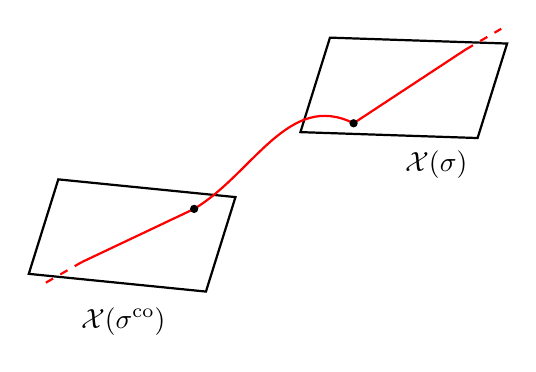
\begin{tikzpicture}[scale=0.75]
\draw[thick] (-4.2,-2.1)--(-1.2,-2.4)--(-0.7,-0.8)--(-3.7,-0.5)--cycle;
\draw[thick] (0.4,0.3)--(3.4,0.2)--(3.9,1.8)--(0.9,1.9)--cycle;
\draw[red,thick] (-3.3,-1.9)--(-1.4,-1.0);
\draw[dashed,red,thick] (-3.3,-1.9)--(-4.0,-2.3);
\draw[red,thick] (1.3,0.45)--(3.2,1.7);
\draw[dashed,red,thick] (3.2,1.7)--(3.8,2.05);
\draw[red,thick] (-1.4,-1.0) .. controls (-0.4,-0.4) and (0.2,1.0) .. (1.3,0.45);
\fill (-1.4,-1.0) circle (2pt);
\fill (1.3,0.45) circle (2pt);
\node at (-2.6,-2.9) {$\XX(\sigma^{\mathrm{co}})$};
\node at (2.7,-0.25) {$\XX(\sigma)$};
\end{tikzpicture}\\[3pt]
{\small $\XX(\sigma)\cong\XX(\sigma^{\mathrm{co}})$，沿其分裂轨迹（split loci）粘连，即 $t\leftrightarrow t^{-1}$。}
\end{center}

令 $X$ 记 $k$ 上一条带寻常二重点的 $\mathbb P^1$ 链，长度为 $(p-1)/2$。我们在 $X$ 的每个不可约分支上选取坐标 $T$，使得每个奇点在一个相交分支上对应 $0$、在另一分支上对应 $\infty$。我们称点 $0$ 与 $\infty$ 为\emph{标记点}（marked points）。

用伴权对 $\sigma,\sigma^{\mathrm{co}}$ 标号 $X$ 的各分支，并把相应的 $\mathbb P^1$ 记作 $X(\sigma|\sigma^{\mathrm{co}})$。各分支的次序由下述要求给出：若 $0<b<p-1$，则分支 $X(\sigma_{a,b}|\sigma_{a+b+1,p-3-b})$ 与分支 $X(\sigma_{a+b,p-1-b}|\sigma_{a+1,b-2})$ 相交。容易验证这样的标号恰有两种（而选取一种标号等同于选取链的一个端点）。

\begin{center}
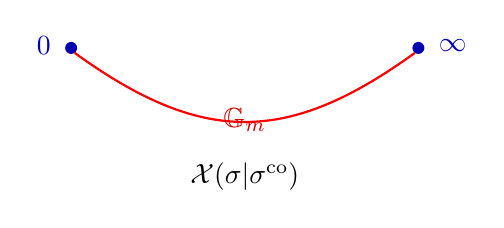
\begin{tikzpicture}[scale=0.9]
\draw[red,thick] (-2.4,0.4) .. controls (-0.6,-0.9) and (0.6,-0.9) .. (2.4,0.4);
\fill[blue!70!black] (-2.45,0.47) circle (2.4pt);
\fill[blue!70!black] (2.45,0.47) circle (2.4pt);
\node[blue!70!black,anchor=east] at (-2.6,0.5) {$0$};
\node[blue!70!black,anchor=west] at (2.6,0.5) {$\infty$};
\node[red!80!black] at (0,-0.55) {$\mathbb G_m$};
\node at (0,-1.35) {$\XX(\sigma|\sigma^{\mathrm{co}})$};
\end{tikzpicture}
\end{center}

这一构造的要点在于：利用我们对叠 $\XX(\sigma)$ 的显式描述，可以定义态射 $\pi:\XX_{\mathrm{red}}\to X$。我们仍满足于在非常 generic 的伴权对 $\sigma,\sigma^{\mathrm{co}}$ 情形给出描述。如下定义态射 $\pi_\sigma:\XX(\sigma|\sigma^{\mathrm{co}})\to X(\sigma|\sigma^{\mathrm{co}})$。按命题 7.2.11 把 $\XX(\sigma)$ 与 $[(\mathbb A^2\setminus\{0\})/\mathbb G_m]$ 等同，并取该处的坐标 $(t,x)$，把 $(t,x)$ 送到 $t$。再把 $\XX(\sigma^{\mathrm{co}})$ 与 $[(\mathbb A^2\setminus\{0\})/\mathbb G_m]$ 等同，并把 $(t,x)$ 送到 $t^{-1}$。注意按定义有 $\pi_{\sigma^{\mathrm{co}}}(x,t)=\pi_\sigma(x,t)^{-1}$。

对每个 Serre 权的伴权对 $\sigma,\sigma^{\mathrm{co}}$，我们在 $\pi_\sigma:\XX(\sigma|\sigma^{\mathrm{co}})\to X(\sigma|\sigma^{\mathrm{co}})$ 与 $\pi_{\sigma^{\mathrm{co}}}:\XX(\sigma|\sigma^{\mathrm{co}})\to X(\sigma|\sigma^{\mathrm{co}})$ 之中选取一个，使得这两个映射在 $X$ 的相邻分支的交点处一致。（这样的映射选取恰有两种，分别对应 $X$ 各分支的两种标号；两种可能的标号之间相差 $\det^{(p-1)/2}$ 的扭。）

\ysrc{282}
\begin{rem}{7.2.17}\label{rem:a4-7-2-17}
若 $\{\sigma,\sigma^{\mathrm{co}}\}$ 是非常 generic 的，则
\[
\XX(\sigma|\sigma^{\mathrm{co}})
\cong\bigl(\mathbb P^1_t\times[(\Spec k[x,y]/(xy))/(\mathbb G_m)_u]\bigr)
\setminus\bigl(0\times[\{x=0\}/\mathbb G_m]\cup\infty\times[\{y=0\}/\mathbb G_m]\bigr),
\]
其中 $\mathbb G_m$ 经 $u\cdot(x,y)=(u^2x,u^{-2}y)$ 作用。闭子叠 $\XX(\sigma)$ 由方程 $y=0$ 切出（此时 $x,t,u$ 对应命题 7.2.11 给出的 $\XX(\sigma)$ 描述中的同名变量），而 $\XX(\sigma^{\mathrm{co}})$ 由 $x=0$ 切出（此时 $y,t^{-1},u^{-1}$ 对应命题 7.2.11 给出的 $\XX(\sigma^{\mathrm{co}})$ 描述中出现的变量 $x,t,u$）。就这一显式描述而言，映射 $\XX(\sigma|\sigma^{\mathrm{co}})\to X(\sigma|\sigma^{\mathrm{co}})$ 就是到 $\mathbb P^1$ 因子的投影。
\end{rem}

\begin{rem}{7.2.18}\label{rem:a4-7-2-18}
可以验证：若 $\sigma_{a,b}$ 是满足 $b\ne0,p-1$ 的 Serre 权，则有同构
\[
\begin{aligned}
\XX(\sigma_{a,b})\cup\XX(\sigma_{a+b,p-1-b})
&\cong\bigl(\Spec k[t_1,t_2]/(t_1t_2)\times[\mathbb P^1_x/(\mathbb G_m)_u]\bigr)\\
&\qquad\setminus\bigl(\{t_1=0\}\times[0/\mathbb G_m]\cup\{t_2=0\}\times[\infty/\mathbb G_m]\bigr),
\end{aligned}
\]
其中 $\mathbb G_m$ 经 $u\cdot x=u^2x$ 作用在 $\mathbb P^1$ 上。

这里我们通过命题 7.2.11 把轨迹 $t_2=0$（相应地 $t_1=0$）与 $\XX(\sigma_{a,b})$（相应地 $\XX(\sigma_{a+b,p-1-b})$）等同，其中 $t_1$ 对应 $t$、$x$ 对应 $x$（相应地 $t_2$ 对应 $t$、$x$ 对应 $x^{-1}$）。
\end{rem}

\begin{center}
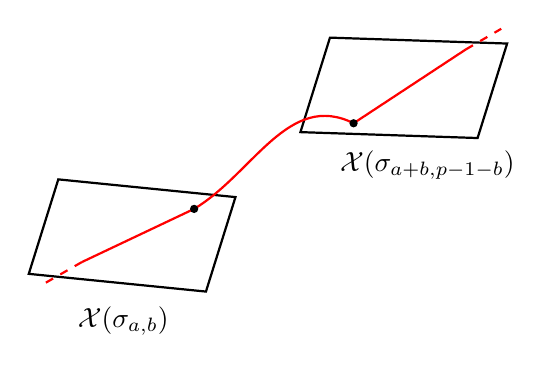
\begin{tikzpicture}[scale=0.75]
\draw[thick] (-4.2,-2.1)--(-1.2,-2.4)--(-0.7,-0.8)--(-3.7,-0.5)--cycle;
\draw[thick] (0.4,0.3)--(3.4,0.2)--(3.9,1.8)--(0.9,1.9)--cycle;
\draw[red,thick] (-3.3,-1.9)--(-1.4,-1.0);
\draw[dashed,red,thick] (-3.3,-1.9)--(-4.0,-2.3);
\draw[red,thick] (1.3,0.45)--(3.2,1.7);
\draw[dashed,red,thick] (3.2,1.7)--(3.8,2.05);
\draw[red,thick] (-1.4,-1.0) .. controls (-0.4,-0.4) and (0.2,1.0) .. (1.3,0.45);
\fill (-1.4,-1.0) circle (2pt);
\fill (1.3,0.45) circle (2pt);
\node at (-2.6,-2.9) {$\XX(\sigma_{a,b})$};
\node at (2.55,-0.25) {$\XX(\sigma_{a+b,p-1-b})$};
\end{tikzpicture}\\[3pt]
{\small $\XX(\sigma_{a,b})\cong\XX(\sigma_{a+b,p-1-b})$，沿其不可约轨迹（irreducible loci）粘连，即 $x\leftrightarrow x^{-1}$。}
\end{center}

由此容易看出，上述对态射 $\pi_\sigma$ 与 $\pi_{\sigma^{\mathrm{co}}}$ 的处方粘成态射 $\XX_{\mathrm{red}}\to X$。

\begin{rem}{7.2.19}\label{rem:a4-7-2-19}
$X$ 与态射 $\pi:\XX_{\mathrm{red}}\to X$ 的定义的动机如下。无论由一般原理，还是由我们对叠 $\XX(\sigma)$ 的显式描述，都容易看出 $X$ 的闭 $\bar\F_p$-点是半单的 $\bar\rho:\Gal_{\Q_p}\to\mathrm{GL}_2(\bar\F_p)$（行列式为 $\bar\varepsilon^{-1}$）。由 $\pi$ 的定义即知它在闭 $\bar\F_p$-点上诱导双射；我们把 $X$ 想成\ysrc{283}$\XX_{\mathrm{red}}$ 的「粗」模空间\footnote{我们给「粗」加上引号，因为态射 $\XX_{\mathrm{red}}\to X$ 并非例如 [Alp14] 技术意义下的粗模空间态射，甚至也不是一个 adequate 模空间态射（例如，因为它在底层拓扑空间上不是闭映射）。不过，它确实满足 [Alp14, Prop. 7.1.1] 的诸条件，特别地，它对从 $\XX_{\mathrm{red}}$ 到局部可分离代数空间的态射是初始的。}。在 $\bar\F_p$-点上，可以把态射 $\pi$ 看作把表示送到其半单化；更显式地说，分支 $X(\sigma|\sigma^{\mathrm{co}})$ 的标记点对应不可约的 $\bar\rho$，而删去标记点后所得的 $\mathbb G_m$ 参数化的是乘积固定、Frobenius 特征值由该 $\mathbb G_m$ 决定的特征之和。
\end{rem}

\begin{rem}{7.2.20}\label{rem:a4-7-2-20}
对 $F$ 的任意选取，都容易构造相应的模空间态射
\begin{equation}\tag{7.2.21}\label{eq:a4-7-2-21}
(\XX_{F,1})_{\mathrm{red}}\lra Y
\end{equation}
使其满足 [Alp14, Prop. 7.1.1] 的诸条件\tn{底本此处排印作「satisfying satisfying the conditions of [Alp14, Prop. 7.1.1] Indeed」，重复了一个 satisfying，且「]」后缺句点；依据为底本原样排印如此，疑为笔误，译文按原意处理。}。事实上，由于 $(\XX_{F,1})_{\mathrm{red}}$ 是形如 $[\Spec A/\mathbb G_m]$ 的全局商叠（其中 $\mathbb G_m$ 平凡地作用），取 $Y=\Spec A$，所得态射 (7.2.21) 甚至是 [Alp13] 意义下的好模空间态射。

进一步，由于 $\XX_{F,1}$ 可以写成 $[\Spf\hat A/\hat{\mathbb G}_m]$ 的形式，其中 $\Spf\hat A$ 是使 $\Spec A$ 加厚（thickens）的 adic 仿射形式概形、带有平凡的 $\hat{\mathbb G}_m$-作用；若再令 $\hat Y:=\Spf\hat A^{\hat{\mathbb G}_m}$，我们便得到态射 $\XX_{F,1}\to\hat Y$，它满足 [Alp14, Prop. 7.1.1] 诸条件的形式代数类比，并把 $\hat Y$ 实现为与 $\XX_{F,1}$ 自身相伴的形式模空间。

回到 $\mathrm{GL}_2(\Q_p)$ 情形。如已提及，我们预期上面构造的态射 $\XX_{\mathrm{red}}\to X$ 也容许一个形式加厚 $\XX\to\hat X$，且满足 [Alp14, Prop. 7.1.1] 诸条件的形式代数类比。另一方面，若 $F\ne\Q_p$ 且 $d\ge2$，甚至当 $F=\Q_p$ 而 $d>2$ 时，我们不预期存在有趣的模空间态射 $\XX_{F,d}\to\hat Y$ 或 $(\XX_{F,d})_{\mathrm{red}}\to Y$。更精确地说，在这些情形我们预期：从 $\XX_{F,d}$ 到局部可分离形式代数空间的任何态射都经过行列式映射 $\XX_{F,d}\to\XX_{F,1}$。
\end{rem}

\subsubsection*{7.2.22.\quad 一些开子叠}

固定非常 generic 的 Serre 权伴权对 $\sigma,\sigma^{\mathrm{co}}$，并用 $U(\sigma|\sigma^{\mathrm{co}})$ 记 $|X(\sigma|\sigma^{\mathrm{co}})|$ 中删去标记点 $0,\infty$ 所得到的开子集。则 $U(\sigma|\sigma^{\mathrm{co}})$ 也是 $|X|$ 中的开集；我们以 $\mathcal U(\sigma|\sigma^{\mathrm{co}})$（有时简记 $\mathcal U$）记 $U(\sigma|\sigma^{\mathrm{co}})$ 的原像，把它看作 $\XX$ 的开子叠。于是 $\mathcal U_{\mathrm{red}}=\mathcal U(\sigma|\sigma^{\mathrm{co}})_{\mathrm{red}}$ 是 $\XX(\sigma|\sigma^{\mathrm{co}})$ 中删去对应不可约 $\bar\rho$ 的轨迹（由两个闭点组成）所得到的（稠密）开子叠；更精确地说，$\mathcal U_{\mathrm{red}}$ 是其两个闭子叠 $\mathcal U\cap\XX(\sigma)$ 与 $\mathcal U\cap\XX(\sigma^{\mathrm{co}})$ 之并。

就注 7.2.17 给出的 $\XX(\sigma|\sigma^{\mathrm{co}})$ 的描述而言，$U(\sigma|\sigma^{\mathrm{co}})_{\mathrm{red}}$ 由
\[
\bigl[(\mathbb G_m\times\Spec k[x,y]/(xy))/\mathbb G_m\bigr]
=[\Spec k[t^{\pm1},x,y]/(xy)/\mathbb G_m]
\]
给出，$\mathbb G_m$-作用为
\[
u\cdot(x,y)=(u^2x,u^{-2}y).
\]

\ysrc{284}
\begin{center}
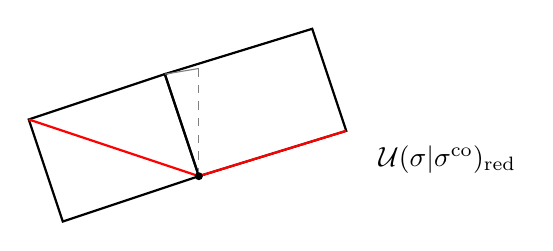
\begin{tikzpicture}[scale=0.72]
\draw[thick] (-3.0,-0.2)--(-0.6,0.6)--(0.0,-1.2)--(-2.4,-2.0)--cycle;
\draw[thick] (-0.6,0.6)--(2.0,1.4)--(2.6,-0.4)--(0.0,-1.2)--cycle;
\draw[red,thick] (-3.0,-0.2)--(0.0,-1.2)--(2.6,-0.4);
\draw[gray,dashed] (0.0,-1.2)--(0.0,0.7);
\draw[gray] (0.0,0.7)--(-0.6,0.6);
\fill (0.0,-1.2) circle (2pt);
\node[anchor=west] at (3.0,-0.9) {$\mathcal U(\sigma|\sigma^{\mathrm{co}})_{\mathrm{red}}$};
\end{tikzpicture}
\end{center}

以形变理论（deformation theory）论证建立在此描述之上，我们可以把 $\mathcal U$ 显式地描述为
\begin{equation}\tag{7.2.23}\label{eq:a4-7-2-23}
\mathcal U(\sigma|\sigma^{\mathrm{co}})
=\bigl[\Spf\mathcal O[s,t^{\pm1},x,y]^{\wedge}/\hat{\mathbb G}_m\bigr],
\end{equation}
其中 hat 指 $(p,s,xy)$-adic 完备化，而 $\hat{\mathbb G}_m$-作用由
\[
u\cdot(s,t,x,y)=(s,t,u^2x,u^{-2}y)
\]
给出。这里 $\mathcal U\cap\XX(\sigma)$ 是轨迹 $\varpi=s=y=0$，$\mathcal U\cap\XX(\sigma^{\mathrm{co}})$ 由 $\varpi=s=x=0$ 给出（与命题 7.2.11 中描述的等同由 $y\mapsto x^{-1}$、$t\mapsto t^{-1}$ 给出）。

\begin{center}
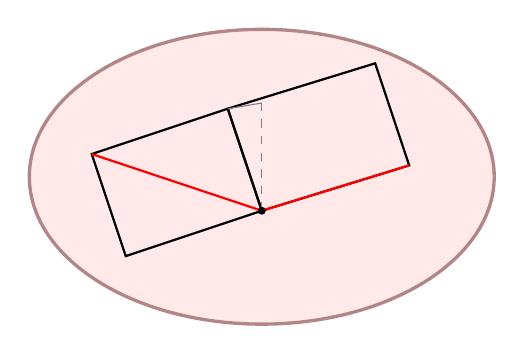
\begin{tikzpicture}[scale=0.72]
\fill[pink!35] (0,-0.6) ellipse (4.1 and 2.6);
\draw[pink!70!black,very thick] (0,-0.6) ellipse (4.1 and 2.6);
\draw[thick] (-3.0,-0.2)--(-0.6,0.6)--(0.0,-1.2)--(-2.4,-2.0)--cycle;
\draw[thick] (-0.6,0.6)--(2.0,1.4)--(2.6,-0.4)--(0.0,-1.2)--cycle;
\draw[red,thick] (-3.0,-0.2)--(0.0,-1.2)--(2.6,-0.4);
\draw[gray,dashed] (0.0,-1.2)--(0.0,0.7);
\draw[gray] (0.0,0.7)--(-0.6,0.6);
\fill (0.0,-1.2) circle (2pt);
\end{tikzpicture}\\[3pt]
{\small $\mathcal U(\sigma|\sigma^{\mathrm{co}})_{\mathrm{red}}$ 位于形式光滑叠 $\mathcal U(\sigma|\sigma^{\mathrm{co}})$ 内部（粉色区域示意后者）。}
\end{center}

\subsubsection*{7.2.24.\quad 更多开子叠}

如注 7.2.18 那样，取满足 $b\ne0,p-1$ 的 Serre 权 $\sigma_{a,b}$。并集 $\XX(\sigma_{a,b})\cup\XX(\sigma_{a+b,p-1-b})$ 含唯一的闭点，其相应的伽罗瓦表示 $\bar\rho$ 不可约。若从该并中删去分裂轨迹（就注 7.2.18 的显式描述而言，即删去轨迹 $x=0$ 与 $x=\infty$），我们得到 $\XX_{\mathrm{red}}$ 的一个含 $\bar\rho$ 的开子集 $\mathcal V_{\mathrm{red}}$，它有显式描述
\[
\mathcal V_{\mathrm{red}}=[\Spec k[t_1,t_2]/(t_1t_2)/\mu_2],
\]
其中 $\mu_2$-作用是平凡的。

\ysrc{285}
若以 $\mathcal V$ 记 $\XX$ 中对应 $\XX_{\mathrm{red}}$ 的开子集 $\mathcal V_{\mathrm{red}}$ 的开子叠，则形变理论论证表明 $\mathcal V$ 有如下描述：
\[
\mathcal V\cong\bigl[\Spf\mathcal O[a,t_1,t_2]^{\wedge}/\mu_2\bigr],
\]
其中 hat 指 $(p,a,t_1t_2)$-adic 完备化，而 $\mu_2$-作用再次是平凡的。

\subsection{$\mathrm{GL}_2(\Q_p)$ 的 Banach 情形 —— II. 证明梗概}

本节我们勾勒期望 7.2.1 的证明。

\subsubsection*{7.3.1.\quad $L_\infty$ 的构造}

我们先定义 $\mathrm{GL}_2(\Q_p)$-表示的 pro-凝聚层 $L_\infty$。本质上，它是 Colmez 的 $\mathrm{GL}_2(\Q_p)$-表示 $D^\natural\boxtimes\mathbb P^1$ 的自然推广。[Col10b] 的一部分论证在我们的设定下几乎原样通过，但另一些则需要更认真的改造。（出现的一些主要困难是：Colmez 的 $D^\natural$ 与 $D^{\mathrm{nr}}$ 与平坦基变换不相容，故凡涉及它们的论证都须重做；此外，当处理一般系数的 $(\varphi,\Gamma)$-模时，格的商不必是字面意义下有限的模，故凡涉及这类有限性陈述的论证也须重做。）

首先注意，按定义 $\XX$ 上存在万有的秩 2 $(\varphi,\Gamma)$-模 $D$。我们发觉在其定义中引入一个扭较为方便，方式如下。若 $A$ 是有限型的 $\mathcal O/\varpi^a$-代数，则态射 $\Spec A\to\XX$ 对应一个带 $A$-系数、行列式为逆分圆特征的秩 2 $(\varphi,\Gamma)$-模，且该 $(\varphi,\Gamma)$-模的构造与 $A$ 中的基变换相容。我们以 $D_A$ 记该 $(\varphi,\Gamma)$-模按分圆特征所作的扭，于是 $D_A$ 的行列式等于分圆特征（而非其逆）。

我们处理全分圆扩张 $\Q_p(\zeta_{p^\infty})/\Q_p$ 的 $(\varphi,\Gamma)$-模，于是 $D_A$ 是环
\[
\mathbf A_A=A((T))
\]
上的秩 2 投射模，配有交换的（$A$-线性的半线性）$\varphi$ 与 $\Gamma$ 作用，其中
\[
\varphi(1+T)=(1+T)^p,
\]
\[
\gamma(1+T)=(1+T)^{\varepsilon(\gamma)}
\]
对任意 $\gamma\in\Gamma$ 成立（其中 $\varepsilon$ 照例是 $p$-进分圆特征）。此外还有 $\varphi$ 的一个左逆 $\psi:D_A\to D_A$；它是 $A$-线性满射、与 $\Gamma$ 交换，并满足
\[
\psi(\varphi(a)m)=a\psi(m),\qquad
\psi(a\varphi(m))=\psi(a)m
\]
对任意 $a\in\mathbf A_A$、$m\in D_A$ 成立。

\ysrc{286}
仿照 Colmez，我们利用 $\varphi,\psi,\Gamma$ 在 $D_A$ 上的作用显式地构造一个 $\mathrm{GL}_2(\Q_p)$-表示。记 $P^+$ 为半群 $\bigl(\begin{smallmatrix}\Z_p\setminus\{0\}&\Z_p\\0&1\end{smallmatrix}\bigr)$，$P$ 为群 $\bigl(\begin{smallmatrix}\Q_p^\times&\Q_p\\0&1\end{smallmatrix}\bigr)$。则 $P^+$ 通过连续映射
\[
\begin{pmatrix}p^ka&b\\0&1\end{pmatrix}z=(1+T)^b\varphi^k\circ\sigma_a(z)
\]
作用在 $D_A$ 上，其中 $a\in\Z_p^\times$、$b\in\Z_p$、$k\in\Z_{\ge0}$，而 $\sigma_a\in\Gamma$ 记满足 $\varepsilon(\sigma_a)=a$ 的元素。

$P^+$ 自然地作用在 $\Z_p$ 上（相应地 $P$ 自然地作用在 $\Q_p$ 上），作用为 $\begin{pmatrix}a&b\\0&1\end{pmatrix}x=ax+b$；如 [Col10c, §3.1] 所述，这一作用可用来在 $\Z_p$ 上定义 $A$-模的 $P^+$-等变层 $\mathcal U\mapsto D_A\boxtimes\mathcal U$。具体做法是：令 $D_A\boxtimes\mathbf Z_p$ 为 $D_A$ 自身；对任意 $i\in\Z_p$ 与 $k\ge0$，$D_A\boxtimes(i+p^k\Z_p)$ 在 $i+p^k\Z_p$ 上的截面定义为 $\begin{pmatrix}p^k&i\\0&1\end{pmatrix}D_A\subseteq D_A$。限制映射 $\operatorname{Res}_{i+p^k\Z_p}:D_A\boxtimes\mathbf Z_p\to D_A\boxtimes(i+p^k\Z_p)$ 由
\[
\begin{pmatrix}1&i\\0&1\end{pmatrix}\circ\varphi^k\circ\psi^k\circ\begin{pmatrix}1&-i\\0&1\end{pmatrix}
\]
给出。于是特别有 $D_A\boxtimes\mathbf Z_p^\times=D_A^{\psi=0}$。

给定 $\Z_p$ 的紧开子集之间的仿射线性映射 $f:U\to V$，有诱导映射 $f_*:M\boxtimes U\to M\boxtimes V$。此定义立刻推广到局部仿射线性的连续映射，再通过取极限推广到可被仿射线性映射适当逼近的函数。特别地，它适用于 $\Z_p^\times$ 上的映射 $z\mapsto1/z$；于是可用该映射把 $D_A\boxtimes\mathbf Z_p$ 沿 $D_A\boxtimes\mathbf Z_p^\times$ 与自身粘成 $\mathbb P^1(\Z_p)(=\mathbb P^1(\Q_p)=\Q_p\cup\{\infty\})$ 上的层。我们以 $D_A\boxtimes\mathbb P^1$ 记该层的整体截面；由函子性，它们带有 $\mathrm{GL}_2(\Q_p)$ 的作用（中心特征平凡）。

由于 $\Q_p$ 是 $\mathbb P^1(\Z_p)$ 的开子集，我们也可以取 $D_A\boxtimes\mathbb P^1$ 在 $\Q_p$ 上的截面，得到一个 $B$-表示，记作 $D_A\boxtimes\Q_p$。展开定义可知，$D_A\boxtimes\Q_p$ 有作为逆极限 $\varprojlim_\psi D_A$ 的显式描述。

$\mathrm{GL}_2(\Q_p)$ 在 $D_A\boxtimes\mathbb P^1$ 上的作用与 $A$ 中的平坦基变换相容，但 $D_A\boxtimes\mathbb P^1$ 并非我们所寻求的 $L_\infty$。这在 [Col10b] 的原设定中已很明显：在那里 $D_A\boxtimes\mathbb P^1$ 实现的不是局部 Langlands 对应，而是该对应由其对偶（带扭）所作的扩张。（关于这一现象在我们设定下的预期推广，见下文 7.3.22 小节。）因此我们（仍仿照 Colmez）把 $L_\infty$ 构造为 $D_A\boxtimes\mathbb P^1$ 的子表示。

为此令 $\mathbf A_A^+=A[[T]]$，它从 $\mathbf A_A$ 继承 $\varphi,\psi,\Gamma$ 的作用。可以证明 $D_A$ 含有极小的 $\psi$-稳定 $\mathbf A_A^+$-格 $D_A^\natural$（「格」意即：它作为 $\mathbf A_A^+$-模有限生成，且在 $\mathbf A_A$ 上张成 $D_A$），其构造与平坦基变换相容。有自然的限制映射
\[
\operatorname{Res}_{\Q_p}:D_A\boxtimes\mathbb P^1\lra D_A\boxtimes\Q_p,
\]
并令
\[
D_A^\natural\boxtimes\mathbb P^1
:=\bigl\{z\in D_A\boxtimes\mathbb P^1,\ \operatorname{Res}_{\Q_p}(z)\in D_A^\natural\boxtimes\Q_p\bigr\},
\]
其中 $D_A^\natural\boxtimes\Q_p:=\varprojlim_\psi D_A^\natural$。

结果是：$D_A^\natural\boxtimes\mathbb P^1$ 是 $D_A\boxtimes\mathbb P^1$ 中的 $\mathrm{GL}_2(\Q_p)$-稳定格，但这完全不显然；事实上，即使在 [Col10b] 的原设定中，$D_A^\natural\boxtimes\mathbb P^1$ 在 $D_A\boxtimes\mathbb P^1$ 中是开的这一点也完全不显然。（这里「格」取 [Dri06] 的意义：$A$ 上 Tate 模中的格是开 $A$-子模 $L$，满足：若 $U\subseteq L$ 是开的，则 $L/U$ 是有限生成 $A$-模。）

证明 $D_A^\natural\boxtimes\mathbb P^1$ 是 $\mathrm{GL}_2(\Q_p)$-稳定格相当复杂；它涉及（通过考虑完备局部环）把情形归结为 $A$ 是 Artinian 的情形，

% 本片止于印刷页 286 页末（§7.3.1），续片自 PDF 300 页起

\ysrc{287}
然后如同 [Col10b] 中那样，最终通过进一步化归到下述显式描述而证得：即 Berger--Breuil [BB10] 所证明的 $\Gal_{\Q_p}$ 的二维晶体表示的 $p$-进局部 Langlands 对应。确立这一点之后，我们便有下述有用的推论。

\begin{cor}{7.3.2 (Dotto--E.--G.)}\label{thm:a4-7-3-2}
设 $p\ge3$。设 $A$ 是某个 $a\ge1$ 的有限型 $\OO/\varpi^a$-代数，且 $D_A$ 是秩 $2$、以 $A$ 为系数、行列式为 $\varepsilon$ 的投射 étale $(\varphi,\Gamma)$-模。则 $D_A^\natural\boxtimes\mathbf P^1$ 是有限 $A[[K]]$-模。
\end{cor}

\begin{proof}
这可由 $D_A^\natural\boxtimes\mathbf P^1$ 在 $\mathrm{GL}_2(\Q_p)$ 作用下的稳定性、$A[[K]]$ 的诺特性，以及下述事实推出：$D_A^\natural$ 作为格，是有限生成 $\mathbf A_A^+$-模。
\end{proof}

进而可以证明，$D_A^\natural\boxtimes\mathbf P^1$ 的构造与 $A$ 上的平坦基变换相容；我们利用这一点构造 $\XX$ 上带有连续 $\mathrm{GL}_2(\Q_p)$-作用的 pro-凝聚层 $L_\infty$。

\subsubsection*{7.3.3.\quad 对 Paškūnas 部分结果的重新解释}
现在回顾 [Paš13] 的一些主要结果，并用我们的函子 $\mathfrak A$ 加以重释。记 $(\mathrm{sm}\,G)^{\mathrm{l.adm}}$ 为 $\mathrm{sm}\,G$ 中由局部容许（locally admissible）表示组成的满子范畴。（按定义，表示 $\pi\in\mathrm{sm}\,G$ 是局部容许的，若每个向量 $v\in\pi$ 都光滑并生成一个容许表示；事实上对 $\mathrm{GL}_2(\Q_p)$，局部容许表示自动局部有限，从而对每个 $v$，由 $v$ 生成的表示都是有限长的。）

与 $\mathrm{sm}\,G$ 不同，范畴 $(\mathrm{sm}\,G)^{\mathrm{l.adm}}$ 容许块（block）分解，现解释如下。按定义，$(\mathrm{sm}\,G)^{\mathrm{l.adm}}$ 的一个块是（同构类的）不可约对象在如下等价关系下的一个等价类：该关系由 $\pi_1\sim\pi_2$（当 $\Ext^1_{\mathrm{sm}\,G}(\pi_1,\pi_2)\neq0$ 或 $\Ext^1_{\mathrm{sm}\,G}(\pi_2,\pi_1)\neq0$ 时）生成。

严格说来，本应写成「不可约容许对象」，但事实上 $\mathrm{sm}\,G$ 的不可约对象全都落在 $(\mathrm{sm}\,G)^{\mathrm{l.adm}}$ 中。确实，特征 $p$ 下 $\mathrm{GL}_2(\Q_p)$ 的、承认中心特征\footnote{后来 Berger 证明 [Ber12]：$\mathrm{GL}_2(\Q_p)$ 在 $\overline{\mathbb F}_p$ 上的不可约光滑表示必定承认中心特征。在我们的特定背景下，我们关心的是 $\mathrm{PGL}_2(\Q_p)$ 的表示，亦即中心特征平凡的 $\mathrm{GL}_2(\Q_p)$ 的表示，因此中心特征这一问题不会出现。}的绝对不可约光滑表示已由 Barthel--Livné 与 Breuil [BL94, Bre03a] 分类，特别地已被证明是容许的。非绝对不可约的情形很容易化归到绝对不可约情形（例如见 [Ber12, Prop. 1.2] 与 [Paš13, §5.13]）。

块 $\mathfrak B$ 如下：
\begin{enumerate}[label=(\arabic*),leftmargin=2.4em,itemsep=0.15em]
\item $\mathfrak B=\{\pi\}$，其中 $\pi$ 是中心特征平凡的超奇异不可约表示；
\item $\mathfrak B=\{\mathrm{Ind}_B^G(\chi\otimes\chi^{-1}),\mathrm{Ind}_B^G(\omega\chi^{-1}\otimes\omega^{-1}\chi)\}$，其中 $\chi:\Q_p^\times\to k^\times$ 是满足 $\chi^2\neq1,\omega^2$ 的某特征\tn{底本此处作 $\chi^2\neq1,\omega^2$；按上下文推断应读作 $\chi^2\notin\{1,\omega^2\}$（上下文推断，无外部依据），译文照录。}；
\item $\mathfrak B=\{\chi,\chi\otimes\mathrm{St}_G,\mathrm{Ind}_B^G(\omega\chi\otimes\omega^{-1}\chi)\}$，其中 $\chi:\Q_p^\times\to k^\times$ 是二次特征；以及
\item 不含绝对不可约对象的块。
\end{enumerate}

\ysrc{288}对我们而言，一个关键观察是：类型 (1)--(3) 的块与 $\XX(k)$ 之间存在双射。（为叙述方便，我们忽略类型 (4) 的块；这类块容易通过允许系数域 $k$ 的有限扩张来处理，它们确实对应于 $\XX$ 在 $k$ 的扩张上的点。）为描述该双射，回忆：对任一 Serre 权 $\sigma$，Hecke 代数
\[
\mathcal H(\sigma):=\End_G(c\text{-Ind}_K^G\sigma)
\]
等于 $k[T]$，其中 $T$ 是某个显式的 Hecke 算子；而绝对不可约表示都是表示
\[
(c\text{-Ind}_K^G\sigma)/(T-\lambda)
\]
（$\lambda\in k$）的子商。此外，除非 $\sigma=\sigma_{a,0}$ 或 $\sigma=\sigma_{a,p-1}$（对某个 $a$）且 $\lambda=\pm1$，这些表示都是（绝对）不可约的；在后一情形有两个 Jordan--Hölder 因子，其形式为 $\chi$、$\chi\otimes\mathrm{St}_G$（对某个 $\chi$）。

块与 $\XX(k)$ 之间的双射依赖于把 Hecke 算子 $T$ 看作 $\XX$ 的分支 $\XX(\sigma|\sigma^{co})$ 中 $\mathbf A^1$ 上的坐标。具体做法如下，仍如上面那样限于一般情形叙述。

\begin{defn}{7.3.4}\label{thm:a4-7-3-4}
设 $\sigma$ 是一般 Serre 权。上文已定义态射 $\XX(\sigma|\sigma^{co})\to\XX(\sigma|\sigma^{co})\subset\XX$，它由 $\pi_\sigma$ 或 $\pi_{\sigma^{co}}$ 之一给出；并固定了 $\XX(\sigma|\sigma^{co})$（同构于 $\mathbf P^1$）上的坐标 $T$。若该态射由 $\pi_\sigma$ 给出，则定义 $f_\sigma:\Spec\mathcal H(\sigma)\to\XX$ 为 $T\mapsto T$；若该态射由 $\pi_{\sigma^{co}}$ 给出，则令 $T\mapsto T^{-1}$。
\end{defn}

于是若 $x$ 是 $\XX$ 的 $k$-点，相应的块由
\[
\mathfrak B_x=\bigcup_{\sigma\ \text{s.t.}\ x\in f_\sigma(\mathbf A^1)}\mathrm{JH}\Bigl(c\text{-Ind}_K^G(\sigma)\otimes_{\mathcal H(\sigma),x}k\Bigr)
\]
给出。更确切地说，$\mathfrak B_x$ 是 $(\mathrm{sm}\,G)_k$ 的一个块，而映射 $x\mapsto\mathfrak B_x$（适当延拓到非一般 Serre 权的情形）是从 $\XX(k)$ 到「含绝对不可约表示的 $\mathrm{sm}\,G$ 的块」之集合的双射。

若 $\mathfrak B$ 是 $(\mathrm{sm}\,G)^{\mathrm{l.adm}}$ 的块，则记 $(\mathrm{sm}\,G)^{\mathrm{l.adm}}_{\mathfrak B}$ 为 $(\mathrm{sm}\,G)^{\mathrm{l.adm}}$ 中由「所有不可约子商都落在给定块 $\mathfrak B$ 中」的表示组成的满子范畴。于是有块分解
\[
(\mathrm{sm}\,G)^{\mathrm{l.adm}}\isom\prod_{\mathfrak B}(\mathrm{sm}\,G)^{\mathrm{l.adm}}_{\mathfrak B}.
\]

在 [Paš13] 中，Paškūnas 建立了范畴 $(\mathrm{sm}\,G)^{\mathrm{l.adm}}_{\mathfrak B}$ 与若干伪形变环上的模范畴之间的范畴等价。我们把 Paškūnas 的结果（及其证明）用作定理 7.2.1 证明的输入；但为此目的，必须把这些结果（某些情形下还要稍加推广）重新表述为关于「映入叠上层范畴的全忠实函子」的陈述。

设 $\bar\theta:\Gal_{\Q_p}\to\mathrm{GL}_2(k)$ 是半单表示（等价地，伪表示），对应于一点 $x\in\XX(k)$。假设（为叙述简便）相应的块 $\mathfrak B_x$ 属于上述情形 (1) 或 (2)；也就是说，假设 $x$ 不是 $\XX(\sigma|\sigma^{co})$ 中满足 $T=\pm1$ 的点，其中 $\{\sigma,\sigma^{co}\}$ 形如 $\{\sigma_{a,0},\sigma_{a+1,p-3}\}$。记
\[
(\mathrm{sm}\,G)^{\mathrm{l.adm}}_{\bar\theta}:=(\mathrm{sm}\,G)^{\mathrm{l.adm}}_{\mathfrak B_x}.
\]

\ysrc{289}
以 $\XX_{\bar\theta}$ 记 Carl Wang-Erickson 的与 $\bar\theta$ 相伴的伽罗瓦表示叠。按定义，$\XX_{\bar\theta}$ 由下述性质刻画：若 $A$ 是 $p$ 在其中幂零的 $\OO$-代数，则 $\XX_{\bar\theta}(A)$ 是连续态射
\[
\rho:\Gal_{\Q_p}\to\mathrm{GL}_2(A)
\]
的群胚，其中 $\det\rho=\varepsilon^{-1}$，且 $\rho$ 模 $\varpi$ 相伴的伪表示等于 $\bar\theta$（此处 $A$ 取离散拓扑，$\Gal_{\Q_p}$ 取自然的投射有限拓扑）。

Wang-Erickson 在 [WE18] 中证明 $\XX_{\bar\theta}$ 是形式代数叠；又由 [EG23, Thm. 6.7.2] 与 [EG24, Thm. 10.2.2]，存在自然的单态射 $\XX_{\bar\theta}\into\XX$，它在底拓扑空间上诱导闭浸入（其像对应于那些半单化同构于 $\bar\theta$ 的表示 $\bar\rho:\Gal_{\Q_p}\to\mathrm{GL}_2(\mathbb F_p)$）。该态射在 $\XX_{\bar\theta}$ 的有限型点处是 versal 的，因此我们自然预期它是形式代数叠 $\XX$ 沿 $\XX_{\mathrm{red}}$ 的闭子叠 $\ZZ_{\bar\theta}$ 的某种完备化；$\ZZ_{\bar\theta}$ 的 $\mathbb F_p$-点正是那些半单化为 $\bar\theta$ 的 $\bar\rho$。

这一预期可用凝聚完备性（coherent completeness）[AHR20, Defn. 2.1] 的语言精确表述如下。以 $\mathcal I_{\bar\theta}$ 记 $\ZZ_{\bar\theta}$ 在 $\XX$ 中的理想层，以 $\XX^{[n]}_{\bar\theta}$ 记 $\XX$ 中由 $\mathcal I^{n+1}_{\bar\theta}$ 截出的闭子叠。则可以证明：对每个 $n$，$\XX^{[n]}_{\bar\theta}$ 是 $\XX_{\bar\theta}$ 的闭子叠；且自然函子（由限制给出）
\[
\Coh(\XX_{\bar\theta})\to\varprojlim_n\Coh(\XX^{[n]}_{\bar\theta})
\]
是范畴等价；也就是说，$\XX_{\bar\theta}$ 上的凝聚层等同于 $\XX$ 中 $\ZZ_{\bar\theta}$ 的各无穷小邻域上的一族相容凝聚层。

给定上述构造，下述定理本质上只是拆解 [Paš13] 主要结果的部分证明。以 $(\mathrm{sm}\,G)^{\mathrm{fg.adm}}_{\bar\theta}$ 记 $(\mathrm{sm}\,G)^{\mathrm{l.adm}}_{\bar\theta}$ 中由有限生成表示组成的满子范畴。

\begin{thm}{7.3.5 (Paškūnas$+\varepsilon$)}\label{thm:a4-7-3-5}
设如上有伪表示 $\bar\theta:\Gal_{\Q_p}\to\mathrm{GL}_2(k)$，其对应的块落在情形 (1) 或 (2)。则函子
\begin{equation}\tag{7.3.6}\label{eq:a4-7-3-6}
(L_\infty)|_{\XX_{\bar\theta}}\otimes_{\OO[[G]]}-
\end{equation}
是从 $(\mathrm{sm}\,G)^{\mathrm{fg.adm}}_{\bar\theta}$ 到 $\XX_{\bar\theta}$ 上凝聚层的范畴的正合全忠实函子。
\end{thm}

\begin{proof}
以 $R^{\mathrm{ps}}_{\bar\theta}$ 记完备诺特局部 $\OO$-代数，它参数化 $\bar\theta$ 在有限型 Artin 局部 $\OO$-代数上的、行列式固定为 $\varepsilon^{-1}$ 的形变；以 $\theta^u$ 记 $\bar\theta$ 在 $R^{\mathrm{ps}}_{\bar\theta}$ 上的泛形变。我们以如下方式定义 Cayley--Hamilton 代数 $\widetilde R_{\bar\theta}$：以 $J$ 记 $R^{\mathrm{ps}}_{\bar\theta}[[\Gal_{\Q_p}]]$ 中由元素 $g^2-\theta^u(g)g+(\varepsilon^{-1})(g)$（$g\in\Gal_{\Q_p}$）生成的双边理想的闭包，然后令
\[
\widetilde R_{\bar\theta}:=R^{\mathrm{ps}}_{\bar\theta}[[\Gal_{\Q_p}]]/J.
\]
\ysrc{290}
如同第 3 节，以 $V$ 记 Colmez 的 Montreal 函子。Paškūnas 在 [Paš13] 中证明环 $\widetilde R_{\bar\theta}$ 作为 $R^{\mathrm{ps}}_{\bar\theta}$-模是秩 $4$ 的自由模；而 [Paš13] 的结果可以解释为：函子 $\pi\mapsto V(\pi)$ 在 $(\mathrm{sm}\,G)^{\mathrm{fg.adm}}_{\bar\theta}$ 与有限长 $\widetilde R_{\bar\theta}$-模范畴之间诱导等价。

存在泛二维 $\Gal_{\Q_p}$-表示 $\mathcal V$ 铺在 $\XX_{\bar\theta}$ 上，可看作带 $\widetilde R_{\bar\theta}$ 作用的秩 $2$ 局部自由 $\OO_{\XX_{\bar\theta}}$-模层。于是利用 [Col10b] 中建立的 $D^\natural\boxtimes\mathbf P^1$ 与 Montreal 函子 $V$ 之间的关系，可以证明函子 (7.3.6) 自然等价于函子
\[
\mathcal V\otimes_{\widetilde R_{\bar\theta}}V(-),
\]
于是由 [Paš13] 中证明的定理容易推出结论。
\end{proof}

类型 (3) 的块（即 $x$ 是 $\XX(\sigma|\sigma^{co})$ 中满足 $T=\pm1$ 的点，其中 $\{\sigma,\sigma^{co}\}$ 形如 $\{\sigma_{a,0},\sigma_{a+1,p-3}\}$ 的情形）更为微妙，因为与其他块不同，我们会看到导出（derived）现象。这一情形最近由 Christian Johansson、James Newton 与 Carl Wang-Erickson [JNWE24] 研究，他们的结果可用于证明下述定理。

\begin{thm}{7.3.7 (Johansson--Newton--Wang-Erickson$+\varepsilon$)}\label{thm:a4-7-3-7}
设如上有伪表示 $\bar\theta:\Gal_{\Q_p}\to\mathrm{GL}_2(k)$，其对应的块 $\mathfrak B_{\bar\theta}=\mathfrak B_x$ 落在情形 (3)。则函子
\begin{equation}\tag{7.3.8}\label{eq:a4-7-3-8}
(L_\infty)|_{\XX_{\bar\theta}}\otimes^{\mathbf L}_{\OO[[G]]}-
\end{equation}
是从 $D(\mathfrak B^{\mathrm{fg}}_{\bar\theta})$ 到 $\XX_{\bar\theta}$ 上凝聚模的有界导出范畴的、幅度为 $[-1,0]$ 的全忠实函子。
\end{thm}

\subsubsection*{7.3.9.\quad 一个有用的消解}
设 $N$ 是通常（上三角）Iwahori 子群 $I$ 的正规化子，$\delta$ 是 $N/ZI$ 的非平凡二次特征。若 $\pi$ 是任一光滑 $G$-表示，则有 $\OO[[G]]$-模复形
\begin{equation}\tag{7.3.10}\label{eq:a4-7-3-10}
0\to c\text{-Ind}_N^G(\delta\pi)\to c\text{-Ind}_K^G(\pi)\to\pi\to0,
\end{equation}
其中第三个箭头是显然的满射 $c\text{-Ind}_K^G\pi\to\pi$。第二个箭头的定义如下。记 $\Pi=\begin{pmatrix}0&1\\p&0\end{pmatrix}$。则态射
\[
v\mapsto\Pi\otimes\Pi^{-1}v-1\otimes v\in\OO[G]\otimes_{\OO[K]}\pi=c\text{-Ind}_K^G\pi
\]
是 $N$-等变态射 $\delta\pi\to c\text{-Ind}_K^G\pi$，它诱导第二个箭头 $c\text{-Ind}_N^G\delta\pi\to c\text{-Ind}_K^G\pi$。容易证明复形 (7.3.10) 无环。

\begin{rem}{7.3.11}\label{thm:a4-7-3-11}
消解 (7.3.10) 对任意 $F/\Q_p$ 的 $\mathrm{PGL}_2(F)$ 都成立，可用于把关于一般 $\pi$ 的某些断言化归到 $\pi=c\text{-Ind}_K^G\sigma$（$\sigma$ 为 Serre 权）的情形。特别地，可用如下方式把连续函子（例如我们假设的函子 $\mathfrak A$）在一般 $\pi$ 上的求值化归到在 $c\text{-Ind}_K^G\sigma$ 上的求值。由于我们假设 $p>2$，$c\text{-Ind}_N^G\delta\pi$ 是 $c\text{-Ind}_I^G\pi=c\text{-Ind}_K^G(c\text{-Ind}_I^K\pi)$ 的直和项，故可化归到研究形如 $c\text{-Ind}_K^GV$ 的表示。
\ysrc{291}由于紧诱导与取滤过余极限相容，我们随后化归到 $V$ 有限生成的情形。由于紧诱导正合，我们进一步化归到 $\pi$ 形如 $c\text{-Ind}_K^G\sigma$（$\sigma$ 为某 Serre 权）的情形，如所断言。
\end{rem}

\subsubsection*{7.3.12.\quad 函子的定义}
现在可以定义我们的函子了。既然已在 $\XX$ 上定义了 $\OO[[G]]$-表示的 pro-凝聚层 $L_\infty$，我们自然想通过
\begin{equation}\tag{7.3.13}\label{eq:a4-7-3-13}
\pi\mapsto L_\infty\otimes^{\mathbf L}_{\OO[[G]]}\pi
\end{equation}
来定义它。然而这一先验地并不显然性质良好，故我们分阶段进行。首先，若 $\pi$ 形如 $c\text{-Ind}_K^GV$ 且 $V$ 有限生成，则注意
\[
L_\infty\otimes^{\mathbf L}_{\OO[[G]]}c\text{-Ind}_K^GV=L_\infty\otimes^{\mathbf L}_{\OO[[K]]}V,
\]
利用推论 7.3.2 可证它是凝聚 $\OO_{\XX}$-模的上有界复形。我们断言它其实是集中于 $0$ 次的层。为看出这点，只需（对上同调次数作降序归纳，并利用上同调群的凝聚性）在每个子叠 $\XX_{\bar\theta}$ 上限制后验证，而那里结论由定理 7.3.5 给出。

过渡到余极限，我们看到对任意 $V$（无论有限生成与否），$L_\infty\otimes^{\mathbf L}_{\OO[[G]]}c\text{-Ind}_K^GV$ 是 $0$ 次拟凝聚层。由注 7.3.11，推出对任意光滑表示 $\pi$，$L_\infty\otimes^{\mathbf L}_{\OO[[G]]}\pi$ 是集中于次数 $[-1,0]$ 的拟凝聚层复形；且若 $\pi$ 有限表现（等价地，有限生成），则该复形具有凝聚上同调层。我们断定 $L_\infty\otimes^{\mathbf L}_{\OO[[G]]}-$ 定义了幅度落在 $[-1,0]$ 中的函子，并把有限表现表示的有界复形送到 $\OO_{\XX}$-模的有界凝聚复形。

\subsubsection*{7.3.14.\quad 局部化与粘合}
若 $\sigma$ 是 Serre 权，我们通过定义 7.3.4 启发式地把 $c\text{-Ind}_K^G\sigma$ 看作「生活」在 $\XX$ 中 $\mathbf A^1=\Spec k[T]=\Spec\mathcal H(\sigma)$ 的某个拷贝之上。这一直观是 [DEG23] 中发展的 $\mathrm{sm}\,G$ 局部化理论的基础；现解释如何使之精确。本节所述结果及其证明大体纯属表示论（偶尔用到块分类，后者在 [Paš13] 中用 $p$-进局部 Langlands 对应证明），当然其动机来自几何图景。

若 $Y$ 是 $X$ 的闭子集\tn{底本对模叠记 $\XX$，对其底拓扑空间则时而记作 $X$（如本句及「$|X|$ 的开子集」）；二者含义不同，译文照录。}，以 $(\mathrm{sm}\,G)_Y$ 记 $\mathrm{sm}\,G$ 中由「所有不可约子商都落在对应于 $Y$ 的闭点的块中」的表示组成的子范畴。若 $U$ 是 $X$ 的开子集，则记
\[
(\mathrm{sm}\,G)_U:=\mathrm{sm}\,G/(\mathrm{sm}\,G)_Y,
\]
其中 $Y:=X\setminus U$。不难验证子范畴 $(\mathrm{sm}\,G)_Y$ 按通常意义是局部化子范畴：即典范商函子 $(j_U)^*:\mathrm{sm}\,G\to(\mathrm{sm}\,G)_U$ 有全忠实右伴随
\[
(j_U)_*:(\mathrm{sm}\,G)_U\to\mathrm{sm}\,G.
\]
在 $U$ 明确时，记 $j_*$ 为 $(j_U)_*$，$j^*$ 为 $(j_U)^*$。

下述结果即 [DEG23, Prop. 3.1.7]，它证实了关于函子 $j_*$、$j^*$ 应有行为的某些基本直观。

\ysrc{292}
\begin{prop}{7.3.15}\label{thm:a4-7-3-15}
设 $Y$ 是 $X$ 的闭子集，记 $U:=X\setminus Y$。
\begin{enumerate}[label=(\arabic*),leftmargin=2.4em,itemsep=0.15em]
\item 若 $\sigma$ 是 Serre 权，且对某个 $g\in\mathcal H(\sigma)$ 有 $f_\sigma^{-1}(Y)=V(g)$（$\Spec\mathcal H(\sigma)$ 的闭子集），则自然映射
\[
c\text{-Ind}_K^G\sigma\to(c\text{-Ind}_K^G\sigma)[1/g]
\]
可等同于态射
\[
c\text{-Ind}_K^G\sigma\to j_*j^*c\text{-Ind}_K^G\sigma.
\]
\item 函子 $j_*$ 正合，且与滤过余极限交换。
\end{enumerate}
\end{prop}

若 $\{U_0,\dots,U_n\}$ 是 $X$ 的任一有限开覆盖，则对 $\mathrm{sm}\,G$ 的任一对象 $\pi$，得到函子性的 Čech 消解
\begin{equation}\tag{7.3.16}\label{eq:a4-7-3-16}
0\to\pi\to\prod_i(j_i)_*(j_i)^*\pi\to\cdots\to(j_{0,\dots,n})_*(j_{0,\dots,n})^*\pi\to0,
\end{equation}
其中照例以 $U_{i\dots k}$ 记 $U_i\cap\cdots\cap U_k$，以 $j_{i\dots k}$ 记 $j_{U_{i\dots k}}$，微分由通常公式给出。下述结果即 [DEG23, Prop. 3.2.3]。

\begin{prop}{7.3.17}\label{thm:a4-7-3-17}
对 $\mathrm{sm}\,G$ 的任一对象 $\pi$，消解 (7.3.16) 无环。
\end{prop}

\begin{proof}
利用消解 (7.3.10)，如注 7.3.11 那样化归到 $\pi=c\text{-Ind}_K^G\sigma$（$\sigma$ 为 Serre 权）的情形。此时命题 7.3.15 允许我们化归到标准断言：仿射概形按区分开集的有限开覆盖所对应的 Čech 复形无环。
\end{proof}

由命题 7.3.17 推出，$\mathrm{sm}\,G$ 是 $X$ 上阿贝尔范畴的叠，如定理 7.2.3 所断言。

我们需要一个关于表示范畴的粘合陈述，它对应于层的 Beauville--Laszlo 粘合。记 $(\mathrm{sm}\,G)^{\mathrm{fg}}$ 为 $\mathrm{sm}\,G$ 中由有限生成对象组成的满子范畴。类似地，对 $X$ 的任一闭子集 $Y$，记 $(\mathrm{sm}\,G)^{\mathrm{fg}}_Y$ 为 $(\mathrm{sm}\,G)_Y$ 中由有限生成对象组成的满子范畴。可以构造形式 pro-对象范畴 $\mathrm{Pro}((\mathrm{sm}\,G)^{\mathrm{fg}}_Y)$。

\begin{defn}{7.3.18}\label{thm:a4-7-3-18}
若 $\pi$ 是 $(\mathrm{sm}\,G)^{\mathrm{fg}}$ 的对象，$Y$ 是 $X$ 的闭子集，则记 $\hat\pi_Y$ 为 $\mathrm{Pro}((\mathrm{sm}\,G)^{\mathrm{fg}}_Y)$ 中的对象「$\varprojlim_I$」$\pi'$，其中 $\pi'$ 遍历 $\pi$ 的、落在 $(\mathrm{sm}\,G)^{\mathrm{fg}}_Y$ 中的所有商。
\end{defn}

下述结果即 [DEG23, Thm. 3.8.1]。

\begin{thm}{7.3.19}\label{thm:a4-7-3-19}
若 $Y$ 有限，则函子 $\pi\mapsto\hat\pi_Y$ 正合，且由沿 $Y$ 的完备化与 $U$ 上的局部化诱导的典范函子
\[
\begin{aligned}
(\mathrm{sm}\,G)^{\mathrm{fg}}\longrightarrow{}&\mathrm{Pro}\bigl((\mathrm{sm}\,G)^{\mathrm{fg}}_Y\bigr)\\
&\times_{\mathrm{Pro}((\mathrm{sm}\,G)^{\mathrm{fg}}_Y)_U}(\mathrm{sm}\,G)^{\mathrm{fg}}_U
\end{aligned}
\]
是范畴等价。
\end{thm}

\ysrc{293}
\subsubsection*{7.3.20.\quad $\mathfrak A$ 的一般描述}
给定 $|X|$ 的开子集 $U$，有局部化范畴 $(\mathrm{sm}\,G)_U$，以及 $\XX$ 的开子叠 $\mathcal U:=\pi^{-1}(U)$。现在取 $U$ 为有限集 $Y$ 的补集，$Y$ 由对应于类型 (1) 或 (3) 的块的点组成；特别地我们删去了标记点。则 $U$ 在 $X$ 中稠密；如下将解释，实际上可以显式描述 $\mathfrak A$ 在 $(\mathrm{sm}\,G)_U$ 上的限制，并证明它是映入 $D(\mathcal U)$ 的全忠实函子。粗略的想法是循 [Paš13] 对类型 (2) 的块的策略，但「沿非分歧方向代数化」。

开集 $U$ 是它与 $|X|$ 各不可约分支之交的不交并，我们逐个处理这些交。本讨论中只限于描述 $U\cap X(\sigma|\sigma^{co})$ 的情形，其中 $\sigma,\sigma^{co}$ 是一对相伴的、非常一般的 Serre 权。该交在 §7.2.22 中记作 $U(\sigma|\sigma^{co})$；为简化记号，现在重新定义 $U$ 为 $U:=U(\sigma|\sigma^{co})$。$U$ 在 $\XX$ 中的原像为开子叠 $\mathcal U:=\mathcal U(\sigma|\sigma^{co})$。

于是我们的目标是描述 $\mathfrak A$ 与到 $\mathcal U$ 的限制之复合；结果表明它经过 $(\mathrm{sm}\,G)_U$ 分解。我们对该复合的描述将是 Morita 理论的，用 $(\mathrm{sm}\,G)_U$ 的一个投射 pro-生成元来表述；而用我们定义 $\mathfrak A$ 所用的层 $L_\infty$ 来构造这个 pro-生成元，是最简单的办法。事实上，使用 $L_\infty$ 的对偶版本 $L^\vee_\infty$ 更方便，它的构造方式与 $L_\infty$ 本身类似（另见下文 §7.3.22）。

现在写下
\[
\mathcal U\setminus\XX(\sigma^{co})=[(\Spf\OO[s,t^{\pm1},x,y^{\pm1}]^\wedge/\widehat{\mathbb G}_m]=[\Spf A/\mu_2],
\]
其中 $A=\OO[s,t^{\pm1},x]^\wedge$（帽子表示 $(p,s,x)$-进完备化），$\mu_2$ 的作用平凡。\tn{底本此式作「$[(\Spf\OO[s,t^{\pm1},x,y^{\pm1}]^\wedge/\widehat{\mathbb G}_m]$」，左圆括号无配对；译文照录。}可以把 $L^\vee_\infty|_{\mathcal U\setminus\XX(\sigma^{co})}$ 看作带 $\mu_2$ 作用的拓扑 $A[[G]]$-模 $P_\alpha$。经过一些工作并与 [Paš13] 的结果比较，可以证明 $P_\alpha$ 是 $\mathrm{Pro}((\mathrm{sm}\,G)_U)$ 的「pro-投射」对象，意即：若 $\pi\to\pi'$ 是 $(\mathrm{sm}\,G)_U$ 中的满态射，则 $\Hom(P_\alpha,\pi)\to\Hom(P_\alpha,\pi')$ 满射。（由于阿贝尔群满射的投射极限未必满射，这并不能推出 $P_\alpha$ 在 $\mathrm{Pro}((\mathrm{sm}\,G)_U)$ 中投射。）

交换 $\sigma$ 与 $\sigma^{co}$ 的角色，得到另一个 pro-投射对象 $P_\beta$。$P_\alpha$ 与 $P_\beta$ 共同生成 $(\mathrm{sm}\,G)_U$。利用定理 7.3.5 计算它们在闭点处的完备化，可以证明 $\mathfrak A(P_\alpha)$ 与 $\mathfrak A(P_\beta)$ 是 $\mathcal U$ 上某些显式的线丛。事实上，在适当解释记号后，它们就是例 C.4.7 中所考虑的分次模 $B(1)$ 与 $B(-1)$ 对应的线丛；而函子 $\mathfrak A:(\mathrm{sm}\,G)_U\to D(\mathcal U)$ 的全忠实性是命题 C.4.9 的直接推论。

\subsubsection*{7.3.21.\quad 函子的全忠实性}
如 §7.3.20 开头那样，以 $U$ 记有限集 $Y$ 的补集，$Y$ 由对应于类型 (1) 或 (3) 的块的点组成。如同往常忽略类型 (3) 的块的问题（它们需要一些额外论证），$\mathfrak A$ 的全忠实性可由 $\mathfrak A:(\mathrm{sm}\,G)_U\to D(\mathcal U)$ 的全忠实性、连同定理 7.3.19 与定理 7.3.5 推出。

\subsubsection*{7.3.22.\quad 与对偶的相容性}
对任一有限型 $\OO/\varpi^a$-代数 $A$，存在 $\mathrm{GL}_2(\Q_p)$-表示的显然短正合列
\begin{equation}\tag{7.3.23}\label{eq:a4-7-3-23}
0\to D_A^\natural\boxtimes\mathbf P^1\to D_A\boxtimes\mathbf P^1\to(D_A\boxtimes\mathbf P^1)/(D_A^\natural\boxtimes\mathbf P^1)\to0.
\end{equation}

\ysrc{294}
该短正合列在 [Col10b] 中起重要作用；利用 Colmez 的结果（通过化归到 $A$ 为 Artin 代数的情形），可以证明 $D_A^\natural\boxtimes\mathbf P^1$ 与 $(D_A\boxtimes\mathbf P^1)/(D_A^\natural\boxtimes\mathbf P^1)$ 之间存在完美对偶配对（最终来自 Tate 局部对偶的留数配对）。

以 $\mathbf D:D^b_{\mathrm{f.p.}}(\mathrm{sm}\,G)\to D^b_{\mathrm{f.p.}}(\mathrm{sm}\,G)$ 记由
\[
\mathbf D(-)=R\Hom(-,\OO[[G]])[4]
\]
定义的反变函子。利用消解 (7.3.10) 容易验证 $\mathbf D$ 的幅度为 $[0,1]$。我们还以 $\mathbf D_{\XX}$ 记由 Grothendieck--Serre 对偶给出的 $D_{\mathrm{coh}}(\XX)$ 的反等价，即 $R\Hom_{\OO_{\XX}}(-,\omega_{\XX})$，其中 $\omega_{\XX}$ 是 $\XX$ 的对偶层，置于 $0$ 次。

由 $L_\infty$ 的构造，可用 (7.3.23) 构造一个扩张
\[
0\to L_\infty\to?\to\mathbf D_{\XX}L_\infty\to0.
\]
该扩张类属于
\[
\Hom_{\OO[[G]]}\bigl(\mathbf D_{\XX}L_\infty,L_\infty[1]\bigr)=\Ext^1_{\OO[[G]]}\bigl(\mathbf D_{\XX}L_\infty,L_\infty\bigr)[1],
\]
而与该扩张类复合，给出 $D^b_{\mathrm{f.p.}}(\mathrm{sm}\,G)$ 上函子的自然态射
\[
R\Hom_{\OO[[G]]}(-,\mathbf D_{\XX}L_\infty)\to R\Hom_{\OO[[G]]}(-,L_\infty)[1];
\]
我们预期可以证明它是同构，从而得到所预期的与对偶的相容性
\[
\mathfrak A\circ\mathbf D\isom(\mathbf D_{\XX}\circ\mathfrak A)[3].
\]
如注 6.1.35 所述，这意味着各种层
\[
\mathfrak A\Bigl(\bigl(c\text{-Ind}_K^GW_\lambda\otimes\sigma^{\mathrm{crys},\circ}(\tau)\bigr)^\wedge\Bigr)
\]
都是 Cohen--Macaulay 的。由于这一性质可通过在 versal 环上拉回来验证，它也更直接地由函子 $\mathfrak A$ 的构造、它与 §7.3.3 所讨论的 Paškūnas 结果的关系、以及 [Paš15] 的结果推出。

\subsection{$\mathrm{GL}_2(\Q_p)$ 的 Banach 情形——III.\ 例}
现在描述函子 $\mathfrak A$ 的一些显式取值，从其在 Serre 权的紧诱导与（绝对）不可约表示上的值开始，然后转向某些与驯顺潜在 Barsotti--Tate 伽罗瓦表示有关的情形。后一类例子还说明了 §6.2.11 中所假定的 Banach 情形与解析情形之间的相容性。

\subsubsection*{7.4.1.\quad Serre 权的紧诱导}
考虑 Serre 权 $\sigma_{a,b}$。首先假设 $b\neq p-1$，即 $\sigma_{a,b}$ 一般。则 $\mathfrak A(c\text{-Ind}_K^G\sigma_{a,b})$ 是 $\XX(\sigma_{a,b})$ 上的线丛。这可预期，例如通过比较相应的 Taylor--Wiles 拼接模即可看出：由 Fontaine--Laffaille 理论，它们在支撑上是自由模；但究竟得到 $\XX(\sigma_{a,b})$ 上哪个线丛，则不那么显然。为描述它，注意由命题 7.2.11（以及 $\mathbf A^2\setminus\{0\}$ 的 Picard 群平凡），有 $\mathrm{Pic}(\XX(\sigma_{a,b}))=\mathbf Z$，且可验证 $\mathfrak A(c\text{-Ind}_K^G\sigma_{a,b})$ 是对应于 $-1\in\mathbf Z$ 的线丛。（这其实由与对偶的相容性所迫；注 6.1.33 的讨论表明 $\mathfrak A(c\text{-Ind}_K^G\sigma_{a,b})$ 必是 $\XX(\sigma_{a,b})$ 上唯一的自对偶线丛。关于 $\mathrm{GL}_2(\Q_{p^2})$ 的相关计算另见 §7.7。）

若 $b=p-1$，则 $\mathfrak A(c\text{-Ind}_K^G\sigma_{a,p-1})$ 是并
\begin{equation}\tag{7.4.2}\label{eq:a4-7-4-2}
\XX(\sigma_{a,0})\cup\XX(\sigma_{a,p-1})^+\cup\XX(\sigma_{a,p-1})^-
\end{equation}
上的线丛。

\ysrc{295}
我们预期该线丛可如下显式描述：由命题 7.2.13，叠 $\XX(\sigma_{a,p-1})^\pm$ 的 Picard 群也同构于 $\mathbf Z$；我们预期可验证 $\mathfrak A(c\text{-Ind}_K^G\sigma_{a,p-1})$ 在 (7.4.2) 中各不可约分支上的限制都对应于 $-1\in\mathbf Z$。

\subsubsection*{7.4.3.\quad 绝对不可约表示}
§7.4.1 的结果使我们能计算 $\mathfrak A$ 在绝对不可约表示上的值。如 §7.3.3 所讨论，它们是表示
\[
(c\text{-Ind}_K^G\sigma)/(T-\lambda)
\]
（$\lambda\in k$）的子商；且除非 $\sigma=\sigma_{a,0}$ 或 $\sigma=\sigma_{a,p-1}$（$a$ 为某值）且 $\lambda=\pm1$，这些表示事实上绝对不可约。假设不在此情形，则可由 $T-\lambda$ 在线丛 $\mathfrak A(c\text{-Ind}_K^G\sigma)$ 上的单射性推出：$\mathfrak A((c\text{-Ind}_K^G\sigma)/(T-\lambda))$ 是支撑在闭轨迹 $\pi_\sigma^{-1}(\lambda)\cap\XX(\sigma)$ 上的秩 $1$ 层。（当 $\lambda\neq0$ 时，我们将在下文 §7.4.4 中更精确地描述这个秩 $1$ 层。）

不出所料，平凡表示与 Steinberg 表示表现出更复杂的行为，这映照了特征零情形下 $\ell$-进表示的相应图景（见注 C.4.5）。存在 $G$-表示的短正合列
\[
0\to c\text{-Ind}_K^G\sigma_{0,0}\to c\text{-Ind}_K^G\sigma_{0,p-1}\to\mathrm{St}\oplus(\mathrm{nr}_{-1}\circ\det)\otimes\mathrm{St}\to0
\]
与
\[
0\to c\text{-Ind}_K^G\sigma_{0,p-1}\to c\text{-Ind}_K^G\sigma_{0,0}\to\mathbf 1\oplus\mathrm{nr}_{-1}\circ\det\to0,
\]
它们与上述 $\mathfrak A(c\text{-Ind}_K^G\sigma_{a,b})$ 的描述相结合，可用于证明 $\mathfrak A(\mathrm{St})$ 是 $\XX(\mathrm{Sym}^{p-1})^+$ 上的线丛，而 $\mathfrak A(\mathbf 1)$ 是 $\XX(\mathrm{Sym}^{p-1})^+$ 上另一个线丛经过上同调次数 $-1$ 的平移。

\subsubsection*{7.4.4.\quad 类型 (2) 的块}
更详细地考虑类型 (2) 的块的情形。此时 $\mathfrak B=\{\pi_1,\pi_2\}$，其中 $\pi_1=\mathrm{Ind}_B^G(\chi\otimes\chi^{-1})$，$\pi_2=\mathrm{Ind}_B^G(\omega\chi^{-1}\otimes\omega^{-1}\chi)$，$\chi:\Q_p^\times\to k^\times$ 是适当一般的特征。在此背景下有非分裂扩张 $0\to\pi_2\to\kappa\to\pi_1\to0$ 与 $0\to\pi_1\to\kappa'\to\pi_2\to0$（各自在同构意义下唯一），我们将描述各种层 $\mathfrak A(\pi_1)$、$\mathfrak A(\pi_2)$、$\mathfrak A(\kappa)$ 与 $\mathfrak A(\kappa')$。

首先注意，可以写成 $\pi_1=(c\text{-Ind}_K^G\sigma)/(T-\lambda)$ 与 $\pi_2=(c\text{-Ind}_K^G\sigma^{co})/(T-\lambda^{-1})$，其中 $\sigma$ 是某个非常一般的 Serre 权、$\sigma^{co}$ 是它的相伴权，$\lambda$ 适当选取。于是所考虑的所有层，其支撑都包含在 $\pi_\sigma^{-1}(\lambda)$ 中。

轨迹 $\pi_\sigma^{-1}(\lambda)$ 是 $\mathcal U(\sigma|\sigma^{co})_{\mathrm{red}}$ 的闭子叠。沿用 (7.2.23) 的记号，有
\[
\mathcal U(\sigma|\sigma^{co})_{\mathrm{red}}:=[\Spec\bigl(k[t^{\pm1},x,y]/(xy)\bigr)/\mathbb G_m],
\]
其中 $\mathbb G_m$-作用为 $u\cdot(x,y)=(u^2x,u^{-2}y)$。此时映射 $\pi_\sigma:\mathcal U(\sigma|\sigma^{co})_{\mathrm{red}}\to\mathbf A^1$ 就是到 $t$-坐标的投影，故
\[
\pi_\sigma^{-1}(\lambda)=\bigl[(\Spec k[x,y]/(xy))/\mathbb G_m\bigr]
\]
（即 $t=\lambda$ 的轨迹）。

可以给 $k[x,y]/(xy)$ 赋予由 $\mathbb G_m$-作用诱导的分次（于是 $x$ 的次数为 $2$，$y$ 的次数为 $-2$），进而把 $\pi_\sigma^{-1}(\lambda)$ 上的凝聚层描述为分次 $k[x,y]/(xy)$-模。于是对所考虑的层有如下描述：

\ysrc{296}
\[
\begin{aligned}
\mathfrak A(\pi_1)&=\bigl(k[x,y]/(y)\bigr)(-1);\\
\mathfrak A(\pi_2)&=\bigl(k[x,y]/(x)\bigr)(1);\\
\mathfrak A(\kappa)&=\bigl(k[x,y]/(xy)\bigr)(-1);\\
\mathfrak A(\kappa')&=\bigl(k[x,y]/(xy)\bigr)(1).
\end{aligned}
\]
（这里扭照常表示分次的平移。）注意显然的短正合列
\[
0\to\bigl(k[x,y]/(x)\bigr)(1)\xrightarrow{y\cdot}\bigl(k[x,y]/(xy)\bigr)(-1)\to\bigl(k[x,y]/(y)\bigr)(-1)\to0
\]
与
\[
0\to\bigl(k[x,y]/(y)\bigr)(-1)\xrightarrow{x\cdot}\bigl(k[x,y]/(xy)\bigr)(1)\to\bigl(k[x,y]/(x)\bigr)(1)\to0;
\]
它们可以解释为对定义 $\kappa$ 与 $\kappa'$ 的短正合列应用 $\mathfrak A$ 所得。

\subsubsection*{7.4.5.\quad 驯顺主级数型}
在本例与下例中，我们处理某些 $p$-进完备化的紧诱导表示，它们与驯顺潜在 Barsotti--Tate 表示有关。我们满足于只勾勒验证全部断言所需的各项计算。

从驯顺主级数情形开始。为此，设 $\{\sigma,\sigma^{co}\}$ 非常一般，$\tau$ 是驯顺主级数型，使得 $\sigma$ 是 $\overline{\sigma}^{\mathrm{crys},\circ}(\tau)$ 的 Jordan--Hölder 因子。注意这蕴涵 $\sigma^{co}$ 不是 $\overline{\sigma}^{\mathrm{crys},\circ}(\tau)$ 的 Jordan--Hölder 因子；确实，若 $\sigma=\sigma_{a,b}$，则 $\overline{\sigma}^{\mathrm{crys},\circ}(\tau)$ 的 Jordan--Hölder 因子是 $\sigma$ 本身，连同 $\sigma_{a+b,p-1-b}$。（确切地说，型 $\overline{\sigma}^{\mathrm{crys},\circ}(\tau)$ 是从 $\mathrm{GL}_2(\mathbb F_p)$ 的主级数表示膨涨而来的，见 §7.7.7。）

于是可以考虑型 $\tau$ 的潜在 Barsotti--Tate 表示之叠 $\XX^{\mathrm{crys},(1,0),\tau}$。可以相当显式地描述 $\XX$ 的这个闭子叠，下面就来这样做。首先要指出，mod $\varpi$ 纤维 $\XX^{\mathrm{crys},(1,0),\tau}$ 等于 $\XX(\sigma_{a,b})\cup\XX(\sigma_{a+b,p-1-b})$。（这是 §6.1.38 所讨论的几何 Breuil--Mézard 猜想对特定型 $\tau$ 的精确形式。）该并集容许注 7.2.18 给出的显式描述，后者把它嵌入为 $\Spec k[t_1,t_2]/(t_1t_2)\times[\mathbf P^1/\mathbb G_m]$ 的开子叠。后一叠可等同于 $p$-进形式代数叠 $(\Spf(\OO[t_1,t_2]/(t_1t_2-p))^\wedge\times[\widehat{\mathbf P}^1/\widehat{\mathbb G}_m]$ 的底约化子叠；而 $\XX^{\mathrm{crys},(1,0),\tau}$ 同构于该形式代数叠中以 $\XX(\sigma_{a,b})\cup\XX(\sigma_{a+b,p-1-b})$ 为底约化子叠的开子叠。

现在转向描述层 $\mathfrak A\bigl((c\text{-Ind}_K^G\sigma^{\mathrm{crys},\circ}(\tau))^\wedge\bigr)$。当然，这依赖于格 $\sigma^{\mathrm{crys},\circ}(\tau)$ 的具体选取。在所有这些格中，有两个特殊的格 $\Lambda_1$ 与 $\Lambda_2$，由「$\Lambda_1$（相应地 $\Lambda_2$）的余基座（cosocle）等于 $\sigma$（相应地 $\sigma_{a+b,p-1-b}$）」这一条件唯一确定（至缩放）。我们可以且确实把这些格正规化，使 $p\Lambda_1\subset\Lambda_2\subset\Lambda_1$。于是（至缩放）任一格 $\Lambda$ 都形如 $\varpi^a\Lambda_1+\Lambda_2$，其中 $0\le a\le e$（$e$ 为系数域 $L$ 的绝对分歧指数）。（$\mathrm{GL}_2$ 的驯顺主级数型中格的这一描述归功于 Breuil [Bre14, §2]，是 [EGS15, Prop. 4.1.4] 的特例。）

若 $\chi:\mathbb F_p^\times\times\mathbb F_p^\times\to\mathbb Z_p^\times\subseteq\OO^\times$ 记 $\sigma$ 的最高权的驯顺提升，我们把它膨涨为（通常上三角）Iwahori 子群 $I$ 的特征，则 $\Lambda_1=\Ind_I^K\chi$；而若 $\chi^s$ 记 $\chi$ 经非平凡 Weyl 群
\ysrc{297}元素 $s$ 的共轭，则 $\Lambda_2=\Ind_I^K\chi^s$。用 $I$ 在 $G$ 中的正规化子里的元素
\[
\begin{pmatrix}0&1\\p&0\end{pmatrix}
\]
作共轭，交换 $\chi$ 与 $\chi^s$，故有同构
\[
c\text{-Ind}_K^G\Lambda_1=c\text{-Ind}_K^G\chi\cong c\text{-Ind}_I^G\chi^s=c\text{-Ind}_K^G\Lambda_2.
\]
把这个同构与由含入 $\Lambda_2\subset\Lambda_1$ 诱导的含入 $c\text{-Ind}_K^G\Lambda_2\into c\text{-Ind}_K^G\Lambda_1$ 复合，得到 $c\text{-Ind}_K^G\Lambda_1$ 的自同态 $U_p$。交换 $\Lambda_1$ 与 $\Lambda_2$ 的角色，得到 $c\text{-Ind}_K^G\Lambda_1$ 的另一个自同态 $U_p'$，满足 $U_pU_p'=p$；并且
\[
\End_G(c\text{-Ind}_K^G\Lambda_1)=\OO[U_p,U_p']/(U_pU_p'-p).
\]
过渡到 $p$-进完备化，得到
\[
\End_G\bigl((c\text{-Ind}_K^G\Lambda_1)^\wedge\bigr)=\OO[U_p,U_p']^\wedge/(U_pU_p'-p).
\]
若 $\Lambda=\varpi^a\Lambda_1+\Lambda_2$，则 $\Lambda$ 在 $\Lambda_1$ 中的含入诱导等同 $c\text{-Ind}_K^G\Lambda=(\varpi^a,U_p)c\text{-Ind}_K^G\Lambda_1$，从而诱导 $p$-进完备化的相应等同 $(c\text{-Ind}_K^G\Lambda)^\wedge=(\varpi^a,U_p)(c\text{-Ind}_K^G\Lambda_1)^\wedge$。这把任一格 $\Lambda$ 的 $\mathfrak A\bigl((c\text{-Ind}_K^G\Lambda)^\wedge\bigr)$ 之计算化归到 $\mathfrak A\bigl((c\text{-Ind}_K^G\Lambda_1)^\wedge\bigr)$ 的计算。

现在取系数域 $L$ 在 $\Q_p$ 上非分歧（确实，特征 $\chi$、从而格 $\Lambda_1$ 都定义在 $\mathbb Z_p$ 上）；在此假设下看到 $\XX^{\mathrm{crys},(1,0),\tau}$ 正则。于是，由于（如 §7.3.22 所述）层 $\mathfrak A\bigl((c\text{-Ind}_K^G\Lambda_i)^\wedge\bigr)$ 是 Cohen--Macaulay 的，Auslander--Buchsbaum 公式表明它是局部自由模，且事实上必须可逆（例如理由如注 6.1.35 所勾勒）。由于 $\Lambda_1^\vee=\Lambda_2$，且 $(c\text{-Ind}_K^G\Lambda_1)^\wedge\cong(c\text{-Ind}_K^G\Lambda_2)^\wedge$，进一步看出该线丛在 $\XX^{\mathrm{crys},(1,0),\tau}$ 上是 Grothendieck--Serre 自对偶的。

现在可以验证 $\mathrm{Pic}([\widehat{\mathbf P}^1/\widehat{\mathbb G}_m])=\mathbf Z\times\mathbf Z$，其中第一个 $\mathbf Z$ 来自 $\mathrm{Pic}(\widehat{\mathbf P}^1)=\mathbf Z$，第二个 $\mathbf Z$ 来自按 $\widehat{\mathbb G}_m$ 的特征作扭。以 $\OO(m)_{\widehat{\mathbf P}^1}(n)$ 记对应于配对 $(m,n)\in\mathbf Z\times\mathbf Z$ 的可逆层。沿复合
\[
\begin{aligned}
f:\XX^{\mathrm{crys},(1,0),\tau}\;&\xrightarrow{\ \text{open}\ }(\Spf(\OO[t_1,t_2]/(t_1t_2-p))^\wedge\times[\widehat{\mathbf P}^1/\widehat{\mathbb G}_m]\\
&\xrightarrow{\ \text{proj.}\ }[\widehat{\mathbf P}^1/\widehat{\mathbb G}_m]
\end{aligned}
\]
拉回，诱导同构
\[
\mathrm{Pic}([\widehat{\mathbf P}^1/\widehat{\mathbb G}_m])\isom\mathrm{Pic}(\XX^{\mathrm{crys},(1,0),\tau}).
\]
此外，$[\widehat{\mathbf P}^1/\widehat{\mathbb G}_m]$ 的对偶层，即 $\OO(-2)_{\widehat{\mathbf P}^1}$，拉回到 $\XX^{\mathrm{crys},(1,0),\tau}$ 的对偶层。于是（由于它自对偶）发现
\[
\mathfrak A\bigl((c\text{-Ind}_K^G\Lambda_1)^\wedge\bigr)\cong f^*\OO(-1)_{\widehat{\mathbf P}^1}.
\]
由于 $\mathfrak A$ 全忠实，还得到同构
\[
\begin{aligned}
\End_G\bigl((c\text{-Ind}_K^G\Lambda_1)^\wedge\bigr)&\isom\Gamma\bigl(\XX^{\mathrm{crys},(1,0),\tau},\OO_{\XX^{\mathrm{crys},(1,0),\tau}}\bigr)\\
&=\OO[t_1,t_2]^\wedge/(t_1t_2-p),
\end{aligned}
\]
它（适当选取 $t_i$ 后）由 $U_p\mapsto t_1$、$U_p'\mapsto t_2$ 给出。对任一格 $\Lambda=\varpi^a\Lambda_1+\Lambda_2$，随后发现
\[
\mathfrak A\bigl((c\text{-Ind}_K^G\Lambda)^\wedge\bigr)=(\varpi^a,t_1)f^*\OO_{\widehat{\mathbf P}^1}(-1).
\]

\ysrc{298}
为了把这些 $\mathfrak A$ 的取值与上面为 Serre 权的紧诱导所算的取值作比较，先注意拉回到特殊纤维诱导同构
\[
\mathrm{Pic}([\widehat{\mathbf P}^1/\widehat{\mathbb G}_m])\isom\mathrm{Pic}([\mathbf P^1/\mathbb G_m]).
\]
然后，若以 $x_0,x_1$ 记 $\mathbf P^1$ 的齐次坐标（于是注 7.2.18 的非齐次坐标 $x$ 等于 $x_1/x_0$），以 $u$ 记 $\mathbb G_m$ 上的坐标，则 $[\mathbf A^1_{x_1/x_0}/(\mathbb G_m)_u]$ 与 $[\mathbf A^1_{x_0/x_1}/(\mathbb G_m)_{u^{-1}}]$ 各自嵌入为 $[\mathbf P^1/\mathbb G_m]$ 的开子叠；限制到这些子叠诱导嵌入
\[
\begin{aligned}
\mathrm{Pic}([\mathbf P^1/\mathbb G_m])&\into\mathrm{Pic}([\mathbf A^1_{x_1/x_0}/(\mathbb G_m)_u])\times\mathrm{Pic}([\mathbf A^1_{x_0/x_1}/(\mathbb G_m)_{u^{-1}}])\\
&=\mathbf Z\times\mathbf Z,
\end{aligned}
\]
由 $(m,n)\mapsto(m+n,m-n)$ 给出。由此计算限制
\[
(f^*\OO(-1)_{\widehat{\mathbf P}^1})|_{\XX(\sigma_{a,b})}=\OO_{\XX(\sigma_{a,b})}(-1)
\]
与
\[
(f^*\OO(-1)_{\widehat{\mathbf P}^1})|_{\XX(\sigma_{a+b,p-1-b})}=\OO_{\XX(\sigma_{a+b,p-1-b})}(-1).
\]
于是，若把 $\mathfrak A$ 作用于短正合列
\[
0\to(c\text{-Ind}_K^G\Lambda_1)^\wedge\xrightarrow{U_p}(c\text{-Ind}_K^G\Lambda_1)^\wedge\to c\text{-Ind}_K^G\sigma_{a,b}\to0,
\]
相应地
\[
0\to(c\text{-Ind}_K^G\Lambda_1)^\wedge\xrightarrow{U_p'}(c\text{-Ind}_K^G\Lambda_1)^\wedge\to c\text{-Ind}_K^G\sigma_{a+b,p-1-b}\to0,
\]
便得到层的短正合列
\[
0\to f^*\OO_{\widehat{\mathbf P}^1}(-1)\xrightarrow{t_1}f^*\OO_{\widehat{\mathbf P}^1}(-1)\to\OO_{\XX(\sigma_{a,b})}(-1)\to0,
\]
相应地
\[
0\to f^*\OO_{\widehat{\mathbf P}^1}(-1)\xrightarrow{t_2}f^*\OO_{\widehat{\mathbf P}^1}(-1)\to\OO_{\XX(\sigma_{a+b,p-1-b})}(-1)\to0.
\]

\subsubsection*{7.4.6.\quad 驯顺尖点型}
对驯顺尖点型的情形，可以作与 §7.4.5 类似的分析。即，存在驯顺尖点型 $\tau$，由「$\sigma^{\mathrm{crys},\circ}(\tau)$ 的 Jordan--Hölder 因子是 $\sigma$ 与 $\sigma^{co}$」这一条件唯一确定。此时潜在 Barsotti--Tate 子叠 $\XX^{\mathrm{crys},(1,0),\tau}$ 是 $\XX(\sigma|\sigma^{co}):=\XX(\sigma)\cup\XX(\sigma^{co})$ 的 $p$-进形式提升。如注 7.2.17 所述，$\XX(\sigma|\sigma^{co})$ 嵌入为 $\mathbf P^1\times[(\Spec k[x,y]/(xy))/\mathbb G_m]$ 的开子叠；而形变论论证表明 $\XX^{\mathrm{crys},(1,0),\tau}$ 同构于 $p$-进形式代数叠 $\widehat{\mathbf P}^1\times[(\Spf(\OO[x,y]/(xy-p))^\wedge/\widehat{\mathbb G}_m]$ 的提升 $\XX(\sigma|\sigma^{co})$ 的开形式代数子叠。\tn{底本此处同样作「$[(\Spf(\OO[x,y]/(xy-p))^\wedge/\widehat{\mathbb G}_m]$」，左圆括号无配对；译文照录。}

同主级数情形一样，$\sigma^{\mathrm{crys}}(\tau)$ 中有两个特殊的格 $\Lambda_1$ 与 $\Lambda_2$，各自至缩放唯一确定，其余基座分别为 $\sigma$ 与 $\sigma^{co}$。固定 $\Lambda_1$ 的选取后，可以缩放 $\Lambda_2$ 使 $p\Lambda_1\subset\Lambda_2\subset\Lambda_1$；任一格都（至缩放）形如 $\Lambda=\varpi^a\Lambda_1+\Lambda_2$，其中 $0\le a\le e$。于是为描述各种层 $\mathfrak A\bigl((c\text{-Ind}_K^G\Lambda)^\wedge\bigr)$，只需描述层 $\mathfrak A\bigl((c\text{-Ind}_K^G\Lambda_1)^\wedge\bigr)$ 与 $\mathfrak A\bigl((c\text{-Ind}_K^G\Lambda_2)^\wedge\bigr)$，以及由含入 $\Lambda_2\subset\Lambda_1$ 诱导的态射
\begin{equation}\tag{7.4.7}\label{eq:a4-7-4-7}
\mathfrak A\bigl((c\text{-Ind}_K^G\Lambda_2)^\wedge\bigr)\to\mathfrak A\bigl((c\text{-Ind}_K^G\Lambda_1)^\wedge\bigr).
\end{equation}

% 本片止于印刷页 298 页末（§7.4.6，公式 (7.4.7)），续片自 PDF 312 页（印刷 299）起

% ch-a4-12.tex —— 第 4 篇（Emerton--Gee--Hellmann）续片，底本 PDF 312--323 = 印刷页 299--310
\ysrc{299}
与主序列情形一样，我们取系数域 $L$ 在 $\Q_p$ 上非分歧（驯顺型总可以定义在非分歧扩张上）；在该假设下我们看到，$\XX^{\mathrm{crys},(1,0),\tau}$ 仍是正则的，从而层 $\mathfrak A\bigl((c\text{-}\mathrm{Ind}_K^G\Lambda_i)^\wedge\bigr)$ 仍是可逆的。此外，由于 $\Lambda_1^\vee=\Lambda_2$，我们发现 $\mathfrak A\bigl((c\text{-}\mathrm{Ind}_K^G\Lambda_1)^\wedge\bigr)$ 与 $\mathfrak A\bigl((c\text{-}\mathrm{Ind}_K^G\Lambda_2)^\wedge\bigr)$ 在 Grothendieck--Serre 对偶下必然互换。

现在拉回给出同构
\[
\mathrm{Pic}\Bigl(\wh{\PP}^{1}\times\bigl[(\Spf(\OO[x,y]/(xy-p))^{\wedge}/\wh{\GG}_m)\bigr]\Bigr)
\isom\mathrm{Pic}\bigl(\XX^{\mathrm{crys},(1,0),\tau}\bigr),
\]
于是 $\XX^{\mathrm{crys},(1,0),\tau}$ 上任一可逆层都必然是 $\mathcal L(n)$ 的形式，其中 $\mathcal L$ 由 $\wh{\PP}^{1}$ 拉回，$n$ 是表明 $\wh{\GG}_m$-作用之权的整数。此外，$\XX^{\mathrm{crys},(1,0),\tau}$ 上的对偶层由 $\wh{\PP}^{1}\times\bigl[(\Spf(\OO[x,y]/(xy-p))^{\wedge}/\wh{\GG}_m)\bigr]$ 上的对偶层 $\OO(-2)_{\wh{\PP}^{1}}$ 拉回得到。

短正合列
\[
0\to(c\text{-}\mathrm{Ind}_K^G\Lambda_2)^\wedge\to(c\text{-}\mathrm{Ind}_K^G\Lambda_1)^\wedge\to c\text{-}\mathrm{Ind}_K^G\sigma\to0
\]
与
\[
0\to(c\text{-}\mathrm{Ind}_K^G\Lambda_1)^\wedge\xrightarrow{\ p\ }(c\text{-}\mathrm{Ind}_K^G\Lambda_2)^\wedge\to c\text{-}\mathrm{Ind}_K^G\sigma^{\mathrm{co}}\to0
\]
在施加 $\mathfrak A$ 之后诱导出相应的层短正合列；而由 $\mathfrak A$ 在 $c\text{-}\mathrm{Ind}_K^G\sigma$ 与 $c\text{-}\mathrm{Ind}_K^G\sigma^{\mathrm{co}}$ 上的已知取值，我们得到
\[
\mathfrak A\bigl((c\text{-}\mathrm{Ind}_K^G\Lambda_1)^\wedge\bigr)\cong\mathcal L(-1),
\]
以及
\[
\mathfrak A\bigl((c\text{-}\mathrm{Ind}_K^G\Lambda_2)^\wedge\bigr)\cong\mathcal L(1),
\]
并且态射 (7.4.7) 由乘以 $y$ 诱导。这一分析并不确定可逆层 $\mathcal L$（因为从 $\PP^{1}$ 拉回的任何 $\mathcal L$，无论限制到 $\XX(\sigma)$ 还是 $\XX(\sigma^{\mathrm{co}})$ 上，都必然平凡）。然而 $\mathcal L(\pm1)$ 的相互对偶性随后表明，$\mathcal L$ 必是 $\OO(-1)_{\wh{\PP}^{1}}$ 的拉回。

\begin{rem}{7.4.8}\label{thm:a4-7-4-8}
尖点情形与主序列情形的一个差别在于：在尖点情形，我们有 $\Gamma\bigl(\XX^{\mathrm{crys},(1,0),\tau},\OO_{\XX^{\mathrm{crys},(1,0),\tau}}\bigr)=\OO$（正如 $\Gamma\bigl(\XX(\sigma|\sigma^{\mathrm{co}}),\OO_{\XX(\sigma|\sigma^{\mathrm{co}})}\bigr)=k$）。经由对函子 $\mathfrak A$ 的考察，这反映了如下事实：紧诱导表示 $\bigl(c\text{-}\mathrm{Ind}_K^G\sigma^{\mathrm{crys},\circ}(\tau)\bigr)^\wedge$ 的自同态环（对晶格 $\sigma^{\mathrm{crys},\circ}(\tau)$ 的任一选取）在此情形下是平凡的。
\end{rem}

\subsubsection*{7.4.9.\quad 与解析情形的相容性示例}
下面暂时允许 $\tau$ 表示驯顺主序列型或驯顺尖点型。此时，正如半稳定情形中 (5.2.14) 所指出的，存在态射
\[
\pi:(\XX^{\mathrm{crys},(1,0),\tau})^{\mathrm{rig}}_\eta\to(\mathrm{Fil}_{(1,0)}\mathrm{WD}_\tau)^{\mathrm{an}},
\]
其目标是二维 Weil--Deligne 表示的（刚性解析）模叠：这些表示的惯性型为 $\tau$、逆分圆行列式固定，并带有一维子空间给出的滤过。

现设 $\tau$ 为主序列型。则
\begin{align*}
(\XX^{\mathrm{crys},(1,0),\tau})^{\mathrm{rig}}_\eta
&\cong\Bigl[\Bigl(\{(t,x)\in(\GG_m)_t\times\PP^{1}_x\mid 1\ge|t|\ge|p|\}\\
&\qquad\setminus\bigl(\{(x,t)\mid 1>|t|,|x|\}\cup\{(x,t)\mid |t|>|p|,|x|>1\}\bigr)\Bigr)\\
&\qquad\Big/\bigl(\wh{\GG}_m\bigr)^{\mathrm{rig}}_\eta\Bigr],
\end{align*}
其中\ysrc{300}$(\wh{\GG}_m)^{\mathrm{rig}}_\eta=\{u\mid |u|=1\}\subset\GG_m$，作用为 $u\cdot(t,x)=(t,u^2x)$；而\footnote{这里我们把乘法群与射影直线（视作刚性解析空间）径直记作 $\GG_m$ 与 $\PP^{1}$。}
\[
(\mathrm{Fil}_{(1,0)}\mathrm{WD}_\tau)^{\mathrm{an}}\cong[(\GG_m)_t\times\PP^{1}_x/(\GG_m)_u],
\]
其作用同样由 $u\cdot(t,x)=(t,u^2x)$ 给出。映射 $\pi$ 此时即是显然的那个。\tn{底本主序列与尖点情形的这两个公式中，集合 $\{(x,t)\mid 1>|t|,|x|\}$ 的 $|x|$ 之后均疑脱漏比较条件；译文照录。}

按此描述，「忘掉滤过」映射 $\mathrm{pr}_{WD}$ 是态射
\[
[(\GG_m)_t\times\PP^{1}_x/(\GG_m)_u]\to[(\GG_m)_t/(\GG_m)_u]
\]
（右端的叠是就 $(\GG_m)_u$ 在 $(\GG_m)_t$ 上的平凡作用构成的）。出现在 (6.2.5) 中的扭 $((-\rho')_\sigma)$ 在此情形下就是如下扭：沿「忘掉 Weil--Deligne 表示」映射
\[
\mathrm{pr}_{Fil}:[(\GG_m)_t\times\PP^{1}_x/(\GG_m)_u]\to\PP^{1}_x/\mathrm{SL}_2
\]
拉回层 $\OO(-1)_{\PP^{1}}$ 所得的扭；该映射由到第二个因子的投影以及 $(\GG_m)_u$ 作为 $\mathrm{SL}_2$ 中对角环面的嵌入共同诱导。\tn{底本此处作「along the the ...」，衍一 the，疑为笔误。}

现在，光滑范畴 Langlands 对应把 $c\text{-}\mathrm{Ind}_K^G\sigma^{\mathrm{crys}}(\tau)$ 对应到 $[(\GG_m)_t/(\GG_m)_u]$ 上带有平凡 $(\GG_m)_u$-等变结构的平凡可逆层。于是 §6.2.11 中预期的相容性 (6.2.13)（同时计入猜想 6.2.4 (1)）预测
\[
\mathfrak A\bigl((c\text{-}\mathrm{Ind}_K^G\sigma^{\mathrm{crys},\circ}(\tau))^\wedge\bigr)^{\mathrm{rig}}_\eta
\cong\mathrm{pr}_{Fil}^{*}\bigl(\OO(-1)_{\PP^{1}}\bigr).
\]
$\PP^{1}_x$ 上的线丛 $\OO(-1)_{\PP^{1}}$ 在投影到 $\PP^{1}_x$ 之下拉回到 $(\GG_m)_t\times\PP^{1}_x$ 的开子集
\begin{align*}
&\{(t,x)\mid 1\ge|t|\ge|p|\}\\
&\qquad\setminus\bigl(\{(x,t)\mid 1>|t|,|x|\}\cup\{(x,t)\mid |t|>|p|,|x|>1\}\bigr)
\end{align*}
上时成为平凡线丛，但它带有非平凡的 $(\GG_m)_u$-作用：事实上 $(\GG_m)_u$ 以权 $-1$ 作用于其上。因此 (6.2.13) 预测同构
\[
\mathfrak A\bigl((c\text{-}\mathrm{Ind}_K^G\sigma^{\mathrm{crys},\circ}(\tau))^\wedge\bigr)^{\mathrm{rig}}_\eta
\cong\OO_{(\XX^{\mathrm{crys},(1,0),\tau})^{\mathrm{rig}}_\eta}(-1),
\]
这与 §7.4.5 的计算相符。

现设 $\tau$ 为尖点型。此时
\begin{align*}
(\XX^{\mathrm{crys},(1,0),\tau})^{\mathrm{rig}}_\eta
&\cong\Bigl[\Bigl(\{(t,x)\in\PP^{1}\times\GG_m\mid 1\ge|x|\ge|p|\}\\
&\qquad\setminus\bigl(\{(t,x)\mid 1>|t|,|x|\}\cup\{(t,x)\mid |t|>1,|x|>|p|\}\bigr)\Bigr)\\
&\qquad\Big/\bigl(\wh{\GG}_m\bigr)^{\mathrm{rig}}_\eta\Bigr],
\end{align*}
其中 $(\wh{\GG}_m)^{\mathrm{rig}}_\eta$ 经 $u\cdot(t,x)=(t,u^2x)$ 作用；而
\[
(\mathrm{Fil}_{(1,0)}\mathrm{WD}_\tau)^{\mathrm{an}}\cong[\PP^{1}_t/\mu_2],
\]
其中 $\mu_2$ 平凡地作用。映射 $\pi$ 此时即是显然的那个，由忘掉 $x$ 给出。

映射 $\mathrm{pr}_{WD}$ 是投影
\[
[\PP^{1}_t/\mu_2]\to[*/\mu_2],
\]
而我们又有映射
\[
\mathrm{pr}_{Fil}:[\PP^{1}_t/\mu_2]\to[\PP^{1}_t/\mathrm{SL}_2]
\]
\ysrc{301}该映射忘掉 Weil--Deligne 表示，并由 $\mu_2$ 到 $\mathrm{SL}_2$ 的中心嵌入诱导。于是预期的相容性 (6.2.13) 预测同构
\[
\mathfrak A\bigl((c\text{-}\mathrm{Ind}_K^G\sigma^{\mathrm{crys},\circ}(\tau))^\wedge\bigr)^{\mathrm{rig}}_\eta
\cong\bigl(\pi^{*}\mathrm{pr}_{Fil}^{*}\OO(-1)_{\PP^{1}}\bigr)(-1)
\]
（外层的扭 $-1$ 表明 $(\wh{\GG}_m)^{\mathrm{rig}}_\eta$ 的等变作用），这与 §7.4.6 的计算相符。（注意：扭 $1$ 与扭 $-1$ 给出 $\XX^{\mathrm{crys},(1,0),\tau}$ 上互不同构的可逆层，但这些线丛拉回到 $(\XX^{\mathrm{crys},(1,0),\tau})^{\mathrm{rig}}_\eta$ 之后变得同构，因为可逆层 $\OO_{(\XX^{\mathrm{crys},(1,0),\tau})^{\mathrm{rig}}_\eta}(2)$ 平凡——它确实以坐标 $x$ 为处处非零的整体截面。）

\subsection{半正交分解}
我们现在阐述 $\IndCoh(\XX)$ 的一个显式半正交分解（其中 $\XX$ 如 §7.2），它使我们能描述函子 $\mathfrak A$ 的本质像。我们还要讨论 $D^\times$（$D$ 是以 $\Q_p$ 为中心的非分裂四元数代数）的表示以及 $\mathrm{GL}_2(\Q_{p^2})$ 的表示所对应的预期函子的类似本质像。

首先注意，我们有态射 $f:\mu_2\times\XX\to\mathcal I_{\XX}$（$\XX$ 的惯性叠），它由 $\zeta\in\mu_2$ 在 $(\varphi,\Gamma)$-模上乘以 $\zeta$ 的作用给出（注意由 $\zeta^2=1$ 知该作用在 $\wedge^2D$ 上平凡）。这个态射还（由构造可见）关于 $\mathcal I_{\XX}$ 上的群胚结构是中心的（$\mathcal I_{\XX}$ 是 $\XX$ 上的群胚）。

态射 $f$ 诱导 $\mu_2$ 在 $\Coh(\XX)$ 上、从而在 $\IndCoh(\XX)$ 上的一个典范作用，如下所述：取形式概形 $U$ 与光滑满射 $U\to\XX$（换言之，$\XX$ 的一张光滑图册），并令 $R:=U\times_{\XX}U$，于是可以写 $\XX=[U/R]$。态射 $f$ 随后在 $U$ 上诱导群胚的态射 $U\times\mu_2\to R$，其中 $\mu_2$ 在 $U$ 上平凡地作用。$\XX$ 上的凝聚层可以看作 $U$ 上带有 $R$-等变结构的凝聚层（这编码了下降到 $\XX$ 的下降数据）；特别地，任何这样的层都带有 $\mu_2$-等变结构，而由 $f$ 的中心性，该结构与 $R$-等变结构交换。因此 $\XX$ 上的凝聚层确实带有典范的 $\mu_2$-等变结构。

令 $\IndCoh(\XX)^{\pm}$ 是 $\IndCoh(\XX)$ 中 $-1\in\mu_2$ 以 $\pm$ 作用的子范畴。我们有时称 $\IndCoh(\XX)^{+}$ 为偶子范畴、$\IndCoh(\XX)^{-}$ 为奇子范畴。

作为走向 $\IndCoh(\XX)$ 的半正交分解的第一步，容易看出我们有正交分解，分成 $\IndCoh(\XX)^{+}$ 与 $\IndCoh(\XX)^{-}$ 两块。由 $L_\infty$ 的构造可得 $L_\infty$ 是奇的，因此 $\mathfrak A$ 的本质像包含在 $\IndCoh(\XX)^{-}$ 中。

\subsubsection*{7.5.1.\quad 动机}
关于半正交分解的一般性讨论，我们请读者参阅附录 A.8。我们的半正交分解由如下可能性所驱动：即注 1.4.6 中所谓的「$p$-进 Fargues--Scholze 猜想」；同时也由 $G$-丛的叠 $\Bun_G$ 在 Fargues--Fontaine 曲线上的结构所驱动，此处 $G=\mathrm{GL}_2(F)$。该叠容许一个分层（stratification），其分层片与特定的等晶体（isocrystal）相对应；而且正如 $\ell$-进情形一样，可以合理地期望：无论考虑 $\Bun_G$ 上何种 $p$-进层的范畴，都会有相应的半正交分解，分成若干块，每一块都可用等晶体的自同构群的表示论来描述。我们\ysrc{302}要提醒读者，我们并不预期本节所考虑的 $\IndCoh(\XX)$ 上的半正交分解会与来自 $\Bun_G$ 的（预期中的）半正交分解精确相符；相反，我们预期二者由一个「上三角幂幺基变换矩阵」相联系，而这个矩阵可能相当复杂。\footnote{Xinwen Zhu 曾向作者们指出，这一情形在某种程度上类似于 [Yun09, §4] 所考虑的层论 Radon 变换。}

\begin{rem}{7.5.2}\label{thm:a4-7-5-2}
把 $p$-进局部 Langlands 表述为范畴等价时，很可能需要对 $\IndCoh(\XX)$ 加上幂零奇异支撑（nilpotent singular support）条件。本节通篇忽略这一点；注意我们大部分时候只涉及叠 $\XX$ 的一般部分，在那里预期该条件是自动成立的。
\end{rem}

\subsubsection*{7.5.3.\quad 来自 $\Bun_G$ 的考量}
正如已经指出的，我们想要展示的 $\IndCoh(\XX)$ 的半正交分解，其结构由一个平行的结构所驱动；后者存在于 $\Bun_G$ 上的可构造层范畴中（其中 $G=\mathrm{GL}_2(F)$ 是我们关心的情形），来自 $\Bun_G$ 上的一个自然分层，我们现在来回忆它。

具体地，依照 [FS24, §I.4] 与 [FS25, §2.6]，叠 $\Bun_{\mathrm{GL}_2}$ 容许如下分层，分成局部闭的分层片。$\Bun_{\mathrm{GL}_2}$ 的连通分支由 $\alpha\in\frac{1}{2}\Z$ 标号，且每个连通分支包含唯一一个开分层片。若 $\alpha\in\Z$，该开分层片同构于 $[*/\mathrm{GL}_2(F)]$；而若 $\alpha\notin\Z$，它同构于 $[*/D^\times]$，其中 $D$ 是以 $F$ 为中心的非分裂四元数代数。（下文我们把群概形的 $p$-进点与对应的层不正式地混为一谈。）其余的分层片由整数对 $(m,n)$ 标号，其中 $m>n$ 且 $m+n=2\alpha$，并等同于商叠 $[*/\mathbf G_{m,n}]$，其中
\[
\mathbf G_{m,n}=\begin{pmatrix}F^\times&\mathrm{BC}(\OO(m-n))\\0&F^\times\end{pmatrix}
\]
是幂幺群菱形（实际上是 Banach--Colmez 空间）$\mathrm{BC}(\OO(m-n))$ 与环面 $F^\times\times F^\times$ 的半直积。（叠 $\Bun_{\mathrm{PGL}_2}$ 可由类似的数据描述：把相差一个由 $\OO(1)$ 给出的扭的等晶体等同起来；例如其连通分支现在由 $\alpha\in\frac{1}{2}\Z/\Z$ 标号。）

在 $\ell$-进情形，$\Bun_{\mathrm{GL}_2}$ 上的层范畴有相应的（无穷）半正交分解，见 [FS24, Thm. I.5.1]；我们预期 $p$-进情形也同样如此。（事实上，我们下文展示的 $\IndCoh(\XX)$ 的半正交分解正是由这一预期所驱动，反过来也印证了它。）在 $\ell$-进情形还可以忽略 Banach--Colmez 空间 $\mathrm{BC}(\OO(m-n))$，但对 $p$-进系数而言这一点先验地并不清楚。如下文所解释的，我们预期它们影响我们的半正交分解当且仅当 $[F:\Q_p]\ge m-n$。（特别地，对 $\mathrm{GL}_2(\Q_p)$，我们发现它们只产生 $\IndCoh(\XX)^{+}$ 的半正交分解中的单个成分，而在 $\IndCoh(\XX)^{-}$ 的分解中完全不起作用——因此特别地也不出现在 $\mathfrak A$ 的本质像的描述中。）

正如已经指出的，在 $F=\Q_p$ 的情形，我们将在下文构造 $\IndCoh(\XX)$ 的一个半正交分解，并特别地把 $\mathfrak A$ 的像描述为如下范畴的左正交补：该范畴由从 $\XX$ 中的\ysrc{303}可约轨迹推出的层所生成。我们进一步给出可约轨迹中的层的半正交分解，具体说是剩余可约轨迹上的层。如上所述，我们预期后一分解最终应与 $\Q_p^\times$ 的表示论相关联。此外，它应当可以用一个「谱 Eisenstein 函子」来描述，其中涉及注 5.3.16 中 Borel $(\varphi,\Gamma)$-模的叠在 Banach 情形下的类似物。

\subsubsection*{7.5.4.\quad 限制到可约轨迹}
我们回到 $F=\Q_p$ 的设定。剩余可约轨迹 $\mathcal U\subset\XX$ 是连通分支 $\mathcal U(\sigma|\sigma^{\mathrm{co}})$ 的并；为叙述方便，一如既往地假定 $\sigma$ 非常一般（very generic）。如 (7.2.23) 所见，我们有 $\mathcal U(\sigma|\sigma^{\mathrm{co}})=[\Spf\,\OO[s,t^{\pm1},x,y]^{\wedge}/\wh{\GG}_m]$，其中上标楔形表示 $(p,s,xy)$-进完备化，且 $x$ 与 $y$ 的权分别为 $2$ 与 $-2$。

令 $A:=\OO[s,t^{\pm1}]$，并令 $B=A[x,y]$，把它看作分次 $A$-代数，其中 $x$ 的权为 $2$、$y$ 的权为 $-2$。令 $I:=(p,s)\subset A$ 与 $J:=(I,xy)\subset B$ 为所指的理想，而 $\mathcal B_J$ 记分次 $B$-模范畴的全子范畴，由那些每个元素都被 $J$ 的某个幂零化的模组成。于是有典范等价
\[
\IndCoh\bigl(\mathcal U(\sigma|\sigma^{\mathrm{co}})\bigr)\isom\IndCoh(\mathcal B_J)
\]
（右端的定义见 (A.6.8) 以及 §C.4.16 的讨论），它在源与靶上都保持 $\pm$-分解（源上关于 $\mu_2$-作用，靶上关于分次的奇偶性）。

由命题 C.4.18 立即可得，每个 $\pm$-成分 $\IndCoh(\mathcal B_J^{\pm})$ 都容许半正交分解，分成半正交的块 $\mathcal D_0^{\pm}$ 与 $\mathcal E_0^{\pm}=(\mathcal D_0^{\pm})^{\perp}$，其中
\[
\mathcal D_0^{+}=\langle B/J\rangle,
\]
\[
\mathcal E_0^{+}=\bigl\langle(A/I)[x](-2),(A/I)[x](-4),\cdots,(A/I)[y](2),(A/I)[y](4),\cdots\bigr\rangle,
\]
\[
\mathcal D_0^{-}=\langle B/J(1),B/J(-1)\rangle,
\]
以及
\[
\mathcal E_0^{-}=\bigl\langle(A/I)[x](-3),(A/I)[x](-5),\cdots,(A/I)[y](3),(A/I)[y](5),\cdots\bigr\rangle.
\]
由 §7.3.20 中我们对函子 $\mathfrak A$ 限制到 $\mathcal U(\sigma|\sigma^{\mathrm{co}})$ 的 Morita 理论构造，我们看到这一限制的像恰好等于 $\mathcal D_0^{-}$。

\subsubsection*{7.5.5.\quad $\mathrm{PGL}_2(\Q_p)$ 情形中 $\mathfrak A$ 的本质像}
我们现在考虑 $\IndCoh(\mathcal U)$ 的半正交分解沿 $j:\mathcal U\to\XX$ 的前推（一如既往地忽略非一般的成分，从而忽略幂零奇异支撑的问题，见附录 A.8.13）。由 (A.8.14)，我们有 $\IndCoh(\XX)^{-}$ 的半正交分解 $\mathcal A_1,\mathcal A_2$，其中 $\mathcal A_2=j_*\mathcal E_0^{-}$，而 $\mathcal A_1=(j^*)^{-1}(\mathcal D_0^{-})$。

我们断言 $\mathcal A_1$ 是 $\mathfrak A$ 的本质像。要看出这一点，注意对 $\mathcal A_1$ 中任何 $x$，我们有态射
\[
x\to j_*j^*x
\]
（来自 $j_*$ 与 $j^*$ 的伴随的单位），其余纤维（cofiber）支撑在 $\mathcal U$ 的补集上。该余纤维因此落在 $\mathfrak A$ 的本质像中，因为这个本质像在超奇异点处包含（奇偶性的）摩天层（它们是超奇异不可约表示的像，见定理 7.3.5）。因此只需证明：\ysrc{304}$\mathfrak A$ 的本质像在 $\mathcal U$ 上的限制正是 $\mathcal D_0^{-}$；而正如我们已经观察到的，这由 §7.3.20 中对该限制的显式描述可得。

\subsubsection*{7.5.6.\quad $D^\times$ 的表示}
为简单起见，我们继续假定 $p\ge5$。

我们先描述猜想性函子 $\mathfrak A_{D^\times}$ 的若干特征：它把中心特征平凡的光滑 $D^\times$-表示取到偶范畴 $\IndCoh(\XX)^{+}$。我们预期这样的函子存在，并且享有与我们关于 $\mathrm{PGL}_2(\Q_p)$ 的函子 $\mathfrak A$ 类似的性质。特别地，我们预期它是连续且全忠实的，并预期它满足与 Taylor--Wiles 拼接的相容性。

利用后一预期，我们可以预测 $\mathfrak A_{D^\times}$ 在一组生成元上的取值。为此我们简要回忆 $D^\times$ 的一些基本表示论。为避免讨论有理性的问题，我们以 $\ol{\F}_p$-系数工作。把 $D$ 的素元记作 $\Pi$，把极大序记作 $\mathcal O_D$，则 $\mathcal O_D/\Pi$ 是 $\F_p$ 的二次扩张，我们把它与 $\F_{p^2}$ 等同。于是 $\mathcal O_D^\times$ 的不可约 $\ol{\F}_p$-表示由 $\F_{p^2}^\times$ 的特征给出。固定嵌入 $\F_{p^2}\into\ol{\F}_p$ 便决定了特征 $\ol{\eta}:\mathcal O_D^\times\to\ol{\F}_p^\times$，而其他每个这样的特征都是某个 $i\in\Z/(p^2-1)\Z$ 对应的 $\ol{\eta}^{i}$ 的形式。这些表示的中心特征平凡，当且仅当 $(p-1)$ 整除 $i$；下文我们总假定如此。此时我们可以把它们延拓为 $\Pi^{2\Z}\mathcal O_D^\times$ 的、中心特征平凡的表示，我们仍记作 $\ol{\eta}^{i}$。

若 $(p+1)\nmid i$，则 $\sigma_i:=\mathrm{Ind}_{\Pi^{2\Z}\mathcal O_D^\times}^{D^\times}\ol{\eta}^{i}$ 是 $D^\times$ 的不可约二维表示（中心特征平凡）；我们有 $\sigma_i\cong\sigma_{-i}$，且当 $i\ne\pm j$ 时 $\sigma_i\not\cong\sigma_j$。若 $i=0$ 或 $i=(p^2-1)/2$，则 $\mathrm{Ind}_{\Pi^{2\Z}\mathcal O_D^\times}^{D^\times}\ol{\eta}^{i}$ 是两个特征 $\sigma_i^{\pm}$ 的直和，满足 $\sigma_i^{\pm}(\Pi)=\pm1$。这些表示给出了「中心特征平凡的光滑 $D^\times$-表示」这一范畴的一组生成元。

我们预期 $\mathfrak A_{D^\times}$ 在这些表示上的取值具有特别简单的形式。T.G. 与 David Geraghty 的模 $p$ Jacquet--Langlands 对应 [GG15] 把 $\ol{\eta}^{i}$ 对应到一对 Serre 权 $\sigma,\sigma^{\mathrm{co}}$ 的伴随对（定义 7.2.14 意义下）。事实上，由注 7.2.15，对 $(\sigma,\sigma^{\mathrm{co}})$ 正是某个尖点驯顺型的 Jordan--Hölder 成分之集；而这个尖点驯顺型对应于（经局部类域论对应于 $\ol{\eta}^{i}\oplus\ol{\eta}^{-i}$ 的 $I_{\Q_p}$ 之表示到特征零的驯顺提升）。

记 $\XX(\sigma_i):=\XX(\sigma)\cup\XX(\sigma^{\mathrm{co}})$。（注意这与定义 7.2.16 中的 $\XX(\sigma|\sigma^{\mathrm{co}})$ 并不总一致，因为我们略去了形如 $\XX(\sigma_{a,p-1})^{\pm}$ 的成分。）于是我们预期（$j=0$ 或 $1$）
\begin{equation}\tag{7.5.7}\label{eq:a4-7-5-7}
\mathfrak A_{D^\times}\bigl(\sigma^{\pm}_{(p^2-1)j/2}\bigr)
=\OO_{\XX(\sigma_{(p-1)j/2,p-1})^{\pm}},
\end{equation}
而当 $(p+1)\nmid i$ 时我们预期
\begin{equation}\tag{7.5.8}\label{eq:a4-7-5-8}
\mathfrak A_{D^\times}(\sigma_i)=\OO_{\XX(\sigma_i)}.
\end{equation}

我们对这一预期的论证如下。由模 $p$ 四元数模形式的重数一（multiplicity one）结果（即相应的拼接模的无挠性结果，见 §7.5.13），以及 $\mathfrak A_{D^\times}$ 与 Taylor--Wiles 拼接的预期相容性，我们预期所有这些层在其支撑（即所指的闭子叠）上都是可逆层。（据我们所知，\ysrc{305}这些重数一结果尚不见于文献，故我们在下文略述其证明。）由于它们也落在 $\IndCoh(\XX)^{+}$ 中，一个自然的猜测是：它们由各自支撑的结构层给出。

\begin{rem}{7.5.9}\label{thm:a4-7-5-9}
看起来合理的是：函子 $\mathfrak A_{D^\times}$ 与猜想 9.3.2 在 Eisenstein 情形下的相容性（对 $\Q$ 上在 $p$ 处分歧的四元数代数）会蕴含这些可逆层确实就是其支撑的结构层，从而为我们的预期提供进一步证据。
\end{rem}

\begin{rem}{7.5.10}\label{thm:a4-7-5-10}
若放弃「表示具有平凡中心特征」这一假设，则上述陈述以显然的方式推广：只要规定 Serre 权 $\sigma_{a,p-2}$ 是它自己的伴随（故此时「伴随对」是单点集）。
\end{rem}

现在我们可以重复 §7.5.5 的分析。我们再次有 $\IndCoh(\XX)^{+}$ 的半正交分解 $\mathcal A_1,\mathcal A_2$，其中 $\mathcal A_2=j_*\mathcal E_0^{+}$，而 $\mathcal A_1=(j^*)^{-1}(\mathcal D_0^{+})$。利用预期 (7.5.7) 与 (7.5.8)，我们看到 $\mathfrak A_{D^\times}$ 的本质像包含在 $\mathcal A_1$ 中，且 $\mathcal A_1$ 由该本质像与不可约点处的（偶）摩天层共同生成。

然而，与 $\mathrm{GL}_2(\Q_p)$ 的情形相反，$\mathfrak A_{D^\times}$ 的本质像并不包含这些摩天层！相反，我们预期这些摩天层由 $\Bun_{\mathrm{PGL}_2}$ 的第一个非开分层片——即由 $\mathrm{BC}(\OO(1))$ 的表示论——所解释。因此我们是在暗示 $\mathrm{BC}(\OO(1))$ 的行为与 $\mathrm{BC}(\OO(n))$（$n>1$）不同；对此我们指出一些理由：$\mathrm{BC}(\OO(n))$ 当 $n=1$ 时可由完满空间表示，而当 $n>1$ 时不能。\tn{底本此处作「these skyscraper accounts are accounted for by…」，其中 accounts 疑为 sheaves 之误；译文按上下文译作「摩天层」。}

\subsubsection*{7.5.11.\quad $\mathrm{GL}_2(\Q_{p^2})$ 的情形}
对 $\mathrm{GL}_2(\Q_{p^f})$ 的情形可以作类似分析。我们可以用与上述关于 $D^\times$ 的预测类似的方式，给出假想函子 $\mathfrak A$ 的本质像的生成元；并且我们可以描述相应叠 $\XX_{\Q_{p^f},2}$ 的不可约成分（对一般的 Serre 权，我们将在 §7.6 做这件事）。人们也可以通过类似于上述的分析，在可约轨迹上构造半正交分解。

$\mathrm{GL}_2(\Q_{p^2})$ 的情形与上述 $D^\times$ 的情形非常相似。我们再次发现（假想的）$\mathfrak A$ 的本质像包含在相应层范畴的偶部分中，并且包含在某个显式层范畴的左正交补中，该显式层范畴由从可约轨迹推出的层生成。我们再次发现不可约点处的摩天层包含在这个左正交补中，但似乎不在 $\mathfrak A$ 的本质像中。

我们再次预期这些摩天层由 Banach--Colmez 空间的表示论所解释，此情形下即 $\mathrm{BC}(\OO(2))$；同样，这个 Banach--Colmez 空间可由完满空间表示。（对一般的 $F$，$\mathrm{BC}(\OO(n))$ 可由完满空间表示当且仅当 $0<n\le[F:\Q_p]$，见 [FS24, Prop. II.2.5(iv)]。）

\begin{rem}{7.5.12}\label{thm:a4-7-5-12}
不可约点处的摩天层不落在 $\mathfrak A$ 的本质像中，这与 $\mathrm{GL}_2(\Q_{p^2})$ 的超奇异表示不能有限呈现有关；见下文 §7.7.59。我们不知道这种有限呈现性的失效是否有纯粹表示论上的解释，即用 $\mathrm{BC}(\OO(2))$ 来解释。\tn{底本此处引「§7.7.59」，与该节段落编号的体例不合，疑为笔误；译文照录。}
\end{rem}

\ysrc{306}
\subsubsection*{7.5.13.\quad 重数一}
本节最后，我们略述上面提到的关于 $D^\times$ 的重数一结果的证明。为完整起见，我们放弃「表示具有平凡中心特征」这一假设。设 $D_\Q$ 是 $\Q$ 上的四元数代数，恰在 $p,\infty$ 处分歧；并设 $\ol{r}:\Gal_\Q\to\mathrm{GL}_2(\ol{\F}_p)$ 使得 $\ol{r}|_{\Gal_{\Q_p}}$ 不可约。设 $\frakm$ 是某个适当的、与 $p$ 互素的 Hecke 代数的对应极大理想。（为简单起见，读者可以设想 $\ol{r}$ 在 $p$ 之外非分歧。）对 $\mathcal O_D^\times$ 的每个特征 $\ol{\eta}^{i}$，我们有相应的四元数模形式空间 $M(\ol{\eta}^{i})$（对群 $D_\Q^\times$），以及拼接模 $M_\infty(\ol{\eta}^{i})$——它是拼接模 $M_\infty(\eta^{i})$ 的模 $p$ 约化，其中 $\eta$ 是 $\ol{\eta}$ 到 $\F_{p^2}^\times$ 的 $\OO^\times$-值特征的提升。

这些拼接模已在 [GS11, GG15, Roz15] 等文中研究；由模性提升定理可以证明 $M_\infty(\eta^{i})$ 是某个环 $R_\infty(\eta^{i})$ 上的极大 Cohen--Macaulay 模。环 $R_\infty(\eta^{i})$ 在加框架形变环 $R_{\ol{\rho}}(\eta^{i})$ 上形式光滑，其中 $\ol{\rho}:=\ol{r}|_{\Gal_{\Q_p}}$；后者可描述如下。

首先，若 $(p+1)\mid i$，则扭之后可设 $i=0$，此时 $R_{\ol{\rho}}(\eta^{i})$ 是非晶体半稳定表示（Hodge--Tate 权为 $0,1$）的加框架形变环。其次，若 $(p+1)\nmid i$，则 $R_{\ol{\rho}}(\eta^{i})$ 是潜在晶体表示（Hodge--Tate 权为 $0,1$、惯性型为 $\eta^{i}\oplus\eta^{-i}$）的加框架形变环。

有了这一描述，容易验证拼接模的支撑与 (7.5.8)、(7.5.7) 的规定相符。（这是四元数模形式的 Serre 猜想的权部分，最初由 T.G. 与 Savitt 在 [GS11] 中证明；区分 $\sigma_i^{\pm}$ 的加细由 Rozensztajn 在 [Roz15, Lem. 6.1.1] 中证明，方法是考虑「扩张型」（extended types），即跟踪某个 Frobenius 的作用。）

现在，若 $R_{\ol{\rho}}(\eta^{i})$ 是正则的，则 $M_\infty(\eta^{i})$ 自动无挠（这是由 Taylor--Wiles 拼接推出重数一结果的通常论证，独立于 Diamond 与 Fujiwara）。特别地，只要 $R_{\ol{\rho}}(\eta^{i})$ 或者形式光滑，或者在 $\OO[[x,y]]/(xy-p)$ 上形式光滑，此结论就成立，其中 $\OO$ 是 $\Q_p$ 的某个适当非分歧扩大的整数环。形变环 $R_{\ol{\rho}}(\eta^{i})$ 已在许多情形下算出。在 $(p+1)\mid i$ 的情形，它们形式光滑（且可非常显式地描述，因为所有提升都是普通的）；而若 $(p+1)\nmid i$，则由 [Sav05, Thm. 1.4] 与 [EGS15, Thm. 7.2.1] 可知，除 $\ol{\rho}$ 是某个非分歧表示的扭、或 $\ol{\rho}|_{I_p}$ 是 $1\oplus\ol{\varepsilon}$ 的扭这两种情形外，它们都是正则的；下文我们把这些情形称为例外情形。

可以「纯思考」地证明（通过对比 Hodge--Tate 权为 $0,p-1$ 的晶体表示的拼接模）：若 $\ol{\rho}$ 是不同的非分歧特征之直和，则 $R_{\ol{\rho}}(\eta^{i})$ 并不正则。事实上，由 [LHMM24] 的结果，它在 $\OO[[x,y]]/(xy-p^2)$ 上形式光滑（至少当 $p$ 充分大时）。此情形下，似乎不太可能不用某些几何输入就证明 $M_\infty(\eta^{i})$ 的无挠性。其余情形下的形变环也在 [LHMM24] 中算出（对充分大的 $p$）；细节见 [LHMM24, §5.5]。

下述关于这些例外情形中无挠性的论证取自 George Boxer、Frank Calegari 与 T.G. 的未发表工作。（它由 Chengxiang Bao、Andrea Dotto 与 Yulia Kotelnikova 独立发现。）由 Nakayama 引理，只需证明相应的四元数模形式特征空间\ysrc{307}$M(\ol{\eta}^{i})[\frakm]$ 在 $\ol{\F}_p$ 上是一维。

\begin{rem}{7.6.1}\label{thm:a4-7-6-1}
熟悉 $\mathrm{GL}_2(\Q_{p^2})$ 的 $p$-进局部 Langlands 纲领中种种困难与神秘之处、并急于看到我们能对它们提供何种线索的读者，可以直接跳到 §7.7.59 与注 7.8.6。
\end{rem}

\subsection{$\mathrm{GL}_2(\Q_{p^f})$ 的 Banach 情形中的预备}
继 $\mathrm{GL}_2(\Q_p)$ 的情形之后，下一个自然要考虑的情形是 $G:=\mathrm{GL}_2(\Q_{p^f})$（$f>1$）；这里一如既往地 $\Q_{p^f}$ 表示 $\Q_p$ 的非分歧扩张，剩余域为 $\F_q:=\F_{p^f}$，并记 $K:=\mathrm{GL}_2(\Z_{p^f})$、$Z=Z(G)$。例如，此情形下的模 $p$ 局部 Langlands 对应已被相当深入地研究，模 $p$ 局部--整体相容性问题亦然。（我们在行文中会顺带回忆这些研究的部分历史；不熟悉的读者不妨参阅 [Bre10a] 以及 [BHH$^{+}$21] 的引言。）另一方面，模 $p$（更一般地，模 $p^n$）光滑 $G$-表示的范畴之结构仍然相当神秘，超奇异不可约容许表示的分类仍未知，而且至今还没有 $\mathrm{GL}_2(\Q_p)$ 情形中 [Col10b] 与 [Pas13] 所例示的那种「传统」模式的模 $p$ 或 $p$-进 Langlands 对应的精确表述。

我们相信，范畴的视角能为这一情形提供不少洞见，既有助于阐明已知结果，也有助于说明为什么 $p$-进 Langlands 对应的传统表述方式显得如此难以捉摸。在接下来的讨论中，我们通过描述我们\footnote{这些想法中的许多是在 M.E. 与 T.G. 同 Ana Caraiani、Michael Harris、Bao Le Hung、Brandon Levin 与 David Savitt 的合作中发展出来的，属于 NSF 资助 1952556「Collaborative Research: Geometric Structures in the p-adic Langlands Program」的支持范围；我们感谢他们允许我们在此描述这些结果。}关于 $\mathrm{GL}_2(\Q_{p^f})$ 的范畴 Langlands 纲领的若干预备结果与预期，来展开这些要点。为便于记号并明确想法，我们主要聚焦 $f=2$ 的情形，但本节开头先作一些对任何 $f$ 都成立的考量。

\begin{rem}{7.6.2}\label{thm:a4-7-6-2}
$\mathrm{GL}_2(\Q_p)$ 情形与 $\mathrm{GL}_2(\Q_{p^2})$ 情形的相似与差异，可由下例说明。两种情形下，对一般的 Serre 权 $\sigma$，函子 $\mathfrak A$ 都把 $c\text{-}\mathrm{Ind}_{KZ}^G\sigma$ 取到支撑在 $\XX_{\mathrm{red}}$ 的相应成分 $\XX(\sigma)$ 上的显式线丛。在 $\mathrm{GL}_2(\Q_p)$ 的情形，这一对应「不太导出」；特别地，简单计算表明：\ysrc{308}超奇异不可约容许表示 $(c\text{-}\mathrm{Ind}_{KZ}^G\sigma)/T$ 被送到支撑在相应不可约伽罗瓦表示处的（扭）摩天层。

对 $\mathrm{GL}_2(\Q_{p^2})$，同样的计算表明 $(c\text{-}\mathrm{Ind}_{KZ}^G\sigma)/T$ 被送到支撑在 $\XX(\sigma)$ 上对应于 $T=0$ 的闭轨迹处的层。然而这一支撑现在是一维的，而且表示 $(c\text{-}\mathrm{Ind}_{KZ}^G\sigma)/T$ 具有无限长度。事实上，我们知道（见 (7.7.53)）它把完整的紧诱导表示 $c\text{-}\mathrm{Ind}_{KZ}^G\sigma'$（对某些权 $\sigma'\ne\sigma$）作为子表示包含在内；由此容易推出：$\mathrm{GL}_2(\Q_{p^2})$ 的超奇异不可约容许表示不可能被取到真正的层（而非层的复形），这与 $\mathrm{GL}_2(\Q_p)$ 的情形（或 $\ell\ne p$ 的情形）形成鲜明对比。
\end{rem}

\subsubsection*{7.6.3.\quad $\XX_{\mathrm{red}}$ 的一般结构}
一如既往，我们固定系数 $\OO$ 为 $\Q_p$ 的某个有限扩张 $L$ 的整数环，并进一步假定存在 $\Q_{p^f}$ 到 $L$ 的嵌入。（换言之，我们可以把 $L$ 看作 $\Q_{p^f}$ 的扩张。）记 $k$ 为 $\OO$ 的剩余域。我们还固定一个特征 $\zeta:\Q_{p^f}^\times\to\OO^\times$，并记 $\XX$ 为分类「定义在 $p$-进完备 $\OO$-代数上、$\Gal_{\Q_{p^f}}$ 的秩 $2$ 投射 étale $(\varphi,\Gamma)$-模」的 Noetherian 形式代数叠，其行列式固定等于 $\zeta\varepsilon^{-1}$。

\subsubsection*{7.6.4.\quad 成分 $\XX(\sigma)$}
正如 $\mathrm{GL}_2(\Q_p)$ 的情形，底层的约化代数子叠 $\XX_{\mathrm{red}}$ 在 $\Spec k$ 上有限呈现，并且是有限多个不可约成分 $\XX(\sigma)$ 的并，这些成分由中心特征为 $\zeta|_{\OO^\times}$ 的 Serre 权 $\sigma$ 标号；唯一的例外是：当 $\sigma$ 是 Steinberg 权的扭时，出现一对成分 $X(\sigma)^{\pm}$\tn{底本此处写作直立体 $X(\sigma)^{\pm}$，与他处花体的 $\XX(\sigma)$ 不一致；译文照录。}。并且一如既往，对一般的 $\sigma$（形如
\[
\sigma=(\Sym^{a_0}\otimes\det^{b_0})\otimes\cdots\otimes(\Sym^{a_i}\otimes\det^{b_i})^{\mathrm{Fr}^{i}}\otimes\cdots\otimes(\Sym^{a_{f-1}}\otimes\det^{b_{f-1}})^{\mathrm{Fr}^{f-1}}
\]
且所有 $a_i$ 满足 $0\le a_i\le p-3$ 者），$\XX(\sigma)$ 可描述为系数在 $k$-代数中的 Fontaine--Laffaille 模的模叠。

一般地，对 $\F_p$ 上的约化群 $G$，相应的 Fontaine--Laffaille 模空间可描述为商 $(U\backslash G)/T$，其中 $U$ 是 $G$ 中某个固定 Borel 的幂幺根，经左平移作用，而 $T$ 是同一 Borel 的极大环面，经 Frobenius 扭共轭作用。在我们的情形，群 $G$ 是 $\mathrm{SL}_2$ 从 $\F_{p^f}$ 到 $\F_p$ 的纯量限制。由于假定 $k$ 包含 $\F_{p^f}$，我们有
\[
G=G_{/k}=\mathrm{SL}_2^{f},
\]
\[
U=U_{/k}=\left(\begin{pmatrix}1&\mathbf G_a\\0&1\end{pmatrix}\right)^{f},
\]
以及
\[
T=T_{/k}=\mathbf G_m^{f},
\]
Frobenius 循环置换各因子。

现在 $\begin{pmatrix}1&\mathbf G_a\\0&1\end{pmatrix}\backslash\mathrm{SL}_2=\mathbf A^{2}\setminus\{0\}$（经 $\begin{pmatrix}x&*\\*&y\end{pmatrix}\mapsto(x,y)$）。于是我们有
\[
U\backslash G:=\prod_{i=0}^{f-1}(\mathbf A^{2}\setminus\{0\})_{(x_i,y_i)}
\]
\ysrc{309}（下标表示我们对坐标的记法）。环面 $T$ 随后经
\[
(t_0,\dots,t_{f-1})\cdot(x_i,y_i)=(t_{i-1}t_ix_i,t_{i-1}t_i^{-1}y_i)
\]
作用。于是（对一般的 $\sigma$）我们发现 $\XX(\sigma)$ 等于商叠
\[
\XX(\sigma)=\Bigl[\Bigl(\prod_{i=0}^{f-1}(\mathbf A^{2}\setminus\{0\})_{(x_i,y_i)}\Bigr)/\mathbf G_m^{f}\Bigr],
\]
其中环面作用由前述公式给出。

$\XX(\sigma)$ 上的坐标 $(x_i,y_i)$ 显然并不完全典范，但也并非完全没有意义；特别地，我们很快会看到，它们的零点轨迹描述 $\XX(\sigma)$ 与其他成分相交的轨迹。乘积
\[
T:=y_0\cdots y_{f-1}
\]
起特殊作用。显然 $T$ 是 $\mathbf G_m^{f}$-不变的，因而在 $\XX(\sigma)$ 上定义一个正则函数。事实上它生成 $\XX(\sigma)$ 上的函数环，我们把它记录为下述引理。

\begin{lem}{7.6.5}\label{thm:a4-7-6-5}
\begin{enumerate}[label=(\arabic*),leftmargin=2.4em,itemsep=0.15em]
\item $\Gamma(\XX(\sigma),\OO_{\XX(\sigma)})=k[T]$。
\item 可区分的开子集 $D(T)$（即 $T$ 的非零轨迹）在 $\XX(\sigma)$ 中恰是 niveau 1 普通轨迹（niveau 1 ordinary locus）。
\end{enumerate}
\end{lem}

具体地，我们看到
\[
D(T)=[\mathbf A^{f}_{(x_0,\dots,x_{f-1})}/(\mathbf G_m)_t]\times(\mathbf G_m)_T,
\]
其中 $t$ 经
\[
t\cdot(x_0,\dots,x_{f-1})=(t^2x_0,\dots,t^2x_{f-1})
\]
作用；因此 $(\mathbf G_m)_t$ 可与 $\mathbf G_m$ 在 $\mathbf G_m^{f}$ 中的对角拷贝等同。存在特征 $\chi:\Gal_{\Q_{p^f}}\to k^\times$（依赖于 $\sigma$），使得 $D(T)$ 的点 $(T,x_0,\dots,x_{f-1})$ 对应于 $\Gal_{\Q_{p^f}}$ 的一个形如
\[
\begin{pmatrix}\mathrm{ur}_T\chi&*\\0&\mathrm{ur}_{T^{-1}}\zeta\varepsilon^{-1}\chi^{-1}\end{pmatrix}
\]
的二维表示 $\ol{\rho}$，其中 $*$ 是 $\Ext^{1}_{\Gal_{\Q_{p^f}}}(\mathrm{ur}_{T^{-1}}\zeta\varepsilon^{-1}\chi^{-1},\mathrm{ur}_T\chi)$ 的一个元素，而该 $\Ext$ 群是 $f$ 维向量空间，坐标为 $x_0,\dots,x_{f-1}$。

零点轨迹 $Z(T):=\XX(\sigma)\setminus D(T)$ 的几何更为复杂；我们在 §7.7 中详细描述 $f=2$ 的情形。

现设 $\sigma$ 非常一般，即每个 $a_i$ 满足 $0<a_i<p-3$。则有 $2f$ 个 Serre 权 $\sigma'$ 使得 $\Ext^{1}_{\mathrm{GL}_2(\F_q)}(\sigma,\sigma')\ne0$，且每个这样的 $\sigma'$ 都是一般的。此时可发现，$\XX(\sigma)$ 与 $\XX(\sigma')$ 恰在 $\XX(\sigma)$ 的一个余维 $1$ 的闭子叠中相交，该闭子叠由 $x_i=0$ 或 $y_i=0$（对某个 $i$）切出。

\ysrc{310}
\subsubsection*{7.6.6.\quad Picard 群}
继续假定 $\sigma$ 一般。由 $\XX(\sigma)$ 作为商叠的描述，容易看出 $\mathrm{Pic}(\XX(\sigma))\cong\Z^{f}$（$\mathbf G_m^{f}$ 的特征标格）。这一同构并不显然典范；但下面我们说明如何使它典范到 $\Z^{f}$ 的坐标置换，附加假设是 $\sigma$ 非常一般。

首先考虑 $\XX(\sigma)$ 的开子叠 $D(T)$。如前所述，它容许描述 $D(T)=(\mathbf A^{f}/\mathbf G_m)\times\mathbf G_m$，由此推出 $\mathrm{Pic}(D(T))=\Z$（$\mathbf G_m$ 的特征标格）。此外，这一等同是典范的，因为出现的 $\mathbf G_m$ 自然地有定向（这对应于如下事实：$D(T)$ 参数化沿固定方向由 $\mathrm{ur}_T\chi$ 扩张 $\mathrm{ur}_{T^{-1}}\zeta\varepsilon^{-1}\chi^{-1}$ 所得的扩张）。

对每个 $i=0,\dots,f-1$，记 $\sigma_i$ 为使 $\XX(\sigma)\cap\XX(\sigma_i)=\XX(\sigma)^{y_i=0}$ 的权；由于 $\sigma$ 非常一般，每个 $\sigma_i$ 也一般。记 $T_i$ 为 $\XX(\sigma_i)$ 上函数 $T$ 的类似物；则
\[
(T_i)|_{\XX(\sigma_i)^{y_i=0}}=\frac{x_{i-1}}{x_i}\prod_{j\ne i-1,i}y_j.
\]
因此
\[
\XX(\sigma)^{y_i=0}\cap D(T_i)=\XX(\sigma)^{y_i=0,\,(x_{i-1}\prod_{j\ne i-1,i}y_j)\ne0}.
\]
现在
\[
D\Bigl(x_{i-1}x_i\prod_{j\ne i-1,i}y_j\Bigr)
=[\mathbf A^{f}_{(x_0,\dots,x_{i-2},y_{i-1},y_i,x_{i+1},\dots,x_{f-1})}/(\mathbf G_m)_t],
\]
其中 $t$ 经
\begin{align*}
&t\cdot(x_0,\dots,x_{i-2},y_{i-1},y_i,x_{i+1},\dots,x_{f-1})\\
&\qquad=(t^2x_0,\dots,t^2x_{i-2},t^2y_{i-1},t^{-2}y_i,t^2x_{i+1},\dots,t^2x_{f-1})
\end{align*}
作用；环面 $(\mathbf G_m)_t$ 可看作 $\mathbf G_m$ 经
\[
t\mapsto(t,\dots,t,t^{-1}\text{ 位于第 }i-1\text{ 个槽位},t,\dots,t)
\]
嵌入 $\mathbf G_m^{f}$ 所得的拷贝。

闭子叠 $\XX(\sigma)^{y_i=0}\cap D(T_i)$ 随后是 $[\mathbf A^{f-1}/\mathbf G_m]$ 被 $y_i=0$ 切出的拷贝。当然，嵌入
\[
\XX(\sigma)^{y_i=0}\cap D(T_i)\into D(T_i)
\]
把 $[\mathbf A^{f-1}/\mathbf G_m]$ 嵌入 $[\mathbf A^{f}/\mathbf G_m]$ 的另一个拷贝。

我们已经观察到 $\mathrm{Pic}(D(T_i))=\mathrm{Pic}([\mathbf A^{f}/\mathbf G_m])=\Z$，且限制映射 $\mathrm{Pic}(D(T_i))\to\mathrm{Pic}([\mathbf A^{f-1}/\mathbf G_m])=\Z$ 是同构。因此 $\mathrm{Pic}(\XX(\sigma)^{y_i=0}\cap D(T_i))=\Z$（典范地）。现在考虑这些限制态射的乘积
\begin{equation}\tag{7.6.7}\label{eq:a4-7-6-7}
\begin{aligned}
\Z^{f}\cong\mathrm{Pic}(\XX(\sigma))&\to\mathrm{Pic}(D(T))\times\prod_{i=0}^{f-1}\mathrm{Pic}(\XX(\sigma)^{y_i=0}\cap D(T_i))\\
&=\Z\times\Z^{f}=\Z^{f+1}.
\end{aligned}
\end{equation}
回顾 $D(T)$ 与各个 $\XX(\sigma)^{y_i=0}\cap D(T_i)$ 作为商 $[\mathbf A^{f}/(\mathbf G_m)_t]$ 与 $[\mathbf A^{f-1}/(\mathbf G_m)_t]$ 的描述，以及这些各个拷贝

% 本片止于印刷页 310 页末（§7.6.6）。上句在底本 PDF 324 页（印刷页 311）继续：
% "…of (G_m)_t into (G_m)^f, we find that this map is given by [公式]"，续片自 PDF 324 页起接「的嵌入……」续译。

% ch-a4-13.tex —— 第 4 篇（Emerton--Gee--Hellmann）续片，底本 PDF 324--335 = 印刷页 311--322

\ysrc{311}……$(\GG_m)_t$ 到 $(\GG_m)^f$ 的嵌入，可得该映射由下式给出
\[
(a_0,\dots,a_{f-1})\mapsto\Bigl(\sum_j a_j,\bigl(\sum_{j\neq i-1}a_j-a_{i-1}\bigr)_{i=0}^{f-1}\Bigr)
=\Bigl(\sum_j a_j,\bigl(\sum_{j=0}^{f-1}a_j-2a_{i-1}\bigr)_{i=0}^{f-1}\Bigr).
\]
于是可见 (7.6.7) 是嵌入，并且可以由 $\Z^{f+1}$ 中的坐标还原各个 $a_i$；显式地，（左）逆由下式给出
\[
(b,b_0,\dots,b_i,\dots,b_{f-1})\mapsto\frac12(b-b_1,\dots,b-b_{i+1},\dots,b-b_0).
\]
现在坐标 $(b,b_0,\dots,b_{f-1})$ 是典范的，至多相差对 $b_i$ 的置换（对应于对 $\sigma_i$ 的重新标号）；因此同构 $\mathrm{Pic}(\XX(\sigma))\cong\Z^f$ 是典范的，至多相差对坐标 $a_i$ 的置换。

\subsubsection*{7.6.8.\quad 驯顺型}
若 $\tau$ 是 $\Q_{p^f}$ 的驯顺惯性型（tame inertial type），则相应的 $K$-表示 $\sigma^{\mathrm{crys}}(\tau)$ 通过 $\mathrm{GL}_2(k_F)=\mathrm{GL}_2(\F_{p^f})$ 分解。若 $\sigma^{\mathrm{crys}}(\tau)^\circ$ 是 $\sigma^{\mathrm{crys}}(\tau)$ 中的 $K$-不变格（lattice），则其约化的 Jordan--Hölder 因子的多重集事实上是一个互异 Serre 权（Serre weight）的集合，它不依赖格的具体选取；我们把它记作 $\mathrm{JH}\bigl(\ol{\sigma^{\mathrm{crys}}(\tau)}\bigr)$。若 $\tau$ 进一步充分 generic，则 $\mathrm{JH}\bigl(\ol{\sigma^{\mathrm{crys}}(\tau)}\bigr)$ 恰由 $2^f$ 个权组成。

我们写 $\XX(\tau)=\bigcup_{\sigma\in\mathrm{JH}(\ol{\sigma^{\mathrm{crys}}(\tau)})}\XX(\sigma)$；这是 $\XX_{\mathrm{red}}$ 的闭子叠（closed substack）。

\begin{thm}{7.6.9}\label{thm:a4-7-6-9}
若 $\tau$ 是充分 generic 的驯顺型，则 $\mathrm{Pic}(\XX(\tau))\cong\Z^{2^f}$。
\end{thm}

事实上，限制映射的乘积
\[
\mathrm{Pic}(\XX(\tau))\hookrightarrow\prod_{\sigma\in\mathrm{JH}(\ol{\sigma^{\mathrm{crys}}(\tau)})}\mathrm{Pic}(\XX(\sigma))
\]
是单射，并且可以把 $\mathrm{Pic}(\XX(\tau))$ 的像等同于目标的一个特定子群。

\subsubsection*{7.6.10.\quad 函子的取值}
[EGS15] 的结果表明：若 $\sigma$ 是 generic 的 Serre 权，或 $\sigma^{\mathrm{crys}}(\tau)^\circ$ 是充分 generic 的驯顺型 $\tau$（其行列式等于 $\zeta|_{\OO_F^\times}$）的适当选取的格，则由适当的 Shimura 曲线背景构造出的拼接模 $M_\infty(\sigma)$ 与 $M_\infty\bigl(\sigma^{\mathrm{crys}}(\tau)^\circ\bigr)$ 在其支撑上秩一自由。Serre 猜想的权部分，与可能 Barsotti--Tate 表示的（几何）Breuil--Mézard 猜想，蕴含 $M_\infty(\sigma)$ 的支撑恰是对应通用环上 $\XX(\sigma)$ 的拉回；类似地，$M_\infty\bigl(\sigma^{\mathrm{crys}}(\tau)^\circ\bigr)$ 的支撑是 $\XX(\tau)$ 的拉回。（见 [EG23, Thm. 8.6.2]。）因此我们预期：函子 $\mathfrak A$ 在 $c\text{-}\mathrm{Ind}^G_{KZ}\sigma$ 或 $c\text{-}\mathrm{Ind}^G_{KZ}\sigma^{\mathrm{crys}}(\tau)^\circ$ 上的取值，将分别是 $\XX(\sigma)$ 或 $\XX(\tau)$ 上的线丛。这解释了我们对计算这些叠的 Picard 群的兴趣。

更一般地，若 $V$ 是 $\mathrm{GL}_2(k_F)$ 在 $F$ 上的表示，它重数自由（multiplicity free，即其每个 Jordan--Hölder 因子出现的重数恰为一），且其中心特征（central character）等于 $\ol\zeta$，则 $\mathfrak A$ 在 $c\text{-}\mathrm{Ind}^G_{KZ}V$ 上的取值应当概形论地支撑（scheme-theoretically supported）在 $\bigcup_{\sigma\in\mathrm{JH}(V)}\XX(\sigma)$ 上，特别地支撑在 $\XX_{\mathrm{red}}$ 上。（这来自与 Breuil--Mézard 猜想的预期相容性，以及 $\mathfrak A(c\text{-}\mathrm{Ind}^G_{KZ}V)$ 的预期极大 Cohen--Macaulay 性质。）

\ysrc{312}\begin{thm}{7.6.11（预期定理；Caraiani--E.--G.--Harris--Le Hung--Levin--Savitt）}\label{thm:a4-7-6-11}
存在全忠实函子 $\mathfrak A$，从由诸对象 $c\text{-}\mathrm{Ind}^G_{KZ}V$（其中 $V$ 重数自由，且其所有 Jordan--Hölder 因子都充分 generic）生成的有限表现光滑表示的加法范畴，到 Abel 范畴 $\Coh(\XX_{\mathrm{red}})$。
\end{thm}

本定理中的函子 $\mathfrak A$——我们当然相信它是猜想 6.1.15 的函子 $\mathfrak A$ 对 $\mathrm{GL}_2(\Q_{p^f})$ 的限制——由显式构造产生，其基础是上面给出的各个 Picard 群的描述。特别地，我们有如下预期。

\begin{thm}{7.6.12（预期）}\label{thm:a4-7-6-12}
设 $G=\mathrm{GL}_2(\Q_{p^f})$，且 $\sigma$ 是非常 generic 的 Serre 权；则层 $\mathfrak A(c\text{-}\mathrm{Ind}^G_{KZ}\sigma)$ 是 $\XX(\sigma)$ 上的线丛 $\OO(-1,\dots,-1)$，即对应于元素 $(-1,\dots,-1)\in\mathrm{Pic}(\XX(\sigma))\cong\Z^f$ 的线丛。
\end{thm}

（注意 $(-1,\dots,-1)$ 在置换下不变，因此确实给出 $\mathrm{Pic}(\XX(\sigma))$ 的一个典范定义的元素。）

预期定理 7.6.11 中的函子 $\mathfrak A$ 通过把预期 7.6.12 当作定义来定义；结果表明，把 $\mathfrak A$ 延拓到其陈述中的加法子范畴本质上是被迫的。

\begin{rem}{7.6.13}\label{thm:a4-7-6-13}
在 $f=1$ 的情形，预期 7.6.12 与 [DEG] 的结果一致，如 §7.4.1 所解释。一般地，与拼接以及 Serre 猜想权部分的预期相容性蕴含 $\mathfrak A(c\text{-}\mathrm{Ind}^G_{KZ}\sigma)$ 将是 $\XX(\sigma)$ 上的线丛。随后可以验证：$\mathfrak A$ 的全忠实性，以及各个 $c\text{-}\mathrm{Ind}^G_{KZ}\sigma$ 之间可能的扩张，蕴含如下结论——若 Picard 群中相应的元素（如上与 $\Z^f$ 等同）不依赖 $\sigma$，则它必然是 $(-1,\dots,-1)$。有兴趣的读者可以借助下节 §7.7 的计算在 $f=2$ 的情形验证这一点。（或者，也可以由与对偶的预期相容性看出，如 §7.4.1 在 $F=\Q_p$ 情形所提到的。）
\end{rem}

我们还注意，下文注 7.8.4 的讨论表明，预期 7.6.12 与 Breuil 在 [Bre11] 中引入的哲学相容。

\subsection{Banach 情形下 $\mathrm{GL}_2(\Q_{p^2})$ 的部分结果与例子}
为继续讨论，我们限制到 $f=2$ 的情形；此时前面的大部分讨论都可以相当显式。首先，我们简化记号：把 $G/U$ 上的坐标写作 $(u,v),(x,y)$（而非 $(x_0,y_0),(x_1,y_1)$），把 $T$ 上的坐标写作 $(s,t)$（而非 $t_0,t_1$）。

于是，若 $\sigma$ 是 generic 的 Serre 权，则
\begin{equation}\tag{7.7.1}\label{eq:a4-7-7-1}
\XX(\sigma)=[(\mathbf A^2\setminus\{0\})_{(u,v)}\times(\mathbf A^2\setminus\{0\})_{(x,y)}/(\GG_m\times\GG_m)_{(s,t)}],
\end{equation}
其中
\[
(s,t)\cdot\bigl((u,v),(x,y)\bigr)=\bigl((stu,s^{-1}tv),(stx,st^{-1}y)\bigr).
\]
由于 $T$ 中 $\mu_2$ 的对角拷贝在此公式中平凡地作用，并且（进一步结果表明）这些 $\mu_2$ 的拷贝（对各个 generic 的 Serre 权 $\sigma$）在我们将要考虑的所有层上都平凡地作用，所以记法上方便的做法是改在我们将记作 $\CC_\sigma$ 的叠上工作，其定义如下。

置 $a=st$、$b=s^{-1}t$，于是
\begin{equation}\tag{7.7.2}\label{eq:a4-7-7-2}
(s,t)\mapsto(a,b)
\end{equation}
\ysrc{313}是 $\GG_m\times\GG_m$ 的自同源，其核为 $\mu_2$ 的对角拷贝。如已指出，$\XX(\sigma)$ 的定义中出现的 $\GG_m\times\GG_m$ 在 $(\mathbf A^2\setminus\{0\})_{(u,v)}\times(\mathbf A^2\setminus\{0\})_{(x,y)}$ 上的作用通过此同源分解；我们写 $\CC_\sigma$ 为 $(\mathbf A^2\setminus\{0\})_{(u,v)}\times(\mathbf A^2\setminus\{0\})_{(x,y)}$ 对相应的 $\GG_m\times\GG_m$ 的同源拷贝的商。具体地，我们写
\begin{equation}\tag{7.7.3}\label{eq:a4-7-7-3}
\CC_\sigma=[(\mathbf A^2\setminus\{0\})_{(u,v)}\times(\mathbf A^2\setminus\{0\})_{(x,y)}/(\GG_m\times\GG_m)_{(a,b)}],
\end{equation}
其中
\[
(a,b)\cdot\bigl((u,v),(x,y)\bigr)=\bigl((au,bv),(ax,b^{-1}y)\bigr).
\]
于是存在自然映射 $\XX(\sigma)\to\CC_\sigma$；并且各个叠 $\CC_\sigma$ 以模拟 $\XX_{\mathrm{red}}$ 中诸 $\XX(\sigma)$ 之粘合的方式粘在一起，产生一个约化代数叠，我们将它记作 $\CC_{\mathrm{red}}$。

我们想引入 $\CC_\sigma$ 的两个开覆盖。为描述它们，先注意：如通常那样，若 $f$ 是叠上的函数，或更一般地，是线丛的截面，则用 $D(f)$ 记 $f$ 的非零轨迹；它是该叠的开子集。于是置 $\mathcal U_\sigma:=D(vy)$、$\mathcal V_\sigma:=D(u)\cup D(x)$，并注意 $\CC_\sigma=\mathcal U_\sigma\cup\mathcal V_\sigma$。又记 $Z_\sigma:=\CC_\sigma\setminus\mathcal U_\sigma$。

有显然的同构
\[
\mathcal U_\sigma=[(\mathbf A^2_{(u,x)}/(\GG_m)_a]\times(\GG_m)_{vy}
\]
（这里下标表示坐标），其中当然 $a\cdot(u,x)=(au,ax)$。该轨迹的伽罗瓦论解释直截了当：其点对应于特征 $\chi_2$ 被特征 $\chi_1$ 的扩张，其中 $\chi_1|_{I_{\Q_{p^2}}}$、$\chi_2|_{I_{\Q_{p^2}}}$ 只依赖于 $\sigma$；量 $vy$ 对应于这些特征中出现的某个 Frobenius 特征值，而 $\mathbf A^2$ 是这些特征之间的二维 $\Ext^1$。更确切地说，若（在可能作扭之后）写 $\sigma=\Sym^{a_0}\otimes(\Sym^{a_1})^{\mathrm{Fr}}$，其中 $0\le a_1,a_2\le p-3$\tn{底本此处作 $0\le a_1,a_2\le p-3$，但上式中的指标为 $a_0,a_1$（$a_2$ 并未出现），疑为 $0\le a_0,a_1\le p-3$ 之误；译文照录原文。上下文推断，无外部依据。}，则（对适当的约定选取）特征 $\chi_2$ 非分歧，而 $\chi_1|_{I_{\Q_{p^2}}}=\omega_0^{a_0+1}\omega_1^{a_1+1}$，其中 $\omega_0$ 与 $\omega_1=\omega_0^p$ 是 $\Gal_{\Q_{p^2}}$ 的 niveau one 基本特征（更多细节例如见 [GLS14, §2.1]）。

\ysrc{314}有同构
\[
Z_\sigma=\PP^1_{[u:x]}\times[\{(v,y)\mid vy=0\}/(\GG_m)_b]\setminus\bigl(\{u=v=0\}\cup\{x=y=0\}\bigr),
\]
其中 $b$ 通过 $b\cdot(v,y)=(bv,b^{-1}y)$ 作用。若考虑 $Z_\sigma$ 中 $ux\neq0$ 的开子叠，则得到叠
\[
(\GG_m)_{x/u}\times[\{(v,y)\mid vy=0\}/(\GG_m)_b],
\]
它是一族扩张，其扩张对象是具有某些固定惯性权的特征 $\chi_3,\chi_4$；其中两条线对应两个可能方向上的扩张，但它们「沿两个可能嵌入之一分裂」。变量 $x/u$ 再次参数化这些特征中出现的 Frobenius 特征值。（用上一段的记号，有 $\chi_3|_{I_{\Q_{p^2}}}=\omega_0^{a_0+1}$、$\chi_4|_{I_{\Q_{p^2}}}=\omega_1^{a_1+1}$。）点 $\{u=y=0\}$ 与 $\{v=x=0\}$ 各自对应一个不可约伽罗瓦表示（以 $\sigma$ 为 Serre 权、在同构意义下这样的表示共有两个；见 [GLS14, Defn. 2.4]）。

$\CC_\sigma$ 的开覆盖 $\{\mathcal U_\sigma,\mathcal V_\sigma\}$ 在我们想按照点所对应的伽罗瓦表示来思考 $\XX(\sigma)$ 的点时有用。然而，还有另一个我们将要使用的开覆盖；它乍看概念意义较小，但导致简单的计算（特别是当我们考虑各个成分 $\XX(\sigma)$ 如何彼此相交时）；这就是开覆盖 $\{D(u),D(v)\}$。

具体地，我们看到
\begin{equation}\tag{7.7.4}\label{eq:a4-7-7-4}
D(u)=[(\mathbf A^1_v\times(\mathbf A^2\setminus\{0\})_{x/u,y})/(\GG_m)_b],
\end{equation}
其中 $(\GG_m)_b$ 通过 $b\cdot(v,x/u,y)=(bv,x/u,b^{-1}y)$ 作用；而
\begin{equation}\tag{7.7.5}\label{eq:a4-7-7-5}
D(v)=[(\mathbf A^1_u\times(\mathbf A^2\setminus\{0\})_{x,vy})/(\GG_m)_a],
\end{equation}
其中 $(\GG_m)_a$ 通过 $a\cdot(u,x,vy)=(au,ax,vy)$ 作用。我们也可以描述它们的交：
\[
D(u)\cap D(v)=D(uv)=(\mathbf A^2\setminus\{0\})_{x/u,vy}.
\]

\ysrc{315}由于 $(\mathbf A^2\setminus\{0\})\times(\mathbf A^2\setminus\{0\})$ 的 Picard 群平凡，由 (7.7.1) 可见
\[
\mathrm{Pic}(\XX(\sigma))=\XX^{\bullet}((\GG_m\times\GG_m)_{s,t})=\Z\times\Z,
\]
并由 (7.7.3) 得
\[
\mathrm{Pic}(\CC_\sigma)=\XX^{\bullet}((\GG_m\times\GG_m)_{a,b})=\Z\times\Z.
\]
拉回映射 $\mathrm{Pic}(\CC_\sigma)\to\mathrm{Pic}(\XX(\sigma))$ 就是由同源 (7.7.2) 诱导的特征标格之间的映射，因此由矩阵 $\begin{pmatrix}-1&1\\-1&-1\end{pmatrix}$ 给出。

类似地，我们看到
\[
\mathrm{Pic}(D(u))=X^{\bullet}((\GG_m)_b)=\Z,
\]
而
\[
\mathrm{Pic}(D(v))=X^{\bullet}((\GG_m)_a)=\Z.
\]
因此限制映射的乘积
\[
\mathrm{Pic}(\CC_\sigma)\to\mathrm{Pic}(D(v))\times\mathrm{Pic}(D(u))
\]
是同构，事实上就是从 $\Z\times\Z$ 到自身的恒等映射。这是开覆盖 $\{D(u),D(v)\}$ 有用的一个原因：只需描述线丛在 $D(u)$ 与 $D(v)$ 上的限制，就能描述 $\CC_\sigma$ 上的线丛；而每个开子叠上的线丛由指定一个扭（即一个整数）给出。

按照预期 7.6.12（并计入我们的坐标变换 (7.7.2)），对 generic 的 Serre 权 $\sigma$ 我们定义
\[
\mathfrak A(c\text{-}\mathrm{Ind}^G_{KZ}\sigma):=\OO_{\CC_\sigma}(-1,0).
\]
于是 $c\text{-}\mathrm{Ind}^G_{KZ}\sigma$ 的自同态 $T$ 将对应 $\OO_{\CC_\sigma}(-1,0)$ 的由乘 $vy$ 给出的自同态。

\subsubsection*{7.7.6.\quad generic 成分的相交与并}
两个 generic 成分 $\XX(\sigma)$ 与 $\XX(\sigma')$ 在余维一的轨迹中相交，当且仅当 $\sigma$ 与 $\sigma'$ 作为 $\mathrm{GL}_2(\F_{p^2})$ 的表示容许非平凡扩张。对充分 generic 的 $\sigma$，这样的 $\sigma'$ 有四个。相应的交轨迹在 $\XX(\sigma)$ 上分别为 $\{u=0\}$、$\{v=0\}$、$\{x=0\}$ 与 $\{y=0\}$。在相应的各成分 $\XX_{\sigma'}$ 上，同样的轨迹分别由 $\{v'=0\}$、$\{u'=0\}$、$\{y'=0\}$ 与 $\{x'=0\}$ 给出。（这里我们用撇号表示 $\XX_{\sigma'}$ 上的变量。）这些轨迹与从 $\XX(\sigma)$ 过渡到 $\CC_\sigma$ 相容；并且我们要描述的 $\XX_{\mathrm{red}}$ 的整幅图景确实下降到 $\CC_\sigma$ 层面，此后我们就在这一层面工作。

\subsubsection*{7.7.7.\quad 一段表示论插曲}
设 $\xi$ 是 $\mathrm{GL}_2(\F_q)$ 中环面 $T(\F_q):=\F_q^\times\times\F_q^\times$ 的特征（例如取值于 $k^\times$，不过下面的讨论不依赖系数域或环的具体选取），则可以定义主序列（principal series）$\mathrm{PS}(\xi):=\Ind_{B(\F_q)}^{\mathrm{GL}_2(\F_q)}\xi$，其中 $B$ 表示 $\mathrm{GL}_2$ 中上三角矩阵的子群概形。我们可以把 $\mathrm{PS}(\xi)$ 上的 $\mathrm{GL}_2(\F_q)$-作用膨胀为 $K$-作用；并且，假设 $\xi$ 与我们的中心特征 $\zeta$ 适当相容，则可以让 $Z$ 通过 $\zeta$ 作用，从而把此 $K$-作用延拓为 $KZ$-作用。于是可以作紧诱导（compact induction）$c\text{-}\mathrm{Ind}^G_{KZ}\mathrm{PS}(\xi)$。若以 $s$ 记 $T(\F_q)$ 的非平凡 Weyl 群对合，则同样可以考虑 $\mathrm{PS}(\xi^s)$ 与 $c\text{-}\mathrm{Ind}^G_{KZ}\mathrm{PS}(\xi^s)$。

\ysrc{316}现在，若 $\xi\neq\xi^s$，则 $\mathrm{PS}(\xi)$ 与 $\mathrm{PS}(\xi^s)$ 作为 $\mathrm{GL}_2(\F_q)$-表示不同构（从而作为 $KZ$-表示也不同构）。然而，存在同构
\begin{equation}\tag{7.7.8}\label{eq:a4-7-7-8}
c\text{-}\mathrm{Ind}^G_{KZ}\mathrm{PS}(\xi)\xrightarrow{\ \sim\ }c\text{-}\mathrm{Ind}^G_{KZ}\mathrm{PS}(\xi^s).
\end{equation}
为看出这一点，写
\[
c\text{-}\mathrm{Ind}^G_{KZ}\mathrm{PS}(\xi)=c\text{-}\mathrm{Ind}^G_{IZ}\xi
\]
与
\[
c\text{-}\mathrm{Ind}^G_{KZ}\mathrm{PS}(\xi^s)=c\text{-}\mathrm{Ind}^G_{IZ}\xi^s,
\]
并注意矩阵 $\begin{pmatrix}0&1\\p&0\end{pmatrix}\in G$ 正规化 $I$，并在 $T(\F_q)$ 上诱导出 $s$ 的作用。

同构 (7.7.8) 或许是光滑 $G$-表示范畴中这样一个态射的最基本例子：它不由 $KZ$-表示的态射诱导而来；并且它在下文的分析中起重要作用（尽管有时只是隐含的作用）。

\subsubsection*{7.7.9.\quad 两个成分之并，以及 Serre 权的扩张}
我们先描述 $\sigma,\sigma'$ 容许非平凡扩张（即这两个成分在余维一处相交）时的 $\CC_\sigma\cup\CC_{\sigma'}$。至多交换 $\sigma$ 与 $\sigma'$、并交换变量 $u$ 与 $v$ 或 $x$ 与 $y$，可以假设交沿轨迹 $u=0$（在 $\CC_\sigma$ 中），它与轨迹 $v'=0$（在 $\CC_{\sigma'}$ 中）重合。该轨迹显然与 $D(u)$ 不交（事实上等于 $\CC_\sigma$ 中 $D(u)$ 的补集），因此包含于 $D(v)$ 中。类似地，该轨迹在 $\CC_{\sigma'}$ 中与 $D(v')$ 不交，因此包含于 $D(u')$ 中。于是
\begin{equation}\tag{7.7.10}\label{eq:a4-7-7-10}
\{D(u),\,D(v)\cup D(u'),\,D(v')\}
\end{equation}
是 $\CC_\sigma\cup\CC_{\sigma'}$ 的开覆盖。

回忆 (7.7.5) 给出
\[
D(v)=[(\mathbf A^1_u\times(\mathbf A^2\setminus\{0\})_{x,vy})/(\GG_m)_a],
\]
而对 $\CC_{\sigma'}$ 应用 (7.7.4) 表明
\[
D(u')=[(\mathbf A^1_{v'}\times(\mathbf A^2\setminus\{0\})_{x'/u',y'})/(\GG_m)_{b'}].
\]
并集 $D(v)\cup D(u')$ 随后等于
\[
[\{(u,x,vy,v')\mid (x,vy)\neq(0,0),\ uv'=0\}/(\GG_m)_a],
\]
其中轨迹 $\{v'=0\}$ 以显然的方式与 $D(v)$ 等同，而轨迹 $\{u=0\}$ 经 $b'=a^{-1}$、$x'/u'=vy$、$y'=x$ 与 $D(u')$ 等同。

由于 $\mathbf A^1\times(\mathbf A^2\setminus\{0\})$ 的 Picard 群平凡，我们看到限制到 $D(v)$ 或 $D(u')$ 都诱导同构
\[
\mathrm{Pic}(D(v)\cup D(u'))\xrightarrow{\ \sim\ }\mathrm{Pic}(D(v)),\qquad
\mathrm{Pic}(D(u'))\xrightarrow{\ \sim\ }\Z,
\]
两种与 $\Z$ 的等同相差一个符号（因为 $b'=a^{-1}$）。考察开覆盖 (7.7.10) 便知，限制映射的乘积诱导同构
\begin{align*}
\mathrm{Pic}(\CC_\sigma\cup\CC_{\sigma'})&\xrightarrow{\ \sim\ }\mathrm{Pic}(D(v'))\times\mathrm{Pic}(D(v)\cup D(u'))\times\mathrm{Pic}(D(u))\\
&\xrightarrow{\ \sim\ }\mathrm{Pic}(D(v'))\times\mathrm{Pic}(D(v))\times\mathrm{Pic}(D(u))=\Z\times\Z\times\Z.
\end{align*}
用这些坐标，我们发现限制
\[
\mathrm{Pic}(\CC_\sigma\cup\CC_{\sigma'})\to\mathrm{Pic}(\CC_\sigma)=\mathrm{Pic}(D(v)\times D(u))=\Z\times\Z
\]
\ysrc{317}由
\[
(l,m,n)\mapsto(m,n)
\]
给出；而
\[
\mathrm{Pic}(\CC_\sigma\cup\CC_{\sigma'})\to\mathrm{Pic}(\CC_{\sigma'})=\mathrm{Pic}(D(v')\times D(u'))=\Z\times\Z
\]
由
\[
(l,m,n)\mapsto(l,-m)
\]
给出。

现在给出 $\CC_\sigma\cup\CC_{\sigma'}$ 上凝聚层态射的一些例子，它们体现了前面讨论的一些方面。这些例子在我们对函子 $\mathfrak A$ 的讨论中将起重要作用。

\begin{exam}{7.7.11}\label{thm:a4-7-7-11}
考虑短正合列
\[
0\to\mathcal I_{\CC_\sigma}\to\OO_{\CC_\sigma\cup\CC_{\sigma'}}\to\OO_{\CC_\sigma}\to0;
\]
这里当然 $\mathcal I_{\CC_\sigma}$ 记把 $\CC_\sigma$ 作为并 $\CC_\sigma\cup\CC_{\sigma'}$ 的闭子叠切出的理想层。中项是 $\mathrm{Pic}(\CC_\sigma\cup\CC_{\sigma'})$ 的平凡元，右项是 $\mathrm{Pic}(\CC_\sigma)$ 的平凡元，而理想层是 $\mathrm{Pic}(\CC_{\sigma'})$ 中的元素 $(0,-1)$（这可由考察它在开覆盖 (7.7.10) 各成员上的限制看出：它在 $D(u)$ 上的限制是零理想；它在 $D(v)\cup D(u')$ 上的限制是由 $v'$ 生成的理想层，这是 $D(u')$ 上的可逆层，其上的 $(\GG_m)_{b'}$-作用被权 $-1$ 扭过；而它在 $D(v')$ 上的限制是结构层）。因此可以把该短正合列改写为
\begin{equation}\tag{7.7.12}\label{eq:a4-7-7-12}
0\to\OO_{\CC_{\sigma'}}(0,-1)\xrightarrow{\ v'\cdot\ }\OO_{\CC_\sigma\cup\CC_{\sigma'}}\to\OO_{\CC_\sigma}\to0.
\end{equation}
（注意 $v'$ 是 $\OO_{\CC_\sigma\cup\CC_{\sigma'}}(0,-1,n)$ 对任意 $n$ 都良定义的整体截面——并且 $\OO_{\CC_\sigma\cup\CC_{\sigma'}}(0,-1,n)$ 在 $\CC_{\sigma'}$ 上限制为 $\OO_{\CC_{\sigma'}}(0,1)$——因此乘 $v'$ 是良定义的态射 $\OO_{\CC_{\sigma'}}(0,-1)\to\OO_{\CC_\sigma\cup\CC_{\sigma'}}$。）
\end{exam}

\begin{exam}{7.7.13}\label{thm:a4-7-7-13}
我们还有短正合列
\[
0\to\mathcal I_{\CC_{\sigma'}}\to\OO_{\CC_\sigma\cup\CC_{\sigma'}}\to\OO_{\CC_{\sigma'}}\to0,
\]
它可以改写为短正合列
\begin{equation}\tag{7.7.14}\label{eq:a4-7-7-14}
0\to\OO_{\CC_\sigma}(-1,0)\xrightarrow{\ u\cdot\ }\OO_{\CC_\sigma\cup\CC_{\sigma'}}\to\OO_{\CC_{\sigma'}}\to0.
\end{equation}
\end{exam}

\begin{exam}{7.7.15}\label{thm:a4-7-7-15}
元素 $x=y'$ 是 $\OO_{\CC_\sigma\cup\CC_{\sigma'}}(0,1,0)$ 的良定义整体截面。于是乘 $y'$，再限制到 $\CC_{\sigma'}$，诱导态射
\begin{equation}\tag{7.7.16}\label{eq:a4-7-7-16}
\OO_{\CC_\sigma\cup\CC_{\sigma'}}\xrightarrow{\ y'\cdot\ }\OO_{\CC_{\sigma'}}(0,-1).
\end{equation}
此态射与 (7.7.12) 的首个非平凡箭头（即「乘 $v'$」映射）的复合给出态射
\begin{equation}\tag{7.7.17}\label{eq:a4-7-7-17}
\OO_{\CC_{\sigma'}}(0,-1)\xrightarrow{\ (v'y')\cdot\ }\OO_{\CC_{\sigma'}}(0,-1).
\end{equation}
\end{exam}

按假设，$\sigma$ 与 $\sigma'$ 作为 $\mathrm{GL}_2(\F_q)$-表示容许非零扩张，且相应的 $\Ext^1$ 事实上是一维的。设 $U$ 记 $\sigma$ 被 $\sigma'$ 的相应非分裂扩张，并定义 $\mathfrak A(c\text{-}\mathrm{Ind}^G_{KZ}U):=\OO_{\CC_\sigma\cup\CC_{\sigma'}}(-1,-1,0)$。短正合列
\[
0\to c\text{-}\mathrm{Ind}^G_{KZ}\sigma'\to c\text{-}\mathrm{Ind}^G_{KZ}U\to c\text{-}\mathrm{Ind}^G_{KZ}\sigma\to0
\]
\ysrc{318}对应于短正合列
\begin{equation}\tag{7.7.18}\label{eq:a4-7-7-18}
0\to\OO_{\CC_{\sigma'}}(-1,0)\xrightarrow{\ v'\cdot\ }\OO_{\CC_\sigma\cup\CC_{\sigma'}}(-1,-1,0)\to\OO_{\CC_\sigma}(-1,0)\to0,
\end{equation}
它是 (7.7.12) 的一个扭。

存在众所周知的态射\footnote{我们可以选取特征 $\xi$，使得 $\sigma'$ 是 $\mathrm{PS}(\xi)$ 的基座，且扩张 $U$ 作为 $\mathrm{GL}_2(\F_q)$-子表示嵌入 $\mathrm{PS}(\xi)$。此时 $\sigma'$ 是 $\mathrm{PS}(\xi^s)$ 的余基座，于是可以作复合态射
$c\text{-}\mathrm{Ind}^G_{KZ}U\hookrightarrow c\text{-}\mathrm{Ind}^G_{KZ}\mathrm{PS}(\xi)\xrightarrow[\sim]{\text{(7.7.8)}}c\text{-}\mathrm{Ind}^G_{KZ}\mathrm{PS}(\xi^s)\to c\text{-}\mathrm{Ind}^G_{KZ}\sigma'$。} $c\text{-}\mathrm{Ind}^G_{KZ}U\to c\text{-}\mathrm{Ind}^G_{KZ}\sigma'$（它并非某个态射 $U\to\sigma'$ 的紧诱导；事实上不存在这样的非零态射），其性质是：它与显然的包含 $c\text{-}\mathrm{Ind}^G_{KZ}\sigma'\hookrightarrow c\text{-}\mathrm{Ind}^G_{KZ}U$ 的复合等于 $c\text{-}\mathrm{Ind}^G_{KZ}\sigma'$ 的自同态 $T$。这个众所周知的态射在 $\mathfrak A$ 下对应于 (7.7.16) 的扭
\[
\OO_{\CC_\sigma\cup\CC_{\sigma'}}(-1,-1,0)\xrightarrow{\ y'\cdot\ }\OO_{\CC_{\sigma'}}(-1,0).
\]
把它与 (7.7.18) 中首个非平凡箭头复合，则得到 (7.7.17) 的扭
\[
\OO_{\CC_{\sigma'}}(-1,0)\xrightarrow{\ (v'y')\cdot\ }\OO_{\CC_{\sigma'}}(-1,0).
\]
这确实对应于 $c\text{-}\mathrm{Ind}^G_{KZ}\sigma'$ 的自同态 $T$，于是我们验证了 $\mathfrak A$ 函子性的一例。

类似地，若令 $V$ 为 $\sigma'$ 被 $\sigma$ 的非分裂扩张，则定义 $\mathfrak A(c\text{-}\mathrm{Ind}^G_{KZ}V):=\OO_{\CC_\sigma\cup\CC_{\sigma'}}(-1,0,0)$。于是短正合列
\[
0\to c\text{-}\mathrm{Ind}^G_{KZ}\sigma\to c\text{-}\mathrm{Ind}^G_{KZ}V\to c\text{-}\mathrm{Ind}^G_{KZ}\sigma'\to0
\]
对应于短正合列
\[
0\to\OO_{\CC_\sigma}(-1,0)\xrightarrow{\ u\cdot\ }\OO_{\CC_\sigma\cup\CC_{\sigma'}}(-1,0,0)\to\OO_{\CC_{\sigma'}}(-1,0)\to0,
\]
它由对 (7.7.14) 作扭得到。

\subsubsection*{7.7.19.\quad 四成分之并——情形一（主序列）}
通常地（即对适当 generic 的 $k^\times$-值特征的诱导），$\mathrm{GL}_2(\F_q)$ 中环面的特征 $\xi$ 的抛物诱导 $\mathrm{PS}(\xi)$ 可如下示意：
\[
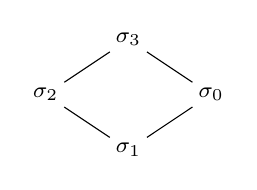
\begin{tikzpicture}[baseline=(current bounding box.center),every node/.style={font=\footnotesize, inner sep=2pt}]
\node (t) at (0,1.4) {$\sigma_3$};
\node (l) at (-1.05,0.7) {$\sigma_2$};
\node (r) at (1.05,0.7) {$\sigma_0$};
\node (b) at (0,0) {$\sigma_1$};
\draw (t)--(l); \draw (t)--(r); \draw (l)--(b); \draw (r)--(b);
\end{tikzpicture}
\]
这里各个 $\sigma_i$ 是 $\mathrm{PS}(\xi)$ 的 Jordan--Hölder 因子；图中各行是它的基座滤过（socle filtration）的层（从图的底部数起），等价地，是余基座滤过（cosocle filtration）的层（从图的顶部数起）；连线表示非平凡的扩张。

写 $\CC_i:=\CC_{\sigma_i}$；我们现在的目标是描述 $\CC_0\cup\CC_1\cup\CC_2\cup\CC_3$，然后描述其 Picard 群。我们首先注意，此并容许开覆盖
\ysrc{319}\begin{equation}\tag{7.7.20}\label{eq:a4-7-7-20}
\begin{aligned}
\{&D(u_0x_0),\;D(v_1y_1),\;D(u_2x_2),\;D(v_3y_3),\;D(v_0x_0)\cup D(u_1y_1),\\
&D(v_1x_1)\cup D(u_2y_2),\;D(v_2x_2)\cup D(u_3y_3),\;D(v_3x_3)\cup D(u_0y_0),\\
&D(v_0y_0)\cup D(u_1x_1)\cup D(v_2y_2)\cup D(u_3x_3)\}.
\end{aligned}
\end{equation}
（这里及下文沿用 $u,v,x,y,a,b$ 的记号，但加下标 $i\in\{0,1,2,3\}$ 以指明变量所属的成分。）以下是这些开子集的显式描述：
\[
D(u_ix_i)=(\GG_m)_{u_i/x_i}\times[\mathbf A^2_{v_i,y_i}/(\GG_m)_{b_i}],\qquad
D(v_iy_i)=[\mathbf A^2_{u_i,x_i}/(\GG_m)_{a_i}]\times(\GG_m)_{v_iy_i};
\]
\[
D(v_ix_i)=\mathbf A^1_{u_i/x_i}\times\mathbf A^1_{v_iy_i},\qquad
D(u_{i+1}y_{i+1})=\mathbf A^1_{x_{i+1}/u_{i+1}}\times\mathbf A^1_{v_{i+1}y_{i+1}},
\]
并且对 $i=0,2$，有
\[
D(v_ix_i)\cup D(u_{i+1}y_{i+1})=\{(u_i/x_i,v_iy_i,v_{i+1}y_{i+1})\mid (u_i/x_i)(v_{i+1}y_{i+1})=0\},
\]
连同等同 $v_iy_i=x_{i+1}/u_{i+1}$；而对 $i=1,3$，有
\[
D(v_ix_i)\cup D(u_{i+1}y_{i+1})=\{(u_i/x_i,v_iy_i,x_{i+1}/u_{i+1})\mid (v_iy_i)(x_{i+1}/u_{i+1})=0\},
\]
连同等同 $u_i/x_i=v_{i+1}y_{i+1}$；最后
\[
\begin{aligned}
& D(v_0y_0)\cup D(u_1x_1)\cup D(v_2y_2)\cup D(u_3x_3)\\
&=[\{(u_0,x_0,v_1,y_3,v_0y_0)\mid u_0v_1=x_0y_3=0,\ v_0y_0\neq0\}/(\GG_m)_{a_0}],
\end{aligned}
\]
其中我们有等同
\[
x_0=y_1,\quad x_2=y_3,\quad u_0=v_3,\quad u_2=v_1,
\]
\[
v_0y_0=x_1/u_1=(v_2y_2)^{-1}=u_3/x_3,\qquad a_0=b_1^{-1}=a_2^{-1}=b_3.
\]
利用开覆盖 (7.7.20)，我们计算
\begin{equation}\tag{7.7.21}\label{eq:a4-7-7-21}
\Gamma(\OO_{\CC_0\cup\CC_1\cup\CC_2\cup\CC_3})=k[v_1y_1,v_3y_3]/(v_1y_1v_3y_3).
\end{equation}
（稍作说明：函数 $v_1y_1$ 在 $\CC_1$ 上良定义，并零延拓到四个成分之并上。类似地，函数 $v_3y_3$ 在 $\CC_3$ 上良定义，也零延拓。）

可以证明存在嵌入
\begin{equation}\tag{7.7.22}\label{eq:a4-7-7-22}
\mathrm{Pic}(\CC_0\cup\CC_1\cup\CC_2\cup\CC_3)\hookrightarrow\Z\times\Z\times\Z\times\Z\times\Z,
\end{equation}
其中各因子分别由 $\mathrm{Pic}(D(v_1y_1))$、$\mathrm{Pic}(D(v_3y_3))$、$\mathrm{Pic}\bigl(D(v_0y_0)\cup D(u_1x_1)\cup D(v_2y_2)\cup D(u_3x_3)\bigr)$、$\mathrm{Pic}(D(u_0x_0))$ 与 $\mathrm{Pic}(D(u_2x_2))$ 给出，态射由限制定义。此嵌入的像等于
\begin{equation}\tag{7.7.23}\label{eq:a4-7-7-23}
\{(j,k,l,m,n)\mid j-k+m-n=0\};
\end{equation}
特别地，$\mathrm{Pic}(\CC_0\cup\CC_1\cup\CC_2\cup\CC_3)\cong\Z^4$。

要精确固定坐标的选取，最简单的办法是描述相应的嵌入
\begin{equation}\tag{7.7.24}\label{eq:a4-7-7-24}
\mathrm{Pic}(\CC_0\cup\CC_1\cup\CC_2\cup\CC_3)\hookrightarrow\mathrm{Pic}(\CC_0)\times\mathrm{Pic}(\CC_1)\times\mathrm{Pic}(\CC_2)\times\mathrm{Pic}(\CC_3);
\end{equation}
\ysrc{320}它由
\begin{equation}\tag{7.7.25}\label{eq:a4-7-7-25}
(j,k,l,m,n)\mapsto\bigl((l,m),(j,-l),(-l,n),(k,l)\bigr)
\end{equation}
给出。

\begin{exam}{7.7.26}\label{thm:a4-7-7-26}
我们有如下 $\OO_{\CC_0\cup\CC_1\cup\CC_2\cup\CC_3}$ 的理想子层图：
\begin{center}
\begin{tikzcd}[row sep=1.05cm, column sep=0.55cm, cells={font=\footnotesize}]
 & \OO_{\CC_0\cup\CC_1\cup\CC_2\cup\CC_3} & & & \\
 & \mathcal I_{\CC_3} \arrow[u, hook, "{\OO_{\CC_3}}"] \arrow[r, equal] & \mathcal I_{\CC_2\cup\CC_3}+\mathcal I_{\CC_0\cup\CC_3} & & \\
\mathcal I_{\CC_2\cup\CC_3} \arrow[ur, hook, "{\OO_{\CC_2}(-1,0)}" pos=0.42] & & \mathcal I_{\CC_0\cup\CC_3} \arrow[ul, hook, "{\OO_{\CC_0}(-1,0)}" pos=0.58] & & \\
 & \mathcal I_{\CC_0\cup\CC_2\cup\CC_3} \arrow[ul, hook] \arrow[ur, hook] \arrow[r, equal] & \mathcal I_{\CC_2\cup\CC_3}\cap\mathcal I_{\CC_0\cup\CC_3} \arrow[r, equal] & v_1y_1\OO_{\CC_0\cup\CC_1\cup\CC_2\cup\CC_3} & \OO_{\CC_1} \arrow[l, hook', "{\sim}" below, "{v_1y_1\cdot}" above]
\end{tikzcd}
\end{center}
其中箭头上的层标号表示相应的余核\tn{底本此句作「where the sheaf labels on the arrows are indicate the corresponding cokernel」，其中「are indicate」语法不谐；译文按原意处理。上下文推断，无外部依据。}。于是可以用如下扩张图描述 $\OO_{\CC_0\cup\CC_1\cup\CC_2\cup\CC_3}$：
\begin{equation}\tag{7.7.27}\label{eq:a4-7-7-27}
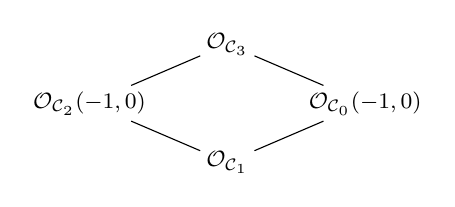
\begin{tikzpicture}[baseline=(current bounding box.center),every node/.style={font=\footnotesize, inner sep=2pt}]
\node (t) at (0,1.5) {$\OO_{\CC_3}$};
\node (l) at (-1.75,0.75) {$\OO_{\CC_2}(-1,0)$};
\node (r) at (1.75,0.75) {$\OO_{\CC_0}(-1,0)$};
\node (b) at (0,0) {$\OO_{\CC_1}$};
\draw (t)--(l); \draw (t)--(r); \draw (l)--(b); \draw (r)--(b);
\end{tikzpicture}
\end{equation}
类似地，我们有图
\begin{center}
\begin{tikzcd}[row sep=1.05cm, column sep=0.55cm, cells={font=\footnotesize}]
 & \OO_{\CC_0\cup\CC_1\cup\CC_2\cup\CC_3} & & & \\
 & \mathcal I_{\CC_1} \arrow[u, hook, "{\OO_{\CC_1}}"] \arrow[r, equal] & \mathcal I_{\CC_0\cup\CC_1}+\mathcal I_{\CC_1\cup\CC_2} & & \\
\mathcal I_{\CC_0\cup\CC_1} \arrow[ur, hook, "{\OO_{\CC_0}(-1,0)}" pos=0.42] & & \mathcal I_{\CC_1\cup\CC_2} \arrow[ul, hook, "{\OO_{\CC_2}(-1,0)}" pos=0.58] & & \\
 & \mathcal I_{\CC_0\cup\CC_1\cup\CC_2} \arrow[ul, hook] \arrow[ur, hook] \arrow[r, equal] & \mathcal I_{\CC_0\cup\CC_1}\cap\mathcal I_{\CC_1\cup\CC_2} \arrow[r, equal] & v_3y_3\OO_{\CC_0\cup\CC_1\cup\CC_2\cup\CC_3} & \OO_{\CC_3} \arrow[l, hook', "{\sim}" below, "{v_3y_3\cdot}" above]
\end{tikzcd}
\end{center}
\ysrc{321}由此可以用如下扩张图描述 $\OO_{\CC_0\cup\CC_1\cup\CC_2\cup\CC_3}$：
\begin{equation}\tag{7.7.28}\label{eq:a4-7-7-28}
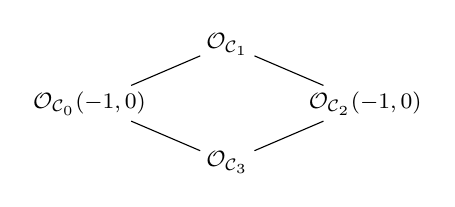
\begin{tikzpicture}[baseline=(current bounding box.center),every node/.style={font=\footnotesize, inner sep=2pt}]
\node (t) at (0,1.5) {$\OO_{\CC_1}$};
\node (l) at (-1.75,0.75) {$\OO_{\CC_0}(-1,0)$};
\node (r) at (1.75,0.75) {$\OO_{\CC_2}(-1,0)$};
\node (b) at (0,0) {$\OO_{\CC_3}$};
\draw (t)--(l); \draw (t)--(r); \draw (l)--(b); \draw (r)--(b);
\end{tikzpicture}
\end{equation}
\end{exam}

\begin{exam}{7.7.29}\label{thm:a4-7-7-29}
我们还有如下 $\OO_{\CC_0\cup\CC_1\cup\CC_2\cup\CC_3}$ 的理想子层图，即
\begin{center}
\begin{tikzcd}[row sep=1.05cm, column sep=0.55cm, cells={font=\footnotesize}]
 & \OO_{\CC_0\cup\CC_1\cup\CC_2\cup\CC_3} & & & \\
 & \mathcal I_{\CC_0} \arrow[u, hook, "{\OO_{\CC_0}}"] \arrow[r, equal] & \mathcal I_{\CC_0\cup\CC_3}+\mathcal I_{\CC_0\cup\CC_1} & & \\
\mathcal I_{\CC_0\cup\CC_3} \arrow[ur, hook, "{\OO_{\CC_3}(0,1)}" pos=0.42] & & \mathcal I_{\CC_0\cup\CC_1} \arrow[ul, hook, "{\OO_{\CC_1}(0,-1)}" pos=0.58] & & \\
 & \mathcal I_{\CC_0\cup\CC_1\cup\CC_3} \arrow[ul, hook] \arrow[ur, hook] \arrow[r, equal] & \mathcal I_{\CC_0\cup\CC_3}\cap\mathcal I_{\CC_0\cup\CC_1} & \OO_{\CC_2}(-2,0) \arrow[l, hook', "{\sim}" below] & 
\end{tikzcd}
\end{center}
与
\begin{center}
\begin{tikzcd}[row sep=1.05cm, column sep=0.55cm, cells={font=\footnotesize}]
 & \OO_{\CC_0\cup\CC_1\cup\CC_2\cup\CC_3} & & & \\
 & \mathcal I_{\CC_2} \arrow[u, hook, "{\OO_{\CC_2}}"] \arrow[r, equal] & \mathcal I_{\CC_1\cup\CC_2}+\mathcal I_{\CC_2\cup\CC_3} & & \\
\mathcal I_{\CC_1\cup\CC_2} \arrow[ur, hook, "{\OO_{\CC_1}(0,1)}" pos=0.42] & & \mathcal I_{\CC_2\cup\CC_3} \arrow[ul, hook, "{\OO_{\CC_3}(0,-1)}" pos=0.58] & & \\
 & \mathcal I_{\CC_1\cup\CC_2\cup\CC_3} \arrow[ul, hook] \arrow[ur, hook] \arrow[r, equal] & \mathcal I_{\CC_1\cup\CC_2}\cap\mathcal I_{\CC_2\cup\CC_3} & \OO_{\CC_0}(-2,0) \arrow[l, hook', "{\sim}" below] & 
\end{tikzcd}
\end{center}
由此可以用如下扩张图描述 $\OO_{\CC_0\cup\CC_1\cup\CC_2\cup\CC_3}$：
\begin{equation}\tag{7.7.30}\label{eq:a4-7-7-30}
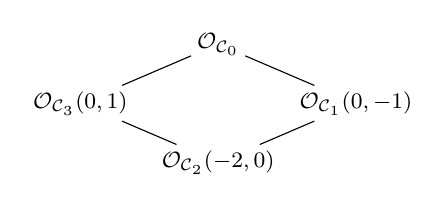
\begin{tikzpicture}[baseline=(current bounding box.center),every node/.style={font=\footnotesize, inner sep=2pt}]
\node (t) at (0,1.5) {$\OO_{\CC_0}$};
\node (l) at (-1.75,0.75) {$\OO_{\CC_3}(0,1)$};
\node (r) at (1.75,0.75) {$\OO_{\CC_1}(0,-1)$};
\node (b) at (0,0) {$\OO_{\CC_2}(-2,0)$};
\draw (t)--(l); \draw (t)--(r); \draw (l)--(b); \draw (r)--(b);
\end{tikzpicture}
\end{equation}
\ysrc{322}与
\begin{equation}\tag{7.7.31}\label{eq:a4-7-7-31}
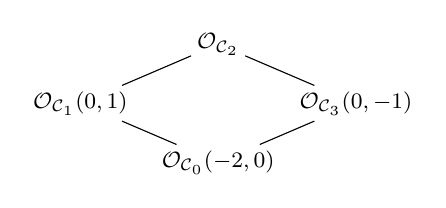
\begin{tikzpicture}[baseline=(current bounding box.center),every node/.style={font=\footnotesize, inner sep=2pt}]
\node (t) at (0,1.5) {$\OO_{\CC_2}$};
\node (l) at (-1.75,0.75) {$\OO_{\CC_1}(0,1)$};
\node (r) at (1.75,0.75) {$\OO_{\CC_3}(0,-1)$};
\node (b) at (0,0) {$\OO_{\CC_0}(-2,0)$};
\draw (t)--(l); \draw (t)--(r); \draw (l)--(b); \draw (r)--(b);
\end{tikzpicture}
\end{equation}
\end{exam}

现在我们解释上述计算的表示论含义。我们写 $U:=\mathrm{PS}(\xi)$，并回忆用其 Jordan--Hölder 因子对 $U$ 的描述
\begin{equation}\tag{7.7.32}\label{eq:a4-7-7-32}
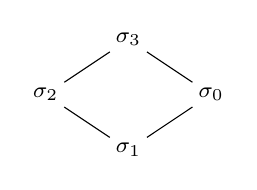
\begin{tikzpicture}[baseline=(current bounding box.center),every node/.style={font=\footnotesize, inner sep=2pt}]
\node (t) at (0,1.4) {$\sigma_3$};
\node (l) at (-1.05,0.7) {$\sigma_2$};
\node (r) at (1.05,0.7) {$\sigma_0$};
\node (b) at (0,0) {$\sigma_1$};
\draw (t)--(l); \draw (t)--(r); \draw (l)--(b); \draw (r)--(b);
\end{tikzpicture}
\end{equation}
于是定义
\[
\mathfrak A(c\text{-}\mathrm{Ind}^G_{KZ}U):=\OO_{\CC_0\cup\CC_1\cup\CC_2\cup\CC_3}(-1,-1,0,0,0),
\]
其中扭按嵌入 (7.7.22) 来理解；注意 $-1-(-1)+0=0=0$\tn{底本此处作 $-1-(-1)+0=0=0$；按 (7.7.23) 的约束 $j-k+m-n=0$，此式应为 $-1-(-1)+0-0=0$，疑排版时漏掉 $-0$；译文照录原文。上下文推断，无外部依据。}，因此 (7.7.23) 的约束得到满足。若对图 (7.7.27) 作相应的扭，并计入 (7.7.25) 的公式，则得到图
\begin{equation}\tag{7.7.33}\label{eq:a4-7-7-33}
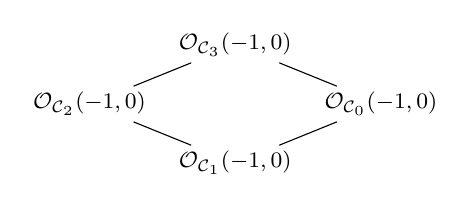
\begin{tikzpicture}[baseline=(current bounding box.center),every node/.style={font=\footnotesize, inner sep=2pt}]
\node (t) at (0,1.5) {$\OO_{\CC_3}(-1,0)$};
\node (l) at (-1.85,0.75) {$\OO_{\CC_2}(-1,0)$};
\node (r) at (1.85,0.75) {$\OO_{\CC_0}(-1,0)$};
\node (b) at (0,0) {$\OO_{\CC_1}(-1,0)$};
\draw (t)--(l); \draw (t)--(r); \draw (l)--(b); \draw (r)--(b);
\end{tikzpicture}
\end{equation}
它表明我们的定义与 $\mathfrak A$ 的函子性以及图 (7.7.32) 相容。

若改为诱导特征 $\xi^s$（$\xi$ 的非平凡 Weyl 群共轭），则得到表示 $U^s:=\mathrm{PS}(\xi^s)$，它可由如下扩张图描述：
\begin{equation}\tag{7.7.34}\label{eq:a4-7-7-34}
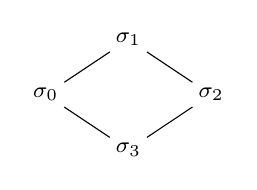
\begin{tikzpicture}[baseline=(current bounding box.center),every node/.style={font=\footnotesize, inner sep=2pt}]
\node (t) at (0,1.4) {$\sigma_1$};
\node (l) at (-1.05,0.7) {$\sigma_0$};
\node (r) at (1.05,0.7) {$\sigma_2$};
\node (b) at (0,0) {$\sigma_3$};
\draw (t)--(l); \draw (t)--(r); \draw (l)--(b); \draw (r)--(b);
\end{tikzpicture}
\end{equation}

% 本片止于印刷页 322 页末（§7.7.19）。续片自 PDF 336 页（印刷页 323）起。

% ch-a4-14.tex —— 第 4 篇（Emerton–Gee–Hellmann）续片，底本 PDF 336–347 = 印刷页 323–334

\ysrc{323}
虽然 $U$ 与 $U^s$ 作为 $\mathrm{GL}_2(\F_{p^2})$ 的表示不同构，但它们到 $\mathrm{GL}_2(\Q_{p^2})$ 的紧诱导同构（经由同构 (7.7.8)），因此我们同样有
\[
\mathfrak A\bigl(c\text{-}\mathrm{Ind}_{KZ}^GU^s\bigr)=\OO_{C_0\cup C_1\cup C_2\cup C_3}(-1,-1,0,0,0).
\]
注意：若以 $(-1,-1,0,0,0)$ 对图 (7.7.28) 作扭，便得到图
\begin{equation}\tag{7.7.35}
\begin{tikzcd}[column sep=large,row sep=large]
& \OO_{C_1}(-1,0)\arrow[dl,no head]\arrow[dr,no head] & \\
\OO_{C_0}(-1,0)\arrow[dr,no head] & & \OO_{C_2}(-1,0)\arrow[dl,no head]\\
& \OO_{C_3}(-1,0) &
\end{tikzcd}
\end{equation}
这验证了 $\mathfrak A$ 作用于图 (7.7.34) 时的函子性。

复合映射
\[
c\text{-}\mathrm{Ind}_{KZ}^G\sigma_1\ra c\text{-}\mathrm{Ind}_{KZ}^GU\isom c\text{-}\mathrm{Ind}_{KZ}^GU^s\ra c\text{-}\mathrm{Ind}_{KZ}^G\sigma_1
\]
已知与 Hecke 算子 $T$ 重合。考察例 7.7.26 中的诸图可知，该映射由乘以 $v_1y_1$ 给出，而这正是 $\mathfrak A(T)$。与此计算相关，我们指出：(7.7.21) 与 $\mathfrak A$ 的全忠实性、以及 $c\text{-}\mathrm{Ind}_{KZ}^GU$ 的自同态环的已知结构相容。

众所周知，通过约化整主级数中的格，我们还能得到 $\mathrm{GL}_2(\F_q)$ 的表示 $V$ 与 $W$，它们可分别用扩展图（extension diagram）
\begin{equation}\tag{7.7.36}
\begin{tikzcd}[column sep=large,row sep=large]
& \sigma_0\arrow[dl,no head]\arrow[dr,no head] & \\
\sigma_3\arrow[dr,no head] & & \sigma_1\arrow[dl,no head]\\
& \sigma_2 &
\end{tikzcd}
\end{equation}
与
\begin{equation}\tag{7.7.37}
\begin{tikzcd}[column sep=large,row sep=large]
& \sigma_2\arrow[dl,no head]\arrow[dr,no head] & \\
\sigma_1\arrow[dr,no head] & & \sigma_3\arrow[dl,no head]\\
& \sigma_0 &
\end{tikzcd}
\end{equation}
描述。我们定义
\[
\mathfrak A\bigl(c\text{-}\mathrm{Ind}_{KZ}^GV\bigr):=\OO_{C_0\cup C_1\cup C_2\cup C_3}(-1,-1,-1,0,0)
\]
以及
\[
\mathfrak A\bigl(c\text{-}\mathrm{Ind}_{KZ}^GW\bigr):=\OO_{C_0\cup C_1\cup C_2\cup C_3}(-1,-1,1,0,0).
\]

\ysrc{324}
然后分别以 $(-1,-1,-1,0,0)$ 与 $(-1,-1,1,0,0)$ 对图 (7.7.30) 与 (7.7.31) 作扭，得到图
\begin{equation}\tag{7.7.38}
\begin{tikzcd}[column sep=large,row sep=large]
& \OO_{C_0}(-1,0)\arrow[dl,no head]\arrow[dr,no head] & \\
\OO_{C_3}(-1,0)\arrow[dr,no head] & & \OO_{C_1}(-1,0)\arrow[dl,no head]\\
& \OO_{C_2}(-1,0) &
\end{tikzcd}
\end{equation}
与
\begin{equation}\tag{7.7.39}
\begin{tikzcd}[column sep=large,row sep=large]
& \OO_{C_2}(-1,0)\arrow[dl,no head]\arrow[dr,no head] & \\
\OO_{C_1}(-1,0)\arrow[dr,no head] & & \OO_{C_3}(-1,0)\arrow[dl,no head]\\
& \OO_{C_0}(-1,0) &
\end{tikzcd}
\end{equation}
这验证了 $\mathfrak A$ 作用于 (7.7.36) 与 (7.7.37) 时的函子性。

\subsubsection*{7.7.40.\quad 四分支之并——情形二（尖点）}
此情形的计算与主级数情形的计算类似。不过，对驯顺尖点型（tame cuspidal type）而言，并不存在优先的格。其约化（一般地）含四个权 $\sigma_0$、$\sigma_1$、$\sigma_2$ 与 $\sigma_3$，每个重数一，并且可以安排它们出现在扩展图
\[
\begin{tikzcd}[column sep=large,row sep=large]
& \sigma_0\arrow[dl,no head]\arrow[dr,no head] & \\
\sigma_3\arrow[dr,no head] & & \sigma_1\arrow[dl,no head]\\
& \sigma_2 &
\end{tikzcd}
\]
中，更一般地出现在该图的任一循环置换中。

在对权作适当标号之后，并 $C_{\sigma_0}\cup C_{\sigma_1}\cup C_{\sigma_2}\cup C_{\sigma_3}$ 容许开覆盖
\begin{equation}\tag{7.7.41}
\begin{aligned}
\bigl\{&D(v_0x_0),\ D(u_1y_1),\ D(v_2x_2),\ D(u_3y_3),\ D(v_0y_0)\cup D(u_1x_1),\\
&D(v_1y_1)\cup D(u_2x_2),\ D(v_2y_2)\cup D(u_3x_3),\ D(v_3y_3)\cup D(u_0x_0),\\
&D(u_0y_0)\cup D(v_1x_1)\cup D(u_2y_2)\cup D(v_3x_3)\bigr\}.
\end{aligned}
\end{equation}
我们有
\[
\begin{aligned}
D(u_iy_i)&=\mathbf A^1_{x_i/u_i}\times\mathbf A^1_{v_iy_i},\\
D(v_ix_i)&=\mathbf A^1_{u_i/x_i}\times\mathbf A^1_{v_iy_i},\\
D(u_ix_i)&=(\mathbf G_m)_{x_i/u_i}\times\bigl[\mathbf A^2_{v_i,y_i}/(\mathbf G_m)_{b_i}\bigr],\\
D(v_iy_i)&=\bigl[\mathbf A^2_{u_i,x_i}/(\mathbf G_m)_{a_i}\bigr]\times(\mathbf G_m)_{v_iy_i},
\end{aligned}
\]

\ysrc{325}
且对 $i=0,2$，有
\[
D(v_iy_i)\cup D(u_{i+1}x_{i+1})=\Bigl[\bigl\{(u_i,x_i,v_iy_i,y_{i+1})\bigm| v_iy_i\neq0,\ x_iy_{i+1}=0\bigr\}\big/(\mathbf G_m)_{a_i}\Bigr],
\]
其中等同关系为 $u_i=v_{i+1}$、$v_iy_i=u_{i+1}/x_{i+1}$ 与 $a_i=b_{i+1}$；而对 $i=1,3$，有
\[
D(v_iy_i)\cup D(u_{i+1}x_{i+1})=\Bigl[\bigl\{(u_i,x_i,v_iy_i,v_{i+1})\bigm| v_iy_i\neq0,\ u_iv_{i+1}=0\bigr\}\big/(\mathbf G_m)_{a_i}\Bigr],
\]
其中等同关系为 $x_i=y_{i+1}$、$v_iy_i=x_{i+1}/u_{i+1}$ 与 $a_i=b_{i+1}^{-1}$；最后
\[
\begin{aligned}
&D(u_0y_0)\cup D(v_1x_1)\cup D(u_2y_2)\cup D(v_3x_3)\\
&\qquad=\bigl\{(v_0y_0,v_1y_1,v_2y_2,v_3y_3)\bigm|(v_0y_0)(v_2y_2)=(v_1y_1)(v_3y_2)=0\bigr\},
\end{aligned}
\]
其中等同关系为 $x_0/u_0=v_3y_3$、$u_1/x_1=v_0y_0$、$x_2/u_2=v_1y_1$ 与 $u_3/x_3=v_2y_2$\tn{底本此处作 $(v_1y_1)(v_3y_2)=0$；按本段末尾的等同关系 $x_0/u_0=v_3y_3$ （以及 $u_3/x_3=v_2y_2$）所体现的模式，第二项应为 $v_3y_3$，疑为底本笔误。译文照录原文。}。

利用开覆盖 (7.7.41)，我们计算得
\begin{equation}\tag{7.7.42}
\Gamma\bigl(\OO_{C_0\cup C_1\cup C_2\cup C_3}\bigr)=k.
\end{equation}
我们还计算得
\[
\mathrm{Pic}\bigl(C_0\cup C_1\cup C_2\cup C_3\bigr)=\Z\times\Z\times\Z\times\Z,
\]
其中各因子依次由 $\mathrm{Pic}\bigl(D(v_2y_2)\cup D(u_3x_3)\bigr)$、$\mathrm{Pic}\bigl(D(v_1y_1)\cup D(u_2x_2)\bigr)$、$\mathrm{Pic}\bigl(D(v_0y_0)\cup D(u_1x_1)\bigr)$ 与 $\mathrm{Pic}\bigl(D(v_3y_3)\cup D(u_0x_0)\bigr)$ 给出。我们通过描述嵌入
\begin{equation}\tag{7.7.43}
\mathrm{Pic}\bigl(C_0\cup C_1\cup C_2\cup C_3\bigr)\into\mathrm{Pic}(C_0)\times\mathrm{Pic}(C_1)\times\mathrm{Pic}(C_2)\times\mathrm{Pic}(C_3)
\end{equation}
来固定坐标的选取；该嵌入由
\begin{equation}\tag{7.7.44}
(k,l,m,n)\mapsto\bigl((m,n),(-l,m),(k,l),(-n,k)\bigr)
\end{equation}
给出。

\begin{exam}{7.7.45}\label{exam:a4-7-7-45}
我们有下列 $\OO_{C_0\cup C_1\cup C_2\cup C_3}$ 的理想子层（ideal subsheaf）图：
{\small
\[
\begin{tikzcd}[column sep=tiny,row sep=large]
 & \OO_{C_0\cup C_1\cup C_2\cup C_3} & & \\
 & \mathcal I_{C_0}\arrow[u,"\OO_{C_0}"]\arrow[r,equal,no head] & \mathcal I_{C_0\cup C_3}+\mathcal I_{C_0\cup C_1} & \\
 \mathcal I_{C_0\cup C_3}\arrow[ur,hook,"{\OO_{C_3}(-1,0)}"] & & \mathcal I_{C_0\cup C_3}\arrow[ul,hook,"{\OO_{C_1}(0,1)}"'] & \\
 & \mathcal I_{C_0\cup C_1\cup C_3}\arrow[ul,hook]\arrow[rr,equal,no head] & & \mathcal I_{C_0\cup C_3}\cap\mathcal I_{C_0\cup C_1}\arrow[ul,hook] & & \OO_{C_2}(-1,-1)\arrow[ll,"\sim"]
\end{tikzcd}
\]}
\tn{底本此图右中与左中的两个节点都印作 $\mathcal I_{C_0\cup C_3}$；按本图其余三幅（以及下方求交的写法 $\mathcal I_{C_0\cup C_3}\cap\mathcal I_{C_0\cup C_1}$）的模式，右中节点应为 $\mathcal I_{C_0\cup C_1}$。译文照录原文。}
\ysrc{326}
{\small
\[
\begin{tikzcd}[column sep=tiny,row sep=large]
 & \OO_{C_0\cup C_1\cup C_2\cup C_3} & & \\
 & \mathcal I_{C_1}\arrow[u,"\OO_{C_1}"]\arrow[r,equal,no head] & \mathcal I_{C_0\cup C_1}+\mathcal I_{C_1\cup C_2} & \\
 \mathcal I_{C_0\cup C_1}\arrow[ur,hook,"{\OO_{C_0}(-1,0)}"] & & \mathcal I_{C_1\cup C_2}\arrow[ul,hook,"{\OO_{C_2}(0,-1)}"'] & \\
 & \mathcal I_{C_0\cup C_1\cup C_2}\arrow[ul,hook]\arrow[rr,equal,no head] & & \mathcal I_{C_0\cup C_1}\cap\mathcal I_{C_1\cup C_2}\arrow[ul,hook] & & \OO_{C_3}(-1,1)\arrow[ll,"\sim"]
\end{tikzcd}
\]}
{\small
\[
\begin{tikzcd}[column sep=tiny,row sep=large]
 & \OO_{C_0\cup C_1\cup C_2\cup C_3} & & \\
 & \mathcal I_{C_2}\arrow[u,"\OO_{C_2}"]\arrow[r,equal,no head] & \mathcal I_{C_1\cup C_2}+\mathcal I_{C_2\cup C_3} & \\
 \mathcal I_{C_1\cup C_2}\arrow[ur,hook,"{\OO_{C_1}(-1,0)}"] & & \mathcal I_{C_2\cup C_3}\arrow[ul,hook,"{\OO_{C_3}(0,1)}"'] & \\
 & \mathcal I_{C_1\cup C_2\cup C_3}\arrow[ul,hook]\arrow[rr,equal,no head] & & \mathcal I_{C_1\cup C_2}\cap\mathcal I_{C_2\cup C_3}\arrow[ul,hook] & & \OO_{C_0}(-1,-1)\arrow[ll,"\sim"]
\end{tikzcd}
\]}
{\small
\[
\begin{tikzcd}[column sep=tiny,row sep=large]
 & \OO_{C_0\cup C_1\cup C_2\cup C_3} & & \\
 & \mathcal I_{C_3}\arrow[u,"\OO_{C_3}"]\arrow[r,equal,no head] & \mathcal I_{C_2\cup C_3}+\mathcal I_{C_0\cup C_3} & \\
 \mathcal I_{C_2\cup C_3}\arrow[ur,hook,"{\OO_{C_2}(-1,0)}"] & & \mathcal I_{C_0\cup C_3}\arrow[ul,hook,"{\OO_{C_0}(0,-1)}"'] & \\
 & \mathcal I_{C_0\cup C_2\cup C_3}\arrow[ul,hook]\arrow[rr,equal,no head] & & \mathcal I_{C_2\cup C_3}\cap\mathcal I_{C_0\cup C_3}\arrow[ul,hook] & & \OO_{C_1}(-1,1)\arrow[ll,"\sim"]
\end{tikzcd}
\]}
\end{exam}

下列表示（用其扩展图描述）作为尖点型中格的约化出现：
\begin{equation}\tag{7.7.46}
\begin{tikzcd}[column sep=large,row sep=large]
& \sigma_0\arrow[dl,no head]\arrow[dr,no head] & \\
\sigma_3\arrow[dr,no head] & & \sigma_1\arrow[dl,no head]\\
& \sigma_2 &
\end{tikzcd}
\end{equation}

\ysrc{327}
\begin{equation}\tag{7.7.47}
\begin{tikzcd}[column sep=large,row sep=large]
& \sigma_1\arrow[dl,no head]\arrow[dr,no head] & \\
\sigma_0\arrow[dr,no head] & & \sigma_2\arrow[dl,no head]\\
& \sigma_3 &
\end{tikzcd}
\end{equation}
\begin{equation}\tag{7.7.48}
\begin{tikzcd}[column sep=large,row sep=large]
& \sigma_2\arrow[dl,no head]\arrow[dr,no head] & \\
\sigma_1\arrow[dr,no head] & & \sigma_3\arrow[dl,no head]\\
& \sigma_0 &
\end{tikzcd}
\end{equation}
以及
\begin{equation}\tag{7.7.49}
\begin{tikzcd}[column sep=large,row sep=large]
& \sigma_3\arrow[dl,no head]\arrow[dr,no head] & \\
\sigma_2\arrow[dr,no head] & & \sigma_0\arrow[dl,no head]\\
& \sigma_1 &
\end{tikzcd}
\end{equation}
相应的 $\mathfrak A$ 取值为
\[
\begin{aligned}
&\OO_{C_0\cup C_1\cup C_2\cup C_3}(0,1,-1,0),\quad
 \OO_{C_0\cup C_1\cup C_2\cup C_3}(-1,1,0,0),\\
&\OO_{C_0\cup C_1\cup C_2\cup C_3}(-1,0,0,1)\quad\text{与}\quad
 \OO_{C_0\cup C_1\cup C_2\cup C_3}(0,0,-1,1)\text{。}
\end{aligned}
\]若以相应的扭对例 7.7.45 中的每个图作扭（并用公式 (7.7.44) 计算），我们就得到一个由诸 $\mathfrak A(\sigma_i)$ 按适当次序拼成的扩展图；这依次验证了 $\mathfrak A$ 在诸图 (7.7.46)、(7.7.47)、(7.7.48) 与 (7.7.49) 上的函子性。

\subsubsection*{7.7.50.\quad 一个非紧诱导的例子}
同构 $c\text{-}\mathrm{Ind}_{KZ}^G\ol{\mathrm{PS}}(\xi)\isom c\text{-}\mathrm{Ind}_{KZ}^G\ol{\mathrm{PS}}(\xi^s)$ 使我们能构造一个有趣的表示。（这里 $\ol{\mathrm{PS}}(\xi)$ 就是 §7.7.19 中记作 $U$ 的表示，$\ol{\mathrm{PS}}(\xi^s)$ 是记作 $U^s$ 的表示。）若以 $\sigma_\xi$ 记 $\ol{\mathrm{PS}}(\xi)$ 的基座（socle），以 $\sigma_{\xi^s}$ 记 $\ol{\mathrm{PS}}(\xi^s)$ 的基座，则有嵌入
\[
c\text{-}\mathrm{Ind}_{KZ}^G\sigma_\xi\into c\text{-}\mathrm{Ind}_{KZ}^G\ol{\mathrm{PS}}(\xi)
\quad\text{与}\quad
c\text{-}\mathrm{Ind}_{KZ}^G\sigma_{\xi^s}\into c\text{-}\mathrm{Ind}_{KZ}^G\ol{\mathrm{PS}}(\xi^s)\isom c\text{-}\mathrm{Ind}_{KZ}^G\ol{\mathrm{PS}}(\xi),
\]
从而诱导出
\[
c\text{-}\mathrm{Ind}_{KZ}^G\sigma_\xi\oplus c\text{-}\mathrm{Ind}_{KZ}^G\sigma_{\xi^s}\into c\text{-}\mathrm{Ind}_{KZ}^G\ol{\mathrm{PS}}(\xi).
\]
定义 $\Pi$ 为该嵌入的余核。

利用 §7.7.19 的计算，我们可以算出 $\mathfrak A(\Pi)$。事实上，注意在该讨论的记号下 $\sigma_\xi$ 与 $\sigma_{\xi^s}$ 可以取为 $\sigma_1$ 与 $\sigma_3$，我们发现 $\mathfrak A(\Pi)$ 是嵌入
\[
\OO_{C_1}(-1,0)\oplus\OO_{C_3}(-1,0)\into\OO_{C_0\cup C_1\cup C_2\cup C_3}(-1,-1,0,0,0)
\]
的余核。

\ysrc{328}
该嵌入的像可等同于理想子层 $\mathcal I_{C_0\cup C_2}$ 经 $(-1,-1,0,0,0)$ 的扭，并且可以算出 $\mathfrak A(\Pi)$ 是 $C_0\cup C_2$ 上的某个可逆层。（特别地，它不是 Cohen--Macaulay 的。）

\subsubsection*{7.7.51.\quad 一个例子——权循环}
在 2006 年的 AIM 会议上，与会者找到了一个论证，它后来被称为「权循环」（weight cycling）。其原始形式如下。（欲知更多细节，感兴趣的读者可参看当时的报告 \url{https://aimath.org/WWN/padicmodularity/emertonreport.pdf} 与 \url{https://www.ma.ic.ac.uk/~buzzard/maths/research/notes/notes_on_mod_p_local_langlands.pdf}。）

\begin{prop}{7.7.52}\label{prop:a4-7-7-52}
设 $\pi'$ 是 $\mathrm{GL}_2(\Q_{p^2})$ 的表示，满足下列性质：
\begin{enumerate}[(1)]
\item $\pi'$ 的 $K$-基座（$K$-socle）的各组成因子（constituent）都在某个充分一般的尖点型（cuspidal type）$\tau$ 的约化之中；
\item $\pi'$ 的 $K$-基座的每个组成因子都以重数一出现；
\item $\pi'$ 的 $K$-基座的每个组成因子都是超奇异的。
\end{enumerate}
则 $\pi'$ 有一个（必然不可约的）子表示 $\pi$，具有下列性质：
\begin{enumerate}[(a)]
\item $\pi$ 有中心特征（central character）；
\item $\pi'$ 的每个 $G$-子表示都含 $\pi$；
\item $\pi$ 的 $K$-基座与 $\pi'$ 的 $K$-基座相同；
\item $\tau$ 的约化的四个组成因子都实际出现在 $\pi'$ 与 $\pi$ 的公共 $K$-基座中。
\end{enumerate}
\end{prop}

\begin{proof}
$\pi'$ 的任一 $G$-子表示都至少含 $\pi'$ 的 $K$-基座的一个组成因子，从而含该组成因子生成的 $G$-子表示。因此，只要能证明：由其中任一组成因子生成的 $G$-子表示 $\pi$ 含所有这些组成因子——也就是说，只要能证明 $\pi$ 满足 (c)——我们也就证明了 $\pi$ 与初始所选取的生成组成因子无关，从而 $\pi$ 也满足条件 (b)。（而 $\pi$ 满足 (b) 这一事实蕴含它不可约。）

于是我们转而证明 $\pi$ 确实满足 (c)。在此过程中，我们还将证明它满足 (a) 与 (d)。

以 $\sigma_0$ 记 $\tau$ 的约化中出现的那个选定的组成因子，它出现在 $\pi'$ 的 $K$-基座中并生成 $\pi$。由于 $\sigma_0$ 在 $\pi$ 的 $K$-基座中以重数一出现，$G$ 的中心 $Z$ 通过某个特征作用在 $\sigma_0$ 上，从而也通过该特征作用在 $\sigma_0$ 生成的表示 $\pi$ 上。这就证明了 (a)。

回忆 $\sigma_0$ 是 $\tau$ 的约化中出现的权之一，于是我们把 $\tau$ 的约化中其余的权标为 $\sigma_1$、$\sigma_2$、$\sigma_3$。由于 $\tau$ 作为 $K$ 的表示有中心特征，每个 $\sigma_i$ 作为 $K$ 的表示也有中心特征，且这些特征都相同（它们就是 $\tau$ 的中心特征的约化）。特别地，$\pi$ 的中心特征与诸 $\sigma_i$ 的中心特征相容（即前者的限制到 $K\cap Z$ 与后者一致），因此我们可以并且确实把每个 $\sigma_i$ 延拓为 $KZ$ 的表示，让 $Z$ 通过 $\pi$ 的中心特征作用。

于是我们可以选取标号，使得对每个 $i=0,\dots,3$，都有一个嵌入（最初由 Pa\v{s}k\={u}nas 构造）
\begin{equation}\tag{7.7.53}
c\text{-}\mathrm{Ind}_{KZ}^G\sigma_{i+1}\oplus c\text{-}\mathrm{Ind}_{KZ}^G\sigma'_{i+1}\into c\text{-}\mathrm{Ind}_{KZ}^G\sigma_i/T,
\end{equation}

\ysrc{329}
其中 $i+1$ 按模 $4$ 计算，而 $\sigma'_{i+1}$ 是另一个 Serre 权，它不同构于任何 $\sigma_j$（$j=0,\dots,3$）。（关于这一点的稍详细说明，见下文注 7.7.54。）

以 $\pi'(\sigma_i)$ 记 (7.7.53) 的余核。一个基本事实是 $\pi'(\sigma_i)=\pi'(\sigma_i^{(s)})$，其中 $\sigma_i^{(s)}$ 记这样的 Serre 权：其最高权由 $\sigma_i$ 的最高权经 Weyl 群的对合 $s$ 作用而得。特别地，$\pi'(\sigma_i)$ 不仅是 $c\text{-}\mathrm{Ind}_{KZ}^G\sigma_i$ 的商，也是 $c\text{-}\mathrm{Ind}_{KZ}^G\sigma_i^{(s)}$ 的商。另一个基本事实是：诸 $\sigma_i^{(s)}$（$i=0,\dots,3$）中没有一个同构于任何 $\sigma_j$；也就是说，这些表示都不是 $\tau$ 的约化的组成因子。（同样见下文注 7.7.54。）由我们对 $\pi'$ 的 $K$-基座所作的假设，这意味着任何态射 $c\text{-}\mathrm{Ind}_{KZ}^G\sigma_i^{(s)}\ra\pi'$（对任何 $i$ 值）都必须为零，从而任何态射 $\pi'(\sigma_i)\ra\pi'$ 也必须为零。由于 $\pi\subseteq\pi'$，把 $\pi'$ 换作 $\pi$ 也有同样的结论。

现在考虑由包含 $\sigma_0\subseteq\pi$ 诱导的态射 $c\text{-}\mathrm{Ind}_{KZ}^G\sigma_0\ra\pi$。超奇异的假设蕴含（事实上，大致就意味着）该态射穿过 $c\text{-}\mathrm{Ind}_{KZ}^G\sigma_0/T$。由于它非零（其像含 $\sigma_0$），它必定不穿过 $\pi'(\sigma_i)$，因此它在 (7.7.53) 的定义域上不恒为零。然而它在该定义域的第二个直和项上必定为零（由我们对 $\pi'$ 的 $K$-基座所作的假设），因而它在第一个直和项上非零。于是我们得到一个非零态射 $c\text{-}\mathrm{Ind}_{KZ}^G\sigma_{i+1}\ra\pi$。等价地，我们得到一个嵌入 $\sigma_{i+1}\into\pi$。

如此继续，我们循环过所有权 $\sigma_i$，发现 $\pi'$ 在其 $K$-基座中含所有这些权，而且事实上它们都含于 $\pi$。这就完成了命题的证明。
\end{proof}

\begin{rem}{7.7.54}\label{rem:a4-7-7-54}
这里只想就我们上面用到的关于 Serre 权的事实略作补充：若以 $\chi_i$ 记 $\sigma_i$ 的最高权，则 $\mathrm{PS}(\chi_i)$ 的约化中的权为 $\sigma_i$、$\sigma_{i+1}$、$\sigma'_{i+1}$ 与 $\sigma_i^{(s)}$\tn{底本此处作 $\mathrm{PS}(\chi_i)$，无上横线；而 §7.7.50 中同一表示记作 $\ol{\mathrm{PS}}({\cdot})$。译文照录原文。}。而（充分一般的）尖点型的约化与（充分一般的）主级数型的约化或者没有公共权，或者恰有两个公共权。因此，既然 $\tau$ 的约化含 $\sigma_i$ 与 $\sigma_{i+1}$，它就不含 $\sigma'_{i+1}$ 或 $\sigma_i^{(s)}$。
\end{rem}

\begin{rem}{7.7.55}\label{rem:a4-7-7-55}
2006 年 AIM 与会者的原意，是取 $\pi'$ 为某条志村曲线（Shimura curve）的完备上同调中的 $\mathfrak m$-挠\tn{底本此处作 the completed cohomology of a Shimura curves，冠词与单复数均不顺；疑为 a Shimura curve 或 Shimura curves 之误。译文照录其意。}（其中 $\mathfrak m$ 记某个适当 Hecke 代数的极大理想），来应用命题 7.7.52。此时在适当的「一般性」假设下，命题的假设已由 [Gee11] 得知成立。更近期地，已经证明此时甚至有 $\pi'=\pi$（见 [BHH${}^{+}$21, Cor. 1.3.10]）。2006 年 AIM 会议后不久，Breuil 与 Pa\v{s}k\={u}nas [BP12] 直接构造出了命题 7.7.52 中的不可约容许表示 $\pi$。事实上，他们给出了无穷多个两两不同构的此类表示。
\end{rem}

命题 7.7.52 的证明表明，实际上有一个标量不变量附着于 $\pi'$——或者更确切地说，附着于它的不可约子表示 $\pi$。具体而言，若我们从包含 $\sigma_0\subseteq\pi$ 出发并循环四次，就回到一个嵌入 $\sigma_0\into\pi$；由我们的重数一假设，它必定等于原嵌入的一个非零标量倍。为使这一点良定义，必须把诸嵌入 (7.7.53) 固定下来，而稍加小心就可以做到

\ysrc{330}
（我们将在下文说明如何在应用 $\mathfrak A$ 之后做到这一点），于是得到 $\pi$ 的一个标量不变量。

更确切地说，取定非零标量 $\lambda=\lambda_0\in k^\times$，并令 $i=1,2,3$ 时 $\lambda_i=1$，考虑两步复形
\begin{equation}\tag{7.7.56}
\begin{tikzcd}[column sep=huge,row sep=small]
\displaystyle\bigoplus_{i=0}^{3}\bigl(c\text{-}\mathrm{Ind}_{KZ}^G\sigma_i\oplus c\text{-}\mathrm{Ind}_{KZ}^G\sigma'_i\bigr)\arrow[r] & \displaystyle\bigoplus_{i=0}^{3}c\text{-}\mathrm{Ind}_{KZ}^G\sigma_i/T,
\end{tikzcd}
\end{equation}
其中箭头在直和项 $c\text{-}\mathrm{Ind}_{KZ}^G\sigma_i\oplus c\text{-}\mathrm{Ind}_{KZ}^G\sigma'_i$ 上由
\[
\begin{aligned}
c\text{-}\mathrm{Ind}_{KZ}^G\sigma_i\oplus c\text{-}\mathrm{Ind}_{KZ}\sigma'_i\ni(v,w)\mapsto{}&(v+w,-\lambda_iv\bmod T)\\
&\in c\text{-}\mathrm{Ind}_{KZ}^G\sigma_{i-1}/T\oplus c\text{-}\mathrm{Ind}_{KZ}^G\sigma_i/T
\end{aligned}
\]
这里我们把 $v$ 与 $w$ 看作 $c\text{-}\mathrm{Ind}_{KZ}\sigma_{i-1}/T$ 的元素\tn{底本此处（及紧接其后的两处）作 $c\text{-}\mathrm{Ind}_{KZ}\sigma'_i$、$c\text{-}\mathrm{Ind}_{KZ}\sigma_{i-1}/T$，均缺上标 $G$；他处则作 $c\text{-}\mathrm{Ind}_{KZ}^G$。译文照录原文。}（经由 (7.7.53)）。

\begin{lem}{7.7.57}\label{lem:a4-7-7-57}
(7.7.56) 的箭头是单射。
\end{lem}

\begin{proof}
若核非零，则它有非零的 $K$-基座，于是对某个权 $\sigma'$，存在非零态射 $c\text{-}\mathrm{Ind}_{KZ}^G\sigma'\ra$ 该核。但若
\[
c\text{-}\mathrm{Ind}_{KZ}^G\sigma'\ra\bigoplus_{i=0}^{3}\bigl(c\text{-}\mathrm{Ind}_{KZ}^G\sigma_i\oplus c\text{-}\mathrm{Ind}_{KZ}^G\sigma'_i\bigr)
\]
非零，则 $\sigma'$ 等于某个 $\sigma_i$ 或 $\sigma'_i$（我们假设这些权充分一般），且该态射只是到相应直和项的嵌入。引理于是由下述事实得出：(7.7.56) 的箭头在其定义域的每个直和项上都是单射。
\end{proof}

以 $\Pi_\lambda$ 记 (7.7.56) 的余核。于是给出态射 $\Pi_\lambda\ra\pi$（$\pi$ 为某个其他表示）等价于给出 $\pi$ 中 $\sigma_0$ 的一个拷贝（或事实上任一 $\sigma_i$ 的拷贝），使得命题 7.7.52 的权循环在 $\pi$ 中「奏效」，且相应的标量等于 $\lambda$。

我们可以计算附着于 $\Pi_\lambda$ 的凝聚层（更确切地说，凝聚层复形）。答案依赖于 $\lambda$。事实上，几何使我们能把诸嵌入 (7.7.53) 标准化。具体而言，箭头 $c\text{-}\mathrm{Ind}_{KZ}^G\sigma_{i+1}\ra c\text{-}\mathrm{Ind}_{KZ}^G\sigma_i/T$ 与 $c\text{-}\mathrm{Ind}_{KZ}^G\sigma'_{i+1}\ra c\text{-}\mathrm{Ind}_{KZ}^G\sigma_i/T$ 在凝聚层一侧分别对应箭头 $\OO_{C_{\sigma_{i+1}}}(-1,0)\ra\OO_{C_\sigma}(-1)/(vy)$ 与 $\OO_{C_{\sigma'_{i+1}}}(-1,0)\ra\OO_{C_\sigma}(-1,0)/(vy)$\tn{底本此处前一箭头作 $\OO_{C_\sigma}(-1)/(vy)$，后一箭头作 $\OO_{C_\sigma}(-1,0)/(vy)$；按后者及上下文，前者疑脱 $0$。译文照录原文。}，而我们可以直接取它们为由包含 $C_\sigma^{vy=0}\into C_{\sigma_{i+1}},C_{\sigma'_{i+1}}$ 诱导的限制映射。对态射 (7.7.56) 应用 $\mathfrak A$，并按上述方式解释其中的诸态射，就可以（稍费些力气）显式算出复形 $\mathfrak A(\Pi_\lambda)$。

我们把这计算的结果总结为下述论断，它特别表明 $\lambda=1$ 这个值是特殊的。

\textbf{结论 7.7.58.}
\begin{enumerate}[(1)]
\item $H^0\bigl(\mathfrak A(\Pi_1)\bigr)$ 是支撑在 $x$ 处的摩天楼层（skyscraper），其中 $x$ 是各分支 $C_{\sigma_i}$（$i=0,\dots,3$）相交所得的闭点；而 $H^{-1}\bigl(\mathfrak A(\Pi_1)\bigr)$ 是支撑在 $\bigcup_{i=0}^{3}\bigl(C_{\sigma_i}\cup C_{\sigma'_i}\bigr)$ 上的线丛。
\item 若 $\lambda\neq1$，则 $H^0\bigl(\mathfrak A(\Pi_\lambda)\bigr)=0$，而 $H^{-1}\bigl(\mathfrak A(\Pi_\lambda)\bigr)$ 是支撑在 $C:=\bigcup_{i=0}^{3}\bigl(C_{\sigma_i}\cup C_{\sigma'_i}\bigr)$ 上的无挠层（torsion-free sheaf）。更确切地说，它是 $C\setminus\{x\}$ 上某个线丛推到 $C$ 上的像，该线丛依赖于参数 $\lambda$。
\end{enumerate}
\ysrc{331}
\subsubsection*{7.7.59.\quad 不可约商}
考虑短正合序列
\[
0\ra\mathcal K\ra\Pi_\lambda\ra\pi\ra0
\]
（其中 $\pi$ 是如上所说的不可约容许表示，而 $\mathcal K$ 定义为该满射的核）。过渡到（如今仅为假设性的）层，并注意 $\mathfrak A$ 的振幅为 $[-1,0]$（见注 6.1.28），我们得到长正合序列
\[
\begin{aligned}
0&\ra H^{-1}\bigl(\mathfrak A(\mathcal K)\bigr)\ra H^{-1}\bigl(\mathfrak A(\Pi_\lambda)\bigr)\ra H^{-1}\bigl(\mathfrak A(\pi)\bigr)\\
&\ra H^0\bigl(\mathfrak A(\mathcal K)\bigr)\ra H^0\bigl(\mathfrak A(\Pi_\lambda)\bigr)\ra H^0\bigl(\mathfrak A(\pi)\bigr)\ra0.
\end{aligned}
\]
若 $\lambda\neq1$，则我们得出 $H^0\bigl(\mathfrak A(\pi)\bigr)=0$（因为 $H^0\bigl(\mathfrak A(\Pi_\lambda)\bigr)=0$），从而 $\mathfrak A(\pi)$ 支撑在次数 $-1$ 上。若 $\lambda=1$，则由于 $H^0\bigl(\mathfrak A(\Pi_1)\bigr)$ 是支撑在 $x$ 处的摩天楼层，我们看到 $H^0\bigl(\mathfrak A(\pi)\bigr)$ 或者同样是支撑在 $x$ 处的摩天楼层，或者为 $0$。

另一方面，由于 $\pi$ 不是有限表现的 [Sch15b]，引理 A.4.6 (3) 蕴含 $H^{-1}\bigl(\mathfrak A(\pi)\bigr)$ 不凝聚，无论 $\lambda$ 取何值。

关于层 $H^{-1}\bigl(\mathfrak A(\pi)\bigr)$，我们能说些什么呢？它有一条性质如下：由于对 $\sigma'\neq\sigma_i$（$i=0,\dots,3$）有 $\Hom(c\text{-}\mathrm{Ind}_{KZ}^G\sigma',\pi)=0$\tn{底本此处作「if $\sigma'\neq\sigma_i$ for some $i=0,\dots,3$」，按文意当为「对一切 $i=0,\dots,3$ 皆有 $\sigma'\neq\sigma_i$」。译文照录原文。}，我们发现对任何这样的 $\sigma'$ 都有
\[
\Ext^1\bigl(\OO_{C_{\sigma'}},H^{-1}(\mathfrak A(\pi))\bigr)=0.
\]
若 $\lambda=1$，如上所说的表示 $\pi$（即 $\Pi_\lambda$ 的一个不可约商，其 $K$-基座恰由诸 $\sigma_i$ 构成、每个重数一）也可以通过整体方式构造，即经由定四元数代数与/或志村曲线的完备上同调。（在此情形下 $\lambda$ 必然等于 $1$，这已由 Dotto--Le [DL21] 证明。完备上同调中的表示已被许多作者研究过，其中 Taylor--Wiles 拼接是关键技术；关于已知结果的简要综述，我们请读者参看 [BHH${}^{+}$21] 的引言。）

当 $\pi$ 经由完备上同调构造时，函子 $\mathfrak A$ 与完备上同调之间所期待的关系提示，映射 $H^0\bigl(\mathfrak A(\Pi_1)\bigr)\ra H^0\bigl(\mathfrak A(\pi)\bigr)$ 应当非零，因此至少在此情形下，我们预期 $H^0\bigl(\mathfrak A(\pi)\bigr)$ 等于 $x$ 处的摩天楼层。我们在 §7.8 中进一步探讨层 $\mathfrak A(\pi)$：在那里我们将看到，我们的猜想蕴含不可约表示 $\pi$ 应当由条件 $H^0\bigl(\mathfrak A(\pi)\bigr)\neq0$ 唯一确定（见注 7.8.6）。

\subsection{伴随函子}
回到猜想 6.1.15 的情形，以及连续函子 $\mathfrak A:\Ind D^b_{\mathrm{f.p.}}(\mathrm{sm}\,G)\ra\Ind\Coh(\XX_d)$。由引理 A.4.6 (1)（即伴随函子定理），$\mathfrak A$ 有右伴随 $\mathfrak B:\Ind\Coh(\XX_d)\ra\Ind D^b_{\mathrm{f.p.}}(\mathrm{sm}\,G)$。由同一引理的第 (2) 部分（它适用，因为按假设 $\mathfrak A$ 保持紧对象；见注 6.1.29），我们看到 $\mathfrak B$ 也是连续的。

\begin{rem}{7.8.1}\label{rem:a4-7-8-1}
在注 1.4.6 的设定下（即 Fargues--Scholze 猜想的 $p$-进版本），函子 $\mathfrak A$ 与 $\mathfrak B$ 想必由函子 $i_!$ 与 $i^!$ 诱导，其中 $i$ 是开 stratum $[*/G(F)]\into\Bun_G$ 的包含。
\end{rem}

\ysrc{332}
我们可以用上一节的计算来研究 $\mathrm{PGL}_2(\Q_p)$ 与 $\mathrm{PGL}_2(\Q_{p^2})$ 情形下的函子 $\mathfrak B$。（当然，这并不完全是猜想 6.1.15 的设定，但上述讨论原封不动地适用于这一情形。）这将使我们能把本文的猜想与经由志村曲线上同调研究 $p$-进及 mod $p$ 局部 Langlands 对应的更传统途径联系起来，尤其与下述希望联系起来：可以把每个表示 $\overline{\rho}:\Gal_{\Q_{p^2}}\ra\mathrm{GL}_2(\F_p)$ 与 $\mathrm{GL}_2(\Q_{p^2})$ 的一个特定的容许表示联系起来，而该表示由它出现在与 $\overline{\rho}$ 的某个整体提升相关的任一（也就是说，每一个！）整体背景中而确定（例如见 [Bre10a, Q.\ 3.11]）。我们将在下文注 7.8.6 中回到这一主题。

我们可以借助 $\mathfrak A$ 与 Taylor--Wiles 拼接之间所期待的相容性来研究 $\mathfrak B$ 的预期性质。设 $F/\Q_p$ 任意，$\XX$ 为行列式为 $\varepsilon^{-1}$ 的秩 $2$ $(\phi,\Gamma)$-模构成的叠；并设 $L_\infty$ 为（当 $F\neq\Q_p$ 时是假设性的）pro-凝聚层，它是 $\mathfrak A$ 的核，即
\[
\mathfrak A(\pi):=L_\infty\otimes^L_{\OO[[G]]}\pi.
\]
则伴随函子由
\begin{equation}\tag{7.8.2}
\mathfrak B(\FF):=\mathrm{RHom}_{\mathrm{Pro-}\OO_\XX}(L_\infty,\FF)
\end{equation}
给出。

现在设 $x:\Spec k\ra\XX$ 是有限型点，对应连续表示 $\overline{\rho}:\Gal_F\ra\mathrm{GL}_2(k)$，并设 $f:\Spf R_\infty\ra\XX$ 是由在 $\overline{\rho}$ 的某个整体化处拼接而得的 versal 态射。由注 6.1.31，我们预期 $f^*L_\infty$ 等于拼接模 $M_\infty$。对一般的 $\overline{\rho}$，环 $R_\infty$ 形式光滑，而由 [GN22, Prop. 4.3.1] 以及 [BHH${}^{+}$23, HW22, Wan23] 的结果可得 $M_\infty$ 在 $R_\infty$ 上 pro-平坦（pro-flat）。我们预期它甚至是 pro-自由的。相应地，我们预期可以用下述公式计算 $\mathfrak B(\FF)$：
\[
\begin{aligned}
\mathfrak B(\FF)&=\mathrm{RHom}_{\mathrm{Pro-}\OO_\XX}(L_\infty,\FF)\\
&=R\Gamma\circ\mathcal Hom_{\mathrm{Pro-}\OO_\XX}(L_\infty,\FF)\\
&=R\Gamma\bigl(\XX,\mathcal Hom_{\mathrm{Pro-}\OO_\XX}(L_\infty,\FF)\bigr).
\end{aligned}
\]

记 $G_x=\Aut_{\Gal_F}(\overline{\rho})$。进一步假设 $\overline{\rho}^{\mathrm{ss}}$ 不是纯量（若如上假设 $\overline{\rho}$ 是一般的，则自动如此）；于是当 $\overline{\rho}$ 不可约或非分裂可约时 $G_x=\mu_2$，而当 $\overline{\rho}$ 是两个不同特征标之和时 $G_x=\mathbf G_m$。于是 $x$ 处的剩余带叠（residual gerbe）是仿射浸入\footnote{若 $\overline{\rho}$ 半单，则 $i$ 是闭浸入；否则 $i$ 分解为 $[\Spec k/\mu_2]\xrightarrow{\ \mathrm{open}\ }[\mathbf A^1_k/\mathbf G_m]\xrightarrow{\ \mathrm{closed}\ }\XX$，从而把它表示为仿射浸入的复合。}
\[
i:[\Spec k/G_x]\into\XX,
\]
并且可以构造拟凝聚层 $\delta_x:=i_*\OO_{[\Spec k/G_x]}$。若如上所述 $f:\Spf R_\infty\ra\XX$ 是由 Taylor--Wiles 拼接而得的 $x$ 处的 versal 态射，$\mathfrak m_\infty$ 记 $R_\infty$ 的极大理想，则我们看到
\[
\mathcal Hom_{\mathrm{Pro-}\OO_\XX}(L_\infty,\delta_x)=M_\infty^\vee[\mathfrak m_\infty]
\]
带有某个 $G_x$-作用。（要看出这一点，注意 $L_\infty\otimes_{\OO_\XX}\delta_x=M_\infty/\mathfrak m_\infty M_\infty$ 带有某个 $G_x$-作用，而 $M_\infty/\mathfrak m_\infty M_\infty$ 的连续 $k$-对偶等于 $M_\infty^\vee[\mathfrak m_\infty]$。）注意：按 Taylor--Wiles 拼接对 $M_\infty$ 的构造，$M_\infty^\vee[\mathfrak m_\infty]$ 等于完备上同调中的 $\mathfrak m$-挠，其中 $\mathfrak m$ 是某个

\ysrc{333}
适当 Hecke 代数的极大理想。由于 $G_x$ 线性约化（它等于 $\mu_2$ 或 $\mathbf G_m$ 之一），我们于是看到
\[
\mathfrak B(\delta_x)=\bigl(M_\infty^\vee[\mathfrak m_\infty]\bigr)^{G_x}.
\]
令 $n$ 变化，我们可以通过取值
\[
\mathfrak B\bigl(\delta_x(n)\bigr)=\bigl(M_\infty^\vee[\mathfrak m_\infty](n)\bigr)^{G_x}
\]
还原出整个 $M_\infty^\vee[\mathfrak m_\infty]$。或者，与其逐个考虑各种扭 $\delta_x(n)$，不如令 $g:\Spec k\ra\XX$ 记复合
\[
\Spec k\ra[\Spec k/G_x]\xrightarrow{\ i\ }\XX,
\]
于是我们可以对拟凝聚层 $\Delta_x:=g_*\OO_{\Spec k}$ 应用 $\mathfrak B$。（这是 $x$ 的剩余带叠上对应于 $G_x$ 的正则表示的那个拟凝聚层。）事实上，我们计算得
\[
\begin{aligned}
\mathfrak B(\Delta_x)&=\mathrm{RHom}_{\mathrm{Pro-}\OO_\XX}\bigl(L_\infty,g_*\OO_{\Spec\mathcal F}\bigr)\\
&=\mathrm{RHom}_{\mathrm{Pro-}\OO_{\Spec k}}\bigl(g^*L_\infty,\OO_{\Spec\mathcal F}\bigr)\\
&=\Hom_{\mathrm{cont}}\bigl(M_\infty/\mathfrak m_\infty M_\infty,k\bigr)=M_\infty^\vee[\mathfrak m_\infty].
\end{aligned}
\]
因此 $x\mapsto\mathfrak B(\Delta_x)$ 应当还原出上文提到的、所期待的「传统」mod $p$ 局部 Langlands 对应。由考虑层-Hom $\mathcal Hom_{\mathrm{Pro-}\OO_\XX}(L_\infty,\delta_x)$ 而来的 $M_\infty^\vee[\mathfrak m_\infty]$ 上的 $G_x$-作用，是 mod $p$ Langlands 对应中某种额外的结构；据我们所知，它此前未被考虑过（尽管可以说它隐含在 Breuil 及其合作者在 [Bre11] 与 [BH15] 等文中所表达的思想之中）。

\subsubsection*{7.8.3.\quad 一些例子}
在 $F=\Q_p$ 或 $F=\Q_{p^2}$ 的情形，我们对 $M_\infty^\vee[\mathfrak m]$ 有所了解（前一情形由 M.\,E.\ 的局部--整体相容性定理 [Eme11a]，后一情形由 [BHH${}^{+}$21]），并且对 $G_x$ 如何作用，或已知、或可猜测。我们有下列例子。

\begin{enumerate}[(1)]
\item 若 $F=\Q_p$ 且 $\overline{\rho}=\overline{\chi}_1\oplus\overline{\chi}_2$，并满足 $\overline{\chi}_1\overline{\chi}_2^{-1}\neq\mathrm{triv}$ 或 $\varepsilon^{\pm1}$，则 $M_\infty^\vee[\mathfrak m]$ 是两个不可约主级数表示 $\pi_1\oplus\pi_2$ 的直和，而且事实上，对 $\pi_1,\pi_2$ 的适当排序，有
\[
\mathcal Hom_{\mathrm{Pro-}\OO_\XX}(L_\infty,\delta_x)=\pi_1(1)\oplus\pi_2(-1)
\]
（其中扭表示 $\mathbf G_m$-作用的权；注意表观上的不对称性源于：为了把 $G_x$ 与 $\mathbf G_m$ 等同，需要给 $\overline{\chi}_1$、$\overline{\chi}_2$ 取一种排序）。在此情形 $\Delta_x:=\bigoplus_{n=-\infty}^{\infty}\delta_x(n)$，因此
\[
\mathfrak B(\Delta_x)=\mathfrak B\bigl(\delta_x(-1)\bigr)\oplus\mathfrak B\bigl(\delta_x(1)\bigr)=\pi_1\oplus\pi_2.
\]
若 $\sigma_1,\sigma_2$ 是 $\overline{\rho}$ 的两个 Serre 权（取定一种排序），则我们发现 $(\mathfrak A\circ\mathfrak B)\bigl(\delta_x(-1)\bigr)=\mathfrak A(\pi_1)$ 支撑在 $\XX(\sigma_1)$ 上，而 $(\mathfrak A\circ\mathfrak B)\bigl(\delta_x(1)\bigr)=\mathfrak A(\pi_2)$ 支撑在 $\XX(\sigma_2)$ 上。作为附带说明，我们指出：虽然 $\delta_x$ 的支撑在交 $\XX(\sigma_1)\cap\XX(\sigma_2)$ 上，但这些表示并非如此；表示 $\mathfrak A(\pi_i)$ 支撑在相应分支 $\XX(\sigma_i)$ 中对应于半单化为 $\overline{\rho}$ 的伽罗瓦表示的那个闭轨迹上。因此 $(\mathfrak A\circ\mathfrak B)(\Delta_x)=\mathfrak A(\pi_1)\oplus\mathfrak A(\pi_2)$ 支撑在这两条轨迹之并上，而后者正是所有以 $\overline{\rho}$ 为其半单化的伽罗瓦表示构成的轨迹。

\ysrc{334}
\item 若 $F=\Q_p$ 且 $\overline{\rho}$ 是特征标 $\chi_1$ 与 $\chi_2$ 的非分裂扩张，同样满足 $\chi_1\chi_2^{-1}\neq\mathrm{triv}$ 或 $\varepsilon^{\pm1}$，则 $M_\infty^\vee[\mathfrak m]$ 是例 (1) 中出现的那两个不可约主级数 $\pi_1$ 与 $\pi_2$ 的非分裂扩张，并且
\[
\mathcal Hom_{\mathrm{Pro-}\OO_\XX}(L_\infty,\delta_x)=M_\infty^\vee[\mathfrak m](1),
\]
其中的扭表明 $\mu_2$ 的作用非平凡。在此情形 $\Delta_x:=\delta_x\oplus\delta_x(1)$，因此
\[
\mathfrak B(\Delta_x)=\mathfrak B\bigl(\delta_x(1)\bigr)=M_\infty^\vee[\mathfrak m]
\]
（即 $\pi_1$ 与 $\pi_2$ 的那个非分裂扩张）。此外，$(\mathfrak A\circ\mathfrak B)(\Delta_x)=(\mathfrak A\circ\mathfrak B)\bigl(\delta_x(1)\bigr)$ 是 $\mathfrak A(\pi_1)$ 与 $\mathfrak A(\pi_2)$ 的非分裂扩张，特别地其支撑等于对应于半单化等于 $\chi_1\oplus\chi_2$ 的伽罗瓦表示的那个闭轨迹。

\item 若 $F=\Q_p$ 且 $\overline{\rho}$ 不可约，则 $M_\infty^\vee[\mathfrak m]=\pi$ 是一个超奇异不可约表示，并且
\[
\mathcal Hom_{\mathrm{Pro-}\OO_\XX}(L_\infty,\delta_x)=\pi(1)
\]
（其中的扭表明 $\mu_2$ 的作用非平凡）。与例 (2) 一样，我们有 $\Delta_x:=\delta_x\oplus\delta_x(1)$，因此
\[
\mathfrak B(\Delta_x)=\mathfrak B\bigl(\delta_x(1)\bigr)=\pi,
\]
并且 $(\mathfrak A\circ\mathfrak B)(\Delta_x)=(\mathfrak A\circ\mathfrak B)\bigl(\delta_x(1)\bigr)=\delta_x(1)$。

\item 若 $F=\Q_{p^2}$ 且 $\overline{\rho}=\chi_1\oplus\chi_2$，其中 $\chi_1,\chi_2$ 适当一般，则由 [BHH${}^{+}$21, Cor. 1.3.10] 有 $M_\infty^\vee[\mathfrak m]=\pi_1\oplus\pi\oplus\pi_2$，其中 $\pi_1,\pi_2$ 是显式的不可约主级数表示，而 $\pi$ 是（非显式的！）超奇异不可约表示。我们预期
\[
\mathcal Hom_{\mathrm{Pro-}\OO_\XX}(L_\infty,\delta_x)=\pi_1(2)\oplus\pi\oplus\pi_2(-2).
\]
假设此式成立，我们看到
\[
\mathfrak B(\Delta_x)=\mathfrak B\bigl(\delta_x(-2)\bigr)\oplus\mathfrak B(\delta_x)\oplus\mathfrak B\bigl(\delta_x(2)\bigr)=\pi_1\oplus\pi\oplus\pi_2.
\]
（这里我们用到（如例 (1) 中那样）$\Delta_x:=\bigoplus_{n=-\infty}^{\infty}\delta_x(n)$。）特别地，我们发现 $\mathfrak B(\delta_x)=\pi$ 不可约且超奇异。（对特征标的非分裂扩张情形，可以用 [HW22] 的结果作类似的分析。）

\item 若 $F=\Q_{p^2}$ 且 $\overline{\rho}$ 不可约且适当一般，则由 [BHH${}^{+}$21, Thm. 1.3.11] 有 $M_\infty^\vee[\mathfrak m]=\pi$，其中 $\pi$ 是超奇异不可约表示。我们预期
\[
\mathcal Hom_{\mathrm{Pro-}\OO_\XX}(L_\infty,\delta_x)=\pi
\]
（$\mu_2$ 的作用平凡）。假设此式成立，我们看到
\[
\mathfrak B(\Delta_x)=\mathfrak B(\delta_x)=\pi
\]
不可约且超奇异。（这里我们用到（如例 (3) 中那样）$\Delta_x:=\delta_x\oplus\delta_x(1)$。）
\end{enumerate}

\begin{rem}{7.8.4}\label{rem:a4-7-8-4}
上文例 (4) 与 (5) 中的扭最初是由启发式得到的，依据是例 (1)、(2)、(3) 以及 Breuil 的论文 [Bre11] 所提示的哲学。然而，人们可以确认它们（在我们的猜想框架内，即假设 $\mathfrak A$ 存在且具有所猜想的性质，并且对充分一般的 Serre 权 $\sigma$，$\mathfrak A\bigl(c\text{-}\mathrm{Ind}_{KZ}^G\sigma\bigr)$ 的取值
% 注 7.8.4 的正文在 ch-a4-15.tex 开头（印刷页 335 首段，"……（如期望 7.6.12 所预言）的方式如下："）续完。
% 下方的 \end{rem} 为保持本片环境配平而暂加；合稿时应把它移到该续段之后（即 ch-a4-15 的 \begin{rem}{7.8.5} 之前）。
% 注 7.8.4 在此跨片断开，\end{rem} 见 ch-a4-15.tex 中 \begin{rem}{7.8.5} 之前。


% 本片止于印刷页 334（底本 PDF 347 页）末；上句在底本 PDF 348 页（印刷页 335）继续：
% "……（如期望 7.6.12 所预言）的方式如下：…"。续片 ch-a4-15.tex 自 PDF 348 页起接。

% ch-a4-15.tex —— 第 4 篇（Emerton–Gee–Hellmann）续片，底本 PDF 348–359 = 印刷页 335–346

\ysrc{335}
……（如期望 7.6.12 所预言）的方式如下：$\overline{\rho}$ 的 Serre 权 $\sigma$ 是已知的，它们恰是 $M^\vee_\infty[\mathfrak m_\infty]$ 的 $K$-基座（$K$-socle）的不可约成分，且已知它们以重数一出现。这些权如何分布到 $M^\vee_\infty[\mathfrak m_\infty]$ 的各个直和项之中，也是已知的。（这些结果见 [GLS14, GK14, EGS15, Bre14]。）于是，当 $\sigma$ 遍历 $\overline{\rho}$ 的 Serre 权时，重数空间 $\Hom_G(c\text{-}\Ind_{KZ}^G\sigma,M^\vee_\infty[\mathfrak m_\infty])$ 是一维的，且已知任何非零态射经过 $M^\vee_\infty[\mathfrak m_\infty]$ 的哪个直和项分解。

另一方面，我们可以把这个 Hom 空间写成
\[
\begin{aligned}
\Hom_G\bigl(c\text{-}\Ind_{KZ}^G\sigma,M^\vee_\infty[\mathfrak m_\infty]\bigr)
&=\Hom_G\Bigl(c\text{-}\Ind_{KZ}^G\sigma,\mathfrak B(\Delta_x)\Bigr)\\
&=\Hom_G\Bigl(c\text{-}\Ind_{KZ}^G\sigma,\mathfrak B\bigl(\oplus_n\delta_x(n)\bigr)\Bigr)\\
&=\Hom_G\Bigl(c\text{-}\Ind_{KZ}^G\sigma,\oplus_n\mathfrak B\bigl(\delta_x(n)\bigr)\Bigr)\\
&=\oplus_n\Hom_G\Bigl(c\text{-}\Ind_{KZ}^G\sigma,\mathfrak B\bigl(\delta_x(n)\bigr)\Bigr),
\end{aligned}
\]
其中求和遍历 $n\in\Z$ 或 $n\in\Z/2\Z$，视 $\overline{\rho}$ 是特征标的直和还是不可约而定。现在，$\mathfrak A$ 与 $\mathfrak B$ 之间的伴随性表明
\[
\begin{aligned}
\Hom_G\Bigl(c\text{-}\Ind_{KZ}^G\sigma,\mathfrak B\bigl(\delta_x(n)\bigr)\Bigr)
&=\Hom_G\Bigl(\mathfrak A\bigl(c\text{-}\Ind_{KZ}^G\sigma\bigr),\delta_x(n)\Bigr)\\
&=\Hom_G\Bigl(\OO_{\XX(\sigma)}(-1,-1),\delta_x(n)\Bigr)\\
&=i^*\bigl(\OO_{\XX(\sigma)}(-1,-1)\bigr)(n)^{G_x},
\end{aligned}
\]
其中如前所述，$i:[\Spec k/G_x]\into\XX$ 是 $x$ 处的剩余带叠（residual gerbe）到 $\XX$ 的浸入。由于 $\OO_{\XX(\sigma)}(-1,-1)$ 是可逆层，我们看到 $i^*\bigl(\OO_{\XX(\sigma)}(-1,-1)\bigr)$ 是 $G_x$ 的一个特征标，因而形如 $k(m)$，其中 $m$ 是某个整数（我们看到它由 $\sigma$ 与 $x$ 决定）。于是 $i^*\bigl(\OO_{\XX(\sigma)}(-1,-1)\bigr)(n)^{G_x}=k(m+n)^{G_x}$ 恰对一个 $n$ 值非零（即 $n=-m$），而这就确定了 $M^\vee_\infty[\mathfrak m_\infty]$ 的相应成分的扭；也就是说，该成分以 $m$ 作扭而出现。对 $x$（也就是对 $\overline{\rho}$）与 $\sigma$ 的各种可能选择计算 $m$ 的值，便得到例 (4) 与 (5) 中出现的那些扭。

\end{rem}

\begin{rem}{7.8.5}\label{rem:a4-7-8-5}
正如讨论 §7.7.59 时已经回顾过的，[Sch15b] 证明了 $\mathrm{GL}_2(\Q_{p^2})$ 的超奇异表示从不是有限表现的。把这一事实与前述（猜想性的）计算相比较，我们看到不应指望伴随函子 $\mathfrak B$ 保持紧对象。（我们已经看到，它应当把某些摩天楼层——这些层是凝聚的，因而作为 $\XX$ 上 Ind-凝聚层构成的稳定 $\infty$-范畴的对象是紧的——送到 $\mathrm{GL}_2(\Q_{p^2})$ 的非有限表现表示，而后者作为 $\Ind\,D^b_{\mathrm{f.p.}}(\mathrm{sm}\,G)$ 的对象不是紧的。）

要看出其中缘由，注意伴随函子 $\mathfrak B$ 应当可以用 $\Ind\,\Coh(\XX)$ 的一个半正交分解来计算，该分解正是 §7.5.11 所猜想的那一类。确切地说，猜想中的函子 $\mathfrak A$ 应当诱导 $\Ind\,D^b_{\mathrm{f.p.}}(\mathrm{sm}\,G)$ 与 $\Ind\,\Coh(\XX)$ 的某个半正交分解的「第一块」之间的等价，而该分解的其余各块应当由「几何 Eisenstein 级数」型的构造得到，这些构造涉及从 $\XX$ 中可约轨迹出发的推前（以及来自 $\mathcal{BC}(\OO(1))$ 与 $\mathcal{BC}(\OO(2))$ 的更为神秘的贡献）。复合函子 $\mathfrak A\circ\mathfrak B$ 于是可以描述为「向远离」这些其余各块的方向作投影，以落入 $\mathfrak A$ 的本质像（从而 $\mathfrak B$\ysrc{336} 本身可以描述为这个投影，再对本质像中所得的对象施加 $\mathfrak A^{-1}$）。
\end{rem}

由于典型不可约分支 $\XX(\sigma)$ 的可约轨迹到 $\XX(\sigma)$ 中的包含是开浸入而非闭浸入（因而非固有），半正交分解中这些「其余各块」里的对象通常不凝聚。于是，对凝聚层求 $\mathfrak A\circ\mathfrak B$ 的值，通常涉及取从这些非凝聚层到给定凝聚层的态射的锥，所以我们一般不应指望 $\mathfrak A\circ\mathfrak B$ 在凝聚层上的取值自身还是凝聚的。相应地，我们一般也不应指望 $\mathfrak B$ 在凝聚层上的取值是 $\Ind\,D_{\mathrm{f.p.}}(\mathrm{sm}\,G)$ 的紧对象。

\begin{rem}{7.8.6}\label{rem:a4-7-8-6}
自 Breuil 与 Paškūnas 的结果 [BP12] 以来，已经清楚：$\mathrm{GL}_2(\Q_{p^2})$ 的 $p$-进局部 Langlands 对应的表述必定与 $\mathrm{GL}_2(\Q_p)$ 的（经典）对应大不相同，因为 $\mathrm{GL}_2(\Q_{p^2})$ 的表示似乎远比 $\Gal_{\Q_{p^2}}$ 的二维表示多。特别地，正如讨论 §7.7.59 时已经讨论过的，$\mathrm{GL}_2(\Q_{p^2})$ 有无限族的超奇异不可约容许 mod $p$ 表示，它们似乎都对应于 $\Gal_{\Q_{p^2}}$ 的同一个不可约表示 $\overline{\rho}$。

我们猜想中的函子 $\mathfrak A$ 为这一现象提供了一种解释：伽罗瓦表示的表面匮乏，由 $\XX$ 上凝聚层的丰富所补偿；特别地，这些超奇异表示都对应于 $\XX$ 上的 Ind-凝聚层，而这些层由其（拟凝聚但非凝聚的）$H^{-1}$ 层区分开来。

不过，还有一种更早的途径来调和 [BP12] 的结果与「$\mathrm{GL}_2(\Q_{p^2})$ 的 $p$-进局部 Langlands 对应应当存在」这一预期：人们可以希望，在 [BP12] 所构造的无限族超奇异表示之中，存在唯一确定的典范元素 $\pi_{\overline{\rho}}$。而且，这个表示 $\pi_{\overline{\rho}}$ 应当由局部--整体相容性刻画：对 $\overline{\rho}$ 的任何整体化，它都应当出现在志村曲线的上同调中。在这个意义上，$\pi_{\overline{\rho}}$ 的存在相当于证明：志村曲线上同调中出现的表示只依赖于 $\overline{\rho}$——并且这个表示确实是 [BP12] 所构造类型的那种超奇异不可约表示。许多作者研究过这一问题，支持这一看法的证据相当多；我们再次请读者参看 [BHH+21] 的引言，那里对这些研究作了简明总结。

我们坚信典范表示 $\pi_{\overline{\rho}}$ 存在。事实上，正是这一视角促成了 [CEG+16] 中经由 Taylor--Wiles 拼接来构造 $p$-进局部 Langlands 对应的方案，而该方案又启发了本讲义中的诸猜想（见注 6.1.31）。我们将在下文 §9.3 中更完整地讨论局部--整体相容性。本节的这些计算也与该预期相容；确实，由上文例 (4) 与 (5) 我们看到，若 $x$ 是对应于适当一般（generic）的不可约 $\overline{\rho}$ 的闭点，则应当有 $\pi_{\overline{\rho}}=\mathfrak B(\delta_x)$。

此外，在我们的猜想框架内，我们断言：可以通过下述性质在所有 $\mathrm{GL}_2(\Q_{p^2})$ 的不可约表示 $\pi$ 中刻画 $\pi_{\overline{\rho}}$：它是使 $H^0(\mathfrak A(\pi))$ 的支撑包含 $x$ 的唯一不可约 $\pi$。事实上，设 $\pi$ 不可约，且 $H^0(\mathfrak A(\pi))$ 的支撑

\ysrc{337}
包含 $x$。由于 $\pi$ 与 $\pi_{\overline{\rho}}=\mathfrak B(\delta_x)$ 都不可约，只需证明
\[
\Hom_{\mathrm{GL}_2(\Q_{p^2})}\bigl(\pi,\mathfrak B(\delta_x)\bigr)\neq0.
\]
由伴随性，这等价于证明
\[
\Hom_{\mathrm{Pro}\text{-}\OO_\XX}\bigl(\mathfrak A(\pi),\delta_x\bigr)\neq0.
\]
为看出这一点成立，我们考虑典范态射
\[
\mathfrak A(\pi)\to\tau^{\ge0}\mathfrak A(\pi),
\]
并注意 $\tau^{\ge0}\mathfrak A(\pi)$ 凝聚（由注 6.1.29），故由「$H^0(\mathfrak A(\pi))$ 的支撑包含 $x$」这一假设，它到 $\delta_x$ 有态射（这里我们用到了 $\mathfrak A(\pi)$ 落在 $\Ind\,\Coh(\XX)$ 的偶部之中，见 §7.5.11）。

注意，由于超奇异表示 $\pi_{\overline{\rho}}$ 可从一个表示 $c\text{-}\Ind_{KZ}^G\sigma$（其中 $\sigma$ 是某个 Serre 权）得到满射，凝聚层 $\tau^{\ge0}\mathfrak A(\pi)$ 可从一个线丛得到满射。特别地，在情形 (5) 中我们看到 $H^0(\mathfrak A(\pi))$ 应当等于 $\delta_x$。
\end{rem}

\begin{rem}{7.8.7}\label{rem:a4-7-8-7}
在上面的情形 (4) 与 (5) 中，我们没有 $\mathfrak A(\pi)$ 的显式描述，只有情形 (5) 中它的 $H^0$ 等于 $\delta_x$（如注 7.8.6 所讨论）。（类似地，我们预期在情形 (4) 中 $H^0$ 是所有半单化为 $x$ 的点的闭轨迹的结构层。）不过，$\mathfrak A(\pi)$ 原则上可以用 §A.8.12 的机器来计算，因为它等于 $(\mathfrak A\circ\mathfrak B)(\delta_x)$；并且我们预期能够写出猜想函子 $\mathfrak A$ 的像的一组生成元（即对应于各个 $\mathfrak A(c\text{-}\Ind_{KZ}^G\sigma)$ 的凝聚层，在一般情形下我们已在 §7.7 中显式写出）。
\end{rem}

\begin{rem}{7.8.8}\label{rem:a4-7-8-8}
对 $\mathrm{GL}_2(F)$ 的传统 mod $p$ 局部 Langlands 对应，一个预期中的特征是：对可约的 $\overline{\rho}$，若（沿用上面引入的记号）记 $\pi(\overline{\rho}):=\mathfrak B(\Delta_x)$，则应当有
\begin{equation}\tag{7.8.9}\label{eq:a4-7-8-9}
\pi(\overline{\rho}^{\mathrm{ss}})\cong\pi(\overline{\rho})^{\mathrm{ss}}.
\end{equation}
自然要问：从我们当前的视角能否看出这一点。

为此，我们注意：若 $\overline{\rho}^{\mathrm{ss}}$ 是 $G_{\Q_{p^f}}$ 的两个适当一般的特征标 $\chi_1$ 与 $\chi_2$ 的直和\tn{底本此处作 $G_{\Q_{p^f}}$，与他处 $\Gal_{\Q_{p^f}}$ 的记号不一致，据上下文当指该绝对伽罗瓦群；译文照录原文（上下文推断，无外部依据）。}，则作为 $\chi_2$ 被 $\chi_1$ 扩张的 $\overline{\rho}$ 的轨迹等于 $[\mathbf A^f/\mathbf G_m]$ 的一个拷贝。若以 $\mathcal F$ 记 $[\mathbf A^f/\mathbf G_m]$ 的结构层推到 $\XX$ 上所得的凝聚层，则 $\mathcal Hom(L_\infty,\mathcal F)$ 可以解释为 $\mathbf A^f$ 上光滑 $\mathrm{GL}_2(F)$-表示的一个 $\mathbf G_m$-等变平坦族。若忘记 $\mathbf G_m$-等变结构，这个族就在由 $\mathbf A^f$ 参数化的那些伽罗瓦表示（即特征标的扩张）$\overline{\rho}$ 上把这些 $\pi(\overline{\rho})$ 插值起来。看来可以相信，这个平坦族（连同其 $\mathbf G_m$-等变结构！）的存在能够蕴含所预期的同构 (7.8.9)。
\end{rem}

\subsection{全局函数与 Hecke 代数}
猜想函子 $\mathfrak A$ 的全忠实性对叠 $\XX_d$ 的几何有一些具体的推论。例如，我们在上文看到，若 $G=\mathrm{GL}_2(F)$ 且 $F/\Q_p$ 非分歧，则对一般的 Serre 权 $\sigma$，我们预期 $\mathfrak A(c\text{-}\Ind_K^G\sigma)$ 是分支 $\XX(\sigma)$ 上的线丛；特别地，（非导出的）Hecke 代数 $\End_G(c\text{-}\Ind_K^G\sigma)$ 应当等同于 $\XX(\sigma)$ 上的全局函数。

\ysrc{338}
这一预期直接由 $\XX(\sigma)$ 借助 Fontaine--Laffaille 理论的显式描述得到；对驯顺型，用显式的整 $p$-进 Hodge 理论也可以证明类似结果（同样只对 $F/\Q_p$ 非分歧的 $\mathrm{GL}_2(F)$ 的一般情形）。

更一般地，下述结果由 Eivind Otto Hjelle、Louis Jaburi、Rachel Knak、Hao Lee 与 Shenrong Wang 的论文 [HJK+24] 证明：若 $\sigma$ 是 $\mathrm{GL}_d(F)$ 的一个适当一般的 Serre 权（$F/\Q_p$ 非分歧），且 $\XX(\sigma)$ 是叠 $\XX_{F,d}$ 中由 $\sigma$ 标号的不可约分支，则 $\XX(\sigma)$ 上的全局函数由形如 $k[T_1,\dots,T_{d-1},T_d,T_d^{-1}]$ 的环给出，而该环同构于 Hecke 代数 $\End_G(c\text{-}\Ind_K^G\sigma)$。尽管 [HJK+24] 并未在这个 Hecke 代数与该全局函数环之间定义具体的映射，这样的映射随后已由 Heejong Lee 构造出来 [Lee24]，他在其中将它解释为 [Her11] 的 mod $p$ Satake 同构的几何类似物。

在非一般的情形，Anthony Guzman、Kalyani Kansal、Jason Kountouridis、Ben Savoie 与 Xiyuan Wang 的论文 [GKK+25] 在关于 $\sigma$ 的温和假设下证明：对 $F/\Q_p$ 非分歧、$\sigma$ 是 $\mathrm{GL}_2(F)$ 的一个未必一般的 Serre 权，$\XX(\sigma)$ 的正规化上的全局函数可以等同于相应的 Hecke 代数。这些结果又由 Kansal 与 Savoie 在其论文 [KS25] 中进一步精化。

\section{$\ell\neq p$ 情形的范畴局部 Langlands}

尽管我们迄今的焦点一直放在 $p$-进局部域上群 $\mathrm{GL}_d$ 的 $p$-进局部 Langlands 猜想的范畴表述，我们也希望讨论整体情形；确实可以这么说：发展数论的局部方面，其主要目的正是为研究整体问题提供工具。我们将在 §9 中解释整体理论；这自然涉及局部的 $\ell\neq p$ 情形，也就是本节所研究的情形。

我们将聚焦的主要整体问题，是用范畴局部猜想所产生的层来猜想性地描述志村簇（更带推测性地说，一般同余商）的上同调。一方面，这与 Fontaine--Mazur 猜想的完备上同调途径有关（如 [Eme11a, Pan22a]）。另一方面，它与 Taylor--Wiles 拼接有关（特别地，它为拼接模与范畴猜想中凝聚层之间预期中的关系提供了一种猜想性的解释）。

为研究整体问题，特别是涉及志村簇的问题，我们必须能够考虑未必分裂的约化群。尽管目前我们对非 $\mathrm{GL}_d$ 情形的 $p$-进局部 Langlands 的理解比对 $\mathrm{GL}_d$ 的理解还要零碎得多，但在远离 $p$ 的素位处，局部情形被理解得更好；确实，此时有精确的猜想，并且已经取得了可观的进展，特别是在论文 [FS24, Zhu25a, Hel23, BZCHN24, Zhu25b] 中。本节我们简要回顾其中一些局部猜想与结果，细节请参看这些论文以及笔记 [FS25]。

我们首先简要回顾 C-群的形式体系；当涉及非分裂群时，C-群将是局部语境中出现的伽罗瓦表示的目标。然后我们描述

\ysrc{339}
$\ell\neq p$ 情形下局部 Langlands 参数的模叠，并非常简略地回顾为整体讨论所需的范畴局部 Langlands 猜想。

\subsection{C-群}
一如既往，我们固定了 $\Q_p$ 的一个有限扩张 $L$，其整数环 $\OO$ 充当我们的系数环。

若 $F$ 是 $\Q_\ell$（$\ell$ 为某个素数）或 $\Q$ 的有限扩张，$G$ 是 $F$ 上的连通约化线性代数群，则我们可以按 [BG14] 构造 $G$ 的 C-群 ${}^cG$；另见 [Zhu25a, §3.0]。这是 L-群 ${}^LG$ 的一个变体，更适合处理与定义域相关的问题。按构造，它是半直积
\[
{}^cG:=\hat G\rtimes\bigl(\GG_m\times\Gal(\tilde F/F)\bigr),
\]
其中 $\tilde F$ 是 $F$ 的某个有限伽罗瓦扩张，按当前需要选得「足够大」，$\hat G$ 是通常的 Langlands 对偶群。（特别地，$\tilde F$ 应包含 $G$ 的拟分裂内型的分裂域；下文出现的涉及 ${}^cG$ 的定义容易看出与 $\tilde F$ 的具体选择无关。）这里 $\GG_m$ 经由余特征标 $\rho_{\mathrm{ad}}:\GG_m\to\hat G_{\mathrm{ad}}$ 作用，该余特征标由 $\hat G$ 的正余根之和的一半定义。我们把 ${}^cG$ 看作整数环 $\OO$ 上的群概形。

\begin{rem}{8.1.1}\label{rem:a4-8-1-1}
C-群也可以定义为 $G$ 的某个 $\GG_m$-扩张 $\tilde G$ 的 L-群，见 [BG14, Defn. 5.3.2]。
\end{rem}

\subsection{局部情形下的 Langlands 参数：$\ell\neq p$}
若 $F$ 是 $\ell$-进域且 $\ell\neq p$，则可以定义一个叠 $\XX_{G,F}$，它参数化 $F$ 的 Weil--Deligne 型群（作适当解释）到 ${}^cG$ 的表示。事实上，定义 $\XX_{G,F}$ 有各种方式，取决于我们希望它生活在什么基之上。我们把 $\XX_{G,F}$ 看作 $\Spf\OO$ 上的叠，于是可以作如下定义：先选取元素 $\sigma,\tau\in\Gal_F:=\Gal(\overline{F}/F)$，使它们分别提升 Frobenius 与驯顺惯性的一个拓扑生成元，并以 $\Gamma_F$ 记 $\Gal_F$ 中由 $P_F$（$\Gal_F$ 的野惯性子群）、$\sigma$ 与 $\tau$ 生成的子群。我们有群的短正合列
\[
1\to P_F\to\Gamma_F\to\Gamma^{\mathrm{tame}}_F:=\langle\sigma,\tau\ \mid\ \sigma\tau\sigma^{-1}=\tau^q\rangle\to1
\]
（其中 $q$ 记 $F$ 的剩余域的大小）。注意 $P_F$ 有一组由 $\Gamma_F$ 的正规开子群 $Q$ 构成的单位元邻域基，于是我们可以把 $\Gamma_F=\varprojlim_Q\Gamma_F/Q$ 写成离散商的投射极限，其中每个 $Q$ 都是 $P_F$ 的子群（从而是 pro-$\ell$ 的）。

对任何使 $p$ 幂零的 $\OO$-代数 $A$，以及前面提到的任何子群 $Q$，我们定义 $\XX^Q_{G,F}(A)$ 为 C-同态 $\Gamma_F/Q\to{}^cG(A)$ 构成的群胚，即满足通常「L-同态」条件之 C-群版本的同态：复合
\begin{equation}\tag{8.2.1}\label{eq:a4-8-2-1}
\Gamma_F\to\Gamma_F/Q\to{}^cG(A)\to A^\times\times\Gal(\tilde F/F)
\end{equation}
（第二个箭头为自然的投影）应当等于逆分圆特征 $\Gamma_F\to\Gal_F\to\Z_p^\times$ 与典范满射 $\Gamma_F\to\Gal_F\to\Gal(\tilde F/F)$ 之积。然后置 $\XX_{G,F}:=\varinjlim_Q\XX^Q_{G,F}$；每个转移映射都是开闭浸入（因为每个 $Q$ 都是 pro-$\ell$ 的且 $\ell\neq p$），于是 $\XX_{G,F}$ 被赋予 Ind-代数叠的结构。

\ysrc{340}
其实，上面的讨论把 $\XX_{G,F}$ 定义为一个经典叠，但我们真正想把它定义为导出叠，这可以按附录 F 所解释的想法来做。关键的一点是：即使把 $\XX_{G,F}$ 定义为导出叠，结果它仍是经典的，甚至是局部完全交（[Zhu25a]，命题 3.1.6）。由于局部伽罗瓦上同调支撑在上同调次数 $[0,2]$ 中，这相当于说 $\XX_{G,F}$ 底层的经典叠具有预期的维数；这一点可以用显式计算证明，下面我们简要回顾。

第一点是：对 $\XX_{G,F}$ 的一个 $A$-值点 $\rho:\Gamma_F\to{}^cG(A)$（这里 $A$ 是使 $p$ 幂零的（经典！）$\OO$-代数），$\XX_{G,F}$ 在 $\rho$ 处的切复形由平移后的连续上链复形 $C^\bullet(\Gamma_F,\mathfrak g\otimes_\OO A)[1]$ 计算，其中 $\Gamma_F$ 经由 $\rho$ 与 ${}^cG$ 在其李代数上的伴随作用的复合作用在 $\mathfrak g\otimes_\OO A$ 上。该复形的上同调支撑在次数 $[-1,1]$ 中，于是我们发现 $\XX_{G,F}$ 在任意点处的余切复形的上同调在次数 $\le-2$ 消没。这意味着 $\XX_{G,F}$ 是拟光滑的（quasi-smooth），即一个（可能导出的）局部完全交。此外，$\XX_{G,F}$ 具有其预期维数（$C^\bullet(\Gamma_F,\mathfrak g\otimes_\OO A)[1]$ 的欧拉示性数等于零，本质上由局部欧拉示性数公式得到，而 $\XX_{G,F}$ 在 $\Spf\OO$ 上平坦、相对维数为零——见 [Zhu25a]，命题 3.2.7）。这意味着 $\XX_{G,F}$ 实际上是经典局部完全交，如所断言（见 [Zhu25a]，命题 2.2.13 的证明；[Zhu25a]，命题 3.1.6 的证明最终依赖于它）。

\subsection{范畴局部 Langlands}
设 $F$ 是 $\ell$-进局部域，$\ell\neq p$ 为某个素数，$G$ 是 $F$ 上的连通约化群。以 $D(G(F))$ 记 $G(F)$ 在挠 $\OO$-模上的光滑表示构成的复形的稳定 $\infty$-范畴。以 $D(G(F))'$ 记 $D(G(F))$ 的一个「重正规化」，类似于 [Zhu25a, §4.1] 中所描述的那一个（其中 $\Rep(G(F),\OO)$ 被换成 $\Rep^{\mathrm{ren}}(G(F),\OO)$，该语境与我们这里的关键差别在于那里不加挠假设）；在 $D(G(F))'$ 中，一切紧诱导表示都是紧对象（按定义）。

于是我们在 $\ell\neq p$ 语境下有如下范畴形式的局部 Langlands 猜想。

\begin{conj}{8.3.1}\label{conj:a4-8-3-1}
存在稳定 $\infty$-范畴之间的全忠实连续函子
\[
\mathfrak A_G:D(G(F))'\to\Ind\,\Coh(\XX_{G,F}).
\]
\end{conj}

\begin{rem}{8.3.2}\label{rem:a4-8-3-2}
如同注 6.1.24，我们预期猜想 8.3.1 中的函子 $\mathfrak A_G$ 应当由与某个核作（导出）张量积给出。在 $G=\mathrm{GL}_n$ 的情形，这一预期首先由 E.H. 在 [Hel23] 中明确写出；此处对 $\mathrm{GL}_n(F)$ 的 $L$-表示的 Iwahori 块，预期该函子由在 Iwahori Hecke 代数上与 Emerton--Helm--Moss 族式局部 Langlands 对应中的 Iwahori 不变向量作导出张量积给出。

猜想 8.3.1 如上所述相当不精确。Zhu 在 [Zhu25a]，猜想 4.5.1 中给出了一个精确得多的版本。（在该陈述中也没有对挠表示的限定，而目标范畴是某个代数 $\OO$-叠上的 Ind-凝聚层，我们的叠 $\XX_{G,F}$ 是它的 $p$-进完备化。）在 $L$-系数的情形，类似的猜想已\ysrc{341}由 E.H. [Hel23] 独立提出。

当 $G$ 分裂时，类似的猜想（同样在 $L$-系数情形）又由 Ben-Zvi--Chen--Helm--Nadler [BZCHN24] 独立提出，他们还构造了猜想函子在 Iwahori 块上的限制。这一限制（以及它到幂幺参数一般情形的推广）也由 Hemo--Zhu [Zhu25b] 独立构造。我们指出，当 $G$ 不形如 $\mathrm{GL}_d$（对某个 $d$）时，函子 $\mathfrak A_G$ 依赖于辅助数据的选择（例如当 $G$ 拟分裂时，一个 pinning 以及相伴的 Whittaker 数据）。叠 $\XX_{G,F}$ 上应当有线丛，使人可以在由不同辅助数据选择所产生的函子之间作扭（见 [Zhu25a]，注 4.5.7）。

在 $G=\mathrm{GL}_d$ 的情形，[BZCHN24] 的构造可推广到光滑 $\mathrm{GL}_d(F)$-表示的整个范畴（本质上是因为 $\mathrm{GL}_d$ 的 Bernstein 中心理论中出现的 Hecke 代数都是 Iwahori Hecke 代数）。正如注 8.3.2 所解释的，E.H. 以「族式局部 Langlands」给出了这个函子的另一种猜想性描述（仍用 $L$-系数），其存在性曾在 [EH14] 中猜想，并由 Helm 与 Moss [HM18] 证明。看来 E.H. 的猜想性描述应当也适用于 $\OO$-系数的情形；例如见 [Zhu25a]，注 4.4.4，那里 Zhu 在 $G=\mathrm{GL}_d$ 的情形还给出了该函子的又一种猜想性描述，其灵感来自 Braverman--Finkelberg [BF22] 在几何 Langlands 语境中所作的猜想。（据我们所知，即便在 $L$-系数的情形，也尚未证明 [BZCHN24] 的构造与 E.H. 经由族式局部 Langlands 的猜想性描述、或 Zhu 的 Braverman--Finkelberg 式猜想性描述中的任何一个相符。）

事实上，猜想 8.3.1 的全忠实函子应当实际来自几何 Langlands 对应在其范畴形式的算术类似物所给出的范畴等价的限制。Fargues 与 Scholze [FS24] 提出过这样的猜想。Zhu 也提出过另一个这样的猜想 [Zhu25a, §4.6，特别是猜想 4.6.4 与注 4.6.7]。
\end{rem}

\begin{rem}{8.3.3}\label{rem:a4-8-3-3}
设 $G=\mathrm{GL}_d(F)$。在特征零情形（在固定的 $p$-进基域 $L$ 上），猜想 8.3.1 应当有一个版本，涉及 $L$-向量空间上的光滑 $G$-表示，以及 §5.2 的叠
\[
\mathcal Y_{G,F}=\bigcup_{F'}\Mod_{d,\varphi,N,F'/F}
\]
上的（ind-）凝聚层，而非 $L$-参数的叠 $\XX_{G,F}$。注意 $\mathrm{GL}_d$ 的 $L$-参数叠与 $d$ 维 Weil--Deligne 表示的模叠 $\mathrm{WD}_{d,F}$ 一致。要点在于，我们预期「族式局部 Langlands」在 $\mathcal Y_{G,F}$ 上说得通。事实上，沿用 [Hel16]，借助 Whittaker 数据 $(N,\psi)$ 的选择以及从 $\XX_{G,F}$ 上不变函数环到 $L$-向量空间上光滑 $G$-表示范畴的 Bernstein 中心 $Z$ 的同构，可以构造 $\XX_{G,F}$ 上的一族表示 $\mathcal V$。于是 $\mathcal V$ 是
\[
(c\text{-}\Ind_N^G\psi)\otimes_{\ZZ}\OO_{\XX_{G,F}}
\]
的唯一商，使它在 $\XX_{G,F}$ 的一般点处具有某个指定的商。利用命题 5.2.10 与命题 5.2.12，同样的构造应当可以搬到 $\mathcal Y_{G,F}$ 上。这一策略有两处困难：我们需要固定一个 Whittaker 数据 $(N,\psi)$，而这只有在 $L$ 包含全部 $p$ 幂单位根时才可能（从而

\ysrc{342}
特别地 $L$ 不能是 $\Q_p$ 的有限扩张）。此外，所涉及的叠不是几何不可约的（其连通分支也不是几何连通的）。因此需要证明某些有理性结果，才能在给定的基域 $L$ 上定义族 $\mathcal V$。
\end{rem}

\section{整体 Langlands 参数的模叠与志村簇的上同调}

本节我们简要描述该理论的整体方面。我们勾勒整体伽罗瓦表示的模叠以及相伴的整体到局部限制映射的构造，然后解释如何用这些映射连同猜想性的范畴局部 Langlands 对应，给出志村簇上同调的一个猜想性公式。接着我们解释 [EGZ] 在 $\mathrm{GL}_2/\Q$ 情形得到的一些结果，这些结果把这些猜想与 Taylor--Wiles 方法以及 M.E. 关于 $p$-进 Langlands 纲领中局部--整体相容性的结果 [Eme11a] 联系起来。

\subsection{整体模叠}
我们从关于整体 Langlands 参数模叠的一些基本事实开始。虽然通常可以（通过应用限制数量）化归到考虑定义在 $\Q$ 上的约化群，但考虑一般数域的情形并不更难，我们就这么做。于是固定一个数域 $F$ 与定义在 $F$ 上的连通约化群 $G$。还固定 $F$ 的一个有限素位集 $S$，它包含 $p$ 之上与 $\infty$ 之上的全部素位。

我们可以定义一个位于 $\Spf\OO$ 之上的导出叠 $\XX_{G,F,S}$，其 $A$-值点的群胚 $\XX_{G,F,S}(A)$（对使 $p$ 幂零的经典 $\OO$-代数 $A$）与连续表示 $\rho:\Gal_{F,S}\to{}^cG(A)$ 的群胚一致（目标取离散拓扑），这些表示是 C-同态（即满足 (8.2.1)）。（这定义了 $\XX_{G,F,S}$ 在经典环上的点，也就是说它刻画了底层的经典叠 $\XX^{\mathrm{cl}}_{G,F,S}$；$\XX_{G,F,S}$ 在导出环上的点的定义更为复杂——一般形式体系见 [Zhu25a, §2.4]，本语境中具体情形的总结见 [Zhu25a, §3.4] 末尾的讨论，精确细节见即将发表的文章 [EZ]。）

当 $G=\mathrm{GL}_d$（$d\ge1$）时，底层经典叠 $\XX^{\mathrm{cl}}_{\mathrm{GL}_d,F,S}$ 已由 Wang-Erickson [WE18] 引入。他证明它是形式代数叠的不交并，其中每个都在某个完全 Noether 局部环（实际上是一个适当的伪形变环）的形式 $\Spec$ 上有限型。一般而言 $\XX_{G,F,S}$ 具有类似的结构，特别是它是形式导出代数叠。更精确地说，若 $\theta$ 是 $\Gal_{F,S}$ 的剩余伪表示，则以 $X_\theta$ 记 $\theta$ 的相伴形式形变空间。从伽罗瓦表示过渡到其相伴伪表示给出态射 $\XX_{G,F,S}\to\coprod_\theta X_\theta$；我们以 $\XX_\theta$ 记 $X_\theta$ 的原像。于是得到分解
\begin{equation}\tag{9.1.1}\label{eq:a4-9-1-1}
\XX_{G,F,S}:=\coprod_\theta\XX_\theta,
\end{equation}
它恰是 $\XX_{G,F,S}$ 按其连通分支的分解。

正如局部情形，若 $\rho:\Gal_{F,S}\to{}^cG(A)$ 是 $\XX_{G,F,S}$ 的一个 $A$-值点（其中 $A$ 是使 $p$ 幂零的经典 $\OO$-代数），则 $\XX_{G,F,S}$ 在 $\rho$ 处的切复形经由群上同调计算，此处是连续上链复形

\ysrc{343}
$C^\bullet(\Gal_{F,S},\mathfrak g)[1]$。从现在起我们假定 $p>2$。于是，正如局部情形，$\Gal_{F,S}$ 的上同调在次数 $>2$ 消没，因此我们发现 $\XX_{G,F,S}$ 在 $\Spf\OO$ 上形式拟光滑。然而与局部情形不同，$\XX_{G,F,S}$ 未必具有其预期维数（某点处的预期维数可以用 $C^\bullet(\Gal_{F,S},\mathfrak g)[1]$ 的欧拉示性数计算，后者由整体欧拉示性数公式给出，因而依赖于所考虑的点对应的伽罗瓦表示在 $F$ 的实素位处的局部行为）；更精确地说，它可以有维数大于预期维数的分支。不过，由于它形式拟光滑，它是导出局部完全交，即可以写成 ${}^c\widehat G$（${}^cG$ 的 $p$-进完备化）按适当定义的共轭作用在形如
\[
\Spf\OO[[X_1,\dots,X_d]]/(f_1,\dots,f_r)
\]
的导出形式仿射概形上的商，其中 $1+d-r-\dim{}^cG$ 等于 $\XX_{G,F,S}$ 的预期维数。（这里第一个加项「$1$」对应于 $\OO$ 的维数。）不过，这些关系 $f_1,\dots,f_r$ 未必构成正则序列，因此商环必须在导出的意义下理解。于是 $\XX_{G,F,S}$ 的导出结构支撑在 $\XX^{\mathrm{cl}}_{G,F,S}$ 那些维数大于预期维数的分支上。

\subsection{整体到局部的映射}
伽罗瓦表示的限制应当给出态射
\begin{equation}\tag{9.2.1}\label{eq:a4-9-2-1}
f:\XX_{G,F,S}\to\prod_{v\in S}\XX_{G,F_v}.
\end{equation}
我们只在 $G=\mathrm{GL}_d$ 于 $v\mid p$ 的素位处局部成立时才定义这个态射。假定如此，这个态射的定义并不平凡，因为局部叠 $\XX_{G,F_v}$ 是用 $(\varphi,\Gamma)$-模而非直接用局部伽罗瓦表示定义的。不过，存在一个自然的限制态射，到 Wang-Erickson 的 $p$-进局部叠 [WE18] 的导出版本，而 [BIP23a] 的结果表明这些叠实际上是经典的（比较注 4.1.7）；由注 4.1.2，这些经典叠是我们的局部叠 $\XX_{G,F_v}$ 的子叠。

原则上，我们还应当考虑 $F$ 的实阿基米德素位 $v$ 处的局部叠 $\XX_{G,F_v}$。然而，由于我们假定 $p>2$，这些只是经典叠 [Zhu25a, 命题 2.3.2]，它们分类 ${}^cG$ 中对合的共轭类，这些对合在 ${}^cG$ 到其伽罗瓦因子的投影下位于复共轭 $c_v$ 之上。事实上，我们只想考虑一个特定的共轭类，即 ${}^cG$ 中的「奇」类——见 [BV13, 命题 6.1]。以 $\XX^{\mathrm{odd}}_{G,F,S}$ 记 $\XX_{G,F,S}$ 中分类「在 $F$ 的每个实素位处都为奇」的伽罗瓦表示的那些连通分支的并。

\begin{rem}{9.2.2}\label{rem:a4-9-2-2}
正如 [EZ] 中将会解释的，标准的 Fontaine--Mazur 型猜想蕴含态射 $f$ 可由代数（导出）叠表出。
\end{rem}

\begin{rem}{9.2.3}\label{rem:a4-9-2-3}
$f$ 的切复形（即 $\XX^{\mathrm{odd}}_{G,F,S}$ 在 $\prod_{v\in S}\XX_{G,F_v}$ 上的相对切复形）在某点处（至多差一个平移）由整体到局部伽罗瓦上同调的限制映射的锥来计算；确切地说，我们有一个特异三角（distinguished triangle）
\[
\begin{aligned}
\cdots\to\mathbf t_f&\to C^\bullet(\Gal_{F,S},\mathfrak g)[1]\\
&\to\prod_{v\in S}C^\bullet(\Gamma_{F_v},\mathfrak g)[1]\to\cdots,
\end{aligned}
\]
\end{rem}

\ysrc{344}
于是相对切复形 $\mathbf t_f$ 是 [GV18, 附录 B] 所考虑的那种 Selmer 型复形，它可以有非零的 $H^3$ 项。这个 $H^3$ 项（由整体对偶性）又对偶于另一个伽罗瓦 $H^0$，即 $H^0(\Gal_{F,S},\hat{\mathfrak g}(1))$。（对 $f$ 的这一局部分析，是把整体形变环或提升环表成局部提升环张量积之上的传统方法的一个更几何化的版本。用更传统的提升环语言所作的类似分析见 [Kis07b, §4]。这样的表示在模性提升定理（及其对潜在模性的应用）中很重要；在我们先前的表述中，一个例子是态射 (3.1.3)。）

$f$ 在 $\overline{\rho}$ 处相对拟光滑这一条件很有意思。例如，若 $G=\mathrm{GL}_d$，从而 $\hat{\mathfrak g}=\End(\overline{\rho})$，则 $H^0(\Gal_{F,S},\hat{\mathfrak g}(1))=\End_{\Gal_{F,S}}(\overline{\rho},\overline{\rho}(1))$，于是我们在考虑 $\overline{\rho}$ 是否容许到其 Tate 扭 $\overline{\rho}(1)$ 的非平凡 $\Gal_{F,S}$-等变映射。若 $F=\Q$、$G=\mathrm{GL}_2$，则（回忆 $p>2$）除非 $\overline{\rho}^{\mathrm{ss}}$ 是直和 $1\oplus\overline{\chi}$ 的扭（其中 $\overline{\chi}$ 是 mod $p$ 分圆特征），或者 $p=3$ 且 $\overline{\rho}$ 由 $\Gal_{\Q(\sqrt{-3})}$ 诱导，否则这不可能。这些恰是 Diamond--Taylor [DT94, 定理 1] 关于 $\overline{\rho}$ 提升的局部--整体原理所排除的情形，并且已知此时这种局部--整体原理失效。当 $\overline{\rho}$ 由 $\Gal_{\Q(\sqrt{-3})}$ 诱导时，这要追溯到 Carayol 与 Serre 的工作，[All19, §6.4] 中给出了一个显例。在可约情形，可能层次的问题已由 Ribet 与 Yoo 研究，特别见 [Yoo19]。（$p=2$ 情形的类似结果见 [LHL16]。）

更一般地，$H^0(\Gal_{F,S},\hat{\mathfrak g}(1))=0$ 这一条件与 Taylor--Wiles 方法中的「大像」条件密切相关，也与 [CS17] 的一般性条件密切相关。

\subsection{经由范畴 Langlands 计算志村簇的上同调}
我们陈述一个关于志村簇上同调的猜想性公式，它与 [Zhu25a] §4.7 的诸猜想有关。（该猜想将在 [EZ] 中更详细地讨论。）一般猜想看来远不可及（因为例如它蕴含各种自守性定理！），但我们会在 §9.4 中讨论模曲线的情形。

\subsubsection*{9.3.1.\quad 志村簇的上同调}
现在设 $F=\Q$，并设约化群 $G$ 容许一个 Shimura 数据。我们以 $F$（这个记号现在腾出来了！）记该 Shimura 数据的反射域，并以 $\mu:(\GG_m)_{/F}\to G_{/F}$ 记相伴的 Hodge 余特征标（在共轭意义下良定义）。在 ${}^cG$ 的定义中，我们把 $\Q$ 的扩张 $\tilde F$ 取得足够大，使其包含 $F$，然后写
\[
{}^cG_F:=\hat G\rtimes\bigl(\GG_m\times\Gal(\tilde F/F)\bigr)\subseteq\hat G\rtimes\bigl(\GG_m\times\Gal(\tilde F/\Q)\bigr)=:{}^cG.
\]
把 Hodge 余特征标 $\mu$ 看作 $\hat G$ 的一个权，它给出 $\hat G$ 的一个不可约（最高权）表示 $V_\mu$，后者自然地延拓为 ${}^cG_F$ 的表示。对任何素位集 $S$（照例包含 $p$ 与 $\infty$），模叠 $\XX_{G,\Q,S}$ 参数化（导出的）C-同态 $\Gal_\Q\to{}^cG$ 的一个万有族，我们可以把它限制到 $\Gal_F$，从而得到一族表示 $\Gal_F\to{}^cG_F$。把这族表示与 ${}^cG_F$ 的表示 $V_\mu$ 复合，便得到 $\XX_{G,\Q,S}$ 上的向量丛 $\mathcal V_\mu$，它带有一个 $\Gal_F$-作用。

\ysrc{345}
选取一个级子群（level subgroup）$K_f$，即 $G(\mathbf A)$ 的紧开子群\tn{底本此处作 $G(\mathbf A)$，但下文 $K_f$ 只对有限素位作分解，且记号本身表明它应在 $G(\mathbf A_f)$ 中；疑为 $G(\mathbf A_f)$ 之误，译文照原（上下文推断，无外部依据）。}，我们假定它可以分解为 $K_f=\prod_vK_v$，其中对每个有限素位 $v$，$K_v$ 是 $G(\Q_v)$ 的紧开子群。我们（尽其所可）把 $S$ 取得足够大，使 $G$ 在 $S$ 外非分歧，并且存在 $G$ 到 $\Z[1/S]$ 上的约化群概形的扩张 $\mathcal G$，使得对 $v\notin S$ 有 $K_v=\mathcal G(\Z_v)$。局部对称商 $Y(K_f):=G(\Q)\backslash\bigl(X\times G(\mathbf A_f)\bigr)/K_f$ 是一个志村簇。

对每个有限素位 $v\in S$，设 $W_v$ 是 $K_v$ 在有限挠 $\OO$-模上的光滑表示。以 $W:=\bigotimes_{v\in S}W_v$ 记 $K_f$ 的相应表示（它经由到 $\prod_{v\in S}K_v$ 的投影作用；当然，张量积在 $\OO$ 上取），并以 $\mathcal W$ 记 $Y(K_f)$ 上相伴的局部系统 $\mathcal W:=G(\Q)\backslash\bigl(X\times G(\mathbf A_f)\times W\bigr)/K_f$。对每个 $v$，紧诱导 $c\text{-}\Ind_{K_v}^{G(\Q_v)}W_v$ 是光滑的 $G(\Q_v)$-表示。施加猜想 6.1.15 与 8.3.1 中的函子，我们（猜想性地！）得到 $\XX_{G,\Q_v}$ 上的一个凝聚层，就简单地记作 $\mathfrak A_v$。我们可以构造外张量积 $\mathfrak A:=\boxtimes_{v\in S_f}\mathfrak A_v$，它是 $\prod_{v\in S_f}\XX_{G,\Q_v}$ 上的对象。

如上所述，以 $f:\XX^{\mathrm{odd}}_{G,\Q,S}\to\prod_{v\in S}\XX_{G,\Q_v}$ 记整体到局部的限制态射。于是我们对志村簇的上同调有如下猜想性公式。

\begin{conj}{9.3.2}\label{conj:a4-9-3-2}
设 $d$ 是 $Y(K_f)$ 的复维数。则存在同构
\begin{equation}\tag{9.3.3}\label{eq:a4-9-3-3}
R\Gamma_c\bigl(Y(K_f),\mathcal W\bigr)[d]\isom R\Gamma\bigl(\XX^{\mathrm{odd}}_{G,\Q,S},f^!\mathfrak A\otimes\mathcal V_\mu\bigr),
\end{equation}
它与源与靶上的 $\Gal_F$-作用及（导出）Hecke 作用相容。
\end{conj}

通过取 mod $p^n$ 情形的逆向极限，该猜想自然地延拓到 $p$-进系数的上同调情形。我们还可以对 $S$ 中素位处的驯顺层次取极限，以研究完备上同调，如下文的预期定理 9.4.2 那样。

\begin{rem}{9.3.4}\label{rem:a4-9-3-4}
正如我们在 §8.3 讨论猜想 8.3.1 时简要提到的，猜想 9.3.2 陈述中出现的局部函子依赖于 Whittaker 型辅助数据的选择。在猜想的陈述中，我们应当对这些数据作一个整体选择，然后用所诱导的局部数据计算局部函子 $\mathfrak A_v$。所得的层 $f^!\mathfrak A$ 于是应当良定义，不依赖于整体的选择。（整体数据的不同选择应当使每个 $\mathfrak A_v$ 的取值被某个线丛作扭，但这些不同线丛拉到 $\XX^{\mathrm{odd}}_{G,\Q,S}$ 上的张量积应当是平凡的；函数域语境中的类似讨论见 [Zhu25a]，猜想 4.7.5 之前的讨论。）
\end{rem}

\begin{rem}{9.3.5}\label{rem:a4-9-3-5}
猜想 9.3.2 特别蕴含 $\Gal_F$ 的种种表示出现在志村簇的上同调中，从而特别蕴含 Fontaine--Mazur 猜想的某些情形。要使这一蕴含精确化，需要知道关于层 $\mathfrak A_v$ 的支撑的某些信息。对 $v\mid p$，猜想 6.1.15 (4) 是相关的陈述：它表明 $\mathfrak A_v$ 会探测 $\XX^{\mathrm{odd}}_{G,\Q,S}$ 中那些到 $\XX_v$ 的限制满足适当 $p$-进 Hodge 理论条件的点。$v\nmid p$ 情形的类似陈述（用分歧条件描述 $\mathfrak A_v$ 的支撑）也应当成立。我们不在此写出这些陈述，而请读者参看 [BZCHN24]、[FS24]、\ysrc{346}[Hel23] 与 [Zhu25a] 中关于 $v\nmid p$ 情形的讨论；此时的关键点在于，范畴理论应当在适当的意义下与经典局部 Langlands 对应相容。
\end{rem}

\begin{rem}{9.3.6}\label{rem:a4-9-3-6}
自然地作用在 (9.3.3) 的源与靶上的 Hecke 代数，是对有限素位 $v$ 的导出 Hecke 代数 $\mathrm{RHom}_G\bigl(c\text{-}\Ind_{K_v}^{G(\Q_v)}W_v,c\text{-}\Ind_{K_v}^{G(\Q_v)}W_v\bigr)$（其中当 $v\notin S$ 时，我们简单地把 $W_v$ 解释为 $K_v$ 的平凡表示；要看出导出 Hecke 代数确实在 $v\notin S$ 处作用，可以比较 [Zhu25a]，猜想 4.7.5 之后紧接的 $S$ 与 $S\cup\{v\}$ 两种情形）。关于这些导出 Hecke 代数以及与之相关的若干猜想（在 $v\neq p$ 的情形），请读者参看 [Zhu25a]。
\end{rem}

\begin{rem}{9.3.7}\label{rem:a4-9-3-7}
因子 $\mathcal V_\mu$ 带有整体的一面，因为它带有整体绝对伽罗瓦群 $\Gal_F$ 的作用；但若忽略这一点，它就可以看作 $\infty$ 处对猜想 9.3.2 公式的贡献。我们猜测，对任何连通约化群 $G$（即对一切局部对称空间 $Y(K_f)$ 的上同调，无论它们是否具有志村簇的结构），只要适当选取来自 $\infty$ 的因子（该因子此时大概只是 $\XX^{\mathrm{odd}}_{G,\Q,S}$ 上的一个向量丛，由 $\infty$ 处奇模叠上适当选取的向量丛拉回而得，并且不再带有伽罗瓦表示的额外结构），就应当有类似的同构。特别地，我们预期可以重新得到 Galatius 与 Venkatesh 在 [GV18, Ven19] 中观察并猜想的那些导出现象。
\end{rem}

\subsection{整体情形的一个例子：$(\mathrm{PGL}_2)_{/\Q}$}
在 [EGZ] 中，M.E.、T.G. 与 Xinwen Zhu 用 Taylor--Wiles--Kisin 拼接方法研究模曲线情形的猜想 9.3.2。我们在一个特殊情形下简要解释这项工作的一部分（它仍在进行中），它与我们在 §3 中对拼接方法的讨论相适配；另见 [JNWE24, §6]。

\subsubsection*{9.4.1.\quad 与拼接的关系}
为明确起见，置 $G=\mathrm{PGL}_2$，于是我们处于模曲线的情形。按 §3.1 选取 $\overline{r}:\Gal_{\Q,\{p,\infty\}}\to\mathrm{GL}_2(k)$，特别地 $\overline{r}|_{\Gal_{\Q(\zeta_p)}}$ 绝对不可约，且 $\overline{r}$ 的行列式为 $\overline{\varepsilon}^{-1}$。记 $\overline{\rho}:=\overline{r}|_{\Gal_{\Q_p}}$。我们考虑 (9.2.1) 在 $S=\{p,\infty\}$ 时的特殊情形，于是有态射
\[
f:\XX^{\varepsilon^{-1},\mathrm{odd}}_{\mathrm{GL}_2,\Q,\{p,\infty\}}\to\XX^{\varepsilon^{-1}}_{\mathrm{GL}_2,\Q_p},
\]
其中我们只考虑行列式为 $\varepsilon^{-1}$ 的表示，因而目标是 §7.2 中记作 $\XX$ 的那个叠。以 $\mathcal V$ 记 $\XX^{\varepsilon^{-1},\mathrm{odd}}_{\mathrm{GL}_2,\Q,\{p,\infty\}}$ 上由万有 $\Gal_\Q$-表示给出的秩 $2$ 向量丛。

如同 §3.1，以 $R(\overline{\rho})$ 记 $\overline{\rho}$ 的固定行列式 $\varepsilon^{-1}$ 的万有形变环。按定义存在 versal 态射 $g:\Spf R(\overline{r}_p)\to\XX_p$\tn{底本此处先作 $R(\overline{r}_p)$、后作 $R(\overline{r}|_{\Gal_{\Q_p}})$，而据上文 $\overline{\rho}=\overline{r}|_{\Gal_{\Q_p}}$，两处当指同一个环；译文照录原文（上下文推断，无外部依据）。}，它把其定义域中的闭点映到局部限制 $f(\overline{r})$。拼接构造给出一个 $R(\overline{r}|_{\Gal_{\Q_p}})$-模 $M_\infty$，带有 $\mathrm{PGL}_2(\Q_p)$ 的作用。

我们预期在 [EGZ] 中证明下述结果，它描述完备同调群 $\widehat H_1$ 在与 $\overline{r}$ 对应的、与 $p$ 互素的 Hecke 代数的极大理想 $\mathfrak m$ 处的局部化。如同 (9.1.1)，我们以 $\XX_{\overline{r}}$ 记 $\XX^{\varepsilon^{-1},\mathrm{odd}}_{\mathrm{GL}_2,\Q,\{p,\infty\}}$ 中与 $\overline{r}$ 对应的不可约分支。

% 本片止于印刷页 346 页末（§9.4.1 中段），续片自 PDF 360 页起

% ch-a4-16.tex —— 第 4 篇（Emerton--Gee--Hellmann）续片，底本 PDF 360--371 = 印刷页 347--358
\ysrc{347}

\begin{thm}{9.4.2（预期）}\label{thm:a4-16-9-4-2}
\textit{（M.E.--T.G.--Zhu）}设 $L_\infty$ 是预期定理 7.2.1 的 $\mathrm{PGL}_2(\Q_p)$-表示层。则存在 $\mathrm{PGL}_2(\Q_p)$-等变同构
\begin{equation}\tag{9.4.3}\label{eq:a4-16-9-4-3}
\wt H_{1,\frakm}\isom R\Gamma(\XX_{\bar r},f^{!}L_\infty\otimes\mathcal V)[-1],
\end{equation}
它与两侧 $\Gal_\Q$ 以及 $\ell\neq p$ 处（导出）Hecke 代数的作用相容。

此外，还有 $\mathrm{PGL}_2(\Q_p)$-等变同构 $M_\infty\isom g_*L_\infty$。
\end{thm}

\begin{rem}{9.4.4}\label{rem:a4-16-9-4-4}
我们预计，预期定理 9.4.2 中的假设可以大幅放宽。特别地，可以允许 $\bar r$ 在不整除 $p$ 的位置分歧；同时希望在 [EGZ] 定稿时尽可能放宽对 $\bar r$ 的其他假设。
\end{rem}

我们打算如下证明预期定理 9.4.2。基本想法是：$M_\infty$ 由模曲线的上同调「拼接」而成，而我们想说明，拼接过程会「抵消」上同调猜想公式中出现的 $f^{!}$。我们（利用已有的模性提升定理）证明 $\XX_{\bar r}$ 等于 $[\Spf R_{\{p,\infty\}}(\bar r)/\boldsymbol{\mu}_2]$。接着证明 $R_{\{p,\infty\}}(\bar r)$ 是 $R(\bar\rho)$ 对某个正则序列的商，而该序列同时也是 $M_\infty$ 上的正则序列；这样便可借助 Koszul 复形计算拉回 $f^{!}$，最终把 (9.4.3) 归结为 M.E. 最初在 [Eme11a] 中证明的局部-整体相容性结果，或者更确切地说，归结为 [CEG$^+$18] 对这些结果的解释与重新证明。

\subsection{$\XX^{\mathrm{odd}}_{\mathrm{GL}_2,\Q,S}$ 的结构}

[EGZ] 的另一个目标，是借助 Taylor--Wiles 拼接与 Iwasawa 理论，描述叠 $\XX^{\mathrm{odd}}_{\mathrm{GL}_2,\Q,S}$ 的结构。

我们简要描述若干预期结果。为简单起见，再次只限于讨论行列式为 $\varepsilon^{-1}$ 的叠 $\XX^{\varepsilon^{-1},\mathrm{odd}}_{\mathrm{GL}_2,\Q,S}$。

类似于 (9.1.1)，有分解
\[
\XX^{\mathrm{odd}}_{\mathrm{GL}_2,\Q,S}:=\coprod_{\bar\theta}\XX_{\bar\theta}
\]
为连通分支之并，其中 $\bar\theta$ 遍历 $\Gal_{\Q,S}$ 的、行列式为 $\bar\varepsilon^{-1}$ 的奇剩余伪表示（odd residual pseudorepresentation）。最简单的情形是 $\bar\theta$ 来自不可约奇表示 $\bar r:\Gal_{\Q,S}\to\mathrm{GL}_2(\F_p)$。此时记 $X_{\bar\theta}=X_{\bar r}=\Spf R_{\bar r}$，其中 $R_{\bar r}$ 是 $\bar r$ 的形变环；并发现 $\XX_{\bar\theta}=\XX_{\bar r}=[\Spf R_{\bar r}/\wh{\GG}_m]$，其中 $\wh{\GG}_m$ 表示 $\GG_m$ 的 $\frakm_{R_{\bar r}}$-adic 完备化，它平凡地作用在 $\Spf R_{\bar r}$ 上。于是在此情形，模叠 $\XX_{\bar r}$ 的理论与通常的伽罗瓦形变论（Galois deformation theory）没有本质差别。Serre 猜想告诉我们 $\bar r$ 是模的；进而已知的「big $R$ = big $\mathbf T$」型定理蕴含（至少在 $\bar r$ 满足通常的 Taylor--Wiles 假设时）：$R_{\bar r}$ 可以等同于某个适当定义的 Hecke 代数，该代数据作用在 $p$-进模形式的空间上。

当 $\bar\theta$ 可约时，情形更为微妙；此时的目标仍是在模形式的意义下尽可能描述 $\XX_{\bar\theta}$。为说明其含义，令 $\bar\theta=1+\bar\varepsilon^{-1}$，并令 $\mathcal Y_{\bar\theta}$ 为（导出）子叠，它由如下局部条件刻画：在素数 $\ell\in S\setminus\{p,\infty\}$ 处幂幺驯顺，且在 $p$ 处有限平坦。令 $N=\prod\limits_{\ell\in S\setminus\{p,\infty\}}\ell$，并选取足够大的 $\OO$，使得每个权为 $2$、级为 $N$ 的尖点特征形式（cuspidal eigenform）$f$ 的系数都落在 $\OO$ 中。于是每个这样的尖点形式 $f$，只要其相伴的模 $p$ 伪表示 $\theta_f$ 等于 $1+\bar\varepsilon^{-1}$，就贡献 $\mathcal Y_{\bar\theta}$ 的一个不可约分支，其形状为 $[\Spf\OO\langle X,Y\rangle/(XY-c)/\wh{\GG}_m]$，其中 $c$ 是某个可约化模（modulus of reducibility），$\OO\langle X,Y\rangle$ 表示 $\OO[X,Y]$ 的 $p$-adic 完备化，而 $\wh{\GG}_m$ 表示 $\GG_m$ 的 $p$-adic 完备化，其作用为 $t\cdot(X,Y)=(t^2X,t^{-2}Y)$。这个分支参数化与 $f$ 相伴的 $p$-adic 伽罗瓦表示中的格。

\ysrc{348}
除这类分支外，还有一个「Eisenstein」分支，其底层的经典叠形如 $[\Spf\OO\langle X_1,\dots,X_n\rangle/\wh{\GG}_m]$，其中 $n$ 表示 $S\setminus\{p,\infty\}$ 的阶（即 $N$ 的因子个数），而 $\wh{\GG}_m$ 的作用为 $t\cdot X_i=t^2X_i$。

这个分支参数化 $\varepsilon^{-1}$ 被 $1$ 扩张的情形；这类扩张的空间由与 $N$ 的 $n$ 个因子相伴的 Kummer 类张成。若 $n>1$，则该分支的维数大于预期，于是（按上面的讨论）会带有非平凡的导出结构。

$\XX$ 还可能有另一个不可约分支，它参数化 $1$ 被 $\varepsilon^{-1}$ 扩张的情形（即「方向反了」的扩张）。为简单起见设 $p\ge5$，这类扩张由那些满足 $\ell\equiv-1\bmod p$ 的 $\ell\in S$ 控制。若有 $m$ 个这样的 $\ell$，则这类扩张构成的族是 $(m-1)$ 维的（特征 $p$ 中有 $m$ 维的扩张空间，再对这个空间取 $\wh{\GG}_m$-作用的商），并且其支撑（作为集合）完全位于特征 $p$ 中。若 $m>1$，它就是 $\mathcal Y_{\bar\theta}$ 的一个分支；若 $m>2$，它的维数同样大于预期，因而容许导出结构。

我们预期上述讨论穷尽了 $\mathcal Y_{\bar\theta}$ 的所有可能分支。我们希望，通过适当应用 Fontaine--Mazur 猜想（的已知情形，特别地，剩余可约情形已由 Skinner--Wiles [SW97] 与 Pan [Pan22a] 证明），并借助 Iwasawa 理论的主猜想 [MW84]，可以证明这一点（以及更一般的陈述）。

\subsection{特征簇与超收敛 $p$-adic 自守形式的层}

我们现在陈述猜想 9.3.2 的一个类比，对某些（超收敛）$p$-adic 系数系统的上同调给出猜想性的描述。由此便得到特征簇（eigenvariety）上出现的超收敛 $p$-adic 自守形式之层的猜想性描述。我们沿用前一节的记号。

处理 $p$-adic 自守形式与特征簇基本上有两条途径：其一是使用局部对称空间上、系数取 $p$-adic 系数系统的上同调（例如见 [Che04] 或 [Han17]）；其二是使用 M.E. 引入、并由 M.E. 与 Frank Calegari 进一步发展的完备上同调群（见 [Eme06b, Eme14, CE12]），并施用 M.E. 在 [Eme06a] 中引入的局部解析 Jacquet 函子（用这条途径构造特征簇见 [Eme06b]）。下面简要讨论这两条途径之间的关系，以及它们与猜想 6.2.4 中函子 $\mathfrak A_G^{\mathrm{rig}}$ 的关系。

\begin{rem}{9.6.1}\label{rem:a4-16-9-6-1}
一般地，特征簇可以与如下数据相伴：驯顺级 $K^p$，$v|p$ 处 $\Rep_L^{\mathrm{sm}}G(F_v)$ 的 Bernstein 块 $\Omega_v=[M_v,\sigma_v]$，以及 $\Omega_v$ 的超尖点支撑 $M_v$ 的代数表示 $W_v$（其定义只差 $M_v$ 的一个代数特征标之扭）。我们将聚焦于经典情形，即所有 Bernstein 块都是主的（此时 $W_v$ 不是额外数据），至于一般 Bernstein 分量的处理，请参看 [BD24]。我们指出，在这一更一般的背景下，也仍可陈述与下文猜想 9.6.9 和猜想 9.6.31 类似的猜想。
\end{rem}

\ysrc{349}
\subsubsection*{9.6.2.\quad 志村集情形}

我们先讨论特殊情形：约化群 $G$ 在无穷位紧，从而局部对称空间 $Y(K_f)$ 只是点集。我们把这类集合称为志村集（Shimura set），尽管严格说来它们并非志村簇。为固定设定，从今往后假设 $F$ 全实，且 $G$ 是
\begin{itemize}
\item 与 $F$ 的某个 CM 扩张 $E$ 上的 Hermite 空间相伴的定酉群（definite unitary group），
\item 或与 $F$ 上某个定四元数代数相伴的群；
\end{itemize}
并且 $G$ 在整除 $p$ 的位置分裂。

对每个 $v|p$ 的位置，取定一个分裂极大环面以及一个 Borel 子群 $T_v\subset B_v\subset G_v=G(F_v)=\mathrm{GL}_d(F_v)$。我们还取定适应 $B_v$ 的 Iwahori 子群 $I_v$，并记 $T_v^0=T_v\cap I_v$ 为环面 $T_v$ 的极大紧子群，$B_{v,0}=B_v\cap I_v$。此外，取定驯顺级 $K^p$，它是 $G(\mathbb{A}_F^{\infty,p})$ 的紧开子群。设 $\kappa_v:T_v^0\to L^\times$ 是局部解析特征标。于是可以定义如下取值于模的超收敛 $p$-adic 自守形式空间
\begin{equation}\tag{9.6.3}\label{eq:a4-16-9-6-3}
\begin{aligned}
M^\dagger(&G,K^p,(\kappa_v)_{v|p})=\Bigl\{f:G(F)\backslash G(\mathbb{A}_F^\infty)/K^p\longrightarrow\bigotimes_{v|p}\bigl(\Ind_{B_{v,0}}^{I_v}\kappa_v\bigr)^{\mathrm{an}}\ \Bigm|\\
&\text{满足 } f(gu)=u^{-1}f(g)\ \text{对一切 } g\in G(\mathbb{A}_F^\infty)\text{ 与 } u\in\prod_{v|p}I_v\Bigr\},
\end{aligned}
\end{equation}
可对照 [Loe11, 3.3]。该空间带有所谓 Atkin--Lehner 环 $\mathcal A^+(G_v)$ 的作用，下面简述其定义（及作用）。

对每个位置 $v|p$，Borel 子群 $B_v$ 及其子群 $N_{v,0}=N_v\cap B_{v,0}$ 的选取决定了一个子幺半群 $T_v^+\subset T_v$，它由所有满足 $tN_{v,0}t^{-1}\subset N_{v,0}$ 的 $t\in T_v$ 组成。显然 $T_v^+$ 包含极大紧子群 $T_v^0$。取定自由阿贝尔子群 $\Sigma_v\subset T_v$，使得 $\Sigma_v\cong T_v/T_v^0$（在对角环面情形，选定单值化元 $\varpi_v$ 之后，例如可以取所有元素均为 $\varpi_v$ 的幂的对角矩阵），并令 $\Sigma_v^+=\Sigma_v\cap T_v^+$，它是自由阿贝尔幺半群。然后定义
\[
\mathcal A^+(G_v)=L[\Sigma_v^+],\qquad
\mathcal A^+(G)=\bigotimes_{v|p}\mathcal A^+(G_v).
\]
由 [Loe11, 3.4] 可知，$\mathcal A^+(G_v)$ 典范同构于 Hecke 代数 $\mathcal H(G_v)$ 中由 $I_v$-双不变、且支撑在 $G_v$ 的由 $\Sigma_v^+$ 与 $I_v$ 生成的子幺半群 $\Sigma_v^+I_v$ 上的函数所构成的子代数。$I_v$ 在 $\Ind_{B_{v,0}}^{I_v}\kappa_v$ 上的作用典范地延拓到 $\Sigma_v^+I_v$ [Loe11, Theorem 2.4.7]，于是该幺半群通过 $(\gamma.f)(g)=\gamma f(g\gamma)$ 作用在 $M^\dagger(G,K^p,(\kappa_v)_{v|p})$ 上。把 $\mathcal A^+(G)$ 的元素看作 $G(\prod_{v|p}F_v)$ 上的局部常值函数，便得到 $\mathcal A^+(G)$ 在 $M^\dagger(G,K^p,(\kappa_v)_{v|p})$ 上的作用。

下面给出上述超收敛 $p$-adic 自守形式空间及其 $\mathcal A^+(G)$-作用的另一种刻画；这种刻画涉及完备上同调，写起来其实更省事（尤其在这个框架中，Atkin--Lehner 环的作用更容易写出）。不过我们仍先给出上面的定义，因为它与系数取

\ysrc{350}由表示 $\Ind_{B_{v,0}}^{I_v}\kappa_v$ 定义的 $p$-adic 系数系统的上同调直接相关（这使得下文猜想 9.6.9 的表述更容易）。

考虑空间
\[
\wh S(K^p,L)=\{f:G(F)\backslash G(\mathbb{A}_F^\infty)/K^p\to L\text{ 连续}\},
\]
它是 $G(F_p)$ 的容许 Banach 空间表示\tn{底本此处作 $G(F_p)$，按上下文应指 $p$ 处各位置对应群的积 $\prod_{v|p}G(F_v)$；译文照排。（第 350 页）}，并且由于我们的群在无穷处紧，它与 $Y(K^p)$ 的完备上同调（基变换到 $L$）一致。该 Banach 空间表示中的局部解析向量由
\begin{equation}\tag{9.6.4}\label{eq:a4-16-9-6-4}
\wh S(K^p,L)^{\mathrm{an}}=\{f:G(F)\backslash G(\mathbb{A}_F^\infty)/K^p\to L\text{ 局部解析}\}
\end{equation}
给出。

如上，记 $N_v\subset B_v$ 为 $B_v$ 的幂幺根，$N_{v,0}=N_v\cap B_{v,0}$。若令 $N_0=\prod\limits_{v|p}N_{v,0}$，则可在 $N_0$-不变量 $\wh S(K^p,L)^{N_0}$ 上定义 $T^+$ 的作用，方式为
\begin{equation}\tag{9.6.5}\label{eq:a4-16-9-6-5}
t.f=\sum_{n\in N_0/tN_0t^{-1}}ntf.
\end{equation}
下面这个命题比较带 $\mathcal A^+(G)$-作用的模 (9.6.3) 与 (9.6.4)（其中 $\mathcal A^+(G_v)$ 经由包含 $L[\Sigma_v^+]\subset L[T_v^+]$ 作用在 (9.6.4) 的 $N_0$-不变量上）。

\begin{prop}{9.6.6}\label{prop:a4-16-9-6-6}
设 $N_0=\prod_vN_{v,0}$。则存在同构
\[
M^\dagger(G,K^p,(\kappa_v)_{v|p})\isom\bigl(\wh S(K^p,L)^{\mathrm{an}}\bigr)^{N_0}[(\kappa_v)_{v|p}],
\]
它对 Atkin--Lehner 环 $\mathcal A^+(G)=\bigotimes_{v|p}\mathcal A^+(G_v)$ 的作用以及远离 $p$ 的 Hecke 作用等变。这里右端的 $(-)[(\kappa_v)_{v|p}]$ 表示 $N_0$-不变量中使 $T^0=\prod_vT_v^0$ 经由 $\prod_v\kappa_v$ 作用的子空间。
\end{prop}

\begin{proof}
例如见 [Loe11, Prop. 3.10.1, Prop. 3.10.2]。
\end{proof}

除了固定的局部解析特征标，还可以把同样的构造用于 $T^0$ 的一族特征标，乃至用于万有特征标
\[
\kappa^{\mathrm{univ}}:T^0\to\Gamma(\wh T^0,\OO_{\wh T^0})^\times,
\]
其中 $\wh T^0$ 表示 $T^0$ 的连续特征标构成的空间。这意味着，在 $M^\dagger(G,K^p,\kappa^{\mathrm{univ}})$ 的定义中，我们把表示 $\Ind_{B_{v,0}}^{I_v}\kappa_v$ 换成 $I_v$-表示 $\Ind_{N_{v,0}}^{I_v}\mathbf 1$（它包含各个特征标 $\kappa_v$ 对应的全部表示 $\Ind_{B_{v,0}}^{I_v}\kappa_v$）。

\begin{prop}{9.6.7}\label{prop:a4-16-9-6-7}
存在同构
\[
M^\dagger(G,K^p,\kappa^{\mathrm{univ}})\isom\bigl(\wh S(K^p,L)^{\mathrm{an}}\bigr)^{N_0},
\]
它对 $L[T^+]$ 的作用以及远离 $p$ 的 Hecke 算子作用等变。
\end{prop}

\begin{proof}
这是 [Fu21, Theorem 1.2] 的特殊情形；另见 [Eme06b, §3.2] 的讨论。
\end{proof}

下面把这些超收敛 $p$-adic 自守形式空间与函子 $\mathfrak A_G^{\mathrm{rig}}$ 猜想性地联系起来。在伽罗瓦一侧，记 $\XX_{G,F,S}=\XX^{\mathrm{rig}}_{G,F,S}$ 为叠 $\XX_{G,F,S}$ 的刚性解析一般纤维。注意 $\XX_{G,F,S}$ 一般只是导出叠（而非经典叠），因此必须调整\ysrc{351}其一般纤维的定义（届时它将是导出刚性解析 Artin 叠），也就是把 (5.1.12) 推广到导出情形。由于我们不打算在此讨论导出刚性解析几何，故不写出 $\XX_{G,F,S}$ 的精确定义。

注意，类似于 (9.2.1)，给定 $v|p$ 时存在态射
\[
f_{\mathrm{rig},v}:\XX_{G,F,S}=(\XX_{G,F,S})^{\mathrm{rig}}_\eta\to\XX_{G,F_v},
\]
它由到 $(\XX_{G,F_v})^{\mathrm{rig}}_\eta$ 的相应映射与态射 (5.1.31) 复合而成。我们记
\[
f_{\mathrm{rig}}:\XX_{G,F,S}\to\prod_v\XX_{G,F_v}
\]
为各 $f_{\mathrm{rig},v}$ 之积。滥用记号，我们也把 $f_{\mathrm{rig}}$ 限制到 $\XX^{\mathrm{odd}}_{G,F,S}=(\XX^{\mathrm{odd}}_{G,F,S})^{\mathrm{rig}}_\eta\subset\XX_{G,F,S}$ 上得到的映射记作 $f_{\mathrm{rig}}$。

记 $\sigma_{\kappa_v}=\Ind_{B_{v,0}}^{I_v}\kappa_v$，$\sigma_v=\Ind_{N_{v,0}}^{I_v}\mathbf 1$。利用这些表示以及函子 $\mathfrak A^{\mathrm{rig}}_{G(F_v)}$，可以定义凝聚层
\begin{equation}\tag{9.6.8}\label{eq:a4-16-9-6-8}
\begin{aligned}
\mathfrak A^{\mathrm{rig}}((\kappa_v)_{v|p})&=\Bigl(\bigotimes_{v\nmid p}\mathfrak A_{G(F_v)}\bigl(c\text{-}\Ind_{K_v}^{G(F_v)}\mathbf 1\bigr)\Bigr)^{\mathrm{rig}}\otimes\bigotimes_{v|p}\mathfrak A^{\mathrm{rig}}_{G(F_v)}\bigl(c\text{-}\Ind_{I_v}^{G(F_v)}\sigma_{\kappa_v}\bigr),\\
\mathfrak A^{\mathrm{univ}}_{\mathrm{rig}}&=\Bigl(\bigotimes_{v\nmid p}\mathfrak A_{G(F_v)}\bigl(c\text{-}\Ind_{K_v}^{G(F_v)}\mathbf 1\bigr)\Bigr)^{\mathrm{rig}}\otimes\bigotimes_{v|p}\mathfrak A^{\mathrm{rig}}_{G(F_v)}\bigl(c\text{-}\Ind_{I_v}^{G(F_v)}\sigma_v\bigr).
\end{aligned}
\end{equation}

\begin{conj}{9.6.9}\label{conj:a4-16-9-6-9}
存在同构
\[
M^\dagger(G,K^p,(\kappa_v)_{v|p})\cong R\Gamma_c\bigl(\XX^{\mathrm{odd}}_{G,F,S},f_{\mathrm{rig}}^*\mathfrak A^{\mathrm{rig}}((\kappa_v)_{v|p}),
\]
\[
M^\dagger(G,K^p,\kappa^{\mathrm{univ}})\cong R\Gamma_c\bigl(\XX^{\mathrm{odd}}_{G,F,S},f_{\mathrm{rig}}^*\mathfrak A^{\mathrm{univ}}_{\mathrm{rig}}\bigr),
\]
\tn{底本第一式末尾缺一个右括号，译文照排；该处应补上右括号。（第 351 页）}它们与 Hecke 作用以及 Atkin--Lehner 环的作用相容。
\end{conj}

\begin{rem}{9.6.10}\label{rem:a4-16-9-6-10}
Atkin--Lehner 环经由 $L[T^+]$ 在 $c\text{-}\Ind_{I_v}^{G_v}\sigma_{\kappa_v}$ 上的典范作用，作用在右端，例如见 [KS12, Lemma 2.2, Lemma 2.3]。

我们指出，这个猜想在某种意义上与猜想 9.3.2 相对偶：我们在对称空间一侧使用上同调（此处对称空间只是点集），而在凝聚层一侧使用紧支上同调（注意叠 $\XX^{\mathrm{odd}}_{G,F,S}$ 通常是某个 Stein 空间对约化群作用的商，因此可以像 [Chi90] 那样、类似于 §7.1 中的用法来定义紧支上同调）。这种对偶性也解释了为何本猜想中使用沿 $f_{\mathrm{rig}}$ 的 $*$-拉回，而不用猜想 9.3.2 中的 $!$-拉回。
\end{rem}

\begin{rem}{9.6.11}\label{rem:a4-16-9-6-11}
在 $M^\dagger(G,K^p,(\kappa_v)_{v|p})$ 的定义中，我们也可以对某些 $v\nmid p$ 的位置插入非平凡的 $K_v$-表示 $\sigma_v$ 作为系数。此时我们预期与猜想 9.6.9 相同的同构仍成立，但 (9.6.8) 中平凡的 $K_v$-表示 $\mathbf 1$ 自然要换成 $\sigma_v$。
\end{rem}

\subsubsection*{9.6.12.\quad 有限斜率空间与 Emerton 局部解析 Jacquet 函子}

我们回顾有限斜率空间以及局部解析 Jacquet 模的定义 [Eme06a]。

空间 $M^\dagger(G,K^p,(\kappa_v)_{v|p})$ 与 $(\wh S(K^p,L)^{\mathrm{an}})^{N_0}$ 都是（紧型的）局部凸拓扑 $L$-向量空间，带有幺半群 $L[T^+]$ 的作用。与局部\ysrc{352}凸 $L$-向量空间 $V$（带有拓扑 $T^+$-作用，或对某个位置 $v|p$ 带有 $T_v^+$-作用）相伴的有限斜率空间 $V_{\mathrm{fs}}$ 的构造，是一种把 $L[T^+]$ 作用延拓为 $T\supset T^+$ 的局部解析表示的典范手续。其形式定义为
\[
V_{\mathrm{fs}}=\Hom_{L[T^+],b}\bigl(\Gamma(\wh T,\OO_{\wh T}),V\bigr),
\]
可对照 [Eme06a, Definition 3.2.1]。这里 $\wh T$ 是 $T$ 的特征标的刚性解析空间（注意 $\Gamma(\wh T,\OO_{\wh T})$ 包含分布代数 $\mathcal D(T)$，但严格更大），下标 $b$ 表示取连续同态构成的空间并赋予强拓扑。于是 $V_{\mathrm{fs}}$ 上的 $\Gamma(\wh T,\OO_{\wh T})$-模结构限制为 $\mathcal D(T)$ 的作用，从而限制为 $T$ 的作用；后者事实上是局部解析的 [Eme06a, Proposition 3.2.4]。若这个表示是（本质）容许的，则有限斜率空间的强对偶是 Frechet--Stein 代数 $\Gamma(\wh T,\OO_{\wh T})$ 上的余容许模。由于 $\wh T$ 是 Stein 空间，这意味着存在（必然唯一的）$\wh T$ 上的凝聚层 $\mathcal M^*_V$，使得
\begin{equation}\tag{9.6.13}\label{eq:a4-16-9-6-13}
(V_{\mathrm{fs}})'\cong\Gamma(\wh T,\mathcal M^*_V)
\end{equation}
作为 $\Gamma(\wh T,\OO_{\wh T})$-模同构。

\begin{rem}{9.6.14}\label{rem:a4-16-9-6-14}
\begin{enumerate}
\item[(i)] 若 $V=\Pi^{N_{v,0}}$，其中 $\Pi$ 是局部解析 $G_v$-表示，则 $V$ 带有由 (9.6.5) 定义的 $T^+$-作用。此时 $V_{\mathrm{fs}}$（作为局部解析 $T_v$-表示）的本质容许性，例如可以通过假设 $\Pi|_H=C^{\mathrm{an}}(H,L)^m$（其中 $H\subset G_v$ 是某个开紧子群，$m>0$）来保证，见 [Eme06a, Proposition 3.2.24] 与 [BHS17b, Proposition 5.3]（后者依赖 [Eme06a]）。在此情形，[BHS17b, Proposition 5.3] 还表明：在 $\wh T_v$ 上局部地，层 $\mathcal M^*_V$ 是 $\wh T^0_v$ 上的有限投射模。
\item[(ii)] 假设 $V_{\mathrm{fs}}$ 上的 $T$-表示是本质容许的。于是对 Stein 空间 $\wh T$ 使用 Serre 对偶（正如对 (7.1.5) 中的开单位圆盘 $\mathbf U$ 所做的那样），可以把 (9.6.13) 改写为
\[
V_{\mathrm{fs}}=R\Gamma_c(\wh T,\mathcal M_V),
\]
其中 $\mathcal M_V=\mathbf D(\mathcal M^*_V)$ 是 $\mathcal M^*_V$ 的（$\wh T$ 上的）Serre 对偶。先验地，这只是凝聚层的复形。不过，在好的情形下（例如 (i) 的情形），层 $\mathcal M^*_V$ 实际上是 Cohen--Macaulay 模，从而 $\mathcal M_V$ 集中在一个次数上（尽管这个次数可能是严格负的，视 $\mathcal M^*_V$ 的支撑的维数而定）。
\end{enumerate}
\end{rem}

\begin{defn}{9.6.15}\label{defn:a4-16-9-6-15}
局部解析 $G_v$-表示 $\Pi_v$ 的局部解析 Jacquet 模 $J_{B_v}(\Pi_v)$，指的是 $(\Pi_v^{N_{v,0}})_{\mathrm{fs}}$ 上的 $T_v$-表示。
\end{defn}

有了这个定义，命题 9.6.7 直接蕴含：

\begin{prop}{9.6.16}\label{prop:a4-16-9-6-16}
存在局部解析 $T$-表示的同构
\[
M^\dagger(G,K^p,\kappa^{\mathrm{univ}})_{\mathrm{fs}}\isom J_B\bigl(\wh S(K^p,L)^{\mathrm{an}}\bigr).
\]
\end{prop}

若只关注 $M^\dagger(G,K^p,\kappa^{\mathrm{univ}})$ 的有限斜率子空间，就可以陈述一个猜想，精确描述这样一个凝聚层：其紧支上同调猜想性地计算 $M^\dagger(G,K^p,\kappa^{\mathrm{univ}})_{\mathrm{fs}}$\ysrc{353}，且不涉及猜想性的函子 $\mathfrak A_G^{\mathrm{rig}}$（当然，这个猜想受这些猜想性函子及其关于抛物诱导的预期性质的启发）。

如上，对 $v\nmid p$ 记 $\mathfrak A_{\mathrm{rig},v}=(\mathfrak A_{G(F_v)}(c\text{-}\Ind_{K_v}^{G_v}\mathbf 1))^{\mathrm{rig}}$。对 $v|p$ 考虑态射
\[
f_{\mathrm{rig},v}\times\iota_v:\XX^{\mathrm{odd}}_{G,F,S}\times\wh T\longrightarrow\XX_{G,F_v}\times\wh T_v,
\]
其中 $\iota_v$ 由到第 $v$ 个因子的投影再复合上 $\wh T_v$ 的自同构
\[
(\delta_1,\dots,\delta_n)\mapsto\delta_{B_v}\cdot\bigl(\delta_1,\delta_2(\varepsilon\circ\mathrm{rec}_{F_v}),\dots,\delta_n(\varepsilon\circ\mathrm{rec}_{F_v})^{n-1}\bigr)
\]
给出，其中 $\delta_{B,v}$ 表示模特征（modulus character）\tn{底本上面的公式中写作 $\delta_{B_v}$，紧接的文字中写作 $\delta_{B,v}$，下标不一致；译文照排。（第 353 页）}。此外考虑如下图表
\[
\begin{tikzcd}
& \overline{\XX}_{B_v}\arrow[dl,"\pi_v"']\arrow[dr,"\alpha_v"] & \\
\XX_{G,F_v}\times\wh T_v & & \XX_{T_v}
\end{tikzcd}
\]
并定义
\[
\mathfrak A_{\mathrm{rig},v}=\pi_{v,*}\alpha_v^*\bigl(\OO_{\XX_{T_v}}([F_v:\Q_p](0,-1,\dots,-n+1))[\mathrm{rk}_{\Q_p}T_v]\bigr).
\]
这里，如同猜想 6.2.4 (2) 中那样，扭 $(0,-1,\dots,-n+1)$ 的含义是：取 $\wh T_v$ 上的层，并通过赋予由代数特征标 $(0,-1,\dots,-n+1)$ 给出的 $\GG_m^n$-等变结构，把它看作 $\XX_{T_v}=\wh T_v/\GG_m^n$ 上的层。

\begin{rem}{9.6.17}\label{rem:a4-16-9-6-17}
注意，谈论 $\pi_{v,!}$ 而非 $\pi_{v,*}$ 会更典范一些。但由定理 5.3.12，$\pi_v$ 是固有的（proper），故这两个函子一致，我们不必操心 $\pi_{v,!}$ 的定义（那多半会涉及凝聚结构（condensed structures））。
\end{rem}

记
\[
g_{\mathrm{rig}}=\prod_{v\nmid p}f_{\mathrm{rig},v}\times\prod_{v|p}g_{\mathrm{rig},v}:\XX^{\mathrm{odd}}_{G,F,S}\times\wh T\to\prod_v\XX_{G,F_v}\times\wh T,
\]
则可陈述如下猜想：

\begin{conj}{9.6.18}\label{conj:a4-16-9-6-18}
存在同构
\[
M^\dagger(G,K^p,\kappa^{\mathrm{univ}})_{\mathrm{fs}}\cong R\Gamma_c\Bigl(\XX_{G,F,S}\times\wh T,g_{\mathrm{rig}}^*\bigl(\bigotimes_v\mathfrak A_{\mathrm{rig},v}\bigr)\Bigr),
\]
它对远离 $p$ 的 Hecke 算子作用、以及 $p$ 处位置的 Atkin--Lehner 环作用等变。
\end{conj}

\begin{rem}{9.6.19}\label{rem:a4-16-9-6-19}
注意 $\mathfrak A_{\mathrm{rig},v}$ 定义中的次数移位是必要的：预期猜想 9.6.18 中的凝聚层的支撑维数为 $\sum_{v|p}\mathrm{rk}_{\Q_p}T_v$。因此有了这个次数移位，就应当预期紧支上同调位于次数 $0$。这也应能解释：为何在 §7.1 的解析情形中我们实际上需要某种次数移位。
\end{rem}

\ysrc{354}
\subsubsection*{9.6.20.\quad $p$-adic 自守形式的 Hecke 特征空间}

我们假设 $\Pi_v$ 是满足注 9.6.14 中假设的 $G_v$-表示，即假设 $\Pi_v|_{H_v}$ 同构于 $C^{\mathrm{an}}(H_v,L)^m$（其中 $m>0$，$H_v\subset G_v$ 是某个紧开子群）。给定 $T$ 的局部解析特征标 $\delta$，可利用按 (9.6.13) 定义的凝聚层 $\mathcal M^*_{\Pi_v}:=\mathcal M^*_{\Pi_v^{N_{v,0}}}$ 计算特征空间
\[
\Hom_T(\delta,J_{B_v}(\Pi_v))=\Hom_{T^+}(\delta,\Pi_v^{N_{v,0}}).
\]
事实上，可以把 $\delta$ 看作 $\wh T$ 中的点，并算出
\begin{equation}\tag{9.6.21}\label{eq:a4-16-9-6-21}
\Hom_T(\delta,J_{B_v}(\Pi_v))=(\mathcal M^*_{\Pi_v}\otimes_{\OO_{\wh T}}k(\delta))',
\end{equation}
它就是 $\mathcal M^*$ 在点 $\delta$ 处的纤维的对偶空间。我们指出，该公式还有一个导出版本：
\[
R\Hom_T(\delta,J_{B_v}(\Pi_v))=\bigl(R\Gamma(\wh T,\mathcal M^*_{\Pi_v}\otimes^{L}_{\OO_{\wh T}}k(\delta))\bigr)'.
\]

\begin{rem}{9.6.22}\label{rem:a4-16-9-6-22}
\begin{enumerate}
\item[(i)] 至少当 $\delta$ 是局部代数特征标时，特征空间 $\Hom_T(\delta,J_{B_v}(\Pi_v))$ 可以用 Breuil 的伴随公式 [Bre15, Remarque 4.4] 来计算：
\[
\Hom_T(\delta,J_{B_v}(\Pi_v))=\Hom_{G_v}\bigl(\mathcal F_{B_v}^{G_v}(\delta),\Pi_v\bigr),
\]
其中 $\mathcal F_{B_v}^{G_v}(-)$ 是 Orlik 与 Strauch 定义的函子，见上文 §6.2.14。粗略地说，这个伴随关系说明：有限斜率部分
\[
M^\dagger(G,K^p,\kappa^{\mathrm{univ}})_{\mathrm{fs}}=J_B\bigl(\wh S(K^p,L)^{\mathrm{an}}\bigr)
\]
由这样的形式 $f\in\wh S(K^p,L)^{\mathrm{an}}$ 组成：它们生成的局部解析子表示的所有子商都出现在抛物诱导表示中。
\item[(ii)] 若 $\delta_v$ 是 $T_v$ 的局部解析特征标，则它通过限制诱导出 $T_v^+$ 的特征标 $\kappa_v$，以及特征标 $\chi:\mathcal A^+(G_v)=L[\Sigma_v^+]\to L$。反过来，任何这样的对 $(\kappa_v,\chi)$ 都典范地定义了 $T_v$ 的特征标 $\delta_v$。用这些记号并利用 (9.6.21)，可以改写为
\begin{align*}
\Hom_T\bigl(\delta,J_B(\wh S(K^p,L)^{\mathrm{an}})\bigr)&=\Hom_{T_v^+}\bigl(\delta,(\wh S(K^p,L)^{\mathrm{an}})^{N_0}\bigr)\\
&=M^\dagger(G,K^p,(\kappa_v)_v)^{\mathcal A^+(G)=\chi}.
\end{align*}
\end{enumerate}
\end{rem}

\subsubsection*{9.6.23.\quad 特征簇}

我们（略微不正式地）说明与特征簇构造之间的关系，后者例如见 [Eme06b]。猜想 9.6.9 中的 Hecke 作用尤其是某个大 Hecke 代数 $\mathbf T$ 的作用，而 $\mathbf T$ 是远离 $p$ 的好位置处的球 Hecke 代数（spherical Hecke algebra）的张量积。记 $\mathbf T(K^p)$ 为 $\mathbf T$ 在
\[
\wh S(K^p,\OO/\varpi^m)=\{f:G(F)\backslash G(\mathbb{A}_F^\infty)/K^p\to\OO/\varpi^m\text{ 局部常值}\}
\]
的自同态环中的像的逆向极限。则 $\mathbf T(K^p)$ 是诺特半局部环，于是可以构造与它相伴的形式概形 $\mathcal Y(K^p)=\Spf\mathbf T(K^p)$，以及它的刚性解析一般纤维 $\mathfrak Y(K^p)=\mathcal Y(K^p)^{\mathrm{rig}}_\eta$。按照 [Eme06b]（或上文注 9.6.14 及其前面的讨论），Jacquet 模 $J_B(\wh S(K^p,L)^{\mathrm{an}})'$ 的对偶自然成为 $\mathfrak Y(K^p)\times\wh T$ 上的凝聚层 $\mathcal M^*(G,K^p)$。这个凝聚层的支撑称为与 $K^p$ 相伴的特征簇 $\mathcal E(G,K^p)$（这里省略了主 Bernstein 块的选取，可对照注 9.6.1）。

\ysrc{355}
\begin{rem}{9.6.24}\label{rem:a4-16-9-6-24}
当然也可以改用 $M^\dagger(G,K^p,\kappa^{\mathrm{univ}})_{\mathrm{fs}}$ 来构造特征簇；这正是 [Che04] 或 [Loe11] 的观点。

如例如 §1.3 所指出的，猜想性地，完备大 Hecke 代数 $\hat{\mathbf T}(K^p)$ 应当与一族伪形变环的乘积一致；这些伪形变环或者被定义为、或者被证明为同构于 $\XX_{G,F,S}$ 底下的经典叠 $\XX^{cl}_{G,F,S}$ 的不变整体截面；也就是说，猜想性地有同构
\[
\hat{\mathbf T}(K^p)\cong\Gamma\bigl(\XX^{cl}_{G,F,S},\OO_{\XX^{cl}_{G,F,S}}\bigr).
\]
记 $\XX^{ps}_{G,F,S}$ 为与 $(G,F,S)$ 对应的各伪形变环的形式谱的不交并。于是，借助映射 $\mathcal Y(K^p)\to\XX^{ps}_{G,F,S}$（它由与自守形式相伴的伽罗瓦表示的构造得到），可以把 $\mathcal M^*(G,K^p)$ 看作 Stein 空间 $\mathfrak X^{ps}_{G,F,S}\times\wh T$ 上的凝聚层，其中 $\mathfrak X^{ps}_{G,F,S}=(\XX^{ps}_{G,F,S})^{\mathrm{rig}}_\eta$。猜想 9.6.18 现在大致是说：凝聚层 $\mathcal M^*(G,K^p)$ 在某种意义上局部化到 $\XX_{G,F,S}\times\wh T$ 上，即该叠上存在一个凝聚层（它是猜想中显式描述的那个凝聚层的 Serre 对偶），其（导出）整体截面集中在次数零，并且与 Stein 空间 $\mathfrak X^{ps}_{G,F,S}\times\wh T$ 上的层 $\mathcal M^*(G,K^p)$ 的整体截面一致。
\end{rem}

\begin{rem}{9.6.25}\label{rem:a4-16-9-6-25}
\begin{enumerate}
\item[(i)] 我们指出，实际上可以把特征空间的计算 (9.6.21) 加强，从而不仅计算 $p$ 处 Hecke 作用（即 Atkin--Lehner 环 $\mathcal A^+(G)$ 的作用）的特征空间，还能计算远离 $p$ 的 Hecke 作用（即 $\hat{\mathbf T}(K^p)$ 中 Hecke 算子的作用）的特征空间。设 $\frakm_\rho\subset\mathbf T(K^p)$ 为与某个 Hecke 特征系相伴的、附有伽罗瓦表示 $\rho:\Gal_{F,S}\to\mathrm{GL}_n(L)$ 的理想。则 $\frakm_\rho$ 定义了 $\mathcal Y(K^p)^{\mathrm{rig}}_\eta$ 的一个点 $x_\rho$，并且发现
\begin{equation}\tag{9.6.26}\label{eq:a4-16-9-6-26}
\begin{aligned}
&\Hom_G\Bigl(\widehat{\bigotimes}_v\mathcal F_B^G(\delta_v),\wh S(K^p,L)^{\mathrm{an}}[\frakm_\rho]\Bigr)\\
&\qquad=\Hom_T\Bigl(\prod_v\delta_v,J_B(\wh S(K^p,L)^{\mathrm{an}})[\frakm_\rho]\Bigr)\\
&\qquad=\bigl(\mathcal M^*(G,K^p)\otimes k(x)\bigr)',
\end{aligned}
\end{equation}
其中 $x=(x_\rho,(\delta_v)_v)\in\mathcal Y(K^p)^{\mathrm{rig}}_\eta\times\wh T$。
\item[(ii)] 在好的情形下，$\mathcal Y(K^p)^{\mathrm{rig}}_\eta$ 与 $\XX_{G,F,S}$ 在过渡到连通分支之后一致（相差一个 $\GG_m$ 的平凡作用），而例如这些分支上的剩余伽罗瓦表示是某个固定的不可约奇表示。在这些情形下（差一个 Serre 对偶），猜想 9.6.18 给出凝聚层 $\mathcal M^*(G,K^p)$ 的一个非常精确的描述，其中只涉及伽罗瓦表示（或 $(\varphi,\Gamma)$-模）的叠。于是我们也得到特征空间 (9.6.26) 的一个（猜想性的）纯伽罗瓦理论的描述。
\end{enumerate}
\end{rem}

\subsubsection*{9.6.27.\quad 更一般的志村簇}

我们回到更一般的情形，即去掉 $G$ 在无穷处紧的假设。特别地，局部对称空间（志村簇）$Y(K_f)$ 可以在多个次数上有上同调，因此与其处理单个上同调群，不如直接使用复形。

\ysrc{356}
我们再次在整除 $p$ 的位置取定分裂极大环面 $T_v$ 与 Borel 子群 $B_v$。设 $\kappa=\prod_{v|p}\kappa_v:T\to L$ 为局部解析特征标。按上面的方式取定 $K^p$ 与 $I_v$，并令 $K_f=K^p\times\prod_{v|p}I_v$。则表示
\[
W(\kappa)=\widehat{\bigotimes}_{v|p}\Ind_{B_{v,0}}^{I_v}\kappa_v
\]
定义了 $Y(K_f)$ 上一个「局部解析」系数系统，仍记作 $W(\kappa)$，见 [Han17, 2.2, 3]（该系数系统 $W(\kappa)$ 在文献中记作 $\mathcal A_\kappa$）。上同调复形 $R\Gamma(Y(K_f),W(\kappa))$ 于是带有 Atkin--Lehner 环 $\mathcal A^+(G)$ 的作用。当然，这个构造还有涉及万有特征标 $\kappa^{\mathrm{univ}}$ 的变体 $W(\kappa^{\mathrm{univ}})$。

\begin{rem}{9.6.28}\label{rem:a4-16-9-6-28}
复形 $R\Gamma(Y(K_f),W(\kappa))$ 应视为固态 $L$-向量空间导出范畴中的对象，特别地它只在拟同构意义下良定义。其上同调群是紧型的 $L$-向量空间。$\mathcal A^+(G)$ 的作用也应视为导出范畴中的作用，即给定元素所定义的自同态只在同伦意义下良定义，等等。
\end{rem}

类似地可以考察完备上同调，关于它在导出意义下的讨论可比较 [Fu21, 5]。我们同样用复形代替单个上同调群，即考虑复形
\[
\wt R\Gamma(Y(K^p),L)=\Bigl(\varprojlim_{m}\varinjlim_{K_p}R\Gamma(Y(K^pK_p),\OO/\varpi^m)\Bigr)\otimes_{\OO}L.
\]
同样把它视为固态 $L$-向量空间导出范畴中的对象。在这个导出范畴中，它带有 $G$ 的作用，且其上同调群是容许 $G$-表示。更好的是，$\wt R\Gamma(Y(K^p),L)$ 的对偶，即计算完备同调的复形，若只把它看作 $\OO[[K]]$-模的复形，则是完美复形。类似于 (9.6.4)，可以过渡到局部解析向量 $\wt R\Gamma(Y(K^p),L)^{\mathrm{an}}$。于是有类似于命题 9.6.6 的比较。

\begin{prop}{9.6.29}\label{prop:a4-16-9-6-29}
存在拟同构
\[
R\Gamma(Y(K_f),W(\kappa^{\mathrm{univ}}))\cong\bigl(\wt R\Gamma(Y(K^p),L)^{\mathrm{an}}\bigr)^{N_0},
\]
它对 Atkin--Lehner 环的作用等变。
\end{prop}

\begin{proof}
这基本上就是 [Fu21, Theorem 1.2]。
\end{proof}

\begin{rem}{9.6.30}\label{rem:a4-16-9-6-30}
当然也有把单个复形 $R\Gamma(Y(K_f),W(\kappa))$（取固定的 $\kappa$ 而非万有特征标）作比较的版本。作这种比较时，右端须取导出的特征空间。这里略去技术细节。
\end{rem}

Fu [Fu21, 6] 延续了与 §9.6.2 的平行之处，并基于复形 $(\wt R\Gamma(Y(K^p),L)^{\mathrm{an}})^{N_0}$（或其对偶）给出特征簇的导出构造。我们在此不讨论这一点，但要指出：（至少在启发式层面）有限斜率部分 $(\wt R\Gamma(Y(K^p),L)^{\mathrm{an}})^{N_0}_{\mathrm{fs}}$ 的对偶，猜想性地应当局部化为 $\XX_{G,F,S}\times\wh T$ 上凝聚层导出范畴中的对象\tn{底本此处把该叠记作 $\mathfrak X_{G,F,S}$（花体 X），与 §9.6.2 中的 $\mathcal X_{G,F,S}$ 字体不一致；译文按同一对象统一记作 $\mathcal X_{G,F,S}$。（第 356 页）}。与其把特征簇的构造说得更精确，不如在此背景下陈述下述与猜想 9.6.9（从而与猜想 9.3.2）类似的猜想。与 §9.6.2 类似，我们有叠 $\XX_{G,F,S}$ 以及整体到局部的映射 $f_{\mathrm{rig}}$。

\ysrc{357}
\begin{conj}{9.6.31}\label{conj:a4-16-9-6-31}
设 $d$ 为 $Y(K_f)$ 的维数。则存在同构
\[
R\Gamma(Y(K_f),W(\kappa))[d]\cong R\Gamma_c\bigl(\XX^{\mathrm{odd}}_{G,F,S},f_{\mathrm{rig}}^*\mathfrak A^{\mathrm{rig}}((\kappa_v)_{v|p})\otimes V_\mu\bigr),
\]
它对（导出的）Hecke 作用以及 Atkin--Lehner 环的作用相容。
\end{conj}

\begin{rem}{9.6.32}\label{rem:a4-16-9-6-32}
事实上，如同 §9.3.1 那样，应当把 $G$ 换成它到 $\Q$ 的 Weil 限制，从而上同调复形上还带有 $\Gal_F$ 的额外作用（此时 $F$ 是志村数据的反射域）。与猜想 9.3.2 一样，猜想 9.6.31 中的同构届时也应对 $\Gal_F$-作用等变。
\end{rem}

\subsubsection*{9.6.33.\quad 伴点与 Breuil 基座猜想}

我们回到 §9.6.2 的设定，并额外假设 $G$ 是定酉群（当然，在更一般的背景下预期有类似结果）。在 [Bre15, Conj. 5.3, Conj. 6.1] 中，Breuil 对（容许的）局部解析表示 $\hat S(G,K^p)^{\mathrm{an}}[\frakm_\rho]$ 的基座（即最大的半单子表示）给出了精确猜想，其中伽罗瓦表示 $\rho$（系数在 $L$ 中）在整除 $p$ 的位置为晶体，并且 Weil--Deligne 表示 $\mathrm{WD}(\rho|_{\Gal_{F_v}})$ 上晶体 Frobenius 的特征值 $\varphi_{1,v},\dots,\varphi_{n,v}\in L$ 满足：当 $i\neq j$ 时 $\varphi_i/\varphi_j\notin\{1,q_v\}$。Breuil 的猜想描述了局部解析主级数表示 $(\Ind_{B_v}^{G(F_v)}\delta_v)^{\mathrm{an}}$ 的哪些不可约子商（按整除 $p$ 的位置作张量积）嵌入空间 $\hat S(G,K^p)^{\mathrm{an}}[\frakm_\rho]$。

该猜想的一个弱化版本，是精确描述满足
\[
(\rho,(\delta_v)_v)\in\mathcal E(G,K^p)\subset\mathfrak X^{ps}_{G,F,S}\times\prod_v\wh T_v
\]
的特征标 $(\delta_v)_v\in\prod_v\wh T_v$。我们给出这个弱化猜想的精确版本，而 Breuil 基座猜想的精确表述见 [Bre15]。利用注 9.6.25 容易证明：Breuil 的猜想蕴含此处给出的弱化版本。

我们继续假设 $\rho_v=\rho|_{\Gal_{F_v}}$ 是晶体的，且 $\mathrm{WD}(\rho_v)$ 上 Frobenius 特征值两两不同并满足上述正则性假设。假设 $\rho_v$ 有正则 Hodge--Tate 权 $\lambda_v$，并记 $\xi_v$ 为相应的最高权。对每个 Frobenius 稳定旗 $\mathcal F_v\subset\mathrm{WD}(\rho_v)$（定义在 $\overline{\Q}_p$ 上），可以联系
\begin{itemize}
\item 一个非分歧特征标
\[
\delta_{\mathcal F_v}=\mathrm{unr}_{\varphi_{1,v}}\otimes\cdots\otimes\mathrm{unr}_{\varphi_{n,v}}:T_v\to L^\times,
\]
其中 $\varphi_{1,v},\dots,\varphi_{n,v}$ 是由 $\mathcal F_v$ 给出的 Frobenius 特征值的排序；
\item 对每个嵌入 $\tau:F_v\hookrightarrow\overline{\Q}_p$，一个元素 $w_\tau\in\mathcal S_n$，它给出 $D_{\mathrm{dR}}(\rho_v)\otimes_{F,\tau}\overline{\Q}_p$ 上的 Hodge 滤过（的 $\tau$-部分）相对于 $\mathcal F_v$ 的相对位置。记 $w(\mathcal F_v)$ 为元组 $(w_\tau)_\tau\in\prod_{\tau:F_v\hookrightarrow\overline{\Q}_p}\mathcal S_n$。
\end{itemize}

\ysrc{358}
\begin{conj}{9.6.34}\label{conj:a4-16-9-6-34}
设 $\rho$ 是如上所述的表示，且 $(\delta_v)_{v|p}\in\wh T(L)$。则 $(\rho,(\delta_v)_v)\in\mathcal E(G,K^p)$ 当且仅当每个 $\delta_v$ 都具有形式
\[
\delta_v=z^{w_vw_0\cdot\xi_v}\delta_{\mathrm{sm}},
\]
其中 $(\mathcal F_v)_{v|p}$ 是某一族 Frobenius 稳定旗的选取，外尔群元素 $w_v=(w_\tau)_{\tau:F_v\hookrightarrow L}$ 是相应的选取，且满足 $w(\mathcal F_v)\preceq w_v$。这里 $w_0$ 表示外尔群的最长元素，$\preceq$ 表示通常的 Bruhat 序。
\end{conj}

我们指出，这个猜想会是猜想 9.6.18 的直接推论：只需计算猜想 9.6.18 右端出现的凝聚层的支撑。然而，这个支撑基本上可以用定理 5.3.19 算出。

\begin{rem}{9.6.35}\label{rem:a4-16-9-6-35}
对猜想中的 $w_v$，点
\[
x_{w_v}=(\rho,(\delta_{\mathcal F_v}z^{w_vw_0\cdot\xi_v})_v)
\]
通常称为点 $x_{w_0}=(\rho,(\delta_{\mathcal F_v}z^{\xi_v})_v)$ 的\emph{伴点}（companion points）。注意后一个点猜想性地对应于某个经典自守形式 $f$ 的（Hecke 特征系）。由 $x_{w_v}$ 所定义的 Hecke 特征系中的 $p$-adic 自守形式，则通常称为 $f$ 的\emph{伴形式}（companion forms）。

在附加假设下，即在与 3 中的拼接构造相关的所谓 Taylor--Wiles 假设\tn{底本此处作「in 3」，疑指第 3 节；译文照排原文。（第 358 页）}下，该猜想已在 [BHS19, Theorem 5.3.3, Remark 5.3.2] 中得到证明。
\end{rem}

\begin{thm}{9.6.36}\label{thm:a4-16-9-6-36}
假设
\begin{itemize}
\item $p>2$；
\item $F$ 的 CM 扩张 $E$ 非分歧，且不含 $p$ 次单位根；
\item 群 $G$ 在有限位置拟分裂；若 $v$ 是 $F$ 中在 $E$ 里惰性的位置，则 $K_v$ 超特殊；
\item $\rho$ 的剩余伽罗瓦表示 $\bar\rho$ 是 adequate（充分）的。
\end{itemize}
则猜想 9.6.34 成立。
\end{thm}

\begin{rem}{9.6.37}\label{rem:a4-16-9-6-37}
\begin{enumerate}
\item[(i)] 事实上，猜想 6.2.4 (iii) 与猜想 9.6.9 蕴含局部解析基座情形的完整猜想；而 [BHS19, Theorem 5.3.3] 在上述定理的假设下证明了完整的基座猜想。其主要输入是局部解析 Breuil--Mézard 猜想的（证明），即定理 6.2.37。
\item[(ii)] 在非正则 Hodge--Tate 权的情形，上述定理有 Zhixiang Wu [Wu24] 给出的推广；对更一般 Bernstein 分支相伴的特征簇，则有 Breuil--Ding [BD24] 的推广。
\end{enumerate}
\end{rem}

\subsubsection*{9.6.38.\quad 经典与非经典 $p$-adic 自守形式}

如同 §9.6.33，我们继续在定酉群 $G$ 的固定整体设定下工作。设 $x=(\rho,(\delta_v)_v)\in\mathfrak X^{ps}_{G,F,S}\times\prod_v\wh T_v$ 是给定点。我们假设特征标 $\delta_v=z^{\xi_v}\delta_{v,\mathrm{sm}}$ 是局部代数的，其光滑部分 $\delta_{v,\mathrm{sm}}$ 非分歧。回顾注 9.6.22 与注 9.6.25 可知，可以把 $\delta$ 看作由特征标 $\kappa=(\kappa_v)_v:T^0=\prod_{v|p}T_v^0\to L^\times$ 与特征标
\[
\chi=\bigotimes_v\chi_{\delta_{v,\mathrm{sm}}}:\mathcal A^+(G)\to L
\]
组成的二元组 $((\kappa_v)_v,\chi)$。

% 本片止于印刷页 358 页末（§9.6.38 中途），续片自 PDF 372 页起

% 本片：第 4 篇（Emerton--Gee--Hellmann）印刷页 359--370（PDF 页 372--383）。
% 上片 ch-a4-16 覆盖印刷页 347--358（PDF 页 360--371）；其 p.371 末行为无号公式 $\chi=\bigotimes_v\chi_{\delta_v,\mathrm{sm}}:A^+(G)\to L^\times$，
% 本片自 p.372 首行句中断续处起笔，故首句承接该公式之后的「of the Atkin--Lehner ring.」。

\ysrc{359}

……Atkin--Lehner 环的。此外，我们有特征空间的如下等同
\begin{equation}\tag{9.6.39}\label{eq:a4-17-9-6-39}
M^\dagger(G,K^p,(\xi_v)_{v\mid p})[\frakm_\rho]^{A^+(G)=\chi}\cong\operatorname{Hom}_G\Bigl(\widehat{\otimes}_v\mathcal F^G_B(\delta_v),\hat S(K^p,L)^{\mathrm{an}}[\frakm_\rho]\Bigr).
\end{equation}

设 $\xi_v$ 是与正则 Hodge--Tate 权 $\underline\lambda_v$ 相伴的代数特征标。则局部解析表示 $\mathrm{Ind}^{I_v}_{B_{v,0}}z^{\xi_v}$ 包含最高权为 $\xi_v$ 的代数表示 $V_{\underline\lambda_v}$。特别地，权为 $\xi=(z^{\xi_v})_{v\mid p}$ 的超收敛 $p$-进自守形式空间 $M^\dagger(G,K^p,(z^{\xi_v})_{v\mid p})$ 包含由权为 $\xi$ 的经典自守形式组成的空间
\[
S(K^pI,(\kappa_v)_v)=\left\{\,f:G(F)\backslash G(\mathbf A_F^{\infty})/K^p\to\bigotimes_{v\mid p}V_{\underline\lambda_v}\ \middle|\
\begin{array}{l}
\text{满足}\ f(gu)=u^{-1}f(g)\\[2pt]
\text{对一切}\ g\in G(\mathbf A_F^{\infty}),\ u\in\prod_{v\mid p}I_v
\end{array}\,\right\}.
\]

\begin{lem}{9.6.40}\label{lem:a4-17-9-6-40}
在等同 (9.6.39) 下，一个超收敛 $p$-进自守形式
\[
f\in M^\dagger(G,K^p,(z^{\xi_v})_{v\mid p})[\frakm_\rho]^{A^+(G)=\chi}
\]
是经典的（即属于 $S(K^pI,(z^{\xi_v})_v)$），当且仅当相应的态射
\[
\widehat{\otimes}_v\mathcal F^G_B(\delta_v)\longrightarrow\hat S(K^p,L)^{\mathrm{an}}[\frakm_\rho]
\]
经过局部代数商\footnote{关于该商映射的描述见注 6.2.21。}
\[
\widehat{\otimes}_v\mathcal F^G_B(\delta_v)\longrightarrow\bigotimes_{v\mid p}V_{\underline\lambda_v}\otimes\bigl(\mathrm{Ind}^{G(F_v)}_{B_v}\delta_{\mathrm{sm}}\bigr)^{\mathrm{sm}}
\]
分解。
\end{lem}

\begin{proof}
其证明与 [BHS17a, Proposition 3.4] 的证明类似。
\end{proof}

下述猜想基本上由标准的 Fontaine--Mazur 型猜想推出。

\begin{conj}{9.6.41}\label{conj:a4-17-9-6-41}
设 $\rho\in\XX_{G,F,S}$ 是具正则 Hodge--Tate 权 $\underline\lambda$ 的晶体表示\tn{底本此处在花体 $\mathfrak X$ 与 $\mathcal X$ 之间混用（本页印作 $\mathfrak X_{G,F,S}$）；本译本全篇统一记作 $\XX$（即 $\mathcal X$），见下方 $\ol{\XX}_B$ 等处。}，$\chi$ 是 Atkin--Lehner 环的特征标，使得特征空间
\[
M^\dagger(G,K^p,(z^{\xi_v})_{v\mid p})[\frakm_\rho]^{A^+(G)=\chi}
\]
非零，即 $\rho$ 与某个 $p$-进自守形式 $f$ 相伴。则特征空间
\[
S(K^pI,(z^{\xi_v})_v)[\frakm_\rho]^{A^+(G)=\chi}
\]
非零，即 $\rho$ 与某个经典自守形式相伴。
\end{conj}

鉴于我们关于「从局部解析表示到伽罗瓦表示叠上的凝聚层」的函子所提出的猜想，人们可以通过研究相应的凝聚层态射来逼近这一猜想：把猜想中的函子 $\mathfrak A^{\mathrm{rig}}_G$ 作用于局部解析表示之间的态射
\[
\widehat{\otimes}_v\mathcal F^G_B(\delta_v)\longrightarrow\bigotimes_{v\mid p}\bigl(V_{\underline\lambda_v}\otimes\mathrm{Ind}^{G(F_v)}_{B_v}\delta_{\mathrm{sm}}\bigr)^{\mathrm{sm}},
\]
得到凝聚层之间的一个态射，再研究该态射。事实上，在定理 9.6.36 那样的额外 Taylor--Wiles 假设下，这一策略已经给出猜想 9.6.41 的证明，见 [BHS19, Theorem 5.1.3]。

\ysrc{360}

猜想 9.6.41 中的 $p$-进自守形式 $f$ 是否自动是经典的？这是一个有趣的问题。注意伴点或伴形式的现象并不涵盖这一点：伴形式是非经典权的 $p$-进形式（因而绝不可能是经典形式！），而这里我们已经把权固定成经典权。尽管如此，我们的猜想仍蕴含：不能指望 $f$ 是经典的。猜想 9.6.18 与注 9.6.25 用可由 Drinfeld 紧化 $\ol{\XX}_B$ 计算的凝聚层，给出如下特征空间的精确猜想性描述：
\[
S(K^pI,(z^{\xi_v})_v)[\frakm_\rho]^{A^+(G)=\chi}\qquad\text{与}\qquad M^\dagger(G,K^p,(z^{\xi_v})_{v\mid p})[\frakm_\rho]^{A^+(G)=\chi}.
\]
结果表明，该紧化一般不是 Gorenstein 的；这些奇点带来的后果是层 $\mathcal M^*(G,K^p)$ 的纤维维数可能跳跃。这基本上意味着
\[
M^\dagger(G,K^p,(z^{\xi_v})_{v\mid p})[\frakm_\rho]^{A^+(G)=\chi}
\]
有时应当具有比其经典子空间更大的维数。在三个变元的定酉群情形，这一预期可以做成具体例子，见 [HHS25]。

\section*{附录 A.\quad 范畴论背景}

我们回顾 $(\infty)$-范畴论中若干将在正文中使用的结论。

\subsection*{A.1.\quad 稳定 $\infty$-范畴}

在范畴局部 Langlands 纲领中，我们所考虑的函子必然是导出的：它们未必把 $p$-进群 $G$ 的光滑表示阿贝尔范畴中的对象，映成 Langlands 参数模叠上凝聚层或拟凝聚层阿贝尔范畴中的对象；相反，某些表示会映成层的复形。（与 Kisin--Taylor--Wiles 拼接的相容性要求已经迫使我们如此，因此这是整个故事中不可避免的一部分。）出于这一原因，我们必须使用适当的层复形范畴。

如果我们在二十世纪写这些讲义，接下来就会说明：这让我们不得不使用各种各样的导出范畴或三角范畴，然后逐一说明是哪些。但我们将利用同调代数在当代的进展，改用稳定 $\infty$-范畴。这类范畴避开了三角范畴众所周知的技术缺陷，并且当我们想施行各种粘接过程或取极限的过程时尤其好用（这两种过程我们都会用到：例如我们处理的是形式代数叠上的层，而形式代数叠既有拓扑结构——需要粘接论证——又有 Ind-叠结构，需要取极限的论证）。

下面我们极简要地回顾其中一些基础，主要目的是为那些对传统导出范畴与三角范畴理论比对稳定 $\infty$-范畴理论更熟悉的读者（以及作者！）指个方向。为处理集合论问题，我们遵循 [Lur09a] 的进路。特别地，我们固定一个 Grothendieck 宇宙；属于这个固定宇宙的集合称为小的。此外，一切极限与余极限都假定是小极限与小余极限，下文一般不再说明。

\ysrc{361}

稳定 $\infty$-范畴及其上 $t$-结构的基础，参看 [Lur17, Ch.~1]。若 $\mathcal C$ 是稳定 $\infty$-范畴，则其底层的同伦范畴带有典范的三角范畴结构。实践中往往可以直接设想自己在底层的三角范畴中工作，只是有一个改进：锥（从而同伦极限与同伦余极限）是典范的。

一个重要的例子是 Grothendieck 阿贝尔范畴 $\mathcal A$ 所对应的导出 $\infty$-范畴 $D(\mathcal A)$，它的同伦范畴就是 $\mathcal A$ 的通常（无界）导出范畴。（回忆：称 $\mathcal A$ 为 Grothendieck 阿贝尔范畴，是指它余完备、$\mathcal A$ 中滤过余极限的构造正合，并且 $\mathcal A$ 有一组生成元。）本文通篇采用上同调编号，而 [Lur17]（以及我们引用的大多数文献）采用同调编号。相应地，我们讨论上链复形，而所引用的结论则关于链复形；对此一般不再说明。记住这一点：导出 $\infty$-范畴 $D(\mathcal A)$ 在 [Lur17, Def.~1.3.5.8] 中定义为如下全子范畴的微分分次神经——该全子范畴由 $\mathcal A$ 中上链复形范畴里对某个模型结构而言为纤维性的对象组成。（该模型结构的构造见 [Lur17, Prop.~1.3.5.3]，纤维性对象的部分描述见 [Lur17, Prop.~1.3.5.6]。）我们也可以把 $D(\mathcal A)$ 描述为：上链复形范畴关于拟同构的 $\infty$-范畴局部化。（见 [Lur17, Prop.~1.3.5.15] 及其证明。）

若 $X$ 与 $Y$ 是 $\infty$-范畴 $\mathcal C$ 的对象，则有映射 anima\footnote{[Lur09b] 与 [Lur17] 用「空间」（spaces）这一术语指单纯集在通常 Quillen 模型结构下产生的 $\infty$-范畴及其对象；我们沿用 [CS24] 的术语 anima。} $\mathrm{Maps}_{\mathcal C}(X,Y)$。当 $\mathcal C$ 还是稳定的时，这个映射 anima 实际上是连通谱。在我们的语境中，范畴还会是 $\mathcal O$-线性的（$\mathcal O$ 是某个系数环），因此 $\mathrm{Maps}_{\mathcal C}(X,Y)$ 是连通的 $\mathcal O$-模谱；等价地说，它是一个动态（animated）$\mathcal O$-模，由 Dold--Kan 对应可以看作 $D^{\leq0}(\mathcal O\text{-}\mathrm{Mod})$ 的对象，而 $D^{\leq0}(\mathcal O\text{-}\mathrm{Mod})$ 是以 $\mathcal O$-模的非正分次上链复形之导出范畴为底层的稳定 $\infty$-范畴。

再次利用稳定性，还可以定义一个（通常非连通的）谱 $\mathrm{RHom}_{\mathcal C}(X,Y)$，由它可通过公式
\[
\mathrm{Maps}_{\mathcal C}(X,Y)=\tau^{\leq0}\mathrm{RHom}_{\mathcal C}(X,Y)
\]
恢复出映射空间。同样，在我们考虑的语境中范畴是 $\mathcal O$-线性的，因此各个 $\mathrm{RHom}_{\mathcal C}(X,Y)$ 都是 $\mathcal O$-模谱，可以把它们看作 $D(\mathcal O\text{-}\mathrm{Mod})$ 的对象（两个方向都无界）。

在 $\mathcal C$ 上放一个 $t$-结构（按定义）相当于在其底层的三角范畴上放一个 $t$-结构。于是，对 $n\in\Z$，全子范畴\footnote{当然，指的是子 $\infty$-范畴！} $\mathcal C^{\leq n}$、$\mathcal C^{\geq n}$ 定义为同伦范畴中相应子范畴的拉回。关键事实如下：
\begin{enumerate}[label=(\arabic*)]
\item 若 $X\in\mathcal C^{\leq n}$ 且 $Y\in\mathcal C^{\geq n+1}$，则 $\mathrm{Maps}_{\mathcal C}(X,Y)=0$（即可缩）；
\item 含入 $\mathcal C^{\leq n}\hookrightarrow\mathcal C$ 有右伴随 $\tau^{\leq n}$；
\item 含入 $\mathcal C^{\geq n}\hookrightarrow\mathcal C$ 有左伴随 $\tau^{\geq n}$。
\end{enumerate}

\ysrc{362}

\begin{defn}{A.1.1}\label{defn:a4-17-A-1-1}
若 $\mathcal C$ 是赋有 $t$-结构的稳定 $\infty$-范畴，则定义 $\mathcal C$ 的中心（heart）为交
\[
\mathcal C^{\heartsuit}:=\mathcal C^{\geq0}\cap\mathcal C^{\leq0}.
\]
\end{defn}

中心 $\mathcal C^{\heartsuit}$ 是阿贝尔范畴 [Lur17, Rem.~1.2.1.12]。（更确切地说，它等价于 $\mathcal C$ 的同伦范畴上相应 $t$-结构的中心之神经，而后者按字面就是阿贝尔范畴。回忆：在 [Lur09a] 的框架中，取神经是把通常范畴转成 $\infty$-范畴的技术手段。）

若 $\mathcal A$ 是 Grothendieck 阿贝尔范畴，则稳定 $\infty$-范畴 $D(\mathcal A)$ 带有典范的 $t$-结构，它来自 $\mathcal A$ 的导出范畴上的通常 $t$-结构 [Lur17, Prop.~1.3.5.21]。存在全忠实函子 $\mathcal A\hookrightarrow D(\mathcal A)$，它诱导 $\mathcal A$ 与 $D(\mathcal A)$ 上 $t$-结构之中心之间的等价。（按定义，$D(\mathcal A)$ 的中心与其全子范畴 $D^+(\mathcal A)$（见下文）的中心一致，于是该断言可由 [Lur17, Prop.~1.3.2.19] 的对偶版本推出。）我们有时把 $\mathcal A$ 称为 $D(\mathcal A)$ 中由静态对象组成的子范畴（静态对象有时也叫「离散」对象或「经典」对象）。

可以构造全子范畴 $D^+(\mathcal A)=\bigcup_{n\in\Z}D^{\geq n}(\mathcal A)$。这个范畴也可以构造为：$\mathcal A$ 的内射对象的有下界上链复形所成全子范畴的微分分次神经。（这是因为有下界的纤维性复形恰是有下界的内射复形；见 [Lur17, Prop.~1.3.5.6]。于是 $D^+(\mathcal A)$ 的这一构造，与 [Lur17, §1.3.2] 中对有足够多投射对象的阿贝尔范畴给出的 $D^-(\mathcal A)$ 的构造相对偶。另注意：$D^+(\mathcal A)$ 的这一构造只要求 $\mathcal A$ 有足够多内射对象，而不要求 $\mathcal A$ 是 Grothendieck 的。）

\subsection*{A.2.\quad 结合代数对象}

$E_1$-环（有时称为 $E_1$-环谱或 $A_\infty$-环谱）的概念在 [Lur17, Defn.~7.1.0.1] 中定义。由 [Lur17, Rem.~7.1.0.3]，静态的 $E_1$-环就是通常意义的结合环。关于 $E_1$-环 $A$ 上的左模与右模有一套理论，我们分别用 $\mathrm{LMod}_A$、$\mathrm{RMod}_A$ 记这些稳定 $\infty$-范畴。当 $A$ 是静态的时，它们等同于通常模阿贝尔范畴的导出 $\infty$-范畴，[Lur17, Rem.~7.1.1.16]。

若 $x$ 是稳定 $\infty$-范畴 $\mathcal C$ 的对象，则由 [Lur17, Rem.~7.1.2.2]，谱 $\mathrm{RHom}_{\mathcal C}(x,x)$ 获得 $E_1$-环的结构，我们记之为 $\End_{\mathcal C}(x)$；特别地，对一切 $n\in\Z$ 有 $\pi_n\End_{\mathcal C}(x)=\Ext^{-n}_{\mathcal C}(x,x)$。

\subsection*{A.3.\quad Pro-范畴（与 Ind-范畴）}

我们极简要地回顾 Pro- 与 Ind-$\infty$-范畴的定义；详见 [Lur09a, §5.3.5]。（更确切地说，该文献处理的是 Ind-$\infty$-范畴的情形，但对任意 $\infty$-范畴 $\mathcal C$，有等价 $\Ind(\mathcal C)\cong\mathrm{Pro}(\mathcal C^{\mathrm{op}})^{\mathrm{op}}$。）

若 $\mathcal C$ 是（小）$\infty$-范畴，可以定义与之相伴的 pro-范畴 $\mathrm{Pro}(\mathcal C)$ 如下：其对象是以余滤过小 $\infty$-范畴 $I$ 为指标范畴的图 $F:I\to\mathcal C$；两个图 $F:I\to\mathcal C$ 与 $G:J\to\mathcal C$ 之间的态射由公式
\[
\operatorname{Mor}_{\mathrm{Pro}(\mathcal C)}(F,G)=\varprojlim_{J}\varinjlim_{I}\operatorname{Mor}_{\mathcal C}(F(i),G(j))
\]
定义。（事实上，正如 [Lur09a, §5.3] 的引言所解释的，这并不是建立 Ind- 与 Pro-$\infty$-范畴理论最方便的方式，但我们忽略这一点。）

\ysrc{363}

当 $\mathcal C$ 是通常范畴时，我们有时用「$\varprojlim_I$」$F(i)$ 记图 $F:I\to\mathcal C$，并称之为 $\mathcal C$ 的一个 pro-对象。这一记号的意义在于：把该 pro-对象与 $\mathcal C$ 中的极限 $\varprojlim_I F(i)$（若该极限碰巧存在）区分开来。采用这一记号时，我们常写 $X_i$ 而不写 $F(i)$，从而把 $\mathrm{Pro}(\mathcal C)$ 的对象 $F$ 记作「$\varprojlim_I$」$X_i$。

若 $\mathcal C$ 是稳定 $\infty$-范畴，则 $\Ind\mathcal C$ 与 $\mathrm{Pro}\,\mathcal C$ 也是。若 $\mathcal C$ 带有 $t$-结构，则 $\Ind\mathcal C$ 与 $\mathrm{Pro}\,\mathcal C$ 上有典范诱导的 $t$-结构（例如见 [AGH19, Prop.~2.13]）。

\subsection*{A.4.\quad 连续函子}

\begin{defn}{A.4.1}\label{defn:a4-17-A-4-1}
设 $\mathcal C$ 是容许滤过余极限的 $\infty$-范畴。若 $\mathrm{Maps}_{\mathcal C}(x,-)$ 保持滤过余极限，则称对象 $x\in\mathcal C$ 是紧的（compact）（见 [Lur09a, Defn.~5.3.4.5]）。
\end{defn}

\begin{rem}{A.4.2}\label{rem:a4-17-A-4-2}
若 $\mathcal C$ 是容许滤过余极限的稳定 $\infty$-范畴，则它余完备。此时 $x\in\mathcal C$ 紧，当且仅当 $\mathrm{RHom}_{\mathcal C}(x,-)$ 保持滤过余极限，当且仅当 $\mathrm{RHom}_{\mathcal C}(x,-)$ 保持一切（小）余极限。（这是因为 $\mathrm{RHom}_{\mathcal C}(x,-)$ 自动保持一切极限，从而是正合的。）
\end{rem}

\begin{defn}{A.4.3}\label{defn:a4-17-A-4-3}
若 $\infty$-范畴 $\mathcal C$ 容许滤过余极限、其紧对象子范畴 $\mathcal C^c$ 是小范畴，且自然函子 $\Ind(\mathcal C^c)\to\mathcal C$（把 $\mathcal C^c$ 中的滤过图送到它在 $\mathcal C$ 中的余极限）是等价，则称 $\mathcal C$ 是紧生成的（compactly generated）。
\end{defn}

\begin{defn}{A.4.4}\label{defn:a4-17-A-4-4}
若稳定 $\infty$-范畴之间的函子保持（小）余极限，则称它是连续的。
\end{defn}

\begin{rem}{A.4.5}\label{rem:a4-17-A-4-5}
在许多文献中，「连续」（continuous）指保持滤过余极限；因此我们称为连续的稳定 $\infty$-范畴之间的函子，通常会被叫作既正合又连续。由于我们没有机会考虑非正合函子，我们选择把正合性条件并入连续函子的定义。
\end{rem}

笔记 [Cam16] 对与紧对象相关的范畴论概念给出了有用的概述。下述引理部分基于这些笔记中讨论的一些结果。

\begin{lem}{A.4.6}\label{lem:a4-17-A-4-6}
设 $F:\mathcal C\to\mathcal D$ 是紧生成稳定 $\infty$-范畴之间的函子。
\begin{enumerate}[label=(\arabic*)]
\item $F$ 连续，当且仅当它有右伴随 $G$。
\item 若 $F$ 连续，则 $F$ 保持紧对象，当且仅当其右伴随 $G$ 连续。
\item 若 $F$ 连续、全忠实且保持紧对象，则 $F$ 也反射紧对象，即 $F(X)$ 紧蕴含 $X$ 本身紧。
\end{enumerate}
\end{lem}

\begin{proof}
第一部分是伴随函子定理 [Lur09a, Cor.~5.5.2.9]。对第 \textup{(2)} 部分，先设 $F$ 保持紧对象。为证 $G$ 连续，只需证它保持有限余极限与滤过余极限。对前者，回忆稳定 $\infty$-范畴之间的函子保持有限余极限，当且仅当它保持有限极限；而 $G$ 是右伴随，事实上保持一切极限。

\ysrc{364}

于是对 $\mathcal D$ 中任意滤过余极限 $\varinjlim_j Y_j\xrightarrow{\sim}Y$，我们须证诱导态射 $\varinjlim_j G(Y_j)\to G(Y)$ 是同构。由 Yoneda 引理，只需对 $\mathcal C$ 的任意对象 $X$ 作用 $\operatorname{Mor}(X,-)$ 之后验证；又因 $\mathcal C$ 紧生成，可进一步假定 $X$ 紧。此时有
\begin{align*}
\operatorname{Mor}\bigl(X,\varinjlim_j G(Y_j)\bigr)
&=\varinjlim_j\operatorname{Mor}\bigl(X,G(Y_j)\bigr)
\xrightarrow{\sim}\varinjlim_j\operatorname{Mor}\bigl(F(X),Y_j\bigr)\\
&\xrightarrow{\sim}\operatorname{Mor}\bigl(F(X),\varinjlim_j Y_j\bigr)
\xrightarrow{\sim}\operatorname{Mor}\bigl(F(X),Y\bigr)
\xrightarrow{\sim}\operatorname{Mor}\bigl(X,G(Y)\bigr),
\end{align*}
即所求。

反之，若 $G$ 连续，则它特别保持滤过余极限。于是若 $X$ 紧、$\varinjlim_j Y_j$ 是 $\mathcal D$ 中的滤过余极限，则可写
\begin{align*}
\operatorname{Mor}\bigl(F(X),\varinjlim_j Y_j\bigr)
&\xrightarrow{\sim}\operatorname{Mor}\bigl(X,G(\varinjlim_j Y_j)\bigr)
\xrightarrow{\sim}\operatorname{Mor}\bigl(X,\varinjlim_j G(Y_j)\bigr)\\
&=\varinjlim_j\operatorname{Mor}\bigl(X,G(Y_j)\bigr)
\xrightarrow{\sim}\varinjlim_j\operatorname{Mor}\bigl(F(X),Y_j\bigr),
\end{align*}
故 $F(X)$ 紧，即所求。

最后看 \textup{(3)}。注意到若 $F(X)$ 紧，则有
\begin{align*}
\operatorname{Mor}\bigl(X,\varinjlim_j Y_j\bigr)
&\xrightarrow{\sim}\operatorname{Mor}\bigl(F(X),F(\varinjlim_j Y_j)\bigr)
\xrightarrow{\sim}\operatorname{Mor}\bigl(F(X),\varinjlim_j F(Y_j)\bigr)\\
&=\varinjlim_j\operatorname{Mor}\bigl(F(X),F(Y_j)\bigr)
\xrightarrow{\sim}\varinjlim_j\operatorname{Mor}\bigl(X,Y_j\bigr),
\end{align*}
故 $X$ 紧，即所求。
\end{proof}

\subsection*{A.5.\quad 完备 $t$-结构}

本小节的参考文献是 [BZNP17, §6] 与 [Lur17, §§1.2, 1.3]。（重要提醒：这些文献使用同调编号，而我们用的是上同调编号！）

\begin{defn}{A.5.1}\label{defn:a4-17-A-5-1}
若 $\mathcal C$ 是赋有 $t$-结构的稳定 $\infty$-范畴，则它有左完备化
\[
\wh{\mathcal C}:=\varprojlim\mathcal C^{\geq n}.
\]
该极限以全序集 $\Z$ 为指标，过渡函子由截断 $\tau^{\geq n}:\mathcal C^{\geq n-1}\to\mathcal C^{\geq n}$ 给出。

存在典范函子 $\mathcal C\to\wh{\mathcal C}$，它把对象 $X$ 映到序列 $(\tau^{\geq n}X)$，后者自然地可以解释为 $\wh{\mathcal C}$ 的对象。若该函子是等价，则称 $\mathcal C$（连同其给定的 $t$-结构）是左完备的。

对偶地有右完备化与右完备性的概念。我们不引入右完备化的记号，但明确写出：若由 $X\mapsto(\tau^{\leq n}X)$ 定义的典范函子 $\mathcal C\to\varprojlim\mathcal C^{\leq n}$ 是等价，则称 $\mathcal C$ 是右完备的。

与上述完备性概念相关的是相应的分离性概念。
\end{defn}

\begin{defn}{A.5.2}\label{defn:a4-17-A-5-2}
若 $\mathcal C$ 是赋有 $t$-结构的稳定 $\infty$-范畴，且
\[
\mathcal C^{-\infty}:=\bigcap_{n\in\Z}\mathcal C^{\leq n}
\]
只含零对象，则称它是左分离的。

\ysrc{365}

对偶地，若
\[
\mathcal C^{\infty}:=\bigcap_{n\in\Z}\mathcal C^{\geq n}
\]
只含零对象，则称它是右分离的。
\end{defn}

\begin{rem}{A.5.3}\label{rem:a4-17-A-5-3}
若带有 $t$-结构的稳定 $\infty$-范畴 $\mathcal C$ 左完备，则 $\mathcal C$ 左分离。（若 $X$ 是 $\mathcal C^{-\infty}$ 的对象，则对一切 $n$ 有 $\tau^{\geq n}X=0$，于是在等价 $\mathcal C\xrightarrow{\sim}\wh{\mathcal C}$ 下，对象 $X$ 等同于一个零对象序列，即 $\wh{\mathcal C}$ 的零对象；故 $X$ 是 $\mathcal C$ 的零对象。）
\end{rem}

若 $\mathcal A$ 是 Grothendieck 阿贝尔范畴，则稳定 $\infty$-范畴 $D(\mathcal A)$ 既左分离又右分离，并且右完备 [Lur17, Prop.~1.3.5.21]。它一般不必左完备 [Nee11]。

若 $\mathcal A$ 容许可数积，并且这些积还是正合的，则 $D(\mathcal A)$ 容许可数积（在复形上逐层取积），且由 [Lur17, Prop.~1.2.1.19] 可知 $D(\mathcal A)$ 左完备（因为该处条件 (2) 满足）。例如，若 $\mathcal A$ 是环上模范畴，则 $D(\mathcal A)$ 既左完备又右完备。我们将关心这样的语境：$\mathcal A$ 中的积虽然存在，却未必正合。因此我们记下 [Lur17, Prop.~1.2.1.19] 的下述温和推广。（这种推广的可能性见 [BZNP17, Rmk.~6.1.5]，那里只要求积的右 $t$-正合性「在有限平移意义下」成立。本质上相同的结果也作为 [Ant21, Prop.~8.14] 得到证明。）

\begin{prop}{A.5.4}\label{prop:a4-17-A-5-4}
设 $\mathcal C$ 是带有 $t$-结构的稳定 $\infty$-范畴。假设 $\mathcal C$ 容许可数积，且可数积的构造具有有界振幅（即存在 $a\geq0$，使得若 $\{X_n\}$ 是 $\mathcal C^{\leq0}$ 中任意对象序列，则 $\prod_n X_n$ 落在 $\mathcal C^{\leq a}$ 中）。则 $\mathcal C$ 左完备，当且仅当 $\mathcal C$ 左分离。
\end{prop}

\begin{proof}
沿用 [Lur17, Prop.~1.2.1.19] 的证明，只是现在注意：若 $\cdots\to X_n\to X_{n-1}\to\cdots$ 是 $\mathcal C^{\leq0}$ 中对象构成的塔，则 $\lim X_n$ 落在 $\mathcal C^{\leq a+1}$ 中。于是该证明照原样可行，只是我们考虑的不是分解 $\lim f\to f(n-1)\to f(n)$，而是分解 $\lim f\to f(n-a-1)\to f(n)$。
\end{proof}

\begin{rem}{A.5.5}\label{rem:a4-17-A-5-5}
我们对上面提到的 [Nee11] 的构造稍作展开：它给出 Grothendieck 阿贝尔范畴 $\mathcal A$ 的例子，使得命题 A.5.4 的假设（$D(\mathcal A)$ 中的可数积具有有界上同调振幅）与结论（$D(\mathcal A)$ 左完备）都失败。下文的例 E.2.3 给出该构造的一个显式例子，它自然地出现在（非解析的）pro-$p$ 群的光滑表示论语境中。
\end{rem}

与三角范畴的框架相比，稳定 $\infty$-范畴框架的优点之一，是下述关于右导出函子存在性的简单而非常一般的结论（它是 [Lur17, Thm.~1.3.3.2] 的对偶版本）。回忆：设 $F:\mathcal C\to\mathcal D$ 是带有 $t$-结构的稳定 $\infty$-范畴之间的函子。若 $F(\mathcal C^{\geq0})\subseteq\mathcal D^{\geq0}$，则称 $F$ 左 $t$-正合；若 $F(\mathcal C^{\leq0})\subseteq\mathcal D^{\leq0}$，则称 $F$ 右 $t$-正合；若二者兼有，则称 $F$ 为 $t$-正合。

\ysrc{366}

\begin{thm}{A.5.6}\label{thm:a4-17-A-5-6}
设 $\mathcal A$ 是有足够多内射对象的阿贝尔范畴，$\mathcal C$ 是带有右完备 $t$-结构的稳定 $\infty$-范畴。则 $F\mapsto\tau^{\leq0}F|_{\mathcal A}$（其中的限制通过把 $\mathcal A$ 与 $D^+(\mathcal A)$ 的中心等同来取）是如下两个范畴之间的等价：一边是「把 $\mathcal A$ 的内射对象送入 $\mathcal C^{\heartsuit}$ 的左 $t$-正合函子 $D^+(\mathcal A)\to\mathcal C$」所成的 $\infty$-范畴，另一边是从 $\mathcal A$ 到 $\mathcal C^{\heartsuit}$ 的左正合函子所成的通常范畴。
\end{thm}

作为一个特别推论，我们有下述结果 [Lur17, Prop.~1.3.3.7]（众所周知，在三角范畴的语境中，由于锥的构造不具有函子性，该结果在同样的一般性程度下不成立）。

\begin{prop}{A.5.7}\label{prop:a4-17-A-5-7}
假设 $\mathcal C$ 是带有右完备 $t$-结构的稳定 $\infty$-范畴，且其中心 $\mathcal C^{\heartsuit}$ 有足够多内射对象。则含入 $\mathcal C^{\heartsuit}\hookrightarrow\mathcal C$ 本质唯一地延拓为一个 $t$-正合函子 $F:D^+(\mathcal C^{\heartsuit})\to\mathcal C$\footnote{意思是：函子 $\infty$-范畴 $\operatorname{Fun}(D^+(\mathcal C^{\heartsuit}),\mathcal C)$ 中由这类延拓组成的子 $\infty$-范畴是可缩的；其 1-态射由那些在 $F|_{\mathcal C^{\heartsuit}}$ 上限制为恒等的自然变换组成，其更高态射由这些 1-态射之间的任意更高态射组成。这就是「在 $F|_{\mathcal C^{\heartsuit}}$ 上限制为恒等的前提下、在同构意义下唯一」这一通常说法的 $\infty$-范畴类比。}。此外，下述性质等价：
\begin{enumerate}[label=(\arabic*)]
\item 该函子全忠实。
\item 对 $\mathcal C^{\heartsuit}$ 中任意对象 $X$ 与 $Y$，自然映射 $\Ext^i_{\mathcal C^{\heartsuit}}(X,Y)\to\Ext^i_{\mathcal C}(X,Y)$ 对 $i>0$ 是同构。
\item 对 $\mathcal C^{\heartsuit}$ 中任意对象 $X$ 与 $Y$，若 $Y$ 内射，则对 $i>0$ 有 $\Ext^i_{\mathcal C}(X,Y)=0$。
\item 对 $\mathcal C^{\heartsuit}$ 中任意对象 $X$ 与 $Y$，若 $Y$ 内射，则存在满态射 $Z\to X$，使得对 $i>0$ 有 $\Ext^i_{\mathcal C}(Z,Y)=0$。
\end{enumerate}
最后，若这些等价性质成立，则 $F$ 的本质像等于 $\mathcal C^+:=\bigcup_n\mathcal C^{\geq n}$。
\end{prop}

\begin{proof}
除插入第 \textup{(2)} 条之外（我们加入它只是为了表述更清楚），这不过是 [Lur17, Prop.~1.3.3.7] 的对偶版本。为看出 \textup{(2)} 与其他条件的等价性，注意 \textup{(1)} 当然蕴含 \textup{(2)}（即使 $i=0$ 也如此；不过这一情形无论如何是自动的，因为按构造 $\mathcal C^{\heartsuit}$ 在 $\mathcal C$ 中是全子范畴），而 \textup{(2)} 显然蕴含 \textup{(3)}。
\end{proof}

下文我们将既按上述形式使用这一命题，也使用它对投射对象与上有界范畴的对偶形式（[Lur17, Prop.~1.3.3.7] 中字面处理的就是这一形式）。

\subsection*{A.6.\quad 紧对象与凝聚对象、正则 $t$-结构}

本小节的参考文献是 [BZNP17, §6]。（提醒：该文献使用同调编号，而非我们用的上同调编号。）

下述内容取自 [BZNP17, Def.~6.2.2]。

\begin{defn}{A.6.1}\label{defn:a4-17-A-6-1}
设 $\mathcal C$ 是容许滤过余极限的稳定 $\infty$-范畴，并带有与滤过余极限相容的 $t$-结构（也就是说：$\mathcal C^{\geq0}$，等价地每个 $\mathcal C^{\geq n}$，在 $\mathcal C$ 中对滤过余极限的构造封闭）。称对象 $x\in\mathcal C$ 是凝聚的（coherent），是指 $x$ 有下界（即对某个 $n$，$x$ 落在 $\mathcal C^{\geq n}$ 中），并且对一切 $m\leq n$，$x$ 在 $\mathcal C^{\geq m}$ 中紧。
\end{defn}

\ysrc{367}

\begin{defn}{A.6.2}\label{defn:a4-17-A-6-2}
在定义 A.6.1 的语境下，我们用 $\Coh(\mathcal C)$ 记 $\mathcal C$ 的凝聚对象所成全子 $\infty$-范畴。由 [BZNP17, Rem.~6.2.3] 它是稳定的子 $\infty$-范畴。
\end{defn}

\begin{rem}{A.6.3}\label{rem:a4-17-A-6-3}
在定义 A.6.1 的语境下，若 $m\geq n$，则从 $x$ 到 $\mathcal C^{\geq m}$ 中对象的映射都经过 $\tau^{\geq m}x$ 分解；因此若 $x$ 在 $\mathcal C^{\geq n}$ 中紧，便知对 $m\geq n$，$\tau^{\geq m}x$ 作为 $\mathcal C^{\geq m}$ 的对象是紧的。
\end{rem}

\begin{rem}{A.6.4}\label{rem:a4-17-A-6-4}
若 $\mathcal C$ 如定义 A.6.1，并且还右完备，又若 $x\in\mathcal C$ 凝聚，则 $x$ 既有下界也有上界。（把紧性假设用于恒等映射 $x\to x=\varinjlim\tau^{\leq n}x$ 即可。）
\end{rem}

下述结果综合了 [BZNP17, Lems.~6.2.4, 6.2.5] 的部分内容。

\begin{lem}{A.6.5}\label{lem:a4-17-A-6-5}
设 $\mathcal C$ 是带有右完备 $t$-结构、且该 $t$-结构与滤过余极限相容的稳定 $\infty$-范畴。则下述条件等价：
\begin{enumerate}[label=(\arabic*)]
\item 含入 $\mathcal C^{\geq0}\hookrightarrow\mathcal C^{\geq-1}$ 保持紧对象。
\item $\mathcal C^{\heartsuit}$（即 $\mathcal C$ 上 $t$-结构的中心）的紧对象所成全子范畴是 $\mathcal C^{\heartsuit}$ 的阿贝尔子范畴。
\end{enumerate}
若这些条件成立，则 $\mathcal C$ 中的凝聚对象恰是那些既有上界又有下界、且每个 $H^n(x)$ 都是 $\mathcal C^{\heartsuit}$ 中紧对象的对象 $x$。
\end{lem}

\begin{defn}{A.6.6}\label{defn:a4-17-A-6-6}
若 Grothendieck 阿贝尔范畴紧生成，且其紧对象所成全子范畴是阿贝尔的，则称它是局部凝聚的（locally coherent）。（关于这一概念的若干等价刻画，例如见 [Her97, Thm.~1.6]。）
\end{defn}

下述定义取自 [BZNP17, Def.~6.2.7]。

\begin{defn}{A.6.7}\label{defn:a4-17-A-6-7}
称容许滤过余极限的稳定 $\infty$-范畴上的 $t$-结构为凝聚的（coherent），是指它右完备、与滤过余极限相容，并且 $\mathcal C^{\heartsuit}$ 局部凝聚。
\end{defn}

由于局部凝聚阿贝尔范畴的紧对象组成阿贝尔子范畴（按定义），凝聚 $t$-结构特别满足引理 A.6.5 的等价条件。

现在我们（仿照 [BZNP17, §6.3]）定义凝聚 $t$-结构何谓正则的（regular）。首先注意：若 $\mathcal C$ 带有凝聚 $t$-结构，则由假设 $\mathcal C$ 容许滤过余极限，存在典范函子
\begin{equation}\tag{A.6.8}\label{eq:a4-17-A-6-8}
\Ind\,\Coh(\mathcal C)\longrightarrow\mathcal C.
\end{equation}
该函子连续（本质上由构造可知）。然后作如下定义。

\begin{defn}{A.6.9}\label{defn:a4-17-A-6-9}
称 $\mathcal C$ 上的凝聚 $t$-结构为正则的，是指 $\mathcal C$ 由其凝聚对象紧生成（意思是：$\mathcal C$ 的凝聚对象恰是 $\mathcal C$ 的紧对象，且它们生成 $\mathcal C$），或者（等价地）函子 (A.6.8) 是等价。
\end{defn}

\begin{rem}{A.6.10}\label{rem:a4-17-A-6-10}
[BZNP17, Defn.~6.3.1] 中正则 $t$-结构的定义并不假定该 $t$-结构凝聚，也没有显然地与定义 A.6.9 一致；不过当该 $t$-结构凝聚时，由 [BZNP17, Prop.~6.3.2] 两个定义一致。
\end{rem}

\ysrc{368}

若 $\mathcal C$ 带有凝聚 $t$-结构，则沿 (A.6.8) 拉回该 $t$-结构，便给 $\Ind\Coh(\mathcal C)$ 赋予一个 $t$-结构；后者仍是凝聚的，而且实际上是正则的 [BZNP17, Prop.~6.3.2]。函子 (A.6.8) 按构造是 $t$-正合的。对任意 $n$，它限制为一个等价
\[
\Ind\Coh(\mathcal C)^{\geq n}\xrightarrow{\sim}\mathcal C^{\geq n}.
\]

若 $\mathcal C$ 带有凝聚 $t$-结构，则其左完备化 $\wh{\mathcal C}$ 上的 $t$-结构仍然是凝聚的 [BZNP17, Prop.~6.3.4]。同样，典范函子 $\mathcal C\to\wh{\mathcal C}$ 诱导等价
\[
\mathcal C^{\geq n}\xrightarrow{\sim}\wh{\mathcal C}^{\geq n}.
\]
于是 $\Ind\Coh(\mathcal C)$ 的构造与 $\wh{\mathcal C}$ 的构造，是「填充」$\mathcal C^+=\bigcup_n\mathcal C^{\geq n}$ 的两种不同方式，填充方向朝左。

\begin{rem}{A.6.11}\label{rem:a4-17-A-6-11}
若 $\mathcal C$ 上的 $t$-结构左分离（例如因为它左完备；见注 A.5.3），则函子 (A.6.8) 的核恰由 $\Ind\Coh(\mathcal C)^{-\infty}$ 组成。在 (A.6.8) 不是等价的例子中（即 $\mathcal C$ 上的 $t$-结构不正则时），常见的情形是 $\Ind\Coh(\mathcal C)^{-\infty}$ 非零，即 $\Ind\Coh(\mathcal C)$ 上的 $t$-结构不左分离。
\end{rem}

为后文引用，我们记下关于 $t$-结构与 Ind-范畴的下述一般事实 [AGH19, Prop.~2.13]。

\begin{prop}{A.6.12}\label{prop:a4-17-A-6-12}
若 $\mathcal C$ 是带有 $t$-结构的稳定 $\infty$-范畴，则 $\Ind\mathcal C$ 继承一个 $t$-结构，其特征是：$\mathcal C\hookrightarrow\Ind\mathcal C$ 为 $t$-正合，且含入 $\mathcal C^{\geq0}\to\mathcal C$ 诱导等价 $\Ind(\mathcal C^{\geq0})\xrightarrow{\sim}\Ind(\mathcal C)^{\geq0}$。若 $\mathcal C$ 上的 $t$-结构还是右有界的，则 $\Ind\mathcal C$ 上的 $t$-结构右完备。
\end{prop}

\subsection*{A.7.\quad 导出函子与伴随}

若 $F:\mathcal A\to\mathcal B$ 是 Grothendieck 阿贝尔范畴之间的加性函子，则 $F$ 诱导相应上链复形范畴之间的函子 $\mathrm{CoCh}(\mathcal A)\to\mathrm{CoCh}(\mathcal B)$，从而诱导函子 $\underline F:\mathrm{CoCh}(\mathcal A)\to D(\mathcal B)$。用 $Q:\mathrm{CoCh}(\mathcal A)\to D(\mathcal A)$ 记局部化函子。按照 [Cis19, §7.5.23]（它把同伦范畴层面上的一个定义「提升」到 $\infty$-范畴的设定；该定义可追溯到 Quillen，见 [Qui67, Def.~1.4.1]，较近的处理见 [Cis19, Def.~2.3.1]），$F$ 的右导出函子是一个函子 $RF:D(\mathcal A)\to D(\mathcal B)$，它配有自然变换 $\underline F\to RF\circ Q$，该自然变换表示函子 $\mathrm{Maps}(F,Q_*(-))$。更确切地说，对任意其他函子 $G:D(\mathcal A)\to D(\mathcal B)$ 连同一个自然变换 $\underline F\to G\circ Q$，存在唯一（在可缩选择空间意义下）的自然变换 $RF\to G$，它给出给定的 $\underline F\to G\circ Q$。

\begin{prop}{A.7.1}\label{prop:a4-17-A-7-1}
设 $F:\mathcal A\to\mathcal B$ 是 Grothendieck 阿贝尔范畴之间的正合函子，且与余极限相容；设 $G:\mathcal B\to\mathcal A$ 记 $F$ 的右伴随（由伴随函子定理存在）。则
\begin{enumerate}[label=(\arabic*)]
\item $F$ 诱导 $t$-正合连续函子 $D(\mathcal A)\to D(\mathcal B)$，我们仍记作 $F$。
\item 右导出函子 $RG:D(\mathcal B)\to D(\mathcal A)$ 存在，并且是 $F$ 的右伴随。
\end{enumerate}
\end{prop}

\ysrc{369}

\begin{proof}
由 $D(\mathcal A)$ 作为上链复形范畴 $\mathrm{CoCh}(\mathcal A)$ 关于拟同构的 $\infty$-范畴局部化这一描述，$F$ 诱导 $t$-正合函子 $D(\mathcal A)\to D(\mathcal B)$ 立得。一旦证明了 $F$ 是左伴随，$F$ 便自动连续。

于是只需证第 \textup{(2)} 部分；我们断言它可由 [Cis19, Thm.~7.5.30] 推出。事实上，$\mathrm{CoCh}(\mathcal A)$（同样 $\mathrm{CoCh}(\mathcal B)$）容许 [Lur17, Prop.~1.3.5.3] 给出的模型结构，而由 [Lur17, Prop.~1.3.5.15]，$D(\mathcal A)$ 是该模型范畴的底层 $\infty$-范畴。现在，因 $F:\mathcal A\to\mathcal B$ 正合，它保持一切拟同构，而其延拓 $F:D(\mathcal A)\to D(\mathcal B)$ 显然就是 $F$ 的左导出函子 $LF$（另见 [Cis19, Lem.~7.5.24]）。由 [Cis19, Thm.~7.5.30]，我们只需证明 $G:\mathrm{CoCh}(\mathcal B)\to\mathrm{CoCh}(\mathcal A)$ 把纤维性上链复形之间的拟同构送到拟同构。而由 [Lur17, Prop.~1.3.5.14]，纤维性上链复形之间的拟同构必为同伦等价，从而被 $G$ 送到同伦等价，特别地送到拟同构，即所求。左伴随，故连续。\tn{底本 p.~369 此处原文作「as required. left adjoint, it is continuous.」。后半句与本节开头「Once we have shown that $F$ is a left adjoint, then $F$ is automatically continuous」重复，显系编辑过程中残留的衍文；译者照录，以存底本之旧。}
\end{proof}

\begin{exam}{A.7.2}\label{exam:a4-17-A-7-2}
命题 A.7.1 的一个典型应用场景是：$\mathcal B$ 是 Grothendieck 范畴，$\mathcal A$ 是局部化子范畴，即 Serre 子范畴，并且对 $\mathcal B$ 中任意直和（从而任意余极限）的构造封闭。此时 $\mathcal A$ 也是 Grothendieck 阿贝尔范畴，我们可以取 $F:\mathcal A\to\mathcal B$ 为含入。

虽然按构造 $F$ 全忠实，但它延拓成函子 $D(\mathcal A)\to D(\mathcal B)$ 之后一般不必全忠实（就我们所知）。不过在这个方向上我们有下述正面结果。（该命题第 \textup{(1)} 条之对偶版本——即对 $D^-$ 而非 $D^+$、涉及投射对象而非内射对象的版本——在三角范畴中的类似物，是 [Sta, Tag 0FCL] 的推论。）
\end{exam}

\begin{prop}{A.7.3}\label{prop:a4-17-A-7-3}
接上文的讨论，设 $F:\mathcal A\hookrightarrow\mathcal B$ 是局部化子范畴到 Grothendieck 阿贝尔范畴的含入，并考虑其 $t$-正合延拓 $D^+(\mathcal A)\to D^+(\mathcal B)$ 与 $D(\mathcal A)\to D(\mathcal B)$。
\begin{enumerate}[label=(\arabic*)]
\item 若 $F$ 满足命题 A.5.7 陈述中的等价性质，则延拓 $D^+(\mathcal A)\to D^+(\mathcal B)$ 仍全忠实，其本质像等于全子范畴 $D^+_{\mathcal A}(\mathcal B)$，后者由上同调落在 $\mathcal A$ 中的对象组成。
\item 假设延拓 $D^+(\mathcal A)\to D^+(\mathcal B)$ 全忠实。再假设 $\mathcal B$ 中积的构造正合，且命题 A.7.1 的导出右伴随 $RG$ 有有限上同调维数。则延拓 $D(\mathcal A)\to D(\mathcal B)$ 仍全忠实，本质像等于 $D_{\mathcal A}(\mathcal B)$（下标 $\mathcal A$ 同样表示由上同调落在 $\mathcal A$ 中的对象组成的全子范畴）。
\end{enumerate}
\end{prop}

\begin{proof}
$D(\mathcal B)$ 上的 $t$-结构诱导 $D^+_{\mathcal A}(\mathcal B)$ 上的 $t$-结构，其中心恰为 $\mathcal A$。若假定 $F$ 满足命题 A.5.7 陈述中的等价性质，则该命题给出 $t$-正合等价
\[
D^+(\mathcal A)\xrightarrow{\sim}D^+_{\mathcal A}(\mathcal B),
\]
它延拓了中心上的恒等函子。该命题的本质唯一性陈述表明，这个等价必本质上与 $F$ 的典范延拓一致。这就证明了 \textup{(1)}。

\ysrc{370}

现在假设 $F$ 到 $D^+(\mathcal A)$ 的延拓全忠实；如上，我们继续把这个延拓以及到 $D(\mathcal A)$ 的延拓都记作 $F$。对 $D(\mathcal A)$ 的任意对象 $X$，伴随的单位给出自然态射 $X\to RG(F(X))$。于是若 $n$ 是任意整数，把这一态射用于正合三角 $\tau^{<n}X\to X\to\tau^{\geq n}X$（并回忆 $F$ 是 $t$-正合的），便得到正合三角之间的态射
\begin{equation*}
\begin{tikzcd}
\tau^{<n}X \arrow[r] \arrow[d] & X \arrow[r] \arrow[d] & \tau^{\geq n}X \arrow[d] \\
RG\bigl(\tau^{<n}F(X)\bigr) \arrow[r] & RG\bigl(F(X)\bigr) \arrow[r] & RG\bigl(\tau^{\geq n}F(X)\bigr)
\end{tikzcd}
\end{equation*}

由于假定函子 $F$ 在 $D^+(\mathcal A)$ 上全忠实，我们看到右边的竖直箭头是同构。当然，$\tau^{<n}X$ 在次数 $\geq n$ 处上同调为零；而若 $a\geq0$ 记 $RG$ 的上同调振幅，则 $RG(\tau^{<n}F(X))$ 在次数 $\geq n+a$ 处上同调为零。于是若 $i\geq n+a$，便得到交换方块
\begin{equation*}
\begin{tikzcd}
H^i(X) \arrow[r, "\sim"] \arrow[d] & H^i(\tau^{\geq n}X) \arrow[d, "\sim"] \\
H^i\bigl(RG(F(X))\bigr) \arrow[r, "\sim"] & H^i\bigl(RG(\tau^{\geq n}F(X))\bigr)
\end{tikzcd}
\end{equation*}
其中（如图中所示）除左边的竖直箭头外，其余箭头都已知是同构。因此这个箭头也是同构。

由于 $n$ 任意，我们发现伴随的单位 $X\to RG(F(X))$ 在所有次数上诱导上同调的同构，从而是 $D(\mathcal A)$ 中的同构。于是 $RG$ 是 $F$ 的左拟逆，故 $F$ 全忠实，即所断言。

于是 $D(\mathcal A)$ 等价于 $D(\mathcal B)$ 的一个全子范畴，后者显然包含在 $D_{\mathcal A}(\mathcal B)$ 中。到这一步，很可能有一个直接论证可以说明 $D_{\mathcal A}(\mathcal B)$ 实际上等于 $F$ 的本质像，但我们用一个稍绕的方式完成论证。

首先注意：由于 $\mathcal B$ 中积的构造正合，范畴 $D(\mathcal B)$ 容许积，且这些积的构造是 $t$-正合的。命题 A.5.4 表明 $D(\mathcal B)$ 还左完备。由此易见 $D_{\mathcal A}(\mathcal B)$ 也左完备。现在，若 $\{X_n\}_{n=0}^{\infty}$ 是 $D(\mathcal A)^{\leq0}$ 中的对象序列，则 $\prod_{n=0}^{\infty}F(X_n)$ 是 $D(\mathcal B)^{\leq0}$ 的对象，从而 $RG\bigl(\prod_{n=0}^{\infty}F(X_n)\bigr)$ 是 $D(\mathcal A)^{\leq a}$ 的对象（其中 $a$ 如上，记 $RG$ 的上同调振幅）。此外，利用 $F$ 与 $RG$ 的伴随性以及 $F$ 的全忠实性可以验证：$RG\bigl(\prod_{n=0}^{\infty}F(X_n)\bigr)$ 是诸 $X_n$ 在 $D(\mathcal A)$ 中的积。于是 $D(\mathcal A)$ 中可数积存在，且这些积的构造具有有界上同调振幅。再次应用命题 A.5.4，便知 $D(\mathcal A)$ 也左完备。


% 本片止于印刷页 370（PDF 页 383）。末段为命题 A.7.3 证明的收尾；
% 下片 ch-a4-18 自印刷页 371 起。
% 命题 A.7.3 的证明跨片：\end{proof} 移至 ch-a4-18.tex 中等价性论证之后。

% ch-a4-18.tex —— 第 4 篇（Emerton--Gee--Hellmann）续片，底本 PDF 384--395 = 印刷页 371--382
\ysrc{371}
于是我们可以考虑如下方块
\begin{center}
\begin{tikzcd}
\widehat{D(\mathcal A)} \arrow[r, "\widehat F"] & \widehat{D_{\mathcal A}(\mathcal B)} \\
D(\mathcal A) \arrow[r, "F"'] \arrow[u, "\sim"] & D_{\mathcal A}(\mathcal B) \arrow[u, "\sim"]
\end{tikzcd}
\end{center}
其中帽子表示左完备化（left completion）；竖直箭头是从所指范畴到其左完备化的典范函子，正如我们刚刚注意到的，它们都是等价；下水平箭头是函子 $F$，上水平箭头是 $F$ 在左完备化上诱导的函子 $\widehat F$。我们断言此图交换（差一个自然同构）。由于 $\widehat F$ 是等价（因为对每个 $n$，$F$ 都限制为等价 $D(\mathcal A)^{\ge n}\to D_{\mathcal A}(\mathcal B)^{\ge n}$），我们断定下水平箭头是等价，如所欲证。

为看出所断言的交换性，注意：若 $X$ 是 $D(\mathcal A)$ 的对象，它在 $\widehat{D(\mathcal A)}$ 中对应元素 $\lim\tau^{\ge n}X$，则有自然同构
\[
\widehat F(\lim\tau^{\ge n}X):=\lim F(\tau^{\ge n}X)\isom\lim\tau^{\ge n}F(X),
\]
其中用到 $F$ 的 $t$-正合性；而 $\lim\tau^{\ge n}F(X)$ 恰是 $D_{\mathcal A}(\mathcal B)$ 的对象 $F(X)$ 在 $\widehat{D_{\mathcal A}(\mathcal B)}$ 中的像。

\end{proof}

% 说明：本片开头直至上一段，是 ch-a4-17 所开的「命题 A.7.3 证明」的续文（底本在此段末才有证明结束的 □）；
% 命题 A.7.3 的证明在 ch-a4-17 中开启，其 \end{proof} 已移到本片中该段之后（见上）。
% 拼装已完成，无需再手工移动。

\begin{rem}{A.7.4}\label{thm:a4-18-1}
在命题 A.7.3(2) 的语境中，上述证明表明 $D(\mathcal A)$ 与 $D(\mathcal B)$ 都是左完备的，并且 $F$ 从 $D^+(\mathcal A)$ 到 $D(\mathcal A)$ 的延拓可按公式 $F(X):=\lim F(\tau_{\ge n}X)$ 计算。
\end{rem}

\subsection*{A.8.\quad 半正交分解}
本节概述稳定 $\infty$-范畴的半正交分解（semiorthogonal decomposition）的基本概念。所考虑的稳定 $\infty$-范畴一律余完备。此外，当我们说「余完备子范畴」时，一律指最强的意义，即所论子范畴在所在范畴中对取余极限封闭。

我们先证明关于余完备稳定 $\infty$-范畴中生成元的一些一般事实。

\begin{defn}{A.8.1}\label{thm:a4-18-2}
设 $\mathcal C$ 是稳定 $\infty$-范畴，$X$ 是 $\mathcal C$ 的一个对象集合。定义左正交补与右正交补
\[
{}^{\perp}X:=\{y\in\mathcal C\mid \operatorname{RHom}(y,x)=0\ \text{对一切}\ x\in X\},
\]
\[
X^{\perp}:=\{y\in\mathcal C\mid \operatorname{RHom}(x,y)=0\ \text{对一切}\ x\in X\}.
\]
\end{defn}

\begin{lem}{A.8.2}\label{thm:a4-18-3}
若 $\mathcal C$ 是余完备稳定 $\infty$-范畴，$X$ 是 $\mathcal C$ 的一个对象集合，则 ${}^{\perp}X$ 是 $\mathcal C$ 的余完备稳定子范畴。
\end{lem}
\begin{proof}
${}^{\perp}X$ 的余完备性直接由
\[
\operatorname{RHom}\bigl(\operatorname*{colim}_i y_i,x\bigr)=\lim_i\operatorname{RHom}(y_i,x)
\]
得到，故只需验证稳定性。由 [Lur17, Lem. 1.1.3.3]，只需验证 $\mathcal C$ 在取余纤维与平移下封闭。对余纤维的断言直接由定义得到；\ysrc{372}对平移的断言则来自等式
\[
\operatorname{RHom}(y[1],x)=\Omega\operatorname{RHom}(y,x),
\]
它表明 $y\in{}^{\perp}X$ 当且仅当 $y[1]\in{}^{\perp}X$。
\end{proof}

\begin{lem}{A.8.3}\label{thm:a4-18-4}
若 $\mathcal C$ 是余完备稳定 $\infty$-范畴，$X$ 是 $\mathcal C$ 中一个由紧对象组成的集合，则 $X^{\perp}$ 是 $\mathcal C$ 的余完备稳定子范畴。
\end{lem}
\begin{proof}
每个 $x\in X$ 都紧，故由注 A.4.2 有
\[
\operatorname{RHom}(x,\operatorname*{colim}_i y_i)=\operatorname*{colim}_i\operatorname{RHom}(x,y_i),
\]
可见 $X^{\perp}$ 余完备。由定义立即可见 $X^{\perp}$ 在取纤维下封闭；结论的其余部分与引理 A.8.2 的证明相同（改用 [Lur17, Lem. 1.1.3.3] 关于纤维而非余纤维的变体，该变体可由前引结果过渡到反范畴得到）。
\end{proof}

我们将用引理 A.8.2 来定义由 $X$ 生成的 $\mathcal C$ 的子范畴 $\langle X\rangle$。在此之前，先考虑如下更一般的情形会比较方便。设 $F:\mathcal C\to\mathcal D$ 是余完备稳定 $\infty$-范畴之间的全忠实连续函子。由引理 A.4.6，函子 $F$ 有右伴随 $G:\mathcal D\to\mathcal C$。以 $\mathcal A\subseteq\mathcal D$ 记 $G$ 的核，以 $\mathcal B\subseteq\mathcal D$ 记 $F$ 的本质像。二者都是 $\mathcal D$ 的稳定子 $\infty$-范畴。

\begin{lem}{A.8.4}\label{thm:a4-18-5}
在上述情形中，有如下结论。
\begin{enumerate}[label=(\arabic*),leftmargin=2.4em,itemsep=0.15em]
\item $F$ 诱导等价 $\mathcal C\isom\mathcal B$。
\item $G$ 诱导等价 $\mathcal D/\mathcal A\isom\mathcal C$。
\item 复合 $\mathcal B\subseteq\mathcal D\to\mathcal D/\mathcal A$ 是等价。
\item $\mathcal B$ 在 $\mathcal D$ 中对取余极限封闭。
\item $\mathcal A=\mathcal B^{\perp}$。
\item $\mathcal B={}^{\perp}\mathcal A$。
\end{enumerate}
\end{lem}
\begin{proof}
(1) 直接由 $\mathcal B$ 作为 $F$ 的本质像的定义以及 $F$ 全忠实的假设得到。为证 (2)，先注意：按 $\mathcal A$ 作为 $G$ 的核的定义，函子 $G$ 诱导出函子 $\mathcal D/\mathcal A\to\mathcal C$。由于伴随的单位 $\mathrm{id}_{\mathcal C}\isom GF$ 是等价（由 $F$ 全忠实），而余单位在模去 $\mathcal A$ 的意义下是等价（即给出等价 $GFG\isom G$），我们断定这个诱导出的函子是等价。(3) 只是用 (1) 与 (2) 对事实 $\mathrm{id}_{\mathcal C}\isom GF$ 的重新表述。(4) 由 $F$ 连续这一事实得到。

为证 (5)，注意 $Y\in\mathcal A$ 当且仅当 $G(Y)=0$，当且仅当对一切 $X\in\mathcal C$ 有 $\operatorname{RHom}(X,G(Y))=0$，当且仅当对一切 $X\in\mathcal C$ 有 $\operatorname{RHom}(F(X),Y)=0$（由 $F$ 与 $G$ 的伴随性），当且仅当 $Y\in\mathcal B^{\perp}$。为证 (6)，先注意由 (5) 可得包含 $\mathcal B\subseteq{}^{\perp}\mathcal A$。现设 $Y\in\mathcal D$，令 $Z$ 是伴随的余单位 $FG(Y)\to Y$ 的余纤维。由于 $GF\isom\mathrm{id}_{\mathcal C}$，态射 $GFG(Y)\to G(Y)$ 是等价，故 $Z\in\mathcal A$。特别地，若 $Y\in{}^{\perp}\mathcal A$，则由 $FG(Y)\in\mathcal B\subseteq{}^{\perp}\mathcal A$ 可知也必须有 $Z\in{}^{\perp}\mathcal A$；又因 $Z\in\mathcal A$，便知 $\mathrm{id}_Z=0$，从而 $Z=0$，如所欲证。
\end{proof}

\begin{defn}{A.8.5}\label{thm:a4-18-6}
设 $\mathcal C$ 是余完备稳定 $\infty$-范畴，$X$ 是 $\mathcal C$ 的一个对象集合。定义由 $X$ 生成的子范畴为 $\langle X\rangle:={}^{\perp}(X^{\perp})$。若 $\langle X\rangle=\mathcal C$，则称 $X$ 是 $\mathcal C$ 的一个生成元集。
\end{defn}

\ysrc{373}这个定义看起来可能相当奇怪，但注意由引理 A.8.2，$\langle X\rangle$ 是 $\mathcal C$ 的余完备稳定子范畴。下面的引理表明它是最小的、包含 $X$ 的余完备稳定子范畴，这为上述定义提供了依据。

\begin{lem}{A.8.6}\label{thm:a4-18-7}
设 $\mathcal C$ 是余完备稳定 $\infty$-范畴，$X$ 是 $\mathcal C$ 的一个对象集合，$\mathcal E$ 是 $\mathcal C$ 的余完备稳定子范畴且包含 $X$ 中的每个对象。则 $\mathcal E$ 包含 $\langle X\rangle$。
\end{lem}
\begin{proof}
取引理 A.8.4 中的 $F$ 为包含函子 $\mathcal E\subseteq\mathcal C$，可得 $\mathcal E={}^{\perp}(\mathcal E^{\perp})$。由于（按定义）$\langle X\rangle={}^{\perp}(X^{\perp})$，只需证明 ${}^{\perp}(X^{\perp})\subseteq{}^{\perp}(\mathcal E^{\perp})$。按定义，只需证明 $X^{\perp}\supseteq\mathcal E^{\perp}$，而由假设 $\mathcal E$ 包含 $X$，这立刻可得。
\end{proof}

\begin{cor}{A.8.7}\label{thm:a4-18-8}
设 $\mathcal D$ 是余完备稳定 $\infty$-范畴，$X$ 是 $\mathcal D$ 的一个对象集合。则以下断言等价。
\begin{enumerate}[label=(\arabic*),leftmargin=2.4em,itemsep=0.15em]
\item $X$ 是 $\mathcal D$ 的一个生成元集。
\item 包含 $X$ 中每个对象的 $\mathcal D$ 的余完备稳定子范畴只有 $\mathcal D$ 自身。
\item 若 $\mathcal D$ 的对象 $y$ 对每个 $x\in X$ 都满足 $\operatorname{RHom}(x,y)=0$，则 $y=0$。
\end{enumerate}
\end{cor}

现在回忆半正交分解的含义（我们的定义可能与文献中的其他定义略有出入：我们允许分解是无限的）。设 $\mathcal C$ 是余完备稳定 $\infty$-范畴，$\mathcal A_1,\mathcal A_2,\dots$ 是（有限或无限个）余完备稳定子范畴。

\begin{defn}{A.8.8}\label{thm:a4-18-9}
称 $\mathcal A_1,\mathcal A_2,\dots$ 是 $\mathcal C$ 的一个半正交分解，如果
\begin{enumerate}[label=(\arabic*),leftmargin=2.4em,itemsep=0.15em]
\item 子范畴 $\mathcal A_1,\mathcal A_2,\dots$ 生成 $\mathcal C$，且
\item 当 $x\in\mathcal A_i$、$y\in\mathcal A_j$ 且 $i<j$ 时，$\operatorname{RHom}(x,y)=0$。
\end{enumerate}
\end{defn}

\begin{rem}{A.8.9}\label{thm:a4-18-10}
按定义，定义 A.8.8 中的条件 (2) 等价于要求：若 $i<j$，则 $\mathcal A_i\subseteq{}^{\perp}\mathcal A_j$；也等价于要求：$\mathcal A_j\subseteq\mathcal A_i^{\perp}$。
\end{rem}

我们也可以用生成元来定义半正交分解，如下面的定义与引理所示。

\begin{defn}{A.8.10}\label{thm:a4-18-11}
设 $\mathcal C$ 是余完备稳定 $\infty$-范畴。称 $\mathcal C$ 中一个（可能无限的）对象序列 $x_1,x_2,\dots$ 为弱例外序列（weakly exceptional），如果：
\begin{enumerate}[label=(\arabic*),leftmargin=2.4em,itemsep=0.15em]
\item 各个 $x_i$ 都是 $\mathcal C$ 的紧对象。
\item 各个 $x_i$ 生成 $\mathcal C$。
\item 当 $i<j$ 时，$\operatorname{RHom}(x_i,x_j)=0$。
\end{enumerate}
\end{defn}

\begin{lem}{A.8.11}\label{thm:a4-18-12}
设 $\mathcal C$ 是余完备稳定 $\infty$-范畴，$x_1,x_2,\dots$ 是 $\mathcal C$ 中一个弱例外对象序列，并令 $\mathcal A_i:=\langle x_i\rangle$ 是由 $x_i$ 生成的子范畴。则 $\mathcal A_1,\mathcal A_2,\dots$ 是 $\mathcal C$ 的一个半正交分解。
\end{lem}
\begin{proof}
按假设，序列 $x_1,x_2,\dots$ 生成 $\mathcal C$。设 $i<j$。由于 $x_i$ 紧，由引理 A.8.3 可见 $x_i^{\perp}$ 余完备且稳定；又按假设它包含 $x_j$，故它必包含 $\langle x_j\rangle=\mathcal A_j$。\ysrc{374}现设 $y\in\mathcal A_j$ 任意。我们刚刚证明了 $\operatorname{RHom}(x_i,y)=0$，故 $x_i\in{}^{\perp}y$；由引理 A.8.2，${}^{\perp}y$ 余完备且稳定。于是 ${}^{\perp}y$ 包含 $\mathcal A_i=\langle x_i\rangle$；又因 $y$ 任意，便得到对任意 $x\in\mathcal A_i$、$y\in\mathcal A_j$ 有 $\operatorname{RHom}(x,y)=0$，如所欲证。
\end{proof}

\subsubsection*{A.8.12.\quad 生成元与伴随}
现在回到引理 A.8.4 的设定。设 $F':\mathcal C\isom\mathcal B$ 是第 (1) 条的等价，$G':\mathcal B\isom\mathcal C$ 是它的拟逆。以 $\iota:\mathcal B\subseteq\mathcal D$ 记包含函子，以 $\pi:\mathcal D\to\mathcal D/\mathcal A$ 记投影。则 $F\cong\iota F'$，而 $G\cong G'(\pi\iota)^{-1}\pi$（注意由 (3)，$\pi\iota$ 是等价）。又由 (5) 与 (6)，子范畴 $\mathcal A$ 与 $\mathcal B$ 中任一个都决定另一个，而函子 $\iota$ 与 $\pi$ 由 $\mathcal A$ 与 $\mathcal B$ 典范地定义。因此，只要给出子范畴 $\mathcal A$ 或 $\mathcal B$ 之一，连同等价 $F'$，就确定了函子 $F$ 的原始数据。

设 $\{X_i\}_{i\in I}$ 是 $\mathcal C$ 的一族生成元。则
\[
\mathcal B^{\perp}=\bigcap_{i\in I}F(X_i)^{\perp}=\{Y\in\mathcal D\mid \operatorname{RHom}(F(X_i),Y)=0\ \text{对一切}\ i\in I\}.
\]
于是由引理 A.8.4(5) 可得 $\mathcal A=\bigcap_{i\in I}F(X_i)^{\perp}$。

于是，假定我们知道函子 $F$ 在生成族 $\{X_i\}_{i\in I}$ 上的取值，记 $Y_i:=F(X_i)$。则我们可以把 $\mathcal B$ 刻画为由 $Y_i$ 生成的稳定全子 $\infty$-范畴。给定 $\mathcal B$ 之后便可确定 $\mathcal A$；尽管由这些数据不能确定 $F$ 本身，却能确定复合函子 $FG$。具体地，$FG\cong\iota(\pi\iota)^{-1}\pi$。

另一种表述方式如下：$\mathcal D$ 的任意对象 $Y$ 都有半正交分解\tn{底本此句作「any object $Y$ of $\mathcal D$ semiorthogonal decomposition」，脱一动词（疑为 has），译文按文意补足。}，即存在形如
\[
X\to Y\to Z
\]
的余纤维序列（等价地，纤维序列或正合三角），其中 $X\in\mathcal B$，$Z\in\mathcal A$。该余纤维序列在等价意义下唯一：取 $X=FG(Y)$，$Z$ 为伴随 $FG(Y)\to Y$ 的余单位的余纤维即得。于是，$FG(Y)$ 正是特异三角中的项 $X$。

在 $F$ 还是猜想性的应用场合，我们可以运用这套形式。更确切地说，可以假定给定 $\mathcal D$ 的一族对象 $\{Y_i\}_{i\in I}$（我们设想它们来自 $\mathcal C$ 中一生成对象集 $\{X_i\}$ 在函子 $F$ 下的像；但实际上并不会给定 $F$）。于是我们可以像上一段那样，把 $\mathcal B$ 定义为由 $Y_i$ 生成的子范畴。按构造，包含 $\mathcal B\subset\mathcal D$ 全忠实且保持余极限，故由引理 A.4.6(1)，它有右伴随。于是引理 A.8.4 适用：可以令 $\mathcal A:=\mathcal B^{\perp}$；每个对象 $Y\in\mathcal D$ 都容许一个函子性的半正交分解，由余纤维序列
\[
X\to Y\to Z
\]
给出，其中 $X\in\mathcal B$，$Z\in\mathcal A$；而函子 $Y\mapsto X$ 是 $\mathcal B$ 的包含函子的右伴随。

\subsubsection*{A.8.13.\quad 限制到开子叠}
设进一步有一个余完备稳定 $\infty$-范畴 $\mathcal D'$，带函子 $j^*:\mathcal D\to\mathcal D'$ 以及全忠实的右伴随 $j_*:\mathcal D'\to\mathcal D$。（在应用中，$\mathcal D$ 将是叠 $\mathcal X$ 上的层范畴，$\mathcal D'$ 将是开子叠 $j:\mathcal U\to\mathcal X$ 上的层范畴，而 $j^*$、$j_*$ 取通常含义。）设 $\mathcal B'$、$\mathcal A'$ 是 $\mathcal D'$ 的稳定子 $\infty$-范畴，如上给出一个半正交分解：即 $\mathcal A'$、$\mathcal B'$ 共同生成 $\mathcal D'$，且有 $\mathcal B'={}^{\perp}\mathcal A'$。

\ysrc{375}令 $\mathcal A:=j_*\mathcal A'$。于是（由于 $j_*$ 的全忠实蕴含 $j^*j_*$ 自然等价于恒等）有 $\mathcal A'=j^*\mathcal A$；又由伴随性可得
\begin{equation}\tag{A.8.14}\label{eq:a4-18-1}
{}^{\perp}\mathcal A=(j^*)^{-1}({}^{\perp}\mathcal A')=(j^*)^{-1}(\mathcal B').
\end{equation}

\section*{附录 B. ind-代数叠上的凝聚层、ind-凝聚层与 pro-凝聚层}

\subsection*{B.1.\quad $I$-进完备环上的模}
我们将建立一些结果，把各种模的稳定 $\infty$-范畴联系起来。这些结果为形式代数叠上的（ind-）凝聚层理论提供交换代数方面的背景。事实上，我们的结果在某些非交换情形下也适用；此时我们将在下文用它们推出关于 $p$-进解析群的光滑表示的稳定 $\infty$-范畴的若干事实。

设定如下：令 $A$ 是（未必交换的）Noether 环，$I$ 是 $A$ 的双边理想，且 $A$ 关于 $I$ 是 $I$-进完备的。我们进一步假定 $I$ 满足 Artin--Rees 性质；即对任意 $n\ge 0$，$A^{\oplus n}$ 的任意 $A$-子模 $M$ 都关于 $A^{\oplus n}$ 上的 $I$-进拓扑闭，并且由 $A^{\oplus n}$ 上的 $I$-进拓扑在 $M$ 上诱导的拓扑与 $M$ 上的 $I$-进拓扑一致。由该假设可得：任意有限生成 $A$-模关于其 $I$-进拓扑都是完备且分离的；而有限生成 $A$-模之间的态射，其像关于 $I$-进拓扑闭\tn{底本此处作「have $I$-adically closed closed image」，多一 closed，疑为笔误。}，并且关于来源与目标上的 $I$-进拓扑是严格的。

若 $A$ 交换，则 Artin--Rees 性质自动成立。若 $A$ 非交换，则该性质未必成立（就我们所知），但在我们所关心的一个特殊情形中它成立。

\begin{exam}{B.1.1}\label{thm:a4-18-13}
若 $H$ 是紧 $p$-进解析群，$P$ 是 $H$ 的正规开 pro-$p$ 子群（单位元具有由这样的 $P$ 组成的邻域基），而 $I$ 是投影 $\mathcal O[[H]]\to k[H/P]$ 的核，则 $\mathcal O[[H]]$ 上、更一般地任意有限生成 $\mathcal O[[H]]$-模上的 $I$-进拓扑都与典范拓扑一致（例如见下文 §D.2 的讨论）。因此 $I$ 满足 Artin--Rees 性质。
\end{exam}

\begin{defn}{B.1.2}\label{thm:a4-18-14}
记 $D(A):=D(A\text{-}\mathrm{Mod})$；同样地，对任意 $n$ 记 $D(A/I^n):=D(A/I^n\text{-}\mathrm{Mod})$。
\end{defn}

由于 $A$ 是 Noether 环，$D(A)$ 上的 $t$-结构是凝聚的。事实上，其中心（即阿贝尔范畴 $A$-$\mathrm{Mod}$）中的紧对象恰是有限表示 $A$-模，它们生成 $A$-$\mathrm{Mod}$ 的一个阿贝尔子范畴。于是 $D(A)$ 中由凝聚对象组成的全子范畴恰是范畴 $D^b_{\mathrm{f.p.}}(A)$，它由（上同调）有界、且各阶上同调为有限表示的复形组成（因 $A$ 是 Noether 环，这等价于上同调有限生成）。把 $A$ 换成 $A/I^n$，类似的论断同样成立。

有显然的正合包含
\begin{equation}\tag{B.1.3}\label{eq:a4-18-2}
A/I^m\text{-}\mathrm{Mod}\hookrightarrow A/I^n\text{-}\mathrm{Mod}\hookrightarrow A\text{-}\mathrm{Mod},
\end{equation}
其中 $m\le n$；这些包含诱导出 $t$-正合函子
\[
D^b_{\mathrm{f.p.}}(A/I^m)\to D^b_{\mathrm{f.p.}}(A/I^n)\to D^b_{\mathrm{f.p.}}(A).
\]

\ysrc{376}由于这些函子随 $m$、$n$ 变化以显然的方式相容，我们得到一个函子
\begin{equation}\tag{B.1.4}\label{eq:a4-18-3}
\operatorname*{colim}_n D^b_{\mathrm{f.p.}}(A/I^n)\to D^b_{\mathrm{f.p.}}(A)
\end{equation}
（余极限在稳定 $\infty$-范畴构成的 $\infty$-范畴中取）。我们将在下文证明 (B.1.4) 全忠实，并描述其本质像。首先，我们考虑阿贝尔范畴层面上一个类似的构造。

\begin{defn}{B.1.5}\label{thm:a4-18-15}
以 $(A\text{-}\mathrm{Mod})_I$ 记 $A$-$\mathrm{Mod}$ 的全阿贝尔子范畴（实际上是 Serre 子范畴），它由这样的模组成：其中每个元素都被 $I$ 的某个幂零化。等价地，$(A\text{-}\mathrm{Mod})_I$ 是并 $\bigcup_n A/I^n\text{-}\mathrm{Mod}$ 在滤余极限下的闭包，其中并取在 $A$-$\mathrm{Mod}$ 中。
\end{defn}

\begin{rem}{B.1.6}\label{thm:a4-18-16}
由于 $(A\text{-}\mathrm{Mod})_I$ 是 Grothendieck 阿贝尔范畴 $A$-$\mathrm{Mod}$ 的 Serre 子范畴，且对取任意直和封闭，它本身是 Grothendieck 阿贝尔范畴。特别地，$D((A\text{-}\mathrm{Mod})_I)$ 有定义，并带有其典范 $t$-结构，其中心为 $(A\text{-}\mathrm{Mod})_I$。

范畴 $(A\text{-}\mathrm{Mod})_I$ 中的紧对象恰是有限表示模（即作为 $A$-模紧的那些模），它们生成 $(A\text{-}\mathrm{Mod})_I$ 的一个阿贝尔子范畴。于是 $D((A\text{-}\mathrm{Mod})_I)$ 上的 $t$-结构是凝聚的。其中由凝聚对象组成的全子范畴等于 $D^b_{\mathrm{f.p.}}((A\text{-}\mathrm{Mod})_I)$，即由各阶上同调为有限表示的复形组成的子范畴。
\end{rem}

还有一族范畴需要引入。

\begin{defn}{B.1.7}\label{thm:a4-18-17}
令 $D_I(A)$ 记 $D(A)$ 的全子范畴，它由各阶上同调属于 $(A\text{-}\mathrm{Mod})_I$ 的对象组成；并置 $D^b_{\mathrm{f.p.},I}(A):=D^b_{\mathrm{f.p.}}(A)\cap D_I(A)$。
\end{defn}

$D_I(A)$ 上 $t$-结构的中心恰是 $(A\text{-}\mathrm{Mod})_I$，后者局部凝聚；因此 $D^b_{\mathrm{f.p.},I}(A)$ 恰是 $D_I(A)$ 中由凝聚对象组成的全子范畴。

(B.1.3) 中的包含 $A/I^n\text{-}\mathrm{Mod}\hookrightarrow A\text{-}\mathrm{Mod}$ 显然经过 $(A\text{-}\mathrm{Mod})_I$ 分解，故 (B.1.4) 分解为
\begin{equation}\tag{B.1.8}\label{eq:a4-18-4}
\operatorname*{colim}_n D^b_{\mathrm{f.p.}}(A/I^n)\to D^b_{\mathrm{f.p.}}((A\text{-}\mathrm{Mod})_I)\to D^b_{\mathrm{f.p.},I}(A)\hookrightarrow D^b_{\mathrm{f.p.}}(A).
\end{equation}
我们将证明此分解中的前两个函子是等价。

\begin{prop}{B.1.9}\label{thm:a4-18-18}
函子
\begin{equation}\tag{B.1.10}\label{eq:a4-18-5}
\operatorname*{colim}_n D^b_{\mathrm{f.p.}}(A/I^n)\to D^b_{\mathrm{f.p.}}((A\text{-}\mathrm{Mod})_I)
\end{equation}
（即 (B.1.8) 的第一个箭头）是等价。
\end{prop}
\begin{proof}
我们将通过构造 (B.1.10) 的一个拟逆来证明。但先注意 (B.1.10) 本质满，因为在构造拟逆时要用到这一点。这种本质满性归结为如下事实：若 $X^\bullet$ 是 $(A\text{-}\mathrm{Mod})_I$ 中对象组成的有界复形，且各阶上同调都有限生成，则存在有界复形之间的拟同构 $Y^\bullet\to X^\bullet$，其中每个 $Y^n$ 都是 $(A\text{-}\mathrm{Mod})_I$ 的有限表示对象（从而 $Y^\bullet$ 实际上是某个 $n$ 的 $A/I^n$-模复形）。（这是标准的：用到 $A$ 是 Noether 环、有限生成 $A$-模的子模都有限表示；但为方便读者，我们略述证明。\ysrc{377}设 $m>n$ 时 $X^m$ 有限表示，取 $X^n$ 的一个有限生成 $A$-子模 $(X^n)'$，它同时满射到 $H^n(X^\bullet)$ 与 $\operatorname{im}(d^n:X^n\to X^{n+1})$ 上。令 $Y^\bullet$ 是 $X^\bullet$ 的子复形，其中 $r\ne n-1,n$ 时 $Y^r=X^r$，$Y^n=(X^n)'$，$Y^{n-1}=(d^{n-1})^{-1}(Y^n)$。则包含 $Y^\bullet\to X^\bullet$ 是拟同构，且对一切 $m\ge n$，$Y^m$ 有限表示；于是可对 $n$ 作降归纳。）

现在转向构造所需的拟逆。命题 A.6.12 给 $\operatorname{Ind}\operatorname*{colim}_n D^b_{\mathrm{f.p.}}(A/I^n)$ 赋予一个右完备 $t$-结构，其中心恰为 $(A\text{-}\mathrm{Mod})_I$，于是命题 A.5.7 给出一个 $t$-正合函子
\begin{equation}\tag{B.1.11}\label{eq:a4-18-6}
D^+((A\text{-}\mathrm{Mod})_I)\to\operatorname{Ind}\operatorname*{colim}_n D^b_{\mathrm{f.p.}}(A/I^n).
\end{equation}
我们断言 (B.1.11) 限制为一个函子
\begin{equation}\tag{B.1.12}\label{eq:a4-18-7}
D^b_{\mathrm{f.p.}}((A\text{-}\mathrm{Mod})_I)\to\operatorname*{colim}_n D^b_{\mathrm{f.p.}}(A/I^n),
\end{equation}
而后者还是 (B.1.10) 的拟逆。

将 (B.1.11) 与函子 $D^+(A/I^m)\to D^+((A\text{-}\mathrm{Mod})_I)$（对某个固定的 $m$）复合，得到一个 $t$-正合函子
\begin{equation}\tag{B.1.13}\label{eq:a4-18-8}
D^+(A/I^m)\to\operatorname{Ind}\operatorname*{colim}_n D^b_{\mathrm{f.p.}}(A/I^n),
\end{equation}
它在 $A/I^m$-$\mathrm{Mod}$ 上的限制与典范函子
\[
A/I^m\text{-}\mathrm{Mod}=\operatorname{Ind}D^b_{\mathrm{f.p.}}(A/I^m)^{\heartsuit}\to\operatorname{Ind}D^b_{\mathrm{f.p.}}(A/I^m)\to\operatorname{Ind}\operatorname*{colim}_n D^b_{\mathrm{f.p.}}(A/I^n)
\]
一致。典范函子
\begin{equation}\tag{B.1.14}\label{eq:a4-18-9}
D^+(A/I^m)\isom\bigl(\operatorname{Ind}D^b_{\mathrm{f.p.}}(A/I^m)\bigr)^+\to\operatorname{Ind}\operatorname*{colim}_n D^b_{\mathrm{f.p.}}(A/I^n)
\end{equation}
也有同样的性质。于是命题 A.5.7 表明，两个函子 (B.1.13) 与 (B.1.14) 本质重合。

于是，(B.1.11) 与典范函子 $D^b_{\mathrm{f.p.}}(A/I^m)\to D^+((A\text{-}\mathrm{Mod})_I)$ 的复合（后者可以分解为
\[
D^b_{\mathrm{f.p.}}(A/I^m)\to D^+(A/I^m)\xrightarrow{(B.1.13)}\operatorname{Ind}\operatorname*{colim}_n D^b_{\mathrm{f.p.}}(A/I^n)
\]
）与下述复合本质重合：
\[
D^b_{\mathrm{f.p.}}(A/I^m)\to D^+(A/I^m)\xrightarrow{(B.1.14)}\operatorname{Ind}\operatorname*{colim}_n D^b_{\mathrm{f.p.}}(A/I^n);
\]
而后者显然又与复合
\[
D^b_{\mathrm{f.p.}}(A/I^m)\to\operatorname*{colim}_n D^b_{\mathrm{f.p.}}(A/I^m)\hookrightarrow\operatorname{Ind}\operatorname*{colim}_n D^b_{\mathrm{f.p.}}(A/I^n)
\]
本质重合，其中第二个 $\operatorname{colim}_n$ 的下标照录底本\tn{底本此处作 $\operatorname{colim}_n D^b_{\mathrm{f.p.}}(A/I^m)$，被取余极限的项中指标为 $m$ 而余极限下标为 $n$，二者不一致，疑为漏排所致。}。令 $m$ 变化，并把它重新记作（哑变量）$n$，便知 (B.1.11) 与函子
\[
\operatorname*{colim}_n D^b_{\mathrm{f.p.}}(A/I^n)\xrightarrow{(B.1.10)}D^b_{\mathrm{f.p.}}((A\text{-}\mathrm{Mod})_I)\hookrightarrow D^+((A\text{-}\mathrm{Mod})_I)
\]
的复合，与包含
\[
\operatorname*{colim}_n D^b_{\mathrm{f.p.}}(A/I^n)\hookrightarrow\operatorname{Ind}\operatorname*{colim}_n D^b_{\mathrm{f.p.}}(A/I^n)
\]
在自然等价意义下重合。由于 (B.1.10) 本质满，我们还得到：(B.1.11) 在 $D^b_{\mathrm{f.p.}}((A\text{-}\mathrm{Mod})_I)$ 上的限制，其像确实落在 $\operatorname*{colim}_n D^b_{\mathrm{f.p.}}(A/I^n)$ 中，从而确实诱导出函子 (B.1.12)。此外，迄今所证表明：(B.1.12) 与 (B.1.10) 的复合与 $\operatorname*{colim}_n D^b_{\mathrm{f.p.}}(A/I^n)$ 上的恒等函子本质重合。

\ysrc{378}还需考虑 (B.1.10) 与 (B.1.12) 的复合。该复合是从 $D^b_{\mathrm{f.p.}}((A\text{-}\mathrm{Mod})_I)$ 到自身的 $t$-正合函子，它在 $D^b_{\mathrm{f.p.}}((A\text{-}\mathrm{Mod})_I)^{\heartsuit}$ 上的限制是恒等。定理 A.5.6 表明它与恒等函子本质重合。（严格说来，我们应当把定理 A.5.6 应用于 $D^+((A\text{-}\mathrm{Mod})_I)$，而非它的全子范畴 $D^b_{\mathrm{f.p.}}((A\text{-}\mathrm{Mod})_I)$。但这完全可以形式地做到：把我们的函子典范地延拓为 $\operatorname{Ind}\bigl(D^b_{\mathrm{f.p.}}((A\text{-}\mathrm{Mod})_I)\bigr)$ 的 $t$-正合自函子，再限制到 $\bigl(\operatorname{Ind}D^b_{\mathrm{f.p.}}((A\text{-}\mathrm{Mod})_I)\bigr)^+$，最后用典范等价 $D^+((A\text{-}\mathrm{Mod})_I)\isom\operatorname{Ind}\bigl(D^b_{\mathrm{f.p.}}((A\text{-}\mathrm{Mod})_I)\bigr)^+$。）
\end{proof}

在证明 (B.1.8) 中的第二个函子是等价之前，我们先回忆一个大概是标准的结果，它比较 $A$-$\mathrm{Mod}$ 与 $(A\text{-}\mathrm{Mod})_I$ 中的内射对象。

包含 $(A\text{-}\mathrm{Mod})_I\hookrightarrow A$\tn{底本此处作「$(A\text{-}\mathrm{Mod})_I\hookrightarrow A$」，按上下文与下文推论 B.1.16 的写法，应为 $(A\text{-}\mathrm{Mod})_I\hookrightarrow A\text{-}\mathrm{Mod}$。} 有右伴随，即 $M\mapsto M[I^\infty]$。由于正合函子的右伴随保持内射对象，我们看到：若 $M$ 是内射 $A$-模，则 $M[I^\infty]$ 是 $(A\text{-}\mathrm{Mod})_I$ 的内射对象。但事实上还有更强的结论，如下面的引理所示。

\begin{lem}{B.1.15}\label{thm:a4-18-19}
若 $M$ 是内射 $A$-模，则 $M[I^\infty]$ 仍是内射 $A$-模。
\end{lem}
\begin{proof}
由 Baer 判别法，只需证明：若 $J$ 是 $A$ 的理想，则任意态射 $f:J\to M[I^\infty]$ 都延拓为态射 $A\to M[I^\infty]$。由于 $J$ 有限生成（$A$ 是 Noether 环），态射 $f$ 的像落在某个 $M[I^m]$ 中，故 $f$ 经过 $J$ 的商 $J/I^mJ$ 分解。现在我们的 Artin--Rees 假设蕴含：对某个 $n\ge m$，有 $I^n\cap J\subseteq I^mJ$。于是 $f$ 经过态射 $g:J/I^n\cap J\to M[I^\infty]$ 分解。若把 $g$ 的定义域改写为 $I^n+J/I^n$\tn{底本此处印作 $I^n+J/I^n$，按文意应读作 $(I^n+J)/I^n$。}，并把它看作 $R/I^n$ 的子模\tn{底本此处以下三处把环 $A$ 印作 $R$（「$R/I^n$」「$R/I^n\to M$」「$R\to R/I^n$」），按上下文应为 $A$。}，则由 $M$ 内射的假设，$g$ 延拓为态射 $R/I^n\to M$，后者的像显然落在 $M[I^n]\subseteq M[I^\infty]$ 中。把 $g$ 的这个延拓与商映射 $R\to R/I^n$ 复合，便得到 $f$ 所需的延拓。
\end{proof}

\begin{cor}{B.1.16}\label{thm:a4-18-20}
包含 $(A\text{-}\mathrm{Mod})_I\hookrightarrow A\text{-}\mathrm{Mod}$ 保持内射对象。
\end{cor}
\begin{proof}
设 $M$ 是 $(A\text{-}\mathrm{Mod})_I$ 的内射对象，$M\hookrightarrow N$ 是把 $M$ 映入某个内射 $A$-模的包含。这个包含显然经过包含 $M\hookrightarrow N[I^\infty]$ 分解。后者是 $(A\text{-}\mathrm{Mod})_I$ 的内射对象之间的态射，故是可裂包含。另一方面，引理 B.1.15 表明 $N[I^\infty]$ 仍是内射 $A$-模，从而它的直和项 $M$ 也是。
\end{proof}

\begin{prop}{B.1.17}\label{thm:a4-18-21}
典范函子 $D^+((A\text{-}\mathrm{Mod})_I)\to D^+_I(A)$ 是等价，且限制为等价 $D^b_{\mathrm{f.p.}}((A\text{-}\mathrm{Mod})_I)\isom D^b_{\mathrm{f.p.},I}(A)$（这正是 (B.1.8) 的第二个箭头）。
\end{prop}
\begin{proof}
所断言的第一个等价由推论 B.1.16 与命题 A.7.3(1) 结合而得。把这个等价限制到各截断 $\tau^{\ge n}$（对每个 $n$）中的紧对象上，便知该等价进而限制为等价 $D^b_{\mathrm{f.p.}}((A\text{-}\mathrm{Mod})_I)\isom D^b_{\mathrm{f.p.},I}(A)$。
\end{proof}

\ysrc{379}
\subsection*{B.2.\quad ind-代数叠上的 ind-凝聚层}
本节介绍（或者说，实际上是从文献中回顾）与代数叠及形式代数叠上 $\mathcal O$-模层的导出范畴有关的一些基本概念。我们的讨论略有些不能令人满意，因为我们希望使用稳定 $\infty$-范畴，而不只是其下的三角范畴；而我们关于叠理论的基本参考文献 [Sta] 并不使用 $\infty$-范畴的概念。

例如，在 $\infty$-范畴的世界里，对于概形上拟凝聚层导出范畴（的稳定 $\infty$-范畴版本）中的对象，「等变性」是完全合用的概念；于是把代数叠 $\mathcal X$ 写成某个概形 $U$ 与群胚 $R$ 的商 $[U/R]$，就可以把 $\mathcal X$ 上拟凝聚复形的稳定 $\infty$-范畴定义为 $U$ 的相应范畴的 $R$-等变对象。（参看下文注 B.2.4。）这样一来，甚至可以在定义 $\mathcal X$ 上拟凝聚层的阿贝尔范畴之前，先定义 $\mathcal X$ 上拟凝聚复形的导出范畴；后者随后可以定义为前者上某个 $t$-结构的中心。在这个进路中，更一般的 $\mathcal O_{\mathcal X}$-模的概念，以及这种模的复形的导出范畴，根本不会出现。（诸如 $D(\mathrm{QCoh}(\mathcal X))$ 与 $D_{\mathrm{qc}}(\mathcal O_{\mathcal X})$ 之间关系这样的问题，也就不会产生。）然而在 [Sta] 的框架里，这样的定义是行不通的。

我们并不真打算在这里调和这些互相冲突的进路。我们只是陈述若干可能的定义，给出文献指引，并尽力说明它们之间的关系。归根结底，$\infty$-范畴的视角将是最适合我们目标的视角。

\subsubsection*{B.2.1.\quad 代数叠的情形}
若 $\mathcal X$ 是代数叠，则我们以 $D(\mathcal X)$ 记 $\mathcal X$ 上拟凝聚复形的稳定 $\infty$-范畴。下面简要说明其含义。（注意我们所引的文献通常在导出/三角范畴、而非稳定 $\infty$-范畴的语境中工作，但其结果容易改写到后一设定。）

定义这个范畴（对任意代数叠 $\mathcal X$）实际上（至少！）有两种可能的进路：我们可以先考虑 $\mathcal X$ 上拟凝聚层的阿贝尔范畴 $\mathrm{QCoh}(\mathcal X)$（就连这个范畴也有多种定义：用小 lisse-étale 拓扑、小 fppf 拓扑（如 [ATJLPRVG18] 中所用）、[Sta, Tag 0786] 的平坦-fppf 拓扑（这是小 fppf 拓扑的一个变体：其中考虑的是到 $\mathcal X$ 的任意平坦态射，但覆盖取为 fppf），或者大 fppf 拓扑，不过它们给出等价的范畴（例如见 [Sta, Tag 07B1]）），它是 Grothendieck 阿贝尔范畴，然后构造 $D(\mathrm{QCoh}(\mathcal X))$。

或者，我们也可以考虑更大的 Grothendieck 阿贝尔范畴 $\mathcal O_{\mathcal X}$-$\mathrm{Mod}$，即所有 $\mathcal O_{\mathcal X}$-模层（同样取 $\mathcal X$ 的某个适当拓扑），构造其相伴的稳定 $\infty$-范畴 $D(\mathcal O_{\mathcal X})$，然后（尝试）考虑由各阶上同调拟凝聚（即属于 $\mathrm{QCoh}(\mathcal X)$）的对象组成的全子范畴 $D_{\mathrm{qc}}(\mathcal O_{\mathcal X})$。若使用小拓扑，这个定义有效且合理，因为此时包含 $\mathrm{QCoh}(\mathcal X)\to\mathcal O_{\mathcal X}$-$\mathrm{Mod}$ 是正合的。若使用大拓扑，则包含 $\mathrm{QCoh}(\mathcal X)\to\mathcal O_{\mathcal X}$-$\mathrm{Mod}$ 一般不正合（见 [Sta, Tag 06VE] 第 (6) 点），因而这个构造无效；但可以改行它的一个更精细的版本 [Sta, Tag 07B5]。同样，所得范畴在典范等价意义下与构造方法无关。

\ysrc{380}有典范的 $t$-正合函子 $D(\mathrm{QCoh}(\mathcal X))\to D_{\mathrm{qc}}(\mathcal O_{\mathcal X})$。即使在 $\mathcal X$ 上合理的有限性假设之下，我们也不知道它是否为等价。不过，若 $\mathcal X$ 拟紧且几何（即具有仿射对角），则该函子确实限制为等价
\begin{equation}\tag{B.2.2}\label{eq:a4-18-10}
D^+(\mathrm{QCoh}(\mathcal X))\isom D^+_{\mathrm{qc}}(\mathcal O_{\mathcal X});
\end{equation}
这是 [ATJLPRVG18, Prop. 1.6]。

$D(\mathrm{QCoh}(\mathcal X))$ 与 $D_{\mathrm{qc}}(\mathcal O_{\mathcal X})$ 上任一 $t$-结构的中心都是范畴 $\mathrm{QCoh}(\mathcal O_{\mathcal X})$。若 $\mathcal X$ 是 Noether 代数叠，则该范畴局部凝聚，其紧对象组成的全子范畴恰是 $\mathcal X$ 上凝聚层的子范畴 $\mathrm{Coh}(\mathcal X)$。特别地，此时 $D(\mathrm{QCoh}(\mathcal X))$ 与 $D_{\mathrm{qc}}(\mathcal O_{\mathcal X})$ 上的 $t$-结构都是凝聚的。再设 $\mathcal X$ 是几何的；则等价 (B.2.2) 诱导出 $D(\mathrm{QCoh}(\mathcal X))$ 与 $D_{\mathrm{qc}}(\mathcal O_{\mathcal X})$ 中凝聚对象子范畴之间的等价。我们通过这个等价把这两个凝聚对象组成的稳定 $\infty$-范畴等同起来，并任意记之为 $D^b_{\mathrm{coh}}(\mathcal O_{\mathcal X})$。这是合理的，因为这些对象（作为凝聚 $t$-结构的凝聚对象）有界，而 $D^b_{\mathrm{coh}}(\mathcal O_{\mathcal X})$ 的中心恰是 $\mathrm{Coh}(\mathcal X)$（再次由凝聚 $t$-结构的一般性质）。

\begin{defn}{B.2.3}\label{thm:a4-18-22}
设 $\mathcal X$ 是 Noether 且几何的代数叠（于是按前述讨论，$D^b_{\mathrm{coh}}(\mathcal O_{\mathcal X})$ 无歧义地有定义）。定义 $\operatorname{Ind}\mathrm{Coh}(\mathcal X):=\operatorname{Ind}D^b_{\mathrm{coh}}(\mathcal O_{\mathcal X})$，并有时称之为 $\mathcal X$ 上 ind-凝聚复形的稳定 $\infty$-范畴。
\end{defn}

\begin{rem}{B.2.4}\label{thm:a4-18-23}
若从一开始就在 $\infty$-（而非三角）范畴的语境中工作，则还可以给出（某个版本的）$D(\mathrm{QCoh}(\mathcal X))$ 的又一种定义，即由仿射情形下降得到；例如见 [Gai, §1.1.3]。（$\infty$-范畴式的工作方式对这一种定义至关重要，因为该语境中隐含的凝聚高阶同伦，是使下降在导出层面成为有效过程所必需的。）这个稳定 $\infty$-范畴通常记作 $\mathrm{QCoh}(\mathcal X)$，事实上它在远比此一般的范围——即导出预叠——上有定义。这一视角与上述视角由 [HR17, Prop. 1.3] 调和，该文证明所得范畴等价于 $D_{\mathrm{qc}}(\mathcal O_{\mathcal X})$。

我们注意到，§5.1.7 中在刚性解析 Artin 叠 $\mathcal X$ 上给出的稳定 $\infty$-范畴 $D_{\mathrm{coh}}(\mathcal X)$ 的定义，与我们刚刚描述的 $D_{\mathrm{qc}}(\mathcal X)$ 的 $\infty$-范畴定义类似。

我们还注意到，可以用同样的风格给出 $\operatorname{Ind}\mathrm{Coh}(\mathcal X)$ 的定义，从而也在远比此一般的范围中给出定义，例如见 [Gai12]、[GR11, §2.3.1] 与 [CW24]。
\end{rem}

\subsubsection*{B.2.5.\quad ind-代数叠的情形}
设 $\mathcal X$ 是 ind-代数叠，容许一个描述
\begin{equation}\tag{B.2.6}\label{eq:a4-18-11}
\mathcal X\isom\operatorname*{colim}_n\mathcal X_n,
\end{equation}
其中各 $\mathcal X_n$ 是几何 Noether 代数叠，过渡态射 $\mathcal X_n\to\mathcal X_{n+1}$ 是闭浸入。这些闭浸入诱导出 $t$-正合函子
\[
D^b_{\mathrm{coh}}(\mathcal X_n)\to D^b_{\mathrm{coh}}(\mathcal X_{n+1}),
\]
从而（过渡到 Ind 范畴）诱导出
\[
\operatorname{Ind}\mathrm{Coh}(\mathcal X_n)\to\operatorname{Ind}\mathrm{Coh}(\mathcal X_{n+1}).
\]

\ysrc{381}\begin{defn}{B.2.7}\label{thm:a4-18-24}
定义 $\operatorname{Ind}\mathrm{Coh}(\mathcal X):=\operatorname*{colim}_n\operatorname{Ind}\mathrm{Coh}(\mathcal X_n)$，其中余极限在对象为余完备稳定 $\infty$-范畴、态射为连续函子的 $\infty$-范畴中取。
\end{defn}

\begin{rem}{B.2.8}\label{thm:a4-18-25}
定义 B.2.7 中用来定义余极限的前推函子 $\operatorname{Ind}\mathrm{Coh}(\mathcal X_n)\to\operatorname{Ind}\mathrm{Coh}(\mathcal X_{n+1})$ 是 $t$-正合的，故 $\operatorname{Ind}\mathrm{Coh}(\mathcal X)$ 自然地带有 $t$-结构；该 $t$-结构还是凝聚的，且关于它 $\operatorname{Ind}\mathrm{Coh}(\mathcal X)$ 是左正则的。

我们定义 $\mathrm{Coh}(\mathcal X)$ 为 $\operatorname{Ind}\mathrm{Coh}(\mathcal X)^{\heartsuit}$ 中紧对象组成的阿贝尔范畴。等价地，$\mathrm{Coh}(\mathcal X):=\operatorname*{colim}_n\mathrm{Coh}(\mathcal X_n)$。
\end{rem}

\begin{rem}{B.2.9}\label{thm:a4-18-26}
$\mathcal X$ 的任意两个形如 (B.2.6) 的描述都以显然的方式互相共尾，因此 $\operatorname{Ind}\mathrm{Coh}(\mathcal X)$ 与 $\mathrm{Coh}(\mathcal X)$ 在典范等价意义下与此类描述的选择无关，从而有良好定义。
\end{rem}

\begin{rem}{B.2.10}\label{thm:a4-18-27}
[Gai12] 与 [GR11, §2.3.1] 中给出的 $\operatorname{Ind}\mathrm{Coh}(\mathcal X)$ 的定义（我们已在上文注 B.2.4 中回顾过），也可以直接应用于 ind-代数叠 $\mathcal X$。我们之所以给出上面更具体的定义，只是因为我们觉得它更容易思考。
\end{rem}

\subsection*{B.3.\quad 形式代数叠上的 pro-凝聚层}
设 $\mathcal X$ 是几何 Noether 形式代数叠，通过 $\operatorname*{colim}_n\mathcal X_n\isom\mathcal X$ 被描述为 ind-代数叠，其中各 $\mathcal X_n$ 是几何 Noether 代数叠，过渡映射 $\mathcal X_n\to\mathcal X_{n+1}$ 是加厚（thickening），即诱导出下层约化子叠上同构的闭浸入。于是我们可以按定义 B.2.7 与注 B.2.8 来定义 $\operatorname{Ind}\mathrm{Coh}(\mathcal X)$ 与 $\mathrm{Coh}(\mathcal X)$。

在 $\mathcal X$ 上有一些人们可能想考虑的自然「层」，按我们的定义它们并不作为 $\mathrm{Coh}(\mathcal X)$ 的对象出现。例如，若 $A$ 是 $I$-进完备的 Noether 环，则通常的 $\operatorname{Spf}A$ 上凝聚层定义给出一个范畴，它（通过取整体截面）等价于有限生成 $A$-模的范畴；而按我们的定义，$\mathrm{Coh}(\operatorname{Spf}A)$（通过取整体截面）等价于由被某个 $I^n$ 零化的有限生成 $A$-模组成的子范畴。特别地，$\operatorname{Spf}A$ 上的结构层（对应环 $A$ 本身）不是 $\operatorname{Spf}A$ 上的凝聚层。我们转而把它等同于形式 pro-对象 “$\varprojlim_n$” $A/I^n$，并把它看作 $\operatorname{Spf}A$ 上的 pro-凝聚层。

\begin{defn}{B.3.1}\label{thm:a4-18-28}
$\mathcal X$ 上 pro-凝聚层的阿贝尔范畴定义为 $\operatorname{Pro}\mathrm{Coh}(\mathcal X)$ 的形式 pro-范畴。
\end{defn}

我们也可以考虑稳定 $\infty$-范畴 $\operatorname{Pro}D^b_{\mathrm{coh}}(\mathcal X)$，即 $\mathcal X$ 上 pro-凝聚复形的稳定 $\infty$-范畴。$D^b_{\mathrm{coh}}(\mathcal X)$ 上的通常 $t$-结构延拓为 $\operatorname{Pro}D^b_{\mathrm{coh}}(\mathcal X)$ 上的 $t$-结构，其中心（典范地等价于）$\operatorname{Pro}\mathrm{Coh}(\mathcal X)$。

\begin{exam}{B.3.2}\label{thm:a4-18-29}
若 $A$ 是 Cohen--Macaulay 的 $I$-进完备 Noether 环，$D$ 是其对偶模，则 $D$ 也给出 $\operatorname{Spf}A$ 上的一个 pro-凝聚层。更一般地，若 Noether 形式代数叠容许对偶复形，则该复形自然地可看作 $\operatorname{Pro}D^b_{\mathrm{coh}}(\widehat{\mathcal X})$ 的对象。我们在正文中采用这一观点来看待对偶层/复形，因为我们要在 pro-凝聚层的语境中应用 Grothendieck--Serre 对偶。
\end{exam}

不过我们要指出：若把对偶理论限制到 $\operatorname{Ind}\mathrm{Coh}(\mathcal X)$ 的对象上，则我们可以构造对偶复形的另一个版本，\ysrc{382}它本身是 $\operatorname{Ind}\mathrm{Coh}(\mathcal X)$ 的对象。

具体地说，若记 $\mathcal X\isom\operatorname*{colim}_n\mathcal X_n$，以 $i_{n,n+1}:\mathcal X_n\to\mathcal X_{n+1}$ 记过渡映射（假定为闭浸入），以 $i_n:\mathcal X_n\to\mathcal X$ 记典范闭浸入；再设 $\omega_n$ 记 $\mathcal X_n$ 上的对偶复形（假定存在），则自然同构 $\omega_n\isom i^!_{n,n+1}\omega_{n+1}$ 诱导出态射 $(i_{n,n+1})_*\omega_n\to\omega_{n+1}$，从而诱导出态射 $(i_n)_*\omega_n\to(i_{n+1})_*\omega_{n+1}$。若置 $\omega:=\operatorname*{colim}_n(i_n)_*\omega_n$，则 $\omega$ 是 $\operatorname{Ind}\mathrm{Coh}(\mathcal X)$ 的对象，并作为（$\operatorname{Ind}\mathrm{Coh}(\mathcal X)$ 的对象的）对偶层。

作为一个具体例子，取 $A=k[[T]]$（带其 $T$-进拓扑）。则 $k[[T]]$ 是 $A$ 的对偶模。另一方面，若写 $A=\varprojlim_n k[T]/(T^n)$，则上一段的构造给出 $A$-模 $\operatorname*{colim}_n k[T]/(T^n)$，其过渡映射由乘以 $T$ 给出；它同构于 $k((T))/k[[T]]$。这个模对应于 $\operatorname{Ind}\mathrm{Coh}(\operatorname{Spf}A)$ 的一个对象，而考虑短正合列
\[
0\to k[[T]]\to k((T))\to k((T))/k[[T]]\to0
\]
便知 $\operatorname{RHom}_A(-,k[[T]])$ 与 $\operatorname{RHom}_A(-,k((T))/k[[T]])$ 在 $\operatorname{Ind}\mathrm{Coh}(\operatorname{Spf}A)$ 的对象上（差一个平移）重合（因为 $\operatorname{RHom}_A(-,k((T)))$ 在 $T$-幂挠 $A$-模上为零）。

\section*{附录 C. 局部化与 Morita 理论}

「局部化」指的是这样的想法：把某个环 $A$ 上的模 $M$ 解释为适当类型的空间（对我们而言是概形或其变体，如代数叠、形式代数叠）上的层（某种层；对我们而言总是拟凝聚层，或其某种变体，如拟凝聚层的复形、ind-凝聚层）。基本直觉来自谱理论：若 $A$ 是 $k$-代数，则 $A$-模 $M$ 是带 $A$ 作为算子环作用的 $k$-向量空间。于是我们可以尝试按 $M$ 关于 $A$ 作用的各同时特征空间（若 $A$ 交换）来分解 $M$，或者更一般地（若 $A$ 非交换）把它分解为单 $A$-模的直和或直积分。我们可以期望单 $A$-模的集合具有某种空间的结构，并且这一分解是通过把 $M$ 铺展到单 $A$-模的空间上来实现的：相应层在给定点处的纤维，对应该单模对 $M$ 的贡献的「倍数空间」\tn{底本此处作「the multiplicity space that the measures the contribution」，多一 the，疑为笔误。}。

\subsection*{C.1.\quad 在 $\operatorname{Spec}A$ 上局部化 $A$-模（典范例子）}
代数几何中局部化最基本的例子是仿射簇上的拟凝聚层理论：若 $X=\operatorname{Spec}A$ 是仿射簇，则整体截面函子
\begin{equation}\tag{C.1.1}\label{eq:a4-18-12}
\Gamma(X,-):\mathrm{QCoh}(X)\to\Gamma(X,\mathcal O_X)\text{-}\mathrm{Mod}
\end{equation}
是等价。其拟逆当然由局部化函子 $M\mapsto\mathcal O_X\otimes_A M$ 给出。

当作用于 $\mathcal O_X$-模层时，整体截面函子的另一种描述是 $\operatorname{Hom}_{\mathcal O_X}(\mathcal O_X,-)$。于是这个局部化的基本例子说明了一个一般范式：层 $\mathcal O_X$ 自然地是 $(\mathcal O_X,A)$-双模（以某种颇为平凡的方式，即通过把 $A$ 与 $\mathcal O_X$ 的整体截面环等同），于是我们有伴随函子对 $\mathcal O_X\otimes_A-$ 与

% 本片止于印刷页 382 页末（句子中断）。下片 ch-a4-19 自印刷页 383 起，其正文以
% 「……Hom_{O_X}(O_X,-)，二者合起来诱导 A-模范畴与拟凝聚 A-模范畴之间的等价」接续本片末句。

% ch-a4-19.tex —— 第 4 篇（Emerton--Gee--Hellmann）续片，底本 PDF 396--407 = 印刷页 383--394
% 本片承接上一片末尾（附录 C.1 中段），止于命题 D.1.3 证明中段；续片自 PDF 408 页起。

\ysrc{383}

……$\Hom_{\OO_X}(\OO_X,-)$，二者合起来诱导 $A$-模范畴与拟凝聚 $A$-模范畴之间的等价。这是 Morita 理论所提供的更一般结构的一个实例，下面我们更形式地讨论它。

为进一步阐发这个例子，我们指出：可以把任何交换环 $A$ 视为一个「抽象的」交换算子环，把 $A$-模 $M$ 视为 $A$ 作为算子环的一个具体实现（即通过它在 $M$ 上的作用）。这时注意，$X=\Spec A$ 可以看作在参数化 $A$ 的元素所能取的一切可能的联立特征值系统（因为 $\Spec A$ 的点通过取核，对应于态射 $A\to F$（$F$ 为域）的等价类；两个态射 $A\to E$ 与 $A\to F$ 等价，是指存在 $E$ 与 $F$ 的公共扩域 $K$，使得诱导的态射 $A\to K$ 相合）；因此 $X$ 被称为 $A$ 的「谱」。粗略地说，与 $M$ 相伴的拟凝聚层 $\MM$ 的支集，由那些在 $M$ 中出现的联立特征值系统组成。（更精确地说，$\MM$ 在一点处的纤维，是 $M$ 关于相应特征值系统的余特征空间。）这样，局部化就给出了谱理论的代数解释。

\begin{exam}{C.1.2}\label{thm:a4-19-1}
若取 $A=k[x]$（$k$ 为某个域）并应用上述讨论，我们就重新得到通常经由分析 $k[x]$-模的结构而对单个算子的谱理论所作的推导。
\end{exam}

我们感兴趣的是其他不那么明显的局部化例子。但在每种情形中，正如在局部化 $A$-模这一典范例子中一样，我们希望与模相伴的层的结构（它的纤维、支集等等）能阐明并分离出内部结构中那些若仅用模来考虑则较为晦涩的部分。

\subsection*{C.2.\quad Morita 理论}

Morita 理论——至少我们在这里所意指的——是一个略带笼统意味的名称，指描述各种环上模范畴之间函子（尤其是等价）的理论。我们先回忆该理论的经典（即阿贝尔、即模论）情形，然后再转向导出语境（在导出语境中，该理论的想法容易推广，为研究不必是等价的函子提供灵活而方便的框架）。

\subsubsection*{C.2.1.\quad 阿贝尔情形}

经典（即模论）版本 Morita 理论的一种表述方式是：若 $A$ 与 $B$ 是（不必交换的）结合环，相应的左模范畴为 $A\text{-}\Mod$ 与 $B\text{-}\Mod$，则范畴等价 $A\text{-}\Mod\to B\text{-}\Mod$ 全都形如
\[
M\mapsto P\otimes_A M,
\]
其中 $P$ 是有限生成投射 $B$-模，生成 $B\text{-}\Mod$，并带有同构 $A\xrightarrow{\sim}\End_B(P)$。一个拟逆由
\[
N\mapsto \Hom_B(P,N)
\]
给出。（当然，Morita 理论对这一伴随函子同样适用；我们发现 $Q:=P^\vee:=\Hom_B(P,B)$——它是 $(A,B)$-双模——作为 $A$-模必然是投射的，而拟逆可以改写为 $N\mapsto N\otimes_B Q$。）

\ysrc{384}

更一般地，任何与余极限交换的函子 $F:A\text{-}\Mod\to B\text{-}\Mod$ 都形如
\begin{equation}\tag{C.2.2}\label{eq:a4-19-1}
F:M\mapsto P\otimes_A M
\end{equation}
其中 $P$ 是某个 $(B,A)$-双模。（该双模 $P$ 由在 $A$ 上求值给出。然后对 $M$ 的某个表现求值 $F$，便得到公式 (C.2.2)。）$F$ 的右伴随（由于 $F$ 与余极限交换而存在）显然由 $\Hom_B(P,-)$ 给出。

若 $F$ 进一步全忠实，则我们看到 $A\to\End_B(P)$ 必是同构。若它实际上是等价，则 $P$ 必然继承 $A$ 在 $A\text{-}\Mod$ 中所具有的一切纯范畴性质（紧性、投射性、作为生成元），这就给出经典 Morita 理论的陈述。

\begin{exam}{C.2.3}\label{thm:a4-19-2}
经典 Morita 理论的一个标准例子由 $B=M_n(A)$、$P=A^{\oplus n}$（视为长度为 $n$ 的列向量）的情形给出，带有显然的 $(M_n(A),A)$-双模结构。由于 $B\xrightarrow{\sim}P^{\oplus n}$ 作为其自身上的模，我们看到 $P$ 有限生成且投射，于是 $M\mapsto P\otimes_A M=M^{\oplus n}$ 给出 $A\text{-}\Mod$ 与 $M_n(A)\text{-}\Mod$ 两范畴之间的等价。
\end{exam}

反过来，若令 $Q=A^{\oplus n}$（现在视为长度为 $n$ 的行向量），带有显然的 $(A,M_n(A))$-双模结构，则 $N\mapsto Q\otimes_{M_n(A)}N$ 给出 $M_n(A)\text{-}\Mod$ 与 $A\text{-}\Mod$ 之间的拟逆等价。

\begin{exam}{C.2.4}\label{thm:a4-19-3}
当 $A$ 交换时，可以把上例变成一个局部化的例子：写 $X=\Spec A$，并考虑函子
\[
N\mapsto\OO_X^{\oplus n}\otimes_{M_n(A)}N,
\]
它诱导 $M_n(A)\text{-}\Mod$ 与 $X$ 上拟凝聚层范畴之间的范畴等价。
\end{exam}

当然，我们感兴趣的是研究比交换环上的矩阵环更复杂的非交换环上的模。在这种语境中，一般没有理由指望得到与某个交换环上的模范畴、或与概形上拟凝聚层范畴的范畴等价。正如我们将看到的，更合理的期望是全忠实嵌入；同时，扩展承载层的「空间」$X$ 的可能性（例如允许它是代数叠）也是有意义的。

此外，转向导出语境也更自然。的确，若考虑判定形如 (C.2.2) 的函子何时全忠实（但不必是等价）的问题，就会立即遇到关于 $F$ 的同调性质的问题，而这些在导出世界中考虑更为自然。下面我们将简要讨论导出 Morita 理论，着重于它在研究不必是等价的函子方面所提供的额外灵活性（与经典阿贝尔情形相比）。

\subsubsection*{C.2.5.\quad 稳定 $\infty$-范畴的情形}

设 $A$ 与 $B$ 是 $E_1$-环（$E_1$-环的术语见附录 A.2）。则依 [Lur17, Prop.~7.1.2.4]，连续函子 $\mathrm{LMod}_A\to\mathrm{LMod}_B$ 由与 $(A,B)$-双模作张量给出。特别地，若 $A$ 与 $B$ 是静态的（即通常意义下的结合环），则稳定 $\infty$-范畴的等价 $D(A\text{-}\Mod)\to D(B\text{-}\Mod)$ 全都形如
\begin{equation}\tag{C.2.6}\label{eq:a4-19-2}
M\mapsto T\otimes_A^{\mathbf L}M,
\end{equation}

\ysrc{385}

其中 $T$ 是 $B$-模的完美复形，生成 $D(B\text{-}\Mod)$，并带有 $E_1$-环的同构 $A^{\mathrm{op}}\xrightarrow{\sim}\mathrm{REND}_B(T)$；这里以 $\mathrm{REND}_B(T)$ 记 $E_1$-环 $\Hom_{D(B\text{-}\Mod)}(T,T)$。

若放弃「完美复形 $T$ 生成 $D(B\text{-}\Mod)$」这一假设，但仍假定 $A^{\mathrm{op}}\xrightarrow{\sim}\mathrm{REND}_B(T)$，则 (C.2.6) 仍定义一个连续全忠实函子 $F:D(A\text{-}\Mod)\to D(B\text{-}\Mod)$，其右伴随 $G:D(B\text{-}\Mod)\to D(A\text{-}\Mod)$ 由
\begin{equation}\tag{C.2.7}\label{eq:a4-19-3}
N\mapsto\mathrm{RHom}_B(T,N)
\end{equation}
给出。

更一般地，若 $T$ 是 $B$-模的完美复形、$S$ 是 $A$-模的完美复形，$S$ 生成 $D(A\text{-}\Mod)$，并带有同构 $\mathrm{REND}_A(S)\xrightarrow{\sim}\mathrm{REND}_B(T)=:\mathcal H^{\mathrm{op}}$，则把由 $S$ 给出的 $D(A\text{-}\Mod)$ 与 $\mathcal H\text{-}\Mod$ 的等价、与由 $T$ 给出的从 $\mathcal H\text{-}\Mod$ 到 $D(B\text{-}\Mod)$ 的连续全忠实函子结合起来，我们得到连续全忠实函子 $D(A\text{-}\Mod)\to D(B\text{-}\Mod)$：
\[
M\mapsto T\otimes_{\mathcal H}^{\mathbf L}\mathrm{RHom}_A(S,M),
\]
其右伴随 $D(B\text{-}\Mod)\to D(A\text{-}\Mod)$ 由
\[
N\mapsto S\otimes_{\mathcal H}^{\mathbf L}\mathrm{RHom}_B(T,N)
\]
给出。

当然，这个框架有许多推广。特别地，在正文中我们考虑这样的例子：把 $D(B\text{-}\Mod)$ 换成叠上某个适当的层导出范畴，如下面的例子所示（另见注 6.1.24）。

\begin{rem}{C.2.8}\label{thm:a4-19-4}
用 $\mathcal H$ 记导出自同态环，意在提示（导出的）Hecke 代数。例如见 [Hel23, (1.1)]，那里给出了一个从表示范畴到以这种方式定义的层范畴的函子。
\end{rem}

\begin{rem}{C.2.9}\label{thm:a4-19-5}
在文献中，导出 Hecke 代数常被看作 dga，而非 $E_1$-环。这两种概念之间的对应如下：依 [Lur17, Prop.~7.1.4.6]，若 $A$ 是（静态）交换环，则 $A$ 上 $E_1$-代数的 $\infty$-范畴可以等同于微分分次 $A$-代数的 $\infty$-范畴。例如，若取 $A=\F_p$，Schneider 的导出 Hecke 代数 [Sch15a] 同样既可以看作 $\F_p$-dga，也可以看作 $\F_p$-$E_1$-代数。
\end{rem}

\subsection*{C.3.\quad 非交换现象}

有一些现象出现在非交换环上的模论中，却不出现在交换情形中；在尝试于非交换设定下作局部化时，必须把它们考虑在内。我们简要回顾其中一些，并解释为什么允许在代数叠（而不只是概形）上作局部化有助于缓解这种局面。

非交换环 $A$ 上的模有一个交换语境中不会出现的基本现象：若 $S_1$ 与 $S_2$ 是不同构的单 $A$-模，则尽管 $\Hom_A(S_1,S_2)$ 显然为零，高阶 $\Ext$ 群，即 $\Ext^i_A(S_1,S_2)$（$i>0$），却未必为零。这意味着：如果把 $A\text{-}\Mod$ 以既保持 $\Hom$ 空间、又在高阶 $\Ext$ 群上诱导同构的方式函子式地映入某个层范畴，那么 $S_1$ 与 $S_2$ 的像不能具有不交的支集。

\ysrc{386}

记住，在 Noether 概形\footnote{我们作此假设只是为了保证讨论不至于陷入技术性复杂情形。}上，拟凝聚层范畴中的单对象恰是闭点处的摩天层，因而不同构的单对象具有不交的支集；于是我们看到，例如若 $A$ 是非交换环，容许具有该性质（即 $\Hom_A(S_1,S_2)=0$ 但 $\mathrm{RHom}_A(S_1,S_2)\neq0$）的单模 $S_1$ 与 $S_2$，则 $A\text{-}\Mod$ 范畴当然不可能等价于 Noether 概形上的拟凝聚层范畴。

\begin{rem}{C.3.1}\label{thm:a4-19-6}
上述讨论有助于解释：在 Beilinson--Bernstein 局部化理论中（该理论确实给出某些李代数表示范畴与旗簇上代数 $\mathcal D$-模范畴之间的等价），出现的为什么是拟凝聚 $\mathcal D$-模，而不仅仅是拟凝聚 $\OO$-模。关键在于 Riemann--Hilbert 对应表明 $\mathcal D$-模的行为像反常层：在后者中（作为初步近似）单对象由它们的支集描述（支集是环境概形 $X$ 的某个分层中的一个层），并且支撑在不同分层上的层之间有有趣的扩张类。（最基本的例子是正合列
\[
0\to j_!\mathbf C\to\mathbf C\to i_*\mathbf C\to0,
\]
其中 $j:\mathbb A^1\setminus\{0\}\to\mathbb A^1$、$i:\{0\}\to\mathbb A^1$ 分别是自然的开、闭浸入。）
\end{rem}

若我们只想要全忠实函子，各种（不）可能性就不那么清楚了：此时单 $A$-模不必映到单拟凝聚层（也可能只是：其像的真拟凝聚子层本身不在函子的像中）。若转到导出语境，情形更为模糊，因为此时「单模」与「子模」的概念都没有定义。尽管如此，非交换情形与交换情形在行为上的差异造成了一种张力，使得难以对非交换环上的模构造有趣的局部化函子。缓解这种张力的一种办法，是允许目标范畴为某个代数叠 $\XX$ 上的拟凝聚层范畴，下面我们就来解释。

若 $x\in|\XX|$ 是代数叠 $\XX$（的底拓扑空间）的闭点，则它通常并不对应某个域 $k$ 的闭浸入 $\Spec k\into\XX$，而是（在温和的有限性假设下，例如拟紧对角；见 [Sta, Tag 06RD]，以及 [EG23, App.~E] 的讨论）对应闭浸入 $\mathcal Z\into\XX$，其中 $\mathcal Z$ 是单点带叠。例如，若我们的叠 $\XX$ 在代数闭域 $k$ 上有限型，则对某个 $k$ 上的代数群 $G$ 有 $\mathcal Z=[\Spec k/G]$\tn{底本此处原文作「for some algebraic group over $G$」，语序有误，应为「对某个 $k$ 上的代数群 $G$」；译文据文意译出（原书 p.386）。}。

那么，为固定想法，假设有闭嵌入 $[\Spec k/G]\into\XX$，其中 $k$ 为某个域、$G$ 为 $k$ 上某个代数群，它给出闭点 $x\in|\XX|$。$G$ 的表示对应 $\XX$ 上支撑在 $x$ 的拟凝聚层；特别地，不可约表示对应 $\XX$ 上拟凝聚层范畴中的单对象。在例子中，我们常常可以通过考虑 $\XX$ 中 $x$ 的高阶无穷小邻域来产生这些层的非分裂扩张。

\ysrc{387}

\begin{exam}{C.3.2}\label{thm:a4-19-7}
考虑 $\XX=[\mathbb A^1/\GG_m]$，其中 $\mathbb A^1=\Spec k[x]$、$\GG_m=\Spec k[t^{\pm1}]$，且 $\GG_m$ 通过 $t\cdot x=tx$ 作用在 $\mathbb A^1$ 上。令 $\mathcal I\subset\OO_\XX$ 记切出闭点 $\{x=0\}$ 的理想层。则我们有凝聚层的非分裂短正合列
\[
0\to k(-1)\cong\mathcal I/\mathcal I^2\to\OO_\XX/\mathcal I^2\to\OO_\XX/\mathcal I\cong k(0)\to0
\]
（这里照常把 $\GG_m$-表示与分次 $k$-模等同起来）。
\end{exam}

简言之，在代数叠上的凝聚层范畴中，可以找到容许非分裂扩张的不同构单对象。这使得代数叠上的凝聚层范畴成为定义在非交换环上模范畴上的局部化函子的合适目标。

\subsection*{C.4.\quad 例子}

下面给出 Morita 理论与局部化的一些例子，从很简单的例子逐步构建到出现在 $\mathrm{GL}_2(\Q_p)$ 表示论中的例子。全篇都在某个交换环 $k$ 上工作。

\begin{exam}{C.4.1}\label{thm:a4-19-8}
如我们在上面例 C.1.2 中所见，范畴 $k[x]\text{-}\Mod$ 等价于 $\Qcoh(\mathbb A^1)$；这个 Morita 等价由结构层 $\OO_{\mathbb A^1}$ 中介（它当然是其整体截面环，即 $k[x]$ 上的模）。稍微不那么平凡地，作为例 C.2.3 的特例，这些范畴也等价于矩阵代数
\[
\begin{pmatrix}k[x]&k[x]\\k[x]&k[x]\end{pmatrix}
\]
的左模范畴，经由双模 $\OO_{\mathbb A^1}\oplus\OO_{\mathbb A^1}$。
\end{exam}

\begin{exam}{C.4.2}\label{thm:a4-19-9}
改而考虑代数
\[
A:=\begin{pmatrix}k[x]&k[x]\\xk[x]&k[x]\end{pmatrix}.
\]
它的左模范畴不与任何交换环上的模范畴 Morita 等价。然而，存在从 $D(A\text{-}\Mod)$ 到 $D(\Qcoh(\XX))$ 的全忠实函子，其中
\[
\XX:=[(\Spec k[x,y]/(xy))/\GG_m],
\]
$\GG_m$-作用由\footnote{此处作用公式中出现 $t^2$ 而非 $t$，对本例没有本质重要性；它唯一的意义在于给出一个与范畴 Langlands 直接相联系的例子，如下文所注。}
\[
t\cdot(x,y)=(x,t^2y)
\]
给出，而函子由与
\[
P:=\OO_\XX\oplus(\OO_\XX/y)
\]
作（导出！）张量给出。

为使这一点有意义，我们需要 $P$ 是右 $A$-模。我们断言事实上
\[
\mathrm{REND}_{\OO_\XX}(P)=\End_{\OO_\XX}(P)=A^{\mathrm{op}},
\]
于是函子 $P\otimes_A-$ 全忠实。

一般地，对于阿贝尔范畴中的对象 $X\oplus Y$，有
{\small
\[
\mathrm{REND}(X\oplus Y)=\begin{pmatrix}\mathrm{REND}(X)&\mathrm{RHom}(Y,X)\\\mathrm{RHom}(Y,X)&\mathrm{REND}(Y)\end{pmatrix},
\]
}
\tn{底本此矩阵左下角印作 $\mathrm{RHom}(Y,X)$；按下一行 $\mathrm{REND}(X\oplus Y)^{\mathrm{op}}$ 的矩阵（右上角为 $\mathrm{RHom}(X,Y)$），此处应为 $\mathrm{RHom}(X,Y)$。译文照录（原书 p.387）。}

\ysrc{388}

它通过矩阵从左侧作用在 $X\oplus Y$ 上（此时把 $X\oplus Y$ 看作列向量）。于是
{\small
\[
\mathrm{REND}(X\oplus Y)^{\mathrm{op}}=\begin{pmatrix}\mathrm{REND}(X)&\mathrm{RHom}(X,Y)\\\mathrm{RHom}(Y,X)&\mathrm{REND}(Y)\end{pmatrix},
\]
}
它通过矩阵从右侧作用在 $X\oplus Y$ 上（此时把 $X\oplus Y$ 看作行向量）。

在我们的例子中，$\XX$ 是一个仿射概形模线性约化群所得的商，具体地是模环面 $\GG_m$ 的商，因此 $\XX$ 上的整体截面函子是正合的；等价地，$\OO_\XX$ 投射，且 $\mathrm{RHom}_{\OO_\XX}(\OO_\XX,-)=\Hom_{\OO_\XX}(\OO_\XX,-)$ 就是整体截面函子。特别地
\[
\mathrm{RHom}_{\OO_\XX}(\OO_\XX,\OO_\XX)=\mathrm{RHom}_{\OO_\XX}(\OO_\XX,\OO_\XX/y)=k[x].
\]
为计算 $\mathrm{RHom}_{\OO_\XX}(\OO_\XX/y,-)$，我们使用投射消解
\[
\cdots\xrightarrow{y}\OO_\XX(-2)\xrightarrow{x}\OO_\XX(-2)\xrightarrow{y}\OO_\XX\to\OO_\XX/y\to0.
\]
（这里照常，商叠 $\XX$ 上可逆层的记号对应于 $\Z$-分次模的记号，约定为 $\Gr^iM(n)=\Gr^{i+n}M$。）

我们有：当 $n=0$ 时 $\Hom_{\OO_\XX}(\OO_\XX(-n),\OO_\XX)=k[x]$，当 $n>0$ 时它 $=k\cdot y^n$；类似地，当 $n=0$ 时 $\Hom_{\OO_\XX}(\OO_\XX(-n),\OO_\XX/y)=k[x]$，当 $n>0$ 时它 $=0$。由此推出，$\mathrm{RHom}_{\OO_\XX}(\OO_\XX/y,\OO_\XX)$ 由复形
\[
0\to k[x]\to k\xrightarrow{0}k\xrightarrow{\sim}k\xrightarrow{0}k\to\cdots
\]
计算（其中态射 $k[x]\to k$ 由在 $0$ 处取值给出），而 $\mathrm{RHom}_{\OO_\XX}(\OO_\XX/y,\OO_\XX/y)$ 由复形
\[
0\to k[x]\to0\to0\to\cdots,
\]
计算，从而
\[
\mathrm{RHom}_{\OO_\XX}(\OO_\XX/y,\OO_\XX)=\Hom_{\OO_\XX}(\OO_\XX/y,\OO_\XX)=xk[x],
\]
并且
\[
\mathrm{RHom}_{\OO_\XX}(\OO_\XX/y,\OO_\XX/y)=\Hom_{\OO_\XX}(\OO_\XX/y,\OO_\XX/y)=k[x].
\]
于是确实 $\mathrm{REND}_{\OO_\XX}(P)^{\mathrm{op}}=A$。

再把这个例子继续一点：写 $M=k[x]\oplus xk[x]$（看作列向量，带有显然的 $A$ 左作用）与 $N=k[x]\oplus k[x]$（同样看作列向量，带有显然的 $A$ 左作用），则作为左 $A$-模有 $A=M\oplus N$，于是 $M$ 与 $N$ 在 $A$ 上都投射，且 $P\otimes_AM=\OO_\XX$，而 $P\otimes_AN=\OO_\XX/y$。

显然的包含
\begin{equation}\tag{C.4.3}\label{eq:a4-19-4}
M\into N
\end{equation}
有余核 $S_1:=0\oplus k$（其 $A$-模结构来自把元素看作列向量并让 $x$ 经由 $0$ 作用），而态射
\begin{equation}\tag{C.4.4}\label{eq:a4-19-5}
N\xrightarrow{x}M
\end{equation}
有余核 $S_2:=k\oplus0$（它的元素也看作列向量，其 $A$-模结构同样由 $x$ 经由 $0$ 作用给出）。两个 $A$-模 $S_1,S_2$ 都是单模且不同构（并且在同构意义下，正是 $A$ 的中心 $k[x]$ 中元素 $x$ 经由 $0$ 作用的两个单 $A$-模）。商 $M/xM$ 是 $S_2$ 被 $S_1$ 的非分裂扩张，而 $N/xN$ 是 $S_1$ 被 $S_2$ 的非分裂扩张。

\ysrc{389}

若转到 $\XX$ 上的层，包含 (C.4.3) 对应满射 $\OO_\XX\to\OO_\XX/y$，于是 $S_1$ 对应此态射的锥，即 $(\OO_\XX/x)(-2)$。态射 (C.4.4) 对应态射 $\OO_\XX/y\xrightarrow{x}\OO_\XX$，于是 $S_2$ 对应此态射的锥，即 $\OO_\XX/x$。这样我们看到 §C.3 所讨论的可能性之一例：两个不同构的单模容许它们之间的非分裂扩张，对应着不同构但支集相同的凝聚层。
\end{exam}

\begin{rem}{C.4.5}\label{thm:a4-19-10}
例 C.4.2 与 $\mathrm{PGL}_2(\Q_p)$ 的 $\ell$-进（$\ell\neq p$）表示论密切相关，例如见 [Hel23, Rem.~4.43]。事实上，$\mathrm{PGL}_2(\Q_p)$ 的 Iwahori Hecke 代数 $\mathcal H_I$ 是一个矩阵代数
{\small
\[
\mathcal H_I=\begin{pmatrix}\Q_\ell[T]&\Q_\ell[T]\\(T^2-(p+1)^2)\Q_\ell[T]&\Q_\ell[T]\end{pmatrix},
\]}
且存在全忠实函子（由凝聚 Springer 层决定），从（左）$\mathcal H$-模的导出范畴到模叠 $\XX_2^{\mathrm{unip}}$ 上的 ind-凝聚层范畴，该模叠参数化行列式为分圆特征之逆的二维幂幺分歧 Weil--Deligne 表示。

这个叠有三个不可约成分：非分歧成分，以及两个由二次扭相联系、被称为「Steinberg」的成分。两个 Steinberg 成分互不相交，但每个都与非分歧成分相交，交点分别是表示 $1\oplus\varepsilon^{-1}$ 及其二次扭。在这两个交点中任一个的邻域内，我们可以把 $\XX_2^{\mathrm{unip}}$ 与（上述叠 $\XX$ 的奇点处的对应邻域）等同起来。此时轨迹 $y=0$ 对应 Steinberg 成分，而 $P$ 对应凝聚 Springer 层（例如见 [Zhu25a, Ex.~4.4.4]）。

模 $M$ 对应 Steinberg 表示（或其二次扭），其相伴层为 $\OO_\XX/y$，即 Steinberg 成分的结构层；而 $N$ 对应平凡表示（或其二次扭），其相伴层为 $(\OO_\XX/y)(-2)[1]$，即 Steinberg 成分结构层的一个扭的平移。
\end{rem}

\begin{rem}{C.4.6}\label{thm:a4-19-11}
注意例 C.4.2 中的对象 $P$ 不是完美复形，但它是凝聚的；因此已经在这个例子里我们就看到，在 Langlands 参数的叠上考虑 ind-凝聚层（而不是拟凝聚层）是自然的。
\end{rem}

下面这个例 C.4.2 的变体在 $\mathrm{GL}_2(\Q_p)$ 的 $p$-进 Langlands 对应中起类似作用，§7.3 对此有描述。

\begin{exam}{C.4.7}\label{thm:a4-19-12}
设 $A$ 是（交换）环，考虑分次环
\[
B:=A[x,y],
\]
其中分次结构由分别给 $x$ 与 $y$ 权 $2$ 与 $-2$ 定义。以 $\mathcal B$ 记分次 $B$-模的范畴（等价地，商叠 $[\Spec B/\GG_m]$ 上的拟凝聚层范畴）。若 $M$ 是分次模、$n\in\Z$，则照常以 $M(n)$ 记这样的分次模：其底模与 $M$ 相同，且 $\Gr^iM(n)=\Gr^{i+n}M$。
\end{exam}

\ysrc{390}

我们考虑模 $P:=B(1)\oplus B(-1)$，并定义 $R:=\End_{\mathcal B}(P)^{\mathrm{op}}$；于是 $R$ 从右侧作用在 $P$ 上。具体计算给出
{\small
\[
\begin{aligned}
R&=\begin{pmatrix}\End(B(1))&\Hom(B(1),B(-1))\\\Hom(B(-1),B(1))&\End(B(-1))\end{pmatrix}
=\begin{pmatrix}\Gr^0B&\Gr^0B(-2)\\\Gr^0B(2)&\Gr^0B\end{pmatrix}\\
&=\begin{pmatrix}\Gr^0B&\Gr^{-2}B\\\Gr^2B&\Gr^0B\end{pmatrix}
=\begin{pmatrix}A[xy]&yA[xy]\\xA[xy]&A[xy]\end{pmatrix},
\end{aligned}
\]}
它通过通常的矩阵从右侧乘以行向量作用在 $P$ 上。

当然，$P$ 是 $\mathcal B$ 的投射对象。下面这个引理则不那么显然。

\begin{lem}{C.4.8}\label{thm:a4-19-13}
$P$ 作为右 $R$-模是投射的。
\end{lem}

\begin{proof}
我们首先注意，作为自身上的右模，有 $R=R_1\oplus R_2$，其中 $R_1=A[xy]\oplus yA[xy]$（把 $R$ 如上视为矩阵序（matrix order）时的第一行），$R_2=xA[xy]\oplus A[xy]$（$R$ 的第二行）。$R_1$ 与 $R_2$ 各自都是投射的（作为 $R$ 的直和项）。

其次注意 $P=\bigoplus_{m=-\infty}^{\infty}\Gr^{1+2m}P$；由于 $R$ 作为 $P$ 的分次自同态环作用，这是 $R$-模的同构。若 $1+2m\ge1$（即 $m\ge0$），则 $\Gr^{1+2m}P=x^mA[xy]\oplus x^{m+1}A[xy]\xrightarrow{\sim}A[xy]\oplus xA[xy]=R_2$；而若 $1+2m\le-1$（即 $m\le-1$），则 $\Gr^{1+2m}P=y^{-m-1}A[xy]\oplus y^{-m}A[xy]\xrightarrow{\sim}A[xy]\oplus yA[xy]=R_1$。于是 $P$ 是投射 $R$-模的直和，从而本身是投射 $R$-模。
\end{proof}

我们有如下直接推论。

\begin{prop}{C.4.9}\label{thm:a4-19-14}
函子 $N\mapsto P\otimes_R N$ 给出从 $R$-模的阿贝尔范畴到 $\mathcal B$ 的全忠实正合嵌入，其本质像等于 $\mathcal B$ 中由 $P$ 生成的全子范畴 $\mathcal C$。
\end{prop}

事实上，由于 $P$ 在 $B$ 上投射，故 $\mathrm{RHom}_B(P,P)=R$，因此上述命题有导出类比（依照 §C.2.5 的讨论）。

\begin{prop}{C.4.10}\label{thm:a4-19-15}
函子 $N\mapsto P\otimes_R N$ 给出带 $t$-结构的稳定 $\infty$-范畴的全忠实 $t$-正合嵌入 $D(R)\to D(\mathcal B)$，其本质像等于 $D(\mathcal B)$ 中由 $P$ 生成的全子范畴。
\end{prop}

\subsubsection*{C.4.11.\quad 刻画一个像}

正如已经指出的，例 C.4.7 在 $\mathrm{GL}_2(\Q_p)$ 情形的范畴 $p$-进 Langlands 对应中有一个应用（见 §7.5）。事实上，在这个应用中我们将研究此函子的一个变体：在其中我们使用稳定 $\infty$-范畴，并额外施加一个支集条件。

现在精确地描述我们的设定。首先，我们保持例 C.4.7 的记号，并进一步假设环 $A$ 是 Noether 环。我们还引入一些额外记号：以 $\mathcal R$ 记 $R$-模的阿贝尔范畴，以 $\mathcal R_0$ 记 $\mathcal R$ 中由这样的模组成的全子范畴：其中每个元素都被 $xy$ 的某个幂零化。类似地，以 $\mathcal B_0$ 记分次 $B$-模范畴 $\mathcal B$ 中满足同一条件（即每个元素都被 $xy$ 的某个幂零化）的模组成的子范畴。

命题 B.1.17（以及它对分次环的显然变体）表明，包含 $\mathcal R_0\into R\text{-}\Mod$ 与 $\mathcal B_0\into\mathcal B$ 诱导出等价
\begin{equation}\tag{C.4.12}\label{eq:a4-19-6}
D^+(\mathcal R_0)\xrightarrow{\sim}D^+_{(xy)}(R)
\end{equation}

\ysrc{391}

以及
\begin{equation}\tag{C.4.13}\label{eq:a4-19-7}
D^+(\mathcal B_0)\xrightarrow{\sim}D^+_{(xy)}(\mathcal B).
\end{equation}
（这里的下标 $(xy)$ 表示由这样的对象组成的全子范畴：其各阶上同调都被 $xy$ 的某个幂逐元素零化。）

\begin{lem}{C.4.14}\label{thm:a4-19-16}
等价 (C.4.12) 与 (C.4.13) 延拓为等价 $D(\mathcal R_0)\to D_{(xy)}(R)$ 与 $D(\mathcal B_0)\to D_{(xy)}(\mathcal B)$。
\end{lem}

\begin{proof}
这将由命题 A.7.3(2) 推出，只需证明：包含 $\mathcal R_0\into R\text{-}\Mod$ 与 $\mathcal B_0\into\mathcal B$ 的伴随函子具有有界上同调维数。然而无论哪种情形，该伴随函子的导出函子都由 $X\mapsto\operatorname*{colim}_n\bigl(X\xrightarrow{(xy)^n}X\bigr)$ 计算，因此其上同调幅度为 $1$。
\end{proof}

命题 C.4.10 的 $t$-正合全忠实函子 $N\mapsto P\otimes_R N$ 显然限制为 $t$-正合全忠实函子 $D_{(xy)}(R)\to D_{(xy)}(\mathcal B)$\tn{底本此处原文作「a $t$-exact functor fully faithful functor」，重出一词，疑为笔误（原书 p.391）。}；由引理 C.4.14，我们也可以把它视为 $t$-正合全忠实函子 $D(\mathcal R_0)\to D(\mathcal B_0)$。我们将用某个半正交分解来刻画这个函子的像，下面就来解释。

伴随函子 $\Hom_{\mathcal B}(P,-):D_{(xy)}(\mathcal B)\to D_{(xy)}(R)$ 有更显式的描述（记住 $P:=B(1)\oplus B(-1)$）：
\[
M\mapsto\Gr^{-1}M\oplus\Gr^1M.
\]
（右端带有显然的 $R$-结构：每个直和项自然地是 $A[xy]$-模；乘以 $x$ 把第一个直和项送到第二个；乘以 $y$ 把第二个直和项送到第一个。）

\begin{prop}{C.4.15}\label{thm:a4-19-17}
以 $\mathcal K$ 记 $D_{(xy)}(\mathcal B)$ 中由满足 $\Gr^{-1}M=\Gr^1M=0$ 的对象 $M$ 组成的全子范畴。则 $P\otimes_R-$ 的像等于 ${}^{\perp}\mathcal K$。
\end{prop}

\begin{proof}
这来自引理 A.8.4(6)。
\end{proof}

\subsubsection*{C.4.16.\quad $\mathcal K$ 的一组生成元}

为了范畴 $p$-进 Langlands 的应用，我们希望用一组生成元来给出核 $\mathcal K$ 的另一种描述。为此，我们稍微改变语境：依照 §A.6 所述的程序，把无界稳定 $\infty$-范畴 $D(\mathcal R_0)$ 与 $D(\mathcal B_0)$ 换成它们的正则化 $\IndCoh(\mathcal R_0)$ 与 $\IndCoh(\mathcal B_0)$。

函子 $P\otimes_R-$ 及其伴随 $\Hom_{\mathcal B}(P,-)$ 都正合且连续（后者连续是因为 $P$ 作为 $B$-模有限生成且投射），并且保持紧对象。因此它们在 $\IndCoh(\mathcal R_0)$ 与 $\IndCoh(\mathcal B_0)$ 之间诱导一对伴随函子；上文在 $D(\mathcal R_0)$、$D(\mathcal B_0)$ 语境中证明的结果，在 ind-凝聚语境中也成立。

范畴 $\mathcal B_0$ 分裂为乘积 $\mathcal B_0^+\times\mathcal B_0^-$，其中 $\mathcal B_0^+$（相应地 $\mathcal B_0^-$）由分次片仅支撑在偶（相应地奇）次数的对象组成。相应地，$\IndCoh(\mathcal B_0)$ 分解为乘积 $\IndCoh(\mathcal B_0^+)\times\IndCoh(\mathcal B_0^-)$。

函子 $P\otimes_R-$ 显然经过 $\IndCoh(\mathcal B_0^-)$ 分解；我们以 $\mathcal D_0^-$ 记它在后一范畴中的本质像。我们还考虑类似的函子 $B\otimes_{A[xy]}-:\IndCoh(\mathcal A_0)\to\IndCoh(\mathcal B_0^+)$，其中 $\mathcal A_0$ 记 $A[xy]\text{-}\Mod$ 中由被 $xy$ 的某个幂逐元素零化的模组成的子范畴。我们以 $\mathcal D_0^+$ 记后一函子在 $\IndCoh(\mathcal B_0^+)$ 中的本质像。

\ysrc{392}

我们经由同构 $B/(y)\xrightarrow{\sim}A[x]$ 把 $A[x]$ 视为分次 $B$-模，对 $A[y]$ 类似。同样，我们经由同构 $B_i/(x,y)\xrightarrow{\sim}A$ 把 $A$ 视为分次 $B$-模\tn{底本此处印作 $B_i/(x,y)$，按上下文应为 $B/(x,y)$（下标 $i$ 疑为误植）；译文照录（原书 p.392）。}。于是 $A[x]$、$A[y]$、$A$ 三者都是 $\mathcal B_0$ 的对象。

使用分次消解
\begin{equation}\tag{C.4.17}\label{eq:a4-19-8}
0\to B(2)\xrightarrow{y}B\to A[x]\to0,
\end{equation}
我们看到（对任意选定的扭 $n$），$\mathrm{RHom}_{\mathcal B}(A[x],A[x](n))$ 由上同调次数 $0$ 与 $1$ 中的复形
\[
\Gr^0(A[x](n))\xrightarrow{0}\Gr^0(A[x](n-2))
\]
计算，而 $\mathrm{RHom}_{\mathcal B}(A[x],A[y](n))$ 由上同调次数 $0$ 与 $1$ 中的复形
\[
0\to\Gr^0A(n-2)
\]
计算。

类似地，我们得到 $\mathrm{RHom}_{\mathcal B}(A[y],A[y](n))$ 由上同调次数 $0$ 与 $1$ 中的复形
\[
\Gr^0(A[y](n))\xrightarrow{0}\Gr^0(A[y](n+2))
\]
计算，而 $\mathrm{RHom}_{\mathcal B}(A[y],A[x](n))$ 由上同调次数 $0$ 与 $1$ 中的复形
\[
0\to\Gr^0A(n+2)
\]
计算。

于是我们看到，对象族 $\{A[x](-2),A[x](-4),\dots\}$ 与 $\{A[y](2),A[y](4),\dots\}$ 各自都在 $\IndCoh(\mathcal B_0^+)$ 中构成定义 A.8.10 意义下的弱例外集，并且彼此正交。由引理 A.8.11，它们诱导出 $\IndCoh(\mathcal B_0^+)$ 中由它们生成的全子范畴 $\mathcal E_0^+$ 的半正交分解。

类似地，对象族 $\{A[x](-3),A[x](-5),\dots\}$ 与 $\{A[y](3),A[y](5),\dots\}$ 各自都在 $\IndCoh(\mathcal B_0^-)$ 中构成弱例外集，并且彼此正交。它们同样诱导出 $\IndCoh(\mathcal B_0^-)$ 中由它们生成的全子范畴 $\mathcal E_0^-$ 的半正交分解。

\begin{prop}{C.4.18}\label{thm:a4-19-18}
\begin{enumerate}[label=(\arabic*)]
\item $\mathcal D_0^+$ 是 $\IndCoh(\mathcal B_0^+)$ 中由对象 $B/(xy)$ 生成的余完备全子范畴。
\item $\mathcal E_0^+=(\mathcal D_0^+)^{\perp}$。
\item $\mathcal D_0^-$ 是 $\IndCoh(\mathcal B_0^+)$ 中由对象 $B/(xy)(1)$ 与 $B/(xy)(-1)$ 生成的余完备全子范畴\tn{底本此处印作 $\IndCoh(\mathcal B_0^+)$；按上文定义，$\mathcal D_0^-$ 是 $\IndCoh(\mathcal B_0^-)$ 中的本质像，故此处应为 $\IndCoh(\mathcal B_0^-)$。译文照录（原书 p.392）。}。
\item $\mathcal E_0^-=(\mathcal D_0^-)^{\perp}$。
\end{enumerate}
\end{prop}

\begin{proof}
余完备稳定 $\infty$-范畴 $\IndCoh(\mathcal A_0)$ 由 $A:=A[xy]/(xy)$ 生成。于是 $\mathcal D_0^+$（它被定义为该范畴在函子 $B\otimes_{A[xy]}-$ 下的像）由 $A$ 的像，即 $B/(xy)$ 生成。这证明了 (1)。

引理 A.8.4 与命题 C.4.15 的 ind-凝聚版本表明，$(\mathcal D_0^+)^{\perp}$ 由满足 $\Gr^0M=0$ 的对象 $M$ 组成。另一方面，引理 A.8.6 表明，$\mathcal E_0^+$ 可以描述为 $D(\mathcal B_0^+)$ 中包含对象集 $X$ 的最小余完备稳定子范畴。由于 $X$ 中每个对象都满足 $\Gr M_0=0$\tn{底本此处（以及下一段）印作 $\Gr M_0$，且下一段又印作 $(\mathcal D_0^+)$；据上下文，两处应分别为 $\Gr^0M$ 与 $(\mathcal D_0^+)^{\perp}$。译文照录（原书 p.392）。}，我们于是得到 $\mathcal E_0^+\subseteq(\mathcal D_0^+)^{\perp}$。

现在，考虑 (C.4.17) 的 $-2$ 扭，并利用 $(\mathcal D_0^+)$ 中对象满足 $\Gr M_0=0$ 这一事实，可以看出：对 $(\mathcal D_0^+)^{\perp}$ 中的对象 $M$ 有 $\mathrm{RHom}_{\mathcal B}(A[x](-2),M)=\Gr^2M$。特别地，$\mathrm{RHom}_{\mathcal B}(A[x](-2),A[x](-2))=A$。

\ysrc{393}

于是 $N\mapsto A[x](-2)\otimes_AN$ 是全忠实函子 $\IndCoh(A)\to(\mathcal D_0^+)^{\perp}$，其伴随由 $M\mapsto\Gr^2M$ 给出。特别地，$A[x](-2)\otimes_A\Gr^2M\to M$ 的锥的 $\Gr^2$ 为零。归纳地继续，依次考虑各个 $A[x](-n)$，然后还考虑 $A[y](n)$（$n$ 取正偶数值），我们发现：若 $M$ 是 $(\mathcal E_0^+)^{\perp}\cap(\mathcal D_0^+)^{\perp}$ 的对象，则对一切 $i$ 都有 $\Gr^iM=0$，从而 $M=0$。因此 $\mathcal E_0^+=(\mathcal D_0^+)^{\perp}$，这证明了 (2)。

(3) 与 (4) 的证明与 (1)、(2) 完全类似，故从略。
\end{proof}

\section*{附录 D.\quad 拓扑阿贝尔群、环与模}

\subsection*{D.1.\quad 泛函分析}

设 $\{G_n\}$ 是一列线性拓扑化\footnote{即 $0$ 有一组由子群组成的邻域基。}的 Hausdorff 拓扑阿贝尔群，带有闭嵌入 $G_n\into G_{n+1}$。于是可以定义归纳极限 $G:=\varinjlim_n G_n$，并赋予归纳极限线性拓扑（即这样的拓扑：子集为开，当且仅当它在每个 $G_n$ 中的原像为开）；这仍是一个线性拓扑化拓扑阿贝尔群。我们回忆 $G$ 满足的一些基本性质；它们类比于各种语境（LF 空间、紧型空间等）中一列局部凸拓扑空间的归纳极限的标准性质，而我们的论证是对 [RR73, Ch.~VII] 中论证的改编。

\begin{rem}{D.1.1}\label{thm:a4-19-19}
\begin{enumerate}[label=(\arabic*)]
\item 为简化记号，我们经由典范嵌入把每个 $G_n$ 看作 $G$ 的子集。下文将会看到，这个群的嵌入还是拓扑嵌入，因此这不应引起混淆。
\item 按定义，$G$ 的子群 $U$ 为开，是指对每个 $n$，拉回 $G_n\cap U$ 都是 $G_n$ 的开子群。构造这类开子群的一种典型方式是：对每个 $n$ 给定 $G_n$ 的开子群 $V_n$，并令 $U_n:=\sum_{i=1}^n V_i$。则 $U_n$ 仍是 $G_n$ 的开子群，且显然 $U_n\subseteq U_{n+1}$，于是 $U:=\bigcup_n U_n=\sum_{i=1}^\infty V_i$ 是 $G$ 的子群。由于 $U_n\subseteq G_n\cap U$，可见 $U$ 是 $G$ 的开子群。若 $V_n$ 还满足额外条件 $G_n\cap V_{n+1}\subseteq V_n$，则可以看出 $U_n=G_n\cap U_{n+1}$，从而 $U_n=G_n\cap U$。
\end{enumerate}

若给定开子群 $V_n$，则可以归纳地构造开子群 $V'_n\subseteq V_n$，使得进一步有 $G_n\cap V'_{n+1}\subseteq V'_n$。具体地说，假设对 $i=1,\dots,n$ 已构造出 $V'_i$；由于 $G_n\into G_{n+1}$ 是拓扑嵌入，我们可以找到开子群 $W_{n+1}$，使得 $G_n\cap W_{n+1}\subseteq V'_n$。然后令 $V'_{n+1}:=V_{n+1}\cap W_{n+1}$。
\end{rem}

\begin{lem}{D.1.2}\label{thm:a4-19-20}
若 $X\subseteq G$ 具有性质：对每个 $n$，$X\cap G_n$ 有限，则作为 $G$ 的子集，$X$ 既闭又离散。
\end{lem}

\begin{proof}
我们先证明 $X$ 离散。为此取 $x\in X$；我们需要找到 $x$ 在 $G$ 中的一个邻域，它与 $X\setminus\{x\}$ 不相交。为简化记号，把 $X$ 换成 $X-x$，把 $x$ 换成 $0$。由于对每个 $n$，$G_n\cap(X\setminus\{0\})$ 有限，我们可以归纳地选取 $G_n$ 的开子群 $V_n$，使得 $U_n:=V_1+\cdots+V_n$ 与 $G_n\cap(X\setminus\{0\})$ 不相交。于是（依照注 D.1.1(2)）$U:=\bigcup U_n$ 是 $G$ 的开子群，且与 $X\setminus\{0\}$ 不相交。

\ysrc{394}

现在假设 $x$ 是 $G\setminus X$ 的元素。则 $X':=X\cup\{x\}$ 仍满足引理的假设，因此由已证部分，它是离散的。于是可以找到 $x$ 的一个邻域与 $X$ 不相交，所以 $x$ 不在 $X$ 的闭包中。这就证明了 $X$ 确实闭。
\end{proof}

\begin{prop}{D.1.3}\label{thm:a4-19-21}
\begin{enumerate}[label=(\arabic*)]
\item 典范映射 $G_n\into G$ 中的每一个都是闭嵌入。
\item $G$ 是 Hausdorff 的；若每个 $G_n$ 都完备，则 $G$ 完备。
\item $G$ 的任意紧子集都包含在某个 $G_n$ 中。
\item 若 $H$ 是 $G$ 的子群，并令 $H_n:=G_n\cap H$，则自然映射 $\varinjlim_n H_n\to H$ 与 $\varinjlim_n G_n/H_n\to G/H$ 各自都是拓扑同构。此外，$H$ 在 $G$ 中闭，当且仅当对每个 $n$，$H_n$ 在 $G_n$ 中闭。
\end{enumerate}
\end{prop}

\begin{proof}
固定 $n_0$，令 $U_{n_0}$ 是 $G_{n_0}$ 的任意开子群。若对 $n\le n_0$ 令 $V_n:=U_{n_0}\cap G_n$，并对 $n>n_0$ 选取 $V_n$ 使得 $V_n\cap G_{n-1}\subseteq V_{n-1}$，则我们可以依照注 D.1.1(2) 找到开子群 $U\subset G$，使得 $U\cap G_{n_0}=U_{n_0}$。于是 $G_{n_0}$ 的拓扑由 $G$ 的拓扑诱导，这证明了 (1)。

为看出 $G$ 是 Hausdorff 的，只需证明：若 $g\in G\setminus\{0\}$，则可以找到不含 $g$ 的 $G$ 的开子群。选取 $n_0$ 使得 $g\in G_{n_0}\setminus\{0\}$，并令 $U_{n_0}$ 是 $G_{n_0}$ 的任意开子群，使得 $g\notin U_{n_0}$。由上一段的结果，可以找到 $G$ 的开子群 $U$ 使得 $G_{n_0}\cap U=U_{n_0}$。于是 $g\notin U$，正如所需。这证明了 (2) 的第一个断言。

现在假设每个 $G_n$ 都完备，并以 $\widehat G$ 记 $G$ 的完备化。恒等态射 $G\to\widehat G$ 是拓扑嵌入（因为如上所见 $G$ 是 Hausdorff 的）。由于每个 $G_n$ 完备，复合嵌入 $G_n\into G\into\widehat G$ 把 $G_n$ 实现为 $\widehat G$ 的闭子群。若 $G$ 不完备，则可以找到 $x\in\widehat G\setminus G$；又因每个 $G_n$ 在 $\widehat G$ 中闭（如上所注）且不含 $x$，可以找到 $\widehat G$ 的开子群 $W_n$，使得 $x+W_n$ 与 $G_n$ 不相交；我们还可以选取 $W_n$ 使得 $W_{n+1}\subseteq W_n$。

现在令 $U:=\sum_{n=1}^\infty(W_n\cap G_n)$；由注 D.1.1，这是 $G$ 的开子群。由完备化的构造，它的完备化 $\widehat U$（即它在 $\widehat G$ 中的闭包）是 $\widehat G$ 的开子群。由于 $G$ 在 $\widehat G$ 中稠密，我们看到 $(x+\widehat U)\cap G$ 非空，从而对某个 $n$，$(x+\widehat U)\cap G_n$ 非空。另一方面，有
{\small
\[
\begin{aligned}
\widehat U&\subseteq U+W_n=\sum_{i=1}^{\infty}(W_i\cap G_i)+W_n\\
&=\sum_{i\le n}(W_i\cap G_i)+\sum_{i>n}(W_i\cap G_i)+W_n
\subseteq\sum_{i\le n}G_n+\sum_{i>n}W_i+W_n\\
&=G_n+W_{n+1}+W_n=G_n+W_n,
\end{aligned}
\]}
于是 $(x+G_n+W_n)\cap G_n$ 非空，从而 $(x+W_n)\cap G_n$ 非空，这与我们对 $W_n$ 的选择矛盾。这表明必有 $G=\widehat G$，从而完成了 (2) 的证明。

令 $X\subseteq G$ 是紧子集；由于 $G$ 是 Hausdorff 的（由已证部分），$X$ 是闭的。假设对每个 $n$ 都有 $X\not\subseteq G_n$\tn{底本此处印作 $X\subsetneq G_n$，按上下文应为 $X\not\subseteq G_n$（否则不能取到 $x_n\in X$ 使 $x_n\notin G_n$）。译文据文意译出（原书 p.394）。}；则可以找到 $X$ 中元素组成的序列 $x_n$，使得 $x_n\notin G_n$。于是 $\bigcup_{n=1}^\infty\{x_n\}$ 是一个无限子集。

% 本片止于印刷页 394 页末（命题 D.1.3 证明中段）；proof 环境在下一片闭合。
% 续片 ch-a4-20.tex 自印 395 起接排，并在 (4) 证完后 \end{proof} 排 □。

% ch-a4-20.tex —— 第 4 篇（Emerton--Gee--Hellmann）续片，底本 PDF 408--419 = 印刷页 395--406
% 本片承接 ch-a4-19（命题 D.1.3 的证明中段），始于附录 D.2，含附录 E、附录 F 与参考文献开头。
% 上一片（ch-a4-19）未闭合命题 D.1.3 的 proof 环境；本片续排证明正文，并在 (4) 证完后 \end{proof}。
\ysrc{395}
由引理 D.1.2 可知，它在 $G$ 中闭且离散，因而在 $X$ 中亦然。这与 $X$ 的紧性矛盾，于是 (3) 得证。

现在设 $H$ 是 $G$ 的子群。按诱导拓扑的定义，$H$ 的开子群都形如 $H\cap U$，其中 $U$ 是 $G$ 的开子群。令 $U_n:=G_n\cap U$，则 $U_n$ 是 $G$ 的开子群，且 $U=\bigcup_{n=1}^\infty U_n$。于是 $H\cap U_n=H_n\cap U_n=H_n\cap U$ 是 $H_n$ 的开子群，而注 D.1.1 表明
\[
\bigcup_{n=1}^\infty H_n\cap U_n=H\cap\bigcup_{n=1}^\infty U_n=H\cap U
\]
也是 $\varinjlim_n H_n$ 的开子群，这就证明了 (4) 的第一个论断。至于拓扑同构 $\varinjlim_n G_n/H_n\isom G/H$，只要比较源与靶的泛映射性质即可立即验证。

显然，若 $H$ 在 $G$ 中闭，则对每个 $n$，$H_n$ 在 $G_n$ 中闭。反之，设对每个 $n$，$H_n$ 在 $G_n$ 中闭。此时每个商 $G_n/H_n$ 仍为 Hausdorff 空间，于是由 (2) 可知 $\varinjlim_n G_n/H_n$ 是 Hausdorff 空间。因此作为典范态射 $G=\varinjlim_n G_n\to\varinjlim_n G_n/H_n$ 的核，$H$ 在 $G$ 中闭，如所断言；这就完成了 (4) 的证明。
\end{proof}

\subsection*{D.2.\quad 可数生成拓扑模}

下面先陈述一个简单的引理。

\begin{lem}{D.2.1}\label{thm:a4-20-1}
若 $A$ 是左 Noether 环（不必交换），则可数生成 $A$-模构成的范畴是所有 $A$-模构成的范畴的阿贝尔子范畴。
\end{lem}

\begin{proof}
唯一不完全清楚的一点是对取子对象封闭。为此注意：若 $N$ 可数生成，则可写 $N=\varinjlim_n N_n$，其中每个 $N_n$ 有限生成。设 $M$ 是 $N$ 的 $A$-子模，则有 $M=\varinjlim_n M_n$，其中 $M_n:=M\cap N_n$。由假设 $A$ 是左 Noether 环，故每个 $M_n$ 仍有限生成，于是 $M$ 确实可数生成。
\end{proof}

现在设 $A$ 是紧 Hausdorff 左 Noether 拓扑环（可能不交换）。此时任意有限生成 $A$-模都带有唯一的紧 Hausdorff 拓扑——称为它的典范拓扑——相对于该拓扑它成为拓扑 $A$-模；而有限生成 $A$-模之间的所有态射关于源与靶上的典范拓扑都连续且严格（即从其定义域到其像诱导拓扑商映射）。（特殊情形下的证明见 [Eme10, Prop. 2.1.3]，该证明立即可推广。要点如下：给定有限表现 $A^{\oplus m}\to A^{\oplus n}\to M\to0$，第一个箭头的像必定闭，因为它是 Hausdorff 空间的紧子集；于是 $M$ 得到自然的紧 Hausdorff 商拓扑，而容易验证它与有限表现的选取无关。用有限表现作类似论证，即得关于态射的论断。）

在我们关心的情形中，$A$ 上的拓扑由开理想组成的 $0$ 的邻域基给出；这时容易看出，任意有限生成 $A$-模上的典范拓扑同样由开 $A$-子模组成的 $0$ 的邻域基给出。在这种情形，我们说 $A$ 与
\ysrc{396}
$M$ 容许线性拓扑，并且从现在起假定 $A$ 上的拓扑确实是线性的。

记 $A^{\oplus\N}$ 为 $A$ 的可数直和。把 $A^{\oplus\N}$ 写成 $A^{\oplus\N}:=\varinjlim_n A^{\oplus n}$（转移映射取显然者），再赋予它归纳极限线性拓扑。

\begin{prop}{D.2.2}\label{thm:a4-20-2}
\begin{enumerate}[label=(\arabic*)]
\item 若 $M$ 是可数生成 $A$-模，则 $M$ 带有唯一拓扑——我们称之为它的典范拓扑——使得某个（等价地，任意）满射 $A^{\oplus\N}\to M$ 是拓扑商映射。赋以典范拓扑后，$M$ 成为线性拓扑 $A$-模。
\item 可数生成 $A$-模之间的态射，关于源与靶上的典范拓扑，必然连续且严格。
\end{enumerate}
\end{prop}

\begin{proof}
若 $M$ 是可数生成 $A$-模，则可写 $M=\varinjlim_n M_n$，其中 $\{M_n\}$ 是 $M$ 的有限生成 $A$-子模的递增序列。若 $\{M'_n\}$ 是 $M$ 的另一个这样的序列，则显然 $\{M_n\}$ 与 $\{M'_n\}$ 相互共尾，即每个 $M_n$ 都包含在某个 $M'_{n'}$ 中，反之亦然。于是，若给每个 $M_n$ 赋以典范拓扑，则由把 $M$ 写成 $M_n$ 的余极限而得到的 $M$ 上的归纳极限线性拓扑与序列 $\{M_n\}$ 的选取无关。我们宣布此拓扑为 $M$ 的典范拓扑。

由于每个 $M_n$ 都以开 $A$-子模组成 $0$ 的邻域基，由注 D.1.1(2) 可知 $M$ 亦然。于是容易推出 $M$ 是拓扑 $A$-模。

若 $f:M\to N$ 是有限生成 $A$-模之间的态射，则可选取 $\{M_n\}$ 与 $\{N_n\}$，使得 $f$ 限制为态射 $M_n\to N_n$。这些态射关于源与靶上的典范拓扑必然连续，因而态射
\[
f:M=\varinjlim_n M_n\longrightarrow\varinjlim_n N_n=N
\]
也连续。

若 $f$ 是单射，则事实上可以先选取 $N_n$，再令 $M_n:=M\cap N_n$。此时 $M_n$ 在 $N_n$ 中闭，于是命题 D.1.3(4) 表明 $M\to N$ 是闭嵌入。

若 $f$ 是满射，则事实上可以先选取 $M_n$，再令 $N_n:=f(M_n)$。同样由命题 D.1.3(4) 可知 $M\to N$ 是拓扑商映射。

总之，我们现在证明了 (2)，而 (1) 是 (2) 的严格性论断的特殊情形。
\end{proof}

\section*{附录 E. $p$-进解析群的表示}

\subsection*{E.1.\quad 光滑 $G$-表示与环 $\OO[[G]]$ 上的模}

设 $G$ 是 $p$-进解析群，并固定 $G$ 的紧开子群 $H$。则通常的完备群环 $\OO[[H]]:=\varprojlim_{J\triangleleft H\ \text{open}}\OO[H/J]$ 是紧（双边）Noether 线性拓扑环，这是 Lazard 的结果 [Laz65]。

\ysrc{397}

\begin{defn}{E.1.1}\label{thm:a4-20-3}
我们记
\[
\OO[[G]]:=\OO[G]\otimes_{\OO[H]}\OO[[H]]=c\text{-}\mathrm{Ind}_H^G\OO[[H]];
\]
先验地，它是 $G$ 的一个（左）表示，兼有相容的 $\OO[[H]]$-右模结构；但按照 [Koh17, §1]（亦见 [Sho20, §3]），它实际带有自然的环结构，该环结构由「$\OO[G]$ 与 $\OO[[H]]$ 皆为子环」这一要求唯一确定。此外，$\OO$-代数 $\OO[[G]]$ 在典范同构意义下与 $H$ 的选取无关。
\end{defn}

任何 $\OO[[G]]$-模都特别是 $\OO[G]$-模，因而可以看作 $\OO$-线性的 $G$-表示。并非每个 $\OO$-线性 $G$-表示都带有与其 $\OO[G]$-作用相容的 $\OO[[G]]$-模结构（这也就是说，并非每个 $\OO[G]$-模都能延拓为 $\OO[[G]]$-模）；但一个重要的事实是：光滑 $G$-表示（下面回忆其定义）确实带有这样的结构。

\begin{defn}{E.1.2}\label{thm:a4-20-4}
\begin{enumerate}[label=(\arabic*)]
\item 若 $M$ 是 $\OO$-线性 $G$-表示，则称元素 $m\in M$ 是光滑的，如果 $m$ 是 $\OO$-挠元，且 $M$ 被 $G$ 的某个开子群固定。\tn{底本此处作「$M$ is fixed by some open subgroup of $G$」，按上下文当系「$m$ is fixed」之误（该条件若施于整个 $M$ 则与 $m$ 无关，且与下一句「由 $m$ 生成的循环模」不协）；译文照录原文（印刷页 397）。}记 $M_{\mathrm{sm}}$ 为 $M$ 的光滑元组成的子集；它是 $M$ 的 $G$-不变 $\OO$-子模。
\item 若 $G$ 在 $\OO$-模 $M$ 上的表示满足 $M_{\mathrm{sm}}=M$，则称它是光滑的。
\end{enumerate}
\end{defn}

若 $M$ 是光滑 $G$-表示，则 $M$ 上的 $\OO[G]$-作用典范地延拓为 $\OO[[G]]$-作用。于是光滑 $\OO$-线性 $G$-表示构成的阿贝尔范畴可以看作 $\OO[[G]]$-模范畴的全子范畴。（见 [Sho20, Lem. 3.5]。）

\begin{rem}{E.1.3}\label{thm:a4-20-5}
按定义，$\OO$-线性 $G$-表示 $M$ 中的一个元素是光滑的，当且仅当把 $M$ 看作 $G$ 的某个（等价地，任意）紧开子群 $H$ 的表示时它是光滑的。又由 $\OO[[H]]$ 上拓扑的定义可知，$m\in M$ 是光滑的，当且仅当由 $m$ 生成的循环 $\OO[[H]]$-模作为 $\OO[[H]]$ 的商是离散的。
\end{rem}

\begin{rem}{E.1.4}\label{thm:a4-20-6}
仅从定义即可看出：若 $M$ 是 $\OO$-线性 $G$-表示，则 $M_{\mathrm{sm}}$ 是 $M$ 的极大光滑子 $G$-表示。此外，若 $M$ 本身就是 $\OO[[G]]$-模，则（用底层的 $\OO[G]$-模结构定义的）$M_{\mathrm{sm}}$ 在赋予其典范 $\OO[[G]]$-模结构后成为 $M$ 的子 $\OO[[G]]$-模。（这可由下述事实推出：若 $H$ 是任意紧 $p$-进解析群，例如 $G$ 的紧开子群，则 $\OO[H]$ 的增广理想生成 $\OO[[H]]$ 的增广理想。）
\end{rem}

\begin{rem}{E.1.5}\label{thm:a4-20-7}
上述大部分讨论（$\OO[[G]]$ 与光滑 $G$-表示的定义，以及把光滑表示实现为一种特殊的 $\OO[[G]]$-模）对任何一个含投射有限开子群的拓扑群 $G$ 都适用。然而我们在下文证明的许多结果（对 $p$-进解析的 $G$）在这种更一般的语境中并不成立。（例 E.2.3 说明了这一点。）
\end{rem}

\ysrc{398}

记 $(\OO[[G]]\text{-}\Mod)^{\mathrm{c.g.}}$ 为 $\OO[[G]]\text{-}\Mod$ 中由可数生成模组成的全子范畴。

\begin{lem}{E.1.6}\label{thm:a4-20-8}
$(\OO[[G]]\text{-}\Mod)^{\mathrm{c.g.}}$ 是 $\OO[[G]]\text{-}\Mod$ 的 Serre 子范畴，且有足够多投射对象。它的投射对象恰是可数生成投射 $\OO[[G]]$-模。
\end{lem}

\begin{proof}
关于 Serre 子范畴的论断中，唯一不平凡的一点是可数生成 $\OO[[G]]$-模的子模仍可数生成。为此注意：对 $G$ 的任意紧开子群 $H$，环 $\OO[[G]]$ 作为 $\OO[[H]]$-模可数生成。于是任意可数生成 $\OO[[G]]$-模作为 $\OO[[H]]$-模也可数生成。由引理 D.2.1，其任意 $\OO[[G]]$-子模作为 $\OO[[H]]$-模可数生成，因而作为 $\OO[[G]]$-模也可数生成。

显然，任意可数生成 $\OO[[G]]$-模都是某个可数生成自由 $\OO[[G]]$-模的商。后者即使在 $\OO[[G]]\text{-}\Mod$ 中也是投射对象，故在 $(\OO[[G]]\text{-}\Mod)^{\mathrm{c.g.}}$ 中投射。这就证明了关于足够多投射对象的论断。于是 $(\OO[[G]]\text{-}\Mod)^{\mathrm{c.g.}}$ 的任意投射对象都是某个可数生成自由模的收缩（retract），从而是可数生成投射模。
\end{proof}

正如在引理 E.1.6 的证明中已经注意到的，任意可数生成 $\OO[[G]]$-模作为 $\OO[[H]]$-模也可数生成，因而按命题 D.2.2 带有典范拓扑（与 $H$ 的选取无关）。

下面记录一个初等引理。

\begin{lem}{E.1.7}\label{thm:a4-20-9}
可数生成拓扑 $\OO[[H]]$-模 $M$ 在其典范拓扑下离散，当且仅当 $M$ 是光滑 $H$-表示。
\end{lem}

\begin{proof}
若 $M$ 离散，且 $m\in M$，则由 $m$ 生成的 $M$ 的 $\OO[[H]]$-子模离散。于是注 E.1.3 表明 $m$ 光滑。故 $M_{\mathrm{sm}}=M$。

反之，设 $M$ 光滑，并选取满射 $\OO[[H]]^{\oplus\N}\to M$。对任意 $n\ge0$，$\OO[[H]]^{\oplus n}$ 的像经过某个离散、从而有限的商，因而具有有限像 $M_n\subseteq M$。我们有 $M=\varinjlim_n M_n$，而按构造，$M$ 上的典范拓扑就是把 $M$ 写成这些 $M_n$ 的余极限时得到的归纳极限线性拓扑。引理 D.1.2 蕴涵 $M$ 离散，如所断言。
\end{proof}

现在定义一个函子，从可数生成 $\OO[[G]]$-模构成的范畴 $(\OO[[G]]\text{-}\Mod)^{\mathrm{c.g.}}$ 到 pro-光滑 $G$-表示构成的范畴 $\mathrm{Pro}\,\mathrm{sm}\,G$，它在对象上由
\[
M\mapsto\mathrm{Pro}(M):=\text{``}\varprojlim\text{''}M/U
\]
给出，其中 $U$ 跑遍 $M$ 的、按 $M$ 上典范拓扑为开的 $\OO[[G]]$-子模所成的余有向集。由引理 E.1.7 可知，$M/U$ 实际上是光滑 $G$-表示。$\mathrm{Pro}(M)$ 的构造具有函子性，这一点来自下述事实：若 $f:M\to N$ 是可数生成 $\OO[[G]]$-模之间的态射，则 $f$ 关于源与靶上的典范拓扑连续。事实上，此时只要 $V$ 是 $N$ 的开 $\OO[[G]]$-子模，$f^{-1}(V)$ 就是 $M$ 的开 $\OO[[G]]$-子模，于是有诱导态射
\[
\mathrm{Pro}(M):=\text{``}\varprojlim\text{''}M/U\to\text{``}\varprojlim\text{''}M/f^{-1}(V)\to\text{``}\varprojlim\text{''}N/V=:\mathrm{Pro}(N).
\]

\ysrc{399}

\begin{prop}{E.1.8}\label{thm:a4-20-10}
\begin{enumerate}[label=(\arabic*)]
\item 函子 $M\mapsto\mathrm{Pro}(M)$ 右正合。
\item 若 $H$ 是 $G$ 的紧开子群，$N$ 是可数生成 $\OO[[H]]$-模，则 $\OO[[G]]\otimes_{\OO[[H]]}N$ 对左导出函子 $L^i\mathrm{Pro}$ 无环。
\item 所有可数生成光滑表示都对左导出函子 $L^i\mathrm{Pro}$ 无环。
\end{enumerate}
\end{prop}

\begin{proof}
设 $0\to M'\to M\to M''\to0$ 是可数生成 $\OO[[G]]$-模的短正合列。若 $U$ 是 $M$ 的开 $\OO[[G]]$-子模，令 $U'=M'\cap U$，并以 $U''$ 记 $U$ 在 $M''$ 中的像。由于 $M\to M''$ 是开的 $G$-等变态射，当 $U$ 跑遍 $M$ 的所有 $G$-不变开子模时，诸像 $U''$ 跑遍 $M''$ 的所有 $G$-不变开子模。于是得到短正合列
\[
0\to\text{``}\varprojlim\text{''}M'/U'\to\mathrm{Pro}(M)\to\mathrm{Pro}(M'')\to0.
\]
存在显然的满射 $\mathrm{Pro}(M')\to\text{``}\varprojlim\text{''}M'/U'$，因此
\begin{equation}\tag{E.1.9}\label{eq:a4-20-1}
\mathrm{Pro}(M')\to\mathrm{Pro}(M)\to\mathrm{Pro}(M'')\to0
\end{equation}
正合，如所断言。

现在证明 (2)。设 $N$ 是可数生成 $\OO[[H]]$-模，则可找到由可数生成自由 $\OO[[H]]$-模组成的消解 $P^\bullet\to N$；于是 $\OO[[G]]\otimes_{\OO[[H]]}P^\bullet$ 是由可数生成自由 $\OO[[G]]$-模给出的 $M:=\OO[[G]]\otimes_{\OO[[H]]}N$ 的消解。\tn{底本此处作「countable generated free $\OO[[G]]$-modules」，当为「countably generated」之误；译文照录原文（印刷页 399）。}（回忆 $\OO[[G]]$ 在 $\OO[[H]]$ 上平坦。）用这个消解计算左导出函子 $L^i\mathrm{Pro}$，再应用下文的引理 E.1.10(2)，即得 (2) 的论断。

最后证明 (3)。先设 $M''$ 是可数生成光滑 $G$-表示，并设 $M$ 是可数生成自由 $\OO[[G]]$-模，带有满射 $M\to M''$。引理 E.1.7 表明该满射的核 $M'$ 在 $M$ 中开，于是下文的引理 E.1.10(1) 表明 $L^1\mathrm{Pro}(M'')=0$；因此 $L^1\mathrm{Pro}$ 在可数生成光滑表示上消没。

现在设 $H$ 是 $G$ 的紧开子群。我们可以找到某个光滑 $H$-表示 $N$，以及满射 $M:=\OO[[G]]\otimes_{\OO[[H]]}N\to M''$。\tn{底本此处作「We may write find a surjection」，衍一动词；译文按「我们可以找到满射」理解（印刷页 399）。}该满射的核 $N'$ 仍可数生成且光滑；又因 (2) 表明 $M$ 是 $L^\bullet\mathrm{Pro}$-无环的，我们得到 $i\ge1$ 时的同构 $L^{i+1}\mathrm{Pro}(M'')\isom L^i\mathrm{Pro}(M')$。再作显而易见的维数平移论证，并计入上一段的结果，即得 (3)。
\end{proof}

我们不清楚 (E.1.9) 在一般情形下是否左正合；这样的左正合性等价于诸交 $U'$ 在 $M'$ 的所有 $G$-不变开子模中构成共尾族。（若去掉 $G$-不变性条件，这一点总成立，因为 $M'\to M$ 必是拓扑嵌入。）下述引理给出了一些它确实成立的场合。

\ysrc{400}

\begin{lem}{E.1.10}\label{thm:a4-20-11}
若下列两个条件之一成立，则 (E.1.9) 左正合：
\begin{enumerate}[label=(\arabic*)]
\item $M'$ 在 $M$ 中开；或
\item 嵌入 $M'\into M$ 形如
\[
M':=\OO[[G]]\otimes_{\OO[[H]]}N'\into\OO[[G]]\otimes_{\OO[[H]]}N=:M,
\]
其中 $N'\into N$ 是 $\OO[[H]]$-模的嵌入（对某个紧开子群 $H\le G$）。
\end{enumerate}
\end{lem}

\begin{proof}
(1) 若 $M'$ 在 $M$ 中开，则 $M'$ 的任意开 $G$-不变子模 $U'$ 本身也是 $M$ 的开 $G$-不变子模，于是可取 $U=U'$。因此在这种情形 (E.1.9) 正合。

(2) 若 $V'$ 是 $M'$ 的开 $G$-不变子模，则 $W':=N'\cap V'$ 是 $N'$ 的开 $\OO[[H]]$-子模，于是 $U':=\OO[[G]]\otimes_{\OO[[H]]}W'$ 是 $M'$ 的、含于 $V'$ 的开 $G$-不变子模；因此这种形式的子模在 $M'$ 的所有开 $G$-不变子模中构成共尾族。又因 $N'\into N$ 必是拓扑嵌入，可以找到 $N$ 的开 $\OO[[H]]$-子模 $W$，使得 $W'=N'\cap W$。于是 $U:=\OO[[G]]\otimes_{\OO[[H]]}W$ 是 $M$ 的开 $G$-不变子模，且满足 $M'\cap U=U'$。因此在这种情形 (E.1.9) 也正合。
\end{proof}

\subsection*{E.2.\quad 光滑表示的导出范畴}

设 $G$ 是 $p$-进解析群，$\OO[[G]]$ 是定义 E.1.1 中的环。以 $D(\OO[[G]])$ 记与 $\OO[[G]]$-模范畴相联系的稳定 $\infty$-范畴。它带有标准的 $t$-结构，关于此结构它既左完备又右完备。（正如我们在 §A.5 中指出的，对任何环上模范畴所联系的稳定 $\infty$-范畴，这一点都成立。）

\begin{defn}{E.2.1}\label{thm:a4-20-12}
以 $D_{\mathrm{sm}}(\OO[[G]])$ 记 $D(\OO[[G]])$ 的全子范畴，其对象在每一阶的上同调都是光滑 $G$-表示。
\end{defn}

$D(\OO[[G]])$ 上的 $t$-结构诱导 $D_{\mathrm{sm}}(\OO[[G]])$ 上的 $t$-结构，其心是光滑 $G$-表示构成的阿贝尔范畴 $\mathrm{sm}\,G$。$\OO[[G]]\text{-}\Mod$ 的全子范畴 $\mathrm{sm}\,G$ 对取子对象、商以及 $\OO[[G]]$ 中的余极限封闭。因此 $\mathrm{sm}\,G$ 仍是 Grothendieck 阿贝尔范畴，特别是它有足够多内射对象。

\begin{prop}{E.2.2}\label{thm:a4-20-13}
存在典范等价 $D(\mathrm{sm}\,G)\isom D_{\mathrm{sm}}(\OO[[G]])$。
\end{prop}

\begin{proof}
如上所述，把光滑 $G$-表示作为 $\OO[[G]]$-模的全子范畴嵌入，就把前者实现为后者的局部化子范畴。以 $F$ 记此函子，并先证明 $F$ 满足命题 A.5.7 的等价条件。为此只需证明：若 $X$ 是光滑 $G$-表示，$Y$ 是内射光滑 $G$-表示，则可找到光滑 $G$-表示 $Z$ 及满射 $Z\to X$，使得 $i>0$ 时 $\mathrm{Ext}^i_{\OO[[G]]}(Z,Y)=0$。

为此选取 $G$ 的紧开子群 $H$，并令 $Z=c\text{-}\mathrm{Ind}_H^GX=\OO[[G]]\otimes_{\OO[[H]]}X$，它自然满射到 $X$。由于忘函子 $\OO[[G]]\text{-}\Mod\to\OO[[H]]\text{-}\Mod$ 有正合左伴随，即 $\OO[[G]]\otimes_{\OO[[H]]}-$，它保持内射对象。同一个函子限制到 $\mathrm{sm}\,H$ 上时可以解释为 $c\text{-}\mathrm{Ind}_H^G$，从而给出忘函子 $\mathrm{sm}\,G\to\mathrm{sm}\,H$ 的左伴随；于是
\ysrc{401}
后一函子也保持内射对象。因此当 $Y$ 是 $\mathrm{sm}\,H$ 中的内射对象时，$\mathrm{Ext}^i_{\OO[[G]]}(c\text{-}\mathrm{Ind}_H^GX,Y)=\mathrm{Ext}^i_{\OO[[H]]}(X,Y)$；于是问题归结为验证：若 $X,Y$ 是 $\mathrm{sm}\,H$ 的对象且 $Y$ 内射，则 $i>0$ 时 $\mathrm{Ext}^i_{\OO[[H]]}(X,Y)=0$。简言之，我们把原问题中的 $G$ 换成了它的紧开子群 $H$。在这种情形，所需论断可由推论 B.1.16 推出（把它用在例 B.1.1 的语境中）。

下面注意：嵌入 $\mathrm{sm}\,G\into\OO[[G]]\text{-}\Mod$ 有右伴随（由伴随函子定理它必存在，因为光滑表示的余极限仍光滑），而这个右伴随有相当显式的描述，即
\[
M\mapsto M_{\mathrm{sm}}:=\operatorname*{colim}_{H,n}M[\varpi^n]^H,
\]
其中在余极限中，$n$ 跑遍正整数，$H$ 跑遍 $G$ 的开子群。由命题 A.7.1，我们于是可以构造相应的右导出函子 $R\Gamma_{\mathrm{sm}}:D(\OO[[G]])\to D(\mathrm{sm}\,G)$，它是 $F$ 的右伴随。此外，$R\Gamma_{\mathrm{sm}}$ 具有有限的上同调振幅。\footnote{若 $G$ 的维数为 $d$，且 $H$ 充分小（即它是一致 pro-$p$ 群），则 $M\mapsto M[\pi^n]^H$ 的导出函子具有上同调振幅 $d+1$，$R\Gamma_{\mathrm{sm}}$ 亦然（它是这些不同导出函子的滤过余极限）。（译者注：本脚注有两处与正文不一致：其一，$M[\pi^n]^H$ 中作 $\pi$，而正文同一定义处（印刷页 401）作 $\varpi$；其二，「as cohomological amplitude」中的 as 当为 has 之误。译文照录原文（印刷页 401 脚注 34）。）}于是命题由命题 A.7.3 推出。
\end{proof}

\begin{exam}{E.2.3}\label{thm:a4-20-14}
下述（反）例将说明，命题 E.2.2 确实依赖于 $G$ 是 $p$-进解析群这一假设，或至少依赖于完备群环 $\OO[[G]]$ 作为 pro-Artin 环的若干性质，而这些性质对更一般的局部 pro-$p$ 群未必成立。

作为例子，取 $G=\prod_{i=0}^\infty\Z/p\Z$，带其自然的投射有限拓扑。为便于与所引结果作比较，我们改用系数 $k$ 而非 $\OO$；但读者容易说服自己，这一系数改变不起本质作用，且上述讨论容易推广到 $\OO$-系数的情形。乘积 $G_n:=\prod_{i=0}^n\Z/p\Z$ 的群环有下述描述：$k[G_n]=k[x_0,\dots,x_n]/(x_0^p,\dots,x_n^p)$；因此完备群环 $k[[G]]$ 有描述
\[
\begin{aligned}
k[[G]]&=k[[x_0,\dots,x_n,\dots]]/(x_0^p,\dots,x_n^p,\dots)\\
&:=\varprojlim_n k[[x_0,\dots,x_n]]/(x_0^p,\dots,x_n^p).
\end{aligned}
\]
若以 $\mathfrak m$ 记 $k[[G]]$ 的极大理想（即增广理想），则尽管 $\mathfrak m$ 在 $k[[G]]$ 中开，$k[[G]]$ 上的自然投射有限拓扑仍弱于它的 $\mathfrak m$-进拓扑。例如 $\mathfrak m/\mathfrak m^2=\varprojlim_n k\langle x_0,\dots,x_n\rangle$ 是无限维的，而 $k[[G]]$ 上的投射有限拓扑赋予 $\mathfrak m/\mathfrak m^2$ 的是其自然投射有限拓扑，而非离散拓扑。

以 $R$ 记 $k[[G]]$ 的多项式子环 $k[x_0,\dots,x_n,\dots]$。光滑 $G$-表示构成的范畴可以等同于这样的 $R$-模范畴：其中每个元素都被某个理想 $(x_i)_{i\ge n}$（对某个 $n\ge0$）零化。这是 [Nee11, Construction 1.1] 中所引入的、记作 $\mathcal A$ 的那类范畴的一个例子；而 [Nee11, Thm. 1.1] 随后表明 $D(\mathrm{sm}\,G)$ 不左完备，[Nee11, Rem. 1.2] 则表明 $D(\mathrm{sm}\,G)$ 中可数积的构造具有无界上同调振幅（这就说明了命题 A.5.4 中某个有界振幅判据的必要性）。因此，命题 E.2.2 的证明中那个把结果从 $D^+(\mathrm{sm}\,G)$ 推广到 $D(\mathrm{sm}\,G)$ 的论证失效。
\end{exam}

\ysrc{402}

事实上，就连典范函子 $F:D^+(\mathrm{sm}\,G)\to D^+(k[[G]])$ 也不全忠实。确实，$G$ 的一维平凡表示对应于 $k[[G]]$-模 $k:=k[[G]]/\mathfrak m$，于是 $\mathrm{Ext}^1_{k[[G]]}(k,k)=\mathrm{Hom}_k(\mathfrak m/\mathfrak m^2,k)$（到 $k$ 的 $k$-线性对偶）。另一方面，$\mathrm{Ext}^1_{\mathrm{sm}\,G}(k,k)$ 对应于 $\mathrm{Hom}_k(\mathfrak m/\mathfrak m^2,k)$ 中由这样的泛函构成的真子空间：当 $\mathfrak m/\mathfrak m^2$ 带有其自然投射有限拓扑时，这些泛函连续。

\subsection*{E.3.\quad 紧对象与凝聚对象}

我们先给出一些预备知识，依据 [Sho20, §§2,3] 的结果。

\begin{lem}{E.3.1}\label{thm:a4-20-15}
设 $M$ 是光滑 $\OO$-线性 $G$-表示，则下列条件等价：
\begin{enumerate}[label=(\arabic*)]
\item $M$ 作为 $\OO[G]$-模有限生成。
\item $M$ 作为 $\OO[[G]]$-模有限生成。
\item 存在 $G$ 的紧开子群 $H$、$H$ 在某个有限生成挠 $\OO$-模 $N$ 上的光滑表示，以及满射 $c\text{-}\mathrm{Ind}_H^GN\to M$。
\item 对 $G$ 的每个紧开子群 $H$，都存在 $H$ 在某个有限生成挠 $\OO$-模 $N$ 上的光滑表示，以及满射 $c\text{-}\mathrm{Ind}_H^GN\to M$。
\end{enumerate}
\end{lem}

\begin{proof}
显然 (4) 蕴涵 (3)，(3) 蕴涵 (1)，(1) 蕴涵 (2)。于是设 (2) 成立，并设 $S\subset M$ 是 $M$ 作为 $\OO[[G]]$-模的一个有限生成集。若 $H$ 是 $G$ 的任意紧开子群，$N$ 是由 $S$ 生成的 $M$ 的 $\OO[[H]]$-子模（它与由 $S$ 生成的 $\OO[H]$-子模相同，因为 $M$ 的光滑性蕴涵 $H$ 的某个开子群在 $S$ 上平凡作用），则 $c\text{-}\mathrm{Ind}_H^G=\OO[G]\otimes_{\OO[H]}N$ 满射到 $M$，这就证明了 (4)。\tn{底本此处作「$c\text{-}\mathrm{Ind}_H^G=\OO[G]\otimes_{\OO[H]}N$」，既漏写了 $c\text{-}\mathrm{Ind}_H^G$ 的上标 $N$，张量积下标亦作 $\OO[H]$（按上下文当为 $\OO[[H]]$）；译文照录原文（印刷页 402）。}
\end{proof}

\begin{defn}{E.3.2}\label{thm:a4-20-16}
若光滑 $G$-表示满足引理 E.3.1 的等价条件，则称它有限生成。
\end{defn}

\begin{defn}{E.3.3}\label{thm:a4-20-17}
设 $M$ 是 $\OO$-模。若存在光滑 $G$-表示的短正合列
\[
M_1\to M_2\to M\to0,
\]
其中 $M_1,M_2$ 有限生成，则称 $G$ 在 $M$ 上的光滑表示有限表现。
\end{defn}

下述结果是 [Sho20, Prop. 3.8]。

\begin{lem}{E.3.4}\label{thm:a4-20-18}
光滑 $G$-表示有限表现（按定义 E.3.3 的意义），当且仅当它作为 $\OO[[G]]$-模有限表现。
\end{lem}

现在我们得到下述结果。

\begin{prop}{E.3.5}\label{thm:a4-20-19}
范畴 $\mathrm{sm}\,G$ 紧生成。$\mathrm{sm}\,G$ 的紧对象恰是有限表现的光滑表示。
\end{prop}

\begin{proof}
我们概述证明，这是标准论证。首先注意：若 $M$ 是光滑 $\OO$-线性 $G$-表示，$\{M_i\}$ 是 $M$ 的所有有限生成子表示构成的（有向！）集合，则显然 $M=\bigcup_i M_i=\operatorname*{colim}M_i$。对每个 $i$，选取满射 $c\text{-}\mathrm{Ind}_{H_i}^GN_i\to M_i$，其中 $H_i$ 在 $G$ 中紧开，$N_i$ 是 $H_i$ 在某个有限生成挠 $\OO$-模上的光滑表示。若 $M'_i$ 记该满射的核，则如我们刚才所见，$M'_i=\operatorname*{colim}(M'_i)_j$，其中 $(M'_i)_j$ 跑遍 $M'_i$ 的有限生成子表示。

\ysrc{403}

于是 $M=\operatorname*{colim}_{i,j}(c\text{-}\mathrm{Ind}_{H_i}^GN_i)/(M'_i)_j$，这就把 $M$ 表为有限表现表示的余极限。因此，只要证明有限表现表示是紧对象，便证明了 $\mathrm{sm}\,G$ 紧生成。

现在设 $M$ 是紧对象。把 $M$ 表为有限表现表示的余极限并应用其紧性，可知 $M$ 是某个有限表现表示的直和项，因而容易看出它本身也是有限表现表示（可以直接论证，也可以借助引理 E.3.4）。反之，若 $M$ 有限表现，则引理 E.3.4 表明 $M$ 是紧对象（甚至在 $\OO[[G]]$-模范畴中也是）。
\end{proof}

我们一般不知道有限表现的光滑 $G$-表示是否构成 $\mathrm{sm}\,G$ 的阿贝尔子范畴，尽管看起来很可能如此；参见猜想 6.1.4，以及注 6.1.6 中对这一方向上已知结果的讨论。如果确实如此，则 $\mathrm{sm}\,G$ 是局部凝聚阿贝尔范畴，从而 $D(\mathrm{sm}\,G)$ 上的 $t$-结构凝聚。这时（用引理 A.6.5）可知，$D(\mathrm{sm}\,G)$ 中凝聚对象构成的子范畴恰是（上同调）有界、且各阶上同调有限表现的复形构成的全子范畴 $D^b_{\mathrm{f.p.}}(\mathrm{sm}\,G)$。

\subsection*{E.4.\quad 作为 pro-光滑复形的 $\OO[[G]]$-模复形}

形式的 pro-范畴 $\mathrm{Pro}\,\mathrm{sm}\,G$ 有足够多投射对象。于是可以构造与之相联系的稳定 $\infty$-范畴 $D^-(\mathrm{Pro}\,\mathrm{sm}\,G)$，它带自然的 $t$-结构。

我们也可以构造形式的 pro-$\infty$-范畴 $\mathrm{Pro}\,D^b(\mathrm{sm}\,G)$。\tn{底本此处作「We may also from the formal Pro-$\infty$-category」，当为「We may also form the formal Pro-$\infty$-category」之误；译文照录原文（印刷页 403）。}$D^b(\mathrm{sm}\,G)$ 上的 $t$-结构诱导 $\mathrm{Pro}\,D^b(\mathrm{sm}\,G)$ 上的左完备 $t$-结构（这是命题 A.6.12 的对偶陈述），其心等价于 $\mathrm{Pro}\,\mathrm{sm}\,G$。于是（由命题 A.5.7 的对偶版本，即 [Lur17, Prop. 1.3.3.7]）存在典范函子
\begin{equation}\tag{E.4.1}\label{eq:a4-20-2}
D^-(\mathrm{Pro}\,\mathrm{sm}\,G)\to\mathrm{Pro}\,D^b(\mathrm{sm}\,G).
\end{equation}

回忆 $(\OO[[G]]\text{-}\Mod)^{\mathrm{c.g.}}$ 记可数生成 $\OO[[G]]$-模构成的阿贝尔范畴。由引理 E.1.6，这是有足够多投射对象（即诸可数生成自由 $\OO[[G]]$-模）的阿贝尔范畴，因此我们可以考虑它的有界上方复形构成的稳定 $\infty$-范畴 $D^-\bigl((\OO[[G]]\text{-}\Mod)^{\mathrm{c.g.}}\bigr)$。又因（由引理 E.1.6）$(\OO[[G]]\text{-}\Mod)^{\mathrm{c.g.}}$ 事实上是 $\OO[[G]]\text{-}\Mod$ 的 Serre 子范畴，考虑 $D^-_{\mathrm{c.g.}}(\OO[[G]])$ 也有意义，它是 $D^-(\OO[[G]])$ 的、由各阶上同调可数生成的复形构成的全子稳定 $\infty$-范畴。$D^-(\OO[[G]])$ 上的典范 $t$-结构诱导 $D^-_{\mathrm{c.g.}}(\OO[[G]])$ 上的 $t$-结构，其心恰是 $(\OO[[G]]\text{-}\Mod)^{\mathrm{c.g.}}$。

\begin{lem}{E.4.2}\label{thm:a4-20-20}
存在典范等价
\begin{equation}\tag{E.4.3}\label{eq:a4-20-3}
D^-\bigl((\OO[[G]]\text{-}\Mod)^{\mathrm{c.g.}}\bigr)\isom D^-_{\mathrm{c.g.}}(\OO[[G]]).
\end{equation}
\end{lem}

\begin{proof}
这可由命题 A.5.7 的对偶版本，即 [Lur17, Prop. 1.3.3.7] 推出：$(\OO[[G]]\text{-}\Mod)^{\mathrm{c.g.}}$ 中的投射对象恰是可数生成投射 $\OO[[G]]$-模，而它们可用来在 $\OO[[G]]\text{-}\Mod$ 中计算 Ext。
\end{proof}

现在对命题 E.1.8 中的函子作左导出，得到函子
\[
L\mathrm{Pro}:D^-\bigl((\OO[[G]]\text{-}\Mod)^{\mathrm{c.g.}}\bigr)\to D^-(\mathrm{Pro}\,\mathrm{sm}\,G).
\]

\ysrc{404}

先用 (E.4.3) 中等价的一个逆作前复合，再用 (E.4.1) 作后复合，便得到函子
\begin{equation}\tag{E.4.4}\label{eq:a4-20-4}
D^-_{\mathrm{c.g.}}(\OO[[G]])\to\mathrm{Pro}\,D^b(\mathrm{sm}\,G).
\end{equation}
以 $D^b_{\mathrm{c.g.}}(\mathrm{sm}\,G)$ 记 $D^b(\mathrm{sm}\,G)$ 中由各阶上同调可数生成的对象构成的全子范畴，并以 $D^b_{\mathrm{c.g.},\mathrm{sm}}(\OO[[G]])$ 记 $D^b(\OO[[G]])$ 中由各阶上同调可数生成且光滑的复形构成的全子范畴。命题 E.2.2 的等价显然诱导出等价
\begin{equation}\tag{E.4.5}\label{eq:a4-20-5}
D^b_{\mathrm{c.g.}}(\mathrm{sm}\,G)\isom D^b_{\mathrm{c.g.},\mathrm{sm}}(\OO[[G]]).
\end{equation}
由命题 E.1.8(3) 可知，等价 (E.4.5) 与（函子 (E.4.4) 在 $D^b_{\mathrm{c.g.},\mathrm{sm}}(\OO[[G]])$ 上的限制）的复合，等价于典范函子
\[
D^b_{\mathrm{c.g.}}(\mathrm{sm}\,G)\into D^b(\mathrm{sm}\,G)\into\mathrm{Pro}\,D^b(\mathrm{sm}\,G)
\]
的复合。

总之，我们有 (E.4.4) 中的函子 $D^-_{\mathrm{c.g.}}(\OO[[G]])\to\mathrm{Pro}\,D^b(\mathrm{sm}\,G)$；把它限制到 $D_{\mathrm{c.g.}}(\mathrm{sm}\,G)^b$（借助等价 (E.4.5) 视为 $D^-_{\mathrm{c.g.}}(\OO[[G]])$ 的子范畴）上，它等价于显然的包含函子。

\section*{附录 F. 群表示的导出模叠}

本附录简要介绍伽罗瓦表示的导出模叠，并说明其动机。细节参见 [Zhu25a, §2]。

令
\[
\Gamma:=\langle g_1,\dots,g_m\mid r_1=\dots=r_n=1\rangle
\]
是有限表现群，生成元为 $g_1,\dots,g_m$，关系为 $r_1,\dots,r_n$。（应当记住的动机性例子是局部域或整体域的有限扩张的伽罗瓦群；在正文中我们转而考虑各种拓扑有限表现的投射有限群，例如由 $p$-进局部域的绝对伽罗瓦群给出的群，但为了说明动机，字面意义上的有限群这一情形已足够。）

于是，给出表示 $\Gamma\to\mathrm{GL}_d(A)$（对某个环 $A$）相当于给出满足诸关系 $r_j$ 的元素 $x_1,\dots,x_m\in\mathrm{GL}_d(A)$。以 $V_\Gamma$ 记 $(\mathrm{GL}_d)^m$ 中分类满足诸关系 $r_j$ 的 $m$ 元组的闭子概形。$\mathrm{GL}_d$ 通过同时共轭作用在 $V_\Gamma$ 上，商叠 $\XX_\Gamma:=[V_\Gamma/\mathrm{GL}_d]$ 因而是 $\Gamma$ 的 $d$ 维表示的模叠（这里写在任意交换环上，尽管我们当然也可以在任意给定的基环 $\OO$ 上工作，然后考虑 $\OO$-代数上的表示）。它是代数叠（在 $\Z$ 上，或在所选的任何其他基环 $\OO$ 上）。

若固定一个具体的表示 $\rho:\Gamma\to\mathrm{GL}_d(l)$（定义在某个域 $l$ 上），则该表示给出 $\XX_\Gamma$ 的一个 $l$-值点，而 $\rho$ 的提升环 $R_\rho$ 是 $\XX_\Gamma$ 在点 $\rho$ 处的通用（versal）环。$\XX_\Gamma$ 在 $\rho$ 处的切空间可以用群上同调描述为 $H^1(\Gamma,\mathrm{Ad}\rho)$，而 $H^0(\Gamma,\mathrm{Ad}\rho)$ 计算 $\rho$ 的无穷小自同构。转到更高次上同调，已知 $H^2(\Gamma,\mathrm{Ad}\rho)$ 的元素给出 $\rho$ 的高阶形变的阻碍。然而，这套阻碍理论是额外的一份数据——它
\ysrc{405}
并不由叠 $\XX_\Gamma$ 本身内蕴地决定。例如，一般说来人们无法用 $\XX_\Gamma$ 来「计算」$H^2(\Gamma,\mathrm{Ad}\rho)$（这与 $H^0$、$H^1$ 不同）。

当我们用群上同调来描述提升环 $R_\rho$ 时，这一点会具体地显现出来：若考虑 $l$-代数上的提升，并记 $h^i:=\dim_lH^i(\Gamma,\mathrm{Ad}\rho)$，则可以把 $R_\rho$ 写成商 $l[[x_1,\dots,x_{h^1-h_0+d^2}]]/(f_1,\dots,f_{h^2})$。\tn{底本此处作 $h^1-h_0+d^2$，其中 $h_0$ 排成下标；按定义 $h^i:=\dim_lH^i(\Gamma,\mathrm{Ad}\rho)$，此处当为 $h^0$。译文照录原文（印刷页 405）。}当 $\XX_\Gamma$ 在 $\rho$ 处具有「预期维数」$-h^0+h^1-h^2$ 时，诸 $f_i$ 必在 $l[[x_1,\dots,x_{h^1-h^0+d^2}]]$ 中构成正则序列，且 $R_\rho$ 是局部完全交。但若 $\XX_\Gamma$ 的维数大于预期，则 $R_\rho$ 的环论结构就不那么清楚，它与量 $h^2$ 的联系也不那么清楚。

因此，考虑 $\XX_\Gamma$ 的导出类比的一个理由是：它会收紧群上同调与 $\XX_\Gamma$ 在诸点 $\rho$ 处的无穷小结构之间的联系。导出表示叠的精确定义相当复杂（见 [Zhu25a, §2]），但大致如下：正如导出情形中通常的做法，我们并不只计入 $\Gamma$ 中出现的诸关系 $r_i$，而是考虑「更高阶的关系」，即关系之间的关系，如此等等。在群未必交换的非阿贝尔情形，这一点可以形式地表述为：找到 $\Gamma$ 的、由自由群（或者，出于技术原因，实际上由自由幺半群）给出的单纯消解 $\Gamma_\bullet$。分类同态 $\Gamma_n\to\mathrm{GL}_d(A)$（系数环为 $A$）的概形 $V_{\Gamma_n}$ 于是形如 $\operatorname{Spec}R_{\Gamma_n}$，其中诸环 $R_{\Gamma_n}$ 是多项式环的局部化（因为诸 $\Gamma_n$ 是自由幺半群），而这些环本身又组织成一个单纯交换环 $R_{\Gamma_\bullet}$。我们可以考虑相应的导出仿射概形 $V_{\Gamma_\bullet}$，并构造导出代数叠 $\XX_{\Gamma_\bullet}:=[V_{\Gamma_\bullet}/\mathrm{GL}_d]$，其底层的经典子叠与 $\XX_\Gamma$ 一致。在合适的 $\infty$-范畴框架中（例如见 [Zhu25a, §2] 的讨论），导出叠 $\XX_{\Gamma_\bullet}$ 的定义与消解 $\Gamma_\bullet$ 的选取无关。

这里有一个标准而有用的类比：把从经典环到导出环的过渡（或用我们采用的 [ČS24] 的术语，「动态环」），比作从约化环到任意环的过渡，后者出现在从簇到概形的过渡中；而把从经典概形或叠到导出概形或叠的过渡，比作从簇到未必约化的概形的过渡。即使对域 $l$ 上的经典簇，考虑它在非约化环上的点也很有意思：例如其切空间可通过 $l[\epsilon]/(\epsilon^2)$-值点来计算。类似地，对导出叠 $\XX$（即使它实际上是经典的），也存在 $l[\epsilon]/(\epsilon^2)$ 的非经典类比物，它们在经典或导出叠 $\XX$ 中的点决定了 $\XX$ 的阻碍理论；利用这样的点，我们可以把切空间的经典计算推广为对 $\XX$ 在点 $x$ 处的余切复形 $\mathbf L_{\XX,x}$ 的计算。特别地，当 $\XX=\XX_{\Gamma_\bullet}$ 时，可得
\[
\mathbf L_{\XX_{\Gamma_\bullet},\rho}=C^\bullet(\Gamma,\mathrm{Ad}\rho)^*[-1]
\]
（这是计算群上同调 $H^\bullet(\Gamma,\mathrm{Ad}\rho)$ 的上链复形的对偶的一个平移）——例如见 [Zhu25a, §2.2]。这把 $H^0$ 与 $H^1$ 在经典情形中的几何解释推广开来。

当 $i>2$ 时 $H^i(\Gamma,\mathrm{Ad}\rho)=0$ 的情形下，这尤其有用：此时 $\mathbf L_{\XX_{\Gamma_\bullet},\rho}$ 的上同调只出现在次数 $[-1,1]$ 中。这意味着 $\XX_{\Gamma_\bullet}$ 在 $\rho$ 的邻域内拟光滑（即导出局部完全交）。具体地说，这意味着存在形式光滑态射
\[
\operatorname{Spec}l[[x_1,\dots,x_{h^1-h^0+d^2}]]/(f_1,\dots,f_{h^2})\to\XX_{\Gamma_\bullet},
\]

\ysrc{406}

它把定义域的闭点送到 $\rho$，只要把定义域按导出的意义理解：若诸 $f_i$ 不构成正则序列，则环 $l[[x_1,\dots,x_{h^1-h_0+d^2}]]/(f_1,\dots,f_{h^2})$ 将是非经典的动态环（其高阶同伦群由序列 $(f_i)$ 的 Koszul 复形计算）。于是我们看到，$\XX_{\Gamma_\bullet}$ 在 $\rho$ 的邻域内实际上是经典的，当且仅当底层的经典叠 $\XX_\Gamma$ 在这样的邻域内具有预期维数 $-h_0+h_1-h_2=\chi(\mathbf L_{\XX_{\Gamma_\bullet},\rho})$。\tn{底本此处把 $h_0,h_1,h_2$ 全排成下标，与印刷页 405 所用的上标记号不一致；译文照录原文（印刷页 406）。}

在 §8 与 §9 中，我们在 $\Gamma$ 是（至少密切关联于）局部或整体绝对伽罗瓦群时应用这些想法。（把它们推广到投射有限群的情形在 [Zhu25a, §2.4] 中处理。）为此我们回忆：局部伽罗瓦上同调在次数 $>2$ 时总是消没；整体伽罗瓦上同调也是如此，只要我们在奇剩余特征中工作（我们将始终如此）。

\section*{参考文献}

\begin{refs}
\item[{[AC14]}] Patrick B. Allen and Frank Calegari, \emph{Finiteness of unramified deformation rings}, Algebra Number Theory \textbf{8} (2014), no. 9, 2263--2272, DOI 10.2140/ant.2014.8.2263. MR3294389
\item[{[AGH19]}] Benjamin Antieau, David Gepner, and Jeremiah Heller, \emph{$K$-theoretic obstructions to bounded $t$-structures}, Invent. Math. \textbf{216} (2019), no. 1, 241--300, DOI 10.1007/s00222-018-00847-0. MR3935042
\item[{[AHR20]}] Jarod Alper, Jack Hall, and David Rydh, \emph{A Luna \'etale slice theorem for algebraic stacks}, Ann. of Math. (2) \textbf{191} (2020), no. 3, 675--738, DOI 10.4007/annals.2020.191.3.1. MR4088350
\item[{[All19]}] Patrick B. Allen, \emph{On automorphic points in polarized deformation rings}, Amer. J. Math. \textbf{141} (2019), no. 1, 119--167, DOI 10.1353/ajm.2019.0003. MR3904768
\item[{[Alp13]}] Jarod Alper, \emph{Good moduli spaces for Artin stacks} (English, with English and French summaries), Ann. Inst. Fourier (Grenoble) \textbf{63} (2013), no. 6, 2349--2402, DOI 10.5802/aif.2833. MR3237451
\item[{[Alp14]}] Jarod Alper, \emph{Adequate moduli spaces and geometrically reductive group schemes}, Algebr. Geom. \textbf{1} (2014), no. 4, 489--531, DOI 10.14231/AG-2014-022. MR3272912
\item[{[ALBM24]}] Johannes Ansch\"utz, Arthur-C\'esar Le Bras, and Lucas Mann, \emph{A 6-functor formalism for solid quasi-coherent sheaves on the Fargues--Fontaine curve}, arXiv:2412.20968, 2024.
\item[{[And21]}] Grigory Andreychev, \emph{Pseudocoherent and perfect complexes and vector bundles on analytic adic spaces}, arXiv:2105.12591.
\item[{[Ant21]}] Benjamin Antieau, \emph{On the uniqueness of infinity-categorical enhancements of triangulated categories}, arXiv:1812.01526.
\item[{[Art89]}] James Arthur, \emph{Unipotent automorphic representations: conjectures: Orbites unipotentes et repr\'esentations, II}, Ast\'erisque \textbf{171-172} (1989), 13--71. MR1021499
\item[{[ATJLPRVG18]}] Leovigildo Alonso Tarr\'io, Ana Jerem\'ias L\'opez, Marta P\'erez Rodr\'iguez, and Mar\'ia J. Vale Gonsalves, \emph{On the derived category of quasi-coherent sheaves on an Adams geometric stack}, J. Pure Appl. Algebra \textbf{222} (2018), no. 4, 828--845, DOI 10.1016/j.jpaa.2017.05.009. MR3720855
\item[{[BB10]}] Laurent Berger and Christophe Breuil, \emph{Sur quelques repr\'esentations potentiellement cristallines de $\mathrm{GL}_2(\Q_p)$} (French, with English and French summaries), Ast\'erisque \textbf{330} (2010), 155--211. MR2642406
\item[{[BC08]}] Laurent Berger and Pierre Colmez, \emph{Familles de repr\'esentations de de Rham et monodromie $p$-adique} (French, with English and French summaries), Repr\'esentations $p$-adiques de groupes $p$-adiques. I. Repr\'esentations galoisiennes et $(\phi,\Gamma)$-modules, Ast\'erisque \textbf{319} (2008), 303--337. MR2493221
% 参考文献续于 ch-a4-21.tex（自 [BC09] 起）；refs 环境跨片，由 ch-a4-21 闭合。

% ch-a4-21.tex —— 第 4 篇（Emerton–Gee–Hellmann）参考文献（续）+ 作者通讯地址，底本 PDF 420–432 = 印刷页 407–419
\ysrc{407}
\item[{[BC09]}] Jo\"el Bella\"{\i}che and Ga\"etan Chenevier, \emph{Families of Galois representations and Selmer groups} (English, with English and French summaries), Ast\'erisque \textbf{324} (2009), xii+314. MR2656025
\item[{[BCDT01]}] Christophe Breuil, Brian Conrad, Fred Diamond, and Richard Taylor, \emph{On the modularity of elliptic curves over $\mathbf{Q}$: wild 3-adic exercises}, J. Amer. Math. Soc. \textbf{14} (2001), no. 4, 843--939, DOI 10.1090/S0894-0347-01-00370-8. MR1839918
\item[{[BD24]}] Christophe Breuil and Yiwen Ding, \emph{Bernstein eigenvarieties}, Peking Math. J. \textbf{7} (2024), no. 2, 471--642, DOI 10.1007/s42543-023-00062-8. MR4792986
\item[{[BDJ10]}] Kevin Buzzard, Fred Diamond, and Frazer Jarvis, \emph{On Serre's conjecture for mod $\ell$ Galois representations over totally real fields}, Duke Math. J. \textbf{155} (2010), no. 1, 105--161, DOI 10.1215/00127094-2010-052. MR2730374
\item[{[Ber08a]}] Laurent Berger, \emph{Construction de $(\varphi,\Gamma)$-modules: repr\'esentations $p$-adiques et $B$-paires} (French, with English and French summaries), Algebra Number Theory \textbf{2} (2008), no. 1, 91--120, DOI 10.2140/ant.2008.2.91. MR2377364
\item[{[Ber08b]}] Laurent Berger, \emph{\'Equations diff\'erentielles $p$-adiques et $(\phi,N)$-modules filtr\'es}, no. 319, 2008, \emph{Repr\'esentations $p$-adiques de groupes $p$-adiques. I. Repr\'esentations galoisiennes et $(\phi,\Gamma)$-modules}, pp. 13--38. MR2493215
\item[{[Ber10]}] Laurent Berger, \emph{Repr\'esentations modulaires de $\mathrm{GL}_2(\mathbf{Q}_p)$ et repr\'esentations galoisiennes de dimension $2$}, Ast\'erisque (2010), no. 330, 263--279. MR2642408 (2011g:11104)
\item[{[Ber12]}] Laurent Berger, \emph{Central characters for smooth irreducible modular representations of $\mathrm{GL}_2(\mathbf{Q}_p)$}, Rend. Semin. Mat. Univ. Padova \textbf{128} (2012), 1--6 (2013), DOI 10.4171/RSMUP/128-1. MR3076828
\item[{[Bez16]}] Roman Bezrukavnikov, \emph{On two geometric realizations of an affine Hecke algebra}, Publ. Math. Inst. Hautes \'Etudes Sci. \textbf{123} (2016), 1--67, DOI 10.1007/s10240-015-0077-x. MR3502096
\item[{[BF22]}] Alexander Braverman and Michael Finkelberg, \emph{A quasi-coherent description of the category $D$-mod$(\mathrm{Gr}_{\mathrm{GL}(n)})$}, Representation theory and algebraic geometry---a conference celebrating the birthdays of Sasha Beilinson and Victor Ginzburg, Trends Math., Birkh\"auser/Springer, Cham, 2022, pp. 133--149, DOI 10.1007/978-3-030-82007-7\_5. MR4486917
\item[{[BG02]}] A. Braverman and D. Gaitsgory, \emph{Geometric Eisenstein series}, Invent. Math. \textbf{150} (2002), no. 2, 287--384, DOI 10.1007/s00222-002-0237-8. MR1933587
\item[{[BG14]}] Kevin Buzzard and Toby Gee, \emph{The conjectural connections between automorphic representations and Galois representations}, Automorphic forms and Galois representations. Vol. 1, London Math. Soc. Lecture Note Ser., vol. 414, Cambridge Univ. Press, Cambridge, 2014, pp. 135--187, DOI 10.1017/CBO9781107446335.006. MR3444225
\item[{[BG19]}] Rebecca Bellovin and Toby Gee, \emph{$G$-valued local deformation rings and global lifts}, Algebra Number Theory \textbf{13} (2019), no. 2, 333--378, DOI 10.2140/ant.2019.13.333. MR3927049
\item[{[BH15]}] Christophe Breuil and Florian Herzig, \emph{Ordinary representations of $G(\mathbf{Q}_p)$ and fundamental algebraic representations}, Duke Math. J. \textbf{164} (2015), no. 7, 1271--1352, DOI 10.1215/00127094-2916104. MR3347316
\item[{[BHH+21]}] Christophe Breuil, Florian Herzig, Yongquan Hu, Stefano Morra, and Benjamin Schraen, \emph{Conjectures and results on modular representations of $\mathrm{GL}_n(k)$ for a $p$-adic field $k$}, arXiv:2103.06188.
\item[{[BHH+23]}] Christophe Breuil, Florian Herzig, Yongquan Hu, Stefano Morra, and Benjamin Schraen, \emph{Gelfand-Kirillov dimension and mod $p$ cohomology for $\mathrm{GL}_2$}, Invent. Math. \textbf{234} (2023), no. 1, 1--128, DOI 10.1007/s00222-023-01202-8. MR4635831
\item[{[BHKT19]}] Gebhard B\"ockle, Michael Harris, Chandrashekhar Khare, and Jack A. Thorne, \emph{$\hatG$-local systems on smooth projective curves are potentially automorphic}, Acta Math. \textbf{223} (2019), no. 1, 1--111, DOI 10.4310/ACTA.2019.v223.n1.a1. MR4018263
\item[{[BHS17a]}] Christophe Breuil, Eugen Hellmann, and Benjamin Schraen, \emph{Smoothness and classicality on eigenvarieties}, Invent. Math. \textbf{209} (2017), no. 1, 197--274, DOI 10.1007/s00222-016-0708-y. MR3660309
\ysrc{408}
\item[{[BHS17b]}] Christophe Breuil, Eugen Hellmann, and Benjamin Schraen, \emph{Une interpr\'etation modulaire de la vari\'et\'e trianguline} (French, with English and French summaries), Math. Ann. \textbf{367} (2017), no. 3-4, 1587--1645, DOI 10.1007/s00208-016-1422-1. MR3623233
\item[{[BHS19]}] Christophe Breuil, Eugen Hellmann, and Benjamin Schraen, \emph{A local model for the trianguline variety and applications}, Publ. Math. Inst. Hautes \'Etudes Sci. \textbf{130} (2019), 299--412, DOI 10.1007/s10240-019-00111-y. MR4028517
\item[{[BIP23a]}] Gebhard B\"ockle, Ashwin Iyengar, and Vytautas Pa\v{s}k\={u}nas, \emph{On local Galois deformation rings}, Forum Math. Pi \textbf{11} (2023), Paper No. e30, 54, DOI 10.1017/fmp.2023.25. MR4660960
\item[{[BIP23b]}] Gebhard B\"ockle, Ashwin Iyengar, and Vytautas Pa\v{s}k\={u}nas, \emph{Zariski density of crystalline points}, Proc. Natl. Acad. Sci. USA \textbf{120} (2023), no. 13, Paper No. e2221042120, 7. MR4581320
\item[{[BK]}] Roman Bezrukavnikov and Tina Kanstrup, \emph{Canonical bases and representation categories}, Lecture Notes, available at http://www.math.uni-bonn.de/people/kanstrup/RomanBezCanonBases.pdf.
\item[{[BL94]}] L. Barthel and R. Livn\'e, \emph{Irreducible modular representations of $\mathrm{GL}_2$ of a local field}, Duke Math. J. \textbf{75} (1994), no. 2, 261--292, DOI 10.1215/S0012-7094-94-07508-X. MR1290194
\item[{[BL95]}] Arnaud Beauville and Yves Laszlo, \emph{Un lemme de descente} (French, with English and French summaries), C. R. Acad. Sci. Paris S\'er. I Math. \textbf{320} (1995), no. 3, 335--340. MR1320381
\item[{[BM02]}] Christophe Breuil and Ariane M\'ezard, \emph{Multiplicit\'es modulaires et repr\'esentations de $\mathrm{GL}_2(\mathbf{Z}_p)$ et de $\mathrm{Gal}(\overline{\mathbf{Q}}_p/\mathbf{Q}_p)$ en $\ell=p$} (French, with English and French summaries), with an appendix by Guy Henniart, Duke Math. J. \textbf{115} (2002), no. 2, 205--310, DOI 10.1215/S0012-7094-02-11522-1. MR1944572
\item[{[BM14]}] Christophe Breuil and Ariane M\'ezard, \emph{Multiplicit\'es modulaires raffin\'ees} (French, with English and French summaries), Bull. Soc. Math. France \textbf{142} (2014), no. 1, 127--175, DOI 10.24033/bsmf.2661. MR3248725
\item[{[B\"oc01]}] Gebhard B\"ockle, \emph{On the density of modular points in universal deformation spaces}, Amer. J. Math. \textbf{123} (2001), no. 5, 985--1007. MR1854117
\item[{[BP12]}] Christophe Breuil and Vytautas Pa\v{s}k\={u}nas, \emph{Towards a modulo $p$ Langlands correspondence for $\mathrm{GL}_2$}, Mem. Amer. Math. Soc. \textbf{216} (2012), no. 1016, vi+114, DOI 10.1090/S0065-9266-2011-00623-4. MR2931521
\item[{[BP21]}] George Boxer and Vincent Pilloni, \emph{Higher Coleman theory}, 2021.
\item[{[BP22]}] George Boxer and Vincent Pilloni, \emph{Higher Hida and Coleman theories on the modular curve}, \'Epijournal G\'eom. Alg\'ebrique \textbf{6} (2022), Art. 16, 33. MR4482376
\item[{[Bre03a]}] Christophe Breuil, \emph{Sur quelques repr\'esentations modulaires et $p$-adiques de $\mathrm{GL}_2(\mathbf{Q}_p)$. I} (French, with English summary), Compositio Math. \textbf{138} (2003), no. 2, 165--188, DOI 10.1023/A:1026191928449. MR2018825
\item[{[Bre03b]}] Christophe Breuil, \emph{Sur quelques repr\'esentations modulaires et $p$-adiques de $\mathrm{GL}_2(\mathbf{Q}_p)$. II} (French, with French summary), J. Inst. Math. Jussieu \textbf{2} (2003), no. 1, 23--58, DOI 10.1017/S1474748003000021. MR1955206
\item[{[Bre04]}] Christophe Breuil, \emph{Invariant $L$ et s\'erie sp\'eciale $p$-adique} (French, with English and French summaries), Ann. Sci. \'Ecole Norm. Sup. (4) \textbf{37} (2004), no. 4, 559--610, DOI 10.1016/j.ansens.2004.02.001. MR2097893
\item[{[Bre08]}] Christophe Breuil, \emph{Introduction g\'en\'erale}, \emph{Repr\'esentations $p$-adiques de groupes $p$-adiques. I. Repr\'esentations galoisiennes et $(\phi,\Gamma)$-modules}. Ast\'erisque (2008), no. 319, 1--12, MR2493214
\item[{[Bre10a]}] Christophe Breuil, \emph{The emerging $p$-adic Langlands programme}, Proceedings of the International Congress of Mathematicians. Volume II, Hindustan Book Agency, New Delhi, 2010, pp. 203--230. MR2827792
\item[{[Bre10b]}] Christophe Breuil, \emph{S\'erie sp\'eciale $p$-adique et cohomologie \'etale compl\'et\'ee} (French, with English and French summaries), Ast\'erisque \textbf{331} (2010), 65--115. MR2667887
\ysrc{409}
\item[{[Bre11]}] Christophe Breuil, \emph{Diagrammes de Diamond et $(\varphi,\Gamma)$-modules} (French, with English summary), Israel J. Math. \textbf{182} (2011), 349--382, DOI 10.1007/s11856-011-0035-3. MR2783977
\item[{[Bre14]}] Christophe Breuil, \emph{Sur un probl\`eme de compatibilit\'e local-global modulo $p$ pour $\mathrm{GL}_2$}, J. Reine Angew. Math. \textbf{692} (2014), 1--76. MR3274546
\item[{[Bre15]}] Christophe Breuil, \emph{Vers le socle localement analytique pour $\mathrm{GL}_n$ II} (French, with French summary), Math. Ann. \textbf{361} (2015), no. 3-4, 741--785, DOI 10.1007/s00208-014-1086-7. MR3319547
\item[{[BS07]}] Christophe Breuil and Peter Schneider, \emph{First steps towards $p$-adic Langlands functoriality}, J. Reine Angew. Math. \textbf{610} (2007), 149--180, DOI 10.1515/CRELLE.2007.070. MR2359853
\item[{[BS23]}] Bhargav Bhatt and Peter Scholze, \emph{Prismatic $F$-crystals and crystalline Galois representations}, Camb. J. Math. \textbf{11} (2023), no. 2, 507--562, DOI 10.4310/cjm.2023.v11.n2.a3. MR4600546
\item[{[BV13]}] Nicolas Bergeron and Akshay Venkatesh, \emph{The asymptotic growth of torsion homology for arithmetic groups}, J. Inst. Math. Jussieu \textbf{12} (2013), no. 2, 391--447, DOI 10.1017/S1474748012000667. MR3028790
\item[{[BZ77]}] I. N. Bernstein and A. V. Zelevinsky, \emph{Induced representations of reductive $p$-adic groups. I}, Ann. Sci. \'Ecole Norm. Sup. (4) \textbf{10} (1977), no. 4, 441--472. MR579172
\item[{[BZCHN24]}] David Ben-Zvi, Harrison Chen, David Helm, and David Nadler, \emph{Coherent Springer theory and the categorical Deligne-Langlands correspondence}, Invent. Math. \textbf{235} (2024), no. 2, 255--344, DOI 10.1007/s00222-023-01224-2. MR4689369
\item[{[BZN18]}] David Ben-Zvi and David Nadler, \emph{Betti geometric Langlands}, Algebraic geometry: Salt Lake City 2015, Proc. Sympos. Pure Math., vol. 97, Amer. Math. Soc., Providence, RI, 2018, pp. 3--41, DOI 10.1090/pspum/097.2/01. MR3821166
\item[{[BZNP17]}] David Ben-Zvi, David Nadler, and Anatoly Preygel, \emph{Integral transforms for coherent sheaves}, J. Eur. Math. Soc. (JEMS) \textbf{19} (2017), no. 12, 3763--3812, DOI 10.4171/JEMS/753. MR3730514
\item[{[Cal23]}] Frank Calegari, \emph{Reciprocity in the Langlands program since Fermat's last theorem}, ICM---International Congress of Mathematicians. Vol. 2. Plenary lectures, EMS Press, Berlin, 2023, pp. 610--651. MR4680265
\item[{[Cam16]}] Justin Campbell, \emph{IndCoh Seminar: Ind-coherent sheaves I}, Available at https://web.archive.org/web/20170209111333/ http://www.math.harvard.edu/\textasciitilde yifei/indcoh/indcoh1.pdf.
\item[{[Car83]}] Henri Carayol, \emph{Sur les repr\'esentations $\ell$-adiques attach\'ees aux formes modulaires de Hilbert} (French, with English summary), C. R. Acad. Sci. Paris S\'er. I Math. \textbf{296} (1983), no. 15, 629--632. MR705677
\item[{[CC98]}] F. Cherbonnier and P. Colmez, \emph{Repr\'esentations $p$-adiques surconvergentes} (French), Invent. Math. \textbf{133} (1998), no. 3, 581--611, DOI 10.1007/s002220050255. MR1645070
\item[{[CDN20]}] Pierre Colmez, Gabriel Dospinescu, and Wies\l{}awa Nizio\l, \emph{Cohomologie $p$-adique de la tour de Drinfeld: le cas de la dimension $1$} (French), J. Amer. Math. Soc. \textbf{33} (2020), no. 2, 311--362, DOI 10.1090/jams/935. MR4073863
\item[{[CDN21]}] Pierre Colmez, Gabriel Dospinescu, and Wies\l{}awa Nizio\l, \emph{Integral $p$-adic \'etale cohomology of Drinfeld symmetric spaces}, Duke Math. J. \textbf{170} (2021), no. 3, 575--613, DOI 10.1215/00127094-2020-0084. MR4255044
\item[{[CDN23]}] Pierre Colmez, Gabriel Dospinescu, and Wies\l{}awa Nizio\l, \emph{Factorisation de la cohomologie \'etale $p$-adique de la tour de Drinfeld}, Forum Math. Pi \textbf{11} (2023), Paper No. e16, 62. MR4595286
\item[{[CDP14]}] Pierre Colmez, Gabriel Dospinescu, and Vytautas Pa\v{s}k\={u}nas, \emph{The $p$-adic local Langlands correspondence for $\mathrm{GL}_2(\mathbb{Q}_p)$}, Camb. J. Math. \textbf{2} (2014), no. 1, 1--47, DOI 10.4310/CJM.2014.v2.n1.a1. MR3272011
\item[{[CDT99]}] Brian Conrad, Fred Diamond, and Richard Taylor, \emph{Modularity of certain potentially Barsotti-Tate Galois representations}, J. Amer. Math. Soc. \textbf{12} (1999), no. 2, 521--567, DOI 10.1090/S0894-0347-99-00287-8. MR1639612
\ysrc{410}
\item[{[CE12]}] Frank Calegari and Matthew Emerton, \emph{Completed cohomology---a survey}, Non-abelian fundamental groups and Iwasawa theory, London Math. Soc. Lecture Note Ser., vol. 393, Cambridge Univ. Press, Cambridge, 2012, pp. 239--257. MR2905536
\item[{[CEG+16]}] Ana Caraiani, Matthew Emerton, Toby Gee, David Geraghty, Vytautas Pa\v{s}k\={u}nas, and Sug Woo Shin, \emph{Patching and the $p$-adic local Langlands correspondence}, Camb. J. Math. \textbf{4} (2016), no. 2, 197--287, DOI 10.4310/CJM.2016.v4.n2.a2. MR3529394
\item[{[CEG+18]}] Ana Caraiani, Matthew Emerton, Toby Gee, David Geraghty, Vytautas Pa\v{s}k\={u}nas, and Sug Woo Shin, \emph{Patching and the $p$-adic Langlands program for $\mathrm{GL}_2(\mathbf{Q}_p)$}, Compos. Math. \textbf{154} (2018), no. 3, 503--548, DOI 10.1112/S0010437X17007606. MR3732208
\item[{[Che04]}] Ga\"etan Chenevier, \emph{Familles $p$-adiques de formes automorphes pour $\mathrm{GL}_n$} (French, with English summary), J. Reine Angew. Math. \textbf{570} (2004), 143--217, DOI 10.1515/crll.2004.031. MR2075765
\item[{[Che13]}] Ga\"etan Chenevier, \emph{Sur la densit\'e des repr\'esentations cristallines de $\mathrm{Gal}(\mathbf{Q}_p/\mathbf{Q}_p)$} (French, with English summary), Math. Ann. \textbf{355} (2013), no. 4, 1469--1525, DOI 10.1007/s00208-012-0815-z. MR3037022
\item[{[Che14]}] Ga\"etan Chenevier, \emph{The $p$-adic analytic space of pseudocharacters of a profinite group and pseudorepresentations over arbitrary rings}, Automorphic forms and Galois representations. Vol. 1, London Math. Soc. Lecture Note Ser., vol. 414, Cambridge Univ. Press, Cambridge, 2014, pp. 221--285. MR3444227
\item[{[Chi90]}] Bruno Chiarellotto, \emph{Duality in rigid analysis}, $p$-adic analysis (Trento, 1989), Lecture Notes in Math., vol. 1454, Springer, Berlin, 1990, pp. 142--172, DOI 10.1007/BFb0091137. MR1094850
\item[{[Cis19]}] Denis-Charles Cisinski, \emph{Higher categories and homotopical algebra}, Cambridge Studies in Advanced Mathematics, vol. 180, Cambridge University Press, Cambridge, 2019, DOI 10.1017/9781108588737. MR3931682
\item[{[Col08]}] Pierre Colmez, \emph{Repr\'esentations triangulines de dimension 2} (French, with English and French summaries), Repr\'esentations $p$-adiques de groupes $p$-adiques. I. Repr\'esentations galoisiennes et $(\varphi,\Gamma)$-modules, Ast\'erisque \textbf{319} (2008), 213--258. MR2493219
\item[{[Col10a]}] Pierre Colmez, \emph{La s\'erie principale unitaire de $\mathrm{GL}_2(\mathbf{Q}_p)$}, Ast\'erisque (2010), no. 330, 213--262. MR2642407
\item[{[Col10b]}] Pierre Colmez, \emph{Repr\'esentations de $\mathrm{GL}_2(\mathbf{Q}_p)$ et $(\phi,\Gamma)$-modules}, Ast\'erisque (2010), no. 330, 281--509. MR2642409
\item[{[Col10c]}] Pierre Colmez, \emph{$(\phi,\Gamma)$-modules et repr\'esentations du mirabolique de $\mathrm{GL}_2(\mathbf{Q}_p)$}, Ast\'erisque (2010), no. 330, 61--153. MR2642405
\item[{[Col14]}] Pierre Colmez, \emph{La s\'erie principale unitaire de $\mathrm{GL}_2(\mathbf{Q}_p)$: vecteurs localement analytiques} (French, with English and French summaries), Automorphic forms and Galois representations. Vol. 1, London Math. Soc. Lecture Note Ser., vol. 414, Cambridge Univ. Press, Cambridge, 2014, pp. 286--358. MR3444228
\item[{[Col16]}] Pierre Colmez, \emph{Repr\'esentations localement analytiques de $\mathrm{GL}_2(\mathbf{Q}_p)$ et $(\phi,\Gamma)$-modules} (French, with English and French summaries), Represent. Theory \textbf{20} (2016), 187--248, DOI 10.1090/ert/484. MR3522263
\item[{[Col19]}] Pierre Colmez, \emph{Correspondance de Langlands locale $p$-adique et changement de poids}, J. Eur. Math. Soc. (JEMS) \textbf{21} (2019), no. 3, 797--838, DOI 10.4171/JEMS/851. MR3908766
\item[{[Con06]}] Brian Conrad, \emph{Relative ampleness in rigid geometry} (English, with English and French summaries), Ann. Inst. Fourier (Grenoble) \textbf{56} (2006), no. 4, 1049--1126, DOI 10.5802/aif.2207. MR2266885
\item[{[CS17]}] Ana Caraiani and Peter Scholze, \emph{On the generic part of the cohomology of compact unitary Shimura varieties}, Ann. of Math. (2) \textbf{186} (2017), no. 3, 649--766, DOI 10.4007/annals.2017.186.3.1. MR3702677
\item[{[{\v{C}S24}]}] K\k{e}stutis \v{C}esnavi\v{c}ius and Peter Scholze, \emph{Purity for flat cohomology}, Ann. of Math. (2) \textbf{199} (2024), no. 1, 51--180, DOI 10.4007/annals.2024.199.1.2. MR4681144
\ysrc{411}
\item[{[CT09]}] Brian Conrad and Michael Temkin, \emph{Non-Archimedean analytification of algebraic spaces}, J. Algebraic Geom. \textbf{18} (2009), no. 4, 731--788, DOI 10.1090/S1056-3911-09-00497-4. MR2524597
\item[{[CW24]}] Sabin Cautis and Harold Williams, \emph{Ind-geometric stacks}, arXiv:2306.03043.
\item[{[DDT97]}] Henri Darmon, Fred Diamond, and Richard Taylor, \emph{Fermat's last theorem}, Elliptic curves, modular forms \& Fermat's last theorem (Hong Kong, 1993), Int. Press, Cambridge, MA, 1997, pp. 2--140. MR1605752
\item[{[DEG]}] Andrea Dotto, Matthew Emerton, and Toby Gee, \emph{A categorical $p$-adic Langlands correspondence for $\mathrm{GL}_2(\mathbb{Q}_p)$}, in preparation.
\item[{[DEG23]}] Andrea Dotto, Matthew Emerton, and Toby Gee, \emph{Localization of smooth $p$-power torsion representations of $\mathrm{GL}_2(\mathbb{Q}_p)$}, arXiv:2207.04.\tn{底本此处 arXiv 编号作「2207.04」，不足 arXiv 编号的常规位数，疑脱后半段。}
\item[{[Del73]}] P. Deligne, \emph{Letter to Piatetski-Shapiro}, 1973.
\item[{[DHKM25]}] Jean-Fran\c{c}ois Dat, David Helm, Robert Kurinczuk, and Gilbert Moss, \emph{Moduli of Langlands parameters}, J. Eur. Math. Soc. (JEMS) \textbf{27} (2025), no. 5, 1827--1927, DOI 10.4171/jems/1599. MR4889237
\item[{[Dia97]}] Fred Diamond, \emph{The Taylor-Wiles construction and multiplicity one}, Invent. Math. \textbf{128} (1997), no. 2, 379--391, DOI 10.1007/s002220050144. MR1440309
\item[{[DL21]}] Andrea Dotto and Daniel Le, \emph{Diagrams in the mod $p$ cohomology of Shimura curves}, Compos. Math. \textbf{157} (2021), no. 8, 1653--1723, DOI 10.1112/s0010437x21007375. MR4283560
\item[{[DLB17]}] Gabriel Dospinescu and Arthur-C\'esar Le Bras, \emph{Rev\^etements du demi-plan de Drinfeld et correspondance de Langlands $p$-adique} (French, with English and French summaries), Ann. of Math. (2) \textbf{186} (2017), no. 2, 321--411, DOI 10.4007/annals.2017.186.2.1. MR3702670
\item[{[DPS25]}] Gabriel Dospinescu, Vytautas Pa\v{s}k\={u}nas, and Benjamin Schraen, \emph{Infinitesimal characters in arithmetic families}, Selecta Math. (N.S.) \textbf{31} (2025), no. 4, Paper No. 76, 77, DOI 10.1007/s00029-025-01045-6. MR4940362
\item[{[Dri06]}] Vladimir Drinfeld, \emph{Infinite-dimensional vector bundles in algebraic geometry: an introduction}, The unity of mathematics, Progr. Math., vol. 244, Birkh\"auser Boston, Boston, MA, 2006, pp. 263--304, DOI 10.1007/0-8176-4467-9\_7. MR2181808
\item[{[DS15]}] Della Dumbaugh and Joachim Schwermer, \emph{Emil Artin and beyond---class field theory and $L$-functions}, with contributions by James Cogdell and Robert Langlands, Heritage of European Mathematics, European Mathematical Society (EMS), Z\"urich, 2015, DOI 10.4171/146. MR3309997
\item[{[DS23]}] Fred Diamond and Shu Sasaki, \emph{A Serre weight conjecture for geometric Hilbert modular forms in characteristic $p$}, J. Eur. Math. Soc. (JEMS) \textbf{25} (2023), no. 9, 3453--3536, DOI 10.4171/jems/1265. MR4634676
\item[{[DT94]}] Fred Diamond and Richard Taylor, \emph{Lifting modular mod $\ell$ representations}, Duke Math. J. \textbf{74} (1994), no. 2, 253--269, DOI 10.1215/S0012-7094-94-07413-9. MR1272977
\item[{[EG14]}] Matthew Emerton and Toby Gee, \emph{A geometric perspective on the Breuil-M\'ezard conjecture}, J. Inst. Math. Jussieu \textbf{13} (2014), no. 1, 183--223, DOI 10.1017/S147474801300011X. MR3134019
\item[{[EG23]}] Matthew Emerton and Toby Gee, \emph{Moduli stacks of \'etale $(\phi,\Gamma)$-modules and the existence of crystalline lifts}, Annals of Mathematics Studies, vol. 215, Princeton University Press, Princeton, NJ, 2023, DOI 10.1515/9780691241364. MR4529886
\item[{[EG24]}] Matthew Emerton and Toby Gee, \emph{Moduli stacks of $(\phi,\Gamma)$-modules: a survey}, Arithmetic geometry, Tata Inst. Fundam. Res. Stud. Math., vol. 41, Tata Inst. Fund. Res., Mumbai, 2024, pp. 229--306. MR4812705
\item[{[EGS15]}] Matthew Emerton, Toby Gee, and David Savitt, \emph{Lattices in the cohomology of Shimura curves}, Invent. Math. \textbf{200} (2015), no. 1, 1--96, DOI 10.1007/s00222-014-0517-0. MR3323575
\item[{[EGZ]}] Matthew Emerton, Toby Gee, and Xinwen Zhu, in preparation.
\item[{[EH14]}] Matthew Emerton and David Helm, \emph{The local Langlands correspondence for $\mathrm{GL}_n$ in families} (English, with English and French summaries), Ann. Sci. \'Ec. Norm. Sup\'er. (4) \textbf{47} (2014), no. 4, 655--722, DOI 10.24033/asens.2224. MR3250061
\ysrc{412}
\item[{[Eme]}] Matthew Emerton, \emph{Formal algebraic stacks}, Available at http://www.math.uchicago.edu/\textasciitilde emerton/pdffiles/formal-stacks.pdf.
\item[{[Eme05]}] Matthew Emerton, \emph{$p$-adic $L$-functions and unitary completions of representations of $p$-adic reductive groups}, Duke Math. J. \textbf{130} (2005), no. 2, 353--392, DOI 10.1215/00127094-8230018. MR2181093
\item[{[Eme06a]}] Matthew Emerton, \emph{Jacquet modules of locally analytic representations of $p$-adic reductive groups. I. Construction and first properties} (English, with English and French summaries), Ann. Sci. \'Ecole Norm. Sup. (4) \textbf{39} (2006), no. 5, 775--839, DOI 10.1016/j.ansens.2006.08.001. MR2292633
\item[{[Eme06b]}] Matthew Emerton, \emph{On the interpolation of systems of eigenvalues attached to automorphic Hecke eigenforms}, Invent. Math. \textbf{164} (2006), no. 1, 1--84, DOI 10.1007/s00222-005-0448-x. MR2207783
\item[{[Eme10]}] Matthew Emerton, \emph{Ordinary parts of admissible representations of $p$-adic reductive groups I. Definition and first properties}, Ast\'erisque (2010), no. 331, 355--402. MR2667882
\item[{[Eme11a]}] Matthew Emerton, \emph{Local-global compatibility in the $p$-adic Langlands programme for $\mathrm{GL}_2/\mathbb{Q}$}, https://www.math.uchicago.edu/ emerton/preprints.html, 2011.\tn{底本此处网址作「…uchicago.edu/ emerton/…」，其中缺波浪号，应为 …edu/\textasciitilde emerton/…。}
\item[{[Eme11b]}] Matthew Emerton, \emph{$p$-adic families of modular forms (after Hida, Coleman, and Mazur)}, no. 339, 2011, S\'eminaire Bourbaki. Vol. 2009/2010. Expos\'es 1012--1026, pp. Exp. No. 1013, vii, 31--61. MR2906349
\item[{[Eme14]}] Matthew Emerton, \emph{Completed cohomology and the $p$-adic Langlands program}, Proceedings of the International Congress of Mathematicians---Seoul 2014. Vol. II, Kyung Moon Sa, Seoul, 2014, pp. 319--342. MR3728617
\item[{[Eme21]}] Matthew Emerton, \emph{Langlands reciprocity: $L$-functions, automorphic forms, and Diophantine equations}, The genesis of the Langlands Program, London Math. Soc. Lecture Note Ser., vol. 467, Cambridge Univ. Press, Cambridge, 2021, pp. 301--386. MR4274535
\item[{[EP20]}] Matthew Emerton and Vytautas Pa\v{s}k\={u}nas, \emph{On the density of supercuspidal points of fixed regular weight in local deformation rings and global Hecke algebras} (English, with English and French summaries), J. \'Ec. polytech. Math. \textbf{7} (2020), 337--371, DOI 10.5802/jep.119. MR4077579
\item[{[EZ]}] Matthew Emerton and Xinwen Zhu, in preparation.
\item[{[Fen19]}] Tony Feng, \emph{The spectral Hecke algebra}, arXiv:1912.04413, 2019.
\item[{[FF18]}] Laurent Fargues and Jean-Marc Fontaine, \emph{Courbes et fibr\'es vectoriels en th\'eorie de Hodge $p$-adique} (French, with English and French summaries), with a preface by Pierre Colmez, Ast\'erisque \textbf{406} (2018), xiii+382. MR3917141
\item[{[FM95]}] Jean-Marc Fontaine and Barry Mazur, \emph{Geometric Galois representations}, Elliptic curves, modular forms, \& Fermat's last theorem (Hong Kong, 1993), Ser. Number Theory, I, Int. Press, Cambridge, MA, 1995, pp. 41--78. MR1363495
\item[{[Fon90]}] Jean-Marc Fontaine, \emph{Repr\'esentations $p$-adiques des corps locaux. I} (French), The Grothendieck Festschrift, Vol. II, Progr. Math., vol. 87, Birkh\"auser Boston, Boston, MA, 1990, pp. 249--309. MR1106901
\item[{[Fon94]}] Jean-Marc Fontaine, \emph{Repr\'esentations $\ell$-adiques potentiellement semi-stables}, no. 223, 1994, \emph{P\'eriodes $p$-adiques (Bures-sur-Yvette, 1988)}, pp. 321--347. MR1293977
\item[{[Fon04]}] Jean-Marc Fontaine, \emph{Arithm\'etique des repr\'esentations galoisiennes $p$-adiques}, no. 295, 2004, \emph{Cohomologies $p$-adiques et applications arithm\'etiques. III}, pp. xi, 1--115. MR2104360
\item[{[FS24]}] Laurent Fargues and Peter Scholze, \emph{Geometrization of the local Langlands correspondence}, arXiv:2102.13459.
\item[{[FS25]}] Laurent Fargues and Peter Scholze, \emph{The Langlands program and the moduli of bundles on the curve}, The Langlands program: II. Geometrization of the Langlands correspondence, Proc. Sympos. Pure Math., vol. 112.2, Amer. Math. Soc., Providence, RI, 2025.
\item[{[Fu21]}] Weibo Fu, \emph{A derived construction of eigenvarieties}, arXiv:2110.04797.
\item[{[Fuj06]}] K. Fujiwara, \emph{Deformation rings and Hecke algebras in the totally real case}, arXiv:math/0602606.
\ysrc{413}
\item[{[Gai]}] Dennis Gaitsgory, \emph{Notes on Geometric Langlands: Quasi-coherent sheaves on stacks}, Available at https://people.mpim-bonn.mpg.de/gaitsgde/GL/QCohtext.pdf.
\item[{[Gai12]}] Dennis Gaitsgory, \emph{ind-coherent sheaves} (English, with English and Russian summaries), Mosc. Math. J. \textbf{13} (2013), no. 3, 399--528, 553, DOI 10.17323/1609-4514-2013-13-3-399-528. MR3136100
\item[{[Gai15]}] Dennis Gaitsgory, \emph{Outline of the proof of the geometric Langlands conjecture for $\mathrm{GL}_2$} (English, with English and French summaries), Ast\'erisque \textbf{370} (2015), 1--112. MR3364744
\item[{[Gai17]}] Dennis Gaitsgory, \emph{Progr\`es r\'ecents dans la th\'eorie de Langlands g\'eom\'etrique}, no. 390, 2017, S\'eminaire Bourbaki. Vol. 2015/2016. Expos\'es 1104--1119, pp. Exp. No. 1109, 139--168. MR3666025
\item[{[Gee11]}] Toby Gee, \emph{On the weights of mod $p$ Hilbert modular forms}, Invent. Math. \textbf{184} (2011), no. 1, 1--46, DOI 10.1007/s00222-010-0284-5. MR2782251
\item[{[GG15]}] Toby Gee and David Geraghty, \emph{The Breuil-M\'ezard conjecture for quaternion algebras} (English, with English and French summaries), Ann. Inst. Fourier (Grenoble) \textbf{65} (2015), no. 4, 1557--1575, DOI 10.5802/aif.2967. MR3449190
\item[{[GJ72]}] Roger Godement and Herv\'e Jacquet, \emph{Zeta functions of simple algebras}, Lecture Notes in Mathematics, Vol. 260, Springer-Verlag, Berlin-New York, 1972. MR342495
\item[{[GK14]}] Toby Gee and Mark Kisin, \emph{The Breuil-M\'ezard conjecture for potentially Barsotti-Tate representations}, Forum Math. Pi \textbf{2} (2014), e1, 56, DOI 10.1017/fmp.2014.1. MR3292675
\item[{[GKK+25]}] Anthony Guzman, Kalyani Kansal, Iason Kountouridis, Ben Savoie, and Xiyuan Wang, \emph{Smoothness of components of the Emerton-Gee stack for $\mathrm{GL}_2$}, Trans. Amer. Math. Soc. \textbf{378} (2025), no. 1, 67--115, DOI 10.1090/tran/9088. MR4840300
\item[{[GLS14]}] Toby Gee, Tong Liu, and David Savitt, \emph{The Buzzard-Diamond-Jarvis conjecture for unitary groups}, J. Amer. Math. Soc. \textbf{27} (2014), no. 2, 389--435, DOI 10.1090/S0894-0347-2013-00775-4. MR3164985
\item[{[GM98]}] Fernando Q. Gouv\^ea and Barry Mazur, \emph{On the density of modular representations}, Computational perspectives on number theory (Chicago, IL, 1995), AMS/IP Stud. Adv. Math., vol. 7, Amer. Math. Soc., Providence, RI, 1998, pp. 127--142, DOI 10.1090/amsip/007/06. MR1486834
\item[{[GN22]}] Toby Gee and James Newton, \emph{Patching and the completed homology of locally symmetric spaces}, J. Inst. Math. Jussieu \textbf{21} (2022), no. 2, 395--458, DOI 10.1017/S1474748020000158. MR4386819
\item[{[GR11]}] Dennis Gaitsgory and Nick Rozenblyum, \emph{DG indschemes}, Perspectives in representation theory, Contemp. Math., vol. 610, Amer. Math. Soc., Providence, RI, 2014, pp. 139--251, DOI 10.1090/conm/610/12080. MR3220628
\item[{[GRJ18]}] Ildar Gaisin and Joaqu\'{\i}n Rodrigues Jacinto, \emph{Arithmetic families of $(\varphi,\Gamma)$-modules and locally analytic representations of $\mathrm{GL}_2(\mathbf{Q}_p)$}, Doc. Math. \textbf{23} (2018), 1313--1404. MR3874944
\item[{[GS11]}] Toby Gee and David Savitt, \emph{Serre weights for quaternion algebras}, Compos. Math. \textbf{147} (2011), no. 4, 1059--1086, DOI 10.1112/S0010437X1000518X. MR2822861
\item[{[GV18]}] S. Galatius and A. Venkatesh, \emph{Derived Galois deformation rings}, Adv. Math. \textbf{327} (2018), 470--623, DOI 10.1016/j.aim.2017.08.016. MR3762000
\item[{[Han17]}] David Hansen, \emph{Universal eigenvarieties, trianguline Galois representations, and $p$-adic Langlands functoriality}, with an appendix by James Newton, J. Reine Angew. Math. \textbf{730} (2017), 1--64, DOI 10.1515/crelle-2014-0130. MR3692014
\item[{[Har16]}] Michael Harris, \emph{Speculations on the mod $p$ representation theory of $p$-adic groups} (English, with English and French summaries), Ann. Fac. Sci. Toulouse Math. (6) \textbf{25} (2016), no. 2-3, 403--418, DOI 10.5802/afst.1499. MR3530163
\item[{[Hel13]}] Eugen Hellmann, \emph{On arithmetic families of filtered $\varphi$-modules and crystalline representations}, J. Inst. Math. Jussieu \textbf{12} (2013), no. 4, 677--726, DOI 10.1017/S1474748012000813. MR3103130
\ysrc{414}
\item[{[Hel16]}] David Helm, \emph{Whittaker models and the integral Bernstein center for $\mathrm{GL}_n$}, Duke Math. J. \textbf{165} (2016), no. 9, 1597--1628, DOI 10.1215/00127094-3450422. MR3513570
\item[{[Hel23]}] Eugen Hellmann, \emph{On the derived category of the Iwahori-Hecke algebra}, Compos. Math. \textbf{159} (2023), no. 5, 1042--1110, DOI 10.1112/s0010437x23007145. MR4586564
\item[{[Hen00]}] Guy Henniart, \emph{Une preuve simple des conjectures de Langlands pour $\mathrm{GL}(n)$ sur un corps $p$-adique} (French, with English summary), Invent. Math. \textbf{139} (2000), no. 2, 439--455, DOI 10.1007/s002220050012. MR1738446
\item[{[Her97]}] Ivo Herzog, \emph{The Ziegler spectrum of a locally coherent Grothendieck category}, Proc. London Math. Soc. (3) \textbf{74} (1997), no. 3, 503--558, DOI 10.1112/S002461159700018X. MR1434441
\item[{[Her09]}] Florian Herzig, \emph{The weight in a Serre-type conjecture for tame $n$-dimensional Galois representations}, Duke Math. J. \textbf{149} (2009), no. 1, 37--116, DOI 10.1215/00127094-2009-036. MR2541127
\item[{[Her11]}] Florian Herzig, \emph{A Satake isomorphism in characteristic $p$}, Compos. Math. \textbf{147} (2011), no. 1, 263--283, DOI 10.1112/S0010437X10004951. MR2771132
\item[{[HH20]}] Urs Hartl and Eugen Hellmann, \emph{The universal family of semistable $p$-adic Galois representations}, Algebra Number Theory \textbf{14} (2020), no. 5, 1055--1121, DOI 10.2140/ant.2020.14.1055. MR4129383
\item[{[HHS]}] Eugen Hellmann, Valentin Hernandez, and Benjamin Schraen, in preparation.
\item[{[HHS25]}] Eugen Hellmann, Valentin Hernandez, and Benjamin Schraen, \emph{Patching and multiplicities of $p$-adic eigenforms}, Tunis. J. Math. \textbf{7} (2025), no. 3-4, 831--908, DOI 10.2140/tunis.2025.7.831. MR4959877
\item[{[HJK+24]}] Eivind Otto Hjelle, Louis Jaburi, Rachel Knak, Hao Lee, and Shenrong Wang, \emph{Functions on irreducible components of the Emerton--Gee stack}, arXiv:2306.00141.
\item[{[HM18]}] David Helm and Gilbert Moss, \emph{Converse theorems and the local Langlands correspondence in families}, Invent. Math. \textbf{214} (2018), no. 2, 999--1022, DOI 10.1007/s00222-018-0816-y. MR3867634
\item[{[HMS22]}] Eugen Hellmann, Christophe M. Margerin, and Benjamin Schraen, \emph{Density of automorphic points in deformation rings of polarized global Galois representations}, Duke Math. J. \textbf{171} (2022), no. 13, 2699--2752, DOI 10.1215/00127094-2021-0080. MR4505845
\item[{[HR17]}] Jack Hall and David Rydh, \emph{Perfect complexes on algebraic stacks}, Compos. Math. \textbf{153} (2017), no. 11, 2318--2367, DOI 10.1112/S0010437X17007394. MR3705292
\item[{[HT01]}] Michael Harris and Richard Taylor, \emph{The geometry and cohomology of some simple Shimura varieties}, with an appendix by Vladimir G. Berkovich, Annals of Mathematics Studies, vol. 151, Princeton University Press, Princeton, NJ, 2001. MR1876802
\item[{[Hua23]}] Shanxiao Huang, \emph{Families of paraboline $(\phi,\gamma_k)$-modules}, arXiv:2304.06525.
\item[{[HW22]}] Yongquan Hu and Haoran Wang, \emph{On the mod $p$ cohomology for $\mathrm{GL}_2$: the non-semisimple case}, Camb. J. Math. \textbf{10} (2022), no. 2, 261--431, DOI 10.4310/cjm.2022.v10.n2.a1. MR4461834
\item[{[JNWE24]}] Christian Johansson, James Newton, and Carl Wang-Erickson, \emph{Moduli stacks of Galois representations and the $p$-adic local Langlands correspondence for $\mathrm{GL}_2(\mathbf{Q}_p)$}, arXiv:2403.19565.
\item[{[Kat77]}] Nicholas M. Katz, \emph{A result on modular forms in characteristic $p$}, Modular functions of one variable, V (Proc. Second Internat. Conf., Univ. Bonn, Bonn, 1976), Lecture Notes in Math., Vol. 601, Springer, Berlin-New York, 1977, pp. 53--61. MR463169
\item[{[Ked08]}] Kiran S. Kedlaya, \emph{Slope filtrations for relative Frobenius} (English, with English and French summaries), Repr\'esentations $p$-adiques de groupes $p$-adiques. I. Repr\'esentations galoisiennes et $(\varphi,\Gamma)$-modules, Ast\'erisque \textbf{319} (2008), 259--301. MR2493220
\item[{[Ked16]}] Kiran S. Kedlaya, \emph{Noetherian properties of Fargues-Fontaine curves}, Int. Math. Res. Not. IMRN (2016), no. 8, 2544--2567. MR3519123
\ysrc{415}
\item[{[Kis03]}] Mark Kisin, \emph{Overconvergent modular forms and the Fontaine-Mazur conjecture}, Invent. Math. \textbf{153} (2003), no. 2, 373--454, DOI 10.1007/s00222-003-0293-8. MR1992017
\item[{[Kis06]}] Mark Kisin, \emph{Crystalline representations and $F$-crystals}, Algebraic geometry and number theory, Progr. Math., vol. 253, Birkh\"auser Boston, Boston, MA, 2006, pp. 459--496, DOI 10.1007/978-0-8176-4532-8\_7. MR2263197
\item[{[Kis07a]}] Mark Kisin, \emph{Modularity for some geometric Galois representations}, $L$-functions and Galois representations, with an appendix by Ofer Gabber, London Math. Soc. Lecture Note Ser., vol. 320, Cambridge Univ. Press, Cambridge, 2007, pp. 438--470, DOI 10.1017/CBO9780511721267.013. MR2392362
\item[{[Kis07b]}] Mark Kisin, \emph{Modularity of 2-dimensional Galois representations}, Current developments in mathematics, 2005, Int. Press, Somerville, MA, 2007, pp. 191--230. MR2459302
\item[{[Kis09a]}] Mark Kisin, \emph{The Fontaine-Mazur conjecture for $\mathrm{GL}_2$}, J. Amer. Math. Soc. \textbf{22} (2009), no. 3, 641--690, DOI 10.1090/S0894-0347-09-00628-6. MR2505297
\item[{[Kis09b]}] Mark Kisin, \emph{Modularity of 2-adic Barsotti-Tate representations}, Invent. Math. \textbf{178} (2009), no. 3, 587--634, DOI 10.1007/s00222-009-0207-5. MR2551765
\item[{[Kis09c]}] Mark Kisin, \emph{Moduli of finite flat group schemes, and modularity}, Ann. of Math. (2) \textbf{170} (2009), no. 3, 1085--1180, DOI 10.4007/annals.2009.170.1085. MR2600871
\item[{[Kis10a]}] Mark Kisin, \emph{Deformations of $G_{\mathbb{Q}_p}$ and $\mathrm{GL}_2(\mathbb{Q}_p)$ representations}, Ast\'erisque (2010), no. 330, 511--528. MR2642410
\item[{[Kis10b]}] Mark Kisin, \emph{The structure of potentially semi-stable deformation rings}, Proceedings of the International Congress of Mathematicians. Volume II, Hindustan Book Agency, New Delhi, 2010, pp. 294--311. MR2827797
\item[{[Koh17]}] Jan Kohlhaase, \emph{Smooth duality in natural characteristic}, Adv. Math. \textbf{317} (2017), 1--49, DOI 10.1016/j.aim.2017.06.038. MR3682662
\item[{[KPX14]}] Kiran S. Kedlaya, Jonathan Pottharst, and Liang Xiao, \emph{Cohomology of arithmetic families of $(\phi,\Gamma)$-modules}, J. Amer. Math. Soc. \textbf{27} (2014), no. 4, 1043--1115, DOI 10.1090/S0894-0347-2014-00794-3. MR3230818
\item[{[KS12]}] Jan Kohlhaase and Benjamin Schraen, \emph{Homological vanishing theorems for locally analytic representations}, Math. Ann. \textbf{353} (2012), no. 1, 219--258, DOI 10.1007/s00208-011-0680-1. MR2910788
\item[{[KS25]}] Kalyani Kansal and Ben Savoie, \emph{Non-generic components of the Emerton--Gee stack for $\mathrm{GL}_2$}, arXiv:2407.07883.
\item[{[KW09]}] Chandrashekhar Khare and Jean-Pierre Wintenberger, \emph{Serre's modularity conjecture. I}, Invent. Math. \textbf{178} (2009), no. 3, 485--504, DOI 10.1007/s00222-009-0205-7. MR2551763
\item[{[Laf18]}] Vincent Lafforgue, \emph{Chtoucas pour les groupes r\'eductifs et param\'etrisation de Langlands globale} (French), J. Amer. Math. Soc. \textbf{31} (2018), no. 3, 719--891, DOI 10.1090/jams/897. MR3787407
\item[{[Lan70]}] R. P. Langlands, \emph{Problems in the theory of automorphic forms}, Lectures in Modern Analysis and Applications, III, Lecture Notes in Math., Vol. 170, Springer, Berlin-New York, 1970, pp. 18--61. MR302614
\item[{[Lan71]}] Robert P. Langlands, \emph{Euler products}, Yale Mathematical Monographs, vol. 1, Yale University Press, New Haven, Conn.-London, 1971. A James K. Whittemore Lecture in Mathematics given at Yale University, 1967. MR419366
\item[{[Lan73]}] R. P. Langlands, \emph{Modular forms and $\ell$-adic representations}, Modular functions of one variable, II (Proc. Internat. Summer School, Univ. Antwerp, Antwerp, 1972), Lecture Notes in Math., Vol. 349, Springer, Berlin-New York, 1973, pp. 361--500. MR354617
\item[{[Lan79]}] R. P. Langlands, \emph{Automorphic representations, Shimura varieties, and motives, Ein M\"archen}, Automorphic forms, representations and $L$-functions (Proc. Sympos. Pure Math., Oregon State Univ., Corvallis, Ore., 1977), Part 2, Proc. Sympos. Pure Math., XXXIII, Amer. Math. Soc., Providence, R.I., 1979, pp. 205--246. MR546619
\ysrc{416}
\item[{[Lan80]}] Robert P. Langlands, \emph{Base change for $\mathrm{GL}(2)$}, Annals of Mathematics Studies, No. 96, Princeton University Press, Princeton, NJ; University of Tokyo Press, Tokyo, 1980. MR574808
\item[{[Laz65]}] Michel Lazard, \emph{Groupes analytiques $p$-adiques} (French), Inst. Hautes \'Etudes Sci. Publ. Math. \textbf{26} (1965), 389--603. MR209286
\item[{[Le19]}] Daniel Le, \emph{On some nonadmissible smooth irreducible representations for $\mathrm{GL}_2$}, Math. Res. Lett. \textbf{26} (2019), no. 6, 1747--1758, DOI 10.4310/MRL.2019.v26.n6.a6. MR4078693
\item[{[Lee24]}] Heejong Lee, \emph{Spectral mod $p$ Satake isomorphism for $\mathrm{GL}_n$}, arXiv:2402.14011.
\item[{[LHL16]}] Bao V. Le Hung and Chao Li, \emph{Level raising mod 2 and arbitrary 2-Selmer ranks}, Compos. Math. \textbf{152} (2016), no. 8, 1576--1608, DOI 10.1112/S0010437X16007454. MR3542487
\item[{[LHMM24]}] Bao Viet Le Hung, Ariane M\'ezard, and Stefano Morra, \emph{Local model theory for non-generic tame potentially Barsotti--Tate deformation rings}, arXiv:2311.16617.
\item[{[Liu15]}] R. Liu, \emph{Triangulation of refined families}, Comment. Math. Helv. \textbf{90} (2015), no. 4, 831--904, DOI 10.4171/CMH/372. MR3433281
\item[{[Loe11]}] David Loeffler, \emph{Overconvergent algebraic automorphic forms}, Proc. Lond. Math. Soc. (3) \textbf{102} (2011), no. 2, 193--228, DOI 10.1112/plms/pdq019. MR2769113
\item[{[Lur09a]}] Jacob Lurie, \emph{Higher topos theory}, Annals of Mathematics Studies, vol. 170, Princeton University Press, Princeton, NJ, 2009, DOI 10.1515/9781400830558. MR2522659
\item[{[Lur09b]}] Jacob Lurie, \emph{Stable infinity categories}, arXiv:math.0608228.
\item[{[Lur17]}] Jacob Lurie, \emph{Higher Algebra (version of September 18, 2017)}, http://math.ias.edu/\textasciitilde lurie/, 2017.
\item[{[Man22]}] Lucas Mann, \emph{A $p$-Adic 6-Functor Formalism in Rigid-Analytic Geometry}, ProQuest LLC, Ann Arbor, MI, 2022. Thesis (Ph.D.)--Rheinische Friedrich-Wilhelms-Universitaet Bonn (Germany). MR4890351
\item[{[Maz89]}] B. Mazur, \emph{Deforming Galois representations}, Galois groups over $\mathbf{Q}$ (Berkeley, CA, 1987), Math. Sci. Res. Inst. Publ., vol. 16, Springer, New York, 1989, pp. 385--437, DOI 10.1007/978-1-4613-9649-9\_7. MR1012172
\item[{[Mik24]}] Yutaro Mikami, \emph{$(\phi,\Gamma)$-modules over relatively discrete algebras}, arXiv:2409.14145.
\item[{[Min24]}] Yu Min, \emph{Classicality of derived Emerton--Gee stack}, Math. Ann., 393(2025), no.1, 439--494. MR4966564
\item[{[MW84]}] B. Mazur and A. Wiles, \emph{Class fields of abelian extensions of $\mathbf{Q}$}, Invent. Math. \textbf{76} (1984), no. 2, 179--330, DOI 10.1007/BF01388599. MR742853
\item[{[Nak14]}] Kentaro Nakamura, \emph{Zariski density of crystalline representations for any $p$-adic field}, J. Math. Sci. Univ. Tokyo \textbf{21} (2014), no. 1, 79--127. MR3235551
\item[{[Nee11]}] Amnon Neeman, \emph{Non-left-complete derived categories}, Math. Res. Lett. \textbf{18} (2011), no. 5, 827--832, DOI 10.4310/MRL.2011.v18.n5.a2. MR2875857
\item[{[NT23]}] James Newton and Jack A. Thorne, \emph{Adjoint Selmer groups of automorphic Galois representations of unitary type}, J. Eur. Math. Soc. (JEMS) \textbf{25} (2023), no. 5, 1919--1967, DOI 10.4171/jems/1228. MR4592862
\item[{[OS15]}] Sascha Orlik and Matthias Strauch, \emph{On Jordan-H\"older series of some locally analytic representations}, J. Amer. Math. Soc. \textbf{28} (2015), no. 1, 99--157, DOI 10.1090/S0894-0347-2014-00803-1. MR3264764
\item[{[Pan17]}] Lue Pan, \emph{First covering of the Drinfel'd upper half-plane and Banach representations of $\mathrm{GL}_2(\mathbf{Q}_p)$}, Algebra Number Theory \textbf{11} (2017), no. 2, 405--503, DOI 10.2140/ant.2017.11.405. MR3641878
\item[{[Pan22a]}] Lue Pan, \emph{The Fontaine-Mazur conjecture in the residually reducible case}, J. Amer. Math. Soc. \textbf{35} (2022), no. 4, 1031--1169, DOI 10.1090/jams/991. MR4467307
\item[{[Pan22b]}] Lue Pan, \emph{On locally analytic vectors of the completed cohomology of modular curves}, Forum Math. Pi \textbf{10} (2022), Paper No. e7, 82, DOI 10.1017/fmp.2022.1. MR4390302
\ysrc{417}
\item[{[Pa\v{s}10]}] Vytautas Pa\v{s}k\={u}nas, \emph{Admissible unitary completions of locally $\mathbb{Q}_p$-rational representations of $\mathrm{GL}_2(F)$}, Represent. Theory \textbf{14} (2010), 324--354, DOI 10.1090/S1088-4165-10-00373-0. MR2608966
\item[{[Pa\v{s}13]}] Vytautas Pa\v{s}k\={u}nas, \emph{The image of Colmez's Montreal functor}, Publ. Math. Inst. Hautes \'Etudes Sci. \textbf{118} (2013), 1--191, DOI 10.1007/s10240-013-0049-y. MR3150248
\item[{[Pa\v{s}15]}] Vytautas Pa\v{s}k\={u}nas, \emph{On the Breuil-M\'ezard conjecture}, Duke Math. J. \textbf{164} (2015), no. 2, 297--359, DOI 10.1215/00127094-2861604. MR3306557
\item[{[Pha24]}] Dat Pham, \emph{The Emerton-Gee stack of rank one $(\phi,\Gamma)$-modules}, Doc. Math. \textbf{29} (2024), no. 3, 733--746, DOI 10.4171/dm/947. MR4742804
\item[{[Pil20]}] V. Pilloni, \emph{Higher coherent cohomology and $p$-adic modular forms of singular weights}, Duke Math. J. \textbf{169} (2020), no. 9, 1647--1807, DOI 10.1215/00127094-2019-0075. MR4105535
\item[{[Por25]}] Gal Porat, \emph{Overconvergence of \'etale $(\phi,\Gamma)$-modules in families}, Compos. Math. \textbf{161} (2025), no. 3, 555--593, DOI 10.1112/S0010437X24007541. MR4930381
\item[{[PR09]}] G. Pappas and M. Rapoport, \emph{$\Phi$-modules and coefficient spaces} (English, with English and Russian summaries), Mosc. Math. J. \textbf{9} (2009), no. 3, 625--663, back matter, DOI 10.17323/1609-4514-2009-9-3-625-663. MR2562795
\item[{[Pyv21]}] Alexandre Pyvovarov, \emph{On the Breuil-Schneider conjecture generic case}, Algebra Number Theory \textbf{15} (2021), no. 2, 309--339, DOI 10.2140/ant.2021.15.309. MR4243650
\item[{[Qui67]}] Daniel G. Quillen, \emph{Homotopical algebra}, Lecture Notes in Mathematics, No. 43, Springer-Verlag, Berlin-New York, 1967. MR223432
\item[{[RJRC22]}] Joaqu\'{\i}n Rodrigues Jacinto and Juan Esteban Rodr\'{\i}guez Camargo, \emph{Solid locally analytic representations of $p$-adic Lie groups}, Represent. Theory \textbf{26} (2022), 962--1024, DOI 10.1090/ert/615. MR4475468
\item[{[RJRC25]}] Joaqu\'{\i}n Rodrigues Jacinto and Juan Esteban Rodr\'{\i}guez Camargo, \emph{Solid locally analytic representations}, arXiv:2305.03162.
\item[{[Roz15]}] Sandra Rozensztajn, \emph{Potentially semi-stable deformation rings for discrete series extended types} (English, with English and French summaries), J. \'Ec. polytech. Math. \textbf{2} (2015), 179--211, DOI 10.5802/jep.22. MR3411395
\item[{[RR73]}] A. P. Robertson and Wendy Robertson, \emph{Topological vector spaces}, 2nd ed., Cambridge Tracts in Mathematics and Mathematical Physics, No. 53, Cambridge University Press, London-New York, 1973. MR350361
\item[{[Sav05]}] David Savitt, \emph{On a conjecture of Conrad, Diamond, and Taylor}, Duke Math. J. \textbf{128} (2005), no. 1, 141--197, DOI 10.1215/S0012-7094-04-12816-7. MR2137952
\item[{[Sch13]}] Peter Scholze, \emph{The local Langlands correspondence for $\mathrm{GL}_n$ over $p$-adic fields}, Invent. Math. \textbf{192} (2013), no. 3, 663--715, DOI 10.1007/s00222-012-0420-5. MR3049932
\item[{[Sch15a]}] Peter Schneider, \emph{Smooth representations and Hecke modules in characteristic $p$}, Pacific J. Math. \textbf{279} (2015), no. 1-2, 447--464, DOI 10.2140/pjm.2015.279.447. MR3437786
\item[{[Sch15b]}] Benjamin Schraen, \emph{Sur la pr\'esentation des repr\'esentations supersinguli\`eres de $\mathrm{GL}_2(F)$} (French, with French summary), J. Reine Angew. Math. \textbf{704} (2015), 187--208, DOI 10.1515/crelle-2013-0049. MR3365778
\item[{[Sch18]}] Peter Scholze, \emph{On the $p$-adic cohomology of the Lubin-Tate tower} (English, with English and French summaries), with an appendix by Michael Rapoport, Ann. Sci. \'Ec. Norm. Sup\'er. (4) \textbf{51} (2018), no. 4, 811--863, DOI 10.24033/asens.2367. MR3861564
\item[{[Sch19]}] Peter Scholze, \emph{Lectures on condensed mathematics}, 2019, https://www.math.uni-bonn.de/people/scholze/Condensed.pdf.
\item[{[SD73]}] H. P. F. Swinnerton-Dyer, \emph{On $\ell$-adic representations and congruences for coefficients of modular forms}, Modular functions of one variable, III (Proc. Internat. Summer School, Univ. Antwerp, Antwerp, 1972), Lecture Notes in Math., Vol. 350, Springer, Berlin-New York, 1973, pp. 1--55. MR406931
\ysrc{418}
\item[{[Ser73]}] Jean-Pierre Serre, \emph{Congruences et formes modulaires [d'apr\`es H. P. F. Swinnerton-Dyer]} (French), S\'eminaire Bourbaki, 24\`eme ann\'ee (1971/1972), Lecture Notes in Math., Vol. 317, Springer, Berlin-New York, 1973, pp. Exp. No. 416, pp. 319--338. MR466020
\item[{[Ser87]}] Jean-Pierre Serre, \emph{Sur les repr\'esentations modulaires de degr\'e 2 de $\mathrm{Gal}(\overline{\mathbf{Q}}/\mathbf{Q})$} (French), Duke Math. J. \textbf{54} (1987), no. 1, 179--230, DOI 10.1215/S0012-7094-87-05413-5. MR885783
\item[{[Sho20]}] Jack Shotton, \emph{The category of finitely presented smooth mod $p$ representations of $\mathrm{GL}_2(F)$}, Doc. Math. \textbf{25} (2020), 143--157. MR4106887
\item[{[ST02]}] Peter Schneider and Jeremy Teitelbaum, \emph{Locally analytic distributions and $p$-adic representation theory, with applications to $\mathrm{GL}_2$}, J. Amer. Math. Soc. \textbf{15} (2002), no. 2, 443--468, DOI 10.1090/S0894-0347-01-00377-0. MR1887640
\item[{[ST03]}] Peter Schneider and Jeremy Teitelbaum, \emph{Algebras of $p$-adic distributions and admissible representations}, Invent. Math. \textbf{153} (2003), no. 1, 145--196, DOI 10.1007/s00222-002-0284-1. MR1990669
\item[{[Sta]}] The Stacks Project Authors, \emph{Stacks Project}, http://stacks.math.columbia.edu.
\item[{[SW97]}] C. M. Skinner and A. J. Wiles, \emph{Ordinary representations and modular forms}, Proc. Nat. Acad. Sci. U.S.A. \textbf{94} (1997), no. 20, 10520--10527, DOI 10.1073/pnas.94.20.10520. MR1471466
\item[{[SW99]}] C. M. Skinner and A. J. Wiles, \emph{Residually reducible representations and modular forms}, Inst. Hautes \'Etudes Sci. Publ. Math. \textbf{89} (1999), 5--126 (2000). MR1793414
\item[{[SW25]}] Matthias Strauch and Zhixiang Wu, \emph{Bernstein--Zelevinsky duality for locally analytic principal series representations}, arXiv:2501.04850.
\item[{[SZ99]}] P. Schneider and E.-W. Zink, \emph{$K$-types for the tempered components of a $p$-adic general linear group}, with an appendix by Schneider and U. Stuhler, J. Reine Angew. Math. \textbf{517} (1999), 161--208, DOI 10.1515/crll.1999.092. MR1728541
\item[{[Tam63]}] Tsuneo Tamagawa, \emph{On the $\zeta$-functions of a division algebra}, Ann. of Math. (2) \textbf{77} (1963), 387--405, DOI 10.2307/1970221. MR144928
\item[{[Tay08]}] Richard Taylor, \emph{Automorphy for some $\ell$-adic lifts of automorphic mod $\ell$ Galois representations. II}, Publ. Math. Inst. Hautes \'Etudes Sci. \textbf{108} (2008), 183--239, DOI 10.1007/s10240-008-0015-2. MR2470688
\item[{[Tim23]}] James Timmins, \emph{Coherence of augmented Iwasawa algebras}, Adv. Math. \textbf{417} (2023), Paper No. 108916, 86, DOI 10.1016/j.aim.2023.108916. MR4551876
\item[{[Tun81]}] Jerrold Tunnell, \emph{Artin's conjecture for representations of octahedral type}, Bull. Amer. Math. Soc. (N.S.) \textbf{5} (1981), no. 2, 173--175, DOI 10.1090/S0273-0979-1981-14936-3. MR621884
\item[{[TW95]}] Richard Taylor and Andrew Wiles, \emph{Ring-theoretic properties of certain Hecke algebras}, Ann. of Math. (2) \textbf{141} (1995), no. 3, 553--572, DOI 10.2307/2118560. MR1333036
\item[{[Ven19]}] Akshay Venkatesh, \emph{Derived Hecke algebra and cohomology of arithmetic groups}, Forum Math. Pi \textbf{7} (2019), e7, 119, DOI 10.1017/fmp.2019.6. MR4061961
\item[{[Vig89]}] Marie-France Vign\'eras, \emph{Repr\'esentations modulaires de $\mathrm{GL}(2,F)$ en caract\'eristique $\ell$, $F$ corps $p$-adique, $p\neq\ell$} (French), Compositio Math. \textbf{72} (1989), no. 1, 33--66. MR1026328
\item[{[Wan23]}] Yitong Wang, \emph{On the mod $p$ cohomology for $\mathrm{GL}_2$}, J. Algebra \textbf{636} (2023), 20--41, DOI 10.1016/j.jalgebra.2023.08.016. MR4637601
\item[{[War17]}] Evan B. Warner, \emph{Adic Moduli Spaces}, ProQuest LLC, Ann Arbor, MI, 2017. Thesis (Ph.D.)--Stanford University. MR4257201
\item[{[WE18]}] Carl Wang-Erickson, \emph{Algebraic families of Galois representations and potentially semi-stable pseudodeformation rings}, Math. Ann. \textbf{371} (2018), no. 3-4, 1615--1681, DOI 10.1007/s00208-017-1557-8. MR3831282
\item[{[Wil88]}] A. Wiles, \emph{On ordinary $\lambda$-adic representations associated to modular forms}, Invent. Math. \textbf{94} (1988), no. 3, 529--573, DOI 10.1007/BF01394275. MR969243
\item[{[Wil95]}] Andrew Wiles, \emph{Modular elliptic curves and Fermat's last theorem}, Ann. of Math. (2) \textbf{141} (1995), no. 3, 443--551, DOI 10.2307/2118559. MR1333035
\item[{[Wu21]}] Zhixiang Wu, \emph{A note on presentations of supersingular representations of $\mathrm{GL}_2(F)$}, Manuscripta Math. \textbf{165} (2021), no. 3-4, 583--596, DOI 10.1007/s00229-020-01224-z. MR4280498
\ysrc{419}
\item[{[Wu24]}] Zhixiang Wu, \emph{Local models for the trianguline variety and partially classical families} (English, with English and French summaries), Ann. Sci. \'Ec. Norm. Sup\'er. (4) \textbf{57} (2024), no. 3, 615--711. MR4773295
\item[{[WWE17]}] Preston Wake and Carl Wang-Erickson, \emph{Ordinary pseudorepresentations and modular forms}, Proc. Amer. Math. Soc. Ser. B \textbf{4} (2017), 53--71, DOI 10.1090/bproc/29. MR3738092
\item[{[Yoo19]}] Hwajong Yoo, \emph{Non-optimal levels of a reducible mod $\ell$ modular representation}, Trans. Amer. Math. Soc. \textbf{371} (2019), no. 6, 3805--3830, DOI 10.1090/tran/7314. MR3917209
\item[{[Yun09]}] Zhiwei Yun, \emph{Weights of mixed tilting sheaves and geometric Ringel duality}, Selecta Math. (N.S.) \textbf{14} (2009), no. 2, 299--320, DOI 10.1007/s00029-008-0066-8. MR2480718
\item[{[Zel80]}] A. V. Zelevinsky, \emph{Induced representations of reductive $p$-adic groups. II. On irreducible representations of $\mathrm{GL}(n)$}, Ann. Sci. \'Ecole Norm. Sup. (4) \textbf{13} (1980), no. 2, 165--210. MR584084
\item[{[Zhu25a]}] Xinwen Zhu, \emph{Coherent sheaves on the stack of Langlands parameters}, The Langlands program: II. Geometrization of the Langlands correspondence, Proc. Sympos. Pure Math., vol. 112.2, Amer. Math. Soc., Providence, RI, 2025.
\item[{[Zhu25b]}] Xinwen Zhu, \emph{Tame categorical local Langlands correspondence}, 2025.
\end{refs}

\medskip
\begin{center}
\begin{minipage}{\linewidth}
\centering
{\small Department of Mathematics, University of Chicago, 5734 S. University Ave., Chicago, Illinois 60637, USA\\[0.3em]
\itshape Email address: \texttt{emerton@uchicago.edu}}

\medskip
{\small Department of Mathematics, Imperial College London, London SW7 2AZ, United Kingdom\\[0.3em]
\itshape Email address: \texttt{toby.gee@imperial.ac.uk}}

\medskip
{\small Mathematisches Institut, Westf\"alische Wilhelms Universit\"at M\"unster, Einsteinstra\ss e 62, 48149 M\"unster, Germany\\[0.3em]
\itshape Email address: \texttt{e.hellmann@uni-muenster.de}}
\end{minipage}
\end{center}

% 本片止于印刷页 419（PDF 432），第 4 篇全文结束（参考文献自印 406 [AC14] 起，本片自 [BC09] 续至 [Zhu25b]，
% 后接三位作者的通讯地址）。下一篇（第 5 篇）自 PDF 434 = 印刷页 421 起；印 420（PDF 433）为篇间空页。


% ch-a5-01.tex —— 第 5 篇（Ben-Zvi–Chen–Helm–Nadler）篇首 + §1 + §2 前半
% 底本 PDF 434–445 页 = 印刷页 421–432
\chapter{凝聚与可构造局部 Langlands 对应之间}
\ysrc{421}
\begin{center}
{\small\itshape David Ben-Zvi \quad Harrison Chen \quad David Helm \quad David Nadler}
\end{center}
\medskip
\noindent\textbf{摘要.} 局部 Langlands 对应的各种精细形式，力求把局部域上约化群的表示与 Langlands 参数叠上的层联系起来。但究竟是哪一类层？Kazhdan--Lusztig 理论风格的猜想（源于 Vogan 与 Soergel）用可构造层描述一个群及其纯内型在固定中心特征下的表示。几何 Langlands 风格的猜想（源于 Fargues、Zhu 与 Hellmann）则用凝聚层描述与同晶（isocrystal）相关联的一大族群在中心特征变动下的表示。后一类猜想还发生在更大的参数空间上，其中允许 Frobenius（或复共轭）带幂幺部分。

本文提出一个在这两种设定之间插值的普遍机制。该机制源自循环同调理论，并借助导出代数几何中的圆作用来解读。我们把这一视角应用于阿基米德与非阿基米德局部域两类局部 Langlands 猜想的范畴形式。在非阿基米德情形，我们描述圆作用如何联系仿射 Hecke 代数以及 $\mathrm{GL}_n$ 全部光滑表示的凝聚实现与可构造实现，并就一般情形提出一个联系两种设定的机制。在阿基米德情形，我们说明如何用圆作用，从一个凝聚形式——Fargues 猜想的实类比，即扭量线上的驯顺分歧几何 Langlands 猜想（本文综述的对象）——导出可构造局部 Langlands 对应（Adams--Barbasch--Vogan 与 Soergel 所给出的形式）。
\footnote{2020 年数学主题分类：主分类 20G25。}
\footnote{受 NSF 个人基金 DMS-2001398、DMS-2302356（DBZ）以及 DMS-2101466、DMS-2401178（DN）资助。\textcopyright 2025 American Mathematical Society。}

\medskip
\noindent\textbf{目录.}
\begin{list}{}{\leftmargin=2.2em\labelwidth=2em\labelsep=0.4em\itemindent=-2.2em\itemsep=0.1em}
\item 1.\quad 概述：Langlands 参数上的层
\item 2.\quad 圈空间上的等变层
\item 3.\quad 非阿基米德局部 Langlands 与圆作用
\item 4.\quad 从阿基米德局部 Langlands 到扭量几何 Langlands
\item 附录 A.\quad 基础
\item 参考文献
\end{list}

\ysrc{422}
\section{概述：Langlands 参数上的层}

表示论中谱分解的基本主题，是要用对偶对象 $\widehat G$ 来描述群 $G$ 的表示；$\widehat G$ 参数化（适当的）不可约表示。调和分析要求把 $G$ 的大表示（例如 $G$-空间上的函数）谱式地描述为 $\widehat G$ 上的一族向量空间（重数空间）。我们还可能希望用不可约表示来描述不可分解模或标准模、解决扩张问题；或者更一般地，用 $\widehat G$ 的几何来描述表示的族。

这一主题是几何表示论中很大一部分内容的底层思想：人们力求把表示描述为参数空间上的层，并利用层的几何来解决表示论问题。起这种作用的层主要有两类：可构造层（取广义，含反常层与 $D$-模）与凝聚层（非正式地含拟凝聚层与 ind-凝聚层）。

注意：本文把注意力完全限制在特征零的表示论，并在导出（$\infty$-范畴）而非阿贝尔的框架下工作；因此所有范畴都是域 $k\supset\Q$ 上 $k$-线性的 dg 范畴（或 $k$-线性稳定 $\infty$-范畴）。

\subsection{表示论中的可构造层}

让我们回顾可构造层起作用的两个经典例子——Kazhdan--Lusztig 理论与 Springer 理论；它们分别是阿基米德域与非阿基米德域上局部 Langlands 对应的原型。在这些情形以及几何表示论中其他令人感兴趣的情形里，我们所处理的是只有有限多个轨道的群作用的等变性，因此可以等价地使用等变导出范畴的 Betti 版本或 de Rham 版本，也就是使用可构造层或 $D$-模。

Kazhdan--Lusztig 理论把复 Lie 代数 $\mathfrak g$ 的（无穷小特征平凡的）最高权模范畴 $\mathcal O_0$ 等同于旗簇 $\mathcal B=G/B$ 上 $N$-等变反常层的范畴。这一描述在范畴 $\mathcal O_0$ 的不可约对象与旗簇上 $N$-轨道的集合之间建立双射（后者单连通，因而只带唯一的局部系统）。更重要的是，它使人能够用旗簇的等变几何——由其层范畴所刻画——来描述不可分解模的合成列（这正是 Kazhdan--Lusztig 猜想的主题）。

在 Springer 理论中，我们考虑 Chevalley 群 $G(\F_q)$ 的复表示，特别是那些含有 $B(\F_q)$-不动向量的表示，即幂幺主序列表示。Springer 理论把这些表示实现于幂零锥 $\mathcal N\subset\mathfrak g$ 上 $G$-等变反常层范畴的内部。具体如下：幂幺主序列表示由 Morita 理论等同于有限 Hecke 代数
\[
\mathcal H^f = \C[B(\F_q)\backslash G(\F_q)/B(\F_q)] = \End_{G(\F_q)}(\C[G(\F_q)/B(\F_q)])
\]
的模；而 $\mathcal H^f$（在取定 $q$ 的一个平方根之后）可以等同于 $G$ 的 Weyl 群 $W$ 的群代数（不过这一等同对我们的故事而言在某种意义上只是附带的）。\ysrc{423}设 $\mu:\widetilde{\mathcal N}=T^*\mathcal B\to\mathcal N$ 记 Springer 解消，并考虑 Springer 层
\[
\mathbf S=\mu_*\C_{\widetilde{\mathcal N}/G}[\dim(G/B)]\in\operatorname{Perv}(\mathcal N/G).
\]
有限 Hecke 代数与 Springer 层的自同态之间有同构
\[
\mathcal H^f\simeq\End_{\mathcal N/G}(\mathbf S).
\]
Springer 层是投射的（事实上整个范畴 $\operatorname{Perv}(\mathcal N/G)$ 半单），于是我们得到 Hecke 模到反常层的一个满嵌入
\[
\{\text{$G(\F_q)$ 的幂幺主序列表示}\}\simeq\mathcal H^f\text{-mod}\xrightarrow{\ \sim\ }\langle\mathbf S\rangle\subset\operatorname{Perv}(\mathcal N/G),
\]
即嵌入为由 Springer 层生成的子范畴。于是，不可约幂幺主序列表示由幂零轨道连同其上的某些等变局部系统来分类；等价地说，由某个幂零元中心化子的分支群的表示来分类。（缺失的那些局部系统由 Lusztig 的广义 Springer 对应来补足。）

\subsection{局部 Langlands 纲领中的可构造层}

\ysrc{424}Vogan 表述下的局部 Langlands 对应 [Vo93] 提出了局部域上约化群表示的一个类似分类。固定局部域 $K$ 与特征零的域 $k$。为简单起见，再固定 $K$ 上连通分裂约化群 $G$，其 Langlands 对偶群为 $\check G$——$k$ 上的代数群。局部 Langlands 对应给出一个映射
\[
\{\text{$G(K)$ 的不可约光滑表示}\}\longrightarrow\mathcal L_{\check G}(K):=\{\mathcal L_K\longrightarrow\check G\ \text{连续}\}/\check G
\]
它把表示映为 Langlands 参数，即 $K$ 的 Weil（--Deligne）群到 $G$ 中的［连续］表示\tn{底本 423 页此处作「into $G$」，按上下文应为「into $\check G$」：Langlands 参数取在对偶群 $\check G$ 中。}。该映射的纤维，即 \emph{L-包}，预期由相应 Langlands 参数中心化子的分支群的某些不可约表示来参数化——也就是由某些不可约等变局部系统参数化。为看到那些缺失的局部系统，人们把单个群 $G(K)$ 换成它的纯内型的集合（当以层论方式思考 $G(K)$ 的表示时，这些纯内型自然出现；例如见 [Ber16] 与下文第 4.1 节）。于是我们得到一个猜想性的双射：Langlands 参数轨道上的等变局部系统，与 $G(K)$ 的纯内型的某一族不可约表示之间。这导向 Vogan 的猜想 [Vo93]：在 Grothendieck 群的水平上，用适当 Langlands 参数空间上的可构造层，完整描述 $G(K)$ 及其纯内型在固定中心特征下的表示论——其精神承自 Kazhdan--Lusztig 理论与 Springer 理论。相应的 Langlands 参数空间带有固定的无穷小特征（如 [Vo93] 所述）；特别地，这意味着在非阿基米德情形固定 $\check G$ 中的一个半单共轭类（某个半单 Frobenius 元的类），在阿基米德情形固定 $\check{\mathfrak g}$ 中的一个半单共轭类（来自 Weil 群作用的导数）。

在阿基米德情形，这一图景由 Adams--Barbasch--Vogan [ABV92] 建立（参看 Mason--Brown 的讲义 [MB25]）。此外 Soergel [So01] 猜想这些结果有一个范畴化加强，断言：实约化群的纯内型的 Harish-Chandra 模（固定无穷小特征）的范畴，与 ABV 空间上 Langlands 参数的可构造层的等变导出范畴 Koszul 对偶。Soergel 猜想在 [So01] 中对复数群与 $\mathrm{SL}_2(\R)$ 得到证明，对拟分裂块则在 [BV21] 中证明。

在非阿基米德情形，可构造层起中心作用的对应是 Kazhdan--Lusztig 理论 [KL87] 与 Ginzburg [CG97] 所建立的仿射类比，它用幂幺 Langlands 参数空间上的（某些）等变可构造层来刻画仿射 Hecke 代数（等价地，$G(K)$ 的非分歧主序列表示）的表示论。Lusztig [Lu95b]（承 [Lu88,Lu95a]）把这一图景补全为「仿射广义 Springer 对应」，在（$G$ 为伴随、单、非分歧时）$G(K)$ 的纯内型的全部幂幺表示与幂幺 Langlands 参数上的全部等变可构造层之间建立局部 Langlands 对应。这项工作近来由 Solleveld 推广：[Sol18,Sol19] 先推广到连通 $G$ 的全部幂幺表示，随后 [Sol22a,Sol22b] 证明了 Vogan 的 $p$-进 Kazhdan--Lusztig 猜想，覆盖了广泛得多的一类表示。

所有这些进展的主要输入，是把与表示的各块（block）相伴的 Hecke 代数等同于适当反常层的 Ext-代数。再结合 [Ri13,RiRu16,RiRu21,Sol22b] 中的形式性定理，就得到表示的范畴与 Langlands 参数上可构造层的范畴之间的导出等价。这一可构造图景的一个缺点是：它似乎不足以描述连续参数的变化——事实上，Vogan 猜想中出现的 Langlands 参数空间，作为无穷小特征的函数是间断变化的。

\subsection{局部 Langlands 纲领中的凝聚层}

凝聚层之所以起作用，其根源在于：交换代数 $Z$ 的全部模可以等同于 $\Spec(Z)$ 上的拟凝聚层。若 $Z$ 来自结合代数 $A$ 的中心，则得到从 $A$-模到 $\Spec(Z)$ 上拟凝聚层的局部化函子。更抽象地说，范畴 $\mathcal C$ 层化于其 Bernstein 中心（或 Hochschild 上同调）的谱之上，Hom 空间局部化为拟凝聚层，从而给出 $\mathcal C$ 的谱分解。因此，在研究表示的族——特别是中心特征变动的情形——很重要的场合，凝聚层会自然出现。在局部 Langlands 对应的背景下，我们仅举它与调和分析（例如见 [SV17]）、$K$-理论与 Baum--Connes 猜想 [ABPS17]、以及模表示与整表示论 [EH14,H20,HM18] 的联系作为众多动机中的几个。

Langlands 对应编码了这类雄心勃勃的代数谱分解，其中 Langlands 参数空间扮演中心参数的角色。一方面，（非分歧）Hecke 算子理论对约化群 $G$ 确定了自守形式（经典 Langlands 中）或自守层（几何 Langlands 中）上的一大交换对称代数。另一方面，这个交换代数的谱（经由 Satake 对应）与映入对偶群 $\check G$ 的 Langlands 参数空间相联系。于是我们希望用 Langlands 参数的代数几何来谱分解自守侧。这导向代数闭域上曲线的几何 Langlands 猜想（无论哪个变体）。\ysrc{425}该猜想断言：自守层的范畴可以等同于曲线上局部系统叠上（ind-）凝聚层的范畴。

近来出现了一种新的、受几何 Langlands 纲领启发的局部 Langlands 对应的「凝聚」范畴形式。其中，局部域上群的表示的范畴由 Langlands 参数叠上的凝聚层来描述（细节见本次暑期学校中 Fargues--Scholze、Emerton--Hellmann--Gee 与 Zhu 的讲义）。在阿基米德情形，这种凝聚表述在 [BN07, BN10b] 中作为扭量线上的驯顺几何 Langlands 对应被提出，本文也将讨论它。

在非阿基米德情形，这样一幅图景开始从若干不同方向浮现（特别见 [La18a, La18b, LaZ19, GL18, Ga16, GKRV20]），并导向 Fargues [Fa16]、Zhu [Zhu25] 与 Hellmann [He20]）的猜想\tn{底本 425 页此处多一个右括号。}。这一视角在 Fargues 与 Scholze [FS21] 的丰碑式工作中得到深刻发展；该工作尤其建立了「自守到伽罗瓦」的方向，证明自守范畴（因而是它里面由 $G(K)$ 的表示构成的子范畴）层化于 Langlands 参数叠之上。Zhu 即将发表的工作 [Zhu25] 运用范畴迹的理论（如 [Zh18] 中）与 Bezrukavnikov 的驯顺分歧局部几何 Langlands 对应 [Bez06, Bez16]，为幂幺表示建立凝聚的局部 Langlands 对应（其中主序列部分已在 [BCHN22] 中证明）。

叠上凝聚层的范畴比可构造层的范畴大得多。例如，在稳定化子群为 $H$ 的点处，拟凝聚层由 $H$ 的全部代数表示来标号，而可构造层只对应 $H$ 的分支群的表示（在导出情形则对应 $H$ 上链复形的模）。因此，为与 Langlands 参数上凝聚层的整个范畴相匹配，我们必须考虑一个大得多的表示论一侧（而不是某些特定的满子范畴）。事实上，[Zhu25,Fa16,FS21] 的猜想不是像 Vogan 猜想那样只涉及有限个纯内型，而是把 Langlands 参数上的凝聚层等同于无限多个群的表示。这些群都是 $G$ 的 Levi 因子的内型（的点群），作为 $G$-同晶的自同构群（或适当 $G$-丛叠中点的自同构群）出现，并由 Kottwitz 集 $B(G)$ 标号。

\subsection{代数与拓扑的联系}

粗略地说，我们描述了局部 Langlands 对应的以下两种风味：
\begin{center}
\begin{tikzpicture}[font=\small,
  box/.style={draw, inner sep=4pt, align=center, minimum height=1.6cm}]
\node[box, minimum width=5.4cm] (A) at (0,0) {$G(K)$ 的纯内型的表示\\（固定无穷小特征）};
\node[box, minimum width=4.8cm] (B) at (9.2cm,0) {Langlands 参数上的\\可构造层\\（固定无穷小特征）};
\node[box, minimum width=5.4cm] (C) at (0,-2.5cm) {$G$-同晶的稳定化子的\\光滑表示};
\node[box, minimum width=4.8cm] (D) at (9.2cm,-2.5cm) {Langlands 参数上的\\凝聚层};
\draw[dotted,->] (A.east) -- (B.west)
  node[midway,above=1pt]{\footnotesize「可构造」}
  node[midway,below=1pt]{\footnotesize 局部 Langlands};
\draw[dotted,->] (C.east) -- (D.west)
  node[midway,above=1pt]{\footnotesize「凝聚」}
  node[midway,below=1pt]{\footnotesize 局部 Langlands};
\foreach \n in {A,B,C,D}{
  \draw[thick] ([xshift=1.3pt,yshift=-1.3pt]\n.south west)
            -- ([xshift=1.3pt,yshift=-1.3pt]\n.south east)
            -- ([xshift=1.3pt,yshift=-1.3pt]\n.north east);
}
\end{tikzpicture}
\end{center}

\ysrc{426}
本讲的主要目标，是描述一个在局部 Langlands 纲领的凝聚设定与可构造设定之间插值的机制——具体地说，我们提出：后者作为前者某个满子范畴的形变中的一般点而出现。特别地，我们提出可构造范畴的一种形式，它确实随无穷小特征良好地变化；并提出一个（猜想性地）把表示论从全部 $G$-同晶砍到纯内型的操作。

设 $X$ 是光滑复簇。代数 de Rham 定理把常值层的上同调 $H^*(X,\C_X)\simeq\Ext^*_{\operatorname{Shv}(X)}(\C_X,\C_X)$——即该局部系统的导出自同态——等同于 de Rham 上同调 $H^*(X,\Omega^\bullet,d)\simeq\Ext^*_{\DD_X}(\OO_X,\OO_X)$——即带自然平坦联络的 $D$-模 $\OO_X$ 的导出自同态。Riemann--Hilbert 对应把它推广为 $X$ 上局部系统的阿贝尔范畴与 $X$ 上带正则平坦联络的向量丛的阿贝尔范畴之间的等价，并可延拓为 $X$ 的可构造导出范畴 $\operatorname{Shv}_c(X;\C)$ 与 $D_X$-模的导出范畴 $\mathcal D(X)$ 的一个满子范畴 $\mathcal D_{rh}(X)$（由正则完整（regular holonomic）对象组成）之间的范畴等价。这一等价经下降延拓到等变情形，即延拓到光滑叠 $X$ 上。此外，在几何表示论中最令人感兴趣的情形——即处理只有有限多个轨道的概形上的等变层——我们可以丢掉「正则完整」这一限定，并把等变可构造导出范畴等同于全部凝聚强等变 $D$-模的导出范畴 $\mathcal D_c(X)$。于是，例如在上面叙述的 Kazhdan--Lusztig 或 Springer 理论的情形，我们可以干脆用 $D$-模代替可构造层。

$D$-模本身可以描述为余切丛 $\mathbb T^*_X$ 上拟凝聚层的形变量子化。微分算子层 $\DD_X$ 按算子的阶过滤，其伴随分次 $\operatorname{gr}(\DD_X)\simeq\OO_{\mathbb T^*_X}$ 等同于符号，即 $X$ 的余切丛上的函数。因此 $\DD_X$ 可以描述为带标准辛形式的 $\OO_{\mathbb T^*_X}$ 的形变量子化：对 $\DD_X$ 作 Rees 构造，得到 $\mathbb A^1/\GG_m$ 上的一族 $\GG_m$-等变代数层 $\DD_{\hbar,X}$（$\hbar\in\mathbb A^1/\GG_m$），它在 $\hbar\neq0$ 处复原 $\DD_X$，在 $\hbar=0$ 处给出带 Poisson 括号的 $\OO_{\mathbb T^*_X}$，该括号来自交换子中的 $\hbar$-线性项。过渡到模之后，我们看到 $\DD_X$-模的范畴是 $\mathbb A^1$ 上一族 $\GG_m$-等变范畴在 $\hbar\neq0$ 处的纤维，并在 $\hbar=0$ 处退化到 $\QCoh(\mathbb T^*_X)^{\GG_m}$。

Connes 与 Feigin--Tsygan 的循环同调理论，经由导出代数几何的眼光来看，给出了 de Rham 复形——从而 $\DD$-模范畴——的拓扑解释。具体说，考虑单纯（或「动态的」，animated）圆周 $S^1=B\Z$ 与导出圈空间 $\mathcal L X=\Map(S^1,X)=X\times_{X\times X}X$。在概形上，Hochschild--Kostant--Rosenberg 定理把 $\mathcal L X$ 等同于微分形式代数（置于负上同调次数）的谱；而 de Rham 微分则有令人愉快的解释：它是 $\mathcal L X$ 上圈旋转 $S^1$-作用的线性化，并由次数为 $-1$ 的 Connes $B$-算子编码。\ysrc{427}Rees 参数 $\hbar\in\mathbb A^1$ 被解释为（差一个上同调平移）$S^1$-等变参数 $k[u]\simeq H^*_{S^1}(\mathrm{pt})\simeq H^*(\C\PP^\infty)$。于是（差上同调平移与重整化）从 $\QCoh(\mathbb T^*_X)$ 到 $X$ 上 $D$-模的 $\hbar$-形变，等同于 $\mathcal L X$ 上\emph{循环层}（cyclic sheaves）的 $k[u]$-线性范畴 $\QCoh^!(\mathcal L X)^{S^1}$，即圈空间上的 $S^1$-等变（ind-）凝聚层，也就是循环同调理论的范畴化。过渡到\emph{周期循环层}——即把等变参数 $u$ 取逆——我们复原 $\DD_X$-模范畴的基变换 $\DD_X\text{-mod}\otimes_k k[u,u^{-1}]$。

在光滑概形的情形，这一关于 $D$-模的循环视角可以看作形式操作；但在光滑叠 $X$ 的情形，它的味道就完全不同了。导出圈空间 $\mathcal L X$ 等同于 $X$ 的（导出）惯性叠，即点与自同构配对的叠
\[
\mathcal L X\simeq\{x\in X,\ g\in\Aut(x)\};
\]
在有限轨道叠这一特殊情形，它实际上是普通的（非导出的）叠。上述 Koszul 对偶模式的一个推广，把光滑叠 $X$ 上 $D$-模的范畴与圈空间形式完备化上的圆作用联系起来（这里把 $\Aut(x)$ 换成它的形式群）。但 $\mathcal L X$ 上凝聚层的整个范畴（连同其圆作用）给出一个更新、更丰富的范畴，它通过添加新的连续参数（「中心特征」，表现为圈 $g$ 的特征值）来增强 $X$ 上的 $D$-模。

本讲的要旨是：这类圈空间及其变体作为 Langlands 参数叠自然出现，它们的凝聚层范畴为局部 Langlands 对应的范畴形式提供了自然的谱侧。关键在于，这一描述给这些范畴配备了圆作用。在阿基米德情形，圆作用来自 $S^1$ 在扭量线上的几何作用。在幂幺的非阿基米德情形，圆作用来自通过变动 $q$ 在 Frobenius 的迹与恒等同态（圈空间）的迹之间插值（非正式地说，它旋转「圆周」$\Spec(\F_q)$，其基本群由 Frobenius 生成）。一般情形下，我们只是猜测存在圆作用的一般构造，它反映 Frobenius 迹理论中某个微妙之处。

圆作用的用处在于：它们提供了所需的机制，把凝聚层与固定中心特征的 Langlands 参数空间上的 $D$-模联系起来，即在凝聚与可构造两种 Langlands 对应之间插值。也就是说，循环层（即 $S^1$-等变层）的范畴构成等变参数 $u$ 上的一族。取 $u=0$，我们得到（$S^1$-不变的）凝聚层的一个满子范畴，即「几何 Langlands 型」局部 Langlands 对应的设定。另一方面，对非零的 $u$，我们得到那些经由 Vogan 局部 Langlands 对应来参数化纯内型表示的 $D$-模范畴。

\subsection{Jordan 分解}

联系循环层与表示论的关键机制是「圈上的 Jordan 分解」：它是约化群中共轭类的 Jordan 分解的叠化推广，使我们能在不同中心特征之间插值。让我们来说明最基本的例子。

考虑叠 $\check G/\check G$（回忆它是叠 $B\check G=\mathrm{pt}/\check G$ 中的惯性，即导出圈 $\check G/\check G=\mathcal L(B\check G)$）。\ysrc{428}取不变多项式（即过渡到仿射化）定义映射
\[
\chi:\ \check G/\check G\longrightarrow\check G\sslash\check G=\Spec(\OO(\check G)^{\check G})\simeq\check H\sslash W
\]
映到连续参数的空间。若像局部 Langlands 对应的可构造形式那样，把 $\check G\sslash\check G$ 解释为 $\check G$ 中的半单共轭类，我们就会遇到一个明显的不连续性：取定类 $[\alpha]\in\check G\sslash\check G$ 的一个半单代表元 $\alpha\in(\check G)^{\mathrm{ss}}$，相应的中心化子 $\check G(\alpha)$ 会不连续地依赖于特征值；同样，分类叠 $B\check G(\alpha)$ 在 $\check H\sslash W$ 上并不构成好的族。然而 $\check G$ 中的 Jordan 分解通过添加交换的幂幺元修正了这一点：$[\alpha]$ 的形式邻域的纤维 $\chi^{-1}(\widehat{[\alpha]})$ 等同于 $\check G(\alpha)^u/\check G(\alpha)$，即中心化子 $\check G(\alpha)$ 中幂幺类的叠。这是更一般构造——幂幺圈空间——的特例：它是惯性对任意叠的变体，其中只允许幂幺自同构：
\[
\mathcal L^u(B\check G(\alpha))=\check G(\alpha)^u/\check G(\alpha).
\]
换言之，若把 $B\check G(\alpha)$ 扩充为允许 $\check G(\alpha)$ 中的非平凡幂幺类（即用它替换为它的幂幺圈），我们就得到一个好的族，其全空间是 $B\check G$ 中的圈。

幂幺自同构（或抽象地说幂幺圈）的一个关键特征是：它们带有把自身收缩到恒同的 $\GG_m$ 作用。这一作用使我们能把全纤维 $\chi^{-1}(\widehat{[\alpha]})=\check G(\alpha)^u/\check G(\alpha)$ 上的凝聚层与其形式完备化上的凝聚层联系起来。最后，Koszul 对偶把这一形式完备化上的循环层与叠 $B\check G(\alpha)$ 本身上的 $D$-模联系起来。于是，$B\check G(\alpha)$ 上 $D$-模范畴的族，可以用 $\check G/\check G$ 上凝聚层范畴上的圆作用统一地表达。

我们将在阿基米德与非阿基米德两种设定中看到类似现象：放弃要求 Frobenius 或阿基米德 Weil 群的作用半单，就得到 Langlands 参数空间的若干版本，它们光滑地在不同中心特征之间插值，却由于收缩 $\GG_m$ 作用与 $S^1$-等变局部化的结合，仍然捕捉到相同的可构造层范畴。此外，这些更大的 Langlands 参数空间上的凝聚层范畴，恰好就是局部 Langlands 对应的几何 Langlands 风格表述所需要的。

\subsection{全文结构}

本文余下内容的组织如下：第 2 节是对导出圈空间的简短而平易的介绍。在第 3、4 节，我们分别从圈空间与圆作用的视角描述阿基米德与非阿基米德局部 Langlands 对应，而把导出代数几何中底层技术机制的概述推到 A 节。更详细地说：

\ysrc{429}在第 3 节，我们描述圈空间在幂幺非阿基米德局部 Langlands 对应中的作用。我们首先描述范畴局部 Langlands 纲领中的一些近期结果，这些结果把表示的范畴实现为凝聚层的满子范畴。然后描述我们的预印本 [BCHN] 中发展的结果与猜想，它们涉及圆作用在幂幺局部 Langlands 对应中作为凝聚形式与可构造形式之间的插值所扮演的角色。随后我们简要猜测圆作用在一般非阿基米德局部 Langlands 对应中的出现。

在第 4 节，我们描述圈空间在阿基米德局部 Langlands 对应中的作用。特别地，我们按 [BN10b] 给出 ABV 几何参数空间 [ABV92] 的一个简单叠论描述，以及 Soergel 猜想的一个相应陈述。然后我们引入与扭量线 $\widetilde{\mathbb P}^1_\R$ 相伴的 Langlands 参数叠；它在无穷小特征变动时于 ABV 参数空间之间光滑插值。我们并把这个设定下的 Soergel 猜想推广为用循环层表述的猜想。在自守侧，我们从扭量线上的实抛物丛叠复原纯内型的表示。我们（按 [BN07,BN16]）对 $\widetilde{\mathbb P}^1_\R$ 表述驯顺分歧几何 Langlands 猜想，并解释它如何以周期循环形变的形式复原 Soergel 猜想。

在附录 A 节，我们描述本文赖以成立的关键技术机制。我们分三步把圈空间（其中包括 Langlands 参数叠）上 $S^1$-等变凝聚层的范畴与 $D$-模（特别是在 Vogan 簇上）的范畴联系起来。第一步是圈上的 Jordan 分解——一个把商叠的圈空间与幂幺圈空间联系起来的普遍模式。其次，幂幺圈空间上的收缩 $\GG_m$ 作用把它们的层论与形式圈的层论联系起来。最后，我们应用形式圈空间上 $S^1$-等变凝聚层与 $D$-模之间的 Koszul 对偶。

\section{圈空间上的等变层}

本节小结导出代数几何中圈空间上等变层的关键陈述；这正是后面各节表示论构造所处的设定。我们所处的同伦代数一般设定的参考书是 [Lur1, Lur2]；不过我们会尽量压制 $\infty$-范畴的语言。$S^1$-作用在导出圈空间背景下的讨论见 [TV]。我们的目标是为其中一些构造给出可用的直观；一般理论的进一步细节我们推迟到 A 节。

我们采用一个适用面很广的设定：固定特征零的域 $k$，取具有仿射对角线的光滑 Artin 叠 $X$。在所有当前感兴趣的情形，都可假设 $X=Y/G$，其中 $Y$ 是光滑拟射影概形，仿射代数群 $G$ 作用于其上。

\subsection{圈的各种变体}

我们把拓扑群 $S^1=B\Z=K(\Z,1)$ 看作预叠中的群对象，即从环（或概形）到拓扑空间（或单纯集）同伦论中的群的［局部］常值函子。\ysrc{430}我们可以把它看作 $S^0=\Spec k\sqcup\Spec k$ 的悬置：
\[
S^1\simeq\Sigma S^0=\Spec k\coprod_{\Spec k\sqcup\Spec k}\Spec k.
\]
$S^1$ 作为余极限的这一表示，引出从 $S^1$ 出发的映射叠——即（导出）\emph{圈空间}——作为极限的一个表示：
\[
\mathcal L X:=\Map(S^1,X)=\Map\Bigl(\Spec k\coprod_{\Spec k\sqcup\Spec k}\Spec k,\ X\Bigr)=X\times_{X\times X}X.
\]
这里（导出）纤维积是 $X$ 的对角线的自交。等价地说，圈空间是（导出）惯性叠，其 $k$-点 $\mathcal L X(k)$ 由如下的对 $(x,\gamma)$ 给出（模去 $\Aut(x)$-共轭）：$x\in X(k)$，而 $\gamma\in\Aut(x)=(\{x\}\times_X\{x\})(k)$ 是点 $x$ 的一个自同构。

\begin{exam}{2.1}\label{exam:a5-01-1}
我们考虑以下例子。
\begin{enumerate}[(1),itemsep=2pt]
\item 设 $X$ 是概形。记 $\mathcal B_X$ 为 $X$ 上层化的循环 bar 复形，把它看作带 shuffle 积的 dg 代数层；则
\[
\mathcal L X=\Spec_X\mathcal B_X.
\]
\item 设 $X=BG$ 是分类叠。此时对角线光滑，因而平坦。于是 $\mathcal L X$ 是非导出叠，即经典惯性叠 $G/G$。
\item 设 $X=Y/G$ 是整体商叠。圈空间有如下表示，即沿可表示映射的叠的导出纤维积：
\begin{center}
\begin{tikzcd}
\mathcal L(Y/G) \arrow[r] \arrow[d] & (Y\times G)/G \arrow[d, "{(a,p)}"] \\
Y/G \arrow[r, "{\Delta}"] & (Y\times Y)/G
\end{tikzcd}
\end{center}
其中 $G$ 对角地作用于 $Y\times Y$ 与 $Y\times G$，$a$ 是作用映射，$p$ 是投影映射，$\Delta$ 是对角映射。这个叠的 $k$-点为
\[
\mathcal L(Y/G)(k)=\{(y,g)\in Y(k)\times G(k)\mid g\cdot y=y\}/G(k).
\]
\item 设 $X$ 是光滑有限轨道叠（即只有有限多个 $k$-点的叠）。此时导出圈空间 $\mathcal L X$ 实际上是普通的（非导出）叠，并等同于 $X$ 的经典惯性叠。这种导出结构的缺失并不依赖于例 2.1 中图里任何映射的平坦性，而是一个维数计数：若 $X$ 是有限轨道叠，则 $\mathcal L X$ 是若干（叠维数为 $0$ 的）不可约分支的并，而这个维数等于预期维数。\footnote{虽然这是众所周知的，但由于它很基本，我们为不熟悉的读者概述一下论证。首先，任何纤维积 $X\times_YZ$ 都可以写成 $X\times Z$ 与 $X\times Z$（在不同映射下）在 $X\times Y\times Z$ 中的交，因此可设我们的导出纤维积是导出交 $X\cap_YZ$。局部地，由于一切光滑，$X,Z$ 由正则序列切出；又因 $\operatorname{codim}(X\cap_YZ)=\operatorname{codim}(X)+\operatorname{codim}(Z)$，这些序列的并也是正则的，于是高阶 $\Tor$ 消失。}
\end{enumerate}
\end{exam}

\subsection{圈旋转}

圈空间 $\mathcal L X=\Map(S^1,X)$ 从拓扑继承了许多熟悉的代数结构，我们关注其中以下三个：
\begin{enumerate}[(1),itemsep=2pt]
\item 限制到点 $\mathrm{pt}\in S^1$ 给出到基点的投影 $\mathcal L X\to X$。
\item 沿 $S^1\to\mathrm{pt}$ 的拉回给出常值圈 $X\subset\mathcal L X$。
\item $S^1$ 通过旋转作用于自身，给出 $\mathcal L X$ 上由圈旋转而来的 $S^1$-作用（见 A.1 节）。
\end{enumerate}

\ysrc{431}它在我们的展开中不起作用，但也值得提及：坍缩映射 $S^1\to S^1\vee S^1$、逆映射 $S^1\to S^1$ 以及它们的相容性，给出 $\mathcal L X\to X$ 上的\emph{相对群结构}。

\subsubsection{什么是圆作用？}

我们的主要目标之一，是把圈旋转作用具体地阐明。更一般地，应当如何理解导出代数几何中的 $S^1$-作用？（关于圆作用的一般同伦论讨论，例如见 [Lur3]。）换言之，导出叠中群对象的映射 $S^1\to\Aut(Z)$ 究竟相当于什么？对这一结构的精确描述需要动用 $\infty$-范畴，用它来以精简的方式组织同伦相容的结构。

把 $S^1=B\Z$ 等同之后，我们可以忘掉群结构，考虑底层的叠映射 $B\Z\to\Aut(Z)$，它相当于 $Z$ 的恒等同态的一个自同构，即每个点上的一个典范自同构。然而，仅给出这一映射并不足以完整描述一个 $S^1$-作用。思考叠 $Z$ 上 $S^1$-作用的另一种简洁方式是这样一组数据：一个叠 $W$，带有到 $BS^1\simeq K(\Z,2)$ 的投影（$BS^1$ 是对应于 $\C\PP^\infty$ 同伦型的叠），以及一个等价 $W\times_{BS^1}\mathrm{pt}\simeq Z$。这里，仅给出作用映射这一数据，对应于把该投影限制到 $2$-球面 $\C\PP^1\subset\C\PP^\infty$；在这一表述中，高阶相容性相当于把该映射逐次延拓到更高维的胞腔上。

通过线性化，可以得到圆作用的其他具体模型。在函数链复形的层面，我们可以线性化 $S^1$ 作用，得到 $S^1$ 的上链代数（或上同调代数\footnote{提醒：我们只在特征 $0$ 下工作！}）这一 Hopf 代数在 $Z$ 上（导出）交换函数环上的作用，它相当于一个上同调次数为 $-1$ 的平方零导子。在层范畴的层面，可以用 $\Z$ 与 $\GG_m$ 之间的 Cartier 对偶（即 Fourier 级数）把带 $S^1$-作用的（稳定）范畴等同于 $\GG_m$-线性范畴。

直观上，我们把圈空间上的圆作用看作两种简单现象的组合，它们分别对应圆作用作为恒同的自同构的化身与作为平方零奇导子的化身。在一个极端，当 $X=BG$（$G$ 有限）是有限轨形时，$\mathcal L X=G/G$（伴随商）上的圆作用（通过恒同的自同构来看）归结为一句关于中心化子的非常具体的陈述，见下面的例 2.2；而按圈旋转作等变工作，意味着考虑中心化子的、在中心元素上作用平凡的表示。在另一个极端，当 $X$ 是概形时，它（通过线性化）归结为 de Rham 微分的一种替代的「拓扑」观点；而按圈旋转作等变工作，意味着考虑带平坦联络的层。一般情形下，很难完整描述圈旋转圆作用。然而我们将说明：更仔细地考察圈空间的几何，就能把圆作用的研究（就等变层而言）归结为这两种现象的组合。详细讨论与更多动手的例子见附录。

\begin{exam}{2.2}\label{exam:a5-01-2}
设 $X=BG$，$G$ 有限。此时可以把伴随商 $\mathcal L X=G/G$ 等同于分类叠 $\coprod_{[\alpha]}BG(\alpha)$ 的不交并，其中 $G(\alpha)\subset G$ 是群元素 $\alpha$ 的中心化子，$\alpha$ 取遍共轭类 $[\alpha]$。注意中心化子 $G(\alpha)$ 的中心有一个典范元素，即 $\alpha$ 本身；\ysrc{432}于是 $\mathcal L X$ 的每个点都带有一个典范自同构，这正是圈旋转 $S^1$ 作用的一种体现。

换一种说法：对每个分支 $BG(\alpha)$，其自同构空间是同伦商 $\Aut(G(\alpha))/G$，其中 $G$ 通过复合以共轭作用；恒同自同构的稳定化子是 $Z(G(\alpha))$。于是分支 $BG(\alpha)$ 上的 $S^1$-作用由中心元素 $\alpha\in Z(G(\alpha))$ 给出；把它看作 $BG(\alpha)$ 恒同映射的自同构，即任何 $G(\alpha)$-丛的一个典范自同构。
\end{exam}

\subsubsection{奇切丛}

出于典型的原因，我们可能试图通过线性化来理解复杂的非线性对象。导出圈空间相应的线性化是\emph{奇切丛}
\[
\mathbb T_X[-1]=\Spec_X\Sym^\bullet_X\Omega^1_X,
\]
其中 $\Omega^1_X$ 是 $X$ 的余切复形，即导出的 Kähler 微分。奇切丛可以等同于常值圈 $X\subset\mathcal L X$ 的法丛。它是 $X$ 上的导出向量丛，因而带有自然的收缩 $\GG_m$ 作用。

对 $S^1=B\Z$ 自身的线性化，我们可以取其仿射化 $B\GG_a=\Spec\OO(S^1)$，即连通 $k$-代数上的一个函子，它由 $S^1$ 上的函数 $\OO(S^1)\simeq C^\bullet(S^1;k)$ 表示，也就是由 $S^1$ 的 $k$-值上链表示。\footnote{注意，由于 $\OO(S^1)$ 是余连通的（而非连通的），它的「谱」不是仿射导出概形，而是 Toën 意义下的仿射叠（或 Lurie 意义下的余仿射叠）。}群 $\GG_a$ 通过诱导 $B\GG_a$ 上收缩 $\GG_m$-作用的群同态，带有 $\GG_m$ 的一个典范收缩作用。用更接地气的话说，$\OO(S^1)\simeq C^\bullet(S^1;k)$ 作为 dg 代数是形式的，因而带有与上同调次数一致的一个典范内蕴权分次。

我们还会对\emph{形式奇切丛} $\widehat{\mathbb T}_X[-1]$ 感兴趣，即 $\mathbb T_X[-1]$ 沿其零截面的形式完备化。$\mathcal L X$ 上的 $S^1$-作用诱导 $\mathbb T_X[-1]$ 与 $\widehat{\mathbb T}_X[-1]$ 上的 $S^1$-作用，而后者通过仿射化映射 $S^1\to B\GG_a$ 分解 [Ch23, Prop. 3.2.3]。我们可以用一个半直积 $B\GG_a\rtimes\GG_m$ 的作用来统一整理 $\widehat{\mathbb T}_X[-1]$ 上的这些作用。

\begin{exam}{2.3}\label{exam:a5-01-3}
我们继续例 2.1 中的例子。
\begin{enumerate}[(1),itemsep=2pt]
\item 设 $X$ 是概形。Hochschild--Kostant--Rosenberg（或指数）映射定义一个 $S^1$-等变（且通过 $B\GG_a$-等变分解）的等价（见 [BN10a, 命题 4.4]）：
\[
\exp:\ \mathbb T_X[-1]\xrightarrow{\ \sim\ }\mathcal L X.
\]
特别地，当 $X$ 是概形时，$\Omega^1_X[1]$ 具有负的 Tor 幅度，因此 $X\subset\mathbb T_X[-1]$ 是幂零加厚。于是 $\mathcal L X\simeq\mathbb T_X[-1]\simeq\widehat{\mathbb T}_X[-1]$。所以对概形 $X$，导出圈空间 $\mathcal L X$ 并不比它的线性化更复杂。
\item 设 $X=BG$ 是分类叠。奇切丛 $\mathbb T_X[-1]=\mathfrak g/G$ 是伴随等变的 Lie 代数，形式奇切丛 $\widehat{\mathbb T}_X[-1]=\widehat{\mathfrak g}/G$ 是伴随等变的形式 Lie 代数。
\end{enumerate}
\end{exam}

% ch-a5-02.tex —— 第 5 篇（Ben-Zvi–Chen–Helm–Nadler）续片，底本 PDF 446–457 = 印刷页 433–444

\ysrc{433}
\subsubsection{形式圈与幂幺圈}
前面我们看到，当 $X$ 是概形时，指数映射把圈空间与奇切丛等同起来。当 $X$ 是叠时，指数映射甚至没有良好定义：例如，不存在代数叠的映射 $\exp:\frakg/G\to G/G$。

为了写下指数映射，我们需要限制到\emph{形式圈空间}（formal loop space）$\wh\LL X$，即 $\LL X$ 沿常值圈 $X\subset\LL X$ 的完备化。由 [BN10a] 的定理 6.9，形式的奇切丛与形式圈空间之间有 $S^1$-等变等价：
\[
\exp:\ \wh{\mathbb T}_X[-1]\xrightarrow{\ \sim\ }\wh\LL X.
\]
再引入圈空间 $\LL X$ 的另一个中间变体较为方便，即\emph{幂幺圈空间}（unipotent loop space）：
\[
\LL^uX:=\Map(B\GG_a,X).
\]
注意 $B\GG_a$ 在自身上的作用赋予 $\LL^uX$ 一个典范的 $B\GG_a$-作用。仿射化映射 $S^1\to B\GG_a$ 诱导 $S^1$-等变映射 $\LL^uX\to\LL X$；在我们所处的设定中（$X$ 是带仿射对角的 Artin 1-叠），该映射是单态射（见 [Ch20] 的命题 2.1.24）。

总之，我们有一串 $S^1$-等变单态射：
\[
\wh\LL X\into\LL^uX\into\LL X.
\]

\begin{exam}{2.4}
我们沿用例 2.1 中的例子。

\begin{enumerate}[label=(\arabic*),leftmargin=2.6em,itemsep=0.2em]
\item 若 $X$ 是概形，则上述包含都是恒等，即
\[
\wh\LL X=\LL^uX=\LL X.
\]
也就是说，闭包含 $X\into\LL X$ 是导出的加厚。

\item 当 $X=BG$ 时，形式圈空间是 $\wh\LL(BG)=\wh G_e/G$，即形式群的伴随商；幂幺圈空间是 $\LL^u(BG)=\wh G_{\mathcal U}/G$，即沿幂幺锥作形式完备化所得的伴随商。

\item 映射 $Y/G\to BG$ 给出映射 $\LL(Y/G)\to G/G$。由 [Ch20] 的命题 2.1.20 与 2.1.25，形式圈空间是沿 $\{e\}/G$ 的逆像的完备化，幂幺圈空间是沿 $\mathcal U/G$ 的逆像的完备化。
\end{enumerate}
\end{exam}

我们用下图总结各种圈空间：
\begin{equation}
\tag{2.1}\label{eq:a5-02-1}
\begin{tikzcd}[cells={nodes={draw,inner sep=5pt}},row sep=3.2em,column sep=2.6em]
& \begin{tabular}{c}$X$ 是概形\\ $\wh\LL X=\LL^uX=\LL X$\end{tabular}\arrow[dl]\arrow[dr] & \\
\begin{tabular}{c}$X$ 是叠，带乘性\\ 自同构\\ $\wh\LL X=\LL^uX\subsetneq\LL X$\end{tabular}\arrow[dr] && \begin{tabular}{c}$X$ 是叠，带加性\\ 自同构\\ $\wh\LL X\subsetneq\LL^uX=\LL X$\end{tabular}\arrow[dl] \\
& \begin{tabular}{c}$X$ 是叠\\ $\wh\LL X\subsetneq\LL^uX\subsetneq\LL X$\end{tabular} &
\end{tikzcd}
\end{equation}

\ysrc{434}
\subsection{等变层的 Koszul 对偶描述}
我们想要研究的主要对象，是圈空间 $\LL X$ 上 $S^1$-等变凝聚层的范畴。所有技术性讨论都推迟到附录 A，这里只陈述将要引用的主要结果。特别地，关于我们将要打交道的范畴——（紧重正规化的）$S^1$-等变凝聚层 $\QCoh^!(\LL X)^{\omega S^1}$——的精确定义，见 §A.1。

\subsubsection{概形情形}
回忆 §2.2.2：当 $X$ 是概形时，Hochschild–Kostant–Rosenberg（或指数）映射给出等价
\[
\exp:\ \mathbb T_X[-1]\xrightarrow{\ \sim\ }\LL X,
\]
它与 $S^1$-作用经由 $B\GG_a$-作用的分解相容。于是有等价
\[
\QCoh^!(\LL X)^{\omega S^1}\xrightarrow{\ \sim\ }\QCoh^!(\mathbb T_X[-1])^{\omega B\GG_a}.
\]
还要回忆：右端的 $B\GG_a$-作用提升为 $B\GG_a\times\GG_m$-作用，因此我们同样可以考虑分次增强 $\QCoh^!(\mathbb T_X[-1])^{\omega B\GG_a\rtimes\GG_m}$。Kapranov [Ka91] 证明了下述版本的 Koszul 对偶，[BN10a] 的推论 5.2 用圈空间的语言对它作了解释。

\begin{thm}{2.5（概形圈空间的 Koszul 对偶）}\label{thm:a5-02-1}
设 $X$ 是光滑概形，$\DD(X)$ 是 $X$ 上 D-模的范畴，$F\DD(X)$ 是 $X$ 上滤过 D-模的范畴，即微分算子上阶滤过所附的 Rees 代数上的模。

此时我们有相容的等价：
\begin{center}
\begin{tikzcd}[row sep=3.2em,column sep=1.2em]
\QCoh^!(\mathbb T_X[-1])^{\mathrm{Tate}\rtimes\GG_m}
& \QCoh^!(\mathbb T_X[-1])^{\omega B\GG_a\rtimes\GG_m}\arrow[l,"\sim"']\arrow[r,"\sim"]\arrow[d,"\sim"]
& \QCoh^!(\mathbb T_X[-1])^{\GG_m}\arrow[d,"\sim"]\\
\DD(X) & F\DD(X)\arrow[l]\arrow[r] & \QCoh^!(\mathbb T_X^*)^{\GG_m}
\end{tikzcd}
\end{center}
\end{thm}

\subsubsection{叠情形}
当 $X$ 是叠时，仅靠 Koszul 对偶只足以描述形式圈空间 $\wh\LL X$ 或幂幺圈空间 $\LL^uX$ 上的 $S^1$-等变凝聚层。（回忆：当 $X$ 是概形时，包含 $\wh\LL X\simeq\LL^uX\simeq\LL X$ 都是等价。）下述 Koszul 对偶是 [Ch23] 的定理；所涉及的「重正规化」范畴见 §A.2.1。特别地，范畴
\[
\widehat{\QCoh}^!(\wh\LL X)=\Ind\bigl(\widehat{\Coh}(\wh\LL X)\bigr)
\]
是 ind-凝聚层的一个适当重正规化的版本。

\begin{thm}{2.6（叠圈空间的 Koszul 对偶）}\label{thm:a5-02-2}
设 $X$ 是光滑几何叠，$\check\DD(X)$ 是 $X$ 上适当重正规化的 D-模范畴，$F\check\DD(X)$ 是 $X$ 上适当重正规化的滤过 D-模范畴。

此时我们有相容的等价：
\begin{center}
\begin{tikzcd}[row sep=3.2em,column sep=1.2em]
\widehat{\QCoh}^!(\wh\LL X)^{\mathrm{Tate}\rtimes\GG_m}
& \widehat{\QCoh}^!(\wh\LL X)^{\omega B\GG_a\rtimes\GG_m}\arrow[l,"\sim"']\arrow[r,"\sim"]\arrow[d,"\sim"]
& \widehat{\QCoh}^!(\wh\LL X)^{\GG_m}\arrow[d,"\sim"]\\
\check\DD(X) & F\check\DD(X)\arrow[l]\arrow[r] & \QCoh^!(\mathbb T_X^*)^{\GG_m}
\end{tikzcd}
\end{center}
\end{thm}

\ysrc{435}
特别地，我们有 Koszul 对偶（§A.1.3 意义下）：
\[
\widehat{\QCoh}^!(\wh\LL X)^{\mathrm{Tate}}\underset{\mathrm{Kos}}{\sim}\check\DD(X)\otimes\QCoh(\GG_m).
\]
进一步，我们不必过渡到形式圈空间 $\wh\LL X$，而可以更直接地与幂幺圈空间 $\LL^uX$ 打交道。下述将发表于 [BCHN] 的定理说明了这一点；一个算例见例 A.14。

\begin{thm}{2.7}\label{thm:a5-02-3}
设 $X$ 是几何叠。拉回函子诱导等价
\[
\widehat{\QCoh}^!(\LL^uX)^{\mathrm{Tate}\rtimes\GG_m}\simeq\widehat{\QCoh}^!(\wh\LL X)^{\mathrm{Tate}\rtimes\GG_m},
\]
从而有等价
\[
\widehat{\QCoh}^!(\LL^uX)^{\mathrm{Tate}\rtimes\GG_m}\simeq\check\DD(X).
\]
\end{thm}

\subsection{Jordan 分解与等变局部化}
有了关于幂幺圈空间 $\LL^uX$ 上 $S^1$-等变凝聚层的前述理论，我们希望更进一步，描述整个圈空间 $\LL X$ 上的 $S^1$-等变凝聚层。我们的做法是把圈分解为半单部分与幂幺部分，然后对幂幺部分套用先前的理论，并用半单部分来扭。

\subsubsection{圈的 Jordan 分解}
本节专门讨论 $G$ 是约化群（更一般地，是中性分支为约化的仿射代数群）时的整体商叠 $X/G$ 情形。更详细的讨论见 [Ch20] §3。

考虑「特征多项式」映射
\[
\mu:\ \LL(BG)=G/G\lra G\sslash G,
\]
它从伴随商叠（adjoint-quotient stack）\tn{底本第 435 页此处作「adoint-quotient stack」，疑为「adjoint-quotient stack」之误。}到仿射商概形，即到参数化半单共轭类的簇。注意恒等元的类的原像恰是幂幺锥 $\mathcal U_G\subset G$。

对任意半单元 $\alpha\in G$，置 $[\alpha]:=\mu(\alpha)\in G\sslash G$，并以 $\mathbb O_\alpha=G\cdot\{\alpha\}\simeq G/G(\alpha)\subset G$ 记 $\alpha$ 的共轭类，其中 $G(\alpha)\subset G$ 是 $\alpha$ 的中心化子。于是我们得到群元素（视为圈）的 Jordan 分解
\[
\mu^{-1}([\alpha])\simeq G\times^{G(\alpha)}\{su\in G\mid s\in\mathbb O_\alpha,\ u\in\mathcal U_G,\ su=us\}.
\]
现在设概形 $X$ 带有 $G$-作用。取自然映射
\[
\LL(X/G)\lra\LL(pt/G)\simeq G/G\lra G\sslash G
\]
的纤维，就可以定义圈空间的各种变体。特别地，在 $G\sslash G$ 的点上取完备化，给出幂幺圈空间的推广；在 $G/G$ 的闭轨道上取完备化，给出形式圈空间的推广。

\begin{defn}{2.8}\label{defn:a5-02-1}
设 $G$ 是线性代数群，其中性分支约化，$G$ 作用在预叠 $X$ 上。以 $\mathbb O\subset G$ 记一个半单伴随轨道，它定义了闭子叠 $\mathbb O/G\subset G/G\simeq\LL(BG)$；以 $[\alpha]=:\mu(\mathbb O)\in G\sslash G$ 记它在仿射商中的类。
\end{defn}

\ysrc{436}
我们定义如下圈空间：

\begin{enumerate}[label=(\arabic*),leftmargin=2.6em,itemsep=0.2em]
\item $\alpha$-幂幺圈空间 $\LL^u_\alpha(X/G)$ 是 $\LL(X/G)$ 沿 $[\alpha]\in G\sslash G$ 的原像的完备化，等价地，是沿轨道 $\mathbb O/G$ 的饱和化\footnote{即 $G/G$ 中包含 $\mathbb O$ 作为其唯一闭轨道的极大闭子叠。}的完备化。
\item $\alpha$-形式圈空间 $\wh\LL_\alpha(X/G)$ 是 $\LL(X/G)$ 沿轨道 $\mathbb O/G$ 的原像的完备化。
\item $\alpha$-特化圈空间 $\LL'_\alpha(X/G)=\LL(X/G)\times_{\LL(BG)}\mathbb O/G$ 是 $\LL(X/G)$ 在 $\mathbb O/G$ 上的（导出）纤维。
\end{enumerate}

尽管记号看起来并非如此，上述构造只依赖于轨道 $\mathbb O$（等价地，只依赖于 $[\alpha]\in G\sslash G$），而不依赖于代表元（或提升）$\alpha\in\mathbb O$ 的选取。一旦作这样的选取，我们就得到等价 $\mathbb O/G\simeq BG(\alpha)$，即 $\alpha$ 的中心化子的分类叠，于是可以定义下述（依赖于 $\alpha$ 的）圈空间：

\begin{enumerate}[label=(\arabic*),leftmargin=2.6em,start=4,itemsep=0.2em]
\item $\alpha$-扭圈空间\footnote{也称为由 $\alpha$ 在 $X$ 上的作用所定义的自映射的导出不动点。特别地，$X$ 上的 $\alpha$-扭圈空间只以该自映射为输入，而不需要整个 $G$ 在 $X$ 上的作用。} $\LL_\alpha(X)$ 是 $\LL(X/G)$ 沿 $\Spec k=\{\alpha\}\to BG(\alpha)\simeq\mathbb O/G\subset G/G$ 的（导出）纤维。
\end{enumerate}

$\LL(X/G)$ 上的 $S^1$-作用限制为 $S^1$-等变包含
\[
\LL'_\alpha(X/G)\subset\wh\LL_\alpha(X/G)\subset\LL^u_\alpha(X/G)\subset\LL(X/G).
\]
扭圈空间 $\LL_\alpha(X)$ 不容许 $S^1$-作用，但存在映射 $\LL_\alpha(X)\to\LL'_\alpha(X/G)$。

\subsubsection{圈的层与等变局部化}
这里陈述 [Ch20] 的等变局部化定理，它在给定半单部分 $\alpha$ 的情形下，用商叠 $X(\alpha)/G(\alpha)$ 上的幂幺圈来刻画商叠 $X/G$ 中的圈。这里 $X(\alpha)$ 表示关于由 $\alpha$ 生成的闭子群 $A=\langle\alpha\rangle\subset G$ 的同伦不动点 $X^A$。更详细的讨论见 §A.2.2。

考虑自然映射
\[
\ell_\alpha:\ \LL_\alpha(X(\alpha)/G(\alpha))\lra\LL_\alpha(X/G),
\]
它由对自然映射 $X(\alpha)/G(\alpha)\into X/G(\alpha)\to X/G$ 施用 $\LL_\alpha$ 得到。

\begin{thm}{2.9（导出圈空间的等变局部化）}\label{thm:a5-02-4}
设 $G$ 是线性代数群，其中性分支约化，$G$ 作用在局部诺特导出概形 $X$ 上，$\alpha\in G$ 是半单元。则幂幺 $\alpha$-局部化映射
\[
\ell^u_\alpha:\ \LL^u_\alpha(X(\alpha)/G(\alpha))\lra\LL^u_\alpha(X/G)
\]
是 $S^1$-等变的等价。对形式圈与特化圈上相应的局部化映射
\[
\hat\ell_\alpha:\ \wh\LL_\alpha\bigl(X(\alpha)/G(\alpha)\bigr)\lra\wh\LL_\alpha(X/G),\qquad
\ell'_\alpha:\ \LL'_\alpha\bigl(X(\alpha)/G(\alpha)\bigr)\lra\LL'_\alpha(X/G)
\]
同样成立。
\end{thm}

\begin{proof}
当 $X$ 光滑时，这就是 [Ch20] 的定理 A。一般情形由下述论证推出：按 loc. cit. 中的归约，可以假设 $\alpha$ 是中心元，并令 $A=\langle\alpha\rangle$。我们首先断言：每个导出概形都可以局部地写成光滑仿射 $A$-概形的迭代纤维积\tn{底本第 436 页此处作「interated fiber product」，疑为「iterated fiber product」之误。}。

\ysrc{437}
由于 $A$ 的中性分支是乘法环面，每个 $A$-概形都有由 $A$-闭开集组成的 Zariski 覆盖，因此可以假设 $X$ 是仿射的。又因 $X$ 是局部诺特的，可以选取 $\OO(X)$ 的一个 $A$-等变半自由消解，即：分次有限维 $A$-子表示 $V^*_0\subset\OO(X)$，它作为 dg 代数生成 $\OO(X)$；同样地，$V^*_1\subset\OO(V_0)$ 生成关系，$V_2\subset\OO(V_0\times V_1)$ 生成关系之间的关系\tn{底本第 437 页此处作 $V_2$，与前后文的 $V^*_1$、$V^*_0$ 体例不一，疑脱上标 $*$；照录原文。}，如此等等。这些拼成一个光滑仿射 $A$-概形的图表，其中竖直箭头是零包含，水平箭头由半自由消解中的微分给出：
\begin{center}
\begin{tikzcd}[row sep=2.6em,column sep=3.4em]
& V_0\arrow[d] & V_0\times V_1\arrow[d] & \cdots\arrow[d]\\
V_0\arrow[r] & V_0\times V_1\arrow[r] & V_0\times V_1\times V_2\arrow[r] & \cdots
\end{tikzcd}
\end{center}
该图表的极限是 $X$；而圈空间与同伦不动点都与极限交换，故可由光滑情形推出定理。
\end{proof}

最后，把等变局部化与 Koszul 对偶结合起来，得到下述结果。与上面一样，各种重正规化范畴的细节见 §A.2.1，扭 $S^1$-作用与 $\alpha$-平凡块的概念见 §A.2.3 与 §A.2.4。

\begin{thm}{2.10}\label{thm:a5-02-5}
设 $\alpha\in G$ 是半单元，$X/G$ 是整体商叠。我们有相容的等价
\begin{center}
\begin{tikzcd}[row sep=3.2em,column sep=1.1em]
\QCoh^!(\LL_\alpha(X/G))^{\mathrm{Tate}\rtimes\GG_m}_\alpha
& \QCoh^!(\LL_\alpha(X/G))^{\omega B\GG_a\rtimes\GG_m}_\alpha\arrow[l,"\sim"']\arrow[r,"\sim"]\arrow[d,"\sim"]
& \QCoh^!(\LL_\alpha(X/G))^{\GG_m}_\alpha\arrow[d,"\sim"]\\
\check\DD(X(\alpha)/G(\alpha))_\alpha
& F\check\DD(X(\alpha)/G(\alpha))_\alpha\arrow[l]\arrow[r]
& \QCoh\bigl(\mathbb T^*_{X(\alpha)/G(\alpha)}\bigr)_\alpha
\end{tikzcd}
\end{center}
它们对光滑拉回与紧合推前都是函子性的，分次版本亦然。

特别地，经由定理 2.7，我们得到 Koszul 对偶：
\begin{equation}
\tag{2.2}\label{eq:a5-02-2}
\widehat{\QCoh}^!\bigl(\LL^u_\alpha(X/G)\bigr)^{\mathrm{Tate}}_\alpha
\simeq\widehat{\QCoh}^!\bigl(\wh\LL(X/G)\bigr)^{\mathrm{Tate}}_\alpha
\underset{\mathrm{Kos}}{\sim}\check\DD\bigl(X(\alpha)/G(\alpha)\bigr)_\alpha.
\end{equation}
\end{thm}

\subsubsection{扭 Springer 层与分次提升}
现在考虑下述情形，它是我们迄今发展出的理论的一个例子。设 $\mu:\wt X/G\to X/G$ 是光滑叠的紧合映射，并令
\[
\mathcal S=\LL\mu_*\OO_{\LL(\wt X/G)}\in\Coh\bigl(\LL(X/G)\bigr).
\]
在 §3 中，这将是\emph{凝聚 Springer 层}。仍以 $\hat\ell_\alpha$ 记局部化映射，我们令
\[
\mathcal S(\alpha):=\hat\ell^!_\alpha\mathcal S\in\widehat{\Coh}\bigl(\wh\LL_\alpha(X(\alpha)/G(\alpha))\bigr)\subset\QCoh^!\bigl(\wh\LL_\alpha(X(\alpha)/G(\alpha))\bigr)
\]
为它到 $\alpha$-形式圈的 !-限制，它带有

\begin{enumerate}[label=(\arabic*),leftmargin=2.6em,itemsep=0.2em]
\item 一个典范的 $S^1$-等变结构，来自对偶化层 $\OO_{\LL(\wt X/G)}\simeq\omega_{\LL(\wt X/G)}$ 上典范的 $S^1$-等变结构（见 §A.1）；
\item 一个典范的 $\alpha$-平凡化：由于 $\alpha$ 在结构层上平凡地作用，$S^1$-等变结构可经由 $B\GG_a$-等变结构分解（见 §A.2.4）；
\end{enumerate}

\ysrc{438}
\begin{enumerate}[label=(\arabic*),leftmargin=2.6em,start=3,itemsep=0.2em]
\item 一个典范的分次提升 $\wt{\mathbf S}(\alpha)$，来自 $\omega_{\wh\LL(\wt X(\alpha)/G(\alpha))}$ 上的分次提升；后者来自把 $\wh\LL_\alpha(\wt X(\alpha)/G(\alpha))$ 与奇切丛等同起来（见 §A.1.3）。\footnote{尽管这些分次提升是典范的，它们却不能整体地作出，只能逐个参数地作出。}
\end{enumerate}

与 Koszul 对偶对应地，考虑诱导映射 $\mu^\alpha:\wt X(\alpha)/G(\alpha)\to X(\alpha)/G(\alpha)$。对应于 $S^1$-等变层 $\wt{\mathbf S}(\alpha)$ 的对象是滤过 D-模
\[
\wt{\mathbf S}(\alpha)\simeq\mu^\alpha_*\OO_{\wt X(\alpha)/G(\alpha)},
\]
其中 $\OO_{\wt X(\alpha)/G(\alpha)}$ 带有典范滤过。把相应的无滤过 D-模记为 $\mathbf S(\alpha)$。这些对象有（导出）自同态代数
\[
\mathcal H(\alpha)=\End_{\wh\LL_\alpha(X/G)}\bigl(\mathcal S(\alpha)\bigr)^{S^1},\qquad
\mathbf H(\alpha)=\End_{X(\alpha)/G(\alpha)}\bigl(\mathbf S(\alpha)\bigr),
\]
以及相应的分次提升 $\wt{\mathcal H}(\alpha)$、$\wt{\mathbf H}(\alpha)$。由 Koszul 对偶等价立刻得到下述推论。

\begin{cor}{2.11}\label{cor:a5-02-1}
把层 $\mathcal S(\alpha)$、$\wt{\mathbf S}(\alpha)$ 视为 $S^1$-等变范畴中的对象。我们有分次代数的等价 $\wt{\mathcal H}(\alpha)^\natural\simeq\wt{\mathbf H}(\alpha)$，以及 $\GG_m$-等变范畴的等价
\[
\langle\wt{\mathbf S}(\alpha)\rangle^{\GG_m,\natural}\simeq\Mod^{\GG_m}\bigl(\wt{\mathcal H}(\alpha)\bigr)^\natural\simeq\Mod^{\GG_m}\bigl(\wt{\mathbf H}(\alpha)\bigr)\simeq\langle\wt{\mathbf S}(\alpha)\rangle^{\GG_m},
\]
从而有 Koszul 对偶：
\[
\langle\mathcal S(\alpha)\rangle\simeq\Mod\bigl(\mathcal H(\alpha)\bigr)\underset{\mathrm{Kos}}{\sim}\Mod\bigl(\mathbf H(\alpha)\bigr)\simeq\langle\mathbf S(\alpha)\rangle.
\]
\end{cor}

\section{非阿基米德局部 Langlands 与圆作用}
\subsection{幂幺表示}
固定非阿基米德局部域 $F$，其剩余域为 $\F_q$，并固定 $F$ 上连通的、分裂的约化群 $G$（不过这里的许多讨论对非分歧群也适用）。Lusztig [Lu95b] 与 Solleveld [Sol18], [Sol19] 对这类群及其纯内型的幂幺表示建立了 Langlands 对应。（回忆：$G$ 的内型 $G^*$ 的表示 $\pi$ 称为幂幺的，是指存在 $G$ 的 parahoric 子群 $P$，以及 $P$ 的约化商的 $\F_q$-点上的幂幺表示 $\tau$，使得 $\pi$ 到 $P$ 的限制包含表示 $\tau$。）来自给定 $G^*$、$P$ 与 $\pi$ 的不可约幂幺表示，与 Hecke 代数 $\mathcal H_{G^*,P,\pi}$ 的不可约表示一一对应；该代数即所谓的「带不等参数的仿射 Hecke 代数」。

Lusztig 的构造给出如下双射：把数对 $(G^*,\pi)$（其中 $G^*$ 是 $G$ 的纯内型，$\pi$ 是不可约幂幺表示）与 $G$ 的\emph{幂幺扩张 Langlands 参数}的集合对应起来，后者即三元组 $(\sigma,n,\chi)$ 的 $\check G$-共轭类的集合，其中 $\sigma$ 是 $\check G$ 中的半单元，$n\in\NN$ 满足 $\sigma\cdot n=qn$，而 $\chi$ 是 $(\sigma,n)$ 的 $\check G$-中心化子 $\check G^{\sigma,n}$ 的分量群的一个不可约表示。

固定 $\check G$ 中的半单元 $\sigma$，就可以把 Vogan 簇 $\NN^{(\sigma,q)}/\check G^\sigma$ 定义为由满足 $\sigma\cdot n=qn$ 的 $n\in\NN$ 构成的空间；于是三元组 $(\sigma,n,\chi)$ 确定了 $\NN^{(\sigma,q)}/\check G^\sigma$ 中 $n$ 的轨道上的一个局部系统，从而是 $\NN^{(\sigma,q)}/\check G^\sigma$ 上的一个反常层。

\ysrc{439}
Lusztig 的论证把这类反常层与 Hecke 代数的表示联系起来：它把每个 Hecke 代数 $\mathcal H_{G^*,P,\pi}$ 在其中心各极大理想处的完备化，等同于 Vogan 簇 $\NN^{\sigma,q}/\check G^\sigma$ 上某些反常层的导出自同态。

我们把这一构造在 $G$ 的主块情形下具体化；所谓主块，即由 Iwahori 不动向量生成的 $G$ 的表示构成的满子范畴。这样的不可约表示恰是仿射 Hecke 代数 $\mathcal H_q:=\mathcal H_{G,B,\mathrm{triv}}$ 的不可约表示。该 Hecke 代数中心的极大理想与 $\check G$ 中的半单共轭类一一对应。

假设 $q$ 不是单位根，Lusztig 的构造把仿射 Hecke 代数 $\mathcal H_q(\sigma)$ 在对应于 $\sigma\in\check G$ 的极大理想处的完备化，实现为 $\NN^{(\sigma,q)}/\check G^\sigma$ 上某个可构造层的导出自同态的 Koszul 等价物。\footnote{特别地，前者处于上同调次数 0，后者在上同调次数 2 有生成元。讨论见 §3.4 与定义 A.10。}具体地，我们可以把 $\sigma$-Springer 层 $\mathbf S_q(\sigma)$ 定义为沿「$\sigma$-固定」Springer 消解
\[
\mu^{(\sigma,q)}:\ \wt\NN^{(\sigma,q)}/\check G^\sigma\lra\NN^{(\sigma,q)}/\check G^\sigma
\]
的推前 $\mu^{(\sigma,q)}_*\mathbb C_{\wt\NN^{(\sigma,q)}}$。

BBD 分解定理蕴含直和分解
\[
\mathbf S_q(\sigma):=\bigoplus_{(\mathcal O,\mathcal L)}E_{\mathcal O,\mathcal L}\otimes\mathbf{IC}(\mathcal O,\mathcal L)[d_{\mathcal O,\mathcal L}].
\]
出现在 $\sigma$-Springer 层 $\mathbf S_q(\sigma)$ 中的相交上同调层（由这样的局部系统延拓而来）正是给定 L-包中出现的主系列表示。此外，$\End(\mathbf S_q(\sigma))$ 是一个代数，其 0 次部分是仿射 Hecke 代数在由 $[\sigma]\in\check G\sslash\check G$ 给出的中心特征处的特化 $\mathcal H_{q,[\sigma]}$，因此 $\mathcal H_{q,[\sigma]}$ 作用在 $\mathbf S_q(\sigma)$ 的单直和项上。Deligne–Langlands 对应由这一分解给出，即 $E_{\mathcal O,\mathcal L}$ 是对应于由 $(\mathcal O,\mathcal L)$ 给出的 Langlands 参数的 $G(F)$-表示的 Iwahori 不动向量。

\subsection{幂幺 Langlands 参数的叠}
关于非分歧主系列的「代数」或「族」视角是在 [BCHN22] 中发展起来的。具体地，我们考虑\emph{幂幺 Langlands 参数}的叠，它可以用如下等价的方式定义。固定 $q$ 为素数的幂，从而是一个非零整数，精神上它是 $F$ 的剩余域的大小。

\begin{enumerate}[label=(\arabic*),leftmargin=2.6em,itemsep=0.2em]
\item 显式地，它是叠
\[
\mathbb L^u_{F,G}=\mathbb L^u_{q,G}:=\{n\in\NN_{\check G},\ g\in\check G\mid \mathrm{Ad}(g)\cdot n=qn\}/\check G.
\]
注意我们已经删去了 Deligne–Langlands 参数上「Frobenius 的像 $g$ 半单」这一条件。

\item 它是与 $q\in\GG_m$ 相联系的扭圈空间\footnote{第一个等同用到了 $q$ 不是单位根这一事实。}
\[
\LL_q\bigl(\wh\NN_{\check G}/\check G\bigr)=\LL_q\bigl(\check{\frakg}/\check G\bigr)
=\LL\bigl(\check{\frakg}/(\check G\times\GG_m)\bigr)\times_{\LL(B\GG_m)}\{q\}.
\]
\end{enumerate}

\ysrc{440}
由定义 2.8 的讨论，$q$-扭圈空间上没有 $S^1$-旋转。不过，存在来自 $\wh\NN_{\check G}/\check G=\LL^u(B\check G)$ 上作用的 $S^1$-作用，我们不考虑它。等价地，可以把该空间用 $\check G$ 中的幂幺元素（而非 Lie 代数中的幂零元）写出，此时 $q$ 通过指数作用。

\begin{enumerate}[label=(\arabic*),leftmargin=2.6em,start=3,itemsep=0.2em]
\item 它是 $q$-扭拓扑环面 $T_q$ 上 $\check G$-局部系统的叠 $\Loc_{\check G}(T_q)$ 的子叠\tn{底本第 440 页此处作「the stack of of $\check G$-local systems」，衍一 of。}，其中要求绕非扭圈的单项为幂幺；这里 $T_q$ 是把柱面 $S^1\times[0,1]$ 的两个边界沿次数 $q$ 的映射粘合所得的环面。空间 $T_q$ 在经线方向有 $S^1$-作用（通过「加速圈」），对应驯顺单项（我们不考虑它），但在纵向（Frobenius）方向没有。等价地，可以把 $T^u_q$ 定义为把 $B\GG_a\times[0,1]$ 沿「乘以 $q$」映射粘合所得的空间，于是 $\mathbb L^u_{q,G}=\Loc_{\check G}(T^u_q)$（这里 $q$ 不必是整数）。
\end{enumerate}

存在自然映射 $\mu:\mathbb L^u_{q,B}\to\mathbb L^u_{q,G}$，我们定义\emph{凝聚 Springer 层}为
\[
\mathcal S_q:=\mu_*\OO_{\mathbb L^u_{q,B}}\in\Coh\bigl(\mathbb L^u_{q,G}\bigr).
\]
我们有 [BCHN22] 的下述主要定理。

\begin{thm}{3.1}\label{thm:a5-02-6}
仿射 Hecke 代数自然同构于凝聚 Springer 层 $\mathcal S_q$ 的 Ext 代数，后者在非零上同调次数上消没。因此有全嵌入
\[
\mathcal H_q\text{-}\mathrm{mod}\xrightarrow{\ -\otimes_{\mathcal H_q}\mathcal S_q\ }\langle\mathcal S_q\rangle\xhookrightarrow{\ }\QCoh^{!}\bigl(\mathbb L^u_{q,G}\bigr),
\]
从 $G(F)$ 的非分歧主系列到幂幺 Langlands 参数叠上的 ind-凝聚层。
\end{thm}

因此，把我们对幂幺主系列表示的族化（或凝聚化、代数化）实现，与上述由 $\sigma$-Springer 理论在参数处给出的特化（或可构造化、拓扑化）实现联系起来，是一个自然的问题。

在 $G=\mathrm{GL}_n$ 的情形，Bushnell–Kutzko 的型理论结合 Harris–Taylor 与 Henniart 的局部 Langlands 定理，使我们能把 $G$ 的整个光滑表示理论归约到非分歧主系列。于是推出：$\mathrm{GL}_n$ 的整个光滑表示范畴全嵌入到所有 Langlands 参数的叠 $\mathbb L_{F,\mathrm{GL}_n}$ 上的 ind-凝聚层中，如 [H20, DHKM20] 所构造：

\begin{thm}{3.2（[BCHN22]）}\label{thm:a5-02-7}
存在全嵌入
\[
D(\mathrm{GL}_n(F))\xhookrightarrow{\ }\QCoh^{!}\bigl(\mathbb L_{F,\mathrm{GL}_n}\bigr),
\]
从 $\mathrm{GL}_n(F)$ 的光滑表示的导出范畴到 Langlands 参数叠上的 ind-凝聚层。该嵌入由下述性质刻画：把不可约尖点表示送到对应 Langlands 参数处的摩天层，并与抛物诱导相容。
\end{thm}

\ysrc{441}
\subsection{圈空间与循环形变}
幂幺 Langlands 参数叠 $\mathbb L^u_q$ 的一个有趣特征，是它与等变幂零锥的导出圈空间很接近：
\[
\LL(\check\NN/\check G\times\GG_m)\simeq\{n\in\check\NN,\ g\in\check G,\ q\in\GG_m:\ g\cdot n=qn\}/\check G\times\GG_m,
\]
而定理 3.1 有一个在整个圈空间上定义的变体，它把以 $q\in\GG_m$ 为参数的仿射 Hecke 代数恢复出来。更重要的是：叠 $\mathbb L^u_q$——即 $\{q\}\to\GG_m/\GG_m$ 上的纤维——并不继承圆作用，而\emph{分次幂幺 Langlands 参数}的叠
\[
\mathbb L^u_{\underline q}:=\mathbb L^u_q/\GG_m
\]
——即 $\{q\}/\GG_m\in\GG_m/\GG_m$ 上的纤维——则继承。此外，定理 3.1 在 $\mathbb L^u_{\underline q}$ 上原样成立，而且实际上有 $S^1$-等变的增强：在其中凝聚 Springer 块在等变参数 $k[u]=H^*(BS^1)$ 上平凡地形变。

\begin{thm}{3.3（[BCHN22]）}\label{thm:a5-02-8}
我们有全嵌入
\[
\mathcal H_q[u]\text{-}\mathrm{mod}\simeq\langle\mathcal S_q\rangle\subset\QCoh^{!}\bigl(\mathbb L^u_{\underline q}\bigr)^{\omega S^1},
\]
从 $G(K)$ 的非分歧主系列的 $k[u]$-基变换到分次幂幺 Langlands 参数叠上的（重正规化的）循环层。
\end{thm}

\subsection{与可构造层、分次 Hecke 代数的关系}
§2.1 的幂幺圈空间构造，把 $G$ 的表示论的这种统一的凝聚描述与固定无穷小特征处的反常描述联系起来。事实上，固定半单元 $\sigma\in\check G$，就可以考虑 $\mathbb L^u_q$ 沿下述配对构成的轨迹的形式完备化 $\mathbb L^u_{q,[\sigma]}$：这些配对 $(\sigma',n)$ 使 $\sigma'$ 的半单部分落在 $\sigma$ 的共轭类 $[\sigma]$ 中。然后可以把该形式完备化与 Vogan 簇在配对 $\alpha:=(\sigma,q)$ 处附带的 $q$-特化幂幺圈空间 $\LL^u_q(\check\NN^\alpha/\check G^\alpha)$ 等同起来。

于是定理 2.6 在幂幺 Langlands 参数叠上的（$S^1$-等变）凝聚层与 $\check\NN^\alpha/\check G^\alpha$ 上的 $\check G^\alpha$-等变\footnote{由于我们是在 $q\in\GG_m$ 处特化而非完备化，所得的 D-模是 $\GG_m$-可构造的而非 $\GG_m$-等变的。不过，在 $\check G^\alpha$-等变的前提下，$\GG_m$-可构造性是自动的；见 [Ch23] 的注 3.3.13。} D-模之间给出联系；该等价把凝聚 Springer 层到 $\mathbb L^u_{q,[\sigma]}$ 的 !-限制（以下记为 $\mathcal S(\alpha)$）送到对应于 $\alpha$-Springer 层 $\mathbf S(\alpha)$ 的 D-模。把推论 2.11 直接用于这一情形，得到下述结果。

\begin{thm}{3.4}\label{thm:a5-02-9}
设 $\mathbf H(\alpha)=\End_{\check\NN^\alpha/\check G^\alpha}(\mathbf S(\alpha))$，$\mathcal H(\alpha)$ 表示仿射 Hecke 代数在 $\alpha$ 处的完备化。我们有 Koszul 对偶：
\[
\widehat{\QCoh}^{!}\bigl(\mathbb L^u_{q,[\sigma]}\bigr)^{\omega S^1}\supset\langle\mathcal S(\alpha)\rangle
\simeq\Mod\bigl(\mathcal H(\alpha)\bigr)\underset{\mathrm{Kos}}{\sim}\Mod\bigl(\mathbf H(\alpha)\bigr)
\simeq\langle\mathbf S(\alpha)\rangle\subset\DD\bigl(\check\NN^\alpha/\check G^\alpha\bigr).
\]
按 2-周期的方式工作，我们得到满子范畴的等同
\[
\widehat{\QCoh}^{!}\bigl(\mathbb L^u_{q,[\sigma]}\bigr)^{\mathrm{Tate}}\supset
\Mod_{k[u,u^{-1}]}\bigl(\mathcal H(\alpha)^{\mathrm{per}}\bigr)\subset\DD\bigl(\check\NN^\alpha/\check G^\alpha\bigr)^{\mathrm{per}}.
\]
\end{thm}

\ysrc{442}
代数 $\mathbf H(\alpha)$ 是 Lusztig 分次 Hecke 代数 [Lu88, Lu89] 的完备化的剪移（shearing）。我们指出，Koszul 对偶中出现的关于分次提升的等变化、剪移与去等变化（如 §A.1.3 所讨论），与 [Sol18, Sol19] 中各陈述的相应分次相容；而且按 2-周期的方式工作可以避开这些复杂之处。

\subsection{周期循环层与纯内型}
\subsubsection{情形 $G=GL_n$}
在 $\mathrm{GL}_n$ 的情形，非分歧主系列穷尽了所有幂幺表示（且 $\mathrm{GL}_n$ 只有一个纯内型）。同样在 $\mathrm{GL}_n$ 的情形，Springer 理论大大简化：Springer 层生成幂零锥上所有等变的 D-模层，即出现在 Springer 层分解中的局部系统只有平凡的，而且所有这样的局部系统都出现。这给出 D-模范畴 $\DD(\NN_{\mathrm{GL}_n}/\mathrm{GL}_n)$ 与分次 Hecke 代数的模之间的导出等价。而且对任意中心特征同样成立，即对幂零锥的 $(\sigma,q)$-变体也成立。换言之，凝聚 Springer 层的像在任意参数处完备化后生成周期循环层的范畴。

在 [BCHN] 中我们证明如下结果：

\begin{thm}{3.5}\label{thm:a5-02-10}
对 $G=\mathrm{GL}_n$，嵌入
\[
D(\mathrm{GL}_n)\otimes_k k[u]\subset\QCoh^{!}\bigl(\mathbb L_{F,\mathrm{GL}_n}\bigr)^{\omega S^1}
\]
在把 $u$ 可逆化之后成为等价：
\[
D(\mathrm{GL}_n)\otimes_k k[u,u^{-1}]\simeq\QCoh^{!}\bigl(\mathbb L_{F,\mathrm{GL}_n}\bigr)^{\mathrm{Tate}}.
\]
\end{thm}

与定理 3.2 一样，标准技巧把断言归约到 Iwahori 块的相应陈述：在从所有凝聚层到周期循环层的形变下，只有凝聚 Springer 块存活。在那里我们证明，Springer 消解与 Hecke 代数具有足够强的有限性，使我们能从逐个完备化的相应生成断言推出 Springer 层的生成性
\[
\langle\mathcal S_q\rangle\simeq\QCoh^{!}\bigl(\mathbb L^u_{\underline q}\bigr)^{\mathrm{Tate}}
\]
（一种「断裂定理」）。

\subsubsection{一般 $G$ 的情形}
对一般的约化群，幂零锥及其 $(\sigma,q)$-不动轨迹上有更多的反常层，它们来自 $\check G$ 的 Levi 子群上的\emph{尖点局部系统}，Lusztig 作了分类（例如见 [Lu88, Lu95a]）。另一方面，$G$ 及其纯内型的幂幺表示也多于非分歧主系列。如 §3.1 所述，两者由 Lusztig [Lu95b] 对 $G$ 为伴随、单、非分歧情形所证明、并由 Solleveld [Sol18, Sol19] 推广到所有连通群的幂幺局部 Langlands 对应相匹配。

人们预期（沿 [Zhu25, He20, Fa16] 的诸猜想的变体，见 Zhu 即将发表的工作 [Zhu25]）：$\mathbb L^u_q$ 上凝聚层的整个范畴参数化了 $G$-等晶体的稳定化子族的幂幺表示。

\ysrc{443}
在这个大范畴内部，人们可以尝试找出\emph{纯子范畴}，它参数化 $G$ 自身的纯内型族的表示。对半单的 $G$，这些与基本等晶体（即稳定化子实际上是 $G$ 的内型的那些等晶体）相联系的群（扩张纯内型）一致。对一般的 $G$（例如 $G=\mathrm{GL}_n$），纯内型只对应于基本等晶体的一个子集。

我们在 [BCHN] 中提出：循环形变在所有等晶体与纯内型之间内插，即 $\mathbb L^u_{\underline q}$ 上周期循环层的范畴与 $\check G$ 的纯内型的所有幂幺表示的范畴等同。

\begin{conj}{3.6}\label{conj:a5-02-1}
存在全嵌入
\[
\bigoplus_\eta D_{\mathrm{f.g.}}(\check G_\eta)^u\otimes_k k[u]\subset\Coh\bigl(\mathbb L^u_{\underline q}\bigr)^{S^1},
\]
从 $G$ 的纯内型 $G_\eta$ 的幂幺表示范畴之和的平凡 $u$-形变，到分次幂幺 Langlands 参数上的循环层。此外该嵌入在把 $u$ 可逆化之后成为等价：
\[
\bigoplus_\eta D(\check G_\eta)^u\otimes_k k[u,u^{-1}]\simeq\QCoh^{!}\bigl(\mathbb L^u_{\underline q}\bigr)^{\mathrm{Tate}}.
\]
\end{conj}

换言之，在从所有凝聚层到周期循环层的形变下，我们预期只有纯内型的表示存活，而且形变在这个子范畴上是平凡的。

\begin{rem}{3.7}\label{rem:a5-02-1}
上述猜想中 $S^1$-等变层的嵌入并不期望是等价；即使在 $G=T$ 是环面的情形（例 A.13）也能看出这一点。也就是说，$S^1$-等变范畴有挠，它在把 $u\in C^\bullet(BS^1;k)$ 可逆化时被杀掉。
\end{rem}

\begin{prob}{3.8}\label{prob:a5-02-1}
给出 $S^1$-不变层的满子范畴
\[
\QCoh^{!}\bigl(\mathbb L^u_{\underline q}\bigr)^{\omega S^1}\otimes_{k[u]}k\subset\QCoh^{!}\bigl(\mathbb L^u_{\underline q}\bigr)
\]
的自守刻画。
\end{prob}

\subsection{圆作用从何而来？}
人们自然会想提出一种循环机制，把局部 Langlands 对应的凝聚形式与可构造形式在一般情形下联系起来：一方面推广上面在幂幺非阿基米德情形讨论的结果，另一方面与将在阿基米德情形讨论的结果平行。为此，至少需要在 Langlands 参数的叠上（从而在其凝聚层范畴上）有一个圆作用。

在非阿基米德情形，幂幺算术 Langlands 参数的叠 $\mathbb L^u_q$（$F$ 的 Weil–Deligne 群的表示）是靠在幂幺几何 Langlands 参数的叠 $\NN_{\check G}/\check G$（惯性子群的 Weil–Deligne 表示）上取一个非平凡自同构（对应自守侧的 Frobenius）的导出不动点来实现的，而该叠并不带有圆作用。我们能够这样定义圆作用：转而取 $\NN_{\check G}/(\check G\times\GG_m)$ 的导出圈空间（即恒等映射的导出不动点）的 $S^1$-不变子叠，而后者确实带有这样的作用。在范畴的层次上，恒等算子的迹（Hochschild 同调）带有圆作用，而 Frobenius 的迹则不带。

\ysrc{444}
让我们重新审视幂幺 Langlands 参数叠上圆作用的来源——我们最初是从方程的具体形状认出它的。模空间 $\mathbb L^u_q$ 是「关于 $q$ 的多项式」，意思是它是 $\GG_m$ 上一个自然代数族的纤维，纤维取在 $q\in\GG_m$ 处。当我们以 $\GG_m$-等变的方式工作时，该族的总空间变成一个圈空间——也就是说，我们不是在圈空间上取 $\mathbb L^u_q$ 本身，而是在圈空间上设置 $S^1$-不变的方程「Frobenius 以 $q$ 作用」，从而恢复 $\mathbb L^u_q$ 模去 $\GG_m$ 的商 $\mathbb L^u_{\underline q}$。从实现仿射 Hecke 代数表示的角度看，这个分次版本同样够用，因为凝聚 Springer 层及其所有自同态都是 $\GG_m$-不变的。

\subsubsection{分次幂幺 Langlands 参数}
在幂幺 Langlands 参数的设定中，表达分次提升之来源的另一种方式是通过范畴迹的理论，如 [BNP17, Zh18, Zhu25]。具体地，$\mathbb L^u_q$ 上 ind-凝聚层的整个范畴由 [BNP17] 作为 Frobenius 在仿射 Hecke 范畴（Steinberg 叠上凝聚层的幺半范畴）的谱形式上的作用的范畴迹而出现。取 $K=\overline\F_q((t))$，Bezrukavnikov 的驯顺分歧局部几何 Langlands 对应 [Bez06, Bez16] 给出幺半等价
\[
\DD(I\backslash G_F/I)\simeq\QCoh^{!}\bigl(\wt\NN_{\check G}\times_{\check{\frakg}}\wt\NN_{\check G}\bigr),
\]
它在自守 Hecke 范畴与谱 Hecke 范畴之间把几何 Frobenius 的拉回与乘以 $q$ 的推前缠绕起来，因此两个幺半范畴上 Frobenius 的迹也被等同。在自守侧，Zhu [Zhu25] 把这个迹与 $G(K)$ 的纯内型的幂幺表示（以及在更一般的、与等晶体相联系的群之中的那些）联系起来。

然而 Bezrukavnikov 的等价有一个预期的分次提升（[HL22] 中宣布）。在谱侧，这只需把 $\GG_m$-等变性纳入 Steinberg 叠，于是 Frobenius 的迹变成 $\QCoh^{!}(\mathbb L^u_{\underline q})$。在自守侧，人们得到「混合」仿射 Hecke 范畴 [BY13]，其中我们把反常层换成仿射旗簇上的「Tate」Weil 层，或者更概念地说，换成由 Ho 与 Li [HL22] 在极大一般性下定义的分次 $\ell$-进层范畴。

于是可以把分次仿射 Hecke 范畴上恒等作用的迹——分别在自守侧与谱侧计算——看作提供一种机制，把 [Zhu25] 的结果推广为猜想 3.6 的证明。

\subsubsection{幂幺设定之外}
我们在幂幺设定中的经验提示，应当在 Langlands 参数叠上 $\GG_m$-等变层的范畴上寻找 $S^1$-作用。确实，在 $\mathrm{GL}_n$ 的情形，我们通过标准的归约到 Iwahori 块得到了这样的作用。一般地，Weil–Deligne 表示的叠带有自然的 $\GG_m$-作用（重标幂零自同态），并且可以通过归约到幂幺情形在其商上构造 $S^1$-作用。我们把希望总结为下面这份宽泛的问题清单：

\begin{prob}{3.9}\label{prob:a5-02-2}
把凝聚型与可构造型的非阿基米德局部 Langlands 对应如下联系起来：
\begin{itemize}[leftmargin=1.6em,itemsep=0.1em]
\item 为 Weil–Deligne 表示的叠的 $\GG_m$-商上的 $S^1$-作用找出一个自然的来源。

% ch-a5-03.tex —— 第 5 篇（Ben-Zvi--Chen--Helm--Nadler）续片，底本 PDF 458--469 = 印刷页 445--456
\ysrc{445}

\item 对 $G$-等晶体（isocrystal）叠上 $\ell$-进层的分次形式（[HL22] 意义下）构造一个 $S^1$-作用。
\item 把 Fargues 与 Zhu 诸猜想的混合形式提升为 $S^1$-等变形式，即给出这些分次范畴的一个 $S^1$-等变的等同——参见 [Zhu25] 中的注 4.6.8。
\item 将自守侧可 $S^1$-等变化（$S^1$-equivariantizable）的层构成的满子范畴，与对应于纯内型表示的子范畴作比较。
\item 说明：该子范畴上凝聚局部 Langlands 对应的循环形变，在固定无穷小特征时特化为 Vogan 可构造局部 Langlands 对应的（范畴形式）。
\end{itemize}
\end{prob}

\begin{rem}{3.10}\label{rem:a5-03-3-10}
人们或许会想忘掉 $\GG_m$-等变性，改成只对那个自同构要求 $\Z$-等变性，以此一般地引入自同构迹上的 $S^1$-作用。具体地说，设 $X$ 是带自同构 $\phi$ 的叠；可以构造叠 $X/\phi^{\Z}$，它是 $B\Z\simeq S^1$ 上的叠。于是其圈空间 $\mathcal L(X/\phi^{\Z})$ 位于 $\mathcal L(B\Z)\simeq \Z\times S^1$ 之上。取 $\{1\}\times S^1$ 上的纤维（换言之，取 $\Map(S^1,X/\phi^{\Z})$ 中沿 $X/\phi^{\Z}\to B\Z=S^1$ 的复合为次数 $1$ 的映射构成的子叠），显然得到带 $S^1$-作用的空间。遗憾的是，所得 $S^1$-作用自由，于是所得范畴全为 $u$-挠的，从而被 $S^1$-局部化消灭。粗略地说，$\Z$-等变性与 $\GG_m$-等变性之别，可从函子 $\Rep(\GG_m)\to\Rep(\Z)$（即沿把 $1$ 映到所取自同构的映射 $\Z\to\GG_m$ 的拉回）不再全忠实看出：后者有非平凡的 $\mathrm{Ext}^1$，而前者没有。
\end{rem}

\section{从阿基米德局部 Langlands 到扭量几何 Langlands}

本节讨论如何在阿基米德情形实现本文的基本范式：借由导出圈空间上圆作用的等变局部化，把局部 Langlands 对应的凝聚形式与可构造形式联系起来（沿 [BN07, BN10b, BN16]）。为此须先描述对应的这两种形式。

我们所取的可构造形式是 Soergel 猜想的一个变体；凝聚形式则由扭量线 $\ol\PP^1_\R$ 上驯顺分歧的几何 Langlands 对应给出，后者可视为 Fargues 猜想的阿基米德对应物。

我们从较熟悉的、可构造的阿基米德局部 Langlands 对应（固定无穷小特征）说起。它在 Grothendieck 群层面是 Adams--Barbasch--Vogan（ABV）的定理，在导出范畴层面则是 Soergel 的猜想。第 4.1 节描述自守侧：用 Kashiwara--Schmid 版的 Beilinson--Bernstein 局部化，把纯内型的相关表示范畴实现为旗簇上等变可构造层的范畴。第 4.2 节（沿 [BN10b]）给出谱侧即 ABV 几何参数空间 [ABV92] 的一个简洁的叠式描述（另见 Mason-Brown 在本文集中的文章 [MB25, 2.2]）。两者的比较即 Soergel 猜想，见第 4.3 节。

\ysrc{446}

接着我们陈述阿基米德局部 Langlands 的「族」版本，其中允许无穷小特征变动。第 4.4 节描述自守（表示论）侧，第 4.5 节描述谱侧。具体地说，我们引入 Langlands 参数的叠 $\mathbb L^\eta$，它是非阿基米德情形所遇诸叠的阿基米德对应物。这个叠有一个初等而显式的描述，令人联想到幂幺 Langlands 参数的叠；但它也可实现为扭量线 $\ol\PP^1_\R$ 上在无穷远驯顺分歧的局部系统的叠，这使它作为扭圈空间自然带有圆作用。我们说明：借由圈的一种 Jordan 分解，这个叠在变动的无穷小特征所对应的 ABV 参数空间之间光滑地插值。然后我们陈述 Soergel 猜想的「族版本」：它把纯内型（无穷小特征任意）的光滑表示等同于 $\mathbb L^\eta$ 上的循环层（即 $S^1$-等变凝聚层上的 Tate 构造）。这个猜想与上一章所述的非阿基米德图景密切平行。

最后，第 4.6 节解释 $\mathbb L^\eta$ 上凝聚层全范畴的自守对应物。我们（沿 [BN07, BN16]）陈述 $\ol\PP^1_\R$ 上驯顺分歧的几何 Langlands 猜想，并说明它如何把 Soergel 猜想作为其周期循环形变而恢复出来。自守侧背后的几何机制是：把 Soergel 猜想的自守侧出现的那些等变旗簇（经由表示的 Kashiwara--Schmid 描述）实现为 $\ol\PP^1_\R$ 上抛物丛叠的半稳定轨迹（以及 $S^1$-不动点）。

\subsection{阿基米德局部 Langlands：自守侧}

设 $(G,\theta)$ 是带拟分裂实形式的复约化群。实形式 $\theta$ 给出纯内型的一个集合 $\Theta$，它们在几何上如下出现 [BN10b, Ber16]：考虑 $BG$ 的伽罗瓦不动点 $BG^\Gamma$，其中 $\Gamma$ 经由共轭 $\theta$ 作用。则有分解
\[
BG^\Gamma\simeq\bigsqcup_{\tau\in\Theta}BG_\tau,
\]
其中 $\Theta$ 是 $\theta$ 的纯内型的等价类之集，$G_\tau$ 是相应的实形式（可以带重数出现）。

局部 Langlands 对应为群 $G_\tau$（$\tau$ 取遍 $\Theta$）参数化表示。因此实局部 Langlands 纲领的终极目标之一，是用 Langlands 对偶的语言描述纯内类 $\Theta$ 中实群的 Harish-Chandra 模的整个 dg 范畴
\[
\mathcal{HC}_\Theta=\bigoplus_{\tau\in\Theta}\mathcal{HC}_\tau.
\]
对每个 $[\lambda]\in\frakh^*/W$，以 $\mathcal{HC}_{\tau,[\lambda]}$ 记实形式 $G_\tau$ 的、带 pro-完备化广义无穷小特征 $[\lambda]$ 的 Harish-Chandra 模的 dg 范畴，并令
\[
\mathcal{HC}_{\Theta,[\lambda]}=\bigoplus_{\tau\in\Theta}\mathcal{HC}_{\tau,[\lambda]}.
\]
现在设 $\lambda$ 正则（奇异情形的讨论见注 4.3），并令 $K_\tau$ 记 $G_\tau$ 的极大紧子群的复化。于是可以应用 Beilinson--Bernstein 局部化，用旗簇 $G/B$ 上对相应复对称子群 $K_\tau$ 等变的 $\lambda$-扭 D-模来描述实群 $G_\tau$ 的 Harish-Chandra $(\frakg,K_\tau)$-模范畴 $\mathcal{HC}_{\tau,[\lambda]}$：
\ysrc{447}
\[
\mathcal{HC}_{\tau,[\lambda]}\simeq \mathcal D_\lambda(K_\tau\backslash G/B).
\]
由 Riemann--Hilbert 对应，这个 de Rham 实现有 Betti 对应物：$K_\tau\backslash G/B$ 上 $\alpha=\exp(2\pi i\lambda)$-扭的可构造层（见 [K89]）。

Kashiwara 与 Schmid [KS94, K08] 引入的另一等同，把表示的导出范畴与旗簇上的等变导出范畴联系起来，它与群 $G_\tau$ 的容许表示关系更直接（例如通过自然的整体化函子）：
\[
\mathcal{HC}_{\tau,[\lambda]}\simeq \mathrm{Shv}_\lambda(G_\tau\backslash G/B).
\]
在这个实现中，我们把 $K_\tau$-等变性换成了 $G_\tau$-等变性；两种实现的等同由层的 Matsuki 对应 [MUV92] 给出。

借由同伦不动点，可以同时描述变动 $\tau$ 时的所有这些范畴：有自然的等同
\[
\bigsqcup_{\tau\in\Theta}G_\tau\backslash G/B\simeq (B\backslash G/B)^\Gamma,
\]
其中 $\Gamma$ 先交换两个因子、再复合实形式 $\theta$，以此作用在 $B\backslash G/B\simeq G\backslash(G/B\times G/B)$ 上。换言之，整个纯内类 $\Theta$ 的表示被自然地实现为
\[
\mathcal{HC}_{\Theta,[\lambda]}\simeq\mathrm{Shv}_\lambda((B\backslash G/B)^\Gamma).
\]

\subsection{阿基米德局部 Langlands：谱侧}

设 $(\check G,\eta)$ 是 $(G,\theta)$ 的 Langlands 对偶群，带其对偶代数对合。经由伽罗瓦等变 Satake 等价 [Zh15, Zh17]，引入与 $G$ 及共轭 $\theta$ 相伴的几何 L-群 $G^L$。它是 $\check G$ 被伽罗瓦群 $\Gamma=\Gal(\C/\R)$ 扩张所得的扩张 $\check G\to G^L\to\Gamma$（但未必是半直积）。为避免 L-群定义中的细微之处，我们假设 $G$ 为伴随型。

在谱侧，对合 $\eta$ 同样给出 $\eta$ 的内类中一族对合，由集合 $\Sigma(\eta):=\{\sigma\in\check G\mid\sigma\eta(\sigma)=e\}/\check G$ 参数化；同样有分解
\[
B\check G^\Gamma\simeq\Hom(\Gamma,\check G\rtimes\Gamma)/(\check G\rtimes\Gamma)\simeq\{\sigma\in\check G\mid \sigma\eta(\sigma)=e\}/\check G\simeq\bigsqcup_{\sigma\in\Sigma(\eta)}BK_\sigma,
\]
其中 $K_\sigma:=\check G^\iota\subset\check G$ 是对合 $\iota(g)=\tilde\sigma\eta(g)\tilde\sigma^{-1}$ 的对称子群，该对合由代表元 $[\tilde\sigma]=\sigma\in\Sigma(\eta)$ 给出。

以 $X(G^L)$ 记几何参数的 ABV 空间。ABV 局部 Langlands 对应只涉及 $X(G^L)$ 上的等变层，故自然应转而考虑商叠 $\mathcal X(G^L):=X(G^L)/\check G$。叠 $\mathcal X(G^L)$ 是诸叠 $\mathcal X(\mathbb O_\lambda,G^L)$ 在诸半单轨道 $\mathbb O_\lambda=\check G\cdot\lambda\subset\check{\frakg}$ 上的不交并。记 $e(\mathbb O_\lambda)=\exp(2\pi i\mathbb O_\lambda)=\check G\cdot\alpha\subset\check G$，其中 $\alpha=\exp(2\pi i\lambda)$；并记 $\check P(\lambda)\subset\check G(\alpha)$ 为中央化子中相应的抛物子群。我们记对称子群 $K_\sigma(\alpha):=P(\lambda)^\sigma$\tn{底本此处作 $P(\lambda)$（不加 check），而第 449 页（注 4.3 中）同一对象记作 $\check P(\lambda)$；两处记号不一致，疑有一处漏写 check。译文照排。（第 447 页）}，其中
\begin{equation}\tag{4.1}\label{eq:a5-03-4-1}
\sigma\in\Sigma(\eta,\alpha):=\{\sigma\in\check G\mid\sigma\eta(\sigma)=\alpha\}/\check G(\alpha).
\end{equation}

\ysrc{448}

关于 $\check G$-轨道的描述 [MB25] 与同伦不动点的一些简单观察相结合，给出 [BN10b] 中等变 ABV 空间的如下简洁描述。

\begin{prop}{4.1}\label{prop:a5-03-4-1}
对固定的 $\lambda$，ABV 叠 $\mathcal X(\mathbb O_\lambda,G^L)$ 等同于不交并
\[
\bigsqcup_{\sigma\in\Sigma(\eta,\alpha)}K_\sigma(\alpha)\backslash\check G(\alpha)/\check P(\lambda),
\]
而后者又等同于不动点叠 $(\check P(\lambda)\backslash\check G(\alpha)/\check P(\lambda))^\Gamma$，其中 $\Gamma$ 交换两个因子并复合 $\eta$ 而作用。
\end{prop}

\subsection{Soergel 猜想}

现在设 $\mathbb O$ 是正则半单轨道，即我们参数化的是带正则无穷小特征的表示；奇异特征的讨论见注 4.3。特别地，$\alpha$ 的中央化子 $\check G(\alpha)$ 中相应的抛物子群 $P(\lambda)$ 是 Borel 子群 $\check B(\alpha)$。此时，ABV 参数化可以简单地表述为：描述 $(\check B(\alpha)\backslash\check G(\alpha)/\check B(\alpha))^\Gamma$ 上层范畴的 Grothendieck 群。

\begin{conj}{4.2}（Soergel 猜想，[BN10b] 的表述）\label{conj:a5-03-4-2}
存在 Koszul 对偶
\[
\mathrm{Shv}_\alpha((B\backslash G/B)^\Gamma)\underset{Kos}{\sim}\mathrm{Shv}((\check B(\alpha)\backslash\check G(\alpha)/\check B(\alpha))^\Gamma),
\]
它联系纯内类 $\Theta$ 中、带正则无穷小特征 $\lambda$（指数为 $\alpha$）的 Harish-Chandra 模的范畴与 ABV 几何参数叠上的层范畴。
\end{conj}

所谓 Koszul 对偶 $\mathcal C\underset{Kos}{\sim}\mathcal D$，是说范畴 $\mathcal C$ 与 $\mathcal D$ 有分次提升 $\mathcal C_{gr}$、$\mathcal D_{gr}$（亦称「混合版本」），且在做一次上同调剪切（cohomological shear，见定义 A.10）之后，有分次范畴的等价
\[
\mathcal C_{gr}\simeq\mathcal D^{/}_{gr}.
\]
因为有了这次剪切，底层的范畴 $\mathcal C$、$\mathcal D$ 未必等价；但它们的 2-周期版本（周期局部化）是等同的：
\[
\mathcal C\otimes_k k[u,u^{-1}]\simeq\mathcal D\otimes_k k[u,u^{-1}].
\]
这样的 Koszul 对偶诱导 $\mathcal C$ 与 $\mathcal D$ 的 Grothendieck 群之间的对偶（例如见 [BV21] 的引言），于是 Soergel 猜想给出 Vogan 的特征对偶 [Vo82]。

猜想 4.2 的一个更强形式要求：该等价尊重两侧 Hecke 范畴的自然作用，从而把表示 Grothendieck 群的 Hecke 代数对称性范畴化（「凝聚延拓表示」）。事实上，当 $\alpha=1$ 时，[BY13] 的 Koszul 对偶定理给出幺半等价
\ysrc{449}
\[
\mathrm{Shv}_1(B\backslash G/B)\underset{Kos}{\sim}\mathrm{Shv}(\check B\backslash\check G/\check B),
\]
它联系 $N\backslash G/N$ 上的幂幺双单值层（unipotent bi-monodromic sheaves）与对偶旗簇上的等变层——即 [BGS96] 的 Koszul 对偶的强幺半形式，也就是 Soergel 猜想在复情形、平凡单值下的情形（已在 [So01] 中证明）。较近的结果是 [LuY20] 的内窥 Koszul 对偶定理，它给出幺半等价\footnote{对中心连通的 $G$（如伴随型）成立；否则左边须限制在主块上。}
\[
\mathrm{Shv}_\alpha(B\backslash G/B)\underset{Kos}{\sim}\mathrm{Shv}(\check B(\alpha)\backslash\check G(\alpha)/\check B(\alpha)),
\]
从而给出 Soergel 猜想一般（正则）复情形的幺半形式。猜想 4.2 的两侧都是此处等同的两个幺半范畴的自然模范畴，且该等价理应尊重这一结构。

\begin{rem}{4.3}（奇异无穷小特征）\label{rem:a5-03-4-3}
当 $\lambda$ 奇异时，须对猜想 4.2 的陈述作如下修改。在谱侧，把 Borel 子群 $\check B(\alpha)$ 换成由 $\lambda$ 决定的抛物子群 $\check P(\lambda)$（如 [MB25] 所述）。在自守侧，$\lambda$ 奇异时 Harish-Chandra 模的范畴是旗簇上相应的等变层范畴的商，其描述例如见 [K89]。等价地，有一个自然投射子（幂等单子）作用在层范畴上，其模恰是表示。在 Hecke 范畴的层面（或在复群情形），这些互相匹配的修改正是 [BGS96, BY13] 的抛物-奇异 Koszul 对偶。
\end{rem}

\subsection{实群的表示族}

现在我们重新表述 Soergel 猜想的自守侧，即实形式 $G_\tau$（落在 $\theta$ 的纯内类中、带正则无穷小特征 $\lambda$）的 Harish-Chandra 模的范畴 $\mathcal{HC}_{\Theta,[\lambda]}$。如前述，Kashiwara--Schmid 局部化 [KS94, K08] 把它实现为 $\alpha$-扭的层（$\alpha=\exp(2\pi i\lambda)$），所在空间为
\[
\bigsqcup_{\tau\in\Theta}G_\tau\backslash G/B\simeq (B\backslash G/B)^\Gamma.
\]
为了容纳 $\alpha$ 的变动，我们先把 $G/B$ 上 $\alpha$-扭的层改写为环面丛 $G/N\to G/B$ 上、沿纤维局部常值且带广义单值 $\alpha$ 的层。要让 $\alpha$ 变动，只需去掉单值性条件，允许沿纤维局部常值的任意层。这样的局部常值性可以改述为：不允许层在奇异支撑中出现半单方向——也就是说，我们考虑的是 $\mathrm{Shv}_N(G/N)$，即 $G/N$ 上带幂零奇异支撑的层。

于是，猜想 4.2 自守侧的一个族版本，由对纯内类 $\tau\in\Theta$ 取直和所得的诸幂零层范畴 $\mathrm{Shv}_N(G_\tau\backslash G/N)$ 给出。

\subsubsection{从层到表示}

自然会问：范畴 $\mathrm{Shv}_N(G_\tau\backslash G/N)$ 与我们的初衷——即实群 $G_\tau$ 的表示——有何关系？为此需要某种中心特征变动的 Kashiwara--Schmid 局部化。

\ysrc{450}

在 D-模的 de Rham 场合，[BN12] 引入了无穷小特征变动的 Beilinson--Bernstein 局部化版本：把 $G/B$ 上的扭 D-模 $\mathcal D_\alpha(G/B)$ 换成 $G/N$ 上弱 H-等变的 D-模 $\mathcal D_H(G/N)$。结果是等同
\[
U\frakg\text{-}\mathrm{mod}\simeq\mathcal D_H(G/N)^{\mathbb D},
\]
它把 $U\frakg$-模等同于 Weyl--Demazure 单子 $\mathbb D$ 的模；$\mathbb D$ 是作用在 $\mathcal D_H(G/N)$ 上、强制 Weyl 群不变性的一个显式代数——也就是说，它负责从依赖 $\lambda\in\frakh^*$ 的 D-模到依赖 $[\lambda]\in\frakh^*/W$ 的表示的下降数据。特化到奇异的无穷小特征，就恢复出注 4.3 中讨论的从 D-模到表示的商。若再对对称子群引入等变性，则对整个纯内类 $\Theta$ 的 Harish-Chandra 模范畴得到类似的描述
\[
\mathcal{HC}_\Theta\simeq\bigoplus_{\tau\in\Theta}\mathcal D_H(K_\tau\backslash G/N)^{\mathbb D}.
\]
Betti 范畴 $\mathrm{Shv}_N(G/N)$ 与它 de Rham 的对应物 $\mathcal D_H(G/N)$ 的差别，在于丢掉了单值 $\alpha\in\check H$ 的对数 $\lambda\in\frakh^*$ 的选取——这正是环面上局部系统与平坦联络之别：
\[
\Loc(H)\simeq\QCoh(\check H)\qquad\text{与}\qquad \mathrm{Conn}(H)\simeq\QCoh(\frakh^*/X_\bullet(\check H)).
\]
不过，只要记录一个额外的格分级，这一区别就可以消去；特别地，我们可以把 $U\frakg\text{-}\mathrm{mod}$ 恢复为 $\mathrm{Shv}_N(G/N)$ 上某个合适单子的代数。同样地，我们可以恢复
\[
\mathcal{HC}_\Theta\simeq\bigoplus_{\tau\in\Theta}\mathrm{Shv}_N(G_\tau\backslash G/N)^{\mathbb D_{\mathrm{aff}}},
\]
这就把猜想 4.5 的自守侧与实群的表示直接联系了起来。

\subsection{扭量几何 Langlands：谱侧}

Soergel 猜想谱侧的一个自然的族版本，来自考虑扭量线上的 Langlands 参数。我们按如下几种等价的方式引入扭量 Langlands 参数叠 $\mathbb L^\eta$。

(1) 令 $\mathcal B:=\check G/\check B$ 为旗簇，则 $\mathbb L^\eta$ 是叠
\[
\mathbb L^\eta:=\{(g,\check B')\in\check G\times\mathcal B\mid g\eta(g)\in\check B'\}/\check G,
\]
其中 $\check G$ 按 $\eta$-扭共轭作用，即 $h\cdot(g,\check B')=(hg\eta(h^{-1}),h\check B'h^{-1})$。换言之，$\mathbb L^\eta$ 是 $G^L$ 第二个分量上的平方映射与 $\check G/\check G$ 的 Grothendieck--Springer 消解的纤维积\tn{底本图中左下角记作 $\check B/\check B$。按上下文，此处应为映射到 $\check G/\check G$ 的 Grothendieck--Springer 消解的底空间，故该处记号疑有笔误。译文照排。（第 450 页）}：
\[
\begin{tikzcd}
\mathbb L^\eta \arrow[r] \arrow[d] & (G^L-\check G)/\check G \arrow[d,"(-)^2"] \\
\check B/\check B \arrow[r] & \check G/\check G
\end{tikzcd}
\]
存在到泛 Cartan 的单值映射
\[
\chi:\mathbb L^\eta\to\check B/[\check B,\check B]=\check H,\qquad g\mapsto g\eta(g)\pmod{[\check B,\check B]}.
\]

\ysrc{451}

(2) 我们还有用圈空间的描述（见 [BN10b] 的定理 4.6）：
\[
\mathbb L^\eta\simeq \mathcal L((\check B\backslash\check G/\check B)^\Gamma)\simeq \mathcal L(\check B\backslash\check G/\check B)^\Gamma,
\]
其中 $\eta\in\Gamma=\Z/2\Z$ 按 $\eta$ 并交换两个因子而作用；由这一描述，$\mathbb L^\eta$ 带有圆作用。单值映射由 $S^1$-等变映射
\[
\begin{aligned}
\chi:\mathcal L(\check B\backslash\check G/\check B)^\Gamma&\longrightarrow \mathcal L(B\check B\times B\check B)^\Gamma\\
&\simeq\check B/\check B\to\check B//\check B\simeq\check H
\end{aligned}
\]
编码。我们还有 $\eta$-扭圈空间的描述
\[
\begin{aligned}
\mathcal L((\check B\backslash\check G/\check B)^\Gamma)
&\simeq \mathcal L_\eta((\mathcal B\times\mathcal B)/\check G)\\
&=\mathcal L((\mathcal B\times\mathcal B)/G^L)\times_{\mathcal L(B^\Gamma)}\{\eta\},
\end{aligned}
\]
不过这一表述并不先验地从圈空间 $\mathcal L((\mathcal B\times\mathcal B)/G^L)$ 继承 $S^1$-作用（见定义 2.8）\footnote{若施加 $\Gamma$-等变性，即取特殊化的圈空间 $\mathcal L'_\eta$，则有一个圆作用；但这个作用的次数是我们所考虑作用「一半」的次数。$\Gamma$-等变性允许一个良定义的一半次数。}。

(3) 我们还回忆（例如见 [BN16, 3.2]）：$\mathbb L^\eta$ 可以等同于扭量线 $\ol\PP^1_\R$ 上的 $\eta$-扭抛物 $\check G$-局部系统。这里的实形式由 $\PP^1_\C$ 模去由对径映射 $z\mapsto-1/\bar z$ 给出的 $\Gamma$-作用得到。具体地说，我们考虑 $\ol\PP^1_\R\setminus\infty$ 上的 $G^L$-局部系统，其诱导的 $\Gamma$-局部系统等同于定向双覆盖，并且带有包含单值的 Borel 子群。等价地，它们是 $\PP^1_\C\setminus 0,\infty$ 上的 $\check G$-局部系统，在两个极点处有不变的旗，并带有尊重这些旗的 $\Gamma$-等变结构。$\mathbb L^\eta$ 的这个描述使 $S^1$-作用显而易见：它来自 $U(1)$ 作为 $(\ol\PP^1_\R,\infty)$ 的对称群的几何作用（等价地，$\PP^1_\C$ 沿穿过两极点的轴旋转，该旋转与对径映射交换）；事实上，$(\PP^1_\C,0,\infty)$ 上抛物局部系统的叠（即 Steinberg 叠的群版本）被自然地等同于圈空间 $\mathcal L(\check B\backslash\check G/\check B)$。单值映射恰好由绕 $\infty$ 的单值给出。

对泛 Cartan 的元素 $\alpha\in\check H$，定义单值扭量参数空间 $\mathbb L^\eta_\alpha$ 为 $\mathbb L^\eta$ 沿 $\alpha$ 上纤维的形式完备化。[BN10b] 的一个关键观察是：$\mathbb L^\eta_\alpha$ 可等同于相应 ABV 空间的幂幺圈空间（回忆命题 4.1）\footnote{回忆 (4.1) 中 $\Sigma(\eta,\alpha)$ 的含义。}：
\[
\begin{aligned}
\mathbb L^\eta_\alpha&\simeq\bigsqcup_{\sigma\in\Sigma(\eta,\alpha)}\mathcal L^u(K_\sigma(\alpha)\backslash\check G(\alpha)/\check B(\alpha))\\
&\simeq\mathcal L^u((\check B(\alpha)\backslash\check G(\alpha)/\check B(\alpha))^\Gamma).
\end{aligned}
\]
这个等同可视为群 $B\times B$ 的等变局部化的特殊情形（见例 A.2.5）：它由圈空间 $\mathcal L((B\backslash G/B)^\Gamma)$ 在 $\alpha\in B//B=H$ 处完备化而得。特别地，$\mathbb L^\eta_\alpha$ 配备一个 $\GG_m$-作用，把它收缩到 ABV 空间 $X_\alpha$。这个等同在差一个显式中心扭（见第 A.2.3 节）的意义下尊重圆作用，因此循环层的范畴被等同。此外，应用定理 2.7（它把形式圈与幂幺圈上的 Tate 层等同起来），由于 $\GG_m$-作用的收缩性，可以把 $\mathbb L^\eta_\alpha$ 上的循环层直接等同于 ABV 空间上的滤过 D-模（并在有限轨道叠上由 Riemann--Hilbert 得到层），即 Soergel 猜想的谱侧\footnote{关于重新正规化的 Tate 构造的讨论见第 A.1 节。}：

\ysrc{452}

\begin{thm}{4.4}\label{thm:a5-03-4-4}
存在 $k[u,u^{-1}]$-线性的范畴等价
\[
\begin{aligned}
\QCoh^{!}(\mathbb L^\eta_\alpha)^{\mathrm{Tate}}
&\simeq \mathrm{Shv}((\check B(\alpha)\backslash\check G(\alpha)/\check B(\alpha))^\Gamma)\\
&\qquad\otimes_k k[u,u^{-1}],
\end{aligned}
\]
它联系单值扭量 Langlands 参数空间上的周期循环层，与 $\alpha$-ABV 参数空间上的层范畴（基变换到 $k[u,u^{-1}]$）。
\end{thm}

于是我们得到 Soergel 猜想谱侧的一个族版本，可与由 $G/N$ 上幂幺层给出的自守对应物相比较。我们把这一预期编码为下述猜想（暂时推迟 Hecke 作用等自然相容性）：

\begin{conj}{4.5}（族 Soergel 猜想）\label{conj:a5-03-4-5}
存在范畴等价
\[
\mathrm{Shv}_N((N\backslash G/N)^\Gamma)\otimes_k k[u,u^{-1}]\simeq \QCoh^{!}(\mathbb L^\eta)^{\mathrm{Tate}}.
\]
\end{conj}

\subsection{扭量几何 Langlands：自守侧}

猜想 4.2 自守侧出现的叠 $(B\backslash G/B)^\Gamma$（或猜想 4.5 中出现的它的 $N$-版本），在扭量线的意义下有一个自然的几何解释，这由 [BN07] 发现。

\begin{defn}{4.6}\label{defn:a5-03-4-6}
$\ol\PP^1_\R$ 上实 $G$-丛的拓扑叠
\[
\Bun_{G,\theta}(\ol\PP^1_\R;\infty):=\Bun_G(\PP^1;0,\infty)^\Gamma
\]
是如下不动点叠：$\Gamma$ 作用在（$\PP^1$ 上带 0、$\infty$ 处装饰旗（即 $N$-约化）的 $G$-丛叠的 Betti 实现）上，作用由对径映射与 $G$ 上对合 $\theta$ 复合而成。
\end{defn}

几何 Langlands 对应的 Betti 形式 [BN16] 试图用局部系统叠的代数几何来描述 $G$-丛叠上的幂幺层范畴 $\mathrm{Shv}_N(\Bun_G)$。在扭量线上抛物丛的情形，我们已经把相应的局部系统空间与 $\mathbb L^\eta$ 等同起来，于是有下述猜想：

\begin{conj}{4.7}（扭量几何 Langlands [BN07, BN16]）\label{conj:a5-03-4-7}
存在范畴等价
\[
\mathrm{Shv}_N(\Bun_{G,\theta}(\ol\PP^1_\R,\infty))\simeq \QCoh^{!}(\mathbb L^\eta),
\]
它与自然的仿射 Hecke 对称相容。
\end{conj}

\begin{rem}{4.8}\label{rem:a5-03-4-8}
叠上层的大范畴有两种变体（「标准」与「重新正规化」），对应于 $BG$ 上层的两个 Koszul 对偶变体（$G$ 上链代数的模，与 $BG$ 上上链代数的模）。它们分别对应于在谱侧对凝聚层施加或不施加幂零奇异支撑这一条件。
\end{rem}

在 $\Bun_{G,\theta}(\ol\PP^1_\R;\infty)$ 中，底层 $G$-丛在 $\PP^1$ 上平凡的开轨迹，等同于伽罗瓦群在叠 $N\backslash G/N$ 上的不动点叠 $(N\backslash G/N)^\Gamma$；后者参数化平凡丛上成对的装饰旗。因此，Soergel 猜想中出现的范畴 $\mathrm{Shv}_N((N\backslash G/N)^\Gamma)$ 及其诸变体，等同于 $\Bun_{G,\theta}(\ol\PP^1_\R;\infty)$ 某个开轨迹上的层，从而在该范畴的一个\ysrc{453}半正交分解中占一席之地。圆作用尊重这个子范畴，并在其上平凡化；事实上，扭量自守范畴的周期循环形式有如下描述，它来自 [GKM98] 的等变局部化定理，该定理应用于 $\Bun_{G,\theta}(\ol\PP^1_\R,\infty)$ 上 $S^1$-等变层的 $\Hom$ 空间：

\begin{prop}{4.9}（[BN07]）\label{prop:a5-03-4-9}
自守层的周期循环范畴被等同于
\[
\mathrm{Shv}_N(\Bun_{G,\theta}(\ol\PP^1_\R,\infty))^{\mathrm{Tate}}\simeq \mathrm{Shv}_N((N\backslash G/N)^\Gamma)\otimes_k k[u,u^{-1}].
\]
\end{prop}

于是族 Soergel 猜想（猜想 4.5）与扭量几何 Langlands（猜想 4.7）的周期循环形式被等同起来。

换言之，扭量几何 Langlands 猜想（即 $\R$ 上的凝聚局部 Langlands 对应）的 $u$-形变只挑出与 $G$ 的纯内型表示相伴的子范畴，并在该子范畴上产生范畴局部 Langlands 对应的可构造形式。

\begin{rem}{4.10}\label{rem:a5-03-4-10}
对非半单群，平凡丛（或 $S^1$-不动）轨迹——其上的层参与向纯内型表示循环形变的过程——可以严格小于半稳定轨迹，后者的层对应基本等晶体（basic isocrystal）所关联的群的表示。
\end{rem}

\section*{附录 A.\quad 基础}

本节为前几节讨论的表示论应用建立技术基础。我们从一个一般的设定开始：设 $X$ 是特征零域 $k$ 上带仿射对角线的光滑 Artin 叠。

\subsection*{A.1.\quad 圆作用与 $B\GG_a$-作用}

我们对非仿射群叠 $G=S^1,\ B\GG_a,\ B\GG_a\rtimes\GG_m$ 的范畴 $G$-作用作一番离题讨论，因为对习惯仿射代数群作用的读者来说，这些可能颇为陌生。关于此课题的详尽讨论可参看 [Pr11] 第 6 节；$G=B\GG_a$ 的情形我们另请读者参看 [Ch23] 第 3.1 节。我们要提请注意下述两个现象，它们在 $G$ 为仿射代数群时并不出现。

\textbf{（去）等变化对应的缺失：} 由于 $BG=BS^1$ 不是 1-仿射的，$\QCoh(G)$-模范畴 $\mathbf C$ 中并非所有对象都能由不变对象生成，即自然函子
\[
\mathbf C^{\QCoh(G)}\otimes_{\QCoh(BS^1)}\mathbf{Vect}\hookleftarrow\mathbf C
\]
全忠实（命题 A.6），但不再是等价。另一方面，当 $G=B\GG_a$（类似地，$G=B\GG_a\rtimes\GG_m$）时，由 [Ga14] 的定理 2.5.7，$BG=B^2\GG_a$ 是 1-仿射的，故该函子是等价：
\[
\mathbf C^{B\GG_a}\otimes_{\QCoh(B^2\GG_a)}\mathbf{Vect}\xrightarrow{\ \sim\ }\mathbf C.
\]
这一点在第 A.1.1 节讨论。

\ysrc{454}

\textbf{重新正规化的不变量：} 对 $G=S^1,\ B\GG_a$ 与 $B\GG_a\rtimes\GG_m$，叠 $BG$ 不能由完美对象紧生成，即 $\QCoh(BG)\not\simeq\Ind(\Perf(BG))$，并且 ind-完备化与取 $G$-不变量这两个操作不交换。我们将在第 A.1.2 节说明：为什么我们宁愿先取小范畴的 $G$-不变量、再做 ind-完备化（我们称之为紧重新正规化（弱）$G$-不变量范畴），而不是反过来做。

\subsubsection*{A.1.1.\quad 圆作用的线性化与仿射化}

设仿射代数群 $G$ 作用在概形 $X$ 上。对这一设定，可以附着两个不同幺半范畴上的两个模范畴。

\begin{enumerate}[(1)]
\item 范畴 $\QCoh(G)$ 沿群乘法 $m:G\times G\to G$ 的推前是幺半的，并经由沿作用映射 $a:G\times X\to X$ 的推前作用在 $\QCoh(X)$ 上。或者（也更自然），可以把 $\QCoh(G)$ 视为拉回之下的余幺半范畴，并考虑余模范畴。
\item 范畴 $\QCoh(BG)$ 在张量积之下是幺半的，并经由拉回与张量积作用在 $\QCoh(X/G)$ 上。
\end{enumerate}

此外，这两个范畴经由不变量与余不变量的构造相关联：
\[
\QCoh(X)^{\QCoh(G)}\simeq\QCoh(X/G),\qquad \QCoh(X/G)\otimes_{\QCoh(BG)}\mathbf{Vect}_k\simeq\QCoh(X).
\]
这两个操作有时分别称为等变化（equivariantization）与去等变化（de-equivariantization）。

事实上，这些函子可以在一般框架中理解，它们正是 [Ga14] 第 10.2 节中的伴随不变量函子与重构函子：
\[
\begin{tikzcd}
\mathbf{Mod}(\QCoh(BG))\arrow[rr,shift left,"\mathbf D\mapsto\mathbf D\otimes_{\Rep(G)}\mathbf{Vect}_k"]\arrow[rr,shift right,"\mathbf C\mapsto\mathbf C^{\QCoh(G)}"'] & & \mathbf{Comod}(\QCoh(G))
\end{tikzcd}
\]
可以通过典范等价 $\mathbf{Comod}(\QCoh(G))\simeq\mathbf{Mod}(\QCoh(G)^\vee)$ 从较不熟悉的余模过渡到模；若 $\QCoh(G)$ 自对偶，则还有 $\mathbf{Mod}(\QCoh(G)^\vee)\simeq\mathbf{Mod}(\QCoh(G))$；而若 $\QCoh(G)$ 是刚性幺半的，则定义幺半范畴 $\QCoh(G)$ 的结构函子正是定义余幺半范畴的结构函子的右伴随\footnote{在许多情形 $\QCoh(G)$ 都自对偶；例如由 [Ga14] 的 D.1.2，当 $\QCoh(G)^\vee$ 刚性时如此，而由 [GR17] 的命题 3.4.2，任何完美叠都满足这一点。}。我们关心的是这些伴随成为真正等价的条件。按前引文献中的讨论，这在 $BG$ 为 1-仿射时发生；而由 [Ga14] 的命题 10.4.4，当 $G$ 是仿射代数群时 $BG$ 为 1-仿射。这绝非唯一情形；由同前引文献的定理 2.5.7，当 $G=B\GG_a$、$B\GG_a\rtimes\GG_m$ 时 $BG$ 为 1-仿射（且自对偶）。

如前所述，$B^2\GG_a$ 是 1-仿射的，下面将看到 $BS^1$ 不是。我们关心幺半范畴 $\QCoh(S^1)$：其幺半结构由沿乘法 $m:S^1\times S^1\to S^1$ 的推前给出，单位元是恒等元处的摩天层。先回忆下述标准计算。

\ysrc{455}

\begin{prop}{A.1}\label{prop:a5-03-A-1}
范畴 $\QCoh(S^1)$ 等价于 $S^1$ 上取链复形值的局部系统的（导出）范畴。在 Cartier 对偶之下，有幺半等价与等同
\[
\begin{tikzcd}
& \mathbf{Vect} \arrow[dl,"p^*"'] \arrow[d] \arrow[dr,"q_*"] & \\
\QCoh(S^1) \arrow[r,"\sim"] & \mathbf{Mod}(k\Z) \arrow[r,"\sim"] & \QCoh(\GG_m)
\end{tikzcd}
\]
其中 $p:\Spec k\to B\Z=S^1$、$q:\GG_m\to\Spec k$，并且我们在 $\QCoh(S^1)$ 与 $\QCoh(\GG_m)$ 上取张量积作为幺半结构、在 $\mathbf{Mod}(k\Z)$ 上取卷积\footnote{这点对我们并不重要，但请注意 $\QCoh(S^1)^\omega\not\simeq\Perf(S^1)$，故 $S^1$ 不是完美叠。}。特别地，$\QCoh(S^1)$ 自对偶且刚性。
\end{prop}

\begin{rem}{A.2}\label{rem:a5-03-A-2}
为了加深困惑：人们对范畴上的 $S^1$-作用还可能指另一种概念。具体地说，任何拓扑群 $G$ 都可以内化到 $\infty$-范畴中，于是可以用完全抽象的语言表述 $G$ 作用在 $\infty$-范畴上是什么意思\footnote{例如，我们可以定义由单个对象构成的范畴 $BG$，其态射为 $G$，并把 $\mathbf C$ 上的 $G$-作用定义为把该唯一对象送到 $\mathbf C$ 的函子 $BG\to\mathbf{Cat}_\infty$（「拉直」版本）；也可以把 $G$-模范畴定义为余笛卡尔纤维化 $\mathbf C^{\otimes}\to BG$（「未拉直」版本）。}。在 $k$-线性情形，这些概念是等价的。当 $G=S^1$ 时，这样的作用由映射 $\Z\to\HH^\bullet(\mathbf C)$（映入 Hochschild 上同调复形）给出，它等价于 $\mathbf C$ 上的 $\OO(\GG_m)$-线性结构。详见 [Pr11] 第 6.1 节。
\end{rem}

现在我们在等变化的一侧做计算，从 1-仿射的 $BG=B^2\GG_a$ 开始。取 $u\in\OO(B^2\GG_a)$，从而一劳永逸地等同 $k[u]\simeq\OO(B^2\GG_a)$；并令 $\mathbb B=\{0\}\times_{\mathbb A^1}\{0\}$。

\begin{prop}{A.3}\label{prop:a5-03-A-3}
叠 $B^2\GG_a$ 是 1-仿射且自对偶的，因此等变化与去等变化函子都是等价。此外，令 $p:\Spec k\to B^2\GG_a$，有幺半等同
\[
\begin{tikzcd}
& \mathbf{Vect} \arrow[dl,"p^*"'] \arrow[d] \arrow[dr,"R\Hom_{k[u]}(k{,}-)"] & \\
\QCoh(B^2\GG_a) \arrow[r,"\sim"] & \QCoh(\mathbb B) \arrow[r,"\sim"',"-\otimes_{\OO_{\mathbb B}}k"] & \mathbf{Mod}_{u\text{-}\mathrm{tors}}(k[u])
\end{tikzcd}
\]
对 $\QCoh(B^2\GG_a)$ 上的张量幺半结构、$\QCoh(\mathbb B)$ 上的卷积结构，以及 $\mathbf{Mod}_{u\text{-}\mathrm{tors}}(k[u])$（局部 $u$-挠模的满子范畴）上的 $!$-张量积，上述等同成立。特别地，$\QCoh(B^2\GG_a)^\omega\not\simeq\Perf(B^2\GG_a)$，且 $B^2\GG_a$ 不是完美叠\footnote{例如，模 $k[u,u^{-1}]/uk[u]\in\Mod_u(\Sym^\bullet V^*[-2])$ 不紧，但是完美的。}。对群 $G=B\GG_a\rtimes\GG_m$ 有类似的陈述。
\end{prop}

\begin{proof}
为读者方便，我们说明一下 $\QCoh(B^2\GG_a)$ 的计算如何进行（沿 [BN10a]）。首先，由通常的下降论证，$\QCoh(B^2\GG_a)$ 等价于余代数 $\OO(B\GG_a)\simeq\Ext^\bullet_{\GG_a}(k,k)\simeq C^\bullet(S^1;k)$ 的余模，其中余乘法由沿群乘法的拉回给出。对偶之后，这等价于 $C_\bullet(S^1;k)$ 的模。由 Koszul
\ysrc{456}
对偶，这等价于 $C^\bullet(BS^1;k)$ 的局部幂零模（乘法取杯积），即增广模 $k\in\mathbf{Mod}(C^\bullet(BS^1;k))$ 是紧生成元，且 $\End_{C^\bullet(BS^1;k)}(k,k)\simeq C_\bullet(S^1;k)$。
\end{proof}

$BG=BS^1$ 的情形类似（见 [BN10a] 的引理 3.10）；事实上，$B^2\GG_a$ 与 $BS^1$ 上的拟凝聚层范畴没有区别。特别地，$B^2\GG_a$ 是 $BS^1$ 的 1-仿射化。

\begin{prop}{A.4}\label{prop:a5-03-A-4}
仿射化映射 $a:BS^1\to B^2\GG_a$ 诱导幺半等价
\[
a^*:\QCoh(B^2\GG_a)\xrightarrow{\ \sim\ }\QCoh(BS^1).
\]
\end{prop}

经过 Cartier 对偶，在去等变化的一侧我们有幺半范畴的等价
\[
\QCoh(B\GG_a)\simeq\QCoh(\wh{\GG}_a),\qquad \QCoh(S^1)=\QCoh(B\Z)\simeq\QCoh(\GG_m).
\]
这两者显然不同；粗略地说，$\QCoh(S^1)$-模范畴是 $\GG_m$ 上的范畴层，而等变化只能看到 $1\in\GG_m$ 的一个形式邻域。更精确地说，令 $a:BS^1\to B^2\GG_a$ 记仿射化映射\tn{底本此处作 $a:S^1\to B\GG_a$，疑脱去两个 $B$：按命题 A.4，仿射化映射应为 $a:BS^1\to B^2\GG_a$。译文照排。（第 456 页）}、$\iota:\wh{\GG}_a\hookrightarrow\GG_m$，则在 Cartier 对偶之下，伴随对 $(a^*,a_*)$ 与伴随对 $(\iota_*,\iota^!)$ 等同。由于等变化一侧相应的范畴由命题 A.4 等价，我们可以断言：$BS^1$ 不是 1-仿射的，且等变化与去等变化不是互逆等价。

\begin{exam}{A.5}（$BS^1$ 不是 1-仿射的）\label{exam:a5-03-A-5}
考虑正则的 $\QCoh(S^1)$-余模范畴 $\QCoh(S^1)$。它的不变量与增广 $\QCoh(BS^1)$-模范畴 $\mathbf{Vect}_k$ 之间有一个自然的等同，而由命题 A.4 有 $\mathbf{Vect}_k\otimes_{\QCoh(BS^1)}\mathbf{Vect}_k\simeq\QCoh(B\GG_a)$，于是函子
\[
\begin{aligned}
\QCoh(S^1)^{\QCoh(S^1)}\otimes_{\QCoh(BS^1)}\mathbf{Vect}_k
&\simeq\mathbf{Vect}_k\otimes_{\QCoh(BS^1)}\mathbf{Vect}_k\\
&\simeq \QCoh(B\GG_a)\hookrightarrow\QCoh(S^1)
\end{aligned}
\]
全忠实，且由沿仿射化映射 $a:S^1\to B\GG_a$ 的拉回诱导，其本质像是局部幂零 $k\Z$-模构成的满子范畴。特别地，这个函子不是等价，故 $BS^1$ 不是 1-仿射的。
\end{exam}

上述例子中函子的全忠实性在更一般的情形也成立；我们在下一个命题中把这个函子的本质像称为 $S^1$-不变（或 $S^1$-可等变化）对象的满子范畴。注意这个命题有一个重新正规化的对应物，见命题 A.9。

\begin{prop}{A.6}\label{prop:a5-03-A-6}
设 $\mathbf C$ 是 $\QCoh(S^1)$-余模范畴。则
\[
\mathbf C^{\QCoh(S^1)}\otimes_{\QCoh(BS^1)}\mathbf{Vect}\hookrightarrow\mathbf C
\]
全忠实。
\end{prop}

\begin{proof}
右正则表示 $\mathbf C=\QCoh(S^1)$ 的情形已在例 A.5 中确立。一般地，把上述情形与 $\mathbf C$ 作张量：
\[
\mathbf C\otimes_{\QCoh(S^1)}\QCoh(S^1)^{S^1}\otimes_{\QCoh(BS^1)}\mathbf{Vect}\to\mathbf C.
\]
操作 $\mathbf C\otimes_{\QCoh(S^1)}-$ 可通过过渡到右伴随表为极限，因此与 $S^1$-不变量操作交换，并保持全忠实。
\end{proof}

% ch-a5-04.tex —— 第 5 篇（Ben-Zvi–Chen–Helm–Nadler）末片：
% 附录 A 余部（A.1.2–A.2.5）+ 参考文献 + 四位作者通讯地址。
% 底本 PDF 470–483 = 印刷页 457–470。本篇（第 5 篇）止于印刷页 470。
% 本片自印刷页 457 页首（A.1.2 小标题）起；不设章标题；参考文献条目保留英文。
\ysrc{457}

\subsubsection*{A.1.2.\quad 圆作用与 $B\GG_a$-作用的重整化}

我们接着讨论对不变量操作作重整化的必要性（这一点在 [Pr15] 中已经提出）。本小节的讨论可概括如下。
\begin{enumerate}[(1)]
\item 一个 $\mathrm{QC}(S^1)$-模范畴 $\mathbf C$ 等变化为一个循环形变 $\mathbf C^{S^1}$，它位于 2-移位形式仿射线 $\widehat{\mathbb A}^1[2]$ 之上，其特殊纤维是由 $S^1$-不变对象生成的全子范畴。
\item 一个 $\mathrm{QC}(B\GG_a)$-模范畴 $\mathbf C$ 等变化为一个循环形变 $\mathbf C^{B\GG_a}$，它位于 2-移位形式仿射线 $\widehat{\mathbb A}^1[2]$ 之上，其特殊纤维还原出 $\mathbf C$。
\item 一个 $\mathrm{QC}(B\GG_a\rtimes\GG_m)$-模范畴 $\mathbf C$ 等变化为一个循环形变 $\mathbf C^{B\GG_a\rtimes\GG_m}$，它位于分次形式仿射线 $\widehat{\mathbb A}^1/\GG_m$ 之上，其特殊纤维还原出 $\mathbf C$。
\end{enumerate}

上述各情形中的一般纤维都消失。重整化的目标，是把形式仿射线换回通常的仿射线，从而得到有意义的一般纤维。

我们先讨论一些一般性事实。设 $G$ 是作用于预叠 $X$ 的群预叠。于是 $\Perf(X)$ 上有自然的 $\Perf(G)$-余作用，$\mathrm{QC}(X)$ 上有自然的 $\mathrm{QC}(G)$-余作用。此外还有
\[
\Perf(X)^{\Perf(G)}\simeq\Perf(X/G)\subset\mathrm{QC}(X/G)\simeq\mathrm{QC}(X)^{\mathrm{QC}(G)}.
\]

若 $X/G$ 是 [BFN10] 意义下的完美叠，即 $\mathrm{QC}(X/G)$ 由 $\Perf(X/G)$ 紧生成，那么先取小范畴的 $G$-不变量再作 ind-完备化，与取大范畴的 $G$-不变量相同。据 [BFN10] 的推论 3.22，例如在特征零、$X$ 拟射影而 $G$ 是仿射代数群时，情况就是这样。然而，我们的群 $G=S^1,B\GG_a$ 越出了这一框架：如例 A.5 所见，$BG$ 并不完美。由于叠 $BS^1$ 与 $B^2\GG_a$ 都不完美，下列两种等变化会给出不同的答案：
\begin{enumerate}[(1)]
\item 取大范畴的 $\mathrm{QC}(G)$-不变量，正如上一节所做的那样；
\item 取小范畴的 $\Perf(G)$-不变量，再作 ind-完备化，得到一个大范畴。
\end{enumerate}

我们现在采用第二条路线，并定义如下重整化等变化。

\begin{defn}{A.7}\label{defn:a5-04-1}
设 $G$ 是预叠中的群对象。我们用 $\mathbf C^G$ 记余模范畴的 $\mathrm{QC}(G)$-不变量。设 $\mathbf C=\Ind(\mathbf C_0)$ 是紧生成范畴，且 $\mathbf C_0$ 带 $\Perf(G)$-余作用。我们定义\emph{紧重整化 $G$-不变量范畴}为 $\Ind\Perf(BG)$-模范畴
\[
\mathbf C^{\omega G}:=\Ind\bigl(\mathbf C_0^{\Perf(G)}\bigr).
\]
\end{defn}

由函子 $\mathbf C_0^{\Perf(G)}\to\mathbf C^{\mathrm{QC}(G)}$ 诱导出自然函子 $\mathbf C^{\omega G}\to\mathbf C^{G}$。

\ysrc{458}

于是，对我们所关心的几种情形 $G=S^1,B\GG_a,B\GG_a\rtimes\GG_m$，紧重整化等变化具有如下形式。
\begin{enumerate}[(1)]
\item 一个 $\Ind\Perf(S^1)$-模范畴 $\mathbf C$ 紧等变化为 2-移位仿射线 $\mathbb A^1[2]$ 上的循环形变 $\mathbf C^{\omega S^1}$。
\item 一个 $\Ind\Perf(B\GG_a)=\mathrm{QC}(B\GG_a)$-模范畴 $\mathbf C$ 紧等变化为 2-移位仿射线 $\mathbb A^1[2]$ 上的循环形变 $\mathbf C^{\omega B\GG_a}$。
\item 一个 $\Ind\Perf(B\GG_a\rtimes\GG_m)=\mathrm{QC}(B\GG_a\rtimes\GG_m)$-模范畴 $\mathbf C$ 紧等变化为分次仿射线 $\mathbb A^1/\GG_m$ 上的循环形变 $\mathbf C^{\omega B\GG_a\rtimes\GG_m}$。
\end{enumerate}

由这一计算，我们可以作如下定义。

\begin{defn}{A.8}\label{defn:a5-04-2}
设 $\mathbf C=\Ind(\mathbf C_0)$ 是紧生成范畴，带有 $\mathrm{QC}(S^1)$-作用，该作用限制在紧对象上。我们定义 \emph{Tate 构造}为 2-周期范畴
\[
\mathbf C^{\mathrm{Tate}}:=\mathbf C^{\omega S^1}\otimes_{\Mod(k[u])}\Mod(k[u,u^{-1}]).
\]
对带有 $\mathrm{QC}(B\GG_a)$-作用的范畴可作类似定义。若范畴带 $\mathrm{QC}(B\GG_a\rtimes\GG_m)$-作用，则可定义\emph{分次 Tate 构造}
\[
\mathbf C^{\mathrm{Tate}\rtimes\GG_m}:=\mathbf C^{\omega(B\GG_a\rtimes\GG_m)}\otimes_{\mathrm{QC}(\mathbb A^1/\GG_m)}\mathrm{QC}(\GG_m/\GG_m),
\]
它是（非周期的）$k$-线性范畴。
\end{defn}

在 [BCHN] 中我们证明：紧重整化不变量范畴与通常不变量在 $u=0$ 纤维处相容。

\begin{prop}{A.9}\label{prop:a5-04-3}
设 $\mathbf C_0$ 是小稳定 $k$-线性 $\infty$-范畴，带 $\Perf(S^1)$-余作用，并令 $\mathbf C=\Ind(\mathbf C_0)$。则典范函子
\[
\mathbf C^{\omega S^1}\otimes_{k[u]}\mathrm{Vect}_k\isom\mathbf C^{S^1}\otimes_{k[u]}\mathrm{Vect}_k
\]
是等价。特别地，由命题 A.6，函子
\[
\mathbf C^{\omega S^1}\otimes_{k[u]}\mathrm{Vect}\into\mathbf C
\]
全忠实。对紧重整化的 $B\GG_a$-不变量与 $B\GG_a\rtimes\GG_m$-不变量，类似的陈述也成立。
\end{prop}

\subsubsection*{A.1.3.\quad Koszul 对偶与分次提升}

正如定义 A.8 所示，Tate 构造给出 2-周期范畴，而分次 Tate 构造给出到非周期范畴的提升。这些现象是 Koszul 对偶 [BGS96,BY13] 的典型特征；下面我们给出这些概念的形式化。

\begin{defn}{A.10}\label{defn:a5-04-4}
设 $\mathbf C$ 是 $k$-线性范畴。$\mathbf C$ 的一个\emph{分次提升}，指一个 $\mathrm{QC}(B\GG_m)$-模范畴 $\mathbf C_{gr}$ 以及一个等价 $\mathbf C\simeq\mathbf C_{gr}\otimes_{\mathrm{QC}(B\GG_m)}\mathrm{Vect}_k$。$\Z$-分次向量空间范畴 $\mathrm{QC}(B\GG_m)$ 有一个由 Tate 剪切给出的自同构：
\[
M^{\sslash}:=\bigoplus_{n\in\Z}M_n[-2n],\qquad
M^{\backslash\backslash}:=\bigoplus_{n\in\Z}M_n[2n].
\]
对任意 $\mathrm{QC}(B\GG_m)$-模范畴 $\mathbf C$，我们用 $\mathbf C^{\sslash}$（相应地 $\mathbf C^{\backslash\backslash}$）记 $\mathrm{QC}(B\GG_m)$ 此时经由 Tate 剪切（相应地反剪切）作用的那个 $\mathrm{QC}(B\GG_m)$-模范畴。对任意 $\mathrm{QC}(\GG_m)$-模范畴 $\mathbf C$，我们用 $\mathbf C^{\sslash}$（相应地 $\mathbf C^{\backslash\backslash}$）记作等变化、剪切（相应地反剪切）再去除等变化所得的范畴。最后，若两个范畴都有分次提升 $\mathbf C_{gr},\mathbf D_{gr}$，且存在范畴等价 $\mathbf C_{gr}\simeq\mathbf D_{gr}^{\sslash}$，就称这两个范畴 \emph{Koszul 等价}，记作
\[
\mathbf C\underset{Kos}{\sim}\mathbf D.
\]
\end{defn}

\ysrc{459}

有时用较粗的 Koszul 等价概念会更方便：把上述精细版本过渡到 2-周期范畴即可得到它。

\begin{defn}{A.11}\label{defn:a5-04-5}
设 $\mathbf C$ 是 $k$-线性范畴。$\mathbf C$ 的 \emph{2-周期化}是 2-周期范畴
\[
\mathbf C^{per}:=\mathbf C\otimes_{\Mod(k)}\Mod(k[u,u^{-1}]),
\]
其中 $|u|=2$。
\end{defn}

存在典范函子 $(-)^{per}:\mathbf C\to\mathbf C^{per}$，使得 $\Hom_{\mathbf C^{per}}(X^{per},Y^{per})$ 是链复形 $\Hom_{\mathbf C}(X,Y)$ 的 2-周期化。

由于 Tate 剪切在 2-周期范畴中是恒等，显然 Koszul 等价会在 2-周期范畴上诱导等价
\[
\mathbf C^{per}\simeq\mathbf D^{per}.
\]

\begin{exam}{A.12}\label{exam:a5-04-6}
2-周期化操作会给范畴引入许多新对象。例如，取环面上 ind-凝聚 D-模的范畴 $\breve{\mathcal D}(BT)$；它等价于 $BT$ 的上同调的模范畴 $\Mod(H^\bullet(BT;k))$，后者又等价于 $\Mod(\Sym^\bullet\mathfrak t^*[-2])$。粗略地说，这个范畴在 0 点处只有一个摩天楼对象。然而，其 2-周期化等价于范畴 $\Mod((\Sym^\bullet\mathfrak t^*[-2])[u,u^{-1}])$，后者对每个点 $t\in\mathfrak t$ 都有摩天楼对象，由赋值映射 $u^{-1}\mathrm{ev}_t:\mathfrak t^*[-2]u^{-1}\simeq\mathfrak t^*\to k$ 给出。

我们还注意到，这个范畴的标准分次提升给 $\mathfrak t^*$ 权 $-1$，Tate 剪切把它从次数 2 移到次数 0；相比之下，Rees 参数 $t$ 有权 $1$，Tate 剪切把它变成次数 2 的 $S^1$-形变参数 $u$。
\end{exam}

\subsubsection*{A.1.4.\quad 例}

下面给出 $S^1$-等变范畴的一些非常可算的例子。具体地说，设 $G$ 是阿贝尔仿射代数（可能是形式）群，Cartier 对偶为 $\widehat{G}$。于是经由 Cartier 对偶，有等同
\[
\Coh(\mathcal L(BG))=\Coh(G\times BG)\simeq\Coh(G\times\widehat{G}).
\]
此外，Cartier 对偶给出幺半等价
\[
(\mathrm{QC}(B\Z),\circ)\simeq(\mathrm{QC}(\GG_m),\otimes),
\]
也就是说，范畴上的 $S^1$-作用可以描述为一个 $\mathrm{QC}(\GG_m)$-线性结构。在这一框架中，两者都来自几何，即来自沿典范配对的拉回
\[
G\times\widehat{G}\to\GG_m,\qquad (g,\chi)\mapsto\chi(g).
\]
应用 [Pr11, §3] 的讨论，我们有
\[
\Coh(\mathcal L(BG))^{S^1}\simeq\Coh\bigl((G\times\widehat{G})\times_{\GG_m}\{1\}\bigr),\qquad
\Coh(\mathcal L(BG))^{\mathrm{Tate}}\simeq\mathrm{MF}(G\times\widehat{G},f),
\]
其中 $\mathrm{MF}$ 记矩阵因子化的 2-周期范畴。下面我们在两个具体例子中算出上述内容。

\ysrc{460}

\begin{exam}{A.13}\label{exam:a5-04-7}
取 $X=BT$，其中 $T$ 是代数环面；则 $\mathcal L(BT)\simeq T\times BT$。我们有范畴的等同
\[
\Coh(\mathcal L(BT))\simeq\Coh(T\times BT)\simeq\Coh(T\times X^\bullet(T))
\simeq\bigoplus_{\lambda\in X^\bullet(T)}\Coh(T),
\]
即分解为 $\Rep(T)$ 的同型分量。$S^1$-作用由 $(t,\lambda)\in T\times X^\bullet(T)$ 处的乘以 $t^\lambda$ 给出（见注 A.2），即在 $T\times\{\lambda\}$ 上乘以单项式 $t^\lambda\in\OO(T)$。下面我们计算 $S^1$-等变对象、Tate 局部化与 $S^1$-不变对象（见命题 A.6）。令 $T_\lambda$ 记多项式 $1-t^\lambda$ 的导出零点集。具体地，
\[
T_\lambda=(\OO(T)[\epsilon],d(\epsilon)=1-t^\lambda)\simeq
\begin{cases}
\OO(T)[\epsilon], & \lambda=1,\\
\OO(T)/t^\lambda-1, & \lambda\neq1.
\end{cases}
\]
由注 A.2，对由自同构 $\alpha$ 给出的 $S^1$-作用，其 $S^1$-不变量可以描述为以导出方式附加上方程 $1-\alpha$。于是
\[
\Coh(\mathcal L(BT))^{S^1}\simeq\bigoplus_{\lambda\in X^\bullet(T)}\Coh(T_\lambda).
\]
按 Koszul 对偶 [Pr11, Con. 3.1.5]，我们可以把 $\Coh(\mathcal L(BT))^{S^1}$ 视为 $k[u]$-模范畴，其中 $|u|=2$ 通过上同调算子作用。当 $\lambda\neq1$ 时导出零点集 $T_\lambda$ 光滑，于是任何凝聚层都有有限消解，从而 $u$ 在 $\Coh(T_\lambda)$ 上的作用是挠的，即 $\Coh(T_\lambda)\otimes_{k[u]}k(u)\simeq0$。当 $\lambda=1$ 时，$u$ 自由作用，并且有（另见 [Pr11, Prop. 3.4.1]）：
\[
\Coh(\mathcal L(BT))^{\mathrm{Tate}}\simeq\Coh(T)\otimes\Mod(k[u,u^{-1}]).
\]
特别地，
\[
\Coh(\widehat{\mathcal L}(BT))^{\mathrm{Tate}}
=\Coh(\mathcal L^u(BT))^{\mathrm{Tate}}
\subsetneq\Coh(\mathcal L(BT))^{\mathrm{Tate}},
\]
其中第一个等号成立是因为 $T$ 没有幂幺元素，即 $\mathcal L^u(BT)=\widehat{\mathcal L}(BT)$。而在 $u=0$ 处特殊化，我们得到 [Pr11, Cor. 3.2.4]
\[
\Coh(\mathcal L(BT))^{S^1}\otimes_{k[u]}k
\simeq\bigoplus_{\lambda\in X^\bullet(T)}\Coh_{T_\lambda}(T).
\]
特别地，并非 $\Coh(\mathcal L(BT))$ 的每个对象都是 $S^1$-可等变化的。
\end{exam}

\begin{exam}{A.14}\label{exam:a5-04-8}
我们考虑一个多少正交的例。取 $X=B\GG_a$。于是由 Cartier 对偶有
\[
\Coh(\mathcal L(B\GG_a))\simeq\Coh(\GG_a\times B\GG_a)\simeq\Coh(\GG_a\times\widehat{\GG}_a).
\]
分别在两个 $\GG_a$ 上固定坐标 $x,y$；我们把 $x$ 看作来自 $\OO(\GG_a)$ 的作用，把 $y$ 看作 $1\in\mathrm{Lie}(\GG_a)$ 的作用，即 $V\in\Coh(B\GG_a)$ 上的作用映射是 $t\mapsto\exp(ty)$。于是 $S^1$-作用由恒同函子的自同构 $\exp(xy)$ 给出。取 $S^1$-不变量，就是在导出意义下附加上方程 $\exp(xy)=1$，即 $xy=0$（由于 $y$ 处在 $0$ 的无穷小邻域中，可以忽略 $1$ 的其他对数）。我们有
\[
\Coh(\mathcal L(B\GG_a))^{S^1}\simeq\Mod_{\mathrm{f.g.},\,y\text{-}\mathrm{nil}}(k[x,y]/xy).
\]
Tate 局部化是 $k[x,y]$ 上关于方程 $xy=0$ 的矩阵因子化范畴（其中 $y$ 幂零地作用）。有等价
\[
\Coh(\widehat{\mathcal L}(B\GG_a))^{\mathrm{Tate}}
\simeq\Coh(\mathcal L^u(B\GG_a))^{\mathrm{Tate}}
=\Coh(\mathcal L(B\GG_a))^{\mathrm{Tate}}
\simeq\Mod(k(u)),
\]

\ysrc{461}

其中第一个同构之所以成立，是因为方程 $xy=0$ 的奇点轨迹在原点（因此在 $x=0$ 处完备化不改变矩阵因子化范畴），第二个则来自几何（即 $\mathcal L^u(B\GG_a)=\mathcal L(B\GG_a)$，因为 $\GG_a$ 只含幂幺元素）。最右边的范畴等同是一个计算，例如见 [Dy11, Sec. 5.3]。或者，可以经由 Koszul 对偶（定理 2.6），其中 $\Coh(\widehat{\mathcal L}(B\GG_a))^{\mathrm{Tate}}\simeq\mathcal D(B\GG_a)\otimes\Mod(k(u))\simeq\Mod(k(u))$。$\Coh(\mathcal L(B\GG_a))$ 的所有对象都是 $S^1$-不变的，即
\[
\Coh(\mathcal L(B\GG_a))^{S^1}\otimes_{k[u]}k=\Coh(\mathcal L(B\GG_a)).
\]
由于所有圈都是幂幺的，$S^1$-作用经过一个 $B\GG_a$-作用分解，而后者是 1-仿射的。这个例子容易推广到 $X=BV$ 的情形，其中 $V$ 是交换加法群。
\end{exam}

\subsection*{A.2.\quad Koszul 对偶与等变局部化}

下面我们把注意力转向 Koszul 对偶与等变局部化的讨论中出现的各种技术细节。

\subsubsection*{A.2.1.\quad 重整化范畴}

光滑叠 $X$ 上 D-模的范畴 $\mathcal D(X)$ 通过下降来定义。令 $F\mathcal D(X)$ 记叠 $X$ 上滤过 D-模的范畴，同样通过下降定义。令 $F\mathcal D_c(X)$ 记 $X$ 上凝聚 D-模（带良好滤过）的全子范畴。注意这些一般并不是 $F\mathcal D(X)$ 中的紧对象；我们令 $F\breve{\mathcal D}(X)=\Ind(F\mathcal D_c(X))$ 记 ind-凝聚滤过 D-模的范畴，即关于凝聚 D-模对范畴作重整化。

我们还需要对奇切丛作类似的重整化；讨论见 [CD22] 第 2 节。对任意闭子叠 $Z\subset X$，我们定义 ind-连续凝聚层的范畴 $\breve{\Coh}(\widehat X_Z)$（有时记作 $\breve{\Coh}_Z(X)$）为满足下述条件的对象 $\mathcal F\in\mathrm{QC}^{!}(\widehat X_Z)\simeq\mathrm{QC}^{!}_Z(X)$ 组成的全子范畴：$\mathcal F$ 是 $t$-有界的且几乎 $!$-完美，即对任意集论支撑于 $Z\subset X$ 的闭子叠 $i:Z'\into X$，$!$-限制 $i^{!}\mathcal F$ 具有凝聚上同调。这个范畴具有以下性质（见 [Ch23]）。
\begin{enumerate}[(1)]
\item 它包含沿 $Z\subset X$ 支撑的通常凝聚层范畴，即 $\Coh_Z(X)\subset\breve{\Coh}_Z(X)$。特别地，有 $\Coh(\widehat{\mathcal L}X)=\Coh_{\mathcal L X}(\mathcal L X)\subset\breve{\Coh}(\widehat{\mathcal L}X)$。
\item 令 $\widehat i:\widehat X_Z\into X$ 为形式完备化的包含，则函子 $\widehat i^{!}:\mathrm{QC}^{!}(X)\to\mathrm{QC}^{!}(\widehat X_Z)$ 把 $\Coh(X)$ 送到 $\breve{\Coh}(\widehat X_Z)$。特别地，取 $\widehat z:\widehat{\mathcal L}X\to\mathcal L X$ 为形式圈空间的包含，函子 $\widehat z^{!}:\mathrm{QC}^{!}(\mathcal L X)\to\mathrm{QC}^{!}(\widehat{\mathcal L}X)$ 限制为一个函子 $\Coh(\mathcal L X)\to\breve{\Coh}(\widehat{\mathcal L}X)$。
\item 若 $Z\subset X$ 由幂零理想定义，则 $\Coh(\widehat X_Z)=\breve{\Coh}(\widehat X_Z)=\Coh(X)$。特别地，若 $X$ 是概形，则 $\Coh(\widehat{\mathcal L}X)=\breve{\Coh}(\widehat{\mathcal L}X)=\Coh(\mathcal L X)$。
\item 若 $Z\subset X$ 是导出局部完全交，则 $\mathcal F\in\breve{\Coh}(\widehat X_Z)$ 当且仅当它到 $Z$ 的 $!$-限制属于 $\Coh(Z)$。特别地，若 $p:U\to X$ 是光滑图册，则 $\mathcal F\in\breve{\Coh}(\widehat{\mathcal L}X)$ 当且仅当 $\widehat{\mathcal L}p^{!}\mathcal F\in\Coh(\mathcal L U)$。
\end{enumerate}

我们用 $\widehat{\mathrm{QC}}^{!}(\widehat X_Z):=\Ind(\breve{\Coh}(\widehat X_Z))$ 记其 ind-完备化。为得到到参数处完备化的良好限制函子，这一重整化是必要的。在一般情形下，设 $F:\mathbf C\to\mathbf D$ 是紧生成范畴之间保余极限且保紧对象的函子（即带保余极限右伴随的左伴随），则对紧对象 $X\in\mathbf C$ 有交换图

\ysrc{462}

\[
\begin{tikzcd}[column sep=large,row sep=large]
\End(X)^{\mathrm{op}}\text{-}\mathrm{mod} \arrow[r] \arrow[d, "-\otimes_{\End(X)}\End(F(X))"'] & \mathbf C \arrow[d, "F"]\\
\End(F(X))^{\mathrm{op}}\text{-}\mathrm{mod} \arrow[r] & \mathbf D.
\end{tikzcd}
\]

交换性来自右伴随之间的自动交换性；而 $X$ 的紧性保证 $\Hom(X,-)$ 的左伴随全忠实\footnote{即当 $\Hom(X,-)$ 与余极限交换时，伴随的单位 $M\to\Hom(X,X\otimes_{\End(X)}M)$ 是等价。}（$F(X)$ 同理）。可惜，ind-凝聚层上的 $!$-限制是右伴随，并不保紧对象。另一方面，重整化之后
\[
\begin{aligned}
\widehat\ell^{!}_\alpha\colon\ \mathrm{QC}^{!}(\mathcal L(X/G)) &\longrightarrow\\
&\widehat{\mathrm{QC}}^{!}\bigl(\widehat{\mathcal L}_\alpha(X(\alpha)/G(\alpha))\bigr)
\end{aligned}
\]
成为左伴随，并且按构造保紧对象。特别地，我们有交换方块
\[
\begin{tikzcd}[column sep=large,row sep=large]
\Mod(\mathcal H)\simeq\langle\mathcal S\rangle \arrow[r] \arrow[d, "-\otimes_{\mathcal H}\mathcal H(\alpha)"'] & \mathrm{QC}^{!}(\mathcal L(X/G)) \arrow[d, "\widehat\ell^{!}_\alpha"]\\
\Mod(\mathcal H(\alpha))\simeq\langle\mathcal S(\alpha)\rangle \arrow[r] & \widehat{\mathrm{QC}}^{!}\bigl(\widehat{\mathcal L}_\alpha(X(\alpha)/G(\alpha))\bigr).
\end{tikzcd}
\]

\subsubsection*{A.2.2.\quad 同伦不动点}

定理 2.9 中的等变局部化陈述用到同伦不动点的概念；我们简要概述这一概念，细节请读者参阅 [AKLPR21] 的附录。

\begin{defn}{A.15}\label{defn:a5-04-9}
设 $G$ 是作用于预叠 $X$ 的群预叠。我们用（导出）纤维积定义\emph{同伦不动点} $X^G$：
\[
\begin{tikzcd}[column sep=large,row sep=large]
X^G \arrow[r] \arrow[d] & \Map(BG,X/G) \arrow[d]\\
\{\mathrm{id}_{BG}\} \arrow[r] & \Map(BG,BG).
\end{tikzcd}
\]
\end{defn}

换言之，$X^G$ 是映射 $X/G\to BG$ 的截面预叠。

我们讨论这一构造的若干例子，因为对不同输入的 $G$，它的味道不同。
\begin{enumerate}[(1)]
\item 当 $G$ 线性约化、$X$ 是局部 Noether 的 Artin 叠时，由 [AKLPR21] 的推论 A.35，$X^G$ 的余切复形在 Tor 幅度（即「奇点级别」）上有与 $X$ 的余切复形相同的下界。特别地，若 $X$ 是光滑概形，则由 [AKLPR21] 的命题 A.23，$X^G\subset X$ 是光滑闭子概形，从而 $X^G$ 就是 $X$ 的经典 $G$-不动点。这一观察，结合 $(-)^{hG}$ 与 Zariski 局部化及纤维积交换这一事实，给出一种计算具有给定表示的导出概形的同伦不动点的方法。
\item 若 $G$ 非约化，$X^G$ 可能有导出结构。例如取 $G=\GG_a$ 平凡地作用于 $X$，则 $X^G=\mathcal L^uX$ 是幂幺圈空间；当 $X$ 是概形时，它就是通常的圈空间 $\mathcal L X$。
\end{enumerate}

\ysrc{463}

\begin{enumerate}[(1),start=3]
\item 假定 $G$ 约化，但不假定 $X$ 光滑，此时 $X^G$ 仍可能有非平凡的导出结构。例如，幂零锥 $\mathcal N=\mathfrak g\times_{\mathfrak g\sslash G}\{0\}$ 是非导出的完全交。然而取 $G$-不变量后得到 $\mathcal N^G=\mathfrak z(\mathfrak g)\times_{\mathfrak g\sslash G}\{0\}$，只要 $\mathfrak g$ 不交换（即 $G$ 不是环面），它就有导出结构。当 $G$ 是环面、$X$ 拟光滑且经典时，可以论证 $X^G$ 是经典的。\footnote{可以仿照定理 2.9 的论证，归约到 $X$ 是光滑 $G$-概形的纤维积的情形，再归约到光滑 $G$-概形导出交的情形，然后借助切空间论证。}
\item 若 $G$ 是拓扑群、平凡地作用于 $X$，则同伦不动点 $X^G=\Map(BG,X)=\mathcal Loc_G(X)$ 是 $X$ 上 $G$-局部系统的导出模叠。这个叠常常有非平凡的导出结构，即使 $X$ 本身没有。
\item 若 $G=\Z$ 经由自同构 $\phi:X\to X$ 作用于 $X$，则得到 $\phi$ 在 $X$ 上的导出不动点 $\mathcal L_\phi X$。特别地，即使 $X$ 是光滑概形，只要不动点的维数不为 $0$，它也是导出的。
\item 更一般地，若 $G$ 是离散循环群（从而是交换群），生成元为 $\eta\in G$，则存在典范等价 $X^G\simeq\mathcal L_\eta(X/G)$。例如可以这样看出：在下图中外侧方块与左侧方块都是笛卡儿的：
\[
\begin{tikzcd}[column sep=large,row sep=large]
X^G \arrow[r] \arrow[d] & \Map(BG,X/G) \arrow[r] \arrow[d] & \mathcal L(X/G) \arrow[d]\\
\{e\} \arrow[r] & \Hom(BG,BG) \arrow[r] & \mathcal L(BG),
\end{tikzcd}
\]
并且注意底部的复合恰是映射 $\{\eta\}\to G/G$。
\item 设 $G=\Z/n\Z$ 平凡地作用于概形 $X$。则 $X^G$ 是映射 $\mathbb T_X[-1]\to\mathbb T_X[-1]$ 在 $X$ 上的相对核，该映射由 $S^1$ 上的 $n$ 次映射（即乘以 $n$）诱导，当 $n$ 在 $k$ 中可逆时它是同构。注意 $G=\Z/n\Z$ 在 $k$ 上线性约化，当且仅当 $n$ 在 $k$ 中可逆。
\end{enumerate}

\subsubsection*{A.2.3.\quad 中心平移与扭变}

定理 2.9 中的局部化映射把对 $\mathcal L(X/G)$ 在 $[z]\in G\sslash G$ 上的研究，归结为对 $\mathcal L(X(\alpha)/G(\alpha))$ 在 $[\alpha]\in G(\alpha)\sslash G(\alpha)$ 上的研究。后者的好处在于：$\alpha\in G(\alpha)$ 是中心元，并且平凡地作用于 $X(\alpha)$；因此我们可以作一次中心平移，把 $\alpha$ 平移为单位元。这次平移对圈旋转并非 $S^1$-等变的。\footnote{例如，$\mathcal L(BG)=G/G$ 上的圈旋转在 $g\in G/G$ 处的作用由共轭 $g$ 的自同构给出，而中心平移并不保持它。}本节的目标是描述这次平移，以及使之为等变的一个扭 $S^1$-作用。

我们先描述这次平移。定理 2.9 中构造的局部化映射分解为两步：
\[
\mathcal L(X(\alpha)/G(\alpha))\to\mathcal L(X/G(\alpha))\to\mathcal L(X/G),
\]
其中第一个映射给出局部化，第二个是 $\alpha\in G\sslash G$ 附近的简单 étale 基变换。我们将假定已经作过这次基变换，只专注于第一个映射，从而可以假定 $\alpha\in Z(G)$ 是中心元。我们需要引入 $\alpha$-平凡化的概念。

\ysrc{464}

\begin{defn}{A.16}\label{defn:a5-04-10}
设 $G$ 是线性代数群，其单位分支约化，作用于预叠 $X$；设 $H\subset G$ 是正规子群，记 $G'=G/H$。$G$ 在 $X$ 上作用的\emph{$H$-平凡化}，指 $X$ 上的一个 $G'$-作用以及一个等价
\[
X/G\simeq X/G'\times_{BG'}BG.
\]
当 $H=\langle\alpha\rangle$ 且 $\alpha\in Z(G)$ 为中心元时，我们把 $H$-平凡化称为\emph{$\alpha$-平凡化}。
\end{defn}

\begin{prop}{A.17}\label{prop:a5-04-11}
设 $G$ 作用于导出概形 $X$，$A\subset G$ 是中心子群。同伦不动点 $X^A$ 带有标准的 $A$-平凡化。
\end{prop}

\begin{proof}
首先注意：若 $i:BA\to BG$ 记 $A$ 到 $G$ 的包含所定义的映射，则有典范等价
\[
X^A\simeq\{i\}\times_{\Map(BA,BG)}\Map(BA,X/G).
\]
在右端，由于 $A$ 是中心子群且两者都约化，包含 $\{i\}\into\Map(BA,BG)\simeq\Hom_{grp}(A,G)/G$ 可提升为一个映射 $\{i\}/G\into\Map(BG,BG)$。由于 $A$ 平凡地作用于 $\Map(BA,BG)$，这个映射还下降为映射 $\{i\}/G'\to\Hom_{grp}(A,G)/G$。这些数据给 $X^A$ 提供了所要的结构。
\end{proof}

再次令 $\alpha\in G$ 为中心元，取 $A=\langle\alpha\rangle$，并设 $X$ 是带 $A$-平凡化的导出概形。下面我们定义 $\mathcal L(X/G)$ 上沿 $\alpha$ 的平移映射
\[
sh_\alpha:\mathcal L(X/G)\to\mathcal L(X/G),
\]
它与乘以 $\alpha$ 的映射 $\mu_\alpha:\mathcal L(BG)=G/G\to\mathcal L(BG)=G/G$ 相容，定义如下。典范的 $\alpha$-平凡化 $X^\alpha/G\simeq X^\alpha/G'\times_{BG'}BG$ 诱导典范等价 $\mathcal L(X^\alpha/G)\simeq\mathcal L(X^\alpha/G')\times_{G'/G'}G/G$，而自同构由右端的「$G/G$ 上乘以 $z$」映射与别处的恒同给出。在定理 2.9 的框架中，我们得到一个复合，称为（幂幺）$\alpha$-移位局部化映射
\[
s\ell^u_\alpha:\ \mathcal L^u(X(\alpha)/G(\alpha))
\xrightarrow[sh_\alpha]{\sim}\mathcal L^u_\alpha(X(\alpha)/G(\alpha))
\xrightarrow[\ell^u_\alpha]{\sim}\mathcal L^u_\alpha(X/G).
\]

左边的平移映射对圈旋转并非 $S^1$-等变；下面引入 $S^1$-作用的扭变。

对 $\alpha\in Z(G)$，乘以 $\alpha$ 定义一个群同态 $\Z\times G\to G$，从而给出作用映射 $S^1\times BG\to BG$。若 $G$ 作用于一个 $\alpha$-平凡化的概形 $X$，则这个 $S^1$-作用给出 $X/G\simeq X/G'\times_{BG'}BG$ 上的 $S^1$-作用，其中取 $G'=G/\langle\alpha\rangle$，并令 $S^1$ 平凡地作用于 $X/G'$ 与 $BG'$。我们称所得的 $S^1$-作用为 $X/G$ 上的\emph{$\alpha$-扭 $S^1$-作用} $\sigma_\alpha$。由于 $S^1$-作用 $\mathcal L(\sigma_\alpha)$ 与圈旋转 $\rho$ 交换，我们定义\emph{$\alpha$-移位圈旋转}，记作 $\rho(\alpha)$ 或 $S^1(\alpha)$，为 $S^1\times S^1$-作用 $\rho\times\mathcal L(\sigma_\alpha)$ 的对角作用。移位局部化映射关于这一扭变等变。

\begin{cor}{A.18}\label{cor:a5-04-12}
移位局部化映射给出等价
\[
s\ell^u_\alpha:\mathcal L^u(X(\alpha)/G(\alpha))\isom\mathcal L^u_\alpha(X/G),
\]
它在源上关于 $\rho(\alpha)$、在靶上关于 $\rho$ 是 $S^1$-等变的；对完备化与特殊化的局部化映射的平移 $s\ell^{\wedge}_\alpha$ 与 $s\ell'_\alpha$ 同样如此。
\end{cor}

\ysrc{465}

\subsubsection*{A.2.4.\quad 扭作用的平凡块}

为应用第 2.3 节讨论的 Koszul 对偶（它涉及未扭作用的 $S^1$-等变性），我们希望找出一类层构成的子范畴：这些层位于半单参数 $\alpha$ 处的导出圈空间上，并使 $\alpha$-扭变成为平凡。这很有用，因为幂幺圈空间上的 $\rho$ 圆作用经过一个 $B\GG_a$-作用分解，而扭后的 $\rho(\alpha)$ 作用则不然（因为它有非平凡的半单部分）。这个障碍使得我们无法用 Koszul 对偶把 $\Coh(\widehat{\mathcal L}_\alpha(X/G))^{S^1}$ 与某类 D-模范畴等同起来，而第 2.4.2 节正是这样做的。

为定义这个子范畴，我们给上面讨论的几何 $\alpha$-扭 $S^1$-作用 $\sigma(\alpha)$ 一个范畴论解释。

\begin{defn}{A.19}\label{defn:a5-04-13}
设 $G$ 是仿射代数群，$A\subset Z(G)$ 是中心子群，$G'=G/A$，$\mathbf C$ 是 $\mathrm{QC}(BG)$-模范畴。$\mathbf C$ 的\emph{$A$-平凡化}，指如下数据：一个 $\mathrm{QC}(BG')$-模范畴 $\mathbf C'$，以及一个等同 $\mathbf C\simeq\mathbf C'\otimes_{\mathrm{QC}(BG')}\mathrm{QC}(BG)$。我们定义\emph{$A$-平凡对象}的子范畴 $\mathbf C_A\subset\mathbf C$ 为自然函子 $\mathbf C'\to\mathbf C$ 的本质像。当 $A=\langle\alpha\rangle$ 且 $\alpha\in Z(G)$ 时，记作 $\mathbf C_\alpha$。
\end{defn}

进一步，若 $G$ 约化，则 $\alpha$-平凡对象构成 $\mathbf C$ 的一个直和项（而不只是一个子范畴）。由于 $G$ 约化，其中心半单；令 $X^\bullet(A)$ 记 $A$ 的特征标群，则有分解 $\mathrm{QC}(BG)=\Rep(G)=\bigoplus_{\chi\in X^\bullet(A)}\Rep(G)_\chi$，其中平凡同型对应于 $\Rep(G')$。于是 $\mathbf C$ 的 $\alpha$-平凡化给出直和分解
\[
\mathbf C\simeq\bigoplus_{\chi\in X^\bullet(A)}\mathbf C_\chi
\simeq\bigoplus_{\chi\in X^\bullet(A)}\mathbf C'\otimes_{\Rep(G')}\Rep(G)_\chi.
\]
我们将考察自然界中出现的下列 $\alpha$-平凡化范畴。
\begin{enumerate}[(1)]
\item 若 $X/G$ 是整体商叠，则叠的 $\alpha$-平凡化给出范畴 $\mathrm{QC}(X)$、$\mathrm{QC}^{!}(X)$ 等的 $z$-平凡化\tn{底本此处作「$z$-trivialization」，依上下文（第 465 页）应为「$\alpha$-trivialization」。}。
\item 若 $\alpha\in G$ 是中心元，则 $\mathcal L(BG)=G/G$ 有典范的 $\alpha$-平凡化。
\item 结合上面两条，$\mathcal L(X/G)$ 上有 $\alpha$-平凡化。
\end{enumerate}

\begin{exam}{A.20}\label{exam:a5-04-14}
回到例 A.13。回忆 $T_\lambda=\ker(\lambda)$ 是 $\lambda\in X^\bullet(T)$ 的（导出）核，其中 $\alpha\in T$。我们有描述
\[
\Coh(\mathcal L_\alpha(BT))^{S^1}=\bigoplus_{\lambda\in X^\bullet(T)}\Coh(T_\lambda),\qquad
\Coh(\mathcal L(BT))^{S^1(\alpha)}=\bigoplus_{\lambda\in X^\bullet(T)}\Coh(\alpha^{-1}T_\lambda),
\]
而 $\alpha$-平凡块恰对应于那些满足 $\alpha\in T_\lambda$ 的项。特别地，应用 Tate 构造，$\alpha$-平凡块的包含诱导等价
\[
\Coh(\mathcal L(BT))^{\mathrm{Tate}}\simeq\Coh(\mathcal L(BT))^{\mathrm{Tate}(\alpha)}
\]
对所有扭 $\alpha$ 成立。
\end{exam}

\ysrc{466}

\subsubsection*{A.2.5.\quad 非约化群的局部化}

定理 2.9 中的等变局部化可以推广到非约化群 $K$，办法如下：给定商叠 $X/K$，我们可以转而考虑商叠 $(X\times^K G)/G$，并在 $G\sslash G$ 上作等变局部化。一般而言，映射 $K\sslash K\to G\sslash G$ 既不是单射也不是满射（例如 $K=U$ 是幂幺子群时）。

我们特别关注 $K=B\subset G$ 是 $G$ 的 Borel 子群的情形。此时有图
\[
\begin{tikzcd}[column sep=large,row sep=large]
\mathcal L(X/B)=\mathcal L\bigl((X\times^B G)/G\bigr) \arrow[r] & \mathcal L(BB)=B/B \arrow[r] \arrow[d] & \mathcal L(BG)=G/G \arrow[d]\\
& B\sslash B=H \arrow[r,"\nu"] & G\sslash G=H\sslash W.
\end{tikzcd}
\]

对给定的 $\alpha\in H$ 及 $[\alpha]=\nu(\alpha)\in H\sslash W$，我们可以把 $G/B$ 的 $\alpha$-不动点与 $\nu^{-1}([\alpha])\times G(\alpha)/B(\alpha)$ 作 $W_{G(\alpha)}$-等变的等同，其中 $G(\alpha)$ 是 $\alpha$ 的中心化子，$B(\alpha)\subset G(\alpha)$ 是 Borel 子群。于是
\[
\mathcal L_{[\alpha]}(BB)=\mathcal L_{[\alpha]}(G\backslash G/B)
=\mathcal L_{[\alpha]}\bigl(G(\alpha)\backslash(G/B)^\alpha\bigr)
=\coprod_{\nu^{-1}([\alpha])}\mathcal L_{[\alpha]}\bigl(G(\alpha)\backslash G(\alpha)/B(\alpha)\bigr).
\]
我们定义 $\mathcal L_\alpha(BB)$ 为对应于 $\alpha\in\nu^{-1}([\alpha])$ 的连通分支，然后对 $\alpha\in B\sslash B=H$ 可以定义
\[
\mathcal L_\alpha(X/B):=\mathcal L_{[\alpha]}\bigl((X\times^B G)/G\bigr)
\times_{\mathcal L_{[\alpha]}(BB)}\mathcal L_\alpha(BB).
\]
细节见 [Ch20] 的例 1.0.6。

\section*{参考文献}

\begin{refs}
\item[{[ABPS17]}] Anne-Marie Aubert, Paul Baum, Roger Plymen, and Maarten Solleveld, \emph{Conjectures about $p$-adic groups and their noncommutative geometry}, Around Langlands correspondences, Contemp. Math., vol. 691, Amer. Math. Soc., Providence, RI, 2017, pp. 15--51. MR3666049
\item[{[ABV92]}] Jeffrey Adams, Dan Barbasch, and David A. Vogan Jr., \emph{The Langlands classification and irreducible characters for real reductive groups}, Progress in Mathematics, vol. 104, Birkh\"auser Boston, Inc., Boston, MA, 1992, DOI 10.1007/978-1-4612-0383-4. MR1162533
\item[{[AKLPR21]}] Dhyan Aranha, Adeel A. Khan, Alexei Latyntsev, Hyeonjun Park, and Charanya Ravi, \emph{Virtual localization revisited. part A}, Adv. Math. \textbf{479} (2025), no. part A, Paper No. 110434, DOI 10.1016/j.aim.2025.110434. MR4933128
\item[{[Ber16]}] Joseph Bernstein, \emph{Stacks in representation theory}, Tsinghua lectures in mathematics, Adv. Lect. Math. (ALM), vol. 45, Int. Press, Somerville, MA, 2019, pp. 123--139. MR3971550
\item[{[Bez06]}] Roman Bezrukavnikov, \emph{Noncommutative counterparts of the Springer resolution}, International Congress of Mathematicians. Vol. II, Eur. Math. Soc., Z\"urich, 2006, pp. 1119--1144. MR2275638
\item[{[Bez16]}] Roman Bezrukavnikov, \emph{On two geometric realizations of an affine Hecke algebra}, Publ. Math. Inst. Hautes \'Etudes Sci. \textbf{123} (2016), 1--67, DOI 10.1007/s10240-015-0077-x. MR3502096
\item[{[BGS96]}] Alexander Beilinson, Victor Ginzburg, and Wolfgang Soergel, \emph{Koszul duality patterns in representation theory}, J. Amer. Math. Soc. \textbf{9} (1996), no. 2, 473--527, DOI 10.1090/S0894-0347-96-00192-0. MR1322847
\item[{[BCHN22]}] David Ben-Zvi, Harrison Chen, David Helm, and David Nadler, \emph{Coherent Springer theory and the categorical Deligne-Langlands correspondence}, Invent. Math. \textbf{235} (2024), no. 2, 255--344, DOI 10.1007/s00222-023-01224-2. MR4689369
\item[{[BCHN]}] David Ben-Zvi, Harrison Chen, David Helm, and David Nadler, \emph{Equivariant localization for Langlands parameters}, in preparation.

\ysrc{467}

\item[{[BFN10]}] David Ben-Zvi, John Francis, and David Nadler, \emph{Integral transforms and Drinfeld centers in derived algebraic geometry}, J. Amer. Math. Soc. \textbf{23} (2010), no. 4, 909--966, DOI 10.1090/S0894-0347-10-00669-7. MR2669705
\item[{[BN07]}] David Ben-Zvi and David Nadler, \emph{Loop spaces and Langlands parameters}, Preprint, arXiv:0706.0322.
\item[{[BN10a]}] David Ben-Zvi and David Nadler, \emph{Loop spaces and connections}, J. Topol. \textbf{5} (2012), no. 2, 377--430, DOI 10.1112/jtopol/jts007. MR2928082
\item[{[BN10b]}] David Ben-Zvi and David Nadler, \emph{Loop spaces and representations}, Duke Math. J. \textbf{162} (2013), no. 9, 1587--1619, DOI 10.1215/00127094-2266130. MR3079256
\item[{[BN12]}] David Ben-Zvi and David Nadler, \emph{Beilinson-Bernstein localization over the Harish-Chandra center}, arXiv:1209.0188.
\item[{[BN16]}] David Ben-Zvi and David Nadler, \emph{Betti geometric Langlands}, Algebraic geometry: Salt Lake City 2015, Proc. Sympos. Pure Math., vol. 97, Amer. Math. Soc., Providence, RI, 2018, pp. 3--41, DOI 10.1090/pspum/097.2/01. MR3821166
\item[{[BNP17]}] David Ben-Zvi, David Nadler, and Anatoly Preygel, \emph{A spectral incarnation of affine character sheaves}, Compos. Math. \textbf{153} (2017), no. 9, 1908--1944, DOI 10.1112/S0010437X17007278. MR3705281
\item[{[BV21]}] Roman Bezrukavnikov and Kari Vilonen, \emph{Koszul duality for quasi-split real groups}, Invent. Math. \textbf{226} (2021), no. 1, 139--193, DOI 10.1007/s00222-021-01050-4. MR4309492
\item[{[BY13]}] Roman Bezrukavnikov and Zhiwei Yun, \emph{On Koszul duality for Kac-Moody groups}, Represent. Theory \textbf{17} (2013), 1--98, DOI 10.1090/S1088-4165-2013-00421-1. MR3003920
\item[{[CD22]}] Harrison Chen and Gurbir Dhillon, \emph{A Langlands dual realization of coherent sheaves on the nilpotent cone}, arXiv:2310.10539v1, 2023.
\item[{[CG97]}] Neil Chriss and Victor Ginzburg, \emph{Representation theory and complex geometry}, Birkh\"auser Boston, Inc., Boston, MA, 1997. MR1433132
\item[{[Ch20]}] Harrison Chen, \emph{Equivariant localization and completion in cyclic homology and derived loop spaces}, Adv. Math. \textbf{364} (2020), 107005, 56, DOI 10.1016/j.aim.2020.107005. MR4060042
\item[{[Ch23]}] Harrison Chen, \emph{Categorical cyclic homology and filtered D-modules on stacks: Koszul duality}, arXiv:2301.06949v1, 2023.
\item[{[DHKM20]}] Jean-Fran\c{c}ois Dat, David Helm, Robert Kurinczuk, and Gilbert Moss, \emph{Moduli of Langlands parameters}, J. Eur. Math. Soc. (JEMS) \textbf{27} (2025), no. 5, 1827--1927, DOI 10.4171/jems/1599. MR4889237
\item[{[Dy11]}] Tobias Dyckerhoff, \emph{Compact generators in categories of matrix factorizations}, Duke Math. J. \textbf{159} (2011), no. 2, 223--274, DOI 10.1215/00127094-1415869. MR2824483
\item[{[EH14]}] Matthew Emerton and David Helm, \emph{The local Langlands correspondence for GLn in families} (English, with English and French summaries), Ann. Sci. \'Ec. Norm. Sup\'er. (4) \textbf{47} (2014), no. 4, 655--722, DOI 10.24033/asens.2224. MR3250061
\item[{[Fa16]}] Laurent Fargues, \emph{Geometrization of the local Langlands correspondence: an overview}, arXiv:1602.00999, 2016.
\item[{[FS21]}] Laurent Fargues and Peter Scholze, \emph{Geometrization of the local Langlands correspondence}, arXiv:2102.13459, 2021.
\item[{[Ga14]}] Dennis Gaitsgory, \emph{Sheaves of categories and the notion of 1-affineness}, Stacks and categories in geometry, topology, and algebra, Contemp. Math., vol. 643, Amer. Math. Soc., Providence, RI, 2015, pp. 127--225, DOI 10.1090/conm/643/12899. MR3381473
\item[{[Ga16]}] Dennis Gaitsgory, \emph{From geometric to function-theoretic Langlands (or how to invent shtukas)}, arXiv:1606.09608v1, 2016.
\item[{[GKRV20]}] D. Gaitsgory, D. Kazhdan, N. Rozenblyum, and Y. Varshavsky, \emph{A toy model for the Drinfeld-Lafforgue shtuka construction}, Indag. Math. (N.S.) \textbf{33} (2022), no. 1, 39--189, DOI 10.1016/j.indag.2021.11.002. MR4368480
\item[{[GR17]}] Dennis Gaitsgory and Nick Rozenblyum, \emph{A study in derived algebraic geometry. Vol. I. Correspondences and duality}, Mathematical Surveys and Monographs, vol. 221, American Mathematical Society, Providence, RI, 2017, DOI 10.1090/surv/221.1. MR3701352
\item[{[GL18]}] Alain Genestier and Vincent Lafforgue, \emph{Chtoucas restreints pour les groupes r\'eductifs et param\'etrisation de Langlands locale}, arXiv:1709.00978v2, 2018.

\ysrc{468}

\item[{[GKM98]}] Mark Goresky, Robert Kottwitz, and Robert MacPherson, \emph{Equivariant cohomology, Koszul duality, and the localization theorem}, Invent. Math. \textbf{131} (1998), no. 1, 25--83, DOI 10.1007/s002220050197. MR1489894
\item[{[H20]}] David Helm, \emph{Curtis homomorphisms and the integral Bernstein center for GLn}, Algebra Number Theory \textbf{14} (2020), no. 10, 2607--2645, DOI 10.2140/ant.2020.14.2607. MR4190413
\item[{[He20]}] Eugen Hellmann, \emph{On the derived category of the Iwahori-Hecke algebra}, Compos. Math. \textbf{159} (2023), no. 5, 1042--1110, DOI 10.1112/s0010437x23007145. MR4586564
\item[{[HM18]}] David Helm and Gilbert Moss, \emph{Converse theorems and the local Langlands correspondence in families}, Invent. Math. \textbf{214} (2018), no. 2, 999--1022, DOI 10.1007/s00222-018-0816-y. MR3867634
\item[{[HL22]}] Quoc P. Ho and Penghui Li, \emph{Revisiting mixed geometry}, Preprint, arXiv:2202.04833.
\item[{[Ka91]}] M. M. Kapranov, \emph{On DG-modules over the de Rham complex and the vanishing cycles functor}, Algebraic geometry (Chicago, IL, 1989), Lecture Notes in Math., vol. 1479, Springer, Berlin, 1991, pp. 57--86, DOI 10.1007/BFb0086264. MR1181207
\item[{[K89]}] Masaki Kashiwara, \emph{Representation theory and D-modules on flag varieties: Orbits unipotentes et repr\'esentations, III}, Ast\'erisque \textbf{173-174} (1989), 9, 55--109. MR1021510
\item[{[K08]}] Masaki Kashiwara, \emph{Equivariant derived category and representation of real semisimple Lie groups}, Representation theory and complex analysis, Lecture Notes in Math., vol. 1931, Springer, Berlin, 2008, pp. 137--234, DOI 10.1007/978-3-540-76892-0\_3. MR2409699
\item[{[KL87]}] David Kazhdan and George Lusztig, \emph{Proof of the Deligne-Langlands conjecture for Hecke algebras}, Invent. Math. \textbf{87} (1987), no. 1, 153--215, DOI 10.1007/BF01389157. MR862716
\item[{[KS94]}] Masaki Kashiwara and Wilfried Schmid, \emph{Quasi-equivariant D-modules, equivariant derived category, and representations of reductive Lie groups}, Lie theory and geometry, Progr. Math., vol. 123, Birkh\"auser Boston, Boston, MA, 1994, pp. 457--488, DOI 10.1007/978-1-4612-0261-5\_16. MR1327544
\item[{[La18a]}] Vincent Lafforgue, \emph{Chtoucas pour les groupes r\'eductifs et param\'etrisation de Langlands globale} (French), J. Amer. Math. Soc. \textbf{31} (2018), no. 3, 719--891, DOI 10.1090/jams/897. MR3787407
\item[{[La18b]}] Vincent Lafforgue, \emph{Shtukas for reductive groups and Langlands correspondence for function fields}, Proceedings of the International Congress of Mathematicians---Rio de Janeiro 2018. Vol. I. Plenary lectures, World Sci. Publ., Hackensack, NJ, 2018, pp. 635--668. MR3966741
\item[{[LaZ19]}] Vincent Lafforgue and Xinwen Zhu, \emph{D\'ecomposition au-dessus des param\`etres de Langlands elliptiques}, arXiv:1811.07976v2, 2019.
\item[{[Lur1]}] Jacob Lurie, \emph{Higher topos theory}, Annals of Mathematics Studies, vol. 170, Princeton University Press, Princeton, NJ, 2009, DOI 10.1515/9781400830558. MR2522659
\item[{[Lur2]}] Jacob Lurie, \emph{Higher algebra}, http://math.ias.edu/\textasciitilde lurie/papers/HA.pdf.
\item[{[Lur3]}] Jacob Lurie, \emph{Rotation invariance in algebraic K-theory}, available at http://math.ias.edu/\textasciitilde lurie/ (2015).
\item[{[Lu88]}] George Lusztig, \emph{Cuspidal local systems and graded Hecke algebras. I}, Inst. Hautes \'Etudes Sci. Publ. Math. \textbf{67} (1988), 145--202. MR972345
\item[{[Lu89]}] George Lusztig, \emph{Affine Hecke algebras and their graded version}, J. Amer. Math. Soc. \textbf{2} (1989), no. 3, 599--635, DOI 10.2307/1990945. MR991016
\item[{[Lu95a]}] George Lusztig, \emph{Cuspidal local systems and graded Hecke algebras. II}, with errata for Part I [Inst. Hautes \'Etudes Sci. Publ. Math. No. 67 (1988), 145--202; MR0972345 (90e:22029)], Representations of groups (Banff, AB, 1994), CMS Conf. Proc., vol. 16, Amer. Math. Soc., Providence, RI, 1995, pp. 217--275. MR1357201
\item[{[Lu95b]}] George Lusztig, \emph{Classification of unipotent representations of simple $p$-adic groups}, Internat. Math. Res. Notices \textbf{11} (1995), 517--589, DOI 10.1155/S1073792895000353. MR1369407

\ysrc{469}

\item[{[LuY20]}] George Lusztig and Zhiwei Yun, \emph{Endoscopy for Hecke categories, character sheaves and representations}, Forum Math. Pi \textbf{8} (2020), e12, 93, DOI 10.1017/fmp.2020.9. MR4108915
\item[{[MB25]}] L. Mason-Brown, \emph{Arthur's conjectures and the orbit method for real reductive groups}, The Langlands program: I. Representations, Shimura varieties, and shtukas, Proc. Sympos. Pure Math., vol. 112.1, Amer. Math. Soc., Providence, RI, 2025.
\item[{[MUV92]}] I. Mirkovi\'c, T. Uzawa, and K. Vilonen, \emph{Matsuki correspondence for sheaves}, Invent. Math. \textbf{109} (1992), no. 2, 231--245, DOI 10.1007/BF01232026. MR1172690
\item[{[Pr11]}] Anatoly Preygel, \emph{Thom-Sebastiani and duality for matrix factorizations}, arXiv:1101.5834v1, 2011.
\item[{[Pr15]}] Anatoly Preygel, \emph{Ind-coherent complexes on loop spaces and connections}, Stacks and categories in geometry, topology, and algebra, Contemp. Math., vol. 643, Amer. Math. Soc., Providence, RI, 2015, pp. 289--323, DOI 10.1090/conm/643/12902. MR3381476
\item[{[Ri13]}] Laura Rider, \emph{Formality for the nilpotent cone and a derived Springer correspondence}, Adv. Math. \textbf{235} (2013), 208--236, DOI 10.1016/j.aim.2012.12.001. MR3010057
\item[{[RiRu16]}] Laura Rider and Amber Russell, \emph{Perverse sheaves on the nilpotent cone and Lusztig's generalized Springer correspondence}, Lie algebras, Lie superalgebras, vertex algebras and related topics, Proc. Sympos. Pure Math., vol. 92, Amer. Math. Soc., Providence, RI, 2016, pp. 273--292, DOI 10.1090/pspum/092/01592. MR3644235
\item[{[RiRu21]}] Laura Rider and Amber Russell, \emph{Formality and Lusztig's generalized Springer correspondence}, Algebr. Represent. Theory \textbf{24} (2021), no. 3, 699--714, DOI 10.1007/s10468-020-09966-w. MR4651747
\item[{[SV17]}] Yiannis Sakellaridis and Akshay Venkatesh, \emph{Periods and harmonic analysis on spherical varieties} (English, with English and French summaries), Ast\'erisque \textbf{396} (2017), viii+360. MR3764130
\item[{[So01]}] Wolfgang Soergel, \emph{Langlands' philosophy and Koszul duality}, Algebra---representation theory (Constanta, 2000), NATO Sci. Ser. II Math. Phys. Chem., vol. 28, Kluwer Acad. Publ., Dordrecht, 2001, pp. 379--414. MR1858045
\item[{[Sol18]}] Maarten Solleveld, \emph{A local Langlands correspondence for unipotent representations}, Amer. J. Math. \textbf{145} (2023), no. 3, 673--719. MR4596175
\item[{[Sol19]}] Maarten Solleveld, \emph{On unipotent representations of ramified $p$-adic groups}, Represent. Theory \textbf{27} (2023), 669--716, DOI 10.1090/ert/652. MR4620884
\item[{[Sol22a]}] Maarten Solleveld, \emph{Graded Hecke algebras, constructible sheaves and the $p$-adic Kazhdan-Lusztig conjecture}, J. Algebra \textbf{667} (2025), 865--910, DOI 10.1016/j.jalgebra.2025.01.006. MR4854590
\item[{[Sol22b]}] Maarten Solleveld, \emph{Graded Hecke algebras and equivariant constructible sheaves on the nilpotent cone}, Q. J. Math. \textbf{76} (2025), no. 1, 109--146, DOI 10.1093/qmath/haae065. MR4865035
\item[{[TV]}] Bertrand To\"en and Gabriele Vezzosi, \emph{Alg\`ebres simpliciales $S^1$-\'equivariantes, th\'eorie de de Rham et th\'eor\`emes HKR multiplicatifs} (French, with English and French summaries), Compos. Math. \textbf{147} (2011), no. 6, 1979--2000, DOI 10.1112/S0010437X11005501. MR2862069
\item[{[Vo82]}] David A. Vogan Jr., \emph{Irreducible characters of semisimple Lie groups. IV. Character-multiplicity duality}, Duke Math. J. \textbf{49} (1982), no. 4, 943--1073. MR683010
\item[{[Vo93]}] David A. Vogan Jr., \emph{The local Langlands conjecture}, Representation theory of groups and algebras, Contemp. Math., vol. 145, Amer. Math. Soc., Providence, RI, 1993, pp. 305--379, DOI 10.1090/conm/145/1216197. MR1216197
\item[{[Zh15]}] Xinwen Zhu, \emph{The geometric Satake correspondence for ramified groups} (English, with English and French summaries), Ann. Sci. \'Ec. Norm. Sup\'er. (4) \textbf{48} (2015), no. 2, 409--451, DOI 10.24033/asens.2248. MR3346175
\item[{[Zh17]}] Xinwen Zhu, \emph{An introduction to affine Grassmannians and the geometric Satake equivalence}, Geometry of moduli spaces and representation theory, IAS/Park City Math. Ser., vol. 24, Amer. Math. Soc., Providence, RI, 2017, pp. 59--154. MR3752460
\item[{[Zh18]}] Xinwen Zhu, \emph{Geometric Satake, categorical traces, and arithmetic of Shimura varieties}, Current developments in mathematics 2016, Int. Press, Somerville, MA, 2018, pp. 145--206. MR3837875

\ysrc{470}

\item[{[Zhu25a]}] Xinwen Zhu, \emph{Coherent sheaves on the stack of Langlands parameters}, The Langlands program: II. Geometrization of the Langlands correspondence, Proc. Sympos. Pure Math., vol. 112.2, Amer. Math. Soc., Providence, RI, 2025.
\item[{[Zhu25b]}] Xinwen Zhu, \emph{Tame categorical local Langlands correspondence}, arXiv:2504.07482, 2025.\tn{底本在第 470 页把两篇不同文献都标作 [Zhu25]；今仿第 4 篇参考文献的处理，分别记作 [Zhu25a]、[Zhu25b]。}
\end{refs}

\medskip
\begin{center}
{\small Department of Mathematics, University of Texas, Austin, Texas 78712-0257\\[0.3em]
\itshape Email address: \texttt{benzvi@math.utexas.edu}}

\medskip
{\small Institute of Mathematics, Academia Sinica, Taipei 106319, Taiwan\\[0.3em]
\itshape Email address: \texttt{chenhi.math@gmail.com}}

\medskip
{\small Department of Mathematics, Imperial College, London SW7 2BU, United Kingdom\\[0.3em]
\itshape Email address: \texttt{dhelm@imperial.ac.uk}}

\medskip
{\small Department of Mathematics, University of California, Berkeley, California 94720-3840\\[0.3em]
\itshape Email address: \texttt{nadler@math.berkeley.edu}}
\end{center}

% 本片止于印刷页 470（PDF 483），第 5 篇全文结束（参考文献自印 466 [ABPS17] 起，至印 470 [Zhu25b]；
% 其后为四位作者的通讯地址）。下一篇为第 6 篇（Feng–Harris, Derived structures in the Langlands
% correspondence），其篇首页即 PDF 484 = 印刷页 471，故本片不涉及该篇任何内容。


% ch-a6-01.tex —— 第 6 篇（Tony Feng, Michael Harris）篇首 + §1 + §2.1–2.6
% 底本 PDF 484–495 页 = 印刷页 471–482
\chapter{Langlands 对应中的导出结构}
\ysrc{471}
\begin{center}
{\small\itshape Tony Feng \quad Michael Harris}
\end{center}
\medskip
\noindent\textbf{摘要.} 本文综述近期出现的若干导出结构实例，它们都与 Langlands 对应相关联。案例研究包括\tn{底本此处作「Cases studies」，疑为「Case studies」之误。}导出伽罗瓦形变环、导出 Hecke 代数、导出 Hitchin 叠与导出特殊闭链。我们还强调若干公开问题，我们预期它们对未来的进展至关重要。
\footnote{2020 年数学主题分类：主分类 11F70、11F75、11F80、11F85、11F27。}
\footnote{第一作者受 NSF 基金 DMS-1902927、DMS-2302520、DMS-2441922 以及 Simons 基金会的一项基金资助。第二作者部分受 NSF 基金 DMS-2302208、DMS-2001369 资助。\textcopyright 2025 作者所有。}

\medskip
\noindent\textbf{目录.}
\begin{list}{}{\leftmargin=2.2em\labelwidth=2em\labelsep=0.4em\itemindent=-2.2em}
\item 1.\quad 动机与概览
\item 2.\quad 导出代数几何导引
\item 3.\quad 与 Langlands 纲领相关的导出模空间
\item 4.\quad 导出特殊闭链与高阶 theta 函数
\item 5.\quad 导出伽罗瓦形变环
\item 6.\quad 导出 Hecke 代数
\item 7.\quad 局部对称空间的上同调
\item 8.\quad Venkatesh 的动机猜想
\item 9.\quad 若干公开问题选
\item 附录 A.\quad 单纯交换环速成
\item 参考文献
\end{list}

\section{动机与概览}

\subsection{「Langlands 对应中的导出结构」指什么？}

「导出」这个形容词如今被用来修饰数学中的各种构造，含义常常大不相同。例如「导出函子」「导出范畴」「导出代数几何」都是我们将会遇到的实例。一般说来，「导出」一词指的是对数学构造的一种增强（enhancement），这种增强融入了同伦论。过去十年间，同伦论在 Langlands 对应上的应用在若干不同方向上迅速发展。下面概述本综述将会涉及的几个方面。

\ysrc{472}
\subsubsection{导出 Hecke 代数}

人们最早遇到的「导出函子」例子或许是 Tor 与 Ext 函子，它们通过对 $\otimes$ 与 $\Hom$ 作导出而构造。在经典 Langlands 对应中，Hecke 算子起着核心作用，这些算子构成作用在自守形式上的 Hecke 代数。Hecke 代数可以看作某种自同态空间；把自同态换成「导出自同态」（即 Ext 群），就得到导出 Hecke 代数的概念。这一概念出现在两个颇为不同的背景中：Ollivier--Schneider 关于 $p$-进 Langlands 对应的工作 [OS19]，以及 Venkatesh 等人关于算术群上同调的工作 [Ven19,GV18,PV21]。

\subsubsection{导出模空间}

上述意义的导出函子属于经典同调代数的范围：在那里，人们对阿贝尔范畴（例如环上的模范畴）上的函子作导出。非阿贝尔范畴上也有导出函子理论，它可追溯到 Quillen 的同伦代数 [Qui67]。把它应用于交换环范畴，就进入「导出代数几何」的领域。

在导出代数几何中，人们为代数几何的通常构造建立导出增强。例如，我们将讨论「导出概形」「导出叠」等。可以把导出概形设想为经典概形再加上一些额外的同伦信息。

最近人们意识到，这类导出增强为 Langlands 对应中的结构提供了自然的解释。两类不同的例子是：Galatius--Venkatesh 的导出伽罗瓦形变空间 [GV18]，它们被用来解释算术群上同调的结构；以及 Feng--Yun--Zhang 的导出 Hitchin 叠 [FYZ21]，它们被用来为与 Kudla 纲领相关的特殊闭链构造虚拟基本闭链。

\subsubsection{其他方向（本文不涉及）}

我们再提一下 Langlands 对应的若干其他方面：导出概念在其中起关键作用，尽管本文不会详细展开。

\begin{itemize}[leftmargin=1.6em]
\item 几何 Langlands 对应以曲线上局部系统的模叠为特征，特别是其上的凝聚层范畴。要得到该范畴的「正确」版本——也就是具有 Langlands 对偶解释的那个版本——一般需要以导出的方式来理解这个模叠。这类问题在本文集中 Sam Raskin 的文章 [Ras25] 中处理。
\item 导出交换代数在 Bhatt--Morrow--Scholze [BMS19] 与 Bhatt--Scholze [BS22] 近期关于整 $p$-进 Hodge 理论的工作中起重要的技术作用。
\end{itemize}

\subsection{为什么要导出？}

导出代数几何需要相当多的技术背景，因此自然会问：对于关心 Langlands 对应中较经典方面的研究者——例如自守形式与伽罗瓦表示之间的互反律——它为何有用、又如何有用？\footnote{我们将几何 Langlands 理论这类分支排除在外：在那类分支里，导出代数几何已经内置于核心问题的表述之中，因而其相关性显而易见。}

\ysrc{473}
这里有若干彼此独立的理由，本综述会涉及其中一部分。其一：局部对称空间的高阶上同调已成为 Langlands 对应的核心，因为上同调为自守形式空间提供自然的整结构，而引入 $p$-进方法正需要整结构。在许多经典情形中，相关的上同调群集中在单一次数，这使人可以在很大程度上忽略导出方面；但一般说来，它们分布在许多次数上，于是就必须使用复形、导出函子、导出范畴等工具。

到此为止的讨论只需要导出阿贝尔结构，这套理论自 20 世纪 70 年代以来已发展成熟并获广泛使用。但为了联系到伽罗瓦表示，我们想引用伽罗瓦表示的模空间，即所谓伽罗瓦形变环。要得到这些对象「相应地分布在许多次数上」的版本，就必须导出交换环的概念。这是导出代数几何的起点，需要更精细的同伦方法。

本文处理的第三条独立线索，与自守形式相关的计数几何有关。一个著名的例子是 Kudla 纲领，它力求在算术几何中实现 theta 函数的一种化身。更一般地，人们希望把 [BZSV24] 意义上的相对 Langlands 对偶在算术几何中实现出来。这意味着，我们寻求把自守形式实现为志村簇与 shtuka 模叠的 Chow 群或高阶上同调群中的闭链类。我们在本文中说明，这类闭链类应当来自导出几何：经典代数几何中的闭链一般性态很差，而它们的导出版本具有所希望的性质。

还有一些动机本文不涉及，包括 Xinwen Zhu [Zhu25] 与 Emerton--Gee--Hellman [EGH25] 的文章中所解释的 shtuka 模叠上同调的猜想性描述。在这些文章讨论的某些情形中，为了得到「正确」的答案，必须把导出结构纳入进来。

\subsection{本文的写法}

正如上述概述想要传达的，过去几年里，同伦论以 $\infty$-范畴、导出代数几何、稳定同伦论等形式迅速而异常广泛地涌入数论。

这套理论的技术基础令人生畏，文献中众多不同的进路又使之更加复杂。例如，文献分为模型范畴与 $\infty$-范畴两种语言（后者近来更流行）；即使在 $\infty$-范畴的框架内，也有不同的进路（拟范畴、DG-范畴、单纯范畴）。导出代数几何也有不同的风味，可以建立在交换微分分次代数、单纯交换环与 $E_\infty$-代数之上。这些问题很重要，但常常与应用这些工具于数论时所遇到的问题完全无关。

因此，鉴于同伦论背景方面已有大量文献，我们选择把本文写成一份「使用手册」，讲它如何应用于数论。我们甚至不打算对基础材料作详尽的技术处理。偶尔，我们会指出\ysrc{474}存在不同的进路，并评论它们在「直观」上的差异。多数时候，我们让事情保持一定程度的含糊与非正式，依靠类比与直觉，而非形式定义。

\subsection{本文的结构}

在第 2 节，我们对导出代数几何作一个精神性的导引。我们不提供任何技术细节——事实上，我们几乎没有作出任何数学上精确的陈述；我们只是试图对导出代数几何中出现的某些词语和短语，给出「如何思考它们」的指引。附录 A 对此作了平衡：它纯粹聚焦于导出代数的基本定义。

在第 3 节，我们讨论导出模空间的概念——正是它构成了我们最初使用导出代数几何的 raison d'être（存在理由）。我们试图给出一套启发式原则的一般模式，供实践中判断何时应当考虑导出模空间、以及如何构造它们。我们用在 Langlands 对应中具有相关性的若干例子来说明这些启发式原则。

在第 4 节，我们更详细地综述与 Kudla 纲领相关的导出模空间的出现与应用，重点放在 Feng--Yun--Zhang [FYZ24,FYZ21,FYZ23] 关于函数域上酉群的高阶 theta 级数的工作。

在第 5 节，我们以极其非正式的方式综述 Galatius--Venkatesh [GV18] 关于导出伽罗瓦形变环的工作。

在第 6 节，我们介绍局部导出 Hecke 代数，涉及 [Ven19] 中 $\ell\neq p$ 的结果，并简要提及 Schneider [Sch15a]、Ollivier 与 Ronchetti 关于 $\ell=p$ 的结果。

在第 7 节，我们讨论局部对称空间的上同调与整体导出 Hecke 代数；第 8 节解释 Venkatesh 的动机猜想。

最后，第 9 节提出若干处于导出代数几何与 Langlands 纲领交界处的公开问题，它们应当会有重要的推论。

\subsection{致谢}

我们感谢 Henri Darmon、Dennis Gaitsgory、Soren Galatius、Chandrashekhar Khare、Barry Mazur、Arpon Raksit、Victor Rotger、Akshay Venkatesh、Jonathan Wang、Zhiwei Yun 与 Wei Zhang 与我们讨论本材料，并感谢允许我们在此介绍的合作成果。我们感谢 Gurbir Dhillon、Justin Wu 与匿名审稿人对草稿的评论与修正。

附录 A 的初稿曾由第一作者在 2022 年春季的课程中向 MIT 研究生讲授试用。我们感谢参与者们的反馈。

\section{导出代数几何导引}

\subsection{什么是导出代数几何？}

代数几何研究由交换环搭建起来的几何。导出代数几何则研究以类似方式、由一些我们暂时非正式地称为「导出交换环」的对象搭建起来的几何。导出交换环是交换环的某种增强；它们支配着人们或许会称为「导出仿射概形」的东西，而后者构成导出概形的局部积木。因此，从代数几何到导出代数几何的过渡，主要就是把交换环换成导出交换环。

\ysrc{475}
\subsection{什么是导出交换环？}

一开始要提醒：对于「导出交换环」这一概念，有多个不同的进路。它们都相当技术化，因此我们在此不进入其中任何一个的形式定义，而是满足于解释直觉、类比，以及我们在实践中如何思考这些事情。

\subsubsection{单纯交换环}

本文大部分内容中，我们所谓的「导出交换环」将指单纯交换环（simplicial commutative ring）。「单纯」这个形容词可以看作「拓扑的」的同义词，所以一个合理的第一直觉是：把单纯交换环想成拓扑交换环。\footnote{我们避免直接使用拓扑交换环（这当然是定义良好的数学概念）的一个原因，是想排除「病态」的拓扑空间。因此对「单纯」更精细的口号或许是「拓扑的且性质良好的」。}

特别地，单纯交换环 $R$ 带有（阿贝尔的）同伦群 $\pi_0(R),\pi_1(R),\pi_2(R)$ 等。应当把它们想成 $R$ 底层的「拓扑空间」的同伦群；不仅如此，$R$ 上的交换环结构还使 $\pi_*(R)$ 具有分次交换环的结构。理解这个分次交换环，就近似于「理解」$R$——正如理解一个拓扑空间的通常拓扑同伦群，近似于「理解」这个空间。

单纯交换环的技术性定义相当繁复，因此被隔离到附录 A。本文正文写成这样：把「导出交换环」这一概念当作黑箱，读者也能读懂；第一次阅读时，不妨就按这种方式来读。我们还要说明：稍后（在 §2.2.3）我们会把导出交换环的术语从「单纯交换环」改为动态交换环。

\subsubsection{导出交换环的其他模型}

我们简要提及文献中常见的「导出交换环」的其他可能模型。

\begin{itemize}[leftmargin=1.6em]
\item \textbf{交换微分分次代数（CDGA）。}这类模型最具体、最便于「显式」写出。例如，用生成元与关系写出 CDGA 相对容易；而对几乎任何单纯交换环，这样的表示都会庞大到写不下来。从我们的角度看，CDGA 的致命缺陷是只在特征 0 中好用，而我们肯定要在整系数下或在特征 $p$ 中工作。不过在特征 0 中，CDGA 完全可以和单纯交换环一样使用。
\item \textbf{$E_\infty$-代数。}粗略地说，$E_\infty$-代数是一个乘法在同伦融贯的意义下交换的环。$E_\infty$-代数的精确定义需要比单纯交换环更多的同伦论。在实践中，它们通常更适合同伦论而非代数几何。确实，$E_\infty$-代数\tn{底本此处作「$E_\infty$ lead to a functional theory」，其中 $E_\infty$ 后疑脱 algebras，functional 疑为 functorial 之误。}能给出对所有特征都适用的函子性理论，在特征 0 时它们也可以和单纯交换环一样使用；但在特征 0 之外，它们的行为不同，而这种不同似乎与我们关系不大。
\end{itemize}

\ysrc{476}
\subsubsection{导出交换环的范畴}

对于模空间理论来说，本质的不是单纯交换环这个概念本身，而是它所在的环境范畴的正确概念。按照「单纯交换环类似于拓扑交换环」的直觉，我们要做的是取拓扑交换环范畴模去同伦等价；非正式地说，我们想把「同伦的」东西视为等价。

为此，我们想与下面这些对象作类比：阿贝尔群、阿贝尔群的复形、阿贝尔群的导出范畴。在这个类比中，交换环对应于阿贝尔群。要「导出」阿贝尔群范畴上的函子，人们考虑「单纯阿贝尔群」，而这类对象的范畴等价于连通链复形的范畴。然而，对许多目的（例如定义导出函子）而言，人们真正关心的并不是阿贝尔群的范畴，而是阿贝尔群的导出范畴。非正式地说，可以这样构造这个范畴：对象是链复形，态射则由链复形之间的态射把拟同构取逆而得到。

单纯交换环与阿贝尔群的链复形相对应。我们真正想要的范畴称为单纯交换环的 $\infty$-范畴，它不是字面意义上的单纯交换环范畴，而是由后者把「弱等价」取逆得到的范畴；弱等价应当看成单纯交换环之间拟同构的类比。

沿用 Clausen 提出、并在 [vS24, §5.1] 中正式解释的术语，我们把上一段中想要的范畴称为动态交换环范畴；在思考该范畴的对象时，我们使用「动态交换环」一词。于是，动态交换环与单纯交换环是同一个对象，但这一术语暗示了所处环境范畴的不同，因而也暗示了这类对象之间（同）构概念的不同。例如，动态交换环的同构对应于单纯交换环之间或许可称为「拟同构」的东西，而不是附录中定义的单纯交换环之间更严格的同构概念。

应当说明，「动态交换环」的概念并不新，文献中传统上就以「单纯交换环」之名处理它。较近时期（至少在本综述涉及的领域中），人们更常用动态这一术语来区分 $\infty$-范畴版本。动态对其他代数结构也普遍适用，例如阿贝尔群：对阿贝尔群作动态，得到的概念与（连通）链复形等价。

\subsection{想象导出概形}

在代数几何中，人们学会从几何上思考交换环。例如，在概形理论的入门教材（如 [Vak24]，其 §4.2 启发了本小节的标题）中，人们学到：环的非约化性——它起初显得「不几何」，因为在域值点层面看不见它——可以在几何上描绘为「无穷小绒毛」（infinitesimal fuzz）。换句话说，人们把 $\Spec R$ 想象为 $\Spec R_{\mathrm{red}}$ 的无穷小加厚。本小节将说明，如何以类似方式把导出概形想象为一种\ysrc{477}经典概形的无穷小加厚。

引导性的口号是：

\begin{quote}
导出概形与经典概形的关系，类似于（经典）概形与约化概形的关系。
\end{quote}

我们先解释形式上的相似之处。一个概形有「底约化」概形，其构造具有函子性，并定义了从约化概形范畴到全体概形范畴的包含函子的右伴随。

\begin{equation}\tag{2.3.1}\label{eq:a6-01-2-3-1}
\begin{tikzcd}[column sep=huge,row sep=small]
\{\text{概形}\} \arrow[rr, bend right=42, "Y\mapsto Y_{\mathrm{red}}"'] & & \{\text{约化概形}\} \arrow[ll, bend right=42, "X\leftarrow X"']
\end{tikzcd}
\end{equation}

在环的层面上，底约化概形的构造局部地对应于把环商去其幂零根；这一构造是遗忘函子的左伴随，后者把约化交换环范畴包含到全体交换环范畴中。

\begin{equation}\tag{2.3.2}\label{eq:a6-01-2-3-2}
\begin{tikzcd}[column sep=huge,row sep=small]
\{\text{交换环}\} \arrow[rr, bend left=42, "R\mapsto R/\mathrm{Nil}"] & & \{\text{约化交换环}\} \arrow[ll, bend left=42, "S\leftarrow S"]
\end{tikzcd}
\end{equation}

现在解释动态交换环的类似图景。任何交换环 $R$ 都可以看作一个动态交换环 $\underline{R}$，直觉上就是「赋予它离散拓扑」。此时 $\pi_0(\underline{R})=R$，而当 $i>0$ 时 $\pi_i(\underline{R})=0$。这给出从交换环范畴到动态交换环范畴的全忠实嵌入，并特别印证了如下观点：动态交换环构成交换环的「扩大」。

另一方面，对任何动态交换环 $\mathcal R$，它的第 0 个同伦群 $\pi_0(\mathcal R)$ 带有自然的交换环结构。这些函子构成一个类似于 (2.3.2) 的伴随\tn{底本此处上方标签的首个符号作斜体 $R$，按上下文疑为动态交换环 $\mathcal R$ 之误。}：

\begin{equation}\tag{2.3.3}\label{eq:a6-01-2-3-3}
\begin{tikzcd}[column sep=huge,row sep=small]
\{\text{动态交换环}\} \arrow[rr, bend left=42, "R\mapsto\pi_0(\mathcal R)"] & & \{\text{交换环}\} \arrow[ll, bend left=42, "\underline{R}\leftarrow R"]
\end{tikzcd}
\end{equation}

这一构造可以粘接起来，于是任何导出概形 $Y$ 都有经典截断 $Y_{\mathrm{cl}}$；其构造具有函子性，并定义了从概形到导出概形的函子的右伴随：

\begin{equation}\tag{2.3.4}\label{eq:a6-01-2-3-4}
\begin{tikzcd}[column sep=huge,row sep=small]
\{\text{导出概形}\} \arrow[rr, bend right=42, "Y\mapsto Y_{\mathrm{cl}}"'] & & \{\text{概形}\} \arrow[ll, bend right=42, "X\leftarrow X"']
\end{tikzcd}
\end{equation}

\ysrc{478}
类似于 (2.3.1)，人们可以把导出概形想象为一个经典概形再加上一些「导出无穷小绒毛」（derived infinitesimal fuzz）。\footnote{实践中的一个差别是：「导出绒毛」可以带有负的（虚拟）维数。这类似于把维数自然延拓到复形上就得到 Euler 示性数，而它可以为负。}

\begin{exam}{2.3.1}\label{exam:a6-01-1}
我们尚未定义导出概形的平展位点，但正如一个概形的平展位点与其底约化概形的平展位点同构，导出概形的平展位点也与它的经典截断的平展位点同构。这进一步支持了导出结构与非约化结构之间的类比。
\end{exam}

此后我们用 $\mathcal A,\mathcal B,\mathcal R$ 这样的花体字母表示单纯交换环，用 $A,B,R$ 这样的正体字母表示经典交换环。根据上面的说明，我们可以把经典交换环看作动态交换环，但仍然偏好用这一约定来强调一个动态交换环来自经典交换环。类似地，我们用 $\mathrm M$ 或 $M$ 这样的正体字母表示经典模空间，用 $\mathcal M$ 这样的花体字母表示导出模空间。

\subsection{单纯交换环的特征}

我们想就如何表达一个动态交换环作一些说明。按照「动态交换环就是同伦意义下的拓扑交换环」这一直觉，自然可以把这个问题与「同伦意义下表达一个拓扑空间」相比较。拓扑空间是一种无定形的对象，但代数拓扑提供了用代数不变量度量它的两种途径：同伦群与（奇异）同调群。我们将解释两个平行的不变量，用来「度量」动态交换环：同伦群与余切复形（cotangent complex）。

\subsubsection{同伦群}

动态交换环 $\mathcal R$ 有一列同伦群 $\pi_0(\mathcal R),\pi_1(\mathcal R),\dots$，它们都是阿贝尔群。不仅如此，$\mathcal R$ 上的乘法使
\[
\pi_*(\mathcal R):=\bigoplus_{i=0}^{\infty}\pi_i(\mathcal R)
\]
具有分次交换环的额外结构。具体构造见 A.5.1。按照「动态交换环就像拓扑交换环」这一直觉类比，你可以把 $\pi_*(\mathcal R)$ 想成底层拓扑空间的同伦群，其环结构由 $\mathcal R$ 的乘法结构诱导。

\begin{exam}{2.4.1}\label{exam:a6-01-2}
若 $\mathcal R$ 来自一个拓扑交换环，则 $\pi_*(\mathcal R)$ 与这个拓扑交换环的同伦群（按通常拓扑意义定义，并以零元素为基点）构成的分次交换环一致。
\end{exam}

对拓扑空间 $X$ 而言，$X$ 的同伦群是「理解」$X$ 本身的好尺度。例如，若 $X$ 与 $X'$ 是「性质良好」的拓扑空间，则态射 $f:X\to X'$ 是同伦等价，当且仅当它对所有 $i$ 都在 $\pi_i$ 上诱导双射——这里要对 $\pi_i$ 作适当解释，以计入连通分支。

\ysrc{479}
类似地，我们把 $\pi_i(\mathcal R)$ 看作「理解」动态交换环 $\mathcal R$ 的好近似。特别地，动态交换环的态射 $f:\mathcal R\to\mathcal R'$ 是同构，当且仅当它对所有 $i$ 都在 $\pi_i$ 上诱导双射。

\subsubsection{余切复形}

设 $f:A\to B$ 是经典交换环的态射。此时有余切复形 $\mathbf L_f$，其定义见 [Ill71,Ill72]，最初是为形变理论的应用而引入的。对我们而言，我们把 $\mathbf L_f$ 看作一个动态 $B$-模。我们在此不给出定义，因为它需要相当长的铺垫；附录 A 对余切复形及其应用作了快速介绍。更一般地，若 $f$ 是概形、导出概形、乃至「性质良好」的叠的态射，则 $f$ 也有余切复形 $\mathbf L_f$。

若 $A=\Z$，我们记 $\mathbf L_B$ 为 $B$ 关于从 $\Z$ 出发的唯一映射的余切复形。更一般地，对概形 $X$（或导出概形、或「性质良好」的叠），我们记 $\mathbf L_X$ 为唯一映射 $X\to\Spec\Z$ 的余切复形。

\begin{exam}{2.4.2}\label{exam:a6-01-3}
设 $f:A\to B$ 是交换环的态射，$\wt A\to A$ 是理想为 $I$ 的平方零加厚（即 $I^2=0$）。令 $J=I\otimes_A B$。我们考虑 $B$ 的 $\wt A$-代数形变，即平坦的 $\wt A$-代数 $\wt B$，使得 $\wt B\otimes_{\wt A}\wt A/I\isom B$。§A.15 说明了这一形变论问题由 $\mathbf L_f$「控制」，具体含义是：
\begin{itemize}[leftmargin=1.6em]
\item 存在类 $\mathrm{obs}(I)\in\Ext^2_B(\mathbf L_f,J)$，它消失当且仅当这样的形变 $\wt B$ 存在。
\item 若 $\mathrm{obs}(I)=0$，则形变 $\wt B$ 的集合具有自然的 $\Ext^1_B(\mathbf L_f,J)$-挠子（torsor）结构。
\item 任何形变 $\wt B$ 的自同构群自然同构于 $\Ext^0_B(\mathbf L_f,J)\cong\Hom_B(\Omega_f,J)$。
\end{itemize}
\end{exam}

\begin{exam}{2.4.3}\label{exam:a6-01-4}
若 $f$ 光滑，则 $\mathbf L_f$ 的上同调集中在 0 次，即由一个 $B$-模表示，而这个模不是别的，正是 Kähler 微分 $\Omega_{B/A}$。
\end{exam}

事实上，余切复形的构造用到了单纯交换环，这也是该理论最早的应用之一。粗略地说，想法是：当 $B$ 在 $A$ 上不光滑时，用一个光滑的单纯 $A$-代数来「消解」$B$，再取这个消解的 Kähler 微分。这令人想起同调代数中定义导出函子的方式：用具有良好性质的某类链复形「消解」输入。链复形只对阿贝尔范畴的对象有意义，而单纯对象的意义要广泛得多。

\begin{exam}{2.4.4}\label{exam:a6-01-5}
设给定一列映射
\begin{equation*}
\begin{tikzcd}[column sep=large]
A \arrow[r, "f"] \arrow[rr, bend left=32, "h"] & B \arrow[r, "g"] & C
\end{tikzcd}
\end{equation*}
其中 $h=g\circ f$，则得到正合列
\[
\Omega_f\otimes_B C\to\Omega_h\to\Omega_g\to 0.
\]
\end{exam}

\ysrc{480}
这一正合列可以延拓为余切复形的正合三角（在 $C$-模范畴的导出范畴中）
\[
\mathbf L_f\otimes^{\mathbf L}_B C\to\mathbf L_h\to\mathbf L_g\xrightarrow{+1}
\]
它特别给出上同调中的长正合列
\[
\dots\to H^{-1}(\mathbf L_h)\to H^{-1}(\mathbf L_g)\to\Omega_f\otimes_B C\to\Omega_h\to\Omega_g\to 0.
\]

按定义，动态交换环的态射是同构，当且仅当它在同伦群上诱导同构。相比之下，余切复形究竟携带「多少」信息，先验地并不清楚。结果表明它携带导出结构的「全部」信息。下面的 Lurie 引理把这一点讲清楚了：

\begin{lem}{2.4.5}（[Lur04, Corollary 3.2.17]）\label{lem:a6-01-1}
设单纯交换环的态射 $f:\mathcal A\to\mathcal B$ 在 $\pi_0$ 上诱导同构，并诱导同构
\[
\mathbf L_{\mathcal A}\otimes_{\mathcal A}\mathcal B\isom\mathbf L_{\mathcal B}.
\]
则 $f$ 是同构。
\end{lem}

我们不给出引理 2.4.5 的形式论证，但会勾勒其直觉。从函子观点看，要证明的是：$f$ 在从 $\mathcal A$ 出发与从 $\mathcal B$ 出发到任意单纯交换环的态射之间诱导等价。如 §2.3 所述，任意单纯交换环都可以看作其经典截断的「导出幂零加厚」。由于到经典环的态射由 $\pi_0$ 控制，从 $\mathcal A$ 出发与从 $\mathcal B$ 出发到任何经典环的态射被 $f$ 等同起来。然后，由例 2.4.2（的推广），到经典环的导出幂零加厚的态射由各自的余切复形控制，而这些余切复形同样被 $f$ 等同起来。

\begin{rem}{2.4.6}\label{rem:a6-01-1}
我们把余切复形看作单纯交换环的「同调理论」。从这个角度看，引理 2.4.5 类似于 Hurewicz 定理：该定理说，对「性质良好」的空间，一个映射在各阶同伦群上诱导双射，与在同调群上诱导双射是等价的。
\end{rem}

\subsubsection{切复形}

设 $f:\mathcal A\to\mathcal B$ 是动态交换环的态射，其余切复形 $\mathbf L_f$ 作为动态 $B$-模是完美的。这意味着 $\mathbf L_f$ 可以局部地由自由 $B$-模的有限复形表示。于是我们定义 $f$ 的切复形（tangent complex）为
\[
\mathbf T_f=\mathcal{RH}om_{\mathcal B}(\mathbf L_f,\mathcal B),
\]
即余切复形的（导出）对偶。

这一构造可以整体化：若 $f:\mathcal Y\to\mathcal X$ 是（导出）概形（或性质良好的叠，使得 $\mathbf L_f$ 存在）的态射，且 $\mathbf L_f$ 在 $\mathcal O_{\mathcal Y}$ 上完美，则定义
\[
\mathbf T_f:=\mathcal{RH}om_{\mathcal Y}(\mathbf L_f,\mathcal O_{\mathcal Y}).
\]

\subsection{导出概形的例子}

仿射导出概形反等价于动态交换环。对动态交换环 $\mathcal A$，我们记 $\Spec\mathcal A$ 为相应的仿射导出概形。一般的导出概形由仿射导出概形粘接而成，类似于概形由仿射概形粘接而成。下面给出实践中导致导出概形的一些自然构造的例子。

\subsubsection{导出纤维积}

即使从纯经典概形出发，导出概形也会通过导出纤维积运算自然地出现。

\ysrc{481}
这一运算的经典化身是概形态射 $X\to Z$ 与 $Y\to Z$ 的通常纤维积。所得的纤维积 $X\times_Z Y$ 在带有到 $X$ 与 $Y$ 的映射、且到 $Z$ 的复合映射彼此一致的概形中，由万有性质刻画。它在仿射局部由交换环的张量积运算构造。

类似地，导出纤维积——我们有时也称它为同伦纤维积 $X\times^h_Z Y$——由类似的万有性质刻画。它在仿射局部由动态交换环上的导出张量积运算构造（见下文）。更一般地，同样的考虑可以构造导出概形的导出纤维积。

给定动态交换环的态射 $C\to A$ 与 $C\to B$，导出张量积 $A\otimes^{\mathbf L}_C B$ 可以由其万有性质刻画：它是动态 $C$-代数范畴中 $A$ 与 $B$ 的余积。用单纯交换环可以给出一个显式模型：选取 $A$ 与 $B$ 作为 $C$-代数的「消解」，详见 §A.10。特别地，这一显式模型表明 $A\otimes^{\mathbf L}_C B$ 的同伦群就是 Tor 群：
\begin{equation}\tag{2.5.1}\label{eq:a6-01-2-5-1}
\pi_i(A\otimes^{\mathbf L}_C B)\cong\Tor^C_i(A,B);
\end{equation}
不过 (2.5.1) 并未揭示 $\pi_*(A\otimes^{\mathbf L}_C B)$ 上的乘法结构，所以它实际上只编码了 $A\otimes^{\mathbf L}_C B$ 底层动态阿贝尔群的信息。由 (2.5.1) 可知，经典概形的导出纤维积 $X\times^h_Z Y$ 是经典的，当且仅当 $\mathcal O_X$ 与 $\mathcal O_Y$ 在 $\mathcal O_Z$ 上 Tor-无关。特别地，若 $X\to Z$ 或 $Y\to Z$ 是平坦的，则此条件成立。

\begin{exam}{2.5.1}\label{exam:a6-01-6}
导出纤维积与（余）切复形的构造相容得很好，这实际上是导出代数几何的一个技术优势。更一般地，有一个口号：「切复形的构造与同伦极限交换」。特别地，对导出概形 $\mathcal X\to\mathcal Z\leftarrow\mathcal Y$，有
\[
\mathbf T_{\mathcal X\times_{\mathcal Z}\mathcal Y}\cong\mathrm{Fib}\big(\mathbf T_{\mathcal X}|_{\mathcal X\times_{\mathcal Z}\mathcal Y}\oplus\mathbf T_{\mathcal Y}|_{\mathcal X\times_{\mathcal Z}\mathcal Y}\to\mathbf T_{\mathcal Z}|_{\mathcal X\times_{\mathcal Z}\mathcal Y}\big),
\]
其中纤维在 $\mathcal X\times_{\mathcal Z}\mathcal Y$ 上的拟凝聚层导出范畴中取（这一记号即指导出纤维积，因为对导出概形而言并不存在「朴素纤维积」）。
\end{exam}

\subsubsection{导出向量丛}

设 $X$ 是域 $k$ 上的本征簇，$\mathcal E$ 是 $X$ 上的局部自由凝聚层。考虑把 $S\in\mathrm{Sch}_{/k}$ 送到 $\mathcal E$ 在 $X_S$ 上整体截面的空间的函子；它由
\[
\underline{H^0(X,\mathcal E)}=H^0(X,\mathcal E)\otimes_k\mathbf A^1_k
\]
表示，即把 $k$-向量空间 $H^0(X,\mathcal E)$ 看作 $k$ 上的仿射空间。它也可以描述为 $\Spec(\Sym H^0(X,\mathcal E)^*)$，其中 $H^0(X,\mathcal E)^*$ 是 $H^0(X,\mathcal E)$ 在 $k$ 上的对偶。

同调代数教给我们的一个视角是：把 $H^0(X,\mathcal E)$ 看作复形 $\mathrm{R}\Gamma(X,\mathcal E)$ 的第零个上同调群，而后者更高次的上同调群是 $H^i(X,\mathcal E)$（$i\ge1$）。类似地，有导出仿射概形
\[
\underline{\mathrm{R}\Gamma}(X,\mathcal E)=\text{“}\operatorname{Spec}\big(\operatorname{Sym}\mathrm{R}\Gamma(X,\mathcal E)^*\big)\text{”},
\]
其经典截断为 $\underline{H^0(X,\mathcal E)}$。它表示如下函子：非正式地说，它把导出概形 $S$ 送到 $\mathrm{R}\Gamma(X_S,\mathcal E)$。我们在这里看到的是：导出代数几何让我们能够构造一些导出概形，它们\ysrc{482}延拓整体截取的经典模空间，正如导出函子延拓经典的整体截取。

现在，我们在上面的公式中加了引号，因为我们还没有说明动态 $k$-模的对称幂是什么意思。它可以刻画为遗忘函子的左伴随，该遗忘函子从动态交换 $k$-代数映到动态 $k$-模。

\begin{rem}{2.5.2}（导出向量丛）\label{rem:a6-01-2}
更一般地，可以做「相对于基」的类似构造：给定（导出）叠 $S$ 上由拟凝聚层构成的完美复形 $\mathcal K$，可以构造作为 $S$ 上导出叠的「全空间」$\operatorname{Tot}_S(\mathcal K)$。这类构造在 [FYZ23] 中被称为导出向量丛，因为它们推广了向量丛：向量丛正是 $\mathcal K$ 为局部自由凝聚层（看作集中在 0 次的完美复形）时出现的全空间。
\end{rem}

\begin{exam}{2.5.3}\label{exam:a6-01-7}
设 $S=\mathrm{Bun}_n$ 是光滑射影曲线 $C$ 上秩 $n$ 向量丛的模叠。考虑空间 $\mathrm M\to S$，其 $R$-点是 $C$ 上秩 $n$ 向量丛 $\mathcal F$ 连同 $\mathcal F$ 的一个整体截面构成的群胚。虽然 $\mathrm M\to S$ 的纤维是向量空间，态射 $\mathrm M\to S$ 甚至不是平坦的，因为纤维的维数不同（即使在基的连通分支上限制也是如此）。这是因为 $\mathcal F\mapsto H^0(\mathcal F)$ 的行为「不连续」，例如 $H^0(\mathcal F)$ 的维数随 $\mathcal F$ 不连续地变化。

然而，完美复形 $\mathrm R\Gamma(\mathcal F)$ 的行为「连续」，例如 $\mathrm R\Gamma(\mathcal F)$ 的 Euler 示性数随 $\mathcal F$ 连续变化。这预示了如下事实：我们可以把 $R\Gamma(\mathcal F)$ 组装成 $S$ 上的完美复形，其全空间 $\mathcal M\to S$ 的经典截断是 $\mathrm M\to S$，而它在 $\mathcal F$ 上的导出纤维是上述意义下的导出概形 $R\Gamma(\mathcal F)$。这个 $\mathcal M$ 是 §3 与 §4 将要讨论的「导出 Hitchin 叠」的一个变体。
\end{exam}

\subsubsection{导出模空间}

导出概形（或叠）最有趣的例子大概是导出模空间。§3 整节都用来讨论这样的例子，所以这里只给一个简短的预告。这里的想法是：先从一个经典模空间出发——按定义，它是定义在交换环上、满足适当下降条件的函子。然后找到一种方式，尽可能重新表述模问题，使它在动态交换环上也有意义，并且一般输出动态集（anima，即动态化的集合）而非集合。表示这一函子的对象称为导出模空间。稍后我们会看到把模空间提升为导出模空间的一些好处。

\subsection{拟光滑性}

本小节定义导出概形态射的一个性质，称为拟光滑性（quasismoothness）；它在导出代数几何中起着非常重要的作用。它是局部完全交态射的导出推广。作为动机，我们回顾一下局部完全交的含义：

\begin{defn}{2.6.1}\label{defn:a6-01-1}
设 $A$ 是诺特环，$f:A\to B$ 是有限型态射。若 $f$ 在 $A$ 上 Zariski 局部地是如下映射的复合：先作形如 $A\to A[x_1,\dots,x_n]$ 的映射，再商去一个正则序列，则称 $f$ 为局部完全交（local complete intersection，LCI）。
\end{defn}

局部完全交可以用余切复形给出一个干净利落的刻画。

% ch-a6-02.tex —— 第 6 篇（Feng–Harris）续：PDF 496–507 / 印刷 483–494

\ysrc{483}\begin{thm}{2.6.2}（Avramov，[Avr99]）设 $f\colon A\to B$ 是 Noether 环的同态。则 $f$ 是 LCI 当且仅当 $\mathbf L_f$ 能由一个上同调集中在次数 $[-1,0]$ 中的复形表示。
\end{thm}

\begin{defn}{2.6.3}动态交换环（animated commutative ring）的态射 $f\colon\mathcal A\to\mathcal B$ 称为拟光滑的（quasismooth），若 $\mathbf L_f$ 的 Tor-幅度落在 $[-1,0]$ 中，即 Zariski 局部地在 $\mathcal B$ 上能由位于次数 $-1,0$ 的向量丛复形表示。（这里我们采用上同调编号。）
\end{defn}

更一般地，导出叠的态射 $f\colon X\to Y$ 拟光滑，若 $\mathbf L_f$ 存在，且其 Tor-幅度落在 $[-1,\infty)$ 中，即局部地能由某个 $n<\infty$ 的、位于次数 $[-1,n]$ 的完美复形表示。

若 $f$ 拟光滑，则称 $\chi(\mathbf L_f)$ 为 $f$ 的相对维数。

定理 2.6.2 说明了我们为何说拟光滑性是「LCI」的导出推广。这一性质使一些重要构造成为可能，例如相交理论中「Gysin 拉回」的构造。此外，在某种意义上，自然界中遇到的拟光滑态射比 LCI 态射更常见；这实际上是导出代数几何进入计数代数几何的主要动机之一。例如，知道定义之后便容易证明：

\begin{prop}{2.6.4}拟光滑态射对复合与导出基变换封闭。
\end{prop}

作为对照，注意 LCI 态射不被基变换保持。

\begin{exam}{2.6.5}任何有限型仿射概形都能实现为某个拟光滑导出仿射概形的经典截断，理由很平常。事实上，任取一个展示 $R=\Z[x_1,\dots,x_n]/(f_1,\dots,f_m)$，下图导出纤维积的经典截断同构于 $\Spec R$：
\[
\begin{tikzcd}[column sep=large, row sep=large]
& \Spec \Z[x_1,\dots,x_n] \arrow[d, "{(f_1,\dots,f_m)}"] & \\
\Spec \Z \arrow[r, "0"] & \Spec \Z[y_1,\dots,y_m] &
\end{tikzcd}
\]
这说明拟光滑这一性质对底层的经典截断不施加任何限制。
\end{exam}

若 $f\colon X\to Y$ 有切复形 $\mathbf T_f$，则可用它重新表述拟光滑性：$f$ 拟光滑当且仅当 $\mathbf T_f$ 能由 Tor-幅度落在 $(-\infty,1]$ 中的完美复形表示。

\begin{exam}{2.6.6}由例 2.5.1，Zariski 局部同构于光滑概形的导出纤维积的导出概形是拟光滑的。反之亦然。
\end{exam}

\section{与朗兰兹纲领相关的导出模空间}

导出代数几何在朗兰兹纲领中的相关性通过导出模空间体现。本节概述一些例子，讨论如何看待它们，并提示它们为什么有用。

\ysrc{484}\subsection{隐藏光滑性哲学}

从历史上看，导出模空间这一概念在 20 世纪 80 年代就已被预见——甚至早于导出代数几何的出现——按我们的理解，预见者是 Beilinson、Deligne、Drinfeld 与 Kontsevich。他们强调了一条原则，称为隐藏光滑性哲学（hidden smoothness philosophy），它预测自然模空间应当具有拟光滑（并且具有「预期维数」）的导出版本。

这条原则的背景是这样的：在经典代数几何的某些领域中，人们经常遇到既不是 LCI、维数也不「对」的经典模空间，也就是经典概形或叠。在这种情形下，隐藏光滑性哲学预测，它们是某些具有「正确」几何性质的导出模空间的经典截断。于是，找出这些导出强化的定义便可能有用。

本节从这一角度讨论导出模空间：在试图把一个经典模空间「升级」为导出模空间时，应当寻找什么。随后的几节将（但愿能）说明这么做为什么可能有用。

据我们所知，隐藏光滑性哲学的动机是经验性的，我们将通过例子来说明它。

\begin{exam}{3.1.1}（Betti 局部系统的模空间）我们先非正式地讨论导出代数几何中一个稍早的例子，它与（Betti）几何朗兰兹 [BZN18] 相关：光滑射影（连通）曲线 $C/\C$（亏格 $g$）上（Betti）局部系统的模空间。选定基点之后，可以把 Betti 局部系统视为 $C$ 的基本群的表示。不选基点也有更典范的表述方式，但为了具体起见，我们选一个基点 $c_0\in C$，于是 $\pi_1(C,c_0)$ 有标准展示
\begin{equation}
\pi_1(C,c_0)\approx\langle a_1,\dots,a_g,b_1,\dots,b_g:\prod_{i=1}^{g}[a_i,b_i]=1\rangle.
\tag{3.1.1}\label{eq:a6-02-3-1-1}
\end{equation}
这个展示给出了写下 $C$ 上秩 $n$（Betti）局部系统模空间的一个合理猜测，即取纤维积
\begin{equation}
\begin{tikzcd}[column sep=large, row sep=3.2em]
& & \mathrm{GL}_n^{2g} \arrow[d, "{\displaystyle\prod_{i=1}^{g}[x_i,y_i]}"] \\
e \arrow[rr] & & \mathrm{GL}_n
\end{tikzcd}
\tag{3.1.2}\label{eq:a6-02-3-1-2}
\end{equation}
再对 $\mathrm{GL}_n$ 的共轭作用取商。由于图 (3.1.2) 中所有空间都光滑（特别地，底部的水平箭头是正则嵌入），这提示局部系统的模空间可能是局部完全交，其维数等于 $2g\dim\mathrm{GL}_n-2\dim\mathrm{GL}_n$。然而事实并非总是如此，因为切出 $\{e\}\hookrightarrow\mathrm{GL}_n$ 的正则序列未必能拉回到 $\mathrm{GL}_n^{2g}$ 中的正则序列。

不过，如果不在经典概形中取图 (3.1.2) 的纤维积，而是取导出纤维积，则由命题 2.6.4，所得的导出概形拟光滑，并且具有「预期」维数 $2(g-1)\dim\mathrm{GL}_n$。
\end{exam}

许多例子中，隐藏光滑性哲学之所以成立，是因为对自然出现的模空间可以找到自然的（局部）展示，

\ysrc{485}与 (3.1.2) 类似。更准确地说，拟光滑性与维数条件由形变理论提示，这将在下文说明。

本节解释求解下述问题的启发式方法：
\begin{quote}
给定一个经典模空间 $M$，找出以它为经典截断的「正确」导出模空间 $\mathcal M$。
\end{quote}
按定义，经典模空间是定义在交换环范畴上的一类函子，而导出模空间是定义在单纯交换环范畴上的一类函子，因此这个问题的内容是：以「好的」方式延拓该函子的定义域。（目标范畴也应延拓，从集合或群胚延拓到单纯集。）类比导出函子的概念，我们非正式地把这个问题称为「导出经典模空间 $M$」。

当然，这个问题极不确切：一个给定的经典模空间可以实现为许多不同的（拟光滑）导出模空间的经典截断（见例 2.6.5），正如一个给定的既约概形可以实现为许多不同概形的底层既约概形。所以，我们所说的「正确」的导出模空间是启发式的，由具体问题的需要决定。实践中，可以通过希望得到拟光滑的 $\mathcal M$、甚至希望得到切复形特别的 $\mathcal M$ 来使问题变得刚性。

本节描述这一过程在实践中通常展开的几种模式与启发式，并用两个主要例子说明：Galatius–Venkatesh 的导出伽罗瓦形变环 [GV18]，以及 Feng–Yun–Zhang 的导出 Hitchin 叠 [FYZ21]。

\subsection{导出模空间的启发}

设我们从一个经典模空间 $M$ 出发，想把它提升为导出模空间 $\mathcal M$。下面的纲要描述了寻找「正确」导出强化 $\mathcal M$ 的最标准模式。

设我们处于下述情形：
\begin{itemize}
\item 可以算出 $M$ 在点 $m\in M$ 处的切空间，并且它有某种自然上同调群的解释。此外，自同构落在「前一个」上同调群中，障碍落在「后一个」上同调群中。
\end{itemize}
那么应当尝试构造 $\mathcal M$，使它的切复形（参见 §2.4.3）是计算前面列出的那些上同调群的上同调复形。

我们将给出一些具体例子来说明这一点。不过在此之前，先讨论这一过程何时不必要。

\subsubsection{经典性的启发}

本小节给出一些指导原则，用于判断何时应当期待一个不能由经典概形或叠表示的导出强化。基本哲学由下面这句口号概括。
\begin{quote}
\textbf{Slogan.} 若一个模空间是「正确」维数的 LCI，则它不需要导出。
\end{quote}
「正确」维数这一概念本身是启发式的，它可能来自 (3.1.2) 那样的相交理论性设置，也可能来自计算预期余切复形的欧拉示性数。

\ysrc{486}更准确地说，一个模空间「不需要导出」是指：「正确」的导出模空间应当同构于它的经典截断。

这条原则的依据如下。设 $\mathcal M$ 是导出概形，经典截断为 $M\hookrightarrow\mathcal M$。按隐藏光滑性哲学，设 $\mathcal M$ 是「正确」维数的拟光滑空间，而该维数在 $m\in\mathcal M$ 处就是余切复形在该点的欧拉示性数 $\chi(\mathbf L_{\mathcal M,m})$。

\begin{lem}{3.2.1}典范映射 $\iota\colon M\to\mathcal M$ 诱导同构 $H^0(\iota^*\mathbf L_{\mathcal M})\xrightarrow{\sim}H^0(\mathbf L_{\mathcal M})$ 与满射 $H^{-1}(\iota^*\mathbf L_{\mathcal M})\twoheadrightarrow H^{-1}(\mathbf L_{\mathcal M})$。
\end{lem}

我们不给引理 3.2.1 的证明，它可在 [GV18, §7.2] 中找到；但至少给出一些直观。在单纯交换环的层面上，经典截断是通过在次数 $\ge2$ 上添加单形以「杀掉」高阶同伦群来实现的。在拓扑学中，Hurewicz 定理粗略地说：拓扑空间的映射诱导低次同伦群的同构，当且仅当它诱导低次同调群的同构。引理 3.2.1 来自单纯交换环的类似估计。

\begin{rem}{3.2.2}当 $\mathcal M$ 是导出叠时，引理 3.2.1 有变体：映射 $\iota^*\mathbf L_{\mathcal M}\to\mathbf L_{\mathcal M}$ 在次数 $\ge0$ 上诱导同构，在次数 $-1$ 上诱导满射。
\end{rem}

现在设 $M$ 是「正确」维数的 LCI，这里把「正确维数」理解为 $\chi(\mathbf L_{\mathcal M})$。则由定理 2.6.2，$M$ 的余切复形的 Tor-幅度落在 $[-1,0]$ 中，而其欧拉示性数与 $\mathbf L_{\mathcal M}$ 的相同。于是引理 3.2.1 迫使 $\iota^*\mathbf L_{\mathcal M}\to\mathbf L_{\mathcal M}$ 是同构，再由引理 2.4.5 可知映射 $M\to\mathcal M$ 本身是同构。

我们没有把上述论证变成一般的正式陈述，因为「正确」维数是由启发式确定的：证明中用到的维数是 $\chi(\mathbf L_{\mathcal M})$，但这是循环的，因为它预设了 $\mathcal M$ 的存在。实践中，「正确」与否由应用是否成功来判定。我们要提醒：自然界中确实会出现 $M$ 是 LCI（甚至光滑）但维数并不「正确」的例子，例如 [GV18] 中研究的（带晶体条件的）导出伽罗瓦形变环。

\begin{rem}{3.2.3}实践中，要验证模空间 $M$ 是正确维数的 LCI 可能很难，除非 $M$ 还是正确维数的光滑空间。这是因为 $M$ 的余切复形通常不易计算，除非障碍群消没（此时它只是一个层，而 $M$ 光滑）。相反，对导出模空间 $\mathcal M$ 而言，其余切复形通常有具体的描述，因为它可以用「高阶导出对偶数」来解释；关于这一点，§9.1 有更多讨论。
\end{rem}

\subsubsection{经典模空间的贯穿例子}

在 §3.2 开头的纲要中我们说：
\begin{quote}
我们从一个经典模空间 $M$ 出发，想把它提升为导出模空间 $\mathcal M$。
\end{quote}
下面列出一些例子，它们将作为反复回到的贯穿例证。

\ysrc{487}\begin{exam}{3.2.4}（Betti 局部系统的模空间）设 $C$ 是亏格 $g$ 的光滑射影曲线，$G$ 是 $\C$ 上的约化群。受例 3.1.1 启发，我们定义 $C$ 上 Betti $G$-局部系统的模叠为如下得到的叠：取纤维积
\begin{equation}
\begin{tikzcd}[column sep=large, row sep=3.2em]
\mathrm{M}^{\mathrm{Betti},\square}_G \arrow[r] \arrow[d] & G^{2g} \arrow[d, "{\displaystyle\prod_{i=1}^{g}[x_i,y_i]}"] \\
e \arrow[r] & G
\end{tikzcd}
\tag{3.2.1}\label{eq:a6-02-3-2-1}
\end{equation}
所得的 $\mathrm{M}^{\mathrm{Betti},\square}_G$，再定义 $\mathrm{M}^{\mathrm{Betti}}_G:=\mathrm{M}^{\mathrm{Betti},\square}_G/G$，即对共轭 $G$-作用取商。

这个模空间是 Betti 几何朗兰兹猜想的「谱侧」的研究对象，该猜想由 Ben-Zvi–Nadler 提出 [BZN18]。
\end{exam}

\begin{exam}{3.2.5}（整体无限制伽罗瓦形变环）设 $F$ 是整体域，$\mathcal O_F\subset F$ 是其整数环。设 $S$ 是 $\mathcal O_F$ 的有限素位集，$\mathcal O_F[1/S]$ 是 $\mathcal O_F$ 在 $S$ 处的局部化。设 $G$ 是分裂约化群，$\overline\rho\colon\pi_1(\mathcal O_F[1/S])\to G(\F_p)$ 是伽罗瓦表示。\footnote{我们略去了基点的选取；更好的视角见 §5.2.3。}我们定义 $\overline\rho$ 的（整体无限制的）伽罗瓦形变函子为 $\Z_p$-代数范畴上的叠 $\mathrm{M}^{\mathrm{Gal}}_G$：其对象是带增广 $A\xrightarrow{\epsilon}\F_p$ 的 Artin $\Z_p$-代数 $A$，$A$-点是提升 $\rho\colon\pi_1(\mathcal O_F[1/S])\to G(A)$ 的群胚，这些提升经增广 $\epsilon$ 送到 $\overline\rho$，如下图所示：
\begin{equation}
\begin{tikzcd}[column sep=large, row sep=large]
& G(A) \arrow[d, "\epsilon"] \\
\pi_1(\mathcal O_F[1/S]) \arrow[ur, "\rho"] \arrow[r, "\overline\rho"'] & G(\F_p)
\end{tikzcd}
\tag{3.2.2}\label{eq:a6-02-3-2-2}
\end{equation}
这类形变函子由 Mazur 在 [Maz89] 中引入，是 Taylor–Wiles 开创的自守提升定理的基础；更多内容见 Caraiani–Shin 的文章 [CS25]。（这里「整体」表示我们看的是整体域中某个 $S$-整数环的基本群的表示，而「无限制」指我们没有施加任何局部条件——为了应用到朗兰兹对应，最终我们是希望施加这类条件的。）
\end{exam}

\begin{rem}{3.2.6}$\mathrm{M}^{\mathrm{Gal}}_G$ 是否需要导出，微妙地依赖于 $F$ 与 $G$。我们假设 $\overline\rho$ 绝对不可约且奇（odd），即所有复共轭的迹都取极小值——见 [Gro]。例如，若 $F=\Q$ 且 $G=\mathrm{GL}_1,\mathrm{GL}_2$，则不应期待任何有趣的导出强化；而若 $G=\mathrm{GL}_3,\mathrm{GL}_4,\dots$，则应当期待。若 $F$ 是非全实的数域且 $G$ 半单，则 $\mathrm{M}^{\mathrm{Gal}}_G$ 应当是导出的；反之若 $F$ 是函数域，则由 [dJ01, Gai07]，对任何 $G$，$\mathrm{M}^{\mathrm{Gal}}_G$ 都不必导出。最后我们提一句：若 $G=\mathrm{GL}_1$（且 $p\ne2$），则除非 $F=\Q$ 或 $F$ 是虚二次域，$\mathrm{M}^{\mathrm{Gal}}_G$ 都应当导出；例 5.5.1 对此有更多讨论。
\end{rem}

\begin{exam}{3.2.7}（局部无限制伽罗瓦形变）下文将讨论整体域的（无限制）伽罗瓦形变函子的导出问题。人们也可以问：局部域的（无限制）伽罗瓦形变函子是否也应当导出。\ysrc{488}可以证明它们总是正确维数的 LCI，因此不必导出：$\ell\ne p$ 的情形见 [DHKM20]，$\ell=p$ 的情形见 [BIP23]。相反，带条件的局部形变函子是否应当导出，目前还不清楚，这似乎是导出伽罗瓦形变理论未来的一项重要问题；§9.1 有更多讨论。
\end{exam}

\begin{exam}{3.2.8}（Hitchin 叠）设 $C$ 是 $\F_q$ 上特征 $p>2$ 的光滑射影曲线。对整数 $m,n\ge0$，定义 $\F_q$ 上的 Hitchin 叠 $\mathrm{M}^{\mathrm{Hitch}}_{m,n}$，其 $R$-点是五元组 $(\mathcal E_1,\mathcal E_2,\mathcal F,t_1,t_2)$ 的群胚，其中
\begin{itemize}
\item $\mathcal E_i$ 是 $C_R=C\times_{\F_q}\Spec R$ 上秩 $m$ 的向量丛，
\item $\mathcal F$ 是 $C_R$ 上秩 $n$ 的向量丛，
\item $t_1\in\Hom(\mathcal E_1,\mathcal F)$，$t_2\in\Hom(\mathcal F,\mathcal E_2^\vee)$，其中 $\mathcal E_2^\vee\simeq\mathcal E_2^*\otimes\omega_C$ 是 $\mathcal E_2$ 的 Serre 对偶。
\end{itemize}
这是 [FYZ24, FYZ21] 中的酉 Hitchin 空间 $M$ 在「分裂情形」（酉群退化为一般线性群）下的特化。引入它是为了分析 shtuka 模叠上的特殊闭链，后者出现在算术 theta 级数的函数域版本中。\footnote{空间 $\mathrm{M}^{\mathrm{Hitch}}_{m,n}$ 不是 Hitchin 最初研究的 Higgs 丛空间，而是类似构造的另一些实例，它们在自守表示论中已变得重要——更多讨论见 [Yun18, FW25]。}
\end{exam}

\subsubsection{来自形变理论的提示}

现在设经典模空间 $M$ 已给定。接下来，在 §3.2 中我们说：
\begin{quote}
可以算出 $M$ 在点 $m\in M$ 处的切空间，并且它有某种自然上同调群的解释。此外，自同构落在「前一个」上同调群中，障碍落在「后一个」上同调群中。
\end{quote}
下面解释这一点。关键在于：$M$ 在 $m\in M$ 处的切空间有一阶形变的「具体」描述，这来自 $M$ 作为模空间的定义，以及用对偶数对切空间的解释。

\begin{exam}{3.2.9}（Betti 局部系统的模空间）沿用例 3.2.4 的记号，设 $L$ 是 $C$ 上（Betti）$G$-局部系统。可以把 $L$ 视为 $\mathrm{M}^{\mathrm{Betti}}_G$ 的 $\C$-点。则 $\mathrm{M}^{\mathrm{Betti}}_G$ 在 $L$ 处的切空间是 $H^1(\pi_1(C),\frakg_L)$，其中 $\frakg_L:=L\times^G\frakg$ 是 $C$ 上的局部系统，通过取 $L\times\frakg$ 对对角 $G$-作用的商得到。这个局部系统有时也记作 $\operatorname{Ad}L$ 或 $\frakg_L$。此外，
\begin{itemize}
\item $L$ 的自同构可以典范地等同于 $H^0(\pi_1(C),\frakg_L)$，并且
\item 可以证明一阶形变的障碍落在 $H^2(\pi_1(C),\frakg_L)$ 中。
\end{itemize}
\end{exam}

\begin{exam}{3.2.10}（整体无限制伽罗瓦形变）沿用例 3.2.5 的记号，把 $\overline\rho$ 视为 $\mathrm{M}^{\mathrm{Gal}}_G$ 的 $\F_p$-点。则 $\mathrm{M}^{\mathrm{Gal}}_G$ 在 $\overline\rho$ 处的切空间是 $H^1(\pi_1(\mathcal O_F[1/S]),\frakg_{\overline\rho})$，其中 $\frakg_{\overline\rho}$ 的底向量空间是 $\frakg_{\F_p}$，\ysrc{489}$\pi_1(\mathcal O_F[1/S])$ 经由 $\overline\rho\colon\pi_1(\mathcal O_F[1/S])\to G(\F_p)$ 作用，而 $G(\F_p)$ 经由它在 $\frakg_{\F_p}$ 上的伴随作用。此外，
\begin{itemize}
\item $\overline\rho$ 的自同构可以典范地等同于 $H^0(\pi_1(\mathcal O_F[1/S]),\frakg_{\overline\rho})$，并且
\item 可以证明一阶形变的障碍落在 $H^2(\pi_1(\mathcal O_F[1/S]),\frakg_{\overline\rho})$ 中 [Maz89, Proposition 2]。
\end{itemize}
注意这与例 3.2.9 类似。
\end{exam}

\begin{exam}{3.2.11}（Hitchin 叠）沿用例 3.2.8 的记号，设 $(\mathcal E_1,\mathcal E_2,\mathcal F,t_1,t_2)\in\mathrm{M}^{\mathrm{Hitch}}_{m,n}(k)$，其中 $k/\F_q$ 是域。令 $\mathbf T(\mathcal E_1,\mathcal E_2,\mathcal F,t_1,t_2)$ 为复形
\[
\operatorname{End}(\mathcal E_1)\oplus\operatorname{End}(\mathcal E_2)\oplus\operatorname{End}(\mathcal F)\xrightarrow{d}\Hom(\mathcal E_1,\mathcal F)\oplus\Hom(\mathcal F,\mathcal E_2^\vee),
\]
其中左项位于次数 $-1$，右项位于次数 $0$，微分把 $(A_1,A_2,B)\in\operatorname{End}(\mathcal E_1)\oplus\operatorname{End}(\mathcal E_2)\oplus\operatorname{End}(\mathcal F)$ 送到 $(Bt_1-t_1A_1,\ A_2^\vee t_2-t_2B)\in\Hom(\mathcal E_1,\mathcal F)\oplus\Hom(\mathcal F,\mathcal E_2^\vee)$。于是 $\mathrm{M}^{\mathrm{Hitch}}_{m,n}$ 在 $(\mathcal E_1,\mathcal E_2,\mathcal F,t_1,t_2)$ 处的切空间可典范地等同于 $H^1(C_k,\mathbf T(\mathcal E_1,\mathcal E_2,\mathcal F,t_1,t_2))$。此外，如 [Ngo10, §4.14] 所示，
\begin{itemize}
\item $(\mathcal E_1,\mathcal E_2,\mathcal F,t_1,t_2)$ 的自同构可以典范地等同于 $H^0(C_k,\mathbf T(\mathcal E_1,\mathcal E_2,\mathcal F,t_1,t_2))$，并且
\item 一阶形变的障碍落在 $H^2(C_k,\mathbf T(\mathcal E_1,\mathcal E_2,\mathcal F,t_1,t_2))$ 中。
\end{itemize}
\end{exam}

\subsubsection{导出模叠的构造}

至此我们有经典模空间 $M$，以及对导出模空间 $\mathcal M$ 的（余）切复形的一个候选猜测。最后，在 §3.2 中我们说：
\begin{quote}
然后尝试构造 $\mathcal M$，使其切复形是计算上一步那些上同调群的上同调复形。
\end{quote}
下面用贯穿例子说明这如何展开。

\begin{exam}{3.2.12}（Betti 局部系统的导出模空间）沿用例 3.2.9 的记号。其实这里已经有一处微妙之处：例 3.2.9 中的上同调是以局部系统 $\frakg_L$ 为系数的 $\pi_1(C)$ 的群上同调。它对 $C$ 的依赖只通过基本群 $\pi_1(C)$，而 $\pi_1(C)$ 可以看作只捕捉了 Postnikov 截断 $\tau_{\le1}C$ 的信息；但正确的做法是把 $C$ 的整个「同伦型」纳入进来。这意味着，我们希望局部系统 $L$ 处的切复形是上同调复形 $R\Gamma_{\mathrm{Betti}}(C,\frakg_L[1])$，而不是 $R\Gamma_{\mathrm{group}}(\pi_1(C),\frakg_L[1])$。

我们简要讨论这两个对象的差别。有
\[
H^0(C,\frakg_L)\cong H^0(\pi_1(C),\frakg_L)\qquad\text{以及}\qquad H^1(C,\frakg_L)\cong H^1(\pi_1(C),\frakg_L),
\]
所以差别出现在 $H^2$。进一步，若 $C$ 的亏格 $g\ge1$，则 $C$ 实际上是 $K(\pi_1(C),1)$，于是 $R\Gamma_{\mathrm{Betti}}(C,\frakg_L[1])\cong R\Gamma_{\mathrm{group}}(\pi_1(C),\frakg_L[1])$。因此（在光滑真复曲线中）这一区别只在 $C\cong\PP^1$ 时出现。此时 $\pi_1(C)$ 平凡，故群上同调平凡；但 $\PP^1$ 的高阶 Betti 上同调非平凡（注意 $\pi_1(\PP^1)=0$，故 $L$ 必是「那个」平凡局部系统）。
\end{exam}

\ysrc{490}构造所需导出模叠 $\mathcal M^{\mathrm{Betti}}_G$ 的一种方法是：取 (3.1.2) 的导出纤维积，然后对 $G$ 的（对角）共轭作用取商。为计算所得对象的切复形，可利用切复形的构造尊重同伦极限（例 2.5.1），以及 $C(\C)$ 的同伦型有如下同伦推出的展示：
\begin{equation}
\begin{tikzcd}[column sep=large, row sep=large]
S^1 \arrow[r] \arrow[d] & \bigvee_{i=1}^{2g}(S^1) \arrow[d] \\
\mathrm{pt} \arrow[r] & C(\C)
\end{tikzcd}
\tag{3.2.3}\label{eq:a6-02-3-2-3}
\end{equation}
注意当 $g=0$（即 $C\cong\PP^1$）时，我们对 $\mathcal M^{\mathrm{Betti}}_G$ 的展示是 $G$ 中恒等元的导出自交再对 $G$ 取商，其维数为 $-2\dim G$。$\mathcal M^{\mathrm{Betti}}_G$ 的经典截断就是 $\mathrm{M}^{\mathrm{Betti}}_G\cong[\Spec\C]/G$，这反映 $\PP^1$ 上只有唯一的局部系统（平凡者）。一个更朴素的尝试是把 $\mathrm{M}^{\mathrm{Betti}}_G$ 升级为切复形为 $R\Gamma(\pi_1(C),\frakg_L[1])$ 的导出模空间，那只会得到 $[\Spec\C]/G$：它仍然拟光滑，但维数错误，为 $-\dim G$。

注意，$\mathcal M^{\mathrm{Betti}}_G$ 的切复形可以描述为与 $R\Gamma_{\mathrm{Betti}}(C_R,\frakg_L[1])$ 同构的完美复形，且这一描述对 $L\in\mathcal M^{\mathrm{Betti}}_G(R)$ 具有函子性；这说明 $\mathcal M^{\mathrm{Betti}}_G$ 拟光滑，因为 $C$ 的 Betti 上同调振幅落在 $[0,2]$ 中。

\begin{exam}{3.2.13}（整体无限制伽罗瓦形变的导出）沿用例 3.2.10 的记号。例 3.2.10 的计算提示，我们应当寻找导出叠 $\mathcal M^{\mathrm{Gal}}_G$，使其在 $\rho\in\mathcal M^{\mathrm{Gal}}_G(R)$ 处的切复形自然地（对 $R$）同构于 $R\Gamma(\pi_1(\mathcal O_F[1/S]),\frakg_\rho[1])$。注意，根据例 3.2.12，人们可能期待这个答案应当调整为 $R\Gamma_{\text{ét}}(\mathcal O_F[1/S],\frakg_\rho[1])$。把后者视为「正确」答案或许确实更好，但整体域中的 $S$-整数环是「étale $K(\pi,1)$」，因此两者总是一致的。\footnote{然而，当 $F$ 是 $\F_q$ 上光滑射影曲线 $C$ 的函数域时，研究 $C$ 上局部系统的处处非分歧形变也很自然。此时切复形是 $R\Gamma_{\text{ét}}(C;\frakg_\rho[1])$，它可以有非平凡的 $H^3_{\text{ét}}$。因此在这种情况下，伽罗瓦形变空间不是拟光滑的。}所需的 $\mathcal M^{\mathrm{Gal}}_G$ 就是 Galatius–Venkatesh 的导出伽罗瓦形变函子。我们暂不给出它的构造，那需要一点同伦论的插曲。从精神上说，人们希望把点函子定义为 (3.2.2)，只不过把 $A$ 换成「在 $\F_p$ 上带增广的 Artin 动态交换环」。所得对象应当是函子：从在 $\F_p$ 上带增广的 Artin 动态交换环的范畴，到 anima（亦称「单纯集」「空间」或「$\infty$-群胚」）的范畴。数域上同调的决定属于类域论与 Poitou–Tate 对偶。结论是：若 $p\ne2$，则 $R\Gamma(\pi_1(\mathcal O_F[1/S]),\frakg_\rho)$ 的 Tor-幅度落在 $[0,2]$ 中，因此 $\mathcal M^{\mathrm{Gal}}_G$ 拟光滑。
\end{exam}

\begin{exam}{3.2.14}（导出 Hitchin 叠）沿用例 3.2.11 的记号，我们期待导出 Hitchin 叠 $\mathcal M^{\mathrm{Hitch}}_{m,n}$ 满足：其余切复形拉回到 $(\mathcal E_1,\mathcal E_2,\mathcal F,t_1,t_2)\in\mathcal M^{\mathrm{Hitch}}_{m,n}(R)$ 上自然同构于 $R\Gamma(C_R,\mathbf T(\mathcal E_1,\mathcal E_2,\mathcal F,t_1,t_2))$。这个 $\mathcal M^{\mathrm{Hitch}}_{m,n}$ 是 [FYZ21] 中出现的导出 Hitchin 叠的「分裂」特例。\ysrc{491}它可以作为 [TV08] 意义下的「导出映射叠」导出得到。或者，也可以把它视为与完美复形
\[
\begin{aligned}
(\mathcal E_1,\mathcal E_2,\mathcal F)\in\Bun_{\mathrm{GL}_m}\times\Bun_{\mathrm{GL}_m}\times\Bun_{\mathrm{GL}_n}(R)
\mapsto{} & R\operatorname{Hom}_{C_R}(\mathcal E_1,\mathcal F)\\
&{}\oplus R\operatorname{Hom}_{C_R}(\mathcal F,\mathcal E_2^\vee)
\end{aligned}
\]
相伴的导出向量丛（§2.5.2）。
\end{exam}

\begin{rem}{3.2.15}从这些例子可以看出，隐藏光滑性哲学在数论中出现的空间里之所以成立，理由似乎是数域及相关环的上同调维数低，这使得切复形「很短」。
\end{rem}

\begin{exam}{3.2.16}（谱 Hitchin 叠与谱周期）非拟光滑的导出模空间在朗兰兹纲领中也有意义。[FW25, BZSV24] 研究了一些例子，并论证它们把自守表示论中周期的谱（即伽罗瓦论的）类比几何化了。一个例子是谱 Hitchin 叠 $\mathrm{M}^{\mathrm{spec}}_{m,n}$，它参数化与 $\mathrm{M}_{m,n}$ 的点类似的 $(\mathcal E_1,\mathcal E_2,\mathcal F,t_1,t_2)$，只是把丛换成了局部系统。为了具体，设 $C/\C$ 是光滑射影曲线（不过对有限域上的曲线也可以表述 $\ell$-进变体）。$\mathrm{M}^{\mathrm{spec}}_{m,n}$ 的 $R$-点是三元组\tn{底本此处作「triples（三元组）」，但所列对象共有五个，疑为「tuples（元组）」之误（印刷 491）。}$(E_1,E_2,F,t_1,t_2)$，其中
\begin{itemize}
\item $E_i$ 是 $C$ 上秩 $m$ 局部系统的 $R$-族，
\item $F$ 是 $C$ 上秩 $n$ 局部系统的 $R$-族，并且
\item $t_1\in\Hom(E_1,F)$ 是从 $E_1$ 到 $F$ 的平坦态射，$t_2\in\Hom(F,E_2^*)$ 是从 $F$ 到 $E_2^*$ 的平坦态射。
\end{itemize}
它有一个导出强化 $\mathcal M^{\mathrm{spec}}_{m,n}$，其切复形是以类似例 3.2.11 的复形 $\mathbf T(E_1,E_2,F,t_1,t_2)$ 为系数的 $C$ 的 de Rham 上同调。然而，$C$ 的 de Rham 上同调维数为 $2$，而 $C$ 的凝聚上同调维数为 $1$，故这个切复形在次数 $2$ 上确实有非零上同调，于是 $\mathcal M^{\mathrm{spec}}_{m,n}$ 不拟光滑。事实上，$\mathcal M^{\mathrm{spec}}_{m,n}$ 不拟光滑这一点是 [FW25] 的一个重要方面，该文研究自守周期与谱周期之间的关系。[FW25] 的主要观点之一是：谱 Hitchin 叠的对偶层——它们在某种意义上度量拟光滑性的失效——是自守周期的谱对应物。
\end{exam}

\section{导出特殊闭链与高阶 theta 函数}

我们将说明例 3.2.14 引入的导出 Hitchin 叠在特殊闭链与高阶算术 theta 级数理论中的应用，该理论由 Feng–Yun–Zhang 在一系列文章中发展 [FYZ24, FYZ21, FYZ23]。

这一讨论的背景是 Kudla 纲领，正如 Chao Li 的文章 [Li25] 所讨论的。它涉及所谓的算术 theta 函数，即由特殊闭链拼成的 Fourier 级数。这些函数最初在正交或酉志村簇上研究，但我们将聚焦于函数域情形，即 Feng–Yun–Zhang 的工作。经典背景与动机参见 [Li25]。

\subsection{Hermite shtuka}

我们回忆 [FYZ24, §6,7] 中的一些定义。设 $X$ 是 $\F_q$ 上的光滑射影曲线，$\nu\colon X'\to X$ 是有限 étale 双重覆盖，$X'$ 在 $X$ 上的非平凡自同构记为 $\sigma\colon X'\to X'$。

\ysrc{492}对每个 $r\ge0$ 与 $n>0$，[FYZ24, §6] 与 [FYZ21, §2] 构造了秩 $n$ 酉 shtuka 的模空间，记作 $\mathrm{Sht}^r_{U(n)}$。它们是 Zhiwei Yun 讲义 [Zhi25] 中所讨论空间的变体。存在映射 $\pi\colon\mathrm{Sht}^r_{U(n)}\to(X')^r$，称为「leg 映射」。当 $r=1$ 时，应把 $\pi$ 大致类比为酉志村簇整模型的结构态射。\footnote{据 Yun 解释，后者的更接近的类比是 $r=2$ 时 $\pi$ 在 $X'\times\{\infty\}$ 上的纤维，其中 $\infty\in X'$ 是固定点。}下面概述这些构造。

对测试概形 $S$，关于 $\nu\colon X'\to X$ 的、$X\times S$ 上秩 $n$ 的 Hermite 丛（Hermitian bundle）是指 $X'\times S$ 上秩 $n$ 的向量丛 $\mathcal F$，连同一个同构 $h\colon\mathcal F\xrightarrow{\sim}\sigma^*\mathcal F^\vee$ 使得 $\sigma^*h^\vee=h$。这里 $\mathcal F^\vee=\mathcal F^*\otimes_{\OO_{X'}}\omega_{X'}$ 是 $\mathcal F$ 的 Serre 对偶。我们把 $h$ 称为「Hermite 结构」。

我们用 $\Bun_{U(n)}$ 记 $X$ 上秩 $n$ Hermite 丛的模叠，它把测试概形 $S$ 送到 $X'\times S$ 上带 Hermite 结构的秩 $n$ 向量丛的群胚。

\begin{defn}{4.1.1}设 $r\ge0$ 是整数。Hecke 叠 $\mathrm{Hk}^r_{U(n)}$ 的 $S$-点是下列数据的群胚：
\begin{enumerate}
\item $x'_i\in X'(S)$，$i=1,\dots,r$，其图记为 $\Gamma_{x'_i}\subset X'\times S$。
\item $X'\times S$ 上秩 $n$ 的向量丛序列 $\mathcal F_0,\dots,\mathcal F_r$，各带 Hermite 结构 $h_i\colon\mathcal F_i\xrightarrow{\sim}\sigma^*\mathcal F_i^\vee$。
\item 同构 $f_i\colon\mathcal F_{i-1}|_{X'\times S-\Gamma_{x'_i}-\Gamma_{\sigma(x'_i)}}\xrightarrow{\sim}\mathcal F_i|_{X'\times S-\Gamma_{x'_i}-\Gamma_{\sigma(x'_i)}}$，$1\le i\le r$，与 Hermite 结构相容，且满足下述性质：存在 $X'\times S$ 上秩 $n$ 的向量丛 $\mathcal F^\flat_{i-1/2}$ 与向量丛的图 (4.1.1)，
\begin{equation}
\begin{tikzcd}[column sep=large, row sep=large]
& \mathcal F^{\flat}_{i-1/2} \arrow[dl, "f_i^{\leftarrow}"'] \arrow[dr, "f_i^{\rightarrow}"] & \\
\mathcal F_{i-1} & & \mathcal F_i
\end{tikzcd}
\tag{4.1.1}\label{eq:a6-02-4-1-1}
\end{equation}
使得 $\operatorname{coker}(f_i^{\leftarrow})$ 在 $\Gamma_{x'_i}$ 上局部自由、秩为 $1$，且 $\operatorname{coker}(f_i^{\rightarrow})$ 在 $\Gamma_{\sigma(x'_i)}$ 上局部自由、秩为 $1$。特别地，$f_i^{\leftarrow}$ 与 $f_i^{\rightarrow}$ 限制到 $X'\times S-\Gamma_{x'_i}-\Gamma_{\sigma(x'_i)}$ 上可逆，且复合
\[
\begin{aligned}
\mathcal F_{i-1}|_{X'\times S-\Gamma_{x'_i}-\Gamma_{\sigma(x'_i)}}
&\xrightarrow{(f_i^{\leftarrow})^{-1}}
\mathcal F^{\flat}_{i-1/2}|_{X'\times S-\Gamma_{x'_i}-\Gamma_{\sigma(x'_i)}}\\
&\xrightarrow{f_i^{\rightarrow}}
\mathcal F_i|_{X'\times S-\Gamma_{x'_i}-\Gamma_{\sigma(x'_i)}}
\end{aligned}
\]
与 $f_i$ 一致。
\end{enumerate}
\end{defn}

对 $X'\times S$ 上的向量丛 $\mathcal F$，记 ${}^\tau\mathcal F:=(\mathrm{Id}_{X'}\times\mathrm{Frob}_S)^*\mathcal F$ 为其 Frobenius 扭。若 $\mathcal F$ 带 Hermite 结构 $h\colon\mathcal F\xrightarrow{\sim}\sigma^*\mathcal F^\vee$，则 ${}^\tau\mathcal F$ 带 Hermite 结构 ${}^\tau h$；当我们谈论「Hermite 丛」${}^\tau\mathcal F$ 时，可以省略这个记号。把 $\mathcal F\in\Bun_{U(n)}(S)$ 视为对象，${}^\tau\mathcal F$ 就是 $\mathcal F$ 在映射 $\mathrm{Frob}\colon\Bun_{U(n)}\to\Bun_{U(n)}$ 下的像。

\ysrc{493}\begin{defn}{4.1.2}设 $r\ge0$ 是整数。我们由笛卡尔图定义 $\mathrm{Sht}^r_{U(n)}$：
\[
\begin{tikzcd}[column sep=large, row sep=large]
\mathrm{Sht}^r_{U(n)} \arrow[r] \arrow[d] & \mathrm{Hk}^r_{U(n)} \arrow[d] \\
\Bun_{U(n)} \arrow[r, "{(\mathrm{Id},\mathrm{Frob})}"'] & \Bun_{U(n)}\times\Bun_{U(n)}
\end{tikzcd}
\]
$\mathrm{Sht}^r_{U(n)}$ 的点称为「秩 $n$ 的 Hermite shtuka」。

具体地，$\mathrm{Sht}^r_{U(n)}$ 的 $S$-点是下列数据的群胚：
\begin{enumerate}
\item $x'_i\in X'(S)$，$i=1,\dots,r$，其图记为 $\Gamma_{x'_i}\subset X'\times S$。它们称为该 shtuka 的 legs。
\item $X'\times S$ 上秩 $n$ 的向量丛序列 $\mathcal F_0,\dots,\mathcal F_r$，各带 Hermite 结构 $h_i\colon\mathcal F_i\xrightarrow{\sim}\sigma^*\mathcal F_i^\vee$。
\item 同构 $f_i\colon\mathcal F_{i-1}|_{X'\times S-\Gamma_{x'_i}-\Gamma_{\sigma(x'_i)}}\xrightarrow{\sim}\mathcal F_i|_{X'\times S-\Gamma_{x'_i}-\Gamma_{\sigma(x'_i)}}$，与 Hermite 结构相容；作为 $X'\times S$ 上底层向量丛的修改，它们与 Hecke 叠 $\mathrm{Hk}^r_{U(n)}$ 定义中的情形一样。
\item 同构 $\varphi\colon\mathcal F_r\xrightarrow{\sim}{}^\tau\mathcal F_0$，与 Hermite 结构相容。
\end{enumerate}
\end{defn}

\begin{rem}{4.1.3}可以证明 $\mathrm{Sht}^r_{U(n)}$ 是局部有限型的 Deligne–Mumford 叠。映射 $\mathrm{Sht}^r_{U(n)}\to(X')^r$ 光滑、分离、等维数，相对维数为 $r(n-1)$。这些以及更多几何性质见 [FYZ24, §6.4]。
\end{rem}

\subsection{特殊闭链}

现在定义 $\mathrm{Sht}^r_{U(n)}$ 上的特殊闭链，它们类似于 Kudla–Rapoport 在酉志村簇上构造的特殊闭链 [KR14]。

\begin{defn}{4.2.1}设 $\mathcal E$ 是 $X'$ 上秩 $m$ 的向量丛。我们定义叠 $Z^r_{\mathcal E}$，其 $S$-点是下列数据的群胚：
\begin{itemize}
\item 秩 $n$ 的 Hermite shtuka $(\{x'_1,\dots,x'_r\},\{\mathcal F_0,\dots,\mathcal F_r\},\{f_1,\dots,f_r\},\varphi)\in\mathrm{Sht}^r_{U(n)}(S)$；
\item $X'\times S$ 上的凝聚层映射 $t_i\colon\mathcal E\boxtimes\OO_S\to\mathcal F_i$，使得同构 $\varphi\colon\mathcal F_r\xrightarrow{\sim}{}^\tau\mathcal F_0$ 把 $t_r$ 与 ${}^\tau t_0$ 缠结，且对每个 $i=1,\dots,r$，修改 $f_i\colon\mathcal F_{i-1}\dashrightarrow\mathcal F_i$ 把 $t_{i-1}$ 与 $t_i$ 缠结，也就是说下图交换：
\[
\begin{tikzcd}[column sep=large, row sep=large]
\mathcal E\boxtimes\OO_S \arrow[r, equal] \arrow[d, "t_0"'] &
\mathcal E\boxtimes\OO_S \arrow[r, equal] \arrow[d, "t_1"'] &
\cdots \arrow[r, equal] \arrow[d] &
\mathcal E\boxtimes\OO_S \arrow[r, "\sim"] \arrow[d, "t_r"'] &
{}^\tau(\mathcal E\boxtimes\OO_S) \arrow[d, "{}^\tau t_0"'] \\
\mathcal F_0 \arrow[r, dashed, "f_1"] &
\mathcal F_1 \arrow[r, dashed, "f_2"] &
\cdots \arrow[r, dashed, "f_r"] &
\mathcal F_r \arrow[r, "\sim"] &
{}^\tau\mathcal F_0
\end{tikzcd}
\]
\end{itemize}
在下文中，写这类图时我们通常省略记号中的「$\boxtimes\OO_S$」因子。
\end{defn}

\begin{rem}{4.2.2}存在显然的映射 $Z^r_{\mathcal E}\to\mathrm{Sht}^r_{U(n)}$，投影到前一项所列的数据。由 [FYZ24, Proposition 7.5]，该映射有限，故诱导 Chow 群上的前推映射。
\end{rem}

\ysrc{494}\begin{defn}{4.2.3}设 $A_{\mathcal E}(\F_q)$ 是满足 $\sigma^*a^\vee=a$ 的 Hermite 映射 $a\colon\mathcal E\to\sigma^*\mathcal E^\vee$ 构成的 $\F_q$-向量空间。

设 $(\{x'_i\},\{\mathcal F_i\},\{f_i\},\varphi,\{t_i\})\in Z^r_{\mathcal E}(S)$。由 $Z^r_{\mathcal E}$ 的定义中 $t_i$ 之间的相容性，序列
\begin{equation}
\mathcal E\boxtimes\OO_S\xrightarrow{t_i}\mathcal F_i\xrightarrow{h_i}\sigma^*\mathcal F_i^\vee\xrightarrow{\sigma^*t_i^\vee}\sigma^*\mathcal E^\vee\boxtimes\OO_S
\tag{4.2.1}\label{eq:a6-02-4-2-1}
\end{equation}
中映射的复合对每个 $i$ 都一致，并且 $i=r$ 时的 (4.2.1) 也与 $i=0$ 时的 (4.2.1) 的 Frobenius 扭一致。因此复合映射 (4.2.1) 对每个 $i$ 都给出 $A_{\mathcal E}(S)$ 中同一个元素，而且它被 Frobenius 固定，故必来自 $A_{\mathcal E}(\F_q)$。这定义了映射 $Z^r_{\mathcal E}\to A_{\mathcal E}(\F_q)$。对 $a\in A_{\mathcal E}(\F_q)$，记 $Z^r_{\mathcal E}(a)$ 为 $Z^r_{\mathcal E}$ 在 $a$ 上的纤维。有
\[
Z^r_{\mathcal E}=\coprod_{a\in A_{\mathcal E}(\F_q)}Z^r_{\mathcal E}(a).
\]
$Z^r_{\mathcal E}$ 或 $Z^r_{\mathcal E}(a)$ 称为余秩 $m$（带 $r$ 个 legs）的特殊闭链。
\end{defn}

\subsection{特殊闭链的虚基本类}

受 Kudla 纲领启发，我们期待对每个特殊闭链 $Z^r_{\mathcal E}(a)$（$a\in A_{\mathcal E}(\F_q)$）配置 Chow 群 $\mathrm{CH}_*(\mathrm{Sht}^r_{U(n)})$ 中的一个类 $[Z^r_{\mathcal E}(a)]$，使得以 $[Z^r_{\mathcal E}(a)]$ 为 Fourier 系数的 Fourier 级数是「自守的」。我们把这样的自守形式称为高阶 theta 函数，因为当 $r=0$ 时它回到经典 theta 函数的定义。

然而稍加审视即可发现：当 $r>0$ 时，闭链 $Z^r_{\mathcal E}(a)$ 的维数必随 $a$ 变化。例如，若 $a=0$，则 $Z^r_{\mathcal E}(0)$ 显然满射到 $\mathrm{Sht}^r_{U(n)}$ 上。另一方面，不难看出当 $r>0$ 且 $a\ne0$ 时，$Z^r_{\mathcal E}(a)$ 的维数比 $\mathrm{Sht}^r_{U(n)}$ 小。因此，在高阶 theta 函数的定义中不应使用朴素的闭链类 $[Z^r_{\mathcal E}(a)]^{\mathrm{naive}}$；我们必须构造虚基本闭链 $[Z^r_{\mathcal E}(a)]^{\mathrm{vir}}$，它们都应当落在 $\mathrm{CH}_{(n-m)r}(\mathrm{Sht}^r_{U(n)})$ 中，其中 $m=\operatorname{rank}\mathcal E$。

\subsubsection{非奇异项}

有许多启发式指导这样的构造。一个关键输入是：当 $m=\operatorname{rank}\mathcal E=1$，且 $a$ 非奇异——即 $a\colon\mathcal E\to\sigma^*\mathcal E^\vee$ 作为凝聚层映射是单射（等价地，在 $X'$ 的一般点上是同构）——时，$Z^r_{\mathcal E}(a)$ 是「正确」余维（即 $r$）的 LCI。此时，启发式（事后由 §3.2.1 证实）提示可以取 $[Z^r_{\mathcal E}(a)]^{\mathrm{vir}}=[Z^r_{\mathcal E}(a)]^{\mathrm{naive}}$。

更一般地，利用这一观察，可以按 [KR14] 的原始方法对任意非奇异 $a$ 定义 $[Z^r_{\mathcal E}(a)]^{\mathrm{vir}}$（要点在于允许 $m>1$）：把 $Z^r_{\mathcal E}(a)$ 表示为「$m=1$ 且系数标号非奇异」的特殊闭链的「导出交」的一个开闭分支。这一情形下 $[Z^r_{\mathcal E}(a)]^{\mathrm{vir}}$ 的定义在 [FYZ24, §7] 中给出。

\subsubsection{奇异项}

奇异 $a$ 的 $[Z^r_{\mathcal E}(a)]^{\mathrm{vir}}$ 的定义需要更多启发。在数域上，类比问题的答案相对简单：此时 $a$ 可以表示成形如 $a_{\mathrm{ns}}\oplus0$ 的矩阵，其中 $a_{\mathrm{ns}}$ 是非奇异的、秩 $m'\le m$。于是相应的虚基本类等于 $a_{\mathrm{ns}}$ 的虚基本类乘以某个「tautological」线丛的 Chern 类的 $(m-m')$ 次幂。

但在手头的函数域情形，答案要复杂得多：它一般是无穷多项之和，每一项涉及不同的「tautological」丛的最高 Chern 类。我们已经可以说明为什么在特殊的

% 本句在印刷 494 页末中断于 “in the special”，其后半句续于下一 chunk 开头。

% ch-a6-03.tex —— 第 6 篇（Feng--Harris）续：PDF 508--519 / 印刷 495--506
% 开头承接 ch-a6-02.tex 末尾中断的句子（4.3.2 节「奇异项」）。

\ysrc{495}情形 $a=0$。此时 $Z^r_{\mathcal E}(0)$ 按映射 $t_i\colon\mathcal E\boxtimes\mathcal O_S\to\mathcal F$ 的核分层，每个这样的层都贡献一项，其形式如上所述（一个 Chern 类乘以一个虚类，后者可像非奇异情形那样通过导出交构造）。数域上的类比情形有一个特殊性质：起支配作用的 Hermite 型在一般纤维上是正定的，这就排除了除一个层之外的所有层。更详细的讨论见 [FYZ21, §4] 与 [FYZ23, Introduction]。

结果是，对一切项 $a\in A_{\mathcal E}(\F_q)$，$[Z^r_{\mathcal E}(a)]^{\mathrm{vir}}$ 都能显式构造出来，但答案相当复杂。

另一条进路是：[FYZ21] 中观察到，特殊闭链 $Z^r_{\mathcal E}$ 的定义可以按 §3 的模式自然提升为导出特殊闭链（derived special cycles）$\mathcal Z^r_{\mathcal E}$：后者具有正确维数且拟光滑，其经典截断回到 $Z^r_{\mathcal E}$。据 [Kha19]，任何拟光滑导出叠 $\mathcal Z$ 都有内在的基本类概念 $[\mathcal Z]^{\mathrm{naive}}$。\footnote{这一粗略陈述长期以来是导出代数几何中的一条民间定理，例如已在 [Lur04] 中宣布；它对 Gromov--Witten 或 Donaldson--Thomas 型计数几何的重要性也早已为人所知。不过 Khan 对 $[\mathcal Z]^{\mathrm{vir}}$ 的构造是文献中出现的最一般者，[FYZ21] 用到了其一般性的全部范围。（原书此处作 $[\mathcal Z]^{\mathrm{vir}}$，而正文作 $[\mathcal Z]^{\mathrm{naive}}$，记号不一致；原书 p.495。）}[FYZ21, Theorem 6.5] 证明 $[\mathcal Z^r_{\mathcal E}(a)]^{\mathrm{naive}}$ 与先前（用初等方法）定义的 $[Z^r_{\mathcal E}(a)]^{\mathrm{vir}}$ 一致。

为勾画 $\mathcal Z^r_{\mathcal E}$ 的定义，关键点是认识到：$\bigsqcup_{\mathcal E}Z^r_{\mathcal E}$ 可以描述成一个纤维积（忽略有限 \'etale 扭子，解释见 [FYZ21, §3.6]）
\begin{equation}\tag{4.3.1}\label{eq:a6-03-1}
\begin{tikzcd}[column sep=large, row sep=large]
\bigsqcup_{\mathcal E}Z^r_{\mathcal E} \arrow[r] \arrow[d] & \mathrm{Hk}^r_{\mathrm M} \arrow[d] \\
\mathrm M \arrow[r, "{(\mathrm{Id},\mathrm{Frob})}"] & \mathrm M\times\mathrm M
\end{tikzcd}
\end{equation}
其中 $\mathrm M$ 是例 3.2.8 中 Hitchin 叠的酉推广，$\mathrm{Hk}^r_{\mathrm M}$ 是 $\mathrm M$ 的某个 Hecke 对应。现在，$\mathrm M$ 与 $\mathrm{Hk}^r_{\mathrm M}$ 都有自然的提升，成为（拟光滑的）导出叠 $\mathcal M$ 与 $\mathrm{Hk}^r_{\mathcal M}$；例如 $\mathcal M$ 是例 3.2.14 的酉推广。实际上，$\mathcal Z^r_{\mathcal E}$ 的拟光滑性要点在于映射 $\mathrm{Hk}^r_{\mathcal M}\to\mathcal M$ 是拟光滑的。然后，我们把 $\bigsqcup_{\mathcal E}\mathcal Z^r_{\mathcal E}$ 定义为导出纤维积
\[
\begin{tikzcd}[column sep=large, row sep=large]
\bigsqcup_{\mathcal E}\mathcal Z^r_{\mathcal E} \arrow[r] \arrow[d] & \mathrm{Hk}^r_{\mathcal M} \arrow[d] \\
\mathcal M \arrow[r, "{(\mathrm{Id},\mathrm{Frob})}"] & \mathcal M\times\mathcal M
\end{tikzcd}
\]
其经典截断由 (4.3.1) 回到 $Z^r_{\mathcal E}$。和前面一样，有映射 $\mathcal Z^r_{\mathcal E}\to A_{\mathcal E}(\F_q)$；我们定义 $\mathcal Z^r_{\mathcal E}(a)$ 为映射 $\mathcal Z^r_{\mathcal E}\to A_{\mathcal E}(\F_q)$ 在 $a$ 上的纤维。

\begin{rem}{4.3.1}\label{thm:a6-03-1}最近，Madapusi 在 [Mad23] 中定义了志村簇上的导出特殊闭链。这一情形的关键区别在于：与函数域情形不同，他的构造目前还没有配套的模空间论解释。事实上，正确的模问题应当用「整体 shtuka」来表述；这一概念在数域情形尚未定义，尽管 Scholze 等人近期的工作 [Sch18] 为其存在性给出了诱人的线索。
\end{rem}

\ysrc{496}\subsection{高阶 theta 级数}

设 $n\ge1$ 且 $n\ge m\ge1$。则可以把 $[Z^r_{\mathcal E}(a)]^{\mathrm{vir}}$ 组装成一个 Fourier 级数（Fourier 参数 $a\in A_{\mathcal E}(\F_q)$），[FYZ21] 称之为高阶 theta 级数（higher theta series）。

设 $m\in\Z_{\ge1}$。叠 $\mathrm{Bun}_{U^-(2m)}$ 参数化三元组 $(\mathcal G,h)$，其中 $\mathcal G$ 是 $X'$ 上秩 $2m$ 向量丛的族，$h\colon\mathcal G\xrightarrow{\sim}\sigma^*\mathcal G^*$ 是斜 Hermite 结构（即 $\sigma^*h^*=-h$）。

设 $\mathrm{Bun}_{\widetilde P_m}$ 是四元组 $(\mathcal G,h,\mathcal E)$ 的模叠，其中 $(\mathcal G,h)\in\mathrm{Bun}_{U^-(2m)}$，$\mathcal E\subset\mathcal G$ 是拉格朗日子丛（即 $\mathcal E$ 的秩为 $m$，且复合 $\mathcal E\subset\mathcal G\xrightarrow{h}\sigma^*\mathcal G^*\to\sigma^*\mathcal E^*$ 为零）。于是 $\widetilde P_m$ 对应 $U^-(2m)$ 的西格尔抛物子群。

设 $\mathcal E':=\mathcal G/\mathcal E$。$\mathcal G$ 上的斜 Hermite 型诱导完美配对 $\mathcal E\times\sigma^*\mathcal E'\to\mathcal O_{X'}$，它把 $\mathcal E'$ 与 $\sigma^*\mathcal E^*$ 等同起来。于是有短正合列
\[
0\to\mathcal E\to\mathcal G\to\sigma^*\mathcal E^*\to 0,
\]
并记 $e_{\mathcal G,\mathcal E}\in\Ext^1(\sigma^*\mathcal E^*,\mathcal E)$ 为其扩张类。由于 $\mathcal G$ 上的 Hermite 结构，这个扩张类落在子空间 $\Ext^1_{\mathrm{Herm}}(\sigma^*\mathcal E^*,\mathcal E)\subset\Ext^1(\sigma^*\mathcal E^*,\mathcal E)$ 中。在 $\Ext^1_{\mathrm{Herm}}(\sigma^*\mathcal E^*,\mathcal E)$ 与 $\Hom(\mathcal E,\sigma^*\mathcal E^\vee)=A_{\mathcal E}(\F_q)$ 之间有 Serre 对偶配对，记作 $\langle e_{\mathcal G,\mathcal E},a\rangle\in\F_q$。

取非平凡加性特征 $\psi\colon\F_q\to\overline{\Q}^\times$。高阶 theta 级数是 $(\mathcal G,h,\mathcal E)\in\mathrm{Bun}_{\widetilde P_m}(\F_q)$ 的函数，它给这样的三元组配置类
\begin{equation}\tag{4.4.1}\label{eq:a6-03-2}
\begin{aligned}
\Theta^r(\mathcal G,h,\mathcal E):={}&\chi(\det\mathcal E)q^{n(\deg\mathcal E-\deg\omega_X)/2}\sum_{a\in A_{\mathcal E}(\F_q)}\psi(\langle e_{\mathcal G,\mathcal E},a\rangle)[Z^r_{\mathcal E}(a)]^{\mathrm{vir}}\\
&\in\mathrm{CH}_{(n-m)r}(\mathrm{Sht}^r_{U(n)}),
\end{aligned}
\end{equation}
其中 $\chi\colon\mathrm{Pic}_{X'}(\F_q)\to\overline{\Q}^\times$ 是特征标，它在 $\mathrm{Pic}_X(\F_q)$ 上的限制等于二次特征标 $\mathrm{Pic}_X(\F_q)\to\{\pm1\}$ 的 $n$ 次幂，后者由类域论对应双覆盖 $X'/X$。

\subsection{模性猜想}

类比 Kudla 在 [Kud04] 中解释的猜想（其表述本身也部分仍是猜测），[FYZ21, Conjecture 4.16] 预言这些高阶 theta 级数是自守形式意义下的模性对象（modular）。具体地说，即：

\begin{conj}{4.5.1}\label{thm:a6-03-2}（模性猜想）§4.4 中的函数 $\Theta^r(\mathcal G,h,\mathcal E)$ 与拉格朗日子丛 $\mathcal E\subset\mathcal G$ 的选取无关。
\end{conj}

\begin{rem}{4.5.2}\label{thm:a6-03-3}「模性猜想」之所以得名，是因为它蕴含 $\Theta^r(\mathcal G,h,\mathcal E)$ 下降为 $\mathrm{Bun}_{U^-(2m)}(\F_q)$ 上的函数，而这个函数借助 Weil 均匀化可以解释为与 $U^-(2m)$ 相伴随的 adele 双陪集空间上的函数。于是它蕴含 $\Theta^r$ 定义了 $U^-(2m)$ 的自守形式，取值在 $\mathrm{CH}_*(\mathrm{Sht}^r_{U(n)})$ 中。
\end{rem}

当 $r=0$ 时，猜想 4.5.1 就是经典 theta 函数的模性，这早已知道。当 $r=1$ 时，它与正交与酉志村簇上算术 theta 级数的模性猜想平行，这方面近来进展很多，Chao Li 的文章 [Li25] 中有解释。但当 $r>1$ 时，这是经典理论中没有先例的新现象。

\ysrc{497}我们指出，$[Z^r_{\mathcal E}(a)]^{\mathrm{naive}}=[Z^r_{\mathcal E}(a)]^{\mathrm{vir}}$ 的导出构造已经使 [FYZ21] 能够证明某些预期性质，而这些性质用初等定义无法触及。对志村簇上特殊闭链的虚类而言，这不构成问题；差别在于函数域情形中奇异项的性质更复杂，如前所述。描述 $[Z^r_{\mathcal E}(a)]^{\mathrm{naive}}$ 的长处在于它更统一、更概念化，并且「只」依赖于底层的导出叠 $\mathcal Z^r_{\mathcal E}(a)$；而 $[Z^r_{\mathcal E}(a)]^{\mathrm{vir}}$ 不仅依赖于 $Z^r_{\mathcal E}(a)$，还依赖于它的某个辅助展示。因此，撰写 [FYZ21] 时人们觉得，导出视角对证明模性会更有用，尽管当时并不清楚如何实现。这一看法至少已部分得到 [FYZ23] 与 [FK24] 的证实：它们证明，高阶 theta 级数限制到 $\mathrm{Sht}^r_{U(n)}\to(X')^r$ 的一般纤维上之后是模性的。

的确，[FYZ23] 与 [FK24] 深深浸淫于导出代数几何的形式体系，尽管 $[Z^r_{\mathcal E}(a)]^{\mathrm{vir}}$ 的导出构造在证明中只是一个小环节。一般纤维上的模性来自 Fourier 分析新形式中的计算，其中包括 Borel--Moore 同调群上的所谓算术 Fourier 变换（当 $r=0$ 时它退化为通常的有限 Fourier 变换，此时关乎经典 theta 函数的模性），以及导出向量丛上（motivic）层的导出范畴上的导出 Fourier 变换。这些情形由迹构造的高阶版本联系起来，后者给出推广经典「层--函数对应」的「层--闭链对应」。哪怕勾画论证也超出本讨论的范围，我们只引用 [FYZ23, §1, §2] 中的概述。

\begin{rem}{4.5.3}\label{thm:a6-03-4}我们预期，要超越一般纤维上的模性，将需要 §9.4 中表述的迹猜想（Trace Conjecture）。它给出定义特殊闭链虚基本类的又一种途径。这一猜想也可以纯粹在经典代数几何内部表述。
\end{rem}

\section{导出伽罗瓦形变环}

本节概述 [GV18] 对导出伽罗瓦形变环的研究。为呈现「大图景」，我们将略去许多技术细节。渴望更多细节的读者可参阅论文 [GV18]；另一个资源是 Oberwolfach 工作小组报告 [Arb21]。阅读本节之前，读者应当熟悉伽罗瓦形变环的经典理论。

\subsection{概览}

为便于读者定位，我们先概述本节内容。

\emph{第一步。}首先我们说明如何构造导出整体无限制伽罗瓦形变环 $\mathcal R$，它表示例 3.2.13 中的函子 $\mathrm{M}^{\mathrm{Gal}}_G$。\footnote{这需要对 $\overline\rho$ 作一些假设；并且按例 3.2.13 的字面表述，该函子只有在 $G$ 为伴随型时才存在，不过通过计入行列式与中心，可按标准方式加以推广。}

\ysrc{498}\begin{rem}{5.1.1}\label{thm:a6-03-5}按 Mazur 的一条民间猜想，$\mathcal R$ 实际上应当同构于某个经典交换环，即其高阶同伦群为零。然而这一猜想远未解决；把 $\mathcal R$ 当作导出环来处理，使我们能为某些目的「绕过」它。事实上，我们所需的关于 $\mathcal R$ 的关键事实，是用伽罗瓦上同调对其切复形所作的描述；对导出环 $\mathcal R$，我们无条件地能算出这一描述，理由见 §A.19。而知道 $\pi_0(\mathcal R)$ 的切复形则等价于 Mazur 的猜想。
\end{rem}

\emph{第二步。}第一步的形变环 $\mathcal R$ 没有反映局部条件，而我们期待对应于自守形式的伽罗瓦表示满足这些局部条件。第二步是要求局部条件与自守形式所见到的条件「匹配」，从而把形变环切小。这些局部条件中最微妙的一点涉及 $p$ 处的分解群；在那里，局部条件由 $p$-进 Hodge 理论支配。

为此，人们考虑局部伽罗瓦群的类似导出形变函子，然后通过相对于整体形变函子取导出纤维积来施加局部条件。我们注意到，局部形变函子通常是离散的，因此正是「取导出纤维积」这一步引入了真正的导出结构。

\begin{rem}{5.1.2}\label{thm:a6-03-6}对 $p$ 处的局部条件，我们只考虑从整 $p$-进 Hodge 理论现代视角看也许是最简单的情形：Fontaine--Laffaille 范围内的晶体伽罗瓦形变函子。这应看作第一个测试情形；超越它似乎是推广时首先遇到的明显障碍。
\end{rem}

这一步得到一个对象 $\mathcal R^{\mathrm{crys}}$，称为导出晶体整体伽罗瓦形变环。在许多情形下它的虚拟维数为 $-\delta$，其中 $\delta>0$ 是「缺陷」（defect），因此它不可能是经典的。

我们「知道」$\mathcal R^{\mathrm{crys}}$ 的切复形，用伽罗瓦上同调描述；但其同伦群的结构先验地是神秘的。它将在下一步确定。

\emph{第三步。}作为 $R=T$ 定理的导出推广，人们期待 $\mathcal R^{\mathrm{crys}}$ 作用在局部对称空间的上同调上，并使该上同调至少在一般情形下是 $\mathcal R^{\mathrm{crys}}$ 上的「自由」模。这一作用在 [GV18] 中于同伦群层面构造出来，与 $\pi_*(\mathcal R^{\mathrm{crys}})$ 的确定同时进行，所用工具是 Taylor--Wiles 方法的 Calegari--Geraghty 修正。于是，$\pi_*(\mathcal R^{\mathrm{crys}})$ 的计算原则上是纯伽罗瓦论问题，却用到了与自守形式的对应。此外，这一计算还解释了局部对称空间上同调中重数的一个有趣数值模式；这个数值模式正是 [GV18] 与 [Ven19] 的原始动机之一。

\subsection{整体无限制导出形变环}

现在回到开头，讨论如何构造 §5.1 第一步中的导出伽罗瓦形变函子。

\subsubsection{经典形变环}

设 $k$ 是有限域。暂时设 $\Gamma$ 是离散群，$G$ 是 Witt 向量 $W(k)$ 上的分裂代数群。

设 $\overline\rho$ 是 $\Gamma$ 在 $G(k)$ 中的表示。设 $\mathrm M^\Gamma_G$ 是范畴上的函子，该范畴的对象是在 $k$ 上带增广的 Artin 局部 $W(k)$-代数 $A$；函子把 $A$ 送到提升集合

\ysrc{499}模去共轭，
\begin{equation}\tag{5.2.1}\label{eq:a6-03-3}
\left\{
\begin{tikzcd}[column sep=large, row sep=large]
& G(A)\arrow[d]\\
\Gamma\arrow[r,"\overline\rho"']\arrow[ur,"\rho",dashed] & G(k)
\end{tikzcd}
\right\}/\sim
\end{equation}

若 $\overline\rho$ 绝对不可约，且 $\Gamma$ 的群上同调满足一定的有限性条件，则 Schlessinger 判别法（Schlessinger's criterion）蕴含 $\mathrm M^\Gamma_G$ 可表。这些观察，以及考虑伽罗瓦形变模空间这一原始想法，都归功于 Mazur [Maz89]。把 $\mathrm M^\Gamma_G$ 看作由 $\Gamma$ 的有限商所得诸形变函子的（滤过）余极限，就可以把这一故事推广到投射有限群 $\Gamma$。

设 $\mathcal O_F$ 是整体域 $F$ 的整数环，$S$ 是 $F$ 的有限位点集。此时 $\Gamma=\pi_1(\Spec\mathcal O_F[1/S])$ 由类域论满足所需的有限性条件。在这种情形下，我们实际上要把 $\mathrm M^\Gamma_G$ 记作 $\mathrm M^{\overline\rho}_{\mathcal O_F[1/S]}$，因为这一记号强调了本节将要关注的参数。其万有代表环是（经典的）整体无限制伽罗瓦形变环，记作 $\mathrm R^{\overline\rho}_{\mathcal O_F[1/S]}$。

\subsubsection{Galatius--Venkatesh 的工作}

Galatius--Venkatesh 的想法是：通过在单纯层面重复这个故事，构造伽罗瓦形变环的导出（derived）版本。论文 [GV18] 用的是单纯交换环与模型范畴的语言，而不是动态交换环与 $\infty$-范畴的语言。我们借此机会讨论这一对照所暴露的一些微妙之处。

从道德上说，我们想把 $\mathrm M^{\overline\rho}_{\mathcal O_F[1/S]}$ 提升为函子 $\mathcal M^{\overline\rho}_{\mathcal O_F[1/S]}$，定义在 $k$ 上带增广的动态 Artin 局部 $W(k)$-代数 $A$ 的范畴上（该范畴尚待适当定义）；它把这样的 $A$「送到」模掉共轭的提升构成的 anima：
\begin{equation}\tag{5.2.2}\label{eq:a6-03-4}
\left\{
\begin{tikzcd}[column sep=large, row sep=large]
& G(\mathcal A)\arrow[d]\\
\Gamma\arrow[r,"\overline\rho"']\arrow[ur,"\rho",dashed] & G(k)
\end{tikzcd}
\right\}/\sim
\end{equation}

由于 $\infty$-范畴之间函子的定义十分繁复——至少在 [Lur09] 的形式体系中如此——严格地构造函子可能很困难。特别地，$\infty$-范畴的函子不能靠指定对象与态射分别被送到哪里来给定（文献中有时对此处理得不够严谨），因此上一段的讨论其实并没有定义一个合法的函子。

Galatius--Venkatesh 选择用单纯交换环的模型范畴来应对这一困难。可以把它看作动态交换环的 $\infty$-范畴的一种刚性化（rigidification）。它是普通的 1-范畴，因此函子可按通常方式在对象与态射上指定。然而，模型范畴的结构中包含「弱等价」的概念，别名「同伦等价」；而我们只关心把同伦等价送到同伦等价的函子。这样的函子称为同伦不变的（homotopy invariant）。

\ysrc{500}为把它与另一视角联系起来：动态交换环的 $\infty$-范畴乃是单纯交换环在同伦等价处的局部化，因此从单纯交换环出发的同伦不变函子应当等价于从动态交换环出发的函子。这类陈述可以讲得更精确，但 [GV18] 的进路是自始至终使用模型论框架。

\subsubsection{导出形变环}

现在概述 $\mathrm R^{\overline\rho}_{\mathcal O_F[1/S]}$ 的构造。我们从形变函子 $\mathrm M^{\overline\rho}_{\mathcal O_F[1/S]}$ 的导出开始。首先需要定义 Artin 局部单纯交换环这一概念。

\begin{defn}{5.2.1}\label{thm:a6-03-7}单纯交换环 $A$ 称为 \emph{Artin 局部的}（Artinian local），若 $\pi_0(A)$ 是 Artin 局部的，且 $\pi_*(A)$ 作为 $\pi_0(A)$-模是有限生成的。
\end{defn}

接下来，我们粗略地想把 $\mathrm M^{\overline\rho}_{\mathcal O_F[1/S]}(A)$ 定义为把 $\overline\rho\colon\Gamma\to G(k)$ 提升为 $\rho\colon\Gamma\to G(A)$ 的单纯集，并模去等价。我们需要定义这个单纯集，并保证其构造以同伦不变的方式依赖于 $A$。为此，换一种关于表示的视角会很有用。

给定离散群 $H$，有分类空间 $BH$。分类空间 $BH$ 可定义为单纯集 $N_\bullet(H)$ 的几何实现，而 $N_\bullet(H)$ 是把 $H$ 看作范畴（只有一个对象，自同态由 $H$ 给出）所得的脉（nerve）。单纯集 $N_\bullet(H)$ 形如
\begin{equation}\tag{5.2.3}\label{eq:a6-03-5}
\begin{tikzcd}[row sep=small, column sep=small]
\ast & H\arrow[l, shift left=1.5pt]\arrow[l, shift right=1.5pt] & H\times H\arrow[l, shift left=3pt]\arrow[l]\arrow[l, shift right=3pt] & \cdots
\end{tikzcd}
\end{equation}
其中面映射与退化映射的显式公式可在 [May99, p.128] 中找到。特别地，$BH$ 带有一个区分出的基点 $\mathrm{pt}$。

若 $X$ 是「好」空间（例如某个单纯集的几何实现），则从 $X$ 到 $BH$ 的映射的同伦类与 $X$ 上的「$H$-局部系统」一一对应。若 $X$ 连通，则选定基点 $x\in X$ 后，这些又与同态 $\pi_1(X,x)\to H$ 模共轭的集合一一对应。因此，从 $X$ 到 $BH$ 的映射空间给出「$X$ 的局部系统空间」。（更多讨论见 [Arb21, C.4]。）

更一般地，公式 (5.2.3) 可用来把分类空间的定义推广到非离散的群。若 $H$ 是单纯群，则 (5.2.3) 是双单纯集，我们把单纯集 $N_\bullet(H)$ 定义为该双单纯集的对角线。这一推广在定义导出群表示函子时很重要：那里 $H$ 会通过把代数群 $G$ 作用在单纯交换环 $R$ 上而得到——正是从离散的 $R$ 过渡到单纯交换的 $R$，在 $H$ 上引入了非平凡的单纯结构。

\begin{exam}{5.2.2}\label{thm:a6-03-8}设 $\Gamma$ 是离散群，并转换视角，把 $B\Gamma$ 与 $BH$ 都视为单纯集。则由一般范畴论考虑，存在自然的单纯集，即态射 $B\Gamma\to BH$，应把它想成 $\Gamma$ 在 $H$ 中表示的单纯集。注意这一形式化已经包含了「模掉共轭」。若要刻画的是同态\tn{原文在此处作「homorphisms」，疑为「homomorphisms」之误。（原书 p.500）}而非表示，则取带基点的态射 $(B\Gamma,\mathrm{pt})\to(BH,\mathrm{pt})$。（依据是 [Lur17, §5.2.6.10, 5.2.6.13]：该处说明，从单纯群到带基点空间的分类空间函子是全忠实的。）
\end{exam}

\ysrc{501}至此，我们为「表示 $\Gamma\to G(A)$ 的单纯集」（模共轭）定义了一个自然候选：它应当是态射 $B\Gamma\to BG(A)$ 的单纯集，其中若 $\Gamma\cong\varprojlim_i\Gamma_i$ 投射有限，则把 $B\Gamma$ 视为诸 $B\Gamma_i$ 的形式反向极限。

[GV18] 的实际进路略有不同。为解释它，我们回忆：按 Artin--Mazur [AM86] 与 Friedlander [Fri82]，可以从概形 $X$ 提取出 \'etale 同伦型（\'etale homotopy type）$\text{\'Et}(X)$。这是 pro-单纯集，其用途是捕捉 $X$ 的 \'etale 拓扑。当 $\mathcal O_F[1/S]$ 是整体域 $F$ 中的 $S$-整数环时，$\text{\'Et}(\mathcal O_F[1/S])\cong B\Gamma$，其中 $\Gamma$ 是 $\Spec\mathcal O_F[1/S]$ 关于某个基点的 \'etale 基本群。（于是 $\Spec\mathcal O_F[1/S]$ 是一个「\'etale $K(\pi,1)$」，至少在 $p>2$ 的 $p$-进系数下如此。）我们更愿意用 $\text{\'Et}(\mathcal O_F[1/S])$ 而非 $B\Gamma$，尽管两者等价，因为前者不涉及基点的选取。\footnote{这与 §3 中关于 Betti 局部系统导出模空间的讨论类似：那里 $\Gamma$ 类比于 $\pi_1(C)$，而 $\text{\'Et}(\mathcal O_F[1/S])$ 类比于 $C$ 本身。}由前述讨论，$\mathrm M^\Gamma_G(A)$ 的模空间描述可重新表述为提升的集合
\[
\begin{tikzcd}[column sep=large, row sep=large]
& BG(A)\arrow[d]\\
\text{\'Et}(\mathcal O_F[1/S])\arrow[r,"\overline\rho"']\arrow[ur,"\rho",dashed] & BG(k)
\end{tikzcd}
\]

于是我们把 $\mathcal M^{\overline\rho}_{\mathcal O_F[1/S]}$ 定义为：在带 $k$ 上增广的 Artin 局部单纯交换环 $A$ 的范畴上的函子，它把 $A$ 送到「提升」的单纯集
\[
\begin{tikzcd}[column sep=large, row sep=large]
& BG(c(A))\arrow[d]\\
\text{\'Et}(\mathcal O_F[1/S])\arrow[r,"\overline\rho"']\arrow[ur,"\rho",dashed] & BG(k)
\end{tikzcd}
\]
其中 $c(A)$ 是 $A$ 的函子性余纤维替换。这一「余纤维替换」概念是模型范畴结构的另一部分，类似于同调代数中的投射消解；正是它保证该函子确实同伦不变。\footnote{一个微妙之处是：$c(-)$ 不是幺半的，因此 $BG(c(A))$ 指的是余单纯交换环 $W(k)\rightrightarrows c(\mathcal O_G)\mathrel{\substack{\longrightarrow\\[-2pt]\longrightarrow\\[-2pt]\longrightarrow}}c(\mathcal O_G\otimes\mathcal O_G)\ldots$，其中诸映射与 (5.2.3) 中的映射对偶。}这里「提升」按定义是指同伦纤维积
\[
\Map\bigl(\text{\'Et}(\mathcal O_F[1/S]),BG(c(A))\bigr)\times^{h}_{\Map(\text{\'Et}(\mathcal O_F[1/S]),BG(k))}\{\overline\rho\},
\]
它是在单纯集的模型范畴中先取纤维替换、再取纤维积来计算的。

\subsubsection{可表性}

Lurie 的博士论文 [Lur04] 建立了 Schlessinger 可表性判别法的导出版本。要检验该判别法，需要计算切复形；答案已在例 3.2.13 中提到，后文还会回顾。

\ysrc{502}利用 Lurie 的导出 Schlessinger 判别法，Galatius--Venkatesh 证明 $\mathcal M^{\overline\rho}_{\mathcal O_F[1/S]}$ 可由一个 pro Artin 动态环 $\mathcal R^{\overline\rho}_{\mathcal O_F[1/S]}$ 表示。在我们看来，检验该判别法并不是 [GV18] 中最有趣的部分，因此完全跳过。

\subsection{Desiderata（期望事项）}

我们把 $\mathcal M^{\overline\rho}_{\mathcal O_F[1/S]}$ 与 $\mathcal R^{\overline\rho}_{\mathcal O_F[1/S]}$ 的性质抽象出来，这些性质是后文真正会用到的。

\subsubsection{切复形}

如例 3.2.13 中已经讨论过的，$\mathcal M^{\overline\rho}_{\mathcal O_F[1/S]}$ 在 $\overline\rho$ 处的切复形是 $R\Gamma(\Spec\mathcal O_F[S^{-1}],\frakg_{\overline\rho}[1])$。这一点在 [GV18, Example 4.38] 中有解释；注意它与 §3 中讨论的 Betti 局部系统导出模空间十分相似。

\subsubsection{与经典形变函子的比较}

我们与经典理论有如下相容性。

作为 §2.3 的一个变体，存在从在 $k$ 上带增广的 Artin 局部环 $A$ 的范畴到在 $k$ 上带增广的 Artin 局部动态环的范畴的全忠实嵌入。由构造，我们有交换图
\[
\begin{tikzcd}[column sep=large, row sep=large]
\left\{\substack{\text{在 $k$ 上带增广的 Artin}\\\text{局部交换环 $A$}}\right\}\arrow[d]\arrow[r,"{\mathrm M^{\overline\rho}_{\mathcal O_F[1/S]}}"] & \mathsf{Set}\\
\left\{\substack{\text{在 $k$ 上带增广的 Artin}\\\text{局部单纯交换环 $\mathcal A$}}\right\}\arrow[r,"{\mathcal M^{\overline\rho}_{\mathcal O_F[1/S]}}"'] & \mathsf{sSet}\arrow[u,"\pi_0"']
\end{tikzcd}
\]
在代表环的层面，该图的交换性等价于同构
\[
\pi_0\bigl(\mathcal R^{\overline\rho}_{\mathcal O_F[1/S]}\bigr)\cong \mathrm R^{\overline\rho}_{\mathcal O_F[1/S]}.
\]

\begin{rem}{5.3.1}\label{thm:a6-03-9}如前面提到的，实际上有一条归于 Mazur 的民间猜想：$\mathrm R^{\overline\rho}_{\mathcal O_F[1/S]}$ 是维数为 $\chi(R\Gamma(\mathcal O_F[1/S],\frakg_{\overline\rho}[1]))$ 的 LCI。按 §3.2.1，这等价于说 $\mathcal R^{\overline\rho}_{\mathcal O_F[1/S]}$ 实际上同伦离散，即对 $i>0$ 有 $\pi_i(\mathcal R^{\overline\rho}_{\mathcal O_F[1/S]})=0$。

那么，既然本来可以直接用 $\mathrm R^{\overline\rho}_{\mathcal O_F[1/S]}$，为何还要费力定义 $\mathcal R^{\overline\rho}_{\mathcal O_F[1/S]}$？往后我们会用到的最重要事实，是关于 $\mathcal R^{\overline\rho}_{\mathcal O_F[1/S]}$ 的切复形的描述，而它来得相对容易。若不知道 Mazur 的猜想，我们对 $\mathrm R^{\overline\rho}_{\mathcal O_F[1/S]}$ 的切复形除了它的第 0 上同调群之外一无所知。
\end{rem}

\subsection{施加局部条件}

现在我们开始考虑施加局部条件。我们将从两方面用到它：
\begin{enumerate}[leftmargin=1.8em]
\item 施加 $p$-进 Hodge 理论型的条件，这是把范围切小到可能「匹配」自守侧的伽罗瓦表示所必需的。
\item 实现 Taylor--Wiles 方法，其中需要考虑在辅助素数处增加与去掉分歧的效应。
\end{enumerate}

\ysrc{503}\subsubsection{局部形变函子}

对局部域 $F_v$ 与 $\pi_1(F_v)$ 的表示 $\overline\rho$，可以类似整体情形定义局部（无限制）导出形变函子 $\mathcal M^{\overline\rho}_{F_v}$，它把
\[
A\mapsto \Map\bigl(\text{\'Et}(F_v),BG(c(A))\bigr)\times^{h}_{\Map(\text{\'Et}(F_v),BG(k))}\{\overline\rho\}.
\]
若 $v$ 使得 $\overline\rho|_{\pi_1(F_v)}$ 无分歧，则还有一个有用的变体 $\mathcal M^{\overline\rho}_{\mathcal O_{F_v}}$，它参数化无分歧形变，把
\[
A\mapsto \Map\bigl(\text{\'Et}(\mathcal O_{F_v}),BG(c(A))\bigr)\times^{h}_{\Map(\text{\'Et}(\mathcal O_{F_v}),BG(k))}\{\overline\rho\}.
\]
这些函子出现时通常不可表，因为 $\overline\rho$ 通常不可约。

\subsubsection{切出局部条件}

设 $v$ 是 $F$ 的一个位点。沿 $\Spec F_v\to\Spec\mathcal O_F[1/S]$ 拉回局部系统，得到一个映射
\[
\mathcal M^{\overline\rho}_{\mathcal O_F[1/S]}\to \mathcal M^{\overline\rho}_{F_v}.
\]
若 $v\notin S$，则上述映射自然地经过 $\mathcal M^{\overline\rho}_{\mathcal O_F[1/S]}\to\mathcal M^{\overline\rho}_{\mathcal O_{F_v}}$ 分解。

现在假设给定某个函子 $\mathcal M^{\overline\rho,D_v}_{F_v}\to\mathcal M^{\overline\rho}_{F_v}$，其中 $D$ 代表某个形变问题。通常 $\mathcal M^{\overline\rho,D_v}_{F_v}\to\mathcal M^{\overline\rho}_{F_v}$ 应当是闭浸入，意思是在经典截断上是闭浸入。一个例子是 $\mathcal M^{\overline\rho}_{\mathcal O_{F_v}}\hookrightarrow\mathcal M^{\overline\rho}_{F_v}$；非正式地说，它切出的正是「在 $v$ 处无分歧」的那部分形变。于是可以取下图的导出纤维积
\[
\begin{tikzcd}[column sep=large, row sep=large]
\mathcal M^{\overline\rho,\{D_v\}}_{\mathcal O_F[1/S]}\arrow[r]\arrow[d] & \mathcal M^{\overline\rho}_{\mathcal O_F[1/S]}\arrow[d]\\
\mathcal M^{\overline\rho,D_v}_{F_v}\arrow[r] & \mathcal M^{\overline\rho}_{F_v}
\end{tikzcd}
\]

\begin{exam}{5.4.1}\label{thm:a6-03-10}（增加分歧）设 $v\notin S$，令 $S'=S\sqcup\{v\}$。态射 $\Spec\mathcal O_F[1/S']\to\Spec\mathcal O_F[1/S]$ 诱导映射 $\mathcal M^{\overline\rho}_{\mathcal O_F[1/S]}\to\mathcal M^{\overline\rho}_{\mathcal O_F[1/S']}$。非正式地说，这个态射把一个在 $S$ 外无分歧的形变送到同一个形变，但把它看作在 $S'$ 外无分歧（即忘掉它在 $v$ 处无分歧这一事实）。

在经典形变环的理论中有
\[
\mathrm M^{\overline\rho}_{\mathcal O_F[1/S']}\times_{\mathrm M^{\overline\rho}_{F_v}}\mathrm M^{\overline\rho}_{\mathcal O_{F_v}}\cong\mathrm M^{\overline\rho}_{\mathcal O_F[1/S]}.
\]
非正式地说，这等价于如下陈述：「$\mathcal O_F[1/S']$ 上在 $v$ 处无分歧的局部系统的形变，唯一地来自 $\mathcal O_F[1/S]$ 上局部系统的形变」，而这是显然的。然而我们特意把这条陈述单列出来，理由有二：(i) 它在 Taylor--Wiles 方法中从粘合形变环下降时起关键作用；(ii) 它的导出版本并不平凡。

为回应第 (ii) 点：可以证明类似的等式在导出形变函子层面也成立：
\begin{equation}\tag{5.4.1}\label{eq:a6-03-6}
\mathcal M^{\overline\rho}_{\mathcal O_F[1/S']}\times^{h}_{\mathcal M^{\overline\rho}_{F_v}}\mathcal M^{\overline\rho}_{\mathcal O_{F_v}}\cong\mathcal M^{\overline\rho}_{\mathcal O_F[1/S]}.
\end{equation}

\ysrc{504}这由 [GV18] 通过计算切复形的映射来证明。粗略地说，(5.4.1) 的内容是：下图
\[
\begin{tikzcd}[column sep=large, row sep=large]
\Spec F_v\arrow[r]\arrow[d] & \Spec\mathcal O_F[1/S']\arrow[d]\\
\Spec\mathcal O_{F_v}\arrow[r] & \Spec\mathcal O_F[1/S]
\end{tikzcd}
\]
在 \'etale 同伦型的层面是一个同伦推出（homotopy pushout）。这与 (3.2.3) 类似：那里我们遇到一个展示，其特殊之处在于它不只是推出，而是同伦推出。\footnote{为领会这一点，注意到以下事实或许有帮助：如果改用与 (3.1.1) 中不同的亏格 $g$ Riemann 曲面基本群展示，就会得到先验不同的 Betti 局部系统模空间。为什么 (3.1.1) 中的展示才是「正确」的呢？}

\end{exam}

\subsubsection{晶体条件}

下一步是切出一个在 $p$ 处施加了 $p$-进 Hodge 理论条件的导出伽罗瓦形变环。为具体起见，我们把注意力集中在「晶体」情形；它应当对应于在 $p$ 处有好约化的动机，或者换个角度说，对应于在 $p$ 处没有 level 的自守形式。

我们有映射 $\mathcal M^{\overline\rho}_{\mathcal O_F[1/S]}\to\mathcal M^{\overline\rho}_{F_p}$。（我们现在知道，对 $G=\mathrm{GL}_n$，由 [BIP23] 的工作，$\mathcal M^{\overline\rho}_{F_p}=\mathrm M^{\overline\rho}_{F_p}$ 是经典的；一般情形也预期如此，不过我们在逻辑上不会用到这一点。）我们想定义一个局部函子 $\mathcal M^{\overline\rho,\mathrm{crys}}_{F_p}\to\mathcal M^{\overline\rho}_{F_p}$，它「切出」「晶体」形变。一般情形下我们不知道如何做到这一点，因为我们无法在足够一般的环上表述晶体性的模空间论概念（§9.1 将进一步讨论）。

就目前所知，这个问题的唯一解决办法是：把限制放在那些「应当」实际上是经典的局部条件上，即「$\mathcal M^{\overline\rho,\mathrm{crys}}_{\mathcal O_F[1/S]}=\mathrm R^{\overline\rho,\mathrm{crys}}_{\mathcal O_F[1/S]}$」，其中右端是 $p$-进 Hodge 理论中某个被经典地研究的对象；然后取如下映射的复合作为我们的局部条件
\[
\mathrm R^{\overline\rho,\mathrm{crys}}_{\mathcal O_F[1/S]}\to\mathcal M^{\overline\rho}_{\mathcal O_F[1/S]}\hookrightarrow\mathcal M^{\overline\rho}_{\mathcal O_F[1/S]}.
\]

按 §3.2.1，要辨认哪些形变条件「应当」是经典的，办法是看它们是否为「正确」维数的 LCI。实践中，要分析得到的对象，还需要知道切复形；除非形变函子光滑（此时切复形就是切空间），切复形通常很难计算。

一切都能顺利运作的一类条件是 Fontaine--Laffaille 范围，[GV18] 研究的正是它。此时所有问题都消失了：
\begin{itemize}[leftmargin=1.4em]
\item 存在完整的模空间论描述，甚至是整系数的。
\item 障碍消失，于是形变函子光滑，其切复形可以显式描述。
\end{itemize}
本节余下部分都把自己置于这一情形。我们假定处在 Fontaine--Laffaille 范围内，特别地 $p$ 相对于我们所考虑的 Hodge--Tate 权是「足够大」的。如上所述，这给出闭浸入 $\mathcal M^{\overline\rho,\mathrm{crys}}_{\mathcal O_F[1/S]}\hookrightarrow\mathcal M^{\overline\rho}_{\mathcal O_F[1/S]}$。我们于是定义 $\mathcal R^{\overline\rho,\mathrm{crys}}_{\mathcal O_F[1/S]}$ 表示

\ysrc{505}下图中的导出纤维积 $\mathcal M^{\overline\rho,\mathrm{crys}}_{\mathcal O_F[1/S]}$：
\[
\begin{tikzcd}[column sep=large, row sep=large]
\mathcal M^{\overline\rho,\mathrm{crys}}_{\mathcal O_F[1/S]}\arrow[r]\arrow[d] & \mathcal M^{\overline\rho}_{\mathcal O_F[1/S]}\arrow[d]\\
\mathrm M^{\overline\rho,\mathrm{crys}}_{\mathcal O_F[1/S]}\arrow[r, hook] & \mathrm M^{\overline\rho}_{\mathcal O_F[1/S]}
\end{tikzcd}
\]
具体地说，$\mathrm R^{\overline\rho,\mathrm{crys}}_{\mathcal O_F[1/S]}$ 用导出张量积来计算（cf. §A.10）。

关键之处在于：取导出纤维积之后，我们对所得的切复形有了控制。它的 Euler 特征可用整体域伽罗瓦上同调的 Poitou--Tate 对偶来计算，答案是 $-\delta$，其中 $\delta\ge0$ 是某个称为「缺陷」（defect）的量，我们不打算详细解释它（就我们的目的而言，可以把它定义为该 Euler 特征，但文献中通常从别的出发点来定义）。量 $\delta$ 的出现至关重要；同一个 $\delta$ 也出现在「自守侧」，这是 Calegari--Geraghty 方法的枢纽。

\subsection{与 Calegari--Geraghty 方法的关系}

现在讨论 [GV18] 的主要结果。它们对 Calegari--Geraghty 方法 [CG18] 给出重新解释与扩展；后者本身是 Taylor--Wiles 方法在「$\delta>0$」情形下的修正。读者至少应熟悉 [Cal20] 层面的这些方法，才能从本小节有所收获。

\subsubsection{猜想图景}

我们简记 $\mathcal R_0:=\mathcal R^{\overline\rho,\mathrm{crys}}_{\mathcal O_F[1/S]}$，$\mathrm R_0:=\pi_0(\mathcal R_0)$。设 $\check G$ 是 $G$ 的 Langlands 对偶群。有一个复形 $\mathcal M_0$，由「$\check G$ 的 level $S$ 自守形式」组成；它由与 $\check G$ 相伴随的局部对称空间的同调组装而成。我们把 $\mathcal M_0$ 的次数安排在 $[-\delta,0]$ 中，尽管后文（§7）可能会把它重新编号到次数「$[-\delta-q_0,-q_0]$」中。关键之处在于这个复形的长度为 $\delta$——正是同一 $\delta$ 取负号出现在 $\mathcal R_0$ 的维数中。最后记 $\mathrm M_0:=H_0(\mathcal M_0)$。

Langlands 对应的「自守到伽罗瓦」方向把伽罗瓦表示附于自守形式，从而给 $\mathrm M_0$ 赋予 $\mathrm R_0$-模结构。（视 $\check G$ 是什么而定，这可能是猜想性的。）预期（大致）是：

\begin{quote}
$\mathcal R_0$ 作用在 $\mathcal M_0$ 上，并具有以下性质。
\begin{itemize}[leftmargin=1.4em]
\item 取同伦/同调群后，它恢复 $\mathrm R_0$ 在 $\mathrm M_0$ 上给定的作用，如下图：
\[
\begin{tikzcd}[column sep=small, row sep=small]
\mathcal R_0\arrow[d] & \curvearrowright & \mathcal M_0\arrow[d]\\
\mathrm R_0 & \curvearrowright & \mathrm M_0
\end{tikzcd}
\]
\item 它使 $\pi_*(\mathcal M_0)[1/p]$ 在 $\pi_*(\mathcal R_0)[1/p]$ 上一般地自由。\footnote{技术上，我们把 $\mathcal R_0$ 定义成了 pro-环，因此 $\pi_*(\mathcal R_0)$ 是 pro-群；在这样的对象上「把 $p$ 逆过来」需要一些小心。}
\end{itemize}
\end{quote}

[GV18] 的主要结果是在某些猜想与某些 Taylor--Wiles 假设下构造出 $\pi_*(\mathcal R_0)$ 在 $\pi_*(\mathcal M_0)$ 上的作用，并具有上述性质。

\ysrc{506}\begin{exam}{5.5.1}\label{thm:a6-03-11}（$\mathrm{GL}_1$ 的情形）目前，上述图景只有在 $G=\mathrm{GL}_1$ 时才能完全实现，而且即便这种情形也不平凡。\footnote{到目前为止我们关注的都是 $G$ 为伴随型的情形，因此要容纳这一情形，我们的定义须稍作修改。}若 $\delta=0$（当 $F=\Q$ 或二次虚域时如此），则所有环都是经典的，该陈述是类域论的推论。要点在于经典形变环本质上是 $\pi_1(\mathcal O_F[1/S])$ 的交换化的（完备）群环。类域论把这一交换化与 $\mathcal O_F[1/S]$ 的理想类群等同起来，而后者的 adele 描述正是相应的「局部对称空间」（一个有限点集）。

然而在其他所有情形都有 $\delta>0$，这蕴含：
\begin{itemize}[leftmargin=1.4em]
\item 导出伽罗瓦形变环不是经典的；
\item 局部对称空间不再是离散点集，
\end{itemize}
而所假设的作用超出了经典伽罗瓦形变理论。尽管如此，$\mathcal R_0$ 在 $\mathcal M_0$ 上想要的作用仍可构造出来，这将在即将发表的论文 [FHMR] 中解释。要点在于：$\mathcal R_0$ 可描述为 $\pi_1(\mathcal O_F[1/S])$ 的「导出交换化」的（完备）「导出群环」。为阐明其含义：
\begin{itemize}[leftmargin=1.4em]
\item 群的交换化控制它到交换群的态射集合。群的导出交换化控制它到动态交换群的态射构成的 anima。这可用泛性质精确表述：它是从（动态）交换群到（动态）群的具体函子的左伴随。
\item 交换群的群环也可用泛性质刻画：它是从交换环到交换群、取单位的函子的左伴随。类似地，「导出群环」构造可刻画为从动态环到动态交换群的类似函子的左伴随。
\end{itemize}
[FHMR] 的要点是：$\pi_1(\mathcal O_F[1/S])$ 的导出交换化「就是」由 $G$ 的相应局部对称空间得到的动态交换群（在 $G=\mathrm{GL}_1$ 的特殊情形，它有拓扑群结构），而其导出群环「就是」这个动态交换群上的同调链，并带有诱导的环结构。

与此同时，$\mathcal M_0$ 也正是局部对称空间上的同调链，而所求的作用就是恒等作用（tautological action）。特别地，当 $G=\mathrm{GL}_1$ 时，$\mathcal M_0$ 是 $\mathcal R_0$ 上秩一的自由模。
\end{exam}

\subsubsection{Galatius--Venkatesh 的结果}

[GV18] 主要结果的一个非正式陈述是：在关于自守提升的「标准」猜想与假设之下，并在「无同余」与 Fontaine--Laffaille 假设下，
\begin{enumerate}[leftmargin=1.8em]
\item $\pi_*(\mathcal R_0)$ 支撑在次数 $0\le *\le\delta$ 中，并且是 $\pi_1(\mathcal R_0)$ 上的外代数，而 $\pi_1(\mathcal R_0)$ 又是 $\mathrm R_0$ 上秩 $\delta$ 的自由模；
\item $H_*(\mathcal M_0)$ 带有 $\pi_*(\mathcal R_0)$ 上的自由分次模结构，并延拓 $*=0$ 时的通常结构。
\end{enumerate}

% 本 chunk 止于 5.5.2 的编号列表；该小节余下部分（自「The conjectures alluded to above...」起）见下一 chunk（印刷页 507 起）。

% ch-a6-04.tex —— 第 6 篇（Feng–Harris）续：PDF 520–531 / 印刷 507–518
% 本片自印刷 p.507（PDF 520）页首起译；上一片 ch-a6-03.tex 覆盖印刷 495–506。
% 页末截断句按原书页界断开；下一片 ch-a6-05.tex 从印刷 p.519（PDF 532）续。

\ysrc{507}

上文提到的诸猜想关乎附着于自守形式的伽罗瓦表示的存在性，以及这类表示的局部–整体相容性。这些假设是剩余表示上通常「Taylor–Wiles」型条件的一种严格形式。\footnote{从技术角度看，[GV18] 应有很大的优化余地，办法是纳入 Kisin 的方法。}确切表述见 [GV18, §6.6, §10]。

\subsubsection{与 Taylor–Wiles 方法的联系}

Galatius–Venkatesh 主结果的证明基于 Taylor–Wiles 方法，并纳入了 Calegari–Geraghty 的修正。一个有趣之处是：$\pi_*(\mathcal R_0)$ 的确定似乎与 Taylor–Wiles 方法紧密相连。下面给一个简短、且极其印象式的勾勒。

先作一点心理定位。我们认为应当存在 $\mathcal R_0$ 对 $\mathcal M_0$ 的一个作用；但在此处及全篇，我们只能构造这一作用的「经典影子」（classical shadow），至少一开始如此，如下图所示：
\[
\begin{tikzcd}[column sep=4.5em, row sep=3em]
\mathcal R_0 \arrow[r, bend left=28, "?"] \arrow[d, Rightarrow] & \mathcal M_0 \arrow[d, Rightarrow] \\
\mathrm R_0 \arrow[r, bend left=28] & M_0
\end{tikzcd}
\]
这里带 ? 的 $\curvearrowright$ 表示一种我们认为存在、但尚不知如何构造的作用。

Taylor–Wiles 方法的出发点是考虑辅助的一族类似情形：在精心选取的一组素数 $Q_n$ 处添加额外的水平结构。设 $Q_n$ 为这样一组素数，我们作如下定义。
\begin{itemize}[leftmargin=2em]
\item $\mathcal R_n := \mathcal R^{\bar\rho,\mathrm{crys}}_{\mathcal O_F[1/SQ_n]}$，$\mathrm R_n := \pi_0\bigl(\mathcal R^{\bar\rho,\mathrm{crys}}_{\mathcal O_F[1/SQ_n]}\bigr)$；由 §5.3.2，后者是经典晶体形变环。导出环 $\mathcal R_n$ 的虚拟维数为 $-\delta$。
\item $\mathcal M_n$ 为对应于「$G$ 的水平 $SQ_n$ 的自守形式」的模；按假设，它是集中在次数 $[-\delta,0]$ 的复形。令 $M_n := H_0(\mathcal M_n)$。
\end{itemize}

于是，对每个 $\mathcal R_n$ 都有同样的故事：我们想要一个作用 $\mathcal R_n\overset{?}{\curvearrowright}\mathcal M_n$，但实际能构造的只是它的经典影子 $\mathrm R_n\curvearrowright M_n$。因此有图
\[
\begin{tikzcd}[column sep=4.5em, row sep=3em]
\mathcal R_n \arrow[r, bend left=28, "?"] \arrow[d, Rightarrow] & \mathcal M_n \arrow[d, Rightarrow] \\
\mathrm R_n \arrow[r, bend left=28] & M_n
\end{tikzcd}
\]

初看之下，图景与 $n=0$ 时毫无二致，似乎没有进展。但要点在于：巧妙选取 $Q_n$，可以在道德上让 $\mathcal R_n$「趋于」一个实际上是经典的对象 $\mathcal R_\infty$，使得 $\mathcal R_\infty\xrightarrow{\sim}\mathrm R_\infty:=\pi_0(\mathcal R_\infty)$。现实中我们不会这样构造 $\mathcal R_\infty$；我们要构造的是一个「光滑且维数正确」的 $\mathrm R_\infty$。由 §3.2.1 的讨论，这为令 $\mathcal R_\infty$ 等于 $\mathrm R_\infty$ 提供了理由。

进而，$\mathcal M_n$「趋于」一个对象 $\mathcal M_\infty$（它确实存在），并且确有 $\mathcal M_\infty\xrightarrow{\sim}M_\infty$。还应设想：图 (5.5.3)「取极限」后得到下图：\tn{底本此处称「图 (5.5.3)」，但 (5.5.3) 给出的是公式而非图，疑为作者笔误（原书 p.507–508）。}

\ysrc{508}

\[
\begin{tikzcd}[column sep=4.5em, row sep=3em]
\mathcal R_\infty \arrow[r, bend left=28, "?"] \arrow[d, Rightarrow] & \mathcal M_\infty \arrow[d, Rightarrow] \\
\mathrm R_\infty \arrow[r, bend left=28] & M_\infty
\end{tikzcd}
\]
此情形下，$\mathcal R_\infty\onto\mathrm R_\infty$ 实为单纯交换环的同构，故它自动给出 $\mathcal M_\infty\xrightarrow{\sim}M_\infty$ 上所想要的作用。

为看清这如何有助于原问题，我们来考察 $\mathcal R_n$ 与 $\mathcal R_0$ 的关系。差别在于：$\mathcal R_0$ 只参数化在 $Q_n$ 处非分歧的形变（回忆 $\bar\rho$ 在 $Q_n$ 中各素处非分歧），而 $\mathcal R_n$ 允许在 $Q_n$ 处分歧的形变。如例 5.4.1 所述，可以从 $\mathcal R_n$ 出发作一个导出张量积，从 $Q_n$ 上各局部伽罗瓦群的形变中截出非分歧轨迹，从而复原 $\mathcal R_0$。更精确地说，选取 $Q_n$ 使得 $\bar\rho$ 的形变在 $Q_n$ 上方自动驯顺。于是，从 $Q_n$ 上的驯顺惯性群到 $\pi_1(\mathcal O_F[1/SQ_n])$ 的映射诱导出环同态 $S_n\to\mathcal R_n$，其中 $S_n$ 是 $Q_n$ 中各素处的驯顺惯性的某个形变环。存在增广 $S_n\to S_0=W(k)$，对应那些在驯顺惯性上平凡的形变。与例 5.4.1 中类似的条件给出单纯交换环的等价
\begin{equation}\tag{5.5.1}\label{eq:a6-04-1}
\mathcal R_n\overset{\mathbf L}{\otimes}_{S_n}S_0\xrightarrow{\sim}\mathcal R_0.
\end{equation}

此恒等式近似地「取极限」为
\begin{equation}\tag{5.5.2}\label{eq:a6-04-2}
\text{「}\mathcal R_\infty\overset{\mathbf L}{\otimes}_{S_\infty}S_0\xrightarrow{\sim}\mathcal R_0.\text{」}
\end{equation}

更一般地，近似地有
\begin{equation}\tag{5.5.3}\label{eq:a6-04-3}
\text{「}\mathcal R_\infty\overset{\mathbf L}{\otimes}_{S_\infty}S_n\xrightarrow{\sim}\mathcal R_n.\text{」}
\end{equation}

我们之所以给这些陈述加上引号，是因为它们并不精确成立，而是差一个误差；该误差随 $n\to\infty$ 趋于 $0$，因此对我们的目的而言可以接受。这一「误差」的来源在于 $\mathrm R_\infty$ 的构造：它由 $\mathrm R_n$ 的有限商的逆向系统经紧性论证抽出。

此外还有 $S_n$ 通过「菱形算子」（diamond operators）对 $M_n$ 的作用，对此有
\begin{equation}\tag{5.5.4}\label{eq:a6-04-4}
\mathcal M_\infty\overset{\mathbf L}{\otimes}_{S_\infty}S_0\xrightarrow{\sim}\mathcal M_0.
\end{equation}

再者，局部–整体相容性保证这一作用与 $S_n\to\mathrm R_n$ 所诱导的作用相容。于是，由 $\mathcal R_\infty\xrightarrow{\sim}\mathrm R_\infty$ 对 $M_\infty\xleftarrow{\sim}\mathcal M_\infty$ 的作用，取导出张量积并用 (5.5.2) 与 (5.5.4)，得到
\[
\text{「}\mathcal R_0\cong\mathcal R_\infty\overset{\mathbf L}{\otimes}_{S_\infty}S_0\text{」}
\quad\curvearrowright\quad
\text{「}\mathcal M_\infty\overset{\mathbf L}{\otimes}_{S_\infty}S_0\cong\mathcal M_0\text{」}.
\]

如上所述，加引号的陈述并不精确，但可以在同伦群上做到任意精度。办法是改用 (5.5.3)「从 $\infty$ 走到 $n$」，其引入的误差随 $n$ 增大而任意小；再用 (5.5.1)「从 $n$ 走到 $0$」，则不引入任何误差。这足以给出一个同构

\ysrc{509}

\[
\pi_i(\mathcal R_0)\approx\pi_i\bigl(\mathcal R_\infty\overset{\mathbf L}{\otimes}_{S_\infty}S_0\bigr)\cong\mathrm{Tor}^{S_\infty}_i(\mathcal R_\infty,S_0),
\]
随后我们便能（在有利的假设下）显式地计算它。事实上，上述论证还表明：$S_\infty\to\mathrm R_\infty$ 是模一个长为 $\delta$ 的正则序列的商；由此可用标准的 Koszul 复形计算 $\mathrm{Tor}^{S_\infty}_i(\mathcal R_\infty,S_0)$。

至此，这段毫不掩饰其含糊与印象式的勾勒就结束了。建议读者参阅 Caraiani–Shin [CS25] 的文章，其中对 Calegari–Geraghty 修正版的 Taylor–Wiles 方法有实质得多的讨论。

\section{导出 Hecke 代数}

\subsection{局部导出 Hecke 代数}

我们简要回顾 [Ven19] 中的导出 Hecke 代数理论。设 $G$ 是局部域 $K$ 上的分裂约化群，其剩余域为 $\F_q$，特征为 $p$。设 $U\subset G(K)$ 为紧开子群。（就我们的目的而言，最关心的是极大紧子群 $U=G(\mathcal O_K)$。）

设 $\Lambda$ 为交换环。定义泛模
\[
\mathfrak U_\Lambda(U)=\mathrm{c\text{-}Ind}^{G(K)}_U\Lambda,
\]
其中 $U$ 在 $\Lambda$ 上平凡作用。$(G(K),U)$ 的通常 Hecke 代数可以表为
\[
\mathrm H(G(K),U;\Lambda):=\mathrm{Hom}_{G(K)}\bigl(\mathfrak U_\Lambda(U),\mathfrak U_\Lambda(U)\bigr).
\]
这一表述提示如下推广。

\begin{defn}{6.1.1}\label{thm:a6-04-1}
$(G(K),U)$ 的系数在 $\Lambda$ 中的\emph{导出 Hecke 代数}是分次环
\[
\mathcal H(G(K),U;\Lambda):=\mathrm{Ext}^*_{G(K)}\bigl(\mathfrak U_\Lambda(U),\mathfrak U_\Lambda(U)\bigr),
\]
其中 $\mathrm{Ext}$ 在光滑 $G(K)$-表示范畴中取。当 $U=G(\mathcal O_K)$ 时，简记 $\mathcal H(G(K);\Lambda):=\mathcal H(G(K),G(\mathcal O_K);\Lambda)$。
\end{defn}

\begin{rem}{6.1.2}\label{thm:a6-04-2}
环 $\mathcal H(G(K),U;\Lambda)$ 其实只是一个分次（结合）环，而非任何意义下的导出（结合）环。不过，它的描述清楚地表明：它是微分分次代数 $\mathrm{RHom}_{G(K)}(\mathfrak U_\Lambda(U),\mathfrak U_\Lambda(U))$ 的上同调群。更清教徒式的做法或许是把后者称为「导出 Hecke 代数」，但我们沿用 [Ven19]，把这个名字用于分次环 $\mathcal H(G(K),U;\Lambda)$。我们将改称 $\mathrm{RHom}_{G(K)}(\mathfrak U_\Lambda(U),\mathfrak U_\Lambda(U))$ 为\emph{微分分次 Hecke 代数}，记作 $\mathscr H(G(K),U;\Lambda)$；当 $U=G(\mathcal O_K)$ 时有时简记为 $\mathscr H(G(K);\Lambda)$。它没有动态环（animated ring）的结构；先验地，它只是一个微分分次（即 $\mathrm E_1$）代数，尽管我们在 §9.2 猜想它具有更多的交换结构。
\end{rem}

\begin{exam}{6.1.3}\label{thm:a6-04-3}
$\mathcal H(G(K),U;\Lambda)$ 的第 $0$ 个分次群是经典 Hecke 代数 $\mathrm H(G(K),U;\Lambda)$。
\end{exam}

下面按 [Ven19, §2] 给出导出 Hecke 代数的另外两个更具体的描述。

\ysrc{510}

\subsubsection{函数论描述}

设 $x,y\in G(K)/U$，$G_{x,y}\subset G(K)$ 为配对 $(x,y)$ 的稳定化子。注意 $G_{x,y}$ 是 $G(K)$ 的紧开子群。我们可以把 $\mathcal H(G(K),U;\Lambda)$ 看作由满足下列条件的函数构成的空间：
\[
G(K)/U\times G(K)/U\ni(x,y)\mapsto h(x,y)\in H^*(G_{x,y};\Lambda).
\]
\begin{enumerate}[(1)]
\item 函数 $h$ 在左边「$G(K)$-不变」。更精确地说，对一切 $g\in G(K)$ 有
\[
[g]^*h(gx,gy)=h(x,y),
\]
其中 $[g]^*\colon H^*(G_{gx,gy};\Lambda)\to H^*(G_{x,y};\Lambda)$ 是沿 $\mathrm{Ad}(g)$ 的拉回。
\item $h$ 的支撑模 $G(K)$ 有限。
\end{enumerate}
乘法由卷积公式给出：在余定义域上用杯积定义乘法，并用限制/膨胀把上同调类移到正确的群（见 [Ven19, eqn. (22)]）。

\subsubsection{双陪集描述}

对 $x\in G(K)/U$，令 $U_x=\mathrm{Stab}_U(x)$。具体地说，若 $x=g_xU$，则 $U_x:=U\cap g_xUg_x^{-1}$。

我们也可以把 $\mathcal H(G(K),U;\Lambda)$ 描述为紧支撑（即支撑于有限多个双陪集上）的函数
\[
x\in U\backslash G(K)/U\mapsto h(x)\in H^*(U_x;\Lambda).
\]
至于代数结构的描述，改用 6.1.1 的模型似乎更好。

\subsubsection{环面的导出 Hecke 代数}

设 $T$ 为 $K$ 上的分裂环面。现在利用双陪集模型，可以显式地描述环面 $T(K)$ 的导出 Hecke 代数。由于 $T$ 交换，对一切 $x\in T(K)/T(\mathcal O_K)$ 都有 $T(\mathcal O_K)_x=T(\mathcal O_K)$。

我们有 $T(K)/T(\mathcal O_K)\cong X_*(T)$。作等同
\begin{equation}\tag{6.1.1}\label{eq:a6-04-5}
X_*(T)=T(K)/T(\mathcal O_K)\hookrightarrow G(K)/G(\mathcal O_K)
\end{equation}
所用的映射为 $X_*(T)\ni\chi\mapsto\chi(\varpi)\in G(K)/G(\mathcal O_K)$，其中 $\varpi$ 是 $K$ 的一致化子。于是 $\mathcal H(T(K);\Lambda)$ 恰好由紧支撑函数
\[
X_*(T)\to H^*(T(\mathcal O_K);\Lambda)
\]
组成，乘法由卷积给出；换言之，
\[
\mathcal H(T(K);\Lambda)\cong\Lambda[X_*(T)]\otimes_\Lambda H^*(T(\mathcal O_K);\Lambda).
\]

\begin{rem}{6.1.4}\label{thm:a6-04-4}
若 $p$ 在 $\Lambda$ 中可逆，则 $H^*(T(\mathcal O_K);\Lambda)$ 的结构可如下阐明。首先，约化映射 $T(\mathcal O_K)\to T(\F_q)$ 的核是 pro-$p$ 群；按假设，它以 $\Lambda$ 为系数的高阶上同调消没，故诱导出同构 $H^*(T(\F_q);\Lambda)\to H^*(T(\mathcal O_K);\Lambda)$。

其次，因 $T$ 分裂，有 $T(\F_q)\cong(\F_q^\times)^r$，其中 $r=\mathrm{rank}(T)$。我们主要关心 $\Lambda$ 形如 $\mathcal O/l^n$ 的情形，其中 $\mathcal O$ 是数域的整数环，$l$ 是 $\ell\ne p$ 之上的素元。此时，$H^*(T(\F_q);\Lambda)$ 的高阶上同调不消没，当且仅当 $q\equiv1\pmod\ell$。
\end{rem}

\ysrc{511}

\subsubsection{导出 Satake 同构}

本小节假设 $q\equiv1\in\Lambda$。设 $T\subset G$ 为极大环面，$W$ 为 $T\subset G$ 的 Weyl 群。我们考虑导出 Hecke 代数 $\mathcal H(G(K);\Lambda)$ 的经典 Satake 变换的一个类比，其形式为
\begin{center}
\itshape ``Derived Hecke algebra for $G\isom$ (Derived Hecke algebra for $T$)$^W$.''
\end{center}

更精确地说，我们定义\emph{导出 Satake 变换}
\begin{equation}\tag{6.1.2}\label{eq:a6-04-6}
\mathcal H(G(K);\Lambda)\to\mathcal H(T(K);\Lambda)
\end{equation}
为沿映射
\[
\bigl(T(K)/T(\mathcal O_K)\bigr)^2\to\bigl(G(K)/G(\mathcal O_K)\bigr)^2
\]
的限制（用 §6.1.1 的函数论模型），该映射来自 (6.1.1)。更详细地说，设 $h\in\mathcal H(G(K);\Lambda)$ 由函数
\[
\bigl(G(K)/G(\mathcal O_K)\bigr)^2\ni(x,y)\mapsto h(x,y)\in H^*(G_{x,y};\Lambda)
\]
给出。则 (6.1.2) 把 $h$ 送到复合
\[
\bigl(T(K)/T(\mathcal O_K)\bigr)^2\longleftarrow\bigl(G(K)/G(\mathcal O_K)\bigr)^2
\xrightarrow{\ h\ }H^*(G_{x,y};\Lambda)\xrightarrow{\ \mathrm{res}\ }H^*(T_{x,y};\Lambda).
\]

\begin{rem}{6.1.5}\label{thm:a6-04-5}
这个定义是正确的，这一点或许令人惊讶：因为在特征 $0$ 下，通常（非导出）Hecke 代数上的类比构造远非通常的 Satake 变换。只是由于我们对特征关系的假设（即 $q\equiv1\in\Lambda$），这一「朴素」（naïve）构造才表现良好；否则它连一个环同态都不是。该构造的动机似乎来自 [TV16]；相关要点的证明见 [Fen24, Lemma 6.5]。
\end{rem}

\begin{thm}{6.1.6}（[Ven19, Theorem 3.3]）\label{thm:a6-04-6}
设 $W$ 为 $T$ 在 $G$ 中的 Weyl 群。若 $|W|$ 在 $\Lambda$ 中可逆且 $q=1\in\Lambda$，则映射 (6.1.2) 诱导同构
\[
\mathcal H(G(K);\Lambda)\xrightarrow{\sim}\mathcal H(T(K);\Lambda)^W.
\]
\end{thm}

\begin{rem}{6.1.7}\label{thm:a6-04-7}
严格说来，[Ven19] 只在 $K$ 的特征为零时证明了定理 6.1.6，但本质上同样的论证应当普遍成立。
\end{rem}

\subsubsection{交换性？}

先验地，$\mathscr H(G(K),U;\Lambda)$ 只是一个结合微分分次代数，$\mathcal H(G(K),U;\Lambda)$ 只是一个结合分次代数。有趣的问题是：这两个代数还具有哪些更多的结构或性质。事实上，$H^0(\mathscr H(G(K),U;\Lambda))\cong\mathcal H(G(K),U;\Lambda)$ 众所周知是交换的，尽管要证明这一点并不平凡。

我们认为，猜想 $\mathcal H(G(K);\Lambda)$ 也交换是合理的；至少当 $\Lambda$ 的特征相对于 $G$ 与 $K$ 的剩余特征不处于「坏」位置时如此。（目前即使对坏特征也没有反例。）我们列出若干已知的交换性情形：
\begin{enumerate}[(1)]
\item 当 $\Lambda$ 的特征 $\ell\nmid\#W$ 且 $q\equiv1\pmod\ell$ 时，由定理 6.1.6 知交换性成立（该结果属于 Venkatesh）。
\item 更一般地，若 $\#G/B(\F_q)$ 与 $p$ 都在 $\Lambda$ 中可逆，则由 Gehrmann [Geh22] 知交换性成立。\footnote{该文还考察了 $G=\mathrm{SL}_2$ 的一些不满足这些假设的例子。}
\end{enumerate}

\ysrc{512}

为对这些论证略作说明，我们回忆经典球 Hecke 代数交换性的两个证明：一个经由 Satake 变换，一个经由「Gelfand 技巧」。Venkatesh 的论证是 Satake 变换方法的推广，Gehrmann 的论证是 Gelfand 技巧的推广。我们注意到：虽然 Gehrmann 证明的交换性更为一般，但 Venkatesh 的证明给出了整体应用所需的更精细信息。

除 $\mathcal H(G(K);\Lambda)$ 的交换性之外，还可以提出更微妙的问题，它们涉及微分分次 Hecke 代数 $\mathscr H(G(K);\Lambda)$ 的结构。§9.2 将对此问题作一些更具推测性的讨论。

\subsubsection{推广}

关于导出 Hecke 代数的文献尚不如人们所期望的那样全面。以下推广会是有用的：
\begin{itemize}[leftmargin=2em]
\item 把理论推广到非分裂群 $G$。
\item 把理论推广以纳入非平凡系数，即把 $\mathfrak U_\Lambda(U)$ 换成 $U$ 的某个非平凡表示的紧诱导。在整体情形下，这与在相应的局部对称空间上考虑非平凡局部系统数有关。
\end{itemize}

\subsection{导出 Hecke 代数的作用}

沿用前面的记号：设 $G$ 是剩余特征为 $p$ 的局部域 $K$ 上的约化群，$U\subset G(K)$ 为紧开子群，$\Lambda$ 为交换环。

\begin{fact}{6.2.1}\label{thm:a6-04-8}
若 $C^\bullet$ 是 $\Lambda$ 上光滑 $G(K)$-表示的导出范畴的一个对象，则（形式上）微分分次 Hecke 代数 $\mathscr H(G(K),U;\Lambda)$（相应地，导出 Hecke 代数 $\mathcal H(G(K),U;\Lambda)$）右作用在 $\mathrm{RHom}_{\Lambda[U]}(\Lambda,C^\bullet)$（相应地，$\mathrm{Ext}^*_{\Lambda[U]}(\Lambda,C^\bullet)$）上。
\end{fact}

事实上，导出自同态环 $\mathrm{RHom}_{G(K)}(\mathfrak U_\Lambda(U),\mathfrak U_\Lambda(U))$ 重言地右作用在函子 $\mathrm{RHom}^\bullet_{\Lambda[G(K)]}(\mathfrak U_\Lambda(U),-)$ 上。于是该事实由 Frobenius 互反律同构
\begin{equation}\tag{6.2.1}\label{eq:a6-04-7}
\mathrm{RHom}^\bullet_{\Lambda[U]}(\Lambda,C^\bullet)\xrightarrow{\sim}\mathrm{RHom}^\bullet_{\Lambda[G(K)]}\bigl(\mathfrak U_\Lambda(U),C^\bullet\bigr)
\end{equation}
得出。

函子 $C^\bullet\mapsto\mathrm{RHom}^\bullet_{\Lambda[U]}(\Lambda,C^\bullet)$ 就是导出 $U$-不变量。因此，事实 6.2.1 可用如下标语更通俗地概括：
\begin{center}
\itshape There is a canonical right action of the derived Hecke algebra for $(G,U)$ on the derived $U$-invariants of a $G(K)$-representation.
\end{center}

\begin{rem}{6.2.2}\label{thm:a6-04-9}
若 $U$ 是 pro-$p$ 群且 $p$ 在 $\Lambda$ 中可逆，则取 $U$-不变量的操作正合。$p$ 在 $\Lambda$ 中不可逆的情形将在下一小节讨论。
\end{rem}

\begin{exam}{6.2.3}\label{thm:a6-04-10}
例子的一类来源是局部对称空间的上同调。取 $U$ 为 $p$ 处的水平结构，则 $G$ 的局部对称空间的上同调复形可典范地实现为某个 $G(K)$-表示的导出 $U$-不变量；这一表示至少启发式地是「$p$ 处具有无限水平结构的局部对称空间的上同调复形」。[Ven19] 中局部导出 Hecke 代数的动机正在于分析此类例子。后文各节还会更多地讨论这一点。
\end{exam}

\ysrc{513}

\subsection{$p$-进群的 mod $p$ 导出 Hecke 代数}

设 $G$ 是 $\Q_p$ 上的约化群——我们对代数群与其 $\Q_p$-点群使用同一记号——并设 $k$ 是特征为 $p$ 的代数闭域。记 $\mathrm{Rep}_k(G)$ 为 $G$ 在 $k$-向量空间上连续表示的范畴，$\mathrm{Rep}^{\mathrm{sm}}_k(G)\subset\mathrm{Rep}_k(G)$ 为光滑表示的子范畴。当 $G=\mathrm{GL}_2(\Q_p)$ 或与之密切相关的群时，$\mathrm{Rep}^{\mathrm{sm}}_k(G)$ 中的不可约对象早已得到分类；但对其他任何群，即使只是近似的分类也仍然难以企及，尽管过去 15 年里有 [Bre03, Koz16, BP12] 等令人印象深刻的努力。

尽管如此，阿贝尔范畴 $\mathrm{Rep}^{\mathrm{sm}}_k(G)$ 在一个方面结构简单：每个不可约对象都典范地带有从一个紧投射生成元出发的满同态空间，此生成元下文记作 $\mathfrak U$。Schneider 利用这一事实，在 $\mathrm{Rep}^{\mathrm{sm}}_k(G)$ 与导出自同态代数 $R\mathrm{End}_G(\mathfrak U)^{\mathrm{op}}$ 上的 dg-模范畴之间建立了一个导出等价。后者的性质是上述 mod $\ell$ 导出 Hecke 代数的 mod $p$ 类比，目前仍大多未被探索。一个更简单的版本称为导出菱形代数；Khare 与 Ronchetti [KR23a] 证明它在 $p$-进模形式理论中起着重要作用。

\subsubsection{Schneider 理论}

固定 Iwahori 子群 $I\subset G$，并设 $I(1)\subset I$ 为其极大 pro-$p$ 正规子群；于是 $I/I(1)$ 是某个有限域 $\F$ 上环面的 $\F$-点群。容易证明：每个不可约的 $\pi\subset\mathrm{Rep}^{\mathrm{sm}}_k(G)$ 都由其子空间 $\pi^{I(1)}$ 生成。这定义了一个典范函子
\begin{equation}\tag{6.3.1}\label{eq:a6-04-8}
\begin{gathered}
\tau_k\colon\mathrm{Rep}^{\mathrm{sm}}_k(G)\to\mathrm{Mod}\bigl(\mathrm H(G,I(1);k)^{\mathrm{op}}\bigr)\\
\pi\mapsto\pi^{I(1)}
\end{gathered}
\end{equation}
其中 $\mathrm H(G,I(1);k)$ 是 $G$ 相对 $I(1)$ 的 $k$-值 Hecke 代数。这里要提醒一个记号上的不一致：Schneider 的约定与我们（随 Venkatesh）的约定相差一个反代数。也就是说，令 $\mathfrak U:=\mathrm{c\text{-}Ind}^G_{I(1)}k$ 为泛诱导模，则 Schneider 把 $G$ 相对 $I(1)$ 的 Hecke 代数定义为 $\mathrm{End}_G(\mathfrak U)^{\mathrm{op}}$，而非 $\mathrm{End}_G(\mathfrak U)$。因此，把他的结果翻译到我们的约定中时，会多出一个「op」。

Borel 与 Casselman 的一个著名定理 [Bor76] 断言：若把 $k$ 换成 $\C$，则 (6.3.1) 在由 $I(1)$-不动向量生成的表示所构成的子范畴与 $\mathrm{Mod}(\mathrm H(G,I(1);k)^{\mathrm{op}})$ 之间定义了一个范畴等价。当 $G=\mathrm{GL}_2(\Q_p)$ 且 $k$ 的特征为 $p$ 时，这同样成立；但 Ollivier [Oll09] 证明，对其他 $G$，这几乎从不成立——尽管每个不可约 $\pi$ 都由 $\pi^{I(1)}$ 生成。Schneider 通过把 $\mathrm H(G,I(1);k)$ 换成微分分次代数
\begin{equation}\tag{6.3.2}\label{eq:a6-04-9}
\mathscr H(G,I(1);k)=R\mathrm{End}_G(\mathfrak U):=\mathrm{RHom}_G(\mathfrak U,\mathfrak U).
\end{equation}
找到了 Borel–Casselman 定理的合适推广。函子 (6.3.1) 的替代品是
\begin{equation}\tag{6.3.3}\label{eq:a6-04-10}
\begin{gathered}
\tau^\bullet_k\colon D(G)\to D\bigl(\mathscr H(G,I(1);k)^{\mathrm{op}}\bigr)\\
\pi\mapsto\mathrm{RHom}_{I(1)}(1,\pi)=\mathrm{RHom}_G(\mathfrak U,\pi)
\end{gathered}
\end{equation}
这里 $D$ 表示（无界）导出范畴，我们用 $D(G)$ 代替 $D(\mathrm{Rep}^{\mathrm{sm}}_k(G))$，而最后一个等式是 Frobenius 互反律。Schneider 的定理如下。

\ysrc{514}

\begin{thm}{6.3.1}（[Sch15a], Theorem 9）\label{thm:a6-04-11}
设 $I(1)$ 是无挠的 $p$-进群。则 $\mathfrak U$ 是 $D(G)$ 的紧生成元，且函子 (6.3.3) 是三角范畴的等价。
\end{thm}

关于范畴 $\mathrm{Rep}^{\mathrm{sm}}_k(G)$ 的第一个描述见 [AHHV17]。抛物诱导定义为从 $\mathrm{Rep}^{\mathrm{sm}}_k(M)$ 到 $\mathrm{Rep}^{\mathrm{sm}}_k(G)$ 的函子（其中 $M$ 是抛物子群 $P$ 的 Levi 分量）；在特征 $p$ 下，这一诱导未作归一化，其结果依赖于 $P$ 以及 $M$。若 $G$ 的不可约容许表示 $\pi$ 不作为某个真抛物子群的容许不可约表示所诱导的表示的次商出现，则称之为\emph{超尖点的}。[AHHV17] 的主定理把 $\mathrm{Rep}^{\mathrm{sm}}_k(G)$ 的分类化归为 Levi 子群的超尖点表示的分类。这对应于（非导出的）Hecke 代数 $\mathrm H(G,I(1);k)^{\mathrm{op}}$ 的模的类似分类：对应于超尖点 $\pi$ 的 Hecke 代数模称为\emph{超奇异的}，它们在 $\mathrm H(G,I(1);k)^{\mathrm{op}}$ 中有简单的刻画（见 [AHHV17, p. 498]）。

\begin{rem}{6.3.2}\label{thm:a6-04-12}
这提示：$D(\mathscr H(G,I(1);k)^{\mathrm{op}})$ 的结构也可以化归为超奇异模的三角子范畴的研究；但似乎还没有人研究过这个问题。
\end{rem}

当 $I(1)$ 不是无挠群时，在 $\mathfrak U$ 的定义与定理 6.3.1 中可以用一个适当的有限指数无挠子群来替代它；但一般紧开子群的非导出 Hecke 代数理论要不清楚得多。

与 $\ell\ne p$ 的情形一样，我们把上同调环
\[
\mathcal H(G,U;\Lambda):=H^*(\mathscr H(G,U;\Lambda))
\]
称为\emph{导出 Hecke 代数}；先验地，它只是一个分次结合环。N. Ronchetti 的学位论文 [Ron] 研究了导出球 Hecke 代数 $\mathcal H(G,G(\mathcal O);\Lambda)$，并定义了一个 Satake 同态
\[
\mathcal H(G,G(\mathcal O);\Lambda)\to\mathcal H(T,T(\mathcal O);\Lambda)
\xrightarrow{\sim}\Lambda[X_*(T)]\otimes H^*(T(\mathcal O);\Lambda).
\]
此情形下，若 $T(\mathcal O)$ 无 $p$-挠，则 $H^*(T(\mathcal O),\Lambda)$ 是 $H^1$ 上的外代数。这个代数比 Schneider 的 $\mathscr H(G,I(1);k)$ 容易处理得多；然而，平凡表示在 $G(\mathcal O)$ 上的紧诱导并不生成 $D(G)$，所以 Ronchetti 的代数无法完全解释 $G$ 的 mod $p$ 表示论。不过，更简单的 $p$-进导出 Hecke 代数似乎确实在 $p$-进模形式的整体理论中起作用；见下文 §8.4.2。

\section{局部对称空间的上同调}

\subsection{局部对称空间}

本节中，$G$ 是 $\Q$ 上的连通约化群，中心 $Z=Z_G$。我们固定一个子群 $K_\infty\subset G(\R)$，它包含 $Z(\R)$ 以及恒等分支 $G(\R)^0\subset G(\R)$ 的一个极大紧子群，使得 $K_\infty/Z(\R)$ 紧。则 $X=G(\R)/K_\infty$ 是导子群 $G(\R)^{\mathrm{der},0}$ 的对称空间的有限个拷贝之并。设 $K_f\subset G(\mathbb{A}_f)$ 为紧开子群；$G(\R)$ 中相应的\emph{同余子群}是 $G(\mathbb{A}_f)$ 中的交 $G(\Q)\cap K_f$ 所给出的子群 $\Gamma=\Gamma_{K_f}\subset G(\Q)$。设 $K'_f\subset K_f$ 是有限指数的无挠正规子群，商为 $Q$；则
\[
X(\Gamma_{K'_f}):=\Gamma_{K'_f}\backslash X
\]

\ysrc{515}

它是 $C^\infty$ 流形，且
\[
X(\Gamma_{K_f})=\Gamma_{K_f}\backslash X=Q\backslash X(\Gamma_{K'_f})
\]
是附着于 $K_f$ 的局部对称空间。就多数目的而言，有限群 $Q$ 与 $X(\Gamma_{K_f})$ 的奇点在下文中不起作用。

我们最关心的是阿代尔局部对称空间
\[
S_{K_f}(G,X)=G(\Q)\backslash X\times G(\mathbb{A}_f)/K_f
\]
及其极限
\[
S(G,X)=\varprojlim_{K_f}S_{K_f}(G,X),
\]
其中极限取遍所有紧开子群 $K_f\subset G(\mathbb{A}_f)$。固定 $K_f$ 时，该阿代尔局部对称空间可等同于有限个离散算术商的非交并：由约化理论，可写 $G(\mathbb{A}_f)=\coprod_j G(\Q)\alpha_jK_f$（$\alpha_j$ 取遍一个有限集），于是
\[
S_{K_f}(G,X)=\coprod_j X(\Gamma_j),
\]
其中 $\Gamma_j=G(\Q)\cap\alpha_jK_f\alpha_j^{-1}$。

除另有说明外，对任何上同调理论 $H^*$（通常带扭系数），空间 $H^*(S(G,X))$ 都理解为滤过余极限 $\varinjlim_{K_f}H^*(S_{K_f}(G,X))$。

\subsection{de Rham 理论回顾}

设 $\mathcal A(G)$ 表示 $G(\Q)\backslash G(\mathbb{A})$ 上自守形式构成的（复）向量空间，$\mathcal A_0(G)\subset\mathcal A(G)$ 表示尖点形式的子空间。设 $Z=Z_G$ 为 $G$ 的中心，$K_\infty\subset G(\R)$ 为恒等分支的一个闭子群，它包含 $Z(\R)$，且其在伴随群 $G(\R)^{\mathrm{ad}}$ 中的像紧。视情形而定，$K_\infty$ 可能是、也可能不是模中心的极大紧子群。为记账方便，记 $K^c_\infty$ 为 $K_\infty$ 的极大紧子群。记 $\frakg=\mathrm{Lie}(G)$，$\mathfrak{k}=\mathrm{Lie}(K_\infty)$；除另有说明，均取复点上的李代数。于是有 Cartan 分解
\begin{equation}\tag{7.2.1}\label{eq:a6-04-11}
\frakg=\mathfrak{k}\oplus\frakp.
\end{equation}

（可能不连通的）对称空间 $X=G(\R)/K_\infty$ 具有不变 Hermite 结构，当且仅当存在同态
\[
h\colon\C^\times=R_{\C/\R}\mathbb G_{m,\C}\to G_\R,
\]
其像含于 $K_\infty$ 的中心，且满足志村数据（Shimura datum）的公理（参看本卷 Morel 的文章 [Mor25]）。此时，(7.2.1) 可细化为 $\mathfrak{k}$-不变的 Harish-Chandra 分解：
\begin{equation}\tag{7.2.2}\label{eq:a6-04-12}
\frakg=\mathfrak{k}\oplus\frakp^+\oplus\frakp^-.
\end{equation}
这里，在切空间映射
\[
\frakg=T_{G,e}\to T_{X,h}
\]
下（其中 $T_{G,e}$ 是恒等元处的切空间，$T_{X,h}$ 是 $K_\infty$-不动点 $h\in X$ 处的切空间），$\frakp^+$（相应地 $\frakp^-$）被映到全纯切空间

\ysrc{516}

而 $\mathfrak p^-$ 被映到反全纯切空间；对于 $h$ 在 $\frakg$ 上定义的 Hodge 结构，这两个切空间分别具有 Hodge 型 $(-1,1)$ 与 $(1,-1)$。

我们有时写 $\frakp^+=\frakp^+_h$、$\mathfrak{k}=\mathfrak{k}_h$，以强调对 $h$ 的选取。

对称空间 $X$ 有 $G(\R)$-不变度量，除相差一个正实数倍外唯一，且它下降为 $S(G,X)$ 上的度量。若 $G/Z$ 各向异性，则 $S(G,X)$ 紧，其 de Rham 上同调可用关于该不变度量的调和形式来计算。Matsushima 公式把这一计算重新解释为自守形式空间 $\mathcal A(G)$ 的相对李代数上同调。

设 $\rho\colon G\to\mathrm{Aut}(V)$ 为有限维线性表示，定义在子域 $E\subset\C$ 上。设 $\tilde V$ 为 $S(G,X)$ 上相应的、系数在 $E$ 中的局部系统：
\[
\tilde V=\varprojlim_{K_f}G(\Q)\backslash X\times G(\mathbb{A}_f)\times V/K_f.
\]
为使 $\tilde V$ 成为局部系统数系统，需要假设：对所有充分小的 $K_f$，$Z(\Q)\cap K_f$ 在 $Z$ 中的 Zariski 闭包含于 $\rho$ 的核中；以下将不再说明地作此假设。记 $V_\C=V\otimes_E\C$，并同法定义 $\tilde V_\C$。

所谓 $G(\mathbb{A})$ 的容许不可约表示，我们一律指（在取定 $K_\infty$ 之下）不可约的 $(\frakg,K_\infty)\times G(\mathbb{A}_f)$-表示。

\begin{thm}{7.2.1}（Matsushima 公式）\label{thm:a6-04-13}
设 $G/Z$ 各向异性。则存在 $G(\mathbb{A}_f)$-表示的典范同构
\[
H^*(S(G,X),\tilde V_\C)\xrightarrow{\sim}\bigoplus_\pi m(\pi)H^*(\frakg,\mathfrak{k};\pi_\infty\otimes V_\C)\otimes\pi_f.
\]
\end{thm}

这里 $\pi$ 取遍 $G(\mathbb{A})$ 的容许不可约表示，且有可数直和分解
\begin{equation}\tag{7.2.3}\label{eq:a6-04-13}
\mathcal A(G)\xrightarrow{\sim}\bigoplus_\pi m(\pi)\pi
\end{equation}
其中 $m(\pi)$ 是一个（整）重数，而 $\pi\xrightarrow{\sim}\pi_\infty\otimes\pi_f$ 是分解，$\pi_\infty$（相应地 $\pi_f$）是不可约 $(\frakg,K_\infty)$-模（相应地 $G(\mathbb{A}_f)$-表示）。记号 $H^*(\frakg,\mathfrak{k};-)$ 表示相对李代数上同调。

这一结果的标准参考是 Borel 与 Wallach 的书 [BW00]，定义与证明均可参看该书。Matsushima 公式的意义在于：它把上同调的计算分成一个整体部分（对应重数 $m(\pi)$）和一个只依赖于 $\pi_\infty$ 的局部部分。我们只考虑使 $\pi_\infty$ 缓增的那些 $\pi$；此时上同调 $H^*(\frakg,\mathfrak{k};\pi_\infty\otimes V_\C)$ 在 [BW00] 中已完全算出，我们在下一节照抄答案。

当 $G/Z$ 非各向异性时，结果要复杂得多，证明也困难得多。特别地，不再有 (7.2.3) 那样的直和分解。尽管如此，Franke [Fra98]（基于 Borel 早期的工作）证明了定理 7.2.1 的如下类比：
\begin{equation}\tag{7.2.4}\label{eq:a6-04-14}
H^*(S(G,X),\tilde V_\C)\xrightarrow{\sim}H^*(\frakg,\mathfrak{k};\mathcal A(G)\otimes V_\C).
\end{equation}

\ysrc{517}

\subsubsection{尖点上同调}

我们定义\emph{尖点上同调}
\[
H^*_0(S(G,X),\tilde V_\C)\subset H^*(S(G,X),\tilde V_\C)
\]
为 $H^*(\frakg,\mathfrak{k};\mathcal A_0(G)\otimes V_\C)$ 在同构 (7.2.4) 之下于 $H^*(\frakg,\mathfrak{k};\mathcal A(G)\otimes V_\C)$ 中的像。Borel 证明：从尖点形式的相对李代数上同调到上同调的映射是单射。于是，若记
\begin{equation}\tag{7.2.5}\label{eq:a6-04-15}
\mathcal A_0(G)\xrightarrow{\sim}\bigoplus_\pi m_0(\pi)\pi,
\end{equation}
其中 $m_0(\pi)$ 表示 $\pi$ 在尖点谱中的重数，我们就得到 Matsushima 公式的类比：
\begin{equation}\tag{7.2.6}\label{eq:a6-04-16}
H^*_0(S(G,X),\tilde V_\C)\xrightarrow{\sim}\bigoplus_\pi m_0(\pi)H^*(\frakg,\mathfrak{k};\pi_\infty\otimes V_\C)\otimes\pi_f.
\end{equation}

\begin{rem}{7.2.2}\label{thm:a6-04-14}
在 (7.2.6) 与定理 7.2.1 中，相对李代数上同调其实应换成 $(\frakg,K^c_\infty)$-上同调，其中 $K^c_\infty$ 现为极大紧子群。这里所陈述的版本只在 $K^c_\infty$ 连通且 $G$ 的中心有限时才正确。本文的讨论可以轻易修改，以处理 $K^c_\infty$ 不连通或 $G$ 的中心所带来的麻烦。
\end{rem}

我们固定 $G(\mathbb{A}_f)$ 的一个表示 $\pi_f$，并令 $[\pi_f]_\infty$ 记满足 $\pi=\pi_\infty\otimes\pi_f\subset\mathcal A_0(G)$ 的 $G(\R)$ 的不可约表示之集。我们作如下假设。

\begin{hyp}{7.2.3}\label{thm:a6-04-15}
每个 $\pi_\infty\in[\pi_f]_\infty$ 都是缓增的。
\end{hyp}

我们可以定义
\[
H^*_0(S(G,X),\tilde V_\C)[\pi_f]=\mathrm{Hom}_{G(\mathbb{A}_f)}\bigl(\pi_f,H^*_0(S(G,X),\tilde V_\C)\bigr).
\]
由 (7.2.6)，我们便有
\begin{equation}\tag{7.2.7}\label{eq:a6-04-17}
H^*_0(S(G,X),\tilde V_\C)[\pi_f]\xrightarrow{\sim}
\bigoplus_{\pi_\infty\in[\pi_f]_\infty}m_0(\pi)H^*(\frakg,\mathfrak{k};\pi_\infty\otimes V_\C).
\end{equation}

\subsubsection{缓增情形的相对李代数上同调}

给定 $V_\C$ 时，使相对李代数上同调非平凡的缓增 $\pi_\infty$ 之集，在 [BW00, §3] 中已确定，尤其见其中的定理 3.3 与定理 5.1。每个这样的 $\pi_\infty$ 都同构于形如 $I_{P,\sigma,0}$ 的抛物诱导表示（采用 [BW00] 的记号），其中 $P$ 是 $G(\R)$ 的基本抛物子群，其 Langlands 分解为 ${}^0MAN$；$\sigma$ 是 ${}^0M$ 的离散系列表示，其无穷小特征由 $V$ 的最高权确定：
\[
\chi_\sigma=-\chi_{-s(\rho+\lambda(V))|_{\mathfrak b}}
\]
（见 [BW00, Theorem 3.3 (2)]），其中 $\lambda(V)$ 是 $V$ 的最高权，$\mathfrak b$ 是 $\mathrm{Lie}({}^0M)$ 的紧 Cartan 子代数，$s$ 是 Weyl 群中一个（唯一确定的）长度为 $\ell(s)=\dim N/2$ 的元素。此外，相对李代数上同调 $H^*(\frakg,\mathfrak{k};\pi_\infty\otimes V_\C)$ 在所引的两条定理中已显式确定。我们令
\[
q(G)=\frac{\dim(G)-\dim(K^c_\infty)}{2},\qquad
\ell_0(G)=\mathrm{rank}(G)-\mathrm{rank}(K^c_\infty),
\]
\[
q_0(G)=q(G)-\frac{\ell_0(G)}{2}.
\]
不变量 $\ell_0$ 等于 $\dim A$，其中 $A$ 是 $G(\R)$ 中极大分裂环面的分裂部分。于是 $q_0(G)$ 是整数（参看 [BW00, §4.3]），并且有
\begin{equation}\tag{7.2.8}\label{eq:a6-04-18}
H^{q_0(G)+j}(\frakg,K^c_\infty;\pi_\infty\otimes V_\C)\xrightarrow{\sim}
H^{q({}^0M)}\bigl({}^0\frakm,K_P;\sigma\otimes W_{s(\lambda+\rho)-\rho}\bigr)\otimes\wedge^j(\mathfrak{a}^*).
\end{equation}

\ysrc{518}

这里，$\mathfrak{a}^*$ 是分裂分量 $A$ 的李代数 $\mathfrak{a}$ 的线性对偶，$W_{s(\lambda+\rho)-\rho}$ 是 ${}^0M$ 的具有所指最高权的不可约有限维表示，而 $K_P$ 是极大紧子群 $K^c_\infty\cap P(\R)=K^c_\infty\cap{}^0M(\R)$。此外，${}^0M$ 是一个有离散系列的群，$q({}^0M)$ 是其相伴对称空间的维数。

特别地，由于 $\ell_0(G)=\dim A$，我们有
\begin{equation}\tag{7.2.9}\label{eq:a6-04-19}
H^q(\frakg,K^c_\infty;\pi_\infty\otimes V_\C)\ne0
\iff q\in[q_0(G),q_0(G)+\ell_0(G)].
\end{equation}

\subsubsection{外代数作用}

关于离散系列，Schmid 的一个基本事实是：(7.2.8) 中出现的空间
$H^{q({}^0M)}({}^0\frakm,K_P;\sigma\otimes W_{s(\lambda+\rho)-\rho})$ 是一维的。由此可得

\begin{cor}{7.2.4}\label{thm:a6-04-16}
$H^{q_0(G)+*}(\frakg,K^c_\infty;\pi_\infty\otimes V_\C)$ 自然地是外代数 $\wedge^\bullet(\mathfrak{a}^*)$ 上的自由秩一微分分次模。
\end{cor}

把这一结果与 (7.2.7) 结合，便得到如下整体推论，它是 Venkatesh 母题猜想的起点。

\begin{cor}{7.2.5}\label{thm:a6-04-17}
设 $\pi_f$ 具有如下性质：每个 $\pi_\infty\in[\pi_f]_\infty$ 都缓增。则
\[
H^{q_0(G)+\bullet}_0(S(G,X),\tilde V_\C)[\pi_f]
\]
是 $\wedge^\bullet(\mathfrak{a}^*)$ 上的自由微分分次模，其秩为
\[
m_0(\pi_f)=\sum_{\pi_\infty\in[\pi_f]_\infty}m_0(\pi).
\]
\end{cor}

Venkatesh 母题猜想的起点是如下观察：$\mathfrak{a}^*$ 的维数 $\ell_0$ 与一个假想地附着于 $\pi_f$ 的母题上同调群的秩一致。这一点在 [PV21, Ven19] 中有清楚的解释，我们在此复述。对于一个由 $G$ 的上同调尖点自守表示 $\pi$ 与 Langlands $L$-群 ${}^LG$ 的有限维表示 $\tau$ 构成的配对，Langlands 对应假想地给出一族母题 $M(\tau)_\pi$：其构造是把 $\tau$ 与 $\pi$ 的参数复合，而该参数被看作从 $\Q$ 的绝对伽罗瓦群的一个母题版本到代数群 ${}^LG$ 的同态。就本节及随后几节而言，我们只需要对偶伴随表示 $\tau=\mathrm{Ad}^*$ 的情形；此时记 $M_\pi=M(\mathrm{Ad})_\pi$。一般地，这些母题取值于某个数域 $E_\pi$，我们暂且忽略这一点。

附着于该假想母题的是母题上同调群 $H^1_{\mathrm{mot}}(\Q,M_\pi(1))$。它应当是某个 $K$-理论群张量 $\Q$ 之后的直和项，并且猜想为有限维 $\Q$-向量空间（更一般地，$E_\pi$-向量空间）；我们把这个空间记作 $\varpi_\pi$（读作「Va」，以纪念 Venkatesh）。虽然 $M_\pi$ 及其母题上同调都不可及，但若 $M_\pi$ 是 $\Q$ 上某个光滑射影代数簇的上同调中被对应截出的一个实际片段，那么存在调节子映射，比较 $\varpi_\pi\otimes C$ 与若干上同调实现空间，其中 $C$ 取遍可能的系数域

% ch-a6-05.tex —— 第 6 篇（Feng–Harris）续：PDF 532–543 / 印刷 519–530
% 前一片 ch-a6-04.tex 覆盖印刷 507–518；本片从印刷 p.519（§7.2 末尾）起，
% 经 §7.3、§7.4、§8.1–§8.4，止于 p.530 页末（§8.4.1 开头）。
% 衔接：p.531 末句为 "…where C runs through possible fields"，故 a6-04 末句已把 "of coefficients" 一并译出，本片不再重译该残句；
% 若上一片已把 "of coefficients" 一并译出，请删去下页首的「……的系数。」五字。

\ysrc{519}关键点在于\footnote{通常把 $\varpi_\pi$ 定义为那些能延拓到某个适当整模型上的类所构成的空间。在应用中，Venkatesh 解释了这一条件为何可以忽略。例如可参看 [PV21, p. 4]。}

\begin{conj}{7.2.6}（Beilinson, Bloch--Kato）\label{thm:a6-05-1}
\begin{enumerate}[(i)]
\item 空间 $\varpi_\pi$ 的维数为 $\ell_0$。
\item Beilinson 正则映射给出同构
\[
\varpi_\pi\otimes_\Q\C\isom H^1_D(M_{\pi,\mathrm{HdR}},1),
\]
其中 $H^1_D(*,i)$ 是 Deligne 上同调，$M_{\pi,\mathrm{HdR}}$ 表示 Hodge--de Rham 实现。
\item 对 $M_\pi$ 具有好约化的任一素 $p$，$p$-进正则映射给出同构
\[
\varpi_\pi\otimes_\Q\Q_p\isom H^1_f(\Q,M_\pi(1)),
\]
其中 $H^1_f$ 是 Bloch--Kato Selmer 群。
\end{enumerate}
\end{conj}

每个猜想还断言：上述同构右端的空间维数为 $\ell_0$。这往往可以由其他猜想证明，或从其他猜想推出。对我们的目的而言最重要的是：这些猜想在 $\wedge^\bullet(\mathfrak a^*)$ 上给出有理结构，而借助 (7.2.7) 可以把该结构与上同调空间 $H^*_0(S(G,X),\widetilde V_\C)[\pi_f]$ 上由拓扑上同调诱导的有理结构作比较。具体地说，我们有

\begin{fact}{7.2.7}（[PV21], (5.1.1)）\label{thm:a6-05-2}
猜想 7.2.6 的 (i) 与 (ii) 给出典范同构
\[
\varpi_\pi\otimes_\Q\C\isom\mathfrak a^*.
\]
\end{fact}

于是猜想 7.2.6 赋予 $\mathfrak a^*$ 一个典范的 $\Q$-有理结构。

[PV21, Ven19, GV18] 中的诸猜想都回到这个 $\Q$-有理结构，尤其回到下述猜想。由于 $\pi_f$ 在上同调中得到实现，它在某个数域 $E(\pi_f)$ 上有模型。\footnote{若 $G=\mathrm{GL}(n)$，则由重数一定理可知，该域可以认定为 $\pi_f$ 的有理性域，即 $\Gal(\overline{\Q}/\Q)$ 中固定 $\pi_f$ 的同构类的子群所对应的固定域。一般地，$E(\pi_f)$ 可能略大一些。}于是 $H^*_0(S(G,X),\widetilde V_\C)$ 的 $\pi_f$-同型分量是 $E(\pi_f)$-有理上同调 $H^*_0(S(G,X),\widetilde V_{E(\pi_f)})$ 的直和项。下面陈述 Prasanna 与 Venkatesh 主猜想的一个轻微推广：

\begin{conj}{7.2.8}（[PV21], Conjecture 1.2.1）\label{thm:a6-05-3}
$\wedge^\bullet\varpi_\pi$ 在 $H^*_0(S(G,X),\widetilde V_\C)[\pi_f]$ 上的作用保持 $E(\pi_f)$-有理结构。
\end{conj}

关于 $\varpi_\pi$ 的 $p$-进实现的作用，我们在 §8 中更详细地描述。

\subsection{志村簇的凝聚上同调}

我们回到 §7.2 的记号，但现在假设 $X$ 带有 $G(\R)$-不变的 Hermite 结构。我们始终假设 $Z_G$ 平凡；这当然没有必要，但可简化叙述。定义
\[
\mathfrak P=\mathfrak P_h=\mathfrak k\oplus\mathfrak p^-,
\]
记号同 (7.2.2)。这是以 $\mathfrak p^-$ 为幂幺根的极大抛物子代数。于是局部对称空间 $S(G,X)$ 是志村簇，并且

\ysrc{520}它在数域 $E(G,X)$ 上有典范模型，该模型在 $G(\mathbb A_f)$ 的右作用下保持。这就诱导出各个有限水平商 $S_{K_f}(G,X)$ 上的典范模型。

设 $\tau:K_\infty\to\mathrm{GL}(W_\tau)$ 是不可约表示，定义全纯向量丛
\begin{equation}\tag{7.3.1}\label{eq:a6-05-1}
\mathcal E_\tau=\varprojlim_{K_f}G(\Q)\backslash G(\mathbb A)\times W_\tau/K_\infty\times K_f,
\end{equation}
其中现在 $G(\Q)$ 从左边作用在 $G(\mathbb A)$ 上，$K_f$ 从右边作用在 $G(\mathbb A_f)$ 上，$K_\infty$ 从右边作用在 $G(\R)$ 上、从左边作用在 $W_\tau$ 上。若 $K_f$ 充分小，则丛 $\mathcal E_\tau$ 下降为 $S_{K_f}(G,X)$ 上的向量丛（仍记作 $\mathcal E_\tau$），它在 $E(G,X)$ 的有限扩张 $E(G,X,\tau)$ 上有典范模型。实践中我们固定水平子群 $K_f$，使 $S_{K_f}(G,X)$ 具有典范整模型，如 Kisin、Shin 与 Zhu [KSZ21] 的工作所示；这预先假定 $S(G,X)$ 是阿贝尔型志村簇，而后者与带附加结构的阿贝尔簇的模空间密切相关。\footnote{校样附注：本文写就之后，Bakker、Shankar 与 Tsimerman 在特征充分大的情形下构造了例外志村簇的典范整模型。}

暂时假设 $G$ 在 $\Q$ 上各向异性，于是 $S(G,X)$ 是（pro-）投射的。以（附着于）向量丛 $\mathcal E_\tau$ 的凝聚层为系数的 $S(G,X)$ 上同调，可以用微分形式（Dolbeault 上同调）表达；后者又可以用相对 Lie 代数上同调写出，类比于 Matsushima 公式：
\begin{equation}\tag{7.3.2}\label{eq:a6-05-2}
H^*(S(G,X),\mathcal E_\tau)\isom H^*(\mathfrak P,\mathfrak k;A(G)\otimes W_\tau)\isom\bigoplus_\pi m(\pi)H^*(\mathfrak P,\mathfrak k;\pi_\infty\otimes W_\tau)\otimes\pi_f.
\end{equation}
（同样，应把 $(\mathfrak P,\mathfrak k)$-上同调换成 $(\mathfrak P,K_h)$-上同调，其中 $K_h\supset K_\infty$ 是 $h$ 在 $G(\R)$ 中的稳定化子，未必连通。）当 $S(G,X)$ 非投射时，需要把 (7.3.2) 左端换成 $H^*(S(G,X)_\Sigma,\mathcal E_\tau^{\mathrm{can}})$，其中 $S(G,X)_\Sigma$ 是选取得当的（光滑投射）环面紧化，$\mathcal E_\tau^{\mathrm{can}}$ 是 Mumford（或 Deligne）的典范延拓，把 $\mathcal E_\tau$ 延拓成 $S(G,X)_\Sigma$ 上的向量丛；结果与 $\Sigma$ 的选取无关。尖点上同调 (7.2.6) 的类比
\begin{equation}\tag{7.3.3}\label{eq:a6-05-3}
H^*_0(S(G,X),\mathcal E_\tau)\isom\bigoplus_{\pi\subset A_0(G)}m(\pi)H^*(\mathfrak P,\mathfrak k;\pi_\infty\otimes W_\tau)\otimes\pi_f
\end{equation}
曾在 [Har90] 中研究；在多数情形下，其左端用 $\mathcal E_\tau$ 到 $S(G,X)_\Sigma$ 的两个不同延拓按代数方式定义。Franke 定理 (7.2.4) 的类比对凝聚上同调也成立，最近由 Jun Su 的学位论文 [Su] 证明。

设 $\tau$ 作为 $\mathfrak k$ 的包络代数的表示，其无穷小特征标限制到 $\mathfrak g$ 的包络代数上时，等于某个有限维不可约表示的无穷小特征标。此时 Schmid 定理断言：存在唯一的 $\pi_\infty$ 与唯一的 $q(\tau)\in\{0,1,\dots,\dim X\}$，使得 $H^{q(\tau)}(\mathfrak P,\mathfrak k;\pi_\infty\otimes W_\tau)\ne0$；且该上同调空间的维数为 1，$\pi_\infty$ 是离散系列。这一理论在 [Har90] 中有详尽叙述。特别地，整体凝聚上同调 $H^q_0(S(G,X),\mathcal E_\tau)$ 仅在 $q=q(\tau)$ 时非平凡。

\ysrc{521}Venkatesh 的动机猜想针对凝聚上同调有一个版本，将在 §8.3 中讨论；它涉及使 $H^*_0(S(G,X),\mathcal E_\tau)$ 在多个次数上都有上同调的 $\tau$，相应的 $\pi_\infty$ 属于离散系列的非退化极限（NLDS）。[BHR94] 在 Floyd Williams 工作的基础上证明：任一给定的 NLDS $\pi_\infty$ 只对唯一的 $q$ 贡献到 $H^q(\mathfrak P,\mathfrak k;\pi_\infty\otimes W_\tau)$。设 $P(\tau)$ 表示使 $H^*(\mathfrak P,\mathfrak k;\sigma\otimes W_\tau)\ne0$ 的 NLDS $\sigma$ 的集合，并定义
\[
\Pi(\tau)=\oplus_{\sigma\in P(\tau)}\sigma.
\]
就这一定义而言，最方便的做法是把 $G(\R)$ 的任一 NLDS 限制到单位连通分支后得到的各个分量，当作彼此独立的表示 $\sigma$ 来处理。

\begin{ques}{7.3.1}\label{thm:a6-05-4}
是否存在 $\mathfrak p$ 的阿贝尔 Lie 子代数 $\mathfrak a$，使得 $H^*(\mathfrak P,\mathfrak k;\Pi(\tau)\otimes W_\tau)$ 是 $\wedge^\bullet(\mathfrak a^*)$ 上的自由模？
\end{ques}

在 $G=\mathrm{GL}_2$ 这一（公认不具代表性的）情形，答案是肯定的；但这一问题似乎尚未在更一般的情形中得到考察。

\subsection{$q$-进导出 Hecke 代数在上同调上的作用}

我们回到 §7.2 的拓扑设定，具体回到 Prasanna--Venkatesh 猜想 7.2.7。故设 $\pi_f$ 如该节所述；特别地，我们假设所有 $\pi_\infty\in[\pi_f]_\infty$ 都是缓增的。我们假设 $E(\pi_f)=\Q$；这一假设容易放松，代价是记号变复杂。我们同样始终假设表示 $V$ 定义在 $\Q$ 上，并记 $\widetilde V$ 为相应的以 $\Q$ 为系数的局部系统。

设 $p$ 是使局部分量 $\pi_p$ 非分歧的素数。我们固定水平子群 $K_0=\prod_v K_v\subset G(\mathbb A_f)$，其中 $K_p$ 是超特殊极大紧子群，使得 $\pi_f^{K_0}\ne0$。我们将使用局部对称空间 $S_{K_0}(G,X)$ 的 $\Q_p$-值上同调，系数在 $\widetilde V\otimes\Q_p$ 中。更确切地说，我们选取 $\Z_p$-局部系统 $\Lambda_V\subset\widetilde V$，并如 [Ven19, §6.1] 那样把 Hecke 代数 $\mathbb T_{K_0}$ 定义为由好素数处的 Hecke 算子生成的 $\Z_p$-代数，这些算子作用为链复形 $\Lambda_V$ 的自同态，而链复形看作导出范畴中的对象。于是 $\pi_f$ 决定一个极大理想 $\mathfrak m=\mathfrak m_\pi\subset\mathbb T_{K_0}$，我们留待后用。

记 $S_{K_0}=S_{K_0}(G,X)$。对任意 $r=1,2,\dots$，令 $\Lambda_{V,r}=\Lambda_V/p^r\Lambda_V$，$A_r=\Z/p^r\Z$。我们把对象
\[
R\Gamma(S_{K_0},\Lambda_{V,r})
\]
看作 $\mathbb T_{K_0}$-模。设 $q$ 是使 $K_q$ 为超特殊极大紧子群的素数。考虑由包含 $\prod_{v\ne q}K_v$ 的开紧子群 $U\subset K_0$ 构成的族 $\mathcal F_q$；对每个 $U\in\mathcal F_q$，考虑链复形 $C^\bullet(S_U(G,X),\Lambda_{V,r})$，视作 $A_r$-模范畴的导出范畴中的对象。于是 $G_q=G(\Q_q)$ 作用在 $C^\bullet_q(A_r)=\varinjlim C^\bullet(S_U(G,X),\Lambda_{V,r})$ 上。设 $\mathcal U_q$ 是泛 $A_r[G_q]$-模 $\mathcal U_{A_r}(K_q)$。则正如 §6.2 中那样，Frobenius 互反律给出等同
\begin{equation}\tag{7.4.1}\label{eq:a6-05-4}
R\Hom_{A_r[K_q]}(A_r,C^\bullet_q(A_r))\isom R\Hom_{A_r[G_q]}(\mathcal U_{A_r}(K_q),C^\bullet_q(A_r)),
\end{equation}
从而由事实 6.2.1，导出 Hecke 代数 $\mathcal H^*_{A_r}(G_q,K_q)$ 作用在 $H^*(K_q,C^\bullet_q(A_r))$ 上。

\ysrc{522}由 [HV19, §7.5] 的讨论，可以把超上同调 $H^*(K_q,C^\bullet_q(A_r))$ 与 $H^*(S_{K_0},\Lambda_{V,r})$ 等同起来。于是形式上我们有

\begin{prop}{7.4.1}\label{thm:a6-05-5}
对任意 $r$ 与任意 $q$，导出 Hecke 代数 $\mathcal H(G_q,K_q;A_r)$ 典范地作用在 $H^*(S_{K_0},\Lambda_{V,r})$ 上。
\end{prop}

命题 7.4.1 中的作用只在 $\mathcal H_{A_r}(G_q,K_q)$ 非平凡时才有意义。故设 $q\equiv1\pmod{p^r}$。对这种 $q$，由定理 6.1.6 已经看到
\begin{equation}\tag{7.4.2}\label{eq:a6-05-5}
\mathcal H^*(G_q,K_q;A_r)\isom\mathcal H^*(T(\Q_q),T(\Z_q);A_r)^W\isom(A_r[X^*(T)]\otimes_{A_r}H^*(T_q;A_r))^W,
\end{equation}
其中 $W$ 表示 $G$ 的 Weyl 群，右端代数的记号作了相应调整。

\begin{rem}{7.4.2}\label{thm:a6-05-6}
当 $q\equiv1\pmod{p^r}$ 时，$\mathcal H^1_{A_r}(G_q,K_q)$ 中单个导出 Hecke 算子在模 $p^r$ 上同调上的作用可以显式写出：它用从 Iwahori 水平过渡到 $q$ 处的 pro-$q$ Iwahori 水平时、次数为 $p^r$ 的循环非分歧拓扑覆盖的模 $p^r$ 特征类来表达。于是这些算子可看作钻石算子的导出版本，而钻石算子在 Taylor--Wiles 方法中起核心作用。在模曲线的凝聚上同调情形，§8.3 对此有更详细的解释。拓扑版本由 [Ven19] 发展，二者完全类似。
\end{rem}

Venkatesh 在 [Ven19, §2.13] 中解释了如何取上述 $q$ 的集合的递增并，同时在 $r$ 上取极限，从而定义作用于 $H^*(S_{K_0},\Lambda_V)$ 的整体 $p$-进导出 Hecke 代数的各种版本。我们选取严格整体导出 Hecke 代数，即 [Ven19] 中所记的 $\widetilde{\mathbb T}'$，并假设 $p$ 与 Weyl 群的阶互素。于是 $\widetilde{\mathbb T}'$ 是分次交换的，且包含除 $p$ 以外的好素数处的非导出 Hecke 算子。这些算子生成通常的（非导出）Hecke 代数 $\mathbb T_{K_0}\subset\widetilde{\mathbb T}'$。此外，$\widetilde{\mathbb T}'$ 的作用保持 $\mathbb T_{K_0}$ 的极大理想处的局部化 $H^*(S_{K_0},\Lambda_V)_{\mathfrak m}=H^*(S_{K_0},\Lambda_V)_{\mathfrak m_\pi}$，这个极大理想我们一直留到此刻才用。

[Ven19] 的第一个主要结果是

\begin{thm}{7.4.3}（[Ven19, Theorem 7.6]）\label{thm:a6-05-7}
在下面列出的假设下，$H^*(S_{K_0},\Lambda_V)_{\mathfrak m}$ 作为 $\widetilde{\mathbb T}'$ 上的分次模，由它的最低次分量 $H^{q_0(G)}(S_{K_0},\Lambda_V)_{\mathfrak m}$ 生成。
\end{thm}

其证明把 Calegari--Geraghty 的想法（Khare 与 Thorne 发展的版本）改写成导出结构的语言。证明依赖 [Ven19, §6.1] 中列出的技术性假设，以及 [Ven19, §6.2] 中的一个实质性假设。最重要的技术性假设是：$\mathfrak m$-局部化同调 [N.B.] $H_*(S_{K_0},\Lambda_V)_{\mathfrak m}$ 集中在区间 $[q_0(G),q_0(G)+\ell_0(G)]$ 内——这个区间我们已在缓增表示的相对 Lie 代数上同调计算中见过。与此相关的是 $H_*(S_{K_0},\Lambda_V)$ 无挠这一假设。最后，假设 $G$ 是分裂 $\Q$-群；这似乎排除了对全实域上的单群的推广，例如，尽管类似的定理对这类群也必定成立。

更严重的假设是 $\pi$ 配有 $p$-进伽罗瓦参数。这是一个连续同态
\begin{equation}\tag{7.4.3}\label{eq:a6-05-6}
\rho_\pi:\Gal(\overline{\Q}/\Q)\to\check G(\overline{\Q}_p),
\end{equation}
\ysrc{523}其中 $\check G$ 是 $G$ 的 Langlands 对偶群，它在非分歧素 $q$ 处的 Frobenius 共轭类对应于 $\pi_q$ 的 Satake 参数，而它到 $p$ 处分解群上的限制在适当意义下是晶体的。这样的 $\rho_\pi$ 的存在性，当 $G$ 为实域或 CM 域上的一般线性群时是已知的——前提是我们关于 $\pi$ 贡献到某个 $S_{K_0}$ 的上同调的假设。Venkatesh 接着对约化 $\overline{\rho}_\pi\bmod p$ 的像作假设，这些假设在 Taylor--Wiles 理论中很常见；特别是，$\overline{\rho}_\pi$ 的像不包含在 $\check G$ 的真抛物子群中，且不太小。

\begin{rem}{7.4.4}\label{thm:a6-05-8}
严格说来，Venkatesh 只在 $V$ 是平凡表示时证明定理 7.4.3。此外，他假设 $\pi$ 在水平 $K_0$ 处不同余于任何其他表示，并且 $\mathbb T_{K_0,\mathfrak m}\isom\Z_p$。据我们所知，还没有人在不设这些条件的情况下写出证明；这些条件大概需要对 $p$ 加额外限制。
\end{rem}

第二个主要结果是构造动机上同调的 $p$-进实现的作用（如猜想 7.2.6 (iii)），它作用在 $H^*(S_{K_0},\Lambda_V)_{\mathfrak m}$ 上，实现为把次数增加 1 的自同态。这将在下一节讨论；下一节专门讨论 Venkatesh 关于这一作用的主猜想，以及它在其他设定下的推广。

\section{Venkatesh 的动机猜想}

\subsection{动机上同调的作用}

我们保持 §7.4 的假设。于是 Venkatesh 的定理 7.4.3 告诉我们：局部对称空间的 $\ell$-进上同调，在对应于 $\pi$ 的极大理想处局部化后，是严格整体导出 Hecke 代数（DHA）上的循环模。另一方面，解析理论告诉我们：与 $\Q$ 张量之后，它是维数为 $\ell_0(G)$ 的向量空间的外代数上的循环模。这一不变量在严格整体 DHA 的定义中不起作用，但通过 Bloch--Kato 猜想与动机上同调相联系。$\ell_0(G)$ 的这两次出现之间的关系，由下述典范映射给出：从猜想 7.2.6 (iii) 右端的对偶伴随 Selmer 群，到严格整体 DHA 的次数 1 部分，该映射由一条局部互反律刻画。

不过，这条局部互反律是在整体语境中陈述的。我们把 $\pi$ 与 (7.4.3) 中的伽罗瓦表示实现在 $p$-进域的整数环 $\OO$ 上，剩余域为 $k$。为 $\pi$ 选取一个 Taylor--Wiles 系统，即一组满足 $q_i\equiv1\pmod{p^r}$ 的素数 $Q_r=(q_1,\dots,q_m)$，如 [Ven19, §6.3] 所述；相关性质参见该处。\footnote{另见本文集中 Caraiani--Shin 与 Emerton--Gee--Hellmann 的各章。实践中当然可以在 $\Q$ 以外的基域上工作，此时 $q_i$ 将是素理想。}记 $\mathcal H^*_{q,A_r}$ 为 $\mathcal H^*(G_q,K_q;A_r)$。特别地，$\pi$ 在每个 $q\in Q_r$ 处非分歧，且每个 $\pi_q$（$q\in Q_r$）的 Satake 参数强正则。这意味着：若 $\mathfrak m_q\subset H(T(\Q_q),T(\Z_q);A_r)^W$ 是由极大理想 $\mathfrak m_\pi$ 诱导的极大理想，则在
\[
\Spec\bigl(H(T(\Q_q),T(\Z_q),A_r)=A_r[X^*(T^\vee)]=A_r[X_*(T)]\bigr)
\]
中，$\mathfrak m_q$ 之上的纤维由 $|W|$ 个极大理想构成。我们在
\[
\Spec\bigl(\mathcal H^0(T(\Q_q),T(\Z_q);A_r)\bigr)
\]
中各选取一个极大理想，

\ysrc{524}对每个 $q$ 都如此取；这对应选取 Langlands 对偶环面 $T^\vee(k)$ 中一个落在 $\overline{\rho}_\pi(\mathrm{Frob}_q)$ 的共轭类内的元素，其中 $\overline{\rho}$ 表示 $\rho_\pi$ 在 $G^\vee(k)$ 中的约化。由于 $W$ 作用在 (7.4.2) 中张量积的两个因子上，这一选取连同导出 Satake 同构使我们能定义典范单射 [Ven19, §8.17]
\begin{equation}\tag{8.1.1}\label{eq:a6-05-7}
\iota_{q,r}:H^1(T_q;A_r)\hookrightarrow\mathcal H^1_{q,A_r}.
\end{equation}

我们可以在对偶伴随 Selmer 群 $H^1_f(\Q,M_\pi(1))$ 中定义一个 $\OO$-格。想到猜想 7.2.6，我们令 $\varpi^*_{\pi,p}$ 表示这个格的 $\OO$-对偶。在目前的假设下，Venkatesh 在 [Ven19, Lemma 8.9] 中证明 $\varpi_{\pi,p}$ 是 $\OO$ 上的自由模，秩为 $\ell_0(G)$。注意，整体对偶把 $\varpi^*_{\pi,p}$ 与（阻碍空间）$H^2_f(\Q,\mathrm{Ad}(\rho_\pi))$ 中的一个格等同起来。

还有第二个映射
\begin{equation}\tag{8.1.2}\label{eq:a6-05-8}
f_{q,r}:H^1(T_q,A_r)\to\varpi^*_{\pi,p}/p^n,
\end{equation}
它由伽罗瓦上同调的局部对偶定义（见 [Ven19] 第 78 页）。

Venkatesh 的第二个定理（在定理 7.4.3 之后）是下述结果的一个更精确版本：

\begin{thm}{8.1.1}（[Ven19, Theorem 8.5]）\label{thm:a6-05-9}
存在 $\varpi^*_{\pi,p}$ 在 $H^*(S_{K_0},\Lambda_V)_{\mathfrak m}$ 上的作用，实现为次数 $+1$ 的自同态。该作用由下述性质唯一刻画：对任意 $r\ge1$ 与任意 Taylor--Wiles 素 $q\in Q_{a(r)}$（$a(r)$ 充分大），$H^1(T_q,A_r)$ 在 $H^*(S_{K_0},\Lambda_V)_{\mathfrak m}$ 上的两个作用——经由导出 Hecke 算子（通过 $\iota_{q,r}$）与经由 $\varpi^*_{\pi,p}$ 的作用（通过 $f_{q,r}$）——彼此吻合。

特别地，外代数 $\wedge^\bullet\varpi^*_{\pi,p}$ 嵌入到 $H^*(S_{K_0},\Lambda_V)_{\mathfrak m}$ 的自同态构成的严格整体 DHA $\widetilde{\mathbb T}'$ 中。
\end{thm}

\begin{rem}{8.1.2}（谱 Hecke 代数）\label{thm:a6-05-10}
定理 8.1.1 的证明是 [Ven19] 中一项密集的计算。另一种视角由 [Fen20] 给出。该文构造了一个叫作谱 Hecke 代数的对象；它是作用在 Langlands 对应的谱（即伽罗瓦）侧的导出 Hecke 代数。这一构造的动机来自几何 Langlands，我们在此不解释该动机；细节参见 [Fen20, Introduction]。
\end{rem}

$G$ 的通常球 Hecke 代数，是 $G(\Z_q)\backslash G(\Q_q)/G(\Z_q)$ 上（看作双陪集集合）的函数空间。自然地把这个双陪集空间看作群胚，即记住自同构。于是它具有非平凡的拓扑结构，而取上同调（而非只取函数）就得到导出 Hecke 代数。对 $G=\mathrm{GL}_n$，该群胚可以解释为三元组 $(F_1,F_2,\tau)$ 构成的空间，其中 $F_1,F_2$ 是 $\Spec\Z_q$ 上秩 $n$ 的向量丛，$\tau$ 是它们到 $\Spec\Q_q$ 上的限制之间的等同。

为构造谱 Hecke 代数，我们改为考虑三元组 $(F_1,F_2,\tau)$ 构成的空间，其中 $F_1,F_2$ 是 $\Spec\Z_q$ 上秩 $n$ 的局部系统，$\tau$ 是它们到 $\Spec\Q_q$ 上的限制之间的等同。两种情形的语言虽然平行，几何却大不相同。在第二种情形，只有按导出意义作构造才有意思，因为 $\Spec\Z_q$ 上秩 $n$ 局部系统的空间嵌入到 $\Spec\Q_q$ 上秩 $n$ 局部系统的空间之中（于是 $F_2$ 的信息是多余的）。我们称这个导出空间为「谱 Hecke 叠」，它的函数本质上就是 [Fen20] 的谱 Hecke 代数。

谱 Hecke 代数在导出伽罗瓦形变环上有一个余作用，[Fen20] 算出它与 Venkatesh 关于导出 Hecke 代数作用的互反律对偶。

\ysrc{525}此外，[Fen20] 说明谱 Hecke 代数上有一个余乘法，使它和导出 Hecke 代数对偶。然后 [Fen20] 给出 Venkatesh 互反律的一个概念性解释：它是在导出 Hecke 代数的作用与谱 Hecke 代数的作用之间的「导出的局部--整体相容性」。

现在我们把动机上同调与 $S_{K_0}$ 的上同调都与 $\Q_p$ 张量，并假设 Beilinson--Bloch--Kato 猜想 7.2.6 (iii)。令 $\varpi^*_{\pi,E(\pi_f)}\subset\varpi^*_{\pi,p}\otimes\Q_p$ 为那些与动机上同调的配对落在 $E(\pi_f)$ 中的类构成的空间。记 $H^*(S(G,X),\widetilde V)_\pi$ 为 $H^*(S(G,X),\widetilde V)$ 的 $\pi_f$-同型子空间。Venkatesh 动机猜想的 $p$-进版本是

\begin{conj}{8.1.3}（[Ven19, Conjecture 8.8]）\label{thm:a6-05-11}
在 $\wedge^\bullet\varpi^*_{\pi,p}$ 通过定理 8.1.1 定义的作用之下，
\[
[H^*(S(G,X),\widetilde V)_\pi]^{K_0}\otimes\Q_p\subset H^*(S_{K_0},\Lambda_V)_{\mathfrak m}\otimes\Q_p
\]
上 $\varpi^*_{\pi,E(\pi_f)}$ 的作用保持由 $H^*(S(G,X),\Lambda_V)_\pi$ 诱导的 $E(\pi_f)$-有理性结构。
\end{conj}

除 [DHRV22] 关于模曲线凝聚上同调的一个类似猜想的结果（见 §8.3）之外，支持这一猜想的最强证据是 [PV21] 为复上同调的类似猜想提供的大量证据。在那个猜想中，取值于 Bloch--Kato Selmer 群的 $p$-进正则映射换成取值于 Deligne 上同调的 Beilinson 正则映射，如猜想 7.2.6 (ii) 那样。由于 Prasanna--Venkatesh 猜想的陈述不需要导出结构，我们在此不再多说。

\subsection{导出形变环的作用}

[GV18] 构造出导出形变环之后，Galatius 与 Venkatesh 用它把 Calegari--Geraghty 方法解释成导出几何中的方法。尖点上同调的表示 $\pi$、局部化上同调 $H^*(S_{K_0},\Lambda_V)_{\mathfrak m}$、伽罗瓦参数 $\rho_\pi$ 及其模 $p$ 约化 $\overline{\rho}_\pi$、以及对偶伴随 Selmer 群 $H^1_f(\Q,M_\pi(1))$ 都如 §7.4 与 §8.1 所述。设 $S$ 是 $\pi$ 与 $K_0$ 分歧的位置集合，并假设 $p\notin S$。于是可以定义晶体导出形变环 $\mathcal R^{\overline{\rho},\mathrm{crys}}_{\OO_F[1/S]}$，它在 $S$ 处允许无限制分歧。\footnote{[Ven19] 在上一节中已承认的假设在 [GV18] 中仍然有效；其中包括 $S$ 中诸素处的局部无限制形变空间性质良好这一假设。}

Galatius--Venkatesh 对 Calegari--Geraghty 方法的解释，是用 $S_{K_0}$ 的同调而非上同调来表述的。为避免同调与上同调之间对偶的麻烦，我们假设 $V$ 是平凡表示，于是 $\Lambda_V$ 就是常局部系统 $\OO$；[GV18] 不处理更一般的情形。分次同调群 $H_*(S_{K_0},\OO)_{\mathfrak m}$ 就是 §5.5 记号下的 $H_*(\mathcal M_0)[q_0]$。下述定理是 [GV18] 的主要结果，其证明此前已概述过：

\begin{thm}{8.2.1}（[GV18, Theorem 14.1]）\label{thm:a6-05-12}
在以上各节的假设下，局部化同调 $H_*(S_{K_0},\OO)_{\mathfrak m}$ 具有分次环 $\pi_*(\mathcal R^{\overline{\rho},\mathrm{crys}}_{\OO_F[1/S]})$ 上的自由分次模结构。
\end{thm}

\ysrc{526}\subsubsection{导出 Hecke 作用与导出形变作用的对偶性}

[GV18] 一文没有给出动机猜想的新表述，这与专门讨论导出 Hecke 作用的 [Ven19] 不同。不过，当两种作用都能定义时，它们之间有典范的关联。

要点是确定 $\pi_1(\mathcal R^{\overline{\rho},\mathrm{crys}}_{\OO_F[1/S]})$ [GV18, (15.7)]：在我们的记号下，有

\begin{lem}{8.2.2}（[GV18, Lemma 15.3]）\label{thm:a6-05-13}
存在同构
\[
\pi_1\bigl(\mathcal R^{\overline{\rho},\mathrm{crys}}_{\OO_F[1/S]}\bigr)\isom\varpi_{\pi,p},
\]
它诱导出分次代数的同构
\[
\pi_*\bigl(\mathcal R^{\overline{\rho},\mathrm{crys}}_{\OO_F[1/S]}\bigr)\isom\wedge^*\varpi_{\pi,p}.
\]
\end{lem}

两种作用之间的关系不可能完全直截了当，因为导出形变环作用在同调上，而（严格整体）导出 Hecke 代数作用在上同调上。在同调与上同调的对偶之下，定理 8.1.1 中定义的 $\wedge^\bullet\varpi^*_{\pi,p}$ 在 $H^*(S_{K_0},\OO)_{\mathfrak m}$ 上的作用，变成 $H_*(S_{K_0},\OO)_{\mathfrak m}$ 上的伴随作用；$\varpi^*_{\pi,p}$ 实现为次数 $-1$ 的算子。两种作用之间的相容性取下述形式：

\begin{thm}{8.2.3}（[GV18, Theorem 15.2]）\label{thm:a6-05-14}
$\wedge^\bullet\varpi^*_{\pi,p}$ 的 DHA 作用与 $\pi_*(\mathcal R^{\overline{\rho},\mathrm{crys}}_{\OO_F[1/S]})$ 的导出形变环作用按下述意义相容。在引理 8.2.2 的同构
\[
\pi_*\bigl(\mathcal R^{\overline{\rho},\mathrm{crys}}_{\OO_F[1/S]}\bigr)\isom\wedge^*\varpi_{\pi,p}
\]
之下，设 $v\in\varpi_{\pi,p}\in\pi_1(\mathcal R^{\overline{\rho},\mathrm{crys}}_{\OO_F[1/S]})$，$v^*\in\varpi^*_{\pi,p}$，$m\in H_*(S_{K_0},\OO)_{\mathfrak m}$。则\tn{底本此处的第二个关系符号作 $\in$（$v\in\varpi_{\pi,p}\in\pi_1(\cdots)$），按上下文应为 $\subset$。（原书 p.526）}
\[
v^*\cdot v\cdot m+v\cdot v^*\cdot m=\langle v,v^*\rangle m,
\]
其中 $\langle\,,\rangle$ 是 $\varpi_{\pi,p}$ 与 $\varpi^*_{\pi,p}$ 之间自然的 $\OO$-值配对。
\end{thm}

\subsection{凝聚上同调}

\subsubsection{导出 Hecke 作用}

本节对模曲线使用经典记号。设 $d>1$ 是整数，令 $X_0(d)$ 与 $X_1(d)$ 为熟悉的模曲线，它们定义在 $\Z[\frac1d]$ 上，水平结构分别为 $\Gamma_0(d)$ 型与 $\Gamma_1(d)$ 型。我们把 $X_?(d)$（$?=0,1$）看作商
\[
\Gamma_?(d)\backslash\mathfrak H;\qquad\mathfrak H=\mathrm{GL}_2(\R)^0/\mathrm{SO}_2\cdot\R^\times,
\]
其中 $\mathrm{GL}_2(\R)^0$ 是 $\mathrm{GL}_2(\R)$ 的单位连通分支。$X_?(d)$（$?=0,1$）上以权 1 模形式为截面的线丛记作 $\omega$；$\mathrm{SO}_2$ 在 $\omega$ 的纤维（在其不动点 $h\in\mathfrak H$ 处的纤维）上的迷向表示记作 $\omega_h$。

丛 $\omega$ 是唯一一个在多于一个次数上（按 (7.3.3) 的意义）具有非平凡尖点凝聚上同调的自守线丛——换句话说，它只在次数 0 与 1 上有非平凡尖点上同调。此外，$H^0_0(X_?(d),\omega)$ 与 $H^1_0(X_?(d),\omega)$ 作为经典 Hecke 代数上的模同构，该代数记作 $\mathbb T_{?d}$；它由所有不整除 $d$ 的素数处的标准 Hecke 算子生成。对附着于所有同余子群的模曲线，这一点依然成立：单位连通分支 $\mathrm{GL}_2(\R)^0$ 有两个表示（Harish-Chandra 模），记作 $\pi_0$ 与 $\pi_1$，使得
\[
\dim H^i(\mathfrak P,\mathfrak k;\pi_i\otimes\omega_h)=1,\qquad i=0,1
\]
（记号同 (7.3.2)。）
\ysrc{527}表示 $\pi_0$ 与 $\pi_1$ 分别是全纯与反全纯的离散系列极限，而直和 $I(0):=\pi_0\oplus\pi_1$ 具有不可约 $(\mathrm{Lie}(\mathrm{GL}_2),\mathrm O_2(\R)\cdot\R^\times)$-模的结构，它限制到 $(\mathrm{Lie}(\mathrm{GL}_2),\mathrm{SO}_2\cdot\R^\times)$ 上时是 $\mathrm{GL}_2(\R)^0$ 的两个 Harish-Chandra 模之和。记号 $I(0)$ 意在提示（并且准确地提示）一点：在相差行列式绝对值的某个幂次这一无害扭之后，它可由 Borel 子群的酉特征标作抛物诱导得到。

对任意素数 $q$，令 $G_q=\mathrm{GL}(2,\Q_q)$，$K_q=\mathrm{GL}(2,\Z_q)$。设 $q$ 与 $d$ 互素，且对某个 $r>0$ 有 $q\equiv1\pmod{p^r}$。令 $X_?(d)_r$ 表示 $X_?(d)$ 到 $\Spec(\Z/p^r\Z)$ 的基变换，并类似地定义 $\omega_r$。[HV19] 定义了导出 Hecke 代数 $\mathcal H(G_q,K_q;\Z/p^r\Z)$ 在 $H^*(X_?(d)_r,\omega_r)$ 上的一个作用。该作用可以按 §7.4 的形式方式定义，但也有基于循环覆盖的具体定义。令 $X_{0?}(qd)$ 表示对应于同余子群 $\Gamma_?(d)\cap\Gamma_0(q)$ 的模曲线，并类似地定义 $X_{1?}(qd)$。只要 $q\ge5$，自然映射 $X_{1?}(qd)\to X_{0?}(qd)$ 就通过一个 \'etale 覆盖 $X_\Delta(qd)/X_{0?}(qd)$ 分解，后者是次数为 $p^r$ 的循环覆盖。这个覆盖定义一个类
\begin{equation}\tag{8.3.1}\label{eq:a6-05-9}
\mathfrak S\in H^1(X_{0?}(qd)_r;C_r),
\end{equation}
称为 Shimura 类。这里 $C_r$ 是 $(\Z/q\Z)^\times$ 的阶为 $p^r$ 的循环商。它可以与 $\Z/p^r\Z$ 等同，但并非典范地等同；我们选取一个同构（离散对数）
\begin{equation}\tag{8.3.2}\label{eq:a6-05-10}
\log:C_r\isom\Z/p^r\Z.
\end{equation}

另一方面，有两个映射 $p_i:X_{0?}(qd)\to X_?(d)$。\tn{底本此句用 $p_i$，而同段下文与命题 8.3.1 均用 $\pi_i$，疑为 $\pi_i$ 之误。（原书 p.527）}若把 $X_{0?}(qd)$ 看作三元组 $(E,C,\phi)$ 的模空间，其中 $E$ 是（广义）椭圆曲线，$C$ 是 $q$ 阶循环子群，$\phi$ 是 $d$ 处的某个水平结构，则 $\pi_1$ 是忘掉 $C$ 的映射，$\pi_2$ 是把 $E$ 换成 $E/C$ 的映射。

\begin{prop}{8.3.1}\label{thm:a6-05-15}
\begin{enumerate}[(i)]
\item 复合
\[
\begin{aligned}
H^0_0(X_?(d)_r,\omega_r)&\xrightarrow{\ \pi_1^*\ }H^0_0(X_{0?}(d)_r,\omega_r)\xrightarrow{\ \cup\mathfrak S\ }H^1_0(X_{0?}(d)_r,\omega_r)\\
&\xrightarrow{\ \pi_{2,*}\ }H^1_0(X_?(d)_r,\omega_r),
\end{aligned}
\]
（其中中间的箭头借助离散对数把 $\omega_r\otimes C_r$ 与 $\omega_r$ 等同）与一个（确切的非平凡）元素 $T^1_q\in\mathcal H^1(G_q,K_q)$ 的作用吻合。
\item $\mathcal H^1(G_q,K_q;\Z/p^r\Z)$ 在 $H^*(X_?(d)_r,\omega_r)$ 上的作用，与不整除 $qd$ 的素数处经典 Hecke 算子的作用交换。
\end{enumerate}
\end{prop}

第 (i) 部分是 [HV19] 中的等式 (3-1)，第 (ii) 部分由 Mazur 的 Eisenstein 理想论文 [Maz77] 观察到（且容易证明）。

对附着于符号差为 $(1,n-1)$ 的酉群的志村簇，S. Atanasov 在哥伦比亚大学的学位论文 [Ata22] 中构造并研究了类似的算子。这类群也有成对的（非退化）离散系列极限 $\pi_0,\pi_1$，它们在同一个（极大紧子群）$K$ 的不可约表示中取值时有 $(\mathfrak P,\mathfrak k)$-上同调。

\subsubsection{猜想}

整体 Hecke 代数 $\mathbb T_{?d}$ 在权 1 凝聚上同调空间 $H^i_0(X_?(d),\omega)\otimes\overline{\Q}_p$（$i=0,1$）上的作用可对角化，且分解中出现的特征标 $\lambda:\mathbb T_{?d}\to\overline{\Q}_p$ 与 $\mathrm{GL}(2,\mathbb A)$ 的尖点自守表示 $\pi$ 一一对应，其中 $\pi$ 的阿基米德分量 $\pi_\infty$ 同构于上面引入的不可约表示 $I(0)$。如前所述，同样的特征标在 $H^0_0$ 与 $H^1_0$ 中出现，且具相同的

\ysrc{528}重数。同样方便的是，把每个贡献到权 1 凝聚上同调的 $\pi$ 与它的规范化新形式（newform）$g_\pi$ 等同起来；后者由它的经典 $q$-展开唯一确定。在猜想的陈述中我们只写 $g=g_\pi$，并始终假设 $g$ 是水平为 $d$ 的新形式。

Venkatesh 猜想的类比在这一设定下更容易陈述，因为假设中的动机 $M_\pi$ 确实存在。由 Deligne--Serre 定理 [DS74]，每个 $\pi$（或 $g_\pi$）在 Langlands 对应的意义下对应于一个 2 维伽罗瓦表示
\[
\rho_\pi:\Gal(L/\Q)\to\mathrm{GL}(2,\overline{\Q}),
\]
其中 $L/\Q$ 是某个有限扩张，$\overline{\Q}$ 是任一代数闭域。每个这样的 $\rho_\pi$ 都是奇的：对任意复共轭 $c\in\Gal(L/\Q)$，$\rho_\pi(c)$ 的行列式等于 $-1$。反过来，Artin 猜想断言：$\Q$ 的有限扩张的伽罗瓦群的每个 2 维奇表示都具有 $\rho_\pi$ 的形式；自 Khare--Wintenberger [KW09] 关于 Serre 猜想的工作以来这一点已知，不过在多数情形下它早已由 Buzzard--Dickinson--Shepherd-Barron--Taylor [BDSBT01] 建立。此外，当 $\rho_\pi$ 的像是二面体群时，这一结果本质上归功于 Hecke。

于是对每个 $\pi$ 我们都有 2 维表示 $\rho_\pi$，它可以看作秩 2 的 Artin 动机的伽罗瓦实现，系数在一个代数整数环 $\OO$ 中；该动机是 0 维动机 $R_{L/\Q}\Spec(L)$ 的直因子。动机 $M_\pi$ 则是 $R_{L/\Q}\Spec(L)$ 的直因子，其伽罗瓦实现由 3 维伽罗瓦表示
\[
\mathrm{Ad}^0\rho_\pi:\Gal(L/\Q)\to\mathrm{GL}(3,\C)
\]
给出，即 4 维表示 $\mathrm{Ad}\,\rho_\pi$ 的无迹直和项。（一般地，$\mathrm{Ad}^0\rho_\pi$ 会通过 $L$ 的某个真子域的伽罗瓦群分解，但这不重要。）[HV19, §2.7] 解释了：在猜想的表述中，动机上同调群 $H^1_{\mathrm{mot}}(\Q,M_\pi(1))$（上面记作 $\varpi_\pi$）可以换成一个 1 维的 Stark 单位空间，记作 $U_\pi$；若写 $g=g_\pi$，则记作 $U_g$。它定义为
\begin{equation}\tag{8.3.3}\label{eq:a6-05-11}
U_g=U_\pi\isom\Hom_{\OO[G_{L/\Q}]}\bigl(\mathrm{Ad}^0\rho,\;U_L\otimes_\OO\OO\bigr).
\end{equation}
与 $E=\mathrm{Frac}(\OO)$ 张量之后它是 1 维的。我们引入一个自然映射，记作
\[
\mathrm{red}_q:U_g\to\F_q^\times\otimes_\Z\Z/p^r\Z.
\]
[HV19] 中陈述的猜想把导出 Hecke 算子 $T^1_q$ 的作用与 $U_g$ 的某个生成元的离散（模 $p^r$）对数的有理倍数联系起来。由于有理乘法与模 $p^r$ 约化不易相容，需要仔细定义输入与关系。$H^1(X_{0?}(qd)_r;C_r)$ 中的 Shimura 类通过 (8.3.2) 与 Zariski 层包含 $\Z/p^r\Z\hookrightarrow\OO_r$ 的复合，定义一个非平凡类 $\mathfrak S_{\OO}\in H^1(X_{0?}(qd)_r;\OO_r)$，其中 $\OO_r$ 在这里表示 $X_{0?}(qd)_r$ 的结构层。$\mathrm{GL}_2$ 及其内型所特有的一个现象是：类 $\mathfrak S_{\OO}$ 是 $H^1(X_{0?}(qd),\OO)$ 中（某个）Eisenstein 尖点形式 $f^{\#}_E$ 的复共轭的类模 $p^r$ 约化，这里「Eisenstein 尖点形式」取 [Maz77] 的意义。\footnote{Atanasov 在 [Ata22] 中证明：对符号差为 $(1,n-1)$（$n>2$）的酉群所附着的志村簇，Shimura 类的类似物不能提升到特征 0。}至少当 Eisenstein 尖点形式空间是

\ysrc{529}一维时，这使我们能指定一个不变量，用来衡量 $T^1_q$ 的作用。定义 $g^*$ 为对应于对偶自守表示 $\pi^\vee$ 的权 1 新形式。令 $g^{*,(q)}$ 为空间 $\pi^\vee$ 中的「旧形式」，在经典记号下它就是上半平面上的解析函数 $z\mapsto g^*(qz)$。由命题 8.3.1，$T^1_q(g)\in H^1(X_{0?}(d)_r,\omega_r)$ 与 $g$ 具有相同的 Hecke 特征值。因此在 Serre 对偶配对
\[
\langle\,,\rangle:H^0_0(X_{0?}(d)_r,\omega_r)\otimes H^1_0(X_{0?}(d)_r,\omega_r)\to H^1_0(X_{0?}(d)_r,\omega_r^{\otimes2})\to\OO_r
\]
（最后箭头是迹映射）中，映射 $\bullet\mapsto\langle\bullet,T^1_q(g)\rangle$ 通过到水平 $qd$ 的 $g=g_\pi$-特征空间上的投影分解。现在令 $f^{\#}_E=a_1\cdot f_E$，其中 $f_E$ 是规范化的 Eisenstein 尖点形式（首项系数为 1；常数 $a_1$ 本质上是 [HV19] 中所谓 Merel 常数的倒数）。于是 $T^1_q(g)$ 由配对 $\langle gg^{*,(q)},f_E\rangle$ 确定，而后者可以等同于权 2 形式 $gg^{*,(q)}$ 与 $f_E$ 的 Petersson 配对；由于 $f_E$ 的水平为 $q$，$g^*$ 必须换成旧形式（该配对发生在命题 8.3.1 中右起第二个群里）。它还可以与三重积 $L$-函数 $L(s,\pi\times\pi^\vee\times\pi(f_E))$ 中心值的平方根联系起来，其中记号 $\pi(f_E)$ 本身已说明含义。

[HV19] 中表述的动机猜想归结为一个相差整数因子的等式：

\begin{conj}{8.3.2}\label{thm:a6-05-16}
存在整数 $m=m_g\ge1$ 与 $u_g\in U_g$，使得对上述所有素数 $q$ 与 $p$ 都有
\[
m\cdot\langle gg^{*,(q)},\mathfrak S\rangle=\log(\mathrm{red}_q(u_g)).
\]
\end{conj}

这里两端都按 (8.3.2) 中 $\log$ 的选取线性地变化。$m$ 与 $q$、$p$ 的无关性在这一陈述中是本质的，否则陈述将空洞无物。

\subsubsection{结果}

权 1 特征形式 $g=g_\pi$ 可以按相应的（奇）2 维伽罗瓦表示 $\rho_\pi$ 的像分类：一类像是二面体群——由二次扩张 $K/\Q$ 的一个特征标 $\psi_1$ 诱导而来；另一类是「奇异」情形，其射影化的像是 $A_4$、$S_4$ 或 $A_5$。在二面体情形，可以确定 Stark 单位群 $U_\pi$。当 $K$ 为虚域——即 $g$ 或 $\pi$ 是 CM 型——时，$U_\pi$ 由椭圆单位组成；当 $K$ 为实域——此时 $g$ 或 $\pi$ 是 RM 型——时，$U_\pi$ 由 $K$ 本身的基本单位生成。设 $D$ 是 $K$ 的判别式。利用 $U_\pi$ 的显式确定，[DHRV22] 证明了如下定理：

\begin{thm}{8.3.3}\label{thm:a6-05-17}
若 $K$ 为虚域，则假设 $D$ 是奇素数且 $\psi_1$ 非分歧。若 $K$ 为实域，则假设 $D$ 是奇数且 $\psi_1$ 的导子整除 $K/\Q$ 的差积。此时猜想 8.3.2 对 $g_\pi$ 成立。
\end{thm}

对 $D$ 与 $\psi_1$ 的导子的这些限制当然不是必需的；R. Zhang 在哥伦比亚大学的学位论文 [Zha23] 中放松了它们，其结果接近最优。定理 8.3.3 的证明方法关键地依赖于把 $g_\pi$ 实现为显式的 theta 函数。D. Marcil 在某些 $A_4$ 情形给出了该猜想引人注目的数值验证 [Mar21]。就目前情况看，在奇异情形证明无条件结果似乎不太可能，尽管可以设想该猜想会以某种方式作为 Stark 猜想 [Sta71,Sta75,Sta76,Sta80] 的推论而得到。

\ysrc{530}\subsection{Venkatesh 的猜想、$p$-进上同调与不变量 $\ell_0$}

$p$-进模形式专家早在 1990 年代就遇到了不变量 $\ell_0$。Hida 关于普通模形式（或自守上同调类）的理论，对 $\Q$ 上的约化群 $G$ 构造了一个 $p$-进解析空间，其点参数化 $p$-进模形式；该空间可看作形式谱 $\Spf(\mathbb T)$ 的一般纤维 $\mathcal X_{\mathrm{ord},G}$，其中 $\mathbb T$ 是 Hida 的「大 Hecke 代数」。环 $\mathbb T$ 是 Iwasawa 代数 $\Lambda$ 上的代数，$\Lambda$ 对应（$G$ 的 $p$-进点的极大紧子群所对应的）极大环面。在 Hida 关于模曲线的原始理论及其到志村簇的推广中，$\mathbb T$ 是有限平坦 $\Lambda$-代数，而对应于经典（复）Hecke 代数特征值的 $\mathcal X_{\mathrm{ord}}$ 的点在 $\mathcal E_{\mathrm{ord}}$ 中稠密。\tn{底本此处称这些点在 $\mathcal E_{\mathrm{ord}}$ 中稠密，但 $\mathcal E_{\mathrm{ord}}$ 未另行定义，疑为 $\mathcal X_{\mathrm{ord}}$ 之误。（原书 p.530）}一般地，Hida 在 [Hid98] 中猜想：$\mathcal X_{\mathrm{ord},G}$ 在 $\Spf(\Lambda)$ 的刚性一般纤维中的余维数恰为 $\ell_0$。

Urban 在论文 [Urb11] 中作了类似的猜想；该文中他构造了有限斜率的模形式的 $p$-进族，由特征簇 $\mathcal X_G$ 参数化，这是椭圆模形式的 Coleman--Mazur 特征曲线的多种高维推广构造之一。在有限斜率情形，特征簇纯粹是刚性解析对象，Hida 的 Hecke 代数换成整体截面环 $\OO_{\mathcal X_G}$ 的一个 Noether 子环（我们也记作 $\mathbb T$），而 $\Spf(\mathbb T)$ 到 $\Spf(\Lambda)$ 的映射换成一个态射 $\mathrm{pr}:\mathcal X_G\to\mathcal W$。这里权空间 $\mathcal W$ 仍是维数等于 $G$ 的绝对秩的刚性环面，Iwasawa 代数换成点 $w\in\mathcal W$ 处的完备（Noether）局部环 $\Lambda_w$。固定点 $x\in\mathcal X_G$，设 $\mathrm{pr}(x)=w$，则映射 $\mathrm{pr}$ 使完备化 $\mathbb T_x$ 成为有限 $\Lambda_w$-代数。

Hida 与 Urban 都把他们的余维数猜想称为 Leopoldt 猜想的非阿贝尔类比；Leopoldt 猜想说的是数域中整体单位的 $p$-进乘法独立性。数十年来，Leopoldt 猜想一直是代数数论的百慕大三角，引诱许多最杰出的专家在追求有希望但最终徒劳的证明尝试中耗费宝贵年华。换句话说，最好别去试着证明 Hida 与 Urban 的余维数猜想。不过，在 Venkatesh 的动机框架中重新解释这些余维数猜想是很自然的。我们简要讨论两种这样的解释。Hansen 与 Thorne 的文章 [HT17] 把特征簇当作伽罗瓦表示的参数空间来处理；而 Khare 与 Ronchetti 的文章 [KR23b] 提供了证据，说明 §8.4.2 中引入的导出钻石代数作用在 Hida 的普通族上时，是 Venkatesh 在（驯顺的）Taylor--Wiles 素处的导出 Hecke 代数的野 $p$-进类比。在这两种构造中，Venkatesh 动机猜想中出现的动机上同调群 $H^1_{\mathrm{mot}}(\Q,M_\pi(1))$ 都通过其 $p$-进实现、即对偶 Selmer 群出现。

\subsubsection{Hansen--Thorne 构造}

[HT17] 一文只讨论附着于群 $G=\mathrm{GL}(n)_\Q$ 的特征簇。这些特征簇按 Hansen 在 [Han17] 中的方法构造，遵循 Ash 与 Stevens 的拓扑进路。由 Harris--Lan--Taylor--Thorne [HLTT16] 的工作以及 Scholze [Sch15b] 的工作可知：对应于尖点上同调自守表示 $\pi$ 的经典点 $x\in\mathcal X:=\mathcal X_{\mathrm{GL}(n)}$ 配有一个半单 $p$-进伽罗瓦表示
\begin{equation}\tag{8.4.1}\label{eq:a6-05-12}
\rho_\pi:\Gal(\overline{\Q}/\Q)\to\mathrm{GL}(n,L),
\end{equation}

% ch-a6-06.tex —— 第 6 篇（Feng–Harris）续：PDF 544–555 / 印刷 531–542
% 本片自 PDF 544 页首（印刷 531）起译；开头第一句是上一页中断的句子（§8.4.1 中古典点 x 的讨论）。

\ysrc{531}其中 $L/\Q_p$ 是某个有限扩张，$x$ 在其上有定义。点 $x$ 还依赖于一项次级数据：一个加细（refinement）$t_x$，亦即晶体 Frobenius 特征值的一个排序；下文默认假定已给定该数据。表示 $\rho_\pi$ 并不依赖于 $t_x$ 的选取。

接着我们按 §8.1 的做法定义对偶伴随 Selmer 群（dual adjoint Selmer group）$H^1_f(\Q,M_\pi(1))=H^1_f(\Q,\operatorname{Ad}\circ\rho_\pi(1))$。注意这是一个 $\Q_p$-向量空间；与 [GV18,Ven19,HV19] 的构造不同，[HT17] 中的构造完全在特征零中展开。

[HT17] 的主要结果是：至少在有利条件下，并假定下文定理 8.4.1 的陈述中回顾的那个猜想成立，$H^1_f(\Q,M_\pi(1))$ 控制着 $\mathcal E$ 在 $x$ 处相对于态射 $\mathrm{pr}$ 的无穷小几何。把这一点与 [Han17] 中构造的泛系数谱序列结合起来，作者们重新得到了 Galatius–Venkatesh 定理 8.2.1 的类比，但不引入导出形变环。

[HT17] 最终结果所需的主要假设，是同构
\begin{equation}\tag{8.4.2}\label{eq:a6-06-1}
R_x\isom\mathbb T_x
\end{equation}
的一个版本，该同构来自 Taylor–Wiles 方法。这里 $R_x$ 是用 Robba 环上 $(\varphi,\Gamma)$-模的理论定义的非导出（underived）形变环。特别地，$R_x$ 完全由特征零的方法定义，并且（pro-）表示一个函子，该函子定义在 Artin 局部 $L$-代数上，$L$ 是 $\rho_\pi$ 的 $p$-进系数域（见 (8.4.1)）。更确切地说，假定 $\rho_\pi$ 绝对不可约；此时 $R_x$（pro-）表示 $\rho_\pi$ 连同加细 $t_x$ 的三角化（trianguline）形变。三角化性\footnote{英语读音与 fine、wine、turpentine 押韵。} [Ber11] 由 $\rho_\pi$ 限制到 $p$ 处分解群所得的 $(\varphi,\Gamma)$-模决定；对我们来说，相关的事实是：附着在特征簇上各点的伽罗瓦表示（包括 $\rho_\pi$ 本身）必然具有这一性质。

现在我们假定 $\pi$ 对 $H^*(S_{K_0},\tilde V)$ 有贡献，记号同 §7.4，其中 $G=\mathrm{GL}(n)_{\Q}$。我们略微改动记号：以 $\mathfrak m_\pi$ 记 $\mathbb T_{K_0}\otimes\Q_p$ 中对应于 $\pi$ 的极大理想，以 $H^*(S_{K_0},\tilde V)_{\mathfrak m_\pi}$ 记相应的局部化。令 $q_0=q_0(\mathrm{GL}(n)_{\Q})$、$\ell_0=\ell_0(\mathrm{GL}(n)_{\Q})$。下述定理总结了 [HT17] 定理 4.9 与 4.13 的主要结果。

\begin{thm}{8.4.1}\label{thm:a6-06-1}
设 $x\in\XX$ 是如上所述的古典点，$w=p(x)$，而 $\lambda:\mathbb T\to L$ 是相应的 Hecke 代数特征。假设 $\lambda$ 数值非临界\footnote{这是一个正则性条件，参见 [HT17, Theorem 4.7]。}。则
\begin{enumerate}[(1)]
\item $\dim\mathbb T_x\ge\dim\Lambda_w-\ell_0$；
\item 若 $\dim\mathbb T_x=\dim\Lambda_w-\ell_0$，令 $V_x=\ker(\Lambda\to\mathbb T_x)\otimes_{\Lambda_w}L$，其中 $\Lambda_w\to L$ 是增广映射。则 $H^*(S_{K_0},\tilde V)_{\mathfrak m_\pi}$ 作为外代数 $\wedge^*_LV_x$ 上的分次模自由、秩为 $1$，并由它在最高次数 $q_0+\ell_0$ 处的项生成。
\item 假设 $\rho_\pi$ 绝对不可约、在 $p$ 处晶体，具有预期的 Hodge–Tate 权；并且对每个素数 $\ell$（含 $p$），其相伴随的 Weil–Deligne 表示在局部 Langlands 对应下对应于 $\pi_\ell$。再假设同构 (8.4.2) 成立。
\end{enumerate}

\ysrc{532}则 $V_x$ 可与 $H^1_f(\Q,\operatorname{Ad}\rho_\pi(1))=\mathbf v_{\pi,p}[1/p]$ 等同起来，并且 $H^*(S_{K_0},\tilde V)_{\mathfrak m_\pi}$ 作为外代数 $\wedge^*_L\mathbf v_{\pi,p}$ 上的分次模自由、秩为 $1$，由它在最高次数 $q_0+\ell_0$ 处的项生成。\tn{底本此处及以下用天城文字母（梵文 va，转写作 v）排出 $\mathbf v_{\pi,p}$ 这一记号，中译本改排为粗体 $\mathbf v$。}
\end{thm}

\begin{rem}{8.4.2}\label{thm:a6-06-2}
自然可以假定，$\wedge^*_L\mathbf v_{\pi,p}$ 在 $H^*(S_{K_0},\tilde V)_{\mathfrak m_\pi}$ 上的作用在对偶意义下与定理 8.2.1 中定义的作用一致\tn{底本此处作 $H^*(S_{K_0},\tilde V))_{\mathfrak m_\pi}$，多一个右括号（原书 p.532）。}。然而，$V_x$ 与 $\mathbf v_{\pi,p}[1/p]$ 的等同依赖于形变环 $R_x$，而 $R_x$ 又依赖于加细 $t_x$ 的选取。Hansen 猜想这一作用不依赖于该额外选取，但即便这一猜想也仍未解决。\footnote{感谢 David Hansen 指出这一点。}
\end{rem}

\subsubsection{Khare–Ronchetti 构造}

本节的构造基于论文 [KR23b]。他们的导出菱形代数（derived diamond algebra）虽纯局部地定义，但这一构造与整体上同调的普通部分上的作用紧密相连。导出菱形代数的表示论如何纳入假想中的 $p$-进局部 Langlands 纲领，我们尚不清楚。

设 $p>2$ 是素数，$G$ 是有限扩张 $F/\Q$ 上的群 $\mathrm{PGL}(n)$。对任意开紧子群 $K\subset G$ 与任意环 $A$，以 $H(G,K;A)$ 记 $G$ 上 $K$-双不变函数的（非导出）Hecke 代数，系数在 $A$ 中。

设 $B=T\cdot U$ 是上三角 Borel 子群，$U$ 是它的幂幺根，$T$ 是对角极大环面。我们只关注 $\mathrm{PGL}(n)$，以便使用显式的矩阵群，并利用已知的、附着于尖点上同调类的伽罗瓦参数的构造。[KR23b] 处理了一般情形，读者应能自行作适当调整。

设 $U^-$ 是对立的幂幺（下三角）子群。设 $v$ 是 $F$ 中整除 $p$ 的素位，整数环 $\OO=\OO_v$，单值化元 $\varpi=\varpi_v$。对 $1\le b\le c$，令
\begin{equation}\tag{8.4.3}\label{eq:a6-06-2}
I_{b,c,v}=U^-(\varpi^c\OO)\cdot T(1+\varpi^b\OO)\cdot U(\OO);
\end{equation}
也就是说，它是同余子群
\[
I_{b,c,v}=\begin{pmatrix}1+\varpi^b*&*\\ \varpi^c*&1+\varpi^b*\end{pmatrix}\subset\mathrm{GL}(2,\OO)
\]
从 $\mathrm{GL}_2$ 到 $G$ 的推广。我们令 $I_{b,c}=\prod_{v\mid p}I_{b,c,v}$。

设 $K=K_p\cdot K^p\subset G(\mathbf A_f)$，其中 $K^p$ 是 $p$ 之外固定的水平子群，$K_p$ 取遍 (8.4.3) 中引入的子群 $\prod_{v\mid p}I_{b,c,v}$。我们考虑维数为 $d$ 的局部对称空间的上同调
\[
Y_{b,c}=G(\Q)\backslash G(\mathbf A_f)/K_\infty\cdot K^p\cdot I_{b,c},
\]
其中 $K_\infty\subset G(\R)$ 是极大紧子群，$K^p$ 是 $p$ 之外固定的水平子群，于是 $K^p\cdot I_{b,c}\subset G(\mathbf A_f)$ 是开紧的。我们假定 $K^p$ 在一个有限素数集 $S$ 之外是超特殊极大子群。

$Y_{b,c}$ 的上同调是非分歧 Hecke 代数
\[
H^{\mathrm{un}}=\prod_{q\notin S,\ q\neq p}H(G_q,K_q)
\]
上的模。它也是 $p$ 处某个导出 Hecke 代数上的模；下面我们在 Hida 理论的框架中定义该代数。

\ysrc{533}仿照 Hida，我们定义一个算子 $U_p=\prod_{\alpha\in\Sigma}U_\alpha$，它在每个 $Y(K(b,c))$ 上作为对应作用，并与自然映射 $Y(K(b,c))\to Y(K(b',c'))$（$b'<b$，$c'<c$）相容。（真正的算子应记作 $U_p(b,c)$，但我们不强调这一点。）粗略地说，当 $G=\mathrm{PGL}(n)$ 时有
\[
U_p=\prod_{j=1}^{n-1}U_{j,p},\qquad U_{j,p}=U_{\alpha_j}=I_{b,c}\prod_{v\mid p}\operatorname{diag}(\varpi_v\mathrm{Id}_j,\mathrm{Id}_{n-j})I_{b,c}.
\]

\begin{defn}{8.4.3}\label{thm:a6-06-3}
普通部分 $H^i(Y_{b,c},\Z/p^n\Z)_{\mathrm{ord}}\subset H^i(Y_{b,c},\Z/p^n\Z)$ 是 $U_p$ 算子可逆地作用的子模（并且是直和项）。
\end{defn}

\begin{fact}{8.4.4}\label{thm:a6-06-4}
对一切 $c\ge b\ge1$、$n\ge1$，拉回
\[
H^i(Y_{b,b},\Z/p^n\Z)_{\mathrm{ord}}\to H^i(Y_{b,c},\Z/p^n\Z)_{\mathrm{ord}}
\]
是同构。
\end{fact}

\begin{proof}
[KR23b] 中的证明是作用在奇异上链上的双陪集计算。
\end{proof}

\begin{rem}{8.4.5}\label{thm:a6-06-5}
若事实 8.4.4 能推广到超收敛上同调，则它必然需要以特征零的方式表述。
\end{rem}

群 $I_{1,c}/I_{b,c}$ 同构于阿贝尔 $p$-群
\[
T_b:=\prod_{v\mid p}T(1+\varpi_v\OO_v)/T(1+\varpi_v^b\OO_v).
\]
由于 $I_{b,c}$ 在 $I_{1,c}$ 中正规，元素 $\alpha\in I_{1,c}$ 定义菱形算子
\[
\langle\alpha\rangle=I_{b,c}\alpha I_{b,c}\in H_{\Z/p^m\Z}(G,I_{b,c}),
\]
对一切 $b,c$ 皆如此。

$\langle\alpha\rangle$ 在 $H^i(Y_{b,c},\Z/p^n\Z)$ 上的作用与映射 $Y_{b,c}\to Y_{b',c'}$（$b'<b$，$c'<c$）交换。令 $\Lambda_b=\Z_p[[T_b]]$，$\Lambda=\varprojlim_b\Lambda_b$，即 $T(\Z_p)$ 的 Iwasawa 代数。对任意有限扩张 $F/\Q_p$，我们还使用 $\Lambda_F=\Lambda\otimes_{\Z_p}F$。

$T_{b,c}$-覆盖 $Y_{c,c}/Y_{b,c}$ 对应于到分类空间的一个态射\tn{底本此处作 $T_{b,c}$，但上文只定义了 $T_b$（原书 p.533）。}
\[
\pi_{b,c}:Y_{b,c}\to BT_{b,c}.
\]
于是有环同态
\[
\pi_{b,c}^*:H^*(BT_{b,c},\Z/p^m\Z)=H^*(T_{b,c},\Z/p^m\Z)\to H^*(Y_{b,c},\Z/p^m\Z),
\]
从而有 $H^*(T_{b,c},\Z/p^m\Z)$ 在 $H^*(Y_{b,c},\Z/p^m\Z)$ 上的作用，经由导出菱形算子实现。由于 $I_{b,c}^{ab}=T_{b,c}$，有同构
\[
\iota:H^1(T_{b,c},\Z/p^m\Z)\isom H^1(I_{b,c},\Z/p^m\Z)\subset\mathcal H_{\Z/p^m\Z}(G_p,I_{b,c}).
\]

\begin{lem}{8.4.6}（[KR23b]）\label{thm:a6-06-6}
$\phi\in H^1(T_{b,c},\Z/p^m\Z)$ 的导出菱形作用，与 $\iota(\phi)$ 的导出 Hecke 作用（按事实 6.2.1 得到）一致。特别地，当 $b=1$ 时，这一作用与 $U_{j,p}$ 算子交换。
\end{lem}

关于交换性的断言来自一个显式的双陪集计算。它蕴含（当 $Y_{b,c}=Y_{1,c}$ 时）

\begin{cor}{8.4.7}\label{thm:a6-06-7}
导出的次数 $1$ 菱形算子作用在 $H^*(Y_{1,c},\Z/p^m\Z)_{\mathrm{ord}}$ 上，并保持所有 $U_{j,p}$-特征空间。
\end{cor}

\ysrc{534}另一项计算表明：

\begin{prop}{8.4.8}\label{thm:a6-06-8}
当 $c$ 变动时，$H^1(T_{1,c},\Z/p^m\Z)$ 在 $H^*(Y_{1,1},\Z/p^m\Z)_{\mathrm{ord}}$ 上的作用彼此相容，因而在极限中给出 $H^1(T(1+p\Z_p),\Z/p^m\Z)$ 在 $H^*(Y_{1,1},\Z/p^m\Z)_{\mathrm{ord}}$ 上的作用\tn{底本此处作 $H^1(T(1+p\Z_p)),\Z/p^m\Z)$，多一个右括号（原书 p.534）。}。

令 $m\to\infty$，我们便得到 $H^*(T(1+p\Z_p),\Z_p)$ 在 $H^*(Y_{1,1},\Z_p)_{\mathrm{ord}}$ 上的分次作用。
\end{prop}

我们回到 §7.2 的设定。设 $\pi$ 是 $G$ 的尖点上同调表示，如该节所述。于是由推论 7.2.5，
\[
H^{q_0(G)+\bullet}_0(Y_{1,1},\overline\Q_p)[\pi_f]
\]
是（$p$-进的）$\wedge^\bullet(\mathfrak a^*)$ 上的自由微分分次模，秩为 $0$ 或 $1$；这里我们用到了 $\mathrm{PGL}(n)$ 的重数一性质以及 Whittaker 模型的存在性。

下述定理是 [KR23b] 主要结果的一个不精确版本。设 $E$ 是 $\pi_f$ 的适当的 $p$-进系数域。

\begin{thm}{8.4.9}（[KR23b]）\label{thm:a6-06-9}
在某些有利情形下，$H^*(Y_{1,1},E)_\pi$ 由导出菱形算子 $H^*(T(1+p\Z_p),E)$ 的作用在 $H^{q_0}(Y_{1,1},E)_\pi$ 上生成。

此外，存在从 $H^1(T(1+p\Z_p),E)$ 到附着于 $\pi$ 的 Selmer 群 $\mathbf v_{\pi,p}[1/p]^\vee$ 的典范映射。并且在更有利的情形下，$H^*(T(1+p\Z_p),E)$ 在 $H^*(Y_{1,1},E)_\pi$ 上的作用会通过这个 Selmer 群分解。
\end{thm}

定理所暗示的「有利情形」包括同构 (8.4.2)，换言之即非阿贝尔 Leopoldt 猜想。与定理 8.2.3 一样，定理 8.4.9 与定理 8.4.1 的作用应当互为对偶。

\section{开放问题选}

我们讨论导出代数几何与 Langlands 对应的交汇处的一些开放问题。

\subsection{导出的局部形变条件}

本问题的背景是 §3 与 §5。在 §3 中我们讨论了若干模空间的例子，我们知道如何把它们升级为导出模空间。然而还有许多有趣的例子随具体问题一同出现，对它们我们不知道如何构造任何良好的导出增强，作者们也不清楚这样的增强是否应当存在。带局部条件的伽罗瓦形变函子这类例子特别有趣，因为它们大概会对自守性提升产生影响。

实践中，在实施模性提升论证时，人们希望对伽罗瓦形变函子施加更一般的局部条件，例如本论文集中 [CS23] 的文章所述。做法是为带局部条件的局部域构造伽罗瓦形变函子，结果发现它们往往不是 LCI；「$\ell=p$」的例子见 [CG18, Theorem 3.19] 与 [Sno18]，$\ell\neq p$ 的例子见 [BKM21]。这一现象值得理解，因为 Kisin 对 Taylor–Wiles 方法的改型把自守性提升「归约」为对局部形变环的良好控制问题。

\ysrc{535}我们不知道这些局部形变函子是否真的应当受隐藏光滑性哲学支配，因为它们通常不是「诚实」的模函子：其模空间描述并不「具体」地已知。相反，它们通常从「诚实」的模空间出发，经由概形论像或 Zariski 闭包之类的过程构造出来，而这些过程没有良好的导出版本。

例如，$p$ 处的局部形变函子常常由下述程序构造（据我们所知，这一做法首见于 [CDT99]）：用 $p$-进 Hodge 理论在无限制形变函子的 $\overline\Q_p$-点中定义一个子集，再取其 Zariski 闭包。（要点在于：$p$-进 Hodge 理论在系数为特征零的表示这一框架中被理解得最为一般。）于是特征零点具有某种模论描述，即用带 $p$-进 Hodge 理论条件的理性伽罗瓦表示来描述；但先验地不清楚如何具体地用伽罗瓦表示解释 $\Z_p$-点或 $\F_p$-点。

有些情形下理论在整系数上表现良好，例如 Fontaine–Laffaille 范围。此时局部形变函子有完整的模论描述，甚至能看出它是光滑的。

一般而言，$p$ 处的局部形变函子由 Kisin [Kis08] 构造，但其构造同样涉及从一般纤维取概形论像或 Zariski 闭包之类的过程，我们不知道如何以导出方式施行这些过程。这就是我们不知道导出这些局部形变函子的自然途径的原因。不过过去几年，由于 Bhatt–Morrow–Scholze 与 Bhatt–Scholze 的工作，我们对整 $p$-进 Hodge 理论的理解有了重大进展。特别地，Bhatt–Scholze 在 [BS23] 中为晶体伽罗瓦表示中的格建立了新的解释，用棱镜 $F$-晶体（prismatic $F$-crystal）的语言表述。这本身不足以给出系数一般的晶体伽罗瓦表示的概念，但它是通向这样一个概念、进而通向晶体形变函子的模论描述的有希望的一步；后者随后就可以导出。

然而我们要提醒：即使这一切都可行，目前也还不清楚这会带来什么应用。整体方法（例如 Taylor–Wiles 方法）的前提是：通过增加水平结构，整体形变环与自守形式的结构可以在适当意义上被「简化」。然而这种简化完全发生在局部到整体的方面，而若局部形变环是非经典的，就无法指望得到同类的简化。Iyengar–Khare–Manning 的工作 [IKM22] 并未直接处理这一顾虑，但它用导出代数推广了 Wiles 的数值判别法，是这一大方向上有希望的一步。

\subsection{微分分次 Hecke 代数}

本节讨论的背景是 §6.1。在 §6.1.5 中我们说明，局部导出 Hecke 代数 $\mathcal H(G(K);\Lambda)$ 的交换性仍属未知。我们猜想它一般成立，并且应当是微分分次 Hecke 代数 $\mathscr H(G(K);\Lambda)$ 的「高阶交换性」的推论。对微分分次代数，交换性是一种结构，而不是一种性质；事实上存在一族结构衡量一个代数「有多交换」，称为 $\mathbb E_n$-结构。结合（associative）微分分次代数带有 $\mathbb E_1$-结构，而 $\mathbb E_\infty$-结构是交换性的同伦相容类比。由构造可见 $\mathscr H(G(K);\Lambda)$ 有 $\mathbb E_1$-结构。若这一 $\mathbb E_1$-结构能提升为 $\mathbb E_2$-结构，则 $\mathcal H(G(K);\Lambda)$ 的交换性随之成立。我们相信情形如此，并进一步猜想 $\mathscr H(G(K);\Lambda)$ 上的 $\mathbb E_1$-结构可提升为 $\mathbb E_3$-结构。

\ysrc{536}我们来解释这一猜想的动机。Feng–Gaitsgory 的未发表工作 [FG]（有条件地）推出：若 $K$ 是函数域，则只要 $\Lambda$ 的特征 $\ell$ 相对于 $G$ 不太大，$\mathcal H(G(K);\Lambda)$ 就交换。[FG] 的策略是把 Frobenius 的范畴迹施用于模导出 Satake 等价；这一结果尚未见于文献，但 Arinkin–Bezrukavnikov 已宣布，且很可能可以直接从 Bezrukavnikov–Riche 的近作 [BR24] 推出。

这一策略并非只是把经典 Hecke 代数交换性的一个证明加以细化，而是从范畴等价出发。它应当还能在对偶群的语言中阐明导出 Hecke 代数的「含义」，但答案不易陈述，故我们不在此表述。这一策略的变体很可能对 $p$-进局部域 $K$ 也适用，不过要做到这一点，还需奠定相当多的基础工作。

现在说明为何这提示 $\mathscr H(G(K);\Lambda)$ 上可能存在 $\mathbb E_3$-结构。在上述策略中，微分分次 Hecke 代数作为导出 Satake 范畴的范畴迹出现。后者被期待具有 $\mathbb E_3$-结构，其中一个 $\mathbb E_1$-幺半运算来自卷积，另一个相容的 $\mathbb E_2$-幺半运算则与它作为代数曲线上「因子化范畴」的结构有关，后者是 $\mathbb E_2$-结构的代数类比。

\subsection{导出伽罗瓦形变环的作用}

本节讨论的背景是 §5。那里我们勾画了 [GV18] 的主要结果：构造导出伽罗瓦形变环 $\mathcal R^{\overline\rho,\mathrm{crys}}_{\OO_F[1/S]}$ 的同伦群在局部对称空间的同调群上的作用（该同调群在 Hecke 代数相应的极大理想处局部化）。

上述作用发生在经典代数层面：分次交换环作用在分次阿贝尔群上。我们期待这一作用可以细化为导出伽罗瓦形变环 $\mathcal R^{\overline\rho,\mathrm{crys}}_{\OO_F[1/S]}$ 在同调链的局部化上的作用（即动态交换环作用在动态阿贝尔群上），它在取同伦群之后诱导出前一作用。

这一作用的构造是一个引人入胜的挑战。回忆 Galatius–Venkatesh 的构造使用 Taylor–Wiles 拼接，其基础是在 $p$ 之外增加水平结构。在道德上，Galatius–Venkatesh 发现导出伽罗瓦形变环在拼接之后应当变成经典的，于是从经典作用推出导出作用；但这话字面上说不通，因为并不存在拼接后的导出伽罗瓦形变环。替代做法是：在 $p$ 处加上某种无穷水平结构，并希望相应的导出伽罗瓦形变环是经典的。确实，Khare–Ronchetti 的工作 [KR23b] 提示：若只考虑普通形变，则在沿普通（Hida）塔上升时应当会发生这种情况。另一方面，[KR23b] 也指出这一进路与 $p$-进超越性问题（例如 Leopoldt 猜想）密切相连，而众所周知这类问题极其困难，所以或许应当另寻角度。

\ysrc{537}尽管这一加细作用的构造看似同伦论问题，它却会对经典代数产生具体推论。事实上，借助谱 Hecke 代数 [Fen20] 的考虑，它实际会推出导出 Hecke 代数作用的 Venkatesh 互反律 [Ven19, Theorem 8.5]。这正是我们想要的，因为在所引定理目前的表述中，并没有有效的办法判定它对哪些素数 $q$ 适用。

\subsection{Hitchin 叠的迹猜想}

本节讨论的背景是 §4。下述问题摘自 [FK24, §6.4]。设
\begin{equation}\tag{9.4.1}\label{eq:a6-06-3}
\begin{tikzcd}[column sep=large]
\mathcal M & \mathcal C\arrow[l,"c_0"']\arrow[r,"c_1"] & \mathcal M
\end{tikzcd}
\end{equation}
是 $\F_q$ 上（导出）叠的对应。用下述导出笛卡儿方
\begin{equation}\tag{9.4.2}\label{eq:a6-06-4}
\begin{tikzcd}[column sep=large, row sep=large]
\mathrm{Sht}_{\mathcal M}\arrow[r,"\Delta'"]\arrow[d,"c'"'] & \mathcal C\arrow[d,"{(\Frob\circ c_0,c_1)}"]\\
\mathcal M\arrow[r,"\Delta"'] & \mathcal M\times\mathcal M
\end{tikzcd}
\end{equation}
来定义 $\mathrm{Sht}_{\mathcal M}$。

[FYZ23, Lemma 4.2.1] 证明了：

\begin{lem}{9.4.1}\label{thm:a6-06-10}
切复形 $\mathbf T_{\mathrm{Sht}_{\mathcal M}/\F_q}$ 是 $\mathbf T_{c_1}$ 的限制。特别地，若 $c_1$ 拟光滑，则 $\mathrm{Sht}_{\mathcal M}$（在 $\Spec\F_q$ 上）拟光滑，维数等于 $d(c_1)$（$c_1$ 的相对虚拟维数）。
\end{lem}

我们将对母题层（motivic sheaf）表述迹猜想。母题层的相关定义见 [FK24, §3]；不熟悉母题层理论的读者可以在下文的讨论中把 $\mathbf Q$ 换成常值层 $\mathbf Q_\ell$，而不失要点。

对母题层 $\mathcal K$ 与 $i\in\Z$，记 $\mathcal K\langle i\rangle:=\mathcal K[2i](i)$。对（导出）叠的态射 $\mathcal X\to\mathcal Y$，记 $\operatorname{CH}_i(\mathcal X/\mathcal Y):=H^{-2i}(\mathcal X,f^!\mathbf Q_{\mathcal Y}(-i))$。当 $f\colon\mathcal X\to\Spec k$ 是到域的结构态射时，简记 $\operatorname{CH}_i(\mathcal X):=\operatorname{CH}_i(\mathcal X/\Spec k)$。若 $f$ 拟光滑，则记 $d(f)=\chi(\mathbf T_f)$ 为其切复形的欧拉示性数，并称之为 $f$ 的「相对（虚拟）维数」。由 [Kha19]，此时存在相对基本类 $[f]\in\operatorname{CH}_{d(f)}(\mathcal X/\mathcal Y)$。

假设在上述设定中 $c_1$ 拟光滑，于是 $[c_1]\in\operatorname{CH}_{d(c_1)}(\mathcal C/\mathcal M)$ 存在。则由引理 9.4.1，$\mathrm{Sht}_{\mathcal M}$（在 $\Spec\F_q$ 上）拟光滑，故导出基本类 $[\mathrm{Sht}_{\mathcal M}]\in\operatorname{CH}_{d(c_1)}(\mathrm{Sht}_{\mathcal M})$ 存在。

另一方面，把 $[c_1]$ 视为映射 $c_1^*\mathbf Q_{\mathcal M}\to c_1^!\mathbf Q_{\mathcal M}\langle-d(c_1)\rangle$，我们有一列映射
\[
(\Frob\circ c_0)^*\mathbf Q_{\mathcal M}=\mathbf Q_{\mathcal C}=c_1^*\mathbf Q_{\mathcal M}\xrightarrow{[c_1]}c_1^!\mathbf Q_{\mathcal M}\langle-d(c_1)\rangle,
\]
其复合记为 $\mathfrak c_{\mathcal M}$。这是 $\mathbf Q_{\mathcal M}$ 与 $\mathbf Q_{\mathcal M}\langle-d(c_1)\rangle$ 之间的一个上同调对应。我们将定义另一个类 $\operatorname{Tr}(\mathfrak c_{\mathcal M})\in\operatorname{CH}_{d(c_1)}(\mathrm{Sht}_{\mathcal M})$。

\ysrc{538}考虑 (9.4.2)，并把右侧竖直映射简记为 $c$。[FK24, §3.8] 中说明
\begin{equation}\tag{9.4.3}\label{eq:a6-06-5}
\begin{aligned}
\mathcal R\mathcal H\mathrm{om}\big((\Frob\circ c_0)^*\mathbf Q_{\mathcal M},c_1^!\mathbf Q_{\mathcal M}\big)
&\cong c^!\mathcal R\mathcal H\mathrm{om}\big(\mathrm{pr}_0^*\mathbf Q_{\mathcal M},\mathrm{pr}_1^!\mathbf Q_{\mathcal M}\big)\\
&\cong c^!\big(\mathbb D(\mathbf Q_{\mathcal M})\boxtimes\mathbf Q_{\mathcal M}\big),
\end{aligned}
\end{equation}
其中 $\mathbb D$ 是 Verdier 对偶函子。求值映射 $\mathbb D(\mathbf Q_{\mathcal M})\otimes\mathbf Q_{\mathcal M}\langle-d(c_1)\rangle\to\mathbb D_{\mathcal M}\langle-d(c_1)\rangle$ 伴随于一个映射 $\mathbb D(\mathbf Q_{\mathcal M})\boxtimes\mathbf Q_{\mathcal M}\to\Delta_*\mathbb D_{\mathcal M}\langle-d(c_1)\rangle$，其中 $\mathbb D_{\mathcal M}$ 是 $\mathcal M$ 的对偶复形。把它与 (9.4.3) 复合，得到映射
\begin{equation}\tag{9.4.4}\label{eq:a6-06-6}
\mathcal R\mathcal H\mathrm{om}\big((\Frob\circ c_0)^*\mathbf Q_{\mathcal M},c_1^!\mathbf Q_{\mathcal M}\big)\to c^!\Delta_*\mathbb D_{\mathcal M}\langle-d(c_1)\rangle.
\end{equation}
最后，利用正常基变换，有同构
\begin{equation}\tag{9.4.5}\label{eq:a6-06-7}
\begin{aligned}
c^!\Delta_*\mathbb D_{\mathcal M}\langle-d(c_1)\rangle
&\cong\Delta'_*(c')^!\mathbb D_{\mathcal M}\langle-d(c_1)\rangle\\
&\cong\Delta'_*\mathbb D_{\mathrm{Sht}_{\mathcal M}}\langle-d(c_1)\rangle.
\end{aligned}
\end{equation}
我们可以把 $\mathfrak c_{\mathcal M}$ 视为 $\mathcal R\mathcal H\mathrm{om}(c_0^*\mathbf Q_{\mathcal M},c_1^!\mathbf Q_{\mathcal M}\langle-d(c_1)\rangle)$ 的一个整体截面。于是
\[
\operatorname{Tr}(\mathfrak c_{\mathcal M})\in H^0\big(\mathcal C,\Delta'_*\mathbb D_{\mathrm{Sht}_{\mathcal M}}\langle-d(c_1)\rangle\big)\cong\operatorname{CH}_{d(c_1)}(\mathrm{Sht}_{\mathcal M})
\]
定义为它在 (9.4.4) 与 (9.4.5) 的复合下的像。

至此，我们在 $\operatorname{CH}_{d(c_1)}(\mathrm{Sht}_{\mathcal M})$ 中有了两个自然的类：一个是导出基本类 $[\mathrm{Sht}_{\mathcal M}]$，另一个是 $\operatorname{Tr}(\mathfrak c_{\mathcal M})$。于是自然会问：
\[
\operatorname{Tr}(\mathfrak c_{\mathcal M})=[\mathrm{Sht}_{\mathcal M}]\in\operatorname{CH}_{d(c_1)}(\mathrm{Sht}_{\mathcal M})
\]
是否成立。我们没有证据相信它在所述的全部一般性下成立。然而，当 $\mathcal M$ 是例 3.2.14 中考虑的那类导出 Hitchin 叠时，我们觉得这一等式多半是模性猜想 [FYZ21, Conjecture 4.12] 成立所必需的，因此我们猜想该等式在此情形下成立。

\begin{conj}{9.4.2}（迹猜想）\label{thm:a6-06-11}
设 $\mathcal M$ 是 [FYZ21, §5] 中的导出 Hitchin 叠。则
\[
\operatorname{Tr}(\mathfrak c_{\mathcal M})=[\mathrm{Sht}_{\mathcal M}]\in\operatorname{CH}_{d(c_1)}(\mathrm{Sht}_{\mathcal M}).
\]
\end{conj}

这样的 $\mathcal M$ 具有一些特殊性质，这些性质或许对证明是必要的；例如它们都是拟光滑的\footnote{注意，这一拟光滑性条件与迹猜想的表述无关。}。我们期待迹猜想会成为模性猜想 4.5.1 的证明中的重要一环。

\section*{附录 A.\quad 单纯交换环速成}

本附录是关于单纯交换环的一份粗略入门，最终引向余切复形。其目的是为那些觉得正文的「黑箱」进路过于含糊的读者提供更多根基，并为有兴趣深入这一主题的读者指明参考文献。简短的介绍我们喜欢 [Qui, Qui70, Iye07]；较长的教科书有 [May67] 与 [GJ09]。

特别地，我们认为，即使读者的最终目标是在动态环与 $\infty$-范畴的语言中工作，了解单纯交换环与模型范畴也是有益的。

我们的处理远非全面。事实上，我们把写作的粗略性视为它的主要（也许是唯一）特色。我们触及的每个主题在文献中都已记录充分，但单纯同伦论是一个如此庞大且技术性的主题，确有迷失于细节的风险。为与正文的精神一致，我们宁愿只勾画该主题的骨架，满足于口号与直观，而把细节留给我们所偏爱的参考文献。

\ysrc{539}\subsection*{A.1.\quad 为何用「单纯」？}

我们将把「单纯集」当作拓扑空间的一种组合模型来介绍，把「单纯交换环」当作拓扑交换环的一种组合模型来介绍。

为什么说「单纯」而不说「拓扑」？一个答案是：单纯对象的组合本性使它们在技术层面表现更好——它排除了「病态」的拓扑空间。我们没有好的哲学答案；读者可以参阅 [Matb] 中关于这一问题的更多思考。

此外，事实证明「单纯」这个形容词足够灵活，可以施用于任何范畴中的任何对象，并在许多有趣的例子中提供一种做抽象同伦论的方法。也就是说，若 $\mathsf C$ 是某个「widget」的范畴（widget 是占位词，代指任意一类对象），我们就能定义「单纯 widget」的范畴 $\mathsf{sC}$。

\subsection*{A.2.\quad 单纯范畴}

单纯范畴（simplex category）$\Delta$ 的对象是集合 $[n]:=\{0,1,\dots,n\}$（$n\ge0$），而 $\Hom_\Delta([n],[m])$ 由所有不反转序的集合映射 $f\colon[n]\to[m]$ 组成，即若 $i\le j$，则 $f(i)\le f(j)$。

我们将为 $[n]$ 与 $[n+1]$ 之间的生成态射命名。对 $0\le i\le n+1$，余面映射
\[
\delta_i\colon[n]\to[n+1]
\]
是「跳过 $i$」的态射，更正式地
\[
\delta_i(j)=\begin{cases}j & j<i,\\ j+1 & j\ge i.\end{cases}
\]
对 $0\le i\le n$，余退化映射
\[
\sigma_i\colon[n+1]\to[n]
\]
是「在 $i$ 处加倍」的态射，更正式地
\[
\sigma_i(j)=\begin{cases}j & j\le i,\\ j-1 & j\ge i+1.\end{cases}
\]

\begin{rem}{A.2.1}\label{thm:a6-06-12}
这些态射「生成」的意思是：$\Delta$ 中任何态射都能写成若干余退化映射的复合，再接若干余面映射的复合。
\end{rem}

\subsubsection*{A.2.1.\quad 单纯集}

单纯集是函子 $\underline X\colon\Delta^{\mathrm{op}}\to\mathsf{Sets}$。具体地说，它由一族集合 $X_n:=\underline X([n])$（$n\ge0$）以及由 $\Delta^{\mathrm{op}}$ 中态射索引的它们之间的映射给出。特别地，有面映射
\[
d_i:=\underline X(\delta_i)\colon X_{n+1}\to X_n\quad(0\le i\le n+1),
\]
与退化映射
\[
s_i:=\underline X(\sigma_i)\colon X_n\to X_{n+1}\quad(0\le i\le n).
\]

\ysrc{540}由于注 A.2.1，要确定一个单纯集，只需给出 $\{X_n\}_{n\ge0}$ 以及每个 $n$ 的 $d_i$ 与 $s_i$，使它们满足「单纯恒等式」[GJ09, I.1]：
\begin{itemize}
\item $d_id_j=d_{j-1}d_i$，$i<j$；
\item $d_js_j=d_{j+1}s_j=\mathrm{Id}$；
\item $d_is_j=s_{j-1}d_i$，$i<j$；
\item $d_is_j=s_jd_{i-1}$，$i>j+1$；
\item $s_is_j=s_{j+1}s_i$，$i\le j$。
\end{itemize}

\begin{exam}{A.2.2}\label{thm:a6-06-13}
$\Delta$ 的每个元素 $[n]$ 都诱导 $\Delta^{\mathrm{op}}$ 上的一个可表函子，即 $\Hom_\Delta(-,[n])$，从而诱导一个单纯集，我们称之为 $\Delta^n$。直观上，我们把它看作对应于标准 $n$-单形的拓扑空间，记作
\[
|\Delta^n|:=\{(x_0,\dots,x_n)\in\mathbb R^{n+1}\colon0\le x_i\le1,\ \textstyle\sum x_i=1\}.
\]
\end{exam}

\begin{exam}{A.2.3}\label{thm:a6-06-14}
单纯集的定义是对下述结构的公理化：取拓扑空间 $X$，令 $\underline X[n]$ 为从 $n$-单形 $|\Delta^n|$ 到 $X$ 的连续映射的集合，即 $X_n$ 是「$X$ 的 $n$-单形」的集合。面映射 $d_i$ 就是通常的边界映射。退化映射则给出把低维单形视为高维单形的「退化」实例的各种方式；它们在拓扑理论中并不重要，但在单纯理论中技术上很方便。这定义了奇异单形函子
\[
\Sing\colon\mathsf{Top}\to\mathsf{sSets}.
\]
\end{exam}

因此，对一般的单纯集 $\underline X$，我们把 $\underline X[n]$ 称为「$\underline X$ 的 $n$-单形」。

\subsubsection*{A.2.2.\quad 几何实现}

给定单纯集 $\underline X$，我们可以把 $\underline X$ 看作拼装单纯复形的配方，从而由它构造一个拓扑空间 $X:=|\underline X|$。用公式表示，几何实现由下式给出
\[
|\underline X|:=\frac{\coprod_n\underline X[n]\times|\Delta^n|}{(d_ix,u)\sim(x,\delta_iu),\ (s_ix,u)\sim(x,\sigma_iu)}.
\]
拓扑空间 $|\underline X|$ 是 CW 复形 [May67, §14]。

另一种简洁的表述如下：我们宣布 $|\Delta^n|$ 是标准 $n$-单形 $\{(x_0,\dots,x_n)\in\mathbb R^{n+1}\colon0\le x_i\le1,\sum x_i=1\}$，然后定义
\[
|\underline X|=\varinjlim_{\Delta^n\to\underline X}|\Delta^n|,
\]
其中指标范畴的对象是各 $n$ 对应的映射 $\Delta^n\to\underline X$，态射是尊重给定到 $\underline X$ 的映射的映射 $\Delta^m\to\Delta^n$。注意单纯集 $\Delta^n$ 的几何实现与标准 $n$-单形 $|\Delta^n|$ 一致，这说明了记号的合理性。

\begin{prop}{A.2.4}\label{thm:a6-06-15}
几何实现是奇异单形函子的左伴随：
\[
\Hom_{\mathsf{Top}}(|\underline X|,Y)\cong\Hom_{\mathsf{sSet}}(\underline X,\Sing Y).
\]
\end{prop}

\begin{rem}{A.2.5}\label{thm:a6-06-16}
在适当意义上，这两个伴随函子定义了范畴之间的一个「同伦等价」，而我们尚无工具精确地定义这一点。技术性的陈述是：这两个函子诱导模型范畴的 Quillen 等价，两侧都取通常的 Quillen 模型结构。精确表述与证明见 [May92, §16]。这就证实了单纯集提供拓扑空间的一个组合模型这一断言。
\end{rem}

\ysrc{541}\subsubsection*{A.2.3.\quad 单纯集的同伦群}

带基点的单纯集 $(\underline X,\star)$ 有同伦群 $\pi_i(\underline X,\star)$，它可以定义为几何实现 $|\underline X|$ 关于基点 $\star$ 的同伦群（通常意义下）。它也可以直接在单纯集的范畴中定义，基本做法是用球面的组合模型，即把单纯集 $\Delta^n$ 模去其边界；但这涉及用一个 Kan 复形「消解」$\underline X$ 的微妙之处（见注 A.2.5）。我们指出，对拓扑空间 $Y$，$\Sing Y$ 是 Kan 复形。要点在于：在「同伦论」范畴（例如单纯集的范畴）中，对象可能没有「足够多」的进出映射，因此必须用具有足够多映射的对象来「消解」。每个拓扑空间都是纤维性的，这就是为什么 $|\underline X|$ 不必类似地「消解」。

当我们讨论单纯（阿贝尔）群与单纯交换环时，总取 $\star$ 为对应于单位元的点，并在记号中省略基点。

\subsubsection*{A.2.4.\quad 内 Hom}

给定两个单纯集 $\underline X$ 与 $\underline Y$，我们构造一个单纯集 $\underline{\Map}(\underline X,\underline Y)$，其 $0$-单形的集合可等同于 $\Hom_{\mathsf{sSet}}(\underline X,\underline Y)$。直观上，我们是想在从 $\underline X$ 到 $\underline Y$ 的映射的集合上赋予拓扑结构。这将使单纯集的范畴成为一个单纯范畴，即充实于单纯集的范畴。

我们定义
\[
\underline{\Map}(\underline X,\underline Y)([n]):=\Hom_{\mathsf{sSet}}(\underline X\times\Delta^n,\underline Y),
\]
其中面映射与退化映射由 $\Delta^n$ 上的映射诱导。注意函子的乘积逐层构造。

\begin{rem}{A.2.6}\label{thm:a6-06-17}
单纯范畴是 $\infty$-范畴这一概念的一种可能模型（尽管不是 [Lur09] 中使用的主要模型）。直观上，这是一类充实于空间的范畴，即态射的集合被提升为空间。
\end{rem}

\subsection*{A.3.\quad 单纯 widget}

更一般地，若 $\mathsf C$ 是任意范畴，则称 $\mathsf C$ 的单纯对象为函子 $\Delta^{\mathrm{op}}\to\mathsf C$。若 $\mathsf C$ 是「widget」的范畴，则函子范畴 $\Hom(\Delta^{\mathrm{op}},\mathsf C)$ 将被称为「单纯 widget」的范畴，记作 $\mathsf{sC}$。

\begin{exam}{A.3.1}\label{thm:a6-06-18}
下述例子对我们特别重要。
\begin{itemize}
\item 单纯阿贝尔群是从 $\Delta^{\mathrm{op}}$ 到阿贝尔群范畴的函子。
\item 给定交换环 $R$（对我们而言，这总指有单位元的交换环），单纯 $R$-模是从 $\Delta^{\mathrm{op}}$ 到 $R$-模范畴的函子。
\item 单纯交换环是从 $\Delta^{\mathrm{op}}$ 到交换环范畴的函子。
\item 给定交换环 $R$，单纯 $R$-代数是从 $\Delta^{\mathrm{op}}$ 到 $R$-代数范畴的函子。
\end{itemize}
\end{exam}

\ysrc{542}这类对象构成的范畴在每种情形下都充实于 $\mathsf{sSet}$。为看出这一点，先注意：对单纯集 $\underline S$ 与单纯 widget $\underline X$，有单纯 widget
\[
(\underline X^{\otimes\underline S})[n]=\coprod_{S_n}X_n,
\]
其中右端的余积在 widget 的范畴中取，并带有显然的面映射与退化映射。然后定义
\[
\underline{\Hom}_{\mathsf{sC}}(\underline X,\underline Y)[n]:=\Hom_{\mathsf{sC}}(\underline X^{\otimes\Delta^n},\underline Y),
\]
同样带有显然的面映射与退化映射。

\begin{exam}{A.3.2}\label{thm:a6-06-19}
设 $\underline X$ 是单纯集。则有一个单纯阿贝尔群 $\mathbf Z\langle\underline X\rangle$，逐层取自由阿贝尔群得到：定义 $\mathbf Z\langle\underline X\rangle([n]):=\mathbf Z\langle\underline X([n])\rangle$，并让面映射与退化映射由 $\underline X$ 的相应映射诱导。

还有一个单纯 $\Z$-代数 $\mathbf Z[\underline X]$，逐层取自由（多项式）$\Z$-代数得到，面映射与退化映射由 $\underline X$ 的相应映射诱导。
\end{exam}

\begin{rem}{A.3.3}\label{thm:a6-06-20}
事实证明单纯群自动是 Kan 复形。因此，单纯群的同伦群可以按从单纯球面出发的映射来计算，这与 §A.2.3 中对一般单纯集的告诫情形相反。同样的结论对单纯阿贝尔群、单纯交换环等也成立，因为各类情形中模型范畴结构正是这样定义的。
\end{rem}

\subsection*{A.4.\quad Dold–Kan 对应}

回忆：若 $\mathsf C$ 是阿贝尔范畴，则可构造 $\mathsf C$ 中对象的链复形的范畴。这在同调代数中至关重要。事实证明，它与范畴 $\mathsf{sC}$ 密切相关。

\begin{thm}{A.4.1}（Dold–Kan）\label{thm:a6-06-21}
设 $R$ 是交换环。单纯 $R$-模的范畴等价于 $R$-模的非负分次链复形的范畴。
\end{thm}

我们可以把定理 A.4.1 看作在说明：「单纯」是把「链复形」推广到非阿贝尔范畴（那里「链复形」的概念不存在）。

我们指出定理 A.4.1 的等价所用到的函子，先从单纯 $R$-模到 $R$-模链复形的函子说起。证明可在 [GJ09, §III.2] 中找到；我们也喜欢 [Mata] 中的处理，并依循之。设 $\underline M$ 是单纯 $R$-模。先解释一个辅助构造，称为 $\underline M$ 的 Moore 复形。由 $\underline M$ 构造链复形 $M_*$：取 $M_n:=\underline M[n]$，微分 $\partial_n\colon M_n\to M_{n-1}$ 取面映射的交替和，
\[
\partial_n:=\sum_{i=0}^n(-1)^id_i.
\]

\begin{exam}{A.4.2}\label{thm:a6-06-22}
拓扑空间 $X$ 的奇异链复形，按定义就是单纯阿贝尔群 $\mathbf Z\langle\Sing X\rangle$ 的 Moore 复形。
\end{exam}

\begin{rem}{A.4.3}\label{thm:a6-06-23}
Moore 复形 $M_*$ 的同调群与单纯阿贝尔群 $\underline M$ 的同伦群一致。
\end{rem}

\ysrc{543}我们来分析 Moore 复形上的结构。存在退化映射 $s_i\colon M_n\to M_{n+1}$（$0\le i\le n$）。拓扑直观提示：把退化单形「去掉」不应影响同调。为落实这一点，我们定义 $DM_*\subset M_*$，使 $DM_{n+1}$ 由退化映射 $s_0,\dots,s_n$ 的像张成。

\medskip\noindent\textbf{练习 A.4.4.} 验证 $DM_*$ 是 $M_*$ 的子复形，即它在微分 $\partial$ 之下保持不变。进一步，证明映射 $M_*\to(M/DM)_*$ 是拟同构。

基本上，我们想转而考虑链复形 $(M/DM)_*$。不过，使用它的另一种正规化更为方便，我们称之为\emph{正规化 Moore 复形}。定义 $NM_n$ 为\emph{所有} $i<n$ 的面映射 $d_i$ 的核（但 $i=n$ 不在其中）。于是 $(-1)^nd_n$ 定义了微分 $NM_n\to NM_{n-1}$。

\medskip\noindent\textbf{练习 A.4.5.} 验证 $NM_*$ 是链复形。

\begin{rem}{A.4.6}\label{thm:a6-07-1}
求和映射
\[
NM_n\oplus DM_n\to M_n
\]
是同构。因此，$NM_*$ 同构地映到 $(M/DM)_*$。
\end{rem}

从单纯 $R$-模到 $R$-模链复形的函子（我们将在定理 A.4.1 中采用）是 $\underline M\mapsto NM_*$。Dold--Kan 等价证明中的关键一步，是证明
\[
\underline{M}[n]\cong\bigoplus_{[n]\twoheadrightarrow[k]}NM_k
\]
关于 $\underline M$ 具有函子性。这里指标集取遍单纯范畴中满射的映射 $[n]\to[k]$（即保序映射）。这告诉我们如何定义逆函子：给定链复形 $M_*$，我们用一个单纯 $R$-模
\[
\underline{M}[n]:=\bigoplus_{[n]\twoheadrightarrow[k]}M_k
\]
来定义它。验证这样做确实给出范畴等价，其细节留给参考文献。

\subsection*{A.5.\quad 单纯交换环}

\emph{单纯交换环}是从 $\Delta^{\mathrm{op}}$ 到交换环范畴的函子 $\mathcal R$。由于我们将频繁处理这类对象，我们采用一个略微更经济的记号。单纯交换环用花体字母表示，并简记 $\mathcal R_n:=\mathcal R[n]$。经典交换环则用罗马字母如 $R$ 表示。

于是，一个单纯交换环可以具体地由一族交换环 $\mathcal R_n$（$n\ge0$）给出，连同它们之间由 $\Delta^{\mathrm{op}}$ 中态射索引的映射；这些映射又可由满足单纯恒等式的面映射 $d_i\colon\mathcal R_{n+1}\to\mathcal R_n$ 与退化映射 $s_i\colon\mathcal R_n\to\mathcal R_{n+1}$ 指定。这是对拓扑交换环的奇异单形上存在的结构所作的公理化。交换环的范畴记作 $\mathsf{CR}$，单纯交换环的范畴记作 $\mathsf{SCR}$。

\begin{exam}{A.5.1}\label{thm:a6-07-2}
设 $R$ 是交换环。则我们可以定义一个单纯交换环 $\underline R$，使 $\underline R[n]=R$，且所有面映射与退化映射都是恒等映射。直观上，$\underline R$ 对应于装备离散拓扑的拓扑交换环 $R$。
\end{exam}

\ysrc{544}\subsubsection*{A.5.1.\quad 同伦群}

若 $\mathcal R$ 是单纯交换环，则其同伦群 $\pi_*(\mathcal R)$ 构成分次交换环。$\pi_*(\mathcal R)$ 的底层群与 $\mathcal R$ 的底层单纯阿贝尔群的底层群一致，因此可由 Moore 复形
\[
\cdots\to\mathcal R_n\xrightarrow{\partial_n}\mathcal R_{n-1}\xrightarrow{\partial_{n-1}}\cdots\xrightarrow{\partial_0}\mathcal R_0
\]
计算。

\begin{exam}{A.5.2}\label{thm:a6-07-3}
对常值单纯交换环 $\underline R$，Moore 复形读作
\[
\cdots\xrightarrow{\mathrm{Id}}R\xrightarrow{0}R\xrightarrow{\mathrm{Id}}R\xrightarrow{0}R.
\]
于是 $\pi_0(\underline R)=R$，且 $i>0$ 时 $\pi_i(\underline R)=0$，这与例 A.5.1 中表达的直观一致。
\end{exam}

\begin{rem}{A.5.3}\label{thm:a6-07-4}
实际上，增广理想 $\pi_{>0}(\mathcal R)$ 在 $\pi_*(\mathcal R)$ 中总带有\emph{除幂结构}。我们不解释这意味着什么，也不解释它为何存在，只指出：对 $\Q$-代数，除幂结构总存在且唯一；而在正特征情形，它是一种相当特殊的结构。
\end{rem}

\subsubsection*{A.5.2.\quad 经典截断}

回忆 §2.3 中我们断言了伴随
\begin{equation}\tag{A.5.1}\label{eq:a6-07-1}
\begin{tikzcd}[column sep=5.4em, row sep=1.2em]
\mathsf{CR} \arrow[r, bend right=22, "{R\mapsto\underline R}"'] & \mathsf{SCR} \arrow[l, bend right=22, "{\pi_0(\mathcal R)\leftarrow\mathcal R}"']
\end{tikzcd}
\end{equation}
为论证这一点，我们需要说明
\[
\Hom_{\mathsf{SCR}}(\mathcal R,\underline R)\cong\Hom_{\mathsf{CR}}(\pi_0(\mathcal R),R).
\]
一个态射 $f\in\Hom_{\mathsf{SCR}}(\mathcal R,\underline R)$ 相当于一族映射 $f_n\colon\mathcal R_n\to R$，它们与面映射和退化映射相容。由于 $\underline R$ 上所有面映射与退化映射都是恒等映射，$f_n(r)$ 必然可以这样计算：先与 $n+1$ 个互不相同的映射 $\mathcal R_n\to\mathcal R_0$ 中的任一个复合，再作用 $f_0\colon\mathcal R_0\to R$。要使这一计算良定义，我们看到 $f_0$ 必须在 $d_1-d_0$ 的像上取零，从而经由 $\pi_0(\mathcal R)\to R$ 分解。剩下要说明的是，任何这样的 $f_0$ 确实诱导一个良定义的单纯交换环态射；这由下面的练习完成。

\medskip\noindent\textbf{练习 A.5.4.} 证明：由 $n+1$ 个映射 $[0]\to[n]$ 诱导的 $n+1$ 个映射 $\mathcal R_n\to\mathcal R_0$，与商映射 $\mathcal R_0\twoheadrightarrow\pi_0(\mathcal R)$ 复合后全都相同。

\subsubsection*{A.5.3.\quad 在单纯集上的富化}

由于这一构造的重要性，我们把单纯交换环在单纯集上的富化明确写出来，尽管它只是 §A.2.4 中描述的一个特例。给定集合 $S$ 与交换环 $R$，我们可以造出交换环 $R^{\otimes S}$。进而，对单纯集 $\underline S$ 与单纯交换环 $\mathcal R$，我们通过
\[
(\mathcal R^{\underline{\otimes}\underline S})_n:=(\mathcal R_n)^{\underline{\otimes}\underline S[n]}
\]
定义 $\mathcal R^{\underline{\otimes}\underline S}$。最后，我们定义一个单纯集 $\underline{\Hom}_{\mathsf{SCR}}(\mathcal R,\mathcal R')$，其中
\[
\underline{\Hom}_{\mathsf{SCR}}(\mathcal R,\mathcal R')[n]:=\Hom_{\mathsf{SCR}}(\mathcal R^{\otimes\Delta^n},\mathcal R'),
\]
并带有自然的面映射与退化映射。

\ysrc{545}\medskip\noindent\textbf{练习 A.5.5.} 对交换环 $R$ 与 $R'$，计算 $\underline{\Hom}_{\mathsf{SCR}}(\underline R,\underline R')$ 的同伦群。（答案：$\pi_0=\Hom_{\mathsf{CR}}(R,R')$，而 $i>0$ 时 $\pi_i$ 消没。）这为下述看法提供了依据：$\mathsf{CR}$ 以全忠实的方式嵌入 $\mathsf{SCR}$，此处「嵌入」是在单纯范畴的意义下说的。

\subsection*{A.6.\quad 单纯消解}

我们现在讨论一个关键构造：其中单纯交换环的态射被一个与投射消解或内射消解的形成相类似的过程「消解」。

\subsubsection*{A.6.1.\quad 导出函子}

让我们回忆同调代数中导出函子的范式，读者对此大概并不陌生。若 $F$ 是阿贝尔范畴 $\mathsf C$ 上的右正合函子，则为了在 $M\in\mathsf C$ 上定义 $F$ 的「高阶导出函子」，我们要找一个「自由」消解
\[
\cdots\to P_n\to P_{n-1}\to\cdots\to P_0\to M\to0,
\]
然后把 $F$ 作用到复形 $\cdots\to P_n\to P_{n-1}\to\cdots\to P_0$ 上；我们把这个复形看作 $M$ 的「替换」。至于「自由」这个形容词应当是什么意思，我们有意含糊其辞。

\begin{exam}{A.6.1}\label{thm:a6-07-5}
设 $\mathsf C$ 是 $R$-模范畴，$N$ 是 $R$-模，$F=N\otimes_R(-)$。则 $F$ 的高阶导出函子为 $\Tor_i^R(N,-)$。
\end{exam}

类似地，若 $F$ 是左正合函子，则改用\emph{内射}消解施行一个类比的过程。

\begin{exam}{A.6.2}\label{thm:a6-07-6}
设 $\mathsf C$ 是 $R$-模范畴，$N$ 是 $R$-模，$F=\Hom_R(N,-)$。则 $F$ 的高阶导出函子为 $\Ext^i_R(N,-)$。
\end{exam}

单纯交换环之于交换环，将扮演 $R$-模的链复形之于 $R$-模所扮演的角色。特别地，我们将看到：用某种「自由消解」替换交换环，允许我们在单纯交换环的范畴上建立一套「导出函子」理论。我们将在余切复形这一具体例子中说明这一点。

回忆：对态射 $f\colon A\to B$，我们有 Kähler 微分构成的 $B$-模 $\Omega^1_f$；当 $f$ 光滑时，它「性质良好」。对一般的 $f$，我们将用一个「光滑」的单纯 $A$-代数去「消解」$B$，以便定义余切复形 $\mathbf L_f$。在阿贝尔范畴中，这意味着用逐层具有良好性质（例如「自由」）的对象复形来替换 $B$；但这对 $A$-代数范畴并不适用，因为后者远非阿贝尔范畴。取而代之的是 Quillen 发展出的\emph{同伦代数}理论。其正确的框架是 Quillen 的\emph{模型范畴}，但若要完整解释，会带来相当大的离题，所以我们先采用一种权宜的表述，稍后在 §A.7 中提示一般理论。

\begin{defn}{A.6.3}\label{thm:a6-07-7}
单纯交换环的态射 $f\colon\mathcal R\to\mathcal R'$ 称为\emph{弱等价}，若它诱导同伦群的同构 $\pi_*(f)\colon\pi_*(\mathcal R)\xrightarrow{\sim}\pi_*(\mathcal R')$。
\end{defn}

这一概念是链复形的\emph{拟同构}概念在单纯交换环中的类比。事实上，我们也可以对单纯 $R$-模作类似定义；在 Dold--Kan 定理下，它会转化为通常的拟同构概念。

\ysrc{546}\subsubsection*{A.6.2.\quad 自由单纯代数}

设 $\mathcal A$ 是单纯交换环。一个\emph{单纯 $\mathcal A$-代数}是带有单纯交换环同态 $\mathcal A\to\mathcal R$ 的单纯交换环 $\mathcal R$。

\begin{defn}{A.6.4}\label{thm:a6-07-8}
\emph{自由单纯 $\mathcal A$-代数} $\mathcal R$ 是如下形式的单纯 $\mathcal A$-代数：
\begin{itemize}
\item 存在一族集合 $X_n$，使 $\mathcal R_n=\mathcal A[X_n]$；
\item 退化映射把 $s_j(X_n)$ 送入 $X_{n+1}$ 中，即 $s_j(X_n)\subset X_{n+1}$。（注意：面映射\emph{没有}任何条件！）
\end{itemize}
\end{defn}

下面的引理说明，自由单纯 $\mathcal A$-代数具有很好的「向外映射」性质，类似于模的自由消解所具有的性质。

\begin{lem}{A.6.5}\label{thm:a6-07-9}
考虑单纯代数的交换图
\[
\begin{tikzcd}[column sep=3.2em, row sep=2.4em]
\mathcal A \arrow[r] \arrow[d] & \mathcal B \arrow[d, "{\sim}\ \Phi"] \\
\mathcal R \arrow[r] \arrow[ur, dashed] & \mathcal C
\end{tikzcd}
\]
其中 $\Phi$ 逐层满射且是弱等价，而 $\mathcal R$ 是自由单纯 $\mathcal A$-代数。则存在提升 $\mathcal R\to\mathcal B$，使图表交换。
\end{lem}

\begin{proof}
见 [GS07, (5.4)]。关于模型范畴框架下更一般的陈述，见 [DS95, §4]。
\end{proof}

\begin{prop}{A.6.6}（消解的存在性）\label{thm:a6-07-10}
设 $f\colon A\to B$ 是（经典）交换环之间的映射。则存在自由单纯 $A$-代数 $\mathcal B$ 以及图表
\[
\begin{tikzcd}[column sep=3.6em, row sep=1.8em]
& \mathcal B \arrow[dr, "{\sim}"] & \\
\underline A \arrow[ur] \arrow[rr, "f"'] & & \underline B
\end{tikzcd}
\]
我们提醒：符号 $\xrightarrow{\sim}$ 表示弱等价，$\underline A$（相应地 $\underline B$）表示 $A$（相应地 $B$）上的常值单纯交换环。此外，我们甚至可以安排该图表的构造关于 $B$ 具有函子性。
\end{prop}

\begin{proof}[证明梗概]
我们将给出一个「典范」消解，它关于 $B$ 具有函子性。注意：对任何 $A$-代数 $R$，都有典范的代数同态
\begin{equation}\tag{A.6.1}\label{eq:a6-07-2}
A[R]\to R,
\end{equation}
它把 $[r]$ 送到 $r$。这一构造给出两个映射 $A[A[B]]\to A[B]$：
\begin{itemize}
\item 以 $R=B$ 套用 (A.6.1)，得到映射 $A[B]\to B$，再取 $A[-]$。例如，该映射把 $[a[b]]\mapsto[ab]$。
\item 以 $R=A[B]$ 套用 (A.6.1)。例如，该映射把 $[a[b]]\mapsto a[b]$。
\end{itemize}
此外还有一个映射 $A[B]\to A[A[B]]$，把 $[b]$ 送到 $[[b]]$；它是上述两个映射的截面。

细察此情形的组合结构，我们得到一个单纯对象
\begin{equation}\tag{A.6.2}\label{eq:a6-07-3}
\cdots A[A[B]]\rightrightarrows A[B],
\end{equation}
其中先前定义的映射就是最初的面映射与退化映射。显然这个消解逐层是 $A$ 上的多项式代数，并且可以验证它是自由的。为什么它是 $B$ 的消解呢？

\ysrc{547}这来自一个「额外退化」论证，它是一个更一般模式的一部分。若有一个单纯集
\[
\underline X=\cdots X_1\rightrightarrows X_0
\]
带有增广 $d_0\colon X_0\to X_{-1}$ 与「额外退化」$s_{-1}\colon X_{n-1}\to X_n$，它们满足单纯恒等式的自然延拓，则映射 $\underline X\to X_{-1}$（其中 $X_{-1}$ 视为常值单纯集）是弱等价。

回到 (A.6.2)，存在额外退化 $B\to A[B]$（$b\mapsto[b]$）与 $s_{-1}\colon A[B]\to A[A[B]]$（$a[b]\mapsto[a[b]]$），等等。由此可以证明：从 (A.6.2) 到 $B$ 的映射是弱等价。
\end{proof}

\begin{rem}{A.6.7}\label{thm:a6-07-11}
上述证明中的构造是一个更一般构造的特例；我们给出一般陈述，因为觉得它能澄清当前情形。设 $T$ 是范畴 $\mathsf C$ 上的一个\emph{单子}，即数据：一个自函子 $T\colon\mathsf C\to\mathsf C$，以及满足各种融贯条件的自然变换 $\eta\colon\mathrm{Id}_{\mathsf C}\to T$ 与 $\mu\colon T\circ T\to T$，细节见 [Mac71, §VI]。我们指出，单子在实践中常常作为伴随函子的复合而出现。（当前关注的典型例子是：$\mathsf C$ 是集合的范畴，$T$ 是把集合 $S$ 送到 $A[S]$ 的底层集合的函子。这里 $T$ 可以看作来自一个自由–遗忘伴随。）

单子 $T$ 上的一个\emph{代数}由数据 $x\in\mathsf C$ 以及满足融贯条件的态射 $a\colon Tx\to x$ 组成。（在上面的典型例子中，$T$ 上的代数范畴等价于 $A$-代数的范畴。）给定 $T$ 上的代数 $x$，可以造出一个称为 \emph{bar 构造}的单纯集 $B(T,x)_\bullet$，其中 $B(T,x)_n=T^{\circ(n+1)}x$。由形式的组合分析，bar 构造带有额外退化。因此，在很一般的情形下，增广 $B(T,x)_\bullet\to x$ 将是弱等价。
\end{rem}

\subsubsection*{A.6.3.\quad 唯一性}

若 $f\colon\mathcal A\to\mathcal B$ 是单纯交换环的态射，则对于图表
\[
\begin{tikzcd}[column sep=3.6em, row sep=1.8em]
& \mathcal B' \arrow[dr, "{\sim}"] & \\
\mathcal A \arrow[ur] \arrow[rr, "f"'] & & \mathcal B
\end{tikzcd}
\]
（其中 $\mathcal B'$ 是自由单纯 $\mathcal A$-代数），我们称之为 $\mathcal B$ 作为单纯 $\mathcal A$-代数的\emph{自由消解}。下面讨论这些消解「有多唯一」。在同调代数的经典情形中，投射消解在同伦意义下唯一。类似地，在某种意义下，单纯交换 $\mathcal A$-代数的自由消解也「在同伦意义下唯一」。表述这类陈述的最佳语言是模型范畴理论；完整解释它会使我们离题太远，但我们可以说明它在这一具体情形中特化为什么。

我们记 $\mathcal A[X]:=\mathcal A\otimes_{\underline{\Z}}\underline{\Z}[X]$，这是 $\mathcal A$ 上的一元多项式代数；其中张量积逐层取（本段中形成的所有张量积都如此；它们与 §5.2.3 中将要讨论的导出张量积是「同一个」东西）。我们称 $\mathcal A[X_0,X_1]:=\mathcal A[X]\otimes_{\mathcal A}\mathcal A[X]$。它表示「同伦余积」；特别地，给定两个 $\mathcal A$-代数同态 $f,g\colon\mathcal A[X]\to\mathcal B$，我们得到一个 $\mathcal A$-代数同态 $f\otimes g\colon\mathcal A[X_0,X_1]\to\mathcal B$。还存在乘积态射 $\mu\colon\mathcal A[X_0,X_1]\to\mathcal A[X]$。设 $\mathcal A[X_0,X_1,Y]$ 是 $\mathcal A[X_0,X_1]\xrightarrow{\mu}\mathcal A[X]$ 的单纯消解。

\ysrc{548}于是我们说 $f$ 与 $g$ \emph{同伦}，若 $f\otimes g$ 可延拓为一个交换图
\[
\begin{tikzcd}[column sep=4.2em, row sep=2.6em]
\mathcal A[X_0,X_1] \arrow[r] \arrow[dr, "{f\otimes g}"'] & \mathcal A[X_0,X_1,Y] \arrow[d, dashed] \\
& \mathcal B
\end{tikzcd}
\]
这样的图表称为 $f$ 与 $g$ 之间的一个\emph{同伦}。

我们说两个单纯消解
\[
\begin{tikzcd}[column sep=2.6em, row sep=1.6em]
& \mathcal B' \arrow[dr, "{\sim}"] & \\
\mathcal A \arrow[ur] \arrow[rr, "f"'] & & \mathcal B
\end{tikzcd}
\qquad
\begin{tikzcd}[column sep=2.6em, row sep=1.6em]
& \mathcal B'' \arrow[dr, "{\sim}"] & \\
\mathcal A \arrow[ur] \arrow[rr, "f"'] & & \mathcal B
\end{tikzcd}
\]
\emph{同伦}，若存在映射 $\alpha\colon\mathcal B'\to\mathcal B''$ 与 $\beta\colon\mathcal B''\to\mathcal B'$，使相应的图表交换，并且 $\alpha\circ\beta$ 与 $\beta\circ\alpha$ 都同伦于恒等。可以利用引理 A.6.5 证明：任意两个单纯消解都同伦。

\subsection*{A.7.\quad 模型范畴一瞥}

让我们提示这些程序背后更一般的框架，即 Quillen 的\emph{模型范畴}理论。我们的讨论将非常简短；一本受欢迎的入门参考书是 [DS95]。

模型范畴的目的是把同伦论纳入范畴论。基本想法是：在实践中，人们常常想引入一类「弱等价」映射，它们未必是同构。例如，拓扑空间的范畴中有通常的同伦等价概念，链复形的范畴中有拟同构概念。模型范畴就是在这样的情形下做同伦论构造的框架。

更形式地说，模型范畴是装备了若干被指定的态射类、并满足各种性质的范畴。其中最重要的是\emph{弱等价}，它们指认那些「同伦等价」的映射。弱等价正是我们想要「取逆」的态射。熟悉的例子有：
\begin{itemize}
\item 在 $R$-模链复形的范畴中，弱等价应当是拟同构。对它们取逆，就得到\emph{$R$-模的导出范畴}。
\item 在单纯交换环的范畴中，弱等价应当按定义 A.6.3 取定。
\end{itemize}
模型范畴中的其他数据是称为\emph{余纤维化}与\emph{纤维化}的态射类，它们大致是投射消解与内射消解的推广。这些态射类上带有各种公理：例如，它们在复合与收缩之下保持封闭。一个对象称为\emph{纤维性的}，若它到终对象的映射是纤维化；一个对象称为\emph{余纤维性的}，若它从始对象出发的映射是余纤维化。

\begin{exam}{A.7.1}\label{thm:a6-07-12}
在单纯集上的标准模型结构中，§A.2.3 提到的 \emph{Kan 复形}就是纤维性对象。Kan 复形由提升条件刻画，而拓扑空间的奇异单纯集正具有这些提升条件。
\end{exam}

\ysrc{549}特别地，对任何拓扑空间 $Y$，$\Sing Y$ 是 Kan 复形。这就是为什么在把单纯集的同伦群定义为从球面出发的映射时，必须把目标替换为一个 Kan 复形。

另一方面，在拓扑空间上的标准模型范畴结构中，纤维化是 Serre 纤维化；特别地，所有拓扑空间都是纤维性的。这就是为什么在定义拓扑空间的同伦群时，\emph{不}需要替换目标。

模型范畴的公理蕴涵：每个对象都有一条从某个余纤维性对象出发的弱等价，也有一条到某个纤维性对象去的弱等价。我们把这样的映射看作由余纤维性对象或纤维性对象给出的「消解」。我们知道，阿贝尔范畴上的导出函子正是用这样的消解定义的。模型范畴结构在不一定是阿贝尔的范畴中提供了更一般的「消解」概念，因此允许构造「非阿贝尔导出函子」。

我们关于单纯交换环的具体构造，是模型范畴中一般构造的例子。特别地，我们所说的「自由单纯 $\mathcal A$-代数 $\mathcal R$」，意思是 $\mathcal R$ 在标准模型结构中是余纤维性的 $\mathcal A$-代数；与此同时，所有单纯交换环都是纤维性的。

\subsection*{A.8.\quad 余切复形}

现在我们可以定义态射 $f\colon A\to B$ 的\emph{余切复形}了；它由 Quillen 发明，并由 Illusie 在 [Ill71, Ill72] 中发展。设 $\mathcal B\xrightarrow{\sim}B$ 是 $B$ 作为自由单纯 $A$-代数的单纯消解。再令 $\mathbf L_{\mathcal B/A}$ 为逐层取 Kähler 微分所得的单纯 $B$-模：
\[
\mathbf L_{\mathcal B/A}[n]:=\Omega^1_{\mathcal B_n/A}.
\]
最后，我们定义\emph{余切复形}为
\[
\mathbf L_f:=\mathbf L_{B/A}:=\mathbf L_{\mathcal B/A}\otimes_{\mathcal B}B.
\]

\medskip\noindent\textbf{练习 A.8.1.} 证明：若 $\mathcal B$ 与 $\mathcal B'$ 是 $B$ 的两个自由单纯消解，则 $\mathbf L_{\mathcal B/A}\otimes_{\mathcal B'}B$ 同伦于 $\mathbf L_{\mathcal B'/A}\otimes_{\mathcal B}B$。因此，$\mathbf L_{B/A}$ 在同伦意义下良定义。特别地，它给出 $B$-模导出范畴中一个良定义的对象。

\begin{rem}{A.8.2}（导出推广）\label{thm:a6-07-13}
更好的是：若 $\mathcal A$ 是动态环，$\mathcal B$ 是动态 $\mathcal A$-代数，则 $\mathbf L_{\mathcal B/\mathcal A}$ 可以构造为一个动态 $\mathcal B$-模——见 [Lur04, §3.2]。
\end{rem}

当态射 $f$ 具有良好的有限性性质时，我们期待 $\mathbf L_{B/A}$ 也具有合理的有限性性质。然而，命题 A.6.6 的证明中用来构造 $\mathcal B$ 的典范消解极其巨大。因此，我们希望知道存在「更小」的消解。我们下面就来考察这个问题。

\subsection*{A.9.\quad 经济的消解}

我们将按照 [Iye07, §4] 证明具有「良好」有限性性质的消解的存在性。

\begin{prop}{A.9.1}\label{thm:a6-07-14}
设 $A$ 是诺特交换环，$f\colon A\to B$ 是有限型态射。则存在 $B$ 的单纯 $A$-代数消解，它由自由单纯 $A$-代数 $A[X]$ 给出，且每个 $X_n$ 都是有限集。
\end{prop}

\begin{cor}{A.9.2}\label{thm:a6-07-15}
设 $A$ 是诺特交换环，$f\colon A\to B$ 是有限型态射。则 $\mathbf L_{B/A}$ 可由有限自由 $B$-模的复形表示。
\end{cor}

\ysrc{550}\begin{rem}{A.9.3}\label{thm:a6-07-16}
一般而言，$\mathbf L_{B/A}$ 不能由完美复形表示；也就是说，它通常在无穷多个次数上有同调群。例如，若 $A$ 是域且 $\mathbf L_{B/A}$ 的 Tor-幅度有限，则实际上 $\mathbf L_{B/A}$ 的 Tor-幅度至多为 $2$，并且 $B$ 在 $A$ 上是 LCI。这是 Avramov 的结果 [Avr99]，它解决了 Quillen 的一个猜想。
\end{rem}

作为动机，我们回忆如何用自由 $A$-模的复形为有限型 $A$-模 $M$ 构造「高效」消解。我们可以构造一列有限自由 $A$-模的复形 $\{F_i\}$，其同调在次数不超过 $i$ 的范围内逼近 $M$。对 $F_0$，我们任取一个从自由模出发的满射 $A^n\twoheadrightarrow M$。然后取 $I:=\ker(F_0\twoheadrightarrow M)$ 的生成元，这诱导一个像为 $I$ 的映射 $A^m\xrightarrow{\partial}A^n$，而它到 $M$ 的映射在 $H_0$ 上诱导同构。于是我们可以取 $F_0=[A^m\xrightarrow{\partial}A^n]$。接着，我们由 $F_{i-1}$ 归纳地构造 $F_i$：在 $F_{i-1}$ 中为 $H_i(F_{i-1})$ 的生成元选取代表元，再在次数 $i+1$ 处添加自由直和项，使这些生成元成为边界。

要对单纯交换环施行类似的构造，我们需要一种在单纯交换环中「消去闭链」的办法。下面的引理实现了这一点。

\begin{lem}{A.9.4}\label{thm:a6-07-17}
给定单纯交换环 $\mathcal A$ 与同伦类 $[z]\in\pi_i(\mathcal A)$，存在自由单纯 $\mathcal A$-代数 $\mathcal A'$，使得：
\begin{itemize}
\item 对每个 $n$，$\mathcal A'_n$ 是有限生成自由 $\mathcal A_n$-代数，且 $n\le i$ 时 $\mathcal A'_n=\mathcal A_n$；
\item 映射 $\mathcal A\to\mathcal A'$ 在 $\pi_n$（$n<i$）上诱导同构，而在 $n=i$ 时给出正合列
\[
0\to\pi_0(\mathcal A)\cdot[z]\to\pi_i(\mathcal A)\to\pi_i(\mathcal A')\to0.
\]
\end{itemize}
\end{lem}

确实，假设引理 A.9.4 成立，我们便能像命题 A.9.1 那样构造消解：取一个满射 $\mathcal A[x_1,\dots,x_d]\twoheadrightarrow B$，然后反复套用引理 A.9.4，构造出一列自由单纯 $\mathcal A$-代数，它们在所有有限次数上都具有「正确的」有限性性质与同伦群。取它们的余极限，就得到所要的消解。

现在来证明引理 A.9.4。我们想「添加」一个边界为 $[z]$ 的变量。然而由于单纯恒等式，变量「添加」的过程必然相当复杂。为此，我们模仿向拓扑空间 $X$ 粘胞腔以消去次数 $i-1$ 的同调类时，奇异单形上发生的事情。若在次数 $i$ 上粘一个胞腔，就会在所有更高维中产生额外的退化单形。由于这个原因，该构造要复杂得多。

\begin{proof}[引理 A.9.4 的证明]
我们定义
\[
X_n:=\{x_t\mid t\colon[n]\twoheadrightarrow[i+1]\in\Delta\},
\]
并取 $\mathcal A'_n=\mathcal A_n[X_n]$，面映射与退化映射如下定义。
\begin{itemize}
\item 有 $s_j(x_t)=x_{t\circ\sigma_j}$。
\item 注意 $X_{i+1}=\{x_{\mathrm{Id}}\}$。我们令 $d_0(x_{\mathrm{Id}})=z$，并对 $j>0$ 令 $d_j(x_{\mathrm{Id}})=0$。对 $n>i+1$，若 $t\circ\delta_j$ 满射，则定义 $d_j(x_t)=x_{t\circ\delta_j}$；否则 $t\circ\delta_j$ 会经由一个面映射 $d_{j'}\colon[i]\to[i+1]$ 分解，于是我们定义它，使得
\ysrc{551}下图交换
\[
\begin{tikzcd}[column sep=3.4em, row sep=2.4em]
{}[n] \arrow[r, "t"] \arrow[d, "{\delta_j}"'] & {}[i+1] \\
{}[n-1] \arrow[r] & {}[i] \arrow[u, "{\delta_{j'}}"']
\end{tikzcd}
\]
\end{itemize}
可以验证这样得到的 $\mathcal A'_n$ 是满足引理 A.9.4 结论的单纯交换环（更多细节见 [Matc]）。
\end{proof}

\begin{rem}{A.9.5}\label{thm:a6-07-18}
用更概念化的方式陈述该构造如下（沿 [Matc]）。对单纯 $A$-代数 $\mathcal A$，$\pi_i(\mathcal A)$ 中的一个类可由单纯集的映射 $\partial\Delta^{i+1}\to\mathcal A$ 表示（这里用了注 A.3.3：$\mathcal A$ 是纤维性的）。这诱导单纯交换环之间的映射 $A[\partial\Delta^{i+1}]\to\mathcal A$，其中 $A[\partial\Delta^{i+1}]$ 是单纯集 $\partial\Delta^{i+1}$ 上的自由单纯 $A$-代数。于是我们可以构造
\[
\mathcal A':=\mathcal A\otimes_{A[\partial\Delta^{i+1}]}A[\Delta^{i+1}],
\]
并断言它满足引理 A.9.4 的结论。第一个项目符号由构造直接满足。为计算它对同伦群的影响，我们注意 $\pi_*(\mathcal A)\xrightarrow{\sim}\pi_*(A[\Delta^{i+1}])$，因为 $\Delta^{i+1}$ 可缩；而 $A[\partial\Delta^{i+1}]$ 的最低正次数同伦群出现在次数 $i$，且按构造映到 $\pi_i(\mathcal A)$ 中的 $[z]$。然后用 Tor 谱序列 [Qui70, (5.2)] 作结论：
\[
\begin{aligned}
&\Tor^{\pi_*(A[\partial\Delta^{i+1}])}_p\bigl(\pi_*(\mathcal A),\pi_*(A[\Delta^{i+1}])\bigr)_q\\
&\qquad\Longrightarrow\ \pi_{p+q}\bigl(\mathcal A\otimes_{A[\partial\Delta^{i+1}]}A[\Delta^{i+1}]\bigr).
\end{aligned}
\]
\end{rem}

\subsection*{A.10.\quad 导出张量积}

设 $\mathcal A\to\mathcal B$ 与 $\mathcal A\to\mathcal B'$ 是单纯交换环之间的两个映射。设 $\mathcal A\hookrightarrow\mathcal P\xrightarrow{\sim}\mathcal B$ 是 $\mathcal B$ 作为 $\mathcal A$-代数的自由消解，$\mathcal A\hookrightarrow\mathcal P'\xrightarrow{\sim}\mathcal B'$ 是 $\mathcal B'$ 作为 $\mathcal A$-代数的自由消解。\emph{导出张量积}「$\mathcal B\overset{\mathbf L}{\otimes}_{\mathcal A}\mathcal B'$」由单纯交换环 $\mathcal P\otimes_{\mathcal A}\mathcal P'$ 表示，其中
\[
(\mathcal P\otimes_{\mathcal A}\mathcal P')_n=\mathcal P_n\otimes_{\mathcal A_n}\mathcal P'_n.
\]
虽然它并不唯一（因为它依赖于消解的选取），但它在弱等价意义下唯一。事实上，只需消解其中一项即可，例如，单纯交换环 $\mathcal P\otimes_{\mathcal A}\mathcal B'$ 同样表示该导出张量积。确实，存在显然的映射
\[
\mathcal P\otimes_{\mathcal A}\mathcal P'\to\mathcal P\otimes_{\mathcal A}\mathcal B',
\]
并且它是自由 $\mathcal B'$-代数之间的弱等价。

若 $A$ 是经典环，$\mathcal P$ 是自由单纯 $A$-代数，则 $\mathcal P$ 的底层单纯 $A$-模在 Dold--Kan 对应下对应于一个自由 $A$-模的复形。特别地，Dold--Kan 对应把自由单纯消解送到链复形中人们熟悉的自由消解概念。特别地，我们看到：若 $\mathcal A\xrightarrow{\sim}A$、$\mathcal B\xrightarrow{\sim}B$、$\mathcal B'\xrightarrow{\sim}B'$ 全都经典，则
\[
\pi_i(\mathcal B\overset{\mathbf L}{\otimes}_{\mathcal A}\mathcal B')\cong\Tor_i^A(B,B').
\]
这有如下推论。

\begin{cor}{A.10.1}\label{thm:a6-07-19}
设 $A\to B$ 与 $A\to B'$ 是经典交换环之间的映射，且对一切 $i>0$ 有 $\Tor_i^A(B,B')=0$。则
\[
B\overset{\mathbf L}{\otimes}_A B'\to\pi_0(B\overset{\mathbf L}{\otimes}_A B')\cong B\otimes_A B'
\]
是弱等价。
\end{cor}

\ysrc{552}\subsection*{A.11.\quad 余切复形的性质}

现在我们来确立余切复形的一些性质；这些性质对 Kähler 微分的模来说是很熟悉的，至少光滑情形下如此。作为参考，我们推荐 [Qui]。

\begin{prop}{A.11.1}\label{thm:a6-07-20}
若 $B,B'$ 是 $A$-代数，且对 $i>0$ 有 $\Tor_i^A(B,B')=0$，则
\begin{enumerate}[(1)]
\item $\mathbf L_{B\underline{\otimes}_AB'/B'}\cong\mathbf L_{B/A}\otimes_A B'$。
\item $\mathbf L_{B\underline{\otimes}_AB'/A}\cong(\mathbf L_{B/A}\otimes_A B')\oplus(B\otimes_A\mathbf L_{B'/A})$。
\end{enumerate}
\end{prop}

\begin{rem}{A.11.2}\label{thm:a6-07-21}
一般而言，下述结论成立：
\begin{enumerate}[(1)]
\item $\mathbf L_{B\overset{\mathbf L}{\underline{\otimes}}_AB'/B'}\cong\mathbf L_{B/A}\otimes_A B'$。
\item $\mathbf L_{B\overset{\mathbf L}{\underline{\otimes}}_AB'/A}\cong(\mathbf L_{B/A}\otimes_A B')\oplus(B\otimes_A\mathbf L_{B'/A})$。
\end{enumerate}
Tor 消没假设正是用来保证 $B\overset{\mathbf L}{\otimes}_AB'\xrightarrow{\sim}B\otimes_A B'$。
\end{rem}

\begin{proof}
两个论证都可从 Kähler 微分关于张量积的标准性质形式地推出，所用的观察是：
\begin{itemize}
\item 若 $\mathcal P$ 是自由单纯 $\mathcal A$-代数，$\mathcal B$ 是任一单纯 $\mathcal A$-代数，则 $\mathcal P\otimes_{\mathcal A}\mathcal B$ 是自由单纯 $\mathcal B$-代数。
\end{itemize}
\end{proof}

\begin{prop}{A.11.3}\label{thm:a6-07-22}
若 $A\to B\to C$ 是态射的复合，则在 $C$-模的导出范畴中存在正合三角
\[
\mathbf L_{B/A}\otimes_B C\to\mathbf L_{C/A}\to\mathbf L_{C/B}.
\]
\end{prop}

\begin{proof}
取自由消解 $A\hookrightarrow\mathcal B\xrightarrow{\sim}B$。这赋予 $C$ 一个 $\mathcal B$-代数结构，于是我们可以再取自由消解 $\mathcal B\hookrightarrow\mathcal C\xrightarrow{\sim}C$。这就给出图表
\[
\begin{tikzcd}[column sep=3.4em, row sep=1.8em]
& \mathcal C \arrow[ddr, "{\sim}"] & \\
& \mathcal B \arrow[u, hook] \arrow[d, "{\sim}"] & \\
A \arrow[ur, hook] \arrow[r] & B \arrow[r] & C
\end{tikzcd}
\]
然后我们作张量积
\[
\begin{tikzcd}[column sep=3.4em, row sep=1.8em]
& \mathcal C \arrow[ddr, "{\sim}"] \arrow[dr] & \\
& \mathcal B \arrow[u, hook] \arrow[d, "{\sim}"] & B\otimes_{\mathcal B}\mathcal C \arrow[d] \\
A \arrow[ur, hook] \arrow[r] & B \arrow[r] \arrow[ur] & C
\end{tikzcd}
\]
对光滑态射的 Kähler 微分正合列 [Sta22, Tag 02K4] 逐层应用，我们得到正合三角
\[
\mathbf L_{\mathcal B/\mathcal A}\otimes_{\mathcal B}\mathcal C\to\mathbf L_{\mathcal C/\mathcal A}\to\mathbf L_{\mathcal C/\mathcal B}.
\]
再作用 $-\otimes_{\mathcal C}C$，便得到正合三角。下面验证各项确实如所断言。

\ysrc{553}\begin{itemize}
\item $\mathbf L_{B/A}\otimes_B\mathcal C\otimes_{\mathcal C}C\cong\mathbf L_{B/A}\otimes_B C\cong\mathbf L_{B/A}\otimes_B\mathcal C$。
\item $\mathbf L_{\mathcal C/A}\otimes_{\mathcal C}C\cong\mathbf L_{\mathcal C/A}$。
\item 有 $\mathbf L_{\mathcal C/\mathcal B}\otimes_{\mathcal B}B\cong\mathbf L_{B\otimes_{\mathcal B}\mathcal C/B}$。由于 $B\otimes_{\mathcal B}\mathcal C$ 是 $C$ 作为 $B$-代数的自由消解，在 $C$ 上以 $\mathcal C$ 作张量便给出 $\mathbf L_{C/B}$。
\end{itemize}
\end{proof}

\begin{cor}{A.11.4}（局部化的余切复形）\label{thm:a6-07-23}
设 $A$ 是交换环。
\begin{enumerate}[(1)]
\item 若 $S$ 是 $A$ 中的乘法系，则 $\mathbf L_{S^{-1}A/A}\cong0$。
\item 设 $A\to B$ 是环同态。若 $S$ 是 $A$ 中的乘法系，$T$ 是 $B$ 中包含 $S$ 的像的乘法系，则
\[
\mathbf L_{T^{-1}B/S^{-1}A}\cong\mathbf L_{B/A}\otimes_B T^{-1}B.
\]
\end{enumerate}
\end{cor}

\begin{proof}
(1) 乘法诱导 $S^{-1}A\otimes_A S^{-1}A\xrightarrow{\sim}S^{-1}A$。把它代入命题 A.11.1(ii)，得到
\[
\mathbf L_{S^{-1}A/A}\cong\mathbf L_{S^{-1}A\otimes_AS^{-1}A/A}\cong\mathbf L_{S^{-1}A/A}\oplus\mathbf L_{S^{-1}A/A},
\]
经由对角映射。这迫使 $\mathbf L_{S^{-1}A/A}\cong0$。

(2) 由命题 A.11.1(i)，有 $\mathbf L_{S^{-1}B/S^{-1}A}\cong\mathbf L_{B/A}\otimes_B S^{-1}B$。套用命题 A.11.3，得到正合三角
\[
\mathbf L_{S^{-1}B/S^{-1}A}\otimes_{S^{-1}B}T^{-1}B\to\mathbf L_{T^{-1}B/S^{-1}A}\to\mathbf L_{T^{-1}B/S^{-1}B}.
\]
最右项按 (i) 消没\tn{原文作「according to (i)」，应为 (1)（原书 p.553）。}，由此即得结论。
\end{proof}

\subsection*{A.12.\quad 余切复形的一些计算}

现在我们在一些特殊情形中辨认余切复形。单纯消解几乎总是过于笨重，无法手工计算，因此我们转而必须巧妙地利用上面解释的形式性质。

\begin{prop}{A.12.1}\label{thm:a6-07-24}
设 $A$ 是诺特交换环，$f\colon A\to B$ 是有限型态射。则
\begin{enumerate}[(1)]
\item $f$ 平展，当且仅当 $\mathbf L_f\cong0$。
\item $f$ 光滑，当且仅当 $\mathbf L_f\cong\Omega^1_f$ 且为有限投射。
\end{enumerate}
\end{prop}

\begin{proof}[一个方向的证明]
目前我们只证明正向。反向将等到发展了 $\mathbf L_f$ 与形变理论之间的联系之后再确立。

设 $f$ 是平展的。则乘法映射 $B\otimes_A B\to B$ 是局部化，故推论 A.11.4 蕴涵 $\mathbf L_{B/B\otimes_A B}\cong0$。由命题 A.11.1，有 $\mathbf L_{B\otimes_A B/B}\cong\mathbf L_{B/A}\otimes_A B$。于是对 $B\xrightarrow{\mathrm{Id}_B\otimes1_B}B\otimes_A B\to B$ 套用命题 A.11.3，得到 $\mathbf L_{B/A}\cong0$。

接下来设 $f$ 是光滑的。光滑映射的局部结构定理说：在 $\Spec B$ 上局部地，$f$ 可以分解为一个仿射空间上的平展映射：
\[
\begin{tikzcd}[column sep=3.6em, row sep=2em]
\Spec B \arrow[r] \arrow[dr, "f"'] & \mathbb A^n_A \arrow[d] \\
& \Spec A
\end{tikzcd}
\]
在环的层面上，这意味着经过适当的局部化后，我们有分解 $A\to P\to B$，其中 $P$ 是 $A$ 上的多项式环，$P\to B$ 平展。

\ysrc{554}此时，常值单纯 $A$-代数的态射 $\underline A\to P$ 已经是自由的，因此 $\mathbf L_{P/A}\cong\Omega_{P/A}$ 是有限自由模。由命题 A.11.3，我们有正合三角 $\mathbf L_{P/A}\otimes_P B\to\mathbf L_{B/A}\to\mathbf L_{B/P}$，其中 $\mathbf L_{P/A}\otimes_P B\cong\Omega_{B/A}$、$\mathbf L_{B/P}=0$，这就完成了证明。
\end{proof}

回忆：交换环 $A$ 中的\emph{正则序列}是一个有限序列 $r_1,\dots,r_n\in A$，使得每个 $r_i$ 都是模 $A/(r_1,\dots,r_{i-1})$ 的非零因子。

\begin{prop}{A.12.2}\label{thm:a6-07-25}
若 $B=A/I$，且 $I$ 由正则序列生成，则
\[
\mathbf L_{B/A}\xrightarrow{\sim}I/I^2[1].
\]
\end{prop}

\begin{proof}
先处理 $A=\Z[x]$、$B=\Z$、$I=(x)$ 的情形。此时我们有截面 $\Z\to\Z[x]$。对序列 $\Z\to\Z[x]\to\Z$ 套用命题 A.11.3，得到正合三角
\[
\mathbf L_{\Z[x]/\Z}\otimes_{\Z[x]}\Z\to\mathbf L_{\Z/\Z}\to\mathbf L_{\Z/\Z[x]}.
\]
这说明 $\mathbf L_{\Z/\Z[x]}\cong\mathbf L_{\Z[x]/\Z}[1]\otimes_{\Z[x]}\Z\cong(x)/(x^2)$。

现在考虑命题的更一般情形。由归纳法，只需处理 $I=(r)$ 为主理想的情形。注意 $r$ 的选取诱导映射 $\Z[x]\to A$（$x\mapsto r$），而该映射诱导 $A/(r)\cong\Z\otimes_{\Z[x]}A$。我们断言：$r$ 是非零因子，当且仅当对一切 $i>0$ 有 $\Tor_i^{\Z[x]}(\Z,A)=0$；换言之（由推论 A.10.1），当且仅当 $\Z\overset{\mathbf L}{\otimes}_{\Z[x]}A\xrightarrow{\sim}A/(r)$。该断言是同调代数中的初等计算，所用消解为 $\Z$ 在 $\Z[x]$ 上的消解 $\Z[x]\xrightarrow{x}\Z[x]$。于是由命题 A.11.1，我们得到
\[
\mathbf L_{B/A}\cong\mathbf L_{\Z/\Z[x]}\otimes_{\Z[x]}A\cong(x)/(x^2)[1]\otimes_{\Z[x]}A\cong(r)/(r^2)[1].
\]
\end{proof}

\subsection*{A.13.\quad 整体化}

我们讨论的理论可以整体化到概形，进而整体化到叠。例如，设 $Y\to X$ 是概形的态射。则我们这样定义 $\mathbf L_{Y/X}$：把 $\mathcal O_Y$ 作为单纯 $\mathcal O_X$-代数作自由替换，然后逐层取 $\Omega$，等等。传统上，以这种方式发展该理论（而不是试图从仿射开子空间「粘接」余切复形）很重要，原因在于范畴技术的不足：一方面，余切复形在链复形层面上并不唯一；另一方面，导出范畴不适合粘接。

然而，用现代的语言，确实可以按所希望的方式仿射局部地粘接余切复形：把余切复形看作动态模，并利用动态拟凝聚层的范畴满足 Zariski 下降这一事实。

\subsection*{A.14.\quad André--Quillen 同调}

设 $A\to B$ 是交换环之间的映射。我们已经把余切复形 $\mathbf L_{B/A}$ 定义为一个在同伦意义下的单纯 $B$-模。

\begin{defn}{A.14.1}\label{thm:a6-07-26}
设 $M$ 是 $B$-模。我们定义 \emph{André--Quillen 同调群}
\[
D_i(B/A;M):=H_i(\mathbf L_{B/A}\otimes_B M),
\]
以及 \emph{André--Quillen 上同调群}
\[
D^i(B/A;M):=H^i(\Hom_B(\mathbf L_{B/A},M)).
\]
\end{defn}

% 第 6 篇（Feng–Harris）末片：印刷页 555–568（PDF 568–581）
% 含附录 A.14–A.19 的余部、参考文献与两位作者通讯地址；不设 \chapter。
% 说明：底本正文实际止于印刷页 568（含参考文献与地址），任务书记为 555–567（13 页）
% 少算一页，故本片给出 555–568 共 14 个页锚。
%
% 与上片衔接：上片 ch-a6-07.tex 止于 PDF 567（印刷 554），末为 A.14 小节与定义 A.14.1
% （André–Quillen 同调群 D_i(B/A;M) 与上同调群 D^i(B/A;M)）。本片自 PDF 568 页首
% （“As a consequence of the properties of the cotangent complex…”）起，不接句子。
\ysrc{555}

作为余切复形性质的推论，André--Quillen（上）同调具有如下若干性质：

\begin{itemize}
\item 设 $B$ 是 $A$-代数，$M'\to M\to M''$ 是 $B$-模的短正合列，则存在长正合列
\[
D^i(B/A;M')\to D^i(B/A;M)\to D^i(B/A;M'')\to D^{i+1}(B/A;M')\to\cdots
\]
\item 设 $B,B'$ 是 $A$-代数，且对 $i>0$ 有 $\Tor_i^A(B,B')=0$。则对任意 $B\otimes_A B'$-模 $M$，有
\[
D^i(B\otimes_A B'/B';M)\cong D^i(B/A;M)
\]
以及
\[
D^i(B\otimes_A B'/A;M)\cong D^i(B/A;M)\oplus D^i(B'/A;M).
\]
\item 若 $A\to B\to C$ 是一列环同态，$M$ 是 $C$-模，则得到长正合列
\[
D^i(B/A;M)\to D^i(C/A;M)\to D^i(C/B;M)\to D^{i+1}(B/A;M)\to\cdots
\]
\end{itemize}

下面我们用 André--Quillen 上同调研究形变理论。

\subsubsection*{A.14.1.\quad 形变理论的设置}

设 $f\colon X\to S$ 是概形间的态射\tn{底本此处作「Let $f\colon X\to S$ be a scheme」，疑脱 morphism of（原书 p.555）。}，$S\hookrightarrow S'$ 是理想层为 $\mathcal I$ 的平方零加厚。我们考虑把 $X$ 形变到 $X'\to S'$，如下图。

\[
\begin{tikzcd}
X \arrow[r, dashed] \arrow[d] & X' \arrow[d, dashed] \\
S \arrow[r, hook] & S'
\end{tikzcd}
\]

于是问题归结为构造扩张

\[
\begin{tikzcd}
0 \arrow[r] & \mathcal J \arrow[r, dashed] & \OO_{X'} \arrow[r, dashed] & \OO_X \arrow[r] & 0 \\
0 \arrow[r] & \mathcal I \arrow[r] \arrow[u, dashed] & \OO_{S'} \arrow[r] \arrow[u, dashed] & \OO_S \arrow[r] \arrow[u] & 0
\end{tikzcd}
\]

其中由于平方零性质，$\mathcal J$ 可看作 $\OO_X$ 上的层；这样看时，它同构于 $f^*\mathcal I\cong\mathcal I\otimes_{\OO_S}\OO_X$。

\subsubsection*{A.14.2.\quad 平方零代数扩张}

受此启发，我们考虑如下问题。设 $f\colon A\to B$ 是（经典）交换环的同态，$M$ 是 $B$-模。用 $M$ 对 $B$ 的\emph{$A$-代数扩张}，指的是正合列
\[
0\to M\to E\to B\to 0,
\]
它把 $E$ 呈现为用 $M$ 对 $B$ 的平方零 $A$-代数扩张。我们希望理解所有这类扩张的结构。结果表明，起控制作用的是 André--Quillen 同调。

\begin{prop}{A.14.2}\label{thm:a6-08-1}
设 $M$ 是 $B$-模。则 $D^1(B/A;M)$ 是用 $M$ 对 $B$ 的 $A$-代数扩张的同构类集合。
\end{prop}

\begin{exam}{A.14.3}\label{thm:a6-08-2}
零元 $0\in D^1(B/A;M)$ 对应平凡平方零扩张 $B\oplus M$，其乘法为
\[
(b_1,m_1)(b_2,m_2)=(b_1b_2,\ b_1m_2+b_2m_1).
\]
\end{exam}

\begin{proof}
我们给出两个方向的映射。先设给定扩张 $M\to E\to B$。取自由 $A$-代数消解 $A\to\mathcal B\xrightarrow{\sim}B$。特别地，由于 $\mathcal B_0$ 是 $A$ 上的多项式代数，存在提升
\[
\begin{tikzcd}
\mathcal B_0 \arrow[r] \arrow[d, dashed, "\phi_0"] & B \arrow[d, equal] \\
M \arrow[r] & E \arrow[r] & B
\end{tikzcd}
\]
现在有两个映射 $d_0,d_1\colon\mathcal B_1\rightrightarrows\mathcal B_0$，且已知 $(d_0-d_1)$ 的像在 $\mathcal B_0$ 中生成理想，并有 $\mathcal B_0/\operatorname{Im}(d_0-d_1)\cong\pi_0(\mathcal B)\cong B$。于是差
\[
\phi_0\circ(d_0-d_1)\colon\mathcal B_1\to M
\]
是从 $\mathcal B_1$ 到 $M$ 的 $B$-线性导子，因而对应 $\Hom_B(\Omega_{\mathcal B_1},M)$ 中的一个元素。可以验证它是上闭链，故诱导 $D^1(B/A;M)$ 中的一个类。$\phi_0$ 的不同选取只把这上闭链改变一个上边缘，因此从扩张的同构类到 $D^1(B/A;M)$ 的映射是良定的。

这同时提示如何构造逆映射。给定 $D^1(B/A;M)$ 中由导子 $\delta\colon\mathcal B_1\to M$ 表示的类，定义 $E$ 为 $B$-模的推出。
\[
\begin{tikzcd}
\mathcal B_1 \arrow[r, "d_0-d_1"] \arrow[d, "\delta"] & \mathcal B_0 \arrow[d, dashed] \\
M \arrow[r] & E
\end{tikzcd}
\]
再给 $E$ 配上由它作为 $\mathcal B_0\oplus M$ 的商而诱导的乘法。为使其良定，只需验证 $\mathcal B_1$ 在 $(d_1-d_0,\delta)$ 下的像是平方零理想，而这是直接的。
\end{proof}

\begin{exam}{A.14.4}\label{thm:a6-08-3}
考虑用 $\F_p$ 对 $\F_p$ 的 $\Z$-代数扩张。由于我们容许交换环的任意扩张，这类扩张由 $D^1(\F_p/\Z;\F_p)$ 控制。由命题 A.12.2，$\Z\to\F_p$ 的余切复形为 $\mathbf L_{\F_p/\Z}\cong\F_p[1]$。故
\[
D^1(\F_p/\Z;\F_p)\cong\Hom_{\F_p}(\F_p[1],\F_p[1])\cong\F_p.
\]
0 类对应扩张 $\F_p[\epsilon]/\epsilon^2$。非零类的底环都是 $\Z/p^2\Z$，到 $\F_p$ 的映射是自然投影与 $\F_p$ 的某个自同构的复合。
\end{exam}

\begin{exam}{A.14.5}\label{thm:a6-08-4}
设 $A\to B$ 是交换环的光滑同态，$M$ 是任意 $B$-模。则由命题 A.12.1，$\mathbf L_{B/A}\cong\Omega^1_{B/A}$ 有限投射，故 $D^1(B/A;M)=0$。这说明用 $M$ 对 $B$ 的平方零 $A$-代数扩张唯一，且必为分裂扩张。
\end{exam}

\ysrc{556}

\begin{proof}[命题 A.12.1 证明的补全]
我们想证明：若 $f\colon A\to B$ 是 Noether 环的有限型态射，且 $\mathbf L_{B/A}$ 是集中在 0 次的有限投射 $B$-模，则 $f$ 光滑。借助有限性假设，只需证明 $f$ 形式光滑，即

\ysrc{557}

对任意平方零扩张 $S\hookrightarrow\tilde S$，图表
\[
\begin{tikzcd}
S \arrow[r] \arrow[d] & \Spec B \arrow[d] \\
\tilde S \arrow[r] \arrow[ur, dashed] & \Spec A
\end{tikzcd}
\]
都有提升。先设映射 $S\to\Spec B$ 是同构。此时 $\tilde S$ 是某个用 $M$ 对 $B$ 的平方零 $A$-代数扩张的谱，我们想说明它分裂。但关于 $\mathbf L_{B/A}$ 的假设蕴含：对任意 $B$-模 $M$ 都有 $D^1(B/A;M)=0$。于是 $[\tilde S]\in D^1(B/A;M)$ 的类为零，这恰好说明存在所需的提升。

现处理一般情形。设 $S=\Spec R$，$\tilde S=\Spec\tilde R$，并令 $I=\ker(\tilde R\to R)$。取从多项式 $A$-代数 $P$ 到 $R$ 的满射，设其核为 $J$。通过选取生成元的提升，我们得到提升 $P\to\tilde R$；它把 $J$ 送入 $I$，因而经过 $P/J^2$ 分解。于是 $P/J^2$ 是用 $M$ 对 $B$ 的平方零 $A$-代数扩张，由上一段处理的情形存在分裂 $B\to P/J^2$；把它与到 $\tilde R$ 的映射复合，即得所需提升。
\[
\begin{tikzcd}[row sep=large]
P \arrow[r, "\sim"] \arrow[d, equal] & B=P/J \arrow[r] \arrow[d, dashed, bend left=55] & R=\tilde R/I \arrow[d] \\
P \arrow[r] & P/J^2 \arrow[u] & \tilde R
\end{tikzcd}
\]
\end{proof}

\subsection*{A.15.\quad 概形的形变理论}

设 $\tilde A\to A$ 是用平方零理想 $I$ 所作的扩张。我们考虑寻找平坦形变的问题
\[
\begin{tikzcd}
J \arrow[r] & \tilde B \arrow[r] & B \\
I \arrow[r] \arrow[u] & \tilde A \arrow[r] \arrow[u] & A \arrow[u]
\end{tikzcd}
\]
或者用几何语言：把 $\Spec B\to\Spec A$ 形变为 $\Spec\tilde A$ 上的平坦族。
\[
\begin{tikzcd}
\Spec B \arrow[d] & \Spec\tilde B \arrow[l, hook] \arrow[d] \\
\Spec A & \Spec\tilde A \arrow[l, hook]
\end{tikzcd}
\]
由于 $I$ 平方零，我们可把 $I$ 看作 $A$-模。同样，可把 $J$ 看作 $B$-模。

\begin{lem}{A.15.1}\label{thm:a6-08-5}
在上述情形中，$\tilde B$ 在 $\tilde A$ 上平坦，当且仅当 $I\otimes_A B\xrightarrow{\sim}J$。
\end{lem}

\begin{proof}
若 $\tilde B$ 在 $\tilde A$ 上平坦，则把 $\tilde B\otimes_{\tilde A}(-)$ 作用于短正合列 $I\to\tilde A\to A$，并利用 $I$ 上的 $\tilde A$-作用经过 $A$ 分解，即得 $I\otimes_A B\xrightarrow{\sim}J$。
另一方向见 [Sta22, Tag 00MD]。
\end{proof}

\ysrc{558}

今后我们可假设 $J=I\otimes_A B$。已知用 $J$ 对 $B$ 的 $\tilde A$-代数扩张由 $D^1(B/\tilde A;J)$ 分类。复合 $\tilde A\to A\to B$ 给出长正合列
\[
\begin{aligned}
&\to D^1(B/A;J)\to D^1(B/\tilde A;J)\to D^1(A/\tilde A;J)\\
&\to D^2(B/A;J)
\end{aligned}
\]
扩张 $\tilde A$ 的等价类可视为元素 $[\tilde A]\in D^1(A/\tilde A;J)$；它来自 $D^1(B/\tilde A;J)$ 当且仅当它在 $D^2(B/A;J)$ 中的像为零。由长正合列，它在 $D^1(B/\tilde A;J)$ 中的原像构成 $D^1(B/A;J)$ 上的挠子（可能为空）。于是得到：

\begin{prop}{A.15.2}\label{thm:a6-08-6}
设情形如上。
\begin{itemize}
\item 与扩张 $\tilde A\to A$ 相伴的有一个阻碍类 $\mathrm{obs}(\tilde A)\in D^2(B/A;J)$，它为零当且仅当存在扩张 $\tilde B$。
\item 若 $\mathrm{obs}(\tilde A)\in D^2(B/A;J)$ 为零，则扩张的同构类构成 $D^1(B/A;J)$ 上的非空挠子。
\item 任意扩张的自同构群是
\[
D^0(B/A;J)\cong\Hom_B(\Omega_{B/A},J).
\]
\end{itemize}
（这是初等的；与余切复形理论无关。）
\end{prop}

\subsubsection*{A.15.1.\quad 应用：Witt 向量}

下面把前述理论应用于完美 $\F_p$-代数的 Witt 向量的构造。

\begin{lem}{A.15.3}\label{thm:a6-08-7}
若 $B$ 是完美 $\F_p$-代数，则 $\mathbf L_{B/\F_p}=0$。
\end{lem}

\begin{proof}
按定义，$B$ 上的 Frobenius 自同态是同构，因而诱导 $\mathbf L_{B/\F_p}$ 的自同构。为计算 Frobenius 在 $\mathbf L_{B/\F_p}$ 上的作用，取 $\F_p$ 上自由消解 $\mathcal B\xrightarrow{\sim}B$，并注意 $B$ 上的 $\Frob$ 可提升为 $\mathcal B$ 上的 $\Frob$（在 $\mathcal B$ 上逐层取 $p$ 次幂映射）：
\[
\begin{tikzcd}
\mathcal B \arrow[r, "\Frob"] \arrow[d, "\sim"] & \mathcal B \arrow[d, "\sim"] \\
B \arrow[r, "\Frob"] & B
\end{tikzcd}
\]
因此 $\Frob$ 在 $\mathbf L_{B/\F_p}$ 上的作用，是由它在 $\mathbf L_{\mathcal B/\F_p}$ 上的作用经张量得到的；而后者为零，因为 Frobenius 自同态在 Kähler 微分上诱导 0。于是一方面 $\Frob$ 诱导 $\mathbf L_{B/\F_p}$ 的自同构，另一方面它又是零映射。故 $\mathbf L_{B/\F_p}=0$。
\end{proof}

\begin{lem}{A.15.4}\label{thm:a6-08-8}
$B$ 到 $\Z/p^n$ 的平坦形变唯一。
\end{lem}

\begin{proof}
$n=1$ 的基情形是同义反复。用归纳法，设已得到 $A_n:=\Z/p^n$ 上的唯一形变 $B_n$，并希望把它延拓到 $\tilde A=\Z/p^{n+1}$ 上。令 $I_n\subset\tilde A$ 为 $\tilde A\to A_n$ 的核；它是 $A_n$-模，事实上由 $A_1$ 拉回得到。令 $J_n=I_n\otimes_{A_n}B_n$，它由 $B$ 拉回得到。由于 $B_n$ 在 $J_n$ 上的作用经过 $B_1=B$ 分解，且 $B_n$ 在 $A_n$ 上平坦，对每个 $i$ 有
\[
D^i(B_n/A_n;J_n)\cong D^i(B/A_1;J_n)\cong 0.
\]
特别地，命题 A.15.2 中的阻碍类落在 $D^2(B_n/A_n;J_n)=0$ 中，故扩张存在；又因 $D^1(B_n/A_n;J_n)=0$，该扩张唯一。
\end{proof}

\ysrc{559}

因此存在唯一的图表（在同构意义下唯一）
\[
\begin{tikzcd}
B & B_2 \arrow[l, hook] & B_3 \arrow[l, hook] & \cdots \arrow[l, hook] \\
\F_p \arrow[u] & \Z/p^2\Z \arrow[u] \arrow[l, hook] & \Z/p^3\Z \arrow[u] \arrow[l, hook] & \cdots \arrow[u] \arrow[l, hook]
\end{tikzcd}
\]
其中所有方块余笛卡儿，所有竖箭头平坦。逆极限 $\varprojlim_n B_n$ 称为 $B$ 的\emph{Witt 向量环}。Witt 向量的这种构造由 [Sch12, Remark 5.14] 指出。

\subsection*{A.16.\quad 映射的形变理论}

下一个情形来自映射的形变理论：给定平方零扩张 $X\hookrightarrow\tilde X$ 与映射 $X\to Y$，我们希望理解映射的扩张
\[
\begin{tikzcd}
X \arrow[d] & \tilde X \arrow[l, hook] \arrow[dl, dashed] \\
Y
\end{tikzcd}
\]
局部问题是：给定 $A$-代数 $B$ 与平方零扩张 $J\to\tilde B\to B$，给 $\tilde B$ 配上相容的 $A$-代数结构。把 $\tilde B$ 看作用 $J$ 对 $B$ 的交换 $\Z$-代数扩张，其等价类可视为元素 $[\tilde B]\in D^1(B/\Z;J)$。我们希望把它提升为 $D^1(B/A;J)$ 中的一个类\tn{底本此处作「We want to lift this a class in $D^1(B/A;J)$」，疑脱 to（原书 p.559）。}。我们有长正合列
\[
\cdots\to D^0(A/\Z;J)\to D^1(B/A;J)\to D^1(B/\Z;J)\to D^1(A/\Z;J)\to\cdots
\]
映射 $D^1(B/\Z;J)\to D^1(A/\Z;J)$ 可解释为把 $\tilde B$ 送到纤维积 $A\times_B\tilde B$，后者是用 $J$ 对 $A$ 的交换代数扩张。于是可把长正合列解释如下。

\begin{prop}{A.16.1}\label{thm:a6-08-9}
设情形如上。
\begin{itemize}
\item 与扩张 $\tilde B\to B$ 相伴的有一个阻碍类 $\mathrm{obs}(\tilde B)\in D^1(A/\Z;J)$，它为零当且仅当 $\tilde B$ 上存在与 $B$ 上给定结构相容的 $A$-代数结构。
\item 若 $\mathrm{obs}(\tilde B)\in D^1(A/\Z;J)$ 为零，则 $A$-代数结构的同构类构成 $D^0(A/\Z;J)=\Hom_A(\Omega_{A/\Z},J)$ 上的非空挠子。
\end{itemize}
（这是初等的；与余切复形理论无关。）
\end{prop}

\subsubsection*{A.16.1.\quad 应用：Fontaine 映射}

设 $R$ 是 $p$-进完备且 $p$-无挠的环。令 $R^\flat:=\varprojlim_{\Frob_p}(R/p)$。这是完美环；作为映射到 $R/p$ 的「终」完美环，它在同构意义下被唯一确定。

$p$-进 Hodge 理论中一个非常重要的事实是：存在唯一的映射 $W(R^\flat)\to R$，它模 $p$ 约化后即典范映射 $R^\flat\to R/p$，称为 \emph{Fontaine 映射}；不过本文无法解释它的意义。这里 $W(R^\flat)$

\ysrc{560}

是 Witt 向量；如 §A.15.1 所述，它是唯一（在同构意义下唯一）的一族提升的逆极限：
\[
\begin{tikzcd}
R^\flat & W_2(R^\flat) \arrow[l, hook] & W_3(R^\flat) \arrow[l, hook] & \cdots \arrow[l, hook] \\
\F_p \arrow[u] & \Z/p^2\Z \arrow[u] \arrow[l, hook] & \Z/p^3\Z \arrow[u] \arrow[l, hook] & \cdots \arrow[u] \arrow[l, hook]
\end{tikzcd}
\]
下面逐步构造一族映射，从 $W_2(R^\flat)\to R/p^2$ 开始。
\[
\begin{tikzcd}[row sep=large]
R/p & R/p^2 \arrow[l, hook] & R/p^3 \arrow[l, hook] & \cdots \arrow[l, hook] \\
R^\flat \arrow[u] & W_2(R^\flat) \arrow[u, dashed] \arrow[l, hook] & W_3(R^\flat) \arrow[u, dashed] \arrow[l, hook] & \cdots \arrow[u] \arrow[l, hook] \\
\F_p \arrow[u] & \Z/p^2\Z \arrow[u] \arrow[l, hook] & \Z/p^3\Z \arrow[u] \arrow[l, hook] & \cdots \arrow[u] \arrow[l, hook]
\end{tikzcd}
\]
（$R$ 的 $p$-无挠性用来保证 $R/p^n$ 在 $\Z/p^n\Z$ 上平坦。）用与上面类似的论证，这类扩张的阻碍是
\[
D^1\bigl(W_2(R^\flat)/(\Z/p^2\Z);\,pW_2(R^\flat)\bigr)
\]
中的一个类，而它同构于 $D^1(R^\flat/\F_p;R^\flat)$；由于 $R^\flat$ 完美，后者为零。于是这类扩张的集合\tn{底本此处作「the set of such an extensions」，an 为衍字（原书 p.560）。}是 $D^0(R^\flat/\F_p;R^\flat)=0$ 上的挠子，故扩张唯一。归纳地，我们对每个 $n\ge1$ 构造了相容的映射 $W_n(R^\flat)\to R/p^n$。最后，取这些映射的逆极限即得 Fontaine 映射（这里用到 $R$ 的 $p$-进完备性）。

\subsection*{A.17.\quad 整体形变}

迄今我们讨论的是仿射概形的形变。现在我们开始研究可能非仿射的概形的形变。

\begin{exam}{A.17.1}\label{thm:a6-08-10}
设 $X$ 是域 $k$ 上的光滑簇（不必仿射）。$X$ 的\emph{一阶形变}指的是 $k[\epsilon]/(\epsilon^2)$ 上的平坦族 $\tilde X$，它在 $\Spec k$ 上的纤维为 $X$。我们断言：$X$ 的一阶形变集合与 $H^1(X,TX)$ 一一对应。

为看清这一点，写 $X=\bigcup U_i$ 为仿射开集 $U_i=\Spec A_i$ 的并。$X$ 的一阶形变由各 $U_i$ 的一阶形变的一组相容数据唯一决定。由于 $U_i$ 光滑，它们有唯一的一阶形变 $\tilde U_i$。粘接数据是 $\tilde U_i\cap\tilde U_j:=\Spec\tilde A_{ij}$ 的一个自同构，它提升 $U_i\cap U_j:=\Spec A_{ij}$ 上给定的自同构，形如
\[
a+b\epsilon\mapsto a+(\delta a+b)\epsilon,
\]
其中 $\delta$ 是从 $A_{ij}$ 到自身的 $k$-线性导子，即切层 $TX$ 在 $U_{ij}$ 上的一个截面。为粘成 $X$ 的一阶形变，这些截面须在三重交上满足上闭链条件。最后，用自同构（作为一阶形变）修改每个 $\tilde U_i$，相当于加上一个上边缘。于是我们看到，一阶形变的数据恰是 Čech 上同调 $H^1(X,TX)$ 中一个类的数据。

作为应用，考虑\emph{（光滑、射影）亏格 $g$ 曲线的模空间} $\mathcal M_g$。该模空间的 $k$-点是光滑射影亏格 $g$ 曲线 $C$。$\mathcal M_g$ 在对应于 $C$ 的 $k$-点处的切空间，其底层集合是\ysrc{561}把该 $k$-点扩张为 $k[\epsilon]/\epsilon^2$-点的扩张集合，也就是 $C/k$ 的一阶形变集合。按上述结论，这就是 $H^1(C,TC)$。此外，阻碍取值于 $H^2(C,TC)$；由于 $C$ 是曲线，它为零——这说明 $\mathcal M_g$ 在对应于 $C$ 的 $k$-点处光滑。
\end{exam}

\subsection*{A.18.\quad 余切复形的整体化}

把命题 A.15.2 整体化，可得：

\begin{prop}{A.18.1}\label{thm:a6-08-11}
设 $f\colon X\to S$ 是概形间的映射。设 $S\hookrightarrow\tilde S$ 是理想层为 $\mathcal I$ 的平方零加厚，$\mathcal J=f^*\mathcal I$。
\begin{itemize}
\item 与扩张 $S\hookrightarrow\tilde S$ 相伴的有一个阻碍类 $\mathrm{obs}(\tilde S)\in\Ext^2(\mathbf L_{X/S},\mathcal J)$，它为零当且仅当存在平坦扩张 $\tilde X\to\tilde S$。
\item 若 $\mathrm{obs}(\tilde S)\in\Ext^2(\mathbf L_{X/S},\mathcal J)$ 为零，则平坦扩张的同构类构成 $\Ext^1(\mathbf L_{X/S},\mathcal J)$ 上的非空挠子。
\item 任意平坦扩张的自同构群是 $\Ext^0(\mathbf L_{X/S},\mathcal J)$。
\end{itemize}
\end{prop}

\begin{exam}{A.18.2（LCI 曲线）}\label{thm:a6-08-12}
回忆：Noether 环的有限型同态 $A\to B$ 称为\emph{局部完全交}（LCI），如果它 Zariski 局部地可写成复合 $A\to A[x_1,\dots,x_n]\twoheadrightarrow B$，其中第二个映射是正则商。更一般地，概形的态射称为 LCI，如果它 Zariski 局部是 LCI。例如，域上至多带节点奇点的曲线是 LCI。由命题 A.12.2，若 $Y\to X$ 是 LCI，则 $\mathbf L_{Y/X}$ 集中在次数 $-1,0$。

设 $C$ 是域 $k$ 上的 LCI 曲线，它在有限个闭点之外光滑\tn{底本此处作「which is is smooth outside」，is 重出（原书 p.561）。}。我们断言 $\Ext^2(\mathbf L_{C/k},\mathcal J)=0$，这特别说明 $C/k$ 的所有无穷小形变都无阻碍。由局部--整体谱序列，只需证明以下三项为零：
\begin{itemize}
\item $H^2(C,\Ext^0(\mathbf L_{C/k},\mathcal J))$，
\item $H^1(C,\Ext^1(\mathbf L_{C/k},\mathcal J))$，以及
\item $H^0(C,\Ext^2(\mathbf L_{C/k},\mathcal J))$。
\end{itemize}
第一项为零，因为 $C$ 是曲线，其上同调维数为 1。第三项为零，因为 $\Ext^2(\mathbf L_{C/k},\mathcal J)$ 为零，这要归功于 $\mathbf L_{C/k}$ 支撑在次数 $[-1,0]$ 中。最后，由于 $C$ 在有限个闭点之外光滑，由余切复形的局部化性质，再加上它在光滑情形的计算（§A.11），$\Ext^1(\mathbf L_{C/k},\mathcal J)$ 是挠层，故其更高上同调为零。
\end{exam}

为完整起见，我们陈述命题 A.16.1 的整体化：

\begin{prop}{A.18.3}\label{thm:a6-08-13}
设 $X\hookrightarrow\tilde X$ 是理想层为 $\mathcal J$ 的平方零扩张，$f\colon X\to Y$。设 $\mathbf L_Y$ 是 $Y$ 的绝对余切复形（即 $Y\to\Spec\Z$ 的余切复形）。
\begin{itemize}
\item 与 $\tilde X$ 相伴的有一个阻碍类 $\mathrm{obs}(\tilde X)\in\Ext^1(f^*\mathbf L_Y,\mathcal J)$，它为零当且仅当 $f$ 可延拓为映射 $\tilde X\to Y$。
\item 若 $\mathrm{obs}(\tilde X)\in\Ext^1(f^*\mathbf L_Y,\mathcal J)$ 为零，则 $f$ 的扩张的同构类构成 $\Ext^0(f^*\mathbf L_Y,\mathcal J)$ 上的非空挠子。
\end{itemize}
\end{prop}

\ysrc{562}

\subsection*{A.19.\quad André--Quillen 同调的几何解释}

本节反思导出代数几何与余切复形之间的关系；更详尽的论述可参看 [Vez10]。正如 §3 所讨论的，导出代数几何在实践中的一个特征性能力，是构造出余切复形可被「有意义的」识别（例如识别为某个自然上同调理论）的空间。之所以如此，是因为导出代数几何为余切复形提供了「几何」解释。

考虑概形与约化概形之间的类比（见 §2.3）或许有帮助。即使我们只关心约化概形，把非约化概形纳入词汇，也让我们能把切空间解释为从对偶数出发的映射\tn{底本此处作「allows us to gives」，gives 疑为 give 之误（原书 p.562）。}。在模空间的语境中，这让我们能把切空间表达为一阶形变，进而在实践中常常表达为一个上同调群。

我们可以设想把「约化模空间」定义为约化交换环上的函子。但先验地看，如何显式描述它的切空间并不清楚。若该函子能延拓到非约化环，则其切空间可按上一段计算；又若该模空间恰好光滑，人们就会后验地知道底层约化概形的切空间。读者不妨在 $\mathcal M_g$（光滑射影亏格 $g$ 曲线的模空间）这个例子上思考这一思想实验。

同样地，经典模空间的\emph{切复形}先验地难以显式描述，因为「更高」的切空间并不由某个从模问题出发的直接过程给出。然而在导出世界里，完整的切复形确实容许这样的直接描述，我们下面来说明。

设 $A\to B$ 是交换环的同态，$\eta\colon B\to A$ 是增广。聚焦于特殊情形 $A=\Spec k$（$k$ 为域）或许有帮助，此时 $\eta$ 对应 $B$ 的一个 $k$-点。

设 $M$ 是 $B$-模。它可变成单纯 $B$-模 $M[0]$，其特征性质是：它是唯一满足 $\pi_0(M[0])=M$ 且 $i>0$ 时 $\pi_i(M[0])=0$ 的单纯 $B$-模。对 $n\ge0$，存在单纯 $B$-模 $M[n]$，满足 $\pi_n(M[n])=M$，且 $i\ne n$ 时 $\pi_i(M[n])=0$。（例如可用 Dold--Kan 对应来构造 $M[n]$。）

然后我们造出逐层的单纯平方零扩张 $A\oplus M[n]$。其分次同伦环是用 $M$（在次数 $n$）对 $A$（在次数 0）的平方零扩张。

\begin{exam}{A.19.1}\label{thm:a6-08-14}
设 $A=k$ 是域，$M=k$。则 $k\oplus k[0]=k[\epsilon]/\epsilon^2$ 是 $k$ 上的\emph{对偶数环}。更一般地，$k\oplus k[n]$ 称为 $k$ 上的\emph{$n$ 阶导出对偶数环}。
\end{exam}

于是 André--Quillen 上同调群 $D^n(B/A;M)$ 可看作从 $B$ 到 $A\oplus M[n]$ 且提升 $\eta$ 的同态群，对象是单纯 $A$-代数的同伦范畴。理由相当形式化：只要相关定义就位即可；这里只给一个梗概。为计算这些同态，按定义需用自由的单纯 $A$-代数 $\mathcal B$ 消解 $B$。（这类似于导出 $A$-模范畴中的映射：\ysrc{563}先要用投射消解来消解源对象。）然后，提升
\[
\begin{tikzcd}
& A\oplus M[n] \\
\mathcal B \arrow[r] \arrow[ur, dashed] & A \arrow[u]
\end{tikzcd}
\]
由从 $\mathcal B$ 到 $M[n]$ 的导子计算；后者又可转述为从 $\mathcal B$ 的 Kähler 微分到 $M[n]$ 的同态，这基本上就是 André--Quillen 上同调的定义。

几何上，我们可把「$\Spec(A\oplus M[n])$」设想为用 $M$ 对 $A$ 的某种「更高导出无穷小加厚」。导出模问题可在这类空间上取值，从而给出 André--Quillen 同调群的几何解释；这使得导出模空间的余切复形比经典模空间的余切复形更容易理解，其意义与「经典模空间的切空间比『约化模空间』的切空间更容易理解」相同。

\section*{参考文献}

\begin{refs}
\item[{[AHHV17]}] N. Abe, G. Henniart, F. Herzig, and M.-F. Vign\'eras, \emph{A classification of irreducible admissible mod $p$ representations of $p$-adic reductive groups}, J. Amer. Math. Soc. \textbf{30} (2017), no. 2, 495--559, DOI 10.1090/jams/862. MR3600042
\item[{[AM86]}] M. Artin and B. Mazur, \emph{Etale homotopy}, reprint of the 1969 original, Lecture Notes in Mathematics, vol. 100, Springer-Verlag, Berlin, 1986. MR883959
\item[{[Arb21]}] \emph{Arbeitsgemeinschaft: Derived Galois Deformation Rings and Cohomology of Arithmetic Groups (hybrid meeting)}, Oberwolfach Rep. \textbf{18} (2021), no. 2, 1001--1046, DOI 10.4171/owr/2021/18. Abstracts from the working session held April 4--10, 2021; Organized by Frank Calegari, S\o ren Galatius and Akshay Venkatesh. MR4472298
\item[{[Ata22]}] Stanislav Ivanov Atanasov, \emph{Derived Hecke Operators on Unitary Shimura Varieties}, ProQuest LLC, Ann Arbor, MI, 2022. Thesis (Ph.D.)--Columbia University. MR4435548
\item[{[Avr99]}] Luchezar L. Avramov, \emph{Locally complete intersection homomorphisms and a conjecture of Quillen on the vanishing of cotangent homology}, Ann. of Math. (2) \textbf{150} (1999), no. 2, 455--487, DOI 10.2307/121087. MR1726700
\item[{[BDSBT01]}] Kevin Buzzard, Mark Dickinson, Nick Shepherd-Barron, and Richard Taylor, \emph{On icosahedral Artin representations}, Duke Math. J. \textbf{109} (2001), no. 2, 283--318, DOI 10.1215/S0012-7094-01-10922-8. MR1845181
\item[{[Ber11]}] Laurent Berger, \emph{Trianguline representations}, Bull. Lond. Math. Soc. \textbf{43} (2011), no. 4, 619--635, DOI 10.1112/blms/bdr036. MR2820149
\item[{[BHR94]}] Don Blasius, Michael Harris, and Dinakar Ramakrishnan, \emph{Coherent cohomology, limits of discrete series, and Galois conjugation}, Duke Math. J. \textbf{73} (1994), no. 3, 647--685, DOI 10.1215/S0012-7094-94-07326-2. MR1262930
\item[{[BIP23]}] Gebhard B\"ockle, Ashwin Iyengar, and Vytautas Pa\v{s}k\={u}nas, \emph{On local Galois deformation rings}, Forum Math. Pi \textbf{11} (2023), Paper No. e30, 54, DOI 10.1017/fmp.2023.25. MR4660960
\item[{[BKM21]}] Gebhard B\"ockle, Chandrashekhar B. Khare, and Jeffrey Manning, \emph{Wiles defect for Hecke algebras that are not complete intersections}, Compos. Math. \textbf{157} (2021), no. 9, 2046--2088, DOI 10.1112/S0010437X21007454. MR4301563
\item[{[BMS19]}] Bhargav Bhatt, Matthew Morrow, and Peter Scholze, \emph{Topological Hochschild homology and integral $p$-adic Hodge theory}, Publ. Math. Inst. Hautes \'Etudes Sci. \textbf{129} (2019), 199--310, DOI 10.1007/s10240-019-00106-9. MR3949030
\item[{[Bor76]}] Armand Borel, \emph{Admissible representations of a semi-simple group over a local field with vectors fixed under an Iwahori subgroup}, Invent. Math. \textbf{35} (1976), 233--259, DOI 10.1007/BF01390139. MR444849

\ysrc{564}
\item[{[BP12]}] Christophe Breuil and Vytautas Pa\v{s}k\={u}nas, \emph{Towards a modulo $p$ Langlands correspondence for $\mathrm{GL}_2$}, Mem. Amer. Math. Soc. \textbf{216} (2012), no. 1016, vi+114, DOI 10.1090/S0065-9266-2011-00623-4. MR2931521
\item[{[BR24]}] Roman Bezrukavnikov and Simon Riche, \emph{On two modular geometric realizations of an affine Hecke algebra}, arXiv:2402:08281.\tn{底本此处作 \texttt{arXiv:2402:08281}，编号中的冒号疑为句点之误（原书 p.564）。}
\item[{[Bre03]}] Christophe Breuil, \emph{Sur quelques repr\'esentations modulaires et $p$-adiques de $\mathrm{GL}_2(\Q_p)$. II} (French, with French summary), J. Inst. Math. Jussieu \textbf{2} (2003), no. 1, 23--58, DOI 10.1017/S1474748003000021. MR1955206
\item[{[BS22]}] Bhargav Bhatt and Peter Scholze, \emph{Prisms and prismatic cohomology}, Ann. of Math. (2) \textbf{196} (2022), no. 3, 1135--1275, DOI 10.4007/annals.2022.196.3.5. MR4502597
\item[{[BS23]}] Bhargav Bhatt and Peter Scholze, \emph{Prismatic $F$-crystals and crystalline Galois representations}, Camb. J. Math. \textbf{11} (2023), no. 2, 507--562.
\item[{[BW00]}] A. Borel and N. Wallach, \emph{Continuous cohomology, discrete subgroups, and representations of reductive groups}, 2nd ed., Mathematical Surveys and Monographs, vol. 67, American Mathematical Society, Providence, RI, 2000, DOI 10.1090/surv/067. MR1721403
\item[{[BZN18]}] David Ben-Zvi and David Nadler, \emph{Betti geometric Langlands}, Algebraic geometry: Salt Lake City 2015, Proc. Sympos. Pure Math., vol. 97, Amer. Math. Soc., Providence, RI, 2018, pp. 3--41, DOI 10.1090/pspum/097.2/01. MR3821166
\item[{[BZSV24]}] David Ben-Zvi, Yiannis Sakellaridis, and Akshay Venkatesh, \emph{Relative Langlands duality}, arXiv:2408.04677, 2024.
\item[{[Cal20]}] Frank Calegari, \emph{Motives and $L$-functions}, Current developments in mathematics 2018, Int. Press, Somerville, MA, 2020, pp. 57--123. MR4363376
\item[{[CDT99]}] Brian Conrad, Fred Diamond, and Richard Taylor, \emph{Modularity of certain potentially Barsotti-Tate Galois representations}, J. Amer. Math. Soc. \textbf{12} (1999), no. 2, 521--567, DOI 10.1090/S0894-0347-99-00287-8. MR1639612
\item[{[CG18]}] Frank Calegari and David Geraghty, \emph{Modularity lifting beyond the Taylor-Wiles method}, Invent. Math. \textbf{211} (2018), no. 1, 297--433, DOI 10.1007/s00222-017-0749-x. MR3742760
\item[{[CS25]}] Ana Caraiani and Sug Woo Shin, \emph{Recent progress on Langlands reciprocity for general linear groups: Shimura varieties and beyond}, The Langlands program: I. Representations, Shimura varieties, and shtukas, Proc. Sympos. Pure Math., vol. 112.1, Amer. Math. Soc., Providence, RI, 2025.
\item[{[DHKM20]}] Jean-Fran\c{c}ois Dat, David Helm, Robert Kurinczuk, and Gilbert Moss, \emph{Moduli of Langlands parameters}, J. Eur. Math. Soc. (JEMS) \textbf{27} (2025), no. 5, 1827--1927, DOI 10.4171/jems/1599. MR4889237
\item[{[DHRV22]}] Henri Darmon, Michael Harris, Victor Rotger, and Akshay Venkatesh, \emph{The derived Hecke algebra for dihedral weight one forms}, Michigan Math. J. \textbf{72} (2022), 145--207, DOI 10.1307/mmj/20217221. MR4460251
\item[{[dJ01]}] A. J. de Jong, \emph{A conjecture on arithmetic fundamental groups}, Israel J. Math. \textbf{121} (2001), 61--84, DOI 10.1007/BF02802496. MR1818381
\item[{[DS74]}] Pierre Deligne and Jean-Pierre Serre, \emph{Formes modulaires de poids 1} (French), Ann. Sci. \'Ecole Norm. Sup. (4) \textbf{7} (1974), 507--530 (1975). MR379379
\item[{[DS95]}] W. G. Dwyer and J. Spali\'nski, \emph{Homotopy theories and model categories}, Handbook of algebraic topology, North-Holland, Amsterdam, 1995, pp. 73--126, DOI 10.1016/B978-044481779-2/50003-1. MR1361887
\item[{[EGH25]}] Matthew Emerton, Toby Gee, and Eugen Hellmann, \emph{An introduction to the categorical $p$-adic Langlands program}, The Langlands program: II. Geometrization of the Langlands correspondence, Proc. Sympos. Pure Math., vol. 112.2, Amer. Math. Soc., Providence, RI, 2025.
\item[{[Fen20]}] Tony Feng, \emph{The spectral Hecke algebra}, arXiv:1912.04413.
\item[{[Fen24]}] Tony Feng, \emph{Smith theory and cyclic base change functoriality}, Forum Math. Pi \textbf{12} (2024), Paper No. e1, 66, DOI 10.1017/fmp.2023.32. MR4689770
\item[{[FG]}] Tony Feng and Dennis Gaitsgory, \emph{Derived Satake isomorphisms and derived commuting varieties}.
\item[{[FHMR]}] Tony Feng, Michael Harris, Barry Mazur, and Arpon Raksit, \emph{Derived Langlands for $\mathrm{GL}(1)$}, In preparation.

\ysrc{565}
\item[{[FK24]}] Tony Feng and Adeel Khan, \emph{Modularity of higher theta series II: Chow group of the generic fiber}, arXiv:2403.19711, 2024.
\item[{[Fra98]}] Jens Franke, \emph{Harmonic analysis in weighted $L^2$-spaces} (English, with English and French summaries), Ann. Sci. \'Ecole Norm. Sup. (4) \textbf{31} (1998), no. 2, 181--279, DOI 10.1016/S0012-9593(98)80015-3. MR1603257
\item[{[Fri82]}] Eric M. Friedlander, \emph{\'Etale homotopy of simplicial schemes}, Annals of Mathematics Studies, No. 104, Princeton University Press, Princeton, NJ; University of Tokyo Press, Tokyo, 1982. MR676809
\item[{[FW25]}] Tony Feng and Jonathan Wang, \emph{Geometric Langlands duality for periods}, Geom. Funct. Anal. \textbf{35} (2025), no. 2, 463--541, DOI 10.1007/s00039-025-00702-4. MR4880204
\item[{[FYZ21]}] Tony Feng, Zhiwei Yun, and Wei Zhang, \emph{Higher theta series for unitary groups over function fields} (English, with English and French summaries), Ann. Sci. \'Ec. Norm. Sup\'er. (4) \textbf{58} (2025), no. 2, 275--388. MR4902399
\item[{[FYZ23]}] Tony Feng, Zhiwei Yun, and Wei Zhang, \emph{Modularity of higher theta series I: cohomology of the generic fiber}, arXiv:2308.10979, 2023.
\item[{[FYZ24]}] Tony Feng, Zhiwei Yun, and Wei Zhang, \emph{Higher Siegel-Weil formula for unitary groups: the non-singular terms}, Invent. Math. \textbf{235} (2024), no. 2, 569--668, DOI 10.1007/s00222-023-01228-y. MR4689373
\item[{[Gai07]}] D. Gaitsgory, \emph{On de Jong's conjecture}, Israel J. Math. \textbf{157} (2007), 155--191, DOI 10.1007/s11856-006-0006-2. MR2342444
\item[{[Geh22]}] Lennart Gehrmann, \emph{Gelfand's trick for the spherical derived Hecke algebra}, Int. Math. Res. Not. IMRN \textbf{18} (2022), 13841--13856, DOI 10.1093/imrn/rnab130. MR4485946
\item[{[GJ09]}] Paul G. Goerss and John F. Jardine, \emph{Simplicial homotopy theory}, Modern Birkh\"auser Classics, Birkh\"auser Verlag, Basel, 2009. Reprint of the 1999 edition [MR1711612], DOI 10.1007/978-3-0346-0189-4. MR2840650
\item[{[Gro]}] Benedict Gross, \emph{Odd galois representations}, Available at https://people.math.harvard.edu/\textasciitilde gross/preprints/Galois\_Rep.pdf.
\item[{[GS07]}] Paul Goerss and Kristen Schemmerhorn, \emph{Model categories and simplicial methods}, Interactions between homotopy theory and algebra, Contemp. Math., vol. 436, Amer. Math. Soc., Providence, RI, 2007, pp. 3--49, DOI 10.1090/conm/436/08403. MR2355769
\item[{[GV18]}] S. Galatius and A. Venkatesh, \emph{Derived Galois deformation rings}, Adv. Math. \textbf{327} (2018), 470--623, DOI 10.1016/j.aim.2017.08.016. MR3762000
\item[{[Han17]}] David Hansen, \emph{Universal eigenvarieties, trianguline Galois representations, and $p$-adic Langlands functoriality}, with an appendix by James Newton, J. Reine Angew. Math. \textbf{730} (2017), 1--64, DOI 10.1515/crelle-2014-0130. MR3692014
\item[{[Har90]}] Michael Harris, \emph{Automorphic forms and the cohomology of vector bundles on Shimura varieties}, Automorphic forms, Shimura varieties, and $L$-functions, Vol. II (Ann Arbor, MI, 1988), Perspect. Math., vol. 11, Academic Press, Boston, MA, 1990, pp. 41--91. MR1044828
\item[{[Hid98]}] Haruzo Hida, \emph{Automorphic induction and Leopoldt type conjectures for $\mathrm{GL}(n)$}, Mikio Sato: a great Japanese mathematician of the twentieth century, Asian J. Math. \textbf{2} (1998), no. 4, 667--710, DOI 10.4310/AJM.1998.v2.n4.a5. MR1734126
\item[{[HLTT16]}] Michael Harris, Kai-Wen Lan, Richard Taylor, and Jack Thorne, \emph{On the rigid cohomology of certain Shimura varieties}, Res. Math. Sci. \textbf{3} (2016), Paper No. 37, 308, DOI 10.1186/s40687-016-0078-5. MR3565594
\item[{[HT17]}] David Hansen and Jack A. Thorne, \emph{On the $\mathrm{GL}_n$-eigenvariety and a conjecture of Venkatesh}, Selecta Math. (N.S.) \textbf{23} (2017), no. 2, 1205--1234, DOI 10.1007/s00029-017-0303-0. MR3624909
\item[{[HV19]}] Michael Harris and Akshay Venkatesh, \emph{Derived Hecke algebra for weight one forms}, Exp. Math. \textbf{28} (2019), no. 3, 342--361, DOI 10.1080/10586458.2017.1409144. MR3985839
\item[{[IKM22]}] Srikanth B. Iyengar, Chandrashekhar B. Khare, and Jeffrey Manning, \emph{Congruence modules and the Wiles-Lenstra-Diamond numerical criterion in higher codimensions}, Invent. Math. \textbf{238} (2024), no. 3, 769--864, DOI 10.1007/s00222-024-01292-y. MR4824729

\ysrc{566}
\item[{[Ill71]}] Luc Illusie, \emph{Complexe cotangent et d\'eformations. I} (French), Lecture Notes in Mathematics, Vol. 239, Springer-Verlag, Berlin-New York, 1971. MR491680
\item[{[Ill72]}] Luc Illusie, \emph{Complexe cotangent et d\'eformations. II}, Lecture Notes in Mathematics, Vol. 283, Springer-Verlag, Berlin-New York, 1972.
\item[{[Iye07]}] Srikanth Iyengar, \emph{Andr\'e--Quillen homology of commutative algebras}, Interactions between homotopy theory and algebra, Contemp. Math., vol. 436, Amer. Math. Soc., Providence, RI, 2007, pp. 203--234, DOI 10.1090/conm/436/08410. MR2355775
\item[{[Kha19]}] Adeel A. Khan, \emph{Virtual Fundamental Classes of derived stacks I}, Available at arXiv:1909.01332, 2019.
\item[{[Kis08]}] Mark Kisin, \emph{Potentially semi-stable deformation rings}, J. Amer. Math. Soc. \textbf{21} (2008), no. 2, 513--546, DOI 10.1090/S0894-0347-07-00576-0. MR2373358
\item[{[Koz16]}] Karol Kozio\l, \emph{A classification of the irreducible mod-$p$ representations of $U(1,1)(\Q_{p^2}/\Q_p)$} (English, with English and French summaries), Ann. Inst. Fourier (Grenoble) \textbf{66} (2016), no. 4, 1545--1582, DOI 10.5802/aif.3043. MR3494178
\item[{[KR14]}] Stephen Kudla and Michael Rapoport, \emph{Special cycles on unitary Shimura varieties II: Global theory}, J. Reine Angew. Math. \textbf{697} (2014), 91--157, DOI 10.1515/crelle-2012-0121. MR3281653
\item[{[KR23a]}] Chandrashekhar Khare and Niccol\`o Ronchetti, \emph{Derived Hecke action at $p$ and the ordinary $p$-adic cohomology of arithmetic manifolds}, Amer. J. Math. \textbf{145} (2023), no. 6, 1631--1694, DOI 10.1353/ajm.2023.a913294. MR4684289
\item[{[KR23b]}] Chandrashekhar Khare and Niccol\`o Ronchetti, \emph{Derived Hecke action at $p$ and the ordinary $p$-adic cohomology of arithmetic manifolds}, Amer. J. Math. \textbf{145} (2023), no. 6, 1631--1694, DOI 10.1353/ajm.2023.a913294. MR4684289\tn{底本中 [KR23a] 与 [KR23b] 两条文献内容完全相同（原书 p.566）。}
\item[{[KSZ21]}] Mark Kisin, Sug Woo Shin, and Yihang Zhu, \emph{The stable trace formula for Shimura varieties of abelian type}, 2021, to appear in Annals of Math. Studies.
\item[{[Kud04]}] Stephen S. Kudla, \emph{Special cycles and derivatives of Eisenstein series}, Heegner points and Rankin $L$-series, Math. Sci. Res. Inst. Publ., vol. 49, Cambridge Univ. Press, Cambridge, 2004, pp. 243--270, DOI 10.1017/CBO9780511756375.009. MR2083214
\item[{[KW09]}] Chandrashekhar Khare and Jean-Pierre Wintenberger, \emph{Serre's modularity conjecture. II}, Invent. Math. \textbf{178} (2009), no. 3, 505--586, DOI 10.1007/s00222-009-0206-6. MR2551764
\item[{[Li25]}] Chao Li, \emph{Geometric and arithmetic theta correspondences}, The Langlands program: III. Periods, $L$-functions, and the relative trace formula, Proc. Sympos. Pure Math., vol. 112.3, Amer. Math. Soc., Providence, RI, 2025.
\item[{[Lur04]}] Jacob Lurie, \emph{Derived algebraic geometry}, ProQuest LLC, Ann Arbor, MI, 2004. Thesis (Ph.D.)--Massachusetts Institute of Technology. MR2717174
\item[{[Lur09]}] Jacob Lurie, \emph{Higher topos theory}, Annals of Mathematics Studies, vol. 170, Princeton University Press, Princeton, NJ, 2009, DOI 10.1515/9781400830558. MR2522659
\item[{[Lur17]}] Jacob Lurie, \emph{Higher algebra}, 2017, Available at https://www.math.ias.edu/\textasciitilde lurie/papers/HA.pdf.
\item[{[Mac71]}] Saunders MacLane, \emph{Categories for the working mathematician}, Graduate Texts in Mathematics, Vol. 5, Springer-Verlag, New York-Berlin, 1971. MR354798
\item[{[Mad23]}] Keerthi Madapusi, \emph{Derived special cycles on Shimura varieties}, arXiv:2212.12849.
\item[{[Mar21]}] David Marcil, \emph{Numerical verification of a conjecture of Harris and Venkatesh}, J. Number Theory \textbf{221} (2021), 484--495, DOI 10.1016/j.jnt.2020.09.003. MR4203578
\item[{[Mata]}] Akhil Mathew, \emph{The Dold-Kan correspondence}, Available at http://math.uchicago.edu/\textasciitilde amathew/doldkan.pdf.
\item[{[Matb]}] Akhil Mathew, \emph{Is there a high-concept explanation for why ``simplicial'' leads to ``homotopy-theoretic''}, MathOverflow, https://mathoverflow.net/q/58497 (version: 2017-06-02).
\item[{[Matc]}] Akhil Mathew, \emph{Simplicial commutative rings, I}, Available at http://math.uchicago.edu/\textasciitilde amathew/SCR.pdf.
\item[{[May67]}] J. Peter May, \emph{Simplicial objects in algebraic topology}, Van Nostrand Mathematical Studies, No. 11, D. Van Nostrand Co., Inc., Princeton, N.J.-Toronto, Ont.-London, 1967. MR222892
\item[{[May92]}] J. Peter May, \emph{Simplicial objects in algebraic topology}, Chicago Lectures in Mathematics, University of Chicago Press, Chicago, IL, 1992. Reprint of the 1967 original. MR1206474

\ysrc{567}
\item[{[May99]}] J. P. May, \emph{A concise course in algebraic topology}, Chicago Lectures in Mathematics, University of Chicago Press, Chicago, IL, 1999. MR1702278
\item[{[Maz77]}] B. Mazur, \emph{Modular curves and the Eisenstein ideal}, with an appendix by Mazur and M. Rapoport, Inst. Hautes \'Etudes Sci. Publ. Math. \textbf{47} (1977), 33--186 (1978). MR488287
\item[{[Maz89]}] B. Mazur, \emph{Deforming Galois representations}, Galois groups over $\Q$ (Berkeley, CA, 1987), Math. Sci. Res. Inst. Publ., vol. 16, Springer, New York, 1989, pp. 385--437, DOI 10.1007/978-1-4613-9649-9\_7. MR1012172
\item[{[Mor25]}] Sophie Morel, \emph{Shimura varieties}, The Langlands program: I. Representations, Shimura varieties, and shtukas, Proc. Sympos. Pure Math., vol. 112.1, Amer. Math. Soc., Providence, RI, 2025.
\item[{[Ngo10]}] Bao Ch\^au Ng\^o, \emph{Le lemme fondamental pour les alg\`ebres de Lie} (French), Publ. Math. Inst. Hautes \'Etudes Sci. \textbf{111} (2010), 1--169, DOI 10.1007/s10240-010-0026-7. MR2653248
\item[{[Oll09]}] Rachel Ollivier, \emph{Le foncteur des invariants sous l'action du pro-$p$-Iwahori de $\mathrm{GL}_2(F)$} (French, with English summary), J. Reine Angew. Math. \textbf{635} (2009), 149--185, DOI 10.1515/CRELLE.2009.078. MR2572257
\item[{[OS19]}] Rachel Ollivier and Peter Schneider, \emph{The modular pro-$p$ Iwahori-Hecke Ext-algebra}, Representations of reductive groups, Proc. Sympos. Pure Math., vol. 101, Amer. Math. Soc., Providence, RI, 2019, pp. 255--308, DOI 10.1090/pspum/101/11. MR3930021
\item[{[PV21]}] Kartik Prasanna and Akshay Venkatesh, \emph{Automorphic cohomology, motivic cohomology, and the adjoint $L$-function} (English, with English and French summaries), Ast\'erisque \textbf{428} (2021), viii+132, DOI 10.24033/ast. MR4372499
\item[{[Qui]}] Daniel Quillen, \emph{Homology of commutative rings}, Available at chromotopy.org/paste/quillen.djvu.
\item[{[Qui67]}] Daniel G. Quillen, \emph{Homotopical algebra}, Lecture Notes in Mathematics, No. 43, Springer-Verlag, Berlin-New York, 1967. MR223432
\item[{[Qui70]}] Daniel Quillen, \emph{On the (co-) homology of commutative rings}, Applications of Categorical Algebra (Proc. Sympos. Pure Math., Vol. XVII, New York, 1968), Proc. Sympos. Pure Math., XVII, Amer. Math. Soc., Providence, RI, 1970, pp. 65--87. MR257068
\item[{[Ras25]}] Sam Raskin, \emph{An arithmetic application of Geometric Langlands}, The Langlands program: I. Representations, Shimura varieties, and shtukas, Proc. Sympos. Pure Math., vol. 112.1, Amer. Math. Soc., Providence, RI, 2025.
\item[{[Ron]}] Niccol\`o Ronchetti, \emph{A Satake homomorphism for the mod $p$ derived Hecke algebra}, arXiv:1808.06512.
\item[{[Sch12]}] Peter Scholze, \emph{Perfectoid spaces}, Publ. Math. Inst. Hautes \'Etudes Sci. \textbf{116} (2012), 245--313, DOI 10.1007/s10240-012-0042-x. MR3090258
\item[{[Sch15a]}] Peter Schneider, \emph{Smooth representations and Hecke modules in characteristic $p$}, Pacific J. Math. \textbf{279} (2015), no. 1-2, 447--464, DOI 10.2140/pjm.2015.279.447. MR3437786
\item[{[Sch15b]}] Peter Scholze, \emph{On torsion in the cohomology of locally symmetric varieties}, Ann. of Math. (2) \textbf{182} (2015), no. 3, 945--1066, DOI 10.4007/annals.2015.182.3.3. MR3418533
\item[{[Sch18]}] Peter Scholze, \emph{$p$-adic geometry}, Proceedings of the International Congress of Mathematicians---Rio de Janeiro 2018. Vol. I. Plenary lectures, World Sci. Publ., Hackensack, NJ, 2018, pp. 899--933.
\item[{[Sno18]}] Andrew Snowden, \emph{Singularities of ordinary deformation rings}, Math. Z. \textbf{288} (2018), no. 3-4, 759--781, DOI 10.1007/s00209-017-1912-1. MR3778977
\item[{[Sta71]}] H. M. Stark, \emph{Values of $L$-functions at $s=1$. I. $L$-functions for quadratic forms}, Advances in Math. \textbf{7} (1971), 301--343 (1971), DOI 10.1016/S0001-8708(71)80009-9. MR289429
\item[{[Sta75]}] H. M. Stark, \emph{$L$-functions at $s=1$. II. Artin $L$-functions with rational characters}, Advances in Math. \textbf{17} (1975), no. 1, 60--92, DOI 10.1016/0001-8708(75)90087-0. MR382194
\item[{[Sta76]}] H. M. Stark, \emph{$L$-functions at $s=1$. III. Totally real fields and Hilbert's twelfth problem}, Advances in Math. \textbf{22} (1976), no. 1, 64--84, DOI 10.1016/0001-8708(76)90138-9. MR437501

\ysrc{568}
\item[{[Sta80]}] Harold M. Stark, \emph{$L$-functions at $s=1$. IV. First derivatives at $s=0$}, Adv. in Math. \textbf{35} (1980), no. 3, 197--235, DOI 10.1016/0001-8708(80)90049-3. MR563924
\item[{[Sta22]}] The Stacks project authors, \emph{The stacks project}, https://stacks.math.columbia.edu, 2022.
\item[{[Su]}] Jun Su, \emph{Coherent cohomology of Shimura varieties and automorphic forms}, Ann. Sci. \'Ec. Norm. Sup\'er. (4) \textbf{57} (2024), no. 4, 1039--1099. MR4773300
\item[{[TV08]}] Bertrand To\"en and Gabriele Vezzosi, \emph{Homotopical algebraic geometry. II. Geometric stacks and applications}, Mem. Amer. Math. Soc. \textbf{193} (2008), no. 902, x+224, DOI 10.1090/memo/0902. MR2394633
\item[{[TV16]}] David Treumann and Akshay Venkatesh, \emph{Functoriality, Smith theory, and the Brauer homomorphism}, Ann. of Math. (2) \textbf{183} (2016), no. 1, 177--228, DOI 10.4007/annals.2016.183.1.4. MR3432583
\item[{[Urb11]}] Eric Urban, \emph{Eigenvarieties for reductive groups}, Ann. of Math. (2) \textbf{174} (2011), no. 3, 1685--1784, DOI 10.4007/annals.2011.174.3.7. MR2846490
\item[{[Vak24]}] Ravi Vakil, \emph{The rising sea---foundations of algebraic geometry}, Princeton University Press, Princeton, NJ, 2025. MR4942570
\item[{[Ven19]}] Akshay Venkatesh, \emph{Derived Hecke algebra and cohomology of arithmetic groups}, Forum Math. Pi \textbf{7} (2019), e7, 119, DOI 10.1017/fmp.2019.6. MR4061961
\item[{[Vez10]}] Gabriel Vezzosi, \emph{A note on the cotangent complex in derived algebraic geometry}, 2010, Available at https://arxiv.org/pdf/1008.0601.pdf.
\item[{[vS24]}] K\k{e}stutis \v{C}esnavi\v{c}ius and Peter Scholze, \emph{Purity for flat cohomology}, Ann. of Math. (2) \textbf{199} (2024), no. 1, 51--180, DOI 10.4007/annals.2024.199.1.2. MR4681144
\item[{[Yun18]}] Zhiwei Yun, \emph{Hitchin type moduli stacks in automorphic representation theory}, Proceedings of the International Congress of Mathematicians---Rio de Janeiro 2018. Vol. II. Invited lectures, World Sci. Publ., Hackensack, NJ, 2018, pp. 1447--1476. MR3966816
\item[{[Zhi25]}] Zhiwei Yun, \emph{Introduction to shtukas and their moduli}, The Langlands program: I. Representations, Shimura varieties, and shtukas, Proc. Sympos. Pure Math., vol. 112.1, Amer. Math. Soc., Providence, RI, 2025.
\item[{[Zha23]}] Robin Zhang, \emph{The Harris-Venkatesh Conjecture for Derived Hecke Operators}, ProQuest LLC, Ann Arbor, MI, 2023. Thesis (Ph.D.)--Columbia University. MR4593427
\item[{[Zhu25]}] Xinwen Zhu, \emph{Coherent sheaves on the stack of Langlands parameters}, The Langlands program: II. Geometrization of the Langlands correspondence, Proc. Sympos. Pure Math., vol. 112.2, Amer. Math. Soc., Providence, RI, 2025.
\end{refs}

\medskip
\begin{center}
\begin{minipage}{\linewidth}
\centering
{\small Department of Mathematics, University of California Berkeley, Berkeley, California 94720\\[0.3em]
\itshape Email address: \texttt{fengt@berkeley.edu}}

\medskip
{\small Department of Mathematics, Columbia University, New York, New York 10027\\[0.3em]
\itshape Email address: \texttt{harris@math.columbia.edu}}
\end{minipage}
\end{center}


\end{document}
